\documentclass[twoside]{book}

% Packages required by doxygen
\usepackage{fixltx2e}
\usepackage{calc}
\usepackage{doxygen}
\usepackage[export]{adjustbox} % also loads graphicx
\usepackage{graphicx}
\usepackage[utf8]{inputenc}
\usepackage{makeidx}
\usepackage{multicol}
\usepackage{multirow}
\PassOptionsToPackage{warn}{textcomp}
\usepackage{textcomp}
\usepackage[nointegrals]{wasysym}
\usepackage[table]{xcolor}

% Font selection
\usepackage[T1]{fontenc}
\usepackage[scaled=.90]{helvet}
\usepackage{courier}
\usepackage{amssymb}
\usepackage{sectsty}
\renewcommand{\familydefault}{\sfdefault}
\allsectionsfont{%
  \fontseries{bc}\selectfont%
  \color{darkgray}%
}
\renewcommand{\DoxyLabelFont}{%
  \fontseries{bc}\selectfont%
  \color{darkgray}%
}
\newcommand{\+}{\discretionary{\mbox{\scriptsize$\hookleftarrow$}}{}{}}

% Page & text layout
\usepackage{geometry}
\geometry{%
  a4paper,%
  top=2.5cm,%
  bottom=2.5cm,%
  left=2.5cm,%
  right=2.5cm%
}
\tolerance=750
\hfuzz=15pt
\hbadness=750
\setlength{\emergencystretch}{15pt}
\setlength{\parindent}{0cm}
\setlength{\parskip}{3ex plus 2ex minus 2ex}
\makeatletter
\renewcommand{\paragraph}{%
  \@startsection{paragraph}{4}{0ex}{-1.0ex}{1.0ex}{%
    \normalfont\normalsize\bfseries\SS@parafont%
  }%
}
\renewcommand{\subparagraph}{%
  \@startsection{subparagraph}{5}{0ex}{-1.0ex}{1.0ex}{%
    \normalfont\normalsize\bfseries\SS@subparafont%
  }%
}
\makeatother

% Headers & footers
\usepackage{fancyhdr}
\pagestyle{fancyplain}
\fancyhead[LE]{\fancyplain{}{\bfseries\thepage}}
\fancyhead[CE]{\fancyplain{}{}}
\fancyhead[RE]{\fancyplain{}{\bfseries\leftmark}}
\fancyhead[LO]{\fancyplain{}{\bfseries\rightmark}}
\fancyhead[CO]{\fancyplain{}{}}
\fancyhead[RO]{\fancyplain{}{\bfseries\thepage}}
\fancyfoot[LE]{\fancyplain{}{}}
\fancyfoot[CE]{\fancyplain{}{}}
\fancyfoot[RE]{\fancyplain{}{\bfseries\scriptsize Generated by Doxygen }}
\fancyfoot[LO]{\fancyplain{}{\bfseries\scriptsize Generated by Doxygen }}
\fancyfoot[CO]{\fancyplain{}{}}
\fancyfoot[RO]{\fancyplain{}{}}
\renewcommand{\footrulewidth}{0.4pt}
\renewcommand{\chaptermark}[1]{%
  \markboth{#1}{}%
}
\renewcommand{\sectionmark}[1]{%
  \markright{\thesection\ #1}%
}

% Indices & bibliography
\usepackage{natbib}
\usepackage[titles]{tocloft}
\setcounter{tocdepth}{3}
\setcounter{secnumdepth}{5}
\makeindex

% Hyperlinks (required, but should be loaded last)
\usepackage{ifpdf}
\ifpdf
  \usepackage[pdftex,pagebackref=true]{hyperref}
\else
  \usepackage[ps2pdf,pagebackref=true]{hyperref}
\fi
\hypersetup{%
  colorlinks=true,%
  linkcolor=blue,%
  citecolor=blue,%
  unicode%
}

% Custom commands
\newcommand{\clearemptydoublepage}{%
  \newpage{\pagestyle{empty}\cleardoublepage}%
}

\usepackage{caption}
\captionsetup{labelsep=space,justification=centering,font={bf},singlelinecheck=off,skip=4pt,position=top}

%===== C O N T E N T S =====

\begin{document}

% Titlepage & ToC
\hypersetup{pageanchor=false,
             bookmarksnumbered=true,
             pdfencoding=unicode
            }
\pagenumbering{roman}
\begin{titlepage}
\vspace*{7cm}
\begin{center}%
{\Large My Project }\\
\vspace*{1cm}
{\large Generated by Doxygen 1.8.11}\\
\end{center}
\end{titlepage}
\clearemptydoublepage
\tableofcontents
\clearemptydoublepage
\pagenumbering{arabic}
\hypersetup{pageanchor=true}

%--- Begin generated contents ---
\chapter{Namespace Index}
\section{Namespace List}
Here is a list of all documented namespaces with brief descriptions\+:\begin{DoxyCompactList}
\item\contentsline{section}{\hyperlink{namespacehalf__float}{half\+\_\+float} }{\pageref{namespacehalf__float}}{}
\item\contentsline{section}{\hyperlink{namespacestd}{std} \\*Extensions to the C++ standard library }{\pageref{namespacestd}}{}
\end{DoxyCompactList}

\chapter{Hierarchical Index}
\section{Class Hierarchy}
This inheritance list is sorted roughly, but not completely, alphabetically\+:\begin{DoxyCompactList}
\item \contentsline{section}{linalg\+:\+:local\+:\+:abs$<$ T $>$}{\pageref{structlinalg_1_1local_1_1abs}}{}
\item \contentsline{section}{gxx\+:\+:abstract\+\_\+method$<$ R, Args $>$}{\pageref{classgxx_1_1abstract__method}}{}
\item \contentsline{section}{gxx\+:\+:Abstract\+Delegate}{\pageref{classgxx_1_1AbstractDelegate}}{}
\item \contentsline{section}{gxx\+:\+:event\+:\+:action\+\_\+flag}{\pageref{classgxx_1_1event_1_1action__flag}}{}
\item \contentsline{section}{linalg\+:\+:op\+:\+:add$<$ T $>$}{\pageref{structlinalg_1_1op_1_1add}}{}
\item \contentsline{section}{add\+\_\+const$<$ T $>$}{\pageref{structadd__const}}{}
\item \contentsline{section}{add\+\_\+cv$<$ T $>$}{\pageref{structadd__cv}}{}
\item \contentsline{section}{add\+\_\+lvalue\+\_\+reference$<$ T $>$}{\pageref{structadd__lvalue__reference}}{}
\item \contentsline{section}{detail\+:\+:add\+\_\+pointer$<$ T, is\+\_\+function\+\_\+type $>$}{\pageref{structdetail_1_1add__pointer}}{}
\item \contentsline{section}{detail\+:\+:add\+\_\+pointer$<$ T(Args...), true $>$}{\pageref{structdetail_1_1add__pointer_3_01T_07Args_8_8_8_08_00_01true_01_4}}{}
\item \contentsline{section}{detail\+:\+:add\+\_\+pointer$<$ T(Args...,...), true $>$}{\pageref{structdetail_1_1add__pointer_3_01T_07Args_8_8_8_00_8_8_8_08_00_01true_01_4}}{}
\item \contentsline{section}{detail\+:\+:add\+\_\+pointer$<$ T, gxx\+:\+:is\+\_\+function$<$ T $>$\+:\+:value $>$}{\pageref{structdetail_1_1add__pointer}}{}
\begin{DoxyCompactList}
\item \contentsline{section}{add\+\_\+pointer$<$ T $>$}{\pageref{structadd__pointer}}{}
\end{DoxyCompactList}
\item \contentsline{section}{detail\+:\+:add\+\_\+pointer$<$ T, std\+:\+:is\+\_\+function$<$ T $>$\+:\+:value $>$}{\pageref{structdetail_1_1add__pointer}}{}
\begin{DoxyCompactList}
\item \contentsline{section}{add\+\_\+pointer$<$ T $>$}{\pageref{structadd__pointer}}{}
\end{DoxyCompactList}
\item \contentsline{section}{detail\+:\+:add\+\_\+pointer$<$ T, true $>$}{\pageref{structdetail_1_1add__pointer_3_01T_00_01true_01_4}}{}
\item \contentsline{section}{add\+\_\+reference$<$ T $>$}{\pageref{structadd__reference}}{}
\item \contentsline{section}{add\+\_\+rvalue\+\_\+reference$<$ T $>$}{\pageref{structadd__rvalue__reference}}{}
\item \contentsline{section}{add\+\_\+volatile$<$ T $>$}{\pageref{structadd__volatile}}{}
\item \contentsline{section}{gxx\+:\+:allocator$<$ T $>$}{\pageref{classgxx_1_1allocator}}{}
\item \contentsline{section}{gxx\+:\+:memory\+:\+:heap\+:\+:allocator$<$ T $>$}{\pageref{classgxx_1_1memory_1_1heap_1_1allocator}}{}
\item \contentsline{section}{gxx\+:\+:allocator$<$ char $>$}{\pageref{classgxx_1_1allocator}}{}
\item \contentsline{section}{gxx\+:\+:sgeom2\+:\+:arc$<$ T $>$}{\pageref{structgxx_1_1sgeom2_1_1arc}}{}
\item \contentsline{section}{gxx\+:\+:arglist}{\pageref{classgxx_1_1arglist}}{}
\item \contentsline{section}{gxx\+:\+:argname}{\pageref{structgxx_1_1argname}}{}
\item \contentsline{section}{gxx\+:\+:argpair$<$ T $>$}{\pageref{classgxx_1_1argpair}}{}
\item \contentsline{section}{gxx\+:\+:argument}{\pageref{structgxx_1_1argument}}{}
\item \contentsline{section}{gxx\+:\+:argument\+\_\+temporary$<$ T, F $>$}{\pageref{classgxx_1_1argument__temporary}}{}
\item \contentsline{section}{argvc\+\_\+t}{\pageref{classargvc__t}}{}
\begin{DoxyCompactList}
\item \contentsline{section}{str\+\_\+argvc\+\_\+t}{\pageref{structstr__argvc__t}}{}
\end{DoxyCompactList}
\item \contentsline{section}{gxx\+:\+:array\+\_\+printable$<$ T $>$}{\pageref{classgxx_1_1array__printable}}{}
\item \contentsline{section}{gxx\+:\+:array\+\_\+printable$<$ trent\+\_\+path $>$}{\pageref{classgxx_1_1array__printable}}{}
\begin{DoxyCompactList}
\item \contentsline{section}{gxx\+:\+:trent\+\_\+path}{\pageref{structgxx_1_1trent__path}}{}
\end{DoxyCompactList}
\item \contentsline{section}{gxx\+:\+:array\+\_\+printable$<$ unbounded\+\_\+array$<$ T $>$ $>$}{\pageref{classgxx_1_1array__printable}}{}
\begin{DoxyCompactList}
\item \contentsline{section}{gxx\+:\+:unbounded\+\_\+array$<$ T, A $>$}{\pageref{classgxx_1_1unbounded__array}}{}
\end{DoxyCompactList}
\item \contentsline{section}{gxx\+:\+:array\+\_\+printable$<$ V $>$}{\pageref{classgxx_1_1array__printable}}{}
\begin{DoxyCompactList}
\item \contentsline{section}{malgo\+:\+:vector\+\_\+basic$<$ V $>$}{\pageref{classmalgo_1_1vector__basic}}{}
\end{DoxyCompactList}
\item \contentsline{section}{gxx\+:\+:array\+\_\+printable$<$ vector\+\_\+compact\+\_\+basic$<$ double $>$ $>$}{\pageref{classgxx_1_1array__printable}}{}
\begin{DoxyCompactList}
\item \contentsline{section}{malgo\+:\+:vector\+\_\+basic$<$ vector\+\_\+compact\+\_\+basic$<$ double $>$ $>$}{\pageref{classmalgo_1_1vector__basic}}{}
\begin{DoxyCompactList}
\item \contentsline{section}{malgo\+:\+:vector\+\_\+compact\+\_\+basic$<$ double $>$}{\pageref{classmalgo_1_1vector__compact__basic}}{}
\begin{DoxyCompactList}
\item \contentsline{section}{malgo\+:\+:vector$<$ double $>$}{\pageref{classmalgo_1_1vector}}{}
\begin{DoxyCompactList}
\item \contentsline{section}{gxx\+:\+:ngeom\+:\+:coordinates}{\pageref{classgxx_1_1ngeom_1_1coordinates}}{}
\begin{DoxyCompactList}
\item \contentsline{section}{gxx\+:\+:ngeom\+:\+:direction}{\pageref{classgxx_1_1ngeom_1_1direction}}{}
\item \contentsline{section}{gxx\+:\+:ngeom\+:\+:point}{\pageref{classgxx_1_1ngeom_1_1point}}{}
\end{DoxyCompactList}
\end{DoxyCompactList}
\end{DoxyCompactList}
\end{DoxyCompactList}
\end{DoxyCompactList}
\item \contentsline{section}{gxx\+:\+:array\+\_\+printable$<$ vector\+\_\+compact\+\_\+basic$<$ T $>$ $>$}{\pageref{classgxx_1_1array__printable}}{}
\begin{DoxyCompactList}
\item \contentsline{section}{malgo\+:\+:vector\+\_\+basic$<$ vector\+\_\+compact\+\_\+basic$<$ T $>$ $>$}{\pageref{classmalgo_1_1vector__basic}}{}
\begin{DoxyCompactList}
\item \contentsline{section}{malgo\+:\+:vector\+\_\+compact\+\_\+basic$<$ T $>$}{\pageref{classmalgo_1_1vector__compact__basic}}{}
\begin{DoxyCompactList}
\item \contentsline{section}{malgo\+:\+:vector$<$ T, A $>$}{\pageref{classmalgo_1_1vector}}{}
\item \contentsline{section}{malgo\+:\+:vector\+\_\+compact\+\_\+accessor$<$ T $>$}{\pageref{classmalgo_1_1vector__compact__accessor}}{}
\end{DoxyCompactList}
\end{DoxyCompactList}
\end{DoxyCompactList}
\item \contentsline{section}{gxx\+:\+:array\+\_\+printable$<$ vector\+\_\+stepped\+\_\+accessor$<$ T $>$ $>$}{\pageref{classgxx_1_1array__printable}}{}
\begin{DoxyCompactList}
\item \contentsline{section}{malgo\+:\+:vector\+\_\+basic$<$ vector\+\_\+stepped\+\_\+accessor$<$ T $>$ $>$}{\pageref{classmalgo_1_1vector__basic}}{}
\begin{DoxyCompactList}
\item \contentsline{section}{malgo\+:\+:vector\+\_\+stepped\+\_\+accessor$<$ T $>$}{\pageref{classmalgo_1_1vector__stepped__accessor}}{}
\end{DoxyCompactList}
\end{DoxyCompactList}
\item \contentsline{section}{gxx\+:\+:gstuff\+:\+:automate}{\pageref{classgxx_1_1gstuff_1_1automate}}{}
\item \contentsline{section}{gxx\+:\+:geom3\+:\+:axis}{\pageref{classgxx_1_1geom3_1_1axis}}{}
\item \contentsline{section}{gxx\+:\+:geom3\+:\+:axis2}{\pageref{classgxx_1_1geom3_1_1axis2}}{}
\item \contentsline{section}{gxx\+:\+:geom3\+:\+:axis3}{\pageref{classgxx_1_1geom3_1_1axis3}}{}
\item \contentsline{section}{gxx\+:\+:axis\+\_\+correction\+\_\+table}{\pageref{classgxx_1_1axis__correction__table}}{}
\item \contentsline{section}{gxx\+:\+:rpc\+:\+:basic\+\_\+invoker$<$ Input, Output $>$}{\pageref{structgxx_1_1rpc_1_1basic__invoker}}{}
\begin{DoxyCompactList}
\item \contentsline{section}{gxx\+:\+:rpc\+:\+:invoker$<$ Input, Output, Ret, Args $>$}{\pageref{structgxx_1_1rpc_1_1invoker}}{}
\end{DoxyCompactList}
\item \contentsline{section}{gxx\+:\+:basic\+\_\+slot$<$ Args $>$}{\pageref{classgxx_1_1basic__slot}}{}
\item \contentsline{section}{gxx\+:\+:basic\+\_\+slot$<$ Args... $>$}{\pageref{classgxx_1_1basic__slot}}{}
\begin{DoxyCompactList}
\item \contentsline{section}{gxx\+:\+:slot$<$ Args $>$}{\pageref{classgxx_1_1slot}}{}
\end{DoxyCompactList}
\item \contentsline{section}{gxx\+:\+:basic\+\_\+string$<$ Allocator $>$}{\pageref{classgxx_1_1basic__string}}{}
\item \contentsline{section}{gxx\+:\+:basic\+\_\+string$<$$>$}{\pageref{classgxx_1_1basic__string}}{}
\item \contentsline{section}{gxx\+:\+:basic\+\_\+vdeffered$<$ Ret $>$}{\pageref{structgxx_1_1basic__vdeffered}}{}
\begin{DoxyCompactList}
\item \contentsline{section}{gxx\+:\+:vdeffered$<$ Ret, Args $>$}{\pageref{classgxx_1_1vdeffered}}{}
\end{DoxyCompactList}
\item Basic\+Allocated\begin{DoxyCompactList}
\item \contentsline{section}{gxx\+:\+:Basic\+Hash\+Table}{\pageref{classgxx_1_1BasicHashTable}}{}
\end{DoxyCompactList}
\item \contentsline{section}{big\+\_\+}{\pageref{structbig__}}{}
\item \contentsline{section}{linalg\+:\+:op\+:\+:binary\+\_\+and$<$ T $>$}{\pageref{structlinalg_1_1op_1_1binary__and}}{}
\item \contentsline{section}{gxx\+:\+:archive\+:\+:binary\+\_\+deserializer\+\_\+basic}{\pageref{classgxx_1_1archive_1_1binary__deserializer__basic}}{}
\begin{DoxyCompactList}
\item \contentsline{section}{gxx\+:\+:archive\+:\+:binary\+\_\+string\+\_\+reader}{\pageref{classgxx_1_1archive_1_1binary__string__reader}}{}
\end{DoxyCompactList}
\item \contentsline{section}{gxx\+:\+:serialize\+:\+:binary\+\_\+loader}{\pageref{classgxx_1_1serialize_1_1binary__loader}}{}
\item \contentsline{section}{linalg\+:\+:op\+:\+:binary\+\_\+not$<$ T $>$}{\pageref{structlinalg_1_1op_1_1binary__not}}{}
\item \contentsline{section}{linalg\+:\+:op\+:\+:binary\+\_\+or$<$ T $>$}{\pageref{structlinalg_1_1op_1_1binary__or}}{}
\item \contentsline{section}{gxx\+:\+:serialize\+:\+:binary\+\_\+saver}{\pageref{classgxx_1_1serialize_1_1binary__saver}}{}
\item \contentsline{section}{gxx\+:\+:archive\+:\+:binary\+\_\+serializer\+\_\+basic}{\pageref{classgxx_1_1archive_1_1binary__serializer__basic}}{}
\begin{DoxyCompactList}
\item \contentsline{section}{gxx\+:\+:archive\+:\+:binary\+\_\+string\+\_\+writer}{\pageref{classgxx_1_1archive_1_1binary__string__writer}}{}
\end{DoxyCompactList}
\item \contentsline{section}{half\+\_\+float\+:\+:detail\+:\+:binary\+\_\+specialized$<$ T, U $>$}{\pageref{structhalf__float_1_1detail_1_1binary__specialized}}{}
\item \contentsline{section}{half\+\_\+float\+:\+:detail\+:\+:binary\+\_\+specialized$<$ half, half $>$}{\pageref{structhalf__float_1_1detail_1_1binary__specialized_3_01half_00_01half_01_4}}{}
\item \contentsline{section}{half\+\_\+float\+:\+:detail\+:\+:binary\+\_\+t}{\pageref{structhalf__float_1_1detail_1_1binary__t}}{}
\item \contentsline{section}{linalg\+:\+:op\+:\+:binary\+\_\+xor$<$ T $>$}{\pageref{structlinalg_1_1op_1_1binary__xor}}{}
\item \contentsline{section}{gxx\+:\+:rpc\+:\+:bincall$<$ Delegate $>$}{\pageref{classgxx_1_1rpc_1_1bincall}}{}
\item \contentsline{section}{gxx\+:\+:rpc\+:\+:bincaller\+\_\+basic}{\pageref{classgxx_1_1rpc_1_1bincaller__basic}}{}
\begin{DoxyCompactList}
\item \contentsline{section}{gxx\+:\+:rpc\+:\+:bincall$<$ gxx\+:\+:delegate$<$ R, T0, T1, T2 $>$ $>$}{\pageref{classgxx_1_1rpc_1_1bincall_3_01gxx_1_1delegate_3_01R_00_01T0_00_01T1_00_01T2_01_4_01_4}}{}
\item \contentsline{section}{gxx\+:\+:rpc\+:\+:bincall$<$ gxx\+:\+:delegate$<$ rpcresult$<$ R $>$ $>$ $>$}{\pageref{classgxx_1_1rpc_1_1bincall_3_01gxx_1_1delegate_3_01rpcresult_3_01R_01_4_01_4_01_4}}{}
\item \contentsline{section}{gxx\+:\+:rpc\+:\+:bincall$<$ gxx\+:\+:delegate$<$ rpcresult$<$ R $>$, T0 $>$ $>$}{\pageref{classgxx_1_1rpc_1_1bincall_3_01gxx_1_1delegate_3_01rpcresult_3_01R_01_4_00_01T0_01_4_01_4}}{}
\item \contentsline{section}{gxx\+:\+:rpc\+:\+:bincall$<$ gxx\+:\+:delegate$<$ rpcresult$<$ R $>$, T0, T1 $>$ $>$}{\pageref{classgxx_1_1rpc_1_1bincall_3_01gxx_1_1delegate_3_01rpcresult_3_01R_01_4_00_01T0_00_01T1_01_4_01_4}}{}
\end{DoxyCompactList}
\item \contentsline{section}{gxx\+:\+:rpc\+:\+:bincaller\+\_\+invoke$<$ Ret, Args $>$}{\pageref{structgxx_1_1rpc_1_1bincaller__invoke}}{}
\item \contentsline{section}{gxx\+:\+:rpc\+:\+:bincalltable$<$ Key, Cap $>$}{\pageref{classgxx_1_1rpc_1_1bincalltable}}{}
\item \contentsline{section}{half\+\_\+float\+:\+:detail\+:\+:bits$<$ T $>$}{\pageref{structhalf__float_1_1detail_1_1bits}}{}
\begin{DoxyCompactList}
\item \contentsline{section}{half\+\_\+float\+:\+:detail\+:\+:bits$<$ const T $>$}{\pageref{structhalf__float_1_1detail_1_1bits_3_01const_01T_01_4}}{}
\item \contentsline{section}{half\+\_\+float\+:\+:detail\+:\+:bits$<$ const volatile T $>$}{\pageref{structhalf__float_1_1detail_1_1bits_3_01const_01volatile_01T_01_4}}{}
\item \contentsline{section}{half\+\_\+float\+:\+:detail\+:\+:bits$<$ volatile T $>$}{\pageref{structhalf__float_1_1detail_1_1bits_3_01volatile_01T_01_4}}{}
\end{DoxyCompactList}
\item \contentsline{section}{half\+\_\+float\+:\+:detail\+:\+:bits$<$ double $>$}{\pageref{structhalf__float_1_1detail_1_1bits_3_01double_01_4}}{}
\item bool\+\_\+constant\begin{DoxyCompactList}
\item \contentsline{section}{is\+\_\+arithmetic$<$ T $>$}{\pageref{structis__arithmetic}}{}
\item \contentsline{section}{is\+\_\+object$<$ T $>$}{\pageref{structis__object}}{}
\item \contentsline{section}{is\+\_\+scalar$<$ T $>$}{\pageref{structis__scalar}}{}
\end{DoxyCompactList}
\item bool\+\_\+constant\begin{DoxyCompactList}
\item \contentsline{section}{is\+\_\+arithmetic$<$ T $>$}{\pageref{structis__arithmetic}}{}
\item \contentsline{section}{is\+\_\+object$<$ T $>$}{\pageref{structis__object}}{}
\item \contentsline{section}{is\+\_\+scalar$<$ T $>$}{\pageref{structis__scalar}}{}
\end{DoxyCompactList}
\item \contentsline{section}{half\+\_\+float\+:\+:detail\+:\+:bool\+\_\+type$<$ bool $>$}{\pageref{structhalf__float_1_1detail_1_1bool__type}}{}
\begin{DoxyCompactList}
\item \contentsline{section}{half\+\_\+float\+:\+:detail\+:\+:is\+\_\+float$<$ typename $>$}{\pageref{structhalf__float_1_1detail_1_1is__float}}{}
\item \contentsline{section}{half\+\_\+float\+:\+:detail\+:\+:is\+\_\+float$<$ double $>$}{\pageref{structhalf__float_1_1detail_1_1is__float_3_01double_01_4}}{}
\item \contentsline{section}{half\+\_\+float\+:\+:detail\+:\+:is\+\_\+float$<$ float $>$}{\pageref{structhalf__float_1_1detail_1_1is__float_3_01float_01_4}}{}
\item \contentsline{section}{half\+\_\+float\+:\+:detail\+:\+:is\+\_\+float$<$ long double $>$}{\pageref{structhalf__float_1_1detail_1_1is__float_3_01long_01double_01_4}}{}
\item \contentsline{section}{half\+\_\+float\+:\+:detail\+:\+:is\+\_\+float$<$ T $>$}{\pageref{structhalf__float_1_1detail_1_1is__float}}{}
\begin{DoxyCompactList}
\item \contentsline{section}{half\+\_\+float\+:\+:detail\+:\+:is\+\_\+float$<$ const T $>$}{\pageref{structhalf__float_1_1detail_1_1is__float_3_01const_01T_01_4}}{}
\item \contentsline{section}{half\+\_\+float\+:\+:detail\+:\+:is\+\_\+float$<$ const volatile T $>$}{\pageref{structhalf__float_1_1detail_1_1is__float_3_01const_01volatile_01T_01_4}}{}
\item \contentsline{section}{half\+\_\+float\+:\+:detail\+:\+:is\+\_\+float$<$ volatile T $>$}{\pageref{structhalf__float_1_1detail_1_1is__float_3_01volatile_01T_01_4}}{}
\end{DoxyCompactList}
\end{DoxyCompactList}
\item \contentsline{section}{gxx\+:\+:geom2\+:\+:boundbox}{\pageref{structgxx_1_1geom2_1_1boundbox}}{}
\item \contentsline{section}{gxx\+:\+:buffer}{\pageref{classgxx_1_1buffer}}{}
\begin{DoxyCompactList}
\item \contentsline{section}{gxx\+:\+:bytearray}{\pageref{classgxx_1_1bytearray}}{}
\item \contentsline{section}{gxx\+:\+:smart\+\_\+buffer}{\pageref{classgxx_1_1smart__buffer}}{}
\end{DoxyCompactList}
\item \contentsline{section}{gxx\+:\+:bytering}{\pageref{classgxx_1_1bytering}}{}
\item \contentsline{section}{gxx\+:\+:callback$<$ R, Args $>$}{\pageref{classgxx_1_1callback}}{}
\item \contentsline{section}{gxx\+:\+:change\+\_\+basic$<$ T, B $>$}{\pageref{structgxx_1_1change__basic}}{}
\item \contentsline{section}{gxx\+:\+:change\+\_\+basic$<$ T, R(B\+:\+:$\ast$)(V...)$>$}{\pageref{structgxx_1_1change__basic_3_01T_00_01R_07B_1_1_5_08_07V_8_8_8_08_4}}{}
\item \contentsline{section}{gxx\+:\+:chars\+\_\+set\+\_\+checker}{\pageref{structgxx_1_1chars__set__checker}}{}
\item \contentsline{section}{gxx\+:\+:cliopts}{\pageref{classgxx_1_1cliopts}}{}
\item \contentsline{section}{half\+\_\+float\+:\+:detail\+:\+:conditional$<$ bool, T, typename $>$}{\pageref{structhalf__float_1_1detail_1_1conditional}}{}
\item \contentsline{section}{conditional$<$ B, T, F $>$}{\pageref{structconditional}}{}
\item \contentsline{section}{conditional$<$ false, T, F $>$}{\pageref{structconditional_3_01false_00_01T_00_01F_01_4}}{}
\item \contentsline{section}{half\+\_\+float\+:\+:detail\+:\+:conditional$<$ false, T, F $>$}{\pageref{structhalf__float_1_1detail_1_1conditional_3_01false_00_01T_00_01F_01_4}}{}
\item \contentsline{section}{half\+\_\+float\+:\+:detail\+:\+:conditional$<$ std\+:\+:numeric\+\_\+limits$<$ unsigned int $>$\+:\+:digits $>$}{\pageref{structhalf__float_1_1detail_1_1conditional}}{}
\begin{DoxyCompactList}
\item \contentsline{section}{half\+\_\+float\+:\+:detail\+:\+:bits$<$ float $>$}{\pageref{structhalf__float_1_1detail_1_1bits_3_01float_01_4}}{}
\end{DoxyCompactList}
\item \contentsline{section}{gxx\+:\+:slist$<$ type, member $>$\+:\+:const\+\_\+iterator}{\pageref{classgxx_1_1slist_1_1const__iterator}}{}
\item \contentsline{section}{malgo\+:\+:const\+\_\+step\+\_\+ptr$<$ T $>$}{\pageref{structmalgo_1_1const__step__ptr}}{}
\item \contentsline{section}{gxx\+:\+:controlled}{\pageref{classgxx_1_1controlled}}{}
\item \contentsline{section}{gxx\+:\+:controller}{\pageref{classgxx_1_1controller}}{}
\item \contentsline{section}{internal\+:\+:Convert\+Helper$<$ From, To $>$}{\pageref{structinternal_1_1ConvertHelper}}{}
\item \contentsline{section}{gxx\+:\+:math\+:\+:coord1\+\_\+compact}{\pageref{classgxx_1_1math_1_1coord1__compact}}{}
\item \contentsline{section}{gxx\+:\+:math\+:\+:coord2\+\_\+compact}{\pageref{classgxx_1_1math_1_1coord2__compact}}{}
\item \contentsline{section}{gxx\+:\+:creader}{\pageref{classgxx_1_1creader}}{}
\item \contentsline{section}{rabbit\+:\+:crvcrv\+\_\+analytic\+\_\+intresult}{\pageref{structrabbit_1_1crvcrv__analytic__intresult}}{}
\item \contentsline{section}{gxx\+:\+:cstring}{\pageref{classgxx_1_1cstring}}{}
\item \contentsline{section}{gxx\+:\+:geom2\+:\+:curve}{\pageref{classgxx_1_1geom2_1_1curve}}{}
\begin{DoxyCompactList}
\item \contentsline{section}{gxx\+:\+:curve2\+:\+:line}{\pageref{classgxx_1_1curve2_1_1line}}{}
\item \contentsline{section}{gxx\+:\+:curve2\+:\+:line\+\_\+segment}{\pageref{classgxx_1_1curve2_1_1line__segment}}{}
\item \contentsline{section}{gxx\+:\+:geom2\+:\+:circle}{\pageref{classgxx_1_1geom2_1_1circle}}{}
\item \contentsline{section}{gxx\+:\+:geom2\+:\+:line}{\pageref{classgxx_1_1geom2_1_1line}}{}
\item \contentsline{section}{gxx\+:\+:geom2\+:\+:nilcurve}{\pageref{classgxx_1_1geom2_1_1nilcurve}}{}
\end{DoxyCompactList}
\item \contentsline{section}{gxx\+:\+:curve2\+:\+:curve}{\pageref{classgxx_1_1curve2_1_1curve}}{}
\item \contentsline{section}{gxx\+:\+:curve3\+:\+:curve}{\pageref{classgxx_1_1curve3_1_1curve}}{}
\begin{DoxyCompactList}
\item \contentsline{section}{gxx\+:\+:curve3\+:\+:line}{\pageref{classgxx_1_1curve3_1_1line}}{}
\end{DoxyCompactList}
\item \contentsline{section}{gxx\+:\+:ngeom\+:\+:curve}{\pageref{classgxx_1_1ngeom_1_1curve}}{}
\begin{DoxyCompactList}
\item \contentsline{section}{gxx\+:\+:ngeom\+:\+:bounded\+\_\+curve}{\pageref{classgxx_1_1ngeom_1_1bounded__curve}}{}
\begin{DoxyCompactList}
\item \contentsline{section}{gxx\+:\+:ngeom\+:\+:line}{\pageref{classgxx_1_1ngeom_1_1line}}{}
\item \contentsline{section}{gxx\+:\+:ngeom\+:\+:multiline}{\pageref{classgxx_1_1ngeom_1_1multiline}}{}
\end{DoxyCompactList}
\item \contentsline{section}{gxx\+:\+:ngeom\+:\+:infinity\+\_\+line}{\pageref{classgxx_1_1ngeom_1_1infinity__line}}{}
\end{DoxyCompactList}
\item \contentsline{section}{gxx\+:\+:topo2\+:\+:curve}{\pageref{classgxx_1_1topo2_1_1curve}}{}
\item \contentsline{section}{cvector\+\_\+t}{\pageref{structcvector__t}}{}
\item \contentsline{section}{gxx\+:\+:archive\+:\+:data$<$ T $>$}{\pageref{structgxx_1_1archive_1_1data}}{}
\item \contentsline{section}{gxx\+:\+:time\+:\+:datetime}{\pageref{structgxx_1_1time_1_1datetime}}{}
\item \contentsline{section}{decay$<$ T $>$}{\pageref{structdecay}}{}
\item \contentsline{section}{gxx\+:\+:default\+\_\+deleter$<$ T $>$}{\pageref{classgxx_1_1default__deleter}}{}
\item \contentsline{section}{gxx\+:\+:deffered$<$ Ret, Args $>$}{\pageref{classgxx_1_1deffered}}{}
\item \contentsline{section}{gxx\+:\+:delegate$<$ R, Args $>$}{\pageref{classgxx_1_1delegate}}{}
\item \contentsline{section}{gxx\+:\+:delegate$<$ int, gxx\+:\+:simple\+\_\+readline \& $>$}{\pageref{classgxx_1_1delegate}}{}
\item \contentsline{section}{gxx\+:\+:delegate$<$ int, int, char $\ast$$\ast$ $>$}{\pageref{classgxx_1_1delegate}}{}
\item \contentsline{section}{gxx\+:\+:delegate$<$ Ret, Args... $>$}{\pageref{classgxx_1_1delegate}}{}
\begin{DoxyCompactList}
\item \contentsline{section}{gxx\+:\+:once\+\_\+delegate$<$ Ret, Args $>$}{\pageref{classgxx_1_1once__delegate}}{}
\end{DoxyCompactList}
\item \contentsline{section}{gxx\+:\+:delegate$<$ rpcresult$<$ R $>$ $>$}{\pageref{classgxx_1_1delegate}}{}
\item \contentsline{section}{gxx\+:\+:delegate$<$ rpcresult$<$ R $>$, T0 $>$}{\pageref{classgxx_1_1delegate}}{}
\item \contentsline{section}{gxx\+:\+:delegate$<$ rpcresult$<$ R $>$, T0, T1 $>$}{\pageref{classgxx_1_1delegate}}{}
\item \contentsline{section}{gxx\+:\+:delegate$<$ rpcresult$<$ R $>$, T0, T1, T2 $>$}{\pageref{classgxx_1_1delegate}}{}
\item \contentsline{section}{gxx\+:\+:delegate$<$ void $>$}{\pageref{classgxx_1_1delegate}}{}
\item \contentsline{section}{gxx\+:\+:delegate$<$ void, Args... $>$}{\pageref{classgxx_1_1delegate}}{}
\begin{DoxyCompactList}
\item \contentsline{section}{gxx\+:\+:once\+\_\+delegate$<$ void $>$}{\pageref{classgxx_1_1once__delegate}}{}
\end{DoxyCompactList}
\item \contentsline{section}{gxx\+:\+:delegate$<$ void, const char $\ast$, size\+\_\+t $>$}{\pageref{classgxx_1_1delegate}}{}
\item \contentsline{section}{gxx\+:\+:delegate$<$ void, gxx\+:\+:gxx\+:\+:buffer $>$}{\pageref{classgxx_1_1delegate}}{}
\item Deleter\begin{DoxyCompactList}
\item \contentsline{section}{gxx\+:\+:shared\+\_\+control\+\_\+block\+\_\+del$<$ T, Deleter $>$}{\pageref{classgxx_1_1shared__control__block__del}}{}
\end{DoxyCompactList}
\item \contentsline{section}{gxx\+:\+:io\+:\+:dgrammer}{\pageref{classgxx_1_1io_1_1dgrammer}}{}
\item \contentsline{section}{diag\+\_\+ops}{\pageref{structdiag__ops}}{}
\item \contentsline{section}{gxx\+:\+:path\+:\+:directory}{\pageref{classgxx_1_1path_1_1directory}}{}
\item \contentsline{section}{gxx\+:\+:unix\+:\+:directory}{\pageref{classgxx_1_1unix_1_1directory}}{}
\item \contentsline{section}{gxx\+:\+:log\+:\+:directory\+\_\+target}{\pageref{classgxx_1_1log_1_1directory__target}}{}
\item \contentsline{section}{linalg\+:\+:op\+:\+:div$<$ T $>$}{\pageref{structlinalg_1_1op_1_1div}}{}
\item \contentsline{section}{gxx\+:\+:dlist$<$ type, member $>$}{\pageref{classgxx_1_1dlist}}{}
\item \contentsline{section}{gxx\+:\+:dlist$<$ freenode,\&freenode\+:\+:lnk $>$}{\pageref{classgxx_1_1dlist}}{}
\item \contentsline{section}{gxx\+:\+:dlist$<$ gxx\+:\+:basic\+\_\+slot,\&gxx\+:\+:basic\+\_\+slot\+:\+:lnk $>$}{\pageref{classgxx_1_1dlist}}{}
\item \contentsline{section}{gxx\+:\+:dlist$<$ gxx\+:\+:event\+:\+:node,\&gxx\+:\+:event\+:\+:node\+:\+:lnk $>$}{\pageref{classgxx_1_1dlist}}{}
\item \contentsline{section}{gxx\+:\+:dlist$<$ gxx\+:\+:tasks\+:\+:task,\&gxx\+:\+:tasks\+:\+:task\+:\+:lnk $>$}{\pageref{classgxx_1_1dlist}}{}
\item \contentsline{section}{dlist\+\_\+head}{\pageref{structdlist__head}}{}
\item \contentsline{section}{gxx\+:\+:drawer2d}{\pageref{classgxx_1_1drawer2d}}{}
\begin{DoxyCompactList}
\item \contentsline{section}{gxx\+:\+:shower2d}{\pageref{classgxx_1_1shower2d}}{}
\end{DoxyCompactList}
\item \contentsline{section}{gxx\+:\+:autocontrol\+:\+:dynamic\+\_\+aperiodic\+\_\+filter}{\pageref{classgxx_1_1autocontrol_1_1dynamic__aperiodic__filter}}{}
\item \contentsline{section}{dynarray\+\_\+t}{\pageref{structdynarray__t}}{}
\item \contentsline{section}{gxx\+:\+:topo\+:\+:edge}{\pageref{classgxx_1_1topo_1_1edge}}{}
\item \contentsline{section}{gxx\+:\+:topo2\+:\+:edge}{\pageref{structgxx_1_1topo2_1_1edge}}{}
\item \contentsline{section}{gxx\+:\+:graph\+:\+:edge\+\_\+head}{\pageref{classgxx_1_1graph_1_1edge__head}}{}
\item \contentsline{section}{gxx\+:\+:topo\+:\+:edge\+\_\+impl}{\pageref{classgxx_1_1topo_1_1edge__impl}}{}
\item \contentsline{section}{gxx\+:\+:empty\+\_\+deleter$<$ T $>$}{\pageref{classgxx_1_1empty__deleter}}{}
\item \contentsline{section}{gxx\+:\+:Empty\+Spec}{\pageref{classgxx_1_1EmptySpec}}{}
\begin{DoxyCompactList}
\item \contentsline{section}{gxx\+:\+:Align\+Spec}{\pageref{classgxx_1_1AlignSpec}}{}
\begin{DoxyCompactList}
\item \contentsline{section}{gxx\+:\+:Char\+Str\+Spec}{\pageref{classgxx_1_1CharStrSpec}}{}
\begin{DoxyCompactList}
\item \contentsline{section}{gxx\+:\+:Integer\+Spec}{\pageref{classgxx_1_1IntegerSpec}}{}
\end{DoxyCompactList}
\end{DoxyCompactList}
\end{DoxyCompactList}
\item \contentsline{section}{gxx\+:\+:io\+:\+:Empty\+Spec}{\pageref{classgxx_1_1io_1_1EmptySpec}}{}
\begin{DoxyCompactList}
\item \contentsline{section}{gxx\+:\+:io\+:\+:Align\+Spec}{\pageref{classgxx_1_1io_1_1AlignSpec}}{}
\begin{DoxyCompactList}
\item \contentsline{section}{gxx\+:\+:io\+:\+:Char\+Str\+Spec}{\pageref{classgxx_1_1io_1_1CharStrSpec}}{}
\begin{DoxyCompactList}
\item \contentsline{section}{gxx\+:\+:io\+:\+:Integer\+Spec}{\pageref{classgxx_1_1io_1_1IntegerSpec}}{}
\item \contentsline{section}{gxx\+:\+:io\+:\+:Integer\+Spec}{\pageref{classgxx_1_1io_1_1IntegerSpec}}{}
\item \contentsline{section}{gxx\+:\+:io\+:\+:Integer\+Spec}{\pageref{classgxx_1_1io_1_1IntegerSpec}}{}
\end{DoxyCompactList}
\item \contentsline{section}{gxx\+:\+:io\+:\+:Char\+Str\+Spec}{\pageref{classgxx_1_1io_1_1CharStrSpec}}{}
\item \contentsline{section}{gxx\+:\+:io\+:\+:Char\+Str\+Spec}{\pageref{classgxx_1_1io_1_1CharStrSpec}}{}
\end{DoxyCompactList}
\item \contentsline{section}{gxx\+:\+:io\+:\+:Align\+Spec}{\pageref{classgxx_1_1io_1_1AlignSpec}}{}
\item \contentsline{section}{gxx\+:\+:io\+:\+:Align\+Spec}{\pageref{classgxx_1_1io_1_1AlignSpec}}{}
\end{DoxyCompactList}
\item \contentsline{section}{half\+\_\+float\+:\+:detail\+:\+:enable$<$ T, typename, typename, typename $>$}{\pageref{structhalf__float_1_1detail_1_1enable}}{}
\item \contentsline{section}{half\+\_\+float\+:\+:detail\+:\+:enable$<$ expr, T, U $>$}{\pageref{structhalf__float_1_1detail_1_1enable}}{}
\begin{DoxyCompactList}
\item \contentsline{section}{half\+\_\+float\+:\+:detail\+:\+:result$<$ T, U $>$}{\pageref{structhalf__float_1_1detail_1_1result}}{}
\end{DoxyCompactList}
\item \contentsline{section}{half\+\_\+float\+:\+:detail\+:\+:enable$<$ T, expr, expr, expr $>$}{\pageref{structhalf__float_1_1detail_1_1enable_3_01T_00_01expr_00_01expr_00_01expr_01_4}}{}
\item \contentsline{section}{half\+\_\+float\+:\+:detail\+:\+:enable$<$ T, expr, expr, half $>$}{\pageref{structhalf__float_1_1detail_1_1enable_3_01T_00_01expr_00_01expr_00_01half_01_4}}{}
\item \contentsline{section}{half\+\_\+float\+:\+:detail\+:\+:enable$<$ T, expr, expr, void $>$}{\pageref{structhalf__float_1_1detail_1_1enable_3_01T_00_01expr_00_01expr_00_01void_01_4}}{}
\item \contentsline{section}{half\+\_\+float\+:\+:detail\+:\+:enable$<$ T, expr, half, expr $>$}{\pageref{structhalf__float_1_1detail_1_1enable_3_01T_00_01expr_00_01half_00_01expr_01_4}}{}
\item \contentsline{section}{half\+\_\+float\+:\+:detail\+:\+:enable$<$ T, expr, half, half $>$}{\pageref{structhalf__float_1_1detail_1_1enable_3_01T_00_01expr_00_01half_00_01half_01_4}}{}
\item \contentsline{section}{half\+\_\+float\+:\+:detail\+:\+:enable$<$ T, expr, half, void $>$}{\pageref{structhalf__float_1_1detail_1_1enable_3_01T_00_01expr_00_01half_00_01void_01_4}}{}
\item \contentsline{section}{half\+\_\+float\+:\+:detail\+:\+:enable$<$ T, expr, void, void $>$}{\pageref{structhalf__float_1_1detail_1_1enable_3_01T_00_01expr_00_01void_00_01void_01_4}}{}
\item \contentsline{section}{half\+\_\+float\+:\+:detail\+:\+:enable$<$ T, half, expr, expr $>$}{\pageref{structhalf__float_1_1detail_1_1enable_3_01T_00_01half_00_01expr_00_01expr_01_4}}{}
\item \contentsline{section}{half\+\_\+float\+:\+:detail\+:\+:enable$<$ T, half, expr, half $>$}{\pageref{structhalf__float_1_1detail_1_1enable_3_01T_00_01half_00_01expr_00_01half_01_4}}{}
\item \contentsline{section}{half\+\_\+float\+:\+:detail\+:\+:enable$<$ T, half, expr, void $>$}{\pageref{structhalf__float_1_1detail_1_1enable_3_01T_00_01half_00_01expr_00_01void_01_4}}{}
\item \contentsline{section}{half\+\_\+float\+:\+:detail\+:\+:enable$<$ T, half, half, expr $>$}{\pageref{structhalf__float_1_1detail_1_1enable_3_01T_00_01half_00_01half_00_01expr_01_4}}{}
\item \contentsline{section}{half\+\_\+float\+:\+:detail\+:\+:enable$<$ T, half, half, half $>$}{\pageref{structhalf__float_1_1detail_1_1enable_3_01T_00_01half_00_01half_00_01half_01_4}}{}
\item \contentsline{section}{half\+\_\+float\+:\+:detail\+:\+:enable$<$ T, half, half, void $>$}{\pageref{structhalf__float_1_1detail_1_1enable_3_01T_00_01half_00_01half_00_01void_01_4}}{}
\item \contentsline{section}{half\+\_\+float\+:\+:detail\+:\+:enable$<$ T, half, void, void $>$}{\pageref{structhalf__float_1_1detail_1_1enable_3_01T_00_01half_00_01void_00_01void_01_4}}{}
\item \contentsline{section}{enable\+\_\+if$<$ B, T $>$}{\pageref{structenable__if}}{}
\item \contentsline{section}{enable\+\_\+if$<$ true, T $>$}{\pageref{structenable__if_3_01true_00_01T_01_4}}{}
\item \contentsline{section}{gxx\+:\+:epoll}{\pageref{classgxx_1_1epoll}}{}
\item \contentsline{section}{linalg\+:\+:op\+:\+:equal$<$ T $>$}{\pageref{structlinalg_1_1op_1_1equal}}{}
\item \contentsline{section}{gxx\+:\+:result\+\_\+type\+:\+:error}{\pageref{structgxx_1_1result__type_1_1error}}{}
\item \contentsline{section}{gxx\+:\+:event\+:\+:event}{\pageref{classgxx_1_1event_1_1event}}{}
\begin{DoxyCompactList}
\item \contentsline{section}{gxx\+:\+:event\+:\+:flag}{\pageref{classgxx_1_1event_1_1flag}}{}
\end{DoxyCompactList}
\item \contentsline{section}{gxx\+:\+:event\+:\+:event\+\_\+processor}{\pageref{classgxx_1_1event_1_1event__processor}}{}
\item exception\begin{DoxyCompactList}
\item \contentsline{section}{gxx\+:\+:inet2\+:\+:socket\+\_\+exception}{\pageref{structgxx_1_1inet2_1_1socket__exception}}{}
\item \contentsline{section}{gxx\+:\+:location\+\_\+exception}{\pageref{classgxx_1_1location__exception}}{}
\begin{DoxyCompactList}
\item \contentsline{section}{gxx\+:\+:not\+\_\+implemented\+\_\+exception}{\pageref{structgxx_1_1not__implemented__exception}}{}
\item \contentsline{section}{gxx\+:\+:not\+\_\+supported\+\_\+exception}{\pageref{structgxx_1_1not__supported__exception}}{}
\end{DoxyCompactList}
\end{DoxyCompactList}
\item \contentsline{section}{half\+\_\+float\+:\+:detail\+:\+:expr}{\pageref{structhalf__float_1_1detail_1_1expr}}{}
\item \contentsline{section}{gxx\+:\+:topo\+:\+:face}{\pageref{classgxx_1_1topo_1_1face}}{}
\item \contentsline{section}{rabbit\+:\+:face2}{\pageref{structrabbit_1_1face2}}{}
\item \contentsline{section}{gxx\+:\+:topo\+:\+:face\+\_\+impl}{\pageref{classgxx_1_1topo_1_1face__impl}}{}
\item false\+\_\+type\begin{DoxyCompactList}
\item \contentsline{section}{gxx\+:\+:is\+\_\+have\+\_\+fmt\+Print\+To$<$ T, U $>$}{\pageref{structgxx_1_1is__have__fmtPrintTo}}{}
\item \contentsline{section}{gxx\+:\+:is\+\_\+have\+\_\+print\+To$<$ T, U $>$}{\pageref{structgxx_1_1is__have__printTo}}{}
\item \contentsline{section}{gxx\+:\+:is\+\_\+have\+\_\+serialize$<$ M, T, U $>$}{\pageref{structgxx_1_1is__have__serialize}}{}
\item \contentsline{section}{is\+\_\+array$<$ T $>$}{\pageref{structis__array}}{}
\item \contentsline{section}{is\+\_\+const$<$ T $>$}{\pageref{structis__const}}{}
\item \contentsline{section}{is\+\_\+constructible\+\_\+$<$ class, T, Args $>$}{\pageref{structis__constructible__}}{}
\item \contentsline{section}{is\+\_\+function$<$ class $>$}{\pageref{structis__function}}{}
\item \contentsline{section}{is\+\_\+lvalue\+\_\+reference$<$ T $>$}{\pageref{structis__lvalue__reference}}{}
\item \contentsline{section}{is\+\_\+member\+\_\+function\+\_\+pointer\+\_\+helper$<$ T $>$}{\pageref{structis__member__function__pointer__helper}}{}
\item \contentsline{section}{is\+\_\+member\+\_\+function\+\_\+pointer\+\_\+helper$<$ gxx\+:\+:remove\+\_\+cv$<$ T $>$\+:\+:type $>$}{\pageref{structis__member__function__pointer__helper}}{}
\begin{DoxyCompactList}
\item \contentsline{section}{is\+\_\+member\+\_\+function\+\_\+pointer$<$ T $>$}{\pageref{structis__member__function__pointer}}{}
\end{DoxyCompactList}
\item \contentsline{section}{is\+\_\+member\+\_\+function\+\_\+pointer\+\_\+helper$<$ std\+:\+:remove\+\_\+cv$<$ T $>$\+:\+:type $>$}{\pageref{structis__member__function__pointer__helper}}{}
\begin{DoxyCompactList}
\item \contentsline{section}{is\+\_\+member\+\_\+function\+\_\+pointer$<$ T $>$}{\pageref{structis__member__function__pointer}}{}
\end{DoxyCompactList}
\item \contentsline{section}{is\+\_\+member\+\_\+pointer\+\_\+helper$<$ T $>$}{\pageref{structis__member__pointer__helper}}{}
\item \contentsline{section}{is\+\_\+member\+\_\+pointer\+\_\+helper$<$ gxx\+:\+:remove\+\_\+cv$<$ T $>$\+:\+:type $>$}{\pageref{structis__member__pointer__helper}}{}
\begin{DoxyCompactList}
\item \contentsline{section}{is\+\_\+member\+\_\+pointer$<$ T $>$}{\pageref{structis__member__pointer}}{}
\end{DoxyCompactList}
\item \contentsline{section}{is\+\_\+member\+\_\+pointer\+\_\+helper$<$ std\+:\+:remove\+\_\+cv$<$ T $>$\+:\+:type $>$}{\pageref{structis__member__pointer__helper}}{}
\begin{DoxyCompactList}
\item \contentsline{section}{is\+\_\+member\+\_\+pointer$<$ T $>$}{\pageref{structis__member__pointer}}{}
\end{DoxyCompactList}
\item \contentsline{section}{is\+\_\+pointer\+\_\+helper$<$ T $>$}{\pageref{structis__pointer__helper}}{}
\item \contentsline{section}{is\+\_\+pointer\+\_\+helper$<$ gxx\+:\+:remove\+\_\+cv$<$ T $>$\+:\+:type $>$}{\pageref{structis__pointer__helper}}{}
\begin{DoxyCompactList}
\item \contentsline{section}{is\+\_\+pointer$<$ T $>$}{\pageref{structis__pointer}}{}
\end{DoxyCompactList}
\item \contentsline{section}{is\+\_\+pointer\+\_\+helper$<$ std\+:\+:remove\+\_\+cv$<$ T $>$\+:\+:type $>$}{\pageref{structis__pointer__helper}}{}
\begin{DoxyCompactList}
\item \contentsline{section}{is\+\_\+pointer$<$ T $>$}{\pageref{structis__pointer}}{}
\end{DoxyCompactList}
\item \contentsline{section}{is\+\_\+reference$<$ T $>$}{\pageref{structis__reference}}{}
\item \contentsline{section}{is\+\_\+rvalue\+\_\+reference$<$ T $>$}{\pageref{structis__rvalue__reference}}{}
\item \contentsline{section}{is\+\_\+same$<$ T, U $>$}{\pageref{structis__same}}{}
\item \contentsline{section}{is\+\_\+same$<$ gxx\+:\+:remove\+\_\+cv$<$ T $>$\+:\+:type, nullptr\+\_\+t $>$}{\pageref{structis__same}}{}
\begin{DoxyCompactList}
\item \contentsline{section}{is\+\_\+null\+\_\+pointer$<$ T $>$}{\pageref{structis__null__pointer}}{}
\end{DoxyCompactList}
\item \contentsline{section}{is\+\_\+same$<$ std\+:\+:remove\+\_\+cv$<$ T $>$\+:\+:type, nullptr\+\_\+t $>$}{\pageref{structis__same}}{}
\begin{DoxyCompactList}
\item \contentsline{section}{is\+\_\+null\+\_\+pointer$<$ T $>$}{\pageref{structis__null__pointer}}{}
\end{DoxyCompactList}
\item \contentsline{section}{is\+\_\+volatile$<$ T $>$}{\pageref{structis__volatile}}{}
\end{DoxyCompactList}
\item false\+\_\+type\begin{DoxyCompactList}
\item \contentsline{section}{is\+\_\+array$<$ T $>$}{\pageref{structis__array}}{}
\item \contentsline{section}{is\+\_\+const$<$ T $>$}{\pageref{structis__const}}{}
\item \contentsline{section}{is\+\_\+constructible\+\_\+$<$ class, T, Args $>$}{\pageref{structis__constructible__}}{}
\item \contentsline{section}{is\+\_\+function$<$ class $>$}{\pageref{structis__function}}{}
\item \contentsline{section}{is\+\_\+lvalue\+\_\+reference$<$ T $>$}{\pageref{structis__lvalue__reference}}{}
\item \contentsline{section}{is\+\_\+member\+\_\+function\+\_\+pointer\+\_\+helper$<$ T $>$}{\pageref{structis__member__function__pointer__helper}}{}
\item \contentsline{section}{is\+\_\+member\+\_\+function\+\_\+pointer\+\_\+helper$<$ gxx\+:\+:remove\+\_\+cv$<$ T $>$\+:\+:type $>$}{\pageref{structis__member__function__pointer__helper}}{}
\item \contentsline{section}{is\+\_\+member\+\_\+function\+\_\+pointer\+\_\+helper$<$ std\+:\+:remove\+\_\+cv$<$ T $>$\+:\+:type $>$}{\pageref{structis__member__function__pointer__helper}}{}
\item \contentsline{section}{is\+\_\+member\+\_\+pointer\+\_\+helper$<$ T $>$}{\pageref{structis__member__pointer__helper}}{}
\item \contentsline{section}{is\+\_\+member\+\_\+pointer\+\_\+helper$<$ gxx\+:\+:remove\+\_\+cv$<$ T $>$\+:\+:type $>$}{\pageref{structis__member__pointer__helper}}{}
\item \contentsline{section}{is\+\_\+member\+\_\+pointer\+\_\+helper$<$ std\+:\+:remove\+\_\+cv$<$ T $>$\+:\+:type $>$}{\pageref{structis__member__pointer__helper}}{}
\item \contentsline{section}{is\+\_\+pointer\+\_\+helper$<$ T $>$}{\pageref{structis__pointer__helper}}{}
\item \contentsline{section}{is\+\_\+pointer\+\_\+helper$<$ gxx\+:\+:remove\+\_\+cv$<$ T $>$\+:\+:type $>$}{\pageref{structis__pointer__helper}}{}
\item \contentsline{section}{is\+\_\+pointer\+\_\+helper$<$ std\+:\+:remove\+\_\+cv$<$ T $>$\+:\+:type $>$}{\pageref{structis__pointer__helper}}{}
\item \contentsline{section}{is\+\_\+reference$<$ T $>$}{\pageref{structis__reference}}{}
\item \contentsline{section}{is\+\_\+rvalue\+\_\+reference$<$ T $>$}{\pageref{structis__rvalue__reference}}{}
\item \contentsline{section}{is\+\_\+same$<$ T, U $>$}{\pageref{structis__same}}{}
\item \contentsline{section}{is\+\_\+same$<$ gxx\+:\+:remove\+\_\+cv$<$ T $>$\+:\+:type, nullptr\+\_\+t $>$}{\pageref{structis__same}}{}
\item \contentsline{section}{is\+\_\+same$<$ std\+:\+:remove\+\_\+cv$<$ T $>$\+:\+:type, nullptr\+\_\+t $>$}{\pageref{structis__same}}{}
\item \contentsline{section}{is\+\_\+volatile$<$ T $>$}{\pageref{structis__volatile}}{}
\end{DoxyCompactList}
\item \contentsline{section}{gxx\+:\+:fastdelegate$<$ R, Args $>$}{\pageref{classgxx_1_1fastdelegate}}{}
\item \contentsline{section}{gxx\+:\+:topo2\+:\+:figure}{\pageref{classgxx_1_1topo2_1_1figure}}{}
\item \contentsline{section}{gxx\+:\+:path\+:\+:file}{\pageref{classgxx_1_1path_1_1file}}{}
\item \contentsline{section}{gxx\+:\+:flow\+:\+:filter\+\_\+fabric\+\_\+view$<$ F $>$}{\pageref{structgxx_1_1flow_1_1filter__fabric__view}}{}
\item \contentsline{section}{gxx\+:\+:io\+:\+:fmtarg}{\pageref{classgxx_1_1io_1_1fmtarg}}{}
\item \contentsline{section}{gxx\+:\+:flow\+:\+:foreach\+\_\+cooler$<$ F $>$}{\pageref{structgxx_1_1flow_1_1foreach__cooler}}{}
\item \contentsline{section}{gxx\+:\+:io\+:\+:format\+\_\+arglist}{\pageref{classgxx_1_1io_1_1format__arglist}}{}
\item \contentsline{section}{gxx\+:\+:fmt\+:\+:format\+\_\+visitor}{\pageref{structgxx_1_1fmt_1_1format__visitor}}{}
\item \contentsline{section}{gxx\+:\+:io\+:\+:format\+\_\+writer}{\pageref{classgxx_1_1io_1_1format__writer}}{}
\begin{DoxyCompactList}
\item \contentsline{section}{gxx\+:\+:io\+:\+:format\+\_\+gxx\+\_\+strmout\+\_\+writer}{\pageref{classgxx_1_1io_1_1format__gxx__strmout__writer}}{}
\item \contentsline{section}{gxx\+:\+:io\+:\+:format\+\_\+ostream\+\_\+writer}{\pageref{classgxx_1_1io_1_1format__ostream__writer}}{}
\item \contentsline{section}{gxx\+:\+:io\+:\+:format\+\_\+stream\+\_\+writer}{\pageref{classgxx_1_1io_1_1format__stream__writer}}{}
\item \contentsline{section}{gxx\+:\+:io\+:\+:format\+\_\+stream\+\_\+writer}{\pageref{classgxx_1_1io_1_1format__stream__writer}}{}
\item \contentsline{section}{gxx\+:\+:io\+:\+:format\+\_\+string\+\_\+writer}{\pageref{classgxx_1_1io_1_1format__string__writer}}{}
\item \contentsline{section}{gxx\+:\+:io\+:\+:format\+\_\+string\+\_\+writer}{\pageref{classgxx_1_1io_1_1format__string__writer}}{}
\end{DoxyCompactList}
\item \contentsline{section}{gxx\+:\+:fprint\+\_\+functions$<$ T $\ast$ $>$}{\pageref{structgxx_1_1fprint__functions_3_01T_01_5_01_4}}{}
\item \contentsline{section}{gxx\+:\+:fprint\+\_\+functions\+\_\+basic$<$ T, Printable $>$}{\pageref{structgxx_1_1fprint__functions__basic}}{}
\item \contentsline{section}{gxx\+:\+:fprint\+\_\+functions\+\_\+basic$<$ T, false $>$}{\pageref{structgxx_1_1fprint__functions__basic_3_01T_00_01false_01_4}}{}
\item \contentsline{section}{gxx\+:\+:fprint\+\_\+functions\+\_\+basic$<$ T, is\+\_\+have\+\_\+fmt\+Print\+To$<$ T $>$\+:\+:value $>$}{\pageref{structgxx_1_1fprint__functions__basic}}{}
\begin{DoxyCompactList}
\item \contentsline{section}{gxx\+:\+:fprint\+\_\+functions$<$ T $>$}{\pageref{structgxx_1_1fprint__functions}}{}
\end{DoxyCompactList}
\item \contentsline{section}{gxx\+:\+:memory\+:\+:freenode}{\pageref{structgxx_1_1memory_1_1freenode}}{}
\item \contentsline{section}{gxx\+:\+:freeze$<$ T $>$}{\pageref{classgxx_1_1freeze}}{}
\item \contentsline{section}{gxx\+:\+:freeze$<$ R $>$}{\pageref{classgxx_1_1freeze}}{}
\item \contentsline{section}{gxx\+:\+:freeze$<$ T \& $>$}{\pageref{classgxx_1_1freeze_3_01T_01_6_01_4}}{}
\item \contentsline{section}{gxx\+:\+:freeze$<$ T \&\& $>$}{\pageref{classgxx_1_1freeze_3_01T_01_6_6_01_4}}{}
\item fstream\begin{DoxyCompactList}
\item \contentsline{section}{gxx\+:\+:io\+:\+:serial\+\_\+port}{\pageref{classgxx_1_1io_1_1serial__port}}{}
\end{DoxyCompactList}
\item \contentsline{section}{half\+\_\+float\+:\+:detail\+:\+:functions}{\pageref{structhalf__float_1_1detail_1_1functions}}{}
\item \contentsline{section}{fxuint16\+\_\+t}{\pageref{classfxuint16__t}}{}
\item \contentsline{section}{fxuint32\+\_\+t}{\pageref{classfxuint32__t}}{}
\item \contentsline{section}{gxx\+:\+:generator$<$ T, C $>$}{\pageref{classgxx_1_1generator}}{}
\item \contentsline{section}{gxx\+:\+:generator$<$ C\+:\+:value\+\_\+type, filter\+\_\+t$<$ C, R, F $>$ $>$}{\pageref{classgxx_1_1generator}}{}
\begin{DoxyCompactList}
\item \contentsline{section}{gxx\+:\+:gen\+:\+:filter\+\_\+t$<$ C, R, F $>$}{\pageref{classgxx_1_1gen_1_1filter__t}}{}
\end{DoxyCompactList}
\item \contentsline{section}{gxx\+:\+:generator$<$ C\+:\+:value\+\_\+type, filter\+\_\+view$<$ F, C $>$ $>$}{\pageref{classgxx_1_1generator}}{}
\begin{DoxyCompactList}
\item \contentsline{section}{gxx\+:\+:flow\+:\+:filter\+\_\+view$<$ F, C $>$}{\pageref{classgxx_1_1flow_1_1filter__view}}{}
\end{DoxyCompactList}
\item \contentsline{section}{gxx\+:\+:generator$<$ C\+:\+:value\+\_\+type, keys\+\_\+fn$<$ C $>$ $>$}{\pageref{classgxx_1_1generator}}{}
\begin{DoxyCompactList}
\item \contentsline{section}{gxx\+:\+:flow\+:\+:keys\+\_\+fn$<$ C $>$}{\pageref{classgxx_1_1flow_1_1keys__fn}}{}
\end{DoxyCompactList}
\item \contentsline{section}{gxx\+:\+:generator$<$ C\+:\+:value\+\_\+type, map\+\_\+view$<$ F, C $>$ $>$}{\pageref{classgxx_1_1generator}}{}
\begin{DoxyCompactList}
\item \contentsline{section}{gxx\+:\+:flow\+:\+:map\+\_\+view$<$ F, C $>$}{\pageref{classgxx_1_1flow_1_1map__view}}{}
\end{DoxyCompactList}
\item \contentsline{section}{gxx\+:\+:generator$<$ C\+:\+:value\+\_\+type, mapping\+\_\+t$<$ C, R, F $>$ $>$}{\pageref{classgxx_1_1generator}}{}
\begin{DoxyCompactList}
\item \contentsline{section}{gxx\+:\+:gen\+:\+:mapping\+\_\+t$<$ C, R, F $>$}{\pageref{classgxx_1_1gen_1_1mapping__t}}{}
\end{DoxyCompactList}
\item \contentsline{section}{gxx\+:\+:generator$<$ int, range $>$}{\pageref{classgxx_1_1generator}}{}
\begin{DoxyCompactList}
\item \contentsline{section}{gxx\+:\+:gen\+:\+:range}{\pageref{classgxx_1_1gen_1_1range}}{}
\end{DoxyCompactList}
\item \contentsline{section}{gxx\+:\+:generator$<$ K, keys\+\_\+of\+\_\+map\+\_\+t$<$ K, T $>$ $>$}{\pageref{classgxx_1_1generator}}{}
\begin{DoxyCompactList}
\item \contentsline{section}{gxx\+:\+:gen\+:\+:keys\+\_\+of\+\_\+map\+\_\+t$<$ K, T $>$}{\pageref{classgxx_1_1gen_1_1keys__of__map__t}}{}
\end{DoxyCompactList}
\item \contentsline{section}{linalg\+:\+:op\+:\+:gequal$<$ T $>$}{\pageref{structlinalg_1_1op_1_1gequal}}{}
\item \contentsline{section}{gxx\+:\+:gmessage\+\_\+writer}{\pageref{classgxx_1_1gmessage__writer}}{}
\item \contentsline{section}{linalg\+:\+:op\+:\+:greater$<$ T $>$}{\pageref{structlinalg_1_1op_1_1greater}}{}
\item \contentsline{section}{half\+\_\+float\+:\+:half}{\pageref{classhalf__float_1_1half}}{}
\item \contentsline{section}{half\+\_\+float\+:\+:detail\+:\+:half\+\_\+caster$<$ T, U, R $>$}{\pageref{structhalf__float_1_1detail_1_1half__caster}}{}
\item \contentsline{section}{half\+\_\+float\+:\+:detail\+:\+:half\+\_\+caster$<$ half, half, R $>$}{\pageref{structhalf__float_1_1detail_1_1half__caster_3_01half_00_01half_00_01R_01_4}}{}
\begin{DoxyCompactList}
\item \contentsline{section}{half\+\_\+float\+:\+:detail\+:\+:half\+\_\+caster$<$ half, expr, R $>$}{\pageref{structhalf__float_1_1detail_1_1half__caster_3_01half_00_01expr_00_01R_01_4}}{}
\end{DoxyCompactList}
\item \contentsline{section}{half\+\_\+float\+:\+:detail\+:\+:half\+\_\+caster$<$ half, U, R $>$}{\pageref{structhalf__float_1_1detail_1_1half__caster_3_01half_00_01U_00_01R_01_4}}{}
\item \contentsline{section}{half\+\_\+float\+:\+:detail\+:\+:half\+\_\+caster$<$ T, expr, R $>$}{\pageref{structhalf__float_1_1detail_1_1half__caster_3_01T_00_01expr_00_01R_01_4}}{}
\item \contentsline{section}{half\+\_\+float\+:\+:detail\+:\+:half\+\_\+caster$<$ T, half, R $>$}{\pageref{structhalf__float_1_1detail_1_1half__caster_3_01T_00_01half_00_01R_01_4}}{}
\item \contentsline{section}{std\+:\+:hash$<$ gxx\+:\+:inet\+:\+:hostaddr $>$}{\pageref{classstd_1_1hash_3_01gxx_1_1inet_1_1hostaddr_01_4}}{}
\item \contentsline{section}{std\+:\+:hash$<$ gxx\+:\+:inet\+:\+:netaddr $>$}{\pageref{classstd_1_1hash_3_01gxx_1_1inet_1_1netaddr_01_4}}{}
\item \contentsline{section}{std\+:\+:hash$<$ linalg\+:\+:mat$<$ T, M, 2 $>$ $>$}{\pageref{structstd_1_1hash_3_01linalg_1_1mat_3_01T_00_01M_00_012_01_4_01_4}}{}
\item \contentsline{section}{std\+:\+:hash$<$ linalg\+:\+:mat$<$ T, M, 3 $>$ $>$}{\pageref{structstd_1_1hash_3_01linalg_1_1mat_3_01T_00_01M_00_013_01_4_01_4}}{}
\item \contentsline{section}{std\+:\+:hash$<$ linalg\+:\+:mat$<$ T, M, 4 $>$ $>$}{\pageref{structstd_1_1hash_3_01linalg_1_1mat_3_01T_00_01M_00_014_01_4_01_4}}{}
\item \contentsline{section}{std\+:\+:hash$<$ linalg\+:\+:vec$<$ T, 2 $>$ $>$}{\pageref{structstd_1_1hash_3_01linalg_1_1vec_3_01T_00_012_01_4_01_4}}{}
\item \contentsline{section}{std\+:\+:hash$<$ linalg\+:\+:vec$<$ T, 3 $>$ $>$}{\pageref{structstd_1_1hash_3_01linalg_1_1vec_3_01T_00_013_01_4_01_4}}{}
\item \contentsline{section}{std\+:\+:hash$<$ linalg\+:\+:vec$<$ T, 4 $>$ $>$}{\pageref{structstd_1_1hash_3_01linalg_1_1vec_3_01T_00_014_01_4_01_4}}{}
\item \contentsline{section}{hashtable}{\pageref{structhashtable}}{}
\item \contentsline{section}{gxx\+:\+:hashtable$<$ K, T, Hook, Get\+Key, C $>$}{\pageref{classgxx_1_1hashtable}}{}
\item \contentsline{section}{gxx\+:\+:scpi\+\_\+string\+\_\+parser\+:\+:header}{\pageref{structgxx_1_1scpi__string__parser_1_1header}}{}
\item \contentsline{section}{gxx\+:\+:memory\+:\+:heap}{\pageref{classgxx_1_1memory_1_1heap}}{}
\item \contentsline{section}{gxx\+:\+:history}{\pageref{classgxx_1_1history}}{}
\item \contentsline{section}{hlist\+\_\+head}{\pageref{structhlist__head}}{}
\item \contentsline{section}{hlist\+\_\+node}{\pageref{structhlist__node}}{}
\item \contentsline{section}{horrible\+\_\+union$<$ Output\+Class, Input\+Class $>$}{\pageref{unionhorrible__union}}{}
\item \contentsline{section}{gxx\+:\+:hostaddr}{\pageref{classgxx_1_1hostaddr}}{}
\item \contentsline{section}{linalg\+:\+:identity\+\_\+t}{\pageref{structlinalg_1_1identity__t}}{}
\item \contentsline{section}{std\+:\+:input\+\_\+iterator\+\_\+tag}{\pageref{structstd_1_1input__iterator__tag}}{}
\begin{DoxyCompactList}
\item \contentsline{section}{std\+:\+:forward\+\_\+iterator\+\_\+tag}{\pageref{structstd_1_1forward__iterator__tag}}{}
\begin{DoxyCompactList}
\item \contentsline{section}{std\+:\+:bidirectional\+\_\+iterator\+\_\+tag}{\pageref{structstd_1_1bidirectional__iterator__tag}}{}
\begin{DoxyCompactList}
\item \contentsline{section}{std\+:\+:random\+\_\+access\+\_\+iterator\+\_\+tag}{\pageref{structstd_1_1random__access__iterator__tag}}{}
\end{DoxyCompactList}
\end{DoxyCompactList}
\end{DoxyCompactList}
\item \contentsline{section}{gxx\+:\+:input\+\_\+iterator\+\_\+tag}{\pageref{structgxx_1_1input__iterator__tag}}{}
\begin{DoxyCompactList}
\item \contentsline{section}{gxx\+:\+:forward\+\_\+iterator\+\_\+tag}{\pageref{structgxx_1_1forward__iterator__tag}}{}
\begin{DoxyCompactList}
\item \contentsline{section}{gxx\+:\+:bidirectional\+\_\+iterator\+\_\+tag}{\pageref{structgxx_1_1bidirectional__iterator__tag}}{}
\begin{DoxyCompactList}
\item \contentsline{section}{gxx\+:\+:random\+\_\+access\+\_\+iterator\+\_\+tag}{\pageref{structgxx_1_1random__access__iterator__tag}}{}
\end{DoxyCompactList}
\end{DoxyCompactList}
\end{DoxyCompactList}
\item integral\+\_\+constant\begin{DoxyCompactList}
\item \contentsline{section}{alignment\+\_\+of$<$ T $>$}{\pageref{structalignment__of}}{}
\item \contentsline{section}{extent$<$ T, N $>$}{\pageref{structextent}}{}
\item \contentsline{section}{extent$<$ T\mbox{[}\mbox{]}, 0 $>$}{\pageref{structextent_3_01T[]_00_010_01_4}}{}
\item \contentsline{section}{extent$<$ T\mbox{[}\mbox{]}, N $>$}{\pageref{structextent_3_01T[]_00_01N_01_4}}{}
\item \contentsline{section}{extent$<$ T\mbox{[}I\mbox{]}, N $>$}{\pageref{structextent_3_01T[I]_00_01N_01_4}}{}
\item \contentsline{section}{extent$<$ T\mbox{[}N\mbox{]}, 0 $>$}{\pageref{structextent_3_01T[N]_00_010_01_4}}{}
\item \contentsline{section}{is\+\_\+compound$<$ T $>$}{\pageref{structis__compound}}{}
\item \contentsline{section}{is\+\_\+fundamental$<$ T $>$}{\pageref{structis__fundamental}}{}
\item \contentsline{section}{is\+\_\+member\+\_\+object\+\_\+pointer$<$ T $>$}{\pageref{structis__member__object__pointer}}{}
\item \contentsline{section}{rank$<$ T $>$}{\pageref{structrank}}{}
\item \contentsline{section}{rank$<$ T\mbox{[}\mbox{]}$>$}{\pageref{structrank_3_01T[]_4}}{}
\item \contentsline{section}{rank$<$ T\mbox{[}N\mbox{]}$>$}{\pageref{structrank_3_01T[N]_4}}{}
\end{DoxyCompactList}
\item integral\+\_\+constant\begin{DoxyCompactList}
\item \contentsline{section}{alignment\+\_\+of$<$ T $>$}{\pageref{structalignment__of}}{}
\item \contentsline{section}{extent$<$ T, N $>$}{\pageref{structextent}}{}
\item \contentsline{section}{extent$<$ T\mbox{[}\mbox{]}, 0 $>$}{\pageref{structextent_3_01T[]_00_010_01_4}}{}
\item \contentsline{section}{extent$<$ T\mbox{[}\mbox{]}, N $>$}{\pageref{structextent_3_01T[]_00_01N_01_4}}{}
\item \contentsline{section}{extent$<$ T\mbox{[}I\mbox{]}, N $>$}{\pageref{structextent_3_01T[I]_00_01N_01_4}}{}
\item \contentsline{section}{extent$<$ T\mbox{[}N\mbox{]}, 0 $>$}{\pageref{structextent_3_01T[N]_00_010_01_4}}{}
\item \contentsline{section}{is\+\_\+compound$<$ T $>$}{\pageref{structis__compound}}{}
\item \contentsline{section}{is\+\_\+fundamental$<$ T $>$}{\pageref{structis__fundamental}}{}
\item \contentsline{section}{is\+\_\+member\+\_\+object\+\_\+pointer$<$ T $>$}{\pageref{structis__member__object__pointer}}{}
\item \contentsline{section}{rank$<$ T $>$}{\pageref{structrank}}{}
\item \contentsline{section}{rank$<$ T\mbox{[}\mbox{]}$>$}{\pageref{structrank_3_01T[]_4}}{}
\item \contentsline{section}{rank$<$ T\mbox{[}N\mbox{]}$>$}{\pageref{structrank_3_01T[N]_4}}{}
\end{DoxyCompactList}
\item \contentsline{section}{integral\+\_\+constant$<$ T, v $>$}{\pageref{structintegral__constant}}{}
\begin{DoxyCompactList}
\item \contentsline{section}{internal\+:\+:is\+\_\+enum\+\_\+impl$<$ true, T $>$}{\pageref{structinternal_1_1is__enum__impl_3_01true_00_01T_01_4}}{}
\item \contentsline{section}{internal\+:\+:is\+\_\+enum\+\_\+impl$<$ true, T $>$}{\pageref{structinternal_1_1is__enum__impl_3_01true_00_01T_01_4}}{}
\item \contentsline{section}{is\+\_\+convertible$<$ From, To $>$}{\pageref{structis__convertible}}{}
\item \contentsline{section}{is\+\_\+convertible$<$ From, To $>$}{\pageref{structis__convertible}}{}
\item \contentsline{section}{is\+\_\+convertible$<$ gxx\+:\+:add\+\_\+reference$<$ T $>$\+:\+:type, int $>$}{\pageref{structis__convertible}}{}
\begin{DoxyCompactList}
\item \contentsline{section}{internal\+:\+:is\+\_\+enum\+\_\+impl$<$ Not\+Unum, T $>$}{\pageref{structinternal_1_1is__enum__impl}}{}
\item \contentsline{section}{internal\+:\+:is\+\_\+enum\+\_\+impl$<$ is\+\_\+same$<$ T, void $>$\+:\+:value$\vert$$\vert$is\+\_\+integral$<$ T $>$\+:\+:value$\vert$$\vert$is\+\_\+floating\+\_\+point$<$ T $>$\+:\+:value$\vert$$\vert$is\+\_\+reference$<$ T $>$\+:\+:value$\vert$$\vert$internal\+:\+:is\+\_\+class\+\_\+or\+\_\+union$<$ T $>$\+:\+:value, T $>$}{\pageref{structinternal_1_1is__enum__impl}}{}
\begin{DoxyCompactList}
\item \contentsline{section}{is\+\_\+enum$<$ T $>$}{\pageref{structis__enum}}{}
\begin{DoxyCompactList}
\item \contentsline{section}{is\+\_\+enum$<$ const T $>$}{\pageref{structis__enum_3_01const_01T_01_4}}{}
\item \contentsline{section}{is\+\_\+enum$<$ const T $>$}{\pageref{structis__enum_3_01const_01T_01_4}}{}
\item \contentsline{section}{is\+\_\+enum$<$ const volatile T $>$}{\pageref{structis__enum_3_01const_01volatile_01T_01_4}}{}
\item \contentsline{section}{is\+\_\+enum$<$ const volatile T $>$}{\pageref{structis__enum_3_01const_01volatile_01T_01_4}}{}
\item \contentsline{section}{is\+\_\+enum$<$ volatile T $>$}{\pageref{structis__enum_3_01volatile_01T_01_4}}{}
\item \contentsline{section}{is\+\_\+enum$<$ volatile T $>$}{\pageref{structis__enum_3_01volatile_01T_01_4}}{}
\end{DoxyCompactList}
\item \contentsline{section}{is\+\_\+enum$<$ T $>$}{\pageref{structis__enum}}{}
\end{DoxyCompactList}
\end{DoxyCompactList}
\item \contentsline{section}{is\+\_\+convertible$<$ gxx\+:\+:add\+\_\+reference$<$ T $>$\+:\+:type, int $>$}{\pageref{structis__convertible}}{}
\item \contentsline{section}{is\+\_\+convertible$<$ std\+:\+:add\+\_\+reference$<$ T $>$\+:\+:type, int $>$}{\pageref{structis__convertible}}{}
\begin{DoxyCompactList}
\item \contentsline{section}{internal\+:\+:is\+\_\+enum\+\_\+impl$<$ Not\+Unum, T $>$}{\pageref{structinternal_1_1is__enum__impl}}{}
\item \contentsline{section}{internal\+:\+:is\+\_\+enum\+\_\+impl$<$ is\+\_\+same$<$ T, void $>$\+:\+:value$\vert$$\vert$is\+\_\+integral$<$ T $>$\+:\+:value$\vert$$\vert$is\+\_\+floating\+\_\+point$<$ T $>$\+:\+:value$\vert$$\vert$is\+\_\+reference$<$ T $>$\+:\+:value$\vert$$\vert$internal\+:\+:is\+\_\+class\+\_\+or\+\_\+union$<$ T $>$\+:\+:value, T $>$}{\pageref{structinternal_1_1is__enum__impl}}{}
\end{DoxyCompactList}
\item \contentsline{section}{is\+\_\+convertible$<$ std\+:\+:add\+\_\+reference$<$ T $>$\+:\+:type, int $>$}{\pageref{structis__convertible}}{}
\item \contentsline{section}{is\+\_\+floating\+\_\+point$<$ T $>$}{\pageref{structis__floating__point}}{}
\item \contentsline{section}{is\+\_\+floating\+\_\+point$<$ T $>$}{\pageref{structis__floating__point}}{}
\item \contentsline{section}{is\+\_\+floating\+\_\+point$<$ double $>$}{\pageref{structis__floating__point_3_01double_01_4}}{}
\item \contentsline{section}{is\+\_\+floating\+\_\+point$<$ double $>$}{\pageref{structis__floating__point_3_01double_01_4}}{}
\item \contentsline{section}{is\+\_\+floating\+\_\+point$<$ float $>$}{\pageref{structis__floating__point_3_01float_01_4}}{}
\item \contentsline{section}{is\+\_\+floating\+\_\+point$<$ float $>$}{\pageref{structis__floating__point_3_01float_01_4}}{}
\item \contentsline{section}{is\+\_\+floating\+\_\+point$<$ long double $>$}{\pageref{structis__floating__point_3_01long_01double_01_4}}{}
\item \contentsline{section}{is\+\_\+floating\+\_\+point$<$ long double $>$}{\pageref{structis__floating__point_3_01long_01double_01_4}}{}
\item \contentsline{section}{is\+\_\+integral$<$ T $>$}{\pageref{structis__integral}}{}
\item \contentsline{section}{is\+\_\+integral$<$ T $>$}{\pageref{structis__integral}}{}
\item \contentsline{section}{is\+\_\+integral$<$ bool $>$}{\pageref{structis__integral_3_01bool_01_4}}{}
\item \contentsline{section}{is\+\_\+integral$<$ bool $>$}{\pageref{structis__integral_3_01bool_01_4}}{}
\item \contentsline{section}{is\+\_\+integral$<$ char $>$}{\pageref{structis__integral_3_01char_01_4}}{}
\item \contentsline{section}{is\+\_\+integral$<$ char $>$}{\pageref{structis__integral_3_01char_01_4}}{}
\item \contentsline{section}{is\+\_\+integral$<$ int $>$}{\pageref{structis__integral_3_01int_01_4}}{}
\item \contentsline{section}{is\+\_\+integral$<$ int $>$}{\pageref{structis__integral_3_01int_01_4}}{}
\item \contentsline{section}{is\+\_\+integral$<$ long $>$}{\pageref{structis__integral_3_01long_01_4}}{}
\item \contentsline{section}{is\+\_\+integral$<$ long $>$}{\pageref{structis__integral_3_01long_01_4}}{}
\item \contentsline{section}{is\+\_\+integral$<$ long long $>$}{\pageref{structis__integral_3_01long_01long_01_4}}{}
\item \contentsline{section}{is\+\_\+integral$<$ long long $>$}{\pageref{structis__integral_3_01long_01long_01_4}}{}
\item \contentsline{section}{is\+\_\+integral$<$ short $>$}{\pageref{structis__integral_3_01short_01_4}}{}
\item \contentsline{section}{is\+\_\+integral$<$ short $>$}{\pageref{structis__integral_3_01short_01_4}}{}
\item \contentsline{section}{is\+\_\+integral$<$ signed char $>$}{\pageref{structis__integral_3_01signed_01char_01_4}}{}
\item \contentsline{section}{is\+\_\+integral$<$ signed char $>$}{\pageref{structis__integral_3_01signed_01char_01_4}}{}
\item \contentsline{section}{is\+\_\+integral$<$ unsigned char $>$}{\pageref{structis__integral_3_01unsigned_01char_01_4}}{}
\item \contentsline{section}{is\+\_\+integral$<$ unsigned char $>$}{\pageref{structis__integral_3_01unsigned_01char_01_4}}{}
\item \contentsline{section}{is\+\_\+integral$<$ unsigned int $>$}{\pageref{structis__integral_3_01unsigned_01int_01_4}}{}
\item \contentsline{section}{is\+\_\+integral$<$ unsigned int $>$}{\pageref{structis__integral_3_01unsigned_01int_01_4}}{}
\item \contentsline{section}{is\+\_\+integral$<$ unsigned long $>$}{\pageref{structis__integral_3_01unsigned_01long_01_4}}{}
\item \contentsline{section}{is\+\_\+integral$<$ unsigned long $>$}{\pageref{structis__integral_3_01unsigned_01long_01_4}}{}
\item \contentsline{section}{is\+\_\+integral$<$ unsigned long long $>$}{\pageref{structis__integral_3_01unsigned_01long_01long_01_4}}{}
\item \contentsline{section}{is\+\_\+integral$<$ unsigned long long $>$}{\pageref{structis__integral_3_01unsigned_01long_01long_01_4}}{}
\item \contentsline{section}{is\+\_\+integral$<$ unsigned short $>$}{\pageref{structis__integral_3_01unsigned_01short_01_4}}{}
\item \contentsline{section}{is\+\_\+integral$<$ unsigned short $>$}{\pageref{structis__integral_3_01unsigned_01short_01_4}}{}
\item \contentsline{section}{is\+\_\+integral$<$ wchar\+\_\+t $>$}{\pageref{structis__integral_3_01wchar__t_01_4}}{}
\item \contentsline{section}{is\+\_\+integral$<$ wchar\+\_\+t $>$}{\pageref{structis__integral_3_01wchar__t_01_4}}{}
\item \contentsline{section}{is\+\_\+signed$<$ T $>$}{\pageref{structis__signed}}{}
\item \contentsline{section}{is\+\_\+signed$<$ T $>$}{\pageref{structis__signed}}{}
\item \contentsline{section}{is\+\_\+signed$<$ bool $>$}{\pageref{structis__signed_3_01bool_01_4}}{}
\item \contentsline{section}{is\+\_\+signed$<$ bool $>$}{\pageref{structis__signed_3_01bool_01_4}}{}
\item \contentsline{section}{is\+\_\+signed$<$ char $>$}{\pageref{structis__signed_3_01char_01_4}}{}
\item \contentsline{section}{is\+\_\+signed$<$ char $>$}{\pageref{structis__signed_3_01char_01_4}}{}
\item \contentsline{section}{is\+\_\+signed$<$ int $>$}{\pageref{structis__signed_3_01int_01_4}}{}
\item \contentsline{section}{is\+\_\+signed$<$ int $>$}{\pageref{structis__signed_3_01int_01_4}}{}
\item \contentsline{section}{is\+\_\+signed$<$ long $>$}{\pageref{structis__signed_3_01long_01_4}}{}
\item \contentsline{section}{is\+\_\+signed$<$ long $>$}{\pageref{structis__signed_3_01long_01_4}}{}
\item \contentsline{section}{is\+\_\+signed$<$ long long $>$}{\pageref{structis__signed_3_01long_01long_01_4}}{}
\item \contentsline{section}{is\+\_\+signed$<$ long long $>$}{\pageref{structis__signed_3_01long_01long_01_4}}{}
\item \contentsline{section}{is\+\_\+signed$<$ short $>$}{\pageref{structis__signed_3_01short_01_4}}{}
\item \contentsline{section}{is\+\_\+signed$<$ short $>$}{\pageref{structis__signed_3_01short_01_4}}{}
\item \contentsline{section}{is\+\_\+signed$<$ signed char $>$}{\pageref{structis__signed_3_01signed_01char_01_4}}{}
\item \contentsline{section}{is\+\_\+signed$<$ signed char $>$}{\pageref{structis__signed_3_01signed_01char_01_4}}{}
\item \contentsline{section}{is\+\_\+signed$<$ unsigned char $>$}{\pageref{structis__signed_3_01unsigned_01char_01_4}}{}
\item \contentsline{section}{is\+\_\+signed$<$ unsigned char $>$}{\pageref{structis__signed_3_01unsigned_01char_01_4}}{}
\item \contentsline{section}{is\+\_\+signed$<$ unsigned int $>$}{\pageref{structis__signed_3_01unsigned_01int_01_4}}{}
\item \contentsline{section}{is\+\_\+signed$<$ unsigned int $>$}{\pageref{structis__signed_3_01unsigned_01int_01_4}}{}
\item \contentsline{section}{is\+\_\+signed$<$ unsigned long $>$}{\pageref{structis__signed_3_01unsigned_01long_01_4}}{}
\item \contentsline{section}{is\+\_\+signed$<$ unsigned long $>$}{\pageref{structis__signed_3_01unsigned_01long_01_4}}{}
\item \contentsline{section}{is\+\_\+signed$<$ unsigned long long $>$}{\pageref{structis__signed_3_01unsigned_01long_01long_01_4}}{}
\item \contentsline{section}{is\+\_\+signed$<$ unsigned long long $>$}{\pageref{structis__signed_3_01unsigned_01long_01long_01_4}}{}
\item \contentsline{section}{is\+\_\+signed$<$ unsigned short $>$}{\pageref{structis__signed_3_01unsigned_01short_01_4}}{}
\item \contentsline{section}{is\+\_\+signed$<$ unsigned short $>$}{\pageref{structis__signed_3_01unsigned_01short_01_4}}{}
\item \contentsline{section}{is\+\_\+signed$<$ wchar\+\_\+t $>$}{\pageref{structis__signed_3_01wchar__t_01_4}}{}
\item \contentsline{section}{is\+\_\+signed$<$ wchar\+\_\+t $>$}{\pageref{structis__signed_3_01wchar__t_01_4}}{}
\end{DoxyCompactList}
\item \contentsline{section}{integral\+\_\+constant$<$ bool,(has\+\_\+trivial\+\_\+assign$<$ T $>$\+:\+:value \&\&has\+\_\+trivial\+\_\+assign$<$ U $>$\+:\+:value)$>$}{\pageref{structintegral__constant}}{}
\begin{DoxyCompactList}
\item \contentsline{section}{has\+\_\+trivial\+\_\+assign$<$ gxx\+:\+:pair$<$ T, U $>$ $>$}{\pageref{structhas__trivial__assign_3_01gxx_1_1pair_3_01T_00_01U_01_4_01_4}}{}
\item \contentsline{section}{has\+\_\+trivial\+\_\+assign$<$ std\+:\+:pair$<$ T, U $>$ $>$}{\pageref{structhas__trivial__assign_3_01std_1_1pair_3_01T_00_01U_01_4_01_4}}{}
\end{DoxyCompactList}
\item \contentsline{section}{integral\+\_\+constant$<$ bool,(has\+\_\+trivial\+\_\+constructor$<$ T $>$\+:\+:value \&\&has\+\_\+trivial\+\_\+constructor$<$ U $>$\+:\+:value)$>$}{\pageref{structintegral__constant}}{}
\begin{DoxyCompactList}
\item \contentsline{section}{has\+\_\+trivial\+\_\+constructor$<$ gxx\+:\+:pair$<$ T, U $>$ $>$}{\pageref{structhas__trivial__constructor_3_01gxx_1_1pair_3_01T_00_01U_01_4_01_4}}{}
\item \contentsline{section}{has\+\_\+trivial\+\_\+constructor$<$ std\+:\+:pair$<$ T, U $>$ $>$}{\pageref{structhas__trivial__constructor_3_01std_1_1pair_3_01T_00_01U_01_4_01_4}}{}
\end{DoxyCompactList}
\item \contentsline{section}{integral\+\_\+constant$<$ bool,(has\+\_\+trivial\+\_\+copy$<$ T $>$\+:\+:value \&\&has\+\_\+trivial\+\_\+copy$<$ U $>$\+:\+:value)$>$}{\pageref{structintegral__constant}}{}
\begin{DoxyCompactList}
\item \contentsline{section}{has\+\_\+trivial\+\_\+copy$<$ gxx\+:\+:pair$<$ T, U $>$ $>$}{\pageref{structhas__trivial__copy_3_01gxx_1_1pair_3_01T_00_01U_01_4_01_4}}{}
\item \contentsline{section}{has\+\_\+trivial\+\_\+copy$<$ std\+:\+:pair$<$ T, U $>$ $>$}{\pageref{structhas__trivial__copy_3_01std_1_1pair_3_01T_00_01U_01_4_01_4}}{}
\end{DoxyCompactList}
\item \contentsline{section}{integral\+\_\+constant$<$ bool,(has\+\_\+trivial\+\_\+destructor$<$ T $>$\+:\+:value \&\&has\+\_\+trivial\+\_\+destructor$<$ U $>$\+:\+:value)$>$}{\pageref{structintegral__constant}}{}
\begin{DoxyCompactList}
\item \contentsline{section}{has\+\_\+trivial\+\_\+destructor$<$ gxx\+:\+:pair$<$ T, U $>$ $>$}{\pageref{structhas__trivial__destructor_3_01gxx_1_1pair_3_01T_00_01U_01_4_01_4}}{}
\item \contentsline{section}{has\+\_\+trivial\+\_\+destructor$<$ std\+:\+:pair$<$ T, U $>$ $>$}{\pageref{structhas__trivial__destructor_3_01std_1_1pair_3_01T_00_01U_01_4_01_4}}{}
\end{DoxyCompactList}
\item \contentsline{section}{integral\+\_\+constant$<$ bool,(is\+\_\+integral$<$ A $>$\+:\+:value$\vert$$\vert$is\+\_\+floating\+\_\+point$<$ A $>$\+:\+:value$\vert$$\vert$is\+\_\+enum$<$ A $>$\+:\+:value$\vert$$\vert$is\+\_\+pointer$<$ A $>$\+:\+:value)$>$}{\pageref{structintegral__constant}}{}
\begin{DoxyCompactList}
\item \contentsline{section}{is\+\_\+pod$<$ A $>$}{\pageref{structis__pod}}{}
\begin{DoxyCompactList}
\item \contentsline{section}{has\+\_\+trivial\+\_\+assign$<$ A $>$}{\pageref{structhas__trivial__assign}}{}
\begin{DoxyCompactList}
\item \contentsline{section}{has\+\_\+trivial\+\_\+assign$<$ A\mbox{[}N\mbox{]}$>$}{\pageref{structhas__trivial__assign_3_01A[N]_4}}{}
\item \contentsline{section}{has\+\_\+trivial\+\_\+assign$<$ A\mbox{[}N\mbox{]}$>$}{\pageref{structhas__trivial__assign_3_01A[N]_4}}{}
\end{DoxyCompactList}
\item \contentsline{section}{has\+\_\+trivial\+\_\+assign$<$ A $>$}{\pageref{structhas__trivial__assign}}{}
\item \contentsline{section}{has\+\_\+trivial\+\_\+constructor$<$ A $>$}{\pageref{structhas__trivial__constructor}}{}
\begin{DoxyCompactList}
\item \contentsline{section}{has\+\_\+trivial\+\_\+constructor$<$ A\mbox{[}N\mbox{]}$>$}{\pageref{structhas__trivial__constructor_3_01A[N]_4}}{}
\item \contentsline{section}{has\+\_\+trivial\+\_\+constructor$<$ A\mbox{[}N\mbox{]}$>$}{\pageref{structhas__trivial__constructor_3_01A[N]_4}}{}
\end{DoxyCompactList}
\item \contentsline{section}{has\+\_\+trivial\+\_\+constructor$<$ A $>$}{\pageref{structhas__trivial__constructor}}{}
\item \contentsline{section}{has\+\_\+trivial\+\_\+copy$<$ A $>$}{\pageref{structhas__trivial__copy}}{}
\begin{DoxyCompactList}
\item \contentsline{section}{has\+\_\+trivial\+\_\+copy$<$ A\mbox{[}N\mbox{]}$>$}{\pageref{structhas__trivial__copy_3_01A[N]_4}}{}
\item \contentsline{section}{has\+\_\+trivial\+\_\+copy$<$ A\mbox{[}N\mbox{]}$>$}{\pageref{structhas__trivial__copy_3_01A[N]_4}}{}
\end{DoxyCompactList}
\item \contentsline{section}{has\+\_\+trivial\+\_\+copy$<$ A $>$}{\pageref{structhas__trivial__copy}}{}
\item \contentsline{section}{has\+\_\+trivial\+\_\+destructor$<$ A $>$}{\pageref{structhas__trivial__destructor}}{}
\begin{DoxyCompactList}
\item \contentsline{section}{has\+\_\+trivial\+\_\+destructor$<$ A\mbox{[}N\mbox{]}$>$}{\pageref{structhas__trivial__destructor_3_01A[N]_4}}{}
\item \contentsline{section}{has\+\_\+trivial\+\_\+destructor$<$ A\mbox{[}N\mbox{]}$>$}{\pageref{structhas__trivial__destructor_3_01A[N]_4}}{}
\end{DoxyCompactList}
\item \contentsline{section}{has\+\_\+trivial\+\_\+destructor$<$ A $>$}{\pageref{structhas__trivial__destructor}}{}
\end{DoxyCompactList}
\item \contentsline{section}{is\+\_\+pod$<$ A $>$}{\pageref{structis__pod}}{}
\end{DoxyCompactList}
\item \contentsline{section}{integral\+\_\+constant$<$ bool,(is\+\_\+integral$<$ T $>$\+:\+:value$\vert$$\vert$is\+\_\+floating\+\_\+point$<$ T $>$\+:\+:value$\vert$$\vert$is\+\_\+enum$<$ T $>$\+:\+:value$\vert$$\vert$is\+\_\+pointer$<$ T $>$\+:\+:value)$>$}{\pageref{structintegral__constant}}{}
\begin{DoxyCompactList}
\item \contentsline{section}{is\+\_\+pod$<$ T $>$}{\pageref{structis__pod}}{}
\begin{DoxyCompactList}
\item \contentsline{section}{has\+\_\+trivial\+\_\+assign$<$ T $>$}{\pageref{structhas__trivial__assign}}{}
\item \contentsline{section}{has\+\_\+trivial\+\_\+assign$<$ T $>$}{\pageref{structhas__trivial__assign}}{}
\item \contentsline{section}{has\+\_\+trivial\+\_\+constructor$<$ T $>$}{\pageref{structhas__trivial__constructor}}{}
\begin{DoxyCompactList}
\item \contentsline{section}{has\+\_\+trivial\+\_\+constructor$<$ const T $>$}{\pageref{structhas__trivial__constructor_3_01const_01T_01_4}}{}
\item \contentsline{section}{has\+\_\+trivial\+\_\+constructor$<$ const T $>$}{\pageref{structhas__trivial__constructor_3_01const_01T_01_4}}{}
\end{DoxyCompactList}
\item \contentsline{section}{has\+\_\+trivial\+\_\+constructor$<$ T $>$}{\pageref{structhas__trivial__constructor}}{}
\item \contentsline{section}{has\+\_\+trivial\+\_\+copy$<$ T $>$}{\pageref{structhas__trivial__copy}}{}
\begin{DoxyCompactList}
\item \contentsline{section}{has\+\_\+trivial\+\_\+copy$<$ const T $>$}{\pageref{structhas__trivial__copy_3_01const_01T_01_4}}{}
\item \contentsline{section}{has\+\_\+trivial\+\_\+copy$<$ const T $>$}{\pageref{structhas__trivial__copy_3_01const_01T_01_4}}{}
\end{DoxyCompactList}
\item \contentsline{section}{has\+\_\+trivial\+\_\+copy$<$ T $>$}{\pageref{structhas__trivial__copy}}{}
\item \contentsline{section}{has\+\_\+trivial\+\_\+destructor$<$ T $>$}{\pageref{structhas__trivial__destructor}}{}
\begin{DoxyCompactList}
\item \contentsline{section}{has\+\_\+trivial\+\_\+destructor$<$ const T $>$}{\pageref{structhas__trivial__destructor_3_01const_01T_01_4}}{}
\item \contentsline{section}{has\+\_\+trivial\+\_\+destructor$<$ const T $>$}{\pageref{structhas__trivial__destructor_3_01const_01T_01_4}}{}
\end{DoxyCompactList}
\item \contentsline{section}{has\+\_\+trivial\+\_\+destructor$<$ T $>$}{\pageref{structhas__trivial__destructor}}{}
\item \contentsline{section}{is\+\_\+pod$<$ const T $>$}{\pageref{structis__pod_3_01const_01T_01_4}}{}
\item \contentsline{section}{is\+\_\+pod$<$ const T $>$}{\pageref{structis__pod_3_01const_01T_01_4}}{}
\end{DoxyCompactList}
\item \contentsline{section}{is\+\_\+pod$<$ T $>$}{\pageref{structis__pod}}{}
\end{DoxyCompactList}
\item \contentsline{section}{gxx\+:\+:math\+:\+:interval$<$ T $>$}{\pageref{classgxx_1_1math_1_1interval}}{}
\begin{DoxyCompactList}
\item \contentsline{section}{gxx\+:\+:math\+:\+:directed\+\_\+interval$<$ T $>$}{\pageref{structgxx_1_1math_1_1directed__interval}}{}
\end{DoxyCompactList}
\item \contentsline{section}{gxx\+:\+:math\+:\+:interval$<$ double $>$}{\pageref{classgxx_1_1math_1_1interval}}{}
\begin{DoxyCompactList}
\item \contentsline{section}{gxx\+:\+:math\+:\+:directed\+\_\+interval$<$ double $>$}{\pageref{structgxx_1_1math_1_1directed__interval}}{}
\end{DoxyCompactList}
\item \contentsline{section}{gxx\+:\+:math\+:\+:interval\+\_\+union$<$ T $>$}{\pageref{structgxx_1_1math_1_1interval__union}}{}
\item \contentsline{section}{rabbit\+:\+:intpnt}{\pageref{structrabbit_1_1intpnt}}{}
\item \contentsline{section}{gxx\+:\+:unix\+:\+:I\+O\+Device}{\pageref{classgxx_1_1unix_1_1IODevice}}{}
\item I\+O\+Device\begin{DoxyCompactList}
\item \contentsline{section}{gxx\+:\+:unix\+:\+:File}{\pageref{classgxx_1_1unix_1_1File}}{}
\end{DoxyCompactList}
\item \contentsline{section}{rabbit\+:\+:ipoint}{\pageref{structrabbit_1_1ipoint}}{}
\item \contentsline{section}{internal\+:\+:is\+\_\+class\+\_\+or\+\_\+union$<$ T $>$}{\pageref{structinternal_1_1is__class__or__union}}{}
\item is\+\_\+function\begin{DoxyCompactList}
\item \contentsline{section}{is\+\_\+member\+\_\+function\+\_\+pointer\+\_\+helper$<$ T U\+:\+:$\ast$ $>$}{\pageref{structis__member__function__pointer__helper_3_01T_01U_1_1_5_01_4}}{}
\end{DoxyCompactList}
\item is\+\_\+function\begin{DoxyCompactList}
\item \contentsline{section}{is\+\_\+member\+\_\+function\+\_\+pointer\+\_\+helper$<$ T U\+:\+:$\ast$ $>$}{\pageref{structis__member__function__pointer__helper_3_01T_01U_1_1_5_01_4}}{}
\end{DoxyCompactList}
\item is\+\_\+same\begin{DoxyCompactList}
\item \contentsline{section}{is\+\_\+void$<$ T $>$}{\pageref{structis__void}}{}
\end{DoxyCompactList}
\item is\+\_\+same\begin{DoxyCompactList}
\item \contentsline{section}{is\+\_\+void$<$ T $>$}{\pageref{structis__void}}{}
\end{DoxyCompactList}
\item \contentsline{section}{gxx\+:\+:istream}{\pageref{classgxx_1_1istream}}{}
\begin{DoxyCompactList}
\item \contentsline{section}{gxx\+:\+:iostream}{\pageref{classgxx_1_1iostream}}{}
\begin{DoxyCompactList}
\item \contentsline{section}{gxx\+:\+:memory\+\_\+stream}{\pageref{classgxx_1_1memory__stream}}{}
\item \contentsline{section}{gxx\+:\+:std\+\_\+fstream}{\pageref{classgxx_1_1std__fstream}}{}
\item \contentsline{section}{gxx\+:\+:std\+\_\+stream}{\pageref{classgxx_1_1std__stream}}{}
\item \contentsline{section}{gxx\+:\+:stringstream}{\pageref{classgxx_1_1stringstream}}{}
\end{DoxyCompactList}
\end{DoxyCompactList}
\item \contentsline{section}{gxx\+:\+:io\+:\+:istream}{\pageref{classgxx_1_1io_1_1istream}}{}
\begin{DoxyCompactList}
\item \contentsline{section}{gxx\+:\+:io\+:\+:iostream}{\pageref{classgxx_1_1io_1_1iostream}}{}
\begin{DoxyCompactList}
\item \contentsline{section}{gxx\+:\+:inet\+:\+:tcp\+\_\+socket}{\pageref{structgxx_1_1inet_1_1tcp__socket}}{}
\item \contentsline{section}{gxx\+:\+:io\+:\+:file}{\pageref{classgxx_1_1io_1_1file}}{}
\end{DoxyCompactList}
\end{DoxyCompactList}
\item \contentsline{section}{gxx\+:\+:slist$<$ type, member $>$\+:\+:iterator}{\pageref{classgxx_1_1slist_1_1iterator}}{}
\item \contentsline{section}{std\+:\+:iterator$<$ Category, Tp, Distance, Pointer, Reference $>$}{\pageref{structstd_1_1iterator}}{}
\item \contentsline{section}{gxx\+:\+:dlist$<$ type, member $>$\+:\+:iterator}{\pageref{classgxx_1_1dlist_1_1iterator}}{}
\item \contentsline{section}{gxx\+:\+:iterator$<$ Category, Tp, Distance, Pointer, Reference $>$}{\pageref{structgxx_1_1iterator}}{}
\item \contentsline{section}{malgo\+:\+:iterator\+\_\+matrix\+\_\+compact$<$ T $>$}{\pageref{structmalgo_1_1iterator__matrix__compact}}{}
\item \contentsline{section}{malgo\+:\+:iterator\+\_\+matrix\+\_\+compact\+\_\+column$<$ T $>$}{\pageref{structmalgo_1_1iterator__matrix__compact__column}}{}
\item \contentsline{section}{std\+:\+:iterator\+\_\+traits$<$ Iterator $>$}{\pageref{structstd_1_1iterator__traits}}{}
\item \contentsline{section}{gxx\+:\+:iterator\+\_\+traits$<$ Iterator $>$}{\pageref{structgxx_1_1iterator__traits}}{}
\item \contentsline{section}{gxx\+:\+:iterator\+\_\+traits$<$ const Tp $\ast$ $>$}{\pageref{structgxx_1_1iterator__traits_3_01const_01Tp_01_5_01_4}}{}
\item \contentsline{section}{std\+:\+:iterator\+\_\+traits$<$ const Tp $\ast$ $>$}{\pageref{structstd_1_1iterator__traits_3_01const_01Tp_01_5_01_4}}{}
\item \contentsline{section}{std\+:\+:iterator\+\_\+traits$<$ gxx\+:\+:generator$<$ T, C $>$ $>$}{\pageref{classstd_1_1iterator__traits_3_01gxx_1_1generator_3_01T_00_01C_01_4_01_4}}{}
\item \contentsline{section}{std\+:\+:iterator\+\_\+traits$<$ Tp $\ast$ $>$}{\pageref{structstd_1_1iterator__traits_3_01Tp_01_5_01_4}}{}
\item \contentsline{section}{gxx\+:\+:iterator\+\_\+traits$<$ Tp $\ast$ $>$}{\pageref{structgxx_1_1iterator__traits_3_01Tp_01_5_01_4}}{}
\item \contentsline{section}{gxx\+:\+:neuro\+:\+:layer}{\pageref{classgxx_1_1neuro_1_1layer}}{}
\begin{DoxyCompactList}
\item \contentsline{section}{gxx\+:\+:neuro\+:\+:full\+\_\+cross\+\_\+layer}{\pageref{classgxx_1_1neuro_1_1full__cross__layer}}{}
\end{DoxyCompactList}
\item \contentsline{section}{linalg\+:\+:op\+:\+:lequal$<$ T $>$}{\pageref{structlinalg_1_1op_1_1lequal}}{}
\item \contentsline{section}{linalg\+:\+:op\+:\+:less$<$ T $>$}{\pageref{structlinalg_1_1op_1_1less}}{}
\item \contentsline{section}{gxx\+:\+:sgeom2\+:\+:line$<$ T $>$}{\pageref{structgxx_1_1sgeom2_1_1line}}{}
\item \contentsline{section}{gxx\+:\+:line}{\pageref{classgxx_1_1line}}{}
\item \contentsline{section}{location}{\pageref{structlocation}}{}
\item \contentsline{section}{gxx\+:\+:log\+:\+:logger}{\pageref{classgxx_1_1log_1_1logger}}{}
\item \contentsline{section}{linalg\+:\+:op\+:\+:logical\+\_\+and$<$ T $>$}{\pageref{structlinalg_1_1op_1_1logical__and}}{}
\item \contentsline{section}{linalg\+:\+:op\+:\+:logical\+\_\+not$<$ T $>$}{\pageref{structlinalg_1_1op_1_1logical__not}}{}
\item \contentsline{section}{linalg\+:\+:op\+:\+:logical\+\_\+or$<$ T $>$}{\pageref{structlinalg_1_1op_1_1logical__or}}{}
\item \contentsline{section}{gxx\+:\+:log\+:\+:logmessage}{\pageref{structgxx_1_1log_1_1logmessage}}{}
\item \contentsline{section}{rabbit\+:\+:loop2}{\pageref{structrabbit_1_1loop2}}{}
\item \contentsline{section}{rabbit\+:\+:loop\+\_\+loop\+\_\+intersection\+\_\+result}{\pageref{structrabbit_1_1loop__loop__intersection__result}}{}
\item \contentsline{section}{rabbit\+:\+:lpart}{\pageref{structrabbit_1_1lpart}}{}
\item \contentsline{section}{linalg\+:\+:op\+:\+:lshift$<$ T $>$}{\pageref{structlinalg_1_1op_1_1lshift}}{}
\item \contentsline{section}{gxx\+:\+:math\+:\+:major\+\_\+accessor$<$ S, O $>$}{\pageref{structgxx_1_1math_1_1major__accessor}}{}
\item \contentsline{section}{gxx\+:\+:math\+:\+:major\+\_\+accessor$<$ S, coord1\+\_\+compact $>$}{\pageref{structgxx_1_1math_1_1major__accessor_3_01S_00_01coord1__compact_01_4}}{}
\item \contentsline{section}{gxx\+:\+:math\+:\+:major\+\_\+accessor$<$ S, coord2\+\_\+compact $>$}{\pageref{structgxx_1_1math_1_1major__accessor_3_01S_00_01coord2__compact_01_4}}{}
\item \contentsline{section}{make\+\_\+unsigned$<$ T $>$}{\pageref{structmake__unsigned}}{}
\item \contentsline{section}{make\+\_\+unsigned$<$ char $>$}{\pageref{structmake__unsigned_3_01char_01_4}}{}
\item \contentsline{section}{make\+\_\+unsigned$<$ int $>$}{\pageref{structmake__unsigned_3_01int_01_4}}{}
\item \contentsline{section}{make\+\_\+unsigned$<$ long $>$}{\pageref{structmake__unsigned_3_01long_01_4}}{}
\item \contentsline{section}{make\+\_\+unsigned$<$ long long $>$}{\pageref{structmake__unsigned_3_01long_01long_01_4}}{}
\item \contentsline{section}{make\+\_\+unsigned$<$ short $>$}{\pageref{structmake__unsigned_3_01short_01_4}}{}
\item manager\begin{DoxyCompactList}
\item \contentsline{section}{gxx\+:\+:log\+:\+:loader\+\_\+manager}{\pageref{classgxx_1_1log_1_1loader__manager}}{}
\end{DoxyCompactList}
\item \contentsline{section}{gxx\+:\+:flow\+:\+:map\+\_\+fabric\+\_\+view$<$ F $>$}{\pageref{structgxx_1_1flow_1_1map__fabric__view}}{}
\item \contentsline{section}{linalg\+:\+:mat$<$ T, M, N $>$}{\pageref{structlinalg_1_1mat}}{}
\item \contentsline{section}{linalg\+:\+:mat$<$ T, M, 2 $>$}{\pageref{structlinalg_1_1mat_3_01T_00_01M_00_012_01_4}}{}
\item \contentsline{section}{linalg\+:\+:mat$<$ T, M, 3 $>$}{\pageref{structlinalg_1_1mat_3_01T_00_01M_00_013_01_4}}{}
\item \contentsline{section}{linalg\+:\+:mat$<$ T, M, 4 $>$}{\pageref{structlinalg_1_1mat_3_01T_00_01M_00_014_01_4}}{}
\item \contentsline{section}{malgo\+:\+:matrix3$<$ T $>$}{\pageref{classmalgo_1_1matrix3}}{}
\item \contentsline{section}{gxx\+:\+:matrix\+\_\+printable$<$ T $>$}{\pageref{classgxx_1_1matrix__printable}}{}
\item \contentsline{section}{gxx\+:\+:matrix\+\_\+printable$<$ M $>$}{\pageref{classgxx_1_1matrix__printable}}{}
\begin{DoxyCompactList}
\item \contentsline{section}{malgo\+:\+:matrix\+\_\+basic$<$ M $>$}{\pageref{classmalgo_1_1matrix__basic}}{}
\end{DoxyCompactList}
\item \contentsline{section}{gxx\+:\+:matrix\+\_\+printable$<$ matrix\+\_\+compact\+\_\+basic$<$ double, O $>$ $>$}{\pageref{classgxx_1_1matrix__printable}}{}
\begin{DoxyCompactList}
\item \contentsline{section}{malgo\+:\+:matrix\+\_\+basic$<$ matrix\+\_\+compact\+\_\+basic$<$ double, O $>$ $>$}{\pageref{classmalgo_1_1matrix__basic}}{}
\begin{DoxyCompactList}
\item \contentsline{section}{malgo\+:\+:matrix\+\_\+compact\+\_\+basic$<$ double, O $>$}{\pageref{classmalgo_1_1matrix__compact__basic}}{}
\begin{DoxyCompactList}
\item \contentsline{section}{malgo\+:\+:matrix$<$ double $>$}{\pageref{classmalgo_1_1matrix}}{}
\end{DoxyCompactList}
\end{DoxyCompactList}
\end{DoxyCompactList}
\item \contentsline{section}{gxx\+:\+:matrix\+\_\+printable$<$ matrix\+\_\+compact\+\_\+basic$<$ T, O $>$ $>$}{\pageref{classgxx_1_1matrix__printable}}{}
\begin{DoxyCompactList}
\item \contentsline{section}{malgo\+:\+:matrix\+\_\+basic$<$ matrix\+\_\+compact\+\_\+basic$<$ T, O $>$ $>$}{\pageref{classmalgo_1_1matrix__basic}}{}
\begin{DoxyCompactList}
\item \contentsline{section}{malgo\+:\+:matrix\+\_\+compact\+\_\+basic$<$ T, O $>$}{\pageref{classmalgo_1_1matrix__compact__basic}}{}
\begin{DoxyCompactList}
\item \contentsline{section}{malgo\+:\+:matrix$<$ T, O, A $>$}{\pageref{classmalgo_1_1matrix}}{}
\item \contentsline{section}{malgo\+:\+:matrix\+\_\+accessor$<$ T, O $>$}{\pageref{classmalgo_1_1matrix__accessor}}{}
\item \contentsline{section}{malgo\+:\+:matrix$<$ T $>$}{\pageref{classmalgo_1_1matrix}}{}
\end{DoxyCompactList}
\end{DoxyCompactList}
\end{DoxyCompactList}
\item \contentsline{section}{linalg\+:\+:op\+:\+:max$<$ T $>$}{\pageref{structlinalg_1_1op_1_1max}}{}
\item \contentsline{section}{gxx\+:\+:msg\+:\+:message}{\pageref{structgxx_1_1msg_1_1message}}{}
\item \contentsline{section}{gxx\+:\+:method\+\_\+signature0$<$ Method $>$}{\pageref{structgxx_1_1method__signature0}}{}
\item \contentsline{section}{method\+\_\+signature0$<$ Method $>$}{\pageref{structmethod__signature0}}{}
\item \contentsline{section}{method\+\_\+signature0$<$ Ret(T\+:\+:$\ast$)()$>$}{\pageref{structmethod__signature0_3_01Ret_07T_1_1_5_08_07_08_4}}{}
\item \contentsline{section}{gxx\+:\+:method\+\_\+signature0$<$ Ret(T\+:\+:$\ast$)()$>$}{\pageref{structgxx_1_1method__signature0_3_01Ret_07T_1_1_5_08_07_08_4}}{}
\item \contentsline{section}{gxx\+:\+:delegate$<$ R, Args $>$\+:\+:method\+\_\+union}{\pageref{uniongxx_1_1delegate_1_1method__union}}{}
\item \contentsline{section}{linalg\+:\+:op\+:\+:min$<$ T $>$}{\pageref{structlinalg_1_1op_1_1min}}{}
\item \contentsline{section}{linalg\+:\+:op\+:\+:mod$<$ T $>$}{\pageref{structlinalg_1_1op_1_1mod}}{}
\item \contentsline{section}{msg\+\_\+t}{\pageref{structmsg__t}}{}
\item \contentsline{section}{linalg\+:\+:op\+:\+:mul$<$ T $>$}{\pageref{structlinalg_1_1op_1_1mul}}{}
\item \contentsline{section}{gxx\+:\+:multiple\+\_\+delegate$<$ Args $>$}{\pageref{classgxx_1_1multiple__delegate}}{}
\item \contentsline{section}{linalg\+:\+:op\+:\+:neg$<$ T $>$}{\pageref{structlinalg_1_1op_1_1neg}}{}
\item \contentsline{section}{linalg\+:\+:op\+:\+:nequal$<$ T $>$}{\pageref{structlinalg_1_1op_1_1nequal}}{}
\item \contentsline{section}{gxx\+:\+:inet\+:\+:netaddr}{\pageref{structgxx_1_1inet_1_1netaddr}}{}
\item \contentsline{section}{gxx\+:\+:event\+:\+:node$<$ Args $>$}{\pageref{classgxx_1_1event_1_1node}}{}
\item numeric\+\_\+limits\begin{DoxyCompactList}
\item \contentsline{section}{std\+:\+:numeric\+\_\+limits$<$ half\+\_\+float\+:\+:half $>$}{\pageref{classstd_1_1numeric__limits_3_01half__float_1_1half_01_4}}{}
\end{DoxyCompactList}
\item \contentsline{section}{gxx\+:\+:object\+\_\+buffer$<$ T $>$}{\pageref{classgxx_1_1object__buffer}}{}
\item \contentsline{section}{gxx\+:\+:once\+\_\+delegate\+\_\+flag}{\pageref{classgxx_1_1once__delegate__flag}}{}
\item \contentsline{section}{gxx\+:\+:io\+:\+:ostream}{\pageref{classgxx_1_1io_1_1ostream}}{}
\begin{DoxyCompactList}
\item \contentsline{section}{gxx\+:\+:debug\+\_\+ostream}{\pageref{classgxx_1_1debug__ostream}}{}
\item \contentsline{section}{gxx\+:\+:inet\+:\+:tcpspam\+\_\+server}{\pageref{classgxx_1_1inet_1_1tcpspam__server}}{}
\item \contentsline{section}{gxx\+:\+:io\+:\+:bufwriter}{\pageref{classgxx_1_1io_1_1bufwriter}}{}
\item \contentsline{section}{gxx\+:\+:io\+:\+:iostream}{\pageref{classgxx_1_1io_1_1iostream}}{}
\item \contentsline{section}{gxx\+:\+:io\+:\+:ostream\+\_\+messenger}{\pageref{classgxx_1_1io_1_1ostream__messenger}}{}
\begin{DoxyCompactList}
\item \contentsline{section}{gxx\+:\+:gstuff\+:\+:sender}{\pageref{classgxx_1_1gstuff_1_1sender}}{}
\end{DoxyCompactList}
\item \contentsline{section}{gxx\+:\+:io\+:\+:ostringstream}{\pageref{classgxx_1_1io_1_1ostringstream}}{}
\item \contentsline{section}{gxx\+:\+:io\+:\+:std\+\_\+ostream}{\pageref{classgxx_1_1io_1_1std__ostream}}{}
\item \contentsline{section}{gxx\+:\+:io\+:\+:std\+\_\+ostream\+\_\+writer}{\pageref{classgxx_1_1io_1_1std__ostream__writer}}{}
\item \contentsline{section}{gxx\+:\+:io\+:\+:std\+\_\+string\+\_\+writer}{\pageref{classgxx_1_1io_1_1std__string__writer}}{}
\item \contentsline{section}{gxx\+:\+:termdisp}{\pageref{classgxx_1_1termdisp}}{}
\begin{DoxyCompactList}
\item \contentsline{section}{gxx\+:\+:termdisp\+\_\+vt100}{\pageref{classgxx_1_1termdisp__vt100}}{}
\item \contentsline{section}{gxx\+:\+:termdisp\+\_\+vt100}{\pageref{classgxx_1_1termdisp__vt100}}{}
\end{DoxyCompactList}
\end{DoxyCompactList}
\item \contentsline{section}{gxx\+:\+:ostream}{\pageref{classgxx_1_1ostream}}{}
\begin{DoxyCompactList}
\item \contentsline{section}{gxx\+:\+:debug\+\_\+ostream}{\pageref{classgxx_1_1debug__ostream}}{}
\item \contentsline{section}{gxx\+:\+:iostream}{\pageref{classgxx_1_1iostream}}{}
\end{DoxyCompactList}
\item ostream\begin{DoxyCompactList}
\item \contentsline{section}{gxx\+:\+:io\+:\+:debug\+\_\+ostream}{\pageref{classgxx_1_1io_1_1debug__ostream}}{}
\end{DoxyCompactList}
\item \contentsline{section}{std\+:\+:output\+\_\+iterator\+\_\+tag}{\pageref{structstd_1_1output__iterator__tag}}{}
\item \contentsline{section}{gxx\+:\+:output\+\_\+iterator\+\_\+tag}{\pageref{structgxx_1_1output__iterator__tag}}{}
\item \contentsline{section}{pair$<$ T1, T2 $>$}{\pageref{classpair}}{}
\item \contentsline{section}{gxx\+:\+:sgeom2\+:\+:point$<$ T $>$}{\pageref{structgxx_1_1sgeom2_1_1point}}{}
\item \contentsline{section}{linalg\+:\+:op\+:\+:pos$<$ T $>$}{\pageref{structlinalg_1_1op_1_1pos}}{}
\item \contentsline{section}{gxx\+:\+:checker\+:\+:predicate\+\_\+edge$<$ Predicate $>$}{\pageref{classgxx_1_1checker_1_1predicate__edge}}{}
\item \contentsline{section}{gxx\+:\+:print\+\_\+functions$<$ gxx\+:\+:dlist$<$ T, L $>$ $>$}{\pageref{structgxx_1_1print__functions_3_01gxx_1_1dlist_3_01T_00_01L_01_4_01_4}}{}
\item \contentsline{section}{gxx\+:\+:print\+\_\+functions$<$ gxx\+:\+:gbson\+:\+:token $>$}{\pageref{structgxx_1_1print__functions_3_01gxx_1_1gbson_1_1token_01_4}}{}
\item \contentsline{section}{gxx\+:\+:print\+\_\+functions$<$ gxx\+:\+:rpc\+:\+:status $>$}{\pageref{structgxx_1_1print__functions_3_01gxx_1_1rpc_1_1status_01_4}}{}
\item \contentsline{section}{gxx\+:\+:print\+\_\+functions$<$ linalg\+:\+:mat$<$ T, M, N $>$ $>$}{\pageref{structgxx_1_1print__functions_3_01linalg_1_1mat_3_01T_00_01M_00_01N_01_4_01_4}}{}
\item \contentsline{section}{gxx\+:\+:print\+\_\+functions$<$ linalg\+:\+:vec$<$ T, M $>$ $>$}{\pageref{structgxx_1_1print__functions_3_01linalg_1_1vec_3_01T_00_01M_01_4_01_4}}{}
\item \contentsline{section}{gxx\+:\+:print\+\_\+functions$<$ memory\+:\+:heap $>$}{\pageref{structgxx_1_1print__functions_3_01memory_1_1heap_01_4}}{}
\item \contentsline{section}{gxx\+:\+:print\+\_\+functions$<$ slist$<$ type, member $>$ $>$}{\pageref{structgxx_1_1print__functions_3_01slist_3_01type_00_01member_01_4_01_4}}{}
\item \contentsline{section}{gxx\+:\+:print\+\_\+functions$<$ std\+:\+:array$<$ T, N $>$ $>$}{\pageref{structgxx_1_1print__functions_3_01std_1_1array_3_01T_00_01N_01_4_01_4}}{}
\item \contentsline{section}{gxx\+:\+:print\+\_\+functions$<$ std\+:\+:list$<$ T, A $>$ $>$}{\pageref{structgxx_1_1print__functions_3_01std_1_1list_3_01T_00_01A_01_4_01_4}}{}
\item \contentsline{section}{gxx\+:\+:print\+\_\+functions$<$ std\+:\+:map$<$ K, T $>$ $>$}{\pageref{structgxx_1_1print__functions_3_01std_1_1map_3_01K_00_01T_01_4_01_4}}{}
\item \contentsline{section}{gxx\+:\+:print\+\_\+functions$<$ std\+:\+:pair$<$ T0, T1 $>$ $>$}{\pageref{structgxx_1_1print__functions_3_01std_1_1pair_3_01T0_00_01T1_01_4_01_4}}{}
\item \contentsline{section}{gxx\+:\+:print\+\_\+functions$<$ std\+:\+:set$<$ T, A $>$ $>$}{\pageref{structgxx_1_1print__functions_3_01std_1_1set_3_01T_00_01A_01_4_01_4}}{}
\item \contentsline{section}{gxx\+:\+:print\+\_\+functions$<$ std\+:\+:string $>$}{\pageref{structgxx_1_1print__functions_3_01std_1_1string_01_4}}{}
\item \contentsline{section}{gxx\+:\+:print\+\_\+functions$<$ std\+:\+:type\+\_\+info $>$}{\pageref{structgxx_1_1print__functions_3_01std_1_1type__info_01_4}}{}
\item \contentsline{section}{gxx\+:\+:print\+\_\+functions$<$ std\+:\+:vector$<$ T, A $>$ $>$}{\pageref{structgxx_1_1print__functions_3_01std_1_1vector_3_01T_00_01A_01_4_01_4}}{}
\item \contentsline{section}{gxx\+:\+:print\+\_\+functions\+\_\+basic$<$ T, Have\+Print\+To $>$}{\pageref{structgxx_1_1print__functions__basic}}{}
\item \contentsline{section}{gxx\+:\+:print\+\_\+functions\+\_\+basic$<$ T, false $>$}{\pageref{structgxx_1_1print__functions__basic_3_01T_00_01false_01_4}}{}
\item \contentsline{section}{gxx\+:\+:print\+\_\+functions\+\_\+basic$<$ T, is\+\_\+have\+\_\+print\+To$<$ T $>$\+:\+:value $>$}{\pageref{structgxx_1_1print__functions__basic}}{}
\begin{DoxyCompactList}
\item \contentsline{section}{gxx\+:\+:print\+\_\+functions$<$ T $>$}{\pageref{structgxx_1_1print__functions}}{}
\end{DoxyCompactList}
\item \contentsline{section}{gxx\+:\+:io\+:\+:printable}{\pageref{classgxx_1_1io_1_1printable}}{}
\begin{DoxyCompactList}
\item \contentsline{section}{gxx\+:\+:io\+:\+:printable\+\_\+helper\+\_\+vector$<$ T $>$}{\pageref{classgxx_1_1io_1_1printable__helper__vector}}{}
\end{DoxyCompactList}
\item \contentsline{section}{malgo\+:\+:quaternion$<$ T $>$}{\pageref{classmalgo_1_1quaternion}}{}
\item \contentsline{section}{gxx\+:\+:queue\+\_\+delegate$<$ Args $>$}{\pageref{classgxx_1_1queue__delegate}}{}
\item \contentsline{section}{gxx\+:\+:io\+:\+:reader}{\pageref{structgxx_1_1io_1_1reader}}{}
\begin{DoxyCompactList}
\item \contentsline{section}{gxx\+:\+:io\+:\+:istorage}{\pageref{structgxx_1_1io_1_1istorage}}{}
\begin{DoxyCompactList}
\item \contentsline{section}{gxx\+:\+:io\+:\+:bufreader}{\pageref{classgxx_1_1io_1_1bufreader}}{}
\item \contentsline{section}{gxx\+:\+:io\+:\+:fdring\+\_\+istorage}{\pageref{classgxx_1_1io_1_1fdring__istorage}}{}
\item \contentsline{section}{gxx\+:\+:io\+:\+:iostorage}{\pageref{structgxx_1_1io_1_1iostorage}}{}
\begin{DoxyCompactList}
\item \contentsline{section}{gxx\+:\+:io\+:\+:ringbuffer}{\pageref{classgxx_1_1io_1_1ringbuffer}}{}
\end{DoxyCompactList}
\end{DoxyCompactList}
\end{DoxyCompactList}
\item \contentsline{section}{gxx\+:\+:reader}{\pageref{classgxx_1_1reader}}{}
\begin{DoxyCompactList}
\item \contentsline{section}{gxx\+:\+:text\+\_\+reader}{\pageref{classgxx_1_1text__reader}}{}
\end{DoxyCompactList}
\item \contentsline{section}{gxx\+:\+:readline}{\pageref{classgxx_1_1readline}}{}
\begin{DoxyCompactList}
\item \contentsline{section}{gxx\+:\+:history\+\_\+readline}{\pageref{classgxx_1_1history__readline}}{}
\end{DoxyCompactList}
\item \contentsline{section}{reference\+\_\+wrapper$<$ T $>$}{\pageref{classreference__wrapper}}{}
\item \contentsline{section}{remove\+\_\+all\+\_\+extents$<$ T $>$}{\pageref{structremove__all__extents}}{}
\item \contentsline{section}{remove\+\_\+all\+\_\+extents$<$ T\mbox{[}\mbox{]}$>$}{\pageref{structremove__all__extents_3_01T[]_4}}{}
\item \contentsline{section}{remove\+\_\+all\+\_\+extents$<$ T\mbox{[}N\mbox{]}$>$}{\pageref{structremove__all__extents_3_01T[N]_4}}{}
\item \contentsline{section}{remove\+\_\+const$<$ T $>$}{\pageref{structremove__const}}{}
\item \contentsline{section}{remove\+\_\+const$<$ const T $>$}{\pageref{structremove__const_3_01const_01T_01_4}}{}
\item \contentsline{section}{remove\+\_\+cv$<$ T $>$}{\pageref{structremove__cv}}{}
\item \contentsline{section}{remove\+\_\+extent$<$ T $>$}{\pageref{structremove__extent}}{}
\item \contentsline{section}{remove\+\_\+extent$<$ T\mbox{[}\mbox{]}$>$}{\pageref{structremove__extent_3_01T[]_4}}{}
\item \contentsline{section}{remove\+\_\+extent$<$ T\mbox{[}N\mbox{]}$>$}{\pageref{structremove__extent_3_01T[N]_4}}{}
\item \contentsline{section}{remove\+\_\+reference$<$ T $>$}{\pageref{structremove__reference}}{}
\item \contentsline{section}{remove\+\_\+reference$<$ T \& $>$}{\pageref{structremove__reference_3_01T_01_6_01_4}}{}
\item \contentsline{section}{remove\+\_\+reference$<$ T \&\& $>$}{\pageref{structremove__reference_3_01T_01_6_6_01_4}}{}
\item \contentsline{section}{remove\+\_\+volatile$<$ T $>$}{\pageref{structremove__volatile}}{}
\item \contentsline{section}{remove\+\_\+volatile$<$ volatile T $>$}{\pageref{structremove__volatile_3_01volatile_01T_01_4}}{}
\item \contentsline{section}{gxx\+:\+:result\+\_\+type\+:\+:result$<$ T, E $>$}{\pageref{classgxx_1_1result__type_1_1result}}{}
\item \contentsline{section}{half\+\_\+float\+:\+:detail\+:\+:result$<$ half, half $>$}{\pageref{structhalf__float_1_1detail_1_1result_3_01half_00_01half_01_4}}{}
\item \contentsline{section}{gxx\+:\+:result\+\_\+type\+:\+:result$<$ void, E $>$}{\pageref{structgxx_1_1result__type_1_1result_3_01void_00_01E_01_4}}{}
\item \contentsline{section}{detail\+:\+:result\+\_\+of$<$ typename, typename $>$}{\pageref{structdetail_1_1result__of}}{}
\item \contentsline{section}{result\+\_\+of$<$ class $>$}{\pageref{structresult__of}}{}
\item \contentsline{section}{result\+\_\+of$<$ F(Arg\+Types...)$>$}{\pageref{structresult__of_3_01F_07ArgTypes_8_8_8_08_4}}{}
\item result\+\_\+of$<$ F(Arg\+Types...)$>$\begin{DoxyCompactList}
\item \contentsline{section}{detail\+:\+:result\+\_\+of$<$ F(Arg\+Types...)$>$}{\pageref{structdetail_1_1result__of}}{}
\item \contentsline{section}{detail\+:\+:result\+\_\+of$<$ F(Arg\+Types...)$>$}{\pageref{structdetail_1_1result__of}}{}
\end{DoxyCompactList}
\item \contentsline{section}{gxx\+:\+:dlist$<$ type, member $>$\+:\+:reverse\+\_\+iterator}{\pageref{classgxx_1_1dlist_1_1reverse__iterator}}{}
\item \contentsline{section}{gxx\+:\+:ring$<$ T, Alloc $>$}{\pageref{classgxx_1_1ring}}{}
\item \contentsline{section}{gxx\+:\+:ring$<$ gxx\+:\+:gxx\+:\+:delegate$<$ void, Args... $>$ $>$}{\pageref{classgxx_1_1ring}}{}
\item \contentsline{section}{gxx\+:\+:ring$<$ gxx\+:\+:gxx\+:\+:smart\+\_\+buffer $>$}{\pageref{classgxx_1_1ring}}{}
\item \contentsline{section}{ring\+\_\+head}{\pageref{structring__head}}{}
\item \contentsline{section}{linalg\+:\+:op\+:\+:rshift$<$ T $>$}{\pageref{structlinalg_1_1op_1_1rshift}}{}
\item \contentsline{section}{gxx\+:\+:tasks\+:\+:schedule}{\pageref{classgxx_1_1tasks_1_1schedule}}{}
\item \contentsline{section}{gxx\+:\+:schema}{\pageref{classgxx_1_1schema}}{}
\item \contentsline{section}{gxx\+:\+:schema\+:\+:schema\+\_\+dict\+\_\+pair}{\pageref{structgxx_1_1schema_1_1schema__dict__pair}}{}
\item \contentsline{section}{gxx\+:\+:schema\+:\+:schema\+\_\+node}{\pageref{classgxx_1_1schema_1_1schema__node}}{}
\begin{DoxyCompactList}
\item \contentsline{section}{gxx\+:\+:schema\+:\+:dict}{\pageref{structgxx_1_1schema_1_1dict}}{}
\item \contentsline{section}{gxx\+:\+:schema\+:\+:list}{\pageref{structgxx_1_1schema_1_1list}}{}
\item \contentsline{section}{gxx\+:\+:schema\+:\+:numer}{\pageref{structgxx_1_1schema_1_1numer}}{}
\item \contentsline{section}{gxx\+:\+:schema\+:\+:numer\+\_\+or\+\_\+string}{\pageref{structgxx_1_1schema_1_1numer__or__string}}{}
\item \contentsline{section}{gxx\+:\+:schema\+:\+:string}{\pageref{structgxx_1_1schema_1_1string}}{}
\end{DoxyCompactList}
\item \contentsline{section}{gxx\+:\+:scpi\+\_\+string\+\_\+parser}{\pageref{classgxx_1_1scpi__string__parser}}{}
\item \contentsline{section}{gxx\+:\+:concept\+:\+:sequence\+\_\+container$<$ C, T $>$}{\pageref{classgxx_1_1concept_1_1sequence__container}}{}
\item \contentsline{section}{gxx\+:\+:serialize\+\_\+helper$<$ Archive, rpc\+:\+:status $>$}{\pageref{structgxx_1_1serialize__helper_3_01Archive_00_01rpc_1_1status_01_4}}{}
\item \contentsline{section}{gxx\+:\+:serialize\+\_\+helper$<$ Archive, std\+:\+:string $>$}{\pageref{structgxx_1_1serialize__helper_3_01Archive_00_01std_1_1string_01_4}}{}
\item \contentsline{section}{gxx\+:\+:serialize\+\_\+helper$<$ Archive, std\+:\+:tuple$<$ Args... $>$ $>$}{\pageref{structgxx_1_1serialize__helper_3_01Archive_00_01std_1_1tuple_3_01Args_8_8_8_01_4_01_4}}{}
\item \contentsline{section}{gxx\+:\+:serialize\+\_\+helper$<$ Archive, std\+:\+:vector$<$ T $>$ $>$}{\pageref{structgxx_1_1serialize__helper_3_01Archive_00_01std_1_1vector_3_01T_01_4_01_4}}{}
\item \contentsline{section}{gxx\+:\+:serialize\+\_\+helper\+\_\+basic$<$ M, T, Have\+Serialize $>$}{\pageref{structgxx_1_1serialize__helper__basic}}{}
\item \contentsline{section}{gxx\+:\+:serialize\+\_\+helper\+\_\+basic$<$ M, T, false $>$}{\pageref{structgxx_1_1serialize__helper__basic_3_01M_00_01T_00_01false_01_4}}{}
\item \contentsline{section}{gxx\+:\+:serialize\+\_\+helper\+\_\+basic$<$ M, T, is\+\_\+have\+\_\+serialize$<$ M, T $>$\+:\+:value $>$}{\pageref{structgxx_1_1serialize__helper__basic}}{}
\begin{DoxyCompactList}
\item \contentsline{section}{gxx\+:\+:serialize\+\_\+helper$<$ M, T $>$}{\pageref{structgxx_1_1serialize__helper}}{}
\end{DoxyCompactList}
\item \contentsline{section}{gxx\+:\+:msg\+:\+:service}{\pageref{structgxx_1_1msg_1_1service}}{}
\item \contentsline{section}{service\+\_\+operations}{\pageref{structservice__operations}}{}
\item \contentsline{section}{service\+\_\+t}{\pageref{structservice__t}}{}
\item \contentsline{section}{gxx\+:\+:shared\+\_\+control\+\_\+block}{\pageref{classgxx_1_1shared__control__block}}{}
\begin{DoxyCompactList}
\item \contentsline{section}{gxx\+:\+:shared\+\_\+control\+\_\+block\+\_\+del$<$ T, Deleter $>$}{\pageref{classgxx_1_1shared__control__block__del}}{}
\end{DoxyCompactList}
\item \contentsline{section}{gxx\+:\+:shared\+\_\+ptr$<$ T $>$}{\pageref{classgxx_1_1shared__ptr}}{}
\item \contentsline{section}{gxx\+:\+:topo\+:\+:shell}{\pageref{classgxx_1_1topo_1_1shell}}{}
\item \contentsline{section}{gxx\+:\+:topo\+:\+:shell\+\_\+impl}{\pageref{classgxx_1_1topo_1_1shell__impl}}{}
\item \contentsline{section}{gxx\+:\+:signal$<$ Args $>$}{\pageref{classgxx_1_1signal}}{}
\item \contentsline{section}{gxx\+:\+:signal$<$$>$}{\pageref{classgxx_1_1signal}}{}
\begin{DoxyCompactList}
\item \contentsline{section}{gxx\+:\+:sigflag}{\pageref{classgxx_1_1sigflag}}{}
\end{DoxyCompactList}
\item \contentsline{section}{gxx\+:\+:signature$<$ Function $>$}{\pageref{structgxx_1_1signature}}{}
\item \contentsline{section}{signature0$<$ Function $>$}{\pageref{structsignature0}}{}
\item \contentsline{section}{gxx\+:\+:signature0$<$ Function $>$}{\pageref{structgxx_1_1signature0}}{}
\item \contentsline{section}{signature0$<$ Ret($\ast$)()$>$}{\pageref{structsignature0_3_01Ret_07_5_08_07_08_4}}{}
\item \contentsline{section}{gxx\+:\+:signature0$<$ Ret($\ast$)()$>$}{\pageref{structgxx_1_1signature0_3_01Ret_07_5_08_07_08_4}}{}
\item \contentsline{section}{gxx\+:\+:signature1$<$ Function $>$}{\pageref{structgxx_1_1signature1}}{}
\item \contentsline{section}{signature1$<$ Function $>$}{\pageref{structsignature1}}{}
\item \contentsline{section}{gxx\+:\+:signature1$<$ Ret($\ast$)(Arg)$>$}{\pageref{structgxx_1_1signature1_3_01Ret_07_5_08_07Arg_08_4}}{}
\item \contentsline{section}{signature1$<$ Ret($\ast$)(Arg)$>$}{\pageref{structsignature1_3_01Ret_07_5_08_07Arg_08_4}}{}
\item \contentsline{section}{signature2$<$ Function $>$}{\pageref{structsignature2}}{}
\item \contentsline{section}{gxx\+:\+:signature2$<$ Function $>$}{\pageref{structgxx_1_1signature2}}{}
\item \contentsline{section}{signature2$<$ Ret($\ast$)(T0, T1)$>$}{\pageref{structsignature2_3_01Ret_07_5_08_07T0_00_01T1_08_4}}{}
\item \contentsline{section}{gxx\+:\+:signature2$<$ Ret($\ast$)(T0, T1)$>$}{\pageref{structgxx_1_1signature2_3_01Ret_07_5_08_07T0_00_01T1_08_4}}{}
\item \contentsline{section}{gxx\+:\+:signature$<$ Ret(\&)(Args...)$>$}{\pageref{structgxx_1_1signature_3_01Ret_07_6_08_07Args_8_8_8_08_4}}{}
\item \contentsline{section}{gxx\+:\+:signature$<$ Ret($\ast$)(Args...)$>$}{\pageref{structgxx_1_1signature_3_01Ret_07_5_08_07Args_8_8_8_08_4}}{}
\item \contentsline{section}{gxx\+:\+:signature$<$ Ret(T\+:\+:$\ast$)(Args...)$>$}{\pageref{structgxx_1_1signature_3_01Ret_07T_1_1_5_08_07Args_8_8_8_08_4}}{}
\item \contentsline{section}{gxx\+:\+:simple\+\_\+readline}{\pageref{classgxx_1_1simple__readline}}{}
\item \contentsline{section}{gxx\+:\+:ngeom\+:\+:single\+\_\+axis\+\_\+correction\+\_\+table$<$ T $>$}{\pageref{classgxx_1_1ngeom_1_1single__axis__correction__table}}{}
\item \contentsline{section}{gxx\+:\+:sline}{\pageref{classgxx_1_1sline}}{}
\item \contentsline{section}{gxx\+:\+:slist$<$ type, member $>$}{\pageref{classgxx_1_1slist}}{}
\item \contentsline{section}{slist\+\_\+head}{\pageref{structslist__head}}{}
\item \contentsline{section}{small\+\_\+}{\pageref{structsmall__}}{}
\item \contentsline{section}{gxx\+:\+:inet2\+:\+:socket}{\pageref{classgxx_1_1inet2_1_1socket}}{}
\item socket\begin{DoxyCompactList}
\item \contentsline{section}{gxx\+:\+:server}{\pageref{classgxx_1_1server}}{}
\end{DoxyCompactList}
\item \contentsline{section}{gxx\+:\+:inet\+:\+:socket}{\pageref{structgxx_1_1inet_1_1socket}}{}
\begin{DoxyCompactList}
\item \contentsline{section}{gxx\+:\+:inet\+:\+:datagramm\+\_\+socket}{\pageref{structgxx_1_1inet_1_1datagramm__socket}}{}
\begin{DoxyCompactList}
\item \contentsline{section}{gxx\+:\+:inet\+:\+:rdm\+\_\+socket}{\pageref{structgxx_1_1inet_1_1rdm__socket}}{}
\item \contentsline{section}{gxx\+:\+:inet\+:\+:udp\+\_\+socket}{\pageref{structgxx_1_1inet_1_1udp__socket}}{}
\end{DoxyCompactList}
\item \contentsline{section}{gxx\+:\+:inet\+:\+:tcp\+\_\+server}{\pageref{structgxx_1_1inet_1_1tcp__server}}{}
\begin{DoxyCompactList}
\item \contentsline{section}{gxx\+:\+:inet\+:\+:tcpspam\+\_\+server}{\pageref{classgxx_1_1inet_1_1tcpspam__server}}{}
\end{DoxyCompactList}
\item \contentsline{section}{gxx\+:\+:inet\+:\+:tcp\+\_\+socket}{\pageref{structgxx_1_1inet_1_1tcp__socket}}{}
\end{DoxyCompactList}
\item \contentsline{section}{gxx\+:\+:topo\+:\+:solid}{\pageref{classgxx_1_1topo_1_1solid}}{}
\item \contentsline{section}{gxx\+:\+:topo\+:\+:solid\+\_\+impl}{\pageref{classgxx_1_1topo_1_1solid__impl}}{}
\item \contentsline{section}{gxx\+:\+:sshell}{\pageref{classgxx_1_1sshell}}{}
\item \contentsline{section}{gxx\+:\+:sshell\+\_\+record}{\pageref{classgxx_1_1sshell__record}}{}
\item \contentsline{section}{gxx\+:\+:static\+\_\+hashtable$<$ Table\+Size, T, K, lnk, Get\+Key $>$}{\pageref{classgxx_1_1static__hashtable}}{}
\item \contentsline{section}{gxx\+:\+:static\+\_\+hashtable$<$ 10, gxx\+:\+:sshell\+\_\+record, const char $\ast$,\&gxx\+:\+:sshell\+\_\+record\+:\+:hlnk $>$}{\pageref{classgxx_1_1static__hashtable}}{}
\item \contentsline{section}{gxx\+:\+:static\+\_\+vector$<$ T, Cap $>$}{\pageref{classgxx_1_1static__vector}}{}
\item \contentsline{section}{malgo\+:\+:step\+\_\+ptr$<$ T $>$}{\pageref{structmalgo_1_1step__ptr}}{}
\item \contentsline{section}{gxx\+:\+:autocontrol\+:\+:stepped\+\_\+aperiodic\+\_\+filter}{\pageref{classgxx_1_1autocontrol_1_1stepped__aperiodic__filter}}{}
\item streambuf\begin{DoxyCompactList}
\item \contentsline{section}{gxx\+:\+:io\+:\+:debug\+\_\+streambuf}{\pageref{classgxx_1_1io_1_1debug__streambuf}}{}
\end{DoxyCompactList}
\item \contentsline{section}{gxx\+:\+:io\+:\+:strmin}{\pageref{classgxx_1_1io_1_1strmin}}{}
\begin{DoxyCompactList}
\item \contentsline{section}{gxx\+:\+:io\+:\+:lstrmin}{\pageref{classgxx_1_1io_1_1lstrmin}}{}
\begin{DoxyCompactList}
\item \contentsline{section}{gxx\+:\+:io\+:\+:lstrmio}{\pageref{classgxx_1_1io_1_1lstrmio}}{}
\begin{DoxyCompactList}
\item \contentsline{section}{gxx\+:\+:io\+:\+:ringstrm}{\pageref{classgxx_1_1io_1_1ringstrm}}{}
\item \contentsline{section}{gxx\+:\+:io\+:\+:ringstrm}{\pageref{classgxx_1_1io_1_1ringstrm}}{}
\end{DoxyCompactList}
\item \contentsline{section}{gxx\+:\+:io\+:\+:lstrmio}{\pageref{classgxx_1_1io_1_1lstrmio}}{}
\item \contentsline{section}{gxx\+:\+:io\+:\+:lstrmio}{\pageref{classgxx_1_1io_1_1lstrmio}}{}
\end{DoxyCompactList}
\item \contentsline{section}{gxx\+:\+:io\+:\+:lstrmin}{\pageref{classgxx_1_1io_1_1lstrmin}}{}
\item \contentsline{section}{gxx\+:\+:io\+:\+:lstrmin}{\pageref{classgxx_1_1io_1_1lstrmin}}{}
\item \contentsline{section}{gxx\+:\+:io\+:\+:strmio}{\pageref{classgxx_1_1io_1_1strmio}}{}
\begin{DoxyCompactList}
\item \contentsline{section}{gxx\+:\+:io\+:\+:fdfile}{\pageref{classgxx_1_1io_1_1fdfile}}{}
\begin{DoxyCompactList}
\item \contentsline{section}{gxx\+:\+:io\+:\+:ufile}{\pageref{classgxx_1_1io_1_1ufile}}{}
\item \contentsline{section}{gxx\+:\+:io\+:\+:ufile}{\pageref{classgxx_1_1io_1_1ufile}}{}
\end{DoxyCompactList}
\item \contentsline{section}{gxx\+:\+:io\+:\+:fdfile}{\pageref{classgxx_1_1io_1_1fdfile}}{}
\item \contentsline{section}{gxx\+:\+:io\+:\+:fdfile}{\pageref{classgxx_1_1io_1_1fdfile}}{}
\item \contentsline{section}{gxx\+:\+:io\+:\+:lstrmio}{\pageref{classgxx_1_1io_1_1lstrmio}}{}
\item \contentsline{section}{gxx\+:\+:io\+:\+:lstrmio}{\pageref{classgxx_1_1io_1_1lstrmio}}{}
\item \contentsline{section}{gxx\+:\+:io\+:\+:lstrmio}{\pageref{classgxx_1_1io_1_1lstrmio}}{}
\end{DoxyCompactList}
\item \contentsline{section}{gxx\+:\+:io\+:\+:strmio}{\pageref{classgxx_1_1io_1_1strmio}}{}
\item \contentsline{section}{gxx\+:\+:io\+:\+:strmio}{\pageref{classgxx_1_1io_1_1strmio}}{}
\end{DoxyCompactList}
\item \contentsline{section}{gxx\+:\+:io\+:\+:strmout}{\pageref{classgxx_1_1io_1_1strmout}}{}
\begin{DoxyCompactList}
\item \contentsline{section}{gxx\+:\+:io\+:\+:debug\+\_\+strmout}{\pageref{classgxx_1_1io_1_1debug__strmout}}{}
\item \contentsline{section}{gxx\+:\+:io\+:\+:debug\+\_\+strmout}{\pageref{classgxx_1_1io_1_1debug__strmout}}{}
\item \contentsline{section}{gxx\+:\+:io\+:\+:debug\+\_\+strmout}{\pageref{classgxx_1_1io_1_1debug__strmout}}{}
\item \contentsline{section}{gxx\+:\+:io\+:\+:lstrmout}{\pageref{classgxx_1_1io_1_1lstrmout}}{}
\begin{DoxyCompactList}
\item \contentsline{section}{gxx\+:\+:io\+:\+:lstrmio}{\pageref{classgxx_1_1io_1_1lstrmio}}{}
\item \contentsline{section}{gxx\+:\+:io\+:\+:lstrmio}{\pageref{classgxx_1_1io_1_1lstrmio}}{}
\item \contentsline{section}{gxx\+:\+:io\+:\+:lstrmio}{\pageref{classgxx_1_1io_1_1lstrmio}}{}
\end{DoxyCompactList}
\item \contentsline{section}{gxx\+:\+:io\+:\+:lstrmout}{\pageref{classgxx_1_1io_1_1lstrmout}}{}
\item \contentsline{section}{gxx\+:\+:io\+:\+:lstrmout}{\pageref{classgxx_1_1io_1_1lstrmout}}{}
\item \contentsline{section}{gxx\+:\+:io\+:\+:strmio}{\pageref{classgxx_1_1io_1_1strmio}}{}
\item \contentsline{section}{gxx\+:\+:io\+:\+:strmio}{\pageref{classgxx_1_1io_1_1strmio}}{}
\item \contentsline{section}{gxx\+:\+:io\+:\+:strmio}{\pageref{classgxx_1_1io_1_1strmio}}{}
\end{DoxyCompactList}
\item \contentsline{section}{linalg\+:\+:op\+:\+:sub$<$ T $>$}{\pageref{structlinalg_1_1op_1_1sub}}{}
\item \contentsline{section}{gxx\+:\+:surf3\+:\+:surface}{\pageref{classgxx_1_1surf3_1_1surface}}{}
\begin{DoxyCompactList}
\item \contentsline{section}{gxx\+:\+:surf3\+:\+:cylinder}{\pageref{classgxx_1_1surf3_1_1cylinder}}{}
\item \contentsline{section}{gxx\+:\+:surf3\+:\+:plane}{\pageref{classgxx_1_1surf3_1_1plane}}{}
\item \contentsline{section}{gxx\+:\+:surf3\+:\+:sphere}{\pageref{classgxx_1_1surf3_1_1sphere}}{}
\end{DoxyCompactList}
\item \contentsline{section}{gxx\+:\+:log\+:\+:target}{\pageref{classgxx_1_1log_1_1target}}{}
\begin{DoxyCompactList}
\item \contentsline{section}{gxx\+:\+:log\+:\+:stack}{\pageref{classgxx_1_1log_1_1stack}}{}
\item \contentsline{section}{gxx\+:\+:log\+:\+:stdout\+\_\+target}{\pageref{structgxx_1_1log_1_1stdout__target}}{}
\item \contentsline{section}{gxx\+:\+:log\+:\+:stdout\+\_\+target}{\pageref{structgxx_1_1log_1_1stdout__target}}{}
\item \contentsline{section}{gxx\+:\+:log\+:\+:tcpspam\+\_\+target}{\pageref{classgxx_1_1log_1_1tcpspam__target}}{}
\end{DoxyCompactList}
\item \contentsline{section}{gxx\+:\+:tasks\+:\+:task}{\pageref{classgxx_1_1tasks_1_1task}}{}
\item \contentsline{section}{gxx\+:\+:terminal\+\_\+core}{\pageref{classgxx_1_1terminal__core}}{}
\item \contentsline{section}{Test\+Class}{\pageref{classTestClass}}{}
\item \contentsline{section}{gxx\+:\+:io\+:\+:text\+\_\+reader}{\pageref{classgxx_1_1io_1_1text__reader}}{}
\begin{DoxyCompactList}
\item \contentsline{section}{gxx\+:\+:io\+:\+:text\+\_\+stream\+\_\+reader}{\pageref{classgxx_1_1io_1_1text__stream__reader}}{}
\item \contentsline{section}{gxx\+:\+:io\+:\+:text\+\_\+stream\+\_\+reader}{\pageref{classgxx_1_1io_1_1text__stream__reader}}{}
\end{DoxyCompactList}
\item \contentsline{section}{gxx\+:\+:gbson\+:\+:token}{\pageref{structgxx_1_1gbson_1_1token}}{}
\item \contentsline{section}{gxx\+:\+:token}{\pageref{structgxx_1_1token}}{}
\item \contentsline{section}{gxx\+:\+:gbson\+:\+:token\+\_\+reader}{\pageref{classgxx_1_1gbson_1_1token__reader}}{}
\item \contentsline{section}{rabbit\+:\+:tpoint}{\pageref{structrabbit_1_1tpoint}}{}
\item \contentsline{section}{linalg\+:\+:traits$<$ A, B $>$}{\pageref{structlinalg_1_1traits}}{}
\item \contentsline{section}{linalg\+:\+:traits$<$ mat$<$ T, M, N $>$, mat$<$ T, M, N $>$ $>$}{\pageref{structlinalg_1_1traits_3_01mat_3_01T_00_01M_00_01N_01_4_00_01mat_3_01T_00_01M_00_01N_01_4_01_4}}{}
\item \contentsline{section}{linalg\+:\+:traits$<$ mat$<$ T, M, N $>$, T $>$}{\pageref{structlinalg_1_1traits_3_01mat_3_01T_00_01M_00_01N_01_4_00_01T_01_4}}{}
\item \contentsline{section}{linalg\+:\+:traits$<$ T, mat$<$ T, M, N $>$ $>$}{\pageref{structlinalg_1_1traits_3_01T_00_01mat_3_01T_00_01M_00_01N_01_4_01_4}}{}
\item \contentsline{section}{linalg\+:\+:traits$<$ T, vec$<$ T, M $>$ $>$}{\pageref{structlinalg_1_1traits_3_01T_00_01vec_3_01T_00_01M_01_4_01_4}}{}
\item \contentsline{section}{linalg\+:\+:traits$<$ vec$<$ T, M $>$, T $>$}{\pageref{structlinalg_1_1traits_3_01vec_3_01T_00_01M_01_4_00_01T_01_4}}{}
\item \contentsline{section}{linalg\+:\+:traits$<$ vec$<$ T, M $>$, vec$<$ T, M $>$ $>$}{\pageref{structlinalg_1_1traits_3_01vec_3_01T_00_01M_01_4_00_01vec_3_01T_00_01M_01_4_01_4}}{}
\item \contentsline{section}{gxx\+:\+:geom3\+:\+:transform}{\pageref{classgxx_1_1geom3_1_1transform}}{}
\item \contentsline{section}{tree\+\_\+node}{\pageref{structtree__node}}{}
\item \contentsline{section}{gxx\+:\+:trent}{\pageref{classgxx_1_1trent}}{}
\item \contentsline{section}{gxx\+:\+:trent\+\_\+path\+\_\+node}{\pageref{structgxx_1_1trent__path__node}}{}
\item \contentsline{section}{gxx\+:\+:trent\+\_\+settings}{\pageref{structgxx_1_1trent__settings}}{}
\begin{DoxyCompactList}
\item \contentsline{section}{gxx\+:\+:json\+\_\+settings}{\pageref{classgxx_1_1json__settings}}{}
\item \contentsline{section}{gxx\+:\+:trent\+\_\+settings\+\_\+slice}{\pageref{structgxx_1_1trent__settings__slice}}{}
\begin{DoxyCompactList}
\item \contentsline{section}{gxx\+:\+:settings\+\_\+binder\+\_\+integer}{\pageref{classgxx_1_1settings__binder__integer}}{}
\end{DoxyCompactList}
\end{DoxyCompactList}
\item \contentsline{section}{rabbit\+:\+:trim2}{\pageref{structrabbit_1_1trim2}}{}
\begin{DoxyCompactList}
\item \contentsline{section}{rabbit\+:\+:circle2}{\pageref{structrabbit_1_1circle2}}{}
\item \contentsline{section}{rabbit\+:\+:line2}{\pageref{structrabbit_1_1line2}}{}
\end{DoxyCompactList}
\item \contentsline{section}{rabbit\+:\+:trim\+\_\+trim\+\_\+intersection\+\_\+result}{\pageref{structrabbit_1_1trim__trim__intersection__result}}{}
\item true\+\_\+type\begin{DoxyCompactList}
\item \contentsline{section}{Args$<$ T, Args $>$}{\pageref{structArgs}}{}
\item \contentsline{section}{is\+\_\+array$<$ T\mbox{[}\mbox{]}$>$}{\pageref{structis__array_3_01T[]_4}}{}
\item \contentsline{section}{is\+\_\+array$<$ T\mbox{[}N\mbox{]}$>$}{\pageref{structis__array_3_01T[N]_4}}{}
\item \contentsline{section}{is\+\_\+const$<$ const T $>$}{\pageref{structis__const_3_01const_01T_01_4}}{}
\item \contentsline{section}{is\+\_\+function$<$ Ret(Args...) const $>$}{\pageref{structis__function_3_01Ret_07Args_8_8_8_08_01const_01_01_4}}{}
\item \contentsline{section}{is\+\_\+function$<$ Ret(Args...) const \& $>$}{\pageref{structis__function_3_01Ret_07Args_8_8_8_08_01const_01_6_01_4}}{}
\item \contentsline{section}{is\+\_\+function$<$ Ret(Args...) const \&\& $>$}{\pageref{structis__function_3_01Ret_07Args_8_8_8_08_01const_01_6_6_01_4}}{}
\item \contentsline{section}{is\+\_\+function$<$ Ret(Args...) const volatile \& $>$}{\pageref{structis__function_3_01Ret_07Args_8_8_8_08_01const_01volatile_01_6_01_4}}{}
\item \contentsline{section}{is\+\_\+function$<$ Ret(Args...) const volatile \&\& $>$}{\pageref{structis__function_3_01Ret_07Args_8_8_8_08_01const_01volatile_01_6_6_01_4}}{}
\item \contentsline{section}{is\+\_\+function$<$ Ret(Args...) const volatile $>$}{\pageref{structis__function_3_01Ret_07Args_8_8_8_08_01const_01volatile_01_4}}{}
\item \contentsline{section}{is\+\_\+function$<$ Ret(Args...) volatile \& $>$}{\pageref{structis__function_3_01Ret_07Args_8_8_8_08_01volatile_01_6_01_4}}{}
\item \contentsline{section}{is\+\_\+function$<$ Ret(Args...) volatile \&\& $>$}{\pageref{structis__function_3_01Ret_07Args_8_8_8_08_01volatile_01_6_6_01_4}}{}
\item \contentsline{section}{is\+\_\+function$<$ Ret(Args...) volatile $>$}{\pageref{structis__function_3_01Ret_07Args_8_8_8_08_01volatile_01_4}}{}
\item \contentsline{section}{is\+\_\+function$<$ Ret(Args...)\& $>$}{\pageref{structis__function_3_01Ret_07Args_8_8_8_08_6_01_4}}{}
\item \contentsline{section}{is\+\_\+function$<$ Ret(Args...)\&\& $>$}{\pageref{structis__function_3_01Ret_07Args_8_8_8_08_6_6_01_4}}{}
\item \contentsline{section}{is\+\_\+function$<$ Ret(Args...)$>$}{\pageref{structis__function_3_01Ret_07Args_8_8_8_08_4}}{}
\item \contentsline{section}{is\+\_\+function$<$ Ret(Args......) const $>$}{\pageref{structis__function_3_01Ret_07Args_8_8_8_8_8_8_08_01const_01_01_4}}{}
\item \contentsline{section}{is\+\_\+function$<$ Ret(Args......) const \& $>$}{\pageref{structis__function_3_01Ret_07Args_8_8_8_8_8_8_08_01const_01_6_01_4}}{}
\item \contentsline{section}{is\+\_\+function$<$ Ret(Args......) const \&\& $>$}{\pageref{structis__function_3_01Ret_07Args_8_8_8_8_8_8_08_01const_01_6_6_01_4}}{}
\item \contentsline{section}{is\+\_\+function$<$ Ret(Args......) const volatile \& $>$}{\pageref{structis__function_3_01Ret_07Args_8_8_8_8_8_8_08_01const_01volatile_01_6_01_4}}{}
\item \contentsline{section}{is\+\_\+function$<$ Ret(Args......) const volatile \&\& $>$}{\pageref{structis__function_3_01Ret_07Args_8_8_8_8_8_8_08_01const_01volatile_01_6_6_01_4}}{}
\item \contentsline{section}{is\+\_\+function$<$ Ret(Args......) const volatile $>$}{\pageref{structis__function_3_01Ret_07Args_8_8_8_8_8_8_08_01const_01volatile_01_4}}{}
\item \contentsline{section}{is\+\_\+function$<$ Ret(Args......) volatile \& $>$}{\pageref{structis__function_3_01Ret_07Args_8_8_8_8_8_8_08_01volatile_01_6_01_4}}{}
\item \contentsline{section}{is\+\_\+function$<$ Ret(Args......) volatile \&\& $>$}{\pageref{structis__function_3_01Ret_07Args_8_8_8_8_8_8_08_01volatile_01_6_6_01_4}}{}
\item \contentsline{section}{is\+\_\+function$<$ Ret(Args......) volatile $>$}{\pageref{structis__function_3_01Ret_07Args_8_8_8_8_8_8_08_01volatile_01_4}}{}
\item \contentsline{section}{is\+\_\+function$<$ Ret(Args......)\& $>$}{\pageref{structis__function_3_01Ret_07Args_8_8_8_8_8_8_08_6_01_4}}{}
\item \contentsline{section}{is\+\_\+function$<$ Ret(Args......)\&\& $>$}{\pageref{structis__function_3_01Ret_07Args_8_8_8_8_8_8_08_6_6_01_4}}{}
\item \contentsline{section}{is\+\_\+function$<$ Ret(Args......)$>$}{\pageref{structis__function_3_01Ret_07Args_8_8_8_8_8_8_08_4}}{}
\item \contentsline{section}{is\+\_\+lvalue\+\_\+reference$<$ T \& $>$}{\pageref{structis__lvalue__reference_3_01T_01_6_01_4}}{}
\item \contentsline{section}{is\+\_\+member\+\_\+pointer\+\_\+helper$<$ T U\+:\+:$\ast$ $>$}{\pageref{structis__member__pointer__helper_3_01T_01U_1_1_5_01_4}}{}
\item \contentsline{section}{is\+\_\+pointer\+\_\+helper$<$ T $\ast$ $>$}{\pageref{structis__pointer__helper_3_01T_01_5_01_4}}{}
\item \contentsline{section}{is\+\_\+reference$<$ T \& $>$}{\pageref{structis__reference_3_01T_01_6_01_4}}{}
\item \contentsline{section}{is\+\_\+reference$<$ T \&\& $>$}{\pageref{structis__reference_3_01T_01_6_6_01_4}}{}
\item \contentsline{section}{is\+\_\+rvalue\+\_\+reference$<$ T \&\& $>$}{\pageref{structis__rvalue__reference_3_01T_01_6_6_01_4}}{}
\item \contentsline{section}{is\+\_\+same$<$ T, T $>$}{\pageref{structis__same_3_01T_00_01T_01_4}}{}
\item \contentsline{section}{is\+\_\+volatile$<$ volatile T $>$}{\pageref{structis__volatile_3_01volatile_01T_01_4}}{}
\end{DoxyCompactList}
\item true\+\_\+type\begin{DoxyCompactList}
\item \contentsline{section}{Args$<$ T, Args $>$}{\pageref{structArgs}}{}
\item \contentsline{section}{gxx\+:\+:is\+\_\+have\+\_\+fmt\+Print\+To$<$ T, decltype((void)\&T\+:\+:fmt\+Print\+To, 0)$>$}{\pageref{structgxx_1_1is__have__fmtPrintTo_3_01T_00_01decltype_07_07void_08_6T_1_1fmtPrintTo_00_010_08_4}}{}
\item \contentsline{section}{gxx\+:\+:is\+\_\+have\+\_\+print\+To$<$ T, decltype((void)\&T\+:\+:print\+To, 0)$>$}{\pageref{structgxx_1_1is__have__printTo_3_01T_00_01decltype_07_07void_08_6T_1_1printTo_00_010_08_4}}{}
\item \contentsline{section}{gxx\+:\+:template serialize$<$ M $>$}{\pageref{structgxx_1_1is__have__serialize_3_01M_00_01T_00_01decltype_07_07void_08_6T_1_1template_01serialize_3_01M_01_4}}{}
\item \contentsline{section}{is\+\_\+array$<$ T\mbox{[}\mbox{]}$>$}{\pageref{structis__array_3_01T[]_4}}{}
\item \contentsline{section}{is\+\_\+array$<$ T\mbox{[}N\mbox{]}$>$}{\pageref{structis__array_3_01T[N]_4}}{}
\item \contentsline{section}{is\+\_\+const$<$ const T $>$}{\pageref{structis__const_3_01const_01T_01_4}}{}
\item \contentsline{section}{is\+\_\+function$<$ Ret(Args...) const $>$}{\pageref{structis__function_3_01Ret_07Args_8_8_8_08_01const_01_01_4}}{}
\item \contentsline{section}{is\+\_\+function$<$ Ret(Args...) const \& $>$}{\pageref{structis__function_3_01Ret_07Args_8_8_8_08_01const_01_6_01_4}}{}
\item \contentsline{section}{is\+\_\+function$<$ Ret(Args...) const \&\& $>$}{\pageref{structis__function_3_01Ret_07Args_8_8_8_08_01const_01_6_6_01_4}}{}
\item \contentsline{section}{is\+\_\+function$<$ Ret(Args...) const volatile \& $>$}{\pageref{structis__function_3_01Ret_07Args_8_8_8_08_01const_01volatile_01_6_01_4}}{}
\item \contentsline{section}{is\+\_\+function$<$ Ret(Args...) const volatile \&\& $>$}{\pageref{structis__function_3_01Ret_07Args_8_8_8_08_01const_01volatile_01_6_6_01_4}}{}
\item \contentsline{section}{is\+\_\+function$<$ Ret(Args...) const volatile $>$}{\pageref{structis__function_3_01Ret_07Args_8_8_8_08_01const_01volatile_01_4}}{}
\item \contentsline{section}{is\+\_\+function$<$ Ret(Args...) volatile \& $>$}{\pageref{structis__function_3_01Ret_07Args_8_8_8_08_01volatile_01_6_01_4}}{}
\item \contentsline{section}{is\+\_\+function$<$ Ret(Args...) volatile \&\& $>$}{\pageref{structis__function_3_01Ret_07Args_8_8_8_08_01volatile_01_6_6_01_4}}{}
\item \contentsline{section}{is\+\_\+function$<$ Ret(Args...) volatile $>$}{\pageref{structis__function_3_01Ret_07Args_8_8_8_08_01volatile_01_4}}{}
\item \contentsline{section}{is\+\_\+function$<$ Ret(Args...)\& $>$}{\pageref{structis__function_3_01Ret_07Args_8_8_8_08_6_01_4}}{}
\item \contentsline{section}{is\+\_\+function$<$ Ret(Args...)\&\& $>$}{\pageref{structis__function_3_01Ret_07Args_8_8_8_08_6_6_01_4}}{}
\item \contentsline{section}{is\+\_\+function$<$ Ret(Args...)$>$}{\pageref{structis__function_3_01Ret_07Args_8_8_8_08_4}}{}
\item \contentsline{section}{is\+\_\+function$<$ Ret(Args......) const $>$}{\pageref{structis__function_3_01Ret_07Args_8_8_8_8_8_8_08_01const_01_01_4}}{}
\item \contentsline{section}{is\+\_\+function$<$ Ret(Args......) const \& $>$}{\pageref{structis__function_3_01Ret_07Args_8_8_8_8_8_8_08_01const_01_6_01_4}}{}
\item \contentsline{section}{is\+\_\+function$<$ Ret(Args......) const \&\& $>$}{\pageref{structis__function_3_01Ret_07Args_8_8_8_8_8_8_08_01const_01_6_6_01_4}}{}
\item \contentsline{section}{is\+\_\+function$<$ Ret(Args......) const volatile \& $>$}{\pageref{structis__function_3_01Ret_07Args_8_8_8_8_8_8_08_01const_01volatile_01_6_01_4}}{}
\item \contentsline{section}{is\+\_\+function$<$ Ret(Args......) const volatile \&\& $>$}{\pageref{structis__function_3_01Ret_07Args_8_8_8_8_8_8_08_01const_01volatile_01_6_6_01_4}}{}
\item \contentsline{section}{is\+\_\+function$<$ Ret(Args......) const volatile $>$}{\pageref{structis__function_3_01Ret_07Args_8_8_8_8_8_8_08_01const_01volatile_01_4}}{}
\item \contentsline{section}{is\+\_\+function$<$ Ret(Args......) volatile \& $>$}{\pageref{structis__function_3_01Ret_07Args_8_8_8_8_8_8_08_01volatile_01_6_01_4}}{}
\item \contentsline{section}{is\+\_\+function$<$ Ret(Args......) volatile \&\& $>$}{\pageref{structis__function_3_01Ret_07Args_8_8_8_8_8_8_08_01volatile_01_6_6_01_4}}{}
\item \contentsline{section}{is\+\_\+function$<$ Ret(Args......) volatile $>$}{\pageref{structis__function_3_01Ret_07Args_8_8_8_8_8_8_08_01volatile_01_4}}{}
\item \contentsline{section}{is\+\_\+function$<$ Ret(Args......)\& $>$}{\pageref{structis__function_3_01Ret_07Args_8_8_8_8_8_8_08_6_01_4}}{}
\item \contentsline{section}{is\+\_\+function$<$ Ret(Args......)\&\& $>$}{\pageref{structis__function_3_01Ret_07Args_8_8_8_8_8_8_08_6_6_01_4}}{}
\item \contentsline{section}{is\+\_\+function$<$ Ret(Args......)$>$}{\pageref{structis__function_3_01Ret_07Args_8_8_8_8_8_8_08_4}}{}
\item \contentsline{section}{is\+\_\+lvalue\+\_\+reference$<$ T \& $>$}{\pageref{structis__lvalue__reference_3_01T_01_6_01_4}}{}
\item \contentsline{section}{is\+\_\+member\+\_\+pointer\+\_\+helper$<$ T U\+:\+:$\ast$ $>$}{\pageref{structis__member__pointer__helper_3_01T_01U_1_1_5_01_4}}{}
\item \contentsline{section}{is\+\_\+pointer\+\_\+helper$<$ T $\ast$ $>$}{\pageref{structis__pointer__helper_3_01T_01_5_01_4}}{}
\item \contentsline{section}{is\+\_\+reference$<$ T \& $>$}{\pageref{structis__reference_3_01T_01_6_01_4}}{}
\item \contentsline{section}{is\+\_\+reference$<$ T \&\& $>$}{\pageref{structis__reference_3_01T_01_6_6_01_4}}{}
\item \contentsline{section}{is\+\_\+rvalue\+\_\+reference$<$ T \&\& $>$}{\pageref{structis__rvalue__reference_3_01T_01_6_6_01_4}}{}
\item \contentsline{section}{is\+\_\+same$<$ T, T $>$}{\pageref{structis__same_3_01T_00_01T_01_4}}{}
\item \contentsline{section}{is\+\_\+volatile$<$ volatile T $>$}{\pageref{structis__volatile_3_01volatile_01T_01_4}}{}
\end{DoxyCompactList}
\item \contentsline{section}{gxx\+:\+:result\+\_\+type\+:\+:tryhelper$<$ T $>$}{\pageref{structgxx_1_1result__type_1_1tryhelper}}{}
\item \contentsline{section}{gxx\+:\+:result\+\_\+type\+:\+:tryhelper$<$ T \& $>$}{\pageref{structgxx_1_1result__type_1_1tryhelper_3_01T_01_6_01_4}}{}
\item \contentsline{section}{gxx\+:\+:result\+\_\+type\+:\+:tryhelper$<$ T \&\& $>$}{\pageref{structgxx_1_1result__type_1_1tryhelper_3_01T_01_6_6_01_4}}{}
\item \contentsline{section}{half\+\_\+float\+:\+:detail\+:\+:unary\+\_\+specialized$<$ T $>$}{\pageref{structhalf__float_1_1detail_1_1unary__specialized}}{}
\item \contentsline{section}{half\+\_\+float\+:\+:detail\+:\+:unary\+\_\+specialized$<$ expr $>$}{\pageref{structhalf__float_1_1detail_1_1unary__specialized_3_01expr_01_4}}{}
\item unsigned int\begin{DoxyCompactList}
\item \contentsline{section}{half\+\_\+float\+:\+:detail\+:\+:bits$<$ float $>$}{\pageref{structhalf__float_1_1detail_1_1bits_3_01float_01_4}}{}
\end{DoxyCompactList}
\item unsigned long\begin{DoxyCompactList}
\item \contentsline{section}{half\+\_\+float\+:\+:detail\+:\+:bits$<$ float $>$}{\pageref{structhalf__float_1_1detail_1_1bits_3_01float_01_4}}{}
\end{DoxyCompactList}
\item \contentsline{section}{linalg\+:\+:vec$<$ T, M $>$}{\pageref{structlinalg_1_1vec}}{}
\item \contentsline{section}{linalg\+:\+:vec$<$ T, 2 $>$}{\pageref{structlinalg_1_1vec_3_01T_00_012_01_4}}{}
\item \contentsline{section}{linalg\+:\+:vec$<$ T, 3 $>$}{\pageref{structlinalg_1_1vec_3_01T_00_013_01_4}}{}
\item \contentsline{section}{linalg\+:\+:vec$<$ T, 4 $>$}{\pageref{structlinalg_1_1vec_3_01T_00_014_01_4}}{}
\item \contentsline{section}{gxx\+:\+:vector$<$ T, Allocator $>$}{\pageref{classgxx_1_1vector}}{}
\item vector\begin{DoxyCompactList}
\item \contentsline{section}{gxx\+:\+:trent\+\_\+path}{\pageref{structgxx_1_1trent__path}}{}
\end{DoxyCompactList}
\item \contentsline{section}{malgo\+:\+:vector2$<$ T $>$}{\pageref{classmalgo_1_1vector2}}{}
\begin{DoxyCompactList}
\item \contentsline{section}{malgo\+:\+:unit\+\_\+vector2$<$ T $>$}{\pageref{classmalgo_1_1unit__vector2}}{}
\end{DoxyCompactList}
\item \contentsline{section}{malgo\+:\+:vector2$<$ double $>$}{\pageref{classmalgo_1_1vector2}}{}
\begin{DoxyCompactList}
\item \contentsline{section}{malgo\+:\+:unit\+\_\+vector2$<$ double $>$}{\pageref{classmalgo_1_1unit__vector2}}{}
\end{DoxyCompactList}
\item vector3\begin{DoxyCompactList}
\item \contentsline{section}{gxx\+:\+:geom3\+:\+:direction}{\pageref{classgxx_1_1geom3_1_1direction}}{}
\item \contentsline{section}{gxx\+:\+:geom3\+:\+:point}{\pageref{classgxx_1_1geom3_1_1point}}{}
\item \contentsline{section}{gxx\+:\+:geom3\+:\+:vector}{\pageref{classgxx_1_1geom3_1_1vector}}{}
\end{DoxyCompactList}
\item \contentsline{section}{malgo\+:\+:vector3$<$ T $>$}{\pageref{structmalgo_1_1vector3}}{}
\item \contentsline{section}{gxx\+:\+:topo2\+:\+:vertex}{\pageref{structgxx_1_1topo2_1_1vertex}}{}
\item \contentsline{section}{gxx\+:\+:topo\+:\+:vertex}{\pageref{classgxx_1_1topo_1_1vertex}}{}
\item \contentsline{section}{gxx\+:\+:graph\+:\+:vertex\+\_\+based\+\_\+graph$<$ Vertex, vptr, Edge, eptr $>$}{\pageref{classgxx_1_1graph_1_1vertex__based__graph}}{}
\item \contentsline{section}{gxx\+:\+:graph\+:\+:vertex\+\_\+head}{\pageref{classgxx_1_1graph_1_1vertex__head}}{}
\item \contentsline{section}{gxx\+:\+:topo\+:\+:vertex\+\_\+impl}{\pageref{classgxx_1_1topo_1_1vertex__impl}}{}
\item \contentsline{section}{gxx\+:\+:visitable\+\_\+arglist}{\pageref{classgxx_1_1visitable__arglist}}{}
\item \contentsline{section}{gxx\+:\+:visitable\+\_\+argument}{\pageref{structgxx_1_1visitable__argument}}{}
\item \contentsline{section}{gxx\+:\+:topo2\+:\+:wire}{\pageref{structgxx_1_1topo2_1_1wire}}{}
\item \contentsline{section}{gxx\+:\+:topo\+:\+:wire}{\pageref{classgxx_1_1topo_1_1wire}}{}
\item \contentsline{section}{gxx\+:\+:topo\+:\+:wire\+\_\+impl}{\pageref{classgxx_1_1topo_1_1wire__impl}}{}
\item \contentsline{section}{gxx\+:\+:io\+:\+:writer}{\pageref{structgxx_1_1io_1_1writer}}{}
\begin{DoxyCompactList}
\item \contentsline{section}{gxx\+:\+:io\+:\+:ostorage}{\pageref{structgxx_1_1io_1_1ostorage}}{}
\begin{DoxyCompactList}
\item \contentsline{section}{gxx\+:\+:io\+:\+:iostorage}{\pageref{structgxx_1_1io_1_1iostorage}}{}
\end{DoxyCompactList}
\end{DoxyCompactList}
\item \contentsline{section}{gxx\+:\+:writer}{\pageref{classgxx_1_1writer}}{}
\begin{DoxyCompactList}
\item \contentsline{section}{gxx\+:\+:text\+\_\+writer}{\pageref{classgxx_1_1text__writer}}{}
\end{DoxyCompactList}
\item \contentsline{section}{linalg\+:\+:zip\+\_\+to\+\_\+map\+\_\+adaptor$<$ F $>$}{\pageref{structlinalg_1_1zip__to__map__adaptor}}{}
\end{DoxyCompactList}

\chapter{Class Index}
\section{Class List}
Here are the classes, structs, unions and interfaces with brief descriptions\+:\begin{DoxyCompactList}
\item\contentsline{section}{\hyperlink{structlinalg_1_1local_1_1abs}{linalg\+::local\+::abs$<$ T $>$} }{\pageref{structlinalg_1_1local_1_1abs}}{}
\item\contentsline{section}{\hyperlink{classgxx_1_1abstract__method}{gxx\+::abstract\+\_\+method$<$ R, Args $>$} }{\pageref{classgxx_1_1abstract__method}}{}
\item\contentsline{section}{\hyperlink{classgxx_1_1AbstractDelegate}{gxx\+::\+Abstract\+Delegate} }{\pageref{classgxx_1_1AbstractDelegate}}{}
\item\contentsline{section}{\hyperlink{classgxx_1_1event_1_1action__flag}{gxx\+::event\+::action\+\_\+flag} }{\pageref{classgxx_1_1event_1_1action__flag}}{}
\item\contentsline{section}{\hyperlink{structlinalg_1_1op_1_1add}{linalg\+::op\+::add$<$ T $>$} }{\pageref{structlinalg_1_1op_1_1add}}{}
\item\contentsline{section}{\hyperlink{structadd__const}{add\+\_\+const$<$ T $>$} }{\pageref{structadd__const}}{}
\item\contentsline{section}{\hyperlink{structadd__cv}{add\+\_\+cv$<$ T $>$} }{\pageref{structadd__cv}}{}
\item\contentsline{section}{\hyperlink{structadd__lvalue__reference}{add\+\_\+lvalue\+\_\+reference$<$ T $>$} }{\pageref{structadd__lvalue__reference}}{}
\item\contentsline{section}{\hyperlink{structdetail_1_1add__pointer}{detail\+::add\+\_\+pointer$<$ T, is\+\_\+function\+\_\+type $>$} }{\pageref{structdetail_1_1add__pointer}}{}
\item\contentsline{section}{\hyperlink{structadd__pointer}{add\+\_\+pointer$<$ T $>$} }{\pageref{structadd__pointer}}{}
\item\contentsline{section}{\hyperlink{structdetail_1_1add__pointer_3_01T_07Args_8_8_8_08_00_01true_01_4}{detail\+::add\+\_\+pointer$<$ T(\+Args...), true $>$} }{\pageref{structdetail_1_1add__pointer_3_01T_07Args_8_8_8_08_00_01true_01_4}}{}
\item\contentsline{section}{\hyperlink{structdetail_1_1add__pointer_3_01T_07Args_8_8_8_00_8_8_8_08_00_01true_01_4}{detail\+::add\+\_\+pointer$<$ T(\+Args...,...), true $>$} }{\pageref{structdetail_1_1add__pointer_3_01T_07Args_8_8_8_00_8_8_8_08_00_01true_01_4}}{}
\item\contentsline{section}{\hyperlink{structdetail_1_1add__pointer_3_01T_00_01true_01_4}{detail\+::add\+\_\+pointer$<$ T, true $>$} }{\pageref{structdetail_1_1add__pointer_3_01T_00_01true_01_4}}{}
\item\contentsline{section}{\hyperlink{structadd__reference}{add\+\_\+reference$<$ T $>$} }{\pageref{structadd__reference}}{}
\item\contentsline{section}{\hyperlink{structadd__rvalue__reference}{add\+\_\+rvalue\+\_\+reference$<$ T $>$} }{\pageref{structadd__rvalue__reference}}{}
\item\contentsline{section}{\hyperlink{structadd__volatile}{add\+\_\+volatile$<$ T $>$} }{\pageref{structadd__volatile}}{}
\item\contentsline{section}{\hyperlink{structalignment__of}{alignment\+\_\+of$<$ T $>$} }{\pageref{structalignment__of}}{}
\item\contentsline{section}{\hyperlink{classgxx_1_1AlignSpec}{gxx\+::\+Align\+Spec} }{\pageref{classgxx_1_1AlignSpec}}{}
\item\contentsline{section}{\hyperlink{classgxx_1_1io_1_1AlignSpec}{gxx\+::io\+::\+Align\+Spec} }{\pageref{classgxx_1_1io_1_1AlignSpec}}{}
\item\contentsline{section}{\hyperlink{classgxx_1_1allocator}{gxx\+::allocator$<$ T $>$} }{\pageref{classgxx_1_1allocator}}{}
\item\contentsline{section}{\hyperlink{classgxx_1_1memory_1_1heap_1_1allocator}{gxx\+::memory\+::heap\+::allocator$<$ T $>$} }{\pageref{classgxx_1_1memory_1_1heap_1_1allocator}}{}
\item\contentsline{section}{\hyperlink{structgxx_1_1sgeom2_1_1arc}{gxx\+::sgeom2\+::arc$<$ T $>$} }{\pageref{structgxx_1_1sgeom2_1_1arc}}{}
\item\contentsline{section}{\hyperlink{classgxx_1_1arglist}{gxx\+::arglist} }{\pageref{classgxx_1_1arglist}}{}
\item\contentsline{section}{\hyperlink{structgxx_1_1argname}{gxx\+::argname} }{\pageref{structgxx_1_1argname}}{}
\item\contentsline{section}{\hyperlink{classgxx_1_1argpair}{gxx\+::argpair$<$ T $>$} }{\pageref{classgxx_1_1argpair}}{}
\item\contentsline{section}{\hyperlink{structArgs}{Args$<$ T, Args $>$} }{\pageref{structArgs}}{}
\item\contentsline{section}{\hyperlink{structgxx_1_1argument}{gxx\+::argument} }{\pageref{structgxx_1_1argument}}{}
\item\contentsline{section}{\hyperlink{classgxx_1_1argument__temporary}{gxx\+::argument\+\_\+temporary$<$ T, F $>$} }{\pageref{classgxx_1_1argument__temporary}}{}
\item\contentsline{section}{\hyperlink{classargvc__t}{argvc\+\_\+t} }{\pageref{classargvc__t}}{}
\item\contentsline{section}{\hyperlink{classgxx_1_1array__printable}{gxx\+::array\+\_\+printable$<$ T $>$} }{\pageref{classgxx_1_1array__printable}}{}
\item\contentsline{section}{\hyperlink{classgxx_1_1gstuff_1_1automate}{gxx\+::gstuff\+::automate} }{\pageref{classgxx_1_1gstuff_1_1automate}}{}
\item\contentsline{section}{\hyperlink{classgxx_1_1geom3_1_1axis}{gxx\+::geom3\+::axis} }{\pageref{classgxx_1_1geom3_1_1axis}}{}
\item\contentsline{section}{\hyperlink{classgxx_1_1geom3_1_1axis2}{gxx\+::geom3\+::axis2} }{\pageref{classgxx_1_1geom3_1_1axis2}}{}
\item\contentsline{section}{\hyperlink{classgxx_1_1geom3_1_1axis3}{gxx\+::geom3\+::axis3} }{\pageref{classgxx_1_1geom3_1_1axis3}}{}
\item\contentsline{section}{\hyperlink{classgxx_1_1axis__correction__table}{gxx\+::axis\+\_\+correction\+\_\+table} }{\pageref{classgxx_1_1axis__correction__table}}{}
\item\contentsline{section}{\hyperlink{structgxx_1_1rpc_1_1basic__invoker}{gxx\+::rpc\+::basic\+\_\+invoker$<$ Input, Output $>$} }{\pageref{structgxx_1_1rpc_1_1basic__invoker}}{}
\item\contentsline{section}{\hyperlink{classgxx_1_1basic__slot}{gxx\+::basic\+\_\+slot$<$ Args $>$} }{\pageref{classgxx_1_1basic__slot}}{}
\item\contentsline{section}{\hyperlink{classgxx_1_1basic__string}{gxx\+::basic\+\_\+string$<$ Allocator $>$} }{\pageref{classgxx_1_1basic__string}}{}
\item\contentsline{section}{\hyperlink{structgxx_1_1basic__vdeffered}{gxx\+::basic\+\_\+vdeffered$<$ Ret $>$} }{\pageref{structgxx_1_1basic__vdeffered}}{}
\item\contentsline{section}{\hyperlink{classgxx_1_1BasicHashTable}{gxx\+::\+Basic\+Hash\+Table} }{\pageref{classgxx_1_1BasicHashTable}}{}
\item\contentsline{section}{\hyperlink{structstd_1_1bidirectional__iterator__tag}{std\+::bidirectional\+\_\+iterator\+\_\+tag} }{\pageref{structstd_1_1bidirectional__iterator__tag}}{}
\item\contentsline{section}{\hyperlink{structgxx_1_1bidirectional__iterator__tag}{gxx\+::bidirectional\+\_\+iterator\+\_\+tag} }{\pageref{structgxx_1_1bidirectional__iterator__tag}}{}
\item\contentsline{section}{\hyperlink{structbig__}{big\+\_\+} }{\pageref{structbig__}}{}
\item\contentsline{section}{\hyperlink{structlinalg_1_1op_1_1binary__and}{linalg\+::op\+::binary\+\_\+and$<$ T $>$} }{\pageref{structlinalg_1_1op_1_1binary__and}}{}
\item\contentsline{section}{\hyperlink{classgxx_1_1archive_1_1binary__deserializer__basic}{gxx\+::archive\+::binary\+\_\+deserializer\+\_\+basic} }{\pageref{classgxx_1_1archive_1_1binary__deserializer__basic}}{}
\item\contentsline{section}{\hyperlink{classgxx_1_1serialize_1_1binary__loader}{gxx\+::serialize\+::binary\+\_\+loader} }{\pageref{classgxx_1_1serialize_1_1binary__loader}}{}
\item\contentsline{section}{\hyperlink{structlinalg_1_1op_1_1binary__not}{linalg\+::op\+::binary\+\_\+not$<$ T $>$} }{\pageref{structlinalg_1_1op_1_1binary__not}}{}
\item\contentsline{section}{\hyperlink{structlinalg_1_1op_1_1binary__or}{linalg\+::op\+::binary\+\_\+or$<$ T $>$} }{\pageref{structlinalg_1_1op_1_1binary__or}}{}
\item\contentsline{section}{\hyperlink{classgxx_1_1serialize_1_1binary__saver}{gxx\+::serialize\+::binary\+\_\+saver} }{\pageref{classgxx_1_1serialize_1_1binary__saver}}{}
\item\contentsline{section}{\hyperlink{classgxx_1_1archive_1_1binary__serializer__basic}{gxx\+::archive\+::binary\+\_\+serializer\+\_\+basic} }{\pageref{classgxx_1_1archive_1_1binary__serializer__basic}}{}
\item\contentsline{section}{\hyperlink{structhalf__float_1_1detail_1_1binary__specialized}{half\+\_\+float\+::detail\+::binary\+\_\+specialized$<$ T, U $>$} }{\pageref{structhalf__float_1_1detail_1_1binary__specialized}}{}
\item\contentsline{section}{\hyperlink{structhalf__float_1_1detail_1_1binary__specialized_3_01half_00_01half_01_4}{half\+\_\+float\+::detail\+::binary\+\_\+specialized$<$ half, half $>$} }{\pageref{structhalf__float_1_1detail_1_1binary__specialized_3_01half_00_01half_01_4}}{}
\item\contentsline{section}{\hyperlink{classgxx_1_1archive_1_1binary__string__reader}{gxx\+::archive\+::binary\+\_\+string\+\_\+reader} }{\pageref{classgxx_1_1archive_1_1binary__string__reader}}{}
\item\contentsline{section}{\hyperlink{classgxx_1_1archive_1_1binary__string__writer}{gxx\+::archive\+::binary\+\_\+string\+\_\+writer} }{\pageref{classgxx_1_1archive_1_1binary__string__writer}}{}
\item\contentsline{section}{\hyperlink{structhalf__float_1_1detail_1_1binary__t}{half\+\_\+float\+::detail\+::binary\+\_\+t} \\*Tag type for binary construction }{\pageref{structhalf__float_1_1detail_1_1binary__t}}{}
\item\contentsline{section}{\hyperlink{structlinalg_1_1op_1_1binary__xor}{linalg\+::op\+::binary\+\_\+xor$<$ T $>$} }{\pageref{structlinalg_1_1op_1_1binary__xor}}{}
\item\contentsline{section}{\hyperlink{classgxx_1_1rpc_1_1bincall}{gxx\+::rpc\+::bincall$<$ Delegate $>$} }{\pageref{classgxx_1_1rpc_1_1bincall}}{}
\item\contentsline{section}{\hyperlink{classgxx_1_1rpc_1_1bincall_3_01gxx_1_1delegate_3_01R_00_01T0_00_01T1_00_01T2_01_4_01_4}{gxx\+::rpc\+::bincall$<$ gxx\+::delegate$<$ R, T0, T1, T2 $>$ $>$} }{\pageref{classgxx_1_1rpc_1_1bincall_3_01gxx_1_1delegate_3_01R_00_01T0_00_01T1_00_01T2_01_4_01_4}}{}
\item\contentsline{section}{\hyperlink{classgxx_1_1rpc_1_1bincall_3_01gxx_1_1delegate_3_01rpcresult_3_01R_01_4_01_4_01_4}{gxx\+::rpc\+::bincall$<$ gxx\+::delegate$<$ rpcresult$<$ R $>$ $>$ $>$} }{\pageref{classgxx_1_1rpc_1_1bincall_3_01gxx_1_1delegate_3_01rpcresult_3_01R_01_4_01_4_01_4}}{}
\item\contentsline{section}{\hyperlink{classgxx_1_1rpc_1_1bincall_3_01gxx_1_1delegate_3_01rpcresult_3_01R_01_4_00_01T0_01_4_01_4}{gxx\+::rpc\+::bincall$<$ gxx\+::delegate$<$ rpcresult$<$ R $>$, T0 $>$ $>$} }{\pageref{classgxx_1_1rpc_1_1bincall_3_01gxx_1_1delegate_3_01rpcresult_3_01R_01_4_00_01T0_01_4_01_4}}{}
\item\contentsline{section}{\hyperlink{classgxx_1_1rpc_1_1bincall_3_01gxx_1_1delegate_3_01rpcresult_3_01R_01_4_00_01T0_00_01T1_01_4_01_4}{gxx\+::rpc\+::bincall$<$ gxx\+::delegate$<$ rpcresult$<$ R $>$, T0, T1 $>$ $>$} }{\pageref{classgxx_1_1rpc_1_1bincall_3_01gxx_1_1delegate_3_01rpcresult_3_01R_01_4_00_01T0_00_01T1_01_4_01_4}}{}
\item\contentsline{section}{\hyperlink{classgxx_1_1rpc_1_1bincaller__basic}{gxx\+::rpc\+::bincaller\+\_\+basic} }{\pageref{classgxx_1_1rpc_1_1bincaller__basic}}{}
\item\contentsline{section}{\hyperlink{structgxx_1_1rpc_1_1bincaller__invoke}{gxx\+::rpc\+::bincaller\+\_\+invoke$<$ Ret, Args $>$} }{\pageref{structgxx_1_1rpc_1_1bincaller__invoke}}{}
\item\contentsline{section}{\hyperlink{classgxx_1_1rpc_1_1bincalltable}{gxx\+::rpc\+::bincalltable$<$ Key, Cap $>$} }{\pageref{classgxx_1_1rpc_1_1bincalltable}}{}
\item\contentsline{section}{\hyperlink{structhalf__float_1_1detail_1_1bits}{half\+\_\+float\+::detail\+::bits$<$ T $>$} \\*Type traits for floating point bits }{\pageref{structhalf__float_1_1detail_1_1bits}}{}
\item\contentsline{section}{\hyperlink{structhalf__float_1_1detail_1_1bits_3_01const_01T_01_4}{half\+\_\+float\+::detail\+::bits$<$ const T $>$} }{\pageref{structhalf__float_1_1detail_1_1bits_3_01const_01T_01_4}}{}
\item\contentsline{section}{\hyperlink{structhalf__float_1_1detail_1_1bits_3_01const_01volatile_01T_01_4}{half\+\_\+float\+::detail\+::bits$<$ const volatile T $>$} }{\pageref{structhalf__float_1_1detail_1_1bits_3_01const_01volatile_01T_01_4}}{}
\item\contentsline{section}{\hyperlink{structhalf__float_1_1detail_1_1bits_3_01double_01_4}{half\+\_\+float\+::detail\+::bits$<$ double $>$} \\*Unsigned integer of (at least) 64 bits width }{\pageref{structhalf__float_1_1detail_1_1bits_3_01double_01_4}}{}
\item\contentsline{section}{\hyperlink{structhalf__float_1_1detail_1_1bits_3_01float_01_4}{half\+\_\+float\+::detail\+::bits$<$ float $>$} \\*Unsigned integer of (at least) 32 bits width }{\pageref{structhalf__float_1_1detail_1_1bits_3_01float_01_4}}{}
\item\contentsline{section}{\hyperlink{structhalf__float_1_1detail_1_1bits_3_01volatile_01T_01_4}{half\+\_\+float\+::detail\+::bits$<$ volatile T $>$} }{\pageref{structhalf__float_1_1detail_1_1bits_3_01volatile_01T_01_4}}{}
\item\contentsline{section}{\hyperlink{structhalf__float_1_1detail_1_1bool__type}{half\+\_\+float\+::detail\+::bool\+\_\+type$<$ bool $>$} \\*Helper for tag dispatching }{\pageref{structhalf__float_1_1detail_1_1bool__type}}{}
\item\contentsline{section}{\hyperlink{structgxx_1_1geom2_1_1boundbox}{gxx\+::geom2\+::boundbox} }{\pageref{structgxx_1_1geom2_1_1boundbox}}{}
\item\contentsline{section}{\hyperlink{classgxx_1_1ngeom_1_1bounded__curve}{gxx\+::ngeom\+::bounded\+\_\+curve} }{\pageref{classgxx_1_1ngeom_1_1bounded__curve}}{}
\item\contentsline{section}{\hyperlink{classgxx_1_1buffer}{gxx\+::buffer} }{\pageref{classgxx_1_1buffer}}{}
\item\contentsline{section}{\hyperlink{classgxx_1_1io_1_1bufreader}{gxx\+::io\+::bufreader} }{\pageref{classgxx_1_1io_1_1bufreader}}{}
\item\contentsline{section}{\hyperlink{classgxx_1_1io_1_1bufwriter}{gxx\+::io\+::bufwriter} }{\pageref{classgxx_1_1io_1_1bufwriter}}{}
\item\contentsline{section}{\hyperlink{classgxx_1_1bytearray}{gxx\+::bytearray} }{\pageref{classgxx_1_1bytearray}}{}
\item\contentsline{section}{\hyperlink{classgxx_1_1bytering}{gxx\+::bytering} }{\pageref{classgxx_1_1bytering}}{}
\item\contentsline{section}{\hyperlink{classgxx_1_1callback}{gxx\+::callback$<$ R, Args $>$} }{\pageref{classgxx_1_1callback}}{}
\item\contentsline{section}{\hyperlink{structgxx_1_1change__basic}{gxx\+::change\+\_\+basic$<$ T, B $>$} }{\pageref{structgxx_1_1change__basic}}{}
\item\contentsline{section}{\hyperlink{structgxx_1_1change__basic_3_01T_00_01R_07B_1_1_5_08_07V_8_8_8_08_4}{gxx\+::change\+\_\+basic$<$ T, R(\+B\+::$\ast$)(\+V...)$>$} }{\pageref{structgxx_1_1change__basic_3_01T_00_01R_07B_1_1_5_08_07V_8_8_8_08_4}}{}
\item\contentsline{section}{\hyperlink{structgxx_1_1chars__set__checker}{gxx\+::chars\+\_\+set\+\_\+checker} }{\pageref{structgxx_1_1chars__set__checker}}{}
\item\contentsline{section}{\hyperlink{classgxx_1_1CharStrSpec}{gxx\+::\+Char\+Str\+Spec} }{\pageref{classgxx_1_1CharStrSpec}}{}
\item\contentsline{section}{\hyperlink{classgxx_1_1io_1_1CharStrSpec}{gxx\+::io\+::\+Char\+Str\+Spec} }{\pageref{classgxx_1_1io_1_1CharStrSpec}}{}
\item\contentsline{section}{\hyperlink{classgxx_1_1geom2_1_1circle}{gxx\+::geom2\+::circle} }{\pageref{classgxx_1_1geom2_1_1circle}}{}
\item\contentsline{section}{\hyperlink{structrabbit_1_1circle2}{rabbit\+::circle2} }{\pageref{structrabbit_1_1circle2}}{}
\item\contentsline{section}{\hyperlink{classgxx_1_1cliopts}{gxx\+::cliopts} }{\pageref{classgxx_1_1cliopts}}{}
\item\contentsline{section}{\hyperlink{structhalf__float_1_1detail_1_1conditional}{half\+\_\+float\+::detail\+::conditional$<$ bool, T, typename $>$} \\*Conditional type }{\pageref{structhalf__float_1_1detail_1_1conditional}}{}
\item\contentsline{section}{\hyperlink{structconditional}{conditional$<$ B, T, F $>$} }{\pageref{structconditional}}{}
\item\contentsline{section}{\hyperlink{structconditional_3_01false_00_01T_00_01F_01_4}{conditional$<$ false, T, F $>$} }{\pageref{structconditional_3_01false_00_01T_00_01F_01_4}}{}
\item\contentsline{section}{\hyperlink{structhalf__float_1_1detail_1_1conditional_3_01false_00_01T_00_01F_01_4}{half\+\_\+float\+::detail\+::conditional$<$ false, T, F $>$} }{\pageref{structhalf__float_1_1detail_1_1conditional_3_01false_00_01T_00_01F_01_4}}{}
\item\contentsline{section}{\hyperlink{classgxx_1_1slist_1_1const__iterator}{gxx\+::slist$<$ type, member $>$\+::const\+\_\+iterator} }{\pageref{classgxx_1_1slist_1_1const__iterator}}{}
\item\contentsline{section}{\hyperlink{structmalgo_1_1const__step__ptr}{malgo\+::const\+\_\+step\+\_\+ptr$<$ T $>$} }{\pageref{structmalgo_1_1const__step__ptr}}{}
\item\contentsline{section}{\hyperlink{classgxx_1_1controlled}{gxx\+::controlled} }{\pageref{classgxx_1_1controlled}}{}
\item\contentsline{section}{\hyperlink{classgxx_1_1controller}{gxx\+::controller} }{\pageref{classgxx_1_1controller}}{}
\item\contentsline{section}{\hyperlink{structinternal_1_1ConvertHelper}{internal\+::\+Convert\+Helper$<$ From, To $>$} }{\pageref{structinternal_1_1ConvertHelper}}{}
\item\contentsline{section}{\hyperlink{classgxx_1_1math_1_1coord1__compact}{gxx\+::math\+::coord1\+\_\+compact} }{\pageref{classgxx_1_1math_1_1coord1__compact}}{}
\item\contentsline{section}{\hyperlink{classgxx_1_1math_1_1coord2__compact}{gxx\+::math\+::coord2\+\_\+compact} }{\pageref{classgxx_1_1math_1_1coord2__compact}}{}
\item\contentsline{section}{\hyperlink{classgxx_1_1ngeom_1_1coordinates}{gxx\+::ngeom\+::coordinates} }{\pageref{classgxx_1_1ngeom_1_1coordinates}}{}
\item\contentsline{section}{\hyperlink{classgxx_1_1creader}{gxx\+::creader} }{\pageref{classgxx_1_1creader}}{}
\item\contentsline{section}{\hyperlink{structrabbit_1_1crvcrv__analytic__intresult}{rabbit\+::crvcrv\+\_\+analytic\+\_\+intresult} }{\pageref{structrabbit_1_1crvcrv__analytic__intresult}}{}
\item\contentsline{section}{\hyperlink{classgxx_1_1cstring}{gxx\+::cstring} }{\pageref{classgxx_1_1cstring}}{}
\item\contentsline{section}{\hyperlink{classgxx_1_1geom2_1_1curve}{gxx\+::geom2\+::curve} }{\pageref{classgxx_1_1geom2_1_1curve}}{}
\item\contentsline{section}{\hyperlink{classgxx_1_1curve2_1_1curve}{gxx\+::curve2\+::curve} }{\pageref{classgxx_1_1curve2_1_1curve}}{}
\item\contentsline{section}{\hyperlink{classgxx_1_1curve3_1_1curve}{gxx\+::curve3\+::curve} }{\pageref{classgxx_1_1curve3_1_1curve}}{}
\item\contentsline{section}{\hyperlink{classgxx_1_1ngeom_1_1curve}{gxx\+::ngeom\+::curve} }{\pageref{classgxx_1_1ngeom_1_1curve}}{}
\item\contentsline{section}{\hyperlink{classgxx_1_1topo2_1_1curve}{gxx\+::topo2\+::curve} }{\pageref{classgxx_1_1topo2_1_1curve}}{}
\item\contentsline{section}{\hyperlink{structcvector__t}{cvector\+\_\+t} }{\pageref{structcvector__t}}{}
\item\contentsline{section}{\hyperlink{classgxx_1_1surf3_1_1cylinder}{gxx\+::surf3\+::cylinder} }{\pageref{classgxx_1_1surf3_1_1cylinder}}{}
\item\contentsline{section}{\hyperlink{structgxx_1_1archive_1_1data}{gxx\+::archive\+::data$<$ T $>$} }{\pageref{structgxx_1_1archive_1_1data}}{}
\item\contentsline{section}{\hyperlink{structgxx_1_1inet_1_1datagramm__socket}{gxx\+::inet\+::datagramm\+\_\+socket} }{\pageref{structgxx_1_1inet_1_1datagramm__socket}}{}
\item\contentsline{section}{\hyperlink{structgxx_1_1time_1_1datetime}{gxx\+::time\+::datetime} }{\pageref{structgxx_1_1time_1_1datetime}}{}
\item\contentsline{section}{\hyperlink{classgxx_1_1debug__ostream}{gxx\+::debug\+\_\+ostream} }{\pageref{classgxx_1_1debug__ostream}}{}
\item\contentsline{section}{\hyperlink{classgxx_1_1io_1_1debug__ostream}{gxx\+::io\+::debug\+\_\+ostream} }{\pageref{classgxx_1_1io_1_1debug__ostream}}{}
\item\contentsline{section}{\hyperlink{classgxx_1_1io_1_1debug__streambuf}{gxx\+::io\+::debug\+\_\+streambuf} }{\pageref{classgxx_1_1io_1_1debug__streambuf}}{}
\item\contentsline{section}{\hyperlink{classgxx_1_1io_1_1debug__strmout}{gxx\+::io\+::debug\+\_\+strmout} }{\pageref{classgxx_1_1io_1_1debug__strmout}}{}
\item\contentsline{section}{\hyperlink{structdecay}{decay$<$ T $>$} }{\pageref{structdecay}}{}
\item\contentsline{section}{\hyperlink{classgxx_1_1default__deleter}{gxx\+::default\+\_\+deleter$<$ T $>$} }{\pageref{classgxx_1_1default__deleter}}{}
\item\contentsline{section}{\hyperlink{classgxx_1_1deffered}{gxx\+::deffered$<$ Ret, Args $>$} }{\pageref{classgxx_1_1deffered}}{}
\item\contentsline{section}{\hyperlink{classgxx_1_1delegate}{gxx\+::delegate$<$ R, Args $>$} }{\pageref{classgxx_1_1delegate}}{}
\item\contentsline{section}{\hyperlink{classgxx_1_1io_1_1dgrammer}{gxx\+::io\+::dgrammer} }{\pageref{classgxx_1_1io_1_1dgrammer}}{}
\item\contentsline{section}{\hyperlink{structdiag__ops}{diag\+\_\+ops} }{\pageref{structdiag__ops}}{}
\item\contentsline{section}{\hyperlink{structgxx_1_1schema_1_1dict}{gxx\+::schema\+::dict} }{\pageref{structgxx_1_1schema_1_1dict}}{}
\item\contentsline{section}{\hyperlink{structgxx_1_1math_1_1directed__interval}{gxx\+::math\+::directed\+\_\+interval$<$ T $>$} }{\pageref{structgxx_1_1math_1_1directed__interval}}{}
\item\contentsline{section}{\hyperlink{classgxx_1_1geom3_1_1direction}{gxx\+::geom3\+::direction} }{\pageref{classgxx_1_1geom3_1_1direction}}{}
\item\contentsline{section}{\hyperlink{classgxx_1_1ngeom_1_1direction}{gxx\+::ngeom\+::direction} }{\pageref{classgxx_1_1ngeom_1_1direction}}{}
\item\contentsline{section}{\hyperlink{classgxx_1_1path_1_1directory}{gxx\+::path\+::directory} }{\pageref{classgxx_1_1path_1_1directory}}{}
\item\contentsline{section}{\hyperlink{classgxx_1_1unix_1_1directory}{gxx\+::unix\+::directory} }{\pageref{classgxx_1_1unix_1_1directory}}{}
\item\contentsline{section}{\hyperlink{classgxx_1_1log_1_1directory__target}{gxx\+::log\+::directory\+\_\+target} }{\pageref{classgxx_1_1log_1_1directory__target}}{}
\item\contentsline{section}{\hyperlink{structlinalg_1_1op_1_1div}{linalg\+::op\+::div$<$ T $>$} }{\pageref{structlinalg_1_1op_1_1div}}{}
\item\contentsline{section}{\hyperlink{classgxx_1_1dlist}{gxx\+::dlist$<$ type, member $>$} }{\pageref{classgxx_1_1dlist}}{}
\item\contentsline{section}{\hyperlink{structdlist__head}{dlist\+\_\+head} }{\pageref{structdlist__head}}{}
\item\contentsline{section}{\hyperlink{classgxx_1_1drawer2d}{gxx\+::drawer2d} }{\pageref{classgxx_1_1drawer2d}}{}
\item\contentsline{section}{\hyperlink{classgxx_1_1autocontrol_1_1dynamic__aperiodic__filter}{gxx\+::autocontrol\+::dynamic\+\_\+aperiodic\+\_\+filter} }{\pageref{classgxx_1_1autocontrol_1_1dynamic__aperiodic__filter}}{}
\item\contentsline{section}{\hyperlink{structdynarray__t}{dynarray\+\_\+t} }{\pageref{structdynarray__t}}{}
\item\contentsline{section}{\hyperlink{classgxx_1_1topo_1_1edge}{gxx\+::topo\+::edge} }{\pageref{classgxx_1_1topo_1_1edge}}{}
\item\contentsline{section}{\hyperlink{structgxx_1_1topo2_1_1edge}{gxx\+::topo2\+::edge} }{\pageref{structgxx_1_1topo2_1_1edge}}{}
\item\contentsline{section}{\hyperlink{classgxx_1_1graph_1_1edge__head}{gxx\+::graph\+::edge\+\_\+head} }{\pageref{classgxx_1_1graph_1_1edge__head}}{}
\item\contentsline{section}{\hyperlink{classgxx_1_1topo_1_1edge__impl}{gxx\+::topo\+::edge\+\_\+impl} }{\pageref{classgxx_1_1topo_1_1edge__impl}}{}
\item\contentsline{section}{\hyperlink{classgxx_1_1empty__deleter}{gxx\+::empty\+\_\+deleter$<$ T $>$} }{\pageref{classgxx_1_1empty__deleter}}{}
\item\contentsline{section}{\hyperlink{classgxx_1_1EmptySpec}{gxx\+::\+Empty\+Spec} }{\pageref{classgxx_1_1EmptySpec}}{}
\item\contentsline{section}{\hyperlink{classgxx_1_1io_1_1EmptySpec}{gxx\+::io\+::\+Empty\+Spec} }{\pageref{classgxx_1_1io_1_1EmptySpec}}{}
\item\contentsline{section}{\hyperlink{structhalf__float_1_1detail_1_1enable}{half\+\_\+float\+::detail\+::enable$<$ T, typename, typename, typename $>$} }{\pageref{structhalf__float_1_1detail_1_1enable}}{}
\item\contentsline{section}{\hyperlink{structhalf__float_1_1detail_1_1enable_3_01T_00_01expr_00_01expr_00_01expr_01_4}{half\+\_\+float\+::detail\+::enable$<$ T, expr, expr, expr $>$} }{\pageref{structhalf__float_1_1detail_1_1enable_3_01T_00_01expr_00_01expr_00_01expr_01_4}}{}
\item\contentsline{section}{\hyperlink{structhalf__float_1_1detail_1_1enable_3_01T_00_01expr_00_01expr_00_01half_01_4}{half\+\_\+float\+::detail\+::enable$<$ T, expr, expr, half $>$} }{\pageref{structhalf__float_1_1detail_1_1enable_3_01T_00_01expr_00_01expr_00_01half_01_4}}{}
\item\contentsline{section}{\hyperlink{structhalf__float_1_1detail_1_1enable_3_01T_00_01expr_00_01expr_00_01void_01_4}{half\+\_\+float\+::detail\+::enable$<$ T, expr, expr, void $>$} }{\pageref{structhalf__float_1_1detail_1_1enable_3_01T_00_01expr_00_01expr_00_01void_01_4}}{}
\item\contentsline{section}{\hyperlink{structhalf__float_1_1detail_1_1enable_3_01T_00_01expr_00_01half_00_01expr_01_4}{half\+\_\+float\+::detail\+::enable$<$ T, expr, half, expr $>$} }{\pageref{structhalf__float_1_1detail_1_1enable_3_01T_00_01expr_00_01half_00_01expr_01_4}}{}
\item\contentsline{section}{\hyperlink{structhalf__float_1_1detail_1_1enable_3_01T_00_01expr_00_01half_00_01half_01_4}{half\+\_\+float\+::detail\+::enable$<$ T, expr, half, half $>$} }{\pageref{structhalf__float_1_1detail_1_1enable_3_01T_00_01expr_00_01half_00_01half_01_4}}{}
\item\contentsline{section}{\hyperlink{structhalf__float_1_1detail_1_1enable_3_01T_00_01expr_00_01half_00_01void_01_4}{half\+\_\+float\+::detail\+::enable$<$ T, expr, half, void $>$} }{\pageref{structhalf__float_1_1detail_1_1enable_3_01T_00_01expr_00_01half_00_01void_01_4}}{}
\item\contentsline{section}{\hyperlink{structhalf__float_1_1detail_1_1enable_3_01T_00_01expr_00_01void_00_01void_01_4}{half\+\_\+float\+::detail\+::enable$<$ T, expr, void, void $>$} }{\pageref{structhalf__float_1_1detail_1_1enable_3_01T_00_01expr_00_01void_00_01void_01_4}}{}
\item\contentsline{section}{\hyperlink{structhalf__float_1_1detail_1_1enable_3_01T_00_01half_00_01expr_00_01expr_01_4}{half\+\_\+float\+::detail\+::enable$<$ T, half, expr, expr $>$} }{\pageref{structhalf__float_1_1detail_1_1enable_3_01T_00_01half_00_01expr_00_01expr_01_4}}{}
\item\contentsline{section}{\hyperlink{structhalf__float_1_1detail_1_1enable_3_01T_00_01half_00_01expr_00_01half_01_4}{half\+\_\+float\+::detail\+::enable$<$ T, half, expr, half $>$} }{\pageref{structhalf__float_1_1detail_1_1enable_3_01T_00_01half_00_01expr_00_01half_01_4}}{}
\item\contentsline{section}{\hyperlink{structhalf__float_1_1detail_1_1enable_3_01T_00_01half_00_01expr_00_01void_01_4}{half\+\_\+float\+::detail\+::enable$<$ T, half, expr, void $>$} }{\pageref{structhalf__float_1_1detail_1_1enable_3_01T_00_01half_00_01expr_00_01void_01_4}}{}
\item\contentsline{section}{\hyperlink{structhalf__float_1_1detail_1_1enable_3_01T_00_01half_00_01half_00_01expr_01_4}{half\+\_\+float\+::detail\+::enable$<$ T, half, half, expr $>$} }{\pageref{structhalf__float_1_1detail_1_1enable_3_01T_00_01half_00_01half_00_01expr_01_4}}{}
\item\contentsline{section}{\hyperlink{structhalf__float_1_1detail_1_1enable_3_01T_00_01half_00_01half_00_01half_01_4}{half\+\_\+float\+::detail\+::enable$<$ T, half, half, half $>$} }{\pageref{structhalf__float_1_1detail_1_1enable_3_01T_00_01half_00_01half_00_01half_01_4}}{}
\item\contentsline{section}{\hyperlink{structhalf__float_1_1detail_1_1enable_3_01T_00_01half_00_01half_00_01void_01_4}{half\+\_\+float\+::detail\+::enable$<$ T, half, half, void $>$} }{\pageref{structhalf__float_1_1detail_1_1enable_3_01T_00_01half_00_01half_00_01void_01_4}}{}
\item\contentsline{section}{\hyperlink{structhalf__float_1_1detail_1_1enable_3_01T_00_01half_00_01void_00_01void_01_4}{half\+\_\+float\+::detail\+::enable$<$ T, half, void, void $>$} }{\pageref{structhalf__float_1_1detail_1_1enable_3_01T_00_01half_00_01void_00_01void_01_4}}{}
\item\contentsline{section}{\hyperlink{structenable__if}{enable\+\_\+if$<$ B, T $>$} }{\pageref{structenable__if}}{}
\item\contentsline{section}{\hyperlink{structenable__if_3_01true_00_01T_01_4}{enable\+\_\+if$<$ true, T $>$} }{\pageref{structenable__if_3_01true_00_01T_01_4}}{}
\item\contentsline{section}{\hyperlink{classgxx_1_1epoll}{gxx\+::epoll} }{\pageref{classgxx_1_1epoll}}{}
\item\contentsline{section}{\hyperlink{structlinalg_1_1op_1_1equal}{linalg\+::op\+::equal$<$ T $>$} }{\pageref{structlinalg_1_1op_1_1equal}}{}
\item\contentsline{section}{\hyperlink{structgxx_1_1result__type_1_1error}{gxx\+::result\+\_\+type\+::error} }{\pageref{structgxx_1_1result__type_1_1error}}{}
\item\contentsline{section}{\hyperlink{classgxx_1_1event_1_1event}{gxx\+::event\+::event} }{\pageref{classgxx_1_1event_1_1event}}{}
\item\contentsline{section}{\hyperlink{classgxx_1_1event_1_1event__processor}{gxx\+::event\+::event\+\_\+processor} }{\pageref{classgxx_1_1event_1_1event__processor}}{}
\item\contentsline{section}{\hyperlink{structhalf__float_1_1detail_1_1expr}{half\+\_\+float\+::detail\+::expr} }{\pageref{structhalf__float_1_1detail_1_1expr}}{}
\item\contentsline{section}{\hyperlink{structextent}{extent$<$ T, N $>$} }{\pageref{structextent}}{}
\item\contentsline{section}{\hyperlink{structextent_3_01T[]_00_010_01_4}{extent$<$ T\mbox{[}$\,$\mbox{]}, 0 $>$} }{\pageref{structextent_3_01T[]_00_010_01_4}}{}
\item\contentsline{section}{\hyperlink{structextent_3_01T[]_00_01N_01_4}{extent$<$ T\mbox{[}$\,$\mbox{]}, N $>$} }{\pageref{structextent_3_01T[]_00_01N_01_4}}{}
\item\contentsline{section}{\hyperlink{structextent_3_01T[I]_00_01N_01_4}{extent$<$ T\mbox{[}\+I\mbox{]}, N $>$} }{\pageref{structextent_3_01T[I]_00_01N_01_4}}{}
\item\contentsline{section}{\hyperlink{structextent_3_01T[N]_00_010_01_4}{extent$<$ T\mbox{[}\+N\mbox{]}, 0 $>$} }{\pageref{structextent_3_01T[N]_00_010_01_4}}{}
\item\contentsline{section}{\hyperlink{classgxx_1_1topo_1_1face}{gxx\+::topo\+::face} }{\pageref{classgxx_1_1topo_1_1face}}{}
\item\contentsline{section}{\hyperlink{structrabbit_1_1face2}{rabbit\+::face2} }{\pageref{structrabbit_1_1face2}}{}
\item\contentsline{section}{\hyperlink{classgxx_1_1topo_1_1face__impl}{gxx\+::topo\+::face\+\_\+impl} }{\pageref{classgxx_1_1topo_1_1face__impl}}{}
\item\contentsline{section}{\hyperlink{classgxx_1_1fastdelegate}{gxx\+::fastdelegate$<$ R, Args $>$} }{\pageref{classgxx_1_1fastdelegate}}{}
\item\contentsline{section}{\hyperlink{classgxx_1_1io_1_1fdfile}{gxx\+::io\+::fdfile} }{\pageref{classgxx_1_1io_1_1fdfile}}{}
\item\contentsline{section}{\hyperlink{classgxx_1_1io_1_1fdring__istorage}{gxx\+::io\+::fdring\+\_\+istorage} }{\pageref{classgxx_1_1io_1_1fdring__istorage}}{}
\item\contentsline{section}{\hyperlink{classgxx_1_1topo2_1_1figure}{gxx\+::topo2\+::figure} }{\pageref{classgxx_1_1topo2_1_1figure}}{}
\item\contentsline{section}{\hyperlink{classgxx_1_1path_1_1file}{gxx\+::path\+::file} }{\pageref{classgxx_1_1path_1_1file}}{}
\item\contentsline{section}{\hyperlink{classgxx_1_1unix_1_1File}{gxx\+::unix\+::\+File} }{\pageref{classgxx_1_1unix_1_1File}}{}
\item\contentsline{section}{\hyperlink{classgxx_1_1io_1_1file}{gxx\+::io\+::file} }{\pageref{classgxx_1_1io_1_1file}}{}
\item\contentsline{section}{\hyperlink{structgxx_1_1flow_1_1filter__fabric__view}{gxx\+::flow\+::filter\+\_\+fabric\+\_\+view$<$ F $>$} }{\pageref{structgxx_1_1flow_1_1filter__fabric__view}}{}
\item\contentsline{section}{\hyperlink{classgxx_1_1gen_1_1filter__t}{gxx\+::gen\+::filter\+\_\+t$<$ C, R, F $>$} }{\pageref{classgxx_1_1gen_1_1filter__t}}{}
\item\contentsline{section}{\hyperlink{classgxx_1_1flow_1_1filter__view}{gxx\+::flow\+::filter\+\_\+view$<$ F, C $>$} }{\pageref{classgxx_1_1flow_1_1filter__view}}{}
\item\contentsline{section}{\hyperlink{classgxx_1_1event_1_1flag}{gxx\+::event\+::flag} }{\pageref{classgxx_1_1event_1_1flag}}{}
\item\contentsline{section}{\hyperlink{classgxx_1_1io_1_1fmtarg}{gxx\+::io\+::fmtarg} }{\pageref{classgxx_1_1io_1_1fmtarg}}{}
\item\contentsline{section}{\hyperlink{structgxx_1_1flow_1_1foreach__cooler}{gxx\+::flow\+::foreach\+\_\+cooler$<$ F $>$} }{\pageref{structgxx_1_1flow_1_1foreach__cooler}}{}
\item\contentsline{section}{\hyperlink{classgxx_1_1io_1_1format__arglist}{gxx\+::io\+::format\+\_\+arglist} }{\pageref{classgxx_1_1io_1_1format__arglist}}{}
\item\contentsline{section}{\hyperlink{classgxx_1_1io_1_1format__gxx__strmout__writer}{gxx\+::io\+::format\+\_\+gxx\+\_\+strmout\+\_\+writer} }{\pageref{classgxx_1_1io_1_1format__gxx__strmout__writer}}{}
\item\contentsline{section}{\hyperlink{classgxx_1_1io_1_1format__ostream__writer}{gxx\+::io\+::format\+\_\+ostream\+\_\+writer} }{\pageref{classgxx_1_1io_1_1format__ostream__writer}}{}
\item\contentsline{section}{\hyperlink{classgxx_1_1io_1_1format__stream__writer}{gxx\+::io\+::format\+\_\+stream\+\_\+writer} }{\pageref{classgxx_1_1io_1_1format__stream__writer}}{}
\item\contentsline{section}{\hyperlink{classgxx_1_1io_1_1format__string__writer}{gxx\+::io\+::format\+\_\+string\+\_\+writer} }{\pageref{classgxx_1_1io_1_1format__string__writer}}{}
\item\contentsline{section}{\hyperlink{structgxx_1_1fmt_1_1format__visitor}{gxx\+::fmt\+::format\+\_\+visitor} }{\pageref{structgxx_1_1fmt_1_1format__visitor}}{}
\item\contentsline{section}{\hyperlink{classgxx_1_1io_1_1format__writer}{gxx\+::io\+::format\+\_\+writer} }{\pageref{classgxx_1_1io_1_1format__writer}}{}
\item\contentsline{section}{\hyperlink{structstd_1_1forward__iterator__tag}{std\+::forward\+\_\+iterator\+\_\+tag} \\*Forward iterators support a superset of input iterator operations }{\pageref{structstd_1_1forward__iterator__tag}}{}
\item\contentsline{section}{\hyperlink{structgxx_1_1forward__iterator__tag}{gxx\+::forward\+\_\+iterator\+\_\+tag} \\*Forward iterators support a superset of input iterator operations }{\pageref{structgxx_1_1forward__iterator__tag}}{}
\item\contentsline{section}{\hyperlink{structgxx_1_1fprint__functions}{gxx\+::fprint\+\_\+functions$<$ T $>$} }{\pageref{structgxx_1_1fprint__functions}}{}
\item\contentsline{section}{\hyperlink{structgxx_1_1fprint__functions_3_01T_01_5_01_4}{gxx\+::fprint\+\_\+functions$<$ T $\ast$ $>$} }{\pageref{structgxx_1_1fprint__functions_3_01T_01_5_01_4}}{}
\item\contentsline{section}{\hyperlink{structgxx_1_1fprint__functions__basic}{gxx\+::fprint\+\_\+functions\+\_\+basic$<$ T, Printable $>$} }{\pageref{structgxx_1_1fprint__functions__basic}}{}
\item\contentsline{section}{\hyperlink{structgxx_1_1fprint__functions__basic_3_01T_00_01false_01_4}{gxx\+::fprint\+\_\+functions\+\_\+basic$<$ T, false $>$} }{\pageref{structgxx_1_1fprint__functions__basic_3_01T_00_01false_01_4}}{}
\item\contentsline{section}{\hyperlink{structgxx_1_1memory_1_1freenode}{gxx\+::memory\+::freenode} }{\pageref{structgxx_1_1memory_1_1freenode}}{}
\item\contentsline{section}{\hyperlink{classgxx_1_1freeze}{gxx\+::freeze$<$ T $>$} }{\pageref{classgxx_1_1freeze}}{}
\item\contentsline{section}{\hyperlink{classgxx_1_1freeze_3_01T_01_6_01_4}{gxx\+::freeze$<$ T \& $>$} }{\pageref{classgxx_1_1freeze_3_01T_01_6_01_4}}{}
\item\contentsline{section}{\hyperlink{classgxx_1_1freeze_3_01T_01_6_6_01_4}{gxx\+::freeze$<$ T \&\& $>$} }{\pageref{classgxx_1_1freeze_3_01T_01_6_6_01_4}}{}
\item\contentsline{section}{\hyperlink{classgxx_1_1neuro_1_1full__cross__layer}{gxx\+::neuro\+::full\+\_\+cross\+\_\+layer} }{\pageref{classgxx_1_1neuro_1_1full__cross__layer}}{}
\item\contentsline{section}{\hyperlink{structhalf__float_1_1detail_1_1functions}{half\+\_\+float\+::detail\+::functions} \\*Wrapper implementing unspecialized half-\/precision functions }{\pageref{structhalf__float_1_1detail_1_1functions}}{}
\item\contentsline{section}{\hyperlink{classfxuint16__t}{fxuint16\+\_\+t} }{\pageref{classfxuint16__t}}{}
\item\contentsline{section}{\hyperlink{classfxuint32__t}{fxuint32\+\_\+t} }{\pageref{classfxuint32__t}}{}
\item\contentsline{section}{\hyperlink{classgxx_1_1generator}{gxx\+::generator$<$ T, C $>$} }{\pageref{classgxx_1_1generator}}{}
\item\contentsline{section}{\hyperlink{structlinalg_1_1op_1_1gequal}{linalg\+::op\+::gequal$<$ T $>$} }{\pageref{structlinalg_1_1op_1_1gequal}}{}
\item\contentsline{section}{\hyperlink{classgxx_1_1gmessage__writer}{gxx\+::gmessage\+\_\+writer} }{\pageref{classgxx_1_1gmessage__writer}}{}
\item\contentsline{section}{\hyperlink{structlinalg_1_1op_1_1greater}{linalg\+::op\+::greater$<$ T $>$} }{\pageref{structlinalg_1_1op_1_1greater}}{}
\item\contentsline{section}{\hyperlink{classhalf__float_1_1half}{half\+\_\+float\+::half} }{\pageref{classhalf__float_1_1half}}{}
\item\contentsline{section}{\hyperlink{structhalf__float_1_1detail_1_1half__caster}{half\+\_\+float\+::detail\+::half\+\_\+caster$<$ T, U, R $>$} }{\pageref{structhalf__float_1_1detail_1_1half__caster}}{}
\item\contentsline{section}{\hyperlink{structhalf__float_1_1detail_1_1half__caster_3_01half_00_01expr_00_01R_01_4}{half\+\_\+float\+::detail\+::half\+\_\+caster$<$ half, expr, R $>$} }{\pageref{structhalf__float_1_1detail_1_1half__caster_3_01half_00_01expr_00_01R_01_4}}{}
\item\contentsline{section}{\hyperlink{structhalf__float_1_1detail_1_1half__caster_3_01half_00_01half_00_01R_01_4}{half\+\_\+float\+::detail\+::half\+\_\+caster$<$ half, half, R $>$} }{\pageref{structhalf__float_1_1detail_1_1half__caster_3_01half_00_01half_00_01R_01_4}}{}
\item\contentsline{section}{\hyperlink{structhalf__float_1_1detail_1_1half__caster_3_01half_00_01U_00_01R_01_4}{half\+\_\+float\+::detail\+::half\+\_\+caster$<$ half, U, R $>$} }{\pageref{structhalf__float_1_1detail_1_1half__caster_3_01half_00_01U_00_01R_01_4}}{}
\item\contentsline{section}{\hyperlink{structhalf__float_1_1detail_1_1half__caster_3_01T_00_01expr_00_01R_01_4}{half\+\_\+float\+::detail\+::half\+\_\+caster$<$ T, expr, R $>$} }{\pageref{structhalf__float_1_1detail_1_1half__caster_3_01T_00_01expr_00_01R_01_4}}{}
\item\contentsline{section}{\hyperlink{structhalf__float_1_1detail_1_1half__caster_3_01T_00_01half_00_01R_01_4}{half\+\_\+float\+::detail\+::half\+\_\+caster$<$ T, half, R $>$} }{\pageref{structhalf__float_1_1detail_1_1half__caster_3_01T_00_01half_00_01R_01_4}}{}
\item\contentsline{section}{\hyperlink{structhas__trivial__assign}{has\+\_\+trivial\+\_\+assign$<$ T $>$} }{\pageref{structhas__trivial__assign}}{}
\item\contentsline{section}{\hyperlink{structhas__trivial__assign_3_01A[N]_4}{has\+\_\+trivial\+\_\+assign$<$ A\mbox{[}\+N\mbox{]}$>$} }{\pageref{structhas__trivial__assign_3_01A[N]_4}}{}
\item\contentsline{section}{\hyperlink{structhas__trivial__assign_3_01gxx_1_1pair_3_01T_00_01U_01_4_01_4}{has\+\_\+trivial\+\_\+assign$<$ gxx\+::pair$<$ T, U $>$ $>$} }{\pageref{structhas__trivial__assign_3_01gxx_1_1pair_3_01T_00_01U_01_4_01_4}}{}
\item\contentsline{section}{\hyperlink{structhas__trivial__assign_3_01std_1_1pair_3_01T_00_01U_01_4_01_4}{has\+\_\+trivial\+\_\+assign$<$ std\+::pair$<$ T, U $>$ $>$} }{\pageref{structhas__trivial__assign_3_01std_1_1pair_3_01T_00_01U_01_4_01_4}}{}
\item\contentsline{section}{\hyperlink{structhas__trivial__constructor}{has\+\_\+trivial\+\_\+constructor$<$ T $>$} }{\pageref{structhas__trivial__constructor}}{}
\item\contentsline{section}{\hyperlink{structhas__trivial__constructor_3_01A[N]_4}{has\+\_\+trivial\+\_\+constructor$<$ A\mbox{[}\+N\mbox{]}$>$} }{\pageref{structhas__trivial__constructor_3_01A[N]_4}}{}
\item\contentsline{section}{\hyperlink{structhas__trivial__constructor_3_01const_01T_01_4}{has\+\_\+trivial\+\_\+constructor$<$ const T $>$} }{\pageref{structhas__trivial__constructor_3_01const_01T_01_4}}{}
\item\contentsline{section}{\hyperlink{structhas__trivial__constructor_3_01gxx_1_1pair_3_01T_00_01U_01_4_01_4}{has\+\_\+trivial\+\_\+constructor$<$ gxx\+::pair$<$ T, U $>$ $>$} }{\pageref{structhas__trivial__constructor_3_01gxx_1_1pair_3_01T_00_01U_01_4_01_4}}{}
\item\contentsline{section}{\hyperlink{structhas__trivial__constructor_3_01std_1_1pair_3_01T_00_01U_01_4_01_4}{has\+\_\+trivial\+\_\+constructor$<$ std\+::pair$<$ T, U $>$ $>$} }{\pageref{structhas__trivial__constructor_3_01std_1_1pair_3_01T_00_01U_01_4_01_4}}{}
\item\contentsline{section}{\hyperlink{structhas__trivial__copy}{has\+\_\+trivial\+\_\+copy$<$ T $>$} }{\pageref{structhas__trivial__copy}}{}
\item\contentsline{section}{\hyperlink{structhas__trivial__copy_3_01A[N]_4}{has\+\_\+trivial\+\_\+copy$<$ A\mbox{[}\+N\mbox{]}$>$} }{\pageref{structhas__trivial__copy_3_01A[N]_4}}{}
\item\contentsline{section}{\hyperlink{structhas__trivial__copy_3_01const_01T_01_4}{has\+\_\+trivial\+\_\+copy$<$ const T $>$} }{\pageref{structhas__trivial__copy_3_01const_01T_01_4}}{}
\item\contentsline{section}{\hyperlink{structhas__trivial__copy_3_01gxx_1_1pair_3_01T_00_01U_01_4_01_4}{has\+\_\+trivial\+\_\+copy$<$ gxx\+::pair$<$ T, U $>$ $>$} }{\pageref{structhas__trivial__copy_3_01gxx_1_1pair_3_01T_00_01U_01_4_01_4}}{}
\item\contentsline{section}{\hyperlink{structhas__trivial__copy_3_01std_1_1pair_3_01T_00_01U_01_4_01_4}{has\+\_\+trivial\+\_\+copy$<$ std\+::pair$<$ T, U $>$ $>$} }{\pageref{structhas__trivial__copy_3_01std_1_1pair_3_01T_00_01U_01_4_01_4}}{}
\item\contentsline{section}{\hyperlink{structhas__trivial__destructor}{has\+\_\+trivial\+\_\+destructor$<$ T $>$} }{\pageref{structhas__trivial__destructor}}{}
\item\contentsline{section}{\hyperlink{structhas__trivial__destructor_3_01A[N]_4}{has\+\_\+trivial\+\_\+destructor$<$ A\mbox{[}\+N\mbox{]}$>$} }{\pageref{structhas__trivial__destructor_3_01A[N]_4}}{}
\item\contentsline{section}{\hyperlink{structhas__trivial__destructor_3_01const_01T_01_4}{has\+\_\+trivial\+\_\+destructor$<$ const T $>$} }{\pageref{structhas__trivial__destructor_3_01const_01T_01_4}}{}
\item\contentsline{section}{\hyperlink{structhas__trivial__destructor_3_01gxx_1_1pair_3_01T_00_01U_01_4_01_4}{has\+\_\+trivial\+\_\+destructor$<$ gxx\+::pair$<$ T, U $>$ $>$} }{\pageref{structhas__trivial__destructor_3_01gxx_1_1pair_3_01T_00_01U_01_4_01_4}}{}
\item\contentsline{section}{\hyperlink{structhas__trivial__destructor_3_01std_1_1pair_3_01T_00_01U_01_4_01_4}{has\+\_\+trivial\+\_\+destructor$<$ std\+::pair$<$ T, U $>$ $>$} }{\pageref{structhas__trivial__destructor_3_01std_1_1pair_3_01T_00_01U_01_4_01_4}}{}
\item\contentsline{section}{\hyperlink{classstd_1_1hash_3_01gxx_1_1inet_1_1hostaddr_01_4}{std\+::hash$<$ gxx\+::inet\+::hostaddr $>$} }{\pageref{classstd_1_1hash_3_01gxx_1_1inet_1_1hostaddr_01_4}}{}
\item\contentsline{section}{\hyperlink{classstd_1_1hash_3_01gxx_1_1inet_1_1netaddr_01_4}{std\+::hash$<$ gxx\+::inet\+::netaddr $>$} }{\pageref{classstd_1_1hash_3_01gxx_1_1inet_1_1netaddr_01_4}}{}
\item\contentsline{section}{\hyperlink{structstd_1_1hash_3_01linalg_1_1mat_3_01T_00_01M_00_012_01_4_01_4}{std\+::hash$<$ linalg\+::mat$<$ T, M, 2 $>$ $>$} }{\pageref{structstd_1_1hash_3_01linalg_1_1mat_3_01T_00_01M_00_012_01_4_01_4}}{}
\item\contentsline{section}{\hyperlink{structstd_1_1hash_3_01linalg_1_1mat_3_01T_00_01M_00_013_01_4_01_4}{std\+::hash$<$ linalg\+::mat$<$ T, M, 3 $>$ $>$} }{\pageref{structstd_1_1hash_3_01linalg_1_1mat_3_01T_00_01M_00_013_01_4_01_4}}{}
\item\contentsline{section}{\hyperlink{structstd_1_1hash_3_01linalg_1_1mat_3_01T_00_01M_00_014_01_4_01_4}{std\+::hash$<$ linalg\+::mat$<$ T, M, 4 $>$ $>$} }{\pageref{structstd_1_1hash_3_01linalg_1_1mat_3_01T_00_01M_00_014_01_4_01_4}}{}
\item\contentsline{section}{\hyperlink{structstd_1_1hash_3_01linalg_1_1vec_3_01T_00_012_01_4_01_4}{std\+::hash$<$ linalg\+::vec$<$ T, 2 $>$ $>$} }{\pageref{structstd_1_1hash_3_01linalg_1_1vec_3_01T_00_012_01_4_01_4}}{}
\item\contentsline{section}{\hyperlink{structstd_1_1hash_3_01linalg_1_1vec_3_01T_00_013_01_4_01_4}{std\+::hash$<$ linalg\+::vec$<$ T, 3 $>$ $>$} }{\pageref{structstd_1_1hash_3_01linalg_1_1vec_3_01T_00_013_01_4_01_4}}{}
\item\contentsline{section}{\hyperlink{structstd_1_1hash_3_01linalg_1_1vec_3_01T_00_014_01_4_01_4}{std\+::hash$<$ linalg\+::vec$<$ T, 4 $>$ $>$} }{\pageref{structstd_1_1hash_3_01linalg_1_1vec_3_01T_00_014_01_4_01_4}}{}
\item\contentsline{section}{\hyperlink{structhashtable}{hashtable} }{\pageref{structhashtable}}{}
\item\contentsline{section}{\hyperlink{classgxx_1_1hashtable}{gxx\+::hashtable$<$ K, T, Hook, Get\+Key, C $>$} }{\pageref{classgxx_1_1hashtable}}{}
\item\contentsline{section}{\hyperlink{structgxx_1_1scpi__string__parser_1_1header}{gxx\+::scpi\+\_\+string\+\_\+parser\+::header} }{\pageref{structgxx_1_1scpi__string__parser_1_1header}}{}
\item\contentsline{section}{\hyperlink{classgxx_1_1memory_1_1heap}{gxx\+::memory\+::heap} }{\pageref{classgxx_1_1memory_1_1heap}}{}
\item\contentsline{section}{\hyperlink{classgxx_1_1history}{gxx\+::history} }{\pageref{classgxx_1_1history}}{}
\item\contentsline{section}{\hyperlink{classgxx_1_1history__readline}{gxx\+::history\+\_\+readline} }{\pageref{classgxx_1_1history__readline}}{}
\item\contentsline{section}{\hyperlink{structhlist__head}{hlist\+\_\+head} }{\pageref{structhlist__head}}{}
\item\contentsline{section}{\hyperlink{structhlist__node}{hlist\+\_\+node} }{\pageref{structhlist__node}}{}
\item\contentsline{section}{\hyperlink{unionhorrible__union}{horrible\+\_\+union$<$ Output\+Class, Input\+Class $>$} }{\pageref{unionhorrible__union}}{}
\item\contentsline{section}{\hyperlink{classgxx_1_1hostaddr}{gxx\+::hostaddr} }{\pageref{classgxx_1_1hostaddr}}{}
\item\contentsline{section}{\hyperlink{structlinalg_1_1identity__t}{linalg\+::identity\+\_\+t} }{\pageref{structlinalg_1_1identity__t}}{}
\item\contentsline{section}{\hyperlink{classgxx_1_1ngeom_1_1infinity__line}{gxx\+::ngeom\+::infinity\+\_\+line} }{\pageref{classgxx_1_1ngeom_1_1infinity__line}}{}
\item\contentsline{section}{\hyperlink{structstd_1_1input__iterator__tag}{std\+::input\+\_\+iterator\+\_\+tag} \\*Marking input iterators }{\pageref{structstd_1_1input__iterator__tag}}{}
\item\contentsline{section}{\hyperlink{structgxx_1_1input__iterator__tag}{gxx\+::input\+\_\+iterator\+\_\+tag} \\*Marking input iterators }{\pageref{structgxx_1_1input__iterator__tag}}{}
\item\contentsline{section}{\hyperlink{classgxx_1_1IntegerSpec}{gxx\+::\+Integer\+Spec} }{\pageref{classgxx_1_1IntegerSpec}}{}
\item\contentsline{section}{\hyperlink{classgxx_1_1io_1_1IntegerSpec}{gxx\+::io\+::\+Integer\+Spec} }{\pageref{classgxx_1_1io_1_1IntegerSpec}}{}
\item\contentsline{section}{\hyperlink{structintegral__constant}{integral\+\_\+constant$<$ T, v $>$} }{\pageref{structintegral__constant}}{}
\item\contentsline{section}{\hyperlink{classgxx_1_1math_1_1interval}{gxx\+::math\+::interval$<$ T $>$} }{\pageref{classgxx_1_1math_1_1interval}}{}
\item\contentsline{section}{\hyperlink{structgxx_1_1math_1_1interval__union}{gxx\+::math\+::interval\+\_\+union$<$ T $>$} }{\pageref{structgxx_1_1math_1_1interval__union}}{}
\item\contentsline{section}{\hyperlink{structrabbit_1_1intpnt}{rabbit\+::intpnt} }{\pageref{structrabbit_1_1intpnt}}{}
\item\contentsline{section}{\hyperlink{structgxx_1_1rpc_1_1invoker}{gxx\+::rpc\+::invoker$<$ Input, Output, Ret, Args $>$} }{\pageref{structgxx_1_1rpc_1_1invoker}}{}
\item\contentsline{section}{\hyperlink{classgxx_1_1unix_1_1IODevice}{gxx\+::unix\+::\+I\+O\+Device} }{\pageref{classgxx_1_1unix_1_1IODevice}}{}
\item\contentsline{section}{\hyperlink{structgxx_1_1io_1_1iostorage}{gxx\+::io\+::iostorage} }{\pageref{structgxx_1_1io_1_1iostorage}}{}
\item\contentsline{section}{\hyperlink{classgxx_1_1iostream}{gxx\+::iostream} }{\pageref{classgxx_1_1iostream}}{}
\item\contentsline{section}{\hyperlink{classgxx_1_1io_1_1iostream}{gxx\+::io\+::iostream} }{\pageref{classgxx_1_1io_1_1iostream}}{}
\item\contentsline{section}{\hyperlink{structrabbit_1_1ipoint}{rabbit\+::ipoint} }{\pageref{structrabbit_1_1ipoint}}{}
\item\contentsline{section}{\hyperlink{structis__arithmetic}{is\+\_\+arithmetic$<$ T $>$} }{\pageref{structis__arithmetic}}{}
\item\contentsline{section}{\hyperlink{structis__array}{is\+\_\+array$<$ T $>$} }{\pageref{structis__array}}{}
\item\contentsline{section}{\hyperlink{structis__array_3_01T[]_4}{is\+\_\+array$<$ T\mbox{[}$\,$\mbox{]}$>$} }{\pageref{structis__array_3_01T[]_4}}{}
\item\contentsline{section}{\hyperlink{structis__array_3_01T[N]_4}{is\+\_\+array$<$ T\mbox{[}\+N\mbox{]}$>$} }{\pageref{structis__array_3_01T[N]_4}}{}
\item\contentsline{section}{\hyperlink{structinternal_1_1is__class__or__union}{internal\+::is\+\_\+class\+\_\+or\+\_\+union$<$ T $>$} }{\pageref{structinternal_1_1is__class__or__union}}{}
\item\contentsline{section}{\hyperlink{structis__compound}{is\+\_\+compound$<$ T $>$} }{\pageref{structis__compound}}{}
\item\contentsline{section}{\hyperlink{structis__const}{is\+\_\+const$<$ T $>$} }{\pageref{structis__const}}{}
\item\contentsline{section}{\hyperlink{structis__const_3_01const_01T_01_4}{is\+\_\+const$<$ const T $>$} }{\pageref{structis__const_3_01const_01T_01_4}}{}
\item\contentsline{section}{\hyperlink{structis__constructible__}{is\+\_\+constructible\+\_\+$<$ class, T, Args $>$} }{\pageref{structis__constructible__}}{}
\item\contentsline{section}{\hyperlink{structis__convertible}{is\+\_\+convertible$<$ From, To $>$} }{\pageref{structis__convertible}}{}
\item\contentsline{section}{\hyperlink{structis__enum}{is\+\_\+enum$<$ T $>$} }{\pageref{structis__enum}}{}
\item\contentsline{section}{\hyperlink{structis__enum_3_01const_01T_01_4}{is\+\_\+enum$<$ const T $>$} }{\pageref{structis__enum_3_01const_01T_01_4}}{}
\item\contentsline{section}{\hyperlink{structis__enum_3_01const_01volatile_01T_01_4}{is\+\_\+enum$<$ const volatile T $>$} }{\pageref{structis__enum_3_01const_01volatile_01T_01_4}}{}
\item\contentsline{section}{\hyperlink{structis__enum_3_01volatile_01T_01_4}{is\+\_\+enum$<$ volatile T $>$} }{\pageref{structis__enum_3_01volatile_01T_01_4}}{}
\item\contentsline{section}{\hyperlink{structinternal_1_1is__enum__impl}{internal\+::is\+\_\+enum\+\_\+impl$<$ Not\+Unum, T $>$} }{\pageref{structinternal_1_1is__enum__impl}}{}
\item\contentsline{section}{\hyperlink{structinternal_1_1is__enum__impl_3_01true_00_01T_01_4}{internal\+::is\+\_\+enum\+\_\+impl$<$ true, T $>$} }{\pageref{structinternal_1_1is__enum__impl_3_01true_00_01T_01_4}}{}
\item\contentsline{section}{\hyperlink{structhalf__float_1_1detail_1_1is__float}{half\+\_\+float\+::detail\+::is\+\_\+float$<$ typename $>$} \\*Type traits for floating point types }{\pageref{structhalf__float_1_1detail_1_1is__float}}{}
\item\contentsline{section}{\hyperlink{structhalf__float_1_1detail_1_1is__float_3_01const_01T_01_4}{half\+\_\+float\+::detail\+::is\+\_\+float$<$ const T $>$} }{\pageref{structhalf__float_1_1detail_1_1is__float_3_01const_01T_01_4}}{}
\item\contentsline{section}{\hyperlink{structhalf__float_1_1detail_1_1is__float_3_01const_01volatile_01T_01_4}{half\+\_\+float\+::detail\+::is\+\_\+float$<$ const volatile T $>$} }{\pageref{structhalf__float_1_1detail_1_1is__float_3_01const_01volatile_01T_01_4}}{}
\item\contentsline{section}{\hyperlink{structhalf__float_1_1detail_1_1is__float_3_01double_01_4}{half\+\_\+float\+::detail\+::is\+\_\+float$<$ double $>$} }{\pageref{structhalf__float_1_1detail_1_1is__float_3_01double_01_4}}{}
\item\contentsline{section}{\hyperlink{structhalf__float_1_1detail_1_1is__float_3_01float_01_4}{half\+\_\+float\+::detail\+::is\+\_\+float$<$ float $>$} }{\pageref{structhalf__float_1_1detail_1_1is__float_3_01float_01_4}}{}
\item\contentsline{section}{\hyperlink{structhalf__float_1_1detail_1_1is__float_3_01long_01double_01_4}{half\+\_\+float\+::detail\+::is\+\_\+float$<$ long double $>$} }{\pageref{structhalf__float_1_1detail_1_1is__float_3_01long_01double_01_4}}{}
\item\contentsline{section}{\hyperlink{structhalf__float_1_1detail_1_1is__float_3_01volatile_01T_01_4}{half\+\_\+float\+::detail\+::is\+\_\+float$<$ volatile T $>$} }{\pageref{structhalf__float_1_1detail_1_1is__float_3_01volatile_01T_01_4}}{}
\item\contentsline{section}{\hyperlink{structis__floating__point}{is\+\_\+floating\+\_\+point$<$ T $>$} }{\pageref{structis__floating__point}}{}
\item\contentsline{section}{\hyperlink{structis__floating__point_3_01double_01_4}{is\+\_\+floating\+\_\+point$<$ double $>$} }{\pageref{structis__floating__point_3_01double_01_4}}{}
\item\contentsline{section}{\hyperlink{structis__floating__point_3_01float_01_4}{is\+\_\+floating\+\_\+point$<$ float $>$} }{\pageref{structis__floating__point_3_01float_01_4}}{}
\item\contentsline{section}{\hyperlink{structis__floating__point_3_01long_01double_01_4}{is\+\_\+floating\+\_\+point$<$ long double $>$} }{\pageref{structis__floating__point_3_01long_01double_01_4}}{}
\item\contentsline{section}{\hyperlink{structis__function}{is\+\_\+function$<$ class $>$} }{\pageref{structis__function}}{}
\item\contentsline{section}{\hyperlink{structis__function_3_01Ret_07Args_8_8_8_08_01const_01_01_4}{is\+\_\+function$<$ Ret(\+Args...) const  $>$} }{\pageref{structis__function_3_01Ret_07Args_8_8_8_08_01const_01_01_4}}{}
\item\contentsline{section}{\hyperlink{structis__function_3_01Ret_07Args_8_8_8_08_01const_01_6_01_4}{is\+\_\+function$<$ Ret(\+Args...) const \& $>$} }{\pageref{structis__function_3_01Ret_07Args_8_8_8_08_01const_01_6_01_4}}{}
\item\contentsline{section}{\hyperlink{structis__function_3_01Ret_07Args_8_8_8_08_01const_01_6_6_01_4}{is\+\_\+function$<$ Ret(\+Args...) const \&\& $>$} }{\pageref{structis__function_3_01Ret_07Args_8_8_8_08_01const_01_6_6_01_4}}{}
\item\contentsline{section}{\hyperlink{structis__function_3_01Ret_07Args_8_8_8_08_01const_01volatile_01_6_01_4}{is\+\_\+function$<$ Ret(\+Args...) const volatile \& $>$} }{\pageref{structis__function_3_01Ret_07Args_8_8_8_08_01const_01volatile_01_6_01_4}}{}
\item\contentsline{section}{\hyperlink{structis__function_3_01Ret_07Args_8_8_8_08_01const_01volatile_01_6_6_01_4}{is\+\_\+function$<$ Ret(\+Args...) const volatile \&\& $>$} }{\pageref{structis__function_3_01Ret_07Args_8_8_8_08_01const_01volatile_01_6_6_01_4}}{}
\item\contentsline{section}{\hyperlink{structis__function_3_01Ret_07Args_8_8_8_08_01const_01volatile_01_4}{is\+\_\+function$<$ Ret(\+Args...) const volatile $>$} }{\pageref{structis__function_3_01Ret_07Args_8_8_8_08_01const_01volatile_01_4}}{}
\item\contentsline{section}{\hyperlink{structis__function_3_01Ret_07Args_8_8_8_08_01volatile_01_6_01_4}{is\+\_\+function$<$ Ret(\+Args...) volatile \& $>$} }{\pageref{structis__function_3_01Ret_07Args_8_8_8_08_01volatile_01_6_01_4}}{}
\item\contentsline{section}{\hyperlink{structis__function_3_01Ret_07Args_8_8_8_08_01volatile_01_6_6_01_4}{is\+\_\+function$<$ Ret(\+Args...) volatile \&\& $>$} }{\pageref{structis__function_3_01Ret_07Args_8_8_8_08_01volatile_01_6_6_01_4}}{}
\item\contentsline{section}{\hyperlink{structis__function_3_01Ret_07Args_8_8_8_08_01volatile_01_4}{is\+\_\+function$<$ Ret(\+Args...) volatile $>$} }{\pageref{structis__function_3_01Ret_07Args_8_8_8_08_01volatile_01_4}}{}
\item\contentsline{section}{\hyperlink{structis__function_3_01Ret_07Args_8_8_8_08_6_01_4}{is\+\_\+function$<$ Ret(\+Args...)\& $>$} }{\pageref{structis__function_3_01Ret_07Args_8_8_8_08_6_01_4}}{}
\item\contentsline{section}{\hyperlink{structis__function_3_01Ret_07Args_8_8_8_08_6_6_01_4}{is\+\_\+function$<$ Ret(\+Args...)\&\& $>$} }{\pageref{structis__function_3_01Ret_07Args_8_8_8_08_6_6_01_4}}{}
\item\contentsline{section}{\hyperlink{structis__function_3_01Ret_07Args_8_8_8_08_4}{is\+\_\+function$<$ Ret(\+Args...)$>$} }{\pageref{structis__function_3_01Ret_07Args_8_8_8_08_4}}{}
\item\contentsline{section}{\hyperlink{structis__function_3_01Ret_07Args_8_8_8_8_8_8_08_01const_01_01_4}{is\+\_\+function$<$ Ret(\+Args......) const  $>$} }{\pageref{structis__function_3_01Ret_07Args_8_8_8_8_8_8_08_01const_01_01_4}}{}
\item\contentsline{section}{\hyperlink{structis__function_3_01Ret_07Args_8_8_8_8_8_8_08_01const_01_6_01_4}{is\+\_\+function$<$ Ret(\+Args......) const \& $>$} }{\pageref{structis__function_3_01Ret_07Args_8_8_8_8_8_8_08_01const_01_6_01_4}}{}
\item\contentsline{section}{\hyperlink{structis__function_3_01Ret_07Args_8_8_8_8_8_8_08_01const_01_6_6_01_4}{is\+\_\+function$<$ Ret(\+Args......) const \&\& $>$} }{\pageref{structis__function_3_01Ret_07Args_8_8_8_8_8_8_08_01const_01_6_6_01_4}}{}
\item\contentsline{section}{\hyperlink{structis__function_3_01Ret_07Args_8_8_8_8_8_8_08_01const_01volatile_01_6_01_4}{is\+\_\+function$<$ Ret(\+Args......) const volatile \& $>$} }{\pageref{structis__function_3_01Ret_07Args_8_8_8_8_8_8_08_01const_01volatile_01_6_01_4}}{}
\item\contentsline{section}{\hyperlink{structis__function_3_01Ret_07Args_8_8_8_8_8_8_08_01const_01volatile_01_6_6_01_4}{is\+\_\+function$<$ Ret(\+Args......) const volatile \&\& $>$} }{\pageref{structis__function_3_01Ret_07Args_8_8_8_8_8_8_08_01const_01volatile_01_6_6_01_4}}{}
\item\contentsline{section}{\hyperlink{structis__function_3_01Ret_07Args_8_8_8_8_8_8_08_01const_01volatile_01_4}{is\+\_\+function$<$ Ret(\+Args......) const volatile $>$} }{\pageref{structis__function_3_01Ret_07Args_8_8_8_8_8_8_08_01const_01volatile_01_4}}{}
\item\contentsline{section}{\hyperlink{structis__function_3_01Ret_07Args_8_8_8_8_8_8_08_01volatile_01_6_01_4}{is\+\_\+function$<$ Ret(\+Args......) volatile \& $>$} }{\pageref{structis__function_3_01Ret_07Args_8_8_8_8_8_8_08_01volatile_01_6_01_4}}{}
\item\contentsline{section}{\hyperlink{structis__function_3_01Ret_07Args_8_8_8_8_8_8_08_01volatile_01_6_6_01_4}{is\+\_\+function$<$ Ret(\+Args......) volatile \&\& $>$} }{\pageref{structis__function_3_01Ret_07Args_8_8_8_8_8_8_08_01volatile_01_6_6_01_4}}{}
\item\contentsline{section}{\hyperlink{structis__function_3_01Ret_07Args_8_8_8_8_8_8_08_01volatile_01_4}{is\+\_\+function$<$ Ret(\+Args......) volatile $>$} }{\pageref{structis__function_3_01Ret_07Args_8_8_8_8_8_8_08_01volatile_01_4}}{}
\item\contentsline{section}{\hyperlink{structis__function_3_01Ret_07Args_8_8_8_8_8_8_08_6_01_4}{is\+\_\+function$<$ Ret(\+Args......)\& $>$} }{\pageref{structis__function_3_01Ret_07Args_8_8_8_8_8_8_08_6_01_4}}{}
\item\contentsline{section}{\hyperlink{structis__function_3_01Ret_07Args_8_8_8_8_8_8_08_6_6_01_4}{is\+\_\+function$<$ Ret(\+Args......)\&\& $>$} }{\pageref{structis__function_3_01Ret_07Args_8_8_8_8_8_8_08_6_6_01_4}}{}
\item\contentsline{section}{\hyperlink{structis__function_3_01Ret_07Args_8_8_8_8_8_8_08_4}{is\+\_\+function$<$ Ret(\+Args......)$>$} }{\pageref{structis__function_3_01Ret_07Args_8_8_8_8_8_8_08_4}}{}
\item\contentsline{section}{\hyperlink{structis__fundamental}{is\+\_\+fundamental$<$ T $>$} }{\pageref{structis__fundamental}}{}
\item\contentsline{section}{\hyperlink{structgxx_1_1is__have__fmtPrintTo}{gxx\+::is\+\_\+have\+\_\+fmt\+Print\+To$<$ T, U $>$} }{\pageref{structgxx_1_1is__have__fmtPrintTo}}{}
\item\contentsline{section}{\hyperlink{structgxx_1_1is__have__fmtPrintTo_3_01T_00_01decltype_07_07void_08_6T_1_1fmtPrintTo_00_010_08_4}{gxx\+::is\+\_\+have\+\_\+fmt\+Print\+To$<$ T, decltype((void)\&\+T\+::fmt\+Print\+To, 0)$>$} }{\pageref{structgxx_1_1is__have__fmtPrintTo_3_01T_00_01decltype_07_07void_08_6T_1_1fmtPrintTo_00_010_08_4}}{}
\item\contentsline{section}{\hyperlink{structgxx_1_1is__have__printTo}{gxx\+::is\+\_\+have\+\_\+print\+To$<$ T, U $>$} }{\pageref{structgxx_1_1is__have__printTo}}{}
\item\contentsline{section}{\hyperlink{structgxx_1_1is__have__printTo_3_01T_00_01decltype_07_07void_08_6T_1_1printTo_00_010_08_4}{gxx\+::is\+\_\+have\+\_\+print\+To$<$ T, decltype((void)\&\+T\+::print\+To, 0)$>$} }{\pageref{structgxx_1_1is__have__printTo_3_01T_00_01decltype_07_07void_08_6T_1_1printTo_00_010_08_4}}{}
\item\contentsline{section}{\hyperlink{structgxx_1_1is__have__serialize}{gxx\+::is\+\_\+have\+\_\+serialize$<$ M, T, U $>$} }{\pageref{structgxx_1_1is__have__serialize}}{}
\item\contentsline{section}{\hyperlink{structis__integral}{is\+\_\+integral$<$ T $>$} }{\pageref{structis__integral}}{}
\item\contentsline{section}{\hyperlink{structis__integral_3_01bool_01_4}{is\+\_\+integral$<$ bool $>$} }{\pageref{structis__integral_3_01bool_01_4}}{}
\item\contentsline{section}{\hyperlink{structis__integral_3_01char_01_4}{is\+\_\+integral$<$ char $>$} }{\pageref{structis__integral_3_01char_01_4}}{}
\item\contentsline{section}{\hyperlink{structis__integral_3_01int_01_4}{is\+\_\+integral$<$ int $>$} }{\pageref{structis__integral_3_01int_01_4}}{}
\item\contentsline{section}{\hyperlink{structis__integral_3_01long_01_4}{is\+\_\+integral$<$ long $>$} }{\pageref{structis__integral_3_01long_01_4}}{}
\item\contentsline{section}{\hyperlink{structis__integral_3_01long_01long_01_4}{is\+\_\+integral$<$ long long $>$} }{\pageref{structis__integral_3_01long_01long_01_4}}{}
\item\contentsline{section}{\hyperlink{structis__integral_3_01short_01_4}{is\+\_\+integral$<$ short $>$} }{\pageref{structis__integral_3_01short_01_4}}{}
\item\contentsline{section}{\hyperlink{structis__integral_3_01signed_01char_01_4}{is\+\_\+integral$<$ signed char $>$} }{\pageref{structis__integral_3_01signed_01char_01_4}}{}
\item\contentsline{section}{\hyperlink{structis__integral_3_01unsigned_01char_01_4}{is\+\_\+integral$<$ unsigned char $>$} }{\pageref{structis__integral_3_01unsigned_01char_01_4}}{}
\item\contentsline{section}{\hyperlink{structis__integral_3_01unsigned_01int_01_4}{is\+\_\+integral$<$ unsigned int $>$} }{\pageref{structis__integral_3_01unsigned_01int_01_4}}{}
\item\contentsline{section}{\hyperlink{structis__integral_3_01unsigned_01long_01_4}{is\+\_\+integral$<$ unsigned long $>$} }{\pageref{structis__integral_3_01unsigned_01long_01_4}}{}
\item\contentsline{section}{\hyperlink{structis__integral_3_01unsigned_01long_01long_01_4}{is\+\_\+integral$<$ unsigned long long $>$} }{\pageref{structis__integral_3_01unsigned_01long_01long_01_4}}{}
\item\contentsline{section}{\hyperlink{structis__integral_3_01unsigned_01short_01_4}{is\+\_\+integral$<$ unsigned short $>$} }{\pageref{structis__integral_3_01unsigned_01short_01_4}}{}
\item\contentsline{section}{\hyperlink{structis__integral_3_01wchar__t_01_4}{is\+\_\+integral$<$ wchar\+\_\+t $>$} }{\pageref{structis__integral_3_01wchar__t_01_4}}{}
\item\contentsline{section}{\hyperlink{structis__lvalue__reference}{is\+\_\+lvalue\+\_\+reference$<$ T $>$} }{\pageref{structis__lvalue__reference}}{}
\item\contentsline{section}{\hyperlink{structis__lvalue__reference_3_01T_01_6_01_4}{is\+\_\+lvalue\+\_\+reference$<$ T \& $>$} }{\pageref{structis__lvalue__reference_3_01T_01_6_01_4}}{}
\item\contentsline{section}{\hyperlink{structis__member__function__pointer}{is\+\_\+member\+\_\+function\+\_\+pointer$<$ T $>$} }{\pageref{structis__member__function__pointer}}{}
\item\contentsline{section}{\hyperlink{structis__member__function__pointer__helper}{is\+\_\+member\+\_\+function\+\_\+pointer\+\_\+helper$<$ T $>$} }{\pageref{structis__member__function__pointer__helper}}{}
\item\contentsline{section}{\hyperlink{structis__member__function__pointer__helper_3_01T_01U_1_1_5_01_4}{is\+\_\+member\+\_\+function\+\_\+pointer\+\_\+helper$<$ T U\+::$\ast$ $>$} }{\pageref{structis__member__function__pointer__helper_3_01T_01U_1_1_5_01_4}}{}
\item\contentsline{section}{\hyperlink{structis__member__object__pointer}{is\+\_\+member\+\_\+object\+\_\+pointer$<$ T $>$} }{\pageref{structis__member__object__pointer}}{}
\item\contentsline{section}{\hyperlink{structis__member__pointer}{is\+\_\+member\+\_\+pointer$<$ T $>$} }{\pageref{structis__member__pointer}}{}
\item\contentsline{section}{\hyperlink{structis__member__pointer__helper}{is\+\_\+member\+\_\+pointer\+\_\+helper$<$ T $>$} }{\pageref{structis__member__pointer__helper}}{}
\item\contentsline{section}{\hyperlink{structis__member__pointer__helper_3_01T_01U_1_1_5_01_4}{is\+\_\+member\+\_\+pointer\+\_\+helper$<$ T U\+::$\ast$ $>$} }{\pageref{structis__member__pointer__helper_3_01T_01U_1_1_5_01_4}}{}
\item\contentsline{section}{\hyperlink{structis__null__pointer}{is\+\_\+null\+\_\+pointer$<$ T $>$} }{\pageref{structis__null__pointer}}{}
\item\contentsline{section}{\hyperlink{structis__object}{is\+\_\+object$<$ T $>$} }{\pageref{structis__object}}{}
\item\contentsline{section}{\hyperlink{structis__pod}{is\+\_\+pod$<$ T $>$} }{\pageref{structis__pod}}{}
\item\contentsline{section}{\hyperlink{structis__pod_3_01const_01T_01_4}{is\+\_\+pod$<$ const T $>$} }{\pageref{structis__pod_3_01const_01T_01_4}}{}
\item\contentsline{section}{\hyperlink{structis__pointer}{is\+\_\+pointer$<$ T $>$} }{\pageref{structis__pointer}}{}
\item\contentsline{section}{\hyperlink{structis__pointer__helper}{is\+\_\+pointer\+\_\+helper$<$ T $>$} }{\pageref{structis__pointer__helper}}{}
\item\contentsline{section}{\hyperlink{structis__pointer__helper_3_01T_01_5_01_4}{is\+\_\+pointer\+\_\+helper$<$ T $\ast$ $>$} }{\pageref{structis__pointer__helper_3_01T_01_5_01_4}}{}
\item\contentsline{section}{\hyperlink{structis__reference}{is\+\_\+reference$<$ T $>$} }{\pageref{structis__reference}}{}
\item\contentsline{section}{\hyperlink{structis__reference_3_01T_01_6_01_4}{is\+\_\+reference$<$ T \& $>$} }{\pageref{structis__reference_3_01T_01_6_01_4}}{}
\item\contentsline{section}{\hyperlink{structis__reference_3_01T_01_6_6_01_4}{is\+\_\+reference$<$ T \&\& $>$} }{\pageref{structis__reference_3_01T_01_6_6_01_4}}{}
\item\contentsline{section}{\hyperlink{structis__rvalue__reference}{is\+\_\+rvalue\+\_\+reference$<$ T $>$} }{\pageref{structis__rvalue__reference}}{}
\item\contentsline{section}{\hyperlink{structis__rvalue__reference_3_01T_01_6_6_01_4}{is\+\_\+rvalue\+\_\+reference$<$ T \&\& $>$} }{\pageref{structis__rvalue__reference_3_01T_01_6_6_01_4}}{}
\item\contentsline{section}{\hyperlink{structis__same}{is\+\_\+same$<$ T, U $>$} }{\pageref{structis__same}}{}
\item\contentsline{section}{\hyperlink{structis__same_3_01T_00_01T_01_4}{is\+\_\+same$<$ T, T $>$} }{\pageref{structis__same_3_01T_00_01T_01_4}}{}
\item\contentsline{section}{\hyperlink{structis__scalar}{is\+\_\+scalar$<$ T $>$} }{\pageref{structis__scalar}}{}
\item\contentsline{section}{\hyperlink{structis__signed}{is\+\_\+signed$<$ T $>$} }{\pageref{structis__signed}}{}
\item\contentsline{section}{\hyperlink{structis__signed_3_01bool_01_4}{is\+\_\+signed$<$ bool $>$} }{\pageref{structis__signed_3_01bool_01_4}}{}
\item\contentsline{section}{\hyperlink{structis__signed_3_01char_01_4}{is\+\_\+signed$<$ char $>$} }{\pageref{structis__signed_3_01char_01_4}}{}
\item\contentsline{section}{\hyperlink{structis__signed_3_01int_01_4}{is\+\_\+signed$<$ int $>$} }{\pageref{structis__signed_3_01int_01_4}}{}
\item\contentsline{section}{\hyperlink{structis__signed_3_01long_01_4}{is\+\_\+signed$<$ long $>$} }{\pageref{structis__signed_3_01long_01_4}}{}
\item\contentsline{section}{\hyperlink{structis__signed_3_01long_01long_01_4}{is\+\_\+signed$<$ long long $>$} }{\pageref{structis__signed_3_01long_01long_01_4}}{}
\item\contentsline{section}{\hyperlink{structis__signed_3_01short_01_4}{is\+\_\+signed$<$ short $>$} }{\pageref{structis__signed_3_01short_01_4}}{}
\item\contentsline{section}{\hyperlink{structis__signed_3_01signed_01char_01_4}{is\+\_\+signed$<$ signed char $>$} }{\pageref{structis__signed_3_01signed_01char_01_4}}{}
\item\contentsline{section}{\hyperlink{structis__signed_3_01unsigned_01char_01_4}{is\+\_\+signed$<$ unsigned char $>$} }{\pageref{structis__signed_3_01unsigned_01char_01_4}}{}
\item\contentsline{section}{\hyperlink{structis__signed_3_01unsigned_01int_01_4}{is\+\_\+signed$<$ unsigned int $>$} }{\pageref{structis__signed_3_01unsigned_01int_01_4}}{}
\item\contentsline{section}{\hyperlink{structis__signed_3_01unsigned_01long_01_4}{is\+\_\+signed$<$ unsigned long $>$} }{\pageref{structis__signed_3_01unsigned_01long_01_4}}{}
\item\contentsline{section}{\hyperlink{structis__signed_3_01unsigned_01long_01long_01_4}{is\+\_\+signed$<$ unsigned long long $>$} }{\pageref{structis__signed_3_01unsigned_01long_01long_01_4}}{}
\item\contentsline{section}{\hyperlink{structis__signed_3_01unsigned_01short_01_4}{is\+\_\+signed$<$ unsigned short $>$} }{\pageref{structis__signed_3_01unsigned_01short_01_4}}{}
\item\contentsline{section}{\hyperlink{structis__signed_3_01wchar__t_01_4}{is\+\_\+signed$<$ wchar\+\_\+t $>$} }{\pageref{structis__signed_3_01wchar__t_01_4}}{}
\item\contentsline{section}{\hyperlink{structis__void}{is\+\_\+void$<$ T $>$} }{\pageref{structis__void}}{}
\item\contentsline{section}{\hyperlink{structis__volatile}{is\+\_\+volatile$<$ T $>$} }{\pageref{structis__volatile}}{}
\item\contentsline{section}{\hyperlink{structis__volatile_3_01volatile_01T_01_4}{is\+\_\+volatile$<$ volatile T $>$} }{\pageref{structis__volatile_3_01volatile_01T_01_4}}{}
\item\contentsline{section}{\hyperlink{structgxx_1_1io_1_1istorage}{gxx\+::io\+::istorage} }{\pageref{structgxx_1_1io_1_1istorage}}{}
\item\contentsline{section}{\hyperlink{classgxx_1_1istream}{gxx\+::istream} }{\pageref{classgxx_1_1istream}}{}
\item\contentsline{section}{\hyperlink{classgxx_1_1io_1_1istream}{gxx\+::io\+::istream} }{\pageref{classgxx_1_1io_1_1istream}}{}
\item\contentsline{section}{\hyperlink{classgxx_1_1slist_1_1iterator}{gxx\+::slist$<$ type, member $>$\+::iterator} }{\pageref{classgxx_1_1slist_1_1iterator}}{}
\item\contentsline{section}{\hyperlink{structstd_1_1iterator}{std\+::iterator$<$ Category, Tp, Distance, Pointer, Reference $>$} \\*Common iterator class }{\pageref{structstd_1_1iterator}}{}
\item\contentsline{section}{\hyperlink{classgxx_1_1dlist_1_1iterator}{gxx\+::dlist$<$ type, member $>$\+::iterator} }{\pageref{classgxx_1_1dlist_1_1iterator}}{}
\item\contentsline{section}{\hyperlink{structgxx_1_1iterator}{gxx\+::iterator$<$ Category, Tp, Distance, Pointer, Reference $>$} \\*Common iterator class }{\pageref{structgxx_1_1iterator}}{}
\item\contentsline{section}{\hyperlink{structmalgo_1_1iterator__matrix__compact}{malgo\+::iterator\+\_\+matrix\+\_\+compact$<$ T $>$} }{\pageref{structmalgo_1_1iterator__matrix__compact}}{}
\item\contentsline{section}{\hyperlink{structmalgo_1_1iterator__matrix__compact__column}{malgo\+::iterator\+\_\+matrix\+\_\+compact\+\_\+column$<$ T $>$} }{\pageref{structmalgo_1_1iterator__matrix__compact__column}}{}
\item\contentsline{section}{\hyperlink{structstd_1_1iterator__traits}{std\+::iterator\+\_\+traits$<$ Iterator $>$} \\*Traits class for iterators }{\pageref{structstd_1_1iterator__traits}}{}
\item\contentsline{section}{\hyperlink{structgxx_1_1iterator__traits}{gxx\+::iterator\+\_\+traits$<$ Iterator $>$} \\*Traits class for iterators }{\pageref{structgxx_1_1iterator__traits}}{}
\item\contentsline{section}{\hyperlink{structgxx_1_1iterator__traits_3_01const_01Tp_01_5_01_4}{gxx\+::iterator\+\_\+traits$<$ const Tp $\ast$ $>$} \\*Partial specialization for const pointer types }{\pageref{structgxx_1_1iterator__traits_3_01const_01Tp_01_5_01_4}}{}
\item\contentsline{section}{\hyperlink{structstd_1_1iterator__traits_3_01const_01Tp_01_5_01_4}{std\+::iterator\+\_\+traits$<$ const Tp $\ast$ $>$} \\*Partial specialization for const pointer types }{\pageref{structstd_1_1iterator__traits_3_01const_01Tp_01_5_01_4}}{}
\item\contentsline{section}{\hyperlink{classstd_1_1iterator__traits_3_01gxx_1_1generator_3_01T_00_01C_01_4_01_4}{std\+::iterator\+\_\+traits$<$ gxx\+::generator$<$ T, C $>$ $>$} }{\pageref{classstd_1_1iterator__traits_3_01gxx_1_1generator_3_01T_00_01C_01_4_01_4}}{}
\item\contentsline{section}{\hyperlink{structstd_1_1iterator__traits_3_01Tp_01_5_01_4}{std\+::iterator\+\_\+traits$<$ Tp $\ast$ $>$} \\*Partial specialization for pointer types }{\pageref{structstd_1_1iterator__traits_3_01Tp_01_5_01_4}}{}
\item\contentsline{section}{\hyperlink{structgxx_1_1iterator__traits_3_01Tp_01_5_01_4}{gxx\+::iterator\+\_\+traits$<$ Tp $\ast$ $>$} \\*Partial specialization for pointer types }{\pageref{structgxx_1_1iterator__traits_3_01Tp_01_5_01_4}}{}
\item\contentsline{section}{\hyperlink{classgxx_1_1json__settings}{gxx\+::json\+\_\+settings} }{\pageref{classgxx_1_1json__settings}}{}
\item\contentsline{section}{\hyperlink{classgxx_1_1flow_1_1keys__fn}{gxx\+::flow\+::keys\+\_\+fn$<$ C $>$} }{\pageref{classgxx_1_1flow_1_1keys__fn}}{}
\item\contentsline{section}{\hyperlink{classgxx_1_1gen_1_1keys__of__map__t}{gxx\+::gen\+::keys\+\_\+of\+\_\+map\+\_\+t$<$ K, T $>$} }{\pageref{classgxx_1_1gen_1_1keys__of__map__t}}{}
\item\contentsline{section}{\hyperlink{classgxx_1_1neuro_1_1layer}{gxx\+::neuro\+::layer} }{\pageref{classgxx_1_1neuro_1_1layer}}{}
\item\contentsline{section}{\hyperlink{structlinalg_1_1op_1_1lequal}{linalg\+::op\+::lequal$<$ T $>$} }{\pageref{structlinalg_1_1op_1_1lequal}}{}
\item\contentsline{section}{\hyperlink{structlinalg_1_1op_1_1less}{linalg\+::op\+::less$<$ T $>$} }{\pageref{structlinalg_1_1op_1_1less}}{}
\item\contentsline{section}{\hyperlink{structgxx_1_1sgeom2_1_1line}{gxx\+::sgeom2\+::line$<$ T $>$} }{\pageref{structgxx_1_1sgeom2_1_1line}}{}
\item\contentsline{section}{\hyperlink{classgxx_1_1curve2_1_1line}{gxx\+::curve2\+::line} }{\pageref{classgxx_1_1curve2_1_1line}}{}
\item\contentsline{section}{\hyperlink{classgxx_1_1geom2_1_1line}{gxx\+::geom2\+::line} }{\pageref{classgxx_1_1geom2_1_1line}}{}
\item\contentsline{section}{\hyperlink{classgxx_1_1curve3_1_1line}{gxx\+::curve3\+::line} }{\pageref{classgxx_1_1curve3_1_1line}}{}
\item\contentsline{section}{\hyperlink{classgxx_1_1line}{gxx\+::line} }{\pageref{classgxx_1_1line}}{}
\item\contentsline{section}{\hyperlink{classgxx_1_1ngeom_1_1line}{gxx\+::ngeom\+::line} }{\pageref{classgxx_1_1ngeom_1_1line}}{}
\item\contentsline{section}{\hyperlink{structrabbit_1_1line2}{rabbit\+::line2} }{\pageref{structrabbit_1_1line2}}{}
\item\contentsline{section}{\hyperlink{classgxx_1_1curve2_1_1line__segment}{gxx\+::curve2\+::line\+\_\+segment} }{\pageref{classgxx_1_1curve2_1_1line__segment}}{}
\item\contentsline{section}{\hyperlink{structgxx_1_1schema_1_1list}{gxx\+::schema\+::list} }{\pageref{structgxx_1_1schema_1_1list}}{}
\item\contentsline{section}{\hyperlink{classgxx_1_1log_1_1loader__manager}{gxx\+::log\+::loader\+\_\+manager} }{\pageref{classgxx_1_1log_1_1loader__manager}}{}
\item\contentsline{section}{\hyperlink{structlocation}{location} }{\pageref{structlocation}}{}
\item\contentsline{section}{\hyperlink{classgxx_1_1location__exception}{gxx\+::location\+\_\+exception} }{\pageref{classgxx_1_1location__exception}}{}
\item\contentsline{section}{\hyperlink{classgxx_1_1log_1_1logger}{gxx\+::log\+::logger} }{\pageref{classgxx_1_1log_1_1logger}}{}
\item\contentsline{section}{\hyperlink{structlinalg_1_1op_1_1logical__and}{linalg\+::op\+::logical\+\_\+and$<$ T $>$} }{\pageref{structlinalg_1_1op_1_1logical__and}}{}
\item\contentsline{section}{\hyperlink{structlinalg_1_1op_1_1logical__not}{linalg\+::op\+::logical\+\_\+not$<$ T $>$} }{\pageref{structlinalg_1_1op_1_1logical__not}}{}
\item\contentsline{section}{\hyperlink{structlinalg_1_1op_1_1logical__or}{linalg\+::op\+::logical\+\_\+or$<$ T $>$} }{\pageref{structlinalg_1_1op_1_1logical__or}}{}
\item\contentsline{section}{\hyperlink{structgxx_1_1log_1_1logmessage}{gxx\+::log\+::logmessage} }{\pageref{structgxx_1_1log_1_1logmessage}}{}
\item\contentsline{section}{\hyperlink{structrabbit_1_1loop2}{rabbit\+::loop2} }{\pageref{structrabbit_1_1loop2}}{}
\item\contentsline{section}{\hyperlink{structrabbit_1_1loop__loop__intersection__result}{rabbit\+::loop\+\_\+loop\+\_\+intersection\+\_\+result} }{\pageref{structrabbit_1_1loop__loop__intersection__result}}{}
\item\contentsline{section}{\hyperlink{structrabbit_1_1lpart}{rabbit\+::lpart} }{\pageref{structrabbit_1_1lpart}}{}
\item\contentsline{section}{\hyperlink{structlinalg_1_1op_1_1lshift}{linalg\+::op\+::lshift$<$ T $>$} }{\pageref{structlinalg_1_1op_1_1lshift}}{}
\item\contentsline{section}{\hyperlink{classgxx_1_1io_1_1lstrmin}{gxx\+::io\+::lstrmin} }{\pageref{classgxx_1_1io_1_1lstrmin}}{}
\item\contentsline{section}{\hyperlink{classgxx_1_1io_1_1lstrmio}{gxx\+::io\+::lstrmio} }{\pageref{classgxx_1_1io_1_1lstrmio}}{}
\item\contentsline{section}{\hyperlink{classgxx_1_1io_1_1lstrmout}{gxx\+::io\+::lstrmout} }{\pageref{classgxx_1_1io_1_1lstrmout}}{}
\item\contentsline{section}{\hyperlink{structgxx_1_1math_1_1major__accessor}{gxx\+::math\+::major\+\_\+accessor$<$ S, O $>$} }{\pageref{structgxx_1_1math_1_1major__accessor}}{}
\item\contentsline{section}{\hyperlink{structgxx_1_1math_1_1major__accessor_3_01S_00_01coord1__compact_01_4}{gxx\+::math\+::major\+\_\+accessor$<$ S, coord1\+\_\+compact $>$} }{\pageref{structgxx_1_1math_1_1major__accessor_3_01S_00_01coord1__compact_01_4}}{}
\item\contentsline{section}{\hyperlink{structgxx_1_1math_1_1major__accessor_3_01S_00_01coord2__compact_01_4}{gxx\+::math\+::major\+\_\+accessor$<$ S, coord2\+\_\+compact $>$} }{\pageref{structgxx_1_1math_1_1major__accessor_3_01S_00_01coord2__compact_01_4}}{}
\item\contentsline{section}{\hyperlink{structmake__unsigned}{make\+\_\+unsigned$<$ T $>$} }{\pageref{structmake__unsigned}}{}
\item\contentsline{section}{\hyperlink{structmake__unsigned_3_01char_01_4}{make\+\_\+unsigned$<$ char $>$} }{\pageref{structmake__unsigned_3_01char_01_4}}{}
\item\contentsline{section}{\hyperlink{structmake__unsigned_3_01int_01_4}{make\+\_\+unsigned$<$ int $>$} }{\pageref{structmake__unsigned_3_01int_01_4}}{}
\item\contentsline{section}{\hyperlink{structmake__unsigned_3_01long_01_4}{make\+\_\+unsigned$<$ long $>$} }{\pageref{structmake__unsigned_3_01long_01_4}}{}
\item\contentsline{section}{\hyperlink{structmake__unsigned_3_01long_01long_01_4}{make\+\_\+unsigned$<$ long long $>$} }{\pageref{structmake__unsigned_3_01long_01long_01_4}}{}
\item\contentsline{section}{\hyperlink{structmake__unsigned_3_01short_01_4}{make\+\_\+unsigned$<$ short $>$} }{\pageref{structmake__unsigned_3_01short_01_4}}{}
\item\contentsline{section}{\hyperlink{structgxx_1_1flow_1_1map__fabric__view}{gxx\+::flow\+::map\+\_\+fabric\+\_\+view$<$ F $>$} }{\pageref{structgxx_1_1flow_1_1map__fabric__view}}{}
\item\contentsline{section}{\hyperlink{classgxx_1_1flow_1_1map__view}{gxx\+::flow\+::map\+\_\+view$<$ F, C $>$} }{\pageref{classgxx_1_1flow_1_1map__view}}{}
\item\contentsline{section}{\hyperlink{classgxx_1_1gen_1_1mapping__t}{gxx\+::gen\+::mapping\+\_\+t$<$ C, R, F $>$} }{\pageref{classgxx_1_1gen_1_1mapping__t}}{}
\item\contentsline{section}{\hyperlink{structlinalg_1_1mat}{linalg\+::mat$<$ T, M, N $>$} }{\pageref{structlinalg_1_1mat}}{}
\item\contentsline{section}{\hyperlink{structlinalg_1_1mat_3_01T_00_01M_00_012_01_4}{linalg\+::mat$<$ T, M, 2 $>$} }{\pageref{structlinalg_1_1mat_3_01T_00_01M_00_012_01_4}}{}
\item\contentsline{section}{\hyperlink{structlinalg_1_1mat_3_01T_00_01M_00_013_01_4}{linalg\+::mat$<$ T, M, 3 $>$} }{\pageref{structlinalg_1_1mat_3_01T_00_01M_00_013_01_4}}{}
\item\contentsline{section}{\hyperlink{structlinalg_1_1mat_3_01T_00_01M_00_014_01_4}{linalg\+::mat$<$ T, M, 4 $>$} }{\pageref{structlinalg_1_1mat_3_01T_00_01M_00_014_01_4}}{}
\item\contentsline{section}{\hyperlink{classmalgo_1_1matrix}{malgo\+::matrix$<$ T, O, A $>$} }{\pageref{classmalgo_1_1matrix}}{}
\item\contentsline{section}{\hyperlink{classmalgo_1_1matrix3}{malgo\+::matrix3$<$ T $>$} }{\pageref{classmalgo_1_1matrix3}}{}
\item\contentsline{section}{\hyperlink{classmalgo_1_1matrix__accessor}{malgo\+::matrix\+\_\+accessor$<$ T, O $>$} }{\pageref{classmalgo_1_1matrix__accessor}}{}
\item\contentsline{section}{\hyperlink{classmalgo_1_1matrix__basic}{malgo\+::matrix\+\_\+basic$<$ M $>$} }{\pageref{classmalgo_1_1matrix__basic}}{}
\item\contentsline{section}{\hyperlink{classmalgo_1_1matrix__compact__basic}{malgo\+::matrix\+\_\+compact\+\_\+basic$<$ T, O $>$} }{\pageref{classmalgo_1_1matrix__compact__basic}}{}
\item\contentsline{section}{\hyperlink{classgxx_1_1matrix__printable}{gxx\+::matrix\+\_\+printable$<$ T $>$} }{\pageref{classgxx_1_1matrix__printable}}{}
\item\contentsline{section}{\hyperlink{structlinalg_1_1op_1_1max}{linalg\+::op\+::max$<$ T $>$} }{\pageref{structlinalg_1_1op_1_1max}}{}
\item\contentsline{section}{\hyperlink{classgxx_1_1memory__stream}{gxx\+::memory\+\_\+stream} }{\pageref{classgxx_1_1memory__stream}}{}
\item\contentsline{section}{\hyperlink{structgxx_1_1msg_1_1message}{gxx\+::msg\+::message} }{\pageref{structgxx_1_1msg_1_1message}}{}
\item\contentsline{section}{\hyperlink{structgxx_1_1method__signature0}{gxx\+::method\+\_\+signature0$<$ Method $>$} }{\pageref{structgxx_1_1method__signature0}}{}
\item\contentsline{section}{\hyperlink{structmethod__signature0}{method\+\_\+signature0$<$ Method $>$} }{\pageref{structmethod__signature0}}{}
\item\contentsline{section}{\hyperlink{structmethod__signature0_3_01Ret_07T_1_1_5_08_07_08_4}{method\+\_\+signature0$<$ Ret(\+T\+::$\ast$)()$>$} }{\pageref{structmethod__signature0_3_01Ret_07T_1_1_5_08_07_08_4}}{}
\item\contentsline{section}{\hyperlink{structgxx_1_1method__signature0_3_01Ret_07T_1_1_5_08_07_08_4}{gxx\+::method\+\_\+signature0$<$ Ret(\+T\+::$\ast$)()$>$} }{\pageref{structgxx_1_1method__signature0_3_01Ret_07T_1_1_5_08_07_08_4}}{}
\item\contentsline{section}{\hyperlink{uniongxx_1_1delegate_1_1method__union}{gxx\+::delegate$<$ R, Args $>$\+::method\+\_\+union} }{\pageref{uniongxx_1_1delegate_1_1method__union}}{}
\item\contentsline{section}{\hyperlink{structlinalg_1_1op_1_1min}{linalg\+::op\+::min$<$ T $>$} }{\pageref{structlinalg_1_1op_1_1min}}{}
\item\contentsline{section}{\hyperlink{structlinalg_1_1op_1_1mod}{linalg\+::op\+::mod$<$ T $>$} }{\pageref{structlinalg_1_1op_1_1mod}}{}
\item\contentsline{section}{\hyperlink{structmsg__t}{msg\+\_\+t} }{\pageref{structmsg__t}}{}
\item\contentsline{section}{\hyperlink{structlinalg_1_1op_1_1mul}{linalg\+::op\+::mul$<$ T $>$} }{\pageref{structlinalg_1_1op_1_1mul}}{}
\item\contentsline{section}{\hyperlink{classgxx_1_1ngeom_1_1multiline}{gxx\+::ngeom\+::multiline} }{\pageref{classgxx_1_1ngeom_1_1multiline}}{}
\item\contentsline{section}{\hyperlink{classgxx_1_1multiple__delegate}{gxx\+::multiple\+\_\+delegate$<$ Args $>$} }{\pageref{classgxx_1_1multiple__delegate}}{}
\item\contentsline{section}{\hyperlink{structlinalg_1_1op_1_1neg}{linalg\+::op\+::neg$<$ T $>$} }{\pageref{structlinalg_1_1op_1_1neg}}{}
\item\contentsline{section}{\hyperlink{structlinalg_1_1op_1_1nequal}{linalg\+::op\+::nequal$<$ T $>$} }{\pageref{structlinalg_1_1op_1_1nequal}}{}
\item\contentsline{section}{\hyperlink{structgxx_1_1inet_1_1netaddr}{gxx\+::inet\+::netaddr} }{\pageref{structgxx_1_1inet_1_1netaddr}}{}
\item\contentsline{section}{\hyperlink{classgxx_1_1geom2_1_1nilcurve}{gxx\+::geom2\+::nilcurve} }{\pageref{classgxx_1_1geom2_1_1nilcurve}}{}
\item\contentsline{section}{\hyperlink{classgxx_1_1event_1_1node}{gxx\+::event\+::node$<$ Args $>$} }{\pageref{classgxx_1_1event_1_1node}}{}
\item\contentsline{section}{\hyperlink{structgxx_1_1not__implemented__exception}{gxx\+::not\+\_\+implemented\+\_\+exception} }{\pageref{structgxx_1_1not__implemented__exception}}{}
\item\contentsline{section}{\hyperlink{structgxx_1_1not__supported__exception}{gxx\+::not\+\_\+supported\+\_\+exception} }{\pageref{structgxx_1_1not__supported__exception}}{}
\item\contentsline{section}{\hyperlink{structgxx_1_1schema_1_1numer}{gxx\+::schema\+::numer} }{\pageref{structgxx_1_1schema_1_1numer}}{}
\item\contentsline{section}{\hyperlink{structgxx_1_1schema_1_1numer__or__string}{gxx\+::schema\+::numer\+\_\+or\+\_\+string} }{\pageref{structgxx_1_1schema_1_1numer__or__string}}{}
\item\contentsline{section}{\hyperlink{classstd_1_1numeric__limits_3_01half__float_1_1half_01_4}{std\+::numeric\+\_\+limits$<$ half\+\_\+float\+::half $>$} }{\pageref{classstd_1_1numeric__limits_3_01half__float_1_1half_01_4}}{}
\item\contentsline{section}{\hyperlink{classgxx_1_1object__buffer}{gxx\+::object\+\_\+buffer$<$ T $>$} }{\pageref{classgxx_1_1object__buffer}}{}
\item\contentsline{section}{\hyperlink{classgxx_1_1once__delegate}{gxx\+::once\+\_\+delegate$<$ Ret, Args $>$} }{\pageref{classgxx_1_1once__delegate}}{}
\item\contentsline{section}{\hyperlink{classgxx_1_1once__delegate__flag}{gxx\+::once\+\_\+delegate\+\_\+flag} }{\pageref{classgxx_1_1once__delegate__flag}}{}
\item\contentsline{section}{\hyperlink{structgxx_1_1io_1_1ostorage}{gxx\+::io\+::ostorage} }{\pageref{structgxx_1_1io_1_1ostorage}}{}
\item\contentsline{section}{\hyperlink{classgxx_1_1io_1_1ostream}{gxx\+::io\+::ostream} }{\pageref{classgxx_1_1io_1_1ostream}}{}
\item\contentsline{section}{\hyperlink{classgxx_1_1ostream}{gxx\+::ostream} }{\pageref{classgxx_1_1ostream}}{}
\item\contentsline{section}{\hyperlink{classgxx_1_1io_1_1ostream__messenger}{gxx\+::io\+::ostream\+\_\+messenger} }{\pageref{classgxx_1_1io_1_1ostream__messenger}}{}
\item\contentsline{section}{\hyperlink{classgxx_1_1io_1_1ostringstream}{gxx\+::io\+::ostringstream} }{\pageref{classgxx_1_1io_1_1ostringstream}}{}
\item\contentsline{section}{\hyperlink{structstd_1_1output__iterator__tag}{std\+::output\+\_\+iterator\+\_\+tag} \\*Marking output iterators }{\pageref{structstd_1_1output__iterator__tag}}{}
\item\contentsline{section}{\hyperlink{structgxx_1_1output__iterator__tag}{gxx\+::output\+\_\+iterator\+\_\+tag} \\*Marking output iterators }{\pageref{structgxx_1_1output__iterator__tag}}{}
\item\contentsline{section}{\hyperlink{classpair}{pair$<$ T1, T2 $>$} }{\pageref{classpair}}{}
\item\contentsline{section}{\hyperlink{classgxx_1_1surf3_1_1plane}{gxx\+::surf3\+::plane} }{\pageref{classgxx_1_1surf3_1_1plane}}{}
\item\contentsline{section}{\hyperlink{classgxx_1_1geom3_1_1point}{gxx\+::geom3\+::point} }{\pageref{classgxx_1_1geom3_1_1point}}{}
\item\contentsline{section}{\hyperlink{classgxx_1_1ngeom_1_1point}{gxx\+::ngeom\+::point} }{\pageref{classgxx_1_1ngeom_1_1point}}{}
\item\contentsline{section}{\hyperlink{structgxx_1_1sgeom2_1_1point}{gxx\+::sgeom2\+::point$<$ T $>$} }{\pageref{structgxx_1_1sgeom2_1_1point}}{}
\item\contentsline{section}{\hyperlink{structlinalg_1_1op_1_1pos}{linalg\+::op\+::pos$<$ T $>$} }{\pageref{structlinalg_1_1op_1_1pos}}{}
\item\contentsline{section}{\hyperlink{classgxx_1_1checker_1_1predicate__edge}{gxx\+::checker\+::predicate\+\_\+edge$<$ Predicate $>$} }{\pageref{classgxx_1_1checker_1_1predicate__edge}}{}
\item\contentsline{section}{\hyperlink{structgxx_1_1print__functions}{gxx\+::print\+\_\+functions$<$ T $>$} }{\pageref{structgxx_1_1print__functions}}{}
\item\contentsline{section}{\hyperlink{structgxx_1_1print__functions_3_01gxx_1_1dlist_3_01T_00_01L_01_4_01_4}{gxx\+::print\+\_\+functions$<$ gxx\+::dlist$<$ T, L $>$ $>$} }{\pageref{structgxx_1_1print__functions_3_01gxx_1_1dlist_3_01T_00_01L_01_4_01_4}}{}
\item\contentsline{section}{\hyperlink{structgxx_1_1print__functions_3_01gxx_1_1gbson_1_1token_01_4}{gxx\+::print\+\_\+functions$<$ gxx\+::gbson\+::token $>$} }{\pageref{structgxx_1_1print__functions_3_01gxx_1_1gbson_1_1token_01_4}}{}
\item\contentsline{section}{\hyperlink{structgxx_1_1print__functions_3_01gxx_1_1rpc_1_1status_01_4}{gxx\+::print\+\_\+functions$<$ gxx\+::rpc\+::status $>$} }{\pageref{structgxx_1_1print__functions_3_01gxx_1_1rpc_1_1status_01_4}}{}
\item\contentsline{section}{\hyperlink{structgxx_1_1print__functions_3_01linalg_1_1mat_3_01T_00_01M_00_01N_01_4_01_4}{gxx\+::print\+\_\+functions$<$ linalg\+::mat$<$ T, M, N $>$ $>$} }{\pageref{structgxx_1_1print__functions_3_01linalg_1_1mat_3_01T_00_01M_00_01N_01_4_01_4}}{}
\item\contentsline{section}{\hyperlink{structgxx_1_1print__functions_3_01linalg_1_1vec_3_01T_00_01M_01_4_01_4}{gxx\+::print\+\_\+functions$<$ linalg\+::vec$<$ T, M $>$ $>$} }{\pageref{structgxx_1_1print__functions_3_01linalg_1_1vec_3_01T_00_01M_01_4_01_4}}{}
\item\contentsline{section}{\hyperlink{structgxx_1_1print__functions_3_01memory_1_1heap_01_4}{gxx\+::print\+\_\+functions$<$ memory\+::heap $>$} }{\pageref{structgxx_1_1print__functions_3_01memory_1_1heap_01_4}}{}
\item\contentsline{section}{\hyperlink{structgxx_1_1print__functions_3_01slist_3_01type_00_01member_01_4_01_4}{gxx\+::print\+\_\+functions$<$ slist$<$ type, member $>$ $>$} }{\pageref{structgxx_1_1print__functions_3_01slist_3_01type_00_01member_01_4_01_4}}{}
\item\contentsline{section}{\hyperlink{structgxx_1_1print__functions_3_01std_1_1array_3_01T_00_01N_01_4_01_4}{gxx\+::print\+\_\+functions$<$ std\+::array$<$ T, N $>$ $>$} }{\pageref{structgxx_1_1print__functions_3_01std_1_1array_3_01T_00_01N_01_4_01_4}}{}
\item\contentsline{section}{\hyperlink{structgxx_1_1print__functions_3_01std_1_1list_3_01T_00_01A_01_4_01_4}{gxx\+::print\+\_\+functions$<$ std\+::list$<$ T, A $>$ $>$} }{\pageref{structgxx_1_1print__functions_3_01std_1_1list_3_01T_00_01A_01_4_01_4}}{}
\item\contentsline{section}{\hyperlink{structgxx_1_1print__functions_3_01std_1_1map_3_01K_00_01T_01_4_01_4}{gxx\+::print\+\_\+functions$<$ std\+::map$<$ K, T $>$ $>$} }{\pageref{structgxx_1_1print__functions_3_01std_1_1map_3_01K_00_01T_01_4_01_4}}{}
\item\contentsline{section}{\hyperlink{structgxx_1_1print__functions_3_01std_1_1pair_3_01T0_00_01T1_01_4_01_4}{gxx\+::print\+\_\+functions$<$ std\+::pair$<$ T0, T1 $>$ $>$} }{\pageref{structgxx_1_1print__functions_3_01std_1_1pair_3_01T0_00_01T1_01_4_01_4}}{}
\item\contentsline{section}{\hyperlink{structgxx_1_1print__functions_3_01std_1_1set_3_01T_00_01A_01_4_01_4}{gxx\+::print\+\_\+functions$<$ std\+::set$<$ T, A $>$ $>$} }{\pageref{structgxx_1_1print__functions_3_01std_1_1set_3_01T_00_01A_01_4_01_4}}{}
\item\contentsline{section}{\hyperlink{structgxx_1_1print__functions_3_01std_1_1string_01_4}{gxx\+::print\+\_\+functions$<$ std\+::string $>$} }{\pageref{structgxx_1_1print__functions_3_01std_1_1string_01_4}}{}
\item\contentsline{section}{\hyperlink{structgxx_1_1print__functions_3_01std_1_1type__info_01_4}{gxx\+::print\+\_\+functions$<$ std\+::type\+\_\+info $>$} }{\pageref{structgxx_1_1print__functions_3_01std_1_1type__info_01_4}}{}
\item\contentsline{section}{\hyperlink{structgxx_1_1print__functions_3_01std_1_1vector_3_01T_00_01A_01_4_01_4}{gxx\+::print\+\_\+functions$<$ std\+::vector$<$ T, A $>$ $>$} }{\pageref{structgxx_1_1print__functions_3_01std_1_1vector_3_01T_00_01A_01_4_01_4}}{}
\item\contentsline{section}{\hyperlink{structgxx_1_1print__functions__basic}{gxx\+::print\+\_\+functions\+\_\+basic$<$ T, Have\+Print\+To $>$} }{\pageref{structgxx_1_1print__functions__basic}}{}
\item\contentsline{section}{\hyperlink{structgxx_1_1print__functions__basic_3_01T_00_01false_01_4}{gxx\+::print\+\_\+functions\+\_\+basic$<$ T, false $>$} }{\pageref{structgxx_1_1print__functions__basic_3_01T_00_01false_01_4}}{}
\item\contentsline{section}{\hyperlink{classgxx_1_1io_1_1printable}{gxx\+::io\+::printable} }{\pageref{classgxx_1_1io_1_1printable}}{}
\item\contentsline{section}{\hyperlink{classgxx_1_1io_1_1printable__helper__vector}{gxx\+::io\+::printable\+\_\+helper\+\_\+vector$<$ T $>$} }{\pageref{classgxx_1_1io_1_1printable__helper__vector}}{}
\item\contentsline{section}{\hyperlink{classmalgo_1_1quaternion}{malgo\+::quaternion$<$ T $>$} }{\pageref{classmalgo_1_1quaternion}}{}
\item\contentsline{section}{\hyperlink{classgxx_1_1queue__delegate}{gxx\+::queue\+\_\+delegate$<$ Args $>$} }{\pageref{classgxx_1_1queue__delegate}}{}
\item\contentsline{section}{\hyperlink{structgxx_1_1random__access__iterator__tag}{gxx\+::random\+\_\+access\+\_\+iterator\+\_\+tag} }{\pageref{structgxx_1_1random__access__iterator__tag}}{}
\item\contentsline{section}{\hyperlink{structstd_1_1random__access__iterator__tag}{std\+::random\+\_\+access\+\_\+iterator\+\_\+tag} }{\pageref{structstd_1_1random__access__iterator__tag}}{}
\item\contentsline{section}{\hyperlink{classgxx_1_1gen_1_1range}{gxx\+::gen\+::range} }{\pageref{classgxx_1_1gen_1_1range}}{}
\item\contentsline{section}{\hyperlink{structrank}{rank$<$ T $>$} }{\pageref{structrank}}{}
\item\contentsline{section}{\hyperlink{structrank_3_01T[]_4}{rank$<$ T\mbox{[}$\,$\mbox{]}$>$} }{\pageref{structrank_3_01T[]_4}}{}
\item\contentsline{section}{\hyperlink{structrank_3_01T[N]_4}{rank$<$ T\mbox{[}\+N\mbox{]}$>$} }{\pageref{structrank_3_01T[N]_4}}{}
\item\contentsline{section}{\hyperlink{structgxx_1_1inet_1_1rdm__socket}{gxx\+::inet\+::rdm\+\_\+socket} }{\pageref{structgxx_1_1inet_1_1rdm__socket}}{}
\item\contentsline{section}{\hyperlink{structgxx_1_1io_1_1reader}{gxx\+::io\+::reader} }{\pageref{structgxx_1_1io_1_1reader}}{}
\item\contentsline{section}{\hyperlink{classgxx_1_1reader}{gxx\+::reader} }{\pageref{classgxx_1_1reader}}{}
\item\contentsline{section}{\hyperlink{classgxx_1_1readline}{gxx\+::readline} }{\pageref{classgxx_1_1readline}}{}
\item\contentsline{section}{\hyperlink{classreference__wrapper}{reference\+\_\+wrapper$<$ T $>$} }{\pageref{classreference__wrapper}}{}
\item\contentsline{section}{\hyperlink{structremove__all__extents}{remove\+\_\+all\+\_\+extents$<$ T $>$} }{\pageref{structremove__all__extents}}{}
\item\contentsline{section}{\hyperlink{structremove__all__extents_3_01T[]_4}{remove\+\_\+all\+\_\+extents$<$ T\mbox{[}$\,$\mbox{]}$>$} }{\pageref{structremove__all__extents_3_01T[]_4}}{}
\item\contentsline{section}{\hyperlink{structremove__all__extents_3_01T[N]_4}{remove\+\_\+all\+\_\+extents$<$ T\mbox{[}\+N\mbox{]}$>$} }{\pageref{structremove__all__extents_3_01T[N]_4}}{}
\item\contentsline{section}{\hyperlink{structremove__const}{remove\+\_\+const$<$ T $>$} }{\pageref{structremove__const}}{}
\item\contentsline{section}{\hyperlink{structremove__const_3_01const_01T_01_4}{remove\+\_\+const$<$ const T $>$} }{\pageref{structremove__const_3_01const_01T_01_4}}{}
\item\contentsline{section}{\hyperlink{structremove__cv}{remove\+\_\+cv$<$ T $>$} }{\pageref{structremove__cv}}{}
\item\contentsline{section}{\hyperlink{structremove__extent}{remove\+\_\+extent$<$ T $>$} }{\pageref{structremove__extent}}{}
\item\contentsline{section}{\hyperlink{structremove__extent_3_01T[]_4}{remove\+\_\+extent$<$ T\mbox{[}$\,$\mbox{]}$>$} }{\pageref{structremove__extent_3_01T[]_4}}{}
\item\contentsline{section}{\hyperlink{structremove__extent_3_01T[N]_4}{remove\+\_\+extent$<$ T\mbox{[}\+N\mbox{]}$>$} }{\pageref{structremove__extent_3_01T[N]_4}}{}
\item\contentsline{section}{\hyperlink{structremove__reference}{remove\+\_\+reference$<$ T $>$} }{\pageref{structremove__reference}}{}
\item\contentsline{section}{\hyperlink{structremove__reference_3_01T_01_6_01_4}{remove\+\_\+reference$<$ T \& $>$} }{\pageref{structremove__reference_3_01T_01_6_01_4}}{}
\item\contentsline{section}{\hyperlink{structremove__reference_3_01T_01_6_6_01_4}{remove\+\_\+reference$<$ T \&\& $>$} }{\pageref{structremove__reference_3_01T_01_6_6_01_4}}{}
\item\contentsline{section}{\hyperlink{structremove__volatile}{remove\+\_\+volatile$<$ T $>$} }{\pageref{structremove__volatile}}{}
\item\contentsline{section}{\hyperlink{structremove__volatile_3_01volatile_01T_01_4}{remove\+\_\+volatile$<$ volatile T $>$} }{\pageref{structremove__volatile_3_01volatile_01T_01_4}}{}
\item\contentsline{section}{\hyperlink{classgxx_1_1result__type_1_1result}{gxx\+::result\+\_\+type\+::result$<$ T, E $>$} }{\pageref{classgxx_1_1result__type_1_1result}}{}
\item\contentsline{section}{\hyperlink{structhalf__float_1_1detail_1_1result}{half\+\_\+float\+::detail\+::result$<$ T, U $>$} }{\pageref{structhalf__float_1_1detail_1_1result}}{}
\item\contentsline{section}{\hyperlink{structhalf__float_1_1detail_1_1result_3_01half_00_01half_01_4}{half\+\_\+float\+::detail\+::result$<$ half, half $>$} }{\pageref{structhalf__float_1_1detail_1_1result_3_01half_00_01half_01_4}}{}
\item\contentsline{section}{\hyperlink{structgxx_1_1result__type_1_1result_3_01void_00_01E_01_4}{gxx\+::result\+\_\+type\+::result$<$ void, E $>$} }{\pageref{structgxx_1_1result__type_1_1result_3_01void_00_01E_01_4}}{}
\item\contentsline{section}{\hyperlink{structdetail_1_1result__of}{detail\+::result\+\_\+of$<$ typename, typename $>$} }{\pageref{structdetail_1_1result__of}}{}
\item\contentsline{section}{\hyperlink{structresult__of}{result\+\_\+of$<$ class $>$} }{\pageref{structresult__of}}{}
\item\contentsline{section}{\hyperlink{structresult__of_3_01F_07ArgTypes_8_8_8_08_4}{result\+\_\+of$<$ F(\+Arg\+Types...)$>$} }{\pageref{structresult__of_3_01F_07ArgTypes_8_8_8_08_4}}{}
\item\contentsline{section}{\hyperlink{classgxx_1_1dlist_1_1reverse__iterator}{gxx\+::dlist$<$ type, member $>$\+::reverse\+\_\+iterator} }{\pageref{classgxx_1_1dlist_1_1reverse__iterator}}{}
\item\contentsline{section}{\hyperlink{classgxx_1_1ring}{gxx\+::ring$<$ T, Alloc $>$} }{\pageref{classgxx_1_1ring}}{}
\item\contentsline{section}{\hyperlink{structring__head}{ring\+\_\+head} }{\pageref{structring__head}}{}
\item\contentsline{section}{\hyperlink{classgxx_1_1io_1_1ringbuffer}{gxx\+::io\+::ringbuffer} }{\pageref{classgxx_1_1io_1_1ringbuffer}}{}
\item\contentsline{section}{\hyperlink{classgxx_1_1io_1_1ringstrm}{gxx\+::io\+::ringstrm} }{\pageref{classgxx_1_1io_1_1ringstrm}}{}
\item\contentsline{section}{\hyperlink{structlinalg_1_1op_1_1rshift}{linalg\+::op\+::rshift$<$ T $>$} }{\pageref{structlinalg_1_1op_1_1rshift}}{}
\item\contentsline{section}{\hyperlink{classgxx_1_1tasks_1_1schedule}{gxx\+::tasks\+::schedule} }{\pageref{classgxx_1_1tasks_1_1schedule}}{}
\item\contentsline{section}{\hyperlink{classgxx_1_1schema}{gxx\+::schema} }{\pageref{classgxx_1_1schema}}{}
\item\contentsline{section}{\hyperlink{structgxx_1_1schema_1_1schema__dict__pair}{gxx\+::schema\+::schema\+\_\+dict\+\_\+pair} }{\pageref{structgxx_1_1schema_1_1schema__dict__pair}}{}
\item\contentsline{section}{\hyperlink{classgxx_1_1schema_1_1schema__node}{gxx\+::schema\+::schema\+\_\+node} }{\pageref{classgxx_1_1schema_1_1schema__node}}{}
\item\contentsline{section}{\hyperlink{classgxx_1_1scpi__string__parser}{gxx\+::scpi\+\_\+string\+\_\+parser} }{\pageref{classgxx_1_1scpi__string__parser}}{}
\item\contentsline{section}{\hyperlink{classgxx_1_1gstuff_1_1sender}{gxx\+::gstuff\+::sender} }{\pageref{classgxx_1_1gstuff_1_1sender}}{}
\item\contentsline{section}{\hyperlink{classgxx_1_1concept_1_1sequence__container}{gxx\+::concept\+::sequence\+\_\+container$<$ C, T $>$} }{\pageref{classgxx_1_1concept_1_1sequence__container}}{}
\item\contentsline{section}{\hyperlink{classgxx_1_1io_1_1serial__port}{gxx\+::io\+::serial\+\_\+port} }{\pageref{classgxx_1_1io_1_1serial__port}}{}
\item\contentsline{section}{\hyperlink{structgxx_1_1serialize__helper}{gxx\+::serialize\+\_\+helper$<$ M, T $>$} }{\pageref{structgxx_1_1serialize__helper}}{}
\item\contentsline{section}{\hyperlink{structgxx_1_1serialize__helper_3_01Archive_00_01rpc_1_1status_01_4}{gxx\+::serialize\+\_\+helper$<$ Archive, rpc\+::status $>$} }{\pageref{structgxx_1_1serialize__helper_3_01Archive_00_01rpc_1_1status_01_4}}{}
\item\contentsline{section}{\hyperlink{structgxx_1_1serialize__helper_3_01Archive_00_01std_1_1string_01_4}{gxx\+::serialize\+\_\+helper$<$ Archive, std\+::string $>$} }{\pageref{structgxx_1_1serialize__helper_3_01Archive_00_01std_1_1string_01_4}}{}
\item\contentsline{section}{\hyperlink{structgxx_1_1serialize__helper_3_01Archive_00_01std_1_1tuple_3_01Args_8_8_8_01_4_01_4}{gxx\+::serialize\+\_\+helper$<$ Archive, std\+::tuple$<$ Args... $>$ $>$} }{\pageref{structgxx_1_1serialize__helper_3_01Archive_00_01std_1_1tuple_3_01Args_8_8_8_01_4_01_4}}{}
\item\contentsline{section}{\hyperlink{structgxx_1_1serialize__helper_3_01Archive_00_01std_1_1vector_3_01T_01_4_01_4}{gxx\+::serialize\+\_\+helper$<$ Archive, std\+::vector$<$ T $>$ $>$} }{\pageref{structgxx_1_1serialize__helper_3_01Archive_00_01std_1_1vector_3_01T_01_4_01_4}}{}
\item\contentsline{section}{\hyperlink{structgxx_1_1serialize__helper__basic}{gxx\+::serialize\+\_\+helper\+\_\+basic$<$ M, T, Have\+Serialize $>$} }{\pageref{structgxx_1_1serialize__helper__basic}}{}
\item\contentsline{section}{\hyperlink{structgxx_1_1serialize__helper__basic_3_01M_00_01T_00_01false_01_4}{gxx\+::serialize\+\_\+helper\+\_\+basic$<$ M, T, false $>$} }{\pageref{structgxx_1_1serialize__helper__basic_3_01M_00_01T_00_01false_01_4}}{}
\item\contentsline{section}{\hyperlink{classgxx_1_1server}{gxx\+::server} }{\pageref{classgxx_1_1server}}{}
\item\contentsline{section}{\hyperlink{structgxx_1_1msg_1_1service}{gxx\+::msg\+::service} }{\pageref{structgxx_1_1msg_1_1service}}{}
\item\contentsline{section}{\hyperlink{structservice__operations}{service\+\_\+operations} }{\pageref{structservice__operations}}{}
\item\contentsline{section}{\hyperlink{structservice__t}{service\+\_\+t} }{\pageref{structservice__t}}{}
\item\contentsline{section}{\hyperlink{classgxx_1_1settings__binder__integer}{gxx\+::settings\+\_\+binder\+\_\+integer} }{\pageref{classgxx_1_1settings__binder__integer}}{}
\item\contentsline{section}{\hyperlink{classgxx_1_1shared__control__block}{gxx\+::shared\+\_\+control\+\_\+block} }{\pageref{classgxx_1_1shared__control__block}}{}
\item\contentsline{section}{\hyperlink{classgxx_1_1shared__control__block__del}{gxx\+::shared\+\_\+control\+\_\+block\+\_\+del$<$ T, Deleter $>$} }{\pageref{classgxx_1_1shared__control__block__del}}{}
\item\contentsline{section}{\hyperlink{classgxx_1_1shared__ptr}{gxx\+::shared\+\_\+ptr$<$ T $>$} }{\pageref{classgxx_1_1shared__ptr}}{}
\item\contentsline{section}{\hyperlink{classgxx_1_1topo_1_1shell}{gxx\+::topo\+::shell} }{\pageref{classgxx_1_1topo_1_1shell}}{}
\item\contentsline{section}{\hyperlink{classgxx_1_1topo_1_1shell__impl}{gxx\+::topo\+::shell\+\_\+impl} }{\pageref{classgxx_1_1topo_1_1shell__impl}}{}
\item\contentsline{section}{\hyperlink{classgxx_1_1shower2d}{gxx\+::shower2d} }{\pageref{classgxx_1_1shower2d}}{}
\item\contentsline{section}{\hyperlink{classgxx_1_1sigflag}{gxx\+::sigflag} }{\pageref{classgxx_1_1sigflag}}{}
\item\contentsline{section}{\hyperlink{classgxx_1_1signal}{gxx\+::signal$<$ Args $>$} }{\pageref{classgxx_1_1signal}}{}
\item\contentsline{section}{\hyperlink{structgxx_1_1signature}{gxx\+::signature$<$ Function $>$} }{\pageref{structgxx_1_1signature}}{}
\item\contentsline{section}{\hyperlink{structsignature0}{signature0$<$ Function $>$} }{\pageref{structsignature0}}{}
\item\contentsline{section}{\hyperlink{structgxx_1_1signature0}{gxx\+::signature0$<$ Function $>$} }{\pageref{structgxx_1_1signature0}}{}
\item\contentsline{section}{\hyperlink{structsignature0_3_01Ret_07_5_08_07_08_4}{signature0$<$ Ret($\ast$)()$>$} }{\pageref{structsignature0_3_01Ret_07_5_08_07_08_4}}{}
\item\contentsline{section}{\hyperlink{structgxx_1_1signature0_3_01Ret_07_5_08_07_08_4}{gxx\+::signature0$<$ Ret($\ast$)()$>$} }{\pageref{structgxx_1_1signature0_3_01Ret_07_5_08_07_08_4}}{}
\item\contentsline{section}{\hyperlink{structgxx_1_1signature1}{gxx\+::signature1$<$ Function $>$} }{\pageref{structgxx_1_1signature1}}{}
\item\contentsline{section}{\hyperlink{structsignature1}{signature1$<$ Function $>$} }{\pageref{structsignature1}}{}
\item\contentsline{section}{\hyperlink{structgxx_1_1signature1_3_01Ret_07_5_08_07Arg_08_4}{gxx\+::signature1$<$ Ret($\ast$)(\+Arg)$>$} }{\pageref{structgxx_1_1signature1_3_01Ret_07_5_08_07Arg_08_4}}{}
\item\contentsline{section}{\hyperlink{structsignature1_3_01Ret_07_5_08_07Arg_08_4}{signature1$<$ Ret($\ast$)(\+Arg)$>$} }{\pageref{structsignature1_3_01Ret_07_5_08_07Arg_08_4}}{}
\item\contentsline{section}{\hyperlink{structsignature2}{signature2$<$ Function $>$} }{\pageref{structsignature2}}{}
\item\contentsline{section}{\hyperlink{structgxx_1_1signature2}{gxx\+::signature2$<$ Function $>$} }{\pageref{structgxx_1_1signature2}}{}
\item\contentsline{section}{\hyperlink{structsignature2_3_01Ret_07_5_08_07T0_00_01T1_08_4}{signature2$<$ Ret($\ast$)(\+T0, T1)$>$} }{\pageref{structsignature2_3_01Ret_07_5_08_07T0_00_01T1_08_4}}{}
\item\contentsline{section}{\hyperlink{structgxx_1_1signature2_3_01Ret_07_5_08_07T0_00_01T1_08_4}{gxx\+::signature2$<$ Ret($\ast$)(\+T0, T1)$>$} }{\pageref{structgxx_1_1signature2_3_01Ret_07_5_08_07T0_00_01T1_08_4}}{}
\item\contentsline{section}{\hyperlink{structgxx_1_1signature_3_01Ret_07_6_08_07Args_8_8_8_08_4}{gxx\+::signature$<$ Ret(\&)(\+Args...)$>$} }{\pageref{structgxx_1_1signature_3_01Ret_07_6_08_07Args_8_8_8_08_4}}{}
\item\contentsline{section}{\hyperlink{structgxx_1_1signature_3_01Ret_07_5_08_07Args_8_8_8_08_4}{gxx\+::signature$<$ Ret($\ast$)(\+Args...)$>$} }{\pageref{structgxx_1_1signature_3_01Ret_07_5_08_07Args_8_8_8_08_4}}{}
\item\contentsline{section}{\hyperlink{structgxx_1_1signature_3_01Ret_07T_1_1_5_08_07Args_8_8_8_08_4}{gxx\+::signature$<$ Ret(\+T\+::$\ast$)(\+Args...)$>$} }{\pageref{structgxx_1_1signature_3_01Ret_07T_1_1_5_08_07Args_8_8_8_08_4}}{}
\item\contentsline{section}{\hyperlink{classgxx_1_1simple__readline}{gxx\+::simple\+\_\+readline} }{\pageref{classgxx_1_1simple__readline}}{}
\item\contentsline{section}{\hyperlink{classgxx_1_1ngeom_1_1single__axis__correction__table}{gxx\+::ngeom\+::single\+\_\+axis\+\_\+correction\+\_\+table$<$ T $>$} }{\pageref{classgxx_1_1ngeom_1_1single__axis__correction__table}}{}
\item\contentsline{section}{\hyperlink{classgxx_1_1sline}{gxx\+::sline} }{\pageref{classgxx_1_1sline}}{}
\item\contentsline{section}{\hyperlink{classgxx_1_1slist}{gxx\+::slist$<$ type, member $>$} }{\pageref{classgxx_1_1slist}}{}
\item\contentsline{section}{\hyperlink{structslist__head}{slist\+\_\+head} }{\pageref{structslist__head}}{}
\item\contentsline{section}{\hyperlink{classgxx_1_1slot}{gxx\+::slot$<$ Args $>$} }{\pageref{classgxx_1_1slot}}{}
\item\contentsline{section}{\hyperlink{structsmall__}{small\+\_\+} }{\pageref{structsmall__}}{}
\item\contentsline{section}{\hyperlink{classgxx_1_1smart__buffer}{gxx\+::smart\+\_\+buffer} }{\pageref{classgxx_1_1smart__buffer}}{}
\item\contentsline{section}{\hyperlink{classgxx_1_1inet2_1_1socket}{gxx\+::inet2\+::socket} }{\pageref{classgxx_1_1inet2_1_1socket}}{}
\item\contentsline{section}{\hyperlink{structgxx_1_1inet_1_1socket}{gxx\+::inet\+::socket} }{\pageref{structgxx_1_1inet_1_1socket}}{}
\item\contentsline{section}{\hyperlink{structgxx_1_1inet2_1_1socket__exception}{gxx\+::inet2\+::socket\+\_\+exception} }{\pageref{structgxx_1_1inet2_1_1socket__exception}}{}
\item\contentsline{section}{\hyperlink{classgxx_1_1topo_1_1solid}{gxx\+::topo\+::solid} }{\pageref{classgxx_1_1topo_1_1solid}}{}
\item\contentsline{section}{\hyperlink{classgxx_1_1topo_1_1solid__impl}{gxx\+::topo\+::solid\+\_\+impl} }{\pageref{classgxx_1_1topo_1_1solid__impl}}{}
\item\contentsline{section}{\hyperlink{classgxx_1_1surf3_1_1sphere}{gxx\+::surf3\+::sphere} }{\pageref{classgxx_1_1surf3_1_1sphere}}{}
\item\contentsline{section}{\hyperlink{classgxx_1_1sshell}{gxx\+::sshell} }{\pageref{classgxx_1_1sshell}}{}
\item\contentsline{section}{\hyperlink{classgxx_1_1sshell__record}{gxx\+::sshell\+\_\+record} }{\pageref{classgxx_1_1sshell__record}}{}
\item\contentsline{section}{\hyperlink{classgxx_1_1log_1_1stack}{gxx\+::log\+::stack} }{\pageref{classgxx_1_1log_1_1stack}}{}
\item\contentsline{section}{\hyperlink{classgxx_1_1static__hashtable}{gxx\+::static\+\_\+hashtable$<$ Table\+Size, T, K, lnk, Get\+Key $>$} }{\pageref{classgxx_1_1static__hashtable}}{}
\item\contentsline{section}{\hyperlink{classgxx_1_1static__vector}{gxx\+::static\+\_\+vector$<$ T, Cap $>$} }{\pageref{classgxx_1_1static__vector}}{}
\item\contentsline{section}{\hyperlink{classgxx_1_1std__fstream}{gxx\+::std\+\_\+fstream} }{\pageref{classgxx_1_1std__fstream}}{}
\item\contentsline{section}{\hyperlink{classgxx_1_1io_1_1std__ostream}{gxx\+::io\+::std\+\_\+ostream} }{\pageref{classgxx_1_1io_1_1std__ostream}}{}
\item\contentsline{section}{\hyperlink{classgxx_1_1io_1_1std__ostream__writer}{gxx\+::io\+::std\+\_\+ostream\+\_\+writer} }{\pageref{classgxx_1_1io_1_1std__ostream__writer}}{}
\item\contentsline{section}{\hyperlink{classgxx_1_1std__stream}{gxx\+::std\+\_\+stream} }{\pageref{classgxx_1_1std__stream}}{}
\item\contentsline{section}{\hyperlink{classgxx_1_1io_1_1std__string__writer}{gxx\+::io\+::std\+\_\+string\+\_\+writer} }{\pageref{classgxx_1_1io_1_1std__string__writer}}{}
\item\contentsline{section}{\hyperlink{structgxx_1_1log_1_1stdout__target}{gxx\+::log\+::stdout\+\_\+target} }{\pageref{structgxx_1_1log_1_1stdout__target}}{}
\item\contentsline{section}{\hyperlink{structmalgo_1_1step__ptr}{malgo\+::step\+\_\+ptr$<$ T $>$} }{\pageref{structmalgo_1_1step__ptr}}{}
\item\contentsline{section}{\hyperlink{classgxx_1_1autocontrol_1_1stepped__aperiodic__filter}{gxx\+::autocontrol\+::stepped\+\_\+aperiodic\+\_\+filter} }{\pageref{classgxx_1_1autocontrol_1_1stepped__aperiodic__filter}}{}
\item\contentsline{section}{\hyperlink{structstr__argvc__t}{str\+\_\+argvc\+\_\+t} }{\pageref{structstr__argvc__t}}{}
\item\contentsline{section}{\hyperlink{structgxx_1_1schema_1_1string}{gxx\+::schema\+::string} }{\pageref{structgxx_1_1schema_1_1string}}{}
\item\contentsline{section}{\hyperlink{classgxx_1_1stringstream}{gxx\+::stringstream} }{\pageref{classgxx_1_1stringstream}}{}
\item\contentsline{section}{\hyperlink{classgxx_1_1io_1_1strmin}{gxx\+::io\+::strmin} }{\pageref{classgxx_1_1io_1_1strmin}}{}
\item\contentsline{section}{\hyperlink{classgxx_1_1io_1_1strmio}{gxx\+::io\+::strmio} }{\pageref{classgxx_1_1io_1_1strmio}}{}
\item\contentsline{section}{\hyperlink{classgxx_1_1io_1_1strmout}{gxx\+::io\+::strmout} }{\pageref{classgxx_1_1io_1_1strmout}}{}
\item\contentsline{section}{\hyperlink{structlinalg_1_1op_1_1sub}{linalg\+::op\+::sub$<$ T $>$} }{\pageref{structlinalg_1_1op_1_1sub}}{}
\item\contentsline{section}{\hyperlink{classgxx_1_1surf3_1_1surface}{gxx\+::surf3\+::surface} }{\pageref{classgxx_1_1surf3_1_1surface}}{}
\item\contentsline{section}{\hyperlink{classgxx_1_1log_1_1target}{gxx\+::log\+::target} }{\pageref{classgxx_1_1log_1_1target}}{}
\item\contentsline{section}{\hyperlink{classgxx_1_1tasks_1_1task}{gxx\+::tasks\+::task} }{\pageref{classgxx_1_1tasks_1_1task}}{}
\item\contentsline{section}{\hyperlink{structgxx_1_1inet_1_1tcp__server}{gxx\+::inet\+::tcp\+\_\+server} }{\pageref{structgxx_1_1inet_1_1tcp__server}}{}
\item\contentsline{section}{\hyperlink{structgxx_1_1inet_1_1tcp__socket}{gxx\+::inet\+::tcp\+\_\+socket} }{\pageref{structgxx_1_1inet_1_1tcp__socket}}{}
\item\contentsline{section}{\hyperlink{classgxx_1_1inet_1_1tcpspam__server}{gxx\+::inet\+::tcpspam\+\_\+server} }{\pageref{classgxx_1_1inet_1_1tcpspam__server}}{}
\item\contentsline{section}{\hyperlink{classgxx_1_1log_1_1tcpspam__target}{gxx\+::log\+::tcpspam\+\_\+target} }{\pageref{classgxx_1_1log_1_1tcpspam__target}}{}
\item\contentsline{section}{\hyperlink{structgxx_1_1is__have__serialize_3_01M_00_01T_00_01decltype_07_07void_08_6T_1_1template_01serialize_3_01M_01_4}{gxx\+::template serialize$<$ M $>$} }{\pageref{structgxx_1_1is__have__serialize_3_01M_00_01T_00_01decltype_07_07void_08_6T_1_1template_01serialize_3_01M_01_4}}{}
\item\contentsline{section}{\hyperlink{classgxx_1_1termdisp}{gxx\+::termdisp} }{\pageref{classgxx_1_1termdisp}}{}
\item\contentsline{section}{\hyperlink{classgxx_1_1termdisp__vt100}{gxx\+::termdisp\+\_\+vt100} }{\pageref{classgxx_1_1termdisp__vt100}}{}
\item\contentsline{section}{\hyperlink{classgxx_1_1terminal__core}{gxx\+::terminal\+\_\+core} }{\pageref{classgxx_1_1terminal__core}}{}
\item\contentsline{section}{\hyperlink{classTestClass}{Test\+Class} }{\pageref{classTestClass}}{}
\item\contentsline{section}{\hyperlink{classgxx_1_1io_1_1text__reader}{gxx\+::io\+::text\+\_\+reader} }{\pageref{classgxx_1_1io_1_1text__reader}}{}
\item\contentsline{section}{\hyperlink{classgxx_1_1text__reader}{gxx\+::text\+\_\+reader} }{\pageref{classgxx_1_1text__reader}}{}
\item\contentsline{section}{\hyperlink{classgxx_1_1io_1_1text__stream__reader}{gxx\+::io\+::text\+\_\+stream\+\_\+reader} }{\pageref{classgxx_1_1io_1_1text__stream__reader}}{}
\item\contentsline{section}{\hyperlink{classgxx_1_1text__writer}{gxx\+::text\+\_\+writer} }{\pageref{classgxx_1_1text__writer}}{}
\item\contentsline{section}{\hyperlink{structgxx_1_1gbson_1_1token}{gxx\+::gbson\+::token} }{\pageref{structgxx_1_1gbson_1_1token}}{}
\item\contentsline{section}{\hyperlink{structgxx_1_1token}{gxx\+::token} }{\pageref{structgxx_1_1token}}{}
\item\contentsline{section}{\hyperlink{classgxx_1_1gbson_1_1token__reader}{gxx\+::gbson\+::token\+\_\+reader} }{\pageref{classgxx_1_1gbson_1_1token__reader}}{}
\item\contentsline{section}{\hyperlink{structrabbit_1_1tpoint}{rabbit\+::tpoint} }{\pageref{structrabbit_1_1tpoint}}{}
\item\contentsline{section}{\hyperlink{structlinalg_1_1traits}{linalg\+::traits$<$ A, B $>$} }{\pageref{structlinalg_1_1traits}}{}
\item\contentsline{section}{\hyperlink{structlinalg_1_1traits_3_01mat_3_01T_00_01M_00_01N_01_4_00_01mat_3_01T_00_01M_00_01N_01_4_01_4}{linalg\+::traits$<$ mat$<$ T, M, N $>$, mat$<$ T, M, N $>$ $>$} }{\pageref{structlinalg_1_1traits_3_01mat_3_01T_00_01M_00_01N_01_4_00_01mat_3_01T_00_01M_00_01N_01_4_01_4}}{}
\item\contentsline{section}{\hyperlink{structlinalg_1_1traits_3_01mat_3_01T_00_01M_00_01N_01_4_00_01T_01_4}{linalg\+::traits$<$ mat$<$ T, M, N $>$, T $>$} }{\pageref{structlinalg_1_1traits_3_01mat_3_01T_00_01M_00_01N_01_4_00_01T_01_4}}{}
\item\contentsline{section}{\hyperlink{structlinalg_1_1traits_3_01T_00_01mat_3_01T_00_01M_00_01N_01_4_01_4}{linalg\+::traits$<$ T, mat$<$ T, M, N $>$ $>$} }{\pageref{structlinalg_1_1traits_3_01T_00_01mat_3_01T_00_01M_00_01N_01_4_01_4}}{}
\item\contentsline{section}{\hyperlink{structlinalg_1_1traits_3_01T_00_01vec_3_01T_00_01M_01_4_01_4}{linalg\+::traits$<$ T, vec$<$ T, M $>$ $>$} }{\pageref{structlinalg_1_1traits_3_01T_00_01vec_3_01T_00_01M_01_4_01_4}}{}
\item\contentsline{section}{\hyperlink{structlinalg_1_1traits_3_01vec_3_01T_00_01M_01_4_00_01T_01_4}{linalg\+::traits$<$ vec$<$ T, M $>$, T $>$} }{\pageref{structlinalg_1_1traits_3_01vec_3_01T_00_01M_01_4_00_01T_01_4}}{}
\item\contentsline{section}{\hyperlink{structlinalg_1_1traits_3_01vec_3_01T_00_01M_01_4_00_01vec_3_01T_00_01M_01_4_01_4}{linalg\+::traits$<$ vec$<$ T, M $>$, vec$<$ T, M $>$ $>$} }{\pageref{structlinalg_1_1traits_3_01vec_3_01T_00_01M_01_4_00_01vec_3_01T_00_01M_01_4_01_4}}{}
\item\contentsline{section}{\hyperlink{classgxx_1_1geom3_1_1transform}{gxx\+::geom3\+::transform} }{\pageref{classgxx_1_1geom3_1_1transform}}{}
\item\contentsline{section}{\hyperlink{structtree__node}{tree\+\_\+node} }{\pageref{structtree__node}}{}
\item\contentsline{section}{\hyperlink{classgxx_1_1trent}{gxx\+::trent} }{\pageref{classgxx_1_1trent}}{}
\item\contentsline{section}{\hyperlink{structgxx_1_1trent__path}{gxx\+::trent\+\_\+path} }{\pageref{structgxx_1_1trent__path}}{}
\item\contentsline{section}{\hyperlink{structgxx_1_1trent__path__node}{gxx\+::trent\+\_\+path\+\_\+node} }{\pageref{structgxx_1_1trent__path__node}}{}
\item\contentsline{section}{\hyperlink{structgxx_1_1trent__settings}{gxx\+::trent\+\_\+settings} }{\pageref{structgxx_1_1trent__settings}}{}
\item\contentsline{section}{\hyperlink{structgxx_1_1trent__settings__slice}{gxx\+::trent\+\_\+settings\+\_\+slice} }{\pageref{structgxx_1_1trent__settings__slice}}{}
\item\contentsline{section}{\hyperlink{structrabbit_1_1trim2}{rabbit\+::trim2} }{\pageref{structrabbit_1_1trim2}}{}
\item\contentsline{section}{\hyperlink{structrabbit_1_1trim__trim__intersection__result}{rabbit\+::trim\+\_\+trim\+\_\+intersection\+\_\+result} }{\pageref{structrabbit_1_1trim__trim__intersection__result}}{}
\item\contentsline{section}{\hyperlink{structgxx_1_1result__type_1_1tryhelper}{gxx\+::result\+\_\+type\+::tryhelper$<$ T $>$} }{\pageref{structgxx_1_1result__type_1_1tryhelper}}{}
\item\contentsline{section}{\hyperlink{structgxx_1_1result__type_1_1tryhelper_3_01T_01_6_01_4}{gxx\+::result\+\_\+type\+::tryhelper$<$ T \& $>$} }{\pageref{structgxx_1_1result__type_1_1tryhelper_3_01T_01_6_01_4}}{}
\item\contentsline{section}{\hyperlink{structgxx_1_1result__type_1_1tryhelper_3_01T_01_6_6_01_4}{gxx\+::result\+\_\+type\+::tryhelper$<$ T \&\& $>$} }{\pageref{structgxx_1_1result__type_1_1tryhelper_3_01T_01_6_6_01_4}}{}
\item\contentsline{section}{\hyperlink{structgxx_1_1inet_1_1udp__socket}{gxx\+::inet\+::udp\+\_\+socket} }{\pageref{structgxx_1_1inet_1_1udp__socket}}{}
\item\contentsline{section}{\hyperlink{classgxx_1_1io_1_1ufile}{gxx\+::io\+::ufile} }{\pageref{classgxx_1_1io_1_1ufile}}{}
\item\contentsline{section}{\hyperlink{structhalf__float_1_1detail_1_1unary__specialized}{half\+\_\+float\+::detail\+::unary\+\_\+specialized$<$ T $>$} }{\pageref{structhalf__float_1_1detail_1_1unary__specialized}}{}
\item\contentsline{section}{\hyperlink{structhalf__float_1_1detail_1_1unary__specialized_3_01expr_01_4}{half\+\_\+float\+::detail\+::unary\+\_\+specialized$<$ expr $>$} }{\pageref{structhalf__float_1_1detail_1_1unary__specialized_3_01expr_01_4}}{}
\item\contentsline{section}{\hyperlink{classgxx_1_1unbounded__array}{gxx\+::unbounded\+\_\+array$<$ T, A $>$} }{\pageref{classgxx_1_1unbounded__array}}{}
\item\contentsline{section}{\hyperlink{classmalgo_1_1unit__vector2}{malgo\+::unit\+\_\+vector2$<$ T $>$} }{\pageref{classmalgo_1_1unit__vector2}}{}
\item\contentsline{section}{\hyperlink{classgxx_1_1vdeffered}{gxx\+::vdeffered$<$ Ret, Args $>$} }{\pageref{classgxx_1_1vdeffered}}{}
\item\contentsline{section}{\hyperlink{structlinalg_1_1vec}{linalg\+::vec$<$ T, M $>$} }{\pageref{structlinalg_1_1vec}}{}
\item\contentsline{section}{\hyperlink{structlinalg_1_1vec_3_01T_00_012_01_4}{linalg\+::vec$<$ T, 2 $>$} }{\pageref{structlinalg_1_1vec_3_01T_00_012_01_4}}{}
\item\contentsline{section}{\hyperlink{structlinalg_1_1vec_3_01T_00_013_01_4}{linalg\+::vec$<$ T, 3 $>$} }{\pageref{structlinalg_1_1vec_3_01T_00_013_01_4}}{}
\item\contentsline{section}{\hyperlink{structlinalg_1_1vec_3_01T_00_014_01_4}{linalg\+::vec$<$ T, 4 $>$} }{\pageref{structlinalg_1_1vec_3_01T_00_014_01_4}}{}
\item\contentsline{section}{\hyperlink{classgxx_1_1vector}{gxx\+::vector$<$ T, Allocator $>$} }{\pageref{classgxx_1_1vector}}{}
\item\contentsline{section}{\hyperlink{classgxx_1_1geom3_1_1vector}{gxx\+::geom3\+::vector} }{\pageref{classgxx_1_1geom3_1_1vector}}{}
\item\contentsline{section}{\hyperlink{classmalgo_1_1vector}{malgo\+::vector$<$ T, A $>$} }{\pageref{classmalgo_1_1vector}}{}
\item\contentsline{section}{\hyperlink{classmalgo_1_1vector2}{malgo\+::vector2$<$ T $>$} }{\pageref{classmalgo_1_1vector2}}{}
\item\contentsline{section}{\hyperlink{structmalgo_1_1vector3}{malgo\+::vector3$<$ T $>$} }{\pageref{structmalgo_1_1vector3}}{}
\item\contentsline{section}{\hyperlink{classmalgo_1_1vector__basic}{malgo\+::vector\+\_\+basic$<$ V $>$} }{\pageref{classmalgo_1_1vector__basic}}{}
\item\contentsline{section}{\hyperlink{classmalgo_1_1vector__compact__accessor}{malgo\+::vector\+\_\+compact\+\_\+accessor$<$ T $>$} }{\pageref{classmalgo_1_1vector__compact__accessor}}{}
\item\contentsline{section}{\hyperlink{classmalgo_1_1vector__compact__basic}{malgo\+::vector\+\_\+compact\+\_\+basic$<$ T $>$} }{\pageref{classmalgo_1_1vector__compact__basic}}{}
\item\contentsline{section}{\hyperlink{classmalgo_1_1vector__stepped__accessor}{malgo\+::vector\+\_\+stepped\+\_\+accessor$<$ T $>$} }{\pageref{classmalgo_1_1vector__stepped__accessor}}{}
\item\contentsline{section}{\hyperlink{structgxx_1_1topo2_1_1vertex}{gxx\+::topo2\+::vertex} }{\pageref{structgxx_1_1topo2_1_1vertex}}{}
\item\contentsline{section}{\hyperlink{classgxx_1_1topo_1_1vertex}{gxx\+::topo\+::vertex} }{\pageref{classgxx_1_1topo_1_1vertex}}{}
\item\contentsline{section}{\hyperlink{classgxx_1_1graph_1_1vertex__based__graph}{gxx\+::graph\+::vertex\+\_\+based\+\_\+graph$<$ Vertex, vptr, Edge, eptr $>$} }{\pageref{classgxx_1_1graph_1_1vertex__based__graph}}{}
\item\contentsline{section}{\hyperlink{classgxx_1_1graph_1_1vertex__head}{gxx\+::graph\+::vertex\+\_\+head} }{\pageref{classgxx_1_1graph_1_1vertex__head}}{}
\item\contentsline{section}{\hyperlink{classgxx_1_1topo_1_1vertex__impl}{gxx\+::topo\+::vertex\+\_\+impl} }{\pageref{classgxx_1_1topo_1_1vertex__impl}}{}
\item\contentsline{section}{\hyperlink{classgxx_1_1visitable__arglist}{gxx\+::visitable\+\_\+arglist} }{\pageref{classgxx_1_1visitable__arglist}}{}
\item\contentsline{section}{\hyperlink{structgxx_1_1visitable__argument}{gxx\+::visitable\+\_\+argument} }{\pageref{structgxx_1_1visitable__argument}}{}
\item\contentsline{section}{\hyperlink{structgxx_1_1topo2_1_1wire}{gxx\+::topo2\+::wire} }{\pageref{structgxx_1_1topo2_1_1wire}}{}
\item\contentsline{section}{\hyperlink{classgxx_1_1topo_1_1wire}{gxx\+::topo\+::wire} }{\pageref{classgxx_1_1topo_1_1wire}}{}
\item\contentsline{section}{\hyperlink{classgxx_1_1topo_1_1wire__impl}{gxx\+::topo\+::wire\+\_\+impl} }{\pageref{classgxx_1_1topo_1_1wire__impl}}{}
\item\contentsline{section}{\hyperlink{structgxx_1_1io_1_1writer}{gxx\+::io\+::writer} }{\pageref{structgxx_1_1io_1_1writer}}{}
\item\contentsline{section}{\hyperlink{classgxx_1_1writer}{gxx\+::writer} }{\pageref{classgxx_1_1writer}}{}
\item\contentsline{section}{\hyperlink{structlinalg_1_1zip__to__map__adaptor}{linalg\+::zip\+\_\+to\+\_\+map\+\_\+adaptor$<$ F $>$} }{\pageref{structlinalg_1_1zip__to__map__adaptor}}{}
\end{DoxyCompactList}

\chapter{File Index}
\section{File List}
Here is a list of all documented files with brief descriptions\+:\begin{DoxyCompactList}
\item\contentsline{section}{/home/rfmeas/project/gxx/gxx/{\bfseries algorithm.\+h} }{\pageref{algorithm_8h}}{}
\item\contentsline{section}{/home/rfmeas/project/gxx/gxx/{\bfseries arglist.\+h} }{\pageref{arglist_8h}}{}
\item\contentsline{section}{/home/rfmeas/project/gxx/gxx/{\bfseries buffer.\+h} }{\pageref{buffer_8h}}{}
\item\contentsline{section}{/home/rfmeas/project/gxx/gxx/{\bfseries bytering.\+h} }{\pageref{bytering_8h}}{}
\item\contentsline{section}{/home/rfmeas/project/gxx/gxx/{\bfseries checker.\+h} }{\pageref{checker_8h}}{}
\item\contentsline{section}{/home/rfmeas/project/gxx/gxx/{\bfseries concept.\+h} }{\pageref{concept_8h}}{}
\item\contentsline{section}{/home/rfmeas/project/gxx/gxx/{\bfseries container.\+h} }{\pageref{container_8h}}{}
\item\contentsline{section}{/home/rfmeas/project/gxx/gxx/{\bfseries controlling.\+h} }{\pageref{controlling_8h}}{}
\item\contentsline{section}{/home/rfmeas/project/gxx/gxx/{\bfseries creader.\+h} }{\pageref{creader_8h}}{}
\item\contentsline{section}{/home/rfmeas/project/gxx/gxx/{\bfseries cstring.\+h} }{\pageref{cstring_8h}}{}
\item\contentsline{section}{/home/rfmeas/project/gxx/gxx/{\bfseries debug.\+h} }{\pageref{debug_8h}}{}
\item\contentsline{section}{/home/rfmeas/project/gxx/gxx/{\bfseries exception.\+h} }{\pageref{exception_8h}}{}
\item\contentsline{section}{/home/rfmeas/project/gxx/gxx/{\bfseries generator.\+h} }{\pageref{generator_8h}}{}
\item\contentsline{section}{/home/rfmeas/project/gxx/gxx/{\bfseries graph.\+h} }{\pageref{graph_8h}}{}
\item\contentsline{section}{/home/rfmeas/project/gxx/gxx/{\bfseries hashtable.\+h} }{\pageref{hashtable_8h}}{}
\item\contentsline{section}{/home/rfmeas/project/gxx/gxx/{\bfseries line.\+h} }{\pageref{line_8h}}{}
\item\contentsline{section}{/home/rfmeas/project/gxx/gxx/{\bfseries objbuf.\+h} }{\pageref{objbuf_8h}}{}
\item\contentsline{section}{/home/rfmeas/project/gxx/gxx/{\bfseries object\+\_\+buffer.\+h} }{\pageref{object__buffer_8h}}{}
\item\contentsline{section}{/home/rfmeas/project/gxx/gxx/{\bfseries panic.\+h} }{\pageref{panic_8h}}{}
\item\contentsline{section}{/home/rfmeas/project/gxx/gxx/{\bfseries pool.\+h} }{\pageref{pool_8h}}{}
\item\contentsline{section}{/home/rfmeas/project/gxx/gxx/{\bfseries print.\+h} }{\pageref{print_8h}}{}
\item\contentsline{section}{/home/rfmeas/project/gxx/gxx/{\bfseries referenced.\+h} }{\pageref{referenced_8h}}{}
\item\contentsline{section}{/home/rfmeas/project/gxx/gxx/{\bfseries result.\+h} }{\pageref{result_8h}}{}
\item\contentsline{section}{/home/rfmeas/project/gxx/gxx/{\bfseries ring.\+h} }{\pageref{ring_8h}}{}
\item\contentsline{section}{/home/rfmeas/project/gxx/gxx/{\bfseries simple\+\_\+readline.\+h} }{\pageref{simple__readline_8h}}{}
\item\contentsline{section}{/home/rfmeas/project/gxx/gxx/{\bfseries sline.\+h} }{\pageref{sline_8h}}{}
\item\contentsline{section}{/home/rfmeas/project/gxx/gxx/{\bfseries slist.\+h} }{\pageref{slist_8h}}{}
\item\contentsline{section}{/home/rfmeas/project/gxx/gxx/{\bfseries sshell.\+h} }{\pageref{sshell_8h}}{}
\item\contentsline{section}{/home/rfmeas/project/gxx/gxx/{\bfseries static\+\_\+vector.\+h} }{\pageref{static__vector_8h}}{}
\item\contentsline{section}{/home/rfmeas/project/gxx/gxx/{\bfseries trace.\+h} }{\pageref{trace_8h}}{}
\item\contentsline{section}{/home/rfmeas/project/gxx/gxx/autocontrol/{\bfseries slinfilter.\+h} }{\pageref{slinfilter_8h}}{}
\item\contentsline{section}{/home/rfmeas/project/gxx/gxx/container/{\bfseries dlist.\+h} }{\pageref{dlist_8h}}{}
\item\contentsline{section}{/home/rfmeas/project/gxx/gxx/container/{\bfseries hashtable.\+h} }{\pageref{container_2hashtable_8h}}{}
\item\contentsline{section}{/home/rfmeas/project/gxx/gxx/container/{\bfseries unbounded\+\_\+array.\+h} }{\pageref{unbounded__array_8h}}{}
\item\contentsline{section}{/home/rfmeas/project/gxx/gxx/container/\+H\+I\+D\+E/{\bfseries compare.\+h} }{\pageref{container_2HIDE_2compare_8h}}{}
\item\contentsline{section}{/home/rfmeas/project/gxx/gxx/container/\+H\+I\+D\+E/{\bfseries hash.\+h} }{\pageref{container_2HIDE_2hash_8h}}{}
\item\contentsline{section}{/home/rfmeas/project/gxx/gxx/container/\+H\+I\+D\+E/{\bfseries hashstrategy.\+h} }{\pageref{hashstrategy_8h}}{}
\item\contentsline{section}{/home/rfmeas/project/gxx/gxx/container/\+H\+I\+D\+E/{\bfseries hashtable.\+h} }{\pageref{container_2HIDE_2hashtable_8h}}{}
\item\contentsline{section}{/home/rfmeas/project/gxx/gxx/container/\+H\+I\+D\+E/{\bfseries to\+\_\+string.\+h} }{\pageref{to__string_8h}}{}
\item\contentsline{section}{/home/rfmeas/project/gxx/gxx/datastruct/{\bfseries argvc.\+h} }{\pageref{argvc_8h}}{}
\item\contentsline{section}{/home/rfmeas/project/gxx/gxx/datastruct/{\bfseries array.\+h} }{\pageref{array_8h}}{}
\item\contentsline{section}{/home/rfmeas/project/gxx/gxx/datastruct/{\bfseries dlist\+\_\+head.\+h} }{\pageref{dlist__head_8h}}{}
\item\contentsline{section}{/home/rfmeas/project/gxx/gxx/datastruct/{\bfseries graph.\+h} }{\pageref{datastruct_2graph_8h}}{}
\item\contentsline{section}{/home/rfmeas/project/gxx/gxx/datastruct/{\bfseries hashtable.\+h} }{\pageref{datastruct_2hashtable_8h}}{}
\item\contentsline{section}{/home/rfmeas/project/gxx/gxx/datastruct/{\bfseries hlist\+\_\+head.\+h} }{\pageref{hlist__head_8h}}{}
\item\contentsline{section}{/home/rfmeas/project/gxx/gxx/datastruct/{\bfseries htable.\+h} }{\pageref{htable_8h}}{}
\item\contentsline{section}{/home/rfmeas/project/gxx/gxx/datastruct/{\bfseries ring\+\_\+head.\+h} }{\pageref{ring__head_8h}}{}
\item\contentsline{section}{/home/rfmeas/project/gxx/gxx/datastruct/{\bfseries slist\+\_\+head.\+h} }{\pageref{slist__head_8h}}{}
\item\contentsline{section}{/home/rfmeas/project/gxx/gxx/datastruct/\+H\+I\+D\+E/{\bfseries cvector.\+h} }{\pageref{cvector_8h}}{}
\item\contentsline{section}{/home/rfmeas/project/gxx/gxx/datastruct/\+H\+I\+D\+E/{\bfseries dynarray.\+h} }{\pageref{dynarray_8h}}{}
\item\contentsline{section}{/home/rfmeas/project/gxx/gxx/datastruct/\+H\+I\+D\+E/{\bfseries tree.\+h} }{\pageref{tree_8h}}{}
\item\contentsline{section}{/home/rfmeas/project/gxx/gxx/debug/{\bfseries debug\+\_\+ostream.\+h} }{\pageref{debug_2debug__ostream_8h}}{}
\item\contentsline{section}{/home/rfmeas/project/gxx/gxx/debug/{\bfseries delay.\+h} }{\pageref{delay_8h}}{}
\item\contentsline{section}{/home/rfmeas/project/gxx/gxx/debug/{\bfseries dprint.\+h} }{\pageref{dprint_8h}}{}
\item\contentsline{section}{/home/rfmeas/project/gxx/gxx/debug/{\bfseries testclass.\+h} }{\pageref{testclass_8h}}{}
\item\contentsline{section}{/home/rfmeas/project/gxx/gxx/debug/{\bfseries type\+\_\+analize.\+h} }{\pageref{type__analize_8h}}{}
\item\contentsline{section}{/home/rfmeas/project/gxx/gxx/diag/{\bfseries diag.\+h} }{\pageref{diag_8h}}{}
\item\contentsline{section}{/home/rfmeas/project/gxx/gxx/event/{\bfseries abstract\+\_\+method.\+h} }{\pageref{abstract__method_8h}}{}
\item\contentsline{section}{/home/rfmeas/project/gxx/gxx/event/{\bfseries deffered.\+h} }{\pageref{deffered_8h}}{}
\item\contentsline{section}{/home/rfmeas/project/gxx/gxx/event/{\bfseries delegate.\+h} }{\pageref{delegate_8h}}{}
\item\contentsline{section}{/home/rfmeas/project/gxx/gxx/event/{\bfseries flag.\+h} }{\pageref{flag_8h}}{}
\item\contentsline{section}{/home/rfmeas/project/gxx/gxx/event/{\bfseries multiple\+\_\+delegate.\+h} }{\pageref{multiple__delegate_8h}}{}
\item\contentsline{section}{/home/rfmeas/project/gxx/gxx/event/{\bfseries queue\+\_\+delegate.\+h} }{\pageref{queue__delegate_8h}}{}
\item\contentsline{section}{/home/rfmeas/project/gxx/gxx/event/\+H\+I\+D\+E/{\bfseries event.\+h} }{\pageref{event_8h}}{}
\item\contentsline{section}{/home/rfmeas/project/gxx/gxx/event/\+H\+I\+D\+E/{\bfseries once\+\_\+delegate.\+h} }{\pageref{once__delegate_8h}}{}
\item\contentsline{section}{/home/rfmeas/project/gxx/gxx/event/\+H\+I\+D\+E/{\bfseries signal.\+h} }{\pageref{event_2HIDE_2signal_8h}}{}
\item\contentsline{section}{/home/rfmeas/project/gxx/gxx/event/\+H\+I\+D\+E/{\bfseries slot.\+h} }{\pageref{slot_8h}}{}
\item\contentsline{section}{/home/rfmeas/project/gxx/gxx/flow/{\bfseries base.\+h} }{\pageref{flow_2base_8h}}{}
\item\contentsline{section}{/home/rfmeas/project/gxx/gxx/flow/{\bfseries filter.\+h} }{\pageref{filter_8h}}{}
\item\contentsline{section}{/home/rfmeas/project/gxx/gxx/flow/{\bfseries foreach.\+h} }{\pageref{foreach_8h}}{}
\item\contentsline{section}{/home/rfmeas/project/gxx/gxx/flow/{\bfseries keys.\+h} }{\pageref{keys_8h}}{}
\item\contentsline{section}{/home/rfmeas/project/gxx/gxx/flow/{\bfseries map.\+h} }{\pageref{map_8h}}{}
\item\contentsline{section}{/home/rfmeas/project/gxx/gxx/geom/{\bfseries correction.\+h} }{\pageref{correction_8h}}{}
\item\contentsline{section}{/home/rfmeas/project/gxx/gxx/geom/{\bfseries geom2.\+h} }{\pageref{geom2_8h}}{}
\item\contentsline{section}{/home/rfmeas/project/gxx/gxx/geom/{\bfseries geom3.\+h} }{\pageref{geom3_8h}}{}
\item\contentsline{section}{/home/rfmeas/project/gxx/gxx/geom/{\bfseries ncurve.\+h} }{\pageref{ncurve_8h}}{}
\item\contentsline{section}{/home/rfmeas/project/gxx/gxx/geom/{\bfseries ngeom.\+h} }{\pageref{ngeom_8h}}{}
\item\contentsline{section}{/home/rfmeas/project/gxx/gxx/geom/{\bfseries sgeom2.\+h} }{\pageref{sgeom2_8h}}{}
\item\contentsline{section}{/home/rfmeas/project/gxx/gxx/geom/\+H\+I\+D\+E/{\bfseries base.\+h} }{\pageref{geom_2HIDE_2base_8h}}{}
\item\contentsline{section}{/home/rfmeas/project/gxx/gxx/geom/\+H\+I\+D\+E/{\bfseries coordcorrection.\+h} }{\pageref{coordcorrection_8h}}{}
\item\contentsline{section}{/home/rfmeas/project/gxx/gxx/geom/\+H\+I\+D\+E/{\bfseries curve2.\+h} }{\pageref{curve2_8h}}{}
\item\contentsline{section}{/home/rfmeas/project/gxx/gxx/geom/\+H\+I\+D\+E/{\bfseries curve3.\+h} }{\pageref{curve3_8h}}{}
\item\contentsline{section}{/home/rfmeas/project/gxx/gxx/geom/\+H\+I\+D\+E/{\bfseries intersect.\+h} }{\pageref{intersect_8h}}{}
\item\contentsline{section}{/home/rfmeas/project/gxx/gxx/geom/\+H\+I\+D\+E/{\bfseries prim.\+h} }{\pageref{prim_8h}}{}
\item\contentsline{section}{/home/rfmeas/project/gxx/gxx/geom/\+H\+I\+D\+E/{\bfseries prim2.\+h} }{\pageref{prim2_8h}}{}
\item\contentsline{section}{/home/rfmeas/project/gxx/gxx/geom/\+H\+I\+D\+E/{\bfseries surface3.\+h} }{\pageref{surface3_8h}}{}
\item\contentsline{section}{/home/rfmeas/project/gxx/gxx/geom/\+H\+I\+D\+E/{\bfseries topo.\+h} }{\pageref{topo_8h}}{}
\item\contentsline{section}{/home/rfmeas/project/gxx/gxx/geom/\+H\+I\+D\+E/{\bfseries topo2.\+h} }{\pageref{geom_2HIDE_2topo2_8h}}{}
\item\contentsline{section}{/home/rfmeas/project/gxx/gxx/geom/\+H\+I\+D\+E/{\bfseries topoabs.\+h} }{\pageref{topoabs_8h}}{}
\item\contentsline{section}{/home/rfmeas/project/gxx/gxx/getopt/{\bfseries cliopts.\+h} }{\pageref{cliopts_8h}}{}
\item\contentsline{section}{/home/rfmeas/project/gxx/gxx/gstuff/{\bfseries automate.\+h} }{\pageref{automate_8h}}{}
\item\contentsline{section}{/home/rfmeas/project/gxx/gxx/gstuff/{\bfseries sender.\+h} }{\pageref{sender_8h}}{}
\item\contentsline{section}{/home/rfmeas/project/gxx/gxx/\+H\+I\+D\+E/{\bfseries algorithm.\+h} }{\pageref{HIDE_2algorithm_8h}}{}
\item\contentsline{section}{/home/rfmeas/project/gxx/gxx/\+H\+I\+D\+E/{\bfseries allocator.\+h} }{\pageref{allocator_8h}}{}
\item\contentsline{section}{/home/rfmeas/project/gxx/gxx/\+H\+I\+D\+E/{\bfseries arglist.\+h} }{\pageref{HIDE_2arglist_8h}}{}
\item\contentsline{section}{/home/rfmeas/project/gxx/gxx/\+H\+I\+D\+E/{\bfseries bytearray.\+h} }{\pageref{bytearray_8h}}{}
\item\contentsline{section}{/home/rfmeas/project/gxx/gxx/\+H\+I\+D\+E/{\bfseries gen.\+h} }{\pageref{gen_8h}}{}
\item\contentsline{section}{/home/rfmeas/project/gxx/gxx/\+H\+I\+D\+E/{\bfseries iteratible.\+h} }{\pageref{iteratible_8h}}{}
\item\contentsline{section}{/home/rfmeas/project/gxx/gxx/\+H\+I\+D\+E/{\bfseries iterator\+\_\+base\+\_\+funcs.\+h} }{\pageref{HIDE_2iterator__base__funcs_8h}}{}
\item\contentsline{section}{/home/rfmeas/project/gxx/gxx/\+H\+I\+D\+E/{\bfseries iterator\+\_\+base\+\_\+types.\+h} }{\pageref{HIDE_2iterator__base__types_8h}}{}
\item\contentsline{section}{/home/rfmeas/project/gxx/gxx/\+H\+I\+D\+E/{\bfseries read.\+h} }{\pageref{read_8h}}{}
\item\contentsline{section}{/home/rfmeas/project/gxx/gxx/\+H\+I\+D\+E/{\bfseries shared.\+h} }{\pageref{shared_8h}}{}
\item\contentsline{section}{/home/rfmeas/project/gxx/gxx/\+H\+I\+D\+E/{\bfseries string.\+h} }{\pageref{HIDE_2string_8h}}{}
\item\contentsline{section}{/home/rfmeas/project/gxx/gxx/\+H\+I\+D\+E/{\bfseries utility.\+h} }{\pageref{utility_8h}}{}
\item\contentsline{section}{/home/rfmeas/project/gxx/gxx/\+H\+I\+D\+E/{\bfseries vector.\+h} }{\pageref{vector_8h}}{}
\item\contentsline{section}{/home/rfmeas/project/gxx/gxx/\+H\+I\+D\+E/gmsgpack/{\bfseries gmsg.\+h} }{\pageref{gmsg_8h}}{}
\item\contentsline{section}{/home/rfmeas/project/gxx/gxx/\+H\+I\+D\+E/io/{\bfseries iostream.\+h} }{\pageref{HIDE_2io_2iostream_8h}}{}
\item\contentsline{section}{/home/rfmeas/project/gxx/gxx/\+H\+I\+D\+E/io/{\bfseries memory\+\_\+stream.\+h} }{\pageref{memory__stream_8h}}{}
\item\contentsline{section}{/home/rfmeas/project/gxx/gxx/\+H\+I\+D\+E/io/{\bfseries reader.\+h} }{\pageref{HIDE_2io_2reader_8h}}{}
\item\contentsline{section}{/home/rfmeas/project/gxx/gxx/\+H\+I\+D\+E/io/{\bfseries stdstream.\+h} }{\pageref{HIDE_2io_2stdstream_8h}}{}
\item\contentsline{section}{/home/rfmeas/project/gxx/gxx/\+H\+I\+D\+E/io/{\bfseries stringstream.\+h} }{\pageref{stringstream_8h}}{}
\item\contentsline{section}{/home/rfmeas/project/gxx/gxx/\+H\+I\+D\+E/io/{\bfseries text\+\_\+reader.\+h} }{\pageref{io_2text__reader_8h}}{}
\item\contentsline{section}{/home/rfmeas/project/gxx/gxx/\+H\+I\+D\+E/io/{\bfseries text\+\_\+writer.\+h} }{\pageref{text__writer_8h}}{}
\item\contentsline{section}{/home/rfmeas/project/gxx/gxx/\+H\+I\+D\+E/io/{\bfseries writer.\+h} }{\pageref{HIDE_2io_2writer_8h}}{}
\item\contentsline{section}{/home/rfmeas/project/gxx/gxx/\+H\+I\+D\+E/io/unix/{\bfseries directory.\+h} }{\pageref{HIDE_2io_2unix_2directory_8h}}{}
\item\contentsline{section}{/home/rfmeas/project/gxx/gxx/\+H\+I\+D\+E/io/unix/{\bfseries file.\+h} }{\pageref{HIDE_2io_2unix_2file_8h}}{}
\item\contentsline{section}{/home/rfmeas/project/gxx/gxx/\+H\+I\+D\+E/io/unix/{\bfseries iodevice.\+h} }{\pageref{iodevice_8h}}{}
\item\contentsline{section}{/home/rfmeas/project/gxx/gxx/\+H\+I\+D\+E/ionew/{\bfseries fdfile.\+h} }{\pageref{HIDE_2ionew_2fdfile_8h}}{}
\item\contentsline{section}{/home/rfmeas/project/gxx/gxx/\+H\+I\+D\+E/ionew/{\bfseries format\+\_\+writer.\+h} }{\pageref{HIDE_2ionew_2format__writer_8h}}{}
\item\contentsline{section}{/home/rfmeas/project/gxx/gxx/\+H\+I\+D\+E/ionew/{\bfseries ringstrm.\+h} }{\pageref{ionew_2ringstrm_8h}}{}
\item\contentsline{section}{/home/rfmeas/project/gxx/gxx/\+H\+I\+D\+E/ionew/{\bfseries stdstrm.\+h} }{\pageref{ionew_2stdstrm_8h}}{}
\item\contentsline{section}{/home/rfmeas/project/gxx/gxx/\+H\+I\+D\+E/ionew/{\bfseries strm.\+h} }{\pageref{HIDE_2ionew_2strm_8h}}{}
\item\contentsline{section}{/home/rfmeas/project/gxx/gxx/\+H\+I\+D\+E/ionew/{\bfseries text\+\_\+reader.\+h} }{\pageref{ionew_2text__reader_8h}}{}
\item\contentsline{section}{/home/rfmeas/project/gxx/gxx/\+H\+I\+D\+E/ionew/\+H\+I\+D\+E/{\bfseries unixfile.\+h} }{\pageref{ionew_2HIDE_2unixfile_8h}}{}
\item\contentsline{section}{/home/rfmeas/project/gxx/gxx/\+H\+I\+D\+E/newio/{\bfseries fdfile.\+h} }{\pageref{HIDE_2newio_2fdfile_8h}}{}
\item\contentsline{section}{/home/rfmeas/project/gxx/gxx/\+H\+I\+D\+E/newio/{\bfseries format\+\_\+writer.\+h} }{\pageref{HIDE_2newio_2format__writer_8h}}{}
\item\contentsline{section}{/home/rfmeas/project/gxx/gxx/\+H\+I\+D\+E/newio/{\bfseries ringstrm.\+h} }{\pageref{newio_2ringstrm_8h}}{}
\item\contentsline{section}{/home/rfmeas/project/gxx/gxx/\+H\+I\+D\+E/newio/{\bfseries stdstrm.\+h} }{\pageref{newio_2stdstrm_8h}}{}
\item\contentsline{section}{/home/rfmeas/project/gxx/gxx/\+H\+I\+D\+E/newio/{\bfseries strm.\+h} }{\pageref{HIDE_2newio_2strm_8h}}{}
\item\contentsline{section}{/home/rfmeas/project/gxx/gxx/\+H\+I\+D\+E/newio/{\bfseries text\+\_\+reader.\+h} }{\pageref{newio_2text__reader_8h}}{}
\item\contentsline{section}{/home/rfmeas/project/gxx/gxx/\+H\+I\+D\+E/newio/\+H\+I\+D\+E/{\bfseries unixfile.\+h} }{\pageref{newio_2HIDE_2unixfile_8h}}{}
\item\contentsline{section}{/home/rfmeas/project/gxx/gxx/\+H\+I\+D\+E/transport/{\bfseries serialize.\+h} }{\pageref{HIDE_2transport_2serialize_8h}}{}
\item\contentsline{section}{/home/rfmeas/project/gxx/gxx/\+H\+I\+D\+E/utility/{\bfseries function\+\_\+parse.\+hpp} }{\pageref{HIDE_2utility_2function__parse_8hpp}}{}
\item\contentsline{section}{/home/rfmeas/project/gxx/gxx/\+H\+I\+D\+E/utility/{\bfseries move.\+hpp} }{\pageref{HIDE_2utility_2move_8hpp}}{}
\item\contentsline{section}{/home/rfmeas/project/gxx/gxx/\+H\+I\+D\+E/utility/{\bfseries pair.\+hpp} }{\pageref{HIDE_2utility_2pair_8hpp}}{}
\item\contentsline{section}{/home/rfmeas/project/gxx/gxx/\+H\+I\+D\+E/utility/{\bfseries prototype.\+hpp} }{\pageref{HIDE_2utility_2prototype_8hpp}}{}
\item\contentsline{section}{/home/rfmeas/project/gxx/gxx/\+H\+I\+D\+E/utility/{\bfseries reference\+\_\+wraper.\+hpp} }{\pageref{HIDE_2utility_2reference__wraper_8hpp}}{}
\item\contentsline{section}{/home/rfmeas/project/gxx/gxx/\+H\+I\+D\+E/utility/{\bfseries type\+\_\+relation.\+hpp} }{\pageref{HIDE_2utility_2type__relation_8hpp}}{}
\item\contentsline{section}{/home/rfmeas/project/gxx/gxx/\+H\+I\+D\+E/utility/{\bfseries type\+\_\+traits.\+hpp} }{\pageref{HIDE_2utility_2type__traits_8hpp}}{}
\item\contentsline{section}{/home/rfmeas/project/gxx/gxx/\+H\+I\+D\+E/utility/{\bfseries type\+\_\+transform.\+hpp} }{\pageref{HIDE_2utility_2type__transform_8hpp}}{}
\item\contentsline{section}{/home/rfmeas/project/gxx/gxx/\+H\+I\+D\+E/utility/{\bfseries utility.\+hpp} }{\pageref{HIDE_2utility_2utility_8hpp}}{}
\item\contentsline{section}{/home/rfmeas/project/gxx/gxx/inet/{\bfseries dgramm.\+h} }{\pageref{inet_2dgramm_8h}}{}
\item\contentsline{section}{/home/rfmeas/project/gxx/gxx/inet/{\bfseries hostaddr.\+h} }{\pageref{hostaddr_8h}}{}
\item\contentsline{section}{/home/rfmeas/project/gxx/gxx/inet/{\bfseries socket.\+h} }{\pageref{socket_8h}}{}
\item\contentsline{section}{/home/rfmeas/project/gxx/gxx/inet/{\bfseries tcp\+\_\+server.\+h} }{\pageref{tcp__server_8h}}{}
\item\contentsline{section}{/home/rfmeas/project/gxx/gxx/inet/{\bfseries tcp\+\_\+socket.\+h} }{\pageref{tcp__socket_8h}}{}
\item\contentsline{section}{/home/rfmeas/project/gxx/gxx/inet/{\bfseries tcpspam\+\_\+server.\+h} }{\pageref{tcpspam__server_8h}}{}
\item\contentsline{section}{/home/rfmeas/project/gxx/gxx/inet/\+H\+I\+D\+E/{\bfseries server.\+h} }{\pageref{server_8h}}{}
\item\contentsline{section}{/home/rfmeas/project/gxx/gxx/inet2/{\bfseries socket.\+h} }{\pageref{_2socket_8h}}{}
\item\contentsline{section}{/home/rfmeas/project/gxx/gxx/io/{\bfseries base.\+h} }{\pageref{io_2base_8h}}{}
\item\contentsline{section}{/home/rfmeas/project/gxx/gxx/io/{\bfseries bufreader.\+h} }{\pageref{bufreader_8h}}{}
\item\contentsline{section}{/home/rfmeas/project/gxx/gxx/io/{\bfseries bufwriter.\+h} }{\pageref{bufwriter_8h}}{}
\item\contentsline{section}{/home/rfmeas/project/gxx/gxx/io/{\bfseries dgramm.\+h} }{\pageref{io_2dgramm_8h}}{}
\item\contentsline{section}{/home/rfmeas/project/gxx/gxx/io/{\bfseries fdring.\+h} }{\pageref{fdring_8h}}{}
\item\contentsline{section}{/home/rfmeas/project/gxx/gxx/io/{\bfseries file.\+h} }{\pageref{io_2file_8h}}{}
\item\contentsline{section}{/home/rfmeas/project/gxx/gxx/io/{\bfseries fstream.\+h} }{\pageref{fstream_8h}}{}
\item\contentsline{section}{/home/rfmeas/project/gxx/gxx/io/{\bfseries iostorage.\+h} }{\pageref{iostorage_8h}}{}
\item\contentsline{section}{/home/rfmeas/project/gxx/gxx/io/{\bfseries iostream.\+h} }{\pageref{io_2iostream_8h}}{}
\item\contentsline{section}{/home/rfmeas/project/gxx/gxx/io/{\bfseries istream.\+h} }{\pageref{istream_8h}}{}
\item\contentsline{section}{/home/rfmeas/project/gxx/gxx/io/{\bfseries ostream.\+h} }{\pageref{ostream_8h}}{}
\item\contentsline{section}{/home/rfmeas/project/gxx/gxx/io/{\bfseries ostream\+\_\+messenger.\+h} }{\pageref{ostream__messenger_8h}}{}
\item\contentsline{section}{/home/rfmeas/project/gxx/gxx/io/{\bfseries reader.\+h} }{\pageref{io_2reader_8h}}{}
\item\contentsline{section}{/home/rfmeas/project/gxx/gxx/io/{\bfseries ringbuffer.\+h} }{\pageref{ringbuffer_8h}}{}
\item\contentsline{section}{/home/rfmeas/project/gxx/gxx/io/{\bfseries ringstorage.\+h} }{\pageref{ringstorage_8h}}{}
\item\contentsline{section}{/home/rfmeas/project/gxx/gxx/io/{\bfseries serial\+\_\+port.\+h} }{\pageref{serial__port_8h}}{}
\item\contentsline{section}{/home/rfmeas/project/gxx/gxx/io/{\bfseries std.\+h} }{\pageref{std_8h}}{}
\item\contentsline{section}{/home/rfmeas/project/gxx/gxx/io/{\bfseries stdprintable.\+h} }{\pageref{stdprintable_8h}}{}
\item\contentsline{section}{/home/rfmeas/project/gxx/gxx/io/{\bfseries stdstream.\+h} }{\pageref{io_2stdstream_8h}}{}
\item\contentsline{section}{/home/rfmeas/project/gxx/gxx/io/{\bfseries writer.\+h} }{\pageref{io_2writer_8h}}{}
\item\contentsline{section}{/home/rfmeas/project/gxx/gxx/io/\+H\+I\+D\+E/{\bfseries debug\+\_\+ostream.\+h} }{\pageref{io_2HIDE_2debug__ostream_8h}}{}
\item\contentsline{section}{/home/rfmeas/project/gxx/gxx/io/\+H\+I\+D\+E/{\bfseries fdfile.\+h} }{\pageref{io_2HIDE_2fdfile_8h}}{}
\item\contentsline{section}{/home/rfmeas/project/gxx/gxx/io/\+H\+I\+D\+E/{\bfseries fmtarg.\+h} }{\pageref{fmtarg_8h}}{}
\item\contentsline{section}{/home/rfmeas/project/gxx/gxx/io/\+H\+I\+D\+E/{\bfseries format\+\_\+writer.\+h} }{\pageref{io_2HIDE_2format__writer_8h}}{}
\item\contentsline{section}{/home/rfmeas/project/gxx/gxx/io/\+H\+I\+D\+E/{\bfseries strm.\+h} }{\pageref{io_2HIDE_2strm_8h}}{}
\item\contentsline{section}{/home/rfmeas/project/gxx/gxx/ioservice/{\bfseries ioservice.\+h} }{\pageref{ioservice_8h}}{}
\item\contentsline{section}{/home/rfmeas/project/gxx/gxx/linux/{\bfseries epoll.\+h} }{\pageref{epoll_8h}}{}
\item\contentsline{section}{/home/rfmeas/project/gxx/gxx/log/{\bfseries base.\+h} }{\pageref{log_2base_8h}}{}
\item\contentsline{section}{/home/rfmeas/project/gxx/gxx/log/{\bfseries loader\+\_\+manager.\+h} }{\pageref{loader__manager_8h}}{}
\item\contentsline{section}{/home/rfmeas/project/gxx/gxx/log/{\bfseries logger.\+h} }{\pageref{logger_8h}}{}
\item\contentsline{section}{/home/rfmeas/project/gxx/gxx/log/{\bfseries logger2.\+h} }{\pageref{logger2_8h}}{}
\item\contentsline{section}{/home/rfmeas/project/gxx/gxx/log/{\bfseries manager.\+h} }{\pageref{manager_8h}}{}
\item\contentsline{section}{/home/rfmeas/project/gxx/gxx/log/{\bfseries posix\+\_\+timestamp.\+h} }{\pageref{posix__timestamp_8h}}{}
\item\contentsline{section}{/home/rfmeas/project/gxx/gxx/log/{\bfseries target.\+h} }{\pageref{target_8h}}{}
\item\contentsline{section}{/home/rfmeas/project/gxx/gxx/log/{\bfseries target2.\+h} }{\pageref{target2_8h}}{}
\item\contentsline{section}{/home/rfmeas/project/gxx/gxx/log/targets/{\bfseries directory\+\_\+target.\+h} }{\pageref{directory__target_8h}}{}
\item\contentsline{section}{/home/rfmeas/project/gxx/gxx/log/targets/{\bfseries stack.\+h} }{\pageref{stack_8h}}{}
\item\contentsline{section}{/home/rfmeas/project/gxx/gxx/log/targets/{\bfseries stdout.\+h} }{\pageref{stdout_8h}}{}
\item\contentsline{section}{/home/rfmeas/project/gxx/gxx/log/targets/{\bfseries tcpspam.\+h} }{\pageref{tcpspam_8h}}{}
\item\contentsline{section}{/home/rfmeas/project/gxx/gxx/math/{\bfseries fixed.\+h} }{\pageref{fixed_8h}}{}
\item\contentsline{section}{/home/rfmeas/project/gxx/gxx/math/{\bfseries geometric.\+h} }{\pageref{geometric_8h}}{}
\item\contentsline{section}{/home/rfmeas/project/gxx/gxx/math/\hyperlink{half_8h}{half.\+h} }{\pageref{half_8h}}{}
\item\contentsline{section}{/home/rfmeas/project/gxx/gxx/math/{\bfseries interval.\+h} }{\pageref{interval_8h}}{}
\item\contentsline{section}{/home/rfmeas/project/gxx/gxx/math/{\bfseries linalg.\+h} }{\pageref{math_2linalg_8h}}{}
\item\contentsline{section}{/home/rfmeas/project/gxx/gxx/math/{\bfseries major.\+h} }{\pageref{major_8h}}{}
\item\contentsline{section}{/home/rfmeas/project/gxx/gxx/math/{\bfseries malgo.\+h} }{\pageref{malgo_8h}}{}
\item\contentsline{section}{/home/rfmeas/project/gxx/gxx/math/{\bfseries malgo2.\+h} }{\pageref{malgo2_8h}}{}
\item\contentsline{section}{/home/rfmeas/project/gxx/gxx/math/{\bfseries malgo3.\+h} }{\pageref{malgo3_8h}}{}
\item\contentsline{section}{/home/rfmeas/project/gxx/gxx/math/{\bfseries quaternion.\+h} }{\pageref{quaternion_8h}}{}
\item\contentsline{section}{/home/rfmeas/project/gxx/gxx/math/{\bfseries util.\+h} }{\pageref{util_8h}}{}
\item\contentsline{section}{/home/rfmeas/project/gxx/gxx/memory/{\bfseries heap.\+h} }{\pageref{heap_8h}}{}
\item\contentsline{section}{/home/rfmeas/project/gxx/gxx/message/{\bfseries service.\+h} }{\pageref{message_2service_8h}}{}
\item\contentsline{section}{/home/rfmeas/project/gxx/gxx/msg/{\bfseries service.\+h} }{\pageref{msg_2service_8h}}{}
\item\contentsline{section}{/home/rfmeas/project/gxx/gxx/neuro/{\bfseries neuro.\+h} }{\pageref{neuro_8h}}{}
\item\contentsline{section}{/home/rfmeas/project/gxx/gxx/osutil/{\bfseries fd.\+h} }{\pageref{fd_8h}}{}
\item\contentsline{section}{/home/rfmeas/project/gxx/gxx/osutil/{\bfseries file.\+h} }{\pageref{osutil_2file_8h}}{}
\item\contentsline{section}{/home/rfmeas/project/gxx/gxx/osutil/{\bfseries getcwd.\+h} }{\pageref{getcwd_8h}}{}
\item\contentsline{section}{/home/rfmeas/project/gxx/gxx/osutil/{\bfseries signal.\+h} }{\pageref{osutil_2signal_8h}}{}
\item\contentsline{section}{/home/rfmeas/project/gxx/gxx/parser/{\bfseries lex.\+h} }{\pageref{lex_8h}}{}
\item\contentsline{section}{/home/rfmeas/project/gxx/gxx/parser/{\bfseries token.\+h} }{\pageref{token_8h}}{}
\item\contentsline{section}{/home/rfmeas/project/gxx/gxx/path/{\bfseries directory.\+h} }{\pageref{path_2directory_8h}}{}
\item\contentsline{section}{/home/rfmeas/project/gxx/gxx/path/{\bfseries file.\+h} }{\pageref{path_2file_8h}}{}
\item\contentsline{section}{/home/rfmeas/project/gxx/gxx/path/{\bfseries path.\+h} }{\pageref{path_8h}}{}
\item\contentsline{section}{/home/rfmeas/project/gxx/gxx/print/{\bfseries format.\+h} }{\pageref{format_8h}}{}
\item\contentsline{section}{/home/rfmeas/project/gxx/gxx/print/{\bfseries linalg.\+h} }{\pageref{print_2linalg_8h}}{}
\item\contentsline{section}{/home/rfmeas/project/gxx/gxx/print/{\bfseries meta.\+h} }{\pageref{meta_8h}}{}
\item\contentsline{section}{/home/rfmeas/project/gxx/gxx/print/{\bfseries printable.\+h} }{\pageref{printable_8h}}{}
\item\contentsline{section}{/home/rfmeas/project/gxx/gxx/print/{\bfseries stdprint.\+h} }{\pageref{stdprint_8h}}{}
\item\contentsline{section}{/home/rfmeas/project/gxx/gxx/rabbit/{\bfseries draw.\+h} }{\pageref{draw_8h}}{}
\item\contentsline{section}{/home/rfmeas/project/gxx/gxx/rabbit/{\bfseries figure.\+h} }{\pageref{figure_8h}}{}
\item\contentsline{section}{/home/rfmeas/project/gxx/gxx/rabbit/{\bfseries intersect2.\+h} }{\pageref{intersect2_8h}}{}
\item\contentsline{section}{/home/rfmeas/project/gxx/gxx/rabbit/{\bfseries intgraph.\+h} }{\pageref{intgraph_8h}}{}
\item\contentsline{section}{/home/rfmeas/project/gxx/gxx/rabbit/{\bfseries topo2.\+h} }{\pageref{rabbit_2topo2_8h}}{}
\item\contentsline{section}{/home/rfmeas/project/gxx/gxx/readline/{\bfseries history\+\_\+readline.\+h} }{\pageref{history__readline_8h}}{}
\item\contentsline{section}{/home/rfmeas/project/gxx/gxx/readline/{\bfseries readline.\+h} }{\pageref{readline_8h}}{}
\item\contentsline{section}{/home/rfmeas/project/gxx/gxx/readline/{\bfseries termdisp.\+h} }{\pageref{readline_2termdisp_8h}}{}
\item\contentsline{section}{/home/rfmeas/project/gxx/gxx/rpc/{\bfseries bincall.\+h} }{\pageref{bincall_8h}}{}
\item\contentsline{section}{/home/rfmeas/project/gxx/gxx/rpc/{\bfseries bincalltable.\+h} }{\pageref{bincalltable_8h}}{}
\item\contentsline{section}{/home/rfmeas/project/gxx/gxx/rpc/{\bfseries invoker.\+h} }{\pageref{invoker_8h}}{}
\item\contentsline{section}{/home/rfmeas/project/gxx/gxx/rpc/{\bfseries status.\+h} }{\pageref{status_8h}}{}
\item\contentsline{section}{/home/rfmeas/project/gxx/gxx/serialize/{\bfseries datablock.\+h} }{\pageref{datablock_8h}}{}
\item\contentsline{section}{/home/rfmeas/project/gxx/gxx/serialize/{\bfseries scpi.\+h} }{\pageref{scpi_8h}}{}
\item\contentsline{section}{/home/rfmeas/project/gxx/gxx/serialize/{\bfseries serialize.\+h} }{\pageref{serialize_2serialize_8h}}{}
\item\contentsline{section}{/home/rfmeas/project/gxx/gxx/serialize/{\bfseries strvec.\+h} }{\pageref{strvec_8h}}{}
\item\contentsline{section}{/home/rfmeas/project/gxx/gxx/std/{\bfseries iterator\+\_\+base\+\_\+funcs.\+h} }{\pageref{std_2iterator__base__funcs_8h}}{}
\item\contentsline{section}{/home/rfmeas/project/gxx/gxx/std/{\bfseries iterator\+\_\+base\+\_\+types.\+h} }{\pageref{std_2iterator__base__types_8h}}{}
\item\contentsline{section}{/home/rfmeas/project/gxx/gxx/std/bits/utility/{\bfseries function\+\_\+parse.\+hpp} }{\pageref{std_2bits_2utility_2function__parse_8hpp}}{}
\item\contentsline{section}{/home/rfmeas/project/gxx/gxx/std/bits/utility/{\bfseries move.\+hpp} }{\pageref{std_2bits_2utility_2move_8hpp}}{}
\item\contentsline{section}{/home/rfmeas/project/gxx/gxx/std/bits/utility/{\bfseries pair.\+hpp} }{\pageref{std_2bits_2utility_2pair_8hpp}}{}
\item\contentsline{section}{/home/rfmeas/project/gxx/gxx/std/bits/utility/{\bfseries prototype.\+hpp} }{\pageref{std_2bits_2utility_2prototype_8hpp}}{}
\item\contentsline{section}{/home/rfmeas/project/gxx/gxx/std/bits/utility/{\bfseries reference\+\_\+wraper.\+hpp} }{\pageref{std_2bits_2utility_2reference__wraper_8hpp}}{}
\item\contentsline{section}{/home/rfmeas/project/gxx/gxx/std/bits/utility/{\bfseries type\+\_\+relation.\+hpp} }{\pageref{std_2bits_2utility_2type__relation_8hpp}}{}
\item\contentsline{section}{/home/rfmeas/project/gxx/gxx/std/bits/utility/{\bfseries type\+\_\+traits.\+hpp} }{\pageref{std_2bits_2utility_2type__traits_8hpp}}{}
\item\contentsline{section}{/home/rfmeas/project/gxx/gxx/std/bits/utility/{\bfseries type\+\_\+transform.\+hpp} }{\pageref{std_2bits_2utility_2type__transform_8hpp}}{}
\item\contentsline{section}{/home/rfmeas/project/gxx/gxx/std/bits/utility/{\bfseries utility.\+hpp} }{\pageref{std_2bits_2utility_2utility_8hpp}}{}
\item\contentsline{section}{/home/rfmeas/project/gxx/gxx/terminal/{\bfseries history.\+h} }{\pageref{history_8h}}{}
\item\contentsline{section}{/home/rfmeas/project/gxx/gxx/terminal/{\bfseries termdisp.\+h} }{\pageref{terminal_2termdisp_8h}}{}
\item\contentsline{section}{/home/rfmeas/project/gxx/gxx/terminal/{\bfseries terminal.\+h} }{\pageref{terminal_8h}}{}
\item\contentsline{section}{/home/rfmeas/project/gxx/gxx/time/{\bfseries datetime.\+h} }{\pageref{datetime_8h}}{}
\item\contentsline{section}{/home/rfmeas/project/gxx/gxx/trent/{\bfseries gbson.\+h} }{\pageref{trent_2gbson_8h}}{}
\item\contentsline{section}{/home/rfmeas/project/gxx/gxx/trent/{\bfseries gbson\+\_\+token.\+h} }{\pageref{gbson__token_8h}}{}
\item\contentsline{section}{/home/rfmeas/project/gxx/gxx/trent/{\bfseries json.\+h} }{\pageref{json_8h}}{}
\item\contentsline{section}{/home/rfmeas/project/gxx/gxx/trent/{\bfseries json\+\_\+settings.\+h} }{\pageref{json__settings_8h}}{}
\item\contentsline{section}{/home/rfmeas/project/gxx/gxx/trent/{\bfseries schema.\+h} }{\pageref{schema_8h}}{}
\item\contentsline{section}{/home/rfmeas/project/gxx/gxx/trent/{\bfseries settings.\+h} }{\pageref{settings_8h}}{}
\item\contentsline{section}{/home/rfmeas/project/gxx/gxx/trent/{\bfseries trent.\+h} }{\pageref{trent_8h}}{}
\item\contentsline{section}{/home/rfmeas/project/gxx/gxx/util/{\bfseries asciiconvert.\+h} }{\pageref{asciiconvert_8h}}{}
\item\contentsline{section}{/home/rfmeas/project/gxx/gxx/util/{\bfseries base64.\+h} }{\pageref{base64_8h}}{}
\item\contentsline{section}{/home/rfmeas/project/gxx/gxx/util/{\bfseries bits.\+h} }{\pageref{bits_8h}}{}
\item\contentsline{section}{/home/rfmeas/project/gxx/gxx/util/{\bfseries compare.\+h} }{\pageref{util_2compare_8h}}{}
\item\contentsline{section}{/home/rfmeas/project/gxx/gxx/util/{\bfseries compiler.\+h} }{\pageref{compiler_8h}}{}
\item\contentsline{section}{/home/rfmeas/project/gxx/gxx/util/{\bfseries crc.\+h} }{\pageref{crc_8h}}{}
\item\contentsline{section}{/home/rfmeas/project/gxx/gxx/util/{\bfseries ctrdtr.\+h} }{\pageref{ctrdtr_8h}}{}
\item\contentsline{section}{/home/rfmeas/project/gxx/gxx/util/{\bfseries decltypeof.\+h} }{\pageref{decltypeof_8h}}{}
\item\contentsline{section}{/home/rfmeas/project/gxx/gxx/util/{\bfseries freeze.\+h} }{\pageref{freeze_8h}}{}
\item\contentsline{section}{/home/rfmeas/project/gxx/gxx/util/{\bfseries gbson.\+h} }{\pageref{util_2gbson_8h}}{}
\item\contentsline{section}{/home/rfmeas/project/gxx/gxx/util/{\bfseries gstuff.\+h} }{\pageref{gstuff_8h}}{}
\item\contentsline{section}{/home/rfmeas/project/gxx/gxx/util/{\bfseries hash.\+h} }{\pageref{util_2hash_8h}}{}
\item\contentsline{section}{/home/rfmeas/project/gxx/gxx/util/{\bfseries horrible\+\_\+cast.\+h} }{\pageref{horrible__cast_8h}}{}
\item\contentsline{section}{/home/rfmeas/project/gxx/gxx/util/{\bfseries init\+\_\+priority.\+h} }{\pageref{init__priority_8h}}{}
\item\contentsline{section}{/home/rfmeas/project/gxx/gxx/util/{\bfseries iteration\+\_\+counter.\+h} }{\pageref{iteration__counter_8h}}{}
\item\contentsline{section}{/home/rfmeas/project/gxx/gxx/util/{\bfseries location.\+h} }{\pageref{location_8h}}{}
\item\contentsline{section}{/home/rfmeas/project/gxx/gxx/util/{\bfseries macro.\+h} }{\pageref{macro_8h}}{}
\item\contentsline{section}{/home/rfmeas/project/gxx/gxx/util/{\bfseries member.\+h} }{\pageref{member_8h}}{}
\item\contentsline{section}{/home/rfmeas/project/gxx/gxx/util/{\bfseries memberxx.\+h} }{\pageref{memberxx_8h}}{}
\item\contentsline{section}{/home/rfmeas/project/gxx/gxx/util/{\bfseries numconvert.\+h} }{\pageref{numconvert_8h}}{}
\item\contentsline{section}{/home/rfmeas/project/gxx/gxx/util/{\bfseries random.\+h} }{\pageref{random_8h}}{}
\item\contentsline{section}{/home/rfmeas/project/gxx/gxx/util/{\bfseries setget.\+h} }{\pageref{setget_8h}}{}
\item\contentsline{section}{/home/rfmeas/project/gxx/gxx/util/{\bfseries signature.\+h} }{\pageref{signature_8h}}{}
\item\contentsline{section}{/home/rfmeas/project/gxx/gxx/util/{\bfseries string.\+h} }{\pageref{util_2string_8h}}{}
\item\contentsline{section}{/home/rfmeas/project/gxx/gxx/util/{\bfseries stub.\+h} }{\pageref{stub_8h}}{}
\item\contentsline{section}{/home/rfmeas/project/gxx/gxx/util/{\bfseries text.\+h} }{\pageref{text_8h}}{}
\item\contentsline{section}{/home/rfmeas/project/gxx/gxx/util/{\bfseries tuple.\+h} }{\pageref{tuple_8h}}{}
\item\contentsline{section}{/home/rfmeas/project/gxx/gxx/x11wrap/{\bfseries shower2d.\+h} }{\pageref{shower2d_8h}}{}
\end{DoxyCompactList}

\chapter{Namespace Documentation}
\hypertarget{namespacehalf__float}{}\section{half\+\_\+float Namespace Reference}
\label{namespacehalf__float}\index{half\+\_\+float@{half\+\_\+float}}
\subsection*{Classes}
\begin{DoxyCompactItemize}
\item 
class \hyperlink{classhalf__float_1_1half}{half}
\end{DoxyCompactItemize}


\subsection{Detailed Description}
Main namespace for half precision functionality. This namespace contains all the functionality provided by the library. 
\hypertarget{namespacestd}{}\section{std Namespace Reference}
\label{namespacestd}\index{std@{std}}


Extensions to the C++ standard library.  


\subsection*{Classes}
\begin{DoxyCompactItemize}
\item 
struct \hyperlink{structstd_1_1bidirectional__iterator__tag}{bidirectional\+\_\+iterator\+\_\+tag}
\item 
struct \hyperlink{structstd_1_1forward__iterator__tag}{forward\+\_\+iterator\+\_\+tag}
\begin{DoxyCompactList}\small\item\em Forward iterators support a superset of input iterator operations. \end{DoxyCompactList}\item 
class \hyperlink{classstd_1_1hash_3_01gxx_1_1inet_1_1hostaddr_01_4}{hash$<$ gxx\+::inet\+::hostaddr $>$}
\item 
class \hyperlink{classstd_1_1hash_3_01gxx_1_1inet_1_1netaddr_01_4}{hash$<$ gxx\+::inet\+::netaddr $>$}
\item 
struct \hyperlink{structstd_1_1hash_3_01linalg_1_1mat_3_01T_00_01M_00_012_01_4_01_4}{hash$<$ linalg\+::mat$<$ T, M, 2 $>$ $>$}
\item 
struct \hyperlink{structstd_1_1hash_3_01linalg_1_1mat_3_01T_00_01M_00_013_01_4_01_4}{hash$<$ linalg\+::mat$<$ T, M, 3 $>$ $>$}
\item 
struct \hyperlink{structstd_1_1hash_3_01linalg_1_1mat_3_01T_00_01M_00_014_01_4_01_4}{hash$<$ linalg\+::mat$<$ T, M, 4 $>$ $>$}
\item 
struct \hyperlink{structstd_1_1hash_3_01linalg_1_1vec_3_01T_00_012_01_4_01_4}{hash$<$ linalg\+::vec$<$ T, 2 $>$ $>$}
\item 
struct \hyperlink{structstd_1_1hash_3_01linalg_1_1vec_3_01T_00_013_01_4_01_4}{hash$<$ linalg\+::vec$<$ T, 3 $>$ $>$}
\item 
struct \hyperlink{structstd_1_1hash_3_01linalg_1_1vec_3_01T_00_014_01_4_01_4}{hash$<$ linalg\+::vec$<$ T, 4 $>$ $>$}
\item 
struct \hyperlink{structstd_1_1input__iterator__tag}{input\+\_\+iterator\+\_\+tag}
\begin{DoxyCompactList}\small\item\em Marking input iterators. \end{DoxyCompactList}\item 
struct \hyperlink{structstd_1_1iterator}{iterator}
\begin{DoxyCompactList}\small\item\em Common iterator class. \end{DoxyCompactList}\item 
struct \hyperlink{structstd_1_1iterator__traits}{iterator\+\_\+traits}
\begin{DoxyCompactList}\small\item\em Traits class for iterators. \end{DoxyCompactList}\item 
struct \hyperlink{structstd_1_1iterator__traits_3_01const_01Tp_01_5_01_4}{iterator\+\_\+traits$<$ const Tp $\ast$ $>$}
\begin{DoxyCompactList}\small\item\em Partial specialization for const pointer types. \end{DoxyCompactList}\item 
class \hyperlink{classstd_1_1iterator__traits_3_01gxx_1_1generator_3_01T_00_01C_01_4_01_4}{iterator\+\_\+traits$<$ gxx\+::generator$<$ T, C $>$ $>$}
\item 
struct \hyperlink{structstd_1_1iterator__traits_3_01Tp_01_5_01_4}{iterator\+\_\+traits$<$ Tp $\ast$ $>$}
\begin{DoxyCompactList}\small\item\em Partial specialization for pointer types. \end{DoxyCompactList}\item 
class \hyperlink{classstd_1_1numeric__limits_3_01half__float_1_1half_01_4}{numeric\+\_\+limits$<$ half\+\_\+float\+::half $>$}
\item 
struct \hyperlink{structstd_1_1output__iterator__tag}{output\+\_\+iterator\+\_\+tag}
\begin{DoxyCompactList}\small\item\em Marking output iterators. \end{DoxyCompactList}\item 
struct \hyperlink{structstd_1_1random__access__iterator__tag}{random\+\_\+access\+\_\+iterator\+\_\+tag}
\end{DoxyCompactItemize}
\subsection*{Functions}
\begin{DoxyCompactItemize}
\item 
{\footnotesize template$<$typename \+\_\+\+Input\+Iterator $>$ }\\\hyperlink{structstd_1_1iterator__traits}{iterator\+\_\+traits}$<$ \+\_\+\+Input\+Iterator $>$\+::difference\+\_\+type {\bfseries \+\_\+\+\_\+distance} (\+\_\+\+Input\+Iterator \+\_\+\+\_\+first, \+\_\+\+Input\+Iterator \+\_\+\+\_\+last, \hyperlink{structstd_1_1input__iterator__tag}{input\+\_\+iterator\+\_\+tag})\hypertarget{namespacestd_ab81043897ffb393c4994974edc88049c}{}\label{namespacestd_ab81043897ffb393c4994974edc88049c}

\item 
{\footnotesize template$<$typename \+\_\+\+Random\+Access\+Iterator $>$ }\\\hyperlink{structstd_1_1iterator__traits}{iterator\+\_\+traits}$<$ \+\_\+\+Random\+Access\+Iterator $>$\+::difference\+\_\+type {\bfseries \+\_\+\+\_\+distance} (\+\_\+\+Random\+Access\+Iterator \+\_\+\+\_\+first, \+\_\+\+Random\+Access\+Iterator \+\_\+\+\_\+last, \hyperlink{structstd_1_1random__access__iterator__tag}{random\+\_\+access\+\_\+iterator\+\_\+tag})\hypertarget{namespacestd_ab187208141e420bcf7a10469f375d8a2}{}\label{namespacestd_ab187208141e420bcf7a10469f375d8a2}

\item 
{\footnotesize template$<$typename \+\_\+\+Input\+Iterator $>$ }\\\hyperlink{structstd_1_1iterator__traits}{iterator\+\_\+traits}$<$ \+\_\+\+Input\+Iterator $>$\+::difference\+\_\+type \hyperlink{namespacestd_a5852ded2c7147a161b33951ef37ecba8}{distance} (\+\_\+\+Input\+Iterator \+\_\+\+\_\+first, \+\_\+\+Input\+Iterator \+\_\+\+\_\+last)
\begin{DoxyCompactList}\small\item\em A generalization of pointer arithmetic. \end{DoxyCompactList}\item 
{\footnotesize template$<$typename \+\_\+\+Input\+Iterator , typename \+\_\+\+Distance $>$ }\\void {\bfseries \+\_\+\+\_\+advance} (\+\_\+\+Input\+Iterator \&\+\_\+\+\_\+i, \+\_\+\+Distance \+\_\+\+\_\+n, \hyperlink{structstd_1_1input__iterator__tag}{input\+\_\+iterator\+\_\+tag})\hypertarget{namespacestd_a481bd0e70ab965dc3e57a4c5cfc84f2a}{}\label{namespacestd_a481bd0e70ab965dc3e57a4c5cfc84f2a}

\item 
{\footnotesize template$<$typename \+\_\+\+Bidirectional\+Iterator , typename \+\_\+\+Distance $>$ }\\void {\bfseries \+\_\+\+\_\+advance} (\+\_\+\+Bidirectional\+Iterator \&\+\_\+\+\_\+i, \+\_\+\+Distance \+\_\+\+\_\+n, \hyperlink{structstd_1_1bidirectional__iterator__tag}{bidirectional\+\_\+iterator\+\_\+tag})\hypertarget{namespacestd_aa88626836fb848c16f7c10c664166243}{}\label{namespacestd_aa88626836fb848c16f7c10c664166243}

\item 
{\footnotesize template$<$typename \+\_\+\+Random\+Access\+Iterator , typename \+\_\+\+Distance $>$ }\\void {\bfseries \+\_\+\+\_\+advance} (\+\_\+\+Random\+Access\+Iterator \&\+\_\+\+\_\+i, \+\_\+\+Distance \+\_\+\+\_\+n, \hyperlink{structstd_1_1random__access__iterator__tag}{random\+\_\+access\+\_\+iterator\+\_\+tag})\hypertarget{namespacestd_afdb6e1a8e68f7a8d8dfae9522b3e71ce}{}\label{namespacestd_afdb6e1a8e68f7a8d8dfae9522b3e71ce}

\item 
{\footnotesize template$<$typename \+\_\+\+Input\+Iterator , typename \+\_\+\+Distance $>$ }\\void \hyperlink{namespacestd_a2d43d8e656c1d71e14e398cdd726af37}{advance} (\+\_\+\+Input\+Iterator \&\+\_\+\+\_\+i, \+\_\+\+Distance \+\_\+\+\_\+n)
\begin{DoxyCompactList}\small\item\em A generalization of pointer arithmetic. \end{DoxyCompactList}\item 
{\footnotesize template$<$typename \+\_\+\+Forward\+Iterator $>$ }\\\+\_\+\+Forward\+Iterator {\bfseries next} (\+\_\+\+Forward\+Iterator \+\_\+\+\_\+x, typename \hyperlink{structstd_1_1iterator__traits}{iterator\+\_\+traits}$<$ \+\_\+\+Forward\+Iterator $>$\+::difference\+\_\+type \+\_\+\+\_\+n=1)\hypertarget{namespacestd_ab49259d704618e731dc3c6ddcddf7080}{}\label{namespacestd_ab49259d704618e731dc3c6ddcddf7080}

\item 
{\footnotesize template$<$typename \+\_\+\+Bidirectional\+Iterator $>$ }\\\+\_\+\+Bidirectional\+Iterator {\bfseries prev} (\+\_\+\+Bidirectional\+Iterator \+\_\+\+\_\+x, typename \hyperlink{structstd_1_1iterator__traits}{iterator\+\_\+traits}$<$ \+\_\+\+Bidirectional\+Iterator $>$\+::difference\+\_\+type \+\_\+\+\_\+n=1)\hypertarget{namespacestd_a33a6bb27ffe6455202910e6c66963434}{}\label{namespacestd_a33a6bb27ffe6455202910e6c66963434}

\item 
{\footnotesize template$<$typename Iter $>$ }\\\hyperlink{structstd_1_1iterator__traits}{iterator\+\_\+traits}$<$ Iter $>$\+::iterator\+\_\+category \hyperlink{namespacestd_af7742b4d3ca0fbe92c46ba0c1fb3da37}{\+\_\+\+\_\+iterator\+\_\+category} (const Iter \&)
\end{DoxyCompactItemize}


\subsection{Detailed Description}
Extensions to the C++ standard library. 

\subsection{Function Documentation}
\index{std@{std}!\+\_\+\+\_\+iterator\+\_\+category@{\+\_\+\+\_\+iterator\+\_\+category}}
\index{\+\_\+\+\_\+iterator\+\_\+category@{\+\_\+\+\_\+iterator\+\_\+category}!std@{std}}
\subsubsection[{\texorpdfstring{\+\_\+\+\_\+iterator\+\_\+category(const Iter \&)}{__iterator_category(const Iter &)}}]{\setlength{\rightskip}{0pt plus 5cm}template$<$typename Iter $>$ {\bf iterator\+\_\+traits}$<$Iter$>$\+::iterator\+\_\+category std\+::\+\_\+\+\_\+iterator\+\_\+category (
\begin{DoxyParamCaption}
\item[{const Iter \&}]{}
\end{DoxyParamCaption}
)\hspace{0.3cm}{\ttfamily [inline]}}\hypertarget{namespacestd_af7742b4d3ca0fbe92c46ba0c1fb3da37}{}\label{namespacestd_af7742b4d3ca0fbe92c46ba0c1fb3da37}
This function is not a part of the C++ standard but is syntactic sugar for internal library use only. \index{std@{std}!advance@{advance}}
\index{advance@{advance}!std@{std}}
\subsubsection[{\texorpdfstring{advance(\+\_\+\+Input\+Iterator \&\+\_\+\+\_\+i, \+\_\+\+Distance \+\_\+\+\_\+n)}{advance(_InputIterator &__i, _Distance __n)}}]{\setlength{\rightskip}{0pt plus 5cm}template$<$typename \+\_\+\+Input\+Iterator , typename \+\_\+\+Distance $>$ void std\+::advance (
\begin{DoxyParamCaption}
\item[{\+\_\+\+Input\+Iterator \&}]{\+\_\+\+\_\+i, }
\item[{\+\_\+\+Distance}]{\+\_\+\+\_\+n}
\end{DoxyParamCaption}
)\hspace{0.3cm}{\ttfamily [inline]}}\hypertarget{namespacestd_a2d43d8e656c1d71e14e398cdd726af37}{}\label{namespacestd_a2d43d8e656c1d71e14e398cdd726af37}


A generalization of pointer arithmetic. 


\begin{DoxyParams}{Parameters}
{\em \+\_\+\+\_\+i} & An input iterator. \\
\hline
{\em \+\_\+\+\_\+n} & The {\itshape delta} by which to change {\ttfamily \+\_\+\+\_\+i}. \\
\hline
\end{DoxyParams}
\begin{DoxyReturn}{Returns}
Nothing.
\end{DoxyReturn}
This increments {\ttfamily i} by {\ttfamily n}. For bidirectional and random access iterators, {\ttfamily \+\_\+\+\_\+n} may be negative, in which case {\ttfamily \+\_\+\+\_\+i} is decremented.

For random access iterators, this uses their {\ttfamily +} and {\ttfamily -\/} operations and are constant time. For other iterator classes they are linear time. \index{std@{std}!distance@{distance}}
\index{distance@{distance}!std@{std}}
\subsubsection[{\texorpdfstring{distance(\+\_\+\+Input\+Iterator \+\_\+\+\_\+first, \+\_\+\+Input\+Iterator \+\_\+\+\_\+last)}{distance(_InputIterator __first, _InputIterator __last)}}]{\setlength{\rightskip}{0pt plus 5cm}template$<$typename \+\_\+\+Input\+Iterator $>$ {\bf iterator\+\_\+traits}$<$\+\_\+\+Input\+Iterator$>$\+::difference\+\_\+type std\+::distance (
\begin{DoxyParamCaption}
\item[{\+\_\+\+Input\+Iterator}]{\+\_\+\+\_\+first, }
\item[{\+\_\+\+Input\+Iterator}]{\+\_\+\+\_\+last}
\end{DoxyParamCaption}
)\hspace{0.3cm}{\ttfamily [inline]}}\hypertarget{namespacestd_a5852ded2c7147a161b33951ef37ecba8}{}\label{namespacestd_a5852ded2c7147a161b33951ef37ecba8}


A generalization of pointer arithmetic. 


\begin{DoxyParams}{Parameters}
{\em \+\_\+\+\_\+first} & An input iterator. \\
\hline
{\em \+\_\+\+\_\+last} & An input iterator. \\
\hline
\end{DoxyParams}
\begin{DoxyReturn}{Returns}
The distance between them.
\end{DoxyReturn}
Returns {\ttfamily n} such that \+\_\+\+\_\+first + n == \+\_\+\+\_\+last. This requires that {\ttfamily \+\_\+\+\_\+last} must be reachable from {\ttfamily \+\_\+\+\_\+first}. Note that {\ttfamily n} may be negative.

For random access iterators, this uses their {\ttfamily +} and {\ttfamily -\/} operations and are constant time. For other iterator classes they are linear time. 
\chapter{Class Documentation}
\hypertarget{structlinalg_1_1local_1_1abs}{}\section{linalg\+:\+:local\+:\+:abs$<$ T $>$ Struct Template Reference}
\label{structlinalg_1_1local_1_1abs}\index{linalg\+::local\+::abs$<$ T $>$@{linalg\+::local\+::abs$<$ T $>$}}
\subsection*{Public Member Functions}
\begin{DoxyCompactItemize}
\item 
constexpr auto {\bfseries operator()} (T a) const \hypertarget{structlinalg_1_1local_1_1abs_ad4928d8bfce4ddb32ce55f0a935ed2bf}{}\label{structlinalg_1_1local_1_1abs_ad4928d8bfce4ddb32ce55f0a935ed2bf}

\end{DoxyCompactItemize}


The documentation for this struct was generated from the following file\+:\begin{DoxyCompactItemize}
\item 
/home/rfmeas/project/gxx/gxx/math/linalg.\+h\end{DoxyCompactItemize}

\hypertarget{classgxx_1_1abstract__method}{}\section{gxx\+:\+:abstract\+\_\+method$<$ R, Args $>$ Class Template Reference}
\label{classgxx_1_1abstract__method}\index{gxx\+::abstract\+\_\+method$<$ R, Args $>$@{gxx\+::abstract\+\_\+method$<$ R, Args $>$}}
\subsection*{Public Member Functions}
\begin{DoxyCompactItemize}
\item 
{\footnotesize template$<$typename T $>$ }\\{\bfseries abstract\+\_\+method} (R(T\+::$\ast$mtd)(Args...))\hypertarget{classgxx_1_1abstract__method_a4b7ac075bf54183b9b1c42fcebebd145}{}\label{classgxx_1_1abstract__method_a4b7ac075bf54183b9b1c42fcebebd145}

\item 
R {\bfseries operator()} (void $\ast$obj, Args...\+args) volatile\hypertarget{classgxx_1_1abstract__method_afa4d1fc3928507e7d28c890fa956945b}{}\label{classgxx_1_1abstract__method_afa4d1fc3928507e7d28c890fa956945b}

\end{DoxyCompactItemize}


The documentation for this class was generated from the following file\+:\begin{DoxyCompactItemize}
\item 
/home/rfmeas/project/gxx/gxx/event/abstract\+\_\+method.\+h\end{DoxyCompactItemize}

\hypertarget{classgxx_1_1AbstractDelegate}{}\section{gxx\+:\+:Abstract\+Delegate Class Reference}
\label{classgxx_1_1AbstractDelegate}\index{gxx\+::\+Abstract\+Delegate@{gxx\+::\+Abstract\+Delegate}}


The documentation for this class was generated from the following file\+:\begin{DoxyCompactItemize}
\item 
/home/rfmeas/project/gxx/gxx/event/delegate.\+h\end{DoxyCompactItemize}

\hypertarget{classgxx_1_1event_1_1action__flag}{}\section{gxx\+:\+:event\+:\+:action\+\_\+flag Class Reference}
\label{classgxx_1_1event_1_1action__flag}\index{gxx\+::event\+::action\+\_\+flag@{gxx\+::event\+::action\+\_\+flag}}
\subsection*{Public Member Functions}
\begin{DoxyCompactItemize}
\item 
void {\bfseries set} ()\hypertarget{classgxx_1_1event_1_1action__flag_aa4ec88cebf7fc7bade079717fe27128b}{}\label{classgxx_1_1event_1_1action__flag_aa4ec88cebf7fc7bade079717fe27128b}

\item 
void {\bfseries clr} ()\hypertarget{classgxx_1_1event_1_1action__flag_afd30e58f43b2e38ed09a791cd62860c3}{}\label{classgxx_1_1event_1_1action__flag_afd30e58f43b2e38ed09a791cd62860c3}

\item 
bool {\bfseries setted} ()\hypertarget{classgxx_1_1event_1_1action__flag_aeab261548b9607ebb75c303d46e1a96f}{}\label{classgxx_1_1event_1_1action__flag_aeab261548b9607ebb75c303d46e1a96f}

\item 
bool {\bfseries wait} ()\hypertarget{classgxx_1_1event_1_1action__flag_a592def27764deecd795a949e203cba0c}{}\label{classgxx_1_1event_1_1action__flag_a592def27764deecd795a949e203cba0c}

\item 
void {\bfseries set\+\_\+action} (\hyperlink{classgxx_1_1delegate}{gxx\+::action} act, bool en=true)\hypertarget{classgxx_1_1event_1_1action__flag_abc9fab0876b797d229c3a4c3f26d2d7a}{}\label{classgxx_1_1event_1_1action__flag_abc9fab0876b797d229c3a4c3f26d2d7a}

\end{DoxyCompactItemize}


The documentation for this class was generated from the following file\+:\begin{DoxyCompactItemize}
\item 
/home/rfmeas/project/gxx/gxx/event/flag.\+h\end{DoxyCompactItemize}

\hypertarget{structlinalg_1_1op_1_1add}{}\section{linalg\+:\+:op\+:\+:add$<$ T $>$ Struct Template Reference}
\label{structlinalg_1_1op_1_1add}\index{linalg\+::op\+::add$<$ T $>$@{linalg\+::op\+::add$<$ T $>$}}
\subsection*{Public Member Functions}
\begin{DoxyCompactItemize}
\item 
constexpr auto {\bfseries operator()} (T l, T r) const -\/$>$ decltype(l+r)\hypertarget{structlinalg_1_1op_1_1add_ace1a21c874186982a705373e8c8dca85}{}\label{structlinalg_1_1op_1_1add_ace1a21c874186982a705373e8c8dca85}

\end{DoxyCompactItemize}


The documentation for this struct was generated from the following file\+:\begin{DoxyCompactItemize}
\item 
/home/rfmeas/project/gxx/gxx/math/linalg.\+h\end{DoxyCompactItemize}

\hypertarget{structadd__const}{}\section{add\+\_\+const$<$ T $>$ Struct Template Reference}
\label{structadd__const}\index{add\+\_\+const$<$ T $>$@{add\+\_\+const$<$ T $>$}}
\subsection*{Public Types}
\begin{DoxyCompactItemize}
\item 
typedef const T {\bfseries type}\hypertarget{structadd__const_ae973323554e6d79a8a9d2b66847abb87}{}\label{structadd__const_ae973323554e6d79a8a9d2b66847abb87}

\item 
typedef const T {\bfseries type}\hypertarget{structadd__const_ae973323554e6d79a8a9d2b66847abb87}{}\label{structadd__const_ae973323554e6d79a8a9d2b66847abb87}

\end{DoxyCompactItemize}


The documentation for this struct was generated from the following files\+:\begin{DoxyCompactItemize}
\item 
/home/rfmeas/project/gxx/gxx/\+H\+I\+D\+E/utility/prototype.\+hpp\item 
/home/rfmeas/project/gxx/gxx/\+H\+I\+D\+E/utility/type\+\_\+transform.\+hpp\end{DoxyCompactItemize}

\hypertarget{structadd__cv}{}\section{add\+\_\+cv$<$ T $>$ Struct Template Reference}
\label{structadd__cv}\index{add\+\_\+cv$<$ T $>$@{add\+\_\+cv$<$ T $>$}}
\subsection*{Public Types}
\begin{DoxyCompactItemize}
\item 
typedef gxx\+::add\+\_\+volatile$<$ typename gxx\+::add\+\_\+const$<$ T $>$\+::type $>$\+::type {\bfseries type}\hypertarget{structadd__cv_ad3bbcdcd6617c27e9dd4ca35242f3390}{}\label{structadd__cv_ad3bbcdcd6617c27e9dd4ca35242f3390}

\item 
typedef std\+::add\+\_\+volatile$<$ typename std\+::add\+\_\+const$<$ T $>$\+::type $>$\+::type {\bfseries type}\hypertarget{structadd__cv_aa1c92f7488a108f6a09ae3c3d5b238ef}{}\label{structadd__cv_aa1c92f7488a108f6a09ae3c3d5b238ef}

\end{DoxyCompactItemize}


The documentation for this struct was generated from the following files\+:\begin{DoxyCompactItemize}
\item 
/home/rfmeas/project/gxx/gxx/\+H\+I\+D\+E/utility/prototype.\+hpp\item 
/home/rfmeas/project/gxx/gxx/\+H\+I\+D\+E/utility/type\+\_\+transform.\+hpp\end{DoxyCompactItemize}

\hypertarget{structadd__lvalue__reference}{}\section{add\+\_\+lvalue\+\_\+reference$<$ T $>$ Struct Template Reference}
\label{structadd__lvalue__reference}\index{add\+\_\+lvalue\+\_\+reference$<$ T $>$@{add\+\_\+lvalue\+\_\+reference$<$ T $>$}}
\subsection*{Public Types}
\begin{DoxyCompactItemize}
\item 
typedef T \& {\bfseries type}\hypertarget{structadd__lvalue__reference_a274411c590e4ff1a7f28f3be09d24e77}{}\label{structadd__lvalue__reference_a274411c590e4ff1a7f28f3be09d24e77}

\item 
typedef T \& {\bfseries type}\hypertarget{structadd__lvalue__reference_a274411c590e4ff1a7f28f3be09d24e77}{}\label{structadd__lvalue__reference_a274411c590e4ff1a7f28f3be09d24e77}

\end{DoxyCompactItemize}


The documentation for this struct was generated from the following files\+:\begin{DoxyCompactItemize}
\item 
/home/rfmeas/project/gxx/gxx/\+H\+I\+D\+E/utility/prototype.\+hpp\item 
/home/rfmeas/project/gxx/gxx/\+H\+I\+D\+E/utility/type\+\_\+transform.\+hpp\end{DoxyCompactItemize}

\hypertarget{structdetail_1_1add__pointer}{}\section{detail\+:\+:add\+\_\+pointer$<$ T, is\+\_\+function\+\_\+type $>$ Struct Template Reference}
\label{structdetail_1_1add__pointer}\index{detail\+::add\+\_\+pointer$<$ T, is\+\_\+function\+\_\+type $>$@{detail\+::add\+\_\+pointer$<$ T, is\+\_\+function\+\_\+type $>$}}
\subsection*{Public Types}
\begin{DoxyCompactItemize}
\item 
using {\bfseries type} = typename gxx\+::remove\+\_\+reference$<$ T $>$\+::type $\ast$\hypertarget{structdetail_1_1add__pointer_a21d5e84e30505b63adfd07e9d59f5e2f}{}\label{structdetail_1_1add__pointer_a21d5e84e30505b63adfd07e9d59f5e2f}

\item 
using {\bfseries type} = typename std\+::remove\+\_\+reference$<$ T $>$\+::type $\ast$\hypertarget{structdetail_1_1add__pointer_adf08c6927e6f476af74f6c2af89c9d1d}{}\label{structdetail_1_1add__pointer_adf08c6927e6f476af74f6c2af89c9d1d}

\end{DoxyCompactItemize}


The documentation for this struct was generated from the following file\+:\begin{DoxyCompactItemize}
\item 
/home/rfmeas/project/gxx/gxx/\+H\+I\+D\+E/utility/type\+\_\+transform.\+hpp\end{DoxyCompactItemize}

\hypertarget{structadd__pointer}{}\section{add\+\_\+pointer$<$ T $>$ Struct Template Reference}
\label{structadd__pointer}\index{add\+\_\+pointer$<$ T $>$@{add\+\_\+pointer$<$ T $>$}}


Inheritance diagram for add\+\_\+pointer$<$ T $>$\+:
% FIG 0


Collaboration diagram for add\+\_\+pointer$<$ T $>$\+:
% FIG 1
\subsection*{Additional Inherited Members}


The documentation for this struct was generated from the following file\+:\begin{DoxyCompactItemize}
\item 
/home/rfmeas/project/gxx/gxx/\+H\+I\+D\+E/utility/prototype.\+hpp\end{DoxyCompactItemize}

\hypertarget{structdetail_1_1add__pointer_3_01T_07Args_8_8_8_08_00_01true_01_4}{}\section{detail\+:\+:add\+\_\+pointer$<$ T(Args...), true $>$ Struct Template Reference}
\label{structdetail_1_1add__pointer_3_01T_07Args_8_8_8_08_00_01true_01_4}\index{detail\+::add\+\_\+pointer$<$ T(\+Args...), true $>$@{detail\+::add\+\_\+pointer$<$ T(\+Args...), true $>$}}
\subsection*{Public Types}
\begin{DoxyCompactItemize}
\item 
using {\bfseries type} = T($\ast$)(Args...)\hypertarget{structdetail_1_1add__pointer_3_01T_07Args_8_8_8_08_00_01true_01_4_ad4e4ca39b13c265c110e6d065161ad53}{}\label{structdetail_1_1add__pointer_3_01T_07Args_8_8_8_08_00_01true_01_4_ad4e4ca39b13c265c110e6d065161ad53}

\item 
using {\bfseries type} = T($\ast$)(Args...)\hypertarget{structdetail_1_1add__pointer_3_01T_07Args_8_8_8_08_00_01true_01_4_ad4e4ca39b13c265c110e6d065161ad53}{}\label{structdetail_1_1add__pointer_3_01T_07Args_8_8_8_08_00_01true_01_4_ad4e4ca39b13c265c110e6d065161ad53}

\end{DoxyCompactItemize}


The documentation for this struct was generated from the following file\+:\begin{DoxyCompactItemize}
\item 
/home/rfmeas/project/gxx/gxx/\+H\+I\+D\+E/utility/type\+\_\+transform.\+hpp\end{DoxyCompactItemize}

\hypertarget{structdetail_1_1add__pointer_3_01T_07Args_8_8_8_00_8_8_8_08_00_01true_01_4}{}\section{detail\+:\+:add\+\_\+pointer$<$ T(Args...,...), true $>$ Struct Template Reference}
\label{structdetail_1_1add__pointer_3_01T_07Args_8_8_8_00_8_8_8_08_00_01true_01_4}\index{detail\+::add\+\_\+pointer$<$ T(\+Args...,...), true $>$@{detail\+::add\+\_\+pointer$<$ T(\+Args...,...), true $>$}}
\subsection*{Public Types}
\begin{DoxyCompactItemize}
\item 
using {\bfseries type} = T($\ast$)(Args...,...)\hypertarget{structdetail_1_1add__pointer_3_01T_07Args_8_8_8_00_8_8_8_08_00_01true_01_4_a11c2462d35d30168f790a99cbe1d0abf}{}\label{structdetail_1_1add__pointer_3_01T_07Args_8_8_8_00_8_8_8_08_00_01true_01_4_a11c2462d35d30168f790a99cbe1d0abf}

\item 
using {\bfseries type} = T($\ast$)(Args...,...)\hypertarget{structdetail_1_1add__pointer_3_01T_07Args_8_8_8_00_8_8_8_08_00_01true_01_4_a11c2462d35d30168f790a99cbe1d0abf}{}\label{structdetail_1_1add__pointer_3_01T_07Args_8_8_8_00_8_8_8_08_00_01true_01_4_a11c2462d35d30168f790a99cbe1d0abf}

\end{DoxyCompactItemize}


The documentation for this struct was generated from the following file\+:\begin{DoxyCompactItemize}
\item 
/home/rfmeas/project/gxx/gxx/\+H\+I\+D\+E/utility/type\+\_\+transform.\+hpp\end{DoxyCompactItemize}

\hypertarget{structdetail_1_1add__pointer_3_01T_00_01true_01_4}{}\section{detail\+:\+:add\+\_\+pointer$<$ T, true $>$ Struct Template Reference}
\label{structdetail_1_1add__pointer_3_01T_00_01true_01_4}\index{detail\+::add\+\_\+pointer$<$ T, true $>$@{detail\+::add\+\_\+pointer$<$ T, true $>$}}
\subsection*{Public Types}
\begin{DoxyCompactItemize}
\item 
using {\bfseries type} = T\hypertarget{structdetail_1_1add__pointer_3_01T_00_01true_01_4_aeb35acb75f04bce1fc7fc1819845dff9}{}\label{structdetail_1_1add__pointer_3_01T_00_01true_01_4_aeb35acb75f04bce1fc7fc1819845dff9}

\item 
using {\bfseries type} = T\hypertarget{structdetail_1_1add__pointer_3_01T_00_01true_01_4_aeb35acb75f04bce1fc7fc1819845dff9}{}\label{structdetail_1_1add__pointer_3_01T_00_01true_01_4_aeb35acb75f04bce1fc7fc1819845dff9}

\end{DoxyCompactItemize}


The documentation for this struct was generated from the following file\+:\begin{DoxyCompactItemize}
\item 
/home/rfmeas/project/gxx/gxx/\+H\+I\+D\+E/utility/type\+\_\+transform.\+hpp\end{DoxyCompactItemize}

\hypertarget{structadd__reference}{}\section{add\+\_\+reference$<$ T $>$ Struct Template Reference}
\label{structadd__reference}\index{add\+\_\+reference$<$ T $>$@{add\+\_\+reference$<$ T $>$}}
\subsection*{Public Types}
\begin{DoxyCompactItemize}
\item 
typedef T \& {\bfseries type}\hypertarget{structadd__reference_a88554e5d1310b7c49702008e37e5c38e}{}\label{structadd__reference_a88554e5d1310b7c49702008e37e5c38e}

\item 
typedef T \& {\bfseries type}\hypertarget{structadd__reference_a88554e5d1310b7c49702008e37e5c38e}{}\label{structadd__reference_a88554e5d1310b7c49702008e37e5c38e}

\end{DoxyCompactItemize}


The documentation for this struct was generated from the following files\+:\begin{DoxyCompactItemize}
\item 
/home/rfmeas/project/gxx/gxx/\+H\+I\+D\+E/utility/prototype.\+hpp\item 
/home/rfmeas/project/gxx/gxx/\+H\+I\+D\+E/utility/type\+\_\+transform.\+hpp\end{DoxyCompactItemize}

\hypertarget{structadd__rvalue__reference}{}\section{add\+\_\+rvalue\+\_\+reference$<$ T $>$ Struct Template Reference}
\label{structadd__rvalue__reference}\index{add\+\_\+rvalue\+\_\+reference$<$ T $>$@{add\+\_\+rvalue\+\_\+reference$<$ T $>$}}
\subsection*{Public Types}
\begin{DoxyCompactItemize}
\item 
typedef T \&\& {\bfseries type}\hypertarget{structadd__rvalue__reference_a6402006763327dc071ef0809cdc1a6e1}{}\label{structadd__rvalue__reference_a6402006763327dc071ef0809cdc1a6e1}

\item 
typedef T \&\& {\bfseries type}\hypertarget{structadd__rvalue__reference_a6402006763327dc071ef0809cdc1a6e1}{}\label{structadd__rvalue__reference_a6402006763327dc071ef0809cdc1a6e1}

\end{DoxyCompactItemize}


The documentation for this struct was generated from the following files\+:\begin{DoxyCompactItemize}
\item 
/home/rfmeas/project/gxx/gxx/\+H\+I\+D\+E/utility/prototype.\+hpp\item 
/home/rfmeas/project/gxx/gxx/\+H\+I\+D\+E/utility/type\+\_\+transform.\+hpp\end{DoxyCompactItemize}

\hypertarget{structadd__volatile}{}\section{add\+\_\+volatile$<$ T $>$ Struct Template Reference}
\label{structadd__volatile}\index{add\+\_\+volatile$<$ T $>$@{add\+\_\+volatile$<$ T $>$}}
\subsection*{Public Types}
\begin{DoxyCompactItemize}
\item 
typedef volatile T {\bfseries type}\hypertarget{structadd__volatile_a8e70e0056271e83273f7e52b7dadf43a}{}\label{structadd__volatile_a8e70e0056271e83273f7e52b7dadf43a}

\item 
typedef volatile T {\bfseries type}\hypertarget{structadd__volatile_a8e70e0056271e83273f7e52b7dadf43a}{}\label{structadd__volatile_a8e70e0056271e83273f7e52b7dadf43a}

\end{DoxyCompactItemize}


The documentation for this struct was generated from the following files\+:\begin{DoxyCompactItemize}
\item 
/home/rfmeas/project/gxx/gxx/\+H\+I\+D\+E/utility/prototype.\+hpp\item 
/home/rfmeas/project/gxx/gxx/\+H\+I\+D\+E/utility/type\+\_\+transform.\+hpp\end{DoxyCompactItemize}

\hypertarget{structalignment__of}{}\section{alignment\+\_\+of$<$ T $>$ Struct Template Reference}
\label{structalignment__of}\index{alignment\+\_\+of$<$ T $>$@{alignment\+\_\+of$<$ T $>$}}


Inheritance diagram for alignment\+\_\+of$<$ T $>$\+:
\nopagebreak
\begin{figure}[H]
\begin{center}
\leavevmode
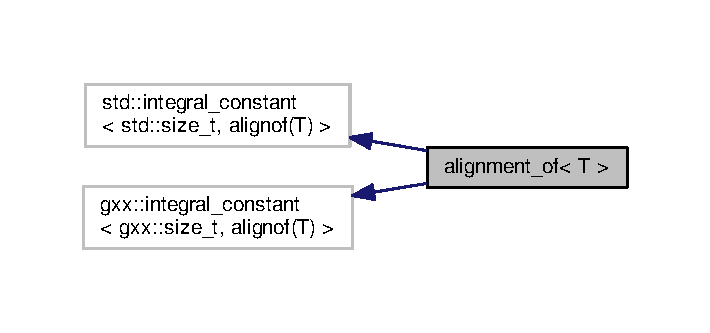
\includegraphics[width=341pt]{structalignment__of__inherit__graph}
\end{center}
\end{figure}


Collaboration diagram for alignment\+\_\+of$<$ T $>$\+:
\nopagebreak
\begin{figure}[H]
\begin{center}
\leavevmode
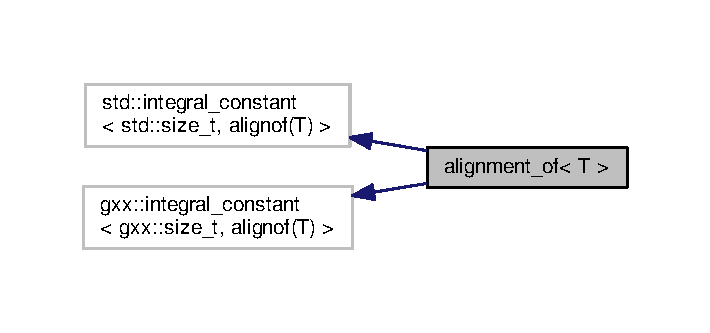
\includegraphics[width=341pt]{structalignment__of__coll__graph}
\end{center}
\end{figure}


The documentation for this struct was generated from the following file\+:\begin{DoxyCompactItemize}
\item 
/home/rfmeas/project/gxx/gxx/\+H\+I\+D\+E/utility/type\+\_\+relation.\+hpp\end{DoxyCompactItemize}

\hypertarget{classgxx_1_1AlignSpec}{}\section{gxx\+:\+:Align\+Spec Class Reference}
\label{classgxx_1_1AlignSpec}\index{gxx\+::\+Align\+Spec@{gxx\+::\+Align\+Spec}}


Inheritance diagram for gxx\+:\+:Align\+Spec\+:
% FIG 0


Collaboration diagram for gxx\+:\+:Align\+Spec\+:
% FIG 1
\subsection*{Public Member Functions}
\begin{DoxyCompactItemize}
\item 
Alignment {\bfseries align} () const \hypertarget{classgxx_1_1AlignSpec_a654c771a049d0e13db0b7f76ab4d1b3e}{}\label{classgxx_1_1AlignSpec_a654c771a049d0e13db0b7f76ab4d1b3e}

\item 
size\+\_\+t {\bfseries width} () const \hypertarget{classgxx_1_1AlignSpec_a04e46885c43f5723db9f5ea60167e2ed}{}\label{classgxx_1_1AlignSpec_a04e46885c43f5723db9f5ea60167e2ed}

\item 
char {\bfseries fill} () const \hypertarget{classgxx_1_1AlignSpec_a99f16ecd665cca2e55c81cf35e1ea25d}{}\label{classgxx_1_1AlignSpec_a99f16ecd665cca2e55c81cf35e1ea25d}

\item 
\hyperlink{classgxx_1_1AlignSpec}{Align\+Spec} \& {\bfseries align} (Alignment align)\hypertarget{classgxx_1_1AlignSpec_a1120c1314faf5dd458313fe5961b7c92}{}\label{classgxx_1_1AlignSpec_a1120c1314faf5dd458313fe5961b7c92}

\item 
\hyperlink{classgxx_1_1AlignSpec}{Align\+Spec} \& {\bfseries fill} (char fill)\hypertarget{classgxx_1_1AlignSpec_ad06cfdf3df3fb1a0cbcdfccd028f0b3d}{}\label{classgxx_1_1AlignSpec_ad06cfdf3df3fb1a0cbcdfccd028f0b3d}

\item 
\hyperlink{classgxx_1_1AlignSpec}{Align\+Spec} \& {\bfseries width} (size\+\_\+t width)\hypertarget{classgxx_1_1AlignSpec_a2092d47a38e4c52e5964a732e1ddfb52}{}\label{classgxx_1_1AlignSpec_a2092d47a38e4c52e5964a732e1ddfb52}

\end{DoxyCompactItemize}
\subsection*{Protected Attributes}
\begin{DoxyCompactItemize}
\item 
Alignment {\bfseries \+\_\+align} = Alignment\+::\+Default\hypertarget{classgxx_1_1AlignSpec_a0d77546b010f8017183deaf6d6ce5461}{}\label{classgxx_1_1AlignSpec_a0d77546b010f8017183deaf6d6ce5461}

\item 
char {\bfseries \+\_\+fill} = \textquotesingle{} \textquotesingle{}\hypertarget{classgxx_1_1AlignSpec_acf8cdffda2b9f09d89d064502ba5fb84}{}\label{classgxx_1_1AlignSpec_acf8cdffda2b9f09d89d064502ba5fb84}

\item 
size\+\_\+t {\bfseries \+\_\+width} = 0\hypertarget{classgxx_1_1AlignSpec_a139fcb8175b7bd492d6adcf64adccc1b}{}\label{classgxx_1_1AlignSpec_a139fcb8175b7bd492d6adcf64adccc1b}

\end{DoxyCompactItemize}


The documentation for this class was generated from the following file\+:\begin{DoxyCompactItemize}
\item 
/home/rfmeas/project/gxx/gxx/\+H\+I\+D\+E/io/text\+\_\+writer.\+h\end{DoxyCompactItemize}

\hypertarget{classgxx_1_1io_1_1AlignSpec}{}\section{gxx\+:\+:io\+:\+:Align\+Spec Class Reference}
\label{classgxx_1_1io_1_1AlignSpec}\index{gxx\+::io\+::\+Align\+Spec@{gxx\+::io\+::\+Align\+Spec}}


Inheritance diagram for gxx\+:\+:io\+:\+:Align\+Spec\+:
\nopagebreak
\begin{figure}[H]
\begin{center}
\leavevmode
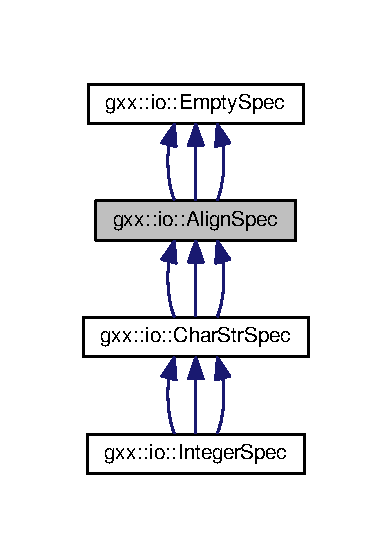
\includegraphics[width=188pt]{classgxx_1_1io_1_1AlignSpec__inherit__graph}
\end{center}
\end{figure}


Collaboration diagram for gxx\+:\+:io\+:\+:Align\+Spec\+:
\nopagebreak
\begin{figure}[H]
\begin{center}
\leavevmode
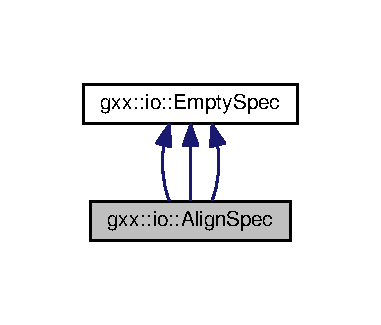
\includegraphics[width=183pt]{classgxx_1_1io_1_1AlignSpec__coll__graph}
\end{center}
\end{figure}
\subsection*{Public Member Functions}
\begin{DoxyCompactItemize}
\item 
Alignment {\bfseries align} () const \hypertarget{classgxx_1_1io_1_1AlignSpec_afa7b7b5e2307afc61fa158f33587cfa4}{}\label{classgxx_1_1io_1_1AlignSpec_afa7b7b5e2307afc61fa158f33587cfa4}

\item 
size\+\_\+t {\bfseries width} () const \hypertarget{classgxx_1_1io_1_1AlignSpec_a4025e3512a41207919ba0710aac5004e}{}\label{classgxx_1_1io_1_1AlignSpec_a4025e3512a41207919ba0710aac5004e}

\item 
char {\bfseries fill} () const \hypertarget{classgxx_1_1io_1_1AlignSpec_a055233b3c0e5558ba2bbfd1b6b2da858}{}\label{classgxx_1_1io_1_1AlignSpec_a055233b3c0e5558ba2bbfd1b6b2da858}

\item 
\hyperlink{classgxx_1_1io_1_1AlignSpec}{Align\+Spec} \& {\bfseries align} (Alignment align)\hypertarget{classgxx_1_1io_1_1AlignSpec_aaeae9560ec73fe1d3bcfbf556fc47e26}{}\label{classgxx_1_1io_1_1AlignSpec_aaeae9560ec73fe1d3bcfbf556fc47e26}

\item 
\hyperlink{classgxx_1_1io_1_1AlignSpec}{Align\+Spec} \& {\bfseries fill} (char fill)\hypertarget{classgxx_1_1io_1_1AlignSpec_a6f82e3aab453ce2ea5d93e37da6f3b01}{}\label{classgxx_1_1io_1_1AlignSpec_a6f82e3aab453ce2ea5d93e37da6f3b01}

\item 
\hyperlink{classgxx_1_1io_1_1AlignSpec}{Align\+Spec} \& {\bfseries width} (size\+\_\+t width)\hypertarget{classgxx_1_1io_1_1AlignSpec_a0cd7069f31fe0c417633f96c527b242b}{}\label{classgxx_1_1io_1_1AlignSpec_a0cd7069f31fe0c417633f96c527b242b}

\item 
Alignment {\bfseries align} () const \hypertarget{classgxx_1_1io_1_1AlignSpec_afa7b7b5e2307afc61fa158f33587cfa4}{}\label{classgxx_1_1io_1_1AlignSpec_afa7b7b5e2307afc61fa158f33587cfa4}

\item 
size\+\_\+t {\bfseries width} () const \hypertarget{classgxx_1_1io_1_1AlignSpec_a4025e3512a41207919ba0710aac5004e}{}\label{classgxx_1_1io_1_1AlignSpec_a4025e3512a41207919ba0710aac5004e}

\item 
char {\bfseries fill} () const \hypertarget{classgxx_1_1io_1_1AlignSpec_a055233b3c0e5558ba2bbfd1b6b2da858}{}\label{classgxx_1_1io_1_1AlignSpec_a055233b3c0e5558ba2bbfd1b6b2da858}

\item 
\hyperlink{classgxx_1_1io_1_1AlignSpec}{Align\+Spec} \& {\bfseries align} (Alignment align)\hypertarget{classgxx_1_1io_1_1AlignSpec_aaeae9560ec73fe1d3bcfbf556fc47e26}{}\label{classgxx_1_1io_1_1AlignSpec_aaeae9560ec73fe1d3bcfbf556fc47e26}

\item 
\hyperlink{classgxx_1_1io_1_1AlignSpec}{Align\+Spec} \& {\bfseries fill} (char fill)\hypertarget{classgxx_1_1io_1_1AlignSpec_a6f82e3aab453ce2ea5d93e37da6f3b01}{}\label{classgxx_1_1io_1_1AlignSpec_a6f82e3aab453ce2ea5d93e37da6f3b01}

\item 
\hyperlink{classgxx_1_1io_1_1AlignSpec}{Align\+Spec} \& {\bfseries width} (size\+\_\+t width)\hypertarget{classgxx_1_1io_1_1AlignSpec_a0cd7069f31fe0c417633f96c527b242b}{}\label{classgxx_1_1io_1_1AlignSpec_a0cd7069f31fe0c417633f96c527b242b}

\item 
Alignment {\bfseries align} () const \hypertarget{classgxx_1_1io_1_1AlignSpec_afa7b7b5e2307afc61fa158f33587cfa4}{}\label{classgxx_1_1io_1_1AlignSpec_afa7b7b5e2307afc61fa158f33587cfa4}

\item 
size\+\_\+t {\bfseries width} () const \hypertarget{classgxx_1_1io_1_1AlignSpec_a4025e3512a41207919ba0710aac5004e}{}\label{classgxx_1_1io_1_1AlignSpec_a4025e3512a41207919ba0710aac5004e}

\item 
char {\bfseries fill} () const \hypertarget{classgxx_1_1io_1_1AlignSpec_a055233b3c0e5558ba2bbfd1b6b2da858}{}\label{classgxx_1_1io_1_1AlignSpec_a055233b3c0e5558ba2bbfd1b6b2da858}

\item 
\hyperlink{classgxx_1_1io_1_1AlignSpec}{Align\+Spec} \& {\bfseries align} (Alignment align)\hypertarget{classgxx_1_1io_1_1AlignSpec_aaeae9560ec73fe1d3bcfbf556fc47e26}{}\label{classgxx_1_1io_1_1AlignSpec_aaeae9560ec73fe1d3bcfbf556fc47e26}

\item 
\hyperlink{classgxx_1_1io_1_1AlignSpec}{Align\+Spec} \& {\bfseries fill} (char fill)\hypertarget{classgxx_1_1io_1_1AlignSpec_a6f82e3aab453ce2ea5d93e37da6f3b01}{}\label{classgxx_1_1io_1_1AlignSpec_a6f82e3aab453ce2ea5d93e37da6f3b01}

\item 
\hyperlink{classgxx_1_1io_1_1AlignSpec}{Align\+Spec} \& {\bfseries width} (size\+\_\+t width)\hypertarget{classgxx_1_1io_1_1AlignSpec_a0cd7069f31fe0c417633f96c527b242b}{}\label{classgxx_1_1io_1_1AlignSpec_a0cd7069f31fe0c417633f96c527b242b}

\end{DoxyCompactItemize}
\subsection*{Protected Attributes}
\begin{DoxyCompactItemize}
\item 
Alignment {\bfseries \+\_\+align} = Alignment\+::\+Default\hypertarget{classgxx_1_1io_1_1AlignSpec_a2e9dd2412a1313263756ae2e8c6a839b}{}\label{classgxx_1_1io_1_1AlignSpec_a2e9dd2412a1313263756ae2e8c6a839b}

\item 
char {\bfseries \+\_\+fill} = \textquotesingle{} \textquotesingle{}\hypertarget{classgxx_1_1io_1_1AlignSpec_a534478199c8d086a8dffc381d98c075a}{}\label{classgxx_1_1io_1_1AlignSpec_a534478199c8d086a8dffc381d98c075a}

\item 
size\+\_\+t {\bfseries \+\_\+width} = 0\hypertarget{classgxx_1_1io_1_1AlignSpec_ab1ccba3dd4de2efcfa7e21a9f0a2a894}{}\label{classgxx_1_1io_1_1AlignSpec_ab1ccba3dd4de2efcfa7e21a9f0a2a894}

\end{DoxyCompactItemize}


The documentation for this class was generated from the following file\+:\begin{DoxyCompactItemize}
\item 
/home/rfmeas/project/gxx/gxx/\+H\+I\+D\+E/ionew/format\+\_\+writer.\+h\end{DoxyCompactItemize}

\hypertarget{classgxx_1_1allocator}{}\section{gxx\+:\+:allocator$<$ T $>$ Class Template Reference}
\label{classgxx_1_1allocator}\index{gxx\+::allocator$<$ T $>$@{gxx\+::allocator$<$ T $>$}}
\subsection*{Public Member Functions}
\begin{DoxyCompactItemize}
\item 
T $\ast$ {\bfseries allocate} (size\+\_\+t sz)\hypertarget{classgxx_1_1allocator_aa7136afcf5b11a1076ab924c01b5558e}{}\label{classgxx_1_1allocator_aa7136afcf5b11a1076ab924c01b5558e}

\item 
T $\ast$ {\bfseries reallocate} (void $\ast$ptr, size\+\_\+t sz)\hypertarget{classgxx_1_1allocator_a66dda3a13ad38faa584a69ce7a5c110d}{}\label{classgxx_1_1allocator_a66dda3a13ad38faa584a69ce7a5c110d}

\item 
void {\bfseries deallocate} (void $\ast$ptr)\hypertarget{classgxx_1_1allocator_a04b60ba5f185526c143770c3a93f322d}{}\label{classgxx_1_1allocator_a04b60ba5f185526c143770c3a93f322d}

\end{DoxyCompactItemize}


The documentation for this class was generated from the following file\+:\begin{DoxyCompactItemize}
\item 
/home/rfmeas/project/gxx/gxx/\+H\+I\+D\+E/allocator.\+h\end{DoxyCompactItemize}

\hypertarget{classgxx_1_1memory_1_1heap_1_1allocator}{}\section{gxx\+:\+:memory\+:\+:heap\+:\+:allocator$<$ T $>$ Class Template Reference}
\label{classgxx_1_1memory_1_1heap_1_1allocator}\index{gxx\+::memory\+::heap\+::allocator$<$ T $>$@{gxx\+::memory\+::heap\+::allocator$<$ T $>$}}
\subsection*{Public Types}
\begin{DoxyCompactItemize}
\item 
using {\bfseries value\+\_\+type} = T\hypertarget{classgxx_1_1memory_1_1heap_1_1allocator_a3c437d3eddd7c9f19655044c9bb41eb3}{}\label{classgxx_1_1memory_1_1heap_1_1allocator_a3c437d3eddd7c9f19655044c9bb41eb3}

\item 
using {\bfseries size\+\_\+type} = size\+\_\+t\hypertarget{classgxx_1_1memory_1_1heap_1_1allocator_a62af5de9efe92cc0782ca100e7bb1b80}{}\label{classgxx_1_1memory_1_1heap_1_1allocator_a62af5de9efe92cc0782ca100e7bb1b80}

\end{DoxyCompactItemize}
\subsection*{Public Member Functions}
\begin{DoxyCompactItemize}
\item 
{\bfseries allocator} (\hyperlink{classgxx_1_1memory_1_1heap}{heap} \&href)\hypertarget{classgxx_1_1memory_1_1heap_1_1allocator_a0477bfa3696987d7723ee2497d91a19d}{}\label{classgxx_1_1memory_1_1heap_1_1allocator_a0477bfa3696987d7723ee2497d91a19d}

\item 
T $\ast$ {\bfseries allocate} (size\+\_\+t n)\hypertarget{classgxx_1_1memory_1_1heap_1_1allocator_a1c2358d98178b5a2da0867d8290ea60b}{}\label{classgxx_1_1memory_1_1heap_1_1allocator_a1c2358d98178b5a2da0867d8290ea60b}

\item 
void {\bfseries deallocate} (T $\ast$ptr)\hypertarget{classgxx_1_1memory_1_1heap_1_1allocator_a0972ffae5174701244727be2ac5af8ce}{}\label{classgxx_1_1memory_1_1heap_1_1allocator_a0972ffae5174701244727be2ac5af8ce}

\item 
void {\bfseries deallocate} (T $\ast$ptr, size\+\_\+t n)\hypertarget{classgxx_1_1memory_1_1heap_1_1allocator_a0bea700f70c671ae4d1526a3e3d2cdaf}{}\label{classgxx_1_1memory_1_1heap_1_1allocator_a0bea700f70c671ae4d1526a3e3d2cdaf}

\end{DoxyCompactItemize}


The documentation for this class was generated from the following file\+:\begin{DoxyCompactItemize}
\item 
/home/rfmeas/project/gxx/gxx/memory/heap.\+h\end{DoxyCompactItemize}

\hypertarget{structgxx_1_1sgeom2_1_1arc}{}\section{gxx\+:\+:sgeom2\+:\+:arc$<$ T $>$ Struct Template Reference}
\label{structgxx_1_1sgeom2_1_1arc}\index{gxx\+::sgeom2\+::arc$<$ T $>$@{gxx\+::sgeom2\+::arc$<$ T $>$}}


Collaboration diagram for gxx\+:\+:sgeom2\+:\+:arc$<$ T $>$\+:
% FIG 0
\subsection*{Public Member Functions}
\begin{DoxyCompactItemize}
\item 
{\bfseries arc} (T x, T y, T w, T h, T a1, T a2)\hypertarget{structgxx_1_1sgeom2_1_1arc_afe3a2e6dc498bd2bd370d54d83c89e8c}{}\label{structgxx_1_1sgeom2_1_1arc_afe3a2e6dc498bd2bd370d54d83c89e8c}

\end{DoxyCompactItemize}
\subsection*{Public Attributes}
\begin{DoxyCompactItemize}
\item 
T {\bfseries x}\hypertarget{structgxx_1_1sgeom2_1_1arc_aceca8018c818f262614da61087acfaa5}{}\label{structgxx_1_1sgeom2_1_1arc_aceca8018c818f262614da61087acfaa5}

\item 
T {\bfseries y}\hypertarget{structgxx_1_1sgeom2_1_1arc_a21bb7ecae1eb51e584f949796b520bae}{}\label{structgxx_1_1sgeom2_1_1arc_a21bb7ecae1eb51e584f949796b520bae}

\item 
T {\bfseries w}\hypertarget{structgxx_1_1sgeom2_1_1arc_a6402054b1045e6bf4a8fe6c654a6d7ca}{}\label{structgxx_1_1sgeom2_1_1arc_a6402054b1045e6bf4a8fe6c654a6d7ca}

\item 
T {\bfseries h}\hypertarget{structgxx_1_1sgeom2_1_1arc_aba4128e7aeb022da0f5926c0a3054834}{}\label{structgxx_1_1sgeom2_1_1arc_aba4128e7aeb022da0f5926c0a3054834}

\item 
T {\bfseries a1}\hypertarget{structgxx_1_1sgeom2_1_1arc_a2808f13aba1886c257c990f43483082c}{}\label{structgxx_1_1sgeom2_1_1arc_a2808f13aba1886c257c990f43483082c}

\item 
T {\bfseries a2}\hypertarget{structgxx_1_1sgeom2_1_1arc_a6c965349a25cdc1585cc23efb41890d0}{}\label{structgxx_1_1sgeom2_1_1arc_a6c965349a25cdc1585cc23efb41890d0}

\end{DoxyCompactItemize}


The documentation for this struct was generated from the following file\+:\begin{DoxyCompactItemize}
\item 
/home/rfmeas/project/gxx/gxx/geom/sgeom2.\+h\end{DoxyCompactItemize}

\hypertarget{classgxx_1_1arglist}{}\section{gxx\+:\+:arglist Class Reference}
\label{classgxx_1_1arglist}\index{gxx\+::arglist@{gxx\+::arglist}}


Collaboration diagram for gxx\+:\+:arglist\+:
% FIG 0
\subsection*{Public Member Functions}
\begin{DoxyCompactItemize}
\item 
{\footnotesize template$<$typename... U\+Args$>$ }\\{\bfseries arglist} (U\+Args \&\&...args)\hypertarget{classgxx_1_1arglist_aec50946505f2a8258dff24e8ecb5ea50}{}\label{classgxx_1_1arglist_aec50946505f2a8258dff24e8ecb5ea50}

\item 
const \hyperlink{structgxx_1_1argument}{argument} \& {\bfseries operator\mbox{[}$\,$\mbox{]}} (int i) const \hypertarget{classgxx_1_1arglist_a6d5a62f369976094f60133c6c36c1f1d}{}\label{classgxx_1_1arglist_a6d5a62f369976094f60133c6c36c1f1d}

\item 
\hyperlink{structgxx_1_1argument}{argument} $\ast$ {\bfseries begin} ()\hypertarget{classgxx_1_1arglist_abbde7d4924c0ec1dc88ee050a63c6c04}{}\label{classgxx_1_1arglist_abbde7d4924c0ec1dc88ee050a63c6c04}

\item 
\hyperlink{structgxx_1_1argument}{argument} $\ast$ {\bfseries end} ()\hypertarget{classgxx_1_1arglist_ac58fdac6e49f8436db52e161f65eb97a}{}\label{classgxx_1_1arglist_ac58fdac6e49f8436db52e161f65eb97a}

\item 
int {\bfseries find\+\_\+name} (const char $\ast$name, size\+\_\+t len) const \hypertarget{classgxx_1_1arglist_acbbf22df9ba8ee8e4fd461d0c7357700}{}\label{classgxx_1_1arglist_acbbf22df9ba8ee8e4fd461d0c7357700}

\end{DoxyCompactItemize}
\subsection*{Public Attributes}
\begin{DoxyCompactItemize}
\item 
\hyperlink{structgxx_1_1argument}{argument} {\bfseries list} \mbox{[}15\mbox{]}\hypertarget{classgxx_1_1arglist_abb42300bed2be83c7498299a602f38a6}{}\label{classgxx_1_1arglist_abb42300bed2be83c7498299a602f38a6}

\item 
size\+\_\+t {\bfseries listsz}\hypertarget{classgxx_1_1arglist_aa1d072acb37922a83edf8c2145b64c89}{}\label{classgxx_1_1arglist_aa1d072acb37922a83edf8c2145b64c89}

\end{DoxyCompactItemize}


The documentation for this class was generated from the following files\+:\begin{DoxyCompactItemize}
\item 
/home/rfmeas/project/gxx/gxx/\+H\+I\+D\+E/arglist.\+h\item 
/home/rfmeas/project/gxx/gxx/\+H\+I\+D\+E/arglist.\+cpp\end{DoxyCompactItemize}

\hypertarget{structgxx_1_1argname}{}\section{gxx\+:\+:argname Struct Reference}
\label{structgxx_1_1argname}\index{gxx\+::argname@{gxx\+::argname}}


Collaboration diagram for gxx\+:\+:argname\+:\nopagebreak
\begin{figure}[H]
\begin{center}
\leavevmode
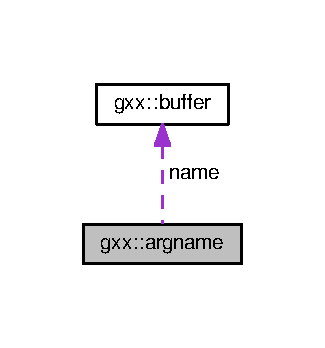
\includegraphics[width=156pt]{structgxx_1_1argname__coll__graph}
\end{center}
\end{figure}
\subsection*{Public Member Functions}
\begin{DoxyCompactItemize}
\item 
{\bfseries argname} (const \hyperlink{classgxx_1_1buffer}{gxx\+::buffer} \&\+\_\+name)\hypertarget{structgxx_1_1argname_af3d5cbd9a651c6c52d3020dc38359841}{}\label{structgxx_1_1argname_af3d5cbd9a651c6c52d3020dc38359841}

\item 
{\footnotesize template$<$typename T $>$ }\\constexpr \hyperlink{classgxx_1_1argpair}{argpair}$<$ typename std\+::remove\+\_\+reference$<$ T $>$\+::type $>$ {\bfseries operator=} (T \&\&body)\hypertarget{structgxx_1_1argname_a855215d4a37fc4aeb93f8870323f4269}{}\label{structgxx_1_1argname_a855215d4a37fc4aeb93f8870323f4269}

\item 
{\bfseries argname} (const char $\ast$\&name)\hypertarget{structgxx_1_1argname_a86bfc87d6776c03c70e63c5ffe9b927e}{}\label{structgxx_1_1argname_a86bfc87d6776c03c70e63c5ffe9b927e}

\item 
{\footnotesize template$<$typename T $>$ }\\constexpr \hyperlink{classgxx_1_1argpair}{argpair}$<$ T $>$ {\bfseries operator=} (T \&\&body)\hypertarget{structgxx_1_1argname_a8493b74166dcdb87fd967dc4687545e2}{}\label{structgxx_1_1argname_a8493b74166dcdb87fd967dc4687545e2}

\end{DoxyCompactItemize}
\subsection*{Public Attributes}
\begin{DoxyCompactItemize}
\item 
\hyperlink{classgxx_1_1buffer}{gxx\+::buffer} {\bfseries name}\hypertarget{structgxx_1_1argname_a61e6b9fabe2b3bbf028ae077d37d341a}{}\label{structgxx_1_1argname_a61e6b9fabe2b3bbf028ae077d37d341a}

\item 
const char $\ast$\& {\bfseries name}\hypertarget{structgxx_1_1argname_a36fff5dfb197d024e9ff3312dcb3afa4}{}\label{structgxx_1_1argname_a36fff5dfb197d024e9ff3312dcb3afa4}

\end{DoxyCompactItemize}


The documentation for this struct was generated from the following file\+:\begin{DoxyCompactItemize}
\item 
/home/rfmeas/project/gxx/gxx/arglist.\+h\end{DoxyCompactItemize}

\hypertarget{classgxx_1_1argpair}{}\section{gxx\+:\+:argpair$<$ T $>$ Struct Template Reference}
\label{classgxx_1_1argpair}\index{gxx\+::argpair$<$ T $>$@{gxx\+::argpair$<$ T $>$}}


Collaboration diagram for gxx\+:\+:argpair$<$ T $>$\+:
% FIG 0
\subsection*{Public Types}
\begin{DoxyCompactItemize}
\item 
using {\bfseries type} = T\hypertarget{classgxx_1_1argpair_a313a7427a6e4731dc2670f45aa41a5c0}{}\label{classgxx_1_1argpair_a313a7427a6e4731dc2670f45aa41a5c0}

\end{DoxyCompactItemize}
\subsection*{Public Member Functions}
\begin{DoxyCompactItemize}
\item 
constexpr {\bfseries argpair} (const \hyperlink{classgxx_1_1buffer}{gxx\+::buffer} \&\+\_\+name, void $\ast$\+\_\+body)\hypertarget{classgxx_1_1argpair_a0b82346ee3a5d25f0fd72b6be1e1cdd7}{}\label{classgxx_1_1argpair_a0b82346ee3a5d25f0fd72b6be1e1cdd7}

\item 
{\footnotesize template$<$typename U $>$ }\\constexpr {\bfseries argpair} (const char $\ast$name, U \&\&body)\hypertarget{classgxx_1_1argpair_aa8f02dc6696b89d6c26f8ac10eb965a8}{}\label{classgxx_1_1argpair_aa8f02dc6696b89d6c26f8ac10eb965a8}

\end{DoxyCompactItemize}
\subsection*{Public Attributes}
\begin{DoxyCompactItemize}
\item 
void $\ast$ {\bfseries body}\hypertarget{classgxx_1_1argpair_a7befa9a27d134c4c28ff8680b5337ef4}{}\label{classgxx_1_1argpair_a7befa9a27d134c4c28ff8680b5337ef4}

\item 
\hyperlink{classgxx_1_1buffer}{gxx\+::buffer} {\bfseries name}\hypertarget{classgxx_1_1argpair_a7d0492ac56c6b7e5d12af75a7508a48b}{}\label{classgxx_1_1argpair_a7d0492ac56c6b7e5d12af75a7508a48b}

\item 
T {\bfseries body}\hypertarget{classgxx_1_1argpair_ac1ac06472748b89a1af967b012e05aed}{}\label{classgxx_1_1argpair_ac1ac06472748b89a1af967b012e05aed}

\item 
const char $\ast$ {\bfseries name}\hypertarget{classgxx_1_1argpair_a2da2dc8aca332617ce4ae0638b177d9c}{}\label{classgxx_1_1argpair_a2da2dc8aca332617ce4ae0638b177d9c}

\end{DoxyCompactItemize}


The documentation for this struct was generated from the following file\+:\begin{DoxyCompactItemize}
\item 
/home/rfmeas/project/gxx/gxx/arglist.\+h\end{DoxyCompactItemize}

\hypertarget{structArgs}{}\section{Args$<$ T, Args $>$ Struct Template Reference}
\label{structArgs}\index{Args$<$ T, Args $>$@{Args$<$ T, Args $>$}}


Inheritance diagram for Args$<$ T, Args $>$\+:
% FIG 0


Collaboration diagram for Args$<$ T, Args $>$\+:
% FIG 1


The documentation for this struct was generated from the following file\+:\begin{DoxyCompactItemize}
\item 
/home/rfmeas/project/gxx/gxx/\+H\+I\+D\+E/utility/type\+\_\+traits.\+hpp\end{DoxyCompactItemize}

\hypertarget{structgxx_1_1argument}{}\section{gxx\+:\+:argument Struct Reference}
\label{structgxx_1_1argument}\index{gxx\+::argument@{gxx\+::argument}}
\subsection*{Public Member Functions}
\begin{DoxyCompactItemize}
\item 
{\bfseries argument} (void $\ast$ptr, void $\ast$func, const char $\ast$name=nullptr)\hypertarget{structgxx_1_1argument_a54267adb8fcd72e7bcc9acc46bb03444}{}\label{structgxx_1_1argument_a54267adb8fcd72e7bcc9acc46bb03444}

\end{DoxyCompactItemize}
\subsection*{Public Attributes}
\begin{DoxyCompactItemize}
\item 
void $\ast$ {\bfseries ptr}\hypertarget{structgxx_1_1argument_acb4b409905e981f89a3e1c74537994a1}{}\label{structgxx_1_1argument_acb4b409905e981f89a3e1c74537994a1}

\item 
void $\ast$ {\bfseries func}\hypertarget{structgxx_1_1argument_a76481d38590569300559e9d66b76dcac}{}\label{structgxx_1_1argument_a76481d38590569300559e9d66b76dcac}

\item 
const char $\ast$ {\bfseries name}\hypertarget{structgxx_1_1argument_a7ce8afbed3d14630bc0aae35bc3ac8f3}{}\label{structgxx_1_1argument_a7ce8afbed3d14630bc0aae35bc3ac8f3}

\end{DoxyCompactItemize}


The documentation for this struct was generated from the following file\+:\begin{DoxyCompactItemize}
\item 
/home/rfmeas/project/gxx/gxx/\+H\+I\+D\+E/arglist.\+h\end{DoxyCompactItemize}

\hypertarget{classgxx_1_1argument__temporary}{}\section{gxx\+:\+:argument\+\_\+temporary$<$ T, F $>$ Class Template Reference}
\label{classgxx_1_1argument__temporary}\index{gxx\+::argument\+\_\+temporary$<$ T, F $>$@{gxx\+::argument\+\_\+temporary$<$ T, F $>$}}


Collaboration diagram for gxx\+:\+:argument\+\_\+temporary$<$ T, F $>$\+:
\nopagebreak
\begin{figure}[H]
\begin{center}
\leavevmode
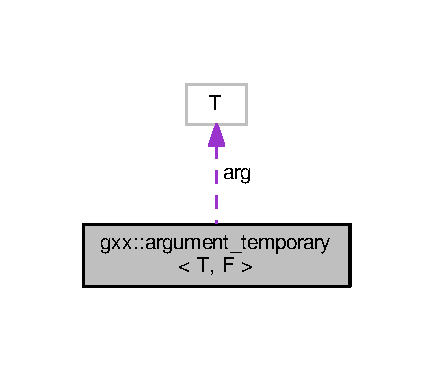
\includegraphics[width=208pt]{classgxx_1_1argument__temporary__coll__graph}
\end{center}
\end{figure}
\subsection*{Public Member Functions}
\begin{DoxyCompactItemize}
\item 
{\footnotesize template$<$typename U $>$ }\\{\bfseries argument\+\_\+temporary} (U \&\&arg, const char $\ast$name=nullptr)\hypertarget{classgxx_1_1argument__temporary_aac80deb9dda0d1a0201ed763154a7c91}{}\label{classgxx_1_1argument__temporary_aac80deb9dda0d1a0201ed763154a7c91}

\end{DoxyCompactItemize}
\subsection*{Public Attributes}
\begin{DoxyCompactItemize}
\item 
T {\bfseries arg}\hypertarget{classgxx_1_1argument__temporary_a529739c9d72fe83137a89257e8259bed}{}\label{classgxx_1_1argument__temporary_a529739c9d72fe83137a89257e8259bed}

\item 
const char $\ast$ {\bfseries name}\hypertarget{classgxx_1_1argument__temporary_a4ec886fb49488055c1a4a6c8aaf6e982}{}\label{classgxx_1_1argument__temporary_a4ec886fb49488055c1a4a6c8aaf6e982}

\end{DoxyCompactItemize}


The documentation for this class was generated from the following file\+:\begin{DoxyCompactItemize}
\item 
/home/rfmeas/project/gxx/gxx/\+H\+I\+D\+E/arglist.\+h\end{DoxyCompactItemize}

\hypertarget{classargvc__t}{}\section{argvc\+\_\+t Class Reference}
\label{classargvc__t}\index{argvc\+\_\+t@{argvc\+\_\+t}}


Inheritance diagram for argvc\+\_\+t\+:
\nopagebreak
\begin{figure}[H]
\begin{center}
\leavevmode
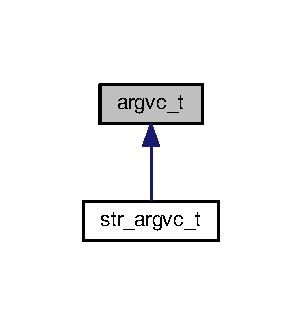
\includegraphics[width=145pt]{classargvc__t__inherit__graph}
\end{center}
\end{figure}
\subsection*{Public Member Functions}
\begin{DoxyCompactItemize}
\item 
void {\bfseries internal\+\_\+split} (char $\ast$str, char dv= \textquotesingle{} \textquotesingle{})\hypertarget{classargvc__t_abd61d46968ac80d6d58610340cdaa508}{}\label{classargvc__t_abd61d46968ac80d6d58610340cdaa508}

\item 
int {\bfseries argc} ()\hypertarget{classargvc__t_a769c05c3d5ef114497fec61afffeaa90}{}\label{classargvc__t_a769c05c3d5ef114497fec61afffeaa90}

\item 
char $\ast$$\ast$ {\bfseries argv} ()\hypertarget{classargvc__t_a5f9c39052a39f09702cb96f6932176fd}{}\label{classargvc__t_a5f9c39052a39f09702cb96f6932176fd}

\end{DoxyCompactItemize}


The documentation for this class was generated from the following file\+:\begin{DoxyCompactItemize}
\item 
/home/rfmeas/project/gxx/gxx/datastruct/argvc.\+h\end{DoxyCompactItemize}

\hypertarget{classgxx_1_1array__printable}{}\section{gxx\+:\+:array\+\_\+printable$<$ T $>$ Class Template Reference}
\label{classgxx_1_1array__printable}\index{gxx\+::array\+\_\+printable$<$ T $>$@{gxx\+::array\+\_\+printable$<$ T $>$}}
\subsection*{Public Member Functions}
\begin{DoxyCompactItemize}
\item 
size\+\_\+t {\bfseries print\+To} (\hyperlink{classgxx_1_1io_1_1ostream}{gxx\+::io\+::ostream} \&o) const \hypertarget{classgxx_1_1array__printable_a90cd593367e3f157ffbc2d077b942962}{}\label{classgxx_1_1array__printable_a90cd593367e3f157ffbc2d077b942962}

\end{DoxyCompactItemize}


The documentation for this class was generated from the following file\+:\begin{DoxyCompactItemize}
\item 
/home/rfmeas/project/gxx/gxx/print/printable.\+h\end{DoxyCompactItemize}

\hypertarget{classgxx_1_1gstuff_1_1automate}{}\section{gxx\+:\+:gstuff\+:\+:automate Class Reference}
\label{classgxx_1_1gstuff_1_1automate}\index{gxx\+::gstuff\+::automate@{gxx\+::gstuff\+::automate}}
\subsection*{Public Member Functions}
\begin{DoxyCompactItemize}
\item 
{\bfseries A\+C\+C\+E\+S\+S\+OR} (debug\+\_\+mode, \+\_\+debug)\hypertarget{classgxx_1_1gstuff_1_1automate_a36821652fd6f020cdf300cd2839a23da}{}\label{classgxx_1_1gstuff_1_1automate_a36821652fd6f020cdf300cd2839a23da}

\item 
{\bfseries automate} (\hyperlink{classgxx_1_1buffer}{gxx\+::buffer} buf)\hypertarget{classgxx_1_1gstuff_1_1automate_a615464ac28650b81d9cc08dcdaef1115}{}\label{classgxx_1_1gstuff_1_1automate_a615464ac28650b81d9cc08dcdaef1115}

\item 
void {\bfseries init} ()\hypertarget{classgxx_1_1gstuff_1_1automate_a254012d093a9f5d3c7ceb8a5e34bc68f}{}\label{classgxx_1_1gstuff_1_1automate_a254012d093a9f5d3c7ceb8a5e34bc68f}

\item 
void {\bfseries invoke\+\_\+callback} ()\hypertarget{classgxx_1_1gstuff_1_1automate_aa538f15878a88a4b99bc697a4013b029}{}\label{classgxx_1_1gstuff_1_1automate_aa538f15878a88a4b99bc697a4013b029}

\item 
void {\bfseries set\+\_\+callback} (\hyperlink{classgxx_1_1delegate}{gxx\+::delegate}$<$ void, \hyperlink{classgxx_1_1buffer}{gxx\+::buffer} $>$ dlg)\hypertarget{classgxx_1_1gstuff_1_1automate_a6bd819c94315fb909e707fd15d721201}{}\label{classgxx_1_1gstuff_1_1automate_a6bd819c94315fb909e707fd15d721201}

\item 
void {\bfseries setstate} (int n)\hypertarget{classgxx_1_1gstuff_1_1automate_a1c4d32b4b8011495d6c4545f79846c55}{}\label{classgxx_1_1gstuff_1_1automate_a1c4d32b4b8011495d6c4545f79846c55}

\item 
void {\bfseries newchar} (char c)\hypertarget{classgxx_1_1gstuff_1_1automate_af3859c6b82bca73030ad74d3d4ed360d}{}\label{classgxx_1_1gstuff_1_1automate_af3859c6b82bca73030ad74d3d4ed360d}

\end{DoxyCompactItemize}


The documentation for this class was generated from the following file\+:\begin{DoxyCompactItemize}
\item 
/home/rfmeas/project/gxx/gxx/gstuff/automate.\+h\end{DoxyCompactItemize}

\hypertarget{classgxx_1_1geom3_1_1axis}{}\section{gxx\+:\+:geom3\+:\+:axis Class Reference}
\label{classgxx_1_1geom3_1_1axis}\index{gxx\+::geom3\+::axis@{gxx\+::geom3\+::axis}}


Collaboration diagram for gxx\+:\+:geom3\+:\+:axis\+:
% FIG 0
\subsection*{Public Member Functions}
\begin{DoxyCompactItemize}
\item 
{\bfseries axis} (\hyperlink{classgxx_1_1geom3_1_1point}{point} l, \hyperlink{classgxx_1_1geom3_1_1direction}{direction} d)\hypertarget{classgxx_1_1geom3_1_1axis_a08fd792af64f78466f31809fbbc646a6}{}\label{classgxx_1_1geom3_1_1axis_a08fd792af64f78466f31809fbbc646a6}

\item 
{\bfseries C\+O\+N\+S\+T\+R\+E\+F\+\_\+\+G\+E\+T\+T\+ER} (loc, l)\hypertarget{classgxx_1_1geom3_1_1axis_adee32a748ca587261f8a7b7f74510b12}{}\label{classgxx_1_1geom3_1_1axis_adee32a748ca587261f8a7b7f74510b12}

\item 
{\bfseries C\+O\+N\+S\+T\+R\+E\+F\+\_\+\+G\+E\+T\+T\+ER} (dir, d)\hypertarget{classgxx_1_1geom3_1_1axis_a5a23fb24c936dbef75e07a92182f4df7}{}\label{classgxx_1_1geom3_1_1axis_a5a23fb24c936dbef75e07a92182f4df7}

\end{DoxyCompactItemize}
\subsection*{Public Attributes}
\begin{DoxyCompactItemize}
\item 
\hyperlink{classgxx_1_1geom3_1_1point}{point} {\bfseries l}\hypertarget{classgxx_1_1geom3_1_1axis_a346d41bf4307d5876fa230ee778973e7}{}\label{classgxx_1_1geom3_1_1axis_a346d41bf4307d5876fa230ee778973e7}

\item 
\hyperlink{classgxx_1_1geom3_1_1direction}{direction} {\bfseries d}\hypertarget{classgxx_1_1geom3_1_1axis_a096551f9e9c6dfff8366fc12ea4d6450}{}\label{classgxx_1_1geom3_1_1axis_a096551f9e9c6dfff8366fc12ea4d6450}

\end{DoxyCompactItemize}


The documentation for this class was generated from the following files\+:\begin{DoxyCompactItemize}
\item 
/home/rfmeas/project/gxx/gxx/geom/geom3.\+h\item 
/home/rfmeas/project/gxx/gxx/geom/\+H\+I\+D\+E/base.\+cpp\end{DoxyCompactItemize}

\hypertarget{classgxx_1_1geom3_1_1axis2}{}\section{gxx\+:\+:geom3\+:\+:axis2 Class Reference}
\label{classgxx_1_1geom3_1_1axis2}\index{gxx\+::geom3\+::axis2@{gxx\+::geom3\+::axis2}}


Collaboration diagram for gxx\+:\+:geom3\+:\+:axis2\+:
\nopagebreak
\begin{figure}[H]
\begin{center}
\leavevmode
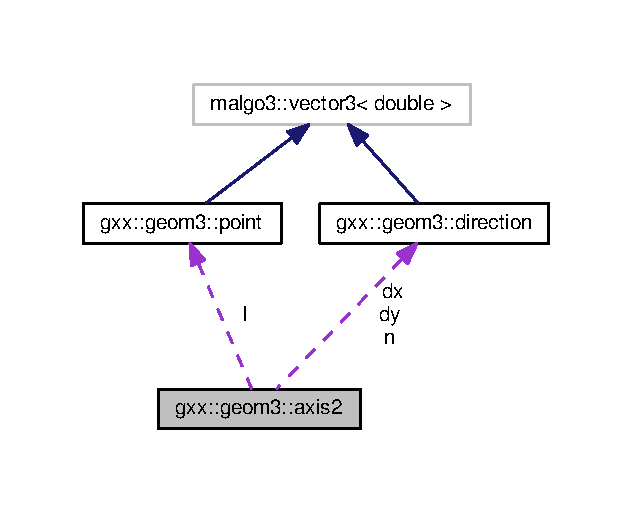
\includegraphics[width=304pt]{classgxx_1_1geom3_1_1axis2__coll__graph}
\end{center}
\end{figure}
\subsection*{Public Member Functions}
\begin{DoxyCompactItemize}
\item 
{\bfseries axis2} (\hyperlink{classgxx_1_1geom3_1_1point}{point} l, \hyperlink{classgxx_1_1geom3_1_1direction}{direction} n, \hyperlink{classgxx_1_1geom3_1_1direction}{direction} vx)\hypertarget{classgxx_1_1geom3_1_1axis2_a807a7398df31fbcba7fec71b2c89d8c8}{}\label{classgxx_1_1geom3_1_1axis2_a807a7398df31fbcba7fec71b2c89d8c8}

\item 
{\bfseries axis2} (\hyperlink{classgxx_1_1geom3_1_1point}{point} l, \hyperlink{classgxx_1_1geom3_1_1direction}{direction} n)\hypertarget{classgxx_1_1geom3_1_1axis2_a6e3462034e771e2719acc408e6df9ec0}{}\label{classgxx_1_1geom3_1_1axis2_a6e3462034e771e2719acc408e6df9ec0}

\item 
{\bfseries axis2} (\hyperlink{classgxx_1_1geom3_1_1point}{point} a, \hyperlink{classgxx_1_1geom3_1_1point}{point} b, \hyperlink{classgxx_1_1geom3_1_1point}{point} c)\hypertarget{classgxx_1_1geom3_1_1axis2_a3ee7933a05115475fd63bd4c829cbc81}{}\label{classgxx_1_1geom3_1_1axis2_a3ee7933a05115475fd63bd4c829cbc81}

\item 
\hyperlink{classmalgo_1_1vector2}{gxx\+::geom2\+::vector} {\bfseries project\+\_\+vector} (const malgo3\+::vector3$<$ double $>$ \&vec) const \hypertarget{classgxx_1_1geom3_1_1axis2_a7d2f121065e1677e603b2eb0da53124b}{}\label{classgxx_1_1geom3_1_1axis2_a7d2f121065e1677e603b2eb0da53124b}

\item 
\hyperlink{classmalgo_1_1vector2}{gxx\+::geom2\+::point} {\bfseries project\+\_\+point} (const malgo3\+::vector3$<$ double $>$ \&pnt) const \hypertarget{classgxx_1_1geom3_1_1axis2_a33e08456b3b043500219a016df956db7}{}\label{classgxx_1_1geom3_1_1axis2_a33e08456b3b043500219a016df956db7}

\item 
{\bfseries C\+O\+N\+S\+T\+R\+E\+F\+\_\+\+G\+E\+T\+T\+ER} (loc, l)\hypertarget{classgxx_1_1geom3_1_1axis2_ab06da104334da34a74703e3e1e4ac91d}{}\label{classgxx_1_1geom3_1_1axis2_ab06da104334da34a74703e3e1e4ac91d}

\item 
{\bfseries C\+O\+N\+S\+T\+R\+E\+F\+\_\+\+G\+E\+T\+T\+ER} (dirx, dx)\hypertarget{classgxx_1_1geom3_1_1axis2_ae6dda12eb6d1e7bb6443c688dad430f9}{}\label{classgxx_1_1geom3_1_1axis2_ae6dda12eb6d1e7bb6443c688dad430f9}

\item 
{\bfseries C\+O\+N\+S\+T\+R\+E\+F\+\_\+\+G\+E\+T\+T\+ER} (diry, dy)\hypertarget{classgxx_1_1geom3_1_1axis2_a8a39a8b8e3f47ab9f77804fecd070608}{}\label{classgxx_1_1geom3_1_1axis2_a8a39a8b8e3f47ab9f77804fecd070608}

\item 
size\+\_\+t {\bfseries print\+To} (\hyperlink{classgxx_1_1io_1_1ostream}{gxx\+::io\+::ostream} \&o) const \hypertarget{classgxx_1_1geom3_1_1axis2_a1a7d141a3bd974d93b0e34551aac43fd}{}\label{classgxx_1_1geom3_1_1axis2_a1a7d141a3bd974d93b0e34551aac43fd}

\end{DoxyCompactItemize}
\subsection*{Public Attributes}
\begin{DoxyCompactItemize}
\item 
\hyperlink{classgxx_1_1geom3_1_1point}{point} {\bfseries l}\hypertarget{classgxx_1_1geom3_1_1axis2_a8b647f744b39e87341c39ed50c7b04a8}{}\label{classgxx_1_1geom3_1_1axis2_a8b647f744b39e87341c39ed50c7b04a8}

\item 
\hyperlink{classgxx_1_1geom3_1_1direction}{direction} {\bfseries n}\hypertarget{classgxx_1_1geom3_1_1axis2_aad35f7babab12fe7ca80a1e9ff10ce25}{}\label{classgxx_1_1geom3_1_1axis2_aad35f7babab12fe7ca80a1e9ff10ce25}

\item 
\hyperlink{classgxx_1_1geom3_1_1direction}{direction} {\bfseries dx}\hypertarget{classgxx_1_1geom3_1_1axis2_a854199c278119e5f5ff3391bee1cd1cc}{}\label{classgxx_1_1geom3_1_1axis2_a854199c278119e5f5ff3391bee1cd1cc}

\item 
\hyperlink{classgxx_1_1geom3_1_1direction}{direction} {\bfseries dy}\hypertarget{classgxx_1_1geom3_1_1axis2_a9a3f95b98ae9aba91bb3cd50b9668a27}{}\label{classgxx_1_1geom3_1_1axis2_a9a3f95b98ae9aba91bb3cd50b9668a27}

\end{DoxyCompactItemize}


The documentation for this class was generated from the following file\+:\begin{DoxyCompactItemize}
\item 
/home/rfmeas/project/gxx/gxx/geom/geom3.\+h\end{DoxyCompactItemize}

\hypertarget{classgxx_1_1geom3_1_1axis3}{}\section{gxx\+:\+:geom3\+:\+:axis3 Class Reference}
\label{classgxx_1_1geom3_1_1axis3}\index{gxx\+::geom3\+::axis3@{gxx\+::geom3\+::axis3}}


Collaboration diagram for gxx\+:\+:geom3\+:\+:axis3\+:
% FIG 0
\subsection*{Public Member Functions}
\begin{DoxyCompactItemize}
\item 
{\bfseries axis3} (\hyperlink{classgxx_1_1geom3_1_1point}{point} l, \hyperlink{classgxx_1_1geom3_1_1direction}{direction} n, \hyperlink{classgxx_1_1geom3_1_1direction}{direction} vx)\hypertarget{classgxx_1_1geom3_1_1axis3_ad60e27afc66929ac5579565719af4be3}{}\label{classgxx_1_1geom3_1_1axis3_ad60e27afc66929ac5579565719af4be3}

\item 
{\bfseries C\+O\+N\+S\+T\+R\+E\+F\+\_\+\+G\+E\+T\+T\+ER} (loc, l)\hypertarget{classgxx_1_1geom3_1_1axis3_ac4a6a1138d9fbb0b5400d953e2de1e4f}{}\label{classgxx_1_1geom3_1_1axis3_ac4a6a1138d9fbb0b5400d953e2de1e4f}

\item 
{\bfseries C\+O\+N\+S\+T\+R\+E\+F\+\_\+\+G\+E\+T\+T\+ER} (dirx, dx)\hypertarget{classgxx_1_1geom3_1_1axis3_a84d77864f3562a9bd409bb4ccb6dc267}{}\label{classgxx_1_1geom3_1_1axis3_a84d77864f3562a9bd409bb4ccb6dc267}

\item 
{\bfseries C\+O\+N\+S\+T\+R\+E\+F\+\_\+\+G\+E\+T\+T\+ER} (diry, dy)\hypertarget{classgxx_1_1geom3_1_1axis3_a1fc769c2c97f01447730bbc2e605239c}{}\label{classgxx_1_1geom3_1_1axis3_a1fc769c2c97f01447730bbc2e605239c}

\item 
{\bfseries C\+O\+N\+S\+T\+R\+E\+F\+\_\+\+G\+E\+T\+T\+ER} (dirz, dz)\hypertarget{classgxx_1_1geom3_1_1axis3_af3bfe0d05e7d33a2c282f5615c76481d}{}\label{classgxx_1_1geom3_1_1axis3_af3bfe0d05e7d33a2c282f5615c76481d}

\item 
size\+\_\+t {\bfseries print\+To} (\hyperlink{classgxx_1_1io_1_1ostream}{gxx\+::io\+::ostream} \&o) const \hypertarget{classgxx_1_1geom3_1_1axis3_af9d74faa5dc4bd0db905acd70f4c3a8b}{}\label{classgxx_1_1geom3_1_1axis3_af9d74faa5dc4bd0db905acd70f4c3a8b}

\end{DoxyCompactItemize}
\subsection*{Public Attributes}
\begin{DoxyCompactItemize}
\item 
\hyperlink{classgxx_1_1geom3_1_1point}{point} {\bfseries l}\hypertarget{classgxx_1_1geom3_1_1axis3_acaf815f5b992130f930e6e153b5c5839}{}\label{classgxx_1_1geom3_1_1axis3_acaf815f5b992130f930e6e153b5c5839}

\item 
\hyperlink{classgxx_1_1geom3_1_1direction}{direction} {\bfseries dx}\hypertarget{classgxx_1_1geom3_1_1axis3_a93d1340ebbf0c155bc6b8eb0ecfdaab4}{}\label{classgxx_1_1geom3_1_1axis3_a93d1340ebbf0c155bc6b8eb0ecfdaab4}

\item 
\hyperlink{classgxx_1_1geom3_1_1direction}{direction} {\bfseries dy}\hypertarget{classgxx_1_1geom3_1_1axis3_abd942ab6e426e41dcae1edb8ce790d3f}{}\label{classgxx_1_1geom3_1_1axis3_abd942ab6e426e41dcae1edb8ce790d3f}

\item 
\hyperlink{classgxx_1_1geom3_1_1direction}{direction} {\bfseries dz}\hypertarget{classgxx_1_1geom3_1_1axis3_adc94694684edd334578748efb4b44068}{}\label{classgxx_1_1geom3_1_1axis3_adc94694684edd334578748efb4b44068}

\end{DoxyCompactItemize}


The documentation for this class was generated from the following file\+:\begin{DoxyCompactItemize}
\item 
/home/rfmeas/project/gxx/gxx/geom/geom3.\+h\end{DoxyCompactItemize}

\hypertarget{classgxx_1_1axis__correction__table}{}\section{gxx\+:\+:axis\+\_\+correction\+\_\+table Class Reference}
\label{classgxx_1_1axis__correction__table}\index{gxx\+::axis\+\_\+correction\+\_\+table@{gxx\+::axis\+\_\+correction\+\_\+table}}


The documentation for this class was generated from the following file\+:\begin{DoxyCompactItemize}
\item 
/home/rfmeas/project/gxx/gxx/geom/\+H\+I\+D\+E/coordcorrection.\+h\end{DoxyCompactItemize}

\hypertarget{structgxx_1_1rpc_1_1basic__invoker}{}\section{gxx\+:\+:rpc\+:\+:basic\+\_\+invoker$<$ Input, Output $>$ Struct Template Reference}
\label{structgxx_1_1rpc_1_1basic__invoker}\index{gxx\+::rpc\+::basic\+\_\+invoker$<$ Input, Output $>$@{gxx\+::rpc\+::basic\+\_\+invoker$<$ Input, Output $>$}}


Inheritance diagram for gxx\+:\+:rpc\+:\+:basic\+\_\+invoker$<$ Input, Output $>$\+:
% FIG 0
\subsection*{Public Member Functions}
\begin{DoxyCompactItemize}
\item 
virtual status {\bfseries invoke} (Input \&, Output \&)=0\hypertarget{structgxx_1_1rpc_1_1basic__invoker_a2e5f0f0570a895e7c367384a6ccd67e3}{}\label{structgxx_1_1rpc_1_1basic__invoker_a2e5f0f0570a895e7c367384a6ccd67e3}

\end{DoxyCompactItemize}


The documentation for this struct was generated from the following file\+:\begin{DoxyCompactItemize}
\item 
/home/rfmeas/project/gxx/gxx/rpc/invoker.\+h\end{DoxyCompactItemize}

\hypertarget{classgxx_1_1basic__slot}{}\section{gxx\+:\+:basic\+\_\+slot$<$ Args $>$ Class Template Reference}
\label{classgxx_1_1basic__slot}\index{gxx\+::basic\+\_\+slot$<$ Args $>$@{gxx\+::basic\+\_\+slot$<$ Args $>$}}


Collaboration diagram for gxx\+:\+:basic\+\_\+slot$<$ Args $>$\+:
\nopagebreak
\begin{figure}[H]
\begin{center}
\leavevmode
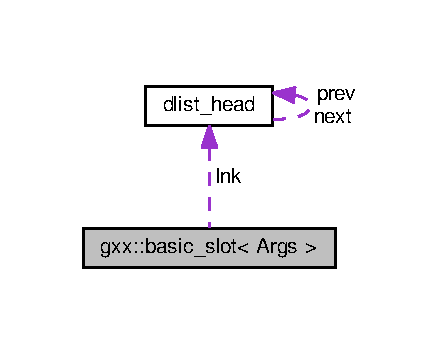
\includegraphics[width=211pt]{classgxx_1_1basic__slot__coll__graph}
\end{center}
\end{figure}
\subsection*{Public Member Functions}
\begin{DoxyCompactItemize}
\item 
virtual void {\bfseries invoke} (Args...\+args)=0\hypertarget{classgxx_1_1basic__slot_acd9dd2218eceeede793b07f6f5a104a7}{}\label{classgxx_1_1basic__slot_acd9dd2218eceeede793b07f6f5a104a7}

\item 
void {\bfseries unconnect\+\_\+on\+\_\+invoke} (bool en)\hypertarget{classgxx_1_1basic__slot_ae6b3166a79c01e9b818b84e2cd99a823}{}\label{classgxx_1_1basic__slot_ae6b3166a79c01e9b818b84e2cd99a823}

\end{DoxyCompactItemize}
\subsection*{Public Attributes}
\begin{DoxyCompactItemize}
\item 
\hyperlink{structdlist__head}{dlist\+\_\+head} {\bfseries lnk}\hypertarget{classgxx_1_1basic__slot_ac6efa5e7b653f960e7c9a492a819d277}{}\label{classgxx_1_1basic__slot_ac6efa5e7b653f960e7c9a492a819d277}

\item 
uint8\+\_\+t {\bfseries flag\+\_\+unconnect\+\_\+on\+\_\+invoke}\+: 1\hypertarget{classgxx_1_1basic__slot_a535fb110c1ba08716c49a84909008f5e}{}\label{classgxx_1_1basic__slot_a535fb110c1ba08716c49a84909008f5e}

\end{DoxyCompactItemize}
\subsection*{Protected Attributes}
\begin{DoxyCompactItemize}
\item 
\begin{tabbing}
xx\=xx\=xx\=xx\=xx\=xx\=xx\=xx\=xx\=\kill
struct \{\\
\>uint8\_t {\bfseries flag\_unconnect\_on\_invoke}: 1\\
\}; \hypertarget{classgxx_1_1basic__slot_a9e4d31168626180fea20e5e1fffb4ecc}{}\label{classgxx_1_1basic__slot_a9e4d31168626180fea20e5e1fffb4ecc}
\\

\end{tabbing}\end{DoxyCompactItemize}


The documentation for this class was generated from the following file\+:\begin{DoxyCompactItemize}
\item 
/home/rfmeas/project/gxx/gxx/event/\+H\+I\+D\+E/slot.\+h\end{DoxyCompactItemize}

\hypertarget{classgxx_1_1basic__string}{}\section{gxx\+:\+:basic\+\_\+string$<$ Allocator $>$ Class Template Reference}
\label{classgxx_1_1basic__string}\index{gxx\+::basic\+\_\+string$<$ Allocator $>$@{gxx\+::basic\+\_\+string$<$ Allocator $>$}}
\subsection*{Public Member Functions}
\begin{DoxyCompactItemize}
\item 
{\bfseries C\+O\+N\+S\+T\+R\+E\+F\+\_\+\+G\+E\+T\+T\+ER} (data, m\+\_\+data)\hypertarget{classgxx_1_1basic__string_a25a7518772b232e74b483d4e1667f689}{}\label{classgxx_1_1basic__string_a25a7518772b232e74b483d4e1667f689}

\item 
{\bfseries C\+O\+N\+S\+T\+R\+E\+F\+\_\+\+G\+E\+T\+T\+ER} (capacity, m\+\_\+capacity)\hypertarget{classgxx_1_1basic__string_a5e2120a19527fe9e506415f72faf3b61}{}\label{classgxx_1_1basic__string_a5e2120a19527fe9e506415f72faf3b61}

\item 
{\bfseries C\+O\+N\+S\+T\+R\+E\+F\+\_\+\+G\+E\+T\+T\+ER} (size, m\+\_\+size)\hypertarget{classgxx_1_1basic__string_a50d12d0faae89c00ed26cc51508b6a2b}{}\label{classgxx_1_1basic__string_a50d12d0faae89c00ed26cc51508b6a2b}

\item 
{\bfseries basic\+\_\+string} (const \hyperlink{classgxx_1_1basic__string}{basic\+\_\+string} \&other)\hypertarget{classgxx_1_1basic__string_a7995ab02a7a368afa030f863f2894c84}{}\label{classgxx_1_1basic__string_a7995ab02a7a368afa030f863f2894c84}

\item 
{\bfseries basic\+\_\+string} (\hyperlink{classgxx_1_1basic__string}{basic\+\_\+string} \&\&other)\hypertarget{classgxx_1_1basic__string_a6e1ecf6134e1e98107321c6b25a70aa3}{}\label{classgxx_1_1basic__string_a6e1ecf6134e1e98107321c6b25a70aa3}

\item 
{\bfseries basic\+\_\+string} (const char $\ast$str)\hypertarget{classgxx_1_1basic__string_a0632c1a00f88abd0326b0248537338aa}{}\label{classgxx_1_1basic__string_a0632c1a00f88abd0326b0248537338aa}

\item 
{\bfseries basic\+\_\+string} (const char $\ast$str, size\+\_\+t sz)\hypertarget{classgxx_1_1basic__string_a85e176434218cd67ebc6686ddfc4f5c2}{}\label{classgxx_1_1basic__string_a85e176434218cd67ebc6686ddfc4f5c2}

\item 
\hyperlink{classgxx_1_1basic__string}{basic\+\_\+string} \& {\bfseries copy} (const char $\ast$cstr, size\+\_\+t length)\hypertarget{classgxx_1_1basic__string_ac8b82ed2e52861d91f85251513cb0793}{}\label{classgxx_1_1basic__string_ac8b82ed2e52861d91f85251513cb0793}

\item 
void {\bfseries move} (\hyperlink{classgxx_1_1basic__string}{basic\+\_\+string} \&rhs)\hypertarget{classgxx_1_1basic__string_a4b59fd59bc93889b0e883a8c46d74b2a}{}\label{classgxx_1_1basic__string_a4b59fd59bc93889b0e883a8c46d74b2a}

\item 
void {\bfseries invalidate} (void)\hypertarget{classgxx_1_1basic__string_a389fd4c801d67aa8a43c644d855cd1ba}{}\label{classgxx_1_1basic__string_a389fd4c801d67aa8a43c644d855cd1ba}

\item 
\hyperlink{classgxx_1_1basic__string}{basic\+\_\+string} \& {\bfseries operator=} (const \hyperlink{classgxx_1_1basic__string}{basic\+\_\+string} \&rhs)\hypertarget{classgxx_1_1basic__string_a4df36570d4a8de7d36f5f2b9c9bad840}{}\label{classgxx_1_1basic__string_a4df36570d4a8de7d36f5f2b9c9bad840}

\item 
\hyperlink{classgxx_1_1basic__string}{basic\+\_\+string} \& {\bfseries operator=} (\hyperlink{classgxx_1_1basic__string}{basic\+\_\+string} \&\&rval)\hypertarget{classgxx_1_1basic__string_a0d1d5ff080536bfc807a9921d25d3717}{}\label{classgxx_1_1basic__string_a0d1d5ff080536bfc807a9921d25d3717}

\item 
\hyperlink{classgxx_1_1basic__string}{basic\+\_\+string} \& {\bfseries operator=} (const char $\ast$str)\hypertarget{classgxx_1_1basic__string_a410f48c9f9907d8195007fc01388dd1a}{}\label{classgxx_1_1basic__string_a410f48c9f9907d8195007fc01388dd1a}

\item 
const char $\ast$ {\bfseries c\+\_\+str} ()\hypertarget{classgxx_1_1basic__string_a2410cc6b56b44ac06d7bcfa6e33c4afd}{}\label{classgxx_1_1basic__string_a2410cc6b56b44ac06d7bcfa6e33c4afd}

\item 
char $\ast$ {\bfseries begin} ()\hypertarget{classgxx_1_1basic__string_a19e4a5799d86b98308bfb12a146b8de5}{}\label{classgxx_1_1basic__string_a19e4a5799d86b98308bfb12a146b8de5}

\item 
char $\ast$ {\bfseries end} ()\hypertarget{classgxx_1_1basic__string_af92b9ebe9e0b441e6c7d31c19357692f}{}\label{classgxx_1_1basic__string_af92b9ebe9e0b441e6c7d31c19357692f}

\item 
unsigned char {\bfseries reserve} (size\+\_\+t sz)\hypertarget{classgxx_1_1basic__string_aa28d8acfdef6cdc7219c99e263de1d6f}{}\label{classgxx_1_1basic__string_aa28d8acfdef6cdc7219c99e263de1d6f}

\item 
unsigned char {\bfseries change\+Buffer} (size\+\_\+t max\+Str\+Len)\hypertarget{classgxx_1_1basic__string_ab1b9c34bd19917bd75bc4588375e0b5d}{}\label{classgxx_1_1basic__string_ab1b9c34bd19917bd75bc4588375e0b5d}

\item 
unsigned char {\bfseries concat} (const char $\ast$cstr, size\+\_\+t length)\hypertarget{classgxx_1_1basic__string_af9d3474e6020296ff5834b9cc020886c}{}\label{classgxx_1_1basic__string_af9d3474e6020296ff5834b9cc020886c}

\item 
unsigned char {\bfseries concat} (char c)\hypertarget{classgxx_1_1basic__string_a66da792a10430b3187b8b2ba59d3503a}{}\label{classgxx_1_1basic__string_a66da792a10430b3187b8b2ba59d3503a}

\item 
unsigned char {\bfseries concat} (const char $\ast$cstr)\hypertarget{classgxx_1_1basic__string_aeeba3c5dde2f85ca2598ecd5ff83f7f6}{}\label{classgxx_1_1basic__string_aeeba3c5dde2f85ca2598ecd5ff83f7f6}

\item 
unsigned char {\bfseries concat} (int8\+\_\+t num, uint8\+\_\+t base)\hypertarget{classgxx_1_1basic__string_ab89ef969b937e9f566a08115b21943fe}{}\label{classgxx_1_1basic__string_ab89ef969b937e9f566a08115b21943fe}

\item 
unsigned char {\bfseries concat} (int16\+\_\+t num, uint8\+\_\+t base)\hypertarget{classgxx_1_1basic__string_af2f97b213c83a635249b834ff1ffb75b}{}\label{classgxx_1_1basic__string_af2f97b213c83a635249b834ff1ffb75b}

\item 
unsigned char {\bfseries concat} (int32\+\_\+t num, uint8\+\_\+t base)\hypertarget{classgxx_1_1basic__string_af2d84b0988a87bd5a0187ae9bdcdda1a}{}\label{classgxx_1_1basic__string_af2d84b0988a87bd5a0187ae9bdcdda1a}

\item 
unsigned char {\bfseries concat} (int64\+\_\+t num, uint8\+\_\+t base)\hypertarget{classgxx_1_1basic__string_a8d0b6ecd9af4ec7537e2e64f9e411a61}{}\label{classgxx_1_1basic__string_a8d0b6ecd9af4ec7537e2e64f9e411a61}

\item 
unsigned char {\bfseries concat} (uint8\+\_\+t num, uint8\+\_\+t base)\hypertarget{classgxx_1_1basic__string_a998d556cdb44a6d7b5f8f4fc47c7015f}{}\label{classgxx_1_1basic__string_a998d556cdb44a6d7b5f8f4fc47c7015f}

\item 
unsigned char {\bfseries concat} (uint16\+\_\+t num, uint8\+\_\+t base)\hypertarget{classgxx_1_1basic__string_a2885f4d5f2281e33439a6bd1fb6e4b6d}{}\label{classgxx_1_1basic__string_a2885f4d5f2281e33439a6bd1fb6e4b6d}

\item 
unsigned char {\bfseries concat} (uint32\+\_\+t num, uint8\+\_\+t base)\hypertarget{classgxx_1_1basic__string_aa31ba23d5845a14766904d5f25583821}{}\label{classgxx_1_1basic__string_aa31ba23d5845a14766904d5f25583821}

\item 
unsigned char {\bfseries concat} (uint64\+\_\+t num, uint8\+\_\+t base)\hypertarget{classgxx_1_1basic__string_aa25bf53226ecb093f88d38e134129d68}{}\label{classgxx_1_1basic__string_aa25bf53226ecb093f88d38e134129d68}

\item 
unsigned char {\bfseries concat} (const \hyperlink{classgxx_1_1basic__string}{basic\+\_\+string} \&other)\hypertarget{classgxx_1_1basic__string_a3c5fff3ac4df7a01d8a5542b331c996b}{}\label{classgxx_1_1basic__string_a3c5fff3ac4df7a01d8a5542b331c996b}

\item 
\hyperlink{classgxx_1_1basic__string}{basic\+\_\+string} {\bfseries number} (uint8\+\_\+t num, uint8\+\_\+t base)\hypertarget{classgxx_1_1basic__string_a3fe7b0f79e50c9d4487d9c7472020c95}{}\label{classgxx_1_1basic__string_a3fe7b0f79e50c9d4487d9c7472020c95}

\item 
\hyperlink{classgxx_1_1basic__string}{basic\+\_\+string} {\bfseries number} (uint16\+\_\+t num, uint8\+\_\+t base)\hypertarget{classgxx_1_1basic__string_aeaaa76d095b6061a4d673afd2bed9e79}{}\label{classgxx_1_1basic__string_aeaaa76d095b6061a4d673afd2bed9e79}

\item 
\hyperlink{classgxx_1_1basic__string}{basic\+\_\+string} {\bfseries number} (uint32\+\_\+t num, uint8\+\_\+t base)\hypertarget{classgxx_1_1basic__string_a964ef02a536399c1f29e10670152dd47}{}\label{classgxx_1_1basic__string_a964ef02a536399c1f29e10670152dd47}

\item 
\hyperlink{classgxx_1_1basic__string}{basic\+\_\+string} {\bfseries number} (uint64\+\_\+t num, uint8\+\_\+t base)\hypertarget{classgxx_1_1basic__string_a3de321d5864014bd8fb2c4ec0d1ec912}{}\label{classgxx_1_1basic__string_a3de321d5864014bd8fb2c4ec0d1ec912}

\item 
\hyperlink{classgxx_1_1basic__string}{basic\+\_\+string} {\bfseries number} (int8\+\_\+t num, uint8\+\_\+t base)\hypertarget{classgxx_1_1basic__string_ada56b279d6f1dbdd992a417ac831c03d}{}\label{classgxx_1_1basic__string_ada56b279d6f1dbdd992a417ac831c03d}

\item 
\hyperlink{classgxx_1_1basic__string}{basic\+\_\+string} {\bfseries number} (int16\+\_\+t num, uint8\+\_\+t base)\hypertarget{classgxx_1_1basic__string_acac1beca980510bc6539f2f19b291b11}{}\label{classgxx_1_1basic__string_acac1beca980510bc6539f2f19b291b11}

\item 
\hyperlink{classgxx_1_1basic__string}{basic\+\_\+string} {\bfseries number} (int32\+\_\+t num, uint8\+\_\+t base)\hypertarget{classgxx_1_1basic__string_a076226c8b332a808706a3ad07ef52c42}{}\label{classgxx_1_1basic__string_a076226c8b332a808706a3ad07ef52c42}

\item 
\hyperlink{classgxx_1_1basic__string}{basic\+\_\+string} {\bfseries number} (int64\+\_\+t num, uint8\+\_\+t base)\hypertarget{classgxx_1_1basic__string_a6946d9811d0a90cc9a10a3acab2f2d21}{}\label{classgxx_1_1basic__string_a6946d9811d0a90cc9a10a3acab2f2d21}

\item 
\hyperlink{classgxx_1_1basic__string}{basic\+\_\+string} {\bfseries number} (double num, char format, uint8\+\_\+t prec)\hypertarget{classgxx_1_1basic__string_a8d3cc51213ddc8fcf55b932071295bea}{}\label{classgxx_1_1basic__string_a8d3cc51213ddc8fcf55b932071295bea}

\item 
bool {\bfseries operator$<$} (const \hyperlink{classgxx_1_1basic__string}{basic\+\_\+string} \&other) const \hypertarget{classgxx_1_1basic__string_ab369029cf8bb103309e2bf074742b877}{}\label{classgxx_1_1basic__string_ab369029cf8bb103309e2bf074742b877}

\item 
bool {\bfseries operator==} (const \hyperlink{classgxx_1_1basic__string}{basic\+\_\+string} \&other) const \hypertarget{classgxx_1_1basic__string_ace0e2a9d7a63d658d8b3656e5ffe6f0a}{}\label{classgxx_1_1basic__string_ace0e2a9d7a63d658d8b3656e5ffe6f0a}

\item 
\hyperlink{classgxx_1_1basic__string}{basic\+\_\+string} {\bfseries format} (const char $\ast$fmt,...)\hypertarget{classgxx_1_1basic__string_a26961d8dcf90bf86e32ded0cc681516b}{}\label{classgxx_1_1basic__string_a26961d8dcf90bf86e32ded0cc681516b}

\item 
\hyperlink{classgxx_1_1basic__string}{basic\+\_\+string} \& {\bfseries shrink} ()\hypertarget{classgxx_1_1basic__string_a98a818d8de88dbc404693c5f4df92d22}{}\label{classgxx_1_1basic__string_a98a818d8de88dbc404693c5f4df92d22}

\item 
\hyperlink{classgxx_1_1basic__string}{basic\+\_\+string} \& {\bfseries shrink\+\_\+to\+\_\+print} ()\hypertarget{classgxx_1_1basic__string_adfcab85940409b2c9c3d988a71ff1729}{}\label{classgxx_1_1basic__string_adfcab85940409b2c9c3d988a71ff1729}

\item 
\hyperlink{classgxx_1_1basic__string}{basic\+\_\+string} \& {\bfseries resize} (size\+\_\+t sz)\hypertarget{classgxx_1_1basic__string_a6d132839b479dc93000d889a8bdf7fd5}{}\label{classgxx_1_1basic__string_a6d132839b479dc93000d889a8bdf7fd5}

\item 
void {\bfseries swap} (\hyperlink{classgxx_1_1basic__string}{basic\+\_\+string} \&other)\hypertarget{classgxx_1_1basic__string_a9e8e01330fcaddae66a91c6cf496a16e}{}\label{classgxx_1_1basic__string_a9e8e01330fcaddae66a91c6cf496a16e}

\item 
\hyperlink{classgxx_1_1vector}{gxx\+::vector}$<$ \hyperlink{classgxx_1_1basic__string}{basic\+\_\+string} $>$ {\bfseries split} (char delim)\hypertarget{classgxx_1_1basic__string_a21101d74e256539d46058ad8abdf71e9}{}\label{classgxx_1_1basic__string_a21101d74e256539d46058ad8abdf71e9}

\end{DoxyCompactItemize}


The documentation for this class was generated from the following file\+:\begin{DoxyCompactItemize}
\item 
/home/rfmeas/project/gxx/gxx/\+H\+I\+D\+E/string.\+h\end{DoxyCompactItemize}

\hypertarget{structgxx_1_1basic__vdeffered}{}\section{gxx\+:\+:basic\+\_\+vdeffered$<$ Ret $>$ Struct Template Reference}
\label{structgxx_1_1basic__vdeffered}\index{gxx\+::basic\+\_\+vdeffered$<$ Ret $>$@{gxx\+::basic\+\_\+vdeffered$<$ Ret $>$}}


Inheritance diagram for gxx\+:\+:basic\+\_\+vdeffered$<$ Ret $>$\+:
\nopagebreak
\begin{figure}[H]
\begin{center}
\leavevmode
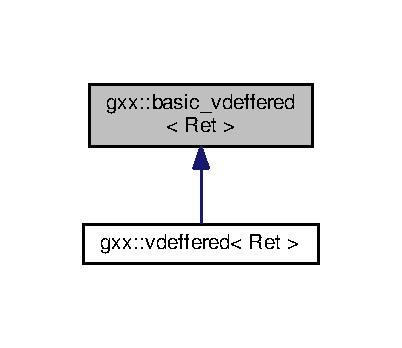
\includegraphics[width=193pt]{structgxx_1_1basic__vdeffered__inherit__graph}
\end{center}
\end{figure}
\subsection*{Public Member Functions}
\begin{DoxyCompactItemize}
\item 
virtual Ret {\bfseries invoke} ()=0\hypertarget{structgxx_1_1basic__vdeffered_a6424707a6c1a3886e509137b8e2d3b5b}{}\label{structgxx_1_1basic__vdeffered_a6424707a6c1a3886e509137b8e2d3b5b}

\end{DoxyCompactItemize}


The documentation for this struct was generated from the following file\+:\begin{DoxyCompactItemize}
\item 
/home/rfmeas/project/gxx/gxx/event/deffered.\+h\end{DoxyCompactItemize}

\hypertarget{classgxx_1_1BasicHashTable}{}\section{gxx\+:\+:Basic\+Hash\+Table Class Reference}
\label{classgxx_1_1BasicHashTable}\index{gxx\+::\+Basic\+Hash\+Table@{gxx\+::\+Basic\+Hash\+Table}}


Inheritance diagram for gxx\+:\+:Basic\+Hash\+Table\+:
\nopagebreak
\begin{figure}[H]
\begin{center}
\leavevmode
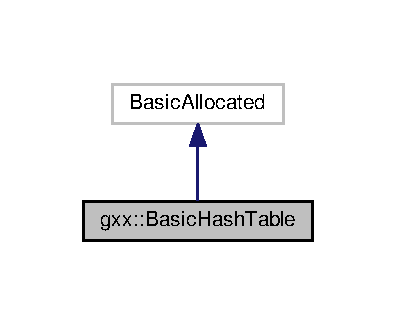
\includegraphics[width=190pt]{classgxx_1_1BasicHashTable__inherit__graph}
\end{center}
\end{figure}


Collaboration diagram for gxx\+:\+:Basic\+Hash\+Table\+:
\nopagebreak
\begin{figure}[H]
\begin{center}
\leavevmode
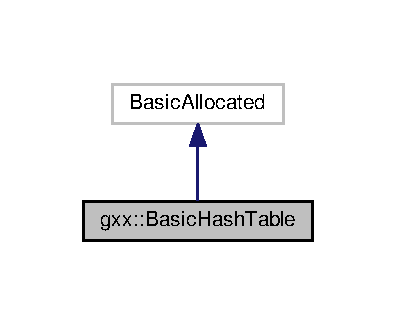
\includegraphics[width=190pt]{classgxx_1_1BasicHashTable__coll__graph}
\end{center}
\end{figure}
\subsection*{Public Member Functions}
\begin{DoxyCompactItemize}
\item 
void {\bfseries reserve} (size\+\_\+t sz)\hypertarget{classgxx_1_1BasicHashTable_a5778618b022b2f41b41ffa798db67dc2}{}\label{classgxx_1_1BasicHashTable_a5778618b022b2f41b41ffa798db67dc2}

\item 
void {\bfseries set\+Strategy} (size\+\_\+t($\ast$func)(\hyperlink{classgxx_1_1BasicHashTable}{Basic\+Hash\+Table} $\ast$))\hypertarget{classgxx_1_1BasicHashTable_af96db4e1ec70d7fd04c92fd842318306}{}\label{classgxx_1_1BasicHashTable_af96db4e1ec70d7fd04c92fd842318306}

\item 
virtual void {\bfseries relocate} (\hyperlink{structhlist__head}{hlist\+\_\+head} $\ast$dst, size\+\_\+t dstsize)=0\hypertarget{classgxx_1_1BasicHashTable_aff55d217bdc65f9987d7bdfbefce7965}{}\label{classgxx_1_1BasicHashTable_aff55d217bdc65f9987d7bdfbefce7965}

\item 
bool {\bfseries is\+\_\+valid} () const \hypertarget{classgxx_1_1BasicHashTable_afe34c280a75f30939d00a17b5036eb87}{}\label{classgxx_1_1BasicHashTable_afe34c280a75f30939d00a17b5036eb87}

\end{DoxyCompactItemize}
\subsection*{Public Attributes}
\begin{DoxyCompactItemize}
\item 
gxx\+::slice$<$ \hyperlink{structhlist__head}{hlist\+\_\+head} $>$ {\bfseries m\+\_\+htable}\hypertarget{classgxx_1_1BasicHashTable_ac34d8677dfeaa91be07dca449dfdf238}{}\label{classgxx_1_1BasicHashTable_ac34d8677dfeaa91be07dca449dfdf238}

\item 
size\+\_\+t {\bfseries m\+\_\+total}\hypertarget{classgxx_1_1BasicHashTable_a039e3aacf067662d55448e90aadf8cd6}{}\label{classgxx_1_1BasicHashTable_a039e3aacf067662d55448e90aadf8cd6}

\item 
size\+\_\+t($\ast$ {\bfseries m\+\_\+strategy} )(\hyperlink{classgxx_1_1BasicHashTable}{Basic\+Hash\+Table} $\ast$)\hypertarget{classgxx_1_1BasicHashTable_ad1bcb87e0a019fcc8a72f862e0f7fde3}{}\label{classgxx_1_1BasicHashTable_ad1bcb87e0a019fcc8a72f862e0f7fde3}

\end{DoxyCompactItemize}


The documentation for this class was generated from the following file\+:\begin{DoxyCompactItemize}
\item 
/home/rfmeas/project/gxx/gxx/container/\+H\+I\+D\+E/hashtable.\+h\end{DoxyCompactItemize}

\hypertarget{structstd_1_1bidirectional__iterator__tag}{}\section{std\+:\+:bidirectional\+\_\+iterator\+\_\+tag Struct Reference}
\label{structstd_1_1bidirectional__iterator__tag}\index{std\+::bidirectional\+\_\+iterator\+\_\+tag@{std\+::bidirectional\+\_\+iterator\+\_\+tag}}


{\ttfamily \#include $<$iterator\+\_\+base\+\_\+types.\+h$>$}



Inheritance diagram for std\+:\+:bidirectional\+\_\+iterator\+\_\+tag\+:
% FIG 0


Collaboration diagram for std\+:\+:bidirectional\+\_\+iterator\+\_\+tag\+:
% FIG 1


\subsection{Detailed Description}
Bidirectional iterators support a superset of forward iterator operations. 

The documentation for this struct was generated from the following file\+:\begin{DoxyCompactItemize}
\item 
/home/rfmeas/project/gxx/gxx/std/iterator\+\_\+base\+\_\+types.\+h\end{DoxyCompactItemize}

\hypertarget{structgxx_1_1bidirectional__iterator__tag}{}\section{gxx\+:\+:bidirectional\+\_\+iterator\+\_\+tag Struct Reference}
\label{structgxx_1_1bidirectional__iterator__tag}\index{gxx\+::bidirectional\+\_\+iterator\+\_\+tag@{gxx\+::bidirectional\+\_\+iterator\+\_\+tag}}


{\ttfamily \#include $<$iterator\+\_\+base\+\_\+types.\+h$>$}



Inheritance diagram for gxx\+:\+:bidirectional\+\_\+iterator\+\_\+tag\+:
% FIG 0


Collaboration diagram for gxx\+:\+:bidirectional\+\_\+iterator\+\_\+tag\+:
% FIG 1


\subsection{Detailed Description}
Bidirectional iterators support a superset of forward iterator operations. 

The documentation for this struct was generated from the following file\+:\begin{DoxyCompactItemize}
\item 
/home/rfmeas/project/gxx/gxx/\+H\+I\+D\+E/iterator\+\_\+base\+\_\+types.\+h\end{DoxyCompactItemize}

\hypertarget{structbig__}{}\section{big\+\_\+ Struct Reference}
\label{structbig__}\index{big\+\_\+@{big\+\_\+}}
\subsection*{Public Attributes}
\begin{DoxyCompactItemize}
\item 
char {\bfseries dummy} \mbox{[}2\mbox{]}\hypertarget{structbig___a08072dda4df56b0f7f3916f97d523f1a}{}\label{structbig___a08072dda4df56b0f7f3916f97d523f1a}

\end{DoxyCompactItemize}


The documentation for this struct was generated from the following file\+:\begin{DoxyCompactItemize}
\item 
/home/rfmeas/project/gxx/gxx/\+H\+I\+D\+E/utility/type\+\_\+traits.\+hpp\end{DoxyCompactItemize}

\hypertarget{structlinalg_1_1op_1_1binary__and}{}\section{linalg\+:\+:op\+:\+:binary\+\_\+and$<$ T $>$ Struct Template Reference}
\label{structlinalg_1_1op_1_1binary__and}\index{linalg\+::op\+::binary\+\_\+and$<$ T $>$@{linalg\+::op\+::binary\+\_\+and$<$ T $>$}}
\subsection*{Public Member Functions}
\begin{DoxyCompactItemize}
\item 
constexpr auto {\bfseries operator()} (T l, T r) const -\/$>$ decltype(l \&r)\hypertarget{structlinalg_1_1op_1_1binary__and_a60697f000860b6e5b24465575e308a72}{}\label{structlinalg_1_1op_1_1binary__and_a60697f000860b6e5b24465575e308a72}

\end{DoxyCompactItemize}


The documentation for this struct was generated from the following file\+:\begin{DoxyCompactItemize}
\item 
/home/rfmeas/project/gxx/gxx/math/linalg.\+h\end{DoxyCompactItemize}

\hypertarget{classgxx_1_1archive_1_1binary__deserializer__basic}{}\section{gxx\+:\+:archive\+:\+:binary\+\_\+deserializer\+\_\+basic Class Reference}
\label{classgxx_1_1archive_1_1binary__deserializer__basic}\index{gxx\+::archive\+::binary\+\_\+deserializer\+\_\+basic@{gxx\+::archive\+::binary\+\_\+deserializer\+\_\+basic}}


Inheritance diagram for gxx\+:\+:archive\+:\+:binary\+\_\+deserializer\+\_\+basic\+:
\nopagebreak
\begin{figure}[H]
\begin{center}
\leavevmode
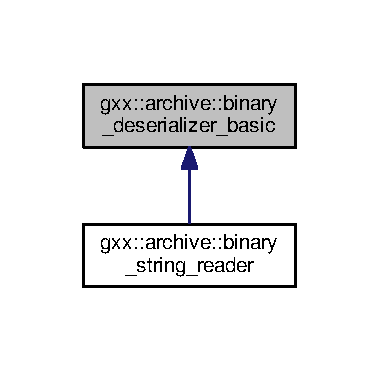
\includegraphics[width=182pt]{classgxx_1_1archive_1_1binary__deserializer__basic__inherit__graph}
\end{center}
\end{figure}
\subsection*{Public Member Functions}
\begin{DoxyCompactItemize}
\item 
{\footnotesize template$<$typename T $>$ }\\void {\bfseries operator\&} (T \&\&obj)\hypertarget{classgxx_1_1archive_1_1binary__deserializer__basic_a5bf9567e3c11621c442b0fb4f00a46b1}{}\label{classgxx_1_1archive_1_1binary__deserializer__basic_a5bf9567e3c11621c442b0fb4f00a46b1}

\item 
virtual void {\bfseries load\+\_\+data} (char $\ast$dat, uint16\+\_\+t sz)=0\hypertarget{classgxx_1_1archive_1_1binary__deserializer__basic_aabcb28260ba2724420125e3b397b5ce7}{}\label{classgxx_1_1archive_1_1binary__deserializer__basic_aabcb28260ba2724420125e3b397b5ce7}

\item 
void {\bfseries do\+\_\+data} (char $\ast$dat, uint16\+\_\+t sz)\hypertarget{classgxx_1_1archive_1_1binary__deserializer__basic_adee825c6ee4e1f532a82feb183cd54a8}{}\label{classgxx_1_1archive_1_1binary__deserializer__basic_adee825c6ee4e1f532a82feb183cd54a8}

\item 
void {\bfseries load} (char $\ast$dat, uint16\+\_\+t maxsz)\hypertarget{classgxx_1_1archive_1_1binary__deserializer__basic_aa528759587f412e22f7e8cd023e4adf0}{}\label{classgxx_1_1archive_1_1binary__deserializer__basic_aa528759587f412e22f7e8cd023e4adf0}

\item 
void {\bfseries load} (char \&i)\hypertarget{classgxx_1_1archive_1_1binary__deserializer__basic_a0835910d47a138f8bf64f7928afec0fa}{}\label{classgxx_1_1archive_1_1binary__deserializer__basic_a0835910d47a138f8bf64f7928afec0fa}

\item 
void {\bfseries load} (short \&i)\hypertarget{classgxx_1_1archive_1_1binary__deserializer__basic_aadce970dc3f550e0c5bebedf6740b1a8}{}\label{classgxx_1_1archive_1_1binary__deserializer__basic_aadce970dc3f550e0c5bebedf6740b1a8}

\item 
void {\bfseries load} (int \&i)\hypertarget{classgxx_1_1archive_1_1binary__deserializer__basic_a88bfb7e4840592801788cf0f31d8e76e}{}\label{classgxx_1_1archive_1_1binary__deserializer__basic_a88bfb7e4840592801788cf0f31d8e76e}

\item 
void {\bfseries load} (long \&i)\hypertarget{classgxx_1_1archive_1_1binary__deserializer__basic_ab861e97ef71acc80823d293c55d971c8}{}\label{classgxx_1_1archive_1_1binary__deserializer__basic_ab861e97ef71acc80823d293c55d971c8}

\item 
void {\bfseries load} (unsigned char \&i)\hypertarget{classgxx_1_1archive_1_1binary__deserializer__basic_a9170ecd3d90d9bdd988bb5882230a429}{}\label{classgxx_1_1archive_1_1binary__deserializer__basic_a9170ecd3d90d9bdd988bb5882230a429}

\item 
void {\bfseries load} (unsigned short \&i)\hypertarget{classgxx_1_1archive_1_1binary__deserializer__basic_af8d432599c25d33adcbbec86fa1b87fa}{}\label{classgxx_1_1archive_1_1binary__deserializer__basic_af8d432599c25d33adcbbec86fa1b87fa}

\item 
void {\bfseries load} (unsigned int \&i)\hypertarget{classgxx_1_1archive_1_1binary__deserializer__basic_a84301b370b91c6c29eb04a217f7ae7ea}{}\label{classgxx_1_1archive_1_1binary__deserializer__basic_a84301b370b91c6c29eb04a217f7ae7ea}

\item 
void {\bfseries load} (unsigned long \&i)\hypertarget{classgxx_1_1archive_1_1binary__deserializer__basic_a74f2bd4d23c49d38918b21e3d3180c84}{}\label{classgxx_1_1archive_1_1binary__deserializer__basic_a74f2bd4d23c49d38918b21e3d3180c84}

\item 
void {\bfseries load} (unsigned long long \&i)\hypertarget{classgxx_1_1archive_1_1binary__deserializer__basic_ae8f764d8e15d1b112e42e0505235285d}{}\label{classgxx_1_1archive_1_1binary__deserializer__basic_ae8f764d8e15d1b112e42e0505235285d}

\item 
void {\bfseries load} (float \&i)\hypertarget{classgxx_1_1archive_1_1binary__deserializer__basic_a0b069742d73746fc056670a0e71baa1e}{}\label{classgxx_1_1archive_1_1binary__deserializer__basic_a0b069742d73746fc056670a0e71baa1e}

\item 
void {\bfseries load} (double \&i)\hypertarget{classgxx_1_1archive_1_1binary__deserializer__basic_ac14166dee2a76b5a0f88e2058b459af4}{}\label{classgxx_1_1archive_1_1binary__deserializer__basic_ac14166dee2a76b5a0f88e2058b459af4}

\item 
void {\bfseries load} (long double \&i)\hypertarget{classgxx_1_1archive_1_1binary__deserializer__basic_a109528082168ec879a19e7635c281cb1}{}\label{classgxx_1_1archive_1_1binary__deserializer__basic_a109528082168ec879a19e7635c281cb1}

\item 
{\footnotesize template$<$typename T $>$ }\\void {\bfseries load} (T \&\&ref)\hypertarget{classgxx_1_1archive_1_1binary__deserializer__basic_a3115894844b9d90039b1bd5383d23843}{}\label{classgxx_1_1archive_1_1binary__deserializer__basic_a3115894844b9d90039b1bd5383d23843}

\end{DoxyCompactItemize}


The documentation for this class was generated from the following file\+:\begin{DoxyCompactItemize}
\item 
/home/rfmeas/project/gxx/gxx/serialize/serialize.\+h\end{DoxyCompactItemize}

\hypertarget{classgxx_1_1serialize_1_1binary__loader}{}\section{gxx\+:\+:serialize\+:\+:binary\+\_\+loader Class Reference}
\label{classgxx_1_1serialize_1_1binary__loader}\index{gxx\+::serialize\+::binary\+\_\+loader@{gxx\+::serialize\+::binary\+\_\+loader}}
\subsection*{Public Member Functions}
\begin{DoxyCompactItemize}
\item 
{\bfseries binary\+\_\+loader} (\hyperlink{classgxx_1_1buffer}{gxx\+::buffer} buf)\hypertarget{classgxx_1_1serialize_1_1binary__loader_ab2f5fe7dae09fbd8bcff38d3bcf316ac}{}\label{classgxx_1_1serialize_1_1binary__loader_ab2f5fe7dae09fbd8bcff38d3bcf316ac}

\item 
{\footnotesize template$<$typename T $>$ }\\void {\bfseries operator\&} (T \&obj)\hypertarget{classgxx_1_1serialize_1_1binary__loader_ae5cbcff20c75f9278b3fa402764be1a2}{}\label{classgxx_1_1serialize_1_1binary__loader_ae5cbcff20c75f9278b3fa402764be1a2}

\item 
{\footnotesize template$<$typename T $>$ }\\void {\bfseries load} (T \&obj)\hypertarget{classgxx_1_1serialize_1_1binary__loader_a69bc4b2cb1bd677470b4f9dbe929f265}{}\label{classgxx_1_1serialize_1_1binary__loader_a69bc4b2cb1bd677470b4f9dbe929f265}

\item 
void {\bfseries load} (int \&i)\hypertarget{classgxx_1_1serialize_1_1binary__loader_aadffa2611b810a4040d0917252c9b5ee}{}\label{classgxx_1_1serialize_1_1binary__loader_aadffa2611b810a4040d0917252c9b5ee}

\end{DoxyCompactItemize}


The documentation for this class was generated from the following file\+:\begin{DoxyCompactItemize}
\item 
/home/rfmeas/project/gxx/gxx/\+H\+I\+D\+E/transport/serialize.\+h\end{DoxyCompactItemize}

\hypertarget{structlinalg_1_1op_1_1binary__not}{}\section{linalg\+:\+:op\+:\+:binary\+\_\+not$<$ T $>$ Struct Template Reference}
\label{structlinalg_1_1op_1_1binary__not}\index{linalg\+::op\+::binary\+\_\+not$<$ T $>$@{linalg\+::op\+::binary\+\_\+not$<$ T $>$}}
\subsection*{Public Member Functions}
\begin{DoxyCompactItemize}
\item 
constexpr auto {\bfseries operator()} (T r) const -\/$>$ decltype(+r)\hypertarget{structlinalg_1_1op_1_1binary__not_aea163eb0110bd7ddd33f483f9b5379db}{}\label{structlinalg_1_1op_1_1binary__not_aea163eb0110bd7ddd33f483f9b5379db}

\end{DoxyCompactItemize}


The documentation for this struct was generated from the following file\+:\begin{DoxyCompactItemize}
\item 
/home/rfmeas/project/gxx/gxx/math/linalg.\+h\end{DoxyCompactItemize}

\hypertarget{structlinalg_1_1op_1_1binary__or}{}\section{linalg\+:\+:op\+:\+:binary\+\_\+or$<$ T $>$ Struct Template Reference}
\label{structlinalg_1_1op_1_1binary__or}\index{linalg\+::op\+::binary\+\_\+or$<$ T $>$@{linalg\+::op\+::binary\+\_\+or$<$ T $>$}}
\subsection*{Public Member Functions}
\begin{DoxyCompactItemize}
\item 
constexpr auto {\bfseries operator()} (T l, T r) const -\/$>$ decltype(l$\vert$r)\hypertarget{structlinalg_1_1op_1_1binary__or_a87e34114f8a7c5868cf7baebc67a891c}{}\label{structlinalg_1_1op_1_1binary__or_a87e34114f8a7c5868cf7baebc67a891c}

\end{DoxyCompactItemize}


The documentation for this struct was generated from the following file\+:\begin{DoxyCompactItemize}
\item 
/home/rfmeas/project/gxx/gxx/math/linalg.\+h\end{DoxyCompactItemize}

\hypertarget{classgxx_1_1serialize_1_1binary__saver}{}\section{gxx\+:\+:serialize\+:\+:binary\+\_\+saver Class Reference}
\label{classgxx_1_1serialize_1_1binary__saver}\index{gxx\+::serialize\+::binary\+\_\+saver@{gxx\+::serialize\+::binary\+\_\+saver}}
\subsection*{Public Member Functions}
\begin{DoxyCompactItemize}
\item 
{\bfseries binary\+\_\+saver} (\hyperlink{classgxx_1_1buffer}{gxx\+::buffer} buf)\hypertarget{classgxx_1_1serialize_1_1binary__saver_a4bca01b1beea967c98d8653a7fd49125}{}\label{classgxx_1_1serialize_1_1binary__saver_a4bca01b1beea967c98d8653a7fd49125}

\item 
{\footnotesize template$<$typename T $>$ }\\void {\bfseries operator\&} (T \&obj)\hypertarget{classgxx_1_1serialize_1_1binary__saver_abb39ead1609adaf314204114bfc31431}{}\label{classgxx_1_1serialize_1_1binary__saver_abb39ead1609adaf314204114bfc31431}

\item 
{\footnotesize template$<$typename T $>$ }\\void {\bfseries dump} (T \&obj)\hypertarget{classgxx_1_1serialize_1_1binary__saver_ac3feded47f584f858c15fcf3a61277ca}{}\label{classgxx_1_1serialize_1_1binary__saver_ac3feded47f584f858c15fcf3a61277ca}

\item 
void {\bfseries dump} (short i)\hypertarget{classgxx_1_1serialize_1_1binary__saver_a86018a16014db77e82f13bc2dd698ecb}{}\label{classgxx_1_1serialize_1_1binary__saver_a86018a16014db77e82f13bc2dd698ecb}

\item 
void {\bfseries dump} (int i)\hypertarget{classgxx_1_1serialize_1_1binary__saver_a088c428ea3dcbc5642df17700b4437e2}{}\label{classgxx_1_1serialize_1_1binary__saver_a088c428ea3dcbc5642df17700b4437e2}

\item 
void {\bfseries dump} (long i)\hypertarget{classgxx_1_1serialize_1_1binary__saver_a56cefadc087e509e1a2bd89411f5c360}{}\label{classgxx_1_1serialize_1_1binary__saver_a56cefadc087e509e1a2bd89411f5c360}

\item 
void {\bfseries dump} (long long i)\hypertarget{classgxx_1_1serialize_1_1binary__saver_a1bbe03087c55aee7a535a4f0d6cfddc2}{}\label{classgxx_1_1serialize_1_1binary__saver_a1bbe03087c55aee7a535a4f0d6cfddc2}

\item 
\hyperlink{classgxx_1_1buffer}{gxx\+::buffer} {\bfseries getbuf} ()\hypertarget{classgxx_1_1serialize_1_1binary__saver_ac06cff44e0b6e33abebeccae82d938ef}{}\label{classgxx_1_1serialize_1_1binary__saver_ac06cff44e0b6e33abebeccae82d938ef}

\end{DoxyCompactItemize}


The documentation for this class was generated from the following file\+:\begin{DoxyCompactItemize}
\item 
/home/rfmeas/project/gxx/gxx/\+H\+I\+D\+E/transport/serialize.\+h\end{DoxyCompactItemize}

\hypertarget{classgxx_1_1archive_1_1binary__serializer__basic}{}\section{gxx\+:\+:archive\+:\+:binary\+\_\+serializer\+\_\+basic Class Reference}
\label{classgxx_1_1archive_1_1binary__serializer__basic}\index{gxx\+::archive\+::binary\+\_\+serializer\+\_\+basic@{gxx\+::archive\+::binary\+\_\+serializer\+\_\+basic}}


Inheritance diagram for gxx\+:\+:archive\+:\+:binary\+\_\+serializer\+\_\+basic\+:
\nopagebreak
\begin{figure}[H]
\begin{center}
\leavevmode
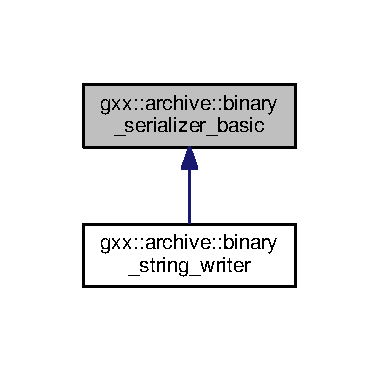
\includegraphics[width=182pt]{classgxx_1_1archive_1_1binary__serializer__basic__inherit__graph}
\end{center}
\end{figure}
\subsection*{Public Member Functions}
\begin{DoxyCompactItemize}
\item 
{\footnotesize template$<$typename T $>$ }\\void {\bfseries operator\&} (const T \&obj)\hypertarget{classgxx_1_1archive_1_1binary__serializer__basic_a738d83d711c6b75db269d1dab67c07fb}{}\label{classgxx_1_1archive_1_1binary__serializer__basic_a738d83d711c6b75db269d1dab67c07fb}

\item 
virtual void {\bfseries dump\+\_\+data} (const char $\ast$dat, uint16\+\_\+t sz)=0\hypertarget{classgxx_1_1archive_1_1binary__serializer__basic_a9a6ee8baa50e229dd7635452ce183b18}{}\label{classgxx_1_1archive_1_1binary__serializer__basic_a9a6ee8baa50e229dd7635452ce183b18}

\item 
void {\bfseries do\+\_\+data} (const char $\ast$dat, uint16\+\_\+t sz)\hypertarget{classgxx_1_1archive_1_1binary__serializer__basic_a30337c9dac545308bf37a6df5c56cda2}{}\label{classgxx_1_1archive_1_1binary__serializer__basic_a30337c9dac545308bf37a6df5c56cda2}

\item 
void {\bfseries dump} (const char $\ast$dat, uint16\+\_\+t sz)\hypertarget{classgxx_1_1archive_1_1binary__serializer__basic_aafbd976ea46283071a75b6c748d9c933}{}\label{classgxx_1_1archive_1_1binary__serializer__basic_aafbd976ea46283071a75b6c748d9c933}

\item 
void {\bfseries dump} (char i)\hypertarget{classgxx_1_1archive_1_1binary__serializer__basic_aac1b672e27662d6e950918919445e427}{}\label{classgxx_1_1archive_1_1binary__serializer__basic_aac1b672e27662d6e950918919445e427}

\item 
void {\bfseries dump} (short i)\hypertarget{classgxx_1_1archive_1_1binary__serializer__basic_ae19a3849d71be30f66920fb1e53c702e}{}\label{classgxx_1_1archive_1_1binary__serializer__basic_ae19a3849d71be30f66920fb1e53c702e}

\item 
void {\bfseries dump} (int i)\hypertarget{classgxx_1_1archive_1_1binary__serializer__basic_a5d3bc99853697cd949a3d0a0d9057553}{}\label{classgxx_1_1archive_1_1binary__serializer__basic_a5d3bc99853697cd949a3d0a0d9057553}

\item 
void {\bfseries dump} (long i)\hypertarget{classgxx_1_1archive_1_1binary__serializer__basic_aa177f21a942782ecee23338b69ede294}{}\label{classgxx_1_1archive_1_1binary__serializer__basic_aa177f21a942782ecee23338b69ede294}

\item 
void {\bfseries dump} (unsigned char i)\hypertarget{classgxx_1_1archive_1_1binary__serializer__basic_af2472269cba3166850ba7b3009b10a89}{}\label{classgxx_1_1archive_1_1binary__serializer__basic_af2472269cba3166850ba7b3009b10a89}

\item 
void {\bfseries dump} (unsigned short i)\hypertarget{classgxx_1_1archive_1_1binary__serializer__basic_a7bf73357b5f2099d29ca8876c06384a9}{}\label{classgxx_1_1archive_1_1binary__serializer__basic_a7bf73357b5f2099d29ca8876c06384a9}

\item 
void {\bfseries dump} (unsigned int i)\hypertarget{classgxx_1_1archive_1_1binary__serializer__basic_aa3690cb7560d88fe7c41627984c0c8f7}{}\label{classgxx_1_1archive_1_1binary__serializer__basic_aa3690cb7560d88fe7c41627984c0c8f7}

\item 
void {\bfseries dump} (unsigned long i)\hypertarget{classgxx_1_1archive_1_1binary__serializer__basic_a12778c4c2fab2b46be4c2c23144dcf27}{}\label{classgxx_1_1archive_1_1binary__serializer__basic_a12778c4c2fab2b46be4c2c23144dcf27}

\item 
void {\bfseries dump} (unsigned long long i)\hypertarget{classgxx_1_1archive_1_1binary__serializer__basic_a399ba6ac58658a735209d9a1e4f53a52}{}\label{classgxx_1_1archive_1_1binary__serializer__basic_a399ba6ac58658a735209d9a1e4f53a52}

\item 
void {\bfseries dump} (float i)\hypertarget{classgxx_1_1archive_1_1binary__serializer__basic_a16af5ad71c579a5c17e9d78315f4613e}{}\label{classgxx_1_1archive_1_1binary__serializer__basic_a16af5ad71c579a5c17e9d78315f4613e}

\item 
void {\bfseries dump} (double i)\hypertarget{classgxx_1_1archive_1_1binary__serializer__basic_a03b6fe9f681d4a4370b97ee9150da506}{}\label{classgxx_1_1archive_1_1binary__serializer__basic_a03b6fe9f681d4a4370b97ee9150da506}

\item 
void {\bfseries dump} (long double i)\hypertarget{classgxx_1_1archive_1_1binary__serializer__basic_a322a38bbac67825232b635474d9167d6}{}\label{classgxx_1_1archive_1_1binary__serializer__basic_a322a38bbac67825232b635474d9167d6}

\item 
{\footnotesize template$<$typename T $>$ }\\void {\bfseries dump} (const T \&ref)\hypertarget{classgxx_1_1archive_1_1binary__serializer__basic_ae7baa8542e7e32ddd0bf25ec845c031a}{}\label{classgxx_1_1archive_1_1binary__serializer__basic_ae7baa8542e7e32ddd0bf25ec845c031a}

\end{DoxyCompactItemize}


The documentation for this class was generated from the following file\+:\begin{DoxyCompactItemize}
\item 
/home/rfmeas/project/gxx/gxx/serialize/serialize.\+h\end{DoxyCompactItemize}

\hypertarget{structhalf__float_1_1detail_1_1binary__specialized}{}\section{half\+\_\+float\+:\+:detail\+:\+:binary\+\_\+specialized$<$ T, U $>$ Struct Template Reference}
\label{structhalf__float_1_1detail_1_1binary__specialized}\index{half\+\_\+float\+::detail\+::binary\+\_\+specialized$<$ T, U $>$@{half\+\_\+float\+::detail\+::binary\+\_\+specialized$<$ T, U $>$}}


{\ttfamily \#include $<$half.\+h$>$}

\subsection*{Static Public Member Functions}
\begin{DoxyCompactItemize}
\item 
static \hyperlink{structhalf__float_1_1detail_1_1expr}{expr} \hyperlink{structhalf__float_1_1detail_1_1binary__specialized_afb9ec4bebd2df86f570d20a6e7c6392f}{fmin} (float x, float y)
\item 
static \hyperlink{structhalf__float_1_1detail_1_1expr}{expr} \hyperlink{structhalf__float_1_1detail_1_1binary__specialized_a3d46871722c0a117f1921cc11bf47a89}{fmax} (float x, float y)
\end{DoxyCompactItemize}


\subsection{Detailed Description}
\subsubsection*{template$<$typename T, typename U$>$\\*
struct half\+\_\+float\+::detail\+::binary\+\_\+specialized$<$ T, U $>$}

Wrapper for binary half-\/precision functions needing specialization for individual argument types. 
\begin{DoxyTemplParams}{Template Parameters}
{\em T} & first argument type \\
\hline
{\em U} & first argument type \\
\hline
\end{DoxyTemplParams}


\subsection{Member Function Documentation}
\index{half\+\_\+float\+::detail\+::binary\+\_\+specialized@{half\+\_\+float\+::detail\+::binary\+\_\+specialized}!fmax@{fmax}}
\index{fmax@{fmax}!half\+\_\+float\+::detail\+::binary\+\_\+specialized@{half\+\_\+float\+::detail\+::binary\+\_\+specialized}}
\subsubsection[{\texorpdfstring{fmax(float x, float y)}{fmax(float x, float y)}}]{\setlength{\rightskip}{0pt plus 5cm}template$<$typename T , typename U $>$ static {\bf expr} {\bf half\+\_\+float\+::detail\+::binary\+\_\+specialized}$<$ T, U $>$\+::fmax (
\begin{DoxyParamCaption}
\item[{float}]{x, }
\item[{float}]{y}
\end{DoxyParamCaption}
)\hspace{0.3cm}{\ttfamily [inline]}, {\ttfamily [static]}}\hypertarget{structhalf__float_1_1detail_1_1binary__specialized_a3d46871722c0a117f1921cc11bf47a89}{}\label{structhalf__float_1_1detail_1_1binary__specialized_a3d46871722c0a117f1921cc11bf47a89}
Maximum implementation. 
\begin{DoxyParams}{Parameters}
{\em x} & first operand \\
\hline
{\em y} & second operand \\
\hline
\end{DoxyParams}
\begin{DoxyReturn}{Returns}
maximum value 
\end{DoxyReturn}
\index{half\+\_\+float\+::detail\+::binary\+\_\+specialized@{half\+\_\+float\+::detail\+::binary\+\_\+specialized}!fmin@{fmin}}
\index{fmin@{fmin}!half\+\_\+float\+::detail\+::binary\+\_\+specialized@{half\+\_\+float\+::detail\+::binary\+\_\+specialized}}
\subsubsection[{\texorpdfstring{fmin(float x, float y)}{fmin(float x, float y)}}]{\setlength{\rightskip}{0pt plus 5cm}template$<$typename T , typename U $>$ static {\bf expr} {\bf half\+\_\+float\+::detail\+::binary\+\_\+specialized}$<$ T, U $>$\+::fmin (
\begin{DoxyParamCaption}
\item[{float}]{x, }
\item[{float}]{y}
\end{DoxyParamCaption}
)\hspace{0.3cm}{\ttfamily [inline]}, {\ttfamily [static]}}\hypertarget{structhalf__float_1_1detail_1_1binary__specialized_afb9ec4bebd2df86f570d20a6e7c6392f}{}\label{structhalf__float_1_1detail_1_1binary__specialized_afb9ec4bebd2df86f570d20a6e7c6392f}
Minimum implementation. 
\begin{DoxyParams}{Parameters}
{\em x} & first operand \\
\hline
{\em y} & second operand \\
\hline
\end{DoxyParams}
\begin{DoxyReturn}{Returns}
minimum value 
\end{DoxyReturn}


The documentation for this struct was generated from the following file\+:\begin{DoxyCompactItemize}
\item 
/home/rfmeas/project/gxx/gxx/math/\hyperlink{half_8h}{half.\+h}\end{DoxyCompactItemize}

\hypertarget{structhalf__float_1_1detail_1_1binary__specialized_3_01half_00_01half_01_4}{}\section{half\+\_\+float\+:\+:detail\+:\+:binary\+\_\+specialized$<$ half, half $>$ Struct Template Reference}
\label{structhalf__float_1_1detail_1_1binary__specialized_3_01half_00_01half_01_4}\index{half\+\_\+float\+::detail\+::binary\+\_\+specialized$<$ half, half $>$@{half\+\_\+float\+::detail\+::binary\+\_\+specialized$<$ half, half $>$}}
\subsection*{Static Public Member Functions}
\begin{DoxyCompactItemize}
\item 
static \hyperlink{classhalf__float_1_1half}{half} {\bfseries fmin} (\hyperlink{classhalf__float_1_1half}{half} x, \hyperlink{classhalf__float_1_1half}{half} y)\hypertarget{structhalf__float_1_1detail_1_1binary__specialized_3_01half_00_01half_01_4_a26cf067eeb5a5a7b20d0da1ddade32ad}{}\label{structhalf__float_1_1detail_1_1binary__specialized_3_01half_00_01half_01_4_a26cf067eeb5a5a7b20d0da1ddade32ad}

\item 
static \hyperlink{classhalf__float_1_1half}{half} {\bfseries fmax} (\hyperlink{classhalf__float_1_1half}{half} x, \hyperlink{classhalf__float_1_1half}{half} y)\hypertarget{structhalf__float_1_1detail_1_1binary__specialized_3_01half_00_01half_01_4_a906748ac07462c30c52cfe7145ae307c}{}\label{structhalf__float_1_1detail_1_1binary__specialized_3_01half_00_01half_01_4_a906748ac07462c30c52cfe7145ae307c}

\end{DoxyCompactItemize}


The documentation for this struct was generated from the following file\+:\begin{DoxyCompactItemize}
\item 
/home/rfmeas/project/gxx/gxx/math/\hyperlink{half_8h}{half.\+h}\end{DoxyCompactItemize}

\hypertarget{classgxx_1_1archive_1_1binary__string__reader}{}\section{gxx\+:\+:archive\+:\+:binary\+\_\+string\+\_\+reader Class Reference}
\label{classgxx_1_1archive_1_1binary__string__reader}\index{gxx\+::archive\+::binary\+\_\+string\+\_\+reader@{gxx\+::archive\+::binary\+\_\+string\+\_\+reader}}


Inheritance diagram for gxx\+:\+:archive\+:\+:binary\+\_\+string\+\_\+reader\+:
\nopagebreak
\begin{figure}[H]
\begin{center}
\leavevmode
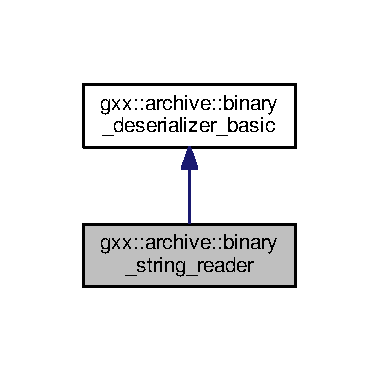
\includegraphics[width=182pt]{classgxx_1_1archive_1_1binary__string__reader__inherit__graph}
\end{center}
\end{figure}


Collaboration diagram for gxx\+:\+:archive\+:\+:binary\+\_\+string\+\_\+reader\+:
\nopagebreak
\begin{figure}[H]
\begin{center}
\leavevmode
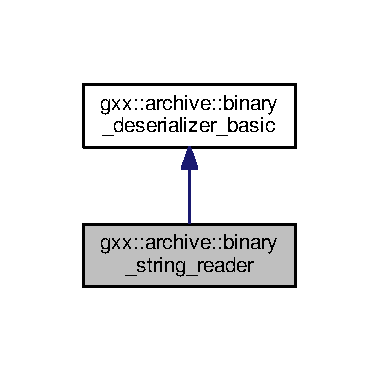
\includegraphics[width=182pt]{classgxx_1_1archive_1_1binary__string__reader__coll__graph}
\end{center}
\end{figure}
\subsection*{Public Member Functions}
\begin{DoxyCompactItemize}
\item 
void {\bfseries load\+\_\+data} (char $\ast$dat, uint16\+\_\+t size) override\hypertarget{classgxx_1_1archive_1_1binary__string__reader_a581a1363185e7720c1bce91a49af42fe}{}\label{classgxx_1_1archive_1_1binary__string__reader_a581a1363185e7720c1bce91a49af42fe}

\item 
{\bfseries binary\+\_\+string\+\_\+reader} (const std\+::string \&str)\hypertarget{classgxx_1_1archive_1_1binary__string__reader_a3b71d311c3be2e6d68ca09991425c420}{}\label{classgxx_1_1archive_1_1binary__string__reader_a3b71d311c3be2e6d68ca09991425c420}

\end{DoxyCompactItemize}
\subsection*{Public Attributes}
\begin{DoxyCompactItemize}
\item 
std\+::istringstream {\bfseries stream}\hypertarget{classgxx_1_1archive_1_1binary__string__reader_a91e8cf3dcd508ab78708594277da462e}{}\label{classgxx_1_1archive_1_1binary__string__reader_a91e8cf3dcd508ab78708594277da462e}

\end{DoxyCompactItemize}


The documentation for this class was generated from the following file\+:\begin{DoxyCompactItemize}
\item 
/home/rfmeas/project/gxx/gxx/serialize/serialize.\+h\end{DoxyCompactItemize}

\hypertarget{classgxx_1_1archive_1_1binary__string__writer}{}\section{gxx\+:\+:archive\+:\+:binary\+\_\+string\+\_\+writer Class Reference}
\label{classgxx_1_1archive_1_1binary__string__writer}\index{gxx\+::archive\+::binary\+\_\+string\+\_\+writer@{gxx\+::archive\+::binary\+\_\+string\+\_\+writer}}


Inheritance diagram for gxx\+:\+:archive\+:\+:binary\+\_\+string\+\_\+writer\+:
\nopagebreak
\begin{figure}[H]
\begin{center}
\leavevmode
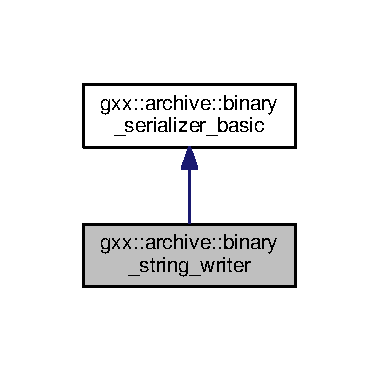
\includegraphics[width=182pt]{classgxx_1_1archive_1_1binary__string__writer__inherit__graph}
\end{center}
\end{figure}


Collaboration diagram for gxx\+:\+:archive\+:\+:binary\+\_\+string\+\_\+writer\+:
\nopagebreak
\begin{figure}[H]
\begin{center}
\leavevmode
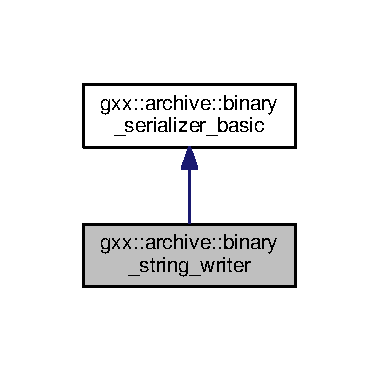
\includegraphics[width=182pt]{classgxx_1_1archive_1_1binary__string__writer__coll__graph}
\end{center}
\end{figure}
\subsection*{Public Member Functions}
\begin{DoxyCompactItemize}
\item 
void {\bfseries dump\+\_\+data} (const char $\ast$dat, uint16\+\_\+t size) override\hypertarget{classgxx_1_1archive_1_1binary__string__writer_ae4512b00c3764d825089d4b36fd56115}{}\label{classgxx_1_1archive_1_1binary__string__writer_ae4512b00c3764d825089d4b36fd56115}

\item 
{\bfseries binary\+\_\+string\+\_\+writer} (std\+::string \&str)\hypertarget{classgxx_1_1archive_1_1binary__string__writer_a99ad4c8bb49e1e8ebc0009a4be8e61d0}{}\label{classgxx_1_1archive_1_1binary__string__writer_a99ad4c8bb49e1e8ebc0009a4be8e61d0}

\end{DoxyCompactItemize}
\subsection*{Public Attributes}
\begin{DoxyCompactItemize}
\item 
std\+::string \& {\bfseries sstr}\hypertarget{classgxx_1_1archive_1_1binary__string__writer_af2aa4f19499b335fadcb430a43a353eb}{}\label{classgxx_1_1archive_1_1binary__string__writer_af2aa4f19499b335fadcb430a43a353eb}

\end{DoxyCompactItemize}


The documentation for this class was generated from the following file\+:\begin{DoxyCompactItemize}
\item 
/home/rfmeas/project/gxx/gxx/serialize/serialize.\+h\end{DoxyCompactItemize}

\hypertarget{structhalf__float_1_1detail_1_1binary__t}{}\section{half\+\_\+float\+:\+:detail\+:\+:binary\+\_\+t Struct Reference}
\label{structhalf__float_1_1detail_1_1binary__t}\index{half\+\_\+float\+::detail\+::binary\+\_\+t@{half\+\_\+float\+::detail\+::binary\+\_\+t}}


Tag type for binary construction.  




{\ttfamily \#include $<$half.\+h$>$}



\subsection{Detailed Description}
Tag type for binary construction. 

The documentation for this struct was generated from the following file\+:\begin{DoxyCompactItemize}
\item 
/home/rfmeas/project/gxx/gxx/math/\hyperlink{half_8h}{half.\+h}\end{DoxyCompactItemize}

\hypertarget{structlinalg_1_1op_1_1binary__xor}{}\section{linalg\+:\+:op\+:\+:binary\+\_\+xor$<$ T $>$ Struct Template Reference}
\label{structlinalg_1_1op_1_1binary__xor}\index{linalg\+::op\+::binary\+\_\+xor$<$ T $>$@{linalg\+::op\+::binary\+\_\+xor$<$ T $>$}}
\subsection*{Public Member Functions}
\begin{DoxyCompactItemize}
\item 
constexpr auto {\bfseries operator()} (T l, T r) const -\/$>$ decltype(l$^\wedge$r)\hypertarget{structlinalg_1_1op_1_1binary__xor_a8fafc8173f9d09ab122c5323a3dacde5}{}\label{structlinalg_1_1op_1_1binary__xor_a8fafc8173f9d09ab122c5323a3dacde5}

\end{DoxyCompactItemize}


The documentation for this struct was generated from the following file\+:\begin{DoxyCompactItemize}
\item 
/home/rfmeas/project/gxx/gxx/math/linalg.\+h\end{DoxyCompactItemize}

\hypertarget{classgxx_1_1rpc_1_1bincall}{}\section{gxx\+:\+:rpc\+:\+:bincall$<$ Delegate $>$ Class Template Reference}
\label{classgxx_1_1rpc_1_1bincall}\index{gxx\+::rpc\+::bincall$<$ Delegate $>$@{gxx\+::rpc\+::bincall$<$ Delegate $>$}}


The documentation for this class was generated from the following file\+:\begin{DoxyCompactItemize}
\item 
/home/rfmeas/project/gxx/gxx/rpc/bincall.\+h\end{DoxyCompactItemize}

\hypertarget{classgxx_1_1rpc_1_1bincall_3_01gxx_1_1delegate_3_01R_00_01T0_00_01T1_00_01T2_01_4_01_4}{}\section{gxx\+:\+:rpc\+:\+:bincall$<$ gxx\+:\+:delegate$<$ R, T0, T1, T2 $>$ $>$ Class Template Reference}
\label{classgxx_1_1rpc_1_1bincall_3_01gxx_1_1delegate_3_01R_00_01T0_00_01T1_00_01T2_01_4_01_4}\index{gxx\+::rpc\+::bincall$<$ gxx\+::delegate$<$ R, T0, T1, T2 $>$ $>$@{gxx\+::rpc\+::bincall$<$ gxx\+::delegate$<$ R, T0, T1, T2 $>$ $>$}}


Inheritance diagram for gxx\+:\+:rpc\+:\+:bincall$<$ gxx\+:\+:delegate$<$ R, T0, T1, T2 $>$ $>$\+:
% FIG 0


Collaboration diagram for gxx\+:\+:rpc\+:\+:bincall$<$ gxx\+:\+:delegate$<$ R, T0, T1, T2 $>$ $>$\+:
% FIG 1
\subsection*{Public Member Functions}
\begin{DoxyCompactItemize}
\item 
{\bfseries bincall} (\hyperlink{classgxx_1_1delegate}{gxx\+::delegate}$<$ rpcresult$<$ R $>$, T0, T1, T2 $>$ dlg)\hypertarget{classgxx_1_1rpc_1_1bincall_3_01gxx_1_1delegate_3_01R_00_01T0_00_01T1_00_01T2_01_4_01_4_add91072889278f4ddd8bc3fdb3160b0d}{}\label{classgxx_1_1rpc_1_1bincall_3_01gxx_1_1delegate_3_01R_00_01T0_00_01T1_00_01T2_01_4_01_4_add91072889278f4ddd8bc3fdb3160b0d}

\item 
status {\bfseries invoke} (gxx\+::archive\+::binary\+\_\+reader \&keeper, gxx\+::archive\+::binary\+\_\+writer \&\hyperlink{classgxx_1_1writer}{writer}) override\hypertarget{classgxx_1_1rpc_1_1bincall_3_01gxx_1_1delegate_3_01R_00_01T0_00_01T1_00_01T2_01_4_01_4_a07f96fda38a384a9ffacdbcb4c2c2493}{}\label{classgxx_1_1rpc_1_1bincall_3_01gxx_1_1delegate_3_01R_00_01T0_00_01T1_00_01T2_01_4_01_4_a07f96fda38a384a9ffacdbcb4c2c2493}

\end{DoxyCompactItemize}


The documentation for this class was generated from the following file\+:\begin{DoxyCompactItemize}
\item 
/home/rfmeas/project/gxx/gxx/rpc/bincall.\+h\end{DoxyCompactItemize}

\hypertarget{classgxx_1_1rpc_1_1bincall_3_01gxx_1_1delegate_3_01rpcresult_3_01R_01_4_01_4_01_4}{}\section{gxx\+:\+:rpc\+:\+:bincall$<$ gxx\+:\+:delegate$<$ rpcresult$<$ R $>$ $>$ $>$ Class Template Reference}
\label{classgxx_1_1rpc_1_1bincall_3_01gxx_1_1delegate_3_01rpcresult_3_01R_01_4_01_4_01_4}\index{gxx\+::rpc\+::bincall$<$ gxx\+::delegate$<$ rpcresult$<$ R $>$ $>$ $>$@{gxx\+::rpc\+::bincall$<$ gxx\+::delegate$<$ rpcresult$<$ R $>$ $>$ $>$}}


Inheritance diagram for gxx\+:\+:rpc\+:\+:bincall$<$ gxx\+:\+:delegate$<$ rpcresult$<$ R $>$ $>$ $>$\+:
\nopagebreak
\begin{figure}[H]
\begin{center}
\leavevmode
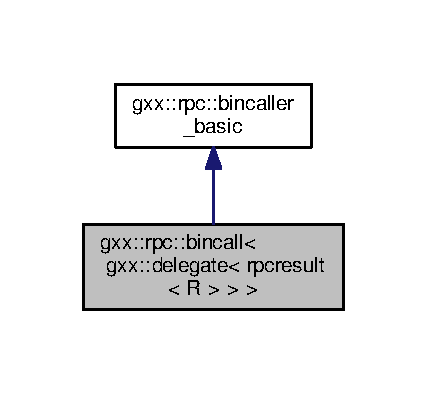
\includegraphics[width=205pt]{classgxx_1_1rpc_1_1bincall_3_01gxx_1_1delegate_3_01rpcresult_3_01R_01_4_01_4_01_4__inherit__graph}
\end{center}
\end{figure}


Collaboration diagram for gxx\+:\+:rpc\+:\+:bincall$<$ gxx\+:\+:delegate$<$ rpcresult$<$ R $>$ $>$ $>$\+:
\nopagebreak
\begin{figure}[H]
\begin{center}
\leavevmode
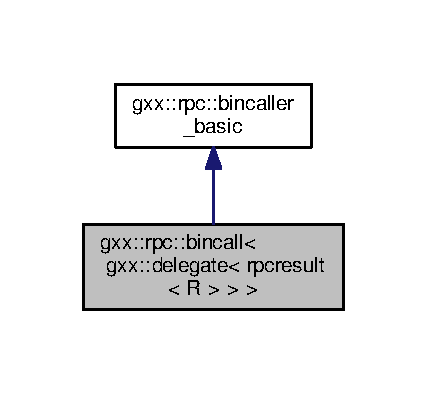
\includegraphics[width=205pt]{classgxx_1_1rpc_1_1bincall_3_01gxx_1_1delegate_3_01rpcresult_3_01R_01_4_01_4_01_4__coll__graph}
\end{center}
\end{figure}
\subsection*{Public Member Functions}
\begin{DoxyCompactItemize}
\item 
{\bfseries bincall} (\hyperlink{classgxx_1_1delegate}{gxx\+::delegate}$<$ rpcresult$<$ R $>$$>$ dlg)\hypertarget{classgxx_1_1rpc_1_1bincall_3_01gxx_1_1delegate_3_01rpcresult_3_01R_01_4_01_4_01_4_a6d37f5aa305b2b1ff57baa06379cc2cd}{}\label{classgxx_1_1rpc_1_1bincall_3_01gxx_1_1delegate_3_01rpcresult_3_01R_01_4_01_4_01_4_a6d37f5aa305b2b1ff57baa06379cc2cd}

\item 
status {\bfseries invoke} (gxx\+::archive\+::binary\+\_\+reader \&keeper, gxx\+::archive\+::binary\+\_\+writer \&\hyperlink{classgxx_1_1writer}{writer}) override\hypertarget{classgxx_1_1rpc_1_1bincall_3_01gxx_1_1delegate_3_01rpcresult_3_01R_01_4_01_4_01_4_ae978cb5bffe2eb887007ea3b27c5efda}{}\label{classgxx_1_1rpc_1_1bincall_3_01gxx_1_1delegate_3_01rpcresult_3_01R_01_4_01_4_01_4_ae978cb5bffe2eb887007ea3b27c5efda}

\end{DoxyCompactItemize}


The documentation for this class was generated from the following file\+:\begin{DoxyCompactItemize}
\item 
/home/rfmeas/project/gxx/gxx/rpc/bincall.\+h\end{DoxyCompactItemize}

\hypertarget{classgxx_1_1rpc_1_1bincall_3_01gxx_1_1delegate_3_01rpcresult_3_01R_01_4_00_01T0_01_4_01_4}{}\section{gxx\+:\+:rpc\+:\+:bincall$<$ gxx\+:\+:delegate$<$ rpcresult$<$ R $>$, T0 $>$ $>$ Class Template Reference}
\label{classgxx_1_1rpc_1_1bincall_3_01gxx_1_1delegate_3_01rpcresult_3_01R_01_4_00_01T0_01_4_01_4}\index{gxx\+::rpc\+::bincall$<$ gxx\+::delegate$<$ rpcresult$<$ R $>$, T0 $>$ $>$@{gxx\+::rpc\+::bincall$<$ gxx\+::delegate$<$ rpcresult$<$ R $>$, T0 $>$ $>$}}


Inheritance diagram for gxx\+:\+:rpc\+:\+:bincall$<$ gxx\+:\+:delegate$<$ rpcresult$<$ R $>$, T0 $>$ $>$\+:
% FIG 0


Collaboration diagram for gxx\+:\+:rpc\+:\+:bincall$<$ gxx\+:\+:delegate$<$ rpcresult$<$ R $>$, T0 $>$ $>$\+:
% FIG 1
\subsection*{Public Member Functions}
\begin{DoxyCompactItemize}
\item 
{\bfseries bincall} (\hyperlink{classgxx_1_1delegate}{gxx\+::delegate}$<$ rpcresult$<$ R $>$, T0 $>$ dlg)\hypertarget{classgxx_1_1rpc_1_1bincall_3_01gxx_1_1delegate_3_01rpcresult_3_01R_01_4_00_01T0_01_4_01_4_a4d2c5c3569c5b0a4de9ce745a16092ba}{}\label{classgxx_1_1rpc_1_1bincall_3_01gxx_1_1delegate_3_01rpcresult_3_01R_01_4_00_01T0_01_4_01_4_a4d2c5c3569c5b0a4de9ce745a16092ba}

\item 
status {\bfseries invoke} (gxx\+::archive\+::binary\+\_\+reader \&keeper, gxx\+::archive\+::binary\+\_\+writer \&\hyperlink{classgxx_1_1writer}{writer}) override\hypertarget{classgxx_1_1rpc_1_1bincall_3_01gxx_1_1delegate_3_01rpcresult_3_01R_01_4_00_01T0_01_4_01_4_ac91d5c6d7486bdc78c85755429d00f7c}{}\label{classgxx_1_1rpc_1_1bincall_3_01gxx_1_1delegate_3_01rpcresult_3_01R_01_4_00_01T0_01_4_01_4_ac91d5c6d7486bdc78c85755429d00f7c}

\end{DoxyCompactItemize}


The documentation for this class was generated from the following file\+:\begin{DoxyCompactItemize}
\item 
/home/rfmeas/project/gxx/gxx/rpc/bincall.\+h\end{DoxyCompactItemize}

\hypertarget{classgxx_1_1rpc_1_1bincall_3_01gxx_1_1delegate_3_01rpcresult_3_01R_01_4_00_01T0_00_01T1_01_4_01_4}{}\section{gxx\+:\+:rpc\+:\+:bincall$<$ gxx\+:\+:delegate$<$ rpcresult$<$ R $>$, T0, T1 $>$ $>$ Class Template Reference}
\label{classgxx_1_1rpc_1_1bincall_3_01gxx_1_1delegate_3_01rpcresult_3_01R_01_4_00_01T0_00_01T1_01_4_01_4}\index{gxx\+::rpc\+::bincall$<$ gxx\+::delegate$<$ rpcresult$<$ R $>$, T0, T1 $>$ $>$@{gxx\+::rpc\+::bincall$<$ gxx\+::delegate$<$ rpcresult$<$ R $>$, T0, T1 $>$ $>$}}


Inheritance diagram for gxx\+:\+:rpc\+:\+:bincall$<$ gxx\+:\+:delegate$<$ rpcresult$<$ R $>$, T0, T1 $>$ $>$\+:
% FIG 0


Collaboration diagram for gxx\+:\+:rpc\+:\+:bincall$<$ gxx\+:\+:delegate$<$ rpcresult$<$ R $>$, T0, T1 $>$ $>$\+:
% FIG 1
\subsection*{Public Member Functions}
\begin{DoxyCompactItemize}
\item 
{\bfseries bincall} (\hyperlink{classgxx_1_1delegate}{gxx\+::delegate}$<$ rpcresult$<$ R $>$, T0, T1 $>$ dlg)\hypertarget{classgxx_1_1rpc_1_1bincall_3_01gxx_1_1delegate_3_01rpcresult_3_01R_01_4_00_01T0_00_01T1_01_4_01_4_a9148af49bceb1ec1565bb9722c39ca14}{}\label{classgxx_1_1rpc_1_1bincall_3_01gxx_1_1delegate_3_01rpcresult_3_01R_01_4_00_01T0_00_01T1_01_4_01_4_a9148af49bceb1ec1565bb9722c39ca14}

\item 
status {\bfseries invoke} (gxx\+::archive\+::binary\+\_\+reader \&keeper, gxx\+::archive\+::binary\+\_\+writer \&\hyperlink{classgxx_1_1writer}{writer}) override\hypertarget{classgxx_1_1rpc_1_1bincall_3_01gxx_1_1delegate_3_01rpcresult_3_01R_01_4_00_01T0_00_01T1_01_4_01_4_a95b132821e3294caae527afd59487166}{}\label{classgxx_1_1rpc_1_1bincall_3_01gxx_1_1delegate_3_01rpcresult_3_01R_01_4_00_01T0_00_01T1_01_4_01_4_a95b132821e3294caae527afd59487166}

\end{DoxyCompactItemize}


The documentation for this class was generated from the following file\+:\begin{DoxyCompactItemize}
\item 
/home/rfmeas/project/gxx/gxx/rpc/bincall.\+h\end{DoxyCompactItemize}

\hypertarget{classgxx_1_1rpc_1_1bincaller__basic}{}\section{gxx\+:\+:rpc\+:\+:bincaller\+\_\+basic Class Reference}
\label{classgxx_1_1rpc_1_1bincaller__basic}\index{gxx\+::rpc\+::bincaller\+\_\+basic@{gxx\+::rpc\+::bincaller\+\_\+basic}}


Inheritance diagram for gxx\+:\+:rpc\+:\+:bincaller\+\_\+basic\+:
% FIG 0
\subsection*{Public Member Functions}
\begin{DoxyCompactItemize}
\item 
virtual status {\bfseries invoke} (gxx\+::archive\+::binary\+\_\+reader \&\hyperlink{classgxx_1_1reader}{reader}, gxx\+::archive\+::binary\+\_\+writer \&\hyperlink{classgxx_1_1writer}{writer})=0\hypertarget{classgxx_1_1rpc_1_1bincaller__basic_a62fb243bb96c754bb9b15b3d87c1b499}{}\label{classgxx_1_1rpc_1_1bincaller__basic_a62fb243bb96c754bb9b15b3d87c1b499}

\end{DoxyCompactItemize}


The documentation for this class was generated from the following file\+:\begin{DoxyCompactItemize}
\item 
/home/rfmeas/project/gxx/gxx/rpc/bincall.\+h\end{DoxyCompactItemize}

\hypertarget{structgxx_1_1rpc_1_1bincaller__invoke}{}\section{gxx\+:\+:rpc\+:\+:bincaller\+\_\+invoke$<$ Ret, Args $>$ Struct Template Reference}
\label{structgxx_1_1rpc_1_1bincaller__invoke}\index{gxx\+::rpc\+::bincaller\+\_\+invoke$<$ Ret, Args $>$@{gxx\+::rpc\+::bincaller\+\_\+invoke$<$ Ret, Args $>$}}
\subsection*{Static Public Member Functions}
\begin{DoxyCompactItemize}
\item 
static status {\bfseries impl} (gxx\+::archive\+::binary\+\_\+writer \&\hyperlink{classgxx_1_1writer}{writer}, \hyperlink{classgxx_1_1delegate}{gxx\+::delegate}$<$ Ret, Args... $>$ \&dlg, \hyperlink{structArgs}{Args} \&...args)\hypertarget{structgxx_1_1rpc_1_1bincaller__invoke_aea5f2de6bf81421cd734665a7d1766fb}{}\label{structgxx_1_1rpc_1_1bincaller__invoke_aea5f2de6bf81421cd734665a7d1766fb}

\end{DoxyCompactItemize}


The documentation for this struct was generated from the following file\+:\begin{DoxyCompactItemize}
\item 
/home/rfmeas/project/gxx/gxx/rpc/bincall.\+h\end{DoxyCompactItemize}

\hypertarget{classgxx_1_1rpc_1_1bincalltable}{}\section{gxx\+:\+:rpc\+:\+:bincalltable$<$ Key, Cap $>$ Class Template Reference}
\label{classgxx_1_1rpc_1_1bincalltable}\index{gxx\+::rpc\+::bincalltable$<$ Key, Cap $>$@{gxx\+::rpc\+::bincalltable$<$ Key, Cap $>$}}
\subsection*{Public Member Functions}
\begin{DoxyCompactItemize}
\item 
{\footnotesize template$<$typename Ret , typename... Args$>$ }\\bool {\bfseries add} (const Key \&key, \hyperlink{classgxx_1_1delegate}{gxx\+::delegate}$<$ Ret, Args... $>$ dlg)\hypertarget{classgxx_1_1rpc_1_1bincalltable_ad3d4323571c776add3aef1421994af4a}{}\label{classgxx_1_1rpc_1_1bincalltable_ad3d4323571c776add3aef1421994af4a}

\item 
\hyperlink{classgxx_1_1rpc_1_1bincaller__basic}{bincaller\+\_\+basic} $\ast$ {\bfseries find} (Key key)\hypertarget{classgxx_1_1rpc_1_1bincalltable_a88d1dbdb7640ef93f8d0af3c5ca25c44}{}\label{classgxx_1_1rpc_1_1bincalltable_a88d1dbdb7640ef93f8d0af3c5ca25c44}

\end{DoxyCompactItemize}


The documentation for this class was generated from the following file\+:\begin{DoxyCompactItemize}
\item 
/home/rfmeas/project/gxx/gxx/rpc/bincalltable.\+h\end{DoxyCompactItemize}

\hypertarget{structhalf__float_1_1detail_1_1bits}{}\section{half\+\_\+float\+:\+:detail\+:\+:bits$<$ T $>$ Struct Template Reference}
\label{structhalf__float_1_1detail_1_1bits}\index{half\+\_\+float\+::detail\+::bits$<$ T $>$@{half\+\_\+float\+::detail\+::bits$<$ T $>$}}


Type traits for floating point bits.  




{\ttfamily \#include $<$half.\+h$>$}



Inheritance diagram for half\+\_\+float\+:\+:detail\+:\+:bits$<$ T $>$\+:
% FIG 0
\subsection*{Public Types}
\begin{DoxyCompactItemize}
\item 
typedef unsigned char {\bfseries type}\hypertarget{structhalf__float_1_1detail_1_1bits_a6087f39bed27f25b3be91078a4a6dbdc}{}\label{structhalf__float_1_1detail_1_1bits_a6087f39bed27f25b3be91078a4a6dbdc}

\end{DoxyCompactItemize}


\subsection{Detailed Description}
\subsubsection*{template$<$typename T$>$\\*
struct half\+\_\+float\+::detail\+::bits$<$ T $>$}

Type traits for floating point bits. 

The documentation for this struct was generated from the following file\+:\begin{DoxyCompactItemize}
\item 
/home/rfmeas/project/gxx/gxx/math/\hyperlink{half_8h}{half.\+h}\end{DoxyCompactItemize}

\hypertarget{structhalf__float_1_1detail_1_1bits_3_01const_01T_01_4}{}\section{half\+\_\+float\+:\+:detail\+:\+:bits$<$ const T $>$ Struct Template Reference}
\label{structhalf__float_1_1detail_1_1bits_3_01const_01T_01_4}\index{half\+\_\+float\+::detail\+::bits$<$ const T $>$@{half\+\_\+float\+::detail\+::bits$<$ const T $>$}}


Inheritance diagram for half\+\_\+float\+:\+:detail\+:\+:bits$<$ const T $>$\+:
% FIG 0


Collaboration diagram for half\+\_\+float\+:\+:detail\+:\+:bits$<$ const T $>$\+:
% FIG 1
\subsection*{Additional Inherited Members}


The documentation for this struct was generated from the following file\+:\begin{DoxyCompactItemize}
\item 
/home/rfmeas/project/gxx/gxx/math/\hyperlink{half_8h}{half.\+h}\end{DoxyCompactItemize}

\hypertarget{structhalf__float_1_1detail_1_1bits_3_01const_01volatile_01T_01_4}{}\section{half\+\_\+float\+:\+:detail\+:\+:bits$<$ const volatile T $>$ Struct Template Reference}
\label{structhalf__float_1_1detail_1_1bits_3_01const_01volatile_01T_01_4}\index{half\+\_\+float\+::detail\+::bits$<$ const volatile T $>$@{half\+\_\+float\+::detail\+::bits$<$ const volatile T $>$}}


Inheritance diagram for half\+\_\+float\+:\+:detail\+:\+:bits$<$ const volatile T $>$\+:
% FIG 0


Collaboration diagram for half\+\_\+float\+:\+:detail\+:\+:bits$<$ const volatile T $>$\+:
% FIG 1
\subsection*{Additional Inherited Members}


The documentation for this struct was generated from the following file\+:\begin{DoxyCompactItemize}
\item 
/home/rfmeas/project/gxx/gxx/math/\hyperlink{half_8h}{half.\+h}\end{DoxyCompactItemize}

\hypertarget{structhalf__float_1_1detail_1_1bits_3_01double_01_4}{}\section{half\+\_\+float\+:\+:detail\+:\+:bits$<$ double $>$ Struct Template Reference}
\label{structhalf__float_1_1detail_1_1bits_3_01double_01_4}\index{half\+\_\+float\+::detail\+::bits$<$ double $>$@{half\+\_\+float\+::detail\+::bits$<$ double $>$}}


Unsigned integer of (at least) 64 bits width.  




{\ttfamily \#include $<$half.\+h$>$}

\subsection*{Public Types}
\begin{DoxyCompactItemize}
\item 
typedef unsigned long {\bfseries type}\hypertarget{structhalf__float_1_1detail_1_1bits_3_01double_01_4_aaa442f347d77cb5ed8a8331afd31636d}{}\label{structhalf__float_1_1detail_1_1bits_3_01double_01_4_aaa442f347d77cb5ed8a8331afd31636d}

\end{DoxyCompactItemize}


\subsection{Detailed Description}
\subsubsection*{template$<$$>$\\*
struct half\+\_\+float\+::detail\+::bits$<$ double $>$}

Unsigned integer of (at least) 64 bits width. 

The documentation for this struct was generated from the following file\+:\begin{DoxyCompactItemize}
\item 
/home/rfmeas/project/gxx/gxx/math/\hyperlink{half_8h}{half.\+h}\end{DoxyCompactItemize}

\hypertarget{structhalf__float_1_1detail_1_1bits_3_01float_01_4}{}\section{half\+\_\+float\+:\+:detail\+:\+:bits$<$ float $>$ Struct Template Reference}
\label{structhalf__float_1_1detail_1_1bits_3_01float_01_4}\index{half\+\_\+float\+::detail\+::bits$<$ float $>$@{half\+\_\+float\+::detail\+::bits$<$ float $>$}}


Unsigned integer of (at least) 32 bits width.  




{\ttfamily \#include $<$half.\+h$>$}



Inheritance diagram for half\+\_\+float\+:\+:detail\+:\+:bits$<$ float $>$\+:
\nopagebreak
\begin{figure}[H]
\begin{center}
\leavevmode
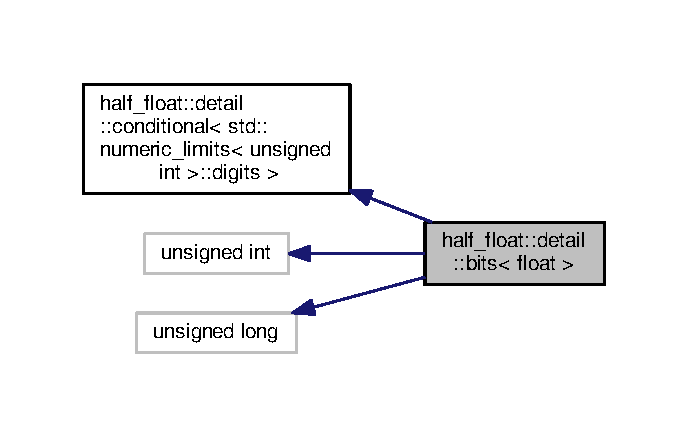
\includegraphics[width=330pt]{structhalf__float_1_1detail_1_1bits_3_01float_01_4__inherit__graph}
\end{center}
\end{figure}


Collaboration diagram for half\+\_\+float\+:\+:detail\+:\+:bits$<$ float $>$\+:
\nopagebreak
\begin{figure}[H]
\begin{center}
\leavevmode
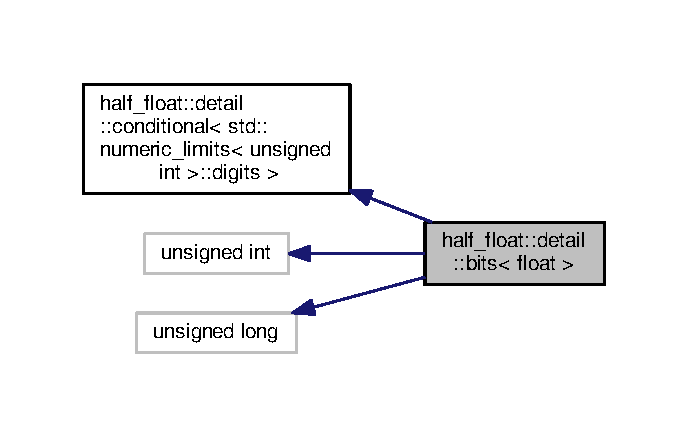
\includegraphics[width=330pt]{structhalf__float_1_1detail_1_1bits_3_01float_01_4__coll__graph}
\end{center}
\end{figure}
\subsection*{Additional Inherited Members}


\subsection{Detailed Description}
\subsubsection*{template$<$$>$\\*
struct half\+\_\+float\+::detail\+::bits$<$ float $>$}

Unsigned integer of (at least) 32 bits width. 

The documentation for this struct was generated from the following file\+:\begin{DoxyCompactItemize}
\item 
/home/rfmeas/project/gxx/gxx/math/\hyperlink{half_8h}{half.\+h}\end{DoxyCompactItemize}

\hypertarget{structhalf__float_1_1detail_1_1bits_3_01volatile_01T_01_4}{}\section{half\+\_\+float\+:\+:detail\+:\+:bits$<$ volatile T $>$ Struct Template Reference}
\label{structhalf__float_1_1detail_1_1bits_3_01volatile_01T_01_4}\index{half\+\_\+float\+::detail\+::bits$<$ volatile T $>$@{half\+\_\+float\+::detail\+::bits$<$ volatile T $>$}}


Inheritance diagram for half\+\_\+float\+:\+:detail\+:\+:bits$<$ volatile T $>$\+:
\nopagebreak
\begin{figure}[H]
\begin{center}
\leavevmode
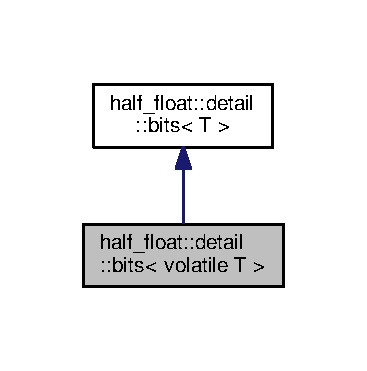
\includegraphics[width=176pt]{structhalf__float_1_1detail_1_1bits_3_01volatile_01T_01_4__inherit__graph}
\end{center}
\end{figure}


Collaboration diagram for half\+\_\+float\+:\+:detail\+:\+:bits$<$ volatile T $>$\+:
\nopagebreak
\begin{figure}[H]
\begin{center}
\leavevmode
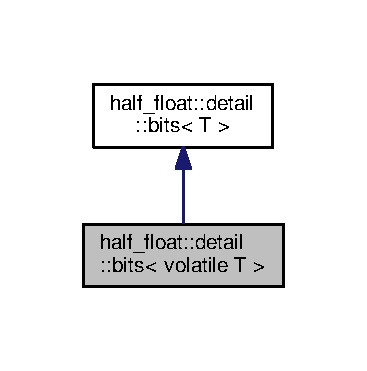
\includegraphics[width=176pt]{structhalf__float_1_1detail_1_1bits_3_01volatile_01T_01_4__coll__graph}
\end{center}
\end{figure}
\subsection*{Additional Inherited Members}


The documentation for this struct was generated from the following file\+:\begin{DoxyCompactItemize}
\item 
/home/rfmeas/project/gxx/gxx/math/\hyperlink{half_8h}{half.\+h}\end{DoxyCompactItemize}

\hypertarget{structhalf__float_1_1detail_1_1bool__type}{}\section{half\+\_\+float\+:\+:detail\+:\+:bool\+\_\+type$<$ bool $>$ Struct Template Reference}
\label{structhalf__float_1_1detail_1_1bool__type}\index{half\+\_\+float\+::detail\+::bool\+\_\+type$<$ bool $>$@{half\+\_\+float\+::detail\+::bool\+\_\+type$<$ bool $>$}}


Helper for tag dispatching.  




{\ttfamily \#include $<$half.\+h$>$}



Inheritance diagram for half\+\_\+float\+:\+:detail\+:\+:bool\+\_\+type$<$ bool $>$\+:
\nopagebreak
\begin{figure}[H]
\begin{center}
\leavevmode
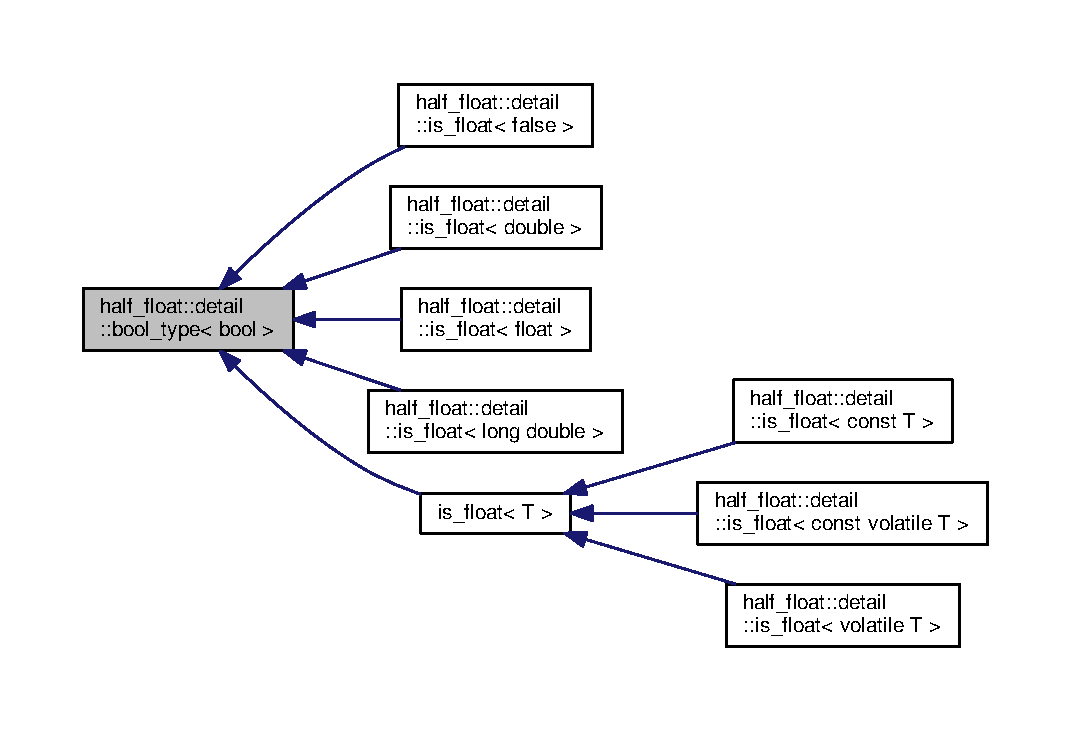
\includegraphics[width=350pt]{structhalf__float_1_1detail_1_1bool__type__inherit__graph}
\end{center}
\end{figure}


\subsection{Detailed Description}
\subsubsection*{template$<$bool$>$\\*
struct half\+\_\+float\+::detail\+::bool\+\_\+type$<$ bool $>$}

Helper for tag dispatching. 

The documentation for this struct was generated from the following file\+:\begin{DoxyCompactItemize}
\item 
/home/rfmeas/project/gxx/gxx/math/\hyperlink{half_8h}{half.\+h}\end{DoxyCompactItemize}

\hypertarget{structgxx_1_1geom2_1_1boundbox}{}\section{gxx\+:\+:geom2\+:\+:boundbox Struct Reference}
\label{structgxx_1_1geom2_1_1boundbox}\index{gxx\+::geom2\+::boundbox@{gxx\+::geom2\+::boundbox}}


Collaboration diagram for gxx\+:\+:geom2\+:\+:boundbox\+:
\nopagebreak
\begin{figure}[H]
\begin{center}
\leavevmode
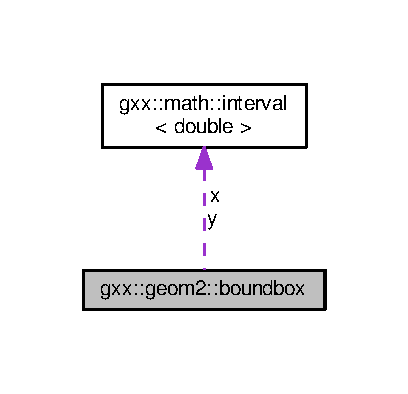
\includegraphics[width=196pt]{structgxx_1_1geom2_1_1boundbox__coll__graph}
\end{center}
\end{figure}
\subsection*{Public Member Functions}
\begin{DoxyCompactItemize}
\item 
{\bfseries boundbox} (double x1, double x2, double y1, double y2)\hypertarget{structgxx_1_1geom2_1_1boundbox_a557ce252a0c79cd3fcdd6bfdc8083eb6}{}\label{structgxx_1_1geom2_1_1boundbox_a557ce252a0c79cd3fcdd6bfdc8083eb6}

\item 
bool {\bfseries can\+\_\+intersect} (const \hyperlink{structgxx_1_1geom2_1_1boundbox}{boundbox} \&oth) const \hypertarget{structgxx_1_1geom2_1_1boundbox_a89aa04b662e689b2ca5c1ebbeb4267ac}{}\label{structgxx_1_1geom2_1_1boundbox_a89aa04b662e689b2ca5c1ebbeb4267ac}

\end{DoxyCompactItemize}
\subsection*{Public Attributes}
\begin{DoxyCompactItemize}
\item 
\hyperlink{classgxx_1_1math_1_1interval}{gxx\+::math\+::interval}$<$ double $>$ {\bfseries x}\hypertarget{structgxx_1_1geom2_1_1boundbox_ae431a779a4fd01ea6f154287b242e01c}{}\label{structgxx_1_1geom2_1_1boundbox_ae431a779a4fd01ea6f154287b242e01c}

\item 
\hyperlink{classgxx_1_1math_1_1interval}{gxx\+::math\+::interval}$<$ double $>$ {\bfseries y}\hypertarget{structgxx_1_1geom2_1_1boundbox_a260fb71bc68508e5148b32b196e656dc}{}\label{structgxx_1_1geom2_1_1boundbox_a260fb71bc68508e5148b32b196e656dc}

\end{DoxyCompactItemize}


The documentation for this struct was generated from the following file\+:\begin{DoxyCompactItemize}
\item 
/home/rfmeas/project/gxx/gxx/geom/geom2.\+h\end{DoxyCompactItemize}

\hypertarget{classgxx_1_1ngeom_1_1bounded__curve}{}\section{gxx\+:\+:ngeom\+:\+:bounded\+\_\+curve Class Reference}
\label{classgxx_1_1ngeom_1_1bounded__curve}\index{gxx\+::ngeom\+::bounded\+\_\+curve@{gxx\+::ngeom\+::bounded\+\_\+curve}}


Inheritance diagram for gxx\+:\+:ngeom\+:\+:bounded\+\_\+curve\+:
% FIG 0


Collaboration diagram for gxx\+:\+:ngeom\+:\+:bounded\+\_\+curve\+:
% FIG 1
\subsection*{Public Member Functions}
\begin{DoxyCompactItemize}
\item 
{\bfseries bounded\+\_\+curve} (double tmin, double tmax)\hypertarget{classgxx_1_1ngeom_1_1bounded__curve_a84ea6de9c1c738bad9192193b7819861}{}\label{classgxx_1_1ngeom_1_1bounded__curve_a84ea6de9c1c738bad9192193b7819861}

\end{DoxyCompactItemize}
\subsection*{Public Attributes}
\begin{DoxyCompactItemize}
\item 
double {\bfseries tmin}\hypertarget{classgxx_1_1ngeom_1_1bounded__curve_aba2a3d39bcd4779265f6fca5a2e51643}{}\label{classgxx_1_1ngeom_1_1bounded__curve_aba2a3d39bcd4779265f6fca5a2e51643}

\item 
double {\bfseries tmax}\hypertarget{classgxx_1_1ngeom_1_1bounded__curve_a2708098aec43031f7c4e697c9fba3e76}{}\label{classgxx_1_1ngeom_1_1bounded__curve_a2708098aec43031f7c4e697c9fba3e76}

\end{DoxyCompactItemize}


The documentation for this class was generated from the following file\+:\begin{DoxyCompactItemize}
\item 
/home/rfmeas/project/gxx/gxx/geom/ncurve.\+h\end{DoxyCompactItemize}

\hypertarget{classgxx_1_1buffer}{}\section{gxx\+:\+:buffer Class Reference}
\label{classgxx_1_1buffer}\index{gxx\+::buffer@{gxx\+::buffer}}


Inheritance diagram for gxx\+:\+:buffer\+:
% FIG 0
\subsection*{Public Member Functions}
\begin{DoxyCompactItemize}
\item 
{\bfseries buffer} (const void $\ast$\+\_\+buf, size\+\_\+t \+\_\+sz)\hypertarget{classgxx_1_1buffer_ab50e6857985ce25bc482ac4a915adf54}{}\label{classgxx_1_1buffer_ab50e6857985ce25bc482ac4a915adf54}

\item 
{\footnotesize template$<$size\+\_\+t N$>$ }\\{\bfseries buffer} (const char(\&arr)\mbox{[}N\mbox{]})\hypertarget{classgxx_1_1buffer_ade202d73586e409e1ab396c87122eeba}{}\label{classgxx_1_1buffer_ade202d73586e409e1ab396c87122eeba}

\item 
bool {\bfseries operator==} (const \hyperlink{classgxx_1_1buffer}{buffer} \&other) const \hypertarget{classgxx_1_1buffer_a300eb1e67de3904c7c88535521b8f9b1}{}\label{classgxx_1_1buffer_a300eb1e67de3904c7c88535521b8f9b1}

\item 
bool {\bfseries operator==} (const char $\ast$str)\hypertarget{classgxx_1_1buffer_a49845b11c97de6da87ed93364a07ef7a}{}\label{classgxx_1_1buffer_a49845b11c97de6da87ed93364a07ef7a}

\item 
char {\bfseries operator\mbox{[}$\,$\mbox{]}} (size\+\_\+t num)\hypertarget{classgxx_1_1buffer_a6b7b7877670efae896cbafa492873562}{}\label{classgxx_1_1buffer_a6b7b7877670efae896cbafa492873562}

\item 
{\bfseries A\+C\+C\+E\+S\+S\+OR} (data, buf)\hypertarget{classgxx_1_1buffer_a9beea8552a484e2605ce1fb94795fcf2}{}\label{classgxx_1_1buffer_a9beea8552a484e2605ce1fb94795fcf2}

\item 
{\bfseries A\+C\+C\+E\+S\+S\+OR} (size, sz)\hypertarget{classgxx_1_1buffer_a0ff37a6b6eab992deaaaf1a4e14bdc90}{}\label{classgxx_1_1buffer_a0ff37a6b6eab992deaaaf1a4e14bdc90}

\item 
char $\ast$ {\bfseries begin} ()\hypertarget{classgxx_1_1buffer_a2e2a945c167dc857f33b57ce676219ee}{}\label{classgxx_1_1buffer_a2e2a945c167dc857f33b57ce676219ee}

\item 
char $\ast$ {\bfseries end} ()\hypertarget{classgxx_1_1buffer_a5b4f116f5dacf672b98614a609fc6302}{}\label{classgxx_1_1buffer_a5b4f116f5dacf672b98614a609fc6302}

\item 
bool {\bfseries empty} ()\hypertarget{classgxx_1_1buffer_a9aaf7c7f29e6a870cde109ca7a02623f}{}\label{classgxx_1_1buffer_a9aaf7c7f29e6a870cde109ca7a02623f}

\item 
\hyperlink{classgxx_1_1buffer}{buffer} {\bfseries slice} (size\+\_\+t idx, size\+\_\+t \+\_\+sz)\hypertarget{classgxx_1_1buffer_aae963da3cb2afe7189638ae39fca540d}{}\label{classgxx_1_1buffer_aae963da3cb2afe7189638ae39fca540d}

\end{DoxyCompactItemize}
\subsection*{Static Public Member Functions}
\begin{DoxyCompactItemize}
\item 
static \hyperlink{classgxx_1_1buffer}{gxx\+::buffer} {\bfseries from\+\_\+string} (const std\+::string \&str)\hypertarget{classgxx_1_1buffer_ad66a56c6f559991a66b4fd88bad79f63}{}\label{classgxx_1_1buffer_ad66a56c6f559991a66b4fd88bad79f63}

\item 
static \hyperlink{classgxx_1_1buffer}{gxx\+::buffer} {\bfseries on\+\_\+string} (const std\+::string \&str)\hypertarget{classgxx_1_1buffer_a9606de5a1ece5a0d81d5c47a99cdf68d}{}\label{classgxx_1_1buffer_a9606de5a1ece5a0d81d5c47a99cdf68d}

\item 
{\footnotesize template$<$typename T $>$ }\\static \hyperlink{classgxx_1_1buffer}{gxx\+::buffer} {\bfseries on\+\_\+object} (T \&obj)\hypertarget{classgxx_1_1buffer_a96279b8e4c96eb322d7bb589fe6f7932}{}\label{classgxx_1_1buffer_a96279b8e4c96eb322d7bb589fe6f7932}

\end{DoxyCompactItemize}
\subsection*{Protected Attributes}
\begin{DoxyCompactItemize}
\item 
char $\ast$ {\bfseries buf}\hypertarget{classgxx_1_1buffer_a8fdf505343749bc0c21536b6fb00ece8}{}\label{classgxx_1_1buffer_a8fdf505343749bc0c21536b6fb00ece8}

\item 
size\+\_\+t {\bfseries sz}\hypertarget{classgxx_1_1buffer_a52bbe79e6c889e3444bb9c4c2b653f0d}{}\label{classgxx_1_1buffer_a52bbe79e6c889e3444bb9c4c2b653f0d}

\end{DoxyCompactItemize}


The documentation for this class was generated from the following file\+:\begin{DoxyCompactItemize}
\item 
/home/rfmeas/project/gxx/gxx/buffer.\+h\end{DoxyCompactItemize}

\hypertarget{classgxx_1_1io_1_1bufreader}{}\section{gxx\+:\+:io\+:\+:bufreader Class Reference}
\label{classgxx_1_1io_1_1bufreader}\index{gxx\+::io\+::bufreader@{gxx\+::io\+::bufreader}}


Inheritance diagram for gxx\+:\+:io\+:\+:bufreader\+:
\nopagebreak
\begin{figure}[H]
\begin{center}
\leavevmode
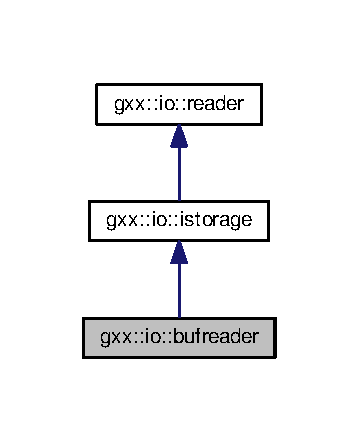
\includegraphics[width=172pt]{classgxx_1_1io_1_1bufreader__inherit__graph}
\end{center}
\end{figure}


Collaboration diagram for gxx\+:\+:io\+:\+:bufreader\+:
\nopagebreak
\begin{figure}[H]
\begin{center}
\leavevmode
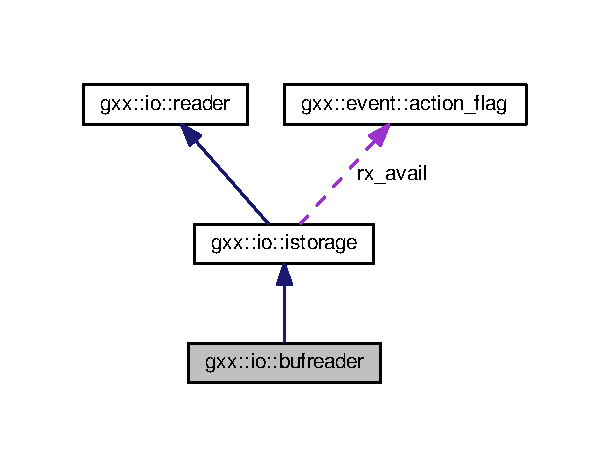
\includegraphics[width=293pt]{classgxx_1_1io_1_1bufreader__coll__graph}
\end{center}
\end{figure}
\subsection*{Public Member Functions}
\begin{DoxyCompactItemize}
\item 
{\bfseries bufreader} (\hyperlink{classgxx_1_1buffer}{gxx\+::buffer} buf)\hypertarget{classgxx_1_1io_1_1bufreader_a871b9310e3a430f104db147871fb93fa}{}\label{classgxx_1_1io_1_1bufreader_a871b9310e3a430f104db147871fb93fa}

\item 
int {\bfseries avail} ()\hypertarget{classgxx_1_1io_1_1bufreader_a49b787c9b5416fe85e7307015d8839e5}{}\label{classgxx_1_1io_1_1bufreader_a49b787c9b5416fe85e7307015d8839e5}

\item 
int {\bfseries read\+Data} (char $\ast$dat, size\+\_\+t sz) override\hypertarget{classgxx_1_1io_1_1bufreader_aa329e29d43c25d0565c56f727ca97ea0}{}\label{classgxx_1_1io_1_1bufreader_aa329e29d43c25d0565c56f727ca97ea0}

\end{DoxyCompactItemize}
\subsection*{Additional Inherited Members}


The documentation for this class was generated from the following file\+:\begin{DoxyCompactItemize}
\item 
/home/rfmeas/project/gxx/gxx/io/bufreader.\+h\end{DoxyCompactItemize}

\hypertarget{classgxx_1_1io_1_1bufwriter}{}\section{gxx\+:\+:io\+:\+:bufwriter Class Reference}
\label{classgxx_1_1io_1_1bufwriter}\index{gxx\+::io\+::bufwriter@{gxx\+::io\+::bufwriter}}


Inheritance diagram for gxx\+:\+:io\+:\+:bufwriter\+:
\nopagebreak
\begin{figure}[H]
\begin{center}
\leavevmode
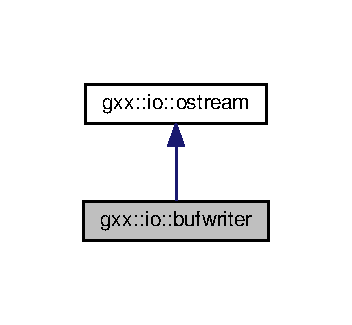
\includegraphics[width=169pt]{classgxx_1_1io_1_1bufwriter__inherit__graph}
\end{center}
\end{figure}


Collaboration diagram for gxx\+:\+:io\+:\+:bufwriter\+:
\nopagebreak
\begin{figure}[H]
\begin{center}
\leavevmode
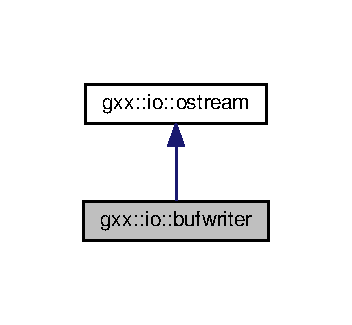
\includegraphics[width=169pt]{classgxx_1_1io_1_1bufwriter__coll__graph}
\end{center}
\end{figure}
\subsection*{Public Member Functions}
\begin{DoxyCompactItemize}
\item 
{\bfseries bufwriter} (\hyperlink{classgxx_1_1buffer}{gxx\+::buffer} buf)\hypertarget{classgxx_1_1io_1_1bufwriter_a5b300f0fd662417ebbbac62e948437ce}{}\label{classgxx_1_1io_1_1bufwriter_a5b300f0fd662417ebbbac62e948437ce}

\item 
int {\bfseries write\+Data} (const char $\ast$str, size\+\_\+t sz)\hypertarget{classgxx_1_1io_1_1bufwriter_aad34a02b76fbc5f6abfad4f59bc76262}{}\label{classgxx_1_1io_1_1bufwriter_aad34a02b76fbc5f6abfad4f59bc76262}

\item 
size\+\_\+t {\bfseries size} ()\hypertarget{classgxx_1_1io_1_1bufwriter_aee941af370762885650fb7a07fe5ab20}{}\label{classgxx_1_1io_1_1bufwriter_aee941af370762885650fb7a07fe5ab20}

\end{DoxyCompactItemize}
\subsection*{Public Attributes}
\begin{DoxyCompactItemize}
\item 
size\+\_\+t {\bfseries cursize} = 0\hypertarget{classgxx_1_1io_1_1bufwriter_af587a495c8a8cf990589469d93fbd0bb}{}\label{classgxx_1_1io_1_1bufwriter_af587a495c8a8cf990589469d93fbd0bb}

\end{DoxyCompactItemize}
\subsection*{Additional Inherited Members}


The documentation for this class was generated from the following file\+:\begin{DoxyCompactItemize}
\item 
/home/rfmeas/project/gxx/gxx/io/bufwriter.\+h\end{DoxyCompactItemize}

\hypertarget{classgxx_1_1bytearray}{}\section{gxx\+:\+:bytearray Class Reference}
\label{classgxx_1_1bytearray}\index{gxx\+::bytearray@{gxx\+::bytearray}}


Inheritance diagram for gxx\+:\+:bytearray\+:
% FIG 0


Collaboration diagram for gxx\+:\+:bytearray\+:
% FIG 1
\subsection*{Public Member Functions}
\begin{DoxyCompactItemize}
\item 
{\bfseries bytearray} (const char $\ast$data, size\+\_\+t sz)\hypertarget{classgxx_1_1bytearray_afcff02af3b1692e16a6db49d9303329e}{}\label{classgxx_1_1bytearray_afcff02af3b1692e16a6db49d9303329e}

\end{DoxyCompactItemize}
\subsection*{Additional Inherited Members}


The documentation for this class was generated from the following file\+:\begin{DoxyCompactItemize}
\item 
/home/rfmeas/project/gxx/gxx/\+H\+I\+D\+E/bytearray.\+h\end{DoxyCompactItemize}

\hypertarget{classgxx_1_1bytering}{}\section{gxx\+:\+:bytering Class Reference}
\label{classgxx_1_1bytering}\index{gxx\+::bytering@{gxx\+::bytering}}
\subsection*{Public Member Functions}
\begin{DoxyCompactItemize}
\item 
{\bfseries bytering} (char $\ast$buf, size\+\_\+t sz)\hypertarget{classgxx_1_1bytering_ae2d328873fd5b03e67383a709bd90826}{}\label{classgxx_1_1bytering_ae2d328873fd5b03e67383a709bd90826}

\item 
{\bfseries bytering} (\hyperlink{classgxx_1_1buffer}{gxx\+::buffer} buf)\hypertarget{classgxx_1_1bytering_a9b8f2cd2c64128653bc8cb96a47c2675}{}\label{classgxx_1_1bytering_a9b8f2cd2c64128653bc8cb96a47c2675}

\item 
void {\bfseries init} (char $\ast$\hyperlink{classgxx_1_1buffer}{buffer}, size\+\_\+t size)\hypertarget{classgxx_1_1bytering_a866ec4e1db4752491af2aaf13ca1271e}{}\label{classgxx_1_1bytering_a866ec4e1db4752491af2aaf13ca1271e}

\item 
bool {\bfseries empty} () volatile\hypertarget{classgxx_1_1bytering_abd8db2cbab231645867d7d4f2b482cf4}{}\label{classgxx_1_1bytering_abd8db2cbab231645867d7d4f2b482cf4}

\item 
int {\bfseries clean} ()\hypertarget{classgxx_1_1bytering_aadcd015c33db152a0539bbc3566474c3}{}\label{classgxx_1_1bytering_aadcd015c33db152a0539bbc3566474c3}

\item 
bool {\bfseries full} ()\hypertarget{classgxx_1_1bytering_a9c038d51bc47c1f9f1158520ac09af7a}{}\label{classgxx_1_1bytering_a9c038d51bc47c1f9f1158520ac09af7a}

\item 
int {\bfseries push} (char c)\hypertarget{classgxx_1_1bytering_ab08e8df59c29e18ee3d2b219697d275e}{}\label{classgxx_1_1bytering_ab08e8df59c29e18ee3d2b219697d275e}

\item 
int {\bfseries push} (const char $\ast$data, size\+\_\+t size)\hypertarget{classgxx_1_1bytering_a0bd8517d3572d3ee95b66abfa3599384}{}\label{classgxx_1_1bytering_a0bd8517d3572d3ee95b66abfa3599384}

\item 
int {\bfseries pop} ()\hypertarget{classgxx_1_1bytering_a797d035bdac1086197108e8c67dc6396}{}\label{classgxx_1_1bytering_a797d035bdac1086197108e8c67dc6396}

\item 
int {\bfseries popn} (char $\ast$data, size\+\_\+t size)\hypertarget{classgxx_1_1bytering_a72f09545c85812a2ab322b3355b4512c}{}\label{classgxx_1_1bytering_a72f09545c85812a2ab322b3355b4512c}

\item 
int {\bfseries pick} ()\hypertarget{classgxx_1_1bytering_ae6fecd2e6f165b489784ce54563af1af}{}\label{classgxx_1_1bytering_ae6fecd2e6f165b489784ce54563af1af}

\item 
int {\bfseries pickn} (char $\ast$data, size\+\_\+t size)\hypertarget{classgxx_1_1bytering_ac14bc1eefb3a9629dcb3df921bc24c2c}{}\label{classgxx_1_1bytering_ac14bc1eefb3a9629dcb3df921bc24c2c}

\item 
\hyperlink{classgxx_1_1buffer}{gxx\+::buffer} {\bfseries first\+\_\+part\+\_\+as\+\_\+buffer} ()\hypertarget{classgxx_1_1bytering_a90fe6c750f2ec2da689bb03052c523fb}{}\label{classgxx_1_1bytering_a90fe6c750f2ec2da689bb03052c523fb}

\item 
\hyperlink{classgxx_1_1buffer}{gxx\+::buffer} {\bfseries last\+\_\+part\+\_\+as\+\_\+buffer} ()\hypertarget{classgxx_1_1bytering_a2270a2ee1053783813b5f4474f9995eb}{}\label{classgxx_1_1bytering_a2270a2ee1053783813b5f4474f9995eb}

\item 
size\+\_\+t {\bfseries avail} ()\hypertarget{classgxx_1_1bytering_ade367bb8d78bee5e4da5474128ccfda3}{}\label{classgxx_1_1bytering_ade367bb8d78bee5e4da5474128ccfda3}

\item 
size\+\_\+t {\bfseries room} ()\hypertarget{classgxx_1_1bytering_a4dd47cc8ea6425f25dab7a2afbdcf682}{}\label{classgxx_1_1bytering_a4dd47cc8ea6425f25dab7a2afbdcf682}

\end{DoxyCompactItemize}


The documentation for this class was generated from the following file\+:\begin{DoxyCompactItemize}
\item 
/home/rfmeas/project/gxx/gxx/bytering.\+h\end{DoxyCompactItemize}

\hypertarget{classgxx_1_1callback}{}\section{gxx\+:\+:callback$<$ R, Args $>$ Class Template Reference}
\label{classgxx_1_1callback}\index{gxx\+::callback$<$ R, Args $>$@{gxx\+::callback$<$ R, Args $>$}}


The documentation for this class was generated from the following file\+:\begin{DoxyCompactItemize}
\item 
/home/rfmeas/project/gxx/gxx/event/delegate.\+h\end{DoxyCompactItemize}

\hypertarget{structgxx_1_1change__basic}{}\section{gxx\+:\+:change\+\_\+basic$<$ T, B $>$ Struct Template Reference}
\label{structgxx_1_1change__basic}\index{gxx\+::change\+\_\+basic$<$ T, B $>$@{gxx\+::change\+\_\+basic$<$ T, B $>$}}


The documentation for this struct was generated from the following file\+:\begin{DoxyCompactItemize}
\item 
/home/rfmeas/project/gxx/gxx/event/delegate.\+h\end{DoxyCompactItemize}

\hypertarget{structgxx_1_1change__basic_3_01T_00_01R_07B_1_1_5_08_07V_8_8_8_08_4}{}\section{gxx\+:\+:change\+\_\+basic$<$ T, R(B\+:\+:$\ast$)(V...)$>$ Struct Template Reference}
\label{structgxx_1_1change__basic_3_01T_00_01R_07B_1_1_5_08_07V_8_8_8_08_4}\index{gxx\+::change\+\_\+basic$<$ T, R(\+B\+::$\ast$)(\+V...)$>$@{gxx\+::change\+\_\+basic$<$ T, R(\+B\+::$\ast$)(\+V...)$>$}}
\subsection*{Public Types}
\begin{DoxyCompactItemize}
\item 
using {\bfseries type} = R(T\+::$\ast$)(V...)\hypertarget{structgxx_1_1change__basic_3_01T_00_01R_07B_1_1_5_08_07V_8_8_8_08_4_a04925e59d8f5baca4577299a5f9e81d0}{}\label{structgxx_1_1change__basic_3_01T_00_01R_07B_1_1_5_08_07V_8_8_8_08_4_a04925e59d8f5baca4577299a5f9e81d0}

\end{DoxyCompactItemize}


The documentation for this struct was generated from the following file\+:\begin{DoxyCompactItemize}
\item 
/home/rfmeas/project/gxx/gxx/event/delegate.\+h\end{DoxyCompactItemize}

\hypertarget{structgxx_1_1chars__set__checker}{}\section{gxx\+:\+:chars\+\_\+set\+\_\+checker Struct Reference}
\label{structgxx_1_1chars__set__checker}\index{gxx\+::chars\+\_\+set\+\_\+checker@{gxx\+::chars\+\_\+set\+\_\+checker}}


Collaboration diagram for gxx\+:\+:chars\+\_\+set\+\_\+checker\+:\nopagebreak
\begin{figure}[H]
\begin{center}
\leavevmode
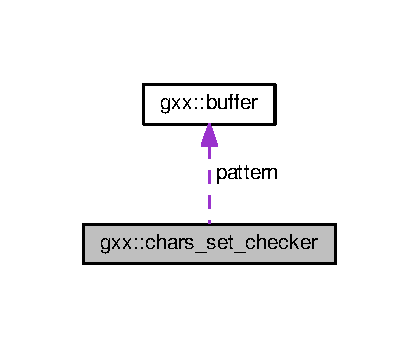
\includegraphics[width=201pt]{structgxx_1_1chars__set__checker__coll__graph}
\end{center}
\end{figure}
\subsection*{Public Member Functions}
\begin{DoxyCompactItemize}
\item 
{\bfseries chars\+\_\+set\+\_\+checker} (\hyperlink{classgxx_1_1buffer}{gxx\+::buffer} \+\_\+pattern, bool \+\_\+tgt=true)\hypertarget{structgxx_1_1chars__set__checker_aa1417ce025b8d17d48fd28fac2fb6f64}{}\label{structgxx_1_1chars__set__checker_aa1417ce025b8d17d48fd28fac2fb6f64}

\item 
bool {\bfseries operator()} (char c)\hypertarget{structgxx_1_1chars__set__checker_a5947c8b51919817e40adf25f93623923}{}\label{structgxx_1_1chars__set__checker_a5947c8b51919817e40adf25f93623923}

\end{DoxyCompactItemize}
\subsection*{Public Attributes}
\begin{DoxyCompactItemize}
\item 
\hyperlink{classgxx_1_1buffer}{gxx\+::buffer} {\bfseries pattern}\hypertarget{structgxx_1_1chars__set__checker_af000461ade68f18a441258d4c08713cb}{}\label{structgxx_1_1chars__set__checker_af000461ade68f18a441258d4c08713cb}

\item 
bool {\bfseries tgt}\hypertarget{structgxx_1_1chars__set__checker_a475f177962094025b8c58022d2635382}{}\label{structgxx_1_1chars__set__checker_a475f177962094025b8c58022d2635382}

\end{DoxyCompactItemize}


The documentation for this struct was generated from the following file\+:\begin{DoxyCompactItemize}
\item 
/home/rfmeas/project/gxx/gxx/creader.\+h\end{DoxyCompactItemize}

\hypertarget{classgxx_1_1CharStrSpec}{}\section{gxx\+:\+:Char\+Str\+Spec Class Reference}
\label{classgxx_1_1CharStrSpec}\index{gxx\+::\+Char\+Str\+Spec@{gxx\+::\+Char\+Str\+Spec}}


Inheritance diagram for gxx\+:\+:Char\+Str\+Spec\+:
\nopagebreak
\begin{figure}[H]
\begin{center}
\leavevmode
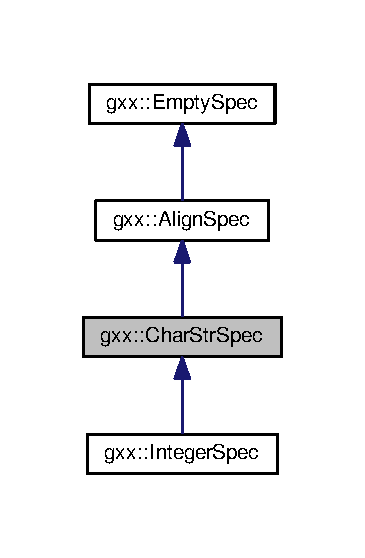
\includegraphics[width=175pt]{classgxx_1_1CharStrSpec__inherit__graph}
\end{center}
\end{figure}


Collaboration diagram for gxx\+:\+:Char\+Str\+Spec\+:
\nopagebreak
\begin{figure}[H]
\begin{center}
\leavevmode
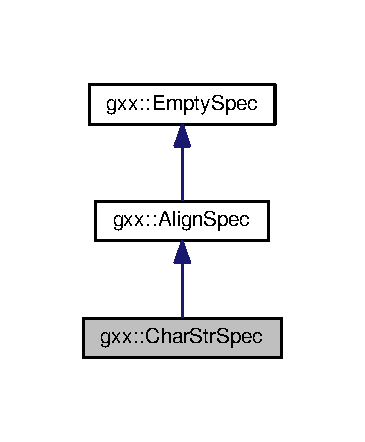
\includegraphics[width=175pt]{classgxx_1_1CharStrSpec__coll__graph}
\end{center}
\end{figure}
\subsection*{Public Member Functions}
\begin{DoxyCompactItemize}
\item 
Char\+Case {\bfseries char\+Case} () const \hypertarget{classgxx_1_1CharStrSpec_a1dc341eb44cbe131c1359d8250db5b22}{}\label{classgxx_1_1CharStrSpec_a1dc341eb44cbe131c1359d8250db5b22}

\item 
\hyperlink{classgxx_1_1CharStrSpec}{Char\+Str\+Spec} \& {\bfseries char\+Case} (Char\+Case ccase)\hypertarget{classgxx_1_1CharStrSpec_a20049f3f82f482bb85160a6d1158714d}{}\label{classgxx_1_1CharStrSpec_a20049f3f82f482bb85160a6d1158714d}

\item 
\hyperlink{classgxx_1_1CharStrSpec}{Char\+Str\+Spec} \& {\bfseries align} (Alignment align)\hypertarget{classgxx_1_1CharStrSpec_a99e021803ace781163acad2b6bd9efd5}{}\label{classgxx_1_1CharStrSpec_a99e021803ace781163acad2b6bd9efd5}

\item 
\hyperlink{classgxx_1_1CharStrSpec}{Char\+Str\+Spec} \& {\bfseries fill} (char fill)\hypertarget{classgxx_1_1CharStrSpec_af6ded10729691615ca0f869af442e1d4}{}\label{classgxx_1_1CharStrSpec_af6ded10729691615ca0f869af442e1d4}

\item 
\hyperlink{classgxx_1_1CharStrSpec}{Char\+Str\+Spec} \& {\bfseries width} (size\+\_\+t width)\hypertarget{classgxx_1_1CharStrSpec_ab53ac51ccdba3528c7d7ac1872974011}{}\label{classgxx_1_1CharStrSpec_ab53ac51ccdba3528c7d7ac1872974011}

\end{DoxyCompactItemize}
\subsection*{Protected Attributes}
\begin{DoxyCompactItemize}
\item 
Char\+Case {\bfseries \+\_\+ccase} = Char\+Case\+::\+Default\hypertarget{classgxx_1_1CharStrSpec_a1dc900c599fa48930a12eade5984c182}{}\label{classgxx_1_1CharStrSpec_a1dc900c599fa48930a12eade5984c182}

\end{DoxyCompactItemize}


The documentation for this class was generated from the following file\+:\begin{DoxyCompactItemize}
\item 
/home/rfmeas/project/gxx/gxx/\+H\+I\+D\+E/io/text\+\_\+writer.\+h\end{DoxyCompactItemize}

\hypertarget{classgxx_1_1io_1_1CharStrSpec}{}\section{gxx\+:\+:io\+:\+:Char\+Str\+Spec Class Reference}
\label{classgxx_1_1io_1_1CharStrSpec}\index{gxx\+::io\+::\+Char\+Str\+Spec@{gxx\+::io\+::\+Char\+Str\+Spec}}


Inheritance diagram for gxx\+:\+:io\+:\+:Char\+Str\+Spec\+:
% FIG 0


Collaboration diagram for gxx\+:\+:io\+:\+:Char\+Str\+Spec\+:
% FIG 1
\subsection*{Public Member Functions}
\begin{DoxyCompactItemize}
\item 
Char\+Case {\bfseries char\+Case} () const \hypertarget{classgxx_1_1io_1_1CharStrSpec_ab3b9dbaf9f770d9a154c6ec8a2594cfb}{}\label{classgxx_1_1io_1_1CharStrSpec_ab3b9dbaf9f770d9a154c6ec8a2594cfb}

\item 
\hyperlink{classgxx_1_1io_1_1CharStrSpec}{Char\+Str\+Spec} \& {\bfseries char\+Case} (Char\+Case ccase)\hypertarget{classgxx_1_1io_1_1CharStrSpec_a7ae04a1d41418f5a856bf5101b27f108}{}\label{classgxx_1_1io_1_1CharStrSpec_a7ae04a1d41418f5a856bf5101b27f108}

\item 
\hyperlink{classgxx_1_1io_1_1CharStrSpec}{Char\+Str\+Spec} \& {\bfseries align} (Alignment align)\hypertarget{classgxx_1_1io_1_1CharStrSpec_ab1c6966b305170da20e3742c64417cce}{}\label{classgxx_1_1io_1_1CharStrSpec_ab1c6966b305170da20e3742c64417cce}

\item 
\hyperlink{classgxx_1_1io_1_1CharStrSpec}{Char\+Str\+Spec} \& {\bfseries fill} (char fill)\hypertarget{classgxx_1_1io_1_1CharStrSpec_af54cb7ea3744f0551d59ae3b91c3969c}{}\label{classgxx_1_1io_1_1CharStrSpec_af54cb7ea3744f0551d59ae3b91c3969c}

\item 
\hyperlink{classgxx_1_1io_1_1CharStrSpec}{Char\+Str\+Spec} \& {\bfseries width} (size\+\_\+t width)\hypertarget{classgxx_1_1io_1_1CharStrSpec_a49603cb128afc1799f20fa7882e79f55}{}\label{classgxx_1_1io_1_1CharStrSpec_a49603cb128afc1799f20fa7882e79f55}

\item 
Char\+Case {\bfseries char\+Case} () const \hypertarget{classgxx_1_1io_1_1CharStrSpec_ab3b9dbaf9f770d9a154c6ec8a2594cfb}{}\label{classgxx_1_1io_1_1CharStrSpec_ab3b9dbaf9f770d9a154c6ec8a2594cfb}

\item 
\hyperlink{classgxx_1_1io_1_1CharStrSpec}{Char\+Str\+Spec} \& {\bfseries char\+Case} (Char\+Case ccase)\hypertarget{classgxx_1_1io_1_1CharStrSpec_a7ae04a1d41418f5a856bf5101b27f108}{}\label{classgxx_1_1io_1_1CharStrSpec_a7ae04a1d41418f5a856bf5101b27f108}

\item 
\hyperlink{classgxx_1_1io_1_1CharStrSpec}{Char\+Str\+Spec} \& {\bfseries align} (Alignment align)\hypertarget{classgxx_1_1io_1_1CharStrSpec_ab1c6966b305170da20e3742c64417cce}{}\label{classgxx_1_1io_1_1CharStrSpec_ab1c6966b305170da20e3742c64417cce}

\item 
\hyperlink{classgxx_1_1io_1_1CharStrSpec}{Char\+Str\+Spec} \& {\bfseries fill} (char fill)\hypertarget{classgxx_1_1io_1_1CharStrSpec_af54cb7ea3744f0551d59ae3b91c3969c}{}\label{classgxx_1_1io_1_1CharStrSpec_af54cb7ea3744f0551d59ae3b91c3969c}

\item 
\hyperlink{classgxx_1_1io_1_1CharStrSpec}{Char\+Str\+Spec} \& {\bfseries width} (size\+\_\+t width)\hypertarget{classgxx_1_1io_1_1CharStrSpec_a49603cb128afc1799f20fa7882e79f55}{}\label{classgxx_1_1io_1_1CharStrSpec_a49603cb128afc1799f20fa7882e79f55}

\item 
Char\+Case {\bfseries char\+Case} () const \hypertarget{classgxx_1_1io_1_1CharStrSpec_ab3b9dbaf9f770d9a154c6ec8a2594cfb}{}\label{classgxx_1_1io_1_1CharStrSpec_ab3b9dbaf9f770d9a154c6ec8a2594cfb}

\item 
\hyperlink{classgxx_1_1io_1_1CharStrSpec}{Char\+Str\+Spec} \& {\bfseries char\+Case} (Char\+Case ccase)\hypertarget{classgxx_1_1io_1_1CharStrSpec_a7ae04a1d41418f5a856bf5101b27f108}{}\label{classgxx_1_1io_1_1CharStrSpec_a7ae04a1d41418f5a856bf5101b27f108}

\item 
\hyperlink{classgxx_1_1io_1_1CharStrSpec}{Char\+Str\+Spec} \& {\bfseries align} (Alignment align)\hypertarget{classgxx_1_1io_1_1CharStrSpec_ab1c6966b305170da20e3742c64417cce}{}\label{classgxx_1_1io_1_1CharStrSpec_ab1c6966b305170da20e3742c64417cce}

\item 
\hyperlink{classgxx_1_1io_1_1CharStrSpec}{Char\+Str\+Spec} \& {\bfseries fill} (char fill)\hypertarget{classgxx_1_1io_1_1CharStrSpec_af54cb7ea3744f0551d59ae3b91c3969c}{}\label{classgxx_1_1io_1_1CharStrSpec_af54cb7ea3744f0551d59ae3b91c3969c}

\item 
\hyperlink{classgxx_1_1io_1_1CharStrSpec}{Char\+Str\+Spec} \& {\bfseries width} (size\+\_\+t width)\hypertarget{classgxx_1_1io_1_1CharStrSpec_a49603cb128afc1799f20fa7882e79f55}{}\label{classgxx_1_1io_1_1CharStrSpec_a49603cb128afc1799f20fa7882e79f55}

\end{DoxyCompactItemize}
\subsection*{Protected Attributes}
\begin{DoxyCompactItemize}
\item 
Char\+Case {\bfseries \+\_\+ccase} = Char\+Case\+::\+Default\hypertarget{classgxx_1_1io_1_1CharStrSpec_abeda9480c8b16d1c07bce613ca42be1e}{}\label{classgxx_1_1io_1_1CharStrSpec_abeda9480c8b16d1c07bce613ca42be1e}

\end{DoxyCompactItemize}


The documentation for this class was generated from the following file\+:\begin{DoxyCompactItemize}
\item 
/home/rfmeas/project/gxx/gxx/\+H\+I\+D\+E/ionew/format\+\_\+writer.\+h\end{DoxyCompactItemize}

\hypertarget{classgxx_1_1geom2_1_1circle}{}\section{gxx\+:\+:geom2\+:\+:circle Class Reference}
\label{classgxx_1_1geom2_1_1circle}\index{gxx\+::geom2\+::circle@{gxx\+::geom2\+::circle}}


Inheritance diagram for gxx\+:\+:geom2\+:\+:circle\+:
% FIG 0


Collaboration diagram for gxx\+:\+:geom2\+:\+:circle\+:
% FIG 1
\subsection*{Public Member Functions}
\begin{DoxyCompactItemize}
\item 
{\bfseries A\+C\+C\+E\+S\+S\+OR} (center, l)\hypertarget{classgxx_1_1geom2_1_1circle_a3fbb943fcea9df55e691b65dc692180a}{}\label{classgxx_1_1geom2_1_1circle_a3fbb943fcea9df55e691b65dc692180a}

\item 
{\bfseries A\+C\+C\+E\+S\+S\+OR} (radius, r)\hypertarget{classgxx_1_1geom2_1_1circle_abf1e43383d40e0531098a1a9c60620e7}{}\label{classgxx_1_1geom2_1_1circle_abf1e43383d40e0531098a1a9c60620e7}

\item 
{\bfseries circle} (double r, const \hyperlink{classmalgo_1_1vector2}{point} \&l, const \hyperlink{classmalgo_1_1unit__vector2}{direction} \&d=\hyperlink{classmalgo_1_1unit__vector2}{direction}(1, 0, false))\hypertarget{classgxx_1_1geom2_1_1circle_a8ecb3cd0d6a38d9554b9e3bae2ac3392}{}\label{classgxx_1_1geom2_1_1circle_a8ecb3cd0d6a38d9554b9e3bae2ac3392}

\item 
\hyperlink{classmalgo_1_1vector2}{point} {\bfseries d0} (double t) const override\hypertarget{classgxx_1_1geom2_1_1circle_af079d357aa91bb278f3fabf190caa665}{}\label{classgxx_1_1geom2_1_1circle_af079d357aa91bb278f3fabf190caa665}

\item 
\hyperlink{classmalgo_1_1vector2}{vector} {\bfseries d1} (double t) const override\hypertarget{classgxx_1_1geom2_1_1circle_ab4789d64c29578ce2e70a241fabfeee3}{}\label{classgxx_1_1geom2_1_1circle_ab4789d64c29578ce2e70a241fabfeee3}

\item 
double {\bfseries tmax} () override\hypertarget{classgxx_1_1geom2_1_1circle_a97cac06440f256ec67c680fbc973e9e6}{}\label{classgxx_1_1geom2_1_1circle_a97cac06440f256ec67c680fbc973e9e6}

\item 
size\+\_\+t {\bfseries print\+To} (\hyperlink{classgxx_1_1io_1_1ostream}{gxx\+::io\+::ostream} \&o) const override\hypertarget{classgxx_1_1geom2_1_1circle_ab1883e9a35d83218c36b32413c6fb4ac}{}\label{classgxx_1_1geom2_1_1circle_ab1883e9a35d83218c36b32413c6fb4ac}

\item 
double {\bfseries sparam} ()\hypertarget{classgxx_1_1geom2_1_1circle_a26e16cd9190f29df3dcfbbce020defc3}{}\label{classgxx_1_1geom2_1_1circle_a26e16cd9190f29df3dcfbbce020defc3}

\item 
bool {\bfseries is\+\_\+analityc} () override\hypertarget{classgxx_1_1geom2_1_1circle_aa81b4ec51dd1f61a9b7ef39a770257f0}{}\label{classgxx_1_1geom2_1_1circle_aa81b4ec51dd1f61a9b7ef39a770257f0}

\item 
std\+::shared\+\_\+ptr$<$ \hyperlink{classgxx_1_1geom2_1_1curve}{curve} $>$ {\bfseries translate} (double x, double y)\hypertarget{classgxx_1_1geom2_1_1circle_a03b81bb9b51fd768a581833442b57fda}{}\label{classgxx_1_1geom2_1_1circle_a03b81bb9b51fd768a581833442b57fda}

\end{DoxyCompactItemize}
\subsection*{Public Attributes}
\begin{DoxyCompactItemize}
\item 
\hyperlink{classmalgo_1_1vector2}{point} {\bfseries l}\hypertarget{classgxx_1_1geom2_1_1circle_a5f4ba09d4f8981de8a5209d0973d18f8}{}\label{classgxx_1_1geom2_1_1circle_a5f4ba09d4f8981de8a5209d0973d18f8}

\item 
double {\bfseries r}\hypertarget{classgxx_1_1geom2_1_1circle_a38247ff2ad6189df86efd599bc954898}{}\label{classgxx_1_1geom2_1_1circle_a38247ff2ad6189df86efd599bc954898}

\item 
double {\bfseries sp}\hypertarget{classgxx_1_1geom2_1_1circle_a0e1c9475ab3dc37c916ba2af119b4da8}{}\label{classgxx_1_1geom2_1_1circle_a0e1c9475ab3dc37c916ba2af119b4da8}

\item 
\hyperlink{classmalgo_1_1unit__vector2}{direction} {\bfseries dirx}\hypertarget{classgxx_1_1geom2_1_1circle_a8faa950866fa901990f179bfb4544b3f}{}\label{classgxx_1_1geom2_1_1circle_a8faa950866fa901990f179bfb4544b3f}

\end{DoxyCompactItemize}


The documentation for this class was generated from the following file\+:\begin{DoxyCompactItemize}
\item 
/home/rfmeas/project/gxx/gxx/geom/geom2.\+h\end{DoxyCompactItemize}

\hypertarget{structrabbit_1_1circle2}{}\section{rabbit\+:\+:circle2 Struct Reference}
\label{structrabbit_1_1circle2}\index{rabbit\+::circle2@{rabbit\+::circle2}}


Inheritance diagram for rabbit\+:\+:circle2\+:
\nopagebreak
\begin{figure}[H]
\begin{center}
\leavevmode
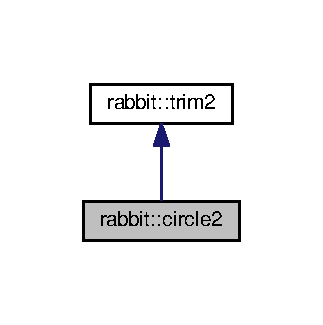
\includegraphics[width=155pt]{structrabbit_1_1circle2__inherit__graph}
\end{center}
\end{figure}


Collaboration diagram for rabbit\+:\+:circle2\+:
\nopagebreak
\begin{figure}[H]
\begin{center}
\leavevmode
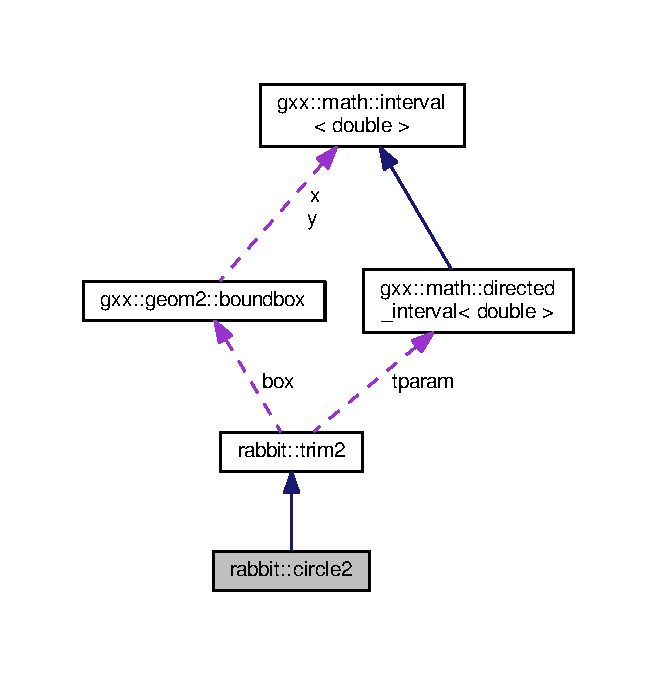
\includegraphics[width=316pt]{structrabbit_1_1circle2__coll__graph}
\end{center}
\end{figure}
\subsection*{Public Member Functions}
\begin{DoxyCompactItemize}
\item 
{\bfseries circle2} (double rad)\hypertarget{structrabbit_1_1circle2_a79dc420bd96a245af5f214d833f50f87}{}\label{structrabbit_1_1circle2_a79dc420bd96a245af5f214d833f50f87}

\end{DoxyCompactItemize}
\subsection*{Additional Inherited Members}


The documentation for this struct was generated from the following file\+:\begin{DoxyCompactItemize}
\item 
/home/rfmeas/project/gxx/gxx/rabbit/topo2.\+h\end{DoxyCompactItemize}

\hypertarget{classgxx_1_1cliopts}{}\section{gxx\+:\+:cliopts Class Reference}
\label{classgxx_1_1cliopts}\index{gxx\+::cliopts@{gxx\+::cliopts}}
\subsection*{Public Types}
\begin{DoxyCompactItemize}
\item 
enum {\bfseries Autom\+State} \{ {\bfseries Wait\+Value}, 
{\bfseries Normal}
 \}\hypertarget{classgxx_1_1cliopts_a3ab2bce5df9288c116ac00d1504cfeea}{}\label{classgxx_1_1cliopts_a3ab2bce5df9288c116ac00d1504cfeea}

\end{DoxyCompactItemize}
\subsection*{Public Member Functions}
\begin{DoxyCompactItemize}
\item 
void {\bfseries add\+\_\+bool} (const char $\ast$l, char s, bool def)\hypertarget{classgxx_1_1cliopts_ae689fa36031b2f658351566aa071db2e}{}\label{classgxx_1_1cliopts_ae689fa36031b2f658351566aa071db2e}

\item 
void {\bfseries add\+\_\+integer} (const char $\ast$l, char s, int32\+\_\+t def)\hypertarget{classgxx_1_1cliopts_a597b367bb723b5e73de4ae2baa469760}{}\label{classgxx_1_1cliopts_a597b367bb723b5e73de4ae2baa469760}

\item 
void {\bfseries add\+\_\+string} (const char $\ast$l, char s, std\+::string def)\hypertarget{classgxx_1_1cliopts_a29ce9b9348072dcd945981cebad8ddc1}{}\label{classgxx_1_1cliopts_a29ce9b9348072dcd945981cebad8ddc1}

\item 
void {\bfseries add\+\_\+string} (const char $\ast$l, char s, const char $\ast$def)\hypertarget{classgxx_1_1cliopts_ae2b28f83c317888494b2819b151d6652}{}\label{classgxx_1_1cliopts_ae2b28f83c317888494b2819b151d6652}

\item 
void {\bfseries add\+\_\+option} (const char $\ast$l, char s)\hypertarget{classgxx_1_1cliopts_a22c702620fe35d24abce9c99d38629c9}{}\label{classgxx_1_1cliopts_a22c702620fe35d24abce9c99d38629c9}

\item 
\hyperlink{classgxx_1_1result__type_1_1result}{result}$<$ opt $\ast$ $>$ {\bfseries get\+\_\+opt} (const char $\ast$l)\hypertarget{classgxx_1_1cliopts_a4479d8c7b3e9bc9a12d2dc1887633f9d}{}\label{classgxx_1_1cliopts_a4479d8c7b3e9bc9a12d2dc1887633f9d}

\item 
\hyperlink{classgxx_1_1result__type_1_1result}{result}$<$ opt $\ast$ $>$ {\bfseries get\+\_\+opt} (char c)\hypertarget{classgxx_1_1cliopts_aa73c0d8d2658e2a4339f5e13f69b9ace}{}\label{classgxx_1_1cliopts_aa73c0d8d2658e2a4339f5e13f69b9ace}

\item 
\hyperlink{classgxx_1_1result__type_1_1result}{result}$<$ opt $\ast$ $>$ {\bfseries get\+\_\+opt} (const char $\ast$l, Type type)\hypertarget{classgxx_1_1cliopts_a77194b27fe885effa4c098ad8cbb8a25}{}\label{classgxx_1_1cliopts_a77194b27fe885effa4c098ad8cbb8a25}

\item 
\hyperlink{classgxx_1_1result__type_1_1result}{result}$<$ std\+::string $>$ {\bfseries get\+\_\+string} (const char $\ast$l)\hypertarget{classgxx_1_1cliopts_a2fcd50f503346b00dbf8b6880d3d3802}{}\label{classgxx_1_1cliopts_a2fcd50f503346b00dbf8b6880d3d3802}

\item 
\hyperlink{classgxx_1_1result__type_1_1result}{result}$<$ int32\+\_\+t $>$ {\bfseries get\+\_\+integer} (const char $\ast$l)\hypertarget{classgxx_1_1cliopts_a69cde10987004349a0c8449bc7edbde8}{}\label{classgxx_1_1cliopts_a69cde10987004349a0c8449bc7edbde8}

\item 
\hyperlink{classgxx_1_1result__type_1_1result}{result}$<$ bool $>$ {\bfseries get\+\_\+bool} (const char $\ast$l)\hypertarget{classgxx_1_1cliopts_a3e1794230a882a3d0ee1eb6750a9fad3}{}\label{classgxx_1_1cliopts_a3e1794230a882a3d0ee1eb6750a9fad3}

\item 
\hyperlink{classgxx_1_1result__type_1_1result}{result}$<$ bool $>$ {\bfseries get\+\_\+option} (const char $\ast$l)\hypertarget{classgxx_1_1cliopts_a46bc3c9afbe01fd8a11d060029c9f559}{}\label{classgxx_1_1cliopts_a46bc3c9afbe01fd8a11d060029c9f559}

\item 
std\+::vector$<$ std\+::string $>$ {\bfseries get\+\_\+args} ()\hypertarget{classgxx_1_1cliopts_a3f570a052437927c46ba1d76feb3cd01}{}\label{classgxx_1_1cliopts_a3f570a052437927c46ba1d76feb3cd01}

\item 
\hyperlink{classgxx_1_1result__type_1_1result}{result}$<$ void $>$ {\bfseries set\+\_\+value} (opt \&o, const char $\ast$val)\hypertarget{classgxx_1_1cliopts_a93a2473be8956bfbc96764302d75adf7}{}\label{classgxx_1_1cliopts_a93a2473be8956bfbc96764302d75adf7}

\item 
\hyperlink{classgxx_1_1result__type_1_1result}{result}$<$ opt $\ast$ $>$ {\bfseries parse\+\_\+long\+\_\+opt} (const char $\ast$l, Autom\+State \&state)\hypertarget{classgxx_1_1cliopts_a286f09ade7a04153ad3adaff65c50539}{}\label{classgxx_1_1cliopts_a286f09ade7a04153ad3adaff65c50539}

\item 
\hyperlink{classgxx_1_1result__type_1_1result}{result}$<$ void $>$ {\bfseries parse} (int argc, char $\ast$argv\mbox{[}$\,$\mbox{]})\hypertarget{classgxx_1_1cliopts_afe6a82c4b570f763d7688e02c026e411}{}\label{classgxx_1_1cliopts_afe6a82c4b570f763d7688e02c026e411}

\item 
\hyperlink{classgxx_1_1result__type_1_1result}{result}$<$ void $>$ {\bfseries parse} (int strt, int argc, char $\ast$argv\mbox{[}$\,$\mbox{]})\hypertarget{classgxx_1_1cliopts_a0fe68d3c8308b2be67dd3b9e1575b37e}{}\label{classgxx_1_1cliopts_a0fe68d3c8308b2be67dd3b9e1575b37e}

\end{DoxyCompactItemize}
\subsection*{Static Public Member Functions}
\begin{DoxyCompactItemize}
\item 
static int {\bfseries parse\+\_\+minus} (const char $\ast$str, Autom\+State state)\hypertarget{classgxx_1_1cliopts_a4ba523bd1d654e172d2c702074ffb05c}{}\label{classgxx_1_1cliopts_a4ba523bd1d654e172d2c702074ffb05c}

\end{DoxyCompactItemize}
\subsection*{Public Attributes}
\begin{DoxyCompactItemize}
\item 
std\+::vector$<$ opt $>$ {\bfseries opts}\hypertarget{classgxx_1_1cliopts_aef4202cb222c470006844b6f47c8f4e9}{}\label{classgxx_1_1cliopts_aef4202cb222c470006844b6f47c8f4e9}

\item 
std\+::vector$<$ std\+::string $>$ {\bfseries args}\hypertarget{classgxx_1_1cliopts_aee87a5426becb3b13b9c00655009aa4e}{}\label{classgxx_1_1cliopts_aee87a5426becb3b13b9c00655009aa4e}

\end{DoxyCompactItemize}


The documentation for this class was generated from the following file\+:\begin{DoxyCompactItemize}
\item 
/home/rfmeas/project/gxx/gxx/getopt/cliopts.\+h\end{DoxyCompactItemize}

\hypertarget{structhalf__float_1_1detail_1_1conditional}{}\section{half\+\_\+float\+:\+:detail\+:\+:conditional$<$ bool, T, typename $>$ Struct Template Reference}
\label{structhalf__float_1_1detail_1_1conditional}\index{half\+\_\+float\+::detail\+::conditional$<$ bool, T, typename $>$@{half\+\_\+float\+::detail\+::conditional$<$ bool, T, typename $>$}}


Conditional type.  




{\ttfamily \#include $<$half.\+h$>$}

\subsection*{Public Types}
\begin{DoxyCompactItemize}
\item 
typedef T {\bfseries type}\hypertarget{structhalf__float_1_1detail_1_1conditional_ace7680db9fa44adf899e0133f39a43b6}{}\label{structhalf__float_1_1detail_1_1conditional_ace7680db9fa44adf899e0133f39a43b6}

\end{DoxyCompactItemize}


\subsection{Detailed Description}
\subsubsection*{template$<$bool, typename T, typename$>$\\*
struct half\+\_\+float\+::detail\+::conditional$<$ bool, T, typename $>$}

Conditional type. 

The documentation for this struct was generated from the following file\+:\begin{DoxyCompactItemize}
\item 
/home/rfmeas/project/gxx/gxx/math/\hyperlink{half_8h}{half.\+h}\end{DoxyCompactItemize}

\hypertarget{structconditional}{}\section{conditional$<$ B, T, F $>$ Struct Template Reference}
\label{structconditional}\index{conditional$<$ B, T, F $>$@{conditional$<$ B, T, F $>$}}
\subsection*{Public Types}
\begin{DoxyCompactItemize}
\item 
typedef T {\bfseries type}\hypertarget{structconditional_ae1a46055590f8bbe4a08d7476b21e8af}{}\label{structconditional_ae1a46055590f8bbe4a08d7476b21e8af}

\item 
typedef T {\bfseries type}\hypertarget{structconditional_ae1a46055590f8bbe4a08d7476b21e8af}{}\label{structconditional_ae1a46055590f8bbe4a08d7476b21e8af}

\end{DoxyCompactItemize}


The documentation for this struct was generated from the following files\+:\begin{DoxyCompactItemize}
\item 
/home/rfmeas/project/gxx/gxx/\+H\+I\+D\+E/utility/prototype.\+hpp\item 
/home/rfmeas/project/gxx/gxx/\+H\+I\+D\+E/utility/utility.\+hpp\end{DoxyCompactItemize}

\hypertarget{structconditional_3_01false_00_01T_00_01F_01_4}{}\section{conditional$<$ false, T, F $>$ Struct Template Reference}
\label{structconditional_3_01false_00_01T_00_01F_01_4}\index{conditional$<$ false, T, F $>$@{conditional$<$ false, T, F $>$}}
\subsection*{Public Types}
\begin{DoxyCompactItemize}
\item 
typedef F {\bfseries type}\hypertarget{structconditional_3_01false_00_01T_00_01F_01_4_a30fb52a7232e2c1c70a4f608a6154b45}{}\label{structconditional_3_01false_00_01T_00_01F_01_4_a30fb52a7232e2c1c70a4f608a6154b45}

\item 
typedef F {\bfseries type}\hypertarget{structconditional_3_01false_00_01T_00_01F_01_4_a30fb52a7232e2c1c70a4f608a6154b45}{}\label{structconditional_3_01false_00_01T_00_01F_01_4_a30fb52a7232e2c1c70a4f608a6154b45}

\end{DoxyCompactItemize}


The documentation for this struct was generated from the following file\+:\begin{DoxyCompactItemize}
\item 
/home/rfmeas/project/gxx/gxx/\+H\+I\+D\+E/utility/utility.\+hpp\end{DoxyCompactItemize}

\hypertarget{structhalf__float_1_1detail_1_1conditional_3_01false_00_01T_00_01F_01_4}{}\section{half\+\_\+float\+:\+:detail\+:\+:conditional$<$ false, T, F $>$ Struct Template Reference}
\label{structhalf__float_1_1detail_1_1conditional_3_01false_00_01T_00_01F_01_4}\index{half\+\_\+float\+::detail\+::conditional$<$ false, T, F $>$@{half\+\_\+float\+::detail\+::conditional$<$ false, T, F $>$}}
\subsection*{Public Types}
\begin{DoxyCompactItemize}
\item 
typedef F {\bfseries type}\hypertarget{structhalf__float_1_1detail_1_1conditional_3_01false_00_01T_00_01F_01_4_ac15c7cd8869102e198302214fc278630}{}\label{structhalf__float_1_1detail_1_1conditional_3_01false_00_01T_00_01F_01_4_ac15c7cd8869102e198302214fc278630}

\end{DoxyCompactItemize}


The documentation for this struct was generated from the following file\+:\begin{DoxyCompactItemize}
\item 
/home/rfmeas/project/gxx/gxx/math/\hyperlink{half_8h}{half.\+h}\end{DoxyCompactItemize}

\hypertarget{classgxx_1_1slist_1_1const__iterator}{}\section{gxx\+:\+:slist$<$ type, member $>$\+:\+:const\+\_\+iterator Class Reference}
\label{classgxx_1_1slist_1_1const__iterator}\index{gxx\+::slist$<$ type, member $>$\+::const\+\_\+iterator@{gxx\+::slist$<$ type, member $>$\+::const\+\_\+iterator}}


Collaboration diagram for gxx\+:\+:slist$<$ type, member $>$\+:\+:const\+\_\+iterator\+:
\nopagebreak
\begin{figure}[H]
\begin{center}
\leavevmode
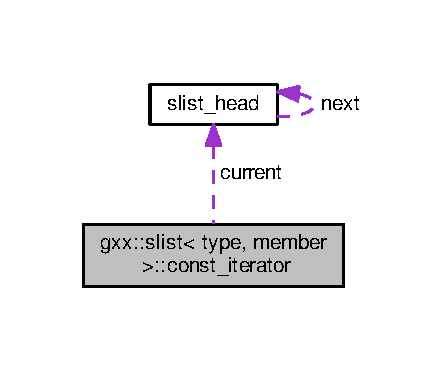
\includegraphics[width=213pt]{classgxx_1_1slist_1_1const__iterator__coll__graph}
\end{center}
\end{figure}
\subsection*{Public Types}
\begin{DoxyCompactItemize}
\item 
using {\bfseries value\+\_\+type} = type\hypertarget{classgxx_1_1slist_1_1const__iterator_a61d5f20481475a45a99c2936e573c445}{}\label{classgxx_1_1slist_1_1const__iterator_a61d5f20481475a45a99c2936e573c445}

\item 
using {\bfseries difference\+\_\+type} = ptrdiff\+\_\+t\hypertarget{classgxx_1_1slist_1_1const__iterator_ac519aa98365df7f3db71f9bd1b4997b1}{}\label{classgxx_1_1slist_1_1const__iterator_ac519aa98365df7f3db71f9bd1b4997b1}

\item 
using {\bfseries pointer} = type $\ast$\hypertarget{classgxx_1_1slist_1_1const__iterator_a3a134bb519f5a5bec184e701dbf1a7a6}{}\label{classgxx_1_1slist_1_1const__iterator_a3a134bb519f5a5bec184e701dbf1a7a6}

\item 
using {\bfseries reference} = type \&\hypertarget{classgxx_1_1slist_1_1const__iterator_a148e080572b609687c5cf215152165a4}{}\label{classgxx_1_1slist_1_1const__iterator_a148e080572b609687c5cf215152165a4}

\end{DoxyCompactItemize}
\subsection*{Public Member Functions}
\begin{DoxyCompactItemize}
\item 
{\bfseries const\+\_\+iterator} (\hyperlink{structslist__head}{slist\+\_\+head} $\ast$head)\hypertarget{classgxx_1_1slist_1_1const__iterator_a52efa55198cac3ace321fdf8a9e60c5f}{}\label{classgxx_1_1slist_1_1const__iterator_a52efa55198cac3ace321fdf8a9e60c5f}

\item 
{\bfseries const\+\_\+iterator} (const \hyperlink{classgxx_1_1slist_1_1const__iterator}{const\+\_\+iterator} \&other)\hypertarget{classgxx_1_1slist_1_1const__iterator_acae0adf68107be14ad8506396e8881b5}{}\label{classgxx_1_1slist_1_1const__iterator_acae0adf68107be14ad8506396e8881b5}

\item 
\hyperlink{classgxx_1_1slist_1_1const__iterator}{const\+\_\+iterator} {\bfseries operator++} (int)\hypertarget{classgxx_1_1slist_1_1const__iterator_a4ea3d9068543d23140cbb1df5b64596e}{}\label{classgxx_1_1slist_1_1const__iterator_a4ea3d9068543d23140cbb1df5b64596e}

\item 
\hyperlink{classgxx_1_1slist_1_1const__iterator}{const\+\_\+iterator} {\bfseries operator++} ()\hypertarget{classgxx_1_1slist_1_1const__iterator_aeac7167bc8cd22b1c890a15434ce3d7a}{}\label{classgxx_1_1slist_1_1const__iterator_aeac7167bc8cd22b1c890a15434ce3d7a}

\item 
bool {\bfseries operator!=} (const \hyperlink{classgxx_1_1slist_1_1const__iterator}{const\+\_\+iterator} \&b)\hypertarget{classgxx_1_1slist_1_1const__iterator_adbb9b9b03d09dd1033c35900a48f3c18}{}\label{classgxx_1_1slist_1_1const__iterator_adbb9b9b03d09dd1033c35900a48f3c18}

\item 
bool {\bfseries operator==} (const \hyperlink{classgxx_1_1slist_1_1const__iterator}{const\+\_\+iterator} \&b)\hypertarget{classgxx_1_1slist_1_1const__iterator_a201475b5b717a68cf8c70c6fa6be0e98}{}\label{classgxx_1_1slist_1_1const__iterator_a201475b5b717a68cf8c70c6fa6be0e98}

\item 
const type \& {\bfseries operator$\ast$} ()\hypertarget{classgxx_1_1slist_1_1const__iterator_a65991b69b62299d512e3221ce18cfc0e}{}\label{classgxx_1_1slist_1_1const__iterator_a65991b69b62299d512e3221ce18cfc0e}

\item 
const type $\ast$ {\bfseries operator-\/$>$} ()\hypertarget{classgxx_1_1slist_1_1const__iterator_a4f680c9c70cc9a623cc7c8833033e663}{}\label{classgxx_1_1slist_1_1const__iterator_a4f680c9c70cc9a623cc7c8833033e663}

\end{DoxyCompactItemize}
\subsection*{Public Attributes}
\begin{DoxyCompactItemize}
\item 
\hyperlink{structslist__head}{slist\+\_\+head} $\ast$ {\bfseries current}\hypertarget{classgxx_1_1slist_1_1const__iterator_a46b8690bd78c2e94eb7577386269216b}{}\label{classgxx_1_1slist_1_1const__iterator_a46b8690bd78c2e94eb7577386269216b}

\end{DoxyCompactItemize}


The documentation for this class was generated from the following file\+:\begin{DoxyCompactItemize}
\item 
/home/rfmeas/project/gxx/gxx/slist.\+h\end{DoxyCompactItemize}

\hypertarget{structmalgo_1_1const__step__ptr}{}\section{malgo\+:\+:const\+\_\+step\+\_\+ptr$<$ T $>$ Struct Template Reference}
\label{structmalgo_1_1const__step__ptr}\index{malgo\+::const\+\_\+step\+\_\+ptr$<$ T $>$@{malgo\+::const\+\_\+step\+\_\+ptr$<$ T $>$}}
\subsection*{Public Member Functions}
\begin{DoxyCompactItemize}
\item 
{\bfseries const\+\_\+step\+\_\+ptr} (const T $\ast$ptr, int step)\hypertarget{structmalgo_1_1const__step__ptr_a23e46253b0b02bb6fdcc6b217a67bff3}{}\label{structmalgo_1_1const__step__ptr_a23e46253b0b02bb6fdcc6b217a67bff3}

\item 
\hyperlink{structmalgo_1_1const__step__ptr}{const\+\_\+step\+\_\+ptr} \& {\bfseries operator++} ()\hypertarget{structmalgo_1_1const__step__ptr_a908655e3fc12b234a602e3685b73bca2}{}\label{structmalgo_1_1const__step__ptr_a908655e3fc12b234a602e3685b73bca2}

\item 
\hyperlink{structmalgo_1_1const__step__ptr}{const\+\_\+step\+\_\+ptr} {\bfseries operator++} (int)\hypertarget{structmalgo_1_1const__step__ptr_ae953f93da99ce9b85cbe548780ac9756}{}\label{structmalgo_1_1const__step__ptr_ae953f93da99ce9b85cbe548780ac9756}

\item 
const T \& {\bfseries operator$\ast$} ()\hypertarget{structmalgo_1_1const__step__ptr_a0aab3db1cbe52957a2cc270ac4d56268}{}\label{structmalgo_1_1const__step__ptr_a0aab3db1cbe52957a2cc270ac4d56268}

\item 
bool {\bfseries operator!=} (const \hyperlink{structmalgo_1_1const__step__ptr}{const\+\_\+step\+\_\+ptr} \&oth)\hypertarget{structmalgo_1_1const__step__ptr_ad0440de775e28d4ba0200eae455ce0f0}{}\label{structmalgo_1_1const__step__ptr_ad0440de775e28d4ba0200eae455ce0f0}

\end{DoxyCompactItemize}
\subsection*{Public Attributes}
\begin{DoxyCompactItemize}
\item 
const T $\ast$ {\bfseries ptr}\hypertarget{structmalgo_1_1const__step__ptr_ac93b86fa0c874d4ce33cff5059a3e325}{}\label{structmalgo_1_1const__step__ptr_ac93b86fa0c874d4ce33cff5059a3e325}

\item 
int {\bfseries step}\hypertarget{structmalgo_1_1const__step__ptr_afe0a9a2d33b3cf91c522c7ea73729f17}{}\label{structmalgo_1_1const__step__ptr_afe0a9a2d33b3cf91c522c7ea73729f17}

\end{DoxyCompactItemize}


The documentation for this struct was generated from the following file\+:\begin{DoxyCompactItemize}
\item 
/home/rfmeas/project/gxx/gxx/math/malgo.\+h\end{DoxyCompactItemize}

\hypertarget{classgxx_1_1controlled}{}\section{gxx\+:\+:controlled Class Reference}
\label{classgxx_1_1controlled}\index{gxx\+::controlled@{gxx\+::controlled}}
\subsection*{Public Member Functions}
\begin{DoxyCompactItemize}
\item 
void {\bfseries unlink\+\_\+controller} ()\hypertarget{classgxx_1_1controlled_a46a96a83461e8d5f48f93a462f8d86e4}{}\label{classgxx_1_1controlled_a46a96a83461e8d5f48f93a462f8d86e4}

\item 
void {\bfseries link\+\_\+controller} (\hyperlink{classgxx_1_1controller}{controller} $\ast$\+\_\+cntrl)\hypertarget{classgxx_1_1controlled_adb6c7f74eaef8754695c4f7df5dee916}{}\label{classgxx_1_1controlled_adb6c7f74eaef8754695c4f7df5dee916}

\item 
\hyperlink{classgxx_1_1controller}{controller} $\ast$ {\bfseries controller\+\_\+ptr} ()\hypertarget{classgxx_1_1controlled_a01e3b6f774453d1eabe431556b7ea825}{}\label{classgxx_1_1controlled_a01e3b6f774453d1eabe431556b7ea825}

\end{DoxyCompactItemize}


The documentation for this class was generated from the following file\+:\begin{DoxyCompactItemize}
\item 
/home/rfmeas/project/gxx/gxx/controlling.\+h\end{DoxyCompactItemize}

\hypertarget{classgxx_1_1controller}{}\section{gxx\+:\+:controller Class Reference}
\label{classgxx_1_1controller}\index{gxx\+::controller@{gxx\+::controller}}


Collaboration diagram for gxx\+:\+:controller\+:
\nopagebreak
\begin{figure}[H]
\begin{center}
\leavevmode
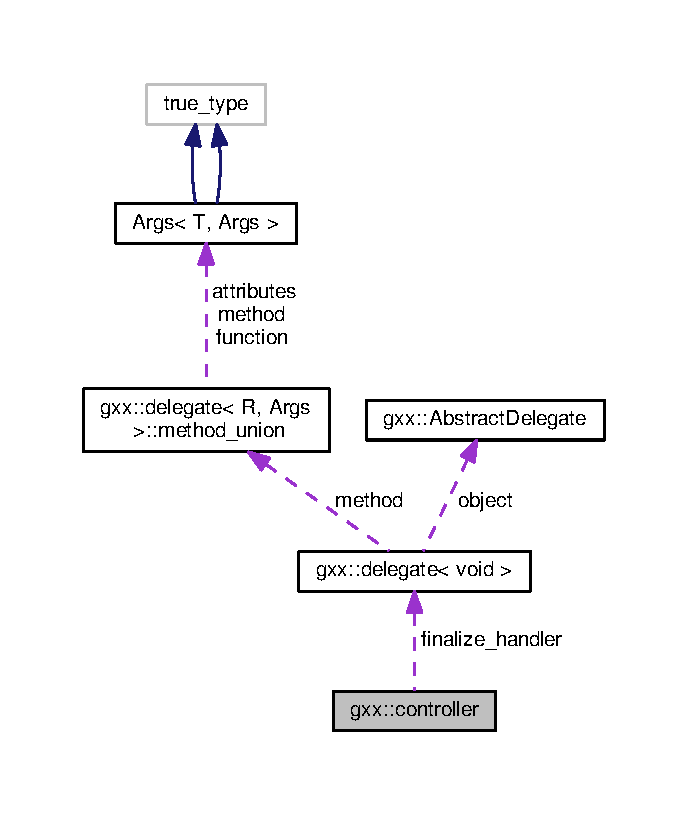
\includegraphics[width=330pt]{classgxx_1_1controller__coll__graph}
\end{center}
\end{figure}
\subsection*{Public Types}
\begin{DoxyCompactItemize}
\item 
enum {\bfseries state} \{ {\bfseries W\+O\+R\+K\+ED}, 
{\bfseries S\+T\+O\+P\+ED}, 
{\bfseries F\+I\+N\+I\+S\+H\+ED}
 \}\hypertarget{classgxx_1_1controller_ac07045ccbd72c2b4de4636962487c876}{}\label{classgxx_1_1controller_ac07045ccbd72c2b4de4636962487c876}

\end{DoxyCompactItemize}
\subsection*{Public Member Functions}
\begin{DoxyCompactItemize}
\item 
void {\bfseries finalize} ()\hypertarget{classgxx_1_1controller_ae34771ff9211cc037081c47df5ff53ce}{}\label{classgxx_1_1controller_ae34771ff9211cc037081c47df5ff53ce}

\item 
void {\bfseries set\+\_\+finalize\+\_\+handler} (\hyperlink{classgxx_1_1delegate}{gxx\+::action} act)\hypertarget{classgxx_1_1controller_aa078f0e51f2a6ea029c914a84bdbbac8}{}\label{classgxx_1_1controller_aa078f0e51f2a6ea029c914a84bdbbac8}

\item 
void {\bfseries set\+\_\+work\+\_\+state} ()\hypertarget{classgxx_1_1controller_a06d38fbd0f11938c16c94299db8201e1}{}\label{classgxx_1_1controller_a06d38fbd0f11938c16c94299db8201e1}

\item 
const char $\ast$ {\bfseries statestr} ()\hypertarget{classgxx_1_1controller_aadf433685594ab166f94a6cef80845f2}{}\label{classgxx_1_1controller_aadf433685594ab166f94a6cef80845f2}

\end{DoxyCompactItemize}
\subsection*{Public Attributes}
\begin{DoxyCompactItemize}
\item 
state {\bfseries \+\_\+state} = state\+::\+S\+T\+O\+P\+ED\hypertarget{classgxx_1_1controller_a42a5dab49c033e9998e8acd90d801bf4}{}\label{classgxx_1_1controller_a42a5dab49c033e9998e8acd90d801bf4}

\item 
\hyperlink{classgxx_1_1delegate}{gxx\+::action} {\bfseries finalize\+\_\+handler}\hypertarget{classgxx_1_1controller_a365dc6aee9ece7677c40ed77d2053da1}{}\label{classgxx_1_1controller_a365dc6aee9ece7677c40ed77d2053da1}

\end{DoxyCompactItemize}


The documentation for this class was generated from the following file\+:\begin{DoxyCompactItemize}
\item 
/home/rfmeas/project/gxx/gxx/controlling.\+h\end{DoxyCompactItemize}

\hypertarget{structinternal_1_1ConvertHelper}{}\section{internal\+:\+:Convert\+Helper$<$ From, To $>$ Struct Template Reference}
\label{structinternal_1_1ConvertHelper}\index{internal\+::\+Convert\+Helper$<$ From, To $>$@{internal\+::\+Convert\+Helper$<$ From, To $>$}}
\subsection*{Static Public Member Functions}
\begin{DoxyCompactItemize}
\item 
static \hyperlink{structsmall__}{small\+\_\+} {\bfseries Test} (To)\hypertarget{structinternal_1_1ConvertHelper_a07e36f50c2636da7b7529f2c43e09023}{}\label{structinternal_1_1ConvertHelper_a07e36f50c2636da7b7529f2c43e09023}

\item 
static \hyperlink{structbig__}{big\+\_\+} {\bfseries Test} (...)\hypertarget{structinternal_1_1ConvertHelper_a83c7c2d2612aa9954b26a6f6710eac9d}{}\label{structinternal_1_1ConvertHelper_a83c7c2d2612aa9954b26a6f6710eac9d}

\item 
static From {\bfseries Create} ()\hypertarget{structinternal_1_1ConvertHelper_a111a307f49b614d29529e5cb8280acd9}{}\label{structinternal_1_1ConvertHelper_a111a307f49b614d29529e5cb8280acd9}

\item 
static \hyperlink{structsmall__}{small\+\_\+} {\bfseries Test} (To)\hypertarget{structinternal_1_1ConvertHelper_a07e36f50c2636da7b7529f2c43e09023}{}\label{structinternal_1_1ConvertHelper_a07e36f50c2636da7b7529f2c43e09023}

\item 
static \hyperlink{structbig__}{big\+\_\+} {\bfseries Test} (...)\hypertarget{structinternal_1_1ConvertHelper_a83c7c2d2612aa9954b26a6f6710eac9d}{}\label{structinternal_1_1ConvertHelper_a83c7c2d2612aa9954b26a6f6710eac9d}

\item 
static From {\bfseries Create} ()\hypertarget{structinternal_1_1ConvertHelper_a111a307f49b614d29529e5cb8280acd9}{}\label{structinternal_1_1ConvertHelper_a111a307f49b614d29529e5cb8280acd9}

\end{DoxyCompactItemize}


The documentation for this struct was generated from the following file\+:\begin{DoxyCompactItemize}
\item 
/home/rfmeas/project/gxx/gxx/\+H\+I\+D\+E/utility/type\+\_\+relation.\+hpp\end{DoxyCompactItemize}

\hypertarget{classgxx_1_1math_1_1coord1__compact}{}\section{gxx\+:\+:math\+:\+:coord1\+\_\+compact Class Reference}
\label{classgxx_1_1math_1_1coord1__compact}\index{gxx\+::math\+::coord1\+\_\+compact@{gxx\+::math\+::coord1\+\_\+compact}}


The documentation for this class was generated from the following file\+:\begin{DoxyCompactItemize}
\item 
/home/rfmeas/project/gxx/gxx/math/major.\+h\end{DoxyCompactItemize}

\hypertarget{classgxx_1_1math_1_1coord2__compact}{}\section{gxx\+:\+:math\+:\+:coord2\+\_\+compact Class Reference}
\label{classgxx_1_1math_1_1coord2__compact}\index{gxx\+::math\+::coord2\+\_\+compact@{gxx\+::math\+::coord2\+\_\+compact}}


The documentation for this class was generated from the following file\+:\begin{DoxyCompactItemize}
\item 
/home/rfmeas/project/gxx/gxx/math/major.\+h\end{DoxyCompactItemize}

\hypertarget{classgxx_1_1ngeom_1_1coordinates}{}\section{gxx\+:\+:ngeom\+:\+:coordinates Class Reference}
\label{classgxx_1_1ngeom_1_1coordinates}\index{gxx\+::ngeom\+::coordinates@{gxx\+::ngeom\+::coordinates}}


Inheritance diagram for gxx\+:\+:ngeom\+:\+:coordinates\+:
% FIG 0


Collaboration diagram for gxx\+:\+:ngeom\+:\+:coordinates\+:
% FIG 1
\subsection*{Public Member Functions}
\begin{DoxyCompactItemize}
\item 
{\bfseries coordinates} (size\+\_\+t size)\hypertarget{classgxx_1_1ngeom_1_1coordinates_a59e2d7b6290bd5288e0b95539a41bd14}{}\label{classgxx_1_1ngeom_1_1coordinates_a59e2d7b6290bd5288e0b95539a41bd14}

\item 
{\bfseries coordinates} (\hyperlink{classgxx_1_1object__buffer}{gxx\+::objbuf}$<$ double $>$ buf)\hypertarget{classgxx_1_1ngeom_1_1coordinates_aa53f4baae93c26af40459d07ebc09600}{}\label{classgxx_1_1ngeom_1_1coordinates_aa53f4baae93c26af40459d07ebc09600}

\item 
{\bfseries coordinates} (const std\+::initializer\+\_\+list$<$ double $>$ \&buf)\hypertarget{classgxx_1_1ngeom_1_1coordinates_a6c5916f60a54f73e3315dc8f94c127b9}{}\label{classgxx_1_1ngeom_1_1coordinates_a6c5916f60a54f73e3315dc8f94c127b9}

\item 
{\bfseries coordinates} (const \hyperlink{classgxx_1_1ngeom_1_1coordinates}{coordinates} \&)=default\hypertarget{classgxx_1_1ngeom_1_1coordinates_a16c22038643673ea03773792a7fe72ff}{}\label{classgxx_1_1ngeom_1_1coordinates_a16c22038643673ea03773792a7fe72ff}

\item 
{\bfseries coordinates} (\hyperlink{classgxx_1_1ngeom_1_1coordinates}{coordinates} \&\&)=default\hypertarget{classgxx_1_1ngeom_1_1coordinates_ab8e18c964d42d35b191edf521a2a0200}{}\label{classgxx_1_1ngeom_1_1coordinates_ab8e18c964d42d35b191edf521a2a0200}

\item 
size\+\_\+t {\bfseries dim} () const \hypertarget{classgxx_1_1ngeom_1_1coordinates_af78809d856d39a9521e8f862bda570e5}{}\label{classgxx_1_1ngeom_1_1coordinates_af78809d856d39a9521e8f862bda570e5}

\end{DoxyCompactItemize}
\subsection*{Additional Inherited Members}


The documentation for this class was generated from the following file\+:\begin{DoxyCompactItemize}
\item 
/home/rfmeas/project/gxx/gxx/geom/ngeom.\+h\end{DoxyCompactItemize}

\hypertarget{classgxx_1_1creader}{}\section{gxx\+:\+:creader Class Reference}
\label{classgxx_1_1creader}\index{gxx\+::creader@{gxx\+::creader}}
\subsection*{Public Member Functions}
\begin{DoxyCompactItemize}
\item 
{\bfseries creader} (const char $\ast$\+\_\+ptr)\hypertarget{classgxx_1_1creader_a3d64f1c6c8ff097b418d7e4c6da53d0f}{}\label{classgxx_1_1creader_a3d64f1c6c8ff097b418d7e4c6da53d0f}

\item 
{\footnotesize template$<$typename Functor $>$ }\\std\+::string {\bfseries string\+\_\+while} (Functor \&\&func)\hypertarget{classgxx_1_1creader_a1261c0ee4f6f3854bd66f0b340527257}{}\label{classgxx_1_1creader_a1261c0ee4f6f3854bd66f0b340527257}

\item 
{\footnotesize template$<$typename Functor $>$ }\\bool {\bfseries next\+\_\+is} (Functor \&\&func)\hypertarget{classgxx_1_1creader_af64d9c78ecc868146940e5a9566ab531}{}\label{classgxx_1_1creader_af64d9c78ecc868146940e5a9566ab531}

\item 
bool {\bfseries next\+\_\+is} (char c)\hypertarget{classgxx_1_1creader_a375bdf305321c4c0156d0ebbc0fa8174}{}\label{classgxx_1_1creader_a375bdf305321c4c0156d0ebbc0fa8174}

\item 
bool {\bfseries next\+\_\+is} (\hyperlink{classgxx_1_1buffer}{gxx\+::buffer} smbs)\hypertarget{classgxx_1_1creader_a52b3516974e08f14dedb2cdd83cd686f}{}\label{classgxx_1_1creader_a52b3516974e08f14dedb2cdd83cd686f}

\item 
void {\bfseries skip} ()\hypertarget{classgxx_1_1creader_a3b1908b476a8ae52a484d6c3313e4043}{}\label{classgxx_1_1creader_a3b1908b476a8ae52a484d6c3313e4043}

\item 
{\footnotesize template$<$typename Functor $>$ }\\void {\bfseries skip\+\_\+while} (Functor \&\&func)\hypertarget{classgxx_1_1creader_a9438293285f7a90bfbd173a77d5b8eb4}{}\label{classgxx_1_1creader_a9438293285f7a90bfbd173a77d5b8eb4}

\item 
void {\bfseries skip\+\_\+while} (const char $\ast$smbs)\hypertarget{classgxx_1_1creader_ae2f003d928c118a62029303ccb09a18f}{}\label{classgxx_1_1creader_ae2f003d928c118a62029303ccb09a18f}

\item 
void {\bfseries skip\+\_\+while} (char smb)\hypertarget{classgxx_1_1creader_ad408f67fe181235640b1fcd8c6141c50}{}\label{classgxx_1_1creader_ad408f67fe181235640b1fcd8c6141c50}

\item 
int {\bfseries integer} ()\hypertarget{classgxx_1_1creader_a7aeef0969b937dca7c314bf95f9f51c1}{}\label{classgxx_1_1creader_a7aeef0969b937dca7c314bf95f9f51c1}

\end{DoxyCompactItemize}


The documentation for this class was generated from the following file\+:\begin{DoxyCompactItemize}
\item 
/home/rfmeas/project/gxx/gxx/creader.\+h\end{DoxyCompactItemize}

\hypertarget{structrabbit_1_1crvcrv__analytic__intresult}{}\section{rabbit\+:\+:crvcrv\+\_\+analytic\+\_\+intresult Struct Reference}
\label{structrabbit_1_1crvcrv__analytic__intresult}\index{rabbit\+::crvcrv\+\_\+analytic\+\_\+intresult@{rabbit\+::crvcrv\+\_\+analytic\+\_\+intresult}}
\subsection*{Public Member Functions}
\begin{DoxyCompactItemize}
\item 
bool {\bfseries have\+\_\+points} () const \hypertarget{structrabbit_1_1crvcrv__analytic__intresult_aac53ba39966aea9b14e45f54a23a150a}{}\label{structrabbit_1_1crvcrv__analytic__intresult_aac53ba39966aea9b14e45f54a23a150a}

\item 
{\bfseries crvcrv\+\_\+analytic\+\_\+intresult} (bool b)\hypertarget{structrabbit_1_1crvcrv__analytic__intresult_aaf8e0f2e035adb449e974ced8bdb1839}{}\label{structrabbit_1_1crvcrv__analytic__intresult_aaf8e0f2e035adb449e974ced8bdb1839}

\item 
{\bfseries crvcrv\+\_\+analytic\+\_\+intresult} (bool b, double offset, bool revdir)\hypertarget{structrabbit_1_1crvcrv__analytic__intresult_a2163f242cbae53dce317a41e89096fd1}{}\label{structrabbit_1_1crvcrv__analytic__intresult_a2163f242cbae53dce317a41e89096fd1}

\item 
{\bfseries crvcrv\+\_\+analytic\+\_\+intresult} (const std\+::initializer\+\_\+list$<$ double $>$ \&ap, const std\+::initializer\+\_\+list$<$ double $>$ \&bp, const std\+::initializer\+\_\+list$<$ \hyperlink{classmalgo_1_1vector2}{point2} $>$ \&p)\hypertarget{structrabbit_1_1crvcrv__analytic__intresult_a0dd00361b8cb546744907121a222337f}{}\label{structrabbit_1_1crvcrv__analytic__intresult_a0dd00361b8cb546744907121a222337f}

\item 
\hyperlink{structrabbit_1_1crvcrv__analytic__intresult}{crvcrv\+\_\+analytic\+\_\+intresult} \& {\bfseries swap\+\_\+curves} ()\hypertarget{structrabbit_1_1crvcrv__analytic__intresult_a8c50f3a1948ca5e1866aa016d454108f}{}\label{structrabbit_1_1crvcrv__analytic__intresult_a8c50f3a1948ca5e1866aa016d454108f}

\item 
bool {\bfseries empty} ()\hypertarget{structrabbit_1_1crvcrv__analytic__intresult_a0dc8e84861c424657203d47404337153}{}\label{structrabbit_1_1crvcrv__analytic__intresult_a0dc8e84861c424657203d47404337153}

\item 
size\+\_\+t {\bfseries print\+To} (\hyperlink{classgxx_1_1io_1_1ostream}{gxx\+::io\+::ostream} \&o) const \hypertarget{structrabbit_1_1crvcrv__analytic__intresult_a09daed1c771ee268480087e428e82948}{}\label{structrabbit_1_1crvcrv__analytic__intresult_a09daed1c771ee268480087e428e82948}

\end{DoxyCompactItemize}
\subsection*{Public Attributes}
\begin{DoxyCompactItemize}
\item 
std\+::vector$<$ double $>$ {\bfseries apnts}\hypertarget{structrabbit_1_1crvcrv__analytic__intresult_a66b03a0b14c3f4bb821bc03d7042d318}{}\label{structrabbit_1_1crvcrv__analytic__intresult_a66b03a0b14c3f4bb821bc03d7042d318}

\item 
std\+::vector$<$ double $>$ {\bfseries bpnts}\hypertarget{structrabbit_1_1crvcrv__analytic__intresult_a532dcc723b2913a351749e42ceeecad0}{}\label{structrabbit_1_1crvcrv__analytic__intresult_a532dcc723b2913a351749e42ceeecad0}

\item 
std\+::vector$<$ \hyperlink{classmalgo_1_1vector2}{point2} $>$ {\bfseries pnts}\hypertarget{structrabbit_1_1crvcrv__analytic__intresult_a8d93adf1e9c7a29330f89e6744377686}{}\label{structrabbit_1_1crvcrv__analytic__intresult_a8d93adf1e9c7a29330f89e6744377686}

\item 
bool {\bfseries same} = false\hypertarget{structrabbit_1_1crvcrv__analytic__intresult_a7159b0e37296a857f39fbdebe0615106}{}\label{structrabbit_1_1crvcrv__analytic__intresult_a7159b0e37296a857f39fbdebe0615106}

\item 
double {\bfseries offset}\hypertarget{structrabbit_1_1crvcrv__analytic__intresult_ab853796ef10056a14f42b04626dc5da6}{}\label{structrabbit_1_1crvcrv__analytic__intresult_ab853796ef10056a14f42b04626dc5da6}

\item 
bool {\bfseries revdir}\hypertarget{structrabbit_1_1crvcrv__analytic__intresult_ab58dbcadf7dfb53a29730e493255fb8d}{}\label{structrabbit_1_1crvcrv__analytic__intresult_ab58dbcadf7dfb53a29730e493255fb8d}

\end{DoxyCompactItemize}


The documentation for this struct was generated from the following file\+:\begin{DoxyCompactItemize}
\item 
/home/rfmeas/project/gxx/gxx/rabbit/crvints.\+cpp\end{DoxyCompactItemize}

\hypertarget{classgxx_1_1cstring}{}\section{gxx\+:\+:cstring Class Reference}
\label{classgxx_1_1cstring}\index{gxx\+::cstring@{gxx\+::cstring}}
\subsection*{Public Member Functions}
\begin{DoxyCompactItemize}
\item 
{\bfseries cstring} (const char $\ast$ptr)\hypertarget{classgxx_1_1cstring_a4803ee530431722ba9dbeb212d052896}{}\label{classgxx_1_1cstring_a4803ee530431722ba9dbeb212d052896}

\item 
bool {\bfseries operator==} (const char $\ast$oth)\hypertarget{classgxx_1_1cstring_a6f521cc316fbb56313fef754bfa7dde4}{}\label{classgxx_1_1cstring_a6f521cc316fbb56313fef754bfa7dde4}

\item 
bool {\bfseries operator==} (const \hyperlink{classgxx_1_1cstring}{cstring} oth)\hypertarget{classgxx_1_1cstring_a4c81f9d963e87eae1d19d8a8ddb8eba8}{}\label{classgxx_1_1cstring_a4c81f9d963e87eae1d19d8a8ddb8eba8}

\item 
const char $\ast$ {\bfseries data} () const \hypertarget{classgxx_1_1cstring_a818fb4318548e1b397f548d1193ac3e3}{}\label{classgxx_1_1cstring_a818fb4318548e1b397f548d1193ac3e3}

\item 
size\+\_\+t {\bfseries size} () const \hypertarget{classgxx_1_1cstring_a66b41fae9f124dbfb36cc6ed1a65fde7}{}\label{classgxx_1_1cstring_a66b41fae9f124dbfb36cc6ed1a65fde7}

\end{DoxyCompactItemize}
\subsection*{Public Attributes}
\begin{DoxyCompactItemize}
\item 
const char $\ast$const {\bfseries ptr}\hypertarget{classgxx_1_1cstring_a4a13d7b0c5eb2f49799e97f4aefcec96}{}\label{classgxx_1_1cstring_a4a13d7b0c5eb2f49799e97f4aefcec96}

\end{DoxyCompactItemize}


The documentation for this class was generated from the following file\+:\begin{DoxyCompactItemize}
\item 
/home/rfmeas/project/gxx/gxx/cstring.\+h\end{DoxyCompactItemize}

\hypertarget{classgxx_1_1geom2_1_1curve}{}\section{gxx\+:\+:geom2\+:\+:curve Class Reference}
\label{classgxx_1_1geom2_1_1curve}\index{gxx\+::geom2\+::curve@{gxx\+::geom2\+::curve}}


Inheritance diagram for gxx\+:\+:geom2\+:\+:curve\+:
\nopagebreak
\begin{figure}[H]
\begin{center}
\leavevmode
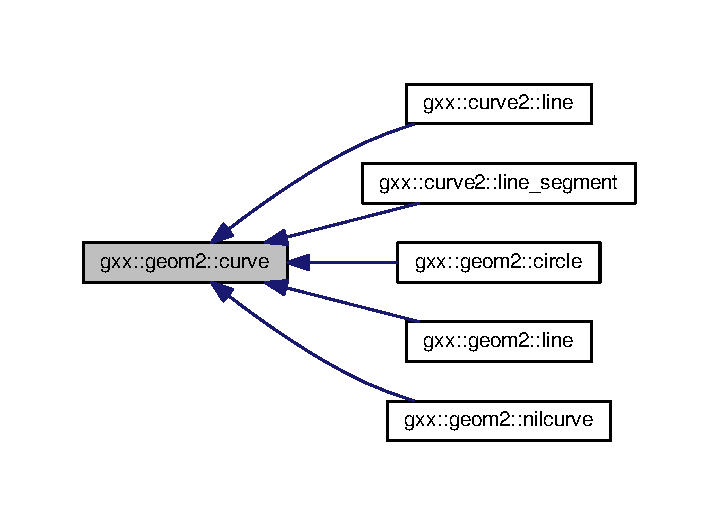
\includegraphics[width=345pt]{classgxx_1_1geom2_1_1curve__inherit__graph}
\end{center}
\end{figure}
\subsection*{Public Member Functions}
\begin{DoxyCompactItemize}
\item 
virtual \hyperlink{classmalgo_1_1vector2}{point} {\bfseries d0} (double t) const =0\hypertarget{classgxx_1_1geom2_1_1curve_a66cb70e2231790cfad01ccbde44e5386}{}\label{classgxx_1_1geom2_1_1curve_a66cb70e2231790cfad01ccbde44e5386}

\item 
virtual \hyperlink{classmalgo_1_1vector2}{vector} {\bfseries d1} (double t) const =0\hypertarget{classgxx_1_1geom2_1_1curve_a9420622691b23230d2abb55053892253}{}\label{classgxx_1_1geom2_1_1curve_a9420622691b23230d2abb55053892253}

\item 
virtual bool {\bfseries is\+\_\+closed} ()\hypertarget{classgxx_1_1geom2_1_1curve_a2a66df08c2ea61834f4f3c4a534d4486}{}\label{classgxx_1_1geom2_1_1curve_a2a66df08c2ea61834f4f3c4a534d4486}

\item 
virtual bool {\bfseries is\+\_\+periodic} ()\hypertarget{classgxx_1_1geom2_1_1curve_ab5c6e8656bb94e707347ef759f16e983}{}\label{classgxx_1_1geom2_1_1curve_ab5c6e8656bb94e707347ef759f16e983}

\item 
virtual double {\bfseries tmin} ()\hypertarget{classgxx_1_1geom2_1_1curve_a373183153d480ef8d9b07902f1ace1a1}{}\label{classgxx_1_1geom2_1_1curve_a373183153d480ef8d9b07902f1ace1a1}

\item 
virtual double {\bfseries tmax} ()\hypertarget{classgxx_1_1geom2_1_1curve_a8d471bd51d4cdc60f149be693214fb5a}{}\label{classgxx_1_1geom2_1_1curve_a8d471bd51d4cdc60f149be693214fb5a}

\item 
virtual double {\bfseries rotation\+\_\+angle} () const \hypertarget{classgxx_1_1geom2_1_1curve_a26efbda8dcf5d280a173f19c65d841c0}{}\label{classgxx_1_1geom2_1_1curve_a26efbda8dcf5d280a173f19c65d841c0}

\item 
virtual size\+\_\+t {\bfseries print\+To} (\hyperlink{classgxx_1_1io_1_1ostream}{gxx\+::io\+::ostream} \&o) const \hypertarget{classgxx_1_1geom2_1_1curve_a7b2b797ae4e46c0f8d8afd34fa96b7b2}{}\label{classgxx_1_1geom2_1_1curve_a7b2b797ae4e46c0f8d8afd34fa96b7b2}

\item 
virtual void {\bfseries draw\+To} (\hyperlink{classgxx_1_1drawer2d}{drawer2d} \&cntxt) const \hypertarget{classgxx_1_1geom2_1_1curve_a46cca40ecc2dbdd16b7c03bcee4459d3}{}\label{classgxx_1_1geom2_1_1curve_a46cca40ecc2dbdd16b7c03bcee4459d3}

\item 
virtual \hyperlink{structgxx_1_1geom2_1_1boundbox}{boundbox} {\bfseries getbound} (double s, double f) const \hypertarget{classgxx_1_1geom2_1_1curve_a7c6d834c3fb4e5a7b67965a48631bd41}{}\label{classgxx_1_1geom2_1_1curve_a7c6d834c3fb4e5a7b67965a48631bd41}

\item 
virtual \hyperlink{structgxx_1_1geom2_1_1boundbox}{boundbox} {\bfseries getbound} (const \hyperlink{classgxx_1_1math_1_1interval}{math\+::interval}$<$ double $>$ \&t) const \hypertarget{classgxx_1_1geom2_1_1curve_a7e13d3fcd4107ae44cbb77374c70ff46}{}\label{classgxx_1_1geom2_1_1curve_a7e13d3fcd4107ae44cbb77374c70ff46}

\item 
virtual bool {\bfseries is\+\_\+analityc} ()\hypertarget{classgxx_1_1geom2_1_1curve_ace29dec87aeaededcf8f6ad4d67aca23}{}\label{classgxx_1_1geom2_1_1curve_ace29dec87aeaededcf8f6ad4d67aca23}

\item 
virtual std\+::shared\+\_\+ptr$<$ \hyperlink{classgxx_1_1geom2_1_1curve}{curve} $>$ {\bfseries translate} (double x, double y)\hypertarget{classgxx_1_1geom2_1_1curve_a4d9d1bbdfba0a76a989043eaed94d078}{}\label{classgxx_1_1geom2_1_1curve_a4d9d1bbdfba0a76a989043eaed94d078}

\item 
virtual std\+::shared\+\_\+ptr$<$ \hyperlink{classgxx_1_1geom2_1_1curve}{curve} $>$ {\bfseries rotate} (double a)\hypertarget{classgxx_1_1geom2_1_1curve_a316c920a9348fb891a5b2324f9f3a355}{}\label{classgxx_1_1geom2_1_1curve_a316c920a9348fb891a5b2324f9f3a355}

\end{DoxyCompactItemize}


The documentation for this class was generated from the following file\+:\begin{DoxyCompactItemize}
\item 
/home/rfmeas/project/gxx/gxx/geom/geom2.\+h\end{DoxyCompactItemize}

\hypertarget{classgxx_1_1curve2_1_1curve}{}\section{gxx\+:\+:curve2\+:\+:curve Class Reference}
\label{classgxx_1_1curve2_1_1curve}\index{gxx\+::curve2\+::curve@{gxx\+::curve2\+::curve}}
\subsection*{Public Member Functions}
\begin{DoxyCompactItemize}
\item 
virtual \hyperlink{classmalgo_1_1vector2}{point} {\bfseries d0} (double t)=0\hypertarget{classgxx_1_1curve2_1_1curve_a9292d9f5a865812af902e2919f897498}{}\label{classgxx_1_1curve2_1_1curve_a9292d9f5a865812af902e2919f897498}

\item 
virtual \hyperlink{classmalgo_1_1vector2}{vector} {\bfseries d1} (double t)=0\hypertarget{classgxx_1_1curve2_1_1curve_a9e61f66c6d9fa0f3a2eef1bfae71f7c4}{}\label{classgxx_1_1curve2_1_1curve_a9e61f66c6d9fa0f3a2eef1bfae71f7c4}

\item 
virtual bool {\bfseries is\+\_\+closed} ()\hypertarget{classgxx_1_1curve2_1_1curve_a7d71fd12bda93d336846c87c4540015a}{}\label{classgxx_1_1curve2_1_1curve_a7d71fd12bda93d336846c87c4540015a}

\item 
virtual bool {\bfseries is\+\_\+periodic} ()\hypertarget{classgxx_1_1curve2_1_1curve_a71fd5539e811cddcebbe0ef233be33c6}{}\label{classgxx_1_1curve2_1_1curve_a71fd5539e811cddcebbe0ef233be33c6}

\item 
virtual double {\bfseries tmin} ()\hypertarget{classgxx_1_1curve2_1_1curve_a420e8364956a115c6523b35b7ab96213}{}\label{classgxx_1_1curve2_1_1curve_a420e8364956a115c6523b35b7ab96213}

\item 
virtual double {\bfseries tmax} ()\hypertarget{classgxx_1_1curve2_1_1curve_a3f78799e64c71ec4c86cb1bec8943f88}{}\label{classgxx_1_1curve2_1_1curve_a3f78799e64c71ec4c86cb1bec8943f88}

\item 
virtual size\+\_\+t {\bfseries print\+To} (\hyperlink{classgxx_1_1io_1_1ostream}{gxx\+::io\+::ostream} \&o) const \hypertarget{classgxx_1_1curve2_1_1curve_a79a3202da23c99f6f69426039bf1acd9}{}\label{classgxx_1_1curve2_1_1curve_a79a3202da23c99f6f69426039bf1acd9}

\end{DoxyCompactItemize}


The documentation for this class was generated from the following file\+:\begin{DoxyCompactItemize}
\item 
/home/rfmeas/project/gxx/gxx/geom/\+H\+I\+D\+E/curve2.\+h\end{DoxyCompactItemize}

\hypertarget{classgxx_1_1curve3_1_1curve}{}\section{gxx\+:\+:curve3\+:\+:curve Class Reference}
\label{classgxx_1_1curve3_1_1curve}\index{gxx\+::curve3\+::curve@{gxx\+::curve3\+::curve}}


Inheritance diagram for gxx\+:\+:curve3\+:\+:curve\+:
% FIG 0
\subsection*{Public Member Functions}
\begin{DoxyCompactItemize}
\item 
virtual \hyperlink{classgxx_1_1geom3_1_1point}{point} {\bfseries d0} (double t)=0\hypertarget{classgxx_1_1curve3_1_1curve_a84f0f6d4aeebe521e8e26e47459594d5}{}\label{classgxx_1_1curve3_1_1curve_a84f0f6d4aeebe521e8e26e47459594d5}

\item 
virtual bool {\bfseries is\+\_\+closed} ()\hypertarget{classgxx_1_1curve3_1_1curve_a379db289818f96a48aa84273fa32718f}{}\label{classgxx_1_1curve3_1_1curve_a379db289818f96a48aa84273fa32718f}

\item 
virtual bool {\bfseries is\+\_\+periodic} ()\hypertarget{classgxx_1_1curve3_1_1curve_ac19c573b85e6bff4b858071649c2fb14}{}\label{classgxx_1_1curve3_1_1curve_ac19c573b85e6bff4b858071649c2fb14}

\item 
virtual double {\bfseries tmin} ()\hypertarget{classgxx_1_1curve3_1_1curve_a46210bc3f70e1687fce994b84ab809be}{}\label{classgxx_1_1curve3_1_1curve_a46210bc3f70e1687fce994b84ab809be}

\item 
virtual double {\bfseries tmax} ()\hypertarget{classgxx_1_1curve3_1_1curve_a20e52a188719bd1c5eaac3a3c8d85283}{}\label{classgxx_1_1curve3_1_1curve_a20e52a188719bd1c5eaac3a3c8d85283}

\item 
virtual size\+\_\+t {\bfseries print\+To} (\hyperlink{classgxx_1_1io_1_1ostream}{gxx\+::io\+::ostream} \&o) const \hypertarget{classgxx_1_1curve3_1_1curve_aaedeec15809c75fb9973e49fab3fb3c0}{}\label{classgxx_1_1curve3_1_1curve_aaedeec15809c75fb9973e49fab3fb3c0}

\end{DoxyCompactItemize}


The documentation for this class was generated from the following file\+:\begin{DoxyCompactItemize}
\item 
/home/rfmeas/project/gxx/gxx/geom/\+H\+I\+D\+E/curve3.\+h\end{DoxyCompactItemize}

\hypertarget{classgxx_1_1ngeom_1_1curve}{}\section{gxx\+:\+:ngeom\+:\+:curve Class Reference}
\label{classgxx_1_1ngeom_1_1curve}\index{gxx\+::ngeom\+::curve@{gxx\+::ngeom\+::curve}}


Inheritance diagram for gxx\+:\+:ngeom\+:\+:curve\+:
\nopagebreak
\begin{figure}[H]
\begin{center}
\leavevmode
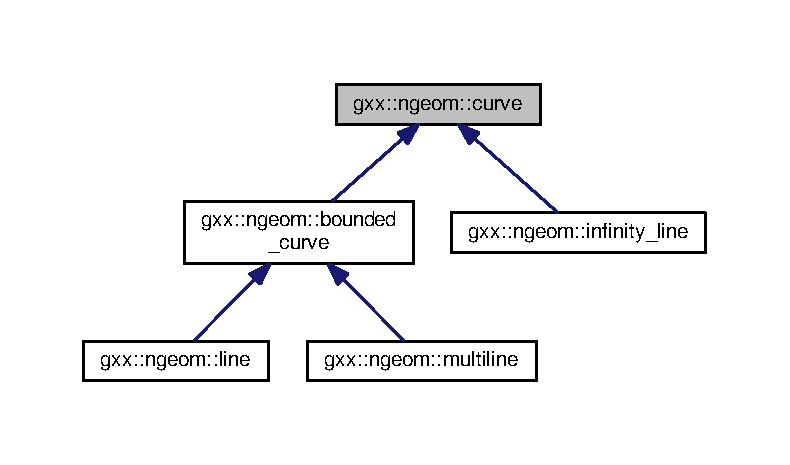
\includegraphics[width=350pt]{classgxx_1_1ngeom_1_1curve__inherit__graph}
\end{center}
\end{figure}
\subsection*{Public Member Functions}
\begin{DoxyCompactItemize}
\item 
virtual \hyperlink{classgxx_1_1ngeom_1_1point}{point} {\bfseries d0} (double t) const =0\hypertarget{classgxx_1_1ngeom_1_1curve_a0fc5baa675a79abdb0218338b2373719}{}\label{classgxx_1_1ngeom_1_1curve_a0fc5baa675a79abdb0218338b2373719}

\item 
virtual std\+::vector$<$ \hyperlink{classgxx_1_1ngeom_1_1point}{point} $>$ {\bfseries points\+\_\+with} (int num, double coord) const \hypertarget{classgxx_1_1ngeom_1_1curve_a9da6484cf7859a66753107e3d231abf4}{}\label{classgxx_1_1ngeom_1_1curve_a9da6484cf7859a66753107e3d231abf4}

\end{DoxyCompactItemize}


The documentation for this class was generated from the following file\+:\begin{DoxyCompactItemize}
\item 
/home/rfmeas/project/gxx/gxx/geom/ncurve.\+h\end{DoxyCompactItemize}

\hypertarget{classgxx_1_1topo2_1_1curve}{}\section{gxx\+:\+:topo2\+:\+:curve Class Reference}
\label{classgxx_1_1topo2_1_1curve}\index{gxx\+::topo2\+::curve@{gxx\+::topo2\+::curve}}
\subsection*{Public Member Functions}
\begin{DoxyCompactItemize}
\item 
void {\bfseries reserve} ()\hypertarget{classgxx_1_1topo2_1_1curve_ac8874c22cfbd9dc2585fb74d4bed7aaa}{}\label{classgxx_1_1topo2_1_1curve_ac8874c22cfbd9dc2585fb74d4bed7aaa}

\item 
\hyperlink{classmalgo_1_1vector2}{g2\+::point} {\bfseries start} ()\hypertarget{classgxx_1_1topo2_1_1curve_a8940d5a74bd568e3ef06dbbbdafe5502}{}\label{classgxx_1_1topo2_1_1curve_a8940d5a74bd568e3ef06dbbbdafe5502}

\item 
\hyperlink{classmalgo_1_1vector2}{g2\+::point} {\bfseries finish} ()\hypertarget{classgxx_1_1topo2_1_1curve_a0dd1586f5fe1ce3d92a8e5092d38f38d}{}\label{classgxx_1_1topo2_1_1curve_a0dd1586f5fe1ce3d92a8e5092d38f38d}

\item 
{\bfseries curve} (\hyperlink{classmalgo_1_1vector2}{g2\+::point} pnt1, \hyperlink{classmalgo_1_1vector2}{g2\+::point} pnt2)\hypertarget{classgxx_1_1topo2_1_1curve_a644b33558b85aebbc8a03d1180da7cf3}{}\label{classgxx_1_1topo2_1_1curve_a644b33558b85aebbc8a03d1180da7cf3}

\end{DoxyCompactItemize}
\subsection*{Public Attributes}
\begin{DoxyCompactItemize}
\item 
double {\bfseries bmin}\hypertarget{classgxx_1_1topo2_1_1curve_a7e5a2c4217df1f54ae490b22a9fd159b}{}\label{classgxx_1_1topo2_1_1curve_a7e5a2c4217df1f54ae490b22a9fd159b}

\item 
double {\bfseries bmax}\hypertarget{classgxx_1_1topo2_1_1curve_a5e7aefdadc57819ece97c8ce22bca3d4}{}\label{classgxx_1_1topo2_1_1curve_a5e7aefdadc57819ece97c8ce22bca3d4}

\end{DoxyCompactItemize}


The documentation for this class was generated from the following file\+:\begin{DoxyCompactItemize}
\item 
/home/rfmeas/project/gxx/gxx/geom/\+H\+I\+D\+E/topo2.\+h\end{DoxyCompactItemize}

\hypertarget{structcvector__t}{}\section{cvector\+\_\+t Struct Reference}
\label{structcvector__t}\index{cvector\+\_\+t@{cvector\+\_\+t}}


Collaboration diagram for cvector\+\_\+t\+:
\nopagebreak
\begin{figure}[H]
\begin{center}
\leavevmode
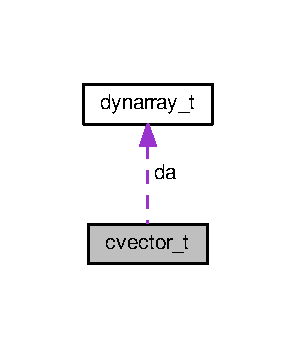
\includegraphics[width=142pt]{structcvector__t__coll__graph}
\end{center}
\end{figure}
\subsection*{Public Attributes}
\begin{DoxyCompactItemize}
\item 
\hyperlink{structdynarray__t}{dynarray\+\_\+t} {\bfseries da}\hypertarget{structcvector__t_a57787c5295a7fb99662be920235c14fc}{}\label{structcvector__t_a57787c5295a7fb99662be920235c14fc}

\item 
size\+\_\+t {\bfseries elsz}\hypertarget{structcvector__t_a5fbe091cf3647b5f6534fbc69529c1a8}{}\label{structcvector__t_a5fbe091cf3647b5f6534fbc69529c1a8}

\item 
size\+\_\+t {\bfseries sz}\hypertarget{structcvector__t_a07cb708e3aad0103fb99cf8baab92aa1}{}\label{structcvector__t_a07cb708e3aad0103fb99cf8baab92aa1}

\end{DoxyCompactItemize}


The documentation for this struct was generated from the following file\+:\begin{DoxyCompactItemize}
\item 
/home/rfmeas/project/gxx/gxx/datastruct/\+H\+I\+D\+E/cvector.\+h\end{DoxyCompactItemize}

\hypertarget{classgxx_1_1surf3_1_1cylinder}{}\section{gxx\+:\+:surf3\+:\+:cylinder Class Reference}
\label{classgxx_1_1surf3_1_1cylinder}\index{gxx\+::surf3\+::cylinder@{gxx\+::surf3\+::cylinder}}


Inheritance diagram for gxx\+:\+:surf3\+:\+:cylinder\+:
% FIG 0


Collaboration diagram for gxx\+:\+:surf3\+:\+:cylinder\+:
% FIG 1
\subsection*{Public Member Functions}
\begin{DoxyCompactItemize}
\item 
{\bfseries cylinder} (double r, double h, const \hyperlink{classgxx_1_1geom3_1_1axis3}{axis3} \&ax3)\hypertarget{classgxx_1_1surf3_1_1cylinder_a02c9f02f2d8be5aa7f3ca76253ca56a4}{}\label{classgxx_1_1surf3_1_1cylinder_a02c9f02f2d8be5aa7f3ca76253ca56a4}

\item 
\hyperlink{classgxx_1_1geom3_1_1point}{point} {\bfseries d0} (double v, double u)\hypertarget{classgxx_1_1surf3_1_1cylinder_a13d335090c4f2b1ef2d9d60211c0cf18}{}\label{classgxx_1_1surf3_1_1cylinder_a13d335090c4f2b1ef2d9d60211c0cf18}

\end{DoxyCompactItemize}
\subsection*{Public Attributes}
\begin{DoxyCompactItemize}
\item 
double {\bfseries r}\hypertarget{classgxx_1_1surf3_1_1cylinder_a40aebd97a8cb51a8c50a02af2efeeb86}{}\label{classgxx_1_1surf3_1_1cylinder_a40aebd97a8cb51a8c50a02af2efeeb86}

\item 
double {\bfseries h}\hypertarget{classgxx_1_1surf3_1_1cylinder_a6677c0364f298c08e540a58271bc2e85}{}\label{classgxx_1_1surf3_1_1cylinder_a6677c0364f298c08e540a58271bc2e85}

\item 
\hyperlink{classgxx_1_1geom3_1_1axis3}{axis3} {\bfseries ax3}\hypertarget{classgxx_1_1surf3_1_1cylinder_a92862bc9927fdfe31d3b315c9f89d66a}{}\label{classgxx_1_1surf3_1_1cylinder_a92862bc9927fdfe31d3b315c9f89d66a}

\end{DoxyCompactItemize}


The documentation for this class was generated from the following file\+:\begin{DoxyCompactItemize}
\item 
/home/rfmeas/project/gxx/gxx/geom/\+H\+I\+D\+E/surface3.\+h\end{DoxyCompactItemize}

\hypertarget{structgxx_1_1archive_1_1data}{}\section{gxx\+:\+:archive\+:\+:data$<$ T $>$ Struct Template Reference}
\label{structgxx_1_1archive_1_1data}\index{gxx\+::archive\+::data$<$ T $>$@{gxx\+::archive\+::data$<$ T $>$}}
\subsection*{Public Member Functions}
\begin{DoxyCompactItemize}
\item 
{\bfseries data} (T $\ast$ptr, size\+\_\+t sz)\hypertarget{structgxx_1_1archive_1_1data_a163daa780501b75f52e6176e3d31d91a}{}\label{structgxx_1_1archive_1_1data_a163daa780501b75f52e6176e3d31d91a}

\item 
{\bfseries data} (const T $\ast$ptr, size\+\_\+t sz)\hypertarget{structgxx_1_1archive_1_1data_afadb0f0c4a0cede76489736e64223eef}{}\label{structgxx_1_1archive_1_1data_afadb0f0c4a0cede76489736e64223eef}

\item 
{\footnotesize template$<$typename R $>$ }\\void {\bfseries reflect} (R \&r)\hypertarget{structgxx_1_1archive_1_1data_af2b0ea4292e6402c1cf71a153b4646be}{}\label{structgxx_1_1archive_1_1data_af2b0ea4292e6402c1cf71a153b4646be}

\end{DoxyCompactItemize}
\subsection*{Public Attributes}
\begin{DoxyCompactItemize}
\item 
T $\ast$ {\bfseries ptr}\hypertarget{structgxx_1_1archive_1_1data_a2767f28e6398ed082d401d9fa2cb1c76}{}\label{structgxx_1_1archive_1_1data_a2767f28e6398ed082d401d9fa2cb1c76}

\item 
size\+\_\+t {\bfseries sz}\hypertarget{structgxx_1_1archive_1_1data_a9e39cd96e4cd04ac5228460fa49cb2b5}{}\label{structgxx_1_1archive_1_1data_a9e39cd96e4cd04ac5228460fa49cb2b5}

\end{DoxyCompactItemize}


The documentation for this struct was generated from the following file\+:\begin{DoxyCompactItemize}
\item 
/home/rfmeas/project/gxx/gxx/serialize/serialize.\+h\end{DoxyCompactItemize}

\hypertarget{structgxx_1_1inet_1_1datagramm__socket}{}\section{gxx\+:\+:inet\+:\+:datagramm\+\_\+socket Struct Reference}
\label{structgxx_1_1inet_1_1datagramm__socket}\index{gxx\+::inet\+::datagramm\+\_\+socket@{gxx\+::inet\+::datagramm\+\_\+socket}}


Inheritance diagram for gxx\+:\+:inet\+:\+:datagramm\+\_\+socket\+:
\nopagebreak
\begin{figure}[H]
\begin{center}
\leavevmode
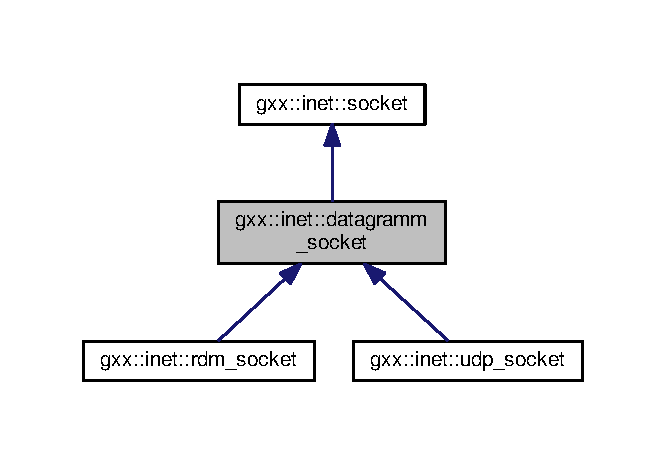
\includegraphics[width=320pt]{structgxx_1_1inet_1_1datagramm__socket__inherit__graph}
\end{center}
\end{figure}


Collaboration diagram for gxx\+:\+:inet\+:\+:datagramm\+\_\+socket\+:
\nopagebreak
\begin{figure}[H]
\begin{center}
\leavevmode
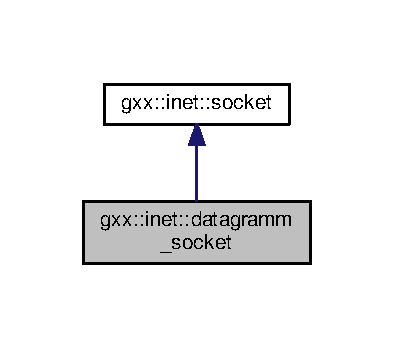
\includegraphics[width=189pt]{structgxx_1_1inet_1_1datagramm__socket__coll__graph}
\end{center}
\end{figure}
\subsection*{Public Member Functions}
\begin{DoxyCompactItemize}
\item 
{\bfseries datagramm\+\_\+socket} (int domain, int type, int proto)\hypertarget{structgxx_1_1inet_1_1datagramm__socket_a9439e5f734cec85e17b1b2f4bf1db4d1}{}\label{structgxx_1_1inet_1_1datagramm__socket_a9439e5f734cec85e17b1b2f4bf1db4d1}

\item 
int {\bfseries sendto} (\hyperlink{classgxx_1_1hostaddr}{gxx\+::inet\+::hostaddr} haddr, int port, const char $\ast$data, size\+\_\+t size)\hypertarget{structgxx_1_1inet_1_1datagramm__socket_a28e77b93fd7040079e4cb9353ad263b3}{}\label{structgxx_1_1inet_1_1datagramm__socket_a28e77b93fd7040079e4cb9353ad263b3}

\item 
int {\bfseries recvfrom} (char $\ast$data, size\+\_\+t maxsize, \hyperlink{structgxx_1_1inet_1_1netaddr}{gxx\+::inet\+::netaddr} $\ast$inaddr)\hypertarget{structgxx_1_1inet_1_1datagramm__socket_a8459652652779265adac1180afb12749}{}\label{structgxx_1_1inet_1_1datagramm__socket_a8459652652779265adac1180afb12749}

\end{DoxyCompactItemize}
\subsection*{Additional Inherited Members}


The documentation for this struct was generated from the following files\+:\begin{DoxyCompactItemize}
\item 
/home/rfmeas/project/gxx/gxx/inet/dgramm.\+h\item 
/home/rfmeas/project/gxx/gxx/inet/src/common.\+cpp\end{DoxyCompactItemize}

\hypertarget{structgxx_1_1time_1_1datetime}{}\section{gxx\+:\+:time\+:\+:datetime Struct Reference}
\label{structgxx_1_1time_1_1datetime}\index{gxx\+::time\+::datetime@{gxx\+::time\+::datetime}}
\subsection*{Public Attributes}
\begin{DoxyCompactItemize}
\item 
std\+::tm {\bfseries native}\hypertarget{structgxx_1_1time_1_1datetime_a29a778f2d392426b7478dcfe00ca5b07}{}\label{structgxx_1_1time_1_1datetime_a29a778f2d392426b7478dcfe00ca5b07}

\end{DoxyCompactItemize}


The documentation for this struct was generated from the following file\+:\begin{DoxyCompactItemize}
\item 
/home/rfmeas/project/gxx/gxx/time/datetime.\+h\end{DoxyCompactItemize}

\hypertarget{classgxx_1_1debug__ostream}{}\section{gxx\+:\+:debug\+\_\+ostream Class Reference}
\label{classgxx_1_1debug__ostream}\index{gxx\+::debug\+\_\+ostream@{gxx\+::debug\+\_\+ostream}}


Inheritance diagram for gxx\+:\+:debug\+\_\+ostream\+:
% FIG 0


Collaboration diagram for gxx\+:\+:debug\+\_\+ostream\+:
% FIG 1
\subsection*{Public Member Functions}
\begin{DoxyCompactItemize}
\item 
{\bfseries A\+C\+C\+E\+S\+S\+OR} (hexmode, \+\_\+hexmode)\hypertarget{classgxx_1_1debug__ostream_a26f05c9a368bfa5fbfaf429793f1b852}{}\label{classgxx_1_1debug__ostream_a26f05c9a368bfa5fbfaf429793f1b852}

\item 
int {\bfseries write} (const char $\ast$str, size\+\_\+t sz) override\hypertarget{classgxx_1_1debug__ostream_af320da6e96d352b36e69cdf9ad5a066c}{}\label{classgxx_1_1debug__ostream_af320da6e96d352b36e69cdf9ad5a066c}

\item 
int {\bfseries putchar} (const char c) override\hypertarget{classgxx_1_1debug__ostream_abc694d8fbedd07135143cdd068aae343}{}\label{classgxx_1_1debug__ostream_abc694d8fbedd07135143cdd068aae343}

\end{DoxyCompactItemize}
\subsection*{Protected Member Functions}
\begin{DoxyCompactItemize}
\item 
int {\bfseries write\+Data} (const char $\ast$data, size\+\_\+t max\+Size)\hypertarget{classgxx_1_1debug__ostream_ab0d598e63b09f75a583a9212394ade79}{}\label{classgxx_1_1debug__ostream_ab0d598e63b09f75a583a9212394ade79}

\end{DoxyCompactItemize}


The documentation for this class was generated from the following files\+:\begin{DoxyCompactItemize}
\item 
/home/rfmeas/project/gxx/gxx/debug/debug\+\_\+ostream.\+h\item 
/home/rfmeas/project/gxx/gxx/\+H\+I\+D\+E/io/iostream.\+h\end{DoxyCompactItemize}

\hypertarget{classgxx_1_1io_1_1debug__ostream}{}\section{gxx\+:\+:io\+:\+:debug\+\_\+ostream Class Reference}
\label{classgxx_1_1io_1_1debug__ostream}\index{gxx\+::io\+::debug\+\_\+ostream@{gxx\+::io\+::debug\+\_\+ostream}}


Inheritance diagram for gxx\+:\+:io\+:\+:debug\+\_\+ostream\+:
% FIG 0


Collaboration diagram for gxx\+:\+:io\+:\+:debug\+\_\+ostream\+:
% FIG 1


The documentation for this class was generated from the following file\+:\begin{DoxyCompactItemize}
\item 
/home/rfmeas/project/gxx/gxx/io/\+H\+I\+D\+E/debug\+\_\+ostream.\+h\end{DoxyCompactItemize}

\hypertarget{classgxx_1_1io_1_1debug__streambuf}{}\section{gxx\+:\+:io\+:\+:debug\+\_\+streambuf Class Reference}
\label{classgxx_1_1io_1_1debug__streambuf}\index{gxx\+::io\+::debug\+\_\+streambuf@{gxx\+::io\+::debug\+\_\+streambuf}}


Inheritance diagram for gxx\+:\+:io\+:\+:debug\+\_\+streambuf\+:
\nopagebreak
\begin{figure}[H]
\begin{center}
\leavevmode
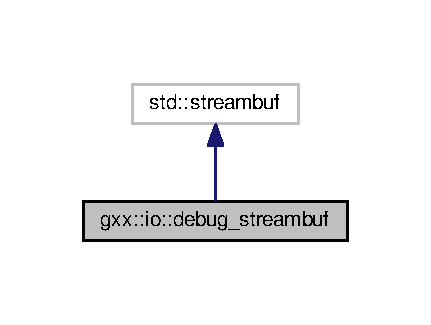
\includegraphics[width=207pt]{classgxx_1_1io_1_1debug__streambuf__inherit__graph}
\end{center}
\end{figure}


Collaboration diagram for gxx\+:\+:io\+:\+:debug\+\_\+streambuf\+:
\nopagebreak
\begin{figure}[H]
\begin{center}
\leavevmode
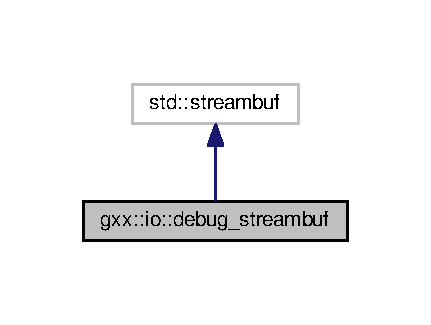
\includegraphics[width=207pt]{classgxx_1_1io_1_1debug__streambuf__coll__graph}
\end{center}
\end{figure}


The documentation for this class was generated from the following file\+:\begin{DoxyCompactItemize}
\item 
/home/rfmeas/project/gxx/gxx/io/\+H\+I\+D\+E/debug\+\_\+ostream.\+h\end{DoxyCompactItemize}

\hypertarget{classgxx_1_1io_1_1debug__strmout}{}\section{gxx\+:\+:io\+:\+:debug\+\_\+strmout Class Reference}
\label{classgxx_1_1io_1_1debug__strmout}\index{gxx\+::io\+::debug\+\_\+strmout@{gxx\+::io\+::debug\+\_\+strmout}}


Inheritance diagram for gxx\+:\+:io\+:\+:debug\+\_\+strmout\+:
% FIG 0


Collaboration diagram for gxx\+:\+:io\+:\+:debug\+\_\+strmout\+:
% FIG 1
\subsection*{Public Member Functions}
\begin{DoxyCompactItemize}
\item 
int {\bfseries write\+Data} (const char $\ast$str, size\+\_\+t sz) override\hypertarget{classgxx_1_1io_1_1debug__strmout_adb8926ce207b7d278a82f63cfe3c7a83}{}\label{classgxx_1_1io_1_1debug__strmout_adb8926ce207b7d278a82f63cfe3c7a83}

\item 
int {\bfseries putchar} (const char c) override\hypertarget{classgxx_1_1io_1_1debug__strmout_a5a86485ab4721b21b9e7e7cc25784dfc}{}\label{classgxx_1_1io_1_1debug__strmout_a5a86485ab4721b21b9e7e7cc25784dfc}

\item 
void {\bfseries dumpmode} (bool en)\hypertarget{classgxx_1_1io_1_1debug__strmout_a61b908e1b1b31c3356d9a152bb1b7eda}{}\label{classgxx_1_1io_1_1debug__strmout_a61b908e1b1b31c3356d9a152bb1b7eda}

\item 
int {\bfseries write\+Data} (const char $\ast$str, size\+\_\+t sz) override\hypertarget{classgxx_1_1io_1_1debug__strmout_adb8926ce207b7d278a82f63cfe3c7a83}{}\label{classgxx_1_1io_1_1debug__strmout_adb8926ce207b7d278a82f63cfe3c7a83}

\item 
int {\bfseries putchar} (const char c) override\hypertarget{classgxx_1_1io_1_1debug__strmout_a5a86485ab4721b21b9e7e7cc25784dfc}{}\label{classgxx_1_1io_1_1debug__strmout_a5a86485ab4721b21b9e7e7cc25784dfc}

\item 
void {\bfseries dumpmode} (bool en)\hypertarget{classgxx_1_1io_1_1debug__strmout_a61b908e1b1b31c3356d9a152bb1b7eda}{}\label{classgxx_1_1io_1_1debug__strmout_a61b908e1b1b31c3356d9a152bb1b7eda}

\item 
int {\bfseries write\+Data} (const char $\ast$str, size\+\_\+t sz) override\hypertarget{classgxx_1_1io_1_1debug__strmout_adb8926ce207b7d278a82f63cfe3c7a83}{}\label{classgxx_1_1io_1_1debug__strmout_adb8926ce207b7d278a82f63cfe3c7a83}

\item 
int {\bfseries putchar} (const char c) override\hypertarget{classgxx_1_1io_1_1debug__strmout_a5a86485ab4721b21b9e7e7cc25784dfc}{}\label{classgxx_1_1io_1_1debug__strmout_a5a86485ab4721b21b9e7e7cc25784dfc}

\item 
void {\bfseries dumpmode} (bool en)\hypertarget{classgxx_1_1io_1_1debug__strmout_a61b908e1b1b31c3356d9a152bb1b7eda}{}\label{classgxx_1_1io_1_1debug__strmout_a61b908e1b1b31c3356d9a152bb1b7eda}

\end{DoxyCompactItemize}
\subsection*{Additional Inherited Members}


The documentation for this class was generated from the following file\+:\begin{DoxyCompactItemize}
\item 
/home/rfmeas/project/gxx/gxx/\+H\+I\+D\+E/ionew/strm.\+h\end{DoxyCompactItemize}

\hypertarget{structdecay}{}\section{decay$<$ T $>$ Struct Template Reference}
\label{structdecay}\index{decay$<$ T $>$@{decay$<$ T $>$}}
\subsection*{Public Types}
\begin{DoxyCompactItemize}
\item 
typedef gxx\+::conditional$<$ gxx\+::is\+\_\+array$<$ U $>$\+::value, typename gxx\+::remove\+\_\+extent$<$ U $>$\+::type $\ast$, typename gxx\+::conditional$<$ gxx\+::is\+\_\+function$<$ U $>$\+::value, typename gxx\+::add\+\_\+pointer$<$ U $>$\+::type, typename gxx\+::remove\+\_\+cv$<$ U $>$\+::type $>$\+::type $>$\+::type {\bfseries type}\hypertarget{structdecay_a4fdf85f3a145ca2be69b59a1dba61139}{}\label{structdecay_a4fdf85f3a145ca2be69b59a1dba61139}

\item 
typedef std\+::conditional$<$ std\+::is\+\_\+array$<$ U $>$\+::value, typename std\+::remove\+\_\+extent$<$ U $>$\+::type $\ast$, typename std\+::conditional$<$ std\+::is\+\_\+function$<$ U $>$\+::value, typename std\+::add\+\_\+pointer$<$ U $>$\+::type, typename std\+::remove\+\_\+cv$<$ U $>$\+::type $>$\+::type $>$\+::type {\bfseries type}\hypertarget{structdecay_ae011f354b41d8e173094d454939a1b5a}{}\label{structdecay_ae011f354b41d8e173094d454939a1b5a}

\end{DoxyCompactItemize}


The documentation for this struct was generated from the following file\+:\begin{DoxyCompactItemize}
\item 
/home/rfmeas/project/gxx/gxx/\+H\+I\+D\+E/utility/type\+\_\+relation.\+hpp\end{DoxyCompactItemize}

\hypertarget{classgxx_1_1default__deleter}{}\section{gxx\+:\+:default\+\_\+deleter$<$ T $>$ Class Template Reference}
\label{classgxx_1_1default__deleter}\index{gxx\+::default\+\_\+deleter$<$ T $>$@{gxx\+::default\+\_\+deleter$<$ T $>$}}
\subsection*{Public Member Functions}
\begin{DoxyCompactItemize}
\item 
void {\bfseries operator()} (T $\ast$ptr)\hypertarget{classgxx_1_1default__deleter_a0a94c817d8fb40eb33bb123d88022870}{}\label{classgxx_1_1default__deleter_a0a94c817d8fb40eb33bb123d88022870}

\end{DoxyCompactItemize}


The documentation for this class was generated from the following file\+:\begin{DoxyCompactItemize}
\item 
/home/rfmeas/project/gxx/gxx/\+H\+I\+D\+E/shared.\+h\end{DoxyCompactItemize}

\hypertarget{classgxx_1_1deffered}{}\section{gxx\+:\+:deffered$<$ Ret, Args $>$ Class Template Reference}
\label{classgxx_1_1deffered}\index{gxx\+::deffered$<$ Ret, Args $>$@{gxx\+::deffered$<$ Ret, Args $>$}}


Collaboration diagram for gxx\+:\+:deffered$<$ Ret, Args $>$\+:
\nopagebreak
\begin{figure}[H]
\begin{center}
\leavevmode
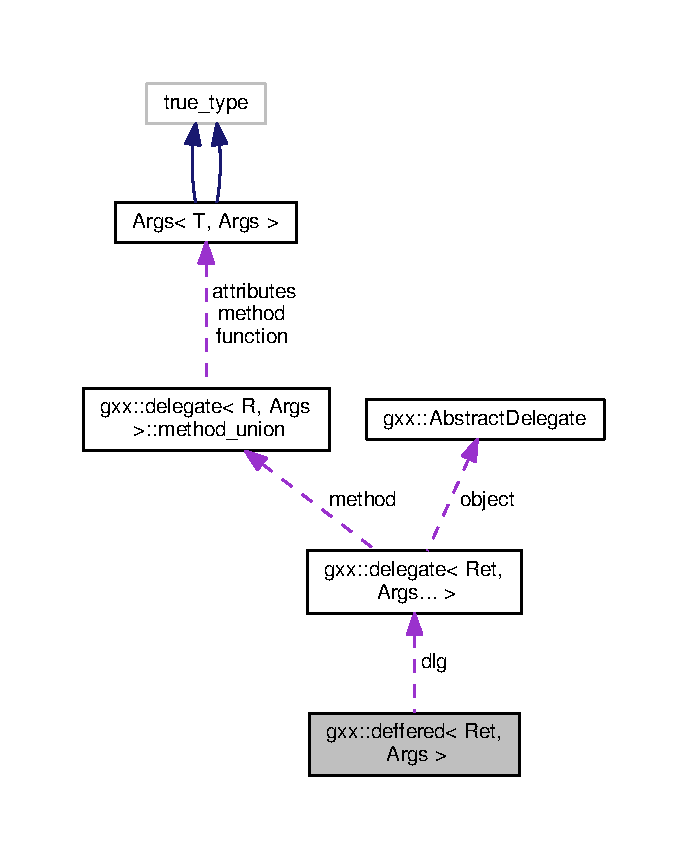
\includegraphics[width=330pt]{classgxx_1_1deffered__coll__graph}
\end{center}
\end{figure}
\subsection*{Public Member Functions}
\begin{DoxyCompactItemize}
\item 
{\footnotesize template$<$typename... U\+Args$>$ }\\{\bfseries deffered} (const \hyperlink{classgxx_1_1delegate}{gxx\+::delegate}$<$ Ret, Args... $>$ \&dlg, U\+Args...\+args)\hypertarget{classgxx_1_1deffered_ab813cdb2f51d78d695c1f4f807225d59}{}\label{classgxx_1_1deffered_ab813cdb2f51d78d695c1f4f807225d59}

\item 
Ret {\bfseries invoke} ()\hypertarget{classgxx_1_1deffered_a1bea81d7b89cf185a4e465589d2f7744}{}\label{classgxx_1_1deffered_a1bea81d7b89cf185a4e465589d2f7744}

\end{DoxyCompactItemize}
\subsection*{Public Attributes}
\begin{DoxyCompactItemize}
\item 
\hyperlink{classgxx_1_1delegate}{gxx\+::delegate}$<$ Ret, Args... $>$ {\bfseries dlg}\hypertarget{classgxx_1_1deffered_ae53c058c74221d95cef72d4d49732603}{}\label{classgxx_1_1deffered_ae53c058c74221d95cef72d4d49732603}

\item 
std\+::tuple$<$ Args... $>$ {\bfseries args}\hypertarget{classgxx_1_1deffered_ae9951bf8d9eb1baca9b9da699f068fc5}{}\label{classgxx_1_1deffered_ae9951bf8d9eb1baca9b9da699f068fc5}

\end{DoxyCompactItemize}


The documentation for this class was generated from the following file\+:\begin{DoxyCompactItemize}
\item 
/home/rfmeas/project/gxx/gxx/event/deffered.\+h\end{DoxyCompactItemize}

\hypertarget{classgxx_1_1delegate}{}\section{gxx\+:\+:delegate$<$ R, Args $>$ Class Template Reference}
\label{classgxx_1_1delegate}\index{gxx\+::delegate$<$ R, Args $>$@{gxx\+::delegate$<$ R, Args $>$}}


Collaboration diagram for gxx\+:\+:delegate$<$ R, Args $>$\+:
\nopagebreak
\begin{figure}[H]
\begin{center}
\leavevmode
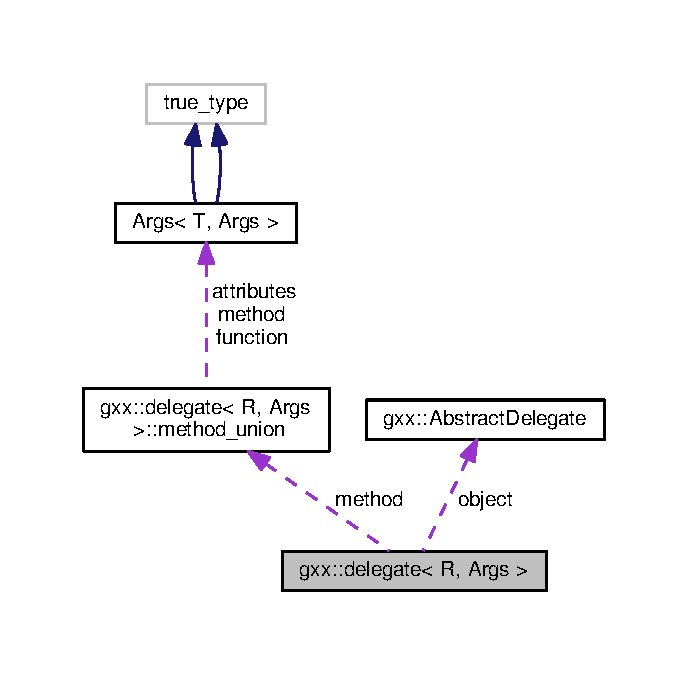
\includegraphics[width=330pt]{classgxx_1_1delegate__coll__graph}
\end{center}
\end{figure}
\subsection*{Classes}
\begin{DoxyCompactItemize}
\item 
union \hyperlink{uniongxx_1_1delegate_1_1method__union}{method\+\_\+union}
\end{DoxyCompactItemize}
\subsection*{Public Member Functions}
\begin{DoxyCompactItemize}
\item 
void {\bfseries clean} ()\hypertarget{classgxx_1_1delegate_a05d3145f26fb4746cf9a6b3a66878e2b}{}\label{classgxx_1_1delegate_a05d3145f26fb4746cf9a6b3a66878e2b}

\item 
bool {\bfseries armed} ()\hypertarget{classgxx_1_1delegate_aa099acfe63f6020c9b10fd0a4a66dd38}{}\label{classgxx_1_1delegate_aa099acfe63f6020c9b10fd0a4a66dd38}

\item 
{\bfseries delegate} (const \hyperlink{classgxx_1_1delegate}{delegate} \&d)\hypertarget{classgxx_1_1delegate_aeda82a43206c3c085eb6eeb886520eac}{}\label{classgxx_1_1delegate_aeda82a43206c3c085eb6eeb886520eac}

\item 
{\bfseries delegate} (\hyperlink{classgxx_1_1delegate}{delegate} \&\&d)\hypertarget{classgxx_1_1delegate_a6620927526106282562e9adabe6ed41e}{}\label{classgxx_1_1delegate_a6620927526106282562e9adabe6ed41e}

\item 
{\bfseries delegate} (const fnc\+\_\+t func)\hypertarget{classgxx_1_1delegate_a4af7c79563f2d8904aa47cb2356270f5}{}\label{classgxx_1_1delegate_a4af7c79563f2d8904aa47cb2356270f5}

\item 
{\footnotesize template$<$typename T $>$ }\\{\bfseries delegate} (R(T\+::$\ast$mtd)(Args...), T $\ast$ptr\+\_\+obj)\hypertarget{classgxx_1_1delegate_ada0fc8f4b45e96e1cc7005975f136bc9}{}\label{classgxx_1_1delegate_ada0fc8f4b45e96e1cc7005975f136bc9}

\item 
{\footnotesize template$<$typename F $>$ }\\{\bfseries delegate} (const F \&functor)\hypertarget{classgxx_1_1delegate_a2cfc41012504d91f7f8e69d297c75f3b}{}\label{classgxx_1_1delegate_a2cfc41012504d91f7f8e69d297c75f3b}

\item 
\hyperlink{classgxx_1_1delegate}{delegate} \& {\bfseries operator=} (const \hyperlink{classgxx_1_1delegate}{delegate} \&d)\hypertarget{classgxx_1_1delegate_af6cc59c9a81f36da06aceead7dd0b6e5}{}\label{classgxx_1_1delegate_af6cc59c9a81f36da06aceead7dd0b6e5}

\item 
\hyperlink{classgxx_1_1delegate}{delegate} \& {\bfseries operator=} (\hyperlink{classgxx_1_1delegate}{delegate} \&\&d)\hypertarget{classgxx_1_1delegate_a942965b72aa98b564f3b9fcc5e2769e4}{}\label{classgxx_1_1delegate_a942965b72aa98b564f3b9fcc5e2769e4}

\item 
R {\bfseries operator()} (Args...\+arg)\hypertarget{classgxx_1_1delegate_a62c64d47078a90986be2920ef6d2aa8f}{}\label{classgxx_1_1delegate_a62c64d47078a90986be2920ef6d2aa8f}

\item 
bool {\bfseries operator==} (\hyperlink{classgxx_1_1delegate}{delegate}$<$ R, Args... $>$ b)\hypertarget{classgxx_1_1delegate_a9a726537a2dbaa5f922dee3e76b464a0}{}\label{classgxx_1_1delegate_a9a726537a2dbaa5f922dee3e76b464a0}

\item 
R {\bfseries emit\+\_\+and\+\_\+reset} (Args...\+args)\hypertarget{classgxx_1_1delegate_a309788f98a8dd4554790550b373b3116}{}\label{classgxx_1_1delegate_a309788f98a8dd4554790550b373b3116}

\end{DoxyCompactItemize}
\subsection*{Protected Types}
\begin{DoxyCompactItemize}
\item 
enum \{ {\bfseries M\+E\+T\+H\+OD}, 
{\bfseries F\+U\+N\+C\+T\+I\+ON}
 \}\hypertarget{classgxx_1_1delegate_a554a52c49e319312eea93ccd8aa118a3}{}\label{classgxx_1_1delegate_a554a52c49e319312eea93ccd8aa118a3}

\item 
using {\bfseries obj\+\_\+t} = \hyperlink{classgxx_1_1AbstractDelegate}{Abstract\+Delegate} $\ast$\hypertarget{classgxx_1_1delegate_a6b84dc0b374f80cb03c0290403cd7f78}{}\label{classgxx_1_1delegate_a6b84dc0b374f80cb03c0290403cd7f78}

\item 
using {\bfseries mtd\+\_\+t} = R(Abstract\+Delegate\+::$\ast$)(Args...)\hypertarget{classgxx_1_1delegate_a4995c00b9f75767b129a153b6f982d4b}{}\label{classgxx_1_1delegate_a4995c00b9f75767b129a153b6f982d4b}

\item 
using {\bfseries fnc\+\_\+t} = R($\ast$)(Args...)\hypertarget{classgxx_1_1delegate_aa15443cd7b3f360edf6672e69d61718b}{}\label{classgxx_1_1delegate_aa15443cd7b3f360edf6672e69d61718b}

\item 
using {\bfseries extfnc\+\_\+t} = R($\ast$)(void $\ast$,Args...)\hypertarget{classgxx_1_1delegate_ab4ad330d6c5142761478dade9aeeae2b}{}\label{classgxx_1_1delegate_ab4ad330d6c5142761478dade9aeeae2b}

\item 
using {\bfseries absmemb\+\_\+t} = std\+::pair$<$ mtd\+\_\+t, \hyperlink{classgxx_1_1AbstractDelegate}{obj\+\_\+t} $>$\hypertarget{classgxx_1_1delegate_ab5c94c447daf8c6b1f539fcbdb413a99}{}\label{classgxx_1_1delegate_ab5c94c447daf8c6b1f539fcbdb413a99}

\end{DoxyCompactItemize}
\subsection*{Protected Attributes}
\begin{DoxyCompactItemize}
\item 
\hyperlink{classgxx_1_1AbstractDelegate}{obj\+\_\+t} {\bfseries object}\hypertarget{classgxx_1_1delegate_a4f01586b3720f0cdc4b50e6f8cedb08e}{}\label{classgxx_1_1delegate_a4f01586b3720f0cdc4b50e6f8cedb08e}

\item 
\hyperlink{uniongxx_1_1delegate_1_1method__union}{method\+\_\+union} {\bfseries method}\hypertarget{classgxx_1_1delegate_aae23f8e6e23ca3a5d8d764932e376ea0}{}\label{classgxx_1_1delegate_aae23f8e6e23ca3a5d8d764932e376ea0}

\end{DoxyCompactItemize}


The documentation for this class was generated from the following file\+:\begin{DoxyCompactItemize}
\item 
/home/rfmeas/project/gxx/gxx/event/delegate.\+h\end{DoxyCompactItemize}

\hypertarget{classgxx_1_1io_1_1dgrammer}{}\section{gxx\+:\+:io\+:\+:dgrammer Class Reference}
\label{classgxx_1_1io_1_1dgrammer}\index{gxx\+::io\+::dgrammer@{gxx\+::io\+::dgrammer}}


The documentation for this class was generated from the following file\+:\begin{DoxyCompactItemize}
\item 
/home/rfmeas/project/gxx/gxx/io/dgramm.\+h\end{DoxyCompactItemize}

\hypertarget{structdiag__ops}{}\section{diag\+\_\+ops Struct Reference}
\label{structdiag__ops}\index{diag\+\_\+ops@{diag\+\_\+ops}}
\subsection*{Public Attributes}
\begin{DoxyCompactItemize}
\item 
int($\ast$ {\bfseries putc} )(void $\ast$, char)\hypertarget{structdiag__ops_a7d2d9c74bfc6c7993185ed57bfd6904e}{}\label{structdiag__ops_a7d2d9c74bfc6c7993185ed57bfd6904e}

\item 
int($\ast$ {\bfseries getc} )(void $\ast$)\hypertarget{structdiag__ops_a300331d1c1fb543e26cf6cfa53a26a66}{}\label{structdiag__ops_a300331d1c1fb543e26cf6cfa53a26a66}

\item 
int($\ast$ {\bfseries write} )(void $\ast$, const char $\ast$, int)\hypertarget{structdiag__ops_a45c3b44ce406c21aa0c88250735635da}{}\label{structdiag__ops_a45c3b44ce406c21aa0c88250735635da}

\item 
int($\ast$ {\bfseries read} )(void $\ast$, char $\ast$, int)\hypertarget{structdiag__ops_acc346736df0c59676a8c8646d6111dc4}{}\label{structdiag__ops_acc346736df0c59676a8c8646d6111dc4}

\end{DoxyCompactItemize}


The documentation for this struct was generated from the following file\+:\begin{DoxyCompactItemize}
\item 
/home/rfmeas/project/gxx/gxx/diag/diag.\+h\end{DoxyCompactItemize}

\hypertarget{structgxx_1_1schema_1_1dict}{}\section{gxx\+:\+:schema\+:\+:dict Struct Reference}
\label{structgxx_1_1schema_1_1dict}\index{gxx\+::schema\+::dict@{gxx\+::schema\+::dict}}


Inheritance diagram for gxx\+:\+:schema\+:\+:dict\+:
% FIG 0


Collaboration diagram for gxx\+:\+:schema\+:\+:dict\+:
% FIG 1
\subsection*{Public Member Functions}
\begin{DoxyCompactItemize}
\item 
{\bfseries dict} (const std\+::initializer\+\_\+list$<$ \hyperlink{structgxx_1_1schema_1_1schema__dict__pair}{schema\+\_\+dict\+\_\+pair} $>$ \&lst)\hypertarget{structgxx_1_1schema_1_1dict_adde30152a288ea3a1f60426caa50f27b}{}\label{structgxx_1_1schema_1_1dict_adde30152a288ea3a1f60426caa50f27b}

\end{DoxyCompactItemize}
\subsection*{Additional Inherited Members}


The documentation for this struct was generated from the following file\+:\begin{DoxyCompactItemize}
\item 
/home/rfmeas/project/gxx/gxx/trent/schema.\+h\end{DoxyCompactItemize}

\hypertarget{structgxx_1_1math_1_1directed__interval}{}\section{gxx\+:\+:math\+:\+:directed\+\_\+interval$<$ T $>$ Struct Template Reference}
\label{structgxx_1_1math_1_1directed__interval}\index{gxx\+::math\+::directed\+\_\+interval$<$ T $>$@{gxx\+::math\+::directed\+\_\+interval$<$ T $>$}}


Inheritance diagram for gxx\+:\+:math\+:\+:directed\+\_\+interval$<$ T $>$\+:
\nopagebreak
\begin{figure}[H]
\begin{center}
\leavevmode
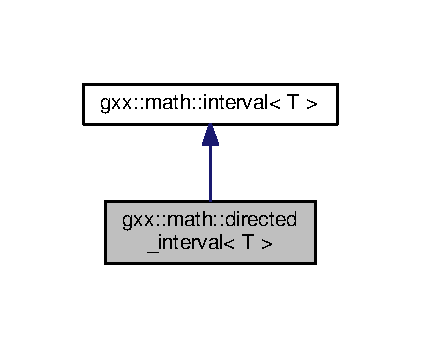
\includegraphics[width=202pt]{structgxx_1_1math_1_1directed__interval__inherit__graph}
\end{center}
\end{figure}


Collaboration diagram for gxx\+:\+:math\+:\+:directed\+\_\+interval$<$ T $>$\+:
\nopagebreak
\begin{figure}[H]
\begin{center}
\leavevmode
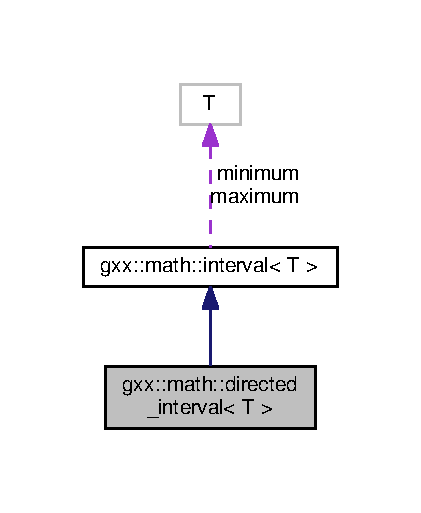
\includegraphics[width=202pt]{structgxx_1_1math_1_1directed__interval__coll__graph}
\end{center}
\end{figure}
\subsection*{Public Member Functions}
\begin{DoxyCompactItemize}
\item 
{\bfseries directed\+\_\+interval} (T strt, T stop)\hypertarget{structgxx_1_1math_1_1directed__interval_a56c727a9876226b8323eef2ec8f467f2}{}\label{structgxx_1_1math_1_1directed__interval_a56c727a9876226b8323eef2ec8f467f2}

\item 
T {\bfseries start} () const \hypertarget{structgxx_1_1math_1_1directed__interval_a4a7f41f73a08e7d79ab7a4dd1b040e2d}{}\label{structgxx_1_1math_1_1directed__interval_a4a7f41f73a08e7d79ab7a4dd1b040e2d}

\item 
T {\bfseries finish} () const \hypertarget{structgxx_1_1math_1_1directed__interval_aa966173ddac24be355e4da10fce0d187}{}\label{structgxx_1_1math_1_1directed__interval_aa966173ddac24be355e4da10fce0d187}

\item 
T {\bfseries proc} (double prc) const \hypertarget{structgxx_1_1math_1_1directed__interval_ae816022ac342134d35d5af4c200f0748}{}\label{structgxx_1_1math_1_1directed__interval_ae816022ac342134d35d5af4c200f0748}

\item 
double {\bfseries to\+\_\+proc} (T param) const \hypertarget{structgxx_1_1math_1_1directed__interval_ac74ae93897c07b766cba868777d5f686}{}\label{structgxx_1_1math_1_1directed__interval_ac74ae93897c07b766cba868777d5f686}

\end{DoxyCompactItemize}
\subsection*{Public Attributes}
\begin{DoxyCompactItemize}
\item 
bool {\bfseries reverse}\hypertarget{structgxx_1_1math_1_1directed__interval_a54217a3c25abb1c06c23505cac30fdfd}{}\label{structgxx_1_1math_1_1directed__interval_a54217a3c25abb1c06c23505cac30fdfd}

\end{DoxyCompactItemize}


The documentation for this struct was generated from the following file\+:\begin{DoxyCompactItemize}
\item 
/home/rfmeas/project/gxx/gxx/math/interval.\+h\end{DoxyCompactItemize}

\hypertarget{classgxx_1_1geom3_1_1direction}{}\section{gxx\+:\+:geom3\+:\+:direction Class Reference}
\label{classgxx_1_1geom3_1_1direction}\index{gxx\+::geom3\+::direction@{gxx\+::geom3\+::direction}}


Inheritance diagram for gxx\+:\+:geom3\+:\+:direction\+:
\nopagebreak
\begin{figure}[H]
\begin{center}
\leavevmode
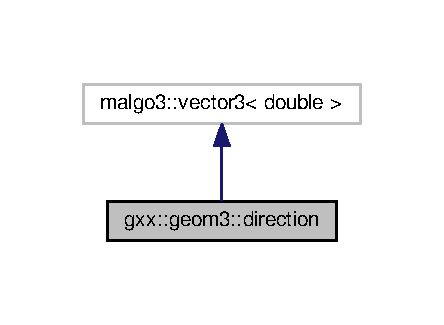
\includegraphics[width=213pt]{classgxx_1_1geom3_1_1direction__inherit__graph}
\end{center}
\end{figure}


Collaboration diagram for gxx\+:\+:geom3\+:\+:direction\+:
\nopagebreak
\begin{figure}[H]
\begin{center}
\leavevmode
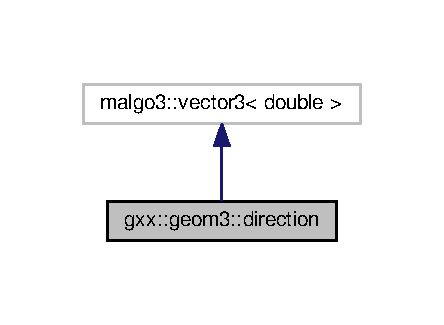
\includegraphics[width=213pt]{classgxx_1_1geom3_1_1direction__coll__graph}
\end{center}
\end{figure}
\subsection*{Public Member Functions}
\begin{DoxyCompactItemize}
\item 
{\bfseries direction} (double x, double y, double z, bool norm=true)\hypertarget{classgxx_1_1geom3_1_1direction_a6358587d647d516db1083f64e1fd68da}{}\label{classgxx_1_1geom3_1_1direction_a6358587d647d516db1083f64e1fd68da}

\item 
{\bfseries direction} (const \hyperlink{classgxx_1_1geom3_1_1direction}{direction} \&oth)\hypertarget{classgxx_1_1geom3_1_1direction_ad1915bd7cbea2e42ad61bb1e5362691e}{}\label{classgxx_1_1geom3_1_1direction_ad1915bd7cbea2e42ad61bb1e5362691e}

\item 
{\bfseries direction} (const malgo3\+::vector3$<$ double $>$ \&oth, bool norm=true)\hypertarget{classgxx_1_1geom3_1_1direction_a431eb925ed7a72e7491d149da2b58ab9}{}\label{classgxx_1_1geom3_1_1direction_a431eb925ed7a72e7491d149da2b58ab9}

\end{DoxyCompactItemize}


The documentation for this class was generated from the following file\+:\begin{DoxyCompactItemize}
\item 
/home/rfmeas/project/gxx/gxx/geom/geom3.\+h\end{DoxyCompactItemize}

\hypertarget{classgxx_1_1ngeom_1_1direction}{}\section{gxx\+:\+:ngeom\+:\+:direction Class Reference}
\label{classgxx_1_1ngeom_1_1direction}\index{gxx\+::ngeom\+::direction@{gxx\+::ngeom\+::direction}}


Inheritance diagram for gxx\+:\+:ngeom\+:\+:direction\+:
\nopagebreak
\begin{figure}[H]
\begin{center}
\leavevmode
\includegraphics[width=204pt]{classgxx_1_1ngeom_1_1direction__inherit__graph}
\end{center}
\end{figure}


Collaboration diagram for gxx\+:\+:ngeom\+:\+:direction\+:
\nopagebreak
\begin{figure}[H]
\begin{center}
\leavevmode
\includegraphics[width=204pt]{classgxx_1_1ngeom_1_1direction__coll__graph}
\end{center}
\end{figure}
\subsection*{Public Member Functions}
\begin{DoxyCompactItemize}
\item 
{\bfseries direction} (\hyperlink{classgxx_1_1object__buffer}{gxx\+::objbuf}$<$ double $>$ buf)\hypertarget{classgxx_1_1ngeom_1_1direction_a27b9b59ef7e2f99c9555b051447530a3}{}\label{classgxx_1_1ngeom_1_1direction_a27b9b59ef7e2f99c9555b051447530a3}

\end{DoxyCompactItemize}
\subsection*{Additional Inherited Members}


The documentation for this class was generated from the following file\+:\begin{DoxyCompactItemize}
\item 
/home/rfmeas/project/gxx/gxx/geom/ngeom.\+h\end{DoxyCompactItemize}

\hypertarget{classgxx_1_1path_1_1directory}{}\section{gxx\+:\+:path\+:\+:directory Class Reference}
\label{classgxx_1_1path_1_1directory}\index{gxx\+::path\+::directory@{gxx\+::path\+::directory}}
\subsection*{Public Member Functions}
\begin{DoxyCompactItemize}
\item 
{\bfseries directory} (gxx\+::path pth)\hypertarget{classgxx_1_1path_1_1directory_aaabf4de76bdb600822314f86f1d93831}{}\label{classgxx_1_1path_1_1directory_aaabf4de76bdb600822314f86f1d93831}

\item 
bool {\bfseries exist} ()\hypertarget{classgxx_1_1path_1_1directory_a328c2d048fe528298dcb390ac0b8281d}{}\label{classgxx_1_1path_1_1directory_a328c2d048fe528298dcb390ac0b8281d}

\item 
bool {\bfseries make} ()\hypertarget{classgxx_1_1path_1_1directory_a263c2d67881dea992c915d223ab9c856}{}\label{classgxx_1_1path_1_1directory_a263c2d67881dea992c915d223ab9c856}

\item 
bool {\bfseries make\+\_\+recurse} ()\hypertarget{classgxx_1_1path_1_1directory_a6f3450d67583019ac3e382ebe3b050ad}{}\label{classgxx_1_1path_1_1directory_a6f3450d67583019ac3e382ebe3b050ad}

\end{DoxyCompactItemize}


The documentation for this class was generated from the following file\+:\begin{DoxyCompactItemize}
\item 
/home/rfmeas/project/gxx/gxx/path/directory.\+h\end{DoxyCompactItemize}

\hypertarget{classgxx_1_1unix_1_1directory}{}\section{gxx\+:\+:unix\+:\+:directory Class Reference}
\label{classgxx_1_1unix_1_1directory}\index{gxx\+::unix\+::directory@{gxx\+::unix\+::directory}}
\subsection*{Public Member Functions}
\begin{DoxyCompactItemize}
\item 
{\bfseries directory} (const char $\ast$path)\hypertarget{classgxx_1_1unix_1_1directory_a32ad84cf9bf95cc04b0b932656630311}{}\label{classgxx_1_1unix_1_1directory_a32ad84cf9bf95cc04b0b932656630311}

\item 
bool {\bfseries is\+\_\+exist} ()\hypertarget{classgxx_1_1unix_1_1directory_a3e36c1cf11dbf4468df302e1f1bbad57}{}\label{classgxx_1_1unix_1_1directory_a3e36c1cf11dbf4468df302e1f1bbad57}

\item 
\hyperlink{classgxx_1_1vector}{gxx\+::vector}$<$ \hyperlink{classgxx_1_1basic__string}{gxx\+::string} $>$ {\bfseries entry\+List} ()\hypertarget{classgxx_1_1unix_1_1directory_a626d2400492cf3a86ae417a047a12182}{}\label{classgxx_1_1unix_1_1directory_a626d2400492cf3a86ae417a047a12182}

\end{DoxyCompactItemize}


The documentation for this class was generated from the following file\+:\begin{DoxyCompactItemize}
\item 
/home/rfmeas/project/gxx/gxx/\+H\+I\+D\+E/io/unix/directory.\+h\end{DoxyCompactItemize}

\hypertarget{classgxx_1_1log_1_1directory__target}{}\section{gxx\+:\+:log\+:\+:directory\+\_\+target Class Reference}
\label{classgxx_1_1log_1_1directory__target}\index{gxx\+::log\+::directory\+\_\+target@{gxx\+::log\+::directory\+\_\+target}}


The documentation for this class was generated from the following file\+:\begin{DoxyCompactItemize}
\item 
/home/rfmeas/project/gxx/gxx/log/targets/directory\+\_\+target.\+h\end{DoxyCompactItemize}

\hypertarget{structlinalg_1_1op_1_1div}{}\section{linalg\+:\+:op\+:\+:div$<$ T $>$ Struct Template Reference}
\label{structlinalg_1_1op_1_1div}\index{linalg\+::op\+::div$<$ T $>$@{linalg\+::op\+::div$<$ T $>$}}
\subsection*{Public Member Functions}
\begin{DoxyCompactItemize}
\item 
constexpr auto {\bfseries operator()} (T l, T r) const -\/$>$ decltype(l/r)\hypertarget{structlinalg_1_1op_1_1div_ab1e9c67d78f78cb9c297bc88e7da4e36}{}\label{structlinalg_1_1op_1_1div_ab1e9c67d78f78cb9c297bc88e7da4e36}

\end{DoxyCompactItemize}


The documentation for this struct was generated from the following file\+:\begin{DoxyCompactItemize}
\item 
/home/rfmeas/project/gxx/gxx/math/linalg.\+h\end{DoxyCompactItemize}

\hypertarget{classgxx_1_1dlist}{}\section{gxx\+:\+:dlist$<$ type, member $>$ Class Template Reference}
\label{classgxx_1_1dlist}\index{gxx\+::dlist$<$ type, member $>$@{gxx\+::dlist$<$ type, member $>$}}


Collaboration diagram for gxx\+:\+:dlist$<$ type, member $>$\+:
\nopagebreak
\begin{figure}[H]
\begin{center}
\leavevmode
\includegraphics[width=218pt]{classgxx_1_1dlist__coll__graph}
\end{center}
\end{figure}
\subsection*{Classes}
\begin{DoxyCompactItemize}
\item 
class \hyperlink{classgxx_1_1dlist_1_1iterator}{iterator}
\item 
class \hyperlink{classgxx_1_1dlist_1_1reverse__iterator}{reverse\+\_\+iterator}
\end{DoxyCompactItemize}
\subsection*{Public Member Functions}
\begin{DoxyCompactItemize}
\item 
bool {\bfseries empty} ()\hypertarget{classgxx_1_1dlist_a73a909024bde20ad7e505c4bccfe6b35}{}\label{classgxx_1_1dlist_a73a909024bde20ad7e505c4bccfe6b35}

\item 
void {\bfseries move\+\_\+front} (type \&obj)\hypertarget{classgxx_1_1dlist_a83c8c62fd74a1ced6220728883209579}{}\label{classgxx_1_1dlist_a83c8c62fd74a1ced6220728883209579}

\item 
void {\bfseries move\+\_\+back} (type \&obj)\hypertarget{classgxx_1_1dlist_afa913fb0aa1cb04dfd47dc6ef2972193}{}\label{classgxx_1_1dlist_afa913fb0aa1cb04dfd47dc6ef2972193}

\item 
void {\bfseries move\+\_\+next} (type \&obj, type \&head)\hypertarget{classgxx_1_1dlist_a125345d98846237a75e517a865b680db}{}\label{classgxx_1_1dlist_a125345d98846237a75e517a865b680db}

\item 
void {\bfseries move\+\_\+next} (type \&obj, \hyperlink{classgxx_1_1dlist_1_1iterator}{iterator} head)\hypertarget{classgxx_1_1dlist_a0510d98090a688d7a60bb1522f0a2e9e}{}\label{classgxx_1_1dlist_a0510d98090a688d7a60bb1522f0a2e9e}

\item 
void {\bfseries move\+\_\+prev} (type \&obj, type \&head)\hypertarget{classgxx_1_1dlist_a182cd64f52ffda131a53a24cd0eac1a9}{}\label{classgxx_1_1dlist_a182cd64f52ffda131a53a24cd0eac1a9}

\item 
void {\bfseries move\+\_\+prev} (type \&obj, \hyperlink{classgxx_1_1dlist_1_1iterator}{iterator} head)\hypertarget{classgxx_1_1dlist_a207501ebd24f81980286311080095c80}{}\label{classgxx_1_1dlist_a207501ebd24f81980286311080095c80}

\item 
void {\bfseries pop} (type \&obj)\hypertarget{classgxx_1_1dlist_a93f5fc340642c0e0e638a20c65c13633}{}\label{classgxx_1_1dlist_a93f5fc340642c0e0e638a20c65c13633}

\item 
void {\bfseries del\+\_\+init} (type \&obj)\hypertarget{classgxx_1_1dlist_a7dc34a0db5bf47bb7f61679af2355139}{}\label{classgxx_1_1dlist_a7dc34a0db5bf47bb7f61679af2355139}

\item 
void {\bfseries pop\+\_\+if\+\_\+linked} (type \&obj)\hypertarget{classgxx_1_1dlist_adce409a635eecbb4d60a7ccffe4e43de}{}\label{classgxx_1_1dlist_adce409a635eecbb4d60a7ccffe4e43de}

\item 
void {\bfseries pop\+\_\+front} ()\hypertarget{classgxx_1_1dlist_a28f24370a924a70f6ad4f4ac048785c2}{}\label{classgxx_1_1dlist_a28f24370a924a70f6ad4f4ac048785c2}

\item 
void {\bfseries pop\+\_\+back} ()\hypertarget{classgxx_1_1dlist_a7977014927b96c831293e529972b1a7d}{}\label{classgxx_1_1dlist_a7977014927b96c831293e529972b1a7d}

\item 
void {\bfseries round\+\_\+left} ()\hypertarget{classgxx_1_1dlist_afb696fd066f87d89e8106921eca98179}{}\label{classgxx_1_1dlist_afb696fd066f87d89e8106921eca98179}

\item 
int {\bfseries size} () const \hypertarget{classgxx_1_1dlist_aabe8bf48fb56293c68434650a79e6dc8}{}\label{classgxx_1_1dlist_aabe8bf48fb56293c68434650a79e6dc8}

\item 
\hyperlink{classgxx_1_1dlist_1_1iterator}{iterator} {\bfseries begin} ()\hypertarget{classgxx_1_1dlist_ab90d9d499d32a3faec08d1f92c0388da}{}\label{classgxx_1_1dlist_ab90d9d499d32a3faec08d1f92c0388da}

\item 
\hyperlink{classgxx_1_1dlist_1_1iterator}{iterator} {\bfseries end} ()\hypertarget{classgxx_1_1dlist_a34d9820a41d19d953ae98eaad0d74ea1}{}\label{classgxx_1_1dlist_a34d9820a41d19d953ae98eaad0d74ea1}

\item 
\hyperlink{classgxx_1_1dlist_1_1iterator}{iterator} {\bfseries begin} () const \hypertarget{classgxx_1_1dlist_a2d90a66b691ec2654ed0ce909f435456}{}\label{classgxx_1_1dlist_a2d90a66b691ec2654ed0ce909f435456}

\item 
\hyperlink{classgxx_1_1dlist_1_1iterator}{iterator} {\bfseries end} () const \hypertarget{classgxx_1_1dlist_a5dd6b24050e8a06cca878b4855818efe}{}\label{classgxx_1_1dlist_a5dd6b24050e8a06cca878b4855818efe}

\item 
\hyperlink{classgxx_1_1dlist_1_1reverse__iterator}{reverse\+\_\+iterator} {\bfseries rbegin} ()\hypertarget{classgxx_1_1dlist_abb86472ec05dcc72a671196cab33554f}{}\label{classgxx_1_1dlist_abb86472ec05dcc72a671196cab33554f}

\item 
\hyperlink{classgxx_1_1dlist_1_1reverse__iterator}{reverse\+\_\+iterator} {\bfseries rend} ()\hypertarget{classgxx_1_1dlist_a50929772ca50850690e720a7cb6f2ae3}{}\label{classgxx_1_1dlist_a50929772ca50850690e720a7cb6f2ae3}

\end{DoxyCompactItemize}
\subsection*{Static Public Member Functions}
\begin{DoxyCompactItemize}
\item 
static void {\bfseries unbind} (type \&obj)\hypertarget{classgxx_1_1dlist_a2e6fe4d424e9561d3413bf4aa480edd3}{}\label{classgxx_1_1dlist_a2e6fe4d424e9561d3413bf4aa480edd3}

\end{DoxyCompactItemize}
\subsection*{Public Attributes}
\begin{DoxyCompactItemize}
\item 
\hyperlink{structdlist__head}{dlist\+\_\+head} {\bfseries list}\hypertarget{classgxx_1_1dlist_a9b4e92dd9b250e9226f2e983c111b213}{}\label{classgxx_1_1dlist_a9b4e92dd9b250e9226f2e983c111b213}

\end{DoxyCompactItemize}


The documentation for this class was generated from the following file\+:\begin{DoxyCompactItemize}
\item 
/home/rfmeas/project/gxx/gxx/container/dlist.\+h\end{DoxyCompactItemize}

\hypertarget{structdlist__head}{}\section{dlist\+\_\+head Struct Reference}
\label{structdlist__head}\index{dlist\+\_\+head@{dlist\+\_\+head}}


Collaboration diagram for dlist\+\_\+head\+:
\nopagebreak
\begin{figure}[H]
\begin{center}
\leavevmode
\includegraphics[width=181pt]{structdlist__head__coll__graph}
\end{center}
\end{figure}
\subsection*{Public Attributes}
\begin{DoxyCompactItemize}
\item 
struct \hyperlink{structdlist__head}{dlist\+\_\+head} $\ast$ {\bfseries next}\hypertarget{structdlist__head_a7d3c90f5d2c2e11b893b01a9e54c9a6e}{}\label{structdlist__head_a7d3c90f5d2c2e11b893b01a9e54c9a6e}

\item 
struct \hyperlink{structdlist__head}{dlist\+\_\+head} $\ast$ {\bfseries prev}\hypertarget{structdlist__head_a7db0715aa084cbedeaf2fa67c9848d35}{}\label{structdlist__head_a7db0715aa084cbedeaf2fa67c9848d35}

\end{DoxyCompactItemize}


The documentation for this struct was generated from the following file\+:\begin{DoxyCompactItemize}
\item 
/home/rfmeas/project/gxx/gxx/datastruct/dlist\+\_\+head.\+h\end{DoxyCompactItemize}

\hypertarget{classgxx_1_1drawer2d}{}\section{gxx\+:\+:drawer2d Class Reference}
\label{classgxx_1_1drawer2d}\index{gxx\+::drawer2d@{gxx\+::drawer2d}}


Inheritance diagram for gxx\+:\+:drawer2d\+:
\nopagebreak
\begin{figure}[H]
\begin{center}
\leavevmode
\includegraphics[width=160pt]{classgxx_1_1drawer2d__inherit__graph}
\end{center}
\end{figure}
\subsection*{Public Member Functions}
\begin{DoxyCompactItemize}
\item 
void {\bfseries add\+\_\+line} (double x1, double y1, double x2, double y2)\hypertarget{classgxx_1_1drawer2d_adcba98404f8d35e9e7a244c9e91756dc}{}\label{classgxx_1_1drawer2d_adcba98404f8d35e9e7a244c9e91756dc}

\end{DoxyCompactItemize}
\subsection*{Public Attributes}
\begin{DoxyCompactItemize}
\item 
std\+::vector$<$ \hyperlink{structgxx_1_1sgeom2_1_1point}{gxx\+::sgeom2\+::point}$<$ double $>$ $>$ {\bfseries points}\hypertarget{classgxx_1_1drawer2d_a2dd77a513bf244a5d81da391805f6471}{}\label{classgxx_1_1drawer2d_a2dd77a513bf244a5d81da391805f6471}

\item 
std\+::vector$<$ \hyperlink{structgxx_1_1sgeom2_1_1line}{gxx\+::sgeom2\+::line}$<$ double $>$ $>$ {\bfseries lines}\hypertarget{classgxx_1_1drawer2d_ac1b71acc53a28824b059515974566793}{}\label{classgxx_1_1drawer2d_ac1b71acc53a28824b059515974566793}

\item 
std\+::vector$<$ \hyperlink{structgxx_1_1sgeom2_1_1arc}{gxx\+::sgeom2\+::arc}$<$ double $>$ $>$ {\bfseries arcs}\hypertarget{classgxx_1_1drawer2d_aabda642d3a3b4c52db41a728b7171e41}{}\label{classgxx_1_1drawer2d_aabda642d3a3b4c52db41a728b7171e41}

\end{DoxyCompactItemize}


The documentation for this class was generated from the following file\+:\begin{DoxyCompactItemize}
\item 
/home/rfmeas/project/gxx/gxx/x11wrap/shower2d.\+h\end{DoxyCompactItemize}

\hypertarget{classgxx_1_1autocontrol_1_1dynamic__aperiodic__filter}{}\section{gxx\+:\+:autocontrol\+:\+:dynamic\+\_\+aperiodic\+\_\+filter Class Reference}
\label{classgxx_1_1autocontrol_1_1dynamic__aperiodic__filter}\index{gxx\+::autocontrol\+::dynamic\+\_\+aperiodic\+\_\+filter@{gxx\+::autocontrol\+::dynamic\+\_\+aperiodic\+\_\+filter}}
\subsection*{Public Member Functions}
\begin{DoxyCompactItemize}
\item 
void {\bfseries iteration} (double step)\hypertarget{classgxx_1_1autocontrol_1_1dynamic__aperiodic__filter_a890bea696782b230826df1bacae29ff2}{}\label{classgxx_1_1autocontrol_1_1dynamic__aperiodic__filter_a890bea696782b230826df1bacae29ff2}

\end{DoxyCompactItemize}
\subsection*{Public Attributes}
\begin{DoxyCompactItemize}
\item 
double {\bfseries timeconst} = 0\hypertarget{classgxx_1_1autocontrol_1_1dynamic__aperiodic__filter_a9066a7c3edbb85b89fe75417a11ffbb7}{}\label{classgxx_1_1autocontrol_1_1dynamic__aperiodic__filter_a9066a7c3edbb85b89fe75417a11ffbb7}

\item 
double $\ast$ {\bfseries output}\hypertarget{classgxx_1_1autocontrol_1_1dynamic__aperiodic__filter_addb7c0bb3bd8f39eb20ee1164380e67d}{}\label{classgxx_1_1autocontrol_1_1dynamic__aperiodic__filter_addb7c0bb3bd8f39eb20ee1164380e67d}

\item 
double $\ast$ {\bfseries input}\hypertarget{classgxx_1_1autocontrol_1_1dynamic__aperiodic__filter_a6363c85f5662d09e54017a967c6eb356}{}\label{classgxx_1_1autocontrol_1_1dynamic__aperiodic__filter_a6363c85f5662d09e54017a967c6eb356}

\end{DoxyCompactItemize}


The documentation for this class was generated from the following file\+:\begin{DoxyCompactItemize}
\item 
/home/rfmeas/project/gxx/gxx/autocontrol/slinfilter.\+h\end{DoxyCompactItemize}

\hypertarget{structdynarray__t}{}\section{dynarray\+\_\+t Struct Reference}
\label{structdynarray__t}\index{dynarray\+\_\+t@{dynarray\+\_\+t}}
\subsection*{Public Attributes}
\begin{DoxyCompactItemize}
\item 
void $\ast$ {\bfseries data}\hypertarget{structdynarray__t_ac9150219f49c18dde1a54c86285137bc}{}\label{structdynarray__t_ac9150219f49c18dde1a54c86285137bc}

\item 
size\+\_\+t {\bfseries cap}\hypertarget{structdynarray__t_a4cb60c63f3f6a79014e31e881cb482cc}{}\label{structdynarray__t_a4cb60c63f3f6a79014e31e881cb482cc}

\item 
alloc\+\_\+t $\ast$ {\bfseries alloc}\hypertarget{structdynarray__t_a2636dafa9bd12bf6c4526887c9390ba3}{}\label{structdynarray__t_a2636dafa9bd12bf6c4526887c9390ba3}

\end{DoxyCompactItemize}


The documentation for this struct was generated from the following file\+:\begin{DoxyCompactItemize}
\item 
/home/rfmeas/project/gxx/gxx/datastruct/\+H\+I\+D\+E/dynarray.\+h\end{DoxyCompactItemize}

\hypertarget{classgxx_1_1topo_1_1edge}{}\section{gxx\+:\+:topo\+:\+:edge Class Reference}
\label{classgxx_1_1topo_1_1edge}\index{gxx\+::topo\+::edge@{gxx\+::topo\+::edge}}


Collaboration diagram for gxx\+:\+:topo\+:\+:edge\+:
% FIG 0
\subsection*{Public Member Functions}
\begin{DoxyCompactItemize}
\item 
const \hyperlink{classgxx_1_1geom3_1_1point}{geom3\+::point} \& {\bfseries start} () const \hypertarget{classgxx_1_1topo_1_1edge_ae09c1e3d060f65a56834a53b79f34228}{}\label{classgxx_1_1topo_1_1edge_ae09c1e3d060f65a56834a53b79f34228}

\item 
const \hyperlink{classgxx_1_1geom3_1_1point}{geom3\+::point} \& {\bfseries finish} () const \hypertarget{classgxx_1_1topo_1_1edge_ae830c7645360da61e7ed4e8800b5c88b}{}\label{classgxx_1_1topo_1_1edge_ae830c7645360da61e7ed4e8800b5c88b}

\item 
{\bfseries edge} (\hyperlink{classgxx_1_1topo_1_1edge}{edge} \&oth)\hypertarget{classgxx_1_1topo_1_1edge_a4eac7d48227699ac0123224c16bde4d0}{}\label{classgxx_1_1topo_1_1edge_a4eac7d48227699ac0123224c16bde4d0}

\item 
{\bfseries edge} (const \hyperlink{classgxx_1_1topo_1_1edge}{edge} \&oth)\hypertarget{classgxx_1_1topo_1_1edge_aae36929460667329695131fbc85fcabc}{}\label{classgxx_1_1topo_1_1edge_aae36929460667329695131fbc85fcabc}

\item 
{\bfseries edge} (\hyperlink{classgxx_1_1topo_1_1edge}{edge} \&\&oth)\hypertarget{classgxx_1_1topo_1_1edge_a2efc46bf181954bbbf1ba7aef08f0bb5}{}\label{classgxx_1_1topo_1_1edge_a2efc46bf181954bbbf1ba7aef08f0bb5}

\item 
{\bfseries edge} (const \hyperlink{classgxx_1_1geom3_1_1point}{gxx\+::geom3\+::point} \&, const \hyperlink{classgxx_1_1geom3_1_1point}{gxx\+::geom3\+::point} \&)\hypertarget{classgxx_1_1topo_1_1edge_a1f6393a212c2315d95bbd942430028f0}{}\label{classgxx_1_1topo_1_1edge_a1f6393a212c2315d95bbd942430028f0}

\item 
\hyperlink{classgxx_1_1topo_1_1vertex}{vertex} \& {\bfseries a\+\_\+vertex} ()\hypertarget{classgxx_1_1topo_1_1edge_a90804962042e437b606ced0d67331bb3}{}\label{classgxx_1_1topo_1_1edge_a90804962042e437b606ced0d67331bb3}

\item 
\hyperlink{classgxx_1_1topo_1_1vertex}{vertex} \& {\bfseries b\+\_\+vertex} ()\hypertarget{classgxx_1_1topo_1_1edge_a16c37b1aa7824ca7c6e59d9599bf096e}{}\label{classgxx_1_1topo_1_1edge_a16c37b1aa7824ca7c6e59d9599bf096e}

\item 
const \hyperlink{classgxx_1_1topo_1_1vertex}{vertex} \& {\bfseries a\+\_\+vertex} () const \hypertarget{classgxx_1_1topo_1_1edge_aa007955297437bf67b955bfb7458ab0e}{}\label{classgxx_1_1topo_1_1edge_aa007955297437bf67b955bfb7458ab0e}

\item 
const \hyperlink{classgxx_1_1topo_1_1vertex}{vertex} \& {\bfseries b\+\_\+vertex} () const \hypertarget{classgxx_1_1topo_1_1edge_af4f68edff89532258acf877336a11604}{}\label{classgxx_1_1topo_1_1edge_af4f68edff89532258acf877336a11604}

\item 
\hyperlink{classgxx_1_1topo_1_1vertex}{vertex} \& {\bfseries start\+\_\+vertex} ()\hypertarget{classgxx_1_1topo_1_1edge_a5cff5803250684f4eac2c5711e0af0d1}{}\label{classgxx_1_1topo_1_1edge_a5cff5803250684f4eac2c5711e0af0d1}

\item 
\hyperlink{classgxx_1_1topo_1_1vertex}{vertex} \& {\bfseries finish\+\_\+vertex} ()\hypertarget{classgxx_1_1topo_1_1edge_a793f88c8a7dafe4857ee8296c5b9cce1}{}\label{classgxx_1_1topo_1_1edge_a793f88c8a7dafe4857ee8296c5b9cce1}

\item 
double {\bfseries start\+\_\+2dparam} () const \hypertarget{classgxx_1_1topo_1_1edge_ae2c1538a76fd4e779a5cfc6b48720191}{}\label{classgxx_1_1topo_1_1edge_ae2c1538a76fd4e779a5cfc6b48720191}

\item 
double {\bfseries finish\+\_\+2dparam} () const \hypertarget{classgxx_1_1topo_1_1edge_a1362a73dd5746a1dbdd7737f30bf6567}{}\label{classgxx_1_1topo_1_1edge_a1362a73dd5746a1dbdd7737f30bf6567}

\item 
void {\bfseries project\+\_\+to} (const surface \&surf)\hypertarget{classgxx_1_1topo_1_1edge_ae93d243ef54e472b4fca8ebe157ffd16}{}\label{classgxx_1_1topo_1_1edge_ae93d243ef54e472b4fca8ebe157ffd16}

\item 
size\+\_\+t {\bfseries print\+To} (\hyperlink{classgxx_1_1io_1_1ostream}{gxx\+::io\+::ostream} \&o) const \hypertarget{classgxx_1_1topo_1_1edge_afd80b49e0320e9fdad95b1b504427791}{}\label{classgxx_1_1topo_1_1edge_afd80b49e0320e9fdad95b1b504427791}

\end{DoxyCompactItemize}
\subsection*{Public Attributes}
\begin{DoxyCompactItemize}
\item 
std\+::shared\+\_\+ptr$<$ \hyperlink{classgxx_1_1topo_1_1edge__impl}{edge\+\_\+impl} $>$ {\bfseries impl}\hypertarget{classgxx_1_1topo_1_1edge_a508f6ace00fd8388a5400ceb56259273}{}\label{classgxx_1_1topo_1_1edge_a508f6ace00fd8388a5400ceb56259273}

\item 
bool {\bfseries reversed}\hypertarget{classgxx_1_1topo_1_1edge_a2ba946bfa9a585bfac46f16146a0ce51}{}\label{classgxx_1_1topo_1_1edge_a2ba946bfa9a585bfac46f16146a0ce51}

\item 
\hyperlink{classgxx_1_1geom2_1_1curve}{curve2} {\bfseries crv2}\hypertarget{classgxx_1_1topo_1_1edge_a9dbe0e80384c75c6a13151b898a68f5d}{}\label{classgxx_1_1topo_1_1edge_a9dbe0e80384c75c6a13151b898a68f5d}

\end{DoxyCompactItemize}


The documentation for this class was generated from the following file\+:\begin{DoxyCompactItemize}
\item 
/home/rfmeas/project/gxx/gxx/geom/\+H\+I\+D\+E/topo.\+h\end{DoxyCompactItemize}

\hypertarget{structgxx_1_1topo2_1_1edge}{}\section{gxx\+:\+:topo2\+:\+:edge Struct Reference}
\label{structgxx_1_1topo2_1_1edge}\index{gxx\+::topo2\+::edge@{gxx\+::topo2\+::edge}}


Collaboration diagram for gxx\+:\+:topo2\+:\+:edge\+:
\nopagebreak
\begin{figure}[H]
\begin{center}
\leavevmode
\includegraphics[width=276pt]{structgxx_1_1topo2_1_1edge__coll__graph}
\end{center}
\end{figure}
\subsection*{Public Member Functions}
\begin{DoxyCompactItemize}
\item 
void {\bfseries connect\+\_\+next} (\hyperlink{structgxx_1_1topo2_1_1edge}{edge} \&oth)\hypertarget{structgxx_1_1topo2_1_1edge_a27277668c79607a295c45f907d6d5545}{}\label{structgxx_1_1topo2_1_1edge_a27277668c79607a295c45f907d6d5545}

\item 
void {\bfseries connect\+\_\+prev} (\hyperlink{structgxx_1_1topo2_1_1edge}{edge} \&oth)\hypertarget{structgxx_1_1topo2_1_1edge_ab1c4c200e4d86ba73ee899492a6c9f17}{}\label{structgxx_1_1topo2_1_1edge_ab1c4c200e4d86ba73ee899492a6c9f17}

\item 
{\bfseries edge} (\hyperlink{classgxx_1_1topo2_1_1curve}{curve} crv)\hypertarget{structgxx_1_1topo2_1_1edge_a6e904cc482aa3bd3aebef7d1c31669e1}{}\label{structgxx_1_1topo2_1_1edge_a6e904cc482aa3bd3aebef7d1c31669e1}

\end{DoxyCompactItemize}
\subsection*{Public Attributes}
\begin{DoxyCompactItemize}
\item 
\hyperlink{classgxx_1_1topo2_1_1curve}{curve} {\bfseries crv}\hypertarget{structgxx_1_1topo2_1_1edge_a77c401efe9714db45ba179ed74abddcc}{}\label{structgxx_1_1topo2_1_1edge_a77c401efe9714db45ba179ed74abddcc}

\item 
std\+::shared\+\_\+ptr$<$ \hyperlink{structgxx_1_1topo2_1_1vertex}{vertex} $>$ {\bfseries vnext}\hypertarget{structgxx_1_1topo2_1_1edge_a301479fb510f622df1ecc0ff91b89cde}{}\label{structgxx_1_1topo2_1_1edge_a301479fb510f622df1ecc0ff91b89cde}

\item 
std\+::shared\+\_\+ptr$<$ \hyperlink{structgxx_1_1topo2_1_1vertex}{vertex} $>$ {\bfseries vprev}\hypertarget{structgxx_1_1topo2_1_1edge_a2e924fff2cba78887ae3818fe713add0}{}\label{structgxx_1_1topo2_1_1edge_a2e924fff2cba78887ae3818fe713add0}

\item 
\hyperlink{structgxx_1_1topo2_1_1edge}{edge} $\ast$ {\bfseries enext} = nullptr\hypertarget{structgxx_1_1topo2_1_1edge_a6d079974057c33da3572c3f11328d765}{}\label{structgxx_1_1topo2_1_1edge_a6d079974057c33da3572c3f11328d765}

\item 
\hyperlink{structgxx_1_1topo2_1_1edge}{edge} $\ast$ {\bfseries eprev} = nullptr\hypertarget{structgxx_1_1topo2_1_1edge_a1cd907a5b82ea61c93e74c2100272968}{}\label{structgxx_1_1topo2_1_1edge_a1cd907a5b82ea61c93e74c2100272968}

\item 
\hyperlink{structgxx_1_1topo2_1_1wire}{wire} $\ast$ {\bfseries w}\hypertarget{structgxx_1_1topo2_1_1edge_ad3c11e5c08484d0682c01dc5cccb9f76}{}\label{structgxx_1_1topo2_1_1edge_ad3c11e5c08484d0682c01dc5cccb9f76}

\item 
bool {\bfseries reversed} = false\hypertarget{structgxx_1_1topo2_1_1edge_a0d9bbc413f7bce82a105d48664b87db4}{}\label{structgxx_1_1topo2_1_1edge_a0d9bbc413f7bce82a105d48664b87db4}

\end{DoxyCompactItemize}


The documentation for this struct was generated from the following file\+:\begin{DoxyCompactItemize}
\item 
/home/rfmeas/project/gxx/gxx/geom/\+H\+I\+D\+E/topo2.\+h\end{DoxyCompactItemize}

\hypertarget{classgxx_1_1graph_1_1edge__head}{}\section{gxx\+:\+:graph\+:\+:edge\+\_\+head Class Reference}
\label{classgxx_1_1graph_1_1edge__head}\index{gxx\+::graph\+::edge\+\_\+head@{gxx\+::graph\+::edge\+\_\+head}}


Collaboration diagram for gxx\+:\+:graph\+:\+:edge\+\_\+head\+:
% FIG 0
\subsection*{Public Attributes}
\begin{DoxyCompactItemize}
\item 
\hyperlink{structdlist__head}{dlist\+\_\+head} {\bfseries start\+\_\+link}\hypertarget{classgxx_1_1graph_1_1edge__head_a201be15b2997c01c14cd40a006cc353c}{}\label{classgxx_1_1graph_1_1edge__head_a201be15b2997c01c14cd40a006cc353c}

\item 
\hyperlink{structdlist__head}{dlist\+\_\+head} {\bfseries finish\+\_\+link}\hypertarget{classgxx_1_1graph_1_1edge__head_a087721890a817066b6bc781a4a693da3}{}\label{classgxx_1_1graph_1_1edge__head_a087721890a817066b6bc781a4a693da3}

\end{DoxyCompactItemize}


The documentation for this class was generated from the following file\+:\begin{DoxyCompactItemize}
\item 
/home/rfmeas/project/gxx/gxx/graph.\+h\end{DoxyCompactItemize}

\hypertarget{classgxx_1_1topo_1_1edge__impl}{}\section{gxx\+:\+:topo\+:\+:edge\+\_\+impl Class Reference}
\label{classgxx_1_1topo_1_1edge__impl}\index{gxx\+::topo\+::edge\+\_\+impl@{gxx\+::topo\+::edge\+\_\+impl}}


Collaboration diagram for gxx\+:\+:topo\+:\+:edge\+\_\+impl\+:
% FIG 0
\subsection*{Public Member Functions}
\begin{DoxyCompactItemize}
\item 
{\bfseries edge\+\_\+impl} (\hyperlink{classgxx_1_1geom3_1_1point}{gxx\+::geom3\+::point} pnt1, \hyperlink{classgxx_1_1geom3_1_1point}{gxx\+::geom3\+::point} pnt2)\hypertarget{classgxx_1_1topo_1_1edge__impl_a81058d8dcd14cf9e70dfcefcdfa78c27}{}\label{classgxx_1_1topo_1_1edge__impl_a81058d8dcd14cf9e70dfcefcdfa78c27}

\item 
size\+\_\+t {\bfseries print\+To} (\hyperlink{classgxx_1_1io_1_1ostream}{gxx\+::io\+::ostream} \&o) const \hypertarget{classgxx_1_1topo_1_1edge__impl_af4526f6edd804684fa5a607cbfb6ee29}{}\label{classgxx_1_1topo_1_1edge__impl_af4526f6edd804684fa5a607cbfb6ee29}

\end{DoxyCompactItemize}
\subsection*{Public Attributes}
\begin{DoxyCompactItemize}
\item 
curve3 {\bfseries crv}\hypertarget{classgxx_1_1topo_1_1edge__impl_a3139cd8b8c51a4059f6b3899820e4ff0}{}\label{classgxx_1_1topo_1_1edge__impl_a3139cd8b8c51a4059f6b3899820e4ff0}

\item 
std\+::vector$<$ \hyperlink{classgxx_1_1topo_1_1face}{face} $\ast$ $>$ {\bfseries faces}\hypertarget{classgxx_1_1topo_1_1edge__impl_acf964295b6c575f836c8296143c56813}{}\label{classgxx_1_1topo_1_1edge__impl_acf964295b6c575f836c8296143c56813}

\item 
\hyperlink{classgxx_1_1topo_1_1vertex}{vertex} {\bfseries avtx}\hypertarget{classgxx_1_1topo_1_1edge__impl_ac7baadb7e2a14d451c45a38f78180be0}{}\label{classgxx_1_1topo_1_1edge__impl_ac7baadb7e2a14d451c45a38f78180be0}

\item 
\hyperlink{classgxx_1_1topo_1_1vertex}{vertex} {\bfseries bvtx}\hypertarget{classgxx_1_1topo_1_1edge__impl_aa3ad18feb795dc9574dd494271c74df1}{}\label{classgxx_1_1topo_1_1edge__impl_aa3ad18feb795dc9574dd494271c74df1}

\end{DoxyCompactItemize}


The documentation for this class was generated from the following file\+:\begin{DoxyCompactItemize}
\item 
/home/rfmeas/project/gxx/gxx/geom/\+H\+I\+D\+E/topo.\+h\end{DoxyCompactItemize}

\hypertarget{classgxx_1_1empty__deleter}{}\section{gxx\+:\+:empty\+\_\+deleter$<$ T $>$ Class Template Reference}
\label{classgxx_1_1empty__deleter}\index{gxx\+::empty\+\_\+deleter$<$ T $>$@{gxx\+::empty\+\_\+deleter$<$ T $>$}}
\subsection*{Public Member Functions}
\begin{DoxyCompactItemize}
\item 
void {\bfseries operator()} (T $\ast$ptr)\hypertarget{classgxx_1_1empty__deleter_a27c1bb67f041dc169acebfae5f358cdf}{}\label{classgxx_1_1empty__deleter_a27c1bb67f041dc169acebfae5f358cdf}

\end{DoxyCompactItemize}


The documentation for this class was generated from the following file\+:\begin{DoxyCompactItemize}
\item 
/home/rfmeas/project/gxx/gxx/\+H\+I\+D\+E/shared.\+h\end{DoxyCompactItemize}

\hypertarget{classgxx_1_1EmptySpec}{}\section{gxx\+:\+:Empty\+Spec Class Reference}
\label{classgxx_1_1EmptySpec}\index{gxx\+::\+Empty\+Spec@{gxx\+::\+Empty\+Spec}}


Inheritance diagram for gxx\+:\+:Empty\+Spec\+:
% FIG 0
\subsection*{Public Member Functions}
\begin{DoxyCompactItemize}
\item 
Alignment {\bfseries align} () const \hypertarget{classgxx_1_1EmptySpec_ab675d1c95d89c71a0bf9d7e9ada26e80}{}\label{classgxx_1_1EmptySpec_ab675d1c95d89c71a0bf9d7e9ada26e80}

\item 
Char\+Case {\bfseries char\+Case} () const \hypertarget{classgxx_1_1EmptySpec_af569cd5be978de22ddebbe0eebfc4ec4}{}\label{classgxx_1_1EmptySpec_af569cd5be978de22ddebbe0eebfc4ec4}

\item 
size\+\_\+t {\bfseries width} () const \hypertarget{classgxx_1_1EmptySpec_afc9e0c3e85b971c32eab0928a49bf309}{}\label{classgxx_1_1EmptySpec_afc9e0c3e85b971c32eab0928a49bf309}

\item 
char {\bfseries fill} () const \hypertarget{classgxx_1_1EmptySpec_ac74f7a8bb9d44c771b04a7d9b68ab486}{}\label{classgxx_1_1EmptySpec_ac74f7a8bb9d44c771b04a7d9b68ab486}

\item 
uint8\+\_\+t {\bfseries base} () const \hypertarget{classgxx_1_1EmptySpec_ab3e63ff4d910490a2c8ad5e2bbff16d0}{}\label{classgxx_1_1EmptySpec_ab3e63ff4d910490a2c8ad5e2bbff16d0}

\end{DoxyCompactItemize}


The documentation for this class was generated from the following file\+:\begin{DoxyCompactItemize}
\item 
/home/rfmeas/project/gxx/gxx/\+H\+I\+D\+E/io/text\+\_\+writer.\+h\end{DoxyCompactItemize}

\hypertarget{classgxx_1_1io_1_1EmptySpec}{}\section{gxx\+:\+:io\+:\+:Empty\+Spec Class Reference}
\label{classgxx_1_1io_1_1EmptySpec}\index{gxx\+::io\+::\+Empty\+Spec@{gxx\+::io\+::\+Empty\+Spec}}


Inheritance diagram for gxx\+:\+:io\+:\+:Empty\+Spec\+:
% FIG 0
\subsection*{Public Member Functions}
\begin{DoxyCompactItemize}
\item 
Alignment {\bfseries align} () const \hypertarget{classgxx_1_1io_1_1EmptySpec_aea647109fcd983c2dd48a5dd55e768fa}{}\label{classgxx_1_1io_1_1EmptySpec_aea647109fcd983c2dd48a5dd55e768fa}

\item 
Char\+Case {\bfseries char\+Case} () const \hypertarget{classgxx_1_1io_1_1EmptySpec_ac81567b47cbfcf4d96e8d3044f48ccd5}{}\label{classgxx_1_1io_1_1EmptySpec_ac81567b47cbfcf4d96e8d3044f48ccd5}

\item 
size\+\_\+t {\bfseries width} () const \hypertarget{classgxx_1_1io_1_1EmptySpec_a4ca4033e8409d934c762f5c8c6c13a46}{}\label{classgxx_1_1io_1_1EmptySpec_a4ca4033e8409d934c762f5c8c6c13a46}

\item 
char {\bfseries fill} () const \hypertarget{classgxx_1_1io_1_1EmptySpec_aa5f6882502c0bb1b73785029c4a54072}{}\label{classgxx_1_1io_1_1EmptySpec_aa5f6882502c0bb1b73785029c4a54072}

\item 
uint8\+\_\+t {\bfseries base} () const \hypertarget{classgxx_1_1io_1_1EmptySpec_ad9da604f2910a176e53ba009d0f9fc98}{}\label{classgxx_1_1io_1_1EmptySpec_ad9da604f2910a176e53ba009d0f9fc98}

\item 
Alignment {\bfseries align} () const \hypertarget{classgxx_1_1io_1_1EmptySpec_aea647109fcd983c2dd48a5dd55e768fa}{}\label{classgxx_1_1io_1_1EmptySpec_aea647109fcd983c2dd48a5dd55e768fa}

\item 
Char\+Case {\bfseries char\+Case} () const \hypertarget{classgxx_1_1io_1_1EmptySpec_ac81567b47cbfcf4d96e8d3044f48ccd5}{}\label{classgxx_1_1io_1_1EmptySpec_ac81567b47cbfcf4d96e8d3044f48ccd5}

\item 
size\+\_\+t {\bfseries width} () const \hypertarget{classgxx_1_1io_1_1EmptySpec_a4ca4033e8409d934c762f5c8c6c13a46}{}\label{classgxx_1_1io_1_1EmptySpec_a4ca4033e8409d934c762f5c8c6c13a46}

\item 
char {\bfseries fill} () const \hypertarget{classgxx_1_1io_1_1EmptySpec_aa5f6882502c0bb1b73785029c4a54072}{}\label{classgxx_1_1io_1_1EmptySpec_aa5f6882502c0bb1b73785029c4a54072}

\item 
uint8\+\_\+t {\bfseries base} () const \hypertarget{classgxx_1_1io_1_1EmptySpec_ad9da604f2910a176e53ba009d0f9fc98}{}\label{classgxx_1_1io_1_1EmptySpec_ad9da604f2910a176e53ba009d0f9fc98}

\item 
Alignment {\bfseries align} () const \hypertarget{classgxx_1_1io_1_1EmptySpec_aea647109fcd983c2dd48a5dd55e768fa}{}\label{classgxx_1_1io_1_1EmptySpec_aea647109fcd983c2dd48a5dd55e768fa}

\item 
Char\+Case {\bfseries char\+Case} () const \hypertarget{classgxx_1_1io_1_1EmptySpec_ac81567b47cbfcf4d96e8d3044f48ccd5}{}\label{classgxx_1_1io_1_1EmptySpec_ac81567b47cbfcf4d96e8d3044f48ccd5}

\item 
size\+\_\+t {\bfseries width} () const \hypertarget{classgxx_1_1io_1_1EmptySpec_a4ca4033e8409d934c762f5c8c6c13a46}{}\label{classgxx_1_1io_1_1EmptySpec_a4ca4033e8409d934c762f5c8c6c13a46}

\item 
char {\bfseries fill} () const \hypertarget{classgxx_1_1io_1_1EmptySpec_aa5f6882502c0bb1b73785029c4a54072}{}\label{classgxx_1_1io_1_1EmptySpec_aa5f6882502c0bb1b73785029c4a54072}

\item 
uint8\+\_\+t {\bfseries base} () const \hypertarget{classgxx_1_1io_1_1EmptySpec_ad9da604f2910a176e53ba009d0f9fc98}{}\label{classgxx_1_1io_1_1EmptySpec_ad9da604f2910a176e53ba009d0f9fc98}

\end{DoxyCompactItemize}


The documentation for this class was generated from the following file\+:\begin{DoxyCompactItemize}
\item 
/home/rfmeas/project/gxx/gxx/\+H\+I\+D\+E/ionew/format\+\_\+writer.\+h\end{DoxyCompactItemize}

\hypertarget{structhalf__float_1_1detail_1_1enable}{}\section{half\+\_\+float\+:\+:detail\+:\+:enable$<$ T, typename, typename, typename $>$ Struct Template Reference}
\label{structhalf__float_1_1detail_1_1enable}\index{half\+\_\+float\+::detail\+::enable$<$ T, typename, typename, typename $>$@{half\+\_\+float\+::detail\+::enable$<$ T, typename, typename, typename $>$}}


{\ttfamily \#include $<$half.\+h$>$}



\subsection{Detailed Description}
\subsubsection*{template$<$typename T, typename, typename = void, typename = void$>$\\*
struct half\+\_\+float\+::detail\+::enable$<$ T, typename, typename, typename $>$}

S\+F\+I\+N\+AE helper for generic half-\/precision functions. This class template has to be specialized for each valid combination of argument types to provide a corresponding {\ttfamily type} member equivalent to {\itshape T}. 
\begin{DoxyTemplParams}{Template Parameters}
{\em T} & type to return \\
\hline
\end{DoxyTemplParams}


The documentation for this struct was generated from the following file\+:\begin{DoxyCompactItemize}
\item 
/home/rfmeas/project/gxx/gxx/math/\hyperlink{half_8h}{half.\+h}\end{DoxyCompactItemize}

\hypertarget{structhalf__float_1_1detail_1_1enable_3_01T_00_01expr_00_01expr_00_01expr_01_4}{}\section{half\+\_\+float\+:\+:detail\+:\+:enable$<$ T, expr, expr, expr $>$ Struct Template Reference}
\label{structhalf__float_1_1detail_1_1enable_3_01T_00_01expr_00_01expr_00_01expr_01_4}\index{half\+\_\+float\+::detail\+::enable$<$ T, expr, expr, expr $>$@{half\+\_\+float\+::detail\+::enable$<$ T, expr, expr, expr $>$}}
\subsection*{Public Types}
\begin{DoxyCompactItemize}
\item 
typedef T {\bfseries type}\hypertarget{structhalf__float_1_1detail_1_1enable_3_01T_00_01expr_00_01expr_00_01expr_01_4_a1dee5125aa0c5cfbd25e725ed2530905}{}\label{structhalf__float_1_1detail_1_1enable_3_01T_00_01expr_00_01expr_00_01expr_01_4_a1dee5125aa0c5cfbd25e725ed2530905}

\end{DoxyCompactItemize}


The documentation for this struct was generated from the following file\+:\begin{DoxyCompactItemize}
\item 
/home/rfmeas/project/gxx/gxx/math/\hyperlink{half_8h}{half.\+h}\end{DoxyCompactItemize}

\hypertarget{structhalf__float_1_1detail_1_1enable_3_01T_00_01expr_00_01expr_00_01half_01_4}{}\section{half\+\_\+float\+:\+:detail\+:\+:enable$<$ T, expr, expr, half $>$ Struct Template Reference}
\label{structhalf__float_1_1detail_1_1enable_3_01T_00_01expr_00_01expr_00_01half_01_4}\index{half\+\_\+float\+::detail\+::enable$<$ T, expr, expr, half $>$@{half\+\_\+float\+::detail\+::enable$<$ T, expr, expr, half $>$}}
\subsection*{Public Types}
\begin{DoxyCompactItemize}
\item 
typedef T {\bfseries type}\hypertarget{structhalf__float_1_1detail_1_1enable_3_01T_00_01expr_00_01expr_00_01half_01_4_a9d90de126a82e576c9f3e025c6de7bd3}{}\label{structhalf__float_1_1detail_1_1enable_3_01T_00_01expr_00_01expr_00_01half_01_4_a9d90de126a82e576c9f3e025c6de7bd3}

\end{DoxyCompactItemize}


The documentation for this struct was generated from the following file\+:\begin{DoxyCompactItemize}
\item 
/home/rfmeas/project/gxx/gxx/math/\hyperlink{half_8h}{half.\+h}\end{DoxyCompactItemize}

\hypertarget{structhalf__float_1_1detail_1_1enable_3_01T_00_01expr_00_01expr_00_01void_01_4}{}\section{half\+\_\+float\+:\+:detail\+:\+:enable$<$ T, expr, expr, void $>$ Struct Template Reference}
\label{structhalf__float_1_1detail_1_1enable_3_01T_00_01expr_00_01expr_00_01void_01_4}\index{half\+\_\+float\+::detail\+::enable$<$ T, expr, expr, void $>$@{half\+\_\+float\+::detail\+::enable$<$ T, expr, expr, void $>$}}
\subsection*{Public Types}
\begin{DoxyCompactItemize}
\item 
typedef T {\bfseries type}\hypertarget{structhalf__float_1_1detail_1_1enable_3_01T_00_01expr_00_01expr_00_01void_01_4_ac5b0ec94780275726b1deadc8affc811}{}\label{structhalf__float_1_1detail_1_1enable_3_01T_00_01expr_00_01expr_00_01void_01_4_ac5b0ec94780275726b1deadc8affc811}

\end{DoxyCompactItemize}


The documentation for this struct was generated from the following file\+:\begin{DoxyCompactItemize}
\item 
/home/rfmeas/project/gxx/gxx/math/\hyperlink{half_8h}{half.\+h}\end{DoxyCompactItemize}

\hypertarget{structhalf__float_1_1detail_1_1enable_3_01T_00_01expr_00_01half_00_01expr_01_4}{}\section{half\+\_\+float\+:\+:detail\+:\+:enable$<$ T, expr, half, expr $>$ Struct Template Reference}
\label{structhalf__float_1_1detail_1_1enable_3_01T_00_01expr_00_01half_00_01expr_01_4}\index{half\+\_\+float\+::detail\+::enable$<$ T, expr, half, expr $>$@{half\+\_\+float\+::detail\+::enable$<$ T, expr, half, expr $>$}}
\subsection*{Public Types}
\begin{DoxyCompactItemize}
\item 
typedef T {\bfseries type}\hypertarget{structhalf__float_1_1detail_1_1enable_3_01T_00_01expr_00_01half_00_01expr_01_4_a82a85fe2db8508b2e4731c1bcf0edd99}{}\label{structhalf__float_1_1detail_1_1enable_3_01T_00_01expr_00_01half_00_01expr_01_4_a82a85fe2db8508b2e4731c1bcf0edd99}

\end{DoxyCompactItemize}


The documentation for this struct was generated from the following file\+:\begin{DoxyCompactItemize}
\item 
/home/rfmeas/project/gxx/gxx/math/\hyperlink{half_8h}{half.\+h}\end{DoxyCompactItemize}

\hypertarget{structhalf__float_1_1detail_1_1enable_3_01T_00_01expr_00_01half_00_01half_01_4}{}\section{half\+\_\+float\+:\+:detail\+:\+:enable$<$ T, expr, half, half $>$ Struct Template Reference}
\label{structhalf__float_1_1detail_1_1enable_3_01T_00_01expr_00_01half_00_01half_01_4}\index{half\+\_\+float\+::detail\+::enable$<$ T, expr, half, half $>$@{half\+\_\+float\+::detail\+::enable$<$ T, expr, half, half $>$}}
\subsection*{Public Types}
\begin{DoxyCompactItemize}
\item 
typedef T {\bfseries type}\hypertarget{structhalf__float_1_1detail_1_1enable_3_01T_00_01expr_00_01half_00_01half_01_4_a48d3328de918e7e975e2c2f8c22d0833}{}\label{structhalf__float_1_1detail_1_1enable_3_01T_00_01expr_00_01half_00_01half_01_4_a48d3328de918e7e975e2c2f8c22d0833}

\end{DoxyCompactItemize}


The documentation for this struct was generated from the following file\+:\begin{DoxyCompactItemize}
\item 
/home/rfmeas/project/gxx/gxx/math/\hyperlink{half_8h}{half.\+h}\end{DoxyCompactItemize}

\hypertarget{structhalf__float_1_1detail_1_1enable_3_01T_00_01expr_00_01half_00_01void_01_4}{}\section{half\+\_\+float\+:\+:detail\+:\+:enable$<$ T, expr, half, void $>$ Struct Template Reference}
\label{structhalf__float_1_1detail_1_1enable_3_01T_00_01expr_00_01half_00_01void_01_4}\index{half\+\_\+float\+::detail\+::enable$<$ T, expr, half, void $>$@{half\+\_\+float\+::detail\+::enable$<$ T, expr, half, void $>$}}
\subsection*{Public Types}
\begin{DoxyCompactItemize}
\item 
typedef T {\bfseries type}\hypertarget{structhalf__float_1_1detail_1_1enable_3_01T_00_01expr_00_01half_00_01void_01_4_a40f8fe0ca6c2b5ec34d68b539ac0d399}{}\label{structhalf__float_1_1detail_1_1enable_3_01T_00_01expr_00_01half_00_01void_01_4_a40f8fe0ca6c2b5ec34d68b539ac0d399}

\end{DoxyCompactItemize}


The documentation for this struct was generated from the following file\+:\begin{DoxyCompactItemize}
\item 
/home/rfmeas/project/gxx/gxx/math/\hyperlink{half_8h}{half.\+h}\end{DoxyCompactItemize}

\hypertarget{structhalf__float_1_1detail_1_1enable_3_01T_00_01expr_00_01void_00_01void_01_4}{}\section{half\+\_\+float\+:\+:detail\+:\+:enable$<$ T, expr, void, void $>$ Struct Template Reference}
\label{structhalf__float_1_1detail_1_1enable_3_01T_00_01expr_00_01void_00_01void_01_4}\index{half\+\_\+float\+::detail\+::enable$<$ T, expr, void, void $>$@{half\+\_\+float\+::detail\+::enable$<$ T, expr, void, void $>$}}
\subsection*{Public Types}
\begin{DoxyCompactItemize}
\item 
typedef T {\bfseries type}\hypertarget{structhalf__float_1_1detail_1_1enable_3_01T_00_01expr_00_01void_00_01void_01_4_a304f0491d60b73a0be25ff00b24e3bc0}{}\label{structhalf__float_1_1detail_1_1enable_3_01T_00_01expr_00_01void_00_01void_01_4_a304f0491d60b73a0be25ff00b24e3bc0}

\end{DoxyCompactItemize}


The documentation for this struct was generated from the following file\+:\begin{DoxyCompactItemize}
\item 
/home/rfmeas/project/gxx/gxx/math/\hyperlink{half_8h}{half.\+h}\end{DoxyCompactItemize}

\hypertarget{structhalf__float_1_1detail_1_1enable_3_01T_00_01half_00_01expr_00_01expr_01_4}{}\section{half\+\_\+float\+:\+:detail\+:\+:enable$<$ T, half, expr, expr $>$ Struct Template Reference}
\label{structhalf__float_1_1detail_1_1enable_3_01T_00_01half_00_01expr_00_01expr_01_4}\index{half\+\_\+float\+::detail\+::enable$<$ T, half, expr, expr $>$@{half\+\_\+float\+::detail\+::enable$<$ T, half, expr, expr $>$}}
\subsection*{Public Types}
\begin{DoxyCompactItemize}
\item 
typedef T {\bfseries type}\hypertarget{structhalf__float_1_1detail_1_1enable_3_01T_00_01half_00_01expr_00_01expr_01_4_a42da82c2195536cc977d291a06ba7de9}{}\label{structhalf__float_1_1detail_1_1enable_3_01T_00_01half_00_01expr_00_01expr_01_4_a42da82c2195536cc977d291a06ba7de9}

\end{DoxyCompactItemize}


The documentation for this struct was generated from the following file\+:\begin{DoxyCompactItemize}
\item 
/home/rfmeas/project/gxx/gxx/math/\hyperlink{half_8h}{half.\+h}\end{DoxyCompactItemize}

\hypertarget{structhalf__float_1_1detail_1_1enable_3_01T_00_01half_00_01expr_00_01half_01_4}{}\section{half\+\_\+float\+:\+:detail\+:\+:enable$<$ T, half, expr, half $>$ Struct Template Reference}
\label{structhalf__float_1_1detail_1_1enable_3_01T_00_01half_00_01expr_00_01half_01_4}\index{half\+\_\+float\+::detail\+::enable$<$ T, half, expr, half $>$@{half\+\_\+float\+::detail\+::enable$<$ T, half, expr, half $>$}}
\subsection*{Public Types}
\begin{DoxyCompactItemize}
\item 
typedef T {\bfseries type}\hypertarget{structhalf__float_1_1detail_1_1enable_3_01T_00_01half_00_01expr_00_01half_01_4_a80132f08c75c820e5b592597050e161f}{}\label{structhalf__float_1_1detail_1_1enable_3_01T_00_01half_00_01expr_00_01half_01_4_a80132f08c75c820e5b592597050e161f}

\end{DoxyCompactItemize}


The documentation for this struct was generated from the following file\+:\begin{DoxyCompactItemize}
\item 
/home/rfmeas/project/gxx/gxx/math/\hyperlink{half_8h}{half.\+h}\end{DoxyCompactItemize}

\hypertarget{structhalf__float_1_1detail_1_1enable_3_01T_00_01half_00_01expr_00_01void_01_4}{}\section{half\+\_\+float\+:\+:detail\+:\+:enable$<$ T, half, expr, void $>$ Struct Template Reference}
\label{structhalf__float_1_1detail_1_1enable_3_01T_00_01half_00_01expr_00_01void_01_4}\index{half\+\_\+float\+::detail\+::enable$<$ T, half, expr, void $>$@{half\+\_\+float\+::detail\+::enable$<$ T, half, expr, void $>$}}
\subsection*{Public Types}
\begin{DoxyCompactItemize}
\item 
typedef T {\bfseries type}\hypertarget{structhalf__float_1_1detail_1_1enable_3_01T_00_01half_00_01expr_00_01void_01_4_a382791489c38b31392293c5f660d0689}{}\label{structhalf__float_1_1detail_1_1enable_3_01T_00_01half_00_01expr_00_01void_01_4_a382791489c38b31392293c5f660d0689}

\end{DoxyCompactItemize}


The documentation for this struct was generated from the following file\+:\begin{DoxyCompactItemize}
\item 
/home/rfmeas/project/gxx/gxx/math/\hyperlink{half_8h}{half.\+h}\end{DoxyCompactItemize}

\hypertarget{structhalf__float_1_1detail_1_1enable_3_01T_00_01half_00_01half_00_01expr_01_4}{}\section{half\+\_\+float\+:\+:detail\+:\+:enable$<$ T, half, half, expr $>$ Struct Template Reference}
\label{structhalf__float_1_1detail_1_1enable_3_01T_00_01half_00_01half_00_01expr_01_4}\index{half\+\_\+float\+::detail\+::enable$<$ T, half, half, expr $>$@{half\+\_\+float\+::detail\+::enable$<$ T, half, half, expr $>$}}
\subsection*{Public Types}
\begin{DoxyCompactItemize}
\item 
typedef T {\bfseries type}\hypertarget{structhalf__float_1_1detail_1_1enable_3_01T_00_01half_00_01half_00_01expr_01_4_a25343bb79287a3bce7ff8611d4b40a47}{}\label{structhalf__float_1_1detail_1_1enable_3_01T_00_01half_00_01half_00_01expr_01_4_a25343bb79287a3bce7ff8611d4b40a47}

\end{DoxyCompactItemize}


The documentation for this struct was generated from the following file\+:\begin{DoxyCompactItemize}
\item 
/home/rfmeas/project/gxx/gxx/math/\hyperlink{half_8h}{half.\+h}\end{DoxyCompactItemize}

\hypertarget{structhalf__float_1_1detail_1_1enable_3_01T_00_01half_00_01half_00_01half_01_4}{}\section{half\+\_\+float\+:\+:detail\+:\+:enable$<$ T, half, half, half $>$ Struct Template Reference}
\label{structhalf__float_1_1detail_1_1enable_3_01T_00_01half_00_01half_00_01half_01_4}\index{half\+\_\+float\+::detail\+::enable$<$ T, half, half, half $>$@{half\+\_\+float\+::detail\+::enable$<$ T, half, half, half $>$}}
\subsection*{Public Types}
\begin{DoxyCompactItemize}
\item 
typedef T {\bfseries type}\hypertarget{structhalf__float_1_1detail_1_1enable_3_01T_00_01half_00_01half_00_01half_01_4_a68d2dce4e5c5dd4472e4a0532e221de8}{}\label{structhalf__float_1_1detail_1_1enable_3_01T_00_01half_00_01half_00_01half_01_4_a68d2dce4e5c5dd4472e4a0532e221de8}

\end{DoxyCompactItemize}


The documentation for this struct was generated from the following file\+:\begin{DoxyCompactItemize}
\item 
/home/rfmeas/project/gxx/gxx/math/\hyperlink{half_8h}{half.\+h}\end{DoxyCompactItemize}

\hypertarget{structhalf__float_1_1detail_1_1enable_3_01T_00_01half_00_01half_00_01void_01_4}{}\section{half\+\_\+float\+:\+:detail\+:\+:enable$<$ T, half, half, void $>$ Struct Template Reference}
\label{structhalf__float_1_1detail_1_1enable_3_01T_00_01half_00_01half_00_01void_01_4}\index{half\+\_\+float\+::detail\+::enable$<$ T, half, half, void $>$@{half\+\_\+float\+::detail\+::enable$<$ T, half, half, void $>$}}
\subsection*{Public Types}
\begin{DoxyCompactItemize}
\item 
typedef T {\bfseries type}\hypertarget{structhalf__float_1_1detail_1_1enable_3_01T_00_01half_00_01half_00_01void_01_4_aceb3d224d5b5da6539c179cb8cb23bda}{}\label{structhalf__float_1_1detail_1_1enable_3_01T_00_01half_00_01half_00_01void_01_4_aceb3d224d5b5da6539c179cb8cb23bda}

\end{DoxyCompactItemize}


The documentation for this struct was generated from the following file\+:\begin{DoxyCompactItemize}
\item 
/home/rfmeas/project/gxx/gxx/math/\hyperlink{half_8h}{half.\+h}\end{DoxyCompactItemize}

\hypertarget{structhalf__float_1_1detail_1_1enable_3_01T_00_01half_00_01void_00_01void_01_4}{}\section{half\+\_\+float\+:\+:detail\+:\+:enable$<$ T, half, void, void $>$ Struct Template Reference}
\label{structhalf__float_1_1detail_1_1enable_3_01T_00_01half_00_01void_00_01void_01_4}\index{half\+\_\+float\+::detail\+::enable$<$ T, half, void, void $>$@{half\+\_\+float\+::detail\+::enable$<$ T, half, void, void $>$}}
\subsection*{Public Types}
\begin{DoxyCompactItemize}
\item 
typedef T {\bfseries type}\hypertarget{structhalf__float_1_1detail_1_1enable_3_01T_00_01half_00_01void_00_01void_01_4_a3622a516453af349d6f6c29f393e7922}{}\label{structhalf__float_1_1detail_1_1enable_3_01T_00_01half_00_01void_00_01void_01_4_a3622a516453af349d6f6c29f393e7922}

\end{DoxyCompactItemize}


The documentation for this struct was generated from the following file\+:\begin{DoxyCompactItemize}
\item 
/home/rfmeas/project/gxx/gxx/math/\hyperlink{half_8h}{half.\+h}\end{DoxyCompactItemize}

\hypertarget{structenable__if}{}\section{enable\+\_\+if$<$ B, T $>$ Struct Template Reference}
\label{structenable__if}\index{enable\+\_\+if$<$ B, T $>$@{enable\+\_\+if$<$ B, T $>$}}


The documentation for this struct was generated from the following file\+:\begin{DoxyCompactItemize}
\item 
/home/rfmeas/project/gxx/gxx/\+H\+I\+D\+E/utility/type\+\_\+traits.\+hpp\end{DoxyCompactItemize}

\hypertarget{structenable__if_3_01true_00_01T_01_4}{}\section{enable\+\_\+if$<$ true, T $>$ Struct Template Reference}
\label{structenable__if_3_01true_00_01T_01_4}\index{enable\+\_\+if$<$ true, T $>$@{enable\+\_\+if$<$ true, T $>$}}
\subsection*{Public Types}
\begin{DoxyCompactItemize}
\item 
typedef T {\bfseries type}\hypertarget{structenable__if_3_01true_00_01T_01_4_ab83a8093e1970e57ad25521ed0780705}{}\label{structenable__if_3_01true_00_01T_01_4_ab83a8093e1970e57ad25521ed0780705}

\item 
typedef T {\bfseries type}\hypertarget{structenable__if_3_01true_00_01T_01_4_ab83a8093e1970e57ad25521ed0780705}{}\label{structenable__if_3_01true_00_01T_01_4_ab83a8093e1970e57ad25521ed0780705}

\end{DoxyCompactItemize}


The documentation for this struct was generated from the following file\+:\begin{DoxyCompactItemize}
\item 
/home/rfmeas/project/gxx/gxx/\+H\+I\+D\+E/utility/type\+\_\+traits.\+hpp\end{DoxyCompactItemize}

\hypertarget{classgxx_1_1epoll}{}\section{gxx\+:\+:epoll Class Reference}
\label{classgxx_1_1epoll}\index{gxx\+::epoll@{gxx\+::epoll}}
\subsection*{Public Member Functions}
\begin{DoxyCompactItemize}
\item 
int {\bfseries create} ()\hypertarget{classgxx_1_1epoll_a58ddec28b099368ccf8c36061feedce8}{}\label{classgxx_1_1epoll_a58ddec28b099368ccf8c36061feedce8}

\item 
int {\bfseries add} (int fd)\hypertarget{classgxx_1_1epoll_af2122f8e1fb08b1be950128575718c20}{}\label{classgxx_1_1epoll_af2122f8e1fb08b1be950128575718c20}

\item 
struct epoll\+\_\+event {\bfseries wait} ()\hypertarget{classgxx_1_1epoll_a15fc16cb3567f3223267f2c416a16dc6}{}\label{classgxx_1_1epoll_a15fc16cb3567f3223267f2c416a16dc6}

\end{DoxyCompactItemize}


The documentation for this class was generated from the following file\+:\begin{DoxyCompactItemize}
\item 
/home/rfmeas/project/gxx/gxx/linux/epoll.\+h\end{DoxyCompactItemize}

\hypertarget{structlinalg_1_1op_1_1equal}{}\section{linalg\+:\+:op\+:\+:equal$<$ T $>$ Struct Template Reference}
\label{structlinalg_1_1op_1_1equal}\index{linalg\+::op\+::equal$<$ T $>$@{linalg\+::op\+::equal$<$ T $>$}}
\subsection*{Public Member Functions}
\begin{DoxyCompactItemize}
\item 
constexpr bool {\bfseries operator()} (T l, T r) const \hypertarget{structlinalg_1_1op_1_1equal_a8e85a0449baa8fb4414230309dcd5af8}{}\label{structlinalg_1_1op_1_1equal_a8e85a0449baa8fb4414230309dcd5af8}

\end{DoxyCompactItemize}


The documentation for this struct was generated from the following file\+:\begin{DoxyCompactItemize}
\item 
/home/rfmeas/project/gxx/gxx/math/linalg.\+h\end{DoxyCompactItemize}

\hypertarget{structgxx_1_1result__type_1_1error}{}\section{gxx\+:\+:result\+\_\+type\+:\+:error Struct Reference}
\label{structgxx_1_1result__type_1_1error}\index{gxx\+::result\+\_\+type\+::error@{gxx\+::result\+\_\+type\+::error}}
\subsection*{Public Member Functions}
\begin{DoxyCompactItemize}
\item 
{\bfseries error} (const std\+::string \&str)\hypertarget{structgxx_1_1result__type_1_1error_aae0084bc8a814eb95f2debaded69b927}{}\label{structgxx_1_1result__type_1_1error_aae0084bc8a814eb95f2debaded69b927}

\item 
{\bfseries error} (\hyperlink{structgxx_1_1result__type_1_1error}{error} \&\&e)\hypertarget{structgxx_1_1result__type_1_1error_a1dda481abc3bee3daefc73fc50dcfffa}{}\label{structgxx_1_1result__type_1_1error_a1dda481abc3bee3daefc73fc50dcfffa}

\item 
\hyperlink{structgxx_1_1result__type_1_1error}{error} \& {\bfseries operator=} (\hyperlink{structgxx_1_1result__type_1_1error}{error} \&\&other)\hypertarget{structgxx_1_1result__type_1_1error_a9e8b271ebb58c5bf70491adf0d0f12ab}{}\label{structgxx_1_1result__type_1_1error_a9e8b271ebb58c5bf70491adf0d0f12ab}

\item 
const char $\ast$ {\bfseries what} () const \hypertarget{structgxx_1_1result__type_1_1error_a0025cb4bd6caf8e4b665f8e9102a5a6d}{}\label{structgxx_1_1result__type_1_1error_a0025cb4bd6caf8e4b665f8e9102a5a6d}

\end{DoxyCompactItemize}
\subsection*{Public Attributes}
\begin{DoxyCompactItemize}
\item 
std\+::string {\bfseries info}\hypertarget{structgxx_1_1result__type_1_1error_a837847f0db09608595b1880e45222468}{}\label{structgxx_1_1result__type_1_1error_a837847f0db09608595b1880e45222468}

\end{DoxyCompactItemize}


The documentation for this struct was generated from the following file\+:\begin{DoxyCompactItemize}
\item 
/home/rfmeas/project/gxx/gxx/result.\+h\end{DoxyCompactItemize}

\hypertarget{classgxx_1_1event_1_1event}{}\section{gxx\+:\+:event\+:\+:event Class Reference}
\label{classgxx_1_1event_1_1event}\index{gxx\+::event\+::event@{gxx\+::event\+::event}}


Inheritance diagram for gxx\+:\+:event\+:\+:event\+:
\nopagebreak
\begin{figure}[H]
\begin{center}
\leavevmode
\includegraphics[width=172pt]{classgxx_1_1event_1_1event__inherit__graph}
\end{center}
\end{figure}


Collaboration diagram for gxx\+:\+:event\+:\+:event\+:
\nopagebreak
\begin{figure}[H]
\begin{center}
\leavevmode
\includegraphics[width=214pt]{classgxx_1_1event_1_1event__coll__graph}
\end{center}
\end{figure}
\subsection*{Public Attributes}
\begin{DoxyCompactItemize}
\item 
\hyperlink{classgxx_1_1dlist}{dlist}$<$ \hyperlink{classgxx_1_1event_1_1node}{node},\&node\+::lnk $>$ {\bfseries list}\hypertarget{classgxx_1_1event_1_1event_a3fc2ad4af4ed9db855872dd6ca806743}{}\label{classgxx_1_1event_1_1event_a3fc2ad4af4ed9db855872dd6ca806743}

\end{DoxyCompactItemize}


The documentation for this class was generated from the following file\+:\begin{DoxyCompactItemize}
\item 
/home/rfmeas/project/gxx/gxx/event/\+H\+I\+D\+E/event.\+h\end{DoxyCompactItemize}

\hypertarget{classgxx_1_1event_1_1event__processor}{}\section{gxx\+:\+:event\+:\+:event\+\_\+processor Class Reference}
\label{classgxx_1_1event_1_1event__processor}\index{gxx\+::event\+::event\+\_\+processor@{gxx\+::event\+::event\+\_\+processor}}


The documentation for this class was generated from the following file\+:\begin{DoxyCompactItemize}
\item 
/home/rfmeas/project/gxx/gxx/event/\+H\+I\+D\+E/event.\+h\end{DoxyCompactItemize}

\hypertarget{structhalf__float_1_1detail_1_1expr}{}\section{half\+\_\+float\+:\+:detail\+:\+:expr Struct Reference}
\label{structhalf__float_1_1detail_1_1expr}\index{half\+\_\+float\+::detail\+::expr@{half\+\_\+float\+::detail\+::expr}}


{\ttfamily \#include $<$half.\+h$>$}

\subsection*{Public Member Functions}
\begin{DoxyCompactItemize}
\item 
H\+A\+L\+F\+\_\+\+C\+O\+N\+S\+T\+E\+X\+PR \hyperlink{structhalf__float_1_1detail_1_1expr_a2a66f42f413a59b38a8d2cef269ea446}{expr} (float f) H\+A\+L\+F\+\_\+\+N\+O\+E\+X\+C\+E\+PT
\item 
H\+A\+L\+F\+\_\+\+C\+O\+N\+S\+T\+E\+X\+PR \hyperlink{structhalf__float_1_1detail_1_1expr_acf4d1ca1eb867d11b0529e73b2e8e9dd}{operator float} () const H\+A\+L\+F\+\_\+\+N\+O\+E\+X\+C\+E\+PT
\end{DoxyCompactItemize}


\subsection{Detailed Description}
Temporary half-\/precision expression. This class represents a half-\/precision expression which just stores a single-\/precision value internally. 

\subsection{Constructor \& Destructor Documentation}
\index{half\+\_\+float\+::detail\+::expr@{half\+\_\+float\+::detail\+::expr}!expr@{expr}}
\index{expr@{expr}!half\+\_\+float\+::detail\+::expr@{half\+\_\+float\+::detail\+::expr}}
\subsubsection[{\texorpdfstring{expr(float f) H\+A\+L\+F\+\_\+\+N\+O\+E\+X\+C\+E\+PT}{expr(float f) HALF_NOEXCEPT}}]{\setlength{\rightskip}{0pt plus 5cm}H\+A\+L\+F\+\_\+\+C\+O\+N\+S\+T\+E\+X\+PR half\+\_\+float\+::detail\+::expr\+::expr (
\begin{DoxyParamCaption}
\item[{float}]{f}
\end{DoxyParamCaption}
)\hspace{0.3cm}{\ttfamily [inline]}, {\ttfamily [explicit]}}\hypertarget{structhalf__float_1_1detail_1_1expr_a2a66f42f413a59b38a8d2cef269ea446}{}\label{structhalf__float_1_1detail_1_1expr_a2a66f42f413a59b38a8d2cef269ea446}
Conversion constructor. 
\begin{DoxyParams}{Parameters}
{\em f} & single-\/precision value to convert \\
\hline
\end{DoxyParams}


\subsection{Member Function Documentation}
\index{half\+\_\+float\+::detail\+::expr@{half\+\_\+float\+::detail\+::expr}!operator float@{operator float}}
\index{operator float@{operator float}!half\+\_\+float\+::detail\+::expr@{half\+\_\+float\+::detail\+::expr}}
\subsubsection[{\texorpdfstring{operator float() const H\+A\+L\+F\+\_\+\+N\+O\+E\+X\+C\+E\+PT}{operator float() const HALF_NOEXCEPT}}]{\setlength{\rightskip}{0pt plus 5cm}H\+A\+L\+F\+\_\+\+C\+O\+N\+S\+T\+E\+X\+PR half\+\_\+float\+::detail\+::expr\+::operator float (
\begin{DoxyParamCaption}
{}
\end{DoxyParamCaption}
) const\hspace{0.3cm}{\ttfamily [inline]}}\hypertarget{structhalf__float_1_1detail_1_1expr_acf4d1ca1eb867d11b0529e73b2e8e9dd}{}\label{structhalf__float_1_1detail_1_1expr_acf4d1ca1eb867d11b0529e73b2e8e9dd}
Conversion to single-\/precision. \begin{DoxyReturn}{Returns}
single precision value representing expression value 
\end{DoxyReturn}


The documentation for this struct was generated from the following file\+:\begin{DoxyCompactItemize}
\item 
/home/rfmeas/project/gxx/gxx/math/\hyperlink{half_8h}{half.\+h}\end{DoxyCompactItemize}

\hypertarget{structextent}{}\section{extent$<$ T, N $>$ Struct Template Reference}
\label{structextent}\index{extent$<$ T, N $>$@{extent$<$ T, N $>$}}


Inheritance diagram for extent$<$ T, N $>$\+:
\nopagebreak
\begin{figure}[H]
\begin{center}
\leavevmode
\includegraphics[width=322pt]{structextent__inherit__graph}
\end{center}
\end{figure}


Collaboration diagram for extent$<$ T, N $>$\+:
\nopagebreak
\begin{figure}[H]
\begin{center}
\leavevmode
\includegraphics[width=322pt]{structextent__coll__graph}
\end{center}
\end{figure}


The documentation for this struct was generated from the following file\+:\begin{DoxyCompactItemize}
\item 
/home/rfmeas/project/gxx/gxx/\+H\+I\+D\+E/utility/type\+\_\+relation.\+hpp\end{DoxyCompactItemize}

\hypertarget{structextent_3_01T[]_00_010_01_4}{}\section{extent$<$ T\mbox{[}\mbox{]}, 0 $>$ Struct Template Reference}
\label{structextent_3_01T[]_00_010_01_4}\index{extent$<$ T\mbox{[}$\,$\mbox{]}, 0 $>$@{extent$<$ T[], 0 $>$}}


Inheritance diagram for extent$<$ T\mbox{[}\mbox{]}, 0 $>$\+:
\nopagebreak
\begin{figure}[H]
\begin{center}
\leavevmode
\includegraphics[width=322pt]{structextent_3_01T[]_00_010_01_4__inherit__graph}
\end{center}
\end{figure}


Collaboration diagram for extent$<$ T\mbox{[}\mbox{]}, 0 $>$\+:
\nopagebreak
\begin{figure}[H]
\begin{center}
\leavevmode
\includegraphics[width=322pt]{structextent_3_01T[]_00_010_01_4__coll__graph}
\end{center}
\end{figure}


The documentation for this struct was generated from the following file\+:\begin{DoxyCompactItemize}
\item 
/home/rfmeas/project/gxx/gxx/\+H\+I\+D\+E/utility/type\+\_\+relation.\+hpp\end{DoxyCompactItemize}

\hypertarget{structextent_3_01T[]_00_01N_01_4}{}\section{extent$<$ T\mbox{[}\mbox{]}, N $>$ Struct Template Reference}
\label{structextent_3_01T[]_00_01N_01_4}\index{extent$<$ T\mbox{[}$\,$\mbox{]}, N $>$@{extent$<$ T[], N $>$}}


Inheritance diagram for extent$<$ T\mbox{[}\mbox{]}, N $>$\+:
% FIG 0


Collaboration diagram for extent$<$ T\mbox{[}\mbox{]}, N $>$\+:
% FIG 1


The documentation for this struct was generated from the following file\+:\begin{DoxyCompactItemize}
\item 
/home/rfmeas/project/gxx/gxx/\+H\+I\+D\+E/utility/type\+\_\+relation.\+hpp\end{DoxyCompactItemize}

\hypertarget{structextent_3_01T[I]_00_01N_01_4}{}\section{extent$<$ T\mbox{[}I\mbox{]}, N $>$ Struct Template Reference}
\label{structextent_3_01T[I]_00_01N_01_4}\index{extent$<$ T\mbox{[}\+I\mbox{]}, N $>$@{extent$<$ T[I], N $>$}}


Inheritance diagram for extent$<$ T\mbox{[}I\mbox{]}, N $>$\+:
% FIG 0


Collaboration diagram for extent$<$ T\mbox{[}I\mbox{]}, N $>$\+:
% FIG 1


The documentation for this struct was generated from the following file\+:\begin{DoxyCompactItemize}
\item 
/home/rfmeas/project/gxx/gxx/\+H\+I\+D\+E/utility/type\+\_\+relation.\+hpp\end{DoxyCompactItemize}

\hypertarget{structextent_3_01T[N]_00_010_01_4}{}\section{extent$<$ T\mbox{[}N\mbox{]}, 0 $>$ Struct Template Reference}
\label{structextent_3_01T[N]_00_010_01_4}\index{extent$<$ T\mbox{[}\+N\mbox{]}, 0 $>$@{extent$<$ T[N], 0 $>$}}


Inheritance diagram for extent$<$ T\mbox{[}N\mbox{]}, 0 $>$\+:
% FIG 0


Collaboration diagram for extent$<$ T\mbox{[}N\mbox{]}, 0 $>$\+:
% FIG 1


The documentation for this struct was generated from the following file\+:\begin{DoxyCompactItemize}
\item 
/home/rfmeas/project/gxx/gxx/\+H\+I\+D\+E/utility/type\+\_\+relation.\+hpp\end{DoxyCompactItemize}

\hypertarget{classgxx_1_1topo_1_1face}{}\section{gxx\+:\+:topo\+:\+:face Class Reference}
\label{classgxx_1_1topo_1_1face}\index{gxx\+::topo\+::face@{gxx\+::topo\+::face}}
\subsection*{Public Member Functions}
\begin{DoxyCompactItemize}
\item 
std\+::vector$<$ \hyperlink{classgxx_1_1topo_1_1wire}{wire} $>$ \& {\bfseries cycles} ()\hypertarget{classgxx_1_1topo_1_1face_adaf9128f6991657bfc8bf5336e94ccf6}{}\label{classgxx_1_1topo_1_1face_adaf9128f6991657bfc8bf5336e94ccf6}

\item 
{\bfseries face} (const \hyperlink{classgxx_1_1topo_1_1face}{face} \&oth)\hypertarget{classgxx_1_1topo_1_1face_aacb2c06eed2a95638e7fd4832aef3d26}{}\label{classgxx_1_1topo_1_1face_aacb2c06eed2a95638e7fd4832aef3d26}

\item 
{\bfseries face} (\hyperlink{classgxx_1_1topo_1_1face}{face} \&\&oth)\hypertarget{classgxx_1_1topo_1_1face_af52b4734d39859da056ca8c8e993980f}{}\label{classgxx_1_1topo_1_1face_af52b4734d39859da056ca8c8e993980f}

\item 
{\bfseries face} (const \hyperlink{classgxx_1_1topo_1_1wire}{wire} \&wr)\hypertarget{classgxx_1_1topo_1_1face_a9ec465261c4e59111f73fa7c5278a35d}{}\label{classgxx_1_1topo_1_1face_a9ec465261c4e59111f73fa7c5278a35d}

\end{DoxyCompactItemize}


The documentation for this class was generated from the following file\+:\begin{DoxyCompactItemize}
\item 
/home/rfmeas/project/gxx/gxx/geom/\+H\+I\+D\+E/topo.\+h\end{DoxyCompactItemize}

\hypertarget{structrabbit_1_1face2}{}\section{rabbit\+:\+:face2 Struct Reference}
\label{structrabbit_1_1face2}\index{rabbit\+::face2@{rabbit\+::face2}}


The documentation for this struct was generated from the following file\+:\begin{DoxyCompactItemize}
\item 
/home/rfmeas/project/gxx/gxx/rabbit/topo2.\+h\end{DoxyCompactItemize}

\hypertarget{classgxx_1_1topo_1_1face__impl}{}\section{gxx\+:\+:topo\+:\+:face\+\_\+impl Class Reference}
\label{classgxx_1_1topo_1_1face__impl}\index{gxx\+::topo\+::face\+\_\+impl@{gxx\+::topo\+::face\+\_\+impl}}
\subsection*{Public Member Functions}
\begin{DoxyCompactItemize}
\item 
void {\bfseries evaluate\+\_\+cycles\+\_\+orientation} ()\hypertarget{classgxx_1_1topo_1_1face__impl_aaa0ec554aef1a65eee290306a6b1e67c}{}\label{classgxx_1_1topo_1_1face__impl_aaa0ec554aef1a65eee290306a6b1e67c}

\item 
void {\bfseries find\+\_\+edges\+\_\+projection} ()\hypertarget{classgxx_1_1topo_1_1face__impl_a5d426ce5b2cfd4778c975f32c8a8e399}{}\label{classgxx_1_1topo_1_1face__impl_a5d426ce5b2cfd4778c975f32c8a8e399}

\item 
{\bfseries face\+\_\+impl} (const \hyperlink{classgxx_1_1topo_1_1wire}{wire} \&wr)\hypertarget{classgxx_1_1topo_1_1face__impl_ae10de43b37e1989ea2c9ea7266727db8}{}\label{classgxx_1_1topo_1_1face__impl_ae10de43b37e1989ea2c9ea7266727db8}

\end{DoxyCompactItemize}
\subsection*{Public Attributes}
\begin{DoxyCompactItemize}
\item 
surface {\bfseries surf}\hypertarget{classgxx_1_1topo_1_1face__impl_abc4dcff451b33909689a69dde98ae4e4}{}\label{classgxx_1_1topo_1_1face__impl_abc4dcff451b33909689a69dde98ae4e4}

\item 
std\+::vector$<$ \hyperlink{classgxx_1_1topo_1_1wire}{wire} $>$ {\bfseries cycles}\hypertarget{classgxx_1_1topo_1_1face__impl_a21ddfdff696eb39e98a33749fb05a5f7}{}\label{classgxx_1_1topo_1_1face__impl_a21ddfdff696eb39e98a33749fb05a5f7}

\end{DoxyCompactItemize}


The documentation for this class was generated from the following file\+:\begin{DoxyCompactItemize}
\item 
/home/rfmeas/project/gxx/gxx/geom/\+H\+I\+D\+E/topo.\+h\end{DoxyCompactItemize}

\hypertarget{classgxx_1_1fastdelegate}{}\section{gxx\+:\+:fastdelegate$<$ R, Args $>$ Class Template Reference}
\label{classgxx_1_1fastdelegate}\index{gxx\+::fastdelegate$<$ R, Args $>$@{gxx\+::fastdelegate$<$ R, Args $>$}}


Collaboration diagram for gxx\+:\+:fastdelegate$<$ R, Args $>$\+:
\nopagebreak
\begin{figure}[H]
\begin{center}
\leavevmode
\includegraphics[width=264pt]{classgxx_1_1fastdelegate__coll__graph}
\end{center}
\end{figure}
\subsection*{Public Member Functions}
\begin{DoxyCompactItemize}
\item 
{\bfseries fastdelegate} (const \hyperlink{classgxx_1_1fastdelegate}{fastdelegate} \&d)\hypertarget{classgxx_1_1fastdelegate_a6f44f6a4a2d8259e5e590ceb9e58ac3e}{}\label{classgxx_1_1fastdelegate_a6f44f6a4a2d8259e5e590ceb9e58ac3e}

\item 
void {\bfseries operator=} (const \hyperlink{classgxx_1_1fastdelegate}{fastdelegate} \&d) volatile\hypertarget{classgxx_1_1fastdelegate_a4c3883445f45325e8d4def105e3db034}{}\label{classgxx_1_1fastdelegate_a4c3883445f45325e8d4def105e3db034}

\item 
{\bfseries fastdelegate} (absmemb\+\_\+t \&\&pr)\hypertarget{classgxx_1_1fastdelegate_a0ed9883a0077673a5607d240e1f2eab3}{}\label{classgxx_1_1fastdelegate_a0ed9883a0077673a5607d240e1f2eab3}

\item 
{\bfseries fastdelegate} (extfnc\+\_\+t func, void $\ast$obj)\hypertarget{classgxx_1_1fastdelegate_a54e9db865ad0866960dd4af79fc01a4a}{}\label{classgxx_1_1fastdelegate_a54e9db865ad0866960dd4af79fc01a4a}

\item 
{\footnotesize template$<$typename T $>$ }\\{\bfseries fastdelegate} (R(T\+::$\ast$mtd)(Args...), T $\ast$ptr\+\_\+obj)\hypertarget{classgxx_1_1fastdelegate_ad6f432da1279e7ea6c6116635a117849}{}\label{classgxx_1_1fastdelegate_ad6f432da1279e7ea6c6116635a117849}

\item 
R {\bfseries operator()} (Args...\+arg) volatile\hypertarget{classgxx_1_1fastdelegate_a0529db2182e3dfceb3b7781fb4149e6b}{}\label{classgxx_1_1fastdelegate_a0529db2182e3dfceb3b7781fb4149e6b}

\end{DoxyCompactItemize}
\subsection*{Public Attributes}
\begin{DoxyCompactItemize}
\item 
\hyperlink{classgxx_1_1AbstractDelegate}{obj\+\_\+t} {\bfseries object}\hypertarget{classgxx_1_1fastdelegate_a64b90c0bab635e4f1e09b1d232bb9d75}{}\label{classgxx_1_1fastdelegate_a64b90c0bab635e4f1e09b1d232bb9d75}

\item 
extfnc\+\_\+t {\bfseries extfunction}\hypertarget{classgxx_1_1fastdelegate_a4d5c926bb2fcc60f27a87590af91805b}{}\label{classgxx_1_1fastdelegate_a4d5c926bb2fcc60f27a87590af91805b}

\end{DoxyCompactItemize}


The documentation for this class was generated from the following file\+:\begin{DoxyCompactItemize}
\item 
/home/rfmeas/project/gxx/gxx/event/delegate.\+h\end{DoxyCompactItemize}

\hypertarget{classgxx_1_1io_1_1fdfile}{}\section{gxx\+:\+:io\+:\+:fdfile Class Reference}
\label{classgxx_1_1io_1_1fdfile}\index{gxx\+::io\+::fdfile@{gxx\+::io\+::fdfile}}


Inheritance diagram for gxx\+:\+:io\+:\+:fdfile\+:
% FIG 0


Collaboration diagram for gxx\+:\+:io\+:\+:fdfile\+:
% FIG 1
\subsection*{Public Member Functions}
\begin{DoxyCompactItemize}
\item 
{\bfseries fdfile} (int fd)\hypertarget{classgxx_1_1io_1_1fdfile_acd19f40ea5bddf489b5ba31e7e7e92b6}{}\label{classgxx_1_1io_1_1fdfile_acd19f40ea5bddf489b5ba31e7e7e92b6}

\item 
{\bfseries fdfile} (const char $\ast$path)\hypertarget{classgxx_1_1io_1_1fdfile_a91ed2c96d8b0f11743c757382c03856d}{}\label{classgxx_1_1io_1_1fdfile_a91ed2c96d8b0f11743c757382c03856d}

\item 
bool {\bfseries open} (uint8\+\_\+t mode)\hypertarget{classgxx_1_1io_1_1fdfile_a4136ebc1a0cb06959d77a3a208370499}{}\label{classgxx_1_1io_1_1fdfile_a4136ebc1a0cb06959d77a3a208370499}

\item 
bool {\bfseries open} (const char $\ast$path, uint8\+\_\+t mode)\hypertarget{classgxx_1_1io_1_1fdfile_a4385f6258e930936490b1783409e7064}{}\label{classgxx_1_1io_1_1fdfile_a4385f6258e930936490b1783409e7064}

\item 
void {\bfseries close} ()\hypertarget{classgxx_1_1io_1_1fdfile_a17938c189c1daf14bb540043ee0bb949}{}\label{classgxx_1_1io_1_1fdfile_a17938c189c1daf14bb540043ee0bb949}

\item 
int {\bfseries nodelay} (bool en)\hypertarget{classgxx_1_1io_1_1fdfile_af1f04e5ea0f802ed249e7e70f22e640a}{}\label{classgxx_1_1io_1_1fdfile_af1f04e5ea0f802ed249e7e70f22e640a}

\item 
int32\+\_\+t {\bfseries read\+Data} (char $\ast$data, size\+\_\+t max\+Size)\hypertarget{classgxx_1_1io_1_1fdfile_aab55e428338784966263ce9311c752ea}{}\label{classgxx_1_1io_1_1fdfile_aab55e428338784966263ce9311c752ea}

\item 
int32\+\_\+t {\bfseries write\+Data} (const char $\ast$data, size\+\_\+t max\+Size)\hypertarget{classgxx_1_1io_1_1fdfile_aa6b10070a559b46de324b6a01e7ef7d5}{}\label{classgxx_1_1io_1_1fdfile_aa6b10070a559b46de324b6a01e7ef7d5}

\item 
void {\bfseries set\+File\+Descriptor} (int fd)\hypertarget{classgxx_1_1io_1_1fdfile_a0c30dc106a3dada39e830a2f39a11fed}{}\label{classgxx_1_1io_1_1fdfile_a0c30dc106a3dada39e830a2f39a11fed}

\item 
void {\bfseries set\+Path} (const \hyperlink{classgxx_1_1basic__string}{gxx\+::string} \&path)\hypertarget{classgxx_1_1io_1_1fdfile_a7d855019c768ee5d4f656d9289bf49ab}{}\label{classgxx_1_1io_1_1fdfile_a7d855019c768ee5d4f656d9289bf49ab}

\item 
bool {\bfseries is\+\_\+open} ()\hypertarget{classgxx_1_1io_1_1fdfile_afc7c22aef521c4466e4c6d19a40afd5e}{}\label{classgxx_1_1io_1_1fdfile_afc7c22aef521c4466e4c6d19a40afd5e}

\item 
{\bfseries C\+O\+N\+S\+T\+R\+E\+F\+\_\+\+G\+E\+T\+T\+ER} (fd, m\+\_\+fd)\hypertarget{classgxx_1_1io_1_1fdfile_acdee1a0d8c4f6ea45734ec8a421da42d}{}\label{classgxx_1_1io_1_1fdfile_acdee1a0d8c4f6ea45734ec8a421da42d}

\item 
{\bfseries fdfile} (int fd)\hypertarget{classgxx_1_1io_1_1fdfile_acd19f40ea5bddf489b5ba31e7e7e92b6}{}\label{classgxx_1_1io_1_1fdfile_acd19f40ea5bddf489b5ba31e7e7e92b6}

\item 
{\bfseries fdfile} (const char $\ast$path)\hypertarget{classgxx_1_1io_1_1fdfile_a91ed2c96d8b0f11743c757382c03856d}{}\label{classgxx_1_1io_1_1fdfile_a91ed2c96d8b0f11743c757382c03856d}

\item 
bool {\bfseries open} (uint8\+\_\+t mode)\hypertarget{classgxx_1_1io_1_1fdfile_a4136ebc1a0cb06959d77a3a208370499}{}\label{classgxx_1_1io_1_1fdfile_a4136ebc1a0cb06959d77a3a208370499}

\item 
bool {\bfseries open} (const char $\ast$path, uint8\+\_\+t mode)\hypertarget{classgxx_1_1io_1_1fdfile_a4385f6258e930936490b1783409e7064}{}\label{classgxx_1_1io_1_1fdfile_a4385f6258e930936490b1783409e7064}

\item 
void {\bfseries close} ()\hypertarget{classgxx_1_1io_1_1fdfile_a17938c189c1daf14bb540043ee0bb949}{}\label{classgxx_1_1io_1_1fdfile_a17938c189c1daf14bb540043ee0bb949}

\item 
int {\bfseries nodelay} (bool en)\hypertarget{classgxx_1_1io_1_1fdfile_af1f04e5ea0f802ed249e7e70f22e640a}{}\label{classgxx_1_1io_1_1fdfile_af1f04e5ea0f802ed249e7e70f22e640a}

\item 
int32\+\_\+t {\bfseries read\+Data} (char $\ast$data, size\+\_\+t max\+Size)\hypertarget{classgxx_1_1io_1_1fdfile_aab55e428338784966263ce9311c752ea}{}\label{classgxx_1_1io_1_1fdfile_aab55e428338784966263ce9311c752ea}

\item 
int32\+\_\+t {\bfseries write\+Data} (const char $\ast$data, size\+\_\+t max\+Size)\hypertarget{classgxx_1_1io_1_1fdfile_aa6b10070a559b46de324b6a01e7ef7d5}{}\label{classgxx_1_1io_1_1fdfile_aa6b10070a559b46de324b6a01e7ef7d5}

\item 
void {\bfseries set\+File\+Descriptor} (int fd)\hypertarget{classgxx_1_1io_1_1fdfile_a0c30dc106a3dada39e830a2f39a11fed}{}\label{classgxx_1_1io_1_1fdfile_a0c30dc106a3dada39e830a2f39a11fed}

\item 
void {\bfseries set\+Path} (const \hyperlink{classgxx_1_1basic__string}{gxx\+::string} \&path)\hypertarget{classgxx_1_1io_1_1fdfile_a7d855019c768ee5d4f656d9289bf49ab}{}\label{classgxx_1_1io_1_1fdfile_a7d855019c768ee5d4f656d9289bf49ab}

\item 
bool {\bfseries is\+\_\+open} ()\hypertarget{classgxx_1_1io_1_1fdfile_afc7c22aef521c4466e4c6d19a40afd5e}{}\label{classgxx_1_1io_1_1fdfile_afc7c22aef521c4466e4c6d19a40afd5e}

\item 
{\bfseries C\+O\+N\+S\+T\+R\+E\+F\+\_\+\+G\+E\+T\+T\+ER} (fd, m\+\_\+fd)\hypertarget{classgxx_1_1io_1_1fdfile_acdee1a0d8c4f6ea45734ec8a421da42d}{}\label{classgxx_1_1io_1_1fdfile_acdee1a0d8c4f6ea45734ec8a421da42d}

\item 
{\bfseries fdfile} (int fd)\hypertarget{classgxx_1_1io_1_1fdfile_acd19f40ea5bddf489b5ba31e7e7e92b6}{}\label{classgxx_1_1io_1_1fdfile_acd19f40ea5bddf489b5ba31e7e7e92b6}

\item 
{\bfseries fdfile} (const char $\ast$path)\hypertarget{classgxx_1_1io_1_1fdfile_a91ed2c96d8b0f11743c757382c03856d}{}\label{classgxx_1_1io_1_1fdfile_a91ed2c96d8b0f11743c757382c03856d}

\item 
bool {\bfseries open} (uint8\+\_\+t mode)\hypertarget{classgxx_1_1io_1_1fdfile_a4136ebc1a0cb06959d77a3a208370499}{}\label{classgxx_1_1io_1_1fdfile_a4136ebc1a0cb06959d77a3a208370499}

\item 
bool {\bfseries open} (const char $\ast$path, uint8\+\_\+t mode)\hypertarget{classgxx_1_1io_1_1fdfile_a4385f6258e930936490b1783409e7064}{}\label{classgxx_1_1io_1_1fdfile_a4385f6258e930936490b1783409e7064}

\item 
void {\bfseries close} ()\hypertarget{classgxx_1_1io_1_1fdfile_a17938c189c1daf14bb540043ee0bb949}{}\label{classgxx_1_1io_1_1fdfile_a17938c189c1daf14bb540043ee0bb949}

\item 
int {\bfseries nodelay} (bool en)\hypertarget{classgxx_1_1io_1_1fdfile_af1f04e5ea0f802ed249e7e70f22e640a}{}\label{classgxx_1_1io_1_1fdfile_af1f04e5ea0f802ed249e7e70f22e640a}

\item 
int32\+\_\+t {\bfseries read\+Data} (char $\ast$data, size\+\_\+t max\+Size)\hypertarget{classgxx_1_1io_1_1fdfile_aab55e428338784966263ce9311c752ea}{}\label{classgxx_1_1io_1_1fdfile_aab55e428338784966263ce9311c752ea}

\item 
int32\+\_\+t {\bfseries write\+Data} (const char $\ast$data, size\+\_\+t max\+Size)\hypertarget{classgxx_1_1io_1_1fdfile_aa6b10070a559b46de324b6a01e7ef7d5}{}\label{classgxx_1_1io_1_1fdfile_aa6b10070a559b46de324b6a01e7ef7d5}

\item 
void {\bfseries set\+File\+Descriptor} (int fd)\hypertarget{classgxx_1_1io_1_1fdfile_a0c30dc106a3dada39e830a2f39a11fed}{}\label{classgxx_1_1io_1_1fdfile_a0c30dc106a3dada39e830a2f39a11fed}

\item 
void {\bfseries set\+Path} (const std\+::string \&path)\hypertarget{classgxx_1_1io_1_1fdfile_a81648e82fc9d5430fb67f8e2ec74c6e6}{}\label{classgxx_1_1io_1_1fdfile_a81648e82fc9d5430fb67f8e2ec74c6e6}

\item 
bool {\bfseries is\+\_\+open} ()\hypertarget{classgxx_1_1io_1_1fdfile_afc7c22aef521c4466e4c6d19a40afd5e}{}\label{classgxx_1_1io_1_1fdfile_afc7c22aef521c4466e4c6d19a40afd5e}

\item 
{\bfseries C\+O\+N\+S\+T\+R\+E\+F\+\_\+\+G\+E\+T\+T\+ER} (fd, m\+\_\+fd)\hypertarget{classgxx_1_1io_1_1fdfile_acdee1a0d8c4f6ea45734ec8a421da42d}{}\label{classgxx_1_1io_1_1fdfile_acdee1a0d8c4f6ea45734ec8a421da42d}

\end{DoxyCompactItemize}
\subsection*{Additional Inherited Members}


The documentation for this class was generated from the following files\+:\begin{DoxyCompactItemize}
\item 
/home/rfmeas/project/gxx/gxx/\+H\+I\+D\+E/ionew/fdfile.\+h\item 
/home/rfmeas/project/gxx/gxx/\+H\+I\+D\+E/ionew/fdfile\+\_\+unix.\+cpp\item 
/home/rfmeas/project/gxx/gxx/io/\+H\+I\+D\+E/fdfile\+\_\+windows.\+cpp\end{DoxyCompactItemize}

\hypertarget{classgxx_1_1io_1_1fdring__istorage}{}\section{gxx\+:\+:io\+:\+:fdring\+\_\+istorage Class Reference}
\label{classgxx_1_1io_1_1fdring__istorage}\index{gxx\+::io\+::fdring\+\_\+istorage@{gxx\+::io\+::fdring\+\_\+istorage}}


Inheritance diagram for gxx\+:\+:io\+:\+:fdring\+\_\+istorage\+:
\nopagebreak
\begin{figure}[H]
\begin{center}
\leavevmode
\includegraphics[width=196pt]{classgxx_1_1io_1_1fdring__istorage__inherit__graph}
\end{center}
\end{figure}


Collaboration diagram for gxx\+:\+:io\+:\+:fdring\+\_\+istorage\+:
\nopagebreak
\begin{figure}[H]
\begin{center}
\leavevmode
\includegraphics[width=293pt]{classgxx_1_1io_1_1fdring__istorage__coll__graph}
\end{center}
\end{figure}
\subsection*{Public Member Functions}
\begin{DoxyCompactItemize}
\item 
{\bfseries fdring\+\_\+istorage} (int fd, \hyperlink{classgxx_1_1buffer}{gxx\+::buffer} buf)\hypertarget{classgxx_1_1io_1_1fdring__istorage_a5b1f39549243b8bee41b58d8e09d159a}{}\label{classgxx_1_1io_1_1fdring__istorage_a5b1f39549243b8bee41b58d8e09d159a}

\item 
void {\bfseries readfunc} ()\hypertarget{classgxx_1_1io_1_1fdring__istorage_aee701c0dcf18efa358f8e1bece2c00d3}{}\label{classgxx_1_1io_1_1fdring__istorage_aee701c0dcf18efa358f8e1bece2c00d3}

\item 
int {\bfseries start} ()\hypertarget{classgxx_1_1io_1_1fdring__istorage_a0a09501fd3da0cb016e69d6af04142a5}{}\label{classgxx_1_1io_1_1fdring__istorage_a0a09501fd3da0cb016e69d6af04142a5}

\item 
int {\bfseries avail} () override\hypertarget{classgxx_1_1io_1_1fdring__istorage_aba9f24c5f3dc8c42ce75da8cf66d4f30}{}\label{classgxx_1_1io_1_1fdring__istorage_aba9f24c5f3dc8c42ce75da8cf66d4f30}

\item 
void {\bfseries set\+\_\+avail\+\_\+flag} (\hyperlink{classgxx_1_1event_1_1flag}{gxx\+::event\+::flag} $\ast$flg)\hypertarget{classgxx_1_1io_1_1fdring__istorage_a0b7fe9e4d05a159c83a4d028652ab31f}{}\label{classgxx_1_1io_1_1fdring__istorage_a0b7fe9e4d05a159c83a4d028652ab31f}

\end{DoxyCompactItemize}
\subsection*{Protected Member Functions}
\begin{DoxyCompactItemize}
\item 
int {\bfseries read\+Data} (char $\ast$data, size\+\_\+t size) override\hypertarget{classgxx_1_1io_1_1fdring__istorage_ae1dea4c50c0a451d8db1b24a91544a27}{}\label{classgxx_1_1io_1_1fdring__istorage_ae1dea4c50c0a451d8db1b24a91544a27}

\end{DoxyCompactItemize}
\subsection*{Additional Inherited Members}


The documentation for this class was generated from the following file\+:\begin{DoxyCompactItemize}
\item 
/home/rfmeas/project/gxx/gxx/io/fdring.\+h\end{DoxyCompactItemize}

\hypertarget{classgxx_1_1topo2_1_1figure}{}\section{gxx\+:\+:topo2\+:\+:figure Class Reference}
\label{classgxx_1_1topo2_1_1figure}\index{gxx\+::topo2\+::figure@{gxx\+::topo2\+::figure}}


The documentation for this class was generated from the following file\+:\begin{DoxyCompactItemize}
\item 
/home/rfmeas/project/gxx/gxx/geom/\+H\+I\+D\+E/topo2.\+h\end{DoxyCompactItemize}

\hypertarget{classgxx_1_1path_1_1file}{}\section{gxx\+:\+:path\+:\+:file Class Reference}
\label{classgxx_1_1path_1_1file}\index{gxx\+::path\+::file@{gxx\+::path\+::file}}


The documentation for this class was generated from the following file\+:\begin{DoxyCompactItemize}
\item 
/home/rfmeas/project/gxx/gxx/path/file.\+h\end{DoxyCompactItemize}

\hypertarget{classgxx_1_1unix_1_1File}{}\section{gxx\+:\+:unix\+:\+:File Class Reference}
\label{classgxx_1_1unix_1_1File}\index{gxx\+::unix\+::\+File@{gxx\+::unix\+::\+File}}


Inheritance diagram for gxx\+:\+:unix\+:\+:File\+:
\nopagebreak
\begin{figure}[H]
\begin{center}
\leavevmode
\includegraphics[width=160pt]{classgxx_1_1unix_1_1File__inherit__graph}
\end{center}
\end{figure}


Collaboration diagram for gxx\+:\+:unix\+:\+:File\+:
\nopagebreak
\begin{figure}[H]
\begin{center}
\leavevmode
\includegraphics[width=160pt]{classgxx_1_1unix_1_1File__coll__graph}
\end{center}
\end{figure}
\subsection*{Public Member Functions}
\begin{DoxyCompactItemize}
\item 
{\bfseries File} (const char $\ast$path)\hypertarget{classgxx_1_1unix_1_1File_a01670a8933f5d450c1edece6ee8838d1}{}\label{classgxx_1_1unix_1_1File_a01670a8933f5d450c1edece6ee8838d1}

\item 
bool {\bfseries open} (I\+O\+Device\+::\+Open\+Mode mode) override\hypertarget{classgxx_1_1unix_1_1File_af9461e66b78ca06bf9e3c78d70401ec9}{}\label{classgxx_1_1unix_1_1File_af9461e66b78ca06bf9e3c78d70401ec9}

\item 
void {\bfseries close} () override\hypertarget{classgxx_1_1unix_1_1File_a1c2e09c23ea1faa125f02f76cfd73c7e}{}\label{classgxx_1_1unix_1_1File_a1c2e09c23ea1faa125f02f76cfd73c7e}

\item 
int32\+\_\+t {\bfseries read\+Data} (char $\ast$data, size\+\_\+t max\+Size) override\hypertarget{classgxx_1_1unix_1_1File_abb16d4d949f169e0c447893882d4379a}{}\label{classgxx_1_1unix_1_1File_abb16d4d949f169e0c447893882d4379a}

\item 
int32\+\_\+t {\bfseries write\+Data} (const char $\ast$data, size\+\_\+t max\+Size) override\hypertarget{classgxx_1_1unix_1_1File_a68ab127b61f040ea437c238e7ee7eb91}{}\label{classgxx_1_1unix_1_1File_a68ab127b61f040ea437c238e7ee7eb91}

\end{DoxyCompactItemize}


The documentation for this class was generated from the following file\+:\begin{DoxyCompactItemize}
\item 
/home/rfmeas/project/gxx/gxx/\+H\+I\+D\+E/io/unix/file.\+h\end{DoxyCompactItemize}

\hypertarget{classgxx_1_1io_1_1file}{}\section{gxx\+:\+:io\+:\+:file Class Reference}
\label{classgxx_1_1io_1_1file}\index{gxx\+::io\+::file@{gxx\+::io\+::file}}


Inheritance diagram for gxx\+:\+:io\+:\+:file\+:
\nopagebreak
\begin{figure}[H]
\begin{center}
\leavevmode
\includegraphics[width=270pt]{classgxx_1_1io_1_1file__inherit__graph}
\end{center}
\end{figure}


Collaboration diagram for gxx\+:\+:io\+:\+:file\+:
\nopagebreak
\begin{figure}[H]
\begin{center}
\leavevmode
\includegraphics[width=270pt]{classgxx_1_1io_1_1file__coll__graph}
\end{center}
\end{figure}
\subsection*{Public Member Functions}
\begin{DoxyCompactItemize}
\item 
{\bfseries file} (int fd)\hypertarget{classgxx_1_1io_1_1file_a0c15bddbbdc9ae42222340b520518f52}{}\label{classgxx_1_1io_1_1file_a0c15bddbbdc9ae42222340b520518f52}

\item 
{\bfseries file} (const std\+::string \&path, uint8\+\_\+t mode=Read\+Write)\hypertarget{classgxx_1_1io_1_1file_a593f0de63d9bff88c4dc53d1f0e296ee}{}\label{classgxx_1_1io_1_1file_a593f0de63d9bff88c4dc53d1f0e296ee}

\item 
bool {\bfseries open} (const std\+::string \&path, uint8\+\_\+t mode=Read\+Write)\hypertarget{classgxx_1_1io_1_1file_a0e5d1c616e3b7d33b2350879b491007d}{}\label{classgxx_1_1io_1_1file_a0e5d1c616e3b7d33b2350879b491007d}

\item 
void {\bfseries close} ()\hypertarget{classgxx_1_1io_1_1file_a02ad63d35237ec7b2e98d46c6ba68430}{}\label{classgxx_1_1io_1_1file_a02ad63d35237ec7b2e98d46c6ba68430}

\item 
int {\bfseries nonblock} (bool en)\hypertarget{classgxx_1_1io_1_1file_af3a6e0e06cd4cd8ac3b286e4a0c8b8b6}{}\label{classgxx_1_1io_1_1file_af3a6e0e06cd4cd8ac3b286e4a0c8b8b6}

\item 
int32\+\_\+t {\bfseries read\+Data} (char $\ast$data, size\+\_\+t max\+Size)\hypertarget{classgxx_1_1io_1_1file_af79a1e44cbdc65d8db55f50c5bcd280f}{}\label{classgxx_1_1io_1_1file_af79a1e44cbdc65d8db55f50c5bcd280f}

\item 
int32\+\_\+t {\bfseries write\+Data} (const char $\ast$data, size\+\_\+t max\+Size)\hypertarget{classgxx_1_1io_1_1file_a20d67cc30af4d410f5a2a7445922a429}{}\label{classgxx_1_1io_1_1file_a20d67cc30af4d410f5a2a7445922a429}

\item 
bool {\bfseries is\+\_\+open} ()\hypertarget{classgxx_1_1io_1_1file_a32fa2ef5c3693ce04ac8202b7f6a1bf9}{}\label{classgxx_1_1io_1_1file_a32fa2ef5c3693ce04ac8202b7f6a1bf9}

\item 
{\bfseries C\+O\+N\+S\+T\+R\+E\+F\+\_\+\+G\+E\+T\+T\+ER} (fd, m\+\_\+fd)\hypertarget{classgxx_1_1io_1_1file_a91857983f549b9e0dc1379a5bd054293}{}\label{classgxx_1_1io_1_1file_a91857983f549b9e0dc1379a5bd054293}

\end{DoxyCompactItemize}
\subsection*{Protected Attributes}
\begin{DoxyCompactItemize}
\item 
int {\bfseries m\+\_\+fd} = -\/1\hypertarget{classgxx_1_1io_1_1file_a019ef1fc1faa4195cf015b6f8ebbf4db}{}\label{classgxx_1_1io_1_1file_a019ef1fc1faa4195cf015b6f8ebbf4db}

\end{DoxyCompactItemize}
\subsection*{Additional Inherited Members}


The documentation for this class was generated from the following files\+:\begin{DoxyCompactItemize}
\item 
/home/rfmeas/project/gxx/gxx/io/file.\+h\item 
/home/rfmeas/project/gxx/gxx/io/file\+\_\+unix.\+cpp\item 
/home/rfmeas/project/gxx/gxx/io/file\+\_\+windows.\+cpp\end{DoxyCompactItemize}

\hypertarget{structgxx_1_1flow_1_1filter__fabric__view}{}\section{gxx\+:\+:flow\+:\+:filter\+\_\+fabric\+\_\+view$<$ F $>$ Struct Template Reference}
\label{structgxx_1_1flow_1_1filter__fabric__view}\index{gxx\+::flow\+::filter\+\_\+fabric\+\_\+view$<$ F $>$@{gxx\+::flow\+::filter\+\_\+fabric\+\_\+view$<$ F $>$}}
\subsection*{Public Member Functions}
\begin{DoxyCompactItemize}
\item 
{\bfseries filter\+\_\+fabric\+\_\+view} (const F \&f)\hypertarget{structgxx_1_1flow_1_1filter__fabric__view_a0733665ca1f024bdfc5293baee6ce487}{}\label{structgxx_1_1flow_1_1filter__fabric__view_a0733665ca1f024bdfc5293baee6ce487}

\end{DoxyCompactItemize}
\subsection*{Public Attributes}
\begin{DoxyCompactItemize}
\item 
const F \& {\bfseries f}\hypertarget{structgxx_1_1flow_1_1filter__fabric__view_aa6a3b40d61c6814a14f09acf6982c4ee}{}\label{structgxx_1_1flow_1_1filter__fabric__view_aa6a3b40d61c6814a14f09acf6982c4ee}

\end{DoxyCompactItemize}


The documentation for this struct was generated from the following file\+:\begin{DoxyCompactItemize}
\item 
/home/rfmeas/project/gxx/gxx/flow/filter.\+h\end{DoxyCompactItemize}

\hypertarget{classgxx_1_1gen_1_1filter__t}{}\section{gxx\+:\+:gen\+:\+:filter\+\_\+t$<$ C, R, F $>$ Class Template Reference}
\label{classgxx_1_1gen_1_1filter__t}\index{gxx\+::gen\+::filter\+\_\+t$<$ C, R, F $>$@{gxx\+::gen\+::filter\+\_\+t$<$ C, R, F $>$}}


Inheritance diagram for gxx\+:\+:gen\+:\+:filter\+\_\+t$<$ C, R, F $>$\+:\nopagebreak
\begin{figure}[H]
\begin{center}
\leavevmode
\includegraphics[width=181pt]{classgxx_1_1gen_1_1filter__t__inherit__graph}
\end{center}
\end{figure}


Collaboration diagram for gxx\+:\+:gen\+:\+:filter\+\_\+t$<$ C, R, F $>$\+:\nopagebreak
\begin{figure}[H]
\begin{center}
\leavevmode
\includegraphics[width=181pt]{classgxx_1_1gen_1_1filter__t__coll__graph}
\end{center}
\end{figure}
\subsection*{Public Types}
\begin{DoxyCompactItemize}
\item 
using {\bfseries value\+\_\+type} = typename C\+::value\+\_\+type\hypertarget{classgxx_1_1gen_1_1filter__t_a05ea7c783b25880156b69c921b7a79f4}{}\label{classgxx_1_1gen_1_1filter__t_a05ea7c783b25880156b69c921b7a79f4}

\end{DoxyCompactItemize}
\subsection*{Public Member Functions}
\begin{DoxyCompactItemize}
\item 
{\bfseries filter\+\_\+t} (F \&\&f, C \&\&ctr)\hypertarget{classgxx_1_1gen_1_1filter__t_a460f141cef40d93cdc96d2d2de8c635d}{}\label{classgxx_1_1gen_1_1filter__t_a460f141cef40d93cdc96d2d2de8c635d}

\item 
{\bfseries filter\+\_\+t} (\hyperlink{classgxx_1_1gen_1_1filter__t}{filter\+\_\+t} \&\&oth)\hypertarget{classgxx_1_1gen_1_1filter__t_adb28e66ae22efcedc262b9561275bb3b}{}\label{classgxx_1_1gen_1_1filter__t_adb28e66ae22efcedc262b9561275bb3b}

\item 
{\bfseries filter\+\_\+t} (const \hyperlink{classgxx_1_1gen_1_1filter__t}{filter\+\_\+t} \&oth)\hypertarget{classgxx_1_1gen_1_1filter__t_ac5fdf0fda25f9052ec024fafec5ef5a3}{}\label{classgxx_1_1gen_1_1filter__t_ac5fdf0fda25f9052ec024fafec5ef5a3}

\item 
bool {\bfseries find\+\_\+next} ()\hypertarget{classgxx_1_1gen_1_1filter__t_a5ed885e8c5a0a17105d9c037235449df}{}\label{classgxx_1_1gen_1_1filter__t_a5ed885e8c5a0a17105d9c037235449df}

\item 
bool {\bfseries next} ()\hypertarget{classgxx_1_1gen_1_1filter__t_a761ee6d8744e29745a2438670b07039c}{}\label{classgxx_1_1gen_1_1filter__t_a761ee6d8744e29745a2438670b07039c}

\item 
type {\bfseries value} ()\hypertarget{classgxx_1_1gen_1_1filter__t_af8f8c98c31f03aecc7134f6d759e7001}{}\label{classgxx_1_1gen_1_1filter__t_af8f8c98c31f03aecc7134f6d759e7001}

\end{DoxyCompactItemize}


The documentation for this class was generated from the following file\+:\begin{DoxyCompactItemize}
\item 
/home/rfmeas/project/gxx/gxx/container.\+h\end{DoxyCompactItemize}

\hypertarget{classgxx_1_1flow_1_1filter__view}{}\section{gxx\+:\+:flow\+:\+:filter\+\_\+view$<$ F, C $>$ Class Template Reference}
\label{classgxx_1_1flow_1_1filter__view}\index{gxx\+::flow\+::filter\+\_\+view$<$ F, C $>$@{gxx\+::flow\+::filter\+\_\+view$<$ F, C $>$}}


Inheritance diagram for gxx\+:\+:flow\+:\+:filter\+\_\+view$<$ F, C $>$\+:
% FIG 0


Collaboration diagram for gxx\+:\+:flow\+:\+:filter\+\_\+view$<$ F, C $>$\+:
% FIG 1
\subsection*{Public Member Functions}
\begin{DoxyCompactItemize}
\item 
{\bfseries filter\+\_\+view} (const F \&f, const C \&c)\hypertarget{classgxx_1_1flow_1_1filter__view_a334c330acd4e3c487486020000d0dd1b}{}\label{classgxx_1_1flow_1_1filter__view_a334c330acd4e3c487486020000d0dd1b}

\item 
decltype(auto) {\bfseries value} ()\hypertarget{classgxx_1_1flow_1_1filter__view_a0a78b8715d979b2cd0f1bd54ed08b909}{}\label{classgxx_1_1flow_1_1filter__view_a0a78b8715d979b2cd0f1bd54ed08b909}

\item 
void {\bfseries next} ()\hypertarget{classgxx_1_1flow_1_1filter__view_a331c55980e0c7a6e575fcdb0fc91eac8}{}\label{classgxx_1_1flow_1_1filter__view_a331c55980e0c7a6e575fcdb0fc91eac8}

\item 
bool {\bfseries have} ()\hypertarget{classgxx_1_1flow_1_1filter__view_a7ce314457f20751f1848696ef66aa469}{}\label{classgxx_1_1flow_1_1filter__view_a7ce314457f20751f1848696ef66aa469}

\end{DoxyCompactItemize}
\subsection*{Additional Inherited Members}


The documentation for this class was generated from the following file\+:\begin{DoxyCompactItemize}
\item 
/home/rfmeas/project/gxx/gxx/flow/filter.\+h\end{DoxyCompactItemize}

\hypertarget{classgxx_1_1event_1_1flag}{}\section{gxx\+:\+:event\+:\+:flag Class Reference}
\label{classgxx_1_1event_1_1flag}\index{gxx\+::event\+::flag@{gxx\+::event\+::flag}}


Inheritance diagram for gxx\+:\+:event\+:\+:flag\+:
\nopagebreak
\begin{figure}[H]
\begin{center}
\leavevmode
\includegraphics[width=172pt]{classgxx_1_1event_1_1flag__inherit__graph}
\end{center}
\end{figure}


Collaboration diagram for gxx\+:\+:event\+:\+:flag\+:
\nopagebreak
\begin{figure}[H]
\begin{center}
\leavevmode
\includegraphics[width=214pt]{classgxx_1_1event_1_1flag__coll__graph}
\end{center}
\end{figure}
\subsection*{Additional Inherited Members}


The documentation for this class was generated from the following file\+:\begin{DoxyCompactItemize}
\item 
/home/rfmeas/project/gxx/gxx/event/\+H\+I\+D\+E/event.\+h\end{DoxyCompactItemize}

\hypertarget{classgxx_1_1io_1_1fmtarg}{}\section{gxx\+:\+:io\+:\+:fmtarg Class Reference}
\label{classgxx_1_1io_1_1fmtarg}\index{gxx\+::io\+::fmtarg@{gxx\+::io\+::fmtarg}}


Collaboration diagram for gxx\+:\+:io\+:\+:fmtarg\+:
% FIG 0
\subsection*{Public Member Functions}
\begin{DoxyCompactItemize}
\item 
{\bfseries fmtarg} (const \hyperlink{classgxx_1_1io_1_1printable}{printable} \&ref)\hypertarget{classgxx_1_1io_1_1fmtarg_ad02731d2ea483d313479ab571b49d6f1}{}\label{classgxx_1_1io_1_1fmtarg_ad02731d2ea483d313479ab571b49d6f1}

\item 
{\bfseries fmtarg} (const \hyperlink{classgxx_1_1io_1_1printable}{printable} \&ref, \hyperlink{classgxx_1_1buffer}{buffer} name)\hypertarget{classgxx_1_1io_1_1fmtarg_a2aeebc21ec74be782cf03902a9fabc78}{}\label{classgxx_1_1io_1_1fmtarg_a2aeebc21ec74be782cf03902a9fabc78}

\end{DoxyCompactItemize}
\subsection*{Public Attributes}
\begin{DoxyCompactItemize}
\item 
const \hyperlink{classgxx_1_1io_1_1printable}{printable} \& {\bfseries ref}\hypertarget{classgxx_1_1io_1_1fmtarg_a2a88c9c07f659582f90a83ef64a0ecb3}{}\label{classgxx_1_1io_1_1fmtarg_a2a88c9c07f659582f90a83ef64a0ecb3}

\item 
\hyperlink{classgxx_1_1buffer}{buffer} {\bfseries name}\hypertarget{classgxx_1_1io_1_1fmtarg_a114fcf4825ebca3a95204a0f19d410de}{}\label{classgxx_1_1io_1_1fmtarg_a114fcf4825ebca3a95204a0f19d410de}

\end{DoxyCompactItemize}


The documentation for this class was generated from the following file\+:\begin{DoxyCompactItemize}
\item 
/home/rfmeas/project/gxx/gxx/io/\+H\+I\+D\+E/fmtarg.\+h\end{DoxyCompactItemize}

\hypertarget{structgxx_1_1flow_1_1foreach__cooler}{}\section{gxx\+:\+:flow\+:\+:foreach\+\_\+cooler$<$ F $>$ Struct Template Reference}
\label{structgxx_1_1flow_1_1foreach__cooler}\index{gxx\+::flow\+::foreach\+\_\+cooler$<$ F $>$@{gxx\+::flow\+::foreach\+\_\+cooler$<$ F $>$}}
\subsection*{Public Member Functions}
\begin{DoxyCompactItemize}
\item 
{\bfseries foreach\+\_\+cooler} (const F \&f)\hypertarget{structgxx_1_1flow_1_1foreach__cooler_a18f42034776a6e62f1183e1a47344209}{}\label{structgxx_1_1flow_1_1foreach__cooler_a18f42034776a6e62f1183e1a47344209}

\end{DoxyCompactItemize}
\subsection*{Public Attributes}
\begin{DoxyCompactItemize}
\item 
const F \& {\bfseries f}\hypertarget{structgxx_1_1flow_1_1foreach__cooler_a32e3957cb61f84943e6df6e57ac5d72e}{}\label{structgxx_1_1flow_1_1foreach__cooler_a32e3957cb61f84943e6df6e57ac5d72e}

\end{DoxyCompactItemize}


The documentation for this struct was generated from the following file\+:\begin{DoxyCompactItemize}
\item 
/home/rfmeas/project/gxx/gxx/flow/foreach.\+h\end{DoxyCompactItemize}

\hypertarget{classgxx_1_1io_1_1format__arglist}{}\section{gxx\+:\+:io\+:\+:format\+\_\+arglist Class Reference}
\label{classgxx_1_1io_1_1format__arglist}\index{gxx\+::io\+::format\+\_\+arglist@{gxx\+::io\+::format\+\_\+arglist}}
\subsection*{Public Member Functions}
\begin{DoxyCompactItemize}
\item 
{\footnotesize template$<$typename... Args$>$ }\\{\bfseries format\+\_\+arglist} (\hyperlink{structArgs}{Args} \&\&...args)\hypertarget{classgxx_1_1io_1_1format__arglist_a8e1b0624d50e598983607ac67c20ad3a}{}\label{classgxx_1_1io_1_1format__arglist_a8e1b0624d50e598983607ac67c20ad3a}

\item 
const \hyperlink{classgxx_1_1io_1_1printable}{printable} \& {\bfseries operator\mbox{[}$\,$\mbox{]}} (int i) const \hypertarget{classgxx_1_1io_1_1format__arglist_a06e88a088a49fce60223f44288760a59}{}\label{classgxx_1_1io_1_1format__arglist_a06e88a088a49fce60223f44288760a59}

\end{DoxyCompactItemize}


The documentation for this class was generated from the following file\+:\begin{DoxyCompactItemize}
\item 
/home/rfmeas/project/gxx/gxx/io/\+H\+I\+D\+E/fmtarg.\+h\end{DoxyCompactItemize}

\hypertarget{classgxx_1_1io_1_1format__gxx__strmout__writer}{}\section{gxx\+:\+:io\+:\+:format\+\_\+gxx\+\_\+strmout\+\_\+writer Class Reference}
\label{classgxx_1_1io_1_1format__gxx__strmout__writer}\index{gxx\+::io\+::format\+\_\+gxx\+\_\+strmout\+\_\+writer@{gxx\+::io\+::format\+\_\+gxx\+\_\+strmout\+\_\+writer}}


Inheritance diagram for gxx\+:\+:io\+:\+:format\+\_\+gxx\+\_\+strmout\+\_\+writer\+:
% FIG 0


Collaboration diagram for gxx\+:\+:io\+:\+:format\+\_\+gxx\+\_\+strmout\+\_\+writer\+:
% FIG 1
\subsection*{Public Member Functions}
\begin{DoxyCompactItemize}
\item 
{\bfseries format\+\_\+gxx\+\_\+strmout\+\_\+writer} (\hyperlink{classgxx_1_1io_1_1strmout}{gxx\+::io\+::strmout} \&out)\hypertarget{classgxx_1_1io_1_1format__gxx__strmout__writer_aad66b83b1ab1ff276a3da2dce8c99e06}{}\label{classgxx_1_1io_1_1format__gxx__strmout__writer_aad66b83b1ab1ff276a3da2dce8c99e06}

\item 
void {\bfseries write\+Data} (const char $\ast$data, size\+\_\+t size) override\hypertarget{classgxx_1_1io_1_1format__gxx__strmout__writer_a9eeb277f7026b6a37552622c5e9eaac0}{}\label{classgxx_1_1io_1_1format__gxx__strmout__writer_a9eeb277f7026b6a37552622c5e9eaac0}

\end{DoxyCompactItemize}
\subsection*{Additional Inherited Members}


The documentation for this class was generated from the following file\+:\begin{DoxyCompactItemize}
\item 
/home/rfmeas/project/gxx/gxx/io/\+H\+I\+D\+E/format\+\_\+writer.\+h\end{DoxyCompactItemize}

\hypertarget{classgxx_1_1io_1_1format__ostream__writer}{}\section{gxx\+:\+:io\+:\+:format\+\_\+ostream\+\_\+writer Class Reference}
\label{classgxx_1_1io_1_1format__ostream__writer}\index{gxx\+::io\+::format\+\_\+ostream\+\_\+writer@{gxx\+::io\+::format\+\_\+ostream\+\_\+writer}}


Inheritance diagram for gxx\+:\+:io\+:\+:format\+\_\+ostream\+\_\+writer\+:
\nopagebreak
\begin{figure}[H]
\begin{center}
\leavevmode
\includegraphics[width=200pt]{classgxx_1_1io_1_1format__ostream__writer__inherit__graph}
\end{center}
\end{figure}


Collaboration diagram for gxx\+:\+:io\+:\+:format\+\_\+ostream\+\_\+writer\+:
\nopagebreak
\begin{figure}[H]
\begin{center}
\leavevmode
\includegraphics[width=200pt]{classgxx_1_1io_1_1format__ostream__writer__coll__graph}
\end{center}
\end{figure}
\subsection*{Public Member Functions}
\begin{DoxyCompactItemize}
\item 
{\bfseries format\+\_\+ostream\+\_\+writer} (std\+::ostream \&out)\hypertarget{classgxx_1_1io_1_1format__ostream__writer_ac5100bd5712f71301506b1cfc3b4a36e}{}\label{classgxx_1_1io_1_1format__ostream__writer_ac5100bd5712f71301506b1cfc3b4a36e}

\item 
void {\bfseries write\+Data} (const char $\ast$data, size\+\_\+t size) override\hypertarget{classgxx_1_1io_1_1format__ostream__writer_a7cb7009b2a7c6ab2e9e45f28b1262dec}{}\label{classgxx_1_1io_1_1format__ostream__writer_a7cb7009b2a7c6ab2e9e45f28b1262dec}

\end{DoxyCompactItemize}
\subsection*{Additional Inherited Members}


The documentation for this class was generated from the following file\+:\begin{DoxyCompactItemize}
\item 
/home/rfmeas/project/gxx/gxx/io/\+H\+I\+D\+E/format\+\_\+writer.\+h\end{DoxyCompactItemize}

\hypertarget{classgxx_1_1io_1_1format__stream__writer}{}\section{gxx\+:\+:io\+:\+:format\+\_\+stream\+\_\+writer Class Reference}
\label{classgxx_1_1io_1_1format__stream__writer}\index{gxx\+::io\+::format\+\_\+stream\+\_\+writer@{gxx\+::io\+::format\+\_\+stream\+\_\+writer}}


Inheritance diagram for gxx\+:\+:io\+:\+:format\+\_\+stream\+\_\+writer\+:
\nopagebreak
\begin{figure}[H]
\begin{center}
\leavevmode
\includegraphics[width=195pt]{classgxx_1_1io_1_1format__stream__writer__inherit__graph}
\end{center}
\end{figure}


Collaboration diagram for gxx\+:\+:io\+:\+:format\+\_\+stream\+\_\+writer\+:
\nopagebreak
\begin{figure}[H]
\begin{center}
\leavevmode
\includegraphics[width=195pt]{classgxx_1_1io_1_1format__stream__writer__coll__graph}
\end{center}
\end{figure}
\subsection*{Public Member Functions}
\begin{DoxyCompactItemize}
\item 
{\bfseries format\+\_\+stream\+\_\+writer} (\hyperlink{classgxx_1_1io_1_1strmout}{io\+::strmout} \&out)\hypertarget{classgxx_1_1io_1_1format__stream__writer_a94e92bf90829e6b205dc5d88eedbccc5}{}\label{classgxx_1_1io_1_1format__stream__writer_a94e92bf90829e6b205dc5d88eedbccc5}

\item 
int {\bfseries write\+Data} (const char $\ast$data, size\+\_\+t size) override\hypertarget{classgxx_1_1io_1_1format__stream__writer_a11c3402a07b72739982a97b82009c28f}{}\label{classgxx_1_1io_1_1format__stream__writer_a11c3402a07b72739982a97b82009c28f}

\item 
{\bfseries format\+\_\+stream\+\_\+writer} (\hyperlink{classgxx_1_1io_1_1strmout}{io\+::strmout} \&out)\hypertarget{classgxx_1_1io_1_1format__stream__writer_a94e92bf90829e6b205dc5d88eedbccc5}{}\label{classgxx_1_1io_1_1format__stream__writer_a94e92bf90829e6b205dc5d88eedbccc5}

\item 
int {\bfseries write\+Data} (const char $\ast$data, size\+\_\+t size) override\hypertarget{classgxx_1_1io_1_1format__stream__writer_a11c3402a07b72739982a97b82009c28f}{}\label{classgxx_1_1io_1_1format__stream__writer_a11c3402a07b72739982a97b82009c28f}

\end{DoxyCompactItemize}
\subsection*{Additional Inherited Members}


The documentation for this class was generated from the following file\+:\begin{DoxyCompactItemize}
\item 
/home/rfmeas/project/gxx/gxx/\+H\+I\+D\+E/ionew/format\+\_\+writer.\+h\end{DoxyCompactItemize}

\hypertarget{classgxx_1_1io_1_1format__string__writer}{}\section{gxx\+:\+:io\+:\+:format\+\_\+string\+\_\+writer Class Reference}
\label{classgxx_1_1io_1_1format__string__writer}\index{gxx\+::io\+::format\+\_\+string\+\_\+writer@{gxx\+::io\+::format\+\_\+string\+\_\+writer}}


Inheritance diagram for gxx\+:\+:io\+:\+:format\+\_\+string\+\_\+writer\+:
\nopagebreak
\begin{figure}[H]
\begin{center}
\leavevmode
\includegraphics[width=189pt]{classgxx_1_1io_1_1format__string__writer__inherit__graph}
\end{center}
\end{figure}


Collaboration diagram for gxx\+:\+:io\+:\+:format\+\_\+string\+\_\+writer\+:
\nopagebreak
\begin{figure}[H]
\begin{center}
\leavevmode
\includegraphics[width=189pt]{classgxx_1_1io_1_1format__string__writer__coll__graph}
\end{center}
\end{figure}
\subsection*{Public Member Functions}
\begin{DoxyCompactItemize}
\item 
{\bfseries format\+\_\+string\+\_\+writer} (\hyperlink{classgxx_1_1basic__string}{gxx\+::string} \&str)\hypertarget{classgxx_1_1io_1_1format__string__writer_afbb0574f36f17bcbd516753e24c99677}{}\label{classgxx_1_1io_1_1format__string__writer_afbb0574f36f17bcbd516753e24c99677}

\item 
int {\bfseries write\+Data} (const char $\ast$data, size\+\_\+t size) override\hypertarget{classgxx_1_1io_1_1format__string__writer_abd272019808b81de6c3e006799da16c7}{}\label{classgxx_1_1io_1_1format__string__writer_abd272019808b81de6c3e006799da16c7}

\item 
{\bfseries format\+\_\+string\+\_\+writer} (\hyperlink{classgxx_1_1basic__string}{gxx\+::string} \&str)\hypertarget{classgxx_1_1io_1_1format__string__writer_afbb0574f36f17bcbd516753e24c99677}{}\label{classgxx_1_1io_1_1format__string__writer_afbb0574f36f17bcbd516753e24c99677}

\item 
int {\bfseries write\+Data} (const char $\ast$data, size\+\_\+t size) override\hypertarget{classgxx_1_1io_1_1format__string__writer_abd272019808b81de6c3e006799da16c7}{}\label{classgxx_1_1io_1_1format__string__writer_abd272019808b81de6c3e006799da16c7}

\end{DoxyCompactItemize}
\subsection*{Additional Inherited Members}


The documentation for this class was generated from the following file\+:\begin{DoxyCompactItemize}
\item 
/home/rfmeas/project/gxx/gxx/\+H\+I\+D\+E/ionew/format\+\_\+writer.\+h\end{DoxyCompactItemize}

\hypertarget{structgxx_1_1fmt_1_1format__visitor}{}\section{gxx\+:\+:fmt\+:\+:format\+\_\+visitor Struct Reference}
\label{structgxx_1_1fmt_1_1format__visitor}\index{gxx\+::fmt\+::format\+\_\+visitor@{gxx\+::fmt\+::format\+\_\+visitor}}
\subsection*{Public Types}
\begin{DoxyCompactItemize}
\item 
using {\bfseries ftype} = size\+\_\+t($\ast$)(void $\ast$, \hyperlink{classgxx_1_1io_1_1ostream}{gxx\+::io\+::ostream} \&, \hyperlink{classgxx_1_1buffer}{gxx\+::buffer} opts)\hypertarget{structgxx_1_1fmt_1_1format__visitor_aa2e6066d9d3b3c6128bdd4ed8c508b4b}{}\label{structgxx_1_1fmt_1_1format__visitor_aa2e6066d9d3b3c6128bdd4ed8c508b4b}

\end{DoxyCompactItemize}
\subsection*{Static Public Member Functions}
\begin{DoxyCompactItemize}
\item 
{\footnotesize template$<$typename Object $>$ }\\static void $\ast$ {\bfseries get\+\_\+visit} ()\hypertarget{structgxx_1_1fmt_1_1format__visitor_a6e006d730cfaaf78c624f49a01ca3d3e}{}\label{structgxx_1_1fmt_1_1format__visitor_a6e006d730cfaaf78c624f49a01ca3d3e}

\item 
{\footnotesize template$<$typename... Args$>$ }\\static size\+\_\+t {\bfseries visit} (\hyperlink{structgxx_1_1visitable__argument}{gxx\+::visitable\+\_\+argument} varg, \hyperlink{structArgs}{Args} \&\&...args)\hypertarget{structgxx_1_1fmt_1_1format__visitor_ac8ce52b4143c92ee832d113d52cdb138}{}\label{structgxx_1_1fmt_1_1format__visitor_ac8ce52b4143c92ee832d113d52cdb138}

\end{DoxyCompactItemize}


The documentation for this struct was generated from the following file\+:\begin{DoxyCompactItemize}
\item 
/home/rfmeas/project/gxx/gxx/print/format.\+h\end{DoxyCompactItemize}

\hypertarget{classgxx_1_1io_1_1format__writer}{}\section{gxx\+:\+:io\+:\+:format\+\_\+writer Class Reference}
\label{classgxx_1_1io_1_1format__writer}\index{gxx\+::io\+::format\+\_\+writer@{gxx\+::io\+::format\+\_\+writer}}


Inheritance diagram for gxx\+:\+:io\+:\+:format\+\_\+writer\+:
% FIG 0
\subsection*{Public Member Functions}
\begin{DoxyCompactItemize}
\item 
void {\bfseries print\+\_\+impl} (const char $\ast$fmt, const \hyperlink{classgxx_1_1arglist}{gxx\+::arglist} \&list)\hypertarget{classgxx_1_1io_1_1format__writer_a01a3431e84008b5adfda020e874b1fcb}{}\label{classgxx_1_1io_1_1format__writer_a01a3431e84008b5adfda020e874b1fcb}

\item 
{\footnotesize template$<$typename... Args$>$ }\\void {\bfseries print} (const char $\ast$fmt, \hyperlink{structArgs}{Args} \&\&...args)\hypertarget{classgxx_1_1io_1_1format__writer_a8e74d35d303875e1b1c5f2cb0d768a17}{}\label{classgxx_1_1io_1_1format__writer_a8e74d35d303875e1b1c5f2cb0d768a17}

\item 
void {\bfseries print} (const char $\ast$str)\hypertarget{classgxx_1_1io_1_1format__writer_a400643ef00c00601f672569d73882b71}{}\label{classgxx_1_1io_1_1format__writer_a400643ef00c00601f672569d73882b71}

\item 
{\footnotesize template$<$typename... Args$>$ }\\void {\bfseries println} (Args...\+args)\hypertarget{classgxx_1_1io_1_1format__writer_abc83ba815281c94ec2a5c9cd9550de3b}{}\label{classgxx_1_1io_1_1format__writer_abc83ba815281c94ec2a5c9cd9550de3b}

\item 
int {\bfseries putchar} (char c)\hypertarget{classgxx_1_1io_1_1format__writer_a4e4b84faa244ee84f84f9c0bf8107912}{}\label{classgxx_1_1io_1_1format__writer_a4e4b84faa244ee84f84f9c0bf8107912}

\item 
int {\bfseries write\+\_\+fill} (char c, int n)\hypertarget{classgxx_1_1io_1_1format__writer_a926d75097a61a778c425089993efb5f9}{}\label{classgxx_1_1io_1_1format__writer_a926d75097a61a778c425089993efb5f9}

\item 
{\footnotesize template$<$typename Spec  = Empty\+Spec$>$ }\\int {\bfseries write\+\_\+spec} (const char $\ast$str, size\+\_\+t len, const Spec \&spec)\hypertarget{classgxx_1_1io_1_1format__writer_a0a6b5523382a408f3e8a281f42fd9c1f}{}\label{classgxx_1_1io_1_1format__writer_a0a6b5523382a408f3e8a281f42fd9c1f}

\item 
{\footnotesize template$<$typename Spec  = Integer\+Spec$>$ }\\int {\bfseries write\+\_\+int\+\_\+spec} (int64\+\_\+t num, const \hyperlink{classgxx_1_1io_1_1IntegerSpec}{Integer\+Spec} \&spec)\hypertarget{classgxx_1_1io_1_1format__writer_ad142c2af00de5de8420250bedc2ae445}{}\label{classgxx_1_1io_1_1format__writer_ad142c2af00de5de8420250bedc2ae445}

\item 
void {\bfseries print\+\_\+impl} (const char $\ast$fmt, const \hyperlink{classgxx_1_1arglist}{gxx\+::arglist} \&list)\hypertarget{classgxx_1_1io_1_1format__writer_a01a3431e84008b5adfda020e874b1fcb}{}\label{classgxx_1_1io_1_1format__writer_a01a3431e84008b5adfda020e874b1fcb}

\item 
{\footnotesize template$<$typename... Args$>$ }\\void {\bfseries print} (const char $\ast$fmt, \hyperlink{structArgs}{Args} \&\&...args)\hypertarget{classgxx_1_1io_1_1format__writer_a8e74d35d303875e1b1c5f2cb0d768a17}{}\label{classgxx_1_1io_1_1format__writer_a8e74d35d303875e1b1c5f2cb0d768a17}

\item 
void {\bfseries print} (const char $\ast$str)\hypertarget{classgxx_1_1io_1_1format__writer_a400643ef00c00601f672569d73882b71}{}\label{classgxx_1_1io_1_1format__writer_a400643ef00c00601f672569d73882b71}

\item 
{\footnotesize template$<$typename... Args$>$ }\\void {\bfseries println} (Args...\+args)\hypertarget{classgxx_1_1io_1_1format__writer_abc83ba815281c94ec2a5c9cd9550de3b}{}\label{classgxx_1_1io_1_1format__writer_abc83ba815281c94ec2a5c9cd9550de3b}

\item 
int {\bfseries putchar} (char c)\hypertarget{classgxx_1_1io_1_1format__writer_a4e4b84faa244ee84f84f9c0bf8107912}{}\label{classgxx_1_1io_1_1format__writer_a4e4b84faa244ee84f84f9c0bf8107912}

\item 
int {\bfseries write\+\_\+fill} (char c, int n)\hypertarget{classgxx_1_1io_1_1format__writer_a926d75097a61a778c425089993efb5f9}{}\label{classgxx_1_1io_1_1format__writer_a926d75097a61a778c425089993efb5f9}

\item 
{\footnotesize template$<$typename Spec  = Empty\+Spec$>$ }\\int {\bfseries write\+\_\+spec} (const char $\ast$str, size\+\_\+t len, const Spec \&spec)\hypertarget{classgxx_1_1io_1_1format__writer_a0a6b5523382a408f3e8a281f42fd9c1f}{}\label{classgxx_1_1io_1_1format__writer_a0a6b5523382a408f3e8a281f42fd9c1f}

\item 
{\footnotesize template$<$typename Spec  = Integer\+Spec$>$ }\\int {\bfseries write\+\_\+int\+\_\+spec} (int64\+\_\+t num, const \hyperlink{classgxx_1_1io_1_1IntegerSpec}{Integer\+Spec} \&spec)\hypertarget{classgxx_1_1io_1_1format__writer_ad142c2af00de5de8420250bedc2ae445}{}\label{classgxx_1_1io_1_1format__writer_ad142c2af00de5de8420250bedc2ae445}

\item 
void {\bfseries print\+\_\+impl} (const char $\ast$fmt, const \hyperlink{classgxx_1_1visitable__arglist}{gxx\+::visitable\+\_\+arglist} \&list)\hypertarget{classgxx_1_1io_1_1format__writer_a3eee8456b416a3fd51b17cb616c358df}{}\label{classgxx_1_1io_1_1format__writer_a3eee8456b416a3fd51b17cb616c358df}

\item 
void {\bfseries write} (const char $\ast$dat, size\+\_\+t sz)\hypertarget{classgxx_1_1io_1_1format__writer_a9e2e3248af80fb6924ffd1c8da40945b}{}\label{classgxx_1_1io_1_1format__writer_a9e2e3248af80fb6924ffd1c8da40945b}

\item 
{\footnotesize template$<$typename... Args$>$ }\\void {\bfseries print} (const char $\ast$fmt, \hyperlink{structArgs}{Args} \&\&...args)\hypertarget{classgxx_1_1io_1_1format__writer_a8e74d35d303875e1b1c5f2cb0d768a17}{}\label{classgxx_1_1io_1_1format__writer_a8e74d35d303875e1b1c5f2cb0d768a17}

\item 
void {\bfseries print} (const char $\ast$str)\hypertarget{classgxx_1_1io_1_1format__writer_a400643ef00c00601f672569d73882b71}{}\label{classgxx_1_1io_1_1format__writer_a400643ef00c00601f672569d73882b71}

\item 
void {\bfseries print} (int64\+\_\+t i64)\hypertarget{classgxx_1_1io_1_1format__writer_ac8e4b083a41ac2a6efe20c439d46f42d}{}\label{classgxx_1_1io_1_1format__writer_ac8e4b083a41ac2a6efe20c439d46f42d}

\item 
void {\bfseries print} (std\+::string str)\hypertarget{classgxx_1_1io_1_1format__writer_a6cf311ce55a9940752f5aa32f5ecf980}{}\label{classgxx_1_1io_1_1format__writer_a6cf311ce55a9940752f5aa32f5ecf980}

\item 
{\footnotesize template$<$typename... Args$>$ }\\void {\bfseries println} (Args...\+args)\hypertarget{classgxx_1_1io_1_1format__writer_abc83ba815281c94ec2a5c9cd9550de3b}{}\label{classgxx_1_1io_1_1format__writer_abc83ba815281c94ec2a5c9cd9550de3b}

\item 
int {\bfseries putchar} (char c)\hypertarget{classgxx_1_1io_1_1format__writer_a4e4b84faa244ee84f84f9c0bf8107912}{}\label{classgxx_1_1io_1_1format__writer_a4e4b84faa244ee84f84f9c0bf8107912}

\item 
int {\bfseries write\+\_\+fill} (char c, int n)\hypertarget{classgxx_1_1io_1_1format__writer_a926d75097a61a778c425089993efb5f9}{}\label{classgxx_1_1io_1_1format__writer_a926d75097a61a778c425089993efb5f9}

\item 
{\footnotesize template$<$typename Spec  = Empty\+Spec$>$ }\\int {\bfseries write\+\_\+spec} (const char $\ast$str, size\+\_\+t len, const Spec \&spec)\hypertarget{classgxx_1_1io_1_1format__writer_a0a6b5523382a408f3e8a281f42fd9c1f}{}\label{classgxx_1_1io_1_1format__writer_a0a6b5523382a408f3e8a281f42fd9c1f}

\item 
{\footnotesize template$<$typename Spec  = Integer\+Spec$>$ }\\int {\bfseries write\+\_\+int\+\_\+spec} (int64\+\_\+t num, const \hyperlink{classgxx_1_1io_1_1IntegerSpec}{Integer\+Spec} \&spec)\hypertarget{classgxx_1_1io_1_1format__writer_ad142c2af00de5de8420250bedc2ae445}{}\label{classgxx_1_1io_1_1format__writer_ad142c2af00de5de8420250bedc2ae445}

\end{DoxyCompactItemize}
\subsection*{Protected Member Functions}
\begin{DoxyCompactItemize}
\item 
virtual int {\bfseries write\+Data} (const char $\ast$str, size\+\_\+t sz)=0\hypertarget{classgxx_1_1io_1_1format__writer_aac2244683e7925a1852a2f55ddb14ed4}{}\label{classgxx_1_1io_1_1format__writer_aac2244683e7925a1852a2f55ddb14ed4}

\item 
virtual int {\bfseries write\+Data} (const char $\ast$str, size\+\_\+t sz)=0\hypertarget{classgxx_1_1io_1_1format__writer_aac2244683e7925a1852a2f55ddb14ed4}{}\label{classgxx_1_1io_1_1format__writer_aac2244683e7925a1852a2f55ddb14ed4}

\item 
virtual void {\bfseries write\+Data} (const char $\ast$str, size\+\_\+t sz)=0\hypertarget{classgxx_1_1io_1_1format__writer_a15b0eaad39e0be8ccff9dc734a101377}{}\label{classgxx_1_1io_1_1format__writer_a15b0eaad39e0be8ccff9dc734a101377}

\end{DoxyCompactItemize}


The documentation for this class was generated from the following files\+:\begin{DoxyCompactItemize}
\item 
/home/rfmeas/project/gxx/gxx/\+H\+I\+D\+E/ionew/format\+\_\+writer.\+h\item 
/home/rfmeas/project/gxx/gxx/io/\+H\+I\+D\+E/format\+\_\+writer.\+cpp\end{DoxyCompactItemize}

\hypertarget{structstd_1_1forward__iterator__tag}{}\section{std\+:\+:forward\+\_\+iterator\+\_\+tag Struct Reference}
\label{structstd_1_1forward__iterator__tag}\index{std\+::forward\+\_\+iterator\+\_\+tag@{std\+::forward\+\_\+iterator\+\_\+tag}}


Forward iterators support a superset of input iterator operations.  




{\ttfamily \#include $<$iterator\+\_\+base\+\_\+types.\+h$>$}



Inheritance diagram for std\+:\+:forward\+\_\+iterator\+\_\+tag\+:
\nopagebreak
\begin{figure}[H]
\begin{center}
\leavevmode
\includegraphics[width=202pt]{structstd_1_1forward__iterator__tag__inherit__graph}
\end{center}
\end{figure}


Collaboration diagram for std\+:\+:forward\+\_\+iterator\+\_\+tag\+:
\nopagebreak
\begin{figure}[H]
\begin{center}
\leavevmode
\includegraphics[width=202pt]{structstd_1_1forward__iterator__tag__coll__graph}
\end{center}
\end{figure}


\subsection{Detailed Description}
Forward iterators support a superset of input iterator operations. 

The documentation for this struct was generated from the following file\+:\begin{DoxyCompactItemize}
\item 
/home/rfmeas/project/gxx/gxx/std/iterator\+\_\+base\+\_\+types.\+h\end{DoxyCompactItemize}

\hypertarget{structgxx_1_1forward__iterator__tag}{}\section{gxx\+:\+:forward\+\_\+iterator\+\_\+tag Struct Reference}
\label{structgxx_1_1forward__iterator__tag}\index{gxx\+::forward\+\_\+iterator\+\_\+tag@{gxx\+::forward\+\_\+iterator\+\_\+tag}}


Forward iterators support a superset of input iterator operations.  




{\ttfamily \#include $<$iterator\+\_\+base\+\_\+types.\+h$>$}



Inheritance diagram for gxx\+:\+:forward\+\_\+iterator\+\_\+tag\+:
\nopagebreak
\begin{figure}[H]
\begin{center}
\leavevmode
\includegraphics[width=205pt]{structgxx_1_1forward__iterator__tag__inherit__graph}
\end{center}
\end{figure}


Collaboration diagram for gxx\+:\+:forward\+\_\+iterator\+\_\+tag\+:
\nopagebreak
\begin{figure}[H]
\begin{center}
\leavevmode
\includegraphics[width=205pt]{structgxx_1_1forward__iterator__tag__coll__graph}
\end{center}
\end{figure}


\subsection{Detailed Description}
Forward iterators support a superset of input iterator operations. 

The documentation for this struct was generated from the following file\+:\begin{DoxyCompactItemize}
\item 
/home/rfmeas/project/gxx/gxx/\+H\+I\+D\+E/iterator\+\_\+base\+\_\+types.\+h\end{DoxyCompactItemize}

\hypertarget{structgxx_1_1fprint__functions}{}\section{gxx\+:\+:fprint\+\_\+functions$<$ T $>$ Struct Template Reference}
\label{structgxx_1_1fprint__functions}\index{gxx\+::fprint\+\_\+functions$<$ T $>$@{gxx\+::fprint\+\_\+functions$<$ T $>$}}


Inheritance diagram for gxx\+:\+:fprint\+\_\+functions$<$ T $>$\+:
% FIG 0


Collaboration diagram for gxx\+:\+:fprint\+\_\+functions$<$ T $>$\+:
% FIG 1
\subsection*{Additional Inherited Members}


The documentation for this struct was generated from the following file\+:\begin{DoxyCompactItemize}
\item 
/home/rfmeas/project/gxx/gxx/print/meta.\+h\end{DoxyCompactItemize}

\hypertarget{structgxx_1_1fprint__functions_3_01T_01_5_01_4}{}\section{gxx\+:\+:fprint\+\_\+functions$<$ T $\ast$ $>$ Struct Template Reference}
\label{structgxx_1_1fprint__functions_3_01T_01_5_01_4}\index{gxx\+::fprint\+\_\+functions$<$ T $\ast$ $>$@{gxx\+::fprint\+\_\+functions$<$ T $\ast$ $>$}}
\subsection*{Static Public Member Functions}
\begin{DoxyCompactItemize}
\item 
static int {\bfseries format\+\_\+print} (const T $\ast$const obj, \hyperlink{classgxx_1_1io_1_1ostream}{gxx\+::io\+::ostream} \&o, \hyperlink{classgxx_1_1buffer}{gxx\+::buffer} opt)\hypertarget{structgxx_1_1fprint__functions_3_01T_01_5_01_4_afb5f4f8483b05dadf3ba681c549bba3b}{}\label{structgxx_1_1fprint__functions_3_01T_01_5_01_4_afb5f4f8483b05dadf3ba681c549bba3b}

\end{DoxyCompactItemize}


The documentation for this struct was generated from the following file\+:\begin{DoxyCompactItemize}
\item 
/home/rfmeas/project/gxx/gxx/print/meta.\+h\end{DoxyCompactItemize}

\hypertarget{structgxx_1_1fprint__functions__basic}{}\section{gxx\+:\+:fprint\+\_\+functions\+\_\+basic$<$ T, Printable $>$ Struct Template Reference}
\label{structgxx_1_1fprint__functions__basic}\index{gxx\+::fprint\+\_\+functions\+\_\+basic$<$ T, Printable $>$@{gxx\+::fprint\+\_\+functions\+\_\+basic$<$ T, Printable $>$}}
\subsection*{Static Public Member Functions}
\begin{DoxyCompactItemize}
\item 
static int {\bfseries format\+\_\+print} (const T \&obj, \hyperlink{classgxx_1_1io_1_1ostream}{gxx\+::io\+::ostream} \&o, \hyperlink{classgxx_1_1buffer}{gxx\+::buffer} opt)\hypertarget{structgxx_1_1fprint__functions__basic_a031728abf548691e4bf5e8fe4f9ee30b}{}\label{structgxx_1_1fprint__functions__basic_a031728abf548691e4bf5e8fe4f9ee30b}

\end{DoxyCompactItemize}


The documentation for this struct was generated from the following file\+:\begin{DoxyCompactItemize}
\item 
/home/rfmeas/project/gxx/gxx/print/meta.\+h\end{DoxyCompactItemize}

\hypertarget{structgxx_1_1fprint__functions__basic_3_01T_00_01false_01_4}{}\section{gxx\+:\+:fprint\+\_\+functions\+\_\+basic$<$ T, false $>$ Struct Template Reference}
\label{structgxx_1_1fprint__functions__basic_3_01T_00_01false_01_4}\index{gxx\+::fprint\+\_\+functions\+\_\+basic$<$ T, false $>$@{gxx\+::fprint\+\_\+functions\+\_\+basic$<$ T, false $>$}}
\subsection*{Static Public Member Functions}
\begin{DoxyCompactItemize}
\item 
static int {\bfseries format\+\_\+print} (const T \&obj, \hyperlink{classgxx_1_1io_1_1ostream}{gxx\+::io\+::ostream} \&o, \hyperlink{classgxx_1_1buffer}{gxx\+::buffer} opt)\hypertarget{structgxx_1_1fprint__functions__basic_3_01T_00_01false_01_4_abe1194a17234dd7cd2ffb58e5c9ce2c1}{}\label{structgxx_1_1fprint__functions__basic_3_01T_00_01false_01_4_abe1194a17234dd7cd2ffb58e5c9ce2c1}

\end{DoxyCompactItemize}


The documentation for this struct was generated from the following file\+:\begin{DoxyCompactItemize}
\item 
/home/rfmeas/project/gxx/gxx/print/meta.\+h\end{DoxyCompactItemize}

\hypertarget{structgxx_1_1memory_1_1freenode}{}\section{gxx\+:\+:memory\+:\+:freenode Struct Reference}
\label{structgxx_1_1memory_1_1freenode}\index{gxx\+::memory\+::freenode@{gxx\+::memory\+::freenode}}


Collaboration diagram for gxx\+:\+:memory\+:\+:freenode\+:
% FIG 0
\subsection*{Public Member Functions}
\begin{DoxyCompactItemize}
\item 
{\bfseries freenode} (size\+\_\+t sz)\hypertarget{structgxx_1_1memory_1_1freenode_ad0347eea2ad0019ed0186e27a8e43860}{}\label{structgxx_1_1memory_1_1freenode_ad0347eea2ad0019ed0186e27a8e43860}

\item 
void $\ast$ {\bfseries end} ()\hypertarget{structgxx_1_1memory_1_1freenode_ab7a8df6c3ce18705a14eaf00251f3eea}{}\label{structgxx_1_1memory_1_1freenode_ab7a8df6c3ce18705a14eaf00251f3eea}

\item 
\hyperlink{classgxx_1_1buffer}{gxx\+::buffer} {\bfseries block} ()\hypertarget{structgxx_1_1memory_1_1freenode_aff775a886fae3feae7854b3333849589}{}\label{structgxx_1_1memory_1_1freenode_aff775a886fae3feae7854b3333849589}

\item 
char $\ast$ {\bfseries start} ()\hypertarget{structgxx_1_1memory_1_1freenode_a409fc63cb292df61e0bd8002261edc55}{}\label{structgxx_1_1memory_1_1freenode_a409fc63cb292df61e0bd8002261edc55}

\end{DoxyCompactItemize}
\subsection*{Public Attributes}
\begin{DoxyCompactItemize}
\item 
\hyperlink{structdlist__head}{dlist\+\_\+head} {\bfseries lnk}\hypertarget{structgxx_1_1memory_1_1freenode_a92f0cfe2deb4e046a6b0cc9b86417f57}{}\label{structgxx_1_1memory_1_1freenode_a92f0cfe2deb4e046a6b0cc9b86417f57}

\item 
size\+\_\+t {\bfseries sz}\hypertarget{structgxx_1_1memory_1_1freenode_a012f190e53666fcfbfc255b1d8173f05}{}\label{structgxx_1_1memory_1_1freenode_a012f190e53666fcfbfc255b1d8173f05}

\end{DoxyCompactItemize}


The documentation for this struct was generated from the following file\+:\begin{DoxyCompactItemize}
\item 
/home/rfmeas/project/gxx/gxx/memory/heap.\+h\end{DoxyCompactItemize}

\hypertarget{classgxx_1_1freeze}{}\section{gxx\+:\+:freeze$<$ T $>$ Class Template Reference}
\label{classgxx_1_1freeze}\index{gxx\+::freeze$<$ T $>$@{gxx\+::freeze$<$ T $>$}}


The documentation for this class was generated from the following file\+:\begin{DoxyCompactItemize}
\item 
/home/rfmeas/project/gxx/gxx/util/freeze.\+h\end{DoxyCompactItemize}

\hypertarget{classgxx_1_1freeze_3_01T_01_6_01_4}{}\section{gxx\+:\+:freeze$<$ T \& $>$ Class Template Reference}
\label{classgxx_1_1freeze_3_01T_01_6_01_4}\index{gxx\+::freeze$<$ T \& $>$@{gxx\+::freeze$<$ T \& $>$}}
\subsection*{Public Member Functions}
\begin{DoxyCompactItemize}
\item 
{\bfseries freeze} (const T \&ref)\hypertarget{classgxx_1_1freeze_3_01T_01_6_01_4_ac6d05dfb1117f3c685c96f3384b31b74}{}\label{classgxx_1_1freeze_3_01T_01_6_01_4_ac6d05dfb1117f3c685c96f3384b31b74}

\item 
{\bfseries freeze} (const \hyperlink{classgxx_1_1freeze}{freeze} \&c)\hypertarget{classgxx_1_1freeze_3_01T_01_6_01_4_a252498afb9fe65ce25b93e05342fc2fa}{}\label{classgxx_1_1freeze_3_01T_01_6_01_4_a252498afb9fe65ce25b93e05342fc2fa}

\item 
auto {\bfseries operator-\/$>$} ()\hypertarget{classgxx_1_1freeze_3_01T_01_6_01_4_a743e90026020e4d7c6b23370e27af18d}{}\label{classgxx_1_1freeze_3_01T_01_6_01_4_a743e90026020e4d7c6b23370e27af18d}

\end{DoxyCompactItemize}
\subsection*{Public Attributes}
\begin{DoxyCompactItemize}
\item 
T \& {\bfseries ref}\hypertarget{classgxx_1_1freeze_3_01T_01_6_01_4_acbf7660edfe7a54b071086557a7d5bf5}{}\label{classgxx_1_1freeze_3_01T_01_6_01_4_acbf7660edfe7a54b071086557a7d5bf5}

\end{DoxyCompactItemize}


The documentation for this class was generated from the following file\+:\begin{DoxyCompactItemize}
\item 
/home/rfmeas/project/gxx/gxx/util/freeze.\+h\end{DoxyCompactItemize}

\hypertarget{classgxx_1_1freeze_3_01T_01_6_6_01_4}{}\section{gxx\+:\+:freeze$<$ T \&\& $>$ Class Template Reference}
\label{classgxx_1_1freeze_3_01T_01_6_6_01_4}\index{gxx\+::freeze$<$ T \&\& $>$@{gxx\+::freeze$<$ T \&\& $>$}}
\subsection*{Public Member Functions}
\begin{DoxyCompactItemize}
\item 
{\bfseries freeze} (T \&\&ref)\hypertarget{classgxx_1_1freeze_3_01T_01_6_6_01_4_a56385bb0994f9c48666b941288f4df3b}{}\label{classgxx_1_1freeze_3_01T_01_6_6_01_4_a56385bb0994f9c48666b941288f4df3b}

\item 
{\bfseries freeze} (const \hyperlink{classgxx_1_1freeze}{freeze} \&c)\hypertarget{classgxx_1_1freeze_3_01T_01_6_6_01_4_a1791786720e49fb9a81d9832b10f37c6}{}\label{classgxx_1_1freeze_3_01T_01_6_6_01_4_a1791786720e49fb9a81d9832b10f37c6}

\item 
auto {\bfseries operator-\/$>$} ()\hypertarget{classgxx_1_1freeze_3_01T_01_6_6_01_4_a88b65a69d05c85583d6125029df99b39}{}\label{classgxx_1_1freeze_3_01T_01_6_6_01_4_a88b65a69d05c85583d6125029df99b39}

\end{DoxyCompactItemize}
\subsection*{Public Attributes}
\begin{DoxyCompactItemize}
\item 
T {\bfseries ref}\hypertarget{classgxx_1_1freeze_3_01T_01_6_6_01_4_acf980049f19849e489b6da6f6c404423}{}\label{classgxx_1_1freeze_3_01T_01_6_6_01_4_acf980049f19849e489b6da6f6c404423}

\end{DoxyCompactItemize}


The documentation for this class was generated from the following file\+:\begin{DoxyCompactItemize}
\item 
/home/rfmeas/project/gxx/gxx/util/freeze.\+h\end{DoxyCompactItemize}

\hypertarget{classgxx_1_1neuro_1_1full__cross__layer}{}\section{gxx\+:\+:neuro\+:\+:full\+\_\+cross\+\_\+layer Class Reference}
\label{classgxx_1_1neuro_1_1full__cross__layer}\index{gxx\+::neuro\+::full\+\_\+cross\+\_\+layer@{gxx\+::neuro\+::full\+\_\+cross\+\_\+layer}}


Inheritance diagram for gxx\+:\+:neuro\+:\+:full\+\_\+cross\+\_\+layer\+:
% FIG 0


Collaboration diagram for gxx\+:\+:neuro\+:\+:full\+\_\+cross\+\_\+layer\+:
% FIG 1
\subsection*{Public Member Functions}
\begin{DoxyCompactItemize}
\item 
{\bfseries full\+\_\+cross\+\_\+layer} (unsigned int num, \hyperlink{classgxx_1_1neuro_1_1layer}{layer} \&inlayer)\hypertarget{classgxx_1_1neuro_1_1full__cross__layer_a6b8484bba92c8149818b409a9d8d7428}{}\label{classgxx_1_1neuro_1_1full__cross__layer_a6b8484bba92c8149818b409a9d8d7428}

\item 
void {\bfseries evaluate} ()\hypertarget{classgxx_1_1neuro_1_1full__cross__layer_a08a27d33cf8a47478c87cec12c25c942}{}\label{classgxx_1_1neuro_1_1full__cross__layer_a08a27d33cf8a47478c87cec12c25c942}

\end{DoxyCompactItemize}
\subsection*{Additional Inherited Members}


The documentation for this class was generated from the following file\+:\begin{DoxyCompactItemize}
\item 
/home/rfmeas/project/gxx/gxx/neuro/neuro.\+h\end{DoxyCompactItemize}

\hypertarget{structhalf__float_1_1detail_1_1functions}{}\section{half\+\_\+float\+:\+:detail\+:\+:functions Struct Reference}
\label{structhalf__float_1_1detail_1_1functions}\index{half\+\_\+float\+::detail\+::functions@{half\+\_\+float\+::detail\+::functions}}


Wrapper implementing unspecialized half-\/precision functions.  




{\ttfamily \#include $<$half.\+h$>$}

\subsection*{Static Public Member Functions}
\begin{DoxyCompactItemize}
\item 
static \hyperlink{structhalf__float_1_1detail_1_1expr}{expr} \hyperlink{structhalf__float_1_1detail_1_1functions_a00e552f89df586b355b7aaa3668bdfa1}{plus} (float x, float y)
\item 
static \hyperlink{structhalf__float_1_1detail_1_1expr}{expr} \hyperlink{structhalf__float_1_1detail_1_1functions_ad2d876e13910f4e95ea64161dc69d581}{minus} (float x, float y)
\item 
static \hyperlink{structhalf__float_1_1detail_1_1expr}{expr} \hyperlink{structhalf__float_1_1detail_1_1functions_a3d2a59f7891825142a62f7663bdefd73}{multiplies} (float x, float y)
\item 
static \hyperlink{structhalf__float_1_1detail_1_1expr}{expr} \hyperlink{structhalf__float_1_1detail_1_1functions_ac9dfde49f70098d39e83d1123574c60a}{divides} (float x, float y)
\item 
{\footnotesize template$<$typename charT , typename traits $>$ }\\static std\+::basic\+\_\+ostream$<$ charT, traits $>$ \& \hyperlink{structhalf__float_1_1detail_1_1functions_a240e518b170e2c43df73fe28c3be7ed3}{write} (std\+::basic\+\_\+ostream$<$ charT, traits $>$ \&out, float arg)
\item 
{\footnotesize template$<$typename charT , typename traits $>$ }\\static std\+::basic\+\_\+istream$<$ charT, traits $>$ \& \hyperlink{structhalf__float_1_1detail_1_1functions_a11c9c85a160dab9b3569d1e051bf6ba5}{read} (std\+::basic\+\_\+istream$<$ charT, traits $>$ \&in, \hyperlink{classhalf__float_1_1half}{half} \&arg)
\item 
static \hyperlink{structhalf__float_1_1detail_1_1expr}{expr} \hyperlink{structhalf__float_1_1detail_1_1functions_ab738d01b18f68f9a1472490d1f20ffd0}{fmod} (float x, float y)
\item 
static \hyperlink{structhalf__float_1_1detail_1_1expr}{expr} \hyperlink{structhalf__float_1_1detail_1_1functions_ae50ef512e0b117a0de654f54f31c6862}{remainder} (float x, float y)
\item 
static \hyperlink{structhalf__float_1_1detail_1_1expr}{expr} \hyperlink{structhalf__float_1_1detail_1_1functions_a9d78bde132fdf1cddf832f17cf86ffec}{remquo} (float x, float y, int $\ast$quo)
\item 
static \hyperlink{structhalf__float_1_1detail_1_1expr}{expr} \hyperlink{structhalf__float_1_1detail_1_1functions_a9850489a627096344f41d3e18976eaff}{fdim} (float x, float y)
\item 
static \hyperlink{structhalf__float_1_1detail_1_1expr}{expr} \hyperlink{structhalf__float_1_1detail_1_1functions_ac35e47ff8b9b77d1dc0a64f575477517}{fma} (float x, float y, float z)
\item 
static \hyperlink{classhalf__float_1_1half}{half} \hyperlink{structhalf__float_1_1detail_1_1functions_a1195cacfc5295c6baa4763ca0bb4ccc0}{nanh} ()
\item 
static \hyperlink{structhalf__float_1_1detail_1_1expr}{expr} \hyperlink{structhalf__float_1_1detail_1_1functions_ae615d0479597521f69a3da7ae543c03b}{exp} (float arg)
\item 
static \hyperlink{structhalf__float_1_1detail_1_1expr}{expr} \hyperlink{structhalf__float_1_1detail_1_1functions_af188a99ac370d4c183b83a59cc733036}{expm1} (float arg)
\item 
static \hyperlink{structhalf__float_1_1detail_1_1expr}{expr} \hyperlink{structhalf__float_1_1detail_1_1functions_a4e43ae021698940af0aee27ae9026818}{exp2} (float arg)
\item 
static \hyperlink{structhalf__float_1_1detail_1_1expr}{expr} \hyperlink{structhalf__float_1_1detail_1_1functions_a587c13df1bce45e25cac92e44fe58602}{log} (float arg)
\item 
static \hyperlink{structhalf__float_1_1detail_1_1expr}{expr} \hyperlink{structhalf__float_1_1detail_1_1functions_a7cf0027f88e319725aaa3da81c21ac1d}{log10} (float arg)
\item 
static \hyperlink{structhalf__float_1_1detail_1_1expr}{expr} \hyperlink{structhalf__float_1_1detail_1_1functions_a27ae5cf1c13b9d98f943e9cd968db554}{log1p} (float arg)
\item 
static \hyperlink{structhalf__float_1_1detail_1_1expr}{expr} \hyperlink{structhalf__float_1_1detail_1_1functions_ae4a595c90b4fa280bf5dd1e96a6b3207}{log2} (float arg)
\item 
static \hyperlink{structhalf__float_1_1detail_1_1expr}{expr} \hyperlink{structhalf__float_1_1detail_1_1functions_af8d54d1d78867f658f35306e0588a7fd}{sqrt} (float arg)
\item 
static \hyperlink{structhalf__float_1_1detail_1_1expr}{expr} \hyperlink{structhalf__float_1_1detail_1_1functions_ab756ef470ed99e39b670e08dd1126331}{cbrt} (float arg)
\item 
static \hyperlink{structhalf__float_1_1detail_1_1expr}{expr} \hyperlink{structhalf__float_1_1detail_1_1functions_a1ea6c3b5f49e742b82828c69c755210c}{hypot} (float x, float y)
\item 
static \hyperlink{structhalf__float_1_1detail_1_1expr}{expr} \hyperlink{structhalf__float_1_1detail_1_1functions_ad5ed7e96d8e10cef742e385262e311b3}{pow} (float base, float \hyperlink{structhalf__float_1_1detail_1_1functions_ae615d0479597521f69a3da7ae543c03b}{exp})
\item 
static \hyperlink{structhalf__float_1_1detail_1_1expr}{expr} \hyperlink{structhalf__float_1_1detail_1_1functions_a8735008b48f7638a344b6cf0da48063d}{sin} (float arg)
\item 
static \hyperlink{structhalf__float_1_1detail_1_1expr}{expr} \hyperlink{structhalf__float_1_1detail_1_1functions_ab300defee608b0fa52aca095babd495c}{cos} (float arg)
\item 
static \hyperlink{structhalf__float_1_1detail_1_1expr}{expr} \hyperlink{structhalf__float_1_1detail_1_1functions_a420e4d5c94115d9229b726ea76f26cb3}{tan} (float arg)
\item 
static \hyperlink{structhalf__float_1_1detail_1_1expr}{expr} \hyperlink{structhalf__float_1_1detail_1_1functions_affe61d343c1d3a6b647290fe7c2f1b34}{asin} (float arg)
\item 
static \hyperlink{structhalf__float_1_1detail_1_1expr}{expr} \hyperlink{structhalf__float_1_1detail_1_1functions_a89ec536194900bba8dd56271458f2083}{acos} (float arg)
\item 
static \hyperlink{structhalf__float_1_1detail_1_1expr}{expr} \hyperlink{structhalf__float_1_1detail_1_1functions_a3f0cae3135e53b5d5197f667da683879}{atan} (float arg)
\item 
static \hyperlink{structhalf__float_1_1detail_1_1expr}{expr} \hyperlink{structhalf__float_1_1detail_1_1functions_af8ac17386217cf681433dff7d176af32}{atan2} (float x, float y)
\item 
static \hyperlink{structhalf__float_1_1detail_1_1expr}{expr} \hyperlink{structhalf__float_1_1detail_1_1functions_a2fb1e87f5a6c136bd7ffd0d6c4400a7e}{sinh} (float arg)
\item 
static \hyperlink{structhalf__float_1_1detail_1_1expr}{expr} \hyperlink{structhalf__float_1_1detail_1_1functions_a662fccaf35128b6a0349f52f04ec8625}{cosh} (float arg)
\item 
static \hyperlink{structhalf__float_1_1detail_1_1expr}{expr} \hyperlink{structhalf__float_1_1detail_1_1functions_a186af458d15802461dfa73b5a8f7e44b}{tanh} (float arg)
\item 
static \hyperlink{structhalf__float_1_1detail_1_1expr}{expr} \hyperlink{structhalf__float_1_1detail_1_1functions_a33affc06820efb1dbbbf2f4d3f221c43}{asinh} (float arg)
\item 
static \hyperlink{structhalf__float_1_1detail_1_1expr}{expr} \hyperlink{structhalf__float_1_1detail_1_1functions_a973c481a675e66cc1bed66b4de291242}{acosh} (float arg)
\item 
static \hyperlink{structhalf__float_1_1detail_1_1expr}{expr} \hyperlink{structhalf__float_1_1detail_1_1functions_a86b85df92954c684bfe4e1b462f67dea}{atanh} (float arg)
\item 
static \hyperlink{structhalf__float_1_1detail_1_1expr}{expr} \hyperlink{structhalf__float_1_1detail_1_1functions_aa6292fbc82ddddce2ed9853506a51af4}{erf} (float arg)
\item 
static \hyperlink{structhalf__float_1_1detail_1_1expr}{expr} \hyperlink{structhalf__float_1_1detail_1_1functions_a874b7a9f50954f082a3928db716943c5}{erfc} (float arg)
\item 
static \hyperlink{structhalf__float_1_1detail_1_1expr}{expr} \hyperlink{structhalf__float_1_1detail_1_1functions_a84d46a2a632e0c48ceaca75c9afa6654}{lgamma} (float arg)
\item 
static \hyperlink{structhalf__float_1_1detail_1_1expr}{expr} \hyperlink{structhalf__float_1_1detail_1_1functions_a2e732684ac8c44f7a546010a299136bb}{tgamma} (float arg)
\item 
static \hyperlink{classhalf__float_1_1half}{half} \hyperlink{structhalf__float_1_1detail_1_1functions_ac468426b43557f8afbdcb60b94b5a8a1}{floor} (\hyperlink{classhalf__float_1_1half}{half} arg)
\item 
static \hyperlink{classhalf__float_1_1half}{half} \hyperlink{structhalf__float_1_1detail_1_1functions_a9ba7383bbc00cd9d4ff2a3c3649f501a}{ceil} (\hyperlink{classhalf__float_1_1half}{half} arg)
\item 
static \hyperlink{classhalf__float_1_1half}{half} \hyperlink{structhalf__float_1_1detail_1_1functions_ae57908c6ec13fb42daf326811f99038b}{trunc} (\hyperlink{classhalf__float_1_1half}{half} arg)
\item 
static \hyperlink{classhalf__float_1_1half}{half} \hyperlink{structhalf__float_1_1detail_1_1functions_a2f34968b39ed058747382fad81b81d4e}{round} (\hyperlink{classhalf__float_1_1half}{half} arg)
\item 
static long \hyperlink{structhalf__float_1_1detail_1_1functions_a6b10452ed4a7cc29eb30cce0c449eab0}{lround} (\hyperlink{classhalf__float_1_1half}{half} arg)
\item 
static \hyperlink{classhalf__float_1_1half}{half} \hyperlink{structhalf__float_1_1detail_1_1functions_a0c63e4465b7a27da2d139e3089316cc3}{rint} (\hyperlink{classhalf__float_1_1half}{half} arg)
\item 
static long \hyperlink{structhalf__float_1_1detail_1_1functions_a5446ed91e4b33637d20a2a46fc03a97b}{lrint} (\hyperlink{classhalf__float_1_1half}{half} arg)
\item 
static \hyperlink{classhalf__float_1_1half}{half} \hyperlink{structhalf__float_1_1detail_1_1functions_a891b725664bb1c2127db9d4dbc31671f}{frexp} (\hyperlink{classhalf__float_1_1half}{half} arg, int $\ast$\hyperlink{structhalf__float_1_1detail_1_1functions_ae615d0479597521f69a3da7ae543c03b}{exp})
\item 
static \hyperlink{classhalf__float_1_1half}{half} \hyperlink{structhalf__float_1_1detail_1_1functions_a542863ae1da47122fa56b3665f7654f7}{modf} (\hyperlink{classhalf__float_1_1half}{half} arg, \hyperlink{classhalf__float_1_1half}{half} $\ast$iptr)
\item 
static \hyperlink{classhalf__float_1_1half}{half} \hyperlink{structhalf__float_1_1detail_1_1functions_adb515e8e2f5a4dd8fde43e5a6700525f}{scalbln} (\hyperlink{classhalf__float_1_1half}{half} arg, long \hyperlink{structhalf__float_1_1detail_1_1functions_ae615d0479597521f69a3da7ae543c03b}{exp})
\item 
static int \hyperlink{structhalf__float_1_1detail_1_1functions_a06cd09aa623a569dd547c143bc19b972}{ilogb} (\hyperlink{classhalf__float_1_1half}{half} arg)
\item 
static \hyperlink{classhalf__float_1_1half}{half} \hyperlink{structhalf__float_1_1detail_1_1functions_a859445458e098d648a09ac603790abd9}{logb} (\hyperlink{classhalf__float_1_1half}{half} arg)
\item 
static \hyperlink{classhalf__float_1_1half}{half} \hyperlink{structhalf__float_1_1detail_1_1functions_afad03c7ead9b0e39825852f274c72c5c}{nextafter} (\hyperlink{classhalf__float_1_1half}{half} from, \hyperlink{classhalf__float_1_1half}{half} to)
\item 
static \hyperlink{classhalf__float_1_1half}{half} \hyperlink{structhalf__float_1_1detail_1_1functions_a5d2061cb44af36a55953d764442236de}{nexttoward} (\hyperlink{classhalf__float_1_1half}{half} from, long double to)
\item 
static \hyperlink{classhalf__float_1_1half}{half} \hyperlink{structhalf__float_1_1detail_1_1functions_acd23a9057b257a6871f5599ee98a61df}{copysign} (\hyperlink{classhalf__float_1_1half}{half} x, \hyperlink{classhalf__float_1_1half}{half} y)
\item 
static int \hyperlink{structhalf__float_1_1detail_1_1functions_ac62c77ee38c3a83cd91c1edb84f2ce56}{fpclassify} (\hyperlink{classhalf__float_1_1half}{half} arg)
\item 
static bool \hyperlink{structhalf__float_1_1detail_1_1functions_a421895ad95c77e9cbd559e520ea882af}{isfinite} (\hyperlink{classhalf__float_1_1half}{half} arg)
\item 
static bool \hyperlink{structhalf__float_1_1detail_1_1functions_a02f00e5d24c969fc7791ada42a310bf9}{isinf} (\hyperlink{classhalf__float_1_1half}{half} arg)
\item 
static bool \hyperlink{structhalf__float_1_1detail_1_1functions_ae049e1078647aa584d44f6a7d1d68c57}{isnan} (\hyperlink{classhalf__float_1_1half}{half} arg)
\item 
static bool \hyperlink{structhalf__float_1_1detail_1_1functions_a8f289f8c2b013d8106ba944e5b9ba220}{isnormal} (\hyperlink{classhalf__float_1_1half}{half} arg)
\item 
static bool \hyperlink{structhalf__float_1_1detail_1_1functions_a4683543fc6459fc07d915cdef863b98e}{signbit} (\hyperlink{classhalf__float_1_1half}{half} arg)
\item 
static bool \hyperlink{structhalf__float_1_1detail_1_1functions_a4d42677ed5a1de4fb5a7f7930bcb0914}{isequal} (\hyperlink{classhalf__float_1_1half}{half} x, \hyperlink{classhalf__float_1_1half}{half} y)
\item 
static bool \hyperlink{structhalf__float_1_1detail_1_1functions_a074b4b55f735a8ae1ef6ba8ce8f22c23}{isnotequal} (\hyperlink{classhalf__float_1_1half}{half} x, \hyperlink{classhalf__float_1_1half}{half} y)
\item 
static bool \hyperlink{structhalf__float_1_1detail_1_1functions_aaa71c321d72a6ffee8d99747741bb9a9}{isgreater} (\hyperlink{classhalf__float_1_1half}{half} x, \hyperlink{classhalf__float_1_1half}{half} y)
\item 
static bool \hyperlink{structhalf__float_1_1detail_1_1functions_afc22391d30212aca4e6a5ce8f526a919}{isgreaterequal} (\hyperlink{classhalf__float_1_1half}{half} x, \hyperlink{classhalf__float_1_1half}{half} y)
\item 
static bool \hyperlink{structhalf__float_1_1detail_1_1functions_ae7fa55cb15f5de0e0a1969073c95100e}{isless} (\hyperlink{classhalf__float_1_1half}{half} x, \hyperlink{classhalf__float_1_1half}{half} y)
\item 
static bool \hyperlink{structhalf__float_1_1detail_1_1functions_a9cde13ebf697e76dffbda455b547a793}{islessequal} (\hyperlink{classhalf__float_1_1half}{half} x, \hyperlink{classhalf__float_1_1half}{half} y)
\item 
static bool \hyperlink{structhalf__float_1_1detail_1_1functions_ae7d37c5ba8779f25fdc9c4097bc2cd6b}{islessgreater} (\hyperlink{classhalf__float_1_1half}{half} x, \hyperlink{classhalf__float_1_1half}{half} y)
\item 
static bool \hyperlink{structhalf__float_1_1detail_1_1functions_a8e7eeb1db635d626702613bf61cd629f}{isunordered} (\hyperlink{classhalf__float_1_1half}{half} x, \hyperlink{classhalf__float_1_1half}{half} y)
\end{DoxyCompactItemize}


\subsection{Detailed Description}
Wrapper implementing unspecialized half-\/precision functions. 

\subsection{Member Function Documentation}
\index{half\+\_\+float\+::detail\+::functions@{half\+\_\+float\+::detail\+::functions}!acos@{acos}}
\index{acos@{acos}!half\+\_\+float\+::detail\+::functions@{half\+\_\+float\+::detail\+::functions}}
\subsubsection[{\texorpdfstring{acos(float arg)}{acos(float arg)}}]{\setlength{\rightskip}{0pt plus 5cm}static {\bf expr} half\+\_\+float\+::detail\+::functions\+::acos (
\begin{DoxyParamCaption}
\item[{float}]{arg}
\end{DoxyParamCaption}
)\hspace{0.3cm}{\ttfamily [inline]}, {\ttfamily [static]}}\hypertarget{structhalf__float_1_1detail_1_1functions_a89ec536194900bba8dd56271458f2083}{}\label{structhalf__float_1_1detail_1_1functions_a89ec536194900bba8dd56271458f2083}
Arc cosine implementation. 
\begin{DoxyParams}{Parameters}
{\em arg} & function argument \\
\hline
\end{DoxyParams}
\begin{DoxyReturn}{Returns}
function value stored in single-\/preicision 
\end{DoxyReturn}
\index{half\+\_\+float\+::detail\+::functions@{half\+\_\+float\+::detail\+::functions}!acosh@{acosh}}
\index{acosh@{acosh}!half\+\_\+float\+::detail\+::functions@{half\+\_\+float\+::detail\+::functions}}
\subsubsection[{\texorpdfstring{acosh(float arg)}{acosh(float arg)}}]{\setlength{\rightskip}{0pt plus 5cm}static {\bf expr} half\+\_\+float\+::detail\+::functions\+::acosh (
\begin{DoxyParamCaption}
\item[{float}]{arg}
\end{DoxyParamCaption}
)\hspace{0.3cm}{\ttfamily [inline]}, {\ttfamily [static]}}\hypertarget{structhalf__float_1_1detail_1_1functions_a973c481a675e66cc1bed66b4de291242}{}\label{structhalf__float_1_1detail_1_1functions_a973c481a675e66cc1bed66b4de291242}
Hyperbolic area cosine implementation. 
\begin{DoxyParams}{Parameters}
{\em arg} & function argument \\
\hline
\end{DoxyParams}
\begin{DoxyReturn}{Returns}
function value stored in single-\/preicision 
\end{DoxyReturn}
\index{half\+\_\+float\+::detail\+::functions@{half\+\_\+float\+::detail\+::functions}!asin@{asin}}
\index{asin@{asin}!half\+\_\+float\+::detail\+::functions@{half\+\_\+float\+::detail\+::functions}}
\subsubsection[{\texorpdfstring{asin(float arg)}{asin(float arg)}}]{\setlength{\rightskip}{0pt plus 5cm}static {\bf expr} half\+\_\+float\+::detail\+::functions\+::asin (
\begin{DoxyParamCaption}
\item[{float}]{arg}
\end{DoxyParamCaption}
)\hspace{0.3cm}{\ttfamily [inline]}, {\ttfamily [static]}}\hypertarget{structhalf__float_1_1detail_1_1functions_affe61d343c1d3a6b647290fe7c2f1b34}{}\label{structhalf__float_1_1detail_1_1functions_affe61d343c1d3a6b647290fe7c2f1b34}
Arc sine implementation. 
\begin{DoxyParams}{Parameters}
{\em arg} & function argument \\
\hline
\end{DoxyParams}
\begin{DoxyReturn}{Returns}
function value stored in single-\/preicision 
\end{DoxyReturn}
\index{half\+\_\+float\+::detail\+::functions@{half\+\_\+float\+::detail\+::functions}!asinh@{asinh}}
\index{asinh@{asinh}!half\+\_\+float\+::detail\+::functions@{half\+\_\+float\+::detail\+::functions}}
\subsubsection[{\texorpdfstring{asinh(float arg)}{asinh(float arg)}}]{\setlength{\rightskip}{0pt plus 5cm}static {\bf expr} half\+\_\+float\+::detail\+::functions\+::asinh (
\begin{DoxyParamCaption}
\item[{float}]{arg}
\end{DoxyParamCaption}
)\hspace{0.3cm}{\ttfamily [inline]}, {\ttfamily [static]}}\hypertarget{structhalf__float_1_1detail_1_1functions_a33affc06820efb1dbbbf2f4d3f221c43}{}\label{structhalf__float_1_1detail_1_1functions_a33affc06820efb1dbbbf2f4d3f221c43}
Hyperbolic area sine implementation. 
\begin{DoxyParams}{Parameters}
{\em arg} & function argument \\
\hline
\end{DoxyParams}
\begin{DoxyReturn}{Returns}
function value stored in single-\/preicision 
\end{DoxyReturn}
\index{half\+\_\+float\+::detail\+::functions@{half\+\_\+float\+::detail\+::functions}!atan@{atan}}
\index{atan@{atan}!half\+\_\+float\+::detail\+::functions@{half\+\_\+float\+::detail\+::functions}}
\subsubsection[{\texorpdfstring{atan(float arg)}{atan(float arg)}}]{\setlength{\rightskip}{0pt plus 5cm}static {\bf expr} half\+\_\+float\+::detail\+::functions\+::atan (
\begin{DoxyParamCaption}
\item[{float}]{arg}
\end{DoxyParamCaption}
)\hspace{0.3cm}{\ttfamily [inline]}, {\ttfamily [static]}}\hypertarget{structhalf__float_1_1detail_1_1functions_a3f0cae3135e53b5d5197f667da683879}{}\label{structhalf__float_1_1detail_1_1functions_a3f0cae3135e53b5d5197f667da683879}
Arc tangent implementation. 
\begin{DoxyParams}{Parameters}
{\em arg} & function argument \\
\hline
\end{DoxyParams}
\begin{DoxyReturn}{Returns}
function value stored in single-\/preicision 
\end{DoxyReturn}
\index{half\+\_\+float\+::detail\+::functions@{half\+\_\+float\+::detail\+::functions}!atan2@{atan2}}
\index{atan2@{atan2}!half\+\_\+float\+::detail\+::functions@{half\+\_\+float\+::detail\+::functions}}
\subsubsection[{\texorpdfstring{atan2(float x, float y)}{atan2(float x, float y)}}]{\setlength{\rightskip}{0pt plus 5cm}static {\bf expr} half\+\_\+float\+::detail\+::functions\+::atan2 (
\begin{DoxyParamCaption}
\item[{float}]{x, }
\item[{float}]{y}
\end{DoxyParamCaption}
)\hspace{0.3cm}{\ttfamily [inline]}, {\ttfamily [static]}}\hypertarget{structhalf__float_1_1detail_1_1functions_af8ac17386217cf681433dff7d176af32}{}\label{structhalf__float_1_1detail_1_1functions_af8ac17386217cf681433dff7d176af32}
Arc tangent implementation. 
\begin{DoxyParams}{Parameters}
{\em x} & first argument \\
\hline
{\em y} & second argument \\
\hline
\end{DoxyParams}
\begin{DoxyReturn}{Returns}
function value stored in single-\/preicision 
\end{DoxyReturn}
\index{half\+\_\+float\+::detail\+::functions@{half\+\_\+float\+::detail\+::functions}!atanh@{atanh}}
\index{atanh@{atanh}!half\+\_\+float\+::detail\+::functions@{half\+\_\+float\+::detail\+::functions}}
\subsubsection[{\texorpdfstring{atanh(float arg)}{atanh(float arg)}}]{\setlength{\rightskip}{0pt plus 5cm}static {\bf expr} half\+\_\+float\+::detail\+::functions\+::atanh (
\begin{DoxyParamCaption}
\item[{float}]{arg}
\end{DoxyParamCaption}
)\hspace{0.3cm}{\ttfamily [inline]}, {\ttfamily [static]}}\hypertarget{structhalf__float_1_1detail_1_1functions_a86b85df92954c684bfe4e1b462f67dea}{}\label{structhalf__float_1_1detail_1_1functions_a86b85df92954c684bfe4e1b462f67dea}
Hyperbolic area tangent implementation. 
\begin{DoxyParams}{Parameters}
{\em arg} & function argument \\
\hline
\end{DoxyParams}
\begin{DoxyReturn}{Returns}
function value stored in single-\/preicision 
\end{DoxyReturn}
\index{half\+\_\+float\+::detail\+::functions@{half\+\_\+float\+::detail\+::functions}!cbrt@{cbrt}}
\index{cbrt@{cbrt}!half\+\_\+float\+::detail\+::functions@{half\+\_\+float\+::detail\+::functions}}
\subsubsection[{\texorpdfstring{cbrt(float arg)}{cbrt(float arg)}}]{\setlength{\rightskip}{0pt plus 5cm}static {\bf expr} half\+\_\+float\+::detail\+::functions\+::cbrt (
\begin{DoxyParamCaption}
\item[{float}]{arg}
\end{DoxyParamCaption}
)\hspace{0.3cm}{\ttfamily [inline]}, {\ttfamily [static]}}\hypertarget{structhalf__float_1_1detail_1_1functions_ab756ef470ed99e39b670e08dd1126331}{}\label{structhalf__float_1_1detail_1_1functions_ab756ef470ed99e39b670e08dd1126331}
Cubic root implementation. 
\begin{DoxyParams}{Parameters}
{\em arg} & function argument \\
\hline
\end{DoxyParams}
\begin{DoxyReturn}{Returns}
function value stored in single-\/preicision 
\end{DoxyReturn}
\index{half\+\_\+float\+::detail\+::functions@{half\+\_\+float\+::detail\+::functions}!ceil@{ceil}}
\index{ceil@{ceil}!half\+\_\+float\+::detail\+::functions@{half\+\_\+float\+::detail\+::functions}}
\subsubsection[{\texorpdfstring{ceil(half arg)}{ceil(half arg)}}]{\setlength{\rightskip}{0pt plus 5cm}static {\bf half} half\+\_\+float\+::detail\+::functions\+::ceil (
\begin{DoxyParamCaption}
\item[{{\bf half}}]{arg}
\end{DoxyParamCaption}
)\hspace{0.3cm}{\ttfamily [inline]}, {\ttfamily [static]}}\hypertarget{structhalf__float_1_1detail_1_1functions_a9ba7383bbc00cd9d4ff2a3c3649f501a}{}\label{structhalf__float_1_1detail_1_1functions_a9ba7383bbc00cd9d4ff2a3c3649f501a}
Ceiling implementation. 
\begin{DoxyParams}{Parameters}
{\em arg} & value to round \\
\hline
\end{DoxyParams}
\begin{DoxyReturn}{Returns}
rounded value 
\end{DoxyReturn}
\index{half\+\_\+float\+::detail\+::functions@{half\+\_\+float\+::detail\+::functions}!copysign@{copysign}}
\index{copysign@{copysign}!half\+\_\+float\+::detail\+::functions@{half\+\_\+float\+::detail\+::functions}}
\subsubsection[{\texorpdfstring{copysign(half x, half y)}{copysign(half x, half y)}}]{\setlength{\rightskip}{0pt plus 5cm}static {\bf half} half\+\_\+float\+::detail\+::functions\+::copysign (
\begin{DoxyParamCaption}
\item[{{\bf half}}]{x, }
\item[{{\bf half}}]{y}
\end{DoxyParamCaption}
)\hspace{0.3cm}{\ttfamily [inline]}, {\ttfamily [static]}}\hypertarget{structhalf__float_1_1detail_1_1functions_acd23a9057b257a6871f5599ee98a61df}{}\label{structhalf__float_1_1detail_1_1functions_acd23a9057b257a6871f5599ee98a61df}
Sign implementation 
\begin{DoxyParams}{Parameters}
{\em x} & first operand \\
\hline
{\em y} & second operand \\
\hline
\end{DoxyParams}
\begin{DoxyReturn}{Returns}
composed value 
\end{DoxyReturn}
\index{half\+\_\+float\+::detail\+::functions@{half\+\_\+float\+::detail\+::functions}!cos@{cos}}
\index{cos@{cos}!half\+\_\+float\+::detail\+::functions@{half\+\_\+float\+::detail\+::functions}}
\subsubsection[{\texorpdfstring{cos(float arg)}{cos(float arg)}}]{\setlength{\rightskip}{0pt plus 5cm}static {\bf expr} half\+\_\+float\+::detail\+::functions\+::cos (
\begin{DoxyParamCaption}
\item[{float}]{arg}
\end{DoxyParamCaption}
)\hspace{0.3cm}{\ttfamily [inline]}, {\ttfamily [static]}}\hypertarget{structhalf__float_1_1detail_1_1functions_ab300defee608b0fa52aca095babd495c}{}\label{structhalf__float_1_1detail_1_1functions_ab300defee608b0fa52aca095babd495c}
Cosine implementation. 
\begin{DoxyParams}{Parameters}
{\em arg} & function argument \\
\hline
\end{DoxyParams}
\begin{DoxyReturn}{Returns}
function value stored in single-\/preicision 
\end{DoxyReturn}
\index{half\+\_\+float\+::detail\+::functions@{half\+\_\+float\+::detail\+::functions}!cosh@{cosh}}
\index{cosh@{cosh}!half\+\_\+float\+::detail\+::functions@{half\+\_\+float\+::detail\+::functions}}
\subsubsection[{\texorpdfstring{cosh(float arg)}{cosh(float arg)}}]{\setlength{\rightskip}{0pt plus 5cm}static {\bf expr} half\+\_\+float\+::detail\+::functions\+::cosh (
\begin{DoxyParamCaption}
\item[{float}]{arg}
\end{DoxyParamCaption}
)\hspace{0.3cm}{\ttfamily [inline]}, {\ttfamily [static]}}\hypertarget{structhalf__float_1_1detail_1_1functions_a662fccaf35128b6a0349f52f04ec8625}{}\label{structhalf__float_1_1detail_1_1functions_a662fccaf35128b6a0349f52f04ec8625}
Hyperbolic cosine implementation. 
\begin{DoxyParams}{Parameters}
{\em arg} & function argument \\
\hline
\end{DoxyParams}
\begin{DoxyReturn}{Returns}
function value stored in single-\/preicision 
\end{DoxyReturn}
\index{half\+\_\+float\+::detail\+::functions@{half\+\_\+float\+::detail\+::functions}!divides@{divides}}
\index{divides@{divides}!half\+\_\+float\+::detail\+::functions@{half\+\_\+float\+::detail\+::functions}}
\subsubsection[{\texorpdfstring{divides(float x, float y)}{divides(float x, float y)}}]{\setlength{\rightskip}{0pt plus 5cm}static {\bf expr} half\+\_\+float\+::detail\+::functions\+::divides (
\begin{DoxyParamCaption}
\item[{float}]{x, }
\item[{float}]{y}
\end{DoxyParamCaption}
)\hspace{0.3cm}{\ttfamily [inline]}, {\ttfamily [static]}}\hypertarget{structhalf__float_1_1detail_1_1functions_ac9dfde49f70098d39e83d1123574c60a}{}\label{structhalf__float_1_1detail_1_1functions_ac9dfde49f70098d39e83d1123574c60a}
Division implementation. 
\begin{DoxyParams}{Parameters}
{\em x} & first operand \\
\hline
{\em y} & second operand \\
\hline
\end{DoxyParams}
\begin{DoxyReturn}{Returns}
Half-\/precision quotient stored in single-\/precision 
\end{DoxyReturn}
\index{half\+\_\+float\+::detail\+::functions@{half\+\_\+float\+::detail\+::functions}!erf@{erf}}
\index{erf@{erf}!half\+\_\+float\+::detail\+::functions@{half\+\_\+float\+::detail\+::functions}}
\subsubsection[{\texorpdfstring{erf(float arg)}{erf(float arg)}}]{\setlength{\rightskip}{0pt plus 5cm}static {\bf expr} half\+\_\+float\+::detail\+::functions\+::erf (
\begin{DoxyParamCaption}
\item[{float}]{arg}
\end{DoxyParamCaption}
)\hspace{0.3cm}{\ttfamily [inline]}, {\ttfamily [static]}}\hypertarget{structhalf__float_1_1detail_1_1functions_aa6292fbc82ddddce2ed9853506a51af4}{}\label{structhalf__float_1_1detail_1_1functions_aa6292fbc82ddddce2ed9853506a51af4}
Error function implementation. 
\begin{DoxyParams}{Parameters}
{\em arg} & function argument \\
\hline
\end{DoxyParams}
\begin{DoxyReturn}{Returns}
function value stored in single-\/preicision 
\end{DoxyReturn}
\index{half\+\_\+float\+::detail\+::functions@{half\+\_\+float\+::detail\+::functions}!erfc@{erfc}}
\index{erfc@{erfc}!half\+\_\+float\+::detail\+::functions@{half\+\_\+float\+::detail\+::functions}}
\subsubsection[{\texorpdfstring{erfc(float arg)}{erfc(float arg)}}]{\setlength{\rightskip}{0pt plus 5cm}static {\bf expr} half\+\_\+float\+::detail\+::functions\+::erfc (
\begin{DoxyParamCaption}
\item[{float}]{arg}
\end{DoxyParamCaption}
)\hspace{0.3cm}{\ttfamily [inline]}, {\ttfamily [static]}}\hypertarget{structhalf__float_1_1detail_1_1functions_a874b7a9f50954f082a3928db716943c5}{}\label{structhalf__float_1_1detail_1_1functions_a874b7a9f50954f082a3928db716943c5}
Complementary implementation. 
\begin{DoxyParams}{Parameters}
{\em arg} & function argument \\
\hline
\end{DoxyParams}
\begin{DoxyReturn}{Returns}
function value stored in single-\/preicision 
\end{DoxyReturn}
\index{half\+\_\+float\+::detail\+::functions@{half\+\_\+float\+::detail\+::functions}!exp@{exp}}
\index{exp@{exp}!half\+\_\+float\+::detail\+::functions@{half\+\_\+float\+::detail\+::functions}}
\subsubsection[{\texorpdfstring{exp(float arg)}{exp(float arg)}}]{\setlength{\rightskip}{0pt plus 5cm}static {\bf expr} half\+\_\+float\+::detail\+::functions\+::exp (
\begin{DoxyParamCaption}
\item[{float}]{arg}
\end{DoxyParamCaption}
)\hspace{0.3cm}{\ttfamily [inline]}, {\ttfamily [static]}}\hypertarget{structhalf__float_1_1detail_1_1functions_ae615d0479597521f69a3da7ae543c03b}{}\label{structhalf__float_1_1detail_1_1functions_ae615d0479597521f69a3da7ae543c03b}
Exponential implementation. 
\begin{DoxyParams}{Parameters}
{\em arg} & function argument \\
\hline
\end{DoxyParams}
\begin{DoxyReturn}{Returns}
function value stored in single-\/preicision 
\end{DoxyReturn}
\index{half\+\_\+float\+::detail\+::functions@{half\+\_\+float\+::detail\+::functions}!exp2@{exp2}}
\index{exp2@{exp2}!half\+\_\+float\+::detail\+::functions@{half\+\_\+float\+::detail\+::functions}}
\subsubsection[{\texorpdfstring{exp2(float arg)}{exp2(float arg)}}]{\setlength{\rightskip}{0pt plus 5cm}static {\bf expr} half\+\_\+float\+::detail\+::functions\+::exp2 (
\begin{DoxyParamCaption}
\item[{float}]{arg}
\end{DoxyParamCaption}
)\hspace{0.3cm}{\ttfamily [inline]}, {\ttfamily [static]}}\hypertarget{structhalf__float_1_1detail_1_1functions_a4e43ae021698940af0aee27ae9026818}{}\label{structhalf__float_1_1detail_1_1functions_a4e43ae021698940af0aee27ae9026818}
Binary exponential implementation. 
\begin{DoxyParams}{Parameters}
{\em arg} & function argument \\
\hline
\end{DoxyParams}
\begin{DoxyReturn}{Returns}
function value stored in single-\/preicision 
\end{DoxyReturn}
\index{half\+\_\+float\+::detail\+::functions@{half\+\_\+float\+::detail\+::functions}!expm1@{expm1}}
\index{expm1@{expm1}!half\+\_\+float\+::detail\+::functions@{half\+\_\+float\+::detail\+::functions}}
\subsubsection[{\texorpdfstring{expm1(float arg)}{expm1(float arg)}}]{\setlength{\rightskip}{0pt plus 5cm}static {\bf expr} half\+\_\+float\+::detail\+::functions\+::expm1 (
\begin{DoxyParamCaption}
\item[{float}]{arg}
\end{DoxyParamCaption}
)\hspace{0.3cm}{\ttfamily [inline]}, {\ttfamily [static]}}\hypertarget{structhalf__float_1_1detail_1_1functions_af188a99ac370d4c183b83a59cc733036}{}\label{structhalf__float_1_1detail_1_1functions_af188a99ac370d4c183b83a59cc733036}
Exponential implementation. 
\begin{DoxyParams}{Parameters}
{\em arg} & function argument \\
\hline
\end{DoxyParams}
\begin{DoxyReturn}{Returns}
function value stored in single-\/preicision 
\end{DoxyReturn}
\index{half\+\_\+float\+::detail\+::functions@{half\+\_\+float\+::detail\+::functions}!fdim@{fdim}}
\index{fdim@{fdim}!half\+\_\+float\+::detail\+::functions@{half\+\_\+float\+::detail\+::functions}}
\subsubsection[{\texorpdfstring{fdim(float x, float y)}{fdim(float x, float y)}}]{\setlength{\rightskip}{0pt plus 5cm}static {\bf expr} half\+\_\+float\+::detail\+::functions\+::fdim (
\begin{DoxyParamCaption}
\item[{float}]{x, }
\item[{float}]{y}
\end{DoxyParamCaption}
)\hspace{0.3cm}{\ttfamily [inline]}, {\ttfamily [static]}}\hypertarget{structhalf__float_1_1detail_1_1functions_a9850489a627096344f41d3e18976eaff}{}\label{structhalf__float_1_1detail_1_1functions_a9850489a627096344f41d3e18976eaff}
Positive difference implementation. 
\begin{DoxyParams}{Parameters}
{\em x} & first operand \\
\hline
{\em y} & second operand \\
\hline
\end{DoxyParams}
\begin{DoxyReturn}{Returns}
Positive difference stored in single-\/precision 
\end{DoxyReturn}
\index{half\+\_\+float\+::detail\+::functions@{half\+\_\+float\+::detail\+::functions}!floor@{floor}}
\index{floor@{floor}!half\+\_\+float\+::detail\+::functions@{half\+\_\+float\+::detail\+::functions}}
\subsubsection[{\texorpdfstring{floor(half arg)}{floor(half arg)}}]{\setlength{\rightskip}{0pt plus 5cm}static {\bf half} half\+\_\+float\+::detail\+::functions\+::floor (
\begin{DoxyParamCaption}
\item[{{\bf half}}]{arg}
\end{DoxyParamCaption}
)\hspace{0.3cm}{\ttfamily [inline]}, {\ttfamily [static]}}\hypertarget{structhalf__float_1_1detail_1_1functions_ac468426b43557f8afbdcb60b94b5a8a1}{}\label{structhalf__float_1_1detail_1_1functions_ac468426b43557f8afbdcb60b94b5a8a1}
Floor implementation. 
\begin{DoxyParams}{Parameters}
{\em arg} & value to round \\
\hline
\end{DoxyParams}
\begin{DoxyReturn}{Returns}
rounded value 
\end{DoxyReturn}
\index{half\+\_\+float\+::detail\+::functions@{half\+\_\+float\+::detail\+::functions}!fma@{fma}}
\index{fma@{fma}!half\+\_\+float\+::detail\+::functions@{half\+\_\+float\+::detail\+::functions}}
\subsubsection[{\texorpdfstring{fma(float x, float y, float z)}{fma(float x, float y, float z)}}]{\setlength{\rightskip}{0pt plus 5cm}static {\bf expr} half\+\_\+float\+::detail\+::functions\+::fma (
\begin{DoxyParamCaption}
\item[{float}]{x, }
\item[{float}]{y, }
\item[{float}]{z}
\end{DoxyParamCaption}
)\hspace{0.3cm}{\ttfamily [inline]}, {\ttfamily [static]}}\hypertarget{structhalf__float_1_1detail_1_1functions_ac35e47ff8b9b77d1dc0a64f575477517}{}\label{structhalf__float_1_1detail_1_1functions_ac35e47ff8b9b77d1dc0a64f575477517}
Fused multiply-\/add implementation. 
\begin{DoxyParams}{Parameters}
{\em x} & first operand \\
\hline
{\em y} & second operand \\
\hline
{\em z} & third operand \\
\hline
\end{DoxyParams}
\begin{DoxyReturn}{Returns}
{\itshape x} $\ast$ {\itshape y} + {\itshape z} stored in single-\/precision 
\end{DoxyReturn}
\index{half\+\_\+float\+::detail\+::functions@{half\+\_\+float\+::detail\+::functions}!fmod@{fmod}}
\index{fmod@{fmod}!half\+\_\+float\+::detail\+::functions@{half\+\_\+float\+::detail\+::functions}}
\subsubsection[{\texorpdfstring{fmod(float x, float y)}{fmod(float x, float y)}}]{\setlength{\rightskip}{0pt plus 5cm}static {\bf expr} half\+\_\+float\+::detail\+::functions\+::fmod (
\begin{DoxyParamCaption}
\item[{float}]{x, }
\item[{float}]{y}
\end{DoxyParamCaption}
)\hspace{0.3cm}{\ttfamily [inline]}, {\ttfamily [static]}}\hypertarget{structhalf__float_1_1detail_1_1functions_ab738d01b18f68f9a1472490d1f20ffd0}{}\label{structhalf__float_1_1detail_1_1functions_ab738d01b18f68f9a1472490d1f20ffd0}
Modulo implementation. 
\begin{DoxyParams}{Parameters}
{\em x} & first operand \\
\hline
{\em y} & second operand \\
\hline
\end{DoxyParams}
\begin{DoxyReturn}{Returns}
Half-\/precision division remainder stored in single-\/precision 
\end{DoxyReturn}
\index{half\+\_\+float\+::detail\+::functions@{half\+\_\+float\+::detail\+::functions}!fpclassify@{fpclassify}}
\index{fpclassify@{fpclassify}!half\+\_\+float\+::detail\+::functions@{half\+\_\+float\+::detail\+::functions}}
\subsubsection[{\texorpdfstring{fpclassify(half arg)}{fpclassify(half arg)}}]{\setlength{\rightskip}{0pt plus 5cm}static int half\+\_\+float\+::detail\+::functions\+::fpclassify (
\begin{DoxyParamCaption}
\item[{{\bf half}}]{arg}
\end{DoxyParamCaption}
)\hspace{0.3cm}{\ttfamily [inline]}, {\ttfamily [static]}}\hypertarget{structhalf__float_1_1detail_1_1functions_ac62c77ee38c3a83cd91c1edb84f2ce56}{}\label{structhalf__float_1_1detail_1_1functions_ac62c77ee38c3a83cd91c1edb84f2ce56}
Classification implementation. 
\begin{DoxyParams}{Parameters}
{\em arg} & value to classify \\
\hline
\end{DoxyParams}

\begin{DoxyRetVals}{Return values}
{\em true} & if infinite number \\
\hline
{\em false} & else \\
\hline
\end{DoxyRetVals}
\index{half\+\_\+float\+::detail\+::functions@{half\+\_\+float\+::detail\+::functions}!frexp@{frexp}}
\index{frexp@{frexp}!half\+\_\+float\+::detail\+::functions@{half\+\_\+float\+::detail\+::functions}}
\subsubsection[{\texorpdfstring{frexp(half arg, int $\ast$exp)}{frexp(half arg, int *exp)}}]{\setlength{\rightskip}{0pt plus 5cm}static {\bf half} half\+\_\+float\+::detail\+::functions\+::frexp (
\begin{DoxyParamCaption}
\item[{{\bf half}}]{arg, }
\item[{int $\ast$}]{exp}
\end{DoxyParamCaption}
)\hspace{0.3cm}{\ttfamily [inline]}, {\ttfamily [static]}}\hypertarget{structhalf__float_1_1detail_1_1functions_a891b725664bb1c2127db9d4dbc31671f}{}\label{structhalf__float_1_1detail_1_1functions_a891b725664bb1c2127db9d4dbc31671f}
Decompression implementation. 
\begin{DoxyParams}{Parameters}
{\em arg} & number to decompress \\
\hline
{\em exp} & address to store exponent at \\
\hline
\end{DoxyParams}
\begin{DoxyReturn}{Returns}
normalized significant 
\end{DoxyReturn}
\index{half\+\_\+float\+::detail\+::functions@{half\+\_\+float\+::detail\+::functions}!hypot@{hypot}}
\index{hypot@{hypot}!half\+\_\+float\+::detail\+::functions@{half\+\_\+float\+::detail\+::functions}}
\subsubsection[{\texorpdfstring{hypot(float x, float y)}{hypot(float x, float y)}}]{\setlength{\rightskip}{0pt plus 5cm}static {\bf expr} half\+\_\+float\+::detail\+::functions\+::hypot (
\begin{DoxyParamCaption}
\item[{float}]{x, }
\item[{float}]{y}
\end{DoxyParamCaption}
)\hspace{0.3cm}{\ttfamily [inline]}, {\ttfamily [static]}}\hypertarget{structhalf__float_1_1detail_1_1functions_a1ea6c3b5f49e742b82828c69c755210c}{}\label{structhalf__float_1_1detail_1_1functions_a1ea6c3b5f49e742b82828c69c755210c}
Hypotenuse implementation. 
\begin{DoxyParams}{Parameters}
{\em x} & first argument \\
\hline
{\em y} & second argument \\
\hline
\end{DoxyParams}
\begin{DoxyReturn}{Returns}
function value stored in single-\/preicision 
\end{DoxyReturn}
\index{half\+\_\+float\+::detail\+::functions@{half\+\_\+float\+::detail\+::functions}!ilogb@{ilogb}}
\index{ilogb@{ilogb}!half\+\_\+float\+::detail\+::functions@{half\+\_\+float\+::detail\+::functions}}
\subsubsection[{\texorpdfstring{ilogb(half arg)}{ilogb(half arg)}}]{\setlength{\rightskip}{0pt plus 5cm}static int half\+\_\+float\+::detail\+::functions\+::ilogb (
\begin{DoxyParamCaption}
\item[{{\bf half}}]{arg}
\end{DoxyParamCaption}
)\hspace{0.3cm}{\ttfamily [inline]}, {\ttfamily [static]}}\hypertarget{structhalf__float_1_1detail_1_1functions_a06cd09aa623a569dd547c143bc19b972}{}\label{structhalf__float_1_1detail_1_1functions_a06cd09aa623a569dd547c143bc19b972}
Exponent implementation. 
\begin{DoxyParams}{Parameters}
{\em arg} & number to query \\
\hline
\end{DoxyParams}
\begin{DoxyReturn}{Returns}
floating point exponent 
\end{DoxyReturn}
\index{half\+\_\+float\+::detail\+::functions@{half\+\_\+float\+::detail\+::functions}!isequal@{isequal}}
\index{isequal@{isequal}!half\+\_\+float\+::detail\+::functions@{half\+\_\+float\+::detail\+::functions}}
\subsubsection[{\texorpdfstring{isequal(half x, half y)}{isequal(half x, half y)}}]{\setlength{\rightskip}{0pt plus 5cm}static bool half\+\_\+float\+::detail\+::functions\+::isequal (
\begin{DoxyParamCaption}
\item[{{\bf half}}]{x, }
\item[{{\bf half}}]{y}
\end{DoxyParamCaption}
)\hspace{0.3cm}{\ttfamily [inline]}, {\ttfamily [static]}}\hypertarget{structhalf__float_1_1detail_1_1functions_a4d42677ed5a1de4fb5a7f7930bcb0914}{}\label{structhalf__float_1_1detail_1_1functions_a4d42677ed5a1de4fb5a7f7930bcb0914}
Comparison implementation. 
\begin{DoxyParams}{Parameters}
{\em x} & first operand \\
\hline
{\em y} & second operand \\
\hline
\end{DoxyParams}

\begin{DoxyRetVals}{Return values}
{\em true} & if operands equal \\
\hline
{\em false} & else \\
\hline
\end{DoxyRetVals}
\index{half\+\_\+float\+::detail\+::functions@{half\+\_\+float\+::detail\+::functions}!isfinite@{isfinite}}
\index{isfinite@{isfinite}!half\+\_\+float\+::detail\+::functions@{half\+\_\+float\+::detail\+::functions}}
\subsubsection[{\texorpdfstring{isfinite(half arg)}{isfinite(half arg)}}]{\setlength{\rightskip}{0pt plus 5cm}static bool half\+\_\+float\+::detail\+::functions\+::isfinite (
\begin{DoxyParamCaption}
\item[{{\bf half}}]{arg}
\end{DoxyParamCaption}
)\hspace{0.3cm}{\ttfamily [inline]}, {\ttfamily [static]}}\hypertarget{structhalf__float_1_1detail_1_1functions_a421895ad95c77e9cbd559e520ea882af}{}\label{structhalf__float_1_1detail_1_1functions_a421895ad95c77e9cbd559e520ea882af}
Classification implementation. 
\begin{DoxyParams}{Parameters}
{\em arg} & value to classify \\
\hline
\end{DoxyParams}

\begin{DoxyRetVals}{Return values}
{\em true} & if finite number \\
\hline
{\em false} & else \\
\hline
\end{DoxyRetVals}
\index{half\+\_\+float\+::detail\+::functions@{half\+\_\+float\+::detail\+::functions}!isgreater@{isgreater}}
\index{isgreater@{isgreater}!half\+\_\+float\+::detail\+::functions@{half\+\_\+float\+::detail\+::functions}}
\subsubsection[{\texorpdfstring{isgreater(half x, half y)}{isgreater(half x, half y)}}]{\setlength{\rightskip}{0pt plus 5cm}static bool half\+\_\+float\+::detail\+::functions\+::isgreater (
\begin{DoxyParamCaption}
\item[{{\bf half}}]{x, }
\item[{{\bf half}}]{y}
\end{DoxyParamCaption}
)\hspace{0.3cm}{\ttfamily [inline]}, {\ttfamily [static]}}\hypertarget{structhalf__float_1_1detail_1_1functions_aaa71c321d72a6ffee8d99747741bb9a9}{}\label{structhalf__float_1_1detail_1_1functions_aaa71c321d72a6ffee8d99747741bb9a9}
Comparison implementation. 
\begin{DoxyParams}{Parameters}
{\em x} & first operand \\
\hline
{\em y} & second operand \\
\hline
\end{DoxyParams}

\begin{DoxyRetVals}{Return values}
{\em true} & if {\itshape x} $>$ {\itshape y} \\
\hline
{\em false} & else \\
\hline
\end{DoxyRetVals}
\index{half\+\_\+float\+::detail\+::functions@{half\+\_\+float\+::detail\+::functions}!isgreaterequal@{isgreaterequal}}
\index{isgreaterequal@{isgreaterequal}!half\+\_\+float\+::detail\+::functions@{half\+\_\+float\+::detail\+::functions}}
\subsubsection[{\texorpdfstring{isgreaterequal(half x, half y)}{isgreaterequal(half x, half y)}}]{\setlength{\rightskip}{0pt plus 5cm}static bool half\+\_\+float\+::detail\+::functions\+::isgreaterequal (
\begin{DoxyParamCaption}
\item[{{\bf half}}]{x, }
\item[{{\bf half}}]{y}
\end{DoxyParamCaption}
)\hspace{0.3cm}{\ttfamily [inline]}, {\ttfamily [static]}}\hypertarget{structhalf__float_1_1detail_1_1functions_afc22391d30212aca4e6a5ce8f526a919}{}\label{structhalf__float_1_1detail_1_1functions_afc22391d30212aca4e6a5ce8f526a919}
Comparison implementation. 
\begin{DoxyParams}{Parameters}
{\em x} & first operand \\
\hline
{\em y} & second operand \\
\hline
\end{DoxyParams}

\begin{DoxyRetVals}{Return values}
{\em true} & if {\itshape x} $>$= {\itshape y} \\
\hline
{\em false} & else \\
\hline
\end{DoxyRetVals}
\index{half\+\_\+float\+::detail\+::functions@{half\+\_\+float\+::detail\+::functions}!isinf@{isinf}}
\index{isinf@{isinf}!half\+\_\+float\+::detail\+::functions@{half\+\_\+float\+::detail\+::functions}}
\subsubsection[{\texorpdfstring{isinf(half arg)}{isinf(half arg)}}]{\setlength{\rightskip}{0pt plus 5cm}static bool half\+\_\+float\+::detail\+::functions\+::isinf (
\begin{DoxyParamCaption}
\item[{{\bf half}}]{arg}
\end{DoxyParamCaption}
)\hspace{0.3cm}{\ttfamily [inline]}, {\ttfamily [static]}}\hypertarget{structhalf__float_1_1detail_1_1functions_a02f00e5d24c969fc7791ada42a310bf9}{}\label{structhalf__float_1_1detail_1_1functions_a02f00e5d24c969fc7791ada42a310bf9}
Classification implementation. 
\begin{DoxyParams}{Parameters}
{\em arg} & value to classify \\
\hline
\end{DoxyParams}

\begin{DoxyRetVals}{Return values}
{\em true} & if infinite number \\
\hline
{\em false} & else \\
\hline
\end{DoxyRetVals}
\index{half\+\_\+float\+::detail\+::functions@{half\+\_\+float\+::detail\+::functions}!isless@{isless}}
\index{isless@{isless}!half\+\_\+float\+::detail\+::functions@{half\+\_\+float\+::detail\+::functions}}
\subsubsection[{\texorpdfstring{isless(half x, half y)}{isless(half x, half y)}}]{\setlength{\rightskip}{0pt plus 5cm}static bool half\+\_\+float\+::detail\+::functions\+::isless (
\begin{DoxyParamCaption}
\item[{{\bf half}}]{x, }
\item[{{\bf half}}]{y}
\end{DoxyParamCaption}
)\hspace{0.3cm}{\ttfamily [inline]}, {\ttfamily [static]}}\hypertarget{structhalf__float_1_1detail_1_1functions_ae7fa55cb15f5de0e0a1969073c95100e}{}\label{structhalf__float_1_1detail_1_1functions_ae7fa55cb15f5de0e0a1969073c95100e}
Comparison implementation. 
\begin{DoxyParams}{Parameters}
{\em x} & first operand \\
\hline
{\em y} & second operand \\
\hline
\end{DoxyParams}

\begin{DoxyRetVals}{Return values}
{\em true} & if {\itshape x} $<$ {\itshape y} \\
\hline
{\em false} & else \\
\hline
\end{DoxyRetVals}
\index{half\+\_\+float\+::detail\+::functions@{half\+\_\+float\+::detail\+::functions}!islessequal@{islessequal}}
\index{islessequal@{islessequal}!half\+\_\+float\+::detail\+::functions@{half\+\_\+float\+::detail\+::functions}}
\subsubsection[{\texorpdfstring{islessequal(half x, half y)}{islessequal(half x, half y)}}]{\setlength{\rightskip}{0pt plus 5cm}static bool half\+\_\+float\+::detail\+::functions\+::islessequal (
\begin{DoxyParamCaption}
\item[{{\bf half}}]{x, }
\item[{{\bf half}}]{y}
\end{DoxyParamCaption}
)\hspace{0.3cm}{\ttfamily [inline]}, {\ttfamily [static]}}\hypertarget{structhalf__float_1_1detail_1_1functions_a9cde13ebf697e76dffbda455b547a793}{}\label{structhalf__float_1_1detail_1_1functions_a9cde13ebf697e76dffbda455b547a793}
Comparison implementation. 
\begin{DoxyParams}{Parameters}
{\em x} & first operand \\
\hline
{\em y} & second operand \\
\hline
\end{DoxyParams}

\begin{DoxyRetVals}{Return values}
{\em true} & if {\itshape x} $<$= {\itshape y} \\
\hline
{\em false} & else \\
\hline
\end{DoxyRetVals}
\index{half\+\_\+float\+::detail\+::functions@{half\+\_\+float\+::detail\+::functions}!islessgreater@{islessgreater}}
\index{islessgreater@{islessgreater}!half\+\_\+float\+::detail\+::functions@{half\+\_\+float\+::detail\+::functions}}
\subsubsection[{\texorpdfstring{islessgreater(half x, half y)}{islessgreater(half x, half y)}}]{\setlength{\rightskip}{0pt plus 5cm}static bool half\+\_\+float\+::detail\+::functions\+::islessgreater (
\begin{DoxyParamCaption}
\item[{{\bf half}}]{x, }
\item[{{\bf half}}]{y}
\end{DoxyParamCaption}
)\hspace{0.3cm}{\ttfamily [inline]}, {\ttfamily [static]}}\hypertarget{structhalf__float_1_1detail_1_1functions_ae7d37c5ba8779f25fdc9c4097bc2cd6b}{}\label{structhalf__float_1_1detail_1_1functions_ae7d37c5ba8779f25fdc9c4097bc2cd6b}
Comparison implementation. 
\begin{DoxyParams}{Parameters}
{\em x} & first operand \\
\hline
{\em y} & second operand \\
\hline
\end{DoxyParams}

\begin{DoxyRetVals}{Return values}
{\em true} & if either {\itshape x} $>$ {\itshape y} nor {\itshape x} $<$ {\itshape y} \\
\hline
{\em false} & else \\
\hline
\end{DoxyRetVals}
\index{half\+\_\+float\+::detail\+::functions@{half\+\_\+float\+::detail\+::functions}!isnan@{isnan}}
\index{isnan@{isnan}!half\+\_\+float\+::detail\+::functions@{half\+\_\+float\+::detail\+::functions}}
\subsubsection[{\texorpdfstring{isnan(half arg)}{isnan(half arg)}}]{\setlength{\rightskip}{0pt plus 5cm}static bool half\+\_\+float\+::detail\+::functions\+::isnan (
\begin{DoxyParamCaption}
\item[{{\bf half}}]{arg}
\end{DoxyParamCaption}
)\hspace{0.3cm}{\ttfamily [inline]}, {\ttfamily [static]}}\hypertarget{structhalf__float_1_1detail_1_1functions_ae049e1078647aa584d44f6a7d1d68c57}{}\label{structhalf__float_1_1detail_1_1functions_ae049e1078647aa584d44f6a7d1d68c57}
Classification implementation. 
\begin{DoxyParams}{Parameters}
{\em arg} & value to classify \\
\hline
\end{DoxyParams}

\begin{DoxyRetVals}{Return values}
{\em true} & if not a number \\
\hline
{\em false} & else \\
\hline
\end{DoxyRetVals}
\index{half\+\_\+float\+::detail\+::functions@{half\+\_\+float\+::detail\+::functions}!isnormal@{isnormal}}
\index{isnormal@{isnormal}!half\+\_\+float\+::detail\+::functions@{half\+\_\+float\+::detail\+::functions}}
\subsubsection[{\texorpdfstring{isnormal(half arg)}{isnormal(half arg)}}]{\setlength{\rightskip}{0pt plus 5cm}static bool half\+\_\+float\+::detail\+::functions\+::isnormal (
\begin{DoxyParamCaption}
\item[{{\bf half}}]{arg}
\end{DoxyParamCaption}
)\hspace{0.3cm}{\ttfamily [inline]}, {\ttfamily [static]}}\hypertarget{structhalf__float_1_1detail_1_1functions_a8f289f8c2b013d8106ba944e5b9ba220}{}\label{structhalf__float_1_1detail_1_1functions_a8f289f8c2b013d8106ba944e5b9ba220}
Classification implementation. 
\begin{DoxyParams}{Parameters}
{\em arg} & value to classify \\
\hline
\end{DoxyParams}

\begin{DoxyRetVals}{Return values}
{\em true} & if normal number \\
\hline
{\em false} & else \\
\hline
\end{DoxyRetVals}
\index{half\+\_\+float\+::detail\+::functions@{half\+\_\+float\+::detail\+::functions}!isnotequal@{isnotequal}}
\index{isnotequal@{isnotequal}!half\+\_\+float\+::detail\+::functions@{half\+\_\+float\+::detail\+::functions}}
\subsubsection[{\texorpdfstring{isnotequal(half x, half y)}{isnotequal(half x, half y)}}]{\setlength{\rightskip}{0pt plus 5cm}static bool half\+\_\+float\+::detail\+::functions\+::isnotequal (
\begin{DoxyParamCaption}
\item[{{\bf half}}]{x, }
\item[{{\bf half}}]{y}
\end{DoxyParamCaption}
)\hspace{0.3cm}{\ttfamily [inline]}, {\ttfamily [static]}}\hypertarget{structhalf__float_1_1detail_1_1functions_a074b4b55f735a8ae1ef6ba8ce8f22c23}{}\label{structhalf__float_1_1detail_1_1functions_a074b4b55f735a8ae1ef6ba8ce8f22c23}
Comparison implementation. 
\begin{DoxyParams}{Parameters}
{\em x} & first operand \\
\hline
{\em y} & second operand \\
\hline
\end{DoxyParams}

\begin{DoxyRetVals}{Return values}
{\em true} & if operands not equal \\
\hline
{\em false} & else \\
\hline
\end{DoxyRetVals}
\index{half\+\_\+float\+::detail\+::functions@{half\+\_\+float\+::detail\+::functions}!isunordered@{isunordered}}
\index{isunordered@{isunordered}!half\+\_\+float\+::detail\+::functions@{half\+\_\+float\+::detail\+::functions}}
\subsubsection[{\texorpdfstring{isunordered(half x, half y)}{isunordered(half x, half y)}}]{\setlength{\rightskip}{0pt plus 5cm}static bool half\+\_\+float\+::detail\+::functions\+::isunordered (
\begin{DoxyParamCaption}
\item[{{\bf half}}]{x, }
\item[{{\bf half}}]{y}
\end{DoxyParamCaption}
)\hspace{0.3cm}{\ttfamily [inline]}, {\ttfamily [static]}}\hypertarget{structhalf__float_1_1detail_1_1functions_a8e7eeb1db635d626702613bf61cd629f}{}\label{structhalf__float_1_1detail_1_1functions_a8e7eeb1db635d626702613bf61cd629f}
Comparison implementation. 
\begin{DoxyParams}{Parameters}
{\em x} & first operand \\
\hline
{\em y} & second operand \\
\hline
\end{DoxyParams}

\begin{DoxyRetVals}{Return values}
{\em true} & if operand unordered \\
\hline
{\em false} & else \\
\hline
\end{DoxyRetVals}
\index{half\+\_\+float\+::detail\+::functions@{half\+\_\+float\+::detail\+::functions}!lgamma@{lgamma}}
\index{lgamma@{lgamma}!half\+\_\+float\+::detail\+::functions@{half\+\_\+float\+::detail\+::functions}}
\subsubsection[{\texorpdfstring{lgamma(float arg)}{lgamma(float arg)}}]{\setlength{\rightskip}{0pt plus 5cm}static {\bf expr} half\+\_\+float\+::detail\+::functions\+::lgamma (
\begin{DoxyParamCaption}
\item[{float}]{arg}
\end{DoxyParamCaption}
)\hspace{0.3cm}{\ttfamily [inline]}, {\ttfamily [static]}}\hypertarget{structhalf__float_1_1detail_1_1functions_a84d46a2a632e0c48ceaca75c9afa6654}{}\label{structhalf__float_1_1detail_1_1functions_a84d46a2a632e0c48ceaca75c9afa6654}
Gamma logarithm implementation. 
\begin{DoxyParams}{Parameters}
{\em arg} & function argument \\
\hline
\end{DoxyParams}
\begin{DoxyReturn}{Returns}
function value stored in single-\/preicision 
\end{DoxyReturn}
\index{half\+\_\+float\+::detail\+::functions@{half\+\_\+float\+::detail\+::functions}!log@{log}}
\index{log@{log}!half\+\_\+float\+::detail\+::functions@{half\+\_\+float\+::detail\+::functions}}
\subsubsection[{\texorpdfstring{log(float arg)}{log(float arg)}}]{\setlength{\rightskip}{0pt plus 5cm}static {\bf expr} half\+\_\+float\+::detail\+::functions\+::log (
\begin{DoxyParamCaption}
\item[{float}]{arg}
\end{DoxyParamCaption}
)\hspace{0.3cm}{\ttfamily [inline]}, {\ttfamily [static]}}\hypertarget{structhalf__float_1_1detail_1_1functions_a587c13df1bce45e25cac92e44fe58602}{}\label{structhalf__float_1_1detail_1_1functions_a587c13df1bce45e25cac92e44fe58602}
Logarithm implementation. 
\begin{DoxyParams}{Parameters}
{\em arg} & function argument \\
\hline
\end{DoxyParams}
\begin{DoxyReturn}{Returns}
function value stored in single-\/preicision 
\end{DoxyReturn}
\index{half\+\_\+float\+::detail\+::functions@{half\+\_\+float\+::detail\+::functions}!log10@{log10}}
\index{log10@{log10}!half\+\_\+float\+::detail\+::functions@{half\+\_\+float\+::detail\+::functions}}
\subsubsection[{\texorpdfstring{log10(float arg)}{log10(float arg)}}]{\setlength{\rightskip}{0pt plus 5cm}static {\bf expr} half\+\_\+float\+::detail\+::functions\+::log10 (
\begin{DoxyParamCaption}
\item[{float}]{arg}
\end{DoxyParamCaption}
)\hspace{0.3cm}{\ttfamily [inline]}, {\ttfamily [static]}}\hypertarget{structhalf__float_1_1detail_1_1functions_a7cf0027f88e319725aaa3da81c21ac1d}{}\label{structhalf__float_1_1detail_1_1functions_a7cf0027f88e319725aaa3da81c21ac1d}
Common logarithm implementation. 
\begin{DoxyParams}{Parameters}
{\em arg} & function argument \\
\hline
\end{DoxyParams}
\begin{DoxyReturn}{Returns}
function value stored in single-\/preicision 
\end{DoxyReturn}
\index{half\+\_\+float\+::detail\+::functions@{half\+\_\+float\+::detail\+::functions}!log1p@{log1p}}
\index{log1p@{log1p}!half\+\_\+float\+::detail\+::functions@{half\+\_\+float\+::detail\+::functions}}
\subsubsection[{\texorpdfstring{log1p(float arg)}{log1p(float arg)}}]{\setlength{\rightskip}{0pt plus 5cm}static {\bf expr} half\+\_\+float\+::detail\+::functions\+::log1p (
\begin{DoxyParamCaption}
\item[{float}]{arg}
\end{DoxyParamCaption}
)\hspace{0.3cm}{\ttfamily [inline]}, {\ttfamily [static]}}\hypertarget{structhalf__float_1_1detail_1_1functions_a27ae5cf1c13b9d98f943e9cd968db554}{}\label{structhalf__float_1_1detail_1_1functions_a27ae5cf1c13b9d98f943e9cd968db554}
Logarithm implementation. 
\begin{DoxyParams}{Parameters}
{\em arg} & function argument \\
\hline
\end{DoxyParams}
\begin{DoxyReturn}{Returns}
function value stored in single-\/preicision 
\end{DoxyReturn}
\index{half\+\_\+float\+::detail\+::functions@{half\+\_\+float\+::detail\+::functions}!log2@{log2}}
\index{log2@{log2}!half\+\_\+float\+::detail\+::functions@{half\+\_\+float\+::detail\+::functions}}
\subsubsection[{\texorpdfstring{log2(float arg)}{log2(float arg)}}]{\setlength{\rightskip}{0pt plus 5cm}static {\bf expr} half\+\_\+float\+::detail\+::functions\+::log2 (
\begin{DoxyParamCaption}
\item[{float}]{arg}
\end{DoxyParamCaption}
)\hspace{0.3cm}{\ttfamily [inline]}, {\ttfamily [static]}}\hypertarget{structhalf__float_1_1detail_1_1functions_ae4a595c90b4fa280bf5dd1e96a6b3207}{}\label{structhalf__float_1_1detail_1_1functions_ae4a595c90b4fa280bf5dd1e96a6b3207}
Binary logarithm implementation. 
\begin{DoxyParams}{Parameters}
{\em arg} & function argument \\
\hline
\end{DoxyParams}
\begin{DoxyReturn}{Returns}
function value stored in single-\/preicision 
\end{DoxyReturn}
\index{half\+\_\+float\+::detail\+::functions@{half\+\_\+float\+::detail\+::functions}!logb@{logb}}
\index{logb@{logb}!half\+\_\+float\+::detail\+::functions@{half\+\_\+float\+::detail\+::functions}}
\subsubsection[{\texorpdfstring{logb(half arg)}{logb(half arg)}}]{\setlength{\rightskip}{0pt plus 5cm}static {\bf half} half\+\_\+float\+::detail\+::functions\+::logb (
\begin{DoxyParamCaption}
\item[{{\bf half}}]{arg}
\end{DoxyParamCaption}
)\hspace{0.3cm}{\ttfamily [inline]}, {\ttfamily [static]}}\hypertarget{structhalf__float_1_1detail_1_1functions_a859445458e098d648a09ac603790abd9}{}\label{structhalf__float_1_1detail_1_1functions_a859445458e098d648a09ac603790abd9}
Exponent implementation. 
\begin{DoxyParams}{Parameters}
{\em arg} & number to query \\
\hline
\end{DoxyParams}
\begin{DoxyReturn}{Returns}
floating point exponent 
\end{DoxyReturn}
\index{half\+\_\+float\+::detail\+::functions@{half\+\_\+float\+::detail\+::functions}!lrint@{lrint}}
\index{lrint@{lrint}!half\+\_\+float\+::detail\+::functions@{half\+\_\+float\+::detail\+::functions}}
\subsubsection[{\texorpdfstring{lrint(half arg)}{lrint(half arg)}}]{\setlength{\rightskip}{0pt plus 5cm}static long half\+\_\+float\+::detail\+::functions\+::lrint (
\begin{DoxyParamCaption}
\item[{{\bf half}}]{arg}
\end{DoxyParamCaption}
)\hspace{0.3cm}{\ttfamily [inline]}, {\ttfamily [static]}}\hypertarget{structhalf__float_1_1detail_1_1functions_a5446ed91e4b33637d20a2a46fc03a97b}{}\label{structhalf__float_1_1detail_1_1functions_a5446ed91e4b33637d20a2a46fc03a97b}
Nearest integer implementation. 
\begin{DoxyParams}{Parameters}
{\em arg} & value to round \\
\hline
\end{DoxyParams}
\begin{DoxyReturn}{Returns}
rounded value 
\end{DoxyReturn}
\index{half\+\_\+float\+::detail\+::functions@{half\+\_\+float\+::detail\+::functions}!lround@{lround}}
\index{lround@{lround}!half\+\_\+float\+::detail\+::functions@{half\+\_\+float\+::detail\+::functions}}
\subsubsection[{\texorpdfstring{lround(half arg)}{lround(half arg)}}]{\setlength{\rightskip}{0pt plus 5cm}static long half\+\_\+float\+::detail\+::functions\+::lround (
\begin{DoxyParamCaption}
\item[{{\bf half}}]{arg}
\end{DoxyParamCaption}
)\hspace{0.3cm}{\ttfamily [inline]}, {\ttfamily [static]}}\hypertarget{structhalf__float_1_1detail_1_1functions_a6b10452ed4a7cc29eb30cce0c449eab0}{}\label{structhalf__float_1_1detail_1_1functions_a6b10452ed4a7cc29eb30cce0c449eab0}
Nearest integer implementation. 
\begin{DoxyParams}{Parameters}
{\em arg} & value to round \\
\hline
\end{DoxyParams}
\begin{DoxyReturn}{Returns}
rounded value 
\end{DoxyReturn}
\index{half\+\_\+float\+::detail\+::functions@{half\+\_\+float\+::detail\+::functions}!minus@{minus}}
\index{minus@{minus}!half\+\_\+float\+::detail\+::functions@{half\+\_\+float\+::detail\+::functions}}
\subsubsection[{\texorpdfstring{minus(float x, float y)}{minus(float x, float y)}}]{\setlength{\rightskip}{0pt plus 5cm}static {\bf expr} half\+\_\+float\+::detail\+::functions\+::minus (
\begin{DoxyParamCaption}
\item[{float}]{x, }
\item[{float}]{y}
\end{DoxyParamCaption}
)\hspace{0.3cm}{\ttfamily [inline]}, {\ttfamily [static]}}\hypertarget{structhalf__float_1_1detail_1_1functions_ad2d876e13910f4e95ea64161dc69d581}{}\label{structhalf__float_1_1detail_1_1functions_ad2d876e13910f4e95ea64161dc69d581}
Subtraction implementation. 
\begin{DoxyParams}{Parameters}
{\em x} & first operand \\
\hline
{\em y} & second operand \\
\hline
\end{DoxyParams}
\begin{DoxyReturn}{Returns}
Half-\/precision difference stored in single-\/precision 
\end{DoxyReturn}
\index{half\+\_\+float\+::detail\+::functions@{half\+\_\+float\+::detail\+::functions}!modf@{modf}}
\index{modf@{modf}!half\+\_\+float\+::detail\+::functions@{half\+\_\+float\+::detail\+::functions}}
\subsubsection[{\texorpdfstring{modf(half arg, half $\ast$iptr)}{modf(half arg, half *iptr)}}]{\setlength{\rightskip}{0pt plus 5cm}static {\bf half} half\+\_\+float\+::detail\+::functions\+::modf (
\begin{DoxyParamCaption}
\item[{{\bf half}}]{arg, }
\item[{{\bf half} $\ast$}]{iptr}
\end{DoxyParamCaption}
)\hspace{0.3cm}{\ttfamily [inline]}, {\ttfamily [static]}}\hypertarget{structhalf__float_1_1detail_1_1functions_a542863ae1da47122fa56b3665f7654f7}{}\label{structhalf__float_1_1detail_1_1functions_a542863ae1da47122fa56b3665f7654f7}
Decompression implementation. 
\begin{DoxyParams}{Parameters}
{\em arg} & number to decompress \\
\hline
{\em iptr} & address to store integer part at \\
\hline
\end{DoxyParams}
\begin{DoxyReturn}{Returns}
fractional part 
\end{DoxyReturn}
\index{half\+\_\+float\+::detail\+::functions@{half\+\_\+float\+::detail\+::functions}!multiplies@{multiplies}}
\index{multiplies@{multiplies}!half\+\_\+float\+::detail\+::functions@{half\+\_\+float\+::detail\+::functions}}
\subsubsection[{\texorpdfstring{multiplies(float x, float y)}{multiplies(float x, float y)}}]{\setlength{\rightskip}{0pt plus 5cm}static {\bf expr} half\+\_\+float\+::detail\+::functions\+::multiplies (
\begin{DoxyParamCaption}
\item[{float}]{x, }
\item[{float}]{y}
\end{DoxyParamCaption}
)\hspace{0.3cm}{\ttfamily [inline]}, {\ttfamily [static]}}\hypertarget{structhalf__float_1_1detail_1_1functions_a3d2a59f7891825142a62f7663bdefd73}{}\label{structhalf__float_1_1detail_1_1functions_a3d2a59f7891825142a62f7663bdefd73}
Multiplication implementation. 
\begin{DoxyParams}{Parameters}
{\em x} & first operand \\
\hline
{\em y} & second operand \\
\hline
\end{DoxyParams}
\begin{DoxyReturn}{Returns}
Half-\/precision product stored in single-\/precision 
\end{DoxyReturn}
\index{half\+\_\+float\+::detail\+::functions@{half\+\_\+float\+::detail\+::functions}!nanh@{nanh}}
\index{nanh@{nanh}!half\+\_\+float\+::detail\+::functions@{half\+\_\+float\+::detail\+::functions}}
\subsubsection[{\texorpdfstring{nanh()}{nanh()}}]{\setlength{\rightskip}{0pt plus 5cm}static {\bf half} half\+\_\+float\+::detail\+::functions\+::nanh (
\begin{DoxyParamCaption}
{}
\end{DoxyParamCaption}
)\hspace{0.3cm}{\ttfamily [inline]}, {\ttfamily [static]}}\hypertarget{structhalf__float_1_1detail_1_1functions_a1195cacfc5295c6baa4763ca0bb4ccc0}{}\label{structhalf__float_1_1detail_1_1functions_a1195cacfc5295c6baa4763ca0bb4ccc0}
Get NaN. \begin{DoxyReturn}{Returns}
Half-\/precision quiet NaN 
\end{DoxyReturn}
\index{half\+\_\+float\+::detail\+::functions@{half\+\_\+float\+::detail\+::functions}!nextafter@{nextafter}}
\index{nextafter@{nextafter}!half\+\_\+float\+::detail\+::functions@{half\+\_\+float\+::detail\+::functions}}
\subsubsection[{\texorpdfstring{nextafter(half from, half to)}{nextafter(half from, half to)}}]{\setlength{\rightskip}{0pt plus 5cm}static {\bf half} half\+\_\+float\+::detail\+::functions\+::nextafter (
\begin{DoxyParamCaption}
\item[{{\bf half}}]{from, }
\item[{{\bf half}}]{to}
\end{DoxyParamCaption}
)\hspace{0.3cm}{\ttfamily [inline]}, {\ttfamily [static]}}\hypertarget{structhalf__float_1_1detail_1_1functions_afad03c7ead9b0e39825852f274c72c5c}{}\label{structhalf__float_1_1detail_1_1functions_afad03c7ead9b0e39825852f274c72c5c}
Enumeration implementation. 
\begin{DoxyParams}{Parameters}
{\em from} & number to increase/decrease \\
\hline
{\em to} & direction to enumerate into \\
\hline
\end{DoxyParams}
\begin{DoxyReturn}{Returns}
next representable number 
\end{DoxyReturn}
\index{half\+\_\+float\+::detail\+::functions@{half\+\_\+float\+::detail\+::functions}!nexttoward@{nexttoward}}
\index{nexttoward@{nexttoward}!half\+\_\+float\+::detail\+::functions@{half\+\_\+float\+::detail\+::functions}}
\subsubsection[{\texorpdfstring{nexttoward(half from, long double to)}{nexttoward(half from, long double to)}}]{\setlength{\rightskip}{0pt plus 5cm}static {\bf half} half\+\_\+float\+::detail\+::functions\+::nexttoward (
\begin{DoxyParamCaption}
\item[{{\bf half}}]{from, }
\item[{long double}]{to}
\end{DoxyParamCaption}
)\hspace{0.3cm}{\ttfamily [inline]}, {\ttfamily [static]}}\hypertarget{structhalf__float_1_1detail_1_1functions_a5d2061cb44af36a55953d764442236de}{}\label{structhalf__float_1_1detail_1_1functions_a5d2061cb44af36a55953d764442236de}
Enumeration implementation. 
\begin{DoxyParams}{Parameters}
{\em from} & number to increase/decrease \\
\hline
{\em to} & direction to enumerate into \\
\hline
\end{DoxyParams}
\begin{DoxyReturn}{Returns}
next representable number 
\end{DoxyReturn}
\index{half\+\_\+float\+::detail\+::functions@{half\+\_\+float\+::detail\+::functions}!plus@{plus}}
\index{plus@{plus}!half\+\_\+float\+::detail\+::functions@{half\+\_\+float\+::detail\+::functions}}
\subsubsection[{\texorpdfstring{plus(float x, float y)}{plus(float x, float y)}}]{\setlength{\rightskip}{0pt plus 5cm}static {\bf expr} half\+\_\+float\+::detail\+::functions\+::plus (
\begin{DoxyParamCaption}
\item[{float}]{x, }
\item[{float}]{y}
\end{DoxyParamCaption}
)\hspace{0.3cm}{\ttfamily [inline]}, {\ttfamily [static]}}\hypertarget{structhalf__float_1_1detail_1_1functions_a00e552f89df586b355b7aaa3668bdfa1}{}\label{structhalf__float_1_1detail_1_1functions_a00e552f89df586b355b7aaa3668bdfa1}
Addition implementation. 
\begin{DoxyParams}{Parameters}
{\em x} & first operand \\
\hline
{\em y} & second operand \\
\hline
\end{DoxyParams}
\begin{DoxyReturn}{Returns}
Half-\/precision sum stored in single-\/precision 
\end{DoxyReturn}
\index{half\+\_\+float\+::detail\+::functions@{half\+\_\+float\+::detail\+::functions}!pow@{pow}}
\index{pow@{pow}!half\+\_\+float\+::detail\+::functions@{half\+\_\+float\+::detail\+::functions}}
\subsubsection[{\texorpdfstring{pow(float base, float exp)}{pow(float base, float exp)}}]{\setlength{\rightskip}{0pt plus 5cm}static {\bf expr} half\+\_\+float\+::detail\+::functions\+::pow (
\begin{DoxyParamCaption}
\item[{float}]{base, }
\item[{float}]{exp}
\end{DoxyParamCaption}
)\hspace{0.3cm}{\ttfamily [inline]}, {\ttfamily [static]}}\hypertarget{structhalf__float_1_1detail_1_1functions_ad5ed7e96d8e10cef742e385262e311b3}{}\label{structhalf__float_1_1detail_1_1functions_ad5ed7e96d8e10cef742e385262e311b3}
Power implementation. 
\begin{DoxyParams}{Parameters}
{\em base} & value to exponentiate \\
\hline
{\em exp} & power to expontiate to \\
\hline
\end{DoxyParams}
\begin{DoxyReturn}{Returns}
function value stored in single-\/preicision 
\end{DoxyReturn}
\index{half\+\_\+float\+::detail\+::functions@{half\+\_\+float\+::detail\+::functions}!read@{read}}
\index{read@{read}!half\+\_\+float\+::detail\+::functions@{half\+\_\+float\+::detail\+::functions}}
\subsubsection[{\texorpdfstring{read(std\+::basic\+\_\+istream$<$ char\+T, traits $>$ \&in, half \&arg)}{read(std::basic_istream< charT, traits > &in, half &arg)}}]{\setlength{\rightskip}{0pt plus 5cm}template$<$typename charT , typename traits $>$ static std\+::basic\+\_\+istream$<$charT,traits$>$\& half\+\_\+float\+::detail\+::functions\+::read (
\begin{DoxyParamCaption}
\item[{std\+::basic\+\_\+istream$<$ charT, traits $>$ \&}]{in, }
\item[{{\bf half} \&}]{arg}
\end{DoxyParamCaption}
)\hspace{0.3cm}{\ttfamily [inline]}, {\ttfamily [static]}}\hypertarget{structhalf__float_1_1detail_1_1functions_a11c9c85a160dab9b3569d1e051bf6ba5}{}\label{structhalf__float_1_1detail_1_1functions_a11c9c85a160dab9b3569d1e051bf6ba5}
Input implementation. 
\begin{DoxyParams}{Parameters}
{\em in} & stream to read from \\
\hline
{\em arg} & half to read into \\
\hline
\end{DoxyParams}
\begin{DoxyReturn}{Returns}
reference to stream 
\end{DoxyReturn}
\index{half\+\_\+float\+::detail\+::functions@{half\+\_\+float\+::detail\+::functions}!remainder@{remainder}}
\index{remainder@{remainder}!half\+\_\+float\+::detail\+::functions@{half\+\_\+float\+::detail\+::functions}}
\subsubsection[{\texorpdfstring{remainder(float x, float y)}{remainder(float x, float y)}}]{\setlength{\rightskip}{0pt plus 5cm}static {\bf expr} half\+\_\+float\+::detail\+::functions\+::remainder (
\begin{DoxyParamCaption}
\item[{float}]{x, }
\item[{float}]{y}
\end{DoxyParamCaption}
)\hspace{0.3cm}{\ttfamily [inline]}, {\ttfamily [static]}}\hypertarget{structhalf__float_1_1detail_1_1functions_ae50ef512e0b117a0de654f54f31c6862}{}\label{structhalf__float_1_1detail_1_1functions_ae50ef512e0b117a0de654f54f31c6862}
Remainder implementation. 
\begin{DoxyParams}{Parameters}
{\em x} & first operand \\
\hline
{\em y} & second operand \\
\hline
\end{DoxyParams}
\begin{DoxyReturn}{Returns}
Half-\/precision division remainder stored in single-\/precision 
\end{DoxyReturn}
\index{half\+\_\+float\+::detail\+::functions@{half\+\_\+float\+::detail\+::functions}!remquo@{remquo}}
\index{remquo@{remquo}!half\+\_\+float\+::detail\+::functions@{half\+\_\+float\+::detail\+::functions}}
\subsubsection[{\texorpdfstring{remquo(float x, float y, int $\ast$quo)}{remquo(float x, float y, int *quo)}}]{\setlength{\rightskip}{0pt plus 5cm}static {\bf expr} half\+\_\+float\+::detail\+::functions\+::remquo (
\begin{DoxyParamCaption}
\item[{float}]{x, }
\item[{float}]{y, }
\item[{int $\ast$}]{quo}
\end{DoxyParamCaption}
)\hspace{0.3cm}{\ttfamily [inline]}, {\ttfamily [static]}}\hypertarget{structhalf__float_1_1detail_1_1functions_a9d78bde132fdf1cddf832f17cf86ffec}{}\label{structhalf__float_1_1detail_1_1functions_a9d78bde132fdf1cddf832f17cf86ffec}
Remainder implementation. 
\begin{DoxyParams}{Parameters}
{\em x} & first operand \\
\hline
{\em y} & second operand \\
\hline
{\em quo} & address to store quotient bits at \\
\hline
\end{DoxyParams}
\begin{DoxyReturn}{Returns}
Half-\/precision division remainder stored in single-\/precision 
\end{DoxyReturn}
\index{half\+\_\+float\+::detail\+::functions@{half\+\_\+float\+::detail\+::functions}!rint@{rint}}
\index{rint@{rint}!half\+\_\+float\+::detail\+::functions@{half\+\_\+float\+::detail\+::functions}}
\subsubsection[{\texorpdfstring{rint(half arg)}{rint(half arg)}}]{\setlength{\rightskip}{0pt plus 5cm}static {\bf half} half\+\_\+float\+::detail\+::functions\+::rint (
\begin{DoxyParamCaption}
\item[{{\bf half}}]{arg}
\end{DoxyParamCaption}
)\hspace{0.3cm}{\ttfamily [inline]}, {\ttfamily [static]}}\hypertarget{structhalf__float_1_1detail_1_1functions_a0c63e4465b7a27da2d139e3089316cc3}{}\label{structhalf__float_1_1detail_1_1functions_a0c63e4465b7a27da2d139e3089316cc3}
Nearest integer implementation. 
\begin{DoxyParams}{Parameters}
{\em arg} & value to round \\
\hline
\end{DoxyParams}
\begin{DoxyReturn}{Returns}
rounded value 
\end{DoxyReturn}
\index{half\+\_\+float\+::detail\+::functions@{half\+\_\+float\+::detail\+::functions}!round@{round}}
\index{round@{round}!half\+\_\+float\+::detail\+::functions@{half\+\_\+float\+::detail\+::functions}}
\subsubsection[{\texorpdfstring{round(half arg)}{round(half arg)}}]{\setlength{\rightskip}{0pt plus 5cm}static {\bf half} half\+\_\+float\+::detail\+::functions\+::round (
\begin{DoxyParamCaption}
\item[{{\bf half}}]{arg}
\end{DoxyParamCaption}
)\hspace{0.3cm}{\ttfamily [inline]}, {\ttfamily [static]}}\hypertarget{structhalf__float_1_1detail_1_1functions_a2f34968b39ed058747382fad81b81d4e}{}\label{structhalf__float_1_1detail_1_1functions_a2f34968b39ed058747382fad81b81d4e}
Nearest integer implementation. 
\begin{DoxyParams}{Parameters}
{\em arg} & value to round \\
\hline
\end{DoxyParams}
\begin{DoxyReturn}{Returns}
rounded value 
\end{DoxyReturn}
\index{half\+\_\+float\+::detail\+::functions@{half\+\_\+float\+::detail\+::functions}!scalbln@{scalbln}}
\index{scalbln@{scalbln}!half\+\_\+float\+::detail\+::functions@{half\+\_\+float\+::detail\+::functions}}
\subsubsection[{\texorpdfstring{scalbln(half arg, long exp)}{scalbln(half arg, long exp)}}]{\setlength{\rightskip}{0pt plus 5cm}static {\bf half} half\+\_\+float\+::detail\+::functions\+::scalbln (
\begin{DoxyParamCaption}
\item[{{\bf half}}]{arg, }
\item[{long}]{exp}
\end{DoxyParamCaption}
)\hspace{0.3cm}{\ttfamily [inline]}, {\ttfamily [static]}}\hypertarget{structhalf__float_1_1detail_1_1functions_adb515e8e2f5a4dd8fde43e5a6700525f}{}\label{structhalf__float_1_1detail_1_1functions_adb515e8e2f5a4dd8fde43e5a6700525f}
Scaling implementation. 
\begin{DoxyParams}{Parameters}
{\em arg} & number to scale \\
\hline
{\em exp} & power of two to scale by \\
\hline
\end{DoxyParams}
\begin{DoxyReturn}{Returns}
scaled number 
\end{DoxyReturn}
\index{half\+\_\+float\+::detail\+::functions@{half\+\_\+float\+::detail\+::functions}!signbit@{signbit}}
\index{signbit@{signbit}!half\+\_\+float\+::detail\+::functions@{half\+\_\+float\+::detail\+::functions}}
\subsubsection[{\texorpdfstring{signbit(half arg)}{signbit(half arg)}}]{\setlength{\rightskip}{0pt plus 5cm}static bool half\+\_\+float\+::detail\+::functions\+::signbit (
\begin{DoxyParamCaption}
\item[{{\bf half}}]{arg}
\end{DoxyParamCaption}
)\hspace{0.3cm}{\ttfamily [inline]}, {\ttfamily [static]}}\hypertarget{structhalf__float_1_1detail_1_1functions_a4683543fc6459fc07d915cdef863b98e}{}\label{structhalf__float_1_1detail_1_1functions_a4683543fc6459fc07d915cdef863b98e}
Sign bit implementation. 
\begin{DoxyParams}{Parameters}
{\em arg} & value to check \\
\hline
\end{DoxyParams}

\begin{DoxyRetVals}{Return values}
{\em true} & if signed \\
\hline
{\em false} & if unsigned \\
\hline
\end{DoxyRetVals}
\index{half\+\_\+float\+::detail\+::functions@{half\+\_\+float\+::detail\+::functions}!sin@{sin}}
\index{sin@{sin}!half\+\_\+float\+::detail\+::functions@{half\+\_\+float\+::detail\+::functions}}
\subsubsection[{\texorpdfstring{sin(float arg)}{sin(float arg)}}]{\setlength{\rightskip}{0pt plus 5cm}static {\bf expr} half\+\_\+float\+::detail\+::functions\+::sin (
\begin{DoxyParamCaption}
\item[{float}]{arg}
\end{DoxyParamCaption}
)\hspace{0.3cm}{\ttfamily [inline]}, {\ttfamily [static]}}\hypertarget{structhalf__float_1_1detail_1_1functions_a8735008b48f7638a344b6cf0da48063d}{}\label{structhalf__float_1_1detail_1_1functions_a8735008b48f7638a344b6cf0da48063d}
Sine implementation. 
\begin{DoxyParams}{Parameters}
{\em arg} & function argument \\
\hline
\end{DoxyParams}
\begin{DoxyReturn}{Returns}
function value stored in single-\/preicision 
\end{DoxyReturn}
\index{half\+\_\+float\+::detail\+::functions@{half\+\_\+float\+::detail\+::functions}!sinh@{sinh}}
\index{sinh@{sinh}!half\+\_\+float\+::detail\+::functions@{half\+\_\+float\+::detail\+::functions}}
\subsubsection[{\texorpdfstring{sinh(float arg)}{sinh(float arg)}}]{\setlength{\rightskip}{0pt plus 5cm}static {\bf expr} half\+\_\+float\+::detail\+::functions\+::sinh (
\begin{DoxyParamCaption}
\item[{float}]{arg}
\end{DoxyParamCaption}
)\hspace{0.3cm}{\ttfamily [inline]}, {\ttfamily [static]}}\hypertarget{structhalf__float_1_1detail_1_1functions_a2fb1e87f5a6c136bd7ffd0d6c4400a7e}{}\label{structhalf__float_1_1detail_1_1functions_a2fb1e87f5a6c136bd7ffd0d6c4400a7e}
Hyperbolic sine implementation. 
\begin{DoxyParams}{Parameters}
{\em arg} & function argument \\
\hline
\end{DoxyParams}
\begin{DoxyReturn}{Returns}
function value stored in single-\/preicision 
\end{DoxyReturn}
\index{half\+\_\+float\+::detail\+::functions@{half\+\_\+float\+::detail\+::functions}!sqrt@{sqrt}}
\index{sqrt@{sqrt}!half\+\_\+float\+::detail\+::functions@{half\+\_\+float\+::detail\+::functions}}
\subsubsection[{\texorpdfstring{sqrt(float arg)}{sqrt(float arg)}}]{\setlength{\rightskip}{0pt plus 5cm}static {\bf expr} half\+\_\+float\+::detail\+::functions\+::sqrt (
\begin{DoxyParamCaption}
\item[{float}]{arg}
\end{DoxyParamCaption}
)\hspace{0.3cm}{\ttfamily [inline]}, {\ttfamily [static]}}\hypertarget{structhalf__float_1_1detail_1_1functions_af8d54d1d78867f658f35306e0588a7fd}{}\label{structhalf__float_1_1detail_1_1functions_af8d54d1d78867f658f35306e0588a7fd}
Square root implementation. 
\begin{DoxyParams}{Parameters}
{\em arg} & function argument \\
\hline
\end{DoxyParams}
\begin{DoxyReturn}{Returns}
function value stored in single-\/preicision 
\end{DoxyReturn}
\index{half\+\_\+float\+::detail\+::functions@{half\+\_\+float\+::detail\+::functions}!tan@{tan}}
\index{tan@{tan}!half\+\_\+float\+::detail\+::functions@{half\+\_\+float\+::detail\+::functions}}
\subsubsection[{\texorpdfstring{tan(float arg)}{tan(float arg)}}]{\setlength{\rightskip}{0pt plus 5cm}static {\bf expr} half\+\_\+float\+::detail\+::functions\+::tan (
\begin{DoxyParamCaption}
\item[{float}]{arg}
\end{DoxyParamCaption}
)\hspace{0.3cm}{\ttfamily [inline]}, {\ttfamily [static]}}\hypertarget{structhalf__float_1_1detail_1_1functions_a420e4d5c94115d9229b726ea76f26cb3}{}\label{structhalf__float_1_1detail_1_1functions_a420e4d5c94115d9229b726ea76f26cb3}
Tan implementation. 
\begin{DoxyParams}{Parameters}
{\em arg} & function argument \\
\hline
\end{DoxyParams}
\begin{DoxyReturn}{Returns}
function value stored in single-\/preicision 
\end{DoxyReturn}
\index{half\+\_\+float\+::detail\+::functions@{half\+\_\+float\+::detail\+::functions}!tanh@{tanh}}
\index{tanh@{tanh}!half\+\_\+float\+::detail\+::functions@{half\+\_\+float\+::detail\+::functions}}
\subsubsection[{\texorpdfstring{tanh(float arg)}{tanh(float arg)}}]{\setlength{\rightskip}{0pt plus 5cm}static {\bf expr} half\+\_\+float\+::detail\+::functions\+::tanh (
\begin{DoxyParamCaption}
\item[{float}]{arg}
\end{DoxyParamCaption}
)\hspace{0.3cm}{\ttfamily [inline]}, {\ttfamily [static]}}\hypertarget{structhalf__float_1_1detail_1_1functions_a186af458d15802461dfa73b5a8f7e44b}{}\label{structhalf__float_1_1detail_1_1functions_a186af458d15802461dfa73b5a8f7e44b}
Hyperbolic tangent implementation. 
\begin{DoxyParams}{Parameters}
{\em arg} & function argument \\
\hline
\end{DoxyParams}
\begin{DoxyReturn}{Returns}
function value stored in single-\/preicision 
\end{DoxyReturn}
\index{half\+\_\+float\+::detail\+::functions@{half\+\_\+float\+::detail\+::functions}!tgamma@{tgamma}}
\index{tgamma@{tgamma}!half\+\_\+float\+::detail\+::functions@{half\+\_\+float\+::detail\+::functions}}
\subsubsection[{\texorpdfstring{tgamma(float arg)}{tgamma(float arg)}}]{\setlength{\rightskip}{0pt plus 5cm}static {\bf expr} half\+\_\+float\+::detail\+::functions\+::tgamma (
\begin{DoxyParamCaption}
\item[{float}]{arg}
\end{DoxyParamCaption}
)\hspace{0.3cm}{\ttfamily [inline]}, {\ttfamily [static]}}\hypertarget{structhalf__float_1_1detail_1_1functions_a2e732684ac8c44f7a546010a299136bb}{}\label{structhalf__float_1_1detail_1_1functions_a2e732684ac8c44f7a546010a299136bb}
Gamma implementation. 
\begin{DoxyParams}{Parameters}
{\em arg} & function argument \\
\hline
\end{DoxyParams}
\begin{DoxyReturn}{Returns}
function value stored in single-\/preicision 
\end{DoxyReturn}
\index{half\+\_\+float\+::detail\+::functions@{half\+\_\+float\+::detail\+::functions}!trunc@{trunc}}
\index{trunc@{trunc}!half\+\_\+float\+::detail\+::functions@{half\+\_\+float\+::detail\+::functions}}
\subsubsection[{\texorpdfstring{trunc(half arg)}{trunc(half arg)}}]{\setlength{\rightskip}{0pt plus 5cm}static {\bf half} half\+\_\+float\+::detail\+::functions\+::trunc (
\begin{DoxyParamCaption}
\item[{{\bf half}}]{arg}
\end{DoxyParamCaption}
)\hspace{0.3cm}{\ttfamily [inline]}, {\ttfamily [static]}}\hypertarget{structhalf__float_1_1detail_1_1functions_ae57908c6ec13fb42daf326811f99038b}{}\label{structhalf__float_1_1detail_1_1functions_ae57908c6ec13fb42daf326811f99038b}
Truncation implementation. 
\begin{DoxyParams}{Parameters}
{\em arg} & value to round \\
\hline
\end{DoxyParams}
\begin{DoxyReturn}{Returns}
rounded value 
\end{DoxyReturn}
\index{half\+\_\+float\+::detail\+::functions@{half\+\_\+float\+::detail\+::functions}!write@{write}}
\index{write@{write}!half\+\_\+float\+::detail\+::functions@{half\+\_\+float\+::detail\+::functions}}
\subsubsection[{\texorpdfstring{write(std\+::basic\+\_\+ostream$<$ char\+T, traits $>$ \&out, float arg)}{write(std::basic_ostream< charT, traits > &out, float arg)}}]{\setlength{\rightskip}{0pt plus 5cm}template$<$typename charT , typename traits $>$ static std\+::basic\+\_\+ostream$<$charT,traits$>$\& half\+\_\+float\+::detail\+::functions\+::write (
\begin{DoxyParamCaption}
\item[{std\+::basic\+\_\+ostream$<$ charT, traits $>$ \&}]{out, }
\item[{float}]{arg}
\end{DoxyParamCaption}
)\hspace{0.3cm}{\ttfamily [inline]}, {\ttfamily [static]}}\hypertarget{structhalf__float_1_1detail_1_1functions_a240e518b170e2c43df73fe28c3be7ed3}{}\label{structhalf__float_1_1detail_1_1functions_a240e518b170e2c43df73fe28c3be7ed3}
Output implementation. 
\begin{DoxyParams}{Parameters}
{\em out} & stream to write to \\
\hline
{\em arg} & value to write \\
\hline
\end{DoxyParams}
\begin{DoxyReturn}{Returns}
reference to stream 
\end{DoxyReturn}


The documentation for this struct was generated from the following file\+:\begin{DoxyCompactItemize}
\item 
/home/rfmeas/project/gxx/gxx/math/\hyperlink{half_8h}{half.\+h}\end{DoxyCompactItemize}

\hypertarget{classfxuint16__t}{}\section{fxuint16\+\_\+t Class Reference}
\label{classfxuint16__t}\index{fxuint16\+\_\+t@{fxuint16\+\_\+t}}
\subsection*{Public Member Functions}
\begin{DoxyCompactItemize}
\item 
\hyperlink{classfxuint16__t}{fxuint16\+\_\+t} {\bfseries operator+} (\hyperlink{classfxuint16__t}{fxuint16\+\_\+t} rhs)\hypertarget{classfxuint16__t_a3e179129e96745cfbdab6280ac04927b}{}\label{classfxuint16__t_a3e179129e96745cfbdab6280ac04927b}

\item 
\hyperlink{classfxuint16__t}{fxuint16\+\_\+t} \& {\bfseries operator+=} (\hyperlink{classfxuint16__t}{fxuint16\+\_\+t} rhs)\hypertarget{classfxuint16__t_a0cd28362b617cace07fa4f34d38c83ea}{}\label{classfxuint16__t_a0cd28362b617cace07fa4f34d38c83ea}

\item 
\hyperlink{classfxuint16__t}{fxuint16\+\_\+t} {\bfseries operator$\ast$} (\hyperlink{classfxuint16__t}{fxuint16\+\_\+t} rhs)\hypertarget{classfxuint16__t_a134fd0ce53e389c77d647462683acdd0}{}\label{classfxuint16__t_a134fd0ce53e389c77d647462683acdd0}

\item 
{\bfseries fxuint16\+\_\+t} (int8\+\_\+t i)\hypertarget{classfxuint16__t_aa4d790e7c6ca874b3a3326c59e3d3c39}{}\label{classfxuint16__t_aa4d790e7c6ca874b3a3326c59e3d3c39}

\item 
{\bfseries fxuint16\+\_\+t} (int16\+\_\+t i)\hypertarget{classfxuint16__t_adf4f77b60411a61ce7e447fea952b6b1}{}\label{classfxuint16__t_adf4f77b60411a61ce7e447fea952b6b1}

\item 
{\bfseries fxuint16\+\_\+t} (int32\+\_\+t i)\hypertarget{classfxuint16__t_a4393c70e584eb048a83918768a8143d1}{}\label{classfxuint16__t_a4393c70e584eb048a83918768a8143d1}

\item 
{\bfseries fxuint16\+\_\+t} (int64\+\_\+t i)\hypertarget{classfxuint16__t_a68b569bd7ce976c04f3cd85d6b46e006}{}\label{classfxuint16__t_a68b569bd7ce976c04f3cd85d6b46e006}

\item 
{\bfseries fxuint16\+\_\+t} (uint8\+\_\+t i)\hypertarget{classfxuint16__t_a270d0e69367c74a826d038a8afd06e7b}{}\label{classfxuint16__t_a270d0e69367c74a826d038a8afd06e7b}

\item 
{\bfseries fxuint16\+\_\+t} (uint16\+\_\+t i)\hypertarget{classfxuint16__t_a8bc9c203c12f0741d1e3c6d1a70883d3}{}\label{classfxuint16__t_a8bc9c203c12f0741d1e3c6d1a70883d3}

\item 
{\bfseries fxuint16\+\_\+t} (uint32\+\_\+t i)\hypertarget{classfxuint16__t_a0b6975a79aef164012c7ccfb50501128}{}\label{classfxuint16__t_a0b6975a79aef164012c7ccfb50501128}

\item 
{\bfseries fxuint16\+\_\+t} (uint64\+\_\+t i)\hypertarget{classfxuint16__t_acd32eeff8d46d84e186834fc7f43c58e}{}\label{classfxuint16__t_acd32eeff8d46d84e186834fc7f43c58e}

\item 
{\bfseries fxuint16\+\_\+t} (float f)\hypertarget{classfxuint16__t_af0c49a537d3a65048471c8557ddf1b37}{}\label{classfxuint16__t_af0c49a537d3a65048471c8557ddf1b37}

\item 
{\bfseries fxuint16\+\_\+t} (double f)\hypertarget{classfxuint16__t_a27b6c29442f481bd5f202534dc87a7b5}{}\label{classfxuint16__t_a27b6c29442f481bd5f202534dc87a7b5}

\item 
unsigned int {\bfseries print\+To} (\hyperlink{classgxx_1_1io_1_1ostream}{gxx\+::io\+::ostream} \&o) const \hypertarget{classfxuint16__t_af584dd511bfcf0365fc04d733351fd54}{}\label{classfxuint16__t_af584dd511bfcf0365fc04d733351fd54}

\end{DoxyCompactItemize}
\subsection*{Public Attributes}
\begin{DoxyCompactItemize}
\item 
uint16\+\_\+t {\bfseries data}\hypertarget{classfxuint16__t_a8410d9ae5f7dd5e91d8a1f40201ff463}{}\label{classfxuint16__t_a8410d9ae5f7dd5e91d8a1f40201ff463}

\end{DoxyCompactItemize}


The documentation for this class was generated from the following file\+:\begin{DoxyCompactItemize}
\item 
/home/rfmeas/project/gxx/gxx/math/fixed.\+h\end{DoxyCompactItemize}

\hypertarget{classfxuint32__t}{}\section{fxuint32\+\_\+t Class Reference}
\label{classfxuint32__t}\index{fxuint32\+\_\+t@{fxuint32\+\_\+t}}
\subsection*{Public Member Functions}
\begin{DoxyCompactItemize}
\item 
\hyperlink{classfxuint32__t}{fxuint32\+\_\+t} {\bfseries operator+} (\hyperlink{classfxuint32__t}{fxuint32\+\_\+t} rhs)\hypertarget{classfxuint32__t_a436d7c38d819b6bd2eae58f8fec4517a}{}\label{classfxuint32__t_a436d7c38d819b6bd2eae58f8fec4517a}

\item 
\hyperlink{classfxuint32__t}{fxuint32\+\_\+t} \& {\bfseries operator+=} (\hyperlink{classfxuint32__t}{fxuint32\+\_\+t} rhs)\hypertarget{classfxuint32__t_a451b45d727bca1f16bd18c95b1dd56a2}{}\label{classfxuint32__t_a451b45d727bca1f16bd18c95b1dd56a2}

\item 
\hyperlink{classfxuint32__t}{fxuint32\+\_\+t} {\bfseries operator$\ast$} (\hyperlink{classfxuint32__t}{fxuint32\+\_\+t} rhs)\hypertarget{classfxuint32__t_a18af2dc2df20a29b77d82881653d3e94}{}\label{classfxuint32__t_a18af2dc2df20a29b77d82881653d3e94}

\item 
{\bfseries fxuint32\+\_\+t} (int8\+\_\+t i)\hypertarget{classfxuint32__t_ab2e1993ddb1e94393854f999d7e16fd5}{}\label{classfxuint32__t_ab2e1993ddb1e94393854f999d7e16fd5}

\item 
{\bfseries fxuint32\+\_\+t} (int16\+\_\+t i)\hypertarget{classfxuint32__t_ab9570d48f5a86683d8d6d153a54a0bcf}{}\label{classfxuint32__t_ab9570d48f5a86683d8d6d153a54a0bcf}

\item 
{\bfseries fxuint32\+\_\+t} (int32\+\_\+t i)\hypertarget{classfxuint32__t_adf9756ded03391cdb1943ab2a41e4345}{}\label{classfxuint32__t_adf9756ded03391cdb1943ab2a41e4345}

\item 
{\bfseries fxuint32\+\_\+t} (int64\+\_\+t i)\hypertarget{classfxuint32__t_aaa38cb16d0935a085bab32f189a6b79c}{}\label{classfxuint32__t_aaa38cb16d0935a085bab32f189a6b79c}

\item 
{\bfseries fxuint32\+\_\+t} (uint8\+\_\+t i)\hypertarget{classfxuint32__t_a2b74df6524a93e1b32d20773ff9833c2}{}\label{classfxuint32__t_a2b74df6524a93e1b32d20773ff9833c2}

\item 
{\bfseries fxuint32\+\_\+t} (uint16\+\_\+t i)\hypertarget{classfxuint32__t_a68c2d02691498f0eb55de875934c4f3d}{}\label{classfxuint32__t_a68c2d02691498f0eb55de875934c4f3d}

\item 
{\bfseries fxuint32\+\_\+t} (uint32\+\_\+t i)\hypertarget{classfxuint32__t_a20b9ed28744685cb9772c05a89863b9d}{}\label{classfxuint32__t_a20b9ed28744685cb9772c05a89863b9d}

\item 
{\bfseries fxuint32\+\_\+t} (uint64\+\_\+t i)\hypertarget{classfxuint32__t_aa4cd4392d44ffe6ecc33e49965384a46}{}\label{classfxuint32__t_aa4cd4392d44ffe6ecc33e49965384a46}

\item 
{\bfseries fxuint32\+\_\+t} (float f)\hypertarget{classfxuint32__t_ac1d0b756242117f5ffe695763f886246}{}\label{classfxuint32__t_ac1d0b756242117f5ffe695763f886246}

\item 
{\bfseries fxuint32\+\_\+t} (double f)\hypertarget{classfxuint32__t_a10e5eda394baba392a8c1634ef446864}{}\label{classfxuint32__t_a10e5eda394baba392a8c1634ef446864}

\item 
unsigned int {\bfseries print\+To} (\hyperlink{classgxx_1_1io_1_1ostream}{gxx\+::io\+::ostream} \&o) const \hypertarget{classfxuint32__t_af9de50e661e7693e2306df6c5c456021}{}\label{classfxuint32__t_af9de50e661e7693e2306df6c5c456021}

\end{DoxyCompactItemize}
\subsection*{Public Attributes}
\begin{DoxyCompactItemize}
\item 
uint32\+\_\+t {\bfseries data}\hypertarget{classfxuint32__t_ab922bb4dc2def601f296650928a9ae1e}{}\label{classfxuint32__t_ab922bb4dc2def601f296650928a9ae1e}

\end{DoxyCompactItemize}


The documentation for this class was generated from the following file\+:\begin{DoxyCompactItemize}
\item 
/home/rfmeas/project/gxx/gxx/math/fixed.\+h\end{DoxyCompactItemize}

\hypertarget{classgxx_1_1generator}{}\section{gxx\+:\+:generator$<$ T, C $>$ Class Template Reference}
\label{classgxx_1_1generator}\index{gxx\+::generator$<$ T, C $>$@{gxx\+::generator$<$ T, C $>$}}
\subsection*{Public Types}
\begin{DoxyCompactItemize}
\item 
using {\bfseries iterator} = C \&\hypertarget{classgxx_1_1generator_a164dfcf8955308bea224493df9a4a350}{}\label{classgxx_1_1generator_a164dfcf8955308bea224493df9a4a350}

\item 
using {\bfseries const\+\_\+iterator} = C \&\hypertarget{classgxx_1_1generator_abf7c304efead324b93e0c32c661a5a7b}{}\label{classgxx_1_1generator_abf7c304efead324b93e0c32c661a5a7b}

\end{DoxyCompactItemize}
\subsection*{Public Member Functions}
\begin{DoxyCompactItemize}
\item 
C \& {\bfseries operator++} ()\hypertarget{classgxx_1_1generator_ae712bb999f422b73a5b57467a259ec24}{}\label{classgxx_1_1generator_ae712bb999f422b73a5b57467a259ec24}

\item 
decltype(auto) {\bfseries operator$\ast$} ()\hypertarget{classgxx_1_1generator_a5dbbafeb8c5fe9f22cc61ba1c219d476}{}\label{classgxx_1_1generator_a5dbbafeb8c5fe9f22cc61ba1c219d476}

\item 
C \& {\bfseries begin} () const \hypertarget{classgxx_1_1generator_ad4dbda377a56d85524b27ff0bedbfd57}{}\label{classgxx_1_1generator_ad4dbda377a56d85524b27ff0bedbfd57}

\item 
C \& {\bfseries end} () const \hypertarget{classgxx_1_1generator_a7c12e267a5e761b26f420514140fb997}{}\label{classgxx_1_1generator_a7c12e267a5e761b26f420514140fb997}

\item 
bool {\bfseries operator!=} (\hyperlink{classgxx_1_1generator}{generator} \&et)\hypertarget{classgxx_1_1generator_a9919fb9533753e48148516fcecb4d06c}{}\label{classgxx_1_1generator_a9919fb9533753e48148516fcecb4d06c}

\item 
bool {\bfseries operator==} (\hyperlink{classgxx_1_1generator}{generator} \&et)\hypertarget{classgxx_1_1generator_a0d14044b7b9f8f9b71e5dd38d5a24eb2}{}\label{classgxx_1_1generator_a0d14044b7b9f8f9b71e5dd38d5a24eb2}

\item 
{\bfseries operator std\+::vector$<$ T $>$} ()\hypertarget{classgxx_1_1generator_a0ebb3bdcbe3f35d74036a3e0f7392a1e}{}\label{classgxx_1_1generator_a0ebb3bdcbe3f35d74036a3e0f7392a1e}

\end{DoxyCompactItemize}


The documentation for this class was generated from the following file\+:\begin{DoxyCompactItemize}
\item 
/home/rfmeas/project/gxx/gxx/generator.\+h\end{DoxyCompactItemize}

\hypertarget{structlinalg_1_1op_1_1gequal}{}\section{linalg\+:\+:op\+:\+:gequal$<$ T $>$ Struct Template Reference}
\label{structlinalg_1_1op_1_1gequal}\index{linalg\+::op\+::gequal$<$ T $>$@{linalg\+::op\+::gequal$<$ T $>$}}
\subsection*{Public Member Functions}
\begin{DoxyCompactItemize}
\item 
constexpr bool {\bfseries operator()} (T l, T r) const \hypertarget{structlinalg_1_1op_1_1gequal_a5fbdeafe8570acb26dd49d15727b442d}{}\label{structlinalg_1_1op_1_1gequal_a5fbdeafe8570acb26dd49d15727b442d}

\end{DoxyCompactItemize}


The documentation for this struct was generated from the following file\+:\begin{DoxyCompactItemize}
\item 
/home/rfmeas/project/gxx/gxx/math/linalg.\+h\end{DoxyCompactItemize}

\hypertarget{classgxx_1_1gmessage__writer}{}\section{gxx\+:\+:gmessage\+\_\+writer Class Reference}
\label{classgxx_1_1gmessage__writer}\index{gxx\+::gmessage\+\_\+writer@{gxx\+::gmessage\+\_\+writer}}
\subsection*{Public Member Functions}
\begin{DoxyCompactItemize}
\item 
{\bfseries gmessage\+\_\+writer} (\hyperlink{classgxx_1_1io_1_1strmout}{io\+::strmout} \&out)\hypertarget{classgxx_1_1gmessage__writer_a503a7a90f345d0a882e3da00b2a755d9}{}\label{classgxx_1_1gmessage__writer_a503a7a90f345d0a882e3da00b2a755d9}

\item 
void {\bfseries prefix} ()\hypertarget{classgxx_1_1gmessage__writer_a2e51aa04f7a579094ee8ee5a0b62e291}{}\label{classgxx_1_1gmessage__writer_a2e51aa04f7a579094ee8ee5a0b62e291}

\item 
void {\bfseries postfix} ()\hypertarget{classgxx_1_1gmessage__writer_a52d8dea315e46eb624f123ca8ae6a6f0}{}\label{classgxx_1_1gmessage__writer_a52d8dea315e46eb624f123ca8ae6a6f0}

\item 
void {\bfseries part} (const char $\ast$data, size\+\_\+t size)\hypertarget{classgxx_1_1gmessage__writer_a23459e5070d024813118f563747f55fb}{}\label{classgxx_1_1gmessage__writer_a23459e5070d024813118f563747f55fb}

\end{DoxyCompactItemize}


The documentation for this class was generated from the following file\+:\begin{DoxyCompactItemize}
\item 
/home/rfmeas/project/gxx/gxx/\+H\+I\+D\+E/gmsgpack/gmsg.\+h\end{DoxyCompactItemize}

\hypertarget{structlinalg_1_1op_1_1greater}{}\section{linalg\+:\+:op\+:\+:greater$<$ T $>$ Struct Template Reference}
\label{structlinalg_1_1op_1_1greater}\index{linalg\+::op\+::greater$<$ T $>$@{linalg\+::op\+::greater$<$ T $>$}}
\subsection*{Public Member Functions}
\begin{DoxyCompactItemize}
\item 
constexpr bool {\bfseries operator()} (T l, T r) const \hypertarget{structlinalg_1_1op_1_1greater_a3bccea08e8de1169df069b59a9e7e510}{}\label{structlinalg_1_1op_1_1greater_a3bccea08e8de1169df069b59a9e7e510}

\end{DoxyCompactItemize}


The documentation for this struct was generated from the following file\+:\begin{DoxyCompactItemize}
\item 
/home/rfmeas/project/gxx/gxx/math/linalg.\+h\end{DoxyCompactItemize}

\hypertarget{classhalf__float_1_1half}{}\section{half\+\_\+float\+:\+:half Class Reference}
\label{classhalf__float_1_1half}\index{half\+\_\+float\+::half@{half\+\_\+float\+::half}}


{\ttfamily \#include $<$half.\+h$>$}

\subsection*{Public Member Functions}
\begin{DoxyCompactItemize}
\item 
H\+A\+L\+F\+\_\+\+C\+O\+N\+S\+T\+E\+X\+PR \hyperlink{classhalf__float_1_1half_a3f52e869fec499d6b86f2afc90749d6a}{half} () H\+A\+L\+F\+\_\+\+N\+O\+E\+X\+C\+E\+PT
\item 
\hyperlink{classhalf__float_1_1half_ab56421622ebddd86fc75ad1eebdfbd8e}{half} (\hyperlink{structhalf__float_1_1detail_1_1expr}{detail\+::expr} rhs)
\item 
\hyperlink{classhalf__float_1_1half_aad7fddc333853c6a37016e2eac3d4d04}{half} (float rhs)
\item 
\hyperlink{classhalf__float_1_1half_ae5ae15604c4f4343e696c11c83acf1d6}{operator float} () const 
\item 
\hyperlink{classhalf__float_1_1half}{half} \& \hyperlink{classhalf__float_1_1half_ada563d2964479ed1a325eca97933dc9f}{operator=} (\hyperlink{structhalf__float_1_1detail_1_1expr}{detail\+::expr} rhs)
\item 
{\footnotesize template$<$typename T $>$ }\\\hyperlink{structhalf__float_1_1detail_1_1enable}{detail\+::enable}$<$ \hyperlink{classhalf__float_1_1half}{half} \&, T $>$\+::type \hyperlink{classhalf__float_1_1half_aa562db3abdbf9c0bca4150f7cfa6bd1b}{operator+=} (T rhs)
\item 
{\footnotesize template$<$typename T $>$ }\\\hyperlink{structhalf__float_1_1detail_1_1enable}{detail\+::enable}$<$ \hyperlink{classhalf__float_1_1half}{half} \&, T $>$\+::type \hyperlink{classhalf__float_1_1half_a86647595e63e3d0bac1c4b17a3fe162e}{operator-\/=} (T rhs)
\item 
{\footnotesize template$<$typename T $>$ }\\\hyperlink{structhalf__float_1_1detail_1_1enable}{detail\+::enable}$<$ \hyperlink{classhalf__float_1_1half}{half} \&, T $>$\+::type \hyperlink{classhalf__float_1_1half_a6de077e98651981a899b09738e49d3c3}{operator$\ast$=} (T rhs)
\item 
{\footnotesize template$<$typename T $>$ }\\\hyperlink{structhalf__float_1_1detail_1_1enable}{detail\+::enable}$<$ \hyperlink{classhalf__float_1_1half}{half} \&, T $>$\+::type \hyperlink{classhalf__float_1_1half_a7a3a8659d8186e9cb14638907c664aa9}{operator/=} (T rhs)
\item 
\hyperlink{classhalf__float_1_1half}{half} \& \hyperlink{classhalf__float_1_1half_a3baf11c1e7ab4f825f182a801d85369a}{operator=} (float rhs)
\item 
\hyperlink{classhalf__float_1_1half}{half} \& \hyperlink{classhalf__float_1_1half_a91d580c2fea1b3a7b285341b79874333}{operator+=} (float rhs)
\item 
\hyperlink{classhalf__float_1_1half}{half} \& \hyperlink{classhalf__float_1_1half_a394f8eec9a67b4577584f994c7c3cb90}{operator-\/=} (float rhs)
\item 
\hyperlink{classhalf__float_1_1half}{half} \& \hyperlink{classhalf__float_1_1half_ab384d4ffe5c7117d1485f514f1113b50}{operator$\ast$=} (float rhs)
\item 
\hyperlink{classhalf__float_1_1half}{half} \& \hyperlink{classhalf__float_1_1half_a4a164803ca231d07f3b27c5c2bcf1715}{operator/=} (float rhs)
\item 
\hyperlink{classhalf__float_1_1half}{half} \& \hyperlink{classhalf__float_1_1half_ad902e63995af7942b1e498eb381dcdd9}{operator++} ()
\item 
\hyperlink{classhalf__float_1_1half}{half} \& \hyperlink{classhalf__float_1_1half_a3f6f801be0522edc5ae5146012748e5d}{operator-\/-\/} ()
\item 
\hyperlink{classhalf__float_1_1half}{half} \hyperlink{classhalf__float_1_1half_a1a88e6a51b683bb7f3c57997d73561ed}{operator++} (int)
\item 
\hyperlink{classhalf__float_1_1half}{half} \hyperlink{classhalf__float_1_1half_ae89579e80863e11ad9aae90e7883d4cd}{operator-\/-\/} (int)
\end{DoxyCompactItemize}
\subsection*{Friends}
\begin{DoxyCompactItemize}
\item 
struct {\bfseries detail\+::functions}\hypertarget{classhalf__float_1_1half_a8c62dbcc77cd228ff65300d012535a09}{}\label{classhalf__float_1_1half_a8c62dbcc77cd228ff65300d012535a09}

\item 
struct {\bfseries detail\+::unary\+\_\+specialized$<$ half $>$}\hypertarget{classhalf__float_1_1half_a66a5c900a45b9733983fc83ae3beaa4e}{}\label{classhalf__float_1_1half_a66a5c900a45b9733983fc83ae3beaa4e}

\item 
struct {\bfseries detail\+::binary\+\_\+specialized$<$ half, half $>$}\hypertarget{classhalf__float_1_1half_a0549e53309bef497d5ce1d1ad89c4bc4}{}\label{classhalf__float_1_1half_a0549e53309bef497d5ce1d1ad89c4bc4}

\item 
{\footnotesize template$<$typename , typename , std\+::float\+\_\+round\+\_\+style $>$ }\\struct {\bfseries detail\+::half\+\_\+caster}\hypertarget{classhalf__float_1_1half_a2ff50b0344ffe4a76ba5d7c868fa8ffa}{}\label{classhalf__float_1_1half_a2ff50b0344ffe4a76ba5d7c868fa8ffa}

\item 
class {\bfseries std\+::numeric\+\_\+limits$<$ half $>$}\hypertarget{classhalf__float_1_1half_a30984629ce0edc2c2e5de40c72ab0292}{}\label{classhalf__float_1_1half_a30984629ce0edc2c2e5de40c72ab0292}

\end{DoxyCompactItemize}


\subsection{Detailed Description}
Half-\/precision floating point type. This class implements an I\+E\+E\+E-\/conformant half-\/precision floating point type with the usual arithmetic operators and conversions. It is implicitly convertible to single-\/precision floating point, which makes artihmetic expressions and functions with mixed-\/type operands to be of the most precise operand type. Additionally all arithmetic operations (and many mathematical functions) are carried out in single-\/precision internally. All conversions from single-\/ to half-\/precision are done using the library\textquotesingle{}s default rounding mode, but temporary results inside chained arithmetic expressions are kept in single-\/precision as long as possible (while of course still maintaining a strong half-\/precision type).

According to the C++98/03 definition, the half type is not a P\+OD type. But according to C++11\textquotesingle{}s less strict and extended definitions it is both a standard layout type and a trivially copyable type (even if not a P\+OD type), which means it can be standard-\/conformantly copied using raw binary copies. But in this context some more words about the actual size of the type. Although the half is representing an I\+E\+EE 16-\/bit type, it does not neccessarily have to be of exactly 16-\/bits size. But on any reasonable implementation the actual binary representation of this type will most probably not ivolve any additional \char`\"{}magic\char`\"{} or padding beyond the simple binary representation of the underlying 16-\/bit I\+E\+EE number, even if not strictly guaranteed by the standard. But even then it only has an actual size of 16 bits if your C++ implementation supports an unsigned integer type of exactly 16 bits width. But this should be the case on nearly any reasonable platform.

So if your C++ implementation is not totally exotic or imposes special alignment requirements, it is a reasonable assumption that the data of a half is just comprised of the 2 bytes of the underlying I\+E\+EE representation. 

\subsection{Constructor \& Destructor Documentation}
\index{half\+\_\+float\+::half@{half\+\_\+float\+::half}!half@{half}}
\index{half@{half}!half\+\_\+float\+::half@{half\+\_\+float\+::half}}
\subsubsection[{\texorpdfstring{half() H\+A\+L\+F\+\_\+\+N\+O\+E\+X\+C\+E\+PT}{half() HALF_NOEXCEPT}}]{\setlength{\rightskip}{0pt plus 5cm}H\+A\+L\+F\+\_\+\+C\+O\+N\+S\+T\+E\+X\+PR half\+\_\+float\+::half\+::half (
\begin{DoxyParamCaption}
{}
\end{DoxyParamCaption}
)\hspace{0.3cm}{\ttfamily [inline]}}\hypertarget{classhalf__float_1_1half_a3f52e869fec499d6b86f2afc90749d6a}{}\label{classhalf__float_1_1half_a3f52e869fec499d6b86f2afc90749d6a}
Default constructor. This initializes the half to 0. Although this does not match the builtin types\textquotesingle{} default-\/initialization semantics and may be less efficient than no initialization, it is needed to provide proper value-\/initialization semantics. \index{half\+\_\+float\+::half@{half\+\_\+float\+::half}!half@{half}}
\index{half@{half}!half\+\_\+float\+::half@{half\+\_\+float\+::half}}
\subsubsection[{\texorpdfstring{half(detail\+::expr rhs)}{half(detail::expr rhs)}}]{\setlength{\rightskip}{0pt plus 5cm}half\+\_\+float\+::half\+::half (
\begin{DoxyParamCaption}
\item[{{\bf detail\+::expr}}]{rhs}
\end{DoxyParamCaption}
)\hspace{0.3cm}{\ttfamily [inline]}}\hypertarget{classhalf__float_1_1half_ab56421622ebddd86fc75ad1eebdfbd8e}{}\label{classhalf__float_1_1half_ab56421622ebddd86fc75ad1eebdfbd8e}
Copy constructor. 
\begin{DoxyTemplParams}{Template Parameters}
{\em T} & type of concrete half expression \\
\hline
\end{DoxyTemplParams}

\begin{DoxyParams}{Parameters}
{\em rhs} & half expression to copy from \\
\hline
\end{DoxyParams}
\index{half\+\_\+float\+::half@{half\+\_\+float\+::half}!half@{half}}
\index{half@{half}!half\+\_\+float\+::half@{half\+\_\+float\+::half}}
\subsubsection[{\texorpdfstring{half(float rhs)}{half(float rhs)}}]{\setlength{\rightskip}{0pt plus 5cm}half\+\_\+float\+::half\+::half (
\begin{DoxyParamCaption}
\item[{float}]{rhs}
\end{DoxyParamCaption}
)\hspace{0.3cm}{\ttfamily [inline]}, {\ttfamily [explicit]}}\hypertarget{classhalf__float_1_1half_aad7fddc333853c6a37016e2eac3d4d04}{}\label{classhalf__float_1_1half_aad7fddc333853c6a37016e2eac3d4d04}
Conversion constructor. 
\begin{DoxyParams}{Parameters}
{\em rhs} & float to convert \\
\hline
\end{DoxyParams}


\subsection{Member Function Documentation}
\index{half\+\_\+float\+::half@{half\+\_\+float\+::half}!operator float@{operator float}}
\index{operator float@{operator float}!half\+\_\+float\+::half@{half\+\_\+float\+::half}}
\subsubsection[{\texorpdfstring{operator float() const }{operator float() const }}]{\setlength{\rightskip}{0pt plus 5cm}half\+\_\+float\+::half\+::operator float (
\begin{DoxyParamCaption}
{}
\end{DoxyParamCaption}
) const\hspace{0.3cm}{\ttfamily [inline]}}\hypertarget{classhalf__float_1_1half_ae5ae15604c4f4343e696c11c83acf1d6}{}\label{classhalf__float_1_1half_ae5ae15604c4f4343e696c11c83acf1d6}
Conversion to single-\/precision. \begin{DoxyReturn}{Returns}
single precision value representing expression value 
\end{DoxyReturn}
\index{half\+\_\+float\+::half@{half\+\_\+float\+::half}!operator$\ast$=@{operator$\ast$=}}
\index{operator$\ast$=@{operator$\ast$=}!half\+\_\+float\+::half@{half\+\_\+float\+::half}}
\subsubsection[{\texorpdfstring{operator$\ast$=(\+T rhs)}{operator*=(T rhs)}}]{\setlength{\rightskip}{0pt plus 5cm}template$<$typename T $>$ {\bf detail\+::enable}$<${\bf half}\&,T$>$\+::type half\+\_\+float\+::half\+::operator$\ast$= (
\begin{DoxyParamCaption}
\item[{T}]{rhs}
\end{DoxyParamCaption}
)\hspace{0.3cm}{\ttfamily [inline]}}\hypertarget{classhalf__float_1_1half_a6de077e98651981a899b09738e49d3c3}{}\label{classhalf__float_1_1half_a6de077e98651981a899b09738e49d3c3}
Arithmetic assignment. 
\begin{DoxyTemplParams}{Template Parameters}
{\em T} & type of concrete half expression \\
\hline
\end{DoxyTemplParams}

\begin{DoxyParams}{Parameters}
{\em rhs} & half expression to multiply with \\
\hline
\end{DoxyParams}
\begin{DoxyReturn}{Returns}
reference to this half 
\end{DoxyReturn}
\index{half\+\_\+float\+::half@{half\+\_\+float\+::half}!operator$\ast$=@{operator$\ast$=}}
\index{operator$\ast$=@{operator$\ast$=}!half\+\_\+float\+::half@{half\+\_\+float\+::half}}
\subsubsection[{\texorpdfstring{operator$\ast$=(float rhs)}{operator*=(float rhs)}}]{\setlength{\rightskip}{0pt plus 5cm}{\bf half}\& half\+\_\+float\+::half\+::operator$\ast$= (
\begin{DoxyParamCaption}
\item[{float}]{rhs}
\end{DoxyParamCaption}
)\hspace{0.3cm}{\ttfamily [inline]}}\hypertarget{classhalf__float_1_1half_ab384d4ffe5c7117d1485f514f1113b50}{}\label{classhalf__float_1_1half_ab384d4ffe5c7117d1485f514f1113b50}
Arithmetic assignment. 
\begin{DoxyParams}{Parameters}
{\em rhs} & single-\/precision value to multiply with \\
\hline
\end{DoxyParams}
\begin{DoxyReturn}{Returns}
reference to this half 
\end{DoxyReturn}
\index{half\+\_\+float\+::half@{half\+\_\+float\+::half}!operator++@{operator++}}
\index{operator++@{operator++}!half\+\_\+float\+::half@{half\+\_\+float\+::half}}
\subsubsection[{\texorpdfstring{operator++()}{operator++()}}]{\setlength{\rightskip}{0pt plus 5cm}{\bf half}\& half\+\_\+float\+::half\+::operator++ (
\begin{DoxyParamCaption}
{}
\end{DoxyParamCaption}
)\hspace{0.3cm}{\ttfamily [inline]}}\hypertarget{classhalf__float_1_1half_ad902e63995af7942b1e498eb381dcdd9}{}\label{classhalf__float_1_1half_ad902e63995af7942b1e498eb381dcdd9}
Prefix increment. \begin{DoxyReturn}{Returns}
incremented half value 
\end{DoxyReturn}
\index{half\+\_\+float\+::half@{half\+\_\+float\+::half}!operator++@{operator++}}
\index{operator++@{operator++}!half\+\_\+float\+::half@{half\+\_\+float\+::half}}
\subsubsection[{\texorpdfstring{operator++(int)}{operator++(int)}}]{\setlength{\rightskip}{0pt plus 5cm}{\bf half} half\+\_\+float\+::half\+::operator++ (
\begin{DoxyParamCaption}
\item[{int}]{}
\end{DoxyParamCaption}
)\hspace{0.3cm}{\ttfamily [inline]}}\hypertarget{classhalf__float_1_1half_a1a88e6a51b683bb7f3c57997d73561ed}{}\label{classhalf__float_1_1half_a1a88e6a51b683bb7f3c57997d73561ed}
Postfix increment. \begin{DoxyReturn}{Returns}
non-\/incremented half value 
\end{DoxyReturn}
\index{half\+\_\+float\+::half@{half\+\_\+float\+::half}!operator+=@{operator+=}}
\index{operator+=@{operator+=}!half\+\_\+float\+::half@{half\+\_\+float\+::half}}
\subsubsection[{\texorpdfstring{operator+=(\+T rhs)}{operator+=(T rhs)}}]{\setlength{\rightskip}{0pt plus 5cm}template$<$typename T $>$ {\bf detail\+::enable}$<${\bf half}\&,T$>$\+::type half\+\_\+float\+::half\+::operator+= (
\begin{DoxyParamCaption}
\item[{T}]{rhs}
\end{DoxyParamCaption}
)\hspace{0.3cm}{\ttfamily [inline]}}\hypertarget{classhalf__float_1_1half_aa562db3abdbf9c0bca4150f7cfa6bd1b}{}\label{classhalf__float_1_1half_aa562db3abdbf9c0bca4150f7cfa6bd1b}
Arithmetic assignment. 
\begin{DoxyTemplParams}{Template Parameters}
{\em T} & type of concrete half expression \\
\hline
\end{DoxyTemplParams}

\begin{DoxyParams}{Parameters}
{\em rhs} & half expression to add \\
\hline
\end{DoxyParams}
\begin{DoxyReturn}{Returns}
reference to this half 
\end{DoxyReturn}
\index{half\+\_\+float\+::half@{half\+\_\+float\+::half}!operator+=@{operator+=}}
\index{operator+=@{operator+=}!half\+\_\+float\+::half@{half\+\_\+float\+::half}}
\subsubsection[{\texorpdfstring{operator+=(float rhs)}{operator+=(float rhs)}}]{\setlength{\rightskip}{0pt plus 5cm}{\bf half}\& half\+\_\+float\+::half\+::operator+= (
\begin{DoxyParamCaption}
\item[{float}]{rhs}
\end{DoxyParamCaption}
)\hspace{0.3cm}{\ttfamily [inline]}}\hypertarget{classhalf__float_1_1half_a91d580c2fea1b3a7b285341b79874333}{}\label{classhalf__float_1_1half_a91d580c2fea1b3a7b285341b79874333}
Arithmetic assignment. 
\begin{DoxyParams}{Parameters}
{\em rhs} & single-\/precision value to add \\
\hline
\end{DoxyParams}
\begin{DoxyReturn}{Returns}
reference to this half 
\end{DoxyReturn}
\index{half\+\_\+float\+::half@{half\+\_\+float\+::half}!operator-\/-\/@{operator-\/-\/}}
\index{operator-\/-\/@{operator-\/-\/}!half\+\_\+float\+::half@{half\+\_\+float\+::half}}
\subsubsection[{\texorpdfstring{operator-\/-\/()}{operator--()}}]{\setlength{\rightskip}{0pt plus 5cm}{\bf half}\& half\+\_\+float\+::half\+::operator-\/-\/ (
\begin{DoxyParamCaption}
{}
\end{DoxyParamCaption}
)\hspace{0.3cm}{\ttfamily [inline]}}\hypertarget{classhalf__float_1_1half_a3f6f801be0522edc5ae5146012748e5d}{}\label{classhalf__float_1_1half_a3f6f801be0522edc5ae5146012748e5d}
Prefix decrement. \begin{DoxyReturn}{Returns}
decremented half value 
\end{DoxyReturn}
\index{half\+\_\+float\+::half@{half\+\_\+float\+::half}!operator-\/-\/@{operator-\/-\/}}
\index{operator-\/-\/@{operator-\/-\/}!half\+\_\+float\+::half@{half\+\_\+float\+::half}}
\subsubsection[{\texorpdfstring{operator-\/-\/(int)}{operator--(int)}}]{\setlength{\rightskip}{0pt plus 5cm}{\bf half} half\+\_\+float\+::half\+::operator-\/-\/ (
\begin{DoxyParamCaption}
\item[{int}]{}
\end{DoxyParamCaption}
)\hspace{0.3cm}{\ttfamily [inline]}}\hypertarget{classhalf__float_1_1half_ae89579e80863e11ad9aae90e7883d4cd}{}\label{classhalf__float_1_1half_ae89579e80863e11ad9aae90e7883d4cd}
Postfix decrement. \begin{DoxyReturn}{Returns}
non-\/decremented half value 
\end{DoxyReturn}
\index{half\+\_\+float\+::half@{half\+\_\+float\+::half}!operator-\/=@{operator-\/=}}
\index{operator-\/=@{operator-\/=}!half\+\_\+float\+::half@{half\+\_\+float\+::half}}
\subsubsection[{\texorpdfstring{operator-\/=(\+T rhs)}{operator-=(T rhs)}}]{\setlength{\rightskip}{0pt plus 5cm}template$<$typename T $>$ {\bf detail\+::enable}$<${\bf half}\&,T$>$\+::type half\+\_\+float\+::half\+::operator-\/= (
\begin{DoxyParamCaption}
\item[{T}]{rhs}
\end{DoxyParamCaption}
)\hspace{0.3cm}{\ttfamily [inline]}}\hypertarget{classhalf__float_1_1half_a86647595e63e3d0bac1c4b17a3fe162e}{}\label{classhalf__float_1_1half_a86647595e63e3d0bac1c4b17a3fe162e}
Arithmetic assignment. 
\begin{DoxyTemplParams}{Template Parameters}
{\em T} & type of concrete half expression \\
\hline
\end{DoxyTemplParams}

\begin{DoxyParams}{Parameters}
{\em rhs} & half expression to subtract \\
\hline
\end{DoxyParams}
\begin{DoxyReturn}{Returns}
reference to this half 
\end{DoxyReturn}
\index{half\+\_\+float\+::half@{half\+\_\+float\+::half}!operator-\/=@{operator-\/=}}
\index{operator-\/=@{operator-\/=}!half\+\_\+float\+::half@{half\+\_\+float\+::half}}
\subsubsection[{\texorpdfstring{operator-\/=(float rhs)}{operator-=(float rhs)}}]{\setlength{\rightskip}{0pt plus 5cm}{\bf half}\& half\+\_\+float\+::half\+::operator-\/= (
\begin{DoxyParamCaption}
\item[{float}]{rhs}
\end{DoxyParamCaption}
)\hspace{0.3cm}{\ttfamily [inline]}}\hypertarget{classhalf__float_1_1half_a394f8eec9a67b4577584f994c7c3cb90}{}\label{classhalf__float_1_1half_a394f8eec9a67b4577584f994c7c3cb90}
Arithmetic assignment. 
\begin{DoxyParams}{Parameters}
{\em rhs} & single-\/precision value to subtract \\
\hline
\end{DoxyParams}
\begin{DoxyReturn}{Returns}
reference to this half 
\end{DoxyReturn}
\index{half\+\_\+float\+::half@{half\+\_\+float\+::half}!operator/=@{operator/=}}
\index{operator/=@{operator/=}!half\+\_\+float\+::half@{half\+\_\+float\+::half}}
\subsubsection[{\texorpdfstring{operator/=(\+T rhs)}{operator/=(T rhs)}}]{\setlength{\rightskip}{0pt plus 5cm}template$<$typename T $>$ {\bf detail\+::enable}$<${\bf half}\&,T$>$\+::type half\+\_\+float\+::half\+::operator/= (
\begin{DoxyParamCaption}
\item[{T}]{rhs}
\end{DoxyParamCaption}
)\hspace{0.3cm}{\ttfamily [inline]}}\hypertarget{classhalf__float_1_1half_a7a3a8659d8186e9cb14638907c664aa9}{}\label{classhalf__float_1_1half_a7a3a8659d8186e9cb14638907c664aa9}
Arithmetic assignment. 
\begin{DoxyTemplParams}{Template Parameters}
{\em T} & type of concrete half expression \\
\hline
\end{DoxyTemplParams}

\begin{DoxyParams}{Parameters}
{\em rhs} & half expression to divide by \\
\hline
\end{DoxyParams}
\begin{DoxyReturn}{Returns}
reference to this half 
\end{DoxyReturn}
\index{half\+\_\+float\+::half@{half\+\_\+float\+::half}!operator/=@{operator/=}}
\index{operator/=@{operator/=}!half\+\_\+float\+::half@{half\+\_\+float\+::half}}
\subsubsection[{\texorpdfstring{operator/=(float rhs)}{operator/=(float rhs)}}]{\setlength{\rightskip}{0pt plus 5cm}{\bf half}\& half\+\_\+float\+::half\+::operator/= (
\begin{DoxyParamCaption}
\item[{float}]{rhs}
\end{DoxyParamCaption}
)\hspace{0.3cm}{\ttfamily [inline]}}\hypertarget{classhalf__float_1_1half_a4a164803ca231d07f3b27c5c2bcf1715}{}\label{classhalf__float_1_1half_a4a164803ca231d07f3b27c5c2bcf1715}
Arithmetic assignment. 
\begin{DoxyParams}{Parameters}
{\em rhs} & single-\/precision value to divide by \\
\hline
\end{DoxyParams}
\begin{DoxyReturn}{Returns}
reference to this half 
\end{DoxyReturn}
\index{half\+\_\+float\+::half@{half\+\_\+float\+::half}!operator=@{operator=}}
\index{operator=@{operator=}!half\+\_\+float\+::half@{half\+\_\+float\+::half}}
\subsubsection[{\texorpdfstring{operator=(detail\+::expr rhs)}{operator=(detail::expr rhs)}}]{\setlength{\rightskip}{0pt plus 5cm}{\bf half}\& half\+\_\+float\+::half\+::operator= (
\begin{DoxyParamCaption}
\item[{{\bf detail\+::expr}}]{rhs}
\end{DoxyParamCaption}
)\hspace{0.3cm}{\ttfamily [inline]}}\hypertarget{classhalf__float_1_1half_ada563d2964479ed1a325eca97933dc9f}{}\label{classhalf__float_1_1half_ada563d2964479ed1a325eca97933dc9f}
Assignment operator. 
\begin{DoxyTemplParams}{Template Parameters}
{\em T} & type of concrete half expression \\
\hline
\end{DoxyTemplParams}

\begin{DoxyParams}{Parameters}
{\em rhs} & half expression to copy from \\
\hline
\end{DoxyParams}
\begin{DoxyReturn}{Returns}
reference to this half 
\end{DoxyReturn}
\index{half\+\_\+float\+::half@{half\+\_\+float\+::half}!operator=@{operator=}}
\index{operator=@{operator=}!half\+\_\+float\+::half@{half\+\_\+float\+::half}}
\subsubsection[{\texorpdfstring{operator=(float rhs)}{operator=(float rhs)}}]{\setlength{\rightskip}{0pt plus 5cm}{\bf half}\& half\+\_\+float\+::half\+::operator= (
\begin{DoxyParamCaption}
\item[{float}]{rhs}
\end{DoxyParamCaption}
)\hspace{0.3cm}{\ttfamily [inline]}}\hypertarget{classhalf__float_1_1half_a3baf11c1e7ab4f825f182a801d85369a}{}\label{classhalf__float_1_1half_a3baf11c1e7ab4f825f182a801d85369a}
Assignment operator. 
\begin{DoxyParams}{Parameters}
{\em rhs} & single-\/precision value to copy from \\
\hline
\end{DoxyParams}
\begin{DoxyReturn}{Returns}
reference to this half 
\end{DoxyReturn}


The documentation for this class was generated from the following file\+:\begin{DoxyCompactItemize}
\item 
/home/rfmeas/project/gxx/gxx/math/\hyperlink{half_8h}{half.\+h}\end{DoxyCompactItemize}

\hypertarget{structhalf__float_1_1detail_1_1half__caster}{}\section{half\+\_\+float\+:\+:detail\+:\+:half\+\_\+caster$<$ T, U, R $>$ Struct Template Reference}
\label{structhalf__float_1_1detail_1_1half__caster}\index{half\+\_\+float\+::detail\+::half\+\_\+caster$<$ T, U, R $>$@{half\+\_\+float\+::detail\+::half\+\_\+caster$<$ T, U, R $>$}}


{\ttfamily \#include $<$half.\+h$>$}



\subsection{Detailed Description}
\subsubsection*{template$<$typename T, typename U, std\+::float\+\_\+round\+\_\+style R = (std\+::float\+\_\+round\+\_\+style)(\+H\+A\+L\+F\+\_\+\+R\+O\+U\+N\+D\+\_\+\+S\+T\+Y\+L\+E)$>$\\*
struct half\+\_\+float\+::detail\+::half\+\_\+caster$<$ T, U, R $>$}

Helper class for half casts. This class template has to be specialized for all valid cast argument to define an appropriate static {\ttfamily cast} member function and a corresponding {\ttfamily type} member denoting its return type. 
\begin{DoxyTemplParams}{Template Parameters}
{\em T} & destination type \\
\hline
{\em U} & source type \\
\hline
{\em R} & rounding mode to use \\
\hline
\end{DoxyTemplParams}


The documentation for this struct was generated from the following file\+:\begin{DoxyCompactItemize}
\item 
/home/rfmeas/project/gxx/gxx/math/\hyperlink{half_8h}{half.\+h}\end{DoxyCompactItemize}

\hypertarget{structhalf__float_1_1detail_1_1half__caster_3_01half_00_01expr_00_01R_01_4}{}\section{half\+\_\+float\+:\+:detail\+:\+:half\+\_\+caster$<$ half, expr, R $>$ Struct Template Reference}
\label{structhalf__float_1_1detail_1_1half__caster_3_01half_00_01expr_00_01R_01_4}\index{half\+\_\+float\+::detail\+::half\+\_\+caster$<$ half, expr, R $>$@{half\+\_\+float\+::detail\+::half\+\_\+caster$<$ half, expr, R $>$}}


Inheritance diagram for half\+\_\+float\+:\+:detail\+:\+:half\+\_\+caster$<$ half, expr, R $>$\+:
\nopagebreak
\begin{figure}[H]
\begin{center}
\leavevmode
\includegraphics[width=178pt]{structhalf__float_1_1detail_1_1half__caster_3_01half_00_01expr_00_01R_01_4__inherit__graph}
\end{center}
\end{figure}


Collaboration diagram for half\+\_\+float\+:\+:detail\+:\+:half\+\_\+caster$<$ half, expr, R $>$\+:
\nopagebreak
\begin{figure}[H]
\begin{center}
\leavevmode
\includegraphics[width=178pt]{structhalf__float_1_1detail_1_1half__caster_3_01half_00_01expr_00_01R_01_4__coll__graph}
\end{center}
\end{figure}
\subsection*{Additional Inherited Members}


The documentation for this struct was generated from the following file\+:\begin{DoxyCompactItemize}
\item 
/home/rfmeas/project/gxx/gxx/math/\hyperlink{half_8h}{half.\+h}\end{DoxyCompactItemize}

\hypertarget{structhalf__float_1_1detail_1_1half__caster_3_01half_00_01half_00_01R_01_4}{}\section{half\+\_\+float\+:\+:detail\+:\+:half\+\_\+caster$<$ half, half, R $>$ Struct Template Reference}
\label{structhalf__float_1_1detail_1_1half__caster_3_01half_00_01half_00_01R_01_4}\index{half\+\_\+float\+::detail\+::half\+\_\+caster$<$ half, half, R $>$@{half\+\_\+float\+::detail\+::half\+\_\+caster$<$ half, half, R $>$}}


Inheritance diagram for half\+\_\+float\+:\+:detail\+:\+:half\+\_\+caster$<$ half, half, R $>$\+:
% FIG 0
\subsection*{Static Public Member Functions}
\begin{DoxyCompactItemize}
\item 
static \hyperlink{classhalf__float_1_1half}{half} {\bfseries cast} (\hyperlink{classhalf__float_1_1half}{half} arg)\hypertarget{structhalf__float_1_1detail_1_1half__caster_3_01half_00_01half_00_01R_01_4_afaaa63731da3198dc70a01cd784ac078}{}\label{structhalf__float_1_1detail_1_1half__caster_3_01half_00_01half_00_01R_01_4_afaaa63731da3198dc70a01cd784ac078}

\end{DoxyCompactItemize}


The documentation for this struct was generated from the following file\+:\begin{DoxyCompactItemize}
\item 
/home/rfmeas/project/gxx/gxx/math/\hyperlink{half_8h}{half.\+h}\end{DoxyCompactItemize}

\hypertarget{structhalf__float_1_1detail_1_1half__caster_3_01half_00_01U_00_01R_01_4}{}\section{half\+\_\+float\+:\+:detail\+:\+:half\+\_\+caster$<$ half, U, R $>$ Struct Template Reference}
\label{structhalf__float_1_1detail_1_1half__caster_3_01half_00_01U_00_01R_01_4}\index{half\+\_\+float\+::detail\+::half\+\_\+caster$<$ half, U, R $>$@{half\+\_\+float\+::detail\+::half\+\_\+caster$<$ half, U, R $>$}}
\subsection*{Static Public Member Functions}
\begin{DoxyCompactItemize}
\item 
static \hyperlink{classhalf__float_1_1half}{half} {\bfseries cast} (U arg)\hypertarget{structhalf__float_1_1detail_1_1half__caster_3_01half_00_01U_00_01R_01_4_aa32ee58e119cf3e82017c420893c3adb}{}\label{structhalf__float_1_1detail_1_1half__caster_3_01half_00_01U_00_01R_01_4_aa32ee58e119cf3e82017c420893c3adb}

\end{DoxyCompactItemize}


The documentation for this struct was generated from the following file\+:\begin{DoxyCompactItemize}
\item 
/home/rfmeas/project/gxx/gxx/math/\hyperlink{half_8h}{half.\+h}\end{DoxyCompactItemize}

\hypertarget{structhalf__float_1_1detail_1_1half__caster_3_01T_00_01expr_00_01R_01_4}{}\section{half\+\_\+float\+:\+:detail\+:\+:half\+\_\+caster$<$ T, expr, R $>$ Struct Template Reference}
\label{structhalf__float_1_1detail_1_1half__caster_3_01T_00_01expr_00_01R_01_4}\index{half\+\_\+float\+::detail\+::half\+\_\+caster$<$ T, expr, R $>$@{half\+\_\+float\+::detail\+::half\+\_\+caster$<$ T, expr, R $>$}}
\subsection*{Static Public Member Functions}
\begin{DoxyCompactItemize}
\item 
static T {\bfseries cast} (\hyperlink{structhalf__float_1_1detail_1_1expr}{expr} arg)\hypertarget{structhalf__float_1_1detail_1_1half__caster_3_01T_00_01expr_00_01R_01_4_a8952ef178ea8fcc5faa71b7d6571dcd2}{}\label{structhalf__float_1_1detail_1_1half__caster_3_01T_00_01expr_00_01R_01_4_a8952ef178ea8fcc5faa71b7d6571dcd2}

\end{DoxyCompactItemize}


The documentation for this struct was generated from the following file\+:\begin{DoxyCompactItemize}
\item 
/home/rfmeas/project/gxx/gxx/math/\hyperlink{half_8h}{half.\+h}\end{DoxyCompactItemize}

\hypertarget{structhalf__float_1_1detail_1_1half__caster_3_01T_00_01half_00_01R_01_4}{}\section{half\+\_\+float\+:\+:detail\+:\+:half\+\_\+caster$<$ T, half, R $>$ Struct Template Reference}
\label{structhalf__float_1_1detail_1_1half__caster_3_01T_00_01half_00_01R_01_4}\index{half\+\_\+float\+::detail\+::half\+\_\+caster$<$ T, half, R $>$@{half\+\_\+float\+::detail\+::half\+\_\+caster$<$ T, half, R $>$}}
\subsection*{Static Public Member Functions}
\begin{DoxyCompactItemize}
\item 
static T {\bfseries cast} (\hyperlink{classhalf__float_1_1half}{half} arg)\hypertarget{structhalf__float_1_1detail_1_1half__caster_3_01T_00_01half_00_01R_01_4_abab2f9d3906f11fd4a24493c0121b14a}{}\label{structhalf__float_1_1detail_1_1half__caster_3_01T_00_01half_00_01R_01_4_abab2f9d3906f11fd4a24493c0121b14a}

\end{DoxyCompactItemize}


The documentation for this struct was generated from the following file\+:\begin{DoxyCompactItemize}
\item 
/home/rfmeas/project/gxx/gxx/math/\hyperlink{half_8h}{half.\+h}\end{DoxyCompactItemize}

\hypertarget{structhas__trivial__assign}{}\section{has\+\_\+trivial\+\_\+assign$<$ T $>$ Struct Template Reference}
\label{structhas__trivial__assign}\index{has\+\_\+trivial\+\_\+assign$<$ T $>$@{has\+\_\+trivial\+\_\+assign$<$ T $>$}}


Inheritance diagram for has\+\_\+trivial\+\_\+assign$<$ T $>$\+:
\nopagebreak
\begin{figure}[H]
\begin{center}
\leavevmode
\includegraphics[width=350pt]{structhas__trivial__assign__inherit__graph}
\end{center}
\end{figure}


Collaboration diagram for has\+\_\+trivial\+\_\+assign$<$ T $>$\+:
\nopagebreak
\begin{figure}[H]
\begin{center}
\leavevmode
\includegraphics[width=350pt]{structhas__trivial__assign__coll__graph}
\end{center}
\end{figure}
\subsection*{Additional Inherited Members}


The documentation for this struct was generated from the following file\+:\begin{DoxyCompactItemize}
\item 
/home/rfmeas/project/gxx/gxx/\+H\+I\+D\+E/utility/prototype.\+hpp\end{DoxyCompactItemize}

\hypertarget{structhas__trivial__assign_3_01A[N]_4}{}\section{has\+\_\+trivial\+\_\+assign$<$ A\mbox{[}N\mbox{]}$>$ Struct Template Reference}
\label{structhas__trivial__assign_3_01A[N]_4}\index{has\+\_\+trivial\+\_\+assign$<$ A\mbox{[}\+N\mbox{]}$>$@{has\+\_\+trivial\+\_\+assign$<$ A[N]$>$}}


Inheritance diagram for has\+\_\+trivial\+\_\+assign$<$ A\mbox{[}N\mbox{]}$>$\+:
\nopagebreak
\begin{figure}[H]
\begin{center}
\leavevmode
\includegraphics[width=350pt]{structhas__trivial__assign_3_01A[N]_4__inherit__graph}
\end{center}
\end{figure}


Collaboration diagram for has\+\_\+trivial\+\_\+assign$<$ A\mbox{[}N\mbox{]}$>$\+:
\nopagebreak
\begin{figure}[H]
\begin{center}
\leavevmode
\includegraphics[width=350pt]{structhas__trivial__assign_3_01A[N]_4__coll__graph}
\end{center}
\end{figure}
\subsection*{Additional Inherited Members}


The documentation for this struct was generated from the following file\+:\begin{DoxyCompactItemize}
\item 
/home/rfmeas/project/gxx/gxx/\+H\+I\+D\+E/utility/type\+\_\+relation.\+hpp\end{DoxyCompactItemize}

\hypertarget{structhas__trivial__assign_3_01gxx_1_1pair_3_01T_00_01U_01_4_01_4}{}\section{has\+\_\+trivial\+\_\+assign$<$ gxx\+:\+:pair$<$ T, U $>$ $>$ Struct Template Reference}
\label{structhas__trivial__assign_3_01gxx_1_1pair_3_01T_00_01U_01_4_01_4}\index{has\+\_\+trivial\+\_\+assign$<$ gxx\+::pair$<$ T, U $>$ $>$@{has\+\_\+trivial\+\_\+assign$<$ gxx\+::pair$<$ T, U $>$ $>$}}


Inheritance diagram for has\+\_\+trivial\+\_\+assign$<$ gxx\+:\+:pair$<$ T, U $>$ $>$\+:
% FIG 0


Collaboration diagram for has\+\_\+trivial\+\_\+assign$<$ gxx\+:\+:pair$<$ T, U $>$ $>$\+:
% FIG 1
\subsection*{Additional Inherited Members}


The documentation for this struct was generated from the following file\+:\begin{DoxyCompactItemize}
\item 
/home/rfmeas/project/gxx/gxx/\+H\+I\+D\+E/utility/type\+\_\+relation.\+hpp\end{DoxyCompactItemize}

\hypertarget{structhas__trivial__assign_3_01std_1_1pair_3_01T_00_01U_01_4_01_4}{}\section{has\+\_\+trivial\+\_\+assign$<$ std\+:\+:pair$<$ T, U $>$ $>$ Struct Template Reference}
\label{structhas__trivial__assign_3_01std_1_1pair_3_01T_00_01U_01_4_01_4}\index{has\+\_\+trivial\+\_\+assign$<$ std\+::pair$<$ T, U $>$ $>$@{has\+\_\+trivial\+\_\+assign$<$ std\+::pair$<$ T, U $>$ $>$}}


Inheritance diagram for has\+\_\+trivial\+\_\+assign$<$ std\+:\+:pair$<$ T, U $>$ $>$\+:
\nopagebreak
\begin{figure}[H]
\begin{center}
\leavevmode
\includegraphics[width=350pt]{structhas__trivial__assign_3_01std_1_1pair_3_01T_00_01U_01_4_01_4__inherit__graph}
\end{center}
\end{figure}


Collaboration diagram for has\+\_\+trivial\+\_\+assign$<$ std\+:\+:pair$<$ T, U $>$ $>$\+:
\nopagebreak
\begin{figure}[H]
\begin{center}
\leavevmode
\includegraphics[width=350pt]{structhas__trivial__assign_3_01std_1_1pair_3_01T_00_01U_01_4_01_4__coll__graph}
\end{center}
\end{figure}
\subsection*{Additional Inherited Members}


The documentation for this struct was generated from the following file\+:\begin{DoxyCompactItemize}
\item 
/home/rfmeas/project/gxx/gxx/std/bits/utility/type\+\_\+relation.\+hpp\end{DoxyCompactItemize}

\hypertarget{structhas__trivial__constructor}{}\section{has\+\_\+trivial\+\_\+constructor$<$ T $>$ Struct Template Reference}
\label{structhas__trivial__constructor}\index{has\+\_\+trivial\+\_\+constructor$<$ T $>$@{has\+\_\+trivial\+\_\+constructor$<$ T $>$}}


Inheritance diagram for has\+\_\+trivial\+\_\+constructor$<$ T $>$\+:
\nopagebreak
\begin{figure}[H]
\begin{center}
\leavevmode
\includegraphics[width=350pt]{structhas__trivial__constructor__inherit__graph}
\end{center}
\end{figure}


Collaboration diagram for has\+\_\+trivial\+\_\+constructor$<$ T $>$\+:
\nopagebreak
\begin{figure}[H]
\begin{center}
\leavevmode
\includegraphics[width=350pt]{structhas__trivial__constructor__coll__graph}
\end{center}
\end{figure}
\subsection*{Additional Inherited Members}


The documentation for this struct was generated from the following file\+:\begin{DoxyCompactItemize}
\item 
/home/rfmeas/project/gxx/gxx/\+H\+I\+D\+E/utility/prototype.\+hpp\end{DoxyCompactItemize}

\hypertarget{structhas__trivial__constructor_3_01A[N]_4}{}\section{has\+\_\+trivial\+\_\+constructor$<$ A\mbox{[}N\mbox{]}$>$ Struct Template Reference}
\label{structhas__trivial__constructor_3_01A[N]_4}\index{has\+\_\+trivial\+\_\+constructor$<$ A\mbox{[}\+N\mbox{]}$>$@{has\+\_\+trivial\+\_\+constructor$<$ A[N]$>$}}


Inheritance diagram for has\+\_\+trivial\+\_\+constructor$<$ A\mbox{[}N\mbox{]}$>$\+:
% FIG 0


Collaboration diagram for has\+\_\+trivial\+\_\+constructor$<$ A\mbox{[}N\mbox{]}$>$\+:
% FIG 1
\subsection*{Additional Inherited Members}


The documentation for this struct was generated from the following file\+:\begin{DoxyCompactItemize}
\item 
/home/rfmeas/project/gxx/gxx/\+H\+I\+D\+E/utility/type\+\_\+relation.\+hpp\end{DoxyCompactItemize}

\hypertarget{structhas__trivial__constructor_3_01const_01T_01_4}{}\section{has\+\_\+trivial\+\_\+constructor$<$ const T $>$ Struct Template Reference}
\label{structhas__trivial__constructor_3_01const_01T_01_4}\index{has\+\_\+trivial\+\_\+constructor$<$ const T $>$@{has\+\_\+trivial\+\_\+constructor$<$ const T $>$}}


Inheritance diagram for has\+\_\+trivial\+\_\+constructor$<$ const T $>$\+:
\nopagebreak
\begin{figure}[H]
\begin{center}
\leavevmode
\includegraphics[width=350pt]{structhas__trivial__constructor_3_01const_01T_01_4__inherit__graph}
\end{center}
\end{figure}


Collaboration diagram for has\+\_\+trivial\+\_\+constructor$<$ const T $>$\+:
\nopagebreak
\begin{figure}[H]
\begin{center}
\leavevmode
\includegraphics[width=350pt]{structhas__trivial__constructor_3_01const_01T_01_4__coll__graph}
\end{center}
\end{figure}
\subsection*{Additional Inherited Members}


The documentation for this struct was generated from the following file\+:\begin{DoxyCompactItemize}
\item 
/home/rfmeas/project/gxx/gxx/\+H\+I\+D\+E/utility/type\+\_\+relation.\+hpp\end{DoxyCompactItemize}

\hypertarget{structhas__trivial__constructor_3_01gxx_1_1pair_3_01T_00_01U_01_4_01_4}{}\section{has\+\_\+trivial\+\_\+constructor$<$ gxx\+:\+:pair$<$ T, U $>$ $>$ Struct Template Reference}
\label{structhas__trivial__constructor_3_01gxx_1_1pair_3_01T_00_01U_01_4_01_4}\index{has\+\_\+trivial\+\_\+constructor$<$ gxx\+::pair$<$ T, U $>$ $>$@{has\+\_\+trivial\+\_\+constructor$<$ gxx\+::pair$<$ T, U $>$ $>$}}


Inheritance diagram for has\+\_\+trivial\+\_\+constructor$<$ gxx\+:\+:pair$<$ T, U $>$ $>$\+:
\nopagebreak
\begin{figure}[H]
\begin{center}
\leavevmode
\includegraphics[width=350pt]{structhas__trivial__constructor_3_01gxx_1_1pair_3_01T_00_01U_01_4_01_4__inherit__graph}
\end{center}
\end{figure}


Collaboration diagram for has\+\_\+trivial\+\_\+constructor$<$ gxx\+:\+:pair$<$ T, U $>$ $>$\+:
\nopagebreak
\begin{figure}[H]
\begin{center}
\leavevmode
\includegraphics[width=350pt]{structhas__trivial__constructor_3_01gxx_1_1pair_3_01T_00_01U_01_4_01_4__coll__graph}
\end{center}
\end{figure}
\subsection*{Additional Inherited Members}


The documentation for this struct was generated from the following file\+:\begin{DoxyCompactItemize}
\item 
/home/rfmeas/project/gxx/gxx/\+H\+I\+D\+E/utility/type\+\_\+relation.\+hpp\end{DoxyCompactItemize}

\hypertarget{structhas__trivial__constructor_3_01std_1_1pair_3_01T_00_01U_01_4_01_4}{}\section{has\+\_\+trivial\+\_\+constructor$<$ std\+:\+:pair$<$ T, U $>$ $>$ Struct Template Reference}
\label{structhas__trivial__constructor_3_01std_1_1pair_3_01T_00_01U_01_4_01_4}\index{has\+\_\+trivial\+\_\+constructor$<$ std\+::pair$<$ T, U $>$ $>$@{has\+\_\+trivial\+\_\+constructor$<$ std\+::pair$<$ T, U $>$ $>$}}


Inheritance diagram for has\+\_\+trivial\+\_\+constructor$<$ std\+:\+:pair$<$ T, U $>$ $>$\+:
% FIG 0


Collaboration diagram for has\+\_\+trivial\+\_\+constructor$<$ std\+:\+:pair$<$ T, U $>$ $>$\+:
% FIG 1
\subsection*{Additional Inherited Members}


The documentation for this struct was generated from the following file\+:\begin{DoxyCompactItemize}
\item 
/home/rfmeas/project/gxx/gxx/std/bits/utility/type\+\_\+relation.\+hpp\end{DoxyCompactItemize}

\hypertarget{structhas__trivial__copy}{}\section{has\+\_\+trivial\+\_\+copy$<$ T $>$ Struct Template Reference}
\label{structhas__trivial__copy}\index{has\+\_\+trivial\+\_\+copy$<$ T $>$@{has\+\_\+trivial\+\_\+copy$<$ T $>$}}


Inheritance diagram for has\+\_\+trivial\+\_\+copy$<$ T $>$\+:
% FIG 0


Collaboration diagram for has\+\_\+trivial\+\_\+copy$<$ T $>$\+:
% FIG 1
\subsection*{Additional Inherited Members}


The documentation for this struct was generated from the following file\+:\begin{DoxyCompactItemize}
\item 
/home/rfmeas/project/gxx/gxx/\+H\+I\+D\+E/utility/prototype.\+hpp\end{DoxyCompactItemize}

\hypertarget{structhas__trivial__copy_3_01A[N]_4}{}\section{has\+\_\+trivial\+\_\+copy$<$ A\mbox{[}N\mbox{]}$>$ Struct Template Reference}
\label{structhas__trivial__copy_3_01A[N]_4}\index{has\+\_\+trivial\+\_\+copy$<$ A\mbox{[}\+N\mbox{]}$>$@{has\+\_\+trivial\+\_\+copy$<$ A[N]$>$}}


Inheritance diagram for has\+\_\+trivial\+\_\+copy$<$ A\mbox{[}N\mbox{]}$>$\+:
\nopagebreak
\begin{figure}[H]
\begin{center}
\leavevmode
\includegraphics[width=350pt]{structhas__trivial__copy_3_01A[N]_4__inherit__graph}
\end{center}
\end{figure}


Collaboration diagram for has\+\_\+trivial\+\_\+copy$<$ A\mbox{[}N\mbox{]}$>$\+:
\nopagebreak
\begin{figure}[H]
\begin{center}
\leavevmode
\includegraphics[width=350pt]{structhas__trivial__copy_3_01A[N]_4__coll__graph}
\end{center}
\end{figure}
\subsection*{Additional Inherited Members}


The documentation for this struct was generated from the following file\+:\begin{DoxyCompactItemize}
\item 
/home/rfmeas/project/gxx/gxx/\+H\+I\+D\+E/utility/type\+\_\+relation.\+hpp\end{DoxyCompactItemize}

\hypertarget{structhas__trivial__copy_3_01const_01T_01_4}{}\section{has\+\_\+trivial\+\_\+copy$<$ const T $>$ Struct Template Reference}
\label{structhas__trivial__copy_3_01const_01T_01_4}\index{has\+\_\+trivial\+\_\+copy$<$ const T $>$@{has\+\_\+trivial\+\_\+copy$<$ const T $>$}}


Inheritance diagram for has\+\_\+trivial\+\_\+copy$<$ const T $>$\+:
% FIG 0


Collaboration diagram for has\+\_\+trivial\+\_\+copy$<$ const T $>$\+:
% FIG 1
\subsection*{Additional Inherited Members}


The documentation for this struct was generated from the following file\+:\begin{DoxyCompactItemize}
\item 
/home/rfmeas/project/gxx/gxx/\+H\+I\+D\+E/utility/type\+\_\+relation.\+hpp\end{DoxyCompactItemize}

\hypertarget{structhas__trivial__copy_3_01gxx_1_1pair_3_01T_00_01U_01_4_01_4}{}\section{has\+\_\+trivial\+\_\+copy$<$ gxx\+:\+:pair$<$ T, U $>$ $>$ Struct Template Reference}
\label{structhas__trivial__copy_3_01gxx_1_1pair_3_01T_00_01U_01_4_01_4}\index{has\+\_\+trivial\+\_\+copy$<$ gxx\+::pair$<$ T, U $>$ $>$@{has\+\_\+trivial\+\_\+copy$<$ gxx\+::pair$<$ T, U $>$ $>$}}


Inheritance diagram for has\+\_\+trivial\+\_\+copy$<$ gxx\+:\+:pair$<$ T, U $>$ $>$\+:
\nopagebreak
\begin{figure}[H]
\begin{center}
\leavevmode
\includegraphics[width=350pt]{structhas__trivial__copy_3_01gxx_1_1pair_3_01T_00_01U_01_4_01_4__inherit__graph}
\end{center}
\end{figure}


Collaboration diagram for has\+\_\+trivial\+\_\+copy$<$ gxx\+:\+:pair$<$ T, U $>$ $>$\+:
\nopagebreak
\begin{figure}[H]
\begin{center}
\leavevmode
\includegraphics[width=350pt]{structhas__trivial__copy_3_01gxx_1_1pair_3_01T_00_01U_01_4_01_4__coll__graph}
\end{center}
\end{figure}
\subsection*{Additional Inherited Members}


The documentation for this struct was generated from the following file\+:\begin{DoxyCompactItemize}
\item 
/home/rfmeas/project/gxx/gxx/\+H\+I\+D\+E/utility/type\+\_\+relation.\+hpp\end{DoxyCompactItemize}

\hypertarget{structhas__trivial__copy_3_01std_1_1pair_3_01T_00_01U_01_4_01_4}{}\section{has\+\_\+trivial\+\_\+copy$<$ std\+:\+:pair$<$ T, U $>$ $>$ Struct Template Reference}
\label{structhas__trivial__copy_3_01std_1_1pair_3_01T_00_01U_01_4_01_4}\index{has\+\_\+trivial\+\_\+copy$<$ std\+::pair$<$ T, U $>$ $>$@{has\+\_\+trivial\+\_\+copy$<$ std\+::pair$<$ T, U $>$ $>$}}


Inheritance diagram for has\+\_\+trivial\+\_\+copy$<$ std\+:\+:pair$<$ T, U $>$ $>$\+:
% FIG 0


Collaboration diagram for has\+\_\+trivial\+\_\+copy$<$ std\+:\+:pair$<$ T, U $>$ $>$\+:
% FIG 1
\subsection*{Additional Inherited Members}


The documentation for this struct was generated from the following file\+:\begin{DoxyCompactItemize}
\item 
/home/rfmeas/project/gxx/gxx/std/bits/utility/type\+\_\+relation.\+hpp\end{DoxyCompactItemize}

\hypertarget{structhas__trivial__destructor}{}\section{has\+\_\+trivial\+\_\+destructor$<$ T $>$ Struct Template Reference}
\label{structhas__trivial__destructor}\index{has\+\_\+trivial\+\_\+destructor$<$ T $>$@{has\+\_\+trivial\+\_\+destructor$<$ T $>$}}


Inheritance diagram for has\+\_\+trivial\+\_\+destructor$<$ T $>$\+:
% FIG 0


Collaboration diagram for has\+\_\+trivial\+\_\+destructor$<$ T $>$\+:
% FIG 1
\subsection*{Additional Inherited Members}


The documentation for this struct was generated from the following file\+:\begin{DoxyCompactItemize}
\item 
/home/rfmeas/project/gxx/gxx/\+H\+I\+D\+E/utility/prototype.\+hpp\end{DoxyCompactItemize}

\hypertarget{structhas__trivial__destructor_3_01A[N]_4}{}\section{has\+\_\+trivial\+\_\+destructor$<$ A\mbox{[}N\mbox{]}$>$ Struct Template Reference}
\label{structhas__trivial__destructor_3_01A[N]_4}\index{has\+\_\+trivial\+\_\+destructor$<$ A\mbox{[}\+N\mbox{]}$>$@{has\+\_\+trivial\+\_\+destructor$<$ A[N]$>$}}


Inheritance diagram for has\+\_\+trivial\+\_\+destructor$<$ A\mbox{[}N\mbox{]}$>$\+:
\nopagebreak
\begin{figure}[H]
\begin{center}
\leavevmode
\includegraphics[width=350pt]{structhas__trivial__destructor_3_01A[N]_4__inherit__graph}
\end{center}
\end{figure}


Collaboration diagram for has\+\_\+trivial\+\_\+destructor$<$ A\mbox{[}N\mbox{]}$>$\+:
\nopagebreak
\begin{figure}[H]
\begin{center}
\leavevmode
\includegraphics[width=350pt]{structhas__trivial__destructor_3_01A[N]_4__coll__graph}
\end{center}
\end{figure}
\subsection*{Additional Inherited Members}


The documentation for this struct was generated from the following file\+:\begin{DoxyCompactItemize}
\item 
/home/rfmeas/project/gxx/gxx/\+H\+I\+D\+E/utility/type\+\_\+relation.\+hpp\end{DoxyCompactItemize}

\hypertarget{structhas__trivial__destructor_3_01const_01T_01_4}{}\section{has\+\_\+trivial\+\_\+destructor$<$ const T $>$ Struct Template Reference}
\label{structhas__trivial__destructor_3_01const_01T_01_4}\index{has\+\_\+trivial\+\_\+destructor$<$ const T $>$@{has\+\_\+trivial\+\_\+destructor$<$ const T $>$}}


Inheritance diagram for has\+\_\+trivial\+\_\+destructor$<$ const T $>$\+:
\nopagebreak
\begin{figure}[H]
\begin{center}
\leavevmode
\includegraphics[width=350pt]{structhas__trivial__destructor_3_01const_01T_01_4__inherit__graph}
\end{center}
\end{figure}


Collaboration diagram for has\+\_\+trivial\+\_\+destructor$<$ const T $>$\+:
\nopagebreak
\begin{figure}[H]
\begin{center}
\leavevmode
\includegraphics[width=350pt]{structhas__trivial__destructor_3_01const_01T_01_4__coll__graph}
\end{center}
\end{figure}
\subsection*{Additional Inherited Members}


The documentation for this struct was generated from the following file\+:\begin{DoxyCompactItemize}
\item 
/home/rfmeas/project/gxx/gxx/\+H\+I\+D\+E/utility/type\+\_\+relation.\+hpp\end{DoxyCompactItemize}

\hypertarget{structhas__trivial__destructor_3_01gxx_1_1pair_3_01T_00_01U_01_4_01_4}{}\section{has\+\_\+trivial\+\_\+destructor$<$ gxx\+:\+:pair$<$ T, U $>$ $>$ Struct Template Reference}
\label{structhas__trivial__destructor_3_01gxx_1_1pair_3_01T_00_01U_01_4_01_4}\index{has\+\_\+trivial\+\_\+destructor$<$ gxx\+::pair$<$ T, U $>$ $>$@{has\+\_\+trivial\+\_\+destructor$<$ gxx\+::pair$<$ T, U $>$ $>$}}


Inheritance diagram for has\+\_\+trivial\+\_\+destructor$<$ gxx\+:\+:pair$<$ T, U $>$ $>$\+:
\nopagebreak
\begin{figure}[H]
\begin{center}
\leavevmode
\includegraphics[width=350pt]{structhas__trivial__destructor_3_01gxx_1_1pair_3_01T_00_01U_01_4_01_4__inherit__graph}
\end{center}
\end{figure}


Collaboration diagram for has\+\_\+trivial\+\_\+destructor$<$ gxx\+:\+:pair$<$ T, U $>$ $>$\+:
\nopagebreak
\begin{figure}[H]
\begin{center}
\leavevmode
\includegraphics[width=350pt]{structhas__trivial__destructor_3_01gxx_1_1pair_3_01T_00_01U_01_4_01_4__coll__graph}
\end{center}
\end{figure}
\subsection*{Additional Inherited Members}


The documentation for this struct was generated from the following file\+:\begin{DoxyCompactItemize}
\item 
/home/rfmeas/project/gxx/gxx/\+H\+I\+D\+E/utility/type\+\_\+relation.\+hpp\end{DoxyCompactItemize}

\hypertarget{structhas__trivial__destructor_3_01std_1_1pair_3_01T_00_01U_01_4_01_4}{}\section{has\+\_\+trivial\+\_\+destructor$<$ std\+:\+:pair$<$ T, U $>$ $>$ Struct Template Reference}
\label{structhas__trivial__destructor_3_01std_1_1pair_3_01T_00_01U_01_4_01_4}\index{has\+\_\+trivial\+\_\+destructor$<$ std\+::pair$<$ T, U $>$ $>$@{has\+\_\+trivial\+\_\+destructor$<$ std\+::pair$<$ T, U $>$ $>$}}


Inheritance diagram for has\+\_\+trivial\+\_\+destructor$<$ std\+:\+:pair$<$ T, U $>$ $>$\+:
% FIG 0


Collaboration diagram for has\+\_\+trivial\+\_\+destructor$<$ std\+:\+:pair$<$ T, U $>$ $>$\+:
% FIG 1
\subsection*{Additional Inherited Members}


The documentation for this struct was generated from the following file\+:\begin{DoxyCompactItemize}
\item 
/home/rfmeas/project/gxx/gxx/std/bits/utility/type\+\_\+relation.\+hpp\end{DoxyCompactItemize}

\hypertarget{classstd_1_1hash_3_01gxx_1_1inet_1_1hostaddr_01_4}{}\section{std\+:\+:hash$<$ gxx\+:\+:inet\+:\+:hostaddr $>$ Class Template Reference}
\label{classstd_1_1hash_3_01gxx_1_1inet_1_1hostaddr_01_4}\index{std\+::hash$<$ gxx\+::inet\+::hostaddr $>$@{std\+::hash$<$ gxx\+::inet\+::hostaddr $>$}}
\subsection*{Public Member Functions}
\begin{DoxyCompactItemize}
\item 
size\+\_\+t {\bfseries operator()} (const \hyperlink{classgxx_1_1hostaddr}{gxx\+::inet\+::hostaddr} \&s) const \hypertarget{classstd_1_1hash_3_01gxx_1_1inet_1_1hostaddr_01_4_a126ff3557b8d7113dc6f9d12442dc97c}{}\label{classstd_1_1hash_3_01gxx_1_1inet_1_1hostaddr_01_4_a126ff3557b8d7113dc6f9d12442dc97c}

\end{DoxyCompactItemize}


The documentation for this class was generated from the following file\+:\begin{DoxyCompactItemize}
\item 
/home/rfmeas/project/gxx/gxx/inet/hostaddr.\+h\end{DoxyCompactItemize}

\hypertarget{classstd_1_1hash_3_01gxx_1_1inet_1_1netaddr_01_4}{}\section{std\+:\+:hash$<$ gxx\+:\+:inet\+:\+:netaddr $>$ Class Template Reference}
\label{classstd_1_1hash_3_01gxx_1_1inet_1_1netaddr_01_4}\index{std\+::hash$<$ gxx\+::inet\+::netaddr $>$@{std\+::hash$<$ gxx\+::inet\+::netaddr $>$}}
\subsection*{Public Member Functions}
\begin{DoxyCompactItemize}
\item 
size\+\_\+t {\bfseries operator()} (const \hyperlink{structgxx_1_1inet_1_1netaddr}{gxx\+::inet\+::netaddr} \&s) const \hypertarget{classstd_1_1hash_3_01gxx_1_1inet_1_1netaddr_01_4_ac69e7c1d7bacb0d5eadc9e41420996f0}{}\label{classstd_1_1hash_3_01gxx_1_1inet_1_1netaddr_01_4_ac69e7c1d7bacb0d5eadc9e41420996f0}

\end{DoxyCompactItemize}


The documentation for this class was generated from the following file\+:\begin{DoxyCompactItemize}
\item 
/home/rfmeas/project/gxx/gxx/inet/hostaddr.\+h\end{DoxyCompactItemize}

\hypertarget{structstd_1_1hash_3_01linalg_1_1mat_3_01T_00_01M_00_012_01_4_01_4}{}\section{std\+:\+:hash$<$ linalg\+:\+:mat$<$ T, M, 2 $>$ $>$ Struct Template Reference}
\label{structstd_1_1hash_3_01linalg_1_1mat_3_01T_00_01M_00_012_01_4_01_4}\index{std\+::hash$<$ linalg\+::mat$<$ T, M, 2 $>$ $>$@{std\+::hash$<$ linalg\+::mat$<$ T, M, 2 $>$ $>$}}
\subsection*{Public Member Functions}
\begin{DoxyCompactItemize}
\item 
std\+::size\+\_\+t {\bfseries operator()} (const \hyperlink{structlinalg_1_1mat}{linalg\+::mat}$<$ T, M, 2 $>$ \&v) const \hypertarget{structstd_1_1hash_3_01linalg_1_1mat_3_01T_00_01M_00_012_01_4_01_4_ac32250cd83daa5a64d31d9f1fca83821}{}\label{structstd_1_1hash_3_01linalg_1_1mat_3_01T_00_01M_00_012_01_4_01_4_ac32250cd83daa5a64d31d9f1fca83821}

\end{DoxyCompactItemize}


The documentation for this struct was generated from the following file\+:\begin{DoxyCompactItemize}
\item 
/home/rfmeas/project/gxx/gxx/math/linalg.\+h\end{DoxyCompactItemize}

\hypertarget{structstd_1_1hash_3_01linalg_1_1mat_3_01T_00_01M_00_013_01_4_01_4}{}\section{std\+:\+:hash$<$ linalg\+:\+:mat$<$ T, M, 3 $>$ $>$ Struct Template Reference}
\label{structstd_1_1hash_3_01linalg_1_1mat_3_01T_00_01M_00_013_01_4_01_4}\index{std\+::hash$<$ linalg\+::mat$<$ T, M, 3 $>$ $>$@{std\+::hash$<$ linalg\+::mat$<$ T, M, 3 $>$ $>$}}
\subsection*{Public Member Functions}
\begin{DoxyCompactItemize}
\item 
std\+::size\+\_\+t {\bfseries operator()} (const \hyperlink{structlinalg_1_1mat}{linalg\+::mat}$<$ T, M, 3 $>$ \&v) const \hypertarget{structstd_1_1hash_3_01linalg_1_1mat_3_01T_00_01M_00_013_01_4_01_4_aad531b3555d442804533480e86e53e09}{}\label{structstd_1_1hash_3_01linalg_1_1mat_3_01T_00_01M_00_013_01_4_01_4_aad531b3555d442804533480e86e53e09}

\end{DoxyCompactItemize}


The documentation for this struct was generated from the following file\+:\begin{DoxyCompactItemize}
\item 
/home/rfmeas/project/gxx/gxx/math/linalg.\+h\end{DoxyCompactItemize}

\hypertarget{structstd_1_1hash_3_01linalg_1_1mat_3_01T_00_01M_00_014_01_4_01_4}{}\section{std\+:\+:hash$<$ linalg\+:\+:mat$<$ T, M, 4 $>$ $>$ Struct Template Reference}
\label{structstd_1_1hash_3_01linalg_1_1mat_3_01T_00_01M_00_014_01_4_01_4}\index{std\+::hash$<$ linalg\+::mat$<$ T, M, 4 $>$ $>$@{std\+::hash$<$ linalg\+::mat$<$ T, M, 4 $>$ $>$}}
\subsection*{Public Member Functions}
\begin{DoxyCompactItemize}
\item 
std\+::size\+\_\+t {\bfseries operator()} (const \hyperlink{structlinalg_1_1mat}{linalg\+::mat}$<$ T, M, 4 $>$ \&v) const \hypertarget{structstd_1_1hash_3_01linalg_1_1mat_3_01T_00_01M_00_014_01_4_01_4_ac06425f9acd7c61f7475b49cd3455632}{}\label{structstd_1_1hash_3_01linalg_1_1mat_3_01T_00_01M_00_014_01_4_01_4_ac06425f9acd7c61f7475b49cd3455632}

\end{DoxyCompactItemize}


The documentation for this struct was generated from the following file\+:\begin{DoxyCompactItemize}
\item 
/home/rfmeas/project/gxx/gxx/math/linalg.\+h\end{DoxyCompactItemize}

\hypertarget{structstd_1_1hash_3_01linalg_1_1vec_3_01T_00_012_01_4_01_4}{}\section{std\+:\+:hash$<$ linalg\+:\+:vec$<$ T, 2 $>$ $>$ Struct Template Reference}
\label{structstd_1_1hash_3_01linalg_1_1vec_3_01T_00_012_01_4_01_4}\index{std\+::hash$<$ linalg\+::vec$<$ T, 2 $>$ $>$@{std\+::hash$<$ linalg\+::vec$<$ T, 2 $>$ $>$}}
\subsection*{Public Member Functions}
\begin{DoxyCompactItemize}
\item 
std\+::size\+\_\+t {\bfseries operator()} (const \hyperlink{structlinalg_1_1vec}{linalg\+::vec}$<$ T, 2 $>$ \&v) const \hypertarget{structstd_1_1hash_3_01linalg_1_1vec_3_01T_00_012_01_4_01_4_a4b100ee318642fae605c8fc809fe8f5a}{}\label{structstd_1_1hash_3_01linalg_1_1vec_3_01T_00_012_01_4_01_4_a4b100ee318642fae605c8fc809fe8f5a}

\end{DoxyCompactItemize}


The documentation for this struct was generated from the following file\+:\begin{DoxyCompactItemize}
\item 
/home/rfmeas/project/gxx/gxx/math/linalg.\+h\end{DoxyCompactItemize}

\hypertarget{structstd_1_1hash_3_01linalg_1_1vec_3_01T_00_013_01_4_01_4}{}\section{std\+:\+:hash$<$ linalg\+:\+:vec$<$ T, 3 $>$ $>$ Struct Template Reference}
\label{structstd_1_1hash_3_01linalg_1_1vec_3_01T_00_013_01_4_01_4}\index{std\+::hash$<$ linalg\+::vec$<$ T, 3 $>$ $>$@{std\+::hash$<$ linalg\+::vec$<$ T, 3 $>$ $>$}}
\subsection*{Public Member Functions}
\begin{DoxyCompactItemize}
\item 
std\+::size\+\_\+t {\bfseries operator()} (const \hyperlink{structlinalg_1_1vec}{linalg\+::vec}$<$ T, 3 $>$ \&v) const \hypertarget{structstd_1_1hash_3_01linalg_1_1vec_3_01T_00_013_01_4_01_4_a69e8aff3ba8d21e2c6626990de3a9e32}{}\label{structstd_1_1hash_3_01linalg_1_1vec_3_01T_00_013_01_4_01_4_a69e8aff3ba8d21e2c6626990de3a9e32}

\end{DoxyCompactItemize}


The documentation for this struct was generated from the following file\+:\begin{DoxyCompactItemize}
\item 
/home/rfmeas/project/gxx/gxx/math/linalg.\+h\end{DoxyCompactItemize}

\hypertarget{structstd_1_1hash_3_01linalg_1_1vec_3_01T_00_014_01_4_01_4}{}\section{std\+:\+:hash$<$ linalg\+:\+:vec$<$ T, 4 $>$ $>$ Struct Template Reference}
\label{structstd_1_1hash_3_01linalg_1_1vec_3_01T_00_014_01_4_01_4}\index{std\+::hash$<$ linalg\+::vec$<$ T, 4 $>$ $>$@{std\+::hash$<$ linalg\+::vec$<$ T, 4 $>$ $>$}}
\subsection*{Public Member Functions}
\begin{DoxyCompactItemize}
\item 
std\+::size\+\_\+t {\bfseries operator()} (const \hyperlink{structlinalg_1_1vec}{linalg\+::vec}$<$ T, 4 $>$ \&v) const \hypertarget{structstd_1_1hash_3_01linalg_1_1vec_3_01T_00_014_01_4_01_4_a1a3fd5eac047ed4c36b1f4587c8d5a8a}{}\label{structstd_1_1hash_3_01linalg_1_1vec_3_01T_00_014_01_4_01_4_a1a3fd5eac047ed4c36b1f4587c8d5a8a}

\end{DoxyCompactItemize}


The documentation for this struct was generated from the following file\+:\begin{DoxyCompactItemize}
\item 
/home/rfmeas/project/gxx/gxx/math/linalg.\+h\end{DoxyCompactItemize}

\hypertarget{structhashtable}{}\section{hashtable Struct Reference}
\label{structhashtable}\index{hashtable@{hashtable}}


Collaboration diagram for hashtable\+:
\nopagebreak
\begin{figure}[H]
\begin{center}
\leavevmode
\includegraphics[width=195pt]{structhashtable__coll__graph}
\end{center}
\end{figure}
\subsection*{Public Attributes}
\begin{DoxyCompactItemize}
\item 
struct \hyperlink{structhlist__head}{hlist\+\_\+head} $\ast$ {\bfseries table}\hypertarget{structhashtable_acae2f2c5864d12c48c531190aebe4645}{}\label{structhashtable_acae2f2c5864d12c48c531190aebe4645}

\item 
size\+\_\+t {\bfseries tblsize}\hypertarget{structhashtable_a0d77dfc93dff54482daaf4ce52a67e6e}{}\label{structhashtable_a0d77dfc93dff54482daaf4ce52a67e6e}

\item 
ht\+\_\+getkey\+\_\+t {\bfseries getkey}\hypertarget{structhashtable_ad4ec49f49c2cab4c6a49866d4db270b2}{}\label{structhashtable_ad4ec49f49c2cab4c6a49866d4db270b2}

\item 
ht\+\_\+equal\+\_\+t {\bfseries equal}\hypertarget{structhashtable_ad4ce92e4db39d31af41055480a111c7d}{}\label{structhashtable_ad4ce92e4db39d31af41055480a111c7d}

\item 
ht\+\_\+hash\+\_\+t {\bfseries hash}\hypertarget{structhashtable_ad53e7a6bc483df44b950340070c7c772}{}\label{structhashtable_ad53e7a6bc483df44b950340070c7c772}

\end{DoxyCompactItemize}


The documentation for this struct was generated from the following file\+:\begin{DoxyCompactItemize}
\item 
/home/rfmeas/project/gxx/gxx/datastruct/hashtable.\+h\end{DoxyCompactItemize}

\hypertarget{classgxx_1_1hashtable}{}\section{gxx\+:\+:hashtable$<$ K, T, Hook, Get\+Key, C $>$ Class Template Reference}
\label{classgxx_1_1hashtable}\index{gxx\+::hashtable$<$ K, T, Hook, Get\+Key, C $>$@{gxx\+::hashtable$<$ K, T, Hook, Get\+Key, C $>$}}


The documentation for this class was generated from the following file\+:\begin{DoxyCompactItemize}
\item 
/home/rfmeas/project/gxx/gxx/container/hashtable.\+h\end{DoxyCompactItemize}

\hypertarget{structgxx_1_1scpi__string__parser_1_1header}{}\section{gxx\+:\+:scpi\+\_\+string\+\_\+parser\+:\+:header Struct Reference}
\label{structgxx_1_1scpi__string__parser_1_1header}\index{gxx\+::scpi\+\_\+string\+\_\+parser\+::header@{gxx\+::scpi\+\_\+string\+\_\+parser\+::header}}
\subsection*{Public Member Functions}
\begin{DoxyCompactItemize}
\item 
{\bfseries header} (const std\+::string \&str, int num)\hypertarget{structgxx_1_1scpi__string__parser_1_1header_a242f892b692f68e9465e8901d7e10ac2}{}\label{structgxx_1_1scpi__string__parser_1_1header_a242f892b692f68e9465e8901d7e10ac2}

\item 
size\+\_\+t {\bfseries print\+To} (\hyperlink{classgxx_1_1io_1_1ostream}{gxx\+::io\+::ostream} \&o) const \hypertarget{structgxx_1_1scpi__string__parser_1_1header_a77fc4fd31eb4b0e1c757d76b16d10072}{}\label{structgxx_1_1scpi__string__parser_1_1header_a77fc4fd31eb4b0e1c757d76b16d10072}

\end{DoxyCompactItemize}
\subsection*{Public Attributes}
\begin{DoxyCompactItemize}
\item 
std\+::string {\bfseries str}\hypertarget{structgxx_1_1scpi__string__parser_1_1header_a718ebe3935609a109d3072e28acb0f84}{}\label{structgxx_1_1scpi__string__parser_1_1header_a718ebe3935609a109d3072e28acb0f84}

\item 
int {\bfseries num}\hypertarget{structgxx_1_1scpi__string__parser_1_1header_a9a6525b0b8b23f7c99fc525073ed5d64}{}\label{structgxx_1_1scpi__string__parser_1_1header_a9a6525b0b8b23f7c99fc525073ed5d64}

\end{DoxyCompactItemize}


The documentation for this struct was generated from the following file\+:\begin{DoxyCompactItemize}
\item 
/home/rfmeas/project/gxx/gxx/serialize/scpi.\+h\end{DoxyCompactItemize}

\hypertarget{classgxx_1_1memory_1_1heap}{}\section{gxx\+:\+:memory\+:\+:heap Class Reference}
\label{classgxx_1_1memory_1_1heap}\index{gxx\+::memory\+::heap@{gxx\+::memory\+::heap}}


Collaboration diagram for gxx\+:\+:memory\+:\+:heap\+:
\nopagebreak
\begin{figure}[H]
\begin{center}
\leavevmode
\includegraphics[width=204pt]{classgxx_1_1memory_1_1heap__coll__graph}
\end{center}
\end{figure}
\subsection*{Classes}
\begin{DoxyCompactItemize}
\item 
class \hyperlink{classgxx_1_1memory_1_1heap_1_1allocator}{allocator}
\end{DoxyCompactItemize}
\subsection*{Public Member Functions}
\begin{DoxyCompactItemize}
\item 
{\bfseries heap} (void $\ast$ptr, size\+\_\+t sz)\hypertarget{classgxx_1_1memory_1_1heap_a0a4f3b468b22a2af98463f1eae1aa1d0}{}\label{classgxx_1_1memory_1_1heap_a0a4f3b468b22a2af98463f1eae1aa1d0}

\item 
void {\bfseries engage\+\_\+block} (void $\ast$ptr, size\+\_\+t sz)\hypertarget{classgxx_1_1memory_1_1heap_a09d94b4b71db2a4ebbb6fe8dd62b57eb}{}\label{classgxx_1_1memory_1_1heap_a09d94b4b71db2a4ebbb6fe8dd62b57eb}

\item 
void {\bfseries engage\+\_\+block} (\hyperlink{classgxx_1_1buffer}{gxx\+::buffer} buf)\hypertarget{classgxx_1_1memory_1_1heap_a1a56d4f0bd315d2d6bb7b676e40885a7}{}\label{classgxx_1_1memory_1_1heap_a1a56d4f0bd315d2d6bb7b676e40885a7}

\item 
void $\ast$ {\bfseries allocate} (size\+\_\+t sz)\hypertarget{classgxx_1_1memory_1_1heap_ae9164b3dd16fc7866777903e69e00e1e}{}\label{classgxx_1_1memory_1_1heap_ae9164b3dd16fc7866777903e69e00e1e}

\item 
void {\bfseries deallocate} (void $\ast$ptr)\hypertarget{classgxx_1_1memory_1_1heap_aa77eb9a99eccf590f1a3243cc09badf3}{}\label{classgxx_1_1memory_1_1heap_aa77eb9a99eccf590f1a3243cc09badf3}

\end{DoxyCompactItemize}
\subsection*{Public Attributes}
\begin{DoxyCompactItemize}
\item 
\hyperlink{classgxx_1_1dlist}{freelist} {\bfseries fl}\hypertarget{classgxx_1_1memory_1_1heap_a56e6de5d1b052f01ff5425ebec5a81ff}{}\label{classgxx_1_1memory_1_1heap_a56e6de5d1b052f01ff5425ebec5a81ff}

\end{DoxyCompactItemize}


The documentation for this class was generated from the following file\+:\begin{DoxyCompactItemize}
\item 
/home/rfmeas/project/gxx/gxx/memory/heap.\+h\end{DoxyCompactItemize}

\hypertarget{classgxx_1_1history}{}\section{gxx\+:\+:history Class Reference}
\label{classgxx_1_1history}\index{gxx\+::history@{gxx\+::history}}


Collaboration diagram for gxx\+:\+:history\+:
% FIG 0
\subsection*{Public Member Functions}
\begin{DoxyCompactItemize}
\item 
void {\bfseries init} (int len)\hypertarget{classgxx_1_1history_a4982a43d254c97182b14dfedc9d61ca4}{}\label{classgxx_1_1history_a4982a43d254c97182b14dfedc9d61ca4}

\item 
void {\bfseries push\+\_\+string} (const char $\ast$data, size\+\_\+t size)\hypertarget{classgxx_1_1history_adbb9c466738dc966c61f2b4bc60d4517}{}\label{classgxx_1_1history_adbb9c466738dc966c61f2b4bc60d4517}

\item 
void {\bfseries push\+\_\+string} (const char $\ast$data)\hypertarget{classgxx_1_1history_ae101313c2b1d5635ae8c02478f8b0e64}{}\label{classgxx_1_1history_ae101313c2b1d5635ae8c02478f8b0e64}

\item 
void {\bfseries push\+\_\+string} (\hyperlink{classgxx_1_1buffer}{gxx\+::buffer} data)\hypertarget{classgxx_1_1history_a400ebe4d86e56a704d65289438812b37}{}\label{classgxx_1_1history_a400ebe4d86e56a704d65289438812b37}

\item 
const \hyperlink{classgxx_1_1smart__buffer}{gxx\+::smart\+\_\+buffer} \& {\bfseries operator\mbox{[}$\,$\mbox{]}} (int i)\hypertarget{classgxx_1_1history_ae3c65ffbe0fa47c99767e55dbecfb55f}{}\label{classgxx_1_1history_ae3c65ffbe0fa47c99767e55dbecfb55f}

\item 
size\+\_\+t {\bfseries size} ()\hypertarget{classgxx_1_1history_a8add213df7e01564383698a8adf86568}{}\label{classgxx_1_1history_a8add213df7e01564383698a8adf86568}

\end{DoxyCompactItemize}
\subsection*{Public Attributes}
\begin{DoxyCompactItemize}
\item 
\hyperlink{classgxx_1_1ring}{gxx\+::ring}$<$ \hyperlink{classgxx_1_1smart__buffer}{gxx\+::smart\+\_\+buffer} $>$ {\bfseries hist}\hypertarget{classgxx_1_1history_a73e542175fc42e41b43c9e9580ba9d95}{}\label{classgxx_1_1history_a73e542175fc42e41b43c9e9580ba9d95}

\end{DoxyCompactItemize}


The documentation for this class was generated from the following file\+:\begin{DoxyCompactItemize}
\item 
/home/rfmeas/project/gxx/gxx/terminal/history.\+h\end{DoxyCompactItemize}

\hypertarget{classgxx_1_1history__readline}{}\section{gxx\+:\+:history\+\_\+readline Class Reference}
\label{classgxx_1_1history__readline}\index{gxx\+::history\+\_\+readline@{gxx\+::history\+\_\+readline}}


Inheritance diagram for gxx\+:\+:history\+\_\+readline\+:
\nopagebreak
\begin{figure}[H]
\begin{center}
\leavevmode
\includegraphics[width=187pt]{classgxx_1_1history__readline__inherit__graph}
\end{center}
\end{figure}


Collaboration diagram for gxx\+:\+:history\+\_\+readline\+:
\nopagebreak
\begin{figure}[H]
\begin{center}
\leavevmode
\includegraphics[width=187pt]{classgxx_1_1history__readline__coll__graph}
\end{center}
\end{figure}
\subsection*{Additional Inherited Members}


The documentation for this class was generated from the following file\+:\begin{DoxyCompactItemize}
\item 
/home/rfmeas/project/gxx/gxx/readline/history\+\_\+readline.\+h\end{DoxyCompactItemize}

\hypertarget{structhlist__head}{}\section{hlist\+\_\+head Struct Reference}
\label{structhlist__head}\index{hlist\+\_\+head@{hlist\+\_\+head}}


Collaboration diagram for hlist\+\_\+head\+:
\nopagebreak
\begin{figure}[H]
\begin{center}
\leavevmode
\includegraphics[width=184pt]{structhlist__head__coll__graph}
\end{center}
\end{figure}
\subsection*{Public Attributes}
\begin{DoxyCompactItemize}
\item 
struct \hyperlink{structhlist__node}{hlist\+\_\+node} $\ast$ {\bfseries first}\hypertarget{structhlist__head_a247198a722f93022121b73aee62006bb}{}\label{structhlist__head_a247198a722f93022121b73aee62006bb}

\end{DoxyCompactItemize}


The documentation for this struct was generated from the following file\+:\begin{DoxyCompactItemize}
\item 
/home/rfmeas/project/gxx/gxx/datastruct/hlist\+\_\+head.\+h\end{DoxyCompactItemize}

\hypertarget{structhlist__node}{}\section{hlist\+\_\+node Struct Reference}
\label{structhlist__node}\index{hlist\+\_\+node@{hlist\+\_\+node}}


Collaboration diagram for hlist\+\_\+node\+:
% FIG 0
\subsection*{Public Attributes}
\begin{DoxyCompactItemize}
\item 
struct \hyperlink{structhlist__node}{hlist\+\_\+node} $\ast$ {\bfseries next}\hypertarget{structhlist__node_a915ba19b2ab3aa3f092edc8d5ed98c27}{}\label{structhlist__node_a915ba19b2ab3aa3f092edc8d5ed98c27}

\item 
struct \hyperlink{structhlist__node}{hlist\+\_\+node} $\ast$$\ast$ {\bfseries pprev}\hypertarget{structhlist__node_a4c25bc97aba8b77ee499b519df1cee43}{}\label{structhlist__node_a4c25bc97aba8b77ee499b519df1cee43}

\end{DoxyCompactItemize}


The documentation for this struct was generated from the following file\+:\begin{DoxyCompactItemize}
\item 
/home/rfmeas/project/gxx/gxx/datastruct/hlist\+\_\+head.\+h\end{DoxyCompactItemize}

\hypertarget{unionhorrible__union}{}\section{horrible\+\_\+union$<$ Output\+Class, Input\+Class $>$ Union Template Reference}
\label{unionhorrible__union}\index{horrible\+\_\+union$<$ Output\+Class, Input\+Class $>$@{horrible\+\_\+union$<$ Output\+Class, Input\+Class $>$}}
\subsection*{Public Attributes}
\begin{DoxyCompactItemize}
\item 
Output\+Class {\bfseries out}\hypertarget{unionhorrible__union_a5ee949a15257ca19056bf11f9dfa7fcc}{}\label{unionhorrible__union_a5ee949a15257ca19056bf11f9dfa7fcc}

\item 
Input\+Class {\bfseries in}\hypertarget{unionhorrible__union_a45620e2dd9b8ab97627b8df9def30a24}{}\label{unionhorrible__union_a45620e2dd9b8ab97627b8df9def30a24}

\end{DoxyCompactItemize}


The documentation for this union was generated from the following file\+:\begin{DoxyCompactItemize}
\item 
/home/rfmeas/project/gxx/gxx/util/horrible\+\_\+cast.\+h\end{DoxyCompactItemize}

\hypertarget{classgxx_1_1hostaddr}{}\section{gxx\+:\+:hostaddr Class Reference}
\label{classgxx_1_1hostaddr}\index{gxx\+::hostaddr@{gxx\+::hostaddr}}
\subsection*{Public Member Functions}
\begin{DoxyCompactItemize}
\item 
{\bfseries hostaddr} (uint32\+\_\+t addr)\hypertarget{classgxx_1_1hostaddr_a559a6cc5ae741b8eeba956cc2747c90e}{}\label{classgxx_1_1hostaddr_a559a6cc5ae741b8eeba956cc2747c90e}

\item 
{\bfseries hostaddr} (const char $\ast$str)\hypertarget{classgxx_1_1hostaddr_a030ce77f90265a3223033394e5eccf3f}{}\label{classgxx_1_1hostaddr_a030ce77f90265a3223033394e5eccf3f}

\item 
{\bfseries hostaddr} (const std\+::string \&str)\hypertarget{classgxx_1_1hostaddr_a5d6451597fa64d3c7b89d5442bcc21f1}{}\label{classgxx_1_1hostaddr_a5d6451597fa64d3c7b89d5442bcc21f1}

\item 
size\+\_\+t {\bfseries print\+To} (\hyperlink{classgxx_1_1io_1_1ostream}{gxx\+::io\+::ostream} \&o) const \hypertarget{classgxx_1_1hostaddr_a3b64fd41ffdf5c657844c75f8a1bb509}{}\label{classgxx_1_1hostaddr_a3b64fd41ffdf5c657844c75f8a1bb509}

\item 
bool {\bfseries operator==} (const \hyperlink{classgxx_1_1hostaddr}{hostaddr} \&oth) const \hypertarget{classgxx_1_1hostaddr_a127b05053f5e3198b6d565e3ae050dc0}{}\label{classgxx_1_1hostaddr_a127b05053f5e3198b6d565e3ae050dc0}

\end{DoxyCompactItemize}
\subsection*{Public Attributes}
\begin{DoxyCompactItemize}
\item 
uint32\+\_\+t {\bfseries addr}\hypertarget{classgxx_1_1hostaddr_a22681fae8d55f3a5d1aa9dbfc2192b2a}{}\label{classgxx_1_1hostaddr_a22681fae8d55f3a5d1aa9dbfc2192b2a}

\end{DoxyCompactItemize}


The documentation for this class was generated from the following file\+:\begin{DoxyCompactItemize}
\item 
/home/rfmeas/project/gxx/gxx/inet/hostaddr.\+h\end{DoxyCompactItemize}

\hypertarget{structlinalg_1_1identity__t}{}\section{linalg\+:\+:identity\+\_\+t Struct Reference}
\label{structlinalg_1_1identity__t}\index{linalg\+::identity\+\_\+t@{linalg\+::identity\+\_\+t}}
\subsection*{Public Member Functions}
\begin{DoxyCompactItemize}
\item 
{\footnotesize template$<$class T $>$ }\\constexpr {\bfseries operator mat$<$ T, 2, 2 $>$} () const \hypertarget{structlinalg_1_1identity__t_a868016616d4f59f60b1975566f02df39}{}\label{structlinalg_1_1identity__t_a868016616d4f59f60b1975566f02df39}

\item 
{\footnotesize template$<$class T $>$ }\\constexpr {\bfseries operator mat$<$ T, 3, 3 $>$} () const \hypertarget{structlinalg_1_1identity__t_af95fddf06f57eafa902f1f837134f71a}{}\label{structlinalg_1_1identity__t_af95fddf06f57eafa902f1f837134f71a}

\item 
{\footnotesize template$<$class T $>$ }\\constexpr {\bfseries operator mat$<$ T, 4, 4 $>$} () const \hypertarget{structlinalg_1_1identity__t_a82563d4a7543c62dd9d00e068f132e84}{}\label{structlinalg_1_1identity__t_a82563d4a7543c62dd9d00e068f132e84}

\end{DoxyCompactItemize}


The documentation for this struct was generated from the following file\+:\begin{DoxyCompactItemize}
\item 
/home/rfmeas/project/gxx/gxx/math/linalg.\+h\end{DoxyCompactItemize}

\hypertarget{classgxx_1_1ngeom_1_1infinity__line}{}\section{gxx\+:\+:ngeom\+:\+:infinity\+\_\+line Class Reference}
\label{classgxx_1_1ngeom_1_1infinity__line}\index{gxx\+::ngeom\+::infinity\+\_\+line@{gxx\+::ngeom\+::infinity\+\_\+line}}


Inheritance diagram for gxx\+:\+:ngeom\+:\+:infinity\+\_\+line\+:
% FIG 0


Collaboration diagram for gxx\+:\+:ngeom\+:\+:infinity\+\_\+line\+:
% FIG 1
\subsection*{Public Member Functions}
\begin{DoxyCompactItemize}
\item 
{\bfseries C\+O\+N\+S\+T\+R\+E\+F\+\_\+\+G\+E\+T\+T\+ER} (loc, l)\hypertarget{classgxx_1_1ngeom_1_1infinity__line_af03e98f06ae86fbd6cfb097300a588cd}{}\label{classgxx_1_1ngeom_1_1infinity__line_af03e98f06ae86fbd6cfb097300a588cd}

\item 
{\bfseries C\+O\+N\+S\+T\+R\+E\+F\+\_\+\+G\+E\+T\+T\+ER} (dir, d)\hypertarget{classgxx_1_1ngeom_1_1infinity__line_aeb9dffa1ad6457ae09ea68a5d7a4b643}{}\label{classgxx_1_1ngeom_1_1infinity__line_aeb9dffa1ad6457ae09ea68a5d7a4b643}

\end{DoxyCompactItemize}
\subsection*{Public Attributes}
\begin{DoxyCompactItemize}
\item 
\hyperlink{classgxx_1_1ngeom_1_1point}{point} {\bfseries l}\hypertarget{classgxx_1_1ngeom_1_1infinity__line_aa4665a47959195caf12104a1c2e62433}{}\label{classgxx_1_1ngeom_1_1infinity__line_aa4665a47959195caf12104a1c2e62433}

\item 
\hyperlink{classgxx_1_1ngeom_1_1direction}{direction} {\bfseries d}\hypertarget{classgxx_1_1ngeom_1_1infinity__line_ab4dd14840bd401063d2b9fd657455c37}{}\label{classgxx_1_1ngeom_1_1infinity__line_ab4dd14840bd401063d2b9fd657455c37}

\end{DoxyCompactItemize}


The documentation for this class was generated from the following file\+:\begin{DoxyCompactItemize}
\item 
/home/rfmeas/project/gxx/gxx/geom/ncurve.\+h\end{DoxyCompactItemize}

\hypertarget{structstd_1_1input__iterator__tag}{}\section{std\+:\+:input\+\_\+iterator\+\_\+tag Struct Reference}
\label{structstd_1_1input__iterator__tag}\index{std\+::input\+\_\+iterator\+\_\+tag@{std\+::input\+\_\+iterator\+\_\+tag}}


Marking input iterators.  




{\ttfamily \#include $<$iterator\+\_\+base\+\_\+types.\+h$>$}



Inheritance diagram for std\+:\+:input\+\_\+iterator\+\_\+tag\+:
\nopagebreak
\begin{figure}[H]
\begin{center}
\leavevmode
\includegraphics[width=202pt]{structstd_1_1input__iterator__tag__inherit__graph}
\end{center}
\end{figure}


\subsection{Detailed Description}
Marking input iterators. 

The documentation for this struct was generated from the following file\+:\begin{DoxyCompactItemize}
\item 
/home/rfmeas/project/gxx/gxx/std/iterator\+\_\+base\+\_\+types.\+h\end{DoxyCompactItemize}

\hypertarget{structgxx_1_1input__iterator__tag}{}\section{gxx\+:\+:input\+\_\+iterator\+\_\+tag Struct Reference}
\label{structgxx_1_1input__iterator__tag}\index{gxx\+::input\+\_\+iterator\+\_\+tag@{gxx\+::input\+\_\+iterator\+\_\+tag}}


Marking input iterators.  




{\ttfamily \#include $<$iterator\+\_\+base\+\_\+types.\+h$>$}



Inheritance diagram for gxx\+:\+:input\+\_\+iterator\+\_\+tag\+:
\nopagebreak
\begin{figure}[H]
\begin{center}
\leavevmode
\includegraphics[width=205pt]{structgxx_1_1input__iterator__tag__inherit__graph}
\end{center}
\end{figure}


\subsection{Detailed Description}
Marking input iterators. 

The documentation for this struct was generated from the following file\+:\begin{DoxyCompactItemize}
\item 
/home/rfmeas/project/gxx/gxx/\+H\+I\+D\+E/iterator\+\_\+base\+\_\+types.\+h\end{DoxyCompactItemize}

\hypertarget{classgxx_1_1IntegerSpec}{}\section{gxx\+:\+:Integer\+Spec Class Reference}
\label{classgxx_1_1IntegerSpec}\index{gxx\+::\+Integer\+Spec@{gxx\+::\+Integer\+Spec}}


Inheritance diagram for gxx\+:\+:Integer\+Spec\+:
% FIG 0


Collaboration diagram for gxx\+:\+:Integer\+Spec\+:
% FIG 1
\subsection*{Public Member Functions}
\begin{DoxyCompactItemize}
\item 
Prefix {\bfseries prefix} () const \hypertarget{classgxx_1_1IntegerSpec_a9bad1b3d99c662a6faf6aa6ce251a049}{}\label{classgxx_1_1IntegerSpec_a9bad1b3d99c662a6faf6aa6ce251a049}

\item 
uint8\+\_\+t {\bfseries base} () const \hypertarget{classgxx_1_1IntegerSpec_af422fd50b97d1ecbf7375b7dd0b75f24}{}\label{classgxx_1_1IntegerSpec_af422fd50b97d1ecbf7375b7dd0b75f24}

\item 
\hyperlink{classgxx_1_1IntegerSpec}{Integer\+Spec} \& {\bfseries prefix} (Prefix prefix)\hypertarget{classgxx_1_1IntegerSpec_afe958f918670fb5b2c2c2879d494aa12}{}\label{classgxx_1_1IntegerSpec_afe958f918670fb5b2c2c2879d494aa12}

\item 
\hyperlink{classgxx_1_1IntegerSpec}{Integer\+Spec} \& {\bfseries char\+Case} (Char\+Case ccase)\hypertarget{classgxx_1_1IntegerSpec_a68cee4b0d7d254abec3b0cf71aabff84}{}\label{classgxx_1_1IntegerSpec_a68cee4b0d7d254abec3b0cf71aabff84}

\item 
\hyperlink{classgxx_1_1IntegerSpec}{Integer\+Spec} \& {\bfseries align} (Alignment align)\hypertarget{classgxx_1_1IntegerSpec_a7381c844f12cc6045efdf5c63e835db8}{}\label{classgxx_1_1IntegerSpec_a7381c844f12cc6045efdf5c63e835db8}

\item 
\hyperlink{classgxx_1_1IntegerSpec}{Integer\+Spec} \& {\bfseries fill} (char fill)\hypertarget{classgxx_1_1IntegerSpec_a78eea382f142a13206e1281dbed7fb45}{}\label{classgxx_1_1IntegerSpec_a78eea382f142a13206e1281dbed7fb45}

\item 
\hyperlink{classgxx_1_1IntegerSpec}{Integer\+Spec} \& {\bfseries width} (size\+\_\+t width)\hypertarget{classgxx_1_1IntegerSpec_a85912c3de715fe0c444c1844d3b4f0d9}{}\label{classgxx_1_1IntegerSpec_a85912c3de715fe0c444c1844d3b4f0d9}

\item 
\hyperlink{classgxx_1_1IntegerSpec}{Integer\+Spec} \& {\bfseries base} (uint8\+\_\+t base)\hypertarget{classgxx_1_1IntegerSpec_a5fd507035c9587d0ac6be6f3d1cbbc48}{}\label{classgxx_1_1IntegerSpec_a5fd507035c9587d0ac6be6f3d1cbbc48}

\end{DoxyCompactItemize}
\subsection*{Protected Attributes}
\begin{DoxyCompactItemize}
\item 
Prefix {\bfseries \+\_\+prefix} = Prefix\+::\+No\hypertarget{classgxx_1_1IntegerSpec_a1f48a8b965398126af2246f48ea83d04}{}\label{classgxx_1_1IntegerSpec_a1f48a8b965398126af2246f48ea83d04}

\item 
uint8\+\_\+t {\bfseries \+\_\+base} = 10\hypertarget{classgxx_1_1IntegerSpec_aa14de90bfdd617480daa5b183f8245f0}{}\label{classgxx_1_1IntegerSpec_aa14de90bfdd617480daa5b183f8245f0}

\end{DoxyCompactItemize}


The documentation for this class was generated from the following file\+:\begin{DoxyCompactItemize}
\item 
/home/rfmeas/project/gxx/gxx/\+H\+I\+D\+E/io/text\+\_\+writer.\+h\end{DoxyCompactItemize}

\hypertarget{classgxx_1_1io_1_1IntegerSpec}{}\section{gxx\+:\+:io\+:\+:Integer\+Spec Class Reference}
\label{classgxx_1_1io_1_1IntegerSpec}\index{gxx\+::io\+::\+Integer\+Spec@{gxx\+::io\+::\+Integer\+Spec}}


Inheritance diagram for gxx\+:\+:io\+:\+:Integer\+Spec\+:
% FIG 0


Collaboration diagram for gxx\+:\+:io\+:\+:Integer\+Spec\+:
% FIG 1
\subsection*{Public Member Functions}
\begin{DoxyCompactItemize}
\item 
Prefix {\bfseries prefix} () const \hypertarget{classgxx_1_1io_1_1IntegerSpec_a2bd116d6a9be20f97093f8620b2b97a7}{}\label{classgxx_1_1io_1_1IntegerSpec_a2bd116d6a9be20f97093f8620b2b97a7}

\item 
uint8\+\_\+t {\bfseries base} () const \hypertarget{classgxx_1_1io_1_1IntegerSpec_a4dfab96d86e8f1e390f8e460708df353}{}\label{classgxx_1_1io_1_1IntegerSpec_a4dfab96d86e8f1e390f8e460708df353}

\item 
\hyperlink{classgxx_1_1io_1_1IntegerSpec}{Integer\+Spec} \& {\bfseries prefix} (Prefix prefix)\hypertarget{classgxx_1_1io_1_1IntegerSpec_a5fbabc2553e9f718113f5092ebe07478}{}\label{classgxx_1_1io_1_1IntegerSpec_a5fbabc2553e9f718113f5092ebe07478}

\item 
\hyperlink{classgxx_1_1io_1_1IntegerSpec}{Integer\+Spec} \& {\bfseries char\+Case} (Char\+Case ccase)\hypertarget{classgxx_1_1io_1_1IntegerSpec_af1c607a88a0b9532e85fa63ae3330fc7}{}\label{classgxx_1_1io_1_1IntegerSpec_af1c607a88a0b9532e85fa63ae3330fc7}

\item 
\hyperlink{classgxx_1_1io_1_1IntegerSpec}{Integer\+Spec} \& {\bfseries align} (Alignment align)\hypertarget{classgxx_1_1io_1_1IntegerSpec_a2869a24de38b46107b897561156ff71f}{}\label{classgxx_1_1io_1_1IntegerSpec_a2869a24de38b46107b897561156ff71f}

\item 
\hyperlink{classgxx_1_1io_1_1IntegerSpec}{Integer\+Spec} \& {\bfseries fill} (char fill)\hypertarget{classgxx_1_1io_1_1IntegerSpec_a01a0bc39b1cdc2201715c576accd2f21}{}\label{classgxx_1_1io_1_1IntegerSpec_a01a0bc39b1cdc2201715c576accd2f21}

\item 
\hyperlink{classgxx_1_1io_1_1IntegerSpec}{Integer\+Spec} \& {\bfseries width} (size\+\_\+t width)\hypertarget{classgxx_1_1io_1_1IntegerSpec_a63906ada07305e26f8beb9a1640a70d9}{}\label{classgxx_1_1io_1_1IntegerSpec_a63906ada07305e26f8beb9a1640a70d9}

\item 
\hyperlink{classgxx_1_1io_1_1IntegerSpec}{Integer\+Spec} \& {\bfseries base} (uint8\+\_\+t base)\hypertarget{classgxx_1_1io_1_1IntegerSpec_af52740428fd5f35024eac37aec7f5908}{}\label{classgxx_1_1io_1_1IntegerSpec_af52740428fd5f35024eac37aec7f5908}

\item 
Prefix {\bfseries prefix} () const \hypertarget{classgxx_1_1io_1_1IntegerSpec_a2bd116d6a9be20f97093f8620b2b97a7}{}\label{classgxx_1_1io_1_1IntegerSpec_a2bd116d6a9be20f97093f8620b2b97a7}

\item 
uint8\+\_\+t {\bfseries base} () const \hypertarget{classgxx_1_1io_1_1IntegerSpec_a4dfab96d86e8f1e390f8e460708df353}{}\label{classgxx_1_1io_1_1IntegerSpec_a4dfab96d86e8f1e390f8e460708df353}

\item 
\hyperlink{classgxx_1_1io_1_1IntegerSpec}{Integer\+Spec} \& {\bfseries prefix} (Prefix prefix)\hypertarget{classgxx_1_1io_1_1IntegerSpec_a5fbabc2553e9f718113f5092ebe07478}{}\label{classgxx_1_1io_1_1IntegerSpec_a5fbabc2553e9f718113f5092ebe07478}

\item 
\hyperlink{classgxx_1_1io_1_1IntegerSpec}{Integer\+Spec} \& {\bfseries char\+Case} (Char\+Case ccase)\hypertarget{classgxx_1_1io_1_1IntegerSpec_af1c607a88a0b9532e85fa63ae3330fc7}{}\label{classgxx_1_1io_1_1IntegerSpec_af1c607a88a0b9532e85fa63ae3330fc7}

\item 
\hyperlink{classgxx_1_1io_1_1IntegerSpec}{Integer\+Spec} \& {\bfseries align} (Alignment align)\hypertarget{classgxx_1_1io_1_1IntegerSpec_a2869a24de38b46107b897561156ff71f}{}\label{classgxx_1_1io_1_1IntegerSpec_a2869a24de38b46107b897561156ff71f}

\item 
\hyperlink{classgxx_1_1io_1_1IntegerSpec}{Integer\+Spec} \& {\bfseries fill} (char fill)\hypertarget{classgxx_1_1io_1_1IntegerSpec_a01a0bc39b1cdc2201715c576accd2f21}{}\label{classgxx_1_1io_1_1IntegerSpec_a01a0bc39b1cdc2201715c576accd2f21}

\item 
\hyperlink{classgxx_1_1io_1_1IntegerSpec}{Integer\+Spec} \& {\bfseries width} (size\+\_\+t width)\hypertarget{classgxx_1_1io_1_1IntegerSpec_a63906ada07305e26f8beb9a1640a70d9}{}\label{classgxx_1_1io_1_1IntegerSpec_a63906ada07305e26f8beb9a1640a70d9}

\item 
\hyperlink{classgxx_1_1io_1_1IntegerSpec}{Integer\+Spec} \& {\bfseries base} (uint8\+\_\+t base)\hypertarget{classgxx_1_1io_1_1IntegerSpec_af52740428fd5f35024eac37aec7f5908}{}\label{classgxx_1_1io_1_1IntegerSpec_af52740428fd5f35024eac37aec7f5908}

\item 
Prefix {\bfseries prefix} () const \hypertarget{classgxx_1_1io_1_1IntegerSpec_a2bd116d6a9be20f97093f8620b2b97a7}{}\label{classgxx_1_1io_1_1IntegerSpec_a2bd116d6a9be20f97093f8620b2b97a7}

\item 
uint8\+\_\+t {\bfseries base} () const \hypertarget{classgxx_1_1io_1_1IntegerSpec_a4dfab96d86e8f1e390f8e460708df353}{}\label{classgxx_1_1io_1_1IntegerSpec_a4dfab96d86e8f1e390f8e460708df353}

\item 
\hyperlink{classgxx_1_1io_1_1IntegerSpec}{Integer\+Spec} \& {\bfseries prefix} (Prefix prefix)\hypertarget{classgxx_1_1io_1_1IntegerSpec_a5fbabc2553e9f718113f5092ebe07478}{}\label{classgxx_1_1io_1_1IntegerSpec_a5fbabc2553e9f718113f5092ebe07478}

\item 
\hyperlink{classgxx_1_1io_1_1IntegerSpec}{Integer\+Spec} \& {\bfseries char\+Case} (Char\+Case ccase)\hypertarget{classgxx_1_1io_1_1IntegerSpec_af1c607a88a0b9532e85fa63ae3330fc7}{}\label{classgxx_1_1io_1_1IntegerSpec_af1c607a88a0b9532e85fa63ae3330fc7}

\item 
\hyperlink{classgxx_1_1io_1_1IntegerSpec}{Integer\+Spec} \& {\bfseries align} (Alignment align)\hypertarget{classgxx_1_1io_1_1IntegerSpec_a2869a24de38b46107b897561156ff71f}{}\label{classgxx_1_1io_1_1IntegerSpec_a2869a24de38b46107b897561156ff71f}

\item 
\hyperlink{classgxx_1_1io_1_1IntegerSpec}{Integer\+Spec} \& {\bfseries fill} (char fill)\hypertarget{classgxx_1_1io_1_1IntegerSpec_a01a0bc39b1cdc2201715c576accd2f21}{}\label{classgxx_1_1io_1_1IntegerSpec_a01a0bc39b1cdc2201715c576accd2f21}

\item 
\hyperlink{classgxx_1_1io_1_1IntegerSpec}{Integer\+Spec} \& {\bfseries width} (size\+\_\+t width)\hypertarget{classgxx_1_1io_1_1IntegerSpec_a63906ada07305e26f8beb9a1640a70d9}{}\label{classgxx_1_1io_1_1IntegerSpec_a63906ada07305e26f8beb9a1640a70d9}

\item 
\hyperlink{classgxx_1_1io_1_1IntegerSpec}{Integer\+Spec} \& {\bfseries base} (uint8\+\_\+t base)\hypertarget{classgxx_1_1io_1_1IntegerSpec_af52740428fd5f35024eac37aec7f5908}{}\label{classgxx_1_1io_1_1IntegerSpec_af52740428fd5f35024eac37aec7f5908}

\end{DoxyCompactItemize}
\subsection*{Protected Attributes}
\begin{DoxyCompactItemize}
\item 
Prefix {\bfseries \+\_\+prefix} = Prefix\+::\+No\hypertarget{classgxx_1_1io_1_1IntegerSpec_a9000bfd6bcdf33e39c90bad0c9768d70}{}\label{classgxx_1_1io_1_1IntegerSpec_a9000bfd6bcdf33e39c90bad0c9768d70}

\item 
uint8\+\_\+t {\bfseries \+\_\+base} = 10\hypertarget{classgxx_1_1io_1_1IntegerSpec_ac2d1942cb2d997dd17877f175c2d63ca}{}\label{classgxx_1_1io_1_1IntegerSpec_ac2d1942cb2d997dd17877f175c2d63ca}

\end{DoxyCompactItemize}


The documentation for this class was generated from the following file\+:\begin{DoxyCompactItemize}
\item 
/home/rfmeas/project/gxx/gxx/\+H\+I\+D\+E/ionew/format\+\_\+writer.\+h\end{DoxyCompactItemize}

\hypertarget{structintegral__constant}{}\section{integral\+\_\+constant$<$ T, v $>$ Struct Template Reference}
\label{structintegral__constant}\index{integral\+\_\+constant$<$ T, v $>$@{integral\+\_\+constant$<$ T, v $>$}}


Inherited by \hyperlink{structinternal_1_1is__enum__impl_3_01true_00_01T_01_4}{internal\+::is\+\_\+enum\+\_\+impl$<$ true, T $>$}, \hyperlink{structinternal_1_1is__enum__impl_3_01true_00_01T_01_4}{internal\+::is\+\_\+enum\+\_\+impl$<$ true, T $>$}, \hyperlink{structis__convertible}{is\+\_\+convertible$<$ From, To $>$}, \hyperlink{structis__convertible}{is\+\_\+convertible$<$ From, To $>$}, \hyperlink{structis__convertible}{is\+\_\+convertible$<$ gxx\+::add\+\_\+reference$<$ T $>$\+::type, int $>$}, \hyperlink{structis__convertible}{is\+\_\+convertible$<$ gxx\+::add\+\_\+reference$<$ T $>$\+::type, int $>$}, \hyperlink{structis__convertible}{is\+\_\+convertible$<$ std\+::add\+\_\+reference$<$ T $>$\+::type, int $>$}, \hyperlink{structis__convertible}{is\+\_\+convertible$<$ std\+::add\+\_\+reference$<$ T $>$\+::type, int $>$}, \hyperlink{structis__floating__point}{is\+\_\+floating\+\_\+point$<$ T $>$}, \hyperlink{structis__floating__point}{is\+\_\+floating\+\_\+point$<$ T $>$}, \hyperlink{structis__floating__point_3_01double_01_4}{is\+\_\+floating\+\_\+point$<$ double $>$}, \hyperlink{structis__floating__point_3_01double_01_4}{is\+\_\+floating\+\_\+point$<$ double $>$}, \hyperlink{structis__floating__point_3_01float_01_4}{is\+\_\+floating\+\_\+point$<$ float $>$}, \hyperlink{structis__floating__point_3_01float_01_4}{is\+\_\+floating\+\_\+point$<$ float $>$}, \hyperlink{structis__floating__point_3_01long_01double_01_4}{is\+\_\+floating\+\_\+point$<$ long double $>$}, \hyperlink{structis__floating__point_3_01long_01double_01_4}{is\+\_\+floating\+\_\+point$<$ long double $>$}, \hyperlink{structis__integral}{is\+\_\+integral$<$ T $>$}, \hyperlink{structis__integral}{is\+\_\+integral$<$ T $>$}, \hyperlink{structis__integral_3_01bool_01_4}{is\+\_\+integral$<$ bool $>$}, \hyperlink{structis__integral_3_01bool_01_4}{is\+\_\+integral$<$ bool $>$}, \hyperlink{structis__integral_3_01char_01_4}{is\+\_\+integral$<$ char $>$}, \hyperlink{structis__integral_3_01char_01_4}{is\+\_\+integral$<$ char $>$}, \hyperlink{structis__integral_3_01int_01_4}{is\+\_\+integral$<$ int $>$}, \hyperlink{structis__integral_3_01int_01_4}{is\+\_\+integral$<$ int $>$}, \hyperlink{structis__integral_3_01long_01_4}{is\+\_\+integral$<$ long $>$}, \hyperlink{structis__integral_3_01long_01_4}{is\+\_\+integral$<$ long $>$}, \hyperlink{structis__integral_3_01long_01long_01_4}{is\+\_\+integral$<$ long long $>$}, \hyperlink{structis__integral_3_01long_01long_01_4}{is\+\_\+integral$<$ long long $>$}, \hyperlink{structis__integral_3_01short_01_4}{is\+\_\+integral$<$ short $>$}, \hyperlink{structis__integral_3_01short_01_4}{is\+\_\+integral$<$ short $>$}, \hyperlink{structis__integral_3_01signed_01char_01_4}{is\+\_\+integral$<$ signed char $>$}, \hyperlink{structis__integral_3_01signed_01char_01_4}{is\+\_\+integral$<$ signed char $>$}, \hyperlink{structis__integral_3_01unsigned_01char_01_4}{is\+\_\+integral$<$ unsigned char $>$}, \hyperlink{structis__integral_3_01unsigned_01char_01_4}{is\+\_\+integral$<$ unsigned char $>$}, \hyperlink{structis__integral_3_01unsigned_01int_01_4}{is\+\_\+integral$<$ unsigned int $>$}, \hyperlink{structis__integral_3_01unsigned_01int_01_4}{is\+\_\+integral$<$ unsigned int $>$}, \hyperlink{structis__integral_3_01unsigned_01long_01_4}{is\+\_\+integral$<$ unsigned long $>$}, \hyperlink{structis__integral_3_01unsigned_01long_01_4}{is\+\_\+integral$<$ unsigned long $>$}, \hyperlink{structis__integral_3_01unsigned_01long_01long_01_4}{is\+\_\+integral$<$ unsigned long long $>$}, \hyperlink{structis__integral_3_01unsigned_01long_01long_01_4}{is\+\_\+integral$<$ unsigned long long $>$}, \hyperlink{structis__integral_3_01unsigned_01short_01_4}{is\+\_\+integral$<$ unsigned short $>$}, \hyperlink{structis__integral_3_01unsigned_01short_01_4}{is\+\_\+integral$<$ unsigned short $>$}, \hyperlink{structis__integral_3_01wchar__t_01_4}{is\+\_\+integral$<$ wchar\+\_\+t $>$}, \hyperlink{structis__integral_3_01wchar__t_01_4}{is\+\_\+integral$<$ wchar\+\_\+t $>$}, \hyperlink{structis__signed}{is\+\_\+signed$<$ T $>$}, \hyperlink{structis__signed}{is\+\_\+signed$<$ T $>$}, \hyperlink{structis__signed_3_01bool_01_4}{is\+\_\+signed$<$ bool $>$}, \hyperlink{structis__signed_3_01bool_01_4}{is\+\_\+signed$<$ bool $>$}, \hyperlink{structis__signed_3_01char_01_4}{is\+\_\+signed$<$ char $>$}, \hyperlink{structis__signed_3_01char_01_4}{is\+\_\+signed$<$ char $>$}, \hyperlink{structis__signed_3_01int_01_4}{is\+\_\+signed$<$ int $>$}, \hyperlink{structis__signed_3_01int_01_4}{is\+\_\+signed$<$ int $>$}, \hyperlink{structis__signed_3_01long_01_4}{is\+\_\+signed$<$ long $>$}, \hyperlink{structis__signed_3_01long_01_4}{is\+\_\+signed$<$ long $>$}, \hyperlink{structis__signed_3_01long_01long_01_4}{is\+\_\+signed$<$ long long $>$}, \hyperlink{structis__signed_3_01long_01long_01_4}{is\+\_\+signed$<$ long long $>$}, \hyperlink{structis__signed_3_01short_01_4}{is\+\_\+signed$<$ short $>$}, \hyperlink{structis__signed_3_01short_01_4}{is\+\_\+signed$<$ short $>$}, \hyperlink{structis__signed_3_01signed_01char_01_4}{is\+\_\+signed$<$ signed char $>$}, \hyperlink{structis__signed_3_01signed_01char_01_4}{is\+\_\+signed$<$ signed char $>$}, \hyperlink{structis__signed_3_01unsigned_01char_01_4}{is\+\_\+signed$<$ unsigned char $>$}, \hyperlink{structis__signed_3_01unsigned_01char_01_4}{is\+\_\+signed$<$ unsigned char $>$}, \hyperlink{structis__signed_3_01unsigned_01int_01_4}{is\+\_\+signed$<$ unsigned int $>$}, \hyperlink{structis__signed_3_01unsigned_01int_01_4}{is\+\_\+signed$<$ unsigned int $>$}, \hyperlink{structis__signed_3_01unsigned_01long_01_4}{is\+\_\+signed$<$ unsigned long $>$}, \hyperlink{structis__signed_3_01unsigned_01long_01_4}{is\+\_\+signed$<$ unsigned long $>$}, \hyperlink{structis__signed_3_01unsigned_01long_01long_01_4}{is\+\_\+signed$<$ unsigned long long $>$}, \hyperlink{structis__signed_3_01unsigned_01long_01long_01_4}{is\+\_\+signed$<$ unsigned long long $>$}, \hyperlink{structis__signed_3_01unsigned_01short_01_4}{is\+\_\+signed$<$ unsigned short $>$}, \hyperlink{structis__signed_3_01unsigned_01short_01_4}{is\+\_\+signed$<$ unsigned short $>$}, \hyperlink{structis__signed_3_01wchar__t_01_4}{is\+\_\+signed$<$ wchar\+\_\+t $>$}, and \hyperlink{structis__signed_3_01wchar__t_01_4}{is\+\_\+signed$<$ wchar\+\_\+t $>$}.



Collaboration diagram for integral\+\_\+constant$<$ T, v $>$\+:
% FIG 0
\subsection*{Public Types}
\begin{DoxyCompactItemize}
\item 
typedef T {\bfseries value\+\_\+type}\hypertarget{structintegral__constant_a09382cbf2f3043d1a481eb5afcceb85e}{}\label{structintegral__constant_a09382cbf2f3043d1a481eb5afcceb85e}

\item 
typedef \hyperlink{structintegral__constant}{integral\+\_\+constant} {\bfseries type}\hypertarget{structintegral__constant_a3a7ac4a11d62e653a66a611a35e55345}{}\label{structintegral__constant_a3a7ac4a11d62e653a66a611a35e55345}

\item 
typedef T {\bfseries value\+\_\+type}\hypertarget{structintegral__constant_a09382cbf2f3043d1a481eb5afcceb85e}{}\label{structintegral__constant_a09382cbf2f3043d1a481eb5afcceb85e}

\item 
typedef \hyperlink{structintegral__constant}{integral\+\_\+constant} {\bfseries type}\hypertarget{structintegral__constant_a3a7ac4a11d62e653a66a611a35e55345}{}\label{structintegral__constant_a3a7ac4a11d62e653a66a611a35e55345}

\end{DoxyCompactItemize}
\subsection*{Public Member Functions}
\begin{DoxyCompactItemize}
\item 
constexpr {\bfseries operator value\+\_\+type} ()\hypertarget{structintegral__constant_a65e891f4ed7ff8350d59aaf39cc20e77}{}\label{structintegral__constant_a65e891f4ed7ff8350d59aaf39cc20e77}

\item 
constexpr value\+\_\+type {\bfseries operator()} () const \hypertarget{structintegral__constant_a7adad4ae5a136b0b4fa85f8a5b4a0954}{}\label{structintegral__constant_a7adad4ae5a136b0b4fa85f8a5b4a0954}

\item 
constexpr {\bfseries operator value\+\_\+type} ()\hypertarget{structintegral__constant_a65e891f4ed7ff8350d59aaf39cc20e77}{}\label{structintegral__constant_a65e891f4ed7ff8350d59aaf39cc20e77}

\item 
constexpr value\+\_\+type {\bfseries operator()} () const \hypertarget{structintegral__constant_a7adad4ae5a136b0b4fa85f8a5b4a0954}{}\label{structintegral__constant_a7adad4ae5a136b0b4fa85f8a5b4a0954}

\end{DoxyCompactItemize}
\subsection*{Static Public Attributes}
\begin{DoxyCompactItemize}
\item 
static constexpr T {\bfseries value} = v\hypertarget{structintegral__constant_af8e69c0007bbeaf853b18fd088036db2}{}\label{structintegral__constant_af8e69c0007bbeaf853b18fd088036db2}

\end{DoxyCompactItemize}


The documentation for this struct was generated from the following files\+:\begin{DoxyCompactItemize}
\item 
/home/rfmeas/project/gxx/gxx/\+H\+I\+D\+E/utility/prototype.\+hpp\item 
/home/rfmeas/project/gxx/gxx/\+H\+I\+D\+E/utility/type\+\_\+traits.\+hpp\end{DoxyCompactItemize}

\hypertarget{classgxx_1_1math_1_1interval}{}\section{gxx\+:\+:math\+:\+:interval$<$ T $>$ Class Template Reference}
\label{classgxx_1_1math_1_1interval}\index{gxx\+::math\+::interval$<$ T $>$@{gxx\+::math\+::interval$<$ T $>$}}


Inheritance diagram for gxx\+:\+:math\+:\+:interval$<$ T $>$\+:
\nopagebreak
\begin{figure}[H]
\begin{center}
\leavevmode
\includegraphics[width=202pt]{classgxx_1_1math_1_1interval__inherit__graph}
\end{center}
\end{figure}


Collaboration diagram for gxx\+:\+:math\+:\+:interval$<$ T $>$\+:
\nopagebreak
\begin{figure}[H]
\begin{center}
\leavevmode
\includegraphics[width=202pt]{classgxx_1_1math_1_1interval__coll__graph}
\end{center}
\end{figure}
\subsection*{Public Member Functions}
\begin{DoxyCompactItemize}
\item 
{\bfseries interval} (T minimum, T maximum)\hypertarget{classgxx_1_1math_1_1interval_a1dcb0c5fd6571b3015044d20bc426387}{}\label{classgxx_1_1math_1_1interval_a1dcb0c5fd6571b3015044d20bc426387}

\item 
bool {\bfseries in} (T pnct) const \hypertarget{classgxx_1_1math_1_1interval_a21d5b8f8423dea8e65cd32f724f6f5f8}{}\label{classgxx_1_1math_1_1interval_a21d5b8f8423dea8e65cd32f724f6f5f8}

\item 
bool {\bfseries in} (T pnct, T prec) const \hypertarget{classgxx_1_1math_1_1interval_af210817a80079cc339d81fe800ac5407}{}\label{classgxx_1_1math_1_1interval_af210817a80079cc339d81fe800ac5407}

\item 
bool {\bfseries in\+\_\+weak} (T pnct, T prec) const \hypertarget{classgxx_1_1math_1_1interval_add828a8006c2d9e735640f7e093e7d7a}{}\label{classgxx_1_1math_1_1interval_add828a8006c2d9e735640f7e093e7d7a}

\item 
T {\bfseries length} () const \hypertarget{classgxx_1_1math_1_1interval_a4832b09e7b45292d04c12d4ffb9c4dad}{}\label{classgxx_1_1math_1_1interval_a4832b09e7b45292d04c12d4ffb9c4dad}

\item 
{\bfseries operator bool} () const \hypertarget{classgxx_1_1math_1_1interval_ae8791d04fdcfea2d23c73f87df4ab376}{}\label{classgxx_1_1math_1_1interval_ae8791d04fdcfea2d23c73f87df4ab376}

\item 
\hyperlink{classgxx_1_1math_1_1interval}{interval} {\bfseries offset} (T off) const \hypertarget{classgxx_1_1math_1_1interval_a3e48d6860460a806b69de1692c403e48}{}\label{classgxx_1_1math_1_1interval_a3e48d6860460a806b69de1692c403e48}

\item 
\hyperlink{classgxx_1_1math_1_1interval}{interval} {\bfseries reverse} () const \hypertarget{classgxx_1_1math_1_1interval_afc2e560d5a0cefe858687db39c83f96f}{}\label{classgxx_1_1math_1_1interval_afc2e560d5a0cefe858687db39c83f96f}

\item 
bool {\bfseries is\+\_\+degenerate} () const \hypertarget{classgxx_1_1math_1_1interval_a2c02909c2df7a7ccb8d0039385266aae}{}\label{classgxx_1_1math_1_1interval_a2c02909c2df7a7ccb8d0039385266aae}

\item 
bool {\bfseries operator$<$} (const \hyperlink{classgxx_1_1math_1_1interval}{interval} \&oth) const \hypertarget{classgxx_1_1math_1_1interval_ac5cbf3a84bb47d0265b2e95de0469868}{}\label{classgxx_1_1math_1_1interval_ac5cbf3a84bb47d0265b2e95de0469868}

\item 
bool {\bfseries is\+\_\+intersected\+\_\+with} (const \hyperlink{classgxx_1_1math_1_1interval}{interval} \&oth) const \hypertarget{classgxx_1_1math_1_1interval_a44796ebc0de0bfccdcdd0810225f39b1}{}\label{classgxx_1_1math_1_1interval_a44796ebc0de0bfccdcdd0810225f39b1}

\item 
bool {\bfseries is\+\_\+intersected\+\_\+with\+\_\+weak} (const \hyperlink{classgxx_1_1math_1_1interval}{interval} \&oth, T prec) const \hypertarget{classgxx_1_1math_1_1interval_a39812f98a7c9748f73768aa7793a1a4e}{}\label{classgxx_1_1math_1_1interval_a39812f98a7c9748f73768aa7793a1a4e}

\item 
\hyperlink{classgxx_1_1math_1_1interval}{interval} {\bfseries simple\+\_\+intersect} (\hyperlink{classgxx_1_1math_1_1interval}{interval} oth) const \hypertarget{classgxx_1_1math_1_1interval_afae49443e9f60e7f2014f409bd1bbdf3}{}\label{classgxx_1_1math_1_1interval_afae49443e9f60e7f2014f409bd1bbdf3}

\item 
\hyperlink{classgxx_1_1math_1_1interval}{interval} {\bfseries simple\+\_\+combine} (\hyperlink{classgxx_1_1math_1_1interval}{interval} oth) const \hypertarget{classgxx_1_1math_1_1interval_ac0fce51ce09bf944b42a5076cedae851}{}\label{classgxx_1_1math_1_1interval_ac0fce51ce09bf944b42a5076cedae851}

\item 
std\+::pair$<$ \hyperlink{classgxx_1_1math_1_1interval}{interval}, \hyperlink{classgxx_1_1math_1_1interval}{interval} $>$ {\bfseries simple\+\_\+difference} (\hyperlink{classgxx_1_1math_1_1interval}{interval} oth) const \hypertarget{classgxx_1_1math_1_1interval_a9c2c4f0d560c0a3e9642b1b5859eee1b}{}\label{classgxx_1_1math_1_1interval_a9c2c4f0d560c0a3e9642b1b5859eee1b}

\item 
std\+::pair$<$ \hyperlink{classgxx_1_1math_1_1interval}{interval}, \hyperlink{classgxx_1_1math_1_1interval}{interval} $>$ {\bfseries simple\+\_\+symmetric\+\_\+difference} (\hyperlink{classgxx_1_1math_1_1interval}{interval} oth) const \hypertarget{classgxx_1_1math_1_1interval_ae48bb2d429ed5a8c1d31672d9d60b441}{}\label{classgxx_1_1math_1_1interval_ae48bb2d429ed5a8c1d31672d9d60b441}

\item 
std\+::pair$<$ \hyperlink{classgxx_1_1math_1_1interval}{interval}, \hyperlink{classgxx_1_1math_1_1interval}{interval} $>$ {\bfseries simple\+\_\+divide} (T pnct) const \hypertarget{classgxx_1_1math_1_1interval_aae3e5dc4f049adeb7adb550edfe9be07}{}\label{classgxx_1_1math_1_1interval_aae3e5dc4f049adeb7adb550edfe9be07}

\item 
\hyperlink{structgxx_1_1math_1_1interval__union}{interval\+\_\+union}$<$ T $>$ {\bfseries intersect} (\hyperlink{classgxx_1_1math_1_1interval}{interval} oth) const \hypertarget{classgxx_1_1math_1_1interval_a7913e5365c84e1ff11ff69b568ca6c65}{}\label{classgxx_1_1math_1_1interval_a7913e5365c84e1ff11ff69b568ca6c65}

\item 
\hyperlink{structgxx_1_1math_1_1interval__union}{interval\+\_\+union}$<$ T $>$ {\bfseries combine} (\hyperlink{classgxx_1_1math_1_1interval}{interval} oth) const \hypertarget{classgxx_1_1math_1_1interval_a0ab7609307891aa9cee19b21db6aaedb}{}\label{classgxx_1_1math_1_1interval_a0ab7609307891aa9cee19b21db6aaedb}

\item 
\hyperlink{structgxx_1_1math_1_1interval__union}{interval\+\_\+union}$<$ T $>$ {\bfseries difference} (\hyperlink{classgxx_1_1math_1_1interval}{interval} oth) const \hypertarget{classgxx_1_1math_1_1interval_acdf3734ef67ad75b3a4f4e863afc18a8}{}\label{classgxx_1_1math_1_1interval_acdf3734ef67ad75b3a4f4e863afc18a8}

\item 
\hyperlink{structgxx_1_1math_1_1interval__union}{interval\+\_\+union}$<$ T $>$ {\bfseries divide} (T pnct)\hypertarget{classgxx_1_1math_1_1interval_ab133e971845d9782bc79d9824edffbd5}{}\label{classgxx_1_1math_1_1interval_ab133e971845d9782bc79d9824edffbd5}

\item 
bool {\bfseries operator==} (const \hyperlink{classgxx_1_1math_1_1interval}{interval} \&oth) const \hypertarget{classgxx_1_1math_1_1interval_a531c2924e790b0b7f09af12fa04bf962}{}\label{classgxx_1_1math_1_1interval_a531c2924e790b0b7f09af12fa04bf962}

\item 
size\+\_\+t {\bfseries print\+To} (\hyperlink{classgxx_1_1io_1_1ostream}{gxx\+::io\+::ostream} \&o) const \hypertarget{classgxx_1_1math_1_1interval_a9817cc9dc5ab9d7b0906546fc5c5af9a}{}\label{classgxx_1_1math_1_1interval_a9817cc9dc5ab9d7b0906546fc5c5af9a}

\end{DoxyCompactItemize}
\subsection*{Public Attributes}
\begin{DoxyCompactItemize}
\item 
T {\bfseries minimum}\hypertarget{classgxx_1_1math_1_1interval_ad4bfbaf34a2d08962d6bd290b98fa3ac}{}\label{classgxx_1_1math_1_1interval_ad4bfbaf34a2d08962d6bd290b98fa3ac}

\item 
T {\bfseries maximum}\hypertarget{classgxx_1_1math_1_1interval_a4273de52ac67e6ac4703f1b3590e3256}{}\label{classgxx_1_1math_1_1interval_a4273de52ac67e6ac4703f1b3590e3256}

\end{DoxyCompactItemize}


The documentation for this class was generated from the following file\+:\begin{DoxyCompactItemize}
\item 
/home/rfmeas/project/gxx/gxx/math/interval.\+h\end{DoxyCompactItemize}

\hypertarget{structgxx_1_1math_1_1interval__union}{}\section{gxx\+:\+:math\+:\+:interval\+\_\+union$<$ T $>$ Class Template Reference}
\label{structgxx_1_1math_1_1interval__union}\index{gxx\+::math\+::interval\+\_\+union$<$ T $>$@{gxx\+::math\+::interval\+\_\+union$<$ T $>$}}
\subsection*{Public Member Functions}
\begin{DoxyCompactItemize}
\item 
{\bfseries interval\+\_\+union} (const std\+::initializer\+\_\+list$<$ \hyperlink{classgxx_1_1math_1_1interval}{interval}$<$ T $>$$>$ lst)\hypertarget{structgxx_1_1math_1_1interval__union_a5285ee25996b7c65be74777c18d4fbb8}{}\label{structgxx_1_1math_1_1interval__union_a5285ee25996b7c65be74777c18d4fbb8}

\item 
void {\bfseries normalize} ()\hypertarget{structgxx_1_1math_1_1interval__union_a2efc57abc91adbb25042645af94a9d44}{}\label{structgxx_1_1math_1_1interval__union_a2efc57abc91adbb25042645af94a9d44}

\item 
\hyperlink{structgxx_1_1math_1_1interval__union}{interval\+\_\+union} {\bfseries combine} (const \hyperlink{structgxx_1_1math_1_1interval__union}{interval\+\_\+union} \&oth) const \hypertarget{structgxx_1_1math_1_1interval__union_a37e786de658904827f20545cf768e10a}{}\label{structgxx_1_1math_1_1interval__union_a37e786de658904827f20545cf768e10a}

\item 
\hyperlink{structgxx_1_1math_1_1interval__union}{interval\+\_\+union} {\bfseries intersect} (const \hyperlink{structgxx_1_1math_1_1interval__union}{interval\+\_\+union} \&oth) const \hypertarget{structgxx_1_1math_1_1interval__union_a9becf8c9745085e834adacf3d6d6b4d8}{}\label{structgxx_1_1math_1_1interval__union_a9becf8c9745085e834adacf3d6d6b4d8}

\item 
\hyperlink{structgxx_1_1math_1_1interval__union}{interval\+\_\+union} {\bfseries difference} (const \hyperlink{structgxx_1_1math_1_1interval__union}{interval\+\_\+union} \&oth) const \hypertarget{structgxx_1_1math_1_1interval__union_a791c91aa14f0fbeae03de065404732d7}{}\label{structgxx_1_1math_1_1interval__union_a791c91aa14f0fbeae03de065404732d7}

\item 
bool {\bfseries operator==} (const \hyperlink{structgxx_1_1math_1_1interval__union}{interval\+\_\+union} \&oth) const \hypertarget{structgxx_1_1math_1_1interval__union_aeefb94cefa7f50dc2e591b44d6a2d641}{}\label{structgxx_1_1math_1_1interval__union_aeefb94cefa7f50dc2e591b44d6a2d641}

\item 
auto {\bfseries begin} ()\hypertarget{structgxx_1_1math_1_1interval__union_ad03a6cc8150619ac1230b3311756e477}{}\label{structgxx_1_1math_1_1interval__union_ad03a6cc8150619ac1230b3311756e477}

\item 
auto {\bfseries end} ()\hypertarget{structgxx_1_1math_1_1interval__union_a8ba9cf5f3db5b2be41be1447156b6c8c}{}\label{structgxx_1_1math_1_1interval__union_a8ba9cf5f3db5b2be41be1447156b6c8c}

\item 
auto {\bfseries begin} () const \hypertarget{structgxx_1_1math_1_1interval__union_a42e098ef562df5cd98fbfef6620bf51e}{}\label{structgxx_1_1math_1_1interval__union_a42e098ef562df5cd98fbfef6620bf51e}

\item 
auto {\bfseries end} () const \hypertarget{structgxx_1_1math_1_1interval__union_a35bfb5414c13fa074bd73cc363d1f001}{}\label{structgxx_1_1math_1_1interval__union_a35bfb5414c13fa074bd73cc363d1f001}

\item 
auto {\bfseries cbegin} () const \hypertarget{structgxx_1_1math_1_1interval__union_a7bbb42c10683eefc1f0e2a38f2ed6d7c}{}\label{structgxx_1_1math_1_1interval__union_a7bbb42c10683eefc1f0e2a38f2ed6d7c}

\item 
auto {\bfseries cend} () const \hypertarget{structgxx_1_1math_1_1interval__union_a437a2dac26f71f920d7af840911e25cc}{}\label{structgxx_1_1math_1_1interval__union_a437a2dac26f71f920d7af840911e25cc}

\item 
size\+\_\+t {\bfseries print\+To} (\hyperlink{classgxx_1_1io_1_1ostream}{gxx\+::io\+::ostream} \&o) const \hypertarget{structgxx_1_1math_1_1interval__union_acee6ed162183e4774265bc1df75bda37}{}\label{structgxx_1_1math_1_1interval__union_acee6ed162183e4774265bc1df75bda37}

\end{DoxyCompactItemize}
\subsection*{Static Public Member Functions}
\begin{DoxyCompactItemize}
\item 
static intersected\+\_\+group {\bfseries \+\_\+\+\_\+find\+\_\+intersected\+\_\+group} (auto ait, auto end\+\_\+ait, auto bit, auto end\+\_\+bit)\hypertarget{structgxx_1_1math_1_1interval__union_a0416b87a43a5c1bd4beae1ac6e4a2fd0}{}\label{structgxx_1_1math_1_1interval__union_a0416b87a43a5c1bd4beae1ac6e4a2fd0}

\item 
static intersected\+\_\+group {\bfseries find\+\_\+intersected\+\_\+group\+\_\+weak} (auto ait, auto end\+\_\+ait, auto bit, auto end\+\_\+bit)\hypertarget{structgxx_1_1math_1_1interval__union_a827593e9faf6a377f45e0412f2ea4187}{}\label{structgxx_1_1math_1_1interval__union_a827593e9faf6a377f45e0412f2ea4187}

\item 
static intersected\+\_\+group {\bfseries find\+\_\+intersected\+\_\+group} (auto ait, auto eait, auto bit, auto ebit)\hypertarget{structgxx_1_1math_1_1interval__union_a900e900a5daa207bf369ee5f39b96e11}{}\label{structgxx_1_1math_1_1interval__union_a900e900a5daa207bf369ee5f39b96e11}

\end{DoxyCompactItemize}
\subsection*{Friends}
\begin{DoxyCompactItemize}
\item 
class {\bfseries interval$<$ T $>$}\hypertarget{structgxx_1_1math_1_1interval__union_a61a029866976221a25c7445ef1225929}{}\label{structgxx_1_1math_1_1interval__union_a61a029866976221a25c7445ef1225929}

\end{DoxyCompactItemize}


The documentation for this class was generated from the following file\+:\begin{DoxyCompactItemize}
\item 
/home/rfmeas/project/gxx/gxx/math/interval.\+h\end{DoxyCompactItemize}

\hypertarget{structrabbit_1_1intpnt}{}\section{rabbit\+:\+:intpnt Struct Reference}
\label{structrabbit_1_1intpnt}\index{rabbit\+::intpnt@{rabbit\+::intpnt}}
\subsection*{Public Attributes}
\begin{DoxyCompactItemize}
\item 
std\+::vector$<$ \hyperlink{structrabbit_1_1lpart}{lpart} $>$ {\bfseries inputs}\hypertarget{structrabbit_1_1intpnt_af092e70689afe70d10710e53fcc540de}{}\label{structrabbit_1_1intpnt_af092e70689afe70d10710e53fcc540de}

\item 
std\+::vector$<$ \hyperlink{structrabbit_1_1lpart}{lpart} $>$ {\bfseries outputs}\hypertarget{structrabbit_1_1intpnt_aba823bc39262268f02021354810cbcbc}{}\label{structrabbit_1_1intpnt_aba823bc39262268f02021354810cbcbc}

\end{DoxyCompactItemize}


The documentation for this struct was generated from the following file\+:\begin{DoxyCompactItemize}
\item 
/home/rfmeas/project/gxx/gxx/rabbit/intgraph.\+h\end{DoxyCompactItemize}

\hypertarget{structgxx_1_1rpc_1_1invoker}{}\section{gxx\+:\+:rpc\+:\+:invoker$<$ Input, Output, Ret, Args $>$ Struct Template Reference}
\label{structgxx_1_1rpc_1_1invoker}\index{gxx\+::rpc\+::invoker$<$ Input, Output, Ret, Args $>$@{gxx\+::rpc\+::invoker$<$ Input, Output, Ret, Args $>$}}


Inheritance diagram for gxx\+:\+:rpc\+:\+:invoker$<$ Input, Output, Ret, Args $>$\+:
% FIG 0


Collaboration diagram for gxx\+:\+:rpc\+:\+:invoker$<$ Input, Output, Ret, Args $>$\+:
% FIG 1
\subsection*{Public Member Functions}
\begin{DoxyCompactItemize}
\item 
status {\bfseries invoke} (Input \&inp, Output \&out)\hypertarget{structgxx_1_1rpc_1_1invoker_a50e5a0a28d7c04b91156f16a70bb972f}{}\label{structgxx_1_1rpc_1_1invoker_a50e5a0a28d7c04b91156f16a70bb972f}

\item 
{\footnotesize template$<$typename Func $>$ }\\{\bfseries invoker} (Func \&\&f)\hypertarget{structgxx_1_1rpc_1_1invoker_a14f7401bb1b445d38f743a2f8822508f}{}\label{structgxx_1_1rpc_1_1invoker_a14f7401bb1b445d38f743a2f8822508f}

\end{DoxyCompactItemize}
\subsection*{Public Attributes}
\begin{DoxyCompactItemize}
\item 
\hyperlink{classgxx_1_1delegate}{gxx\+::delegate}$<$ Ret, Args... $>$ {\bfseries dlg}\hypertarget{structgxx_1_1rpc_1_1invoker_a294a04a5da386c715cf8beedd049c3b7}{}\label{structgxx_1_1rpc_1_1invoker_a294a04a5da386c715cf8beedd049c3b7}

\end{DoxyCompactItemize}


The documentation for this struct was generated from the following file\+:\begin{DoxyCompactItemize}
\item 
/home/rfmeas/project/gxx/gxx/rpc/invoker.\+h\end{DoxyCompactItemize}

\hypertarget{classgxx_1_1unix_1_1IODevice}{}\section{gxx\+:\+:unix\+:\+:I\+O\+Device Class Reference}
\label{classgxx_1_1unix_1_1IODevice}\index{gxx\+::unix\+::\+I\+O\+Device@{gxx\+::unix\+::\+I\+O\+Device}}
\subsection*{Public Types}
\begin{DoxyCompactItemize}
\item 
enum {\bfseries Open\+Mode} \{ \\*
{\bfseries Not\+Open} = 0x00, 
{\bfseries Read\+Only} = 0x01, 
{\bfseries Write\+Only} = 0x02, 
{\bfseries Read\+Write} = Read\+Only $\vert$ Write\+Only, 
\\*
{\bfseries Append} = 0x04, 
{\bfseries Truncate} = 0x08
 \}\hypertarget{classgxx_1_1unix_1_1IODevice_aee2556829b9b49ab740b898c01c57a48}{}\label{classgxx_1_1unix_1_1IODevice_aee2556829b9b49ab740b898c01c57a48}

\end{DoxyCompactItemize}
\subsection*{Public Member Functions}
\begin{DoxyCompactItemize}
\item 
virtual bool {\bfseries open} (Open\+Mode mode)=0\hypertarget{classgxx_1_1unix_1_1IODevice_a31f0d25ea195a8c1556a310cbc8d0708}{}\label{classgxx_1_1unix_1_1IODevice_a31f0d25ea195a8c1556a310cbc8d0708}

\item 
virtual void {\bfseries close} ()=0\hypertarget{classgxx_1_1unix_1_1IODevice_a5d96ce17697244e401e56d2a8c8a2d30}{}\label{classgxx_1_1unix_1_1IODevice_a5d96ce17697244e401e56d2a8c8a2d30}

\end{DoxyCompactItemize}
\subsection*{Protected Member Functions}
\begin{DoxyCompactItemize}
\item 
virtual int32\+\_\+t {\bfseries read\+Data} (char $\ast$data, size\+\_\+t max\+Size)=0\hypertarget{classgxx_1_1unix_1_1IODevice_a606d0d0e34aa943b107a5d7e8ef4ab49}{}\label{classgxx_1_1unix_1_1IODevice_a606d0d0e34aa943b107a5d7e8ef4ab49}

\item 
virtual int32\+\_\+t {\bfseries write\+Data} (const char $\ast$data, size\+\_\+t max\+Size)=0\hypertarget{classgxx_1_1unix_1_1IODevice_a68b31617822ee80fbb35d7a05cd75374}{}\label{classgxx_1_1unix_1_1IODevice_a68b31617822ee80fbb35d7a05cd75374}

\item 
virtual int32\+\_\+t {\bfseries read\+Line\+Data} (char $\ast$data, size\+\_\+t max\+Size)\hypertarget{classgxx_1_1unix_1_1IODevice_ae63b54ae4608c9b5f2bad697f89e434e}{}\label{classgxx_1_1unix_1_1IODevice_ae63b54ae4608c9b5f2bad697f89e434e}

\end{DoxyCompactItemize}


The documentation for this class was generated from the following file\+:\begin{DoxyCompactItemize}
\item 
/home/rfmeas/project/gxx/gxx/\+H\+I\+D\+E/io/unix/iodevice.\+h\end{DoxyCompactItemize}

\hypertarget{structgxx_1_1io_1_1iostorage}{}\section{gxx\+:\+:io\+:\+:iostorage Struct Reference}
\label{structgxx_1_1io_1_1iostorage}\index{gxx\+::io\+::iostorage@{gxx\+::io\+::iostorage}}


Inheritance diagram for gxx\+:\+:io\+:\+:iostorage\+:
% FIG 0


Collaboration diagram for gxx\+:\+:io\+:\+:iostorage\+:
% FIG 1
\subsection*{Additional Inherited Members}


The documentation for this struct was generated from the following file\+:\begin{DoxyCompactItemize}
\item 
/home/rfmeas/project/gxx/gxx/io/base.\+h\end{DoxyCompactItemize}

\hypertarget{classgxx_1_1iostream}{}\section{gxx\+:\+:iostream Class Reference}
\label{classgxx_1_1iostream}\index{gxx\+::iostream@{gxx\+::iostream}}


Inheritance diagram for gxx\+:\+:iostream\+:
\nopagebreak
\begin{figure}[H]
\begin{center}
\leavevmode
\includegraphics[width=350pt]{classgxx_1_1iostream__inherit__graph}
\end{center}
\end{figure}


Collaboration diagram for gxx\+:\+:iostream\+:
\nopagebreak
\begin{figure}[H]
\begin{center}
\leavevmode
\includegraphics[width=244pt]{classgxx_1_1iostream__coll__graph}
\end{center}
\end{figure}
\subsection*{Additional Inherited Members}


The documentation for this class was generated from the following file\+:\begin{DoxyCompactItemize}
\item 
/home/rfmeas/project/gxx/gxx/\+H\+I\+D\+E/io/iostream.\+h\end{DoxyCompactItemize}

\hypertarget{classgxx_1_1io_1_1iostream}{}\section{gxx\+:\+:io\+:\+:iostream Class Reference}
\label{classgxx_1_1io_1_1iostream}\index{gxx\+::io\+::iostream@{gxx\+::io\+::iostream}}


Inheritance diagram for gxx\+:\+:io\+:\+:iostream\+:
% FIG 0


Collaboration diagram for gxx\+:\+:io\+:\+:iostream\+:
% FIG 1
\subsection*{Additional Inherited Members}


The documentation for this class was generated from the following file\+:\begin{DoxyCompactItemize}
\item 
/home/rfmeas/project/gxx/gxx/io/iostream.\+h\end{DoxyCompactItemize}

\hypertarget{structrabbit_1_1ipoint}{}\section{rabbit\+:\+:ipoint Struct Reference}
\label{structrabbit_1_1ipoint}\index{rabbit\+::ipoint@{rabbit\+::ipoint}}


Collaboration diagram for rabbit\+:\+:ipoint\+:
\nopagebreak
\begin{figure}[H]
\begin{center}
\leavevmode
\includegraphics[width=350pt]{structrabbit_1_1ipoint__coll__graph}
\end{center}
\end{figure}
\subsection*{Public Member Functions}
\begin{DoxyCompactItemize}
\item 
{\bfseries ipoint} (double a, double b, \hyperlink{classmalgo_1_1vector2}{point2} r, bool righter)\hypertarget{structrabbit_1_1ipoint_a685a073f94217eb0785b608687f3bddc}{}\label{structrabbit_1_1ipoint_a685a073f94217eb0785b608687f3bddc}

\item 
size\+\_\+t {\bfseries print\+To} (\hyperlink{classgxx_1_1io_1_1ostream}{gxx\+::io\+::ostream} \&o) const \hypertarget{structrabbit_1_1ipoint_a66f7873c8ce56ab891ab31595260d781}{}\label{structrabbit_1_1ipoint_a66f7873c8ce56ab891ab31595260d781}

\end{DoxyCompactItemize}
\subsection*{Public Attributes}
\begin{DoxyCompactItemize}
\item 
double {\bfseries a}\hypertarget{structrabbit_1_1ipoint_ac931cd4a07434418cf955c618a48737a}{}\label{structrabbit_1_1ipoint_ac931cd4a07434418cf955c618a48737a}

\item 
double {\bfseries b}\hypertarget{structrabbit_1_1ipoint_af321bfb68e30297feb384fbe206e3391}{}\label{structrabbit_1_1ipoint_af321bfb68e30297feb384fbe206e3391}

\item 
\hyperlink{classmalgo_1_1vector2}{point2} {\bfseries r}\hypertarget{structrabbit_1_1ipoint_aec773dab37bcec0ac322da8ec13d1986}{}\label{structrabbit_1_1ipoint_aec773dab37bcec0ac322da8ec13d1986}

\item 
\hyperlink{structrabbit_1_1ipoint}{ipoint} $\ast$ {\bfseries anext}\hypertarget{structrabbit_1_1ipoint_a3449ff1e934a899d1424e536cab01ffe}{}\label{structrabbit_1_1ipoint_a3449ff1e934a899d1424e536cab01ffe}

\item 
\hyperlink{structrabbit_1_1ipoint}{ipoint} $\ast$ {\bfseries bnext}\hypertarget{structrabbit_1_1ipoint_ae57b312ba9931b42d68c3494bf31deb5}{}\label{structrabbit_1_1ipoint_ae57b312ba9931b42d68c3494bf31deb5}

\item 
bool {\bfseries a\+\_\+righter\+\_\+than\+\_\+b}\hypertarget{structrabbit_1_1ipoint_a03801aacd2a844f09ff541eb125701f7}{}\label{structrabbit_1_1ipoint_a03801aacd2a844f09ff541eb125701f7}

\item 
bool {\bfseries used}\hypertarget{structrabbit_1_1ipoint_a42f20d03605b799dff615b0f97796ce6}{}\label{structrabbit_1_1ipoint_a42f20d03605b799dff615b0f97796ce6}

\item 
\hyperlink{structrabbit_1_1trim2}{trim2} $\ast$ {\bfseries at}\hypertarget{structrabbit_1_1ipoint_acb2501376bc7b843e3bb5fc26f8e4203}{}\label{structrabbit_1_1ipoint_acb2501376bc7b843e3bb5fc26f8e4203}

\item 
\hyperlink{structrabbit_1_1trim2}{trim2} $\ast$ {\bfseries bt}\hypertarget{structrabbit_1_1ipoint_ab30a3a4847978afc1fa4a7d183dfd21d}{}\label{structrabbit_1_1ipoint_ab30a3a4847978afc1fa4a7d183dfd21d}

\end{DoxyCompactItemize}


The documentation for this struct was generated from the following file\+:\begin{DoxyCompactItemize}
\item 
/home/rfmeas/project/gxx/gxx/rabbit/intersect2.\+h\end{DoxyCompactItemize}

\hypertarget{structis__arithmetic}{}\section{is\+\_\+arithmetic$<$ T $>$ Struct Template Reference}
\label{structis__arithmetic}\index{is\+\_\+arithmetic$<$ T $>$@{is\+\_\+arithmetic$<$ T $>$}}


Inheritance diagram for is\+\_\+arithmetic$<$ T $>$\+:
\nopagebreak
\begin{figure}[H]
\begin{center}
\leavevmode
\includegraphics[width=322pt]{structis__arithmetic__inherit__graph}
\end{center}
\end{figure}


Collaboration diagram for is\+\_\+arithmetic$<$ T $>$\+:
\nopagebreak
\begin{figure}[H]
\begin{center}
\leavevmode
\includegraphics[width=322pt]{structis__arithmetic__coll__graph}
\end{center}
\end{figure}


The documentation for this struct was generated from the following file\+:\begin{DoxyCompactItemize}
\item 
/home/rfmeas/project/gxx/gxx/\+H\+I\+D\+E/utility/type\+\_\+relation.\+hpp\end{DoxyCompactItemize}

\hypertarget{structis__array}{}\section{is\+\_\+array$<$ T $>$ Struct Template Reference}
\label{structis__array}\index{is\+\_\+array$<$ T $>$@{is\+\_\+array$<$ T $>$}}


Inheritance diagram for is\+\_\+array$<$ T $>$\+:
% FIG 0


Collaboration diagram for is\+\_\+array$<$ T $>$\+:
% FIG 1


The documentation for this struct was generated from the following file\+:\begin{DoxyCompactItemize}
\item 
/home/rfmeas/project/gxx/gxx/\+H\+I\+D\+E/utility/type\+\_\+relation.\+hpp\end{DoxyCompactItemize}

\hypertarget{structis__array_3_01T[]_4}{}\section{is\+\_\+array$<$ T\mbox{[}\mbox{]}$>$ Struct Template Reference}
\label{structis__array_3_01T[]_4}\index{is\+\_\+array$<$ T\mbox{[}$\,$\mbox{]}$>$@{is\+\_\+array$<$ T[]$>$}}


Inheritance diagram for is\+\_\+array$<$ T\mbox{[}\mbox{]}$>$\+:
\nopagebreak
\begin{figure}[H]
\begin{center}
\leavevmode
\includegraphics[width=158pt]{structis__array_3_01T[]_4__inherit__graph}
\end{center}
\end{figure}


Collaboration diagram for is\+\_\+array$<$ T\mbox{[}\mbox{]}$>$\+:
\nopagebreak
\begin{figure}[H]
\begin{center}
\leavevmode
\includegraphics[width=158pt]{structis__array_3_01T[]_4__coll__graph}
\end{center}
\end{figure}


The documentation for this struct was generated from the following file\+:\begin{DoxyCompactItemize}
\item 
/home/rfmeas/project/gxx/gxx/\+H\+I\+D\+E/utility/type\+\_\+relation.\+hpp\end{DoxyCompactItemize}

\hypertarget{structis__array_3_01T[N]_4}{}\section{is\+\_\+array$<$ T\mbox{[}N\mbox{]}$>$ Struct Template Reference}
\label{structis__array_3_01T[N]_4}\index{is\+\_\+array$<$ T\mbox{[}\+N\mbox{]}$>$@{is\+\_\+array$<$ T[N]$>$}}


Inheritance diagram for is\+\_\+array$<$ T\mbox{[}N\mbox{]}$>$\+:
% FIG 0


Collaboration diagram for is\+\_\+array$<$ T\mbox{[}N\mbox{]}$>$\+:
% FIG 1


The documentation for this struct was generated from the following file\+:\begin{DoxyCompactItemize}
\item 
/home/rfmeas/project/gxx/gxx/\+H\+I\+D\+E/utility/type\+\_\+relation.\+hpp\end{DoxyCompactItemize}

\hypertarget{structinternal_1_1is__class__or__union}{}\section{internal\+:\+:is\+\_\+class\+\_\+or\+\_\+union$<$ T $>$ Struct Template Reference}
\label{structinternal_1_1is__class__or__union}\index{internal\+::is\+\_\+class\+\_\+or\+\_\+union$<$ T $>$@{internal\+::is\+\_\+class\+\_\+or\+\_\+union$<$ T $>$}}
\subsection*{Static Public Member Functions}
\begin{DoxyCompactItemize}
\item 
{\footnotesize template$<$class U $>$ }\\static \hyperlink{structsmall__}{small\+\_\+} {\bfseries tester} (void(U\+::$\ast$)())\hypertarget{structinternal_1_1is__class__or__union_a22e4417833361354206206372ab34d16}{}\label{structinternal_1_1is__class__or__union_a22e4417833361354206206372ab34d16}

\item 
{\footnotesize template$<$class U $>$ }\\static \hyperlink{structbig__}{big\+\_\+} {\bfseries tester} (...)\hypertarget{structinternal_1_1is__class__or__union_a0fd4dae655d93b62631d9f9bc28f01c1}{}\label{structinternal_1_1is__class__or__union_a0fd4dae655d93b62631d9f9bc28f01c1}

\item 
{\footnotesize template$<$class U $>$ }\\static \hyperlink{structsmall__}{small\+\_\+} {\bfseries tester} (void(U\+::$\ast$)())\hypertarget{structinternal_1_1is__class__or__union_a22e4417833361354206206372ab34d16}{}\label{structinternal_1_1is__class__or__union_a22e4417833361354206206372ab34d16}

\item 
{\footnotesize template$<$class U $>$ }\\static \hyperlink{structbig__}{big\+\_\+} {\bfseries tester} (...)\hypertarget{structinternal_1_1is__class__or__union_a0fd4dae655d93b62631d9f9bc28f01c1}{}\label{structinternal_1_1is__class__or__union_a0fd4dae655d93b62631d9f9bc28f01c1}

\end{DoxyCompactItemize}
\subsection*{Static Public Attributes}
\begin{DoxyCompactItemize}
\item 
static const bool {\bfseries value} = sizeof(tester$<$T$>$(0)) == sizeof(\hyperlink{structsmall__}{small\+\_\+})\hypertarget{structinternal_1_1is__class__or__union_a64b06df7556834575cd5fcfcc4f46770}{}\label{structinternal_1_1is__class__or__union_a64b06df7556834575cd5fcfcc4f46770}

\end{DoxyCompactItemize}


The documentation for this struct was generated from the following file\+:\begin{DoxyCompactItemize}
\item 
/home/rfmeas/project/gxx/gxx/\+H\+I\+D\+E/utility/type\+\_\+relation.\+hpp\end{DoxyCompactItemize}

\hypertarget{structis__compound}{}\section{is\+\_\+compound$<$ T $>$ Struct Template Reference}
\label{structis__compound}\index{is\+\_\+compound$<$ T $>$@{is\+\_\+compound$<$ T $>$}}


Inheritance diagram for is\+\_\+compound$<$ T $>$\+:
% FIG 0


Collaboration diagram for is\+\_\+compound$<$ T $>$\+:
% FIG 1


The documentation for this struct was generated from the following file\+:\begin{DoxyCompactItemize}
\item 
/home/rfmeas/project/gxx/gxx/\+H\+I\+D\+E/utility/type\+\_\+relation.\+hpp\end{DoxyCompactItemize}

\hypertarget{structis__const}{}\section{is\+\_\+const$<$ T $>$ Struct Template Reference}
\label{structis__const}\index{is\+\_\+const$<$ T $>$@{is\+\_\+const$<$ T $>$}}


Inheritance diagram for is\+\_\+const$<$ T $>$\+:
\nopagebreak
\begin{figure}[H]
\begin{center}
\leavevmode
\includegraphics[width=157pt]{structis__const__inherit__graph}
\end{center}
\end{figure}


Collaboration diagram for is\+\_\+const$<$ T $>$\+:
\nopagebreak
\begin{figure}[H]
\begin{center}
\leavevmode
\includegraphics[width=157pt]{structis__const__coll__graph}
\end{center}
\end{figure}


The documentation for this struct was generated from the following file\+:\begin{DoxyCompactItemize}
\item 
/home/rfmeas/project/gxx/gxx/\+H\+I\+D\+E/utility/type\+\_\+relation.\+hpp\end{DoxyCompactItemize}

\hypertarget{structis__const_3_01const_01T_01_4}{}\section{is\+\_\+const$<$ const T $>$ Struct Template Reference}
\label{structis__const_3_01const_01T_01_4}\index{is\+\_\+const$<$ const T $>$@{is\+\_\+const$<$ const T $>$}}


Inheritance diagram for is\+\_\+const$<$ const T $>$\+:
% FIG 0


Collaboration diagram for is\+\_\+const$<$ const T $>$\+:
% FIG 1


The documentation for this struct was generated from the following file\+:\begin{DoxyCompactItemize}
\item 
/home/rfmeas/project/gxx/gxx/\+H\+I\+D\+E/utility/type\+\_\+relation.\+hpp\end{DoxyCompactItemize}

\hypertarget{structis__constructible__}{}\section{is\+\_\+constructible\+\_\+$<$ class, T, Args $>$ Struct Template Reference}
\label{structis__constructible__}\index{is\+\_\+constructible\+\_\+$<$ class, T, Args $>$@{is\+\_\+constructible\+\_\+$<$ class, T, Args $>$}}


Inheritance diagram for is\+\_\+constructible\+\_\+$<$ class, T, Args $>$\+:
\nopagebreak
\begin{figure}[H]
\begin{center}
\leavevmode
\includegraphics[width=176pt]{structis__constructible____inherit__graph}
\end{center}
\end{figure}


Collaboration diagram for is\+\_\+constructible\+\_\+$<$ class, T, Args $>$\+:
\nopagebreak
\begin{figure}[H]
\begin{center}
\leavevmode
\includegraphics[width=176pt]{structis__constructible____coll__graph}
\end{center}
\end{figure}


The documentation for this struct was generated from the following file\+:\begin{DoxyCompactItemize}
\item 
/home/rfmeas/project/gxx/gxx/\+H\+I\+D\+E/utility/type\+\_\+traits.\+hpp\end{DoxyCompactItemize}

\hypertarget{structis__convertible}{}\section{is\+\_\+convertible$<$ From, To $>$ Struct Template Reference}
\label{structis__convertible}\index{is\+\_\+convertible$<$ From, To $>$@{is\+\_\+convertible$<$ From, To $>$}}


Inheritance diagram for is\+\_\+convertible$<$ From, To $>$\+:
% FIG 0


Collaboration diagram for is\+\_\+convertible$<$ From, To $>$\+:
% FIG 1
\subsection*{Additional Inherited Members}


The documentation for this struct was generated from the following file\+:\begin{DoxyCompactItemize}
\item 
/home/rfmeas/project/gxx/gxx/\+H\+I\+D\+E/utility/prototype.\+hpp\end{DoxyCompactItemize}

\hypertarget{structis__enum}{}\section{is\+\_\+enum$<$ T $>$ Struct Template Reference}
\label{structis__enum}\index{is\+\_\+enum$<$ T $>$@{is\+\_\+enum$<$ T $>$}}


Inheritance diagram for is\+\_\+enum$<$ T $>$\+:
% FIG 0


Collaboration diagram for is\+\_\+enum$<$ T $>$\+:
% FIG 1
\subsection*{Additional Inherited Members}


The documentation for this struct was generated from the following file\+:\begin{DoxyCompactItemize}
\item 
/home/rfmeas/project/gxx/gxx/\+H\+I\+D\+E/utility/prototype.\+hpp\end{DoxyCompactItemize}

\hypertarget{structis__enum_3_01const_01T_01_4}{}\section{is\+\_\+enum$<$ const T $>$ Struct Template Reference}
\label{structis__enum_3_01const_01T_01_4}\index{is\+\_\+enum$<$ const T $>$@{is\+\_\+enum$<$ const T $>$}}


Inheritance diagram for is\+\_\+enum$<$ const T $>$\+:
\nopagebreak
\begin{figure}[H]
\begin{center}
\leavevmode
\includegraphics[width=350pt]{structis__enum_3_01const_01T_01_4__inherit__graph}
\end{center}
\end{figure}


Collaboration diagram for is\+\_\+enum$<$ const T $>$\+:
\nopagebreak
\begin{figure}[H]
\begin{center}
\leavevmode
\includegraphics[width=350pt]{structis__enum_3_01const_01T_01_4__coll__graph}
\end{center}
\end{figure}
\subsection*{Additional Inherited Members}


The documentation for this struct was generated from the following file\+:\begin{DoxyCompactItemize}
\item 
/home/rfmeas/project/gxx/gxx/\+H\+I\+D\+E/utility/type\+\_\+relation.\+hpp\end{DoxyCompactItemize}

\hypertarget{structis__enum_3_01const_01volatile_01T_01_4}{}\section{is\+\_\+enum$<$ const volatile T $>$ Struct Template Reference}
\label{structis__enum_3_01const_01volatile_01T_01_4}\index{is\+\_\+enum$<$ const volatile T $>$@{is\+\_\+enum$<$ const volatile T $>$}}


Inheritance diagram for is\+\_\+enum$<$ const volatile T $>$\+:
\nopagebreak
\begin{figure}[H]
\begin{center}
\leavevmode
\includegraphics[width=350pt]{structis__enum_3_01const_01volatile_01T_01_4__inherit__graph}
\end{center}
\end{figure}


Collaboration diagram for is\+\_\+enum$<$ const volatile T $>$\+:
\nopagebreak
\begin{figure}[H]
\begin{center}
\leavevmode
\includegraphics[width=350pt]{structis__enum_3_01const_01volatile_01T_01_4__coll__graph}
\end{center}
\end{figure}
\subsection*{Additional Inherited Members}


The documentation for this struct was generated from the following file\+:\begin{DoxyCompactItemize}
\item 
/home/rfmeas/project/gxx/gxx/\+H\+I\+D\+E/utility/type\+\_\+relation.\+hpp\end{DoxyCompactItemize}

\hypertarget{structis__enum_3_01volatile_01T_01_4}{}\section{is\+\_\+enum$<$ volatile T $>$ Struct Template Reference}
\label{structis__enum_3_01volatile_01T_01_4}\index{is\+\_\+enum$<$ volatile T $>$@{is\+\_\+enum$<$ volatile T $>$}}


Inheritance diagram for is\+\_\+enum$<$ volatile T $>$\+:
\nopagebreak
\begin{figure}[H]
\begin{center}
\leavevmode
\includegraphics[width=350pt]{structis__enum_3_01volatile_01T_01_4__inherit__graph}
\end{center}
\end{figure}


Collaboration diagram for is\+\_\+enum$<$ volatile T $>$\+:
\nopagebreak
\begin{figure}[H]
\begin{center}
\leavevmode
\includegraphics[width=350pt]{structis__enum_3_01volatile_01T_01_4__coll__graph}
\end{center}
\end{figure}
\subsection*{Additional Inherited Members}


The documentation for this struct was generated from the following file\+:\begin{DoxyCompactItemize}
\item 
/home/rfmeas/project/gxx/gxx/\+H\+I\+D\+E/utility/type\+\_\+relation.\+hpp\end{DoxyCompactItemize}

\hypertarget{structinternal_1_1is__enum__impl}{}\section{internal\+:\+:is\+\_\+enum\+\_\+impl$<$ Not\+Unum, T $>$ Struct Template Reference}
\label{structinternal_1_1is__enum__impl}\index{internal\+::is\+\_\+enum\+\_\+impl$<$ Not\+Unum, T $>$@{internal\+::is\+\_\+enum\+\_\+impl$<$ Not\+Unum, T $>$}}


Inheritance diagram for internal\+:\+:is\+\_\+enum\+\_\+impl$<$ Not\+Unum, T $>$\+:
\nopagebreak
\begin{figure}[H]
\begin{center}
\leavevmode
\includegraphics[width=350pt]{structinternal_1_1is__enum__impl__inherit__graph}
\end{center}
\end{figure}


Collaboration diagram for internal\+:\+:is\+\_\+enum\+\_\+impl$<$ Not\+Unum, T $>$\+:
\nopagebreak
\begin{figure}[H]
\begin{center}
\leavevmode
\includegraphics[width=350pt]{structinternal_1_1is__enum__impl__coll__graph}
\end{center}
\end{figure}
\subsection*{Additional Inherited Members}


The documentation for this struct was generated from the following file\+:\begin{DoxyCompactItemize}
\item 
/home/rfmeas/project/gxx/gxx/\+H\+I\+D\+E/utility/type\+\_\+relation.\+hpp\end{DoxyCompactItemize}

\hypertarget{structinternal_1_1is__enum__impl_3_01true_00_01T_01_4}{}\section{internal\+:\+:is\+\_\+enum\+\_\+impl$<$ true, T $>$ Struct Template Reference}
\label{structinternal_1_1is__enum__impl_3_01true_00_01T_01_4}\index{internal\+::is\+\_\+enum\+\_\+impl$<$ true, T $>$@{internal\+::is\+\_\+enum\+\_\+impl$<$ true, T $>$}}


Inheritance diagram for internal\+:\+:is\+\_\+enum\+\_\+impl$<$ true, T $>$\+:
\nopagebreak
\begin{figure}[H]
\begin{center}
\leavevmode
\includegraphics[width=194pt]{structinternal_1_1is__enum__impl_3_01true_00_01T_01_4__inherit__graph}
\end{center}
\end{figure}


Collaboration diagram for internal\+:\+:is\+\_\+enum\+\_\+impl$<$ true, T $>$\+:
\nopagebreak
\begin{figure}[H]
\begin{center}
\leavevmode
\includegraphics[width=194pt]{structinternal_1_1is__enum__impl_3_01true_00_01T_01_4__coll__graph}
\end{center}
\end{figure}
\subsection*{Additional Inherited Members}


The documentation for this struct was generated from the following file\+:\begin{DoxyCompactItemize}
\item 
/home/rfmeas/project/gxx/gxx/\+H\+I\+D\+E/utility/type\+\_\+relation.\+hpp\end{DoxyCompactItemize}

\hypertarget{structhalf__float_1_1detail_1_1is__float}{}\section{half\+\_\+float\+:\+:detail\+:\+:is\+\_\+float$<$ typename $>$ Struct Template Reference}
\label{structhalf__float_1_1detail_1_1is__float}\index{half\+\_\+float\+::detail\+::is\+\_\+float$<$ typename $>$@{half\+\_\+float\+::detail\+::is\+\_\+float$<$ typename $>$}}


Type traits for floating point types.  




{\ttfamily \#include $<$half.\+h$>$}



Inheritance diagram for half\+\_\+float\+:\+:detail\+:\+:is\+\_\+float$<$ typename $>$\+:
% FIG 0


Collaboration diagram for half\+\_\+float\+:\+:detail\+:\+:is\+\_\+float$<$ typename $>$\+:
% FIG 1


\subsection{Detailed Description}
\subsubsection*{template$<$typename$>$\\*
struct half\+\_\+float\+::detail\+::is\+\_\+float$<$ typename $>$}

Type traits for floating point types. 

The documentation for this struct was generated from the following file\+:\begin{DoxyCompactItemize}
\item 
/home/rfmeas/project/gxx/gxx/math/\hyperlink{half_8h}{half.\+h}\end{DoxyCompactItemize}

\hypertarget{structhalf__float_1_1detail_1_1is__float_3_01const_01T_01_4}{}\section{half\+\_\+float\+:\+:detail\+:\+:is\+\_\+float$<$ const T $>$ Struct Template Reference}
\label{structhalf__float_1_1detail_1_1is__float_3_01const_01T_01_4}\index{half\+\_\+float\+::detail\+::is\+\_\+float$<$ const T $>$@{half\+\_\+float\+::detail\+::is\+\_\+float$<$ const T $>$}}


Inheritance diagram for half\+\_\+float\+:\+:detail\+:\+:is\+\_\+float$<$ const T $>$\+:
\nopagebreak
\begin{figure}[H]
\begin{center}
\leavevmode
\includegraphics[width=185pt]{structhalf__float_1_1detail_1_1is__float_3_01const_01T_01_4__inherit__graph}
\end{center}
\end{figure}


Collaboration diagram for half\+\_\+float\+:\+:detail\+:\+:is\+\_\+float$<$ const T $>$\+:
\nopagebreak
\begin{figure}[H]
\begin{center}
\leavevmode
\includegraphics[width=185pt]{structhalf__float_1_1detail_1_1is__float_3_01const_01T_01_4__coll__graph}
\end{center}
\end{figure}


The documentation for this struct was generated from the following file\+:\begin{DoxyCompactItemize}
\item 
/home/rfmeas/project/gxx/gxx/math/\hyperlink{half_8h}{half.\+h}\end{DoxyCompactItemize}

\hypertarget{structhalf__float_1_1detail_1_1is__float_3_01const_01volatile_01T_01_4}{}\section{half\+\_\+float\+:\+:detail\+:\+:is\+\_\+float$<$ const volatile T $>$ Struct Template Reference}
\label{structhalf__float_1_1detail_1_1is__float_3_01const_01volatile_01T_01_4}\index{half\+\_\+float\+::detail\+::is\+\_\+float$<$ const volatile T $>$@{half\+\_\+float\+::detail\+::is\+\_\+float$<$ const volatile T $>$}}


Inheritance diagram for half\+\_\+float\+:\+:detail\+:\+:is\+\_\+float$<$ const volatile T $>$\+:
% FIG 0


Collaboration diagram for half\+\_\+float\+:\+:detail\+:\+:is\+\_\+float$<$ const volatile T $>$\+:
% FIG 1


The documentation for this struct was generated from the following file\+:\begin{DoxyCompactItemize}
\item 
/home/rfmeas/project/gxx/gxx/math/\hyperlink{half_8h}{half.\+h}\end{DoxyCompactItemize}

\hypertarget{structhalf__float_1_1detail_1_1is__float_3_01double_01_4}{}\section{half\+\_\+float\+:\+:detail\+:\+:is\+\_\+float$<$ double $>$ Struct Template Reference}
\label{structhalf__float_1_1detail_1_1is__float_3_01double_01_4}\index{half\+\_\+float\+::detail\+::is\+\_\+float$<$ double $>$@{half\+\_\+float\+::detail\+::is\+\_\+float$<$ double $>$}}


Inheritance diagram for half\+\_\+float\+:\+:detail\+:\+:is\+\_\+float$<$ double $>$\+:
\nopagebreak
\begin{figure}[H]
\begin{center}
\leavevmode
\includegraphics[width=181pt]{structhalf__float_1_1detail_1_1is__float_3_01double_01_4__inherit__graph}
\end{center}
\end{figure}


Collaboration diagram for half\+\_\+float\+:\+:detail\+:\+:is\+\_\+float$<$ double $>$\+:
\nopagebreak
\begin{figure}[H]
\begin{center}
\leavevmode
\includegraphics[width=181pt]{structhalf__float_1_1detail_1_1is__float_3_01double_01_4__coll__graph}
\end{center}
\end{figure}


The documentation for this struct was generated from the following file\+:\begin{DoxyCompactItemize}
\item 
/home/rfmeas/project/gxx/gxx/math/\hyperlink{half_8h}{half.\+h}\end{DoxyCompactItemize}

\hypertarget{structhalf__float_1_1detail_1_1is__float_3_01float_01_4}{}\section{half\+\_\+float\+:\+:detail\+:\+:is\+\_\+float$<$ float $>$ Struct Template Reference}
\label{structhalf__float_1_1detail_1_1is__float_3_01float_01_4}\index{half\+\_\+float\+::detail\+::is\+\_\+float$<$ float $>$@{half\+\_\+float\+::detail\+::is\+\_\+float$<$ float $>$}}


Inheritance diagram for half\+\_\+float\+:\+:detail\+:\+:is\+\_\+float$<$ float $>$\+:
\nopagebreak
\begin{figure}[H]
\begin{center}
\leavevmode
\includegraphics[width=171pt]{structhalf__float_1_1detail_1_1is__float_3_01float_01_4__inherit__graph}
\end{center}
\end{figure}


Collaboration diagram for half\+\_\+float\+:\+:detail\+:\+:is\+\_\+float$<$ float $>$\+:
\nopagebreak
\begin{figure}[H]
\begin{center}
\leavevmode
\includegraphics[width=171pt]{structhalf__float_1_1detail_1_1is__float_3_01float_01_4__coll__graph}
\end{center}
\end{figure}


The documentation for this struct was generated from the following file\+:\begin{DoxyCompactItemize}
\item 
/home/rfmeas/project/gxx/gxx/math/\hyperlink{half_8h}{half.\+h}\end{DoxyCompactItemize}

\hypertarget{structhalf__float_1_1detail_1_1is__float_3_01long_01double_01_4}{}\section{half\+\_\+float\+:\+:detail\+:\+:is\+\_\+float$<$ long double $>$ Struct Template Reference}
\label{structhalf__float_1_1detail_1_1is__float_3_01long_01double_01_4}\index{half\+\_\+float\+::detail\+::is\+\_\+float$<$ long double $>$@{half\+\_\+float\+::detail\+::is\+\_\+float$<$ long double $>$}}


Inheritance diagram for half\+\_\+float\+:\+:detail\+:\+:is\+\_\+float$<$ long double $>$\+:
\nopagebreak
\begin{figure}[H]
\begin{center}
\leavevmode
\includegraphics[width=202pt]{structhalf__float_1_1detail_1_1is__float_3_01long_01double_01_4__inherit__graph}
\end{center}
\end{figure}


Collaboration diagram for half\+\_\+float\+:\+:detail\+:\+:is\+\_\+float$<$ long double $>$\+:
\nopagebreak
\begin{figure}[H]
\begin{center}
\leavevmode
\includegraphics[width=202pt]{structhalf__float_1_1detail_1_1is__float_3_01long_01double_01_4__coll__graph}
\end{center}
\end{figure}


The documentation for this struct was generated from the following file\+:\begin{DoxyCompactItemize}
\item 
/home/rfmeas/project/gxx/gxx/math/\hyperlink{half_8h}{half.\+h}\end{DoxyCompactItemize}

\hypertarget{structhalf__float_1_1detail_1_1is__float_3_01volatile_01T_01_4}{}\section{half\+\_\+float\+:\+:detail\+:\+:is\+\_\+float$<$ volatile T $>$ Struct Template Reference}
\label{structhalf__float_1_1detail_1_1is__float_3_01volatile_01T_01_4}\index{half\+\_\+float\+::detail\+::is\+\_\+float$<$ volatile T $>$@{half\+\_\+float\+::detail\+::is\+\_\+float$<$ volatile T $>$}}


Inheritance diagram for half\+\_\+float\+:\+:detail\+:\+:is\+\_\+float$<$ volatile T $>$\+:
% FIG 0


Collaboration diagram for half\+\_\+float\+:\+:detail\+:\+:is\+\_\+float$<$ volatile T $>$\+:
% FIG 1


The documentation for this struct was generated from the following file\+:\begin{DoxyCompactItemize}
\item 
/home/rfmeas/project/gxx/gxx/math/\hyperlink{half_8h}{half.\+h}\end{DoxyCompactItemize}

\hypertarget{structis__floating__point}{}\section{is\+\_\+floating\+\_\+point$<$ T $>$ Struct Template Reference}
\label{structis__floating__point}\index{is\+\_\+floating\+\_\+point$<$ T $>$@{is\+\_\+floating\+\_\+point$<$ T $>$}}


Inheritance diagram for is\+\_\+floating\+\_\+point$<$ T $>$\+:
\nopagebreak
\begin{figure}[H]
\begin{center}
\leavevmode
\includegraphics[width=191pt]{structis__floating__point__inherit__graph}
\end{center}
\end{figure}


Collaboration diagram for is\+\_\+floating\+\_\+point$<$ T $>$\+:
\nopagebreak
\begin{figure}[H]
\begin{center}
\leavevmode
\includegraphics[width=191pt]{structis__floating__point__coll__graph}
\end{center}
\end{figure}
\subsection*{Additional Inherited Members}


The documentation for this struct was generated from the following file\+:\begin{DoxyCompactItemize}
\item 
/home/rfmeas/project/gxx/gxx/\+H\+I\+D\+E/utility/prototype.\+hpp\end{DoxyCompactItemize}

\hypertarget{structis__floating__point_3_01double_01_4}{}\section{is\+\_\+floating\+\_\+point$<$ double $>$ Struct Template Reference}
\label{structis__floating__point_3_01double_01_4}\index{is\+\_\+floating\+\_\+point$<$ double $>$@{is\+\_\+floating\+\_\+point$<$ double $>$}}


Inheritance diagram for is\+\_\+floating\+\_\+point$<$ double $>$\+:
% FIG 0


Collaboration diagram for is\+\_\+floating\+\_\+point$<$ double $>$\+:
% FIG 1
\subsection*{Additional Inherited Members}


The documentation for this struct was generated from the following file\+:\begin{DoxyCompactItemize}
\item 
/home/rfmeas/project/gxx/gxx/\+H\+I\+D\+E/utility/type\+\_\+relation.\+hpp\end{DoxyCompactItemize}

\hypertarget{structis__floating__point_3_01float_01_4}{}\section{is\+\_\+floating\+\_\+point$<$ float $>$ Struct Template Reference}
\label{structis__floating__point_3_01float_01_4}\index{is\+\_\+floating\+\_\+point$<$ float $>$@{is\+\_\+floating\+\_\+point$<$ float $>$}}


Inheritance diagram for is\+\_\+floating\+\_\+point$<$ float $>$\+:
% FIG 0


Collaboration diagram for is\+\_\+floating\+\_\+point$<$ float $>$\+:
% FIG 1
\subsection*{Additional Inherited Members}


The documentation for this struct was generated from the following file\+:\begin{DoxyCompactItemize}
\item 
/home/rfmeas/project/gxx/gxx/\+H\+I\+D\+E/utility/type\+\_\+relation.\+hpp\end{DoxyCompactItemize}

\hypertarget{structis__floating__point_3_01long_01double_01_4}{}\section{is\+\_\+floating\+\_\+point$<$ long double $>$ Struct Template Reference}
\label{structis__floating__point_3_01long_01double_01_4}\index{is\+\_\+floating\+\_\+point$<$ long double $>$@{is\+\_\+floating\+\_\+point$<$ long double $>$}}


Inheritance diagram for is\+\_\+floating\+\_\+point$<$ long double $>$\+:
% FIG 0


Collaboration diagram for is\+\_\+floating\+\_\+point$<$ long double $>$\+:
% FIG 1
\subsection*{Additional Inherited Members}


The documentation for this struct was generated from the following file\+:\begin{DoxyCompactItemize}
\item 
/home/rfmeas/project/gxx/gxx/\+H\+I\+D\+E/utility/type\+\_\+relation.\+hpp\end{DoxyCompactItemize}

\hypertarget{structis__function}{}\section{is\+\_\+function$<$ class $>$ Struct Template Reference}
\label{structis__function}\index{is\+\_\+function$<$ class $>$@{is\+\_\+function$<$ class $>$}}


Inheritance diagram for is\+\_\+function$<$ class $>$\+:
\nopagebreak
\begin{figure}[H]
\begin{center}
\leavevmode
\includegraphics[width=185pt]{structis__function__inherit__graph}
\end{center}
\end{figure}


Collaboration diagram for is\+\_\+function$<$ class $>$\+:
\nopagebreak
\begin{figure}[H]
\begin{center}
\leavevmode
\includegraphics[width=185pt]{structis__function__coll__graph}
\end{center}
\end{figure}


The documentation for this struct was generated from the following file\+:\begin{DoxyCompactItemize}
\item 
/home/rfmeas/project/gxx/gxx/\+H\+I\+D\+E/utility/prototype.\+hpp\end{DoxyCompactItemize}

\hypertarget{structis__function_3_01Ret_07Args_8_8_8_08_01const_01_01_4}{}\section{is\+\_\+function$<$ Ret(Args...) const $>$ Struct Template Reference}
\label{structis__function_3_01Ret_07Args_8_8_8_08_01const_01_01_4}\index{is\+\_\+function$<$ Ret(\+Args...) const  $>$@{is\+\_\+function$<$ Ret(\+Args...) const  $>$}}


Inheritance diagram for is\+\_\+function$<$ Ret(Args...) const $>$\+:
% FIG 0


Collaboration diagram for is\+\_\+function$<$ Ret(Args...) const $>$\+:
% FIG 1


The documentation for this struct was generated from the following file\+:\begin{DoxyCompactItemize}
\item 
/home/rfmeas/project/gxx/gxx/\+H\+I\+D\+E/utility/type\+\_\+relation.\+hpp\end{DoxyCompactItemize}

\hypertarget{structis__function_3_01Ret_07Args_8_8_8_08_01const_01_6_01_4}{}\section{is\+\_\+function$<$ Ret(Args...) const \& $>$ Struct Template Reference}
\label{structis__function_3_01Ret_07Args_8_8_8_08_01const_01_6_01_4}\index{is\+\_\+function$<$ Ret(\+Args...) const \& $>$@{is\+\_\+function$<$ Ret(\+Args...) const \& $>$}}


Inheritance diagram for is\+\_\+function$<$ Ret(Args...) const \& $>$\+:
% FIG 0


Collaboration diagram for is\+\_\+function$<$ Ret(Args...) const \& $>$\+:
% FIG 1


The documentation for this struct was generated from the following file\+:\begin{DoxyCompactItemize}
\item 
/home/rfmeas/project/gxx/gxx/\+H\+I\+D\+E/utility/type\+\_\+relation.\+hpp\end{DoxyCompactItemize}

\hypertarget{structis__function_3_01Ret_07Args_8_8_8_08_01const_01_6_6_01_4}{}\section{is\+\_\+function$<$ Ret(Args...) const \&\& $>$ Struct Template Reference}
\label{structis__function_3_01Ret_07Args_8_8_8_08_01const_01_6_6_01_4}\index{is\+\_\+function$<$ Ret(\+Args...) const \&\& $>$@{is\+\_\+function$<$ Ret(\+Args...) const \&\& $>$}}


Inheritance diagram for is\+\_\+function$<$ Ret(Args...) const \&\& $>$\+:
\nopagebreak
\begin{figure}[H]
\begin{center}
\leavevmode
\includegraphics[width=204pt]{structis__function_3_01Ret_07Args_8_8_8_08_01const_01_6_6_01_4__inherit__graph}
\end{center}
\end{figure}


Collaboration diagram for is\+\_\+function$<$ Ret(Args...) const \&\& $>$\+:
\nopagebreak
\begin{figure}[H]
\begin{center}
\leavevmode
\includegraphics[width=204pt]{structis__function_3_01Ret_07Args_8_8_8_08_01const_01_6_6_01_4__coll__graph}
\end{center}
\end{figure}


The documentation for this struct was generated from the following file\+:\begin{DoxyCompactItemize}
\item 
/home/rfmeas/project/gxx/gxx/\+H\+I\+D\+E/utility/type\+\_\+relation.\+hpp\end{DoxyCompactItemize}

\hypertarget{structis__function_3_01Ret_07Args_8_8_8_08_01const_01volatile_01_6_01_4}{}\section{is\+\_\+function$<$ Ret(Args...) const volatile \& $>$ Struct Template Reference}
\label{structis__function_3_01Ret_07Args_8_8_8_08_01const_01volatile_01_6_01_4}\index{is\+\_\+function$<$ Ret(\+Args...) const volatile \& $>$@{is\+\_\+function$<$ Ret(\+Args...) const volatile \& $>$}}


Inheritance diagram for is\+\_\+function$<$ Ret(Args...) const volatile \& $>$\+:
% FIG 0


Collaboration diagram for is\+\_\+function$<$ Ret(Args...) const volatile \& $>$\+:
% FIG 1


The documentation for this struct was generated from the following file\+:\begin{DoxyCompactItemize}
\item 
/home/rfmeas/project/gxx/gxx/\+H\+I\+D\+E/utility/type\+\_\+relation.\+hpp\end{DoxyCompactItemize}

\hypertarget{structis__function_3_01Ret_07Args_8_8_8_08_01const_01volatile_01_6_6_01_4}{}\section{is\+\_\+function$<$ Ret(Args...) const volatile \&\& $>$ Struct Template Reference}
\label{structis__function_3_01Ret_07Args_8_8_8_08_01const_01volatile_01_6_6_01_4}\index{is\+\_\+function$<$ Ret(\+Args...) const volatile \&\& $>$@{is\+\_\+function$<$ Ret(\+Args...) const volatile \&\& $>$}}


Inheritance diagram for is\+\_\+function$<$ Ret(Args...) const volatile \&\& $>$\+:
% FIG 0


Collaboration diagram for is\+\_\+function$<$ Ret(Args...) const volatile \&\& $>$\+:
% FIG 1


The documentation for this struct was generated from the following file\+:\begin{DoxyCompactItemize}
\item 
/home/rfmeas/project/gxx/gxx/\+H\+I\+D\+E/utility/type\+\_\+relation.\+hpp\end{DoxyCompactItemize}

\hypertarget{structis__function_3_01Ret_07Args_8_8_8_08_01const_01volatile_01_4}{}\section{is\+\_\+function$<$ Ret(Args...) const volatile $>$ Struct Template Reference}
\label{structis__function_3_01Ret_07Args_8_8_8_08_01const_01volatile_01_4}\index{is\+\_\+function$<$ Ret(\+Args...) const volatile $>$@{is\+\_\+function$<$ Ret(\+Args...) const volatile $>$}}


Inheritance diagram for is\+\_\+function$<$ Ret(Args...) const volatile $>$\+:
% FIG 0


Collaboration diagram for is\+\_\+function$<$ Ret(Args...) const volatile $>$\+:
% FIG 1


The documentation for this struct was generated from the following file\+:\begin{DoxyCompactItemize}
\item 
/home/rfmeas/project/gxx/gxx/\+H\+I\+D\+E/utility/type\+\_\+relation.\+hpp\end{DoxyCompactItemize}

\hypertarget{structis__function_3_01Ret_07Args_8_8_8_08_01volatile_01_6_01_4}{}\section{is\+\_\+function$<$ Ret(Args...) volatile \& $>$ Struct Template Reference}
\label{structis__function_3_01Ret_07Args_8_8_8_08_01volatile_01_6_01_4}\index{is\+\_\+function$<$ Ret(\+Args...) volatile \& $>$@{is\+\_\+function$<$ Ret(\+Args...) volatile \& $>$}}


Inheritance diagram for is\+\_\+function$<$ Ret(Args...) volatile \& $>$\+:
\nopagebreak
\begin{figure}[H]
\begin{center}
\leavevmode
\includegraphics[width=204pt]{structis__function_3_01Ret_07Args_8_8_8_08_01volatile_01_6_01_4__inherit__graph}
\end{center}
\end{figure}


Collaboration diagram for is\+\_\+function$<$ Ret(Args...) volatile \& $>$\+:
\nopagebreak
\begin{figure}[H]
\begin{center}
\leavevmode
\includegraphics[width=204pt]{structis__function_3_01Ret_07Args_8_8_8_08_01volatile_01_6_01_4__coll__graph}
\end{center}
\end{figure}


The documentation for this struct was generated from the following file\+:\begin{DoxyCompactItemize}
\item 
/home/rfmeas/project/gxx/gxx/\+H\+I\+D\+E/utility/type\+\_\+relation.\+hpp\end{DoxyCompactItemize}

\hypertarget{structis__function_3_01Ret_07Args_8_8_8_08_01volatile_01_6_6_01_4}{}\section{is\+\_\+function$<$ Ret(Args...) volatile \&\& $>$ Struct Template Reference}
\label{structis__function_3_01Ret_07Args_8_8_8_08_01volatile_01_6_6_01_4}\index{is\+\_\+function$<$ Ret(\+Args...) volatile \&\& $>$@{is\+\_\+function$<$ Ret(\+Args...) volatile \&\& $>$}}


Inheritance diagram for is\+\_\+function$<$ Ret(Args...) volatile \&\& $>$\+:
% FIG 0


Collaboration diagram for is\+\_\+function$<$ Ret(Args...) volatile \&\& $>$\+:
% FIG 1


The documentation for this struct was generated from the following file\+:\begin{DoxyCompactItemize}
\item 
/home/rfmeas/project/gxx/gxx/\+H\+I\+D\+E/utility/type\+\_\+relation.\+hpp\end{DoxyCompactItemize}

\hypertarget{structis__function_3_01Ret_07Args_8_8_8_08_01volatile_01_4}{}\section{is\+\_\+function$<$ Ret(Args...) volatile $>$ Struct Template Reference}
\label{structis__function_3_01Ret_07Args_8_8_8_08_01volatile_01_4}\index{is\+\_\+function$<$ Ret(\+Args...) volatile $>$@{is\+\_\+function$<$ Ret(\+Args...) volatile $>$}}


Inheritance diagram for is\+\_\+function$<$ Ret(Args...) volatile $>$\+:
\nopagebreak
\begin{figure}[H]
\begin{center}
\leavevmode
\includegraphics[width=254pt]{structis__function_3_01Ret_07Args_8_8_8_08_01volatile_01_4__inherit__graph}
\end{center}
\end{figure}


Collaboration diagram for is\+\_\+function$<$ Ret(Args...) volatile $>$\+:
\nopagebreak
\begin{figure}[H]
\begin{center}
\leavevmode
\includegraphics[width=254pt]{structis__function_3_01Ret_07Args_8_8_8_08_01volatile_01_4__coll__graph}
\end{center}
\end{figure}


The documentation for this struct was generated from the following file\+:\begin{DoxyCompactItemize}
\item 
/home/rfmeas/project/gxx/gxx/\+H\+I\+D\+E/utility/type\+\_\+relation.\+hpp\end{DoxyCompactItemize}

\hypertarget{structis__function_3_01Ret_07Args_8_8_8_08_6_01_4}{}\section{is\+\_\+function$<$ Ret(Args...)\& $>$ Struct Template Reference}
\label{structis__function_3_01Ret_07Args_8_8_8_08_6_01_4}\index{is\+\_\+function$<$ Ret(\+Args...)\& $>$@{is\+\_\+function$<$ Ret(\+Args...)\& $>$}}


Inheritance diagram for is\+\_\+function$<$ Ret(Args...)\& $>$\+:
\nopagebreak
\begin{figure}[H]
\begin{center}
\leavevmode
\includegraphics[width=220pt]{structis__function_3_01Ret_07Args_8_8_8_08_6_01_4__inherit__graph}
\end{center}
\end{figure}


Collaboration diagram for is\+\_\+function$<$ Ret(Args...)\& $>$\+:
\nopagebreak
\begin{figure}[H]
\begin{center}
\leavevmode
\includegraphics[width=220pt]{structis__function_3_01Ret_07Args_8_8_8_08_6_01_4__coll__graph}
\end{center}
\end{figure}


The documentation for this struct was generated from the following file\+:\begin{DoxyCompactItemize}
\item 
/home/rfmeas/project/gxx/gxx/\+H\+I\+D\+E/utility/type\+\_\+relation.\+hpp\end{DoxyCompactItemize}

\hypertarget{structis__function_3_01Ret_07Args_8_8_8_08_6_6_01_4}{}\section{is\+\_\+function$<$ Ret(Args...)\&\& $>$ Struct Template Reference}
\label{structis__function_3_01Ret_07Args_8_8_8_08_6_6_01_4}\index{is\+\_\+function$<$ Ret(\+Args...)\&\& $>$@{is\+\_\+function$<$ Ret(\+Args...)\&\& $>$}}


Inheritance diagram for is\+\_\+function$<$ Ret(Args...)\&\& $>$\+:
% FIG 0


Collaboration diagram for is\+\_\+function$<$ Ret(Args...)\&\& $>$\+:
% FIG 1


The documentation for this struct was generated from the following file\+:\begin{DoxyCompactItemize}
\item 
/home/rfmeas/project/gxx/gxx/\+H\+I\+D\+E/utility/type\+\_\+relation.\+hpp\end{DoxyCompactItemize}

\hypertarget{structis__function_3_01Ret_07Args_8_8_8_08_4}{}\section{is\+\_\+function$<$ Ret(Args...)$>$ Struct Template Reference}
\label{structis__function_3_01Ret_07Args_8_8_8_08_4}\index{is\+\_\+function$<$ Ret(\+Args...)$>$@{is\+\_\+function$<$ Ret(\+Args...)$>$}}


Inheritance diagram for is\+\_\+function$<$ Ret(Args...)$>$\+:
\nopagebreak
\begin{figure}[H]
\begin{center}
\leavevmode
\includegraphics[width=210pt]{structis__function_3_01Ret_07Args_8_8_8_08_4__inherit__graph}
\end{center}
\end{figure}


Collaboration diagram for is\+\_\+function$<$ Ret(Args...)$>$\+:
\nopagebreak
\begin{figure}[H]
\begin{center}
\leavevmode
\includegraphics[width=210pt]{structis__function_3_01Ret_07Args_8_8_8_08_4__coll__graph}
\end{center}
\end{figure}


The documentation for this struct was generated from the following file\+:\begin{DoxyCompactItemize}
\item 
/home/rfmeas/project/gxx/gxx/\+H\+I\+D\+E/utility/type\+\_\+relation.\+hpp\end{DoxyCompactItemize}

\hypertarget{structis__function_3_01Ret_07Args_8_8_8_8_8_8_08_01const_01_01_4}{}\section{is\+\_\+function$<$ Ret(Args......) const $>$ Struct Template Reference}
\label{structis__function_3_01Ret_07Args_8_8_8_8_8_8_08_01const_01_01_4}\index{is\+\_\+function$<$ Ret(\+Args......) const  $>$@{is\+\_\+function$<$ Ret(\+Args......) const  $>$}}


Inheritance diagram for is\+\_\+function$<$ Ret(Args......) const $>$\+:
% FIG 0


Collaboration diagram for is\+\_\+function$<$ Ret(Args......) const $>$\+:
% FIG 1


The documentation for this struct was generated from the following file\+:\begin{DoxyCompactItemize}
\item 
/home/rfmeas/project/gxx/gxx/\+H\+I\+D\+E/utility/type\+\_\+relation.\+hpp\end{DoxyCompactItemize}

\hypertarget{structis__function_3_01Ret_07Args_8_8_8_8_8_8_08_01const_01_6_01_4}{}\section{is\+\_\+function$<$ Ret(Args......) const \& $>$ Struct Template Reference}
\label{structis__function_3_01Ret_07Args_8_8_8_8_8_8_08_01const_01_6_01_4}\index{is\+\_\+function$<$ Ret(\+Args......) const \& $>$@{is\+\_\+function$<$ Ret(\+Args......) const \& $>$}}


Inheritance diagram for is\+\_\+function$<$ Ret(Args......) const \& $>$\+:
\nopagebreak
\begin{figure}[H]
\begin{center}
\leavevmode
\includegraphics[width=213pt]{structis__function_3_01Ret_07Args_8_8_8_8_8_8_08_01const_01_6_01_4__inherit__graph}
\end{center}
\end{figure}


Collaboration diagram for is\+\_\+function$<$ Ret(Args......) const \& $>$\+:
\nopagebreak
\begin{figure}[H]
\begin{center}
\leavevmode
\includegraphics[width=213pt]{structis__function_3_01Ret_07Args_8_8_8_8_8_8_08_01const_01_6_01_4__coll__graph}
\end{center}
\end{figure}


The documentation for this struct was generated from the following file\+:\begin{DoxyCompactItemize}
\item 
/home/rfmeas/project/gxx/gxx/\+H\+I\+D\+E/utility/type\+\_\+relation.\+hpp\end{DoxyCompactItemize}

\hypertarget{structis__function_3_01Ret_07Args_8_8_8_8_8_8_08_01const_01_6_6_01_4}{}\section{is\+\_\+function$<$ Ret(Args......) const \&\& $>$ Struct Template Reference}
\label{structis__function_3_01Ret_07Args_8_8_8_8_8_8_08_01const_01_6_6_01_4}\index{is\+\_\+function$<$ Ret(\+Args......) const \&\& $>$@{is\+\_\+function$<$ Ret(\+Args......) const \&\& $>$}}


Inheritance diagram for is\+\_\+function$<$ Ret(Args......) const \&\& $>$\+:
\nopagebreak
\begin{figure}[H]
\begin{center}
\leavevmode
\includegraphics[width=213pt]{structis__function_3_01Ret_07Args_8_8_8_8_8_8_08_01const_01_6_6_01_4__inherit__graph}
\end{center}
\end{figure}


Collaboration diagram for is\+\_\+function$<$ Ret(Args......) const \&\& $>$\+:
\nopagebreak
\begin{figure}[H]
\begin{center}
\leavevmode
\includegraphics[width=213pt]{structis__function_3_01Ret_07Args_8_8_8_8_8_8_08_01const_01_6_6_01_4__coll__graph}
\end{center}
\end{figure}


The documentation for this struct was generated from the following file\+:\begin{DoxyCompactItemize}
\item 
/home/rfmeas/project/gxx/gxx/\+H\+I\+D\+E/utility/type\+\_\+relation.\+hpp\end{DoxyCompactItemize}

\hypertarget{structis__function_3_01Ret_07Args_8_8_8_8_8_8_08_01const_01volatile_01_6_01_4}{}\section{is\+\_\+function$<$ Ret(Args......) const volatile \& $>$ Struct Template Reference}
\label{structis__function_3_01Ret_07Args_8_8_8_8_8_8_08_01const_01volatile_01_6_01_4}\index{is\+\_\+function$<$ Ret(\+Args......) const volatile \& $>$@{is\+\_\+function$<$ Ret(\+Args......) const volatile \& $>$}}


Inheritance diagram for is\+\_\+function$<$ Ret(Args......) const volatile \& $>$\+:
% FIG 0


Collaboration diagram for is\+\_\+function$<$ Ret(Args......) const volatile \& $>$\+:
% FIG 1


The documentation for this struct was generated from the following file\+:\begin{DoxyCompactItemize}
\item 
/home/rfmeas/project/gxx/gxx/\+H\+I\+D\+E/utility/type\+\_\+relation.\+hpp\end{DoxyCompactItemize}

\hypertarget{structis__function_3_01Ret_07Args_8_8_8_8_8_8_08_01const_01volatile_01_6_6_01_4}{}\section{is\+\_\+function$<$ Ret(Args......) const volatile \&\& $>$ Struct Template Reference}
\label{structis__function_3_01Ret_07Args_8_8_8_8_8_8_08_01const_01volatile_01_6_6_01_4}\index{is\+\_\+function$<$ Ret(\+Args......) const volatile \&\& $>$@{is\+\_\+function$<$ Ret(\+Args......) const volatile \&\& $>$}}


Inheritance diagram for is\+\_\+function$<$ Ret(Args......) const volatile \&\& $>$\+:
% FIG 0


Collaboration diagram for is\+\_\+function$<$ Ret(Args......) const volatile \&\& $>$\+:
% FIG 1


The documentation for this struct was generated from the following file\+:\begin{DoxyCompactItemize}
\item 
/home/rfmeas/project/gxx/gxx/\+H\+I\+D\+E/utility/type\+\_\+relation.\+hpp\end{DoxyCompactItemize}

\hypertarget{structis__function_3_01Ret_07Args_8_8_8_8_8_8_08_01const_01volatile_01_4}{}\section{is\+\_\+function$<$ Ret(Args......) const volatile $>$ Struct Template Reference}
\label{structis__function_3_01Ret_07Args_8_8_8_8_8_8_08_01const_01volatile_01_4}\index{is\+\_\+function$<$ Ret(\+Args......) const volatile $>$@{is\+\_\+function$<$ Ret(\+Args......) const volatile $>$}}


Inheritance diagram for is\+\_\+function$<$ Ret(Args......) const volatile $>$\+:
% FIG 0


Collaboration diagram for is\+\_\+function$<$ Ret(Args......) const volatile $>$\+:
% FIG 1


The documentation for this struct was generated from the following file\+:\begin{DoxyCompactItemize}
\item 
/home/rfmeas/project/gxx/gxx/\+H\+I\+D\+E/utility/type\+\_\+relation.\+hpp\end{DoxyCompactItemize}

\hypertarget{structis__function_3_01Ret_07Args_8_8_8_8_8_8_08_01volatile_01_6_01_4}{}\section{is\+\_\+function$<$ Ret(Args......) volatile \& $>$ Struct Template Reference}
\label{structis__function_3_01Ret_07Args_8_8_8_8_8_8_08_01volatile_01_6_01_4}\index{is\+\_\+function$<$ Ret(\+Args......) volatile \& $>$@{is\+\_\+function$<$ Ret(\+Args......) volatile \& $>$}}


Inheritance diagram for is\+\_\+function$<$ Ret(Args......) volatile \& $>$\+:
\nopagebreak
\begin{figure}[H]
\begin{center}
\leavevmode
\includegraphics[width=213pt]{structis__function_3_01Ret_07Args_8_8_8_8_8_8_08_01volatile_01_6_01_4__inherit__graph}
\end{center}
\end{figure}


Collaboration diagram for is\+\_\+function$<$ Ret(Args......) volatile \& $>$\+:
\nopagebreak
\begin{figure}[H]
\begin{center}
\leavevmode
\includegraphics[width=213pt]{structis__function_3_01Ret_07Args_8_8_8_8_8_8_08_01volatile_01_6_01_4__coll__graph}
\end{center}
\end{figure}


The documentation for this struct was generated from the following file\+:\begin{DoxyCompactItemize}
\item 
/home/rfmeas/project/gxx/gxx/\+H\+I\+D\+E/utility/type\+\_\+relation.\+hpp\end{DoxyCompactItemize}

\hypertarget{structis__function_3_01Ret_07Args_8_8_8_8_8_8_08_01volatile_01_6_6_01_4}{}\section{is\+\_\+function$<$ Ret(Args......) volatile \&\& $>$ Struct Template Reference}
\label{structis__function_3_01Ret_07Args_8_8_8_8_8_8_08_01volatile_01_6_6_01_4}\index{is\+\_\+function$<$ Ret(\+Args......) volatile \&\& $>$@{is\+\_\+function$<$ Ret(\+Args......) volatile \&\& $>$}}


Inheritance diagram for is\+\_\+function$<$ Ret(Args......) volatile \&\& $>$\+:
% FIG 0


Collaboration diagram for is\+\_\+function$<$ Ret(Args......) volatile \&\& $>$\+:
% FIG 1


The documentation for this struct was generated from the following file\+:\begin{DoxyCompactItemize}
\item 
/home/rfmeas/project/gxx/gxx/\+H\+I\+D\+E/utility/type\+\_\+relation.\+hpp\end{DoxyCompactItemize}

\hypertarget{structis__function_3_01Ret_07Args_8_8_8_8_8_8_08_01volatile_01_4}{}\section{is\+\_\+function$<$ Ret(Args......) volatile $>$ Struct Template Reference}
\label{structis__function_3_01Ret_07Args_8_8_8_8_8_8_08_01volatile_01_4}\index{is\+\_\+function$<$ Ret(\+Args......) volatile $>$@{is\+\_\+function$<$ Ret(\+Args......) volatile $>$}}


Inheritance diagram for is\+\_\+function$<$ Ret(Args......) volatile $>$\+:
% FIG 0


Collaboration diagram for is\+\_\+function$<$ Ret(Args......) volatile $>$\+:
% FIG 1


The documentation for this struct was generated from the following file\+:\begin{DoxyCompactItemize}
\item 
/home/rfmeas/project/gxx/gxx/\+H\+I\+D\+E/utility/type\+\_\+relation.\+hpp\end{DoxyCompactItemize}

\hypertarget{structis__function_3_01Ret_07Args_8_8_8_8_8_8_08_6_01_4}{}\section{is\+\_\+function$<$ Ret(Args......)\& $>$ Struct Template Reference}
\label{structis__function_3_01Ret_07Args_8_8_8_8_8_8_08_6_01_4}\index{is\+\_\+function$<$ Ret(\+Args......)\& $>$@{is\+\_\+function$<$ Ret(\+Args......)\& $>$}}


Inheritance diagram for is\+\_\+function$<$ Ret(Args......)\& $>$\+:
\nopagebreak
\begin{figure}[H]
\begin{center}
\leavevmode
\includegraphics[width=229pt]{structis__function_3_01Ret_07Args_8_8_8_8_8_8_08_6_01_4__inherit__graph}
\end{center}
\end{figure}


Collaboration diagram for is\+\_\+function$<$ Ret(Args......)\& $>$\+:
\nopagebreak
\begin{figure}[H]
\begin{center}
\leavevmode
\includegraphics[width=229pt]{structis__function_3_01Ret_07Args_8_8_8_8_8_8_08_6_01_4__coll__graph}
\end{center}
\end{figure}


The documentation for this struct was generated from the following file\+:\begin{DoxyCompactItemize}
\item 
/home/rfmeas/project/gxx/gxx/\+H\+I\+D\+E/utility/type\+\_\+relation.\+hpp\end{DoxyCompactItemize}

\hypertarget{structis__function_3_01Ret_07Args_8_8_8_8_8_8_08_6_6_01_4}{}\section{is\+\_\+function$<$ Ret(Args......)\&\& $>$ Struct Template Reference}
\label{structis__function_3_01Ret_07Args_8_8_8_8_8_8_08_6_6_01_4}\index{is\+\_\+function$<$ Ret(\+Args......)\&\& $>$@{is\+\_\+function$<$ Ret(\+Args......)\&\& $>$}}


Inheritance diagram for is\+\_\+function$<$ Ret(Args......)\&\& $>$\+:
\nopagebreak
\begin{figure}[H]
\begin{center}
\leavevmode
\includegraphics[width=235pt]{structis__function_3_01Ret_07Args_8_8_8_8_8_8_08_6_6_01_4__inherit__graph}
\end{center}
\end{figure}


Collaboration diagram for is\+\_\+function$<$ Ret(Args......)\&\& $>$\+:
\nopagebreak
\begin{figure}[H]
\begin{center}
\leavevmode
\includegraphics[width=235pt]{structis__function_3_01Ret_07Args_8_8_8_8_8_8_08_6_6_01_4__coll__graph}
\end{center}
\end{figure}


The documentation for this struct was generated from the following file\+:\begin{DoxyCompactItemize}
\item 
/home/rfmeas/project/gxx/gxx/\+H\+I\+D\+E/utility/type\+\_\+relation.\+hpp\end{DoxyCompactItemize}

\hypertarget{structis__function_3_01Ret_07Args_8_8_8_8_8_8_08_4}{}\section{is\+\_\+function$<$ Ret(Args......)$>$ Struct Template Reference}
\label{structis__function_3_01Ret_07Args_8_8_8_8_8_8_08_4}\index{is\+\_\+function$<$ Ret(\+Args......)$>$@{is\+\_\+function$<$ Ret(\+Args......)$>$}}


Inheritance diagram for is\+\_\+function$<$ Ret(Args......)$>$\+:
% FIG 0


Collaboration diagram for is\+\_\+function$<$ Ret(Args......)$>$\+:
% FIG 1


The documentation for this struct was generated from the following file\+:\begin{DoxyCompactItemize}
\item 
/home/rfmeas/project/gxx/gxx/\+H\+I\+D\+E/utility/type\+\_\+relation.\+hpp\end{DoxyCompactItemize}

\hypertarget{structis__fundamental}{}\section{is\+\_\+fundamental$<$ T $>$ Struct Template Reference}
\label{structis__fundamental}\index{is\+\_\+fundamental$<$ T $>$@{is\+\_\+fundamental$<$ T $>$}}


Inheritance diagram for is\+\_\+fundamental$<$ T $>$\+:
\nopagebreak
\begin{figure}[H]
\begin{center}
\leavevmode
\includegraphics[width=350pt]{structis__fundamental__inherit__graph}
\end{center}
\end{figure}


Collaboration diagram for is\+\_\+fundamental$<$ T $>$\+:
\nopagebreak
\begin{figure}[H]
\begin{center}
\leavevmode
\includegraphics[width=350pt]{structis__fundamental__coll__graph}
\end{center}
\end{figure}


The documentation for this struct was generated from the following file\+:\begin{DoxyCompactItemize}
\item 
/home/rfmeas/project/gxx/gxx/\+H\+I\+D\+E/utility/type\+\_\+relation.\+hpp\end{DoxyCompactItemize}

\hypertarget{structgxx_1_1is__have__fmtPrintTo}{}\section{gxx\+:\+:is\+\_\+have\+\_\+fmt\+Print\+To$<$ T, U $>$ Struct Template Reference}
\label{structgxx_1_1is__have__fmtPrintTo}\index{gxx\+::is\+\_\+have\+\_\+fmt\+Print\+To$<$ T, U $>$@{gxx\+::is\+\_\+have\+\_\+fmt\+Print\+To$<$ T, U $>$}}


Inheritance diagram for gxx\+:\+:is\+\_\+have\+\_\+fmt\+Print\+To$<$ T, U $>$\+:
% FIG 0


Collaboration diagram for gxx\+:\+:is\+\_\+have\+\_\+fmt\+Print\+To$<$ T, U $>$\+:
% FIG 1


The documentation for this struct was generated from the following file\+:\begin{DoxyCompactItemize}
\item 
/home/rfmeas/project/gxx/gxx/print/meta.\+h\end{DoxyCompactItemize}

\hypertarget{structgxx_1_1is__have__fmtPrintTo_3_01T_00_01decltype_07_07void_08_6T_1_1fmtPrintTo_00_010_08_4}{}\section{gxx\+:\+:is\+\_\+have\+\_\+fmt\+Print\+To$<$ T, decltype((void)\&T\+:\+:fmt\+Print\+To, 0)$>$ Struct Template Reference}
\label{structgxx_1_1is__have__fmtPrintTo_3_01T_00_01decltype_07_07void_08_6T_1_1fmtPrintTo_00_010_08_4}\index{gxx\+::is\+\_\+have\+\_\+fmt\+Print\+To$<$ T, decltype((void)\&\+T\+::fmt\+Print\+To, 0)$>$@{gxx\+::is\+\_\+have\+\_\+fmt\+Print\+To$<$ T, decltype((void)\&\+T\+::fmt\+Print\+To, 0)$>$}}


Inheritance diagram for gxx\+:\+:is\+\_\+have\+\_\+fmt\+Print\+To$<$ T, decltype((void)\&T\+:\+:fmt\+Print\+To, 0)$>$\+:
% FIG 0


Collaboration diagram for gxx\+:\+:is\+\_\+have\+\_\+fmt\+Print\+To$<$ T, decltype((void)\&T\+:\+:fmt\+Print\+To, 0)$>$\+:
% FIG 1


The documentation for this struct was generated from the following file\+:\begin{DoxyCompactItemize}
\item 
/home/rfmeas/project/gxx/gxx/print/meta.\+h\end{DoxyCompactItemize}

\hypertarget{structgxx_1_1is__have__printTo}{}\section{gxx\+:\+:is\+\_\+have\+\_\+print\+To$<$ T, U $>$ Struct Template Reference}
\label{structgxx_1_1is__have__printTo}\index{gxx\+::is\+\_\+have\+\_\+print\+To$<$ T, U $>$@{gxx\+::is\+\_\+have\+\_\+print\+To$<$ T, U $>$}}


Inheritance diagram for gxx\+:\+:is\+\_\+have\+\_\+print\+To$<$ T, U $>$\+:
\nopagebreak
\begin{figure}[H]
\begin{center}
\leavevmode
\includegraphics[width=187pt]{structgxx_1_1is__have__printTo__inherit__graph}
\end{center}
\end{figure}


Collaboration diagram for gxx\+:\+:is\+\_\+have\+\_\+print\+To$<$ T, U $>$\+:
\nopagebreak
\begin{figure}[H]
\begin{center}
\leavevmode
\includegraphics[width=187pt]{structgxx_1_1is__have__printTo__coll__graph}
\end{center}
\end{figure}


The documentation for this struct was generated from the following file\+:\begin{DoxyCompactItemize}
\item 
/home/rfmeas/project/gxx/gxx/print/meta.\+h\end{DoxyCompactItemize}

\hypertarget{structgxx_1_1is__have__printTo_3_01T_00_01decltype_07_07void_08_6T_1_1printTo_00_010_08_4}{}\section{gxx\+:\+:is\+\_\+have\+\_\+print\+To$<$ T, decltype((void)\&T\+:\+:print\+To, 0)$>$ Struct Template Reference}
\label{structgxx_1_1is__have__printTo_3_01T_00_01decltype_07_07void_08_6T_1_1printTo_00_010_08_4}\index{gxx\+::is\+\_\+have\+\_\+print\+To$<$ T, decltype((void)\&\+T\+::print\+To, 0)$>$@{gxx\+::is\+\_\+have\+\_\+print\+To$<$ T, decltype((void)\&\+T\+::print\+To, 0)$>$}}


Inheritance diagram for gxx\+:\+:is\+\_\+have\+\_\+print\+To$<$ T, decltype((void)\&T\+:\+:print\+To, 0)$>$\+:
% FIG 0


Collaboration diagram for gxx\+:\+:is\+\_\+have\+\_\+print\+To$<$ T, decltype((void)\&T\+:\+:print\+To, 0)$>$\+:
% FIG 1


The documentation for this struct was generated from the following file\+:\begin{DoxyCompactItemize}
\item 
/home/rfmeas/project/gxx/gxx/print/meta.\+h\end{DoxyCompactItemize}

\hypertarget{structgxx_1_1is__have__serialize}{}\section{gxx\+:\+:is\+\_\+have\+\_\+serialize$<$ M, T, U $>$ Struct Template Reference}
\label{structgxx_1_1is__have__serialize}\index{gxx\+::is\+\_\+have\+\_\+serialize$<$ M, T, U $>$@{gxx\+::is\+\_\+have\+\_\+serialize$<$ M, T, U $>$}}


Inheritance diagram for gxx\+:\+:is\+\_\+have\+\_\+serialize$<$ M, T, U $>$\+:
% FIG 0


Collaboration diagram for gxx\+:\+:is\+\_\+have\+\_\+serialize$<$ M, T, U $>$\+:
% FIG 1


The documentation for this struct was generated from the following file\+:\begin{DoxyCompactItemize}
\item 
/home/rfmeas/project/gxx/gxx/serialize/serialize.\+h\end{DoxyCompactItemize}

\hypertarget{structis__integral}{}\section{is\+\_\+integral$<$ T $>$ Struct Template Reference}
\label{structis__integral}\index{is\+\_\+integral$<$ T $>$@{is\+\_\+integral$<$ T $>$}}


Inheritance diagram for is\+\_\+integral$<$ T $>$\+:
\nopagebreak
\begin{figure}[H]
\begin{center}
\leavevmode
\includegraphics[width=165pt]{structis__integral__inherit__graph}
\end{center}
\end{figure}


Collaboration diagram for is\+\_\+integral$<$ T $>$\+:
\nopagebreak
\begin{figure}[H]
\begin{center}
\leavevmode
\includegraphics[width=165pt]{structis__integral__coll__graph}
\end{center}
\end{figure}
\subsection*{Additional Inherited Members}


The documentation for this struct was generated from the following file\+:\begin{DoxyCompactItemize}
\item 
/home/rfmeas/project/gxx/gxx/\+H\+I\+D\+E/utility/prototype.\+hpp\end{DoxyCompactItemize}

\hypertarget{structis__integral_3_01bool_01_4}{}\section{is\+\_\+integral$<$ bool $>$ Struct Template Reference}
\label{structis__integral_3_01bool_01_4}\index{is\+\_\+integral$<$ bool $>$@{is\+\_\+integral$<$ bool $>$}}


Inheritance diagram for is\+\_\+integral$<$ bool $>$\+:
\nopagebreak
\begin{figure}[H]
\begin{center}
\leavevmode
\includegraphics[width=177pt]{structis__integral_3_01bool_01_4__inherit__graph}
\end{center}
\end{figure}


Collaboration diagram for is\+\_\+integral$<$ bool $>$\+:
\nopagebreak
\begin{figure}[H]
\begin{center}
\leavevmode
\includegraphics[width=177pt]{structis__integral_3_01bool_01_4__coll__graph}
\end{center}
\end{figure}
\subsection*{Additional Inherited Members}


The documentation for this struct was generated from the following file\+:\begin{DoxyCompactItemize}
\item 
/home/rfmeas/project/gxx/gxx/\+H\+I\+D\+E/utility/type\+\_\+relation.\+hpp\end{DoxyCompactItemize}

\hypertarget{structis__integral_3_01char_01_4}{}\section{is\+\_\+integral$<$ char $>$ Struct Template Reference}
\label{structis__integral_3_01char_01_4}\index{is\+\_\+integral$<$ char $>$@{is\+\_\+integral$<$ char $>$}}


Inheritance diagram for is\+\_\+integral$<$ char $>$\+:
\nopagebreak
\begin{figure}[H]
\begin{center}
\leavevmode
\includegraphics[width=178pt]{structis__integral_3_01char_01_4__inherit__graph}
\end{center}
\end{figure}


Collaboration diagram for is\+\_\+integral$<$ char $>$\+:
\nopagebreak
\begin{figure}[H]
\begin{center}
\leavevmode
\includegraphics[width=178pt]{structis__integral_3_01char_01_4__coll__graph}
\end{center}
\end{figure}
\subsection*{Additional Inherited Members}


The documentation for this struct was generated from the following file\+:\begin{DoxyCompactItemize}
\item 
/home/rfmeas/project/gxx/gxx/\+H\+I\+D\+E/utility/type\+\_\+relation.\+hpp\end{DoxyCompactItemize}

\hypertarget{structis__integral_3_01int_01_4}{}\section{is\+\_\+integral$<$ int $>$ Struct Template Reference}
\label{structis__integral_3_01int_01_4}\index{is\+\_\+integral$<$ int $>$@{is\+\_\+integral$<$ int $>$}}


Inheritance diagram for is\+\_\+integral$<$ int $>$\+:
\nopagebreak
\begin{figure}[H]
\begin{center}
\leavevmode
\includegraphics[width=169pt]{structis__integral_3_01int_01_4__inherit__graph}
\end{center}
\end{figure}


Collaboration diagram for is\+\_\+integral$<$ int $>$\+:
\nopagebreak
\begin{figure}[H]
\begin{center}
\leavevmode
\includegraphics[width=169pt]{structis__integral_3_01int_01_4__coll__graph}
\end{center}
\end{figure}
\subsection*{Additional Inherited Members}


The documentation for this struct was generated from the following file\+:\begin{DoxyCompactItemize}
\item 
/home/rfmeas/project/gxx/gxx/\+H\+I\+D\+E/utility/type\+\_\+relation.\+hpp\end{DoxyCompactItemize}

\hypertarget{structis__integral_3_01long_01_4}{}\section{is\+\_\+integral$<$ long $>$ Struct Template Reference}
\label{structis__integral_3_01long_01_4}\index{is\+\_\+integral$<$ long $>$@{is\+\_\+integral$<$ long $>$}}


Inheritance diagram for is\+\_\+integral$<$ long $>$\+:
\nopagebreak
\begin{figure}[H]
\begin{center}
\leavevmode
\includegraphics[width=177pt]{structis__integral_3_01long_01_4__inherit__graph}
\end{center}
\end{figure}


Collaboration diagram for is\+\_\+integral$<$ long $>$\+:
\nopagebreak
\begin{figure}[H]
\begin{center}
\leavevmode
\includegraphics[width=177pt]{structis__integral_3_01long_01_4__coll__graph}
\end{center}
\end{figure}
\subsection*{Additional Inherited Members}


The documentation for this struct was generated from the following file\+:\begin{DoxyCompactItemize}
\item 
/home/rfmeas/project/gxx/gxx/\+H\+I\+D\+E/utility/type\+\_\+relation.\+hpp\end{DoxyCompactItemize}

\hypertarget{structis__integral_3_01long_01long_01_4}{}\section{is\+\_\+integral$<$ long long $>$ Struct Template Reference}
\label{structis__integral_3_01long_01long_01_4}\index{is\+\_\+integral$<$ long long $>$@{is\+\_\+integral$<$ long long $>$}}


Inheritance diagram for is\+\_\+integral$<$ long long $>$\+:
\nopagebreak
\begin{figure}[H]
\begin{center}
\leavevmode
\includegraphics[width=198pt]{structis__integral_3_01long_01long_01_4__inherit__graph}
\end{center}
\end{figure}


Collaboration diagram for is\+\_\+integral$<$ long long $>$\+:
\nopagebreak
\begin{figure}[H]
\begin{center}
\leavevmode
\includegraphics[width=198pt]{structis__integral_3_01long_01long_01_4__coll__graph}
\end{center}
\end{figure}
\subsection*{Additional Inherited Members}


The documentation for this struct was generated from the following file\+:\begin{DoxyCompactItemize}
\item 
/home/rfmeas/project/gxx/gxx/\+H\+I\+D\+E/utility/type\+\_\+relation.\+hpp\end{DoxyCompactItemize}

\hypertarget{structis__integral_3_01short_01_4}{}\section{is\+\_\+integral$<$ short $>$ Struct Template Reference}
\label{structis__integral_3_01short_01_4}\index{is\+\_\+integral$<$ short $>$@{is\+\_\+integral$<$ short $>$}}


Inheritance diagram for is\+\_\+integral$<$ short $>$\+:
% FIG 0


Collaboration diagram for is\+\_\+integral$<$ short $>$\+:
% FIG 1
\subsection*{Additional Inherited Members}


The documentation for this struct was generated from the following file\+:\begin{DoxyCompactItemize}
\item 
/home/rfmeas/project/gxx/gxx/\+H\+I\+D\+E/utility/type\+\_\+relation.\+hpp\end{DoxyCompactItemize}

\hypertarget{structis__integral_3_01signed_01char_01_4}{}\section{is\+\_\+integral$<$ signed char $>$ Struct Template Reference}
\label{structis__integral_3_01signed_01char_01_4}\index{is\+\_\+integral$<$ signed char $>$@{is\+\_\+integral$<$ signed char $>$}}


Inheritance diagram for is\+\_\+integral$<$ signed char $>$\+:
% FIG 0


Collaboration diagram for is\+\_\+integral$<$ signed char $>$\+:
% FIG 1
\subsection*{Additional Inherited Members}


The documentation for this struct was generated from the following file\+:\begin{DoxyCompactItemize}
\item 
/home/rfmeas/project/gxx/gxx/\+H\+I\+D\+E/utility/type\+\_\+relation.\+hpp\end{DoxyCompactItemize}

\hypertarget{structis__integral_3_01unsigned_01char_01_4}{}\section{is\+\_\+integral$<$ unsigned char $>$ Struct Template Reference}
\label{structis__integral_3_01unsigned_01char_01_4}\index{is\+\_\+integral$<$ unsigned char $>$@{is\+\_\+integral$<$ unsigned char $>$}}


Inheritance diagram for is\+\_\+integral$<$ unsigned char $>$\+:
% FIG 0


Collaboration diagram for is\+\_\+integral$<$ unsigned char $>$\+:
% FIG 1
\subsection*{Additional Inherited Members}


The documentation for this struct was generated from the following file\+:\begin{DoxyCompactItemize}
\item 
/home/rfmeas/project/gxx/gxx/\+H\+I\+D\+E/utility/type\+\_\+relation.\+hpp\end{DoxyCompactItemize}

\hypertarget{structis__integral_3_01unsigned_01int_01_4}{}\section{is\+\_\+integral$<$ unsigned int $>$ Struct Template Reference}
\label{structis__integral_3_01unsigned_01int_01_4}\index{is\+\_\+integral$<$ unsigned int $>$@{is\+\_\+integral$<$ unsigned int $>$}}


Inheritance diagram for is\+\_\+integral$<$ unsigned int $>$\+:
% FIG 0


Collaboration diagram for is\+\_\+integral$<$ unsigned int $>$\+:
% FIG 1
\subsection*{Additional Inherited Members}


The documentation for this struct was generated from the following file\+:\begin{DoxyCompactItemize}
\item 
/home/rfmeas/project/gxx/gxx/\+H\+I\+D\+E/utility/type\+\_\+relation.\+hpp\end{DoxyCompactItemize}

\hypertarget{structis__integral_3_01unsigned_01long_01_4}{}\section{is\+\_\+integral$<$ unsigned long $>$ Struct Template Reference}
\label{structis__integral_3_01unsigned_01long_01_4}\index{is\+\_\+integral$<$ unsigned long $>$@{is\+\_\+integral$<$ unsigned long $>$}}


Inheritance diagram for is\+\_\+integral$<$ unsigned long $>$\+:
% FIG 0


Collaboration diagram for is\+\_\+integral$<$ unsigned long $>$\+:
% FIG 1
\subsection*{Additional Inherited Members}


The documentation for this struct was generated from the following file\+:\begin{DoxyCompactItemize}
\item 
/home/rfmeas/project/gxx/gxx/\+H\+I\+D\+E/utility/type\+\_\+relation.\+hpp\end{DoxyCompactItemize}

\hypertarget{structis__integral_3_01unsigned_01long_01long_01_4}{}\section{is\+\_\+integral$<$ unsigned long long $>$ Struct Template Reference}
\label{structis__integral_3_01unsigned_01long_01long_01_4}\index{is\+\_\+integral$<$ unsigned long long $>$@{is\+\_\+integral$<$ unsigned long long $>$}}


Inheritance diagram for is\+\_\+integral$<$ unsigned long long $>$\+:
\nopagebreak
\begin{figure}[H]
\begin{center}
\leavevmode
\includegraphics[width=189pt]{structis__integral_3_01unsigned_01long_01long_01_4__inherit__graph}
\end{center}
\end{figure}


Collaboration diagram for is\+\_\+integral$<$ unsigned long long $>$\+:
\nopagebreak
\begin{figure}[H]
\begin{center}
\leavevmode
\includegraphics[width=189pt]{structis__integral_3_01unsigned_01long_01long_01_4__coll__graph}
\end{center}
\end{figure}
\subsection*{Additional Inherited Members}


The documentation for this struct was generated from the following file\+:\begin{DoxyCompactItemize}
\item 
/home/rfmeas/project/gxx/gxx/\+H\+I\+D\+E/utility/type\+\_\+relation.\+hpp\end{DoxyCompactItemize}

\hypertarget{structis__integral_3_01unsigned_01short_01_4}{}\section{is\+\_\+integral$<$ unsigned short $>$ Struct Template Reference}
\label{structis__integral_3_01unsigned_01short_01_4}\index{is\+\_\+integral$<$ unsigned short $>$@{is\+\_\+integral$<$ unsigned short $>$}}


Inheritance diagram for is\+\_\+integral$<$ unsigned short $>$\+:
\nopagebreak
\begin{figure}[H]
\begin{center}
\leavevmode
\includegraphics[width=189pt]{structis__integral_3_01unsigned_01short_01_4__inherit__graph}
\end{center}
\end{figure}


Collaboration diagram for is\+\_\+integral$<$ unsigned short $>$\+:
\nopagebreak
\begin{figure}[H]
\begin{center}
\leavevmode
\includegraphics[width=189pt]{structis__integral_3_01unsigned_01short_01_4__coll__graph}
\end{center}
\end{figure}
\subsection*{Additional Inherited Members}


The documentation for this struct was generated from the following file\+:\begin{DoxyCompactItemize}
\item 
/home/rfmeas/project/gxx/gxx/\+H\+I\+D\+E/utility/type\+\_\+relation.\+hpp\end{DoxyCompactItemize}

\hypertarget{structis__integral_3_01wchar__t_01_4}{}\section{is\+\_\+integral$<$ wchar\+\_\+t $>$ Struct Template Reference}
\label{structis__integral_3_01wchar__t_01_4}\index{is\+\_\+integral$<$ wchar\+\_\+t $>$@{is\+\_\+integral$<$ wchar\+\_\+t $>$}}


Inheritance diagram for is\+\_\+integral$<$ wchar\+\_\+t $>$\+:
% FIG 0


Collaboration diagram for is\+\_\+integral$<$ wchar\+\_\+t $>$\+:
% FIG 1
\subsection*{Additional Inherited Members}


The documentation for this struct was generated from the following file\+:\begin{DoxyCompactItemize}
\item 
/home/rfmeas/project/gxx/gxx/\+H\+I\+D\+E/utility/type\+\_\+relation.\+hpp\end{DoxyCompactItemize}

\hypertarget{structis__lvalue__reference}{}\section{is\+\_\+lvalue\+\_\+reference$<$ T $>$ Struct Template Reference}
\label{structis__lvalue__reference}\index{is\+\_\+lvalue\+\_\+reference$<$ T $>$@{is\+\_\+lvalue\+\_\+reference$<$ T $>$}}


Inheritance diagram for is\+\_\+lvalue\+\_\+reference$<$ T $>$\+:
\nopagebreak
\begin{figure}[H]
\begin{center}
\leavevmode
\includegraphics[width=205pt]{structis__lvalue__reference__inherit__graph}
\end{center}
\end{figure}


Collaboration diagram for is\+\_\+lvalue\+\_\+reference$<$ T $>$\+:
\nopagebreak
\begin{figure}[H]
\begin{center}
\leavevmode
\includegraphics[width=205pt]{structis__lvalue__reference__coll__graph}
\end{center}
\end{figure}


The documentation for this struct was generated from the following file\+:\begin{DoxyCompactItemize}
\item 
/home/rfmeas/project/gxx/gxx/\+H\+I\+D\+E/utility/type\+\_\+relation.\+hpp\end{DoxyCompactItemize}

\hypertarget{structis__lvalue__reference_3_01T_01_6_01_4}{}\section{is\+\_\+lvalue\+\_\+reference$<$ T \& $>$ Struct Template Reference}
\label{structis__lvalue__reference_3_01T_01_6_01_4}\index{is\+\_\+lvalue\+\_\+reference$<$ T \& $>$@{is\+\_\+lvalue\+\_\+reference$<$ T \& $>$}}


Inheritance diagram for is\+\_\+lvalue\+\_\+reference$<$ T \& $>$\+:
\nopagebreak
\begin{figure}[H]
\begin{center}
\leavevmode
\includegraphics[width=181pt]{structis__lvalue__reference_3_01T_01_6_01_4__inherit__graph}
\end{center}
\end{figure}


Collaboration diagram for is\+\_\+lvalue\+\_\+reference$<$ T \& $>$\+:
\nopagebreak
\begin{figure}[H]
\begin{center}
\leavevmode
\includegraphics[width=181pt]{structis__lvalue__reference_3_01T_01_6_01_4__coll__graph}
\end{center}
\end{figure}


The documentation for this struct was generated from the following file\+:\begin{DoxyCompactItemize}
\item 
/home/rfmeas/project/gxx/gxx/\+H\+I\+D\+E/utility/type\+\_\+relation.\+hpp\end{DoxyCompactItemize}

\hypertarget{structis__member__function__pointer}{}\section{is\+\_\+member\+\_\+function\+\_\+pointer$<$ T $>$ Struct Template Reference}
\label{structis__member__function__pointer}\index{is\+\_\+member\+\_\+function\+\_\+pointer$<$ T $>$@{is\+\_\+member\+\_\+function\+\_\+pointer$<$ T $>$}}


Inheritance diagram for is\+\_\+member\+\_\+function\+\_\+pointer$<$ T $>$\+:
\nopagebreak
\begin{figure}[H]
\begin{center}
\leavevmode
\includegraphics[width=350pt]{structis__member__function__pointer__inherit__graph}
\end{center}
\end{figure}


Collaboration diagram for is\+\_\+member\+\_\+function\+\_\+pointer$<$ T $>$\+:
\nopagebreak
\begin{figure}[H]
\begin{center}
\leavevmode
\includegraphics[width=350pt]{structis__member__function__pointer__coll__graph}
\end{center}
\end{figure}


The documentation for this struct was generated from the following file\+:\begin{DoxyCompactItemize}
\item 
/home/rfmeas/project/gxx/gxx/\+H\+I\+D\+E/utility/prototype.\+hpp\end{DoxyCompactItemize}

\hypertarget{structis__member__function__pointer__helper}{}\section{is\+\_\+member\+\_\+function\+\_\+pointer\+\_\+helper$<$ T $>$ Struct Template Reference}
\label{structis__member__function__pointer__helper}\index{is\+\_\+member\+\_\+function\+\_\+pointer\+\_\+helper$<$ T $>$@{is\+\_\+member\+\_\+function\+\_\+pointer\+\_\+helper$<$ T $>$}}


Inheritance diagram for is\+\_\+member\+\_\+function\+\_\+pointer\+\_\+helper$<$ T $>$\+:
% FIG 0


Collaboration diagram for is\+\_\+member\+\_\+function\+\_\+pointer\+\_\+helper$<$ T $>$\+:
% FIG 1


The documentation for this struct was generated from the following file\+:\begin{DoxyCompactItemize}
\item 
/home/rfmeas/project/gxx/gxx/\+H\+I\+D\+E/utility/type\+\_\+relation.\+hpp\end{DoxyCompactItemize}

\hypertarget{structis__member__function__pointer__helper_3_01T_01U_1_1_5_01_4}{}\section{is\+\_\+member\+\_\+function\+\_\+pointer\+\_\+helper$<$ T U\+:\+:$\ast$ $>$ Struct Template Reference}
\label{structis__member__function__pointer__helper_3_01T_01U_1_1_5_01_4}\index{is\+\_\+member\+\_\+function\+\_\+pointer\+\_\+helper$<$ T U\+::$\ast$ $>$@{is\+\_\+member\+\_\+function\+\_\+pointer\+\_\+helper$<$ T U\+::$\ast$ $>$}}


Inheritance diagram for is\+\_\+member\+\_\+function\+\_\+pointer\+\_\+helper$<$ T U\+:\+:$\ast$ $>$\+:
\nopagebreak
\begin{figure}[H]
\begin{center}
\leavevmode
\includegraphics[width=316pt]{structis__member__function__pointer__helper_3_01T_01U_1_1_5_01_4__inherit__graph}
\end{center}
\end{figure}


Collaboration diagram for is\+\_\+member\+\_\+function\+\_\+pointer\+\_\+helper$<$ T U\+:\+:$\ast$ $>$\+:
\nopagebreak
\begin{figure}[H]
\begin{center}
\leavevmode
\includegraphics[width=316pt]{structis__member__function__pointer__helper_3_01T_01U_1_1_5_01_4__coll__graph}
\end{center}
\end{figure}


The documentation for this struct was generated from the following file\+:\begin{DoxyCompactItemize}
\item 
/home/rfmeas/project/gxx/gxx/\+H\+I\+D\+E/utility/type\+\_\+relation.\+hpp\end{DoxyCompactItemize}

\hypertarget{structis__member__object__pointer}{}\section{is\+\_\+member\+\_\+object\+\_\+pointer$<$ T $>$ Struct Template Reference}
\label{structis__member__object__pointer}\index{is\+\_\+member\+\_\+object\+\_\+pointer$<$ T $>$@{is\+\_\+member\+\_\+object\+\_\+pointer$<$ T $>$}}


Inheritance diagram for is\+\_\+member\+\_\+object\+\_\+pointer$<$ T $>$\+:
% FIG 0


Collaboration diagram for is\+\_\+member\+\_\+object\+\_\+pointer$<$ T $>$\+:
% FIG 1


The documentation for this struct was generated from the following file\+:\begin{DoxyCompactItemize}
\item 
/home/rfmeas/project/gxx/gxx/\+H\+I\+D\+E/utility/type\+\_\+relation.\+hpp\end{DoxyCompactItemize}

\hypertarget{structis__member__pointer}{}\section{is\+\_\+member\+\_\+pointer$<$ T $>$ Struct Template Reference}
\label{structis__member__pointer}\index{is\+\_\+member\+\_\+pointer$<$ T $>$@{is\+\_\+member\+\_\+pointer$<$ T $>$}}


Inheritance diagram for is\+\_\+member\+\_\+pointer$<$ T $>$\+:
% FIG 0


Collaboration diagram for is\+\_\+member\+\_\+pointer$<$ T $>$\+:
% FIG 1


The documentation for this struct was generated from the following file\+:\begin{DoxyCompactItemize}
\item 
/home/rfmeas/project/gxx/gxx/\+H\+I\+D\+E/utility/type\+\_\+relation.\+hpp\end{DoxyCompactItemize}

\hypertarget{structis__member__pointer__helper}{}\section{is\+\_\+member\+\_\+pointer\+\_\+helper$<$ T $>$ Struct Template Reference}
\label{structis__member__pointer__helper}\index{is\+\_\+member\+\_\+pointer\+\_\+helper$<$ T $>$@{is\+\_\+member\+\_\+pointer\+\_\+helper$<$ T $>$}}


Inheritance diagram for is\+\_\+member\+\_\+pointer\+\_\+helper$<$ T $>$\+:
\nopagebreak
\begin{figure}[H]
\begin{center}
\leavevmode
\includegraphics[width=235pt]{structis__member__pointer__helper__inherit__graph}
\end{center}
\end{figure}


Collaboration diagram for is\+\_\+member\+\_\+pointer\+\_\+helper$<$ T $>$\+:
\nopagebreak
\begin{figure}[H]
\begin{center}
\leavevmode
\includegraphics[width=235pt]{structis__member__pointer__helper__coll__graph}
\end{center}
\end{figure}


The documentation for this struct was generated from the following file\+:\begin{DoxyCompactItemize}
\item 
/home/rfmeas/project/gxx/gxx/\+H\+I\+D\+E/utility/type\+\_\+relation.\+hpp\end{DoxyCompactItemize}

\hypertarget{structis__member__pointer__helper_3_01T_01U_1_1_5_01_4}{}\section{is\+\_\+member\+\_\+pointer\+\_\+helper$<$ T U\+:\+:$\ast$ $>$ Struct Template Reference}
\label{structis__member__pointer__helper_3_01T_01U_1_1_5_01_4}\index{is\+\_\+member\+\_\+pointer\+\_\+helper$<$ T U\+::$\ast$ $>$@{is\+\_\+member\+\_\+pointer\+\_\+helper$<$ T U\+::$\ast$ $>$}}


Inheritance diagram for is\+\_\+member\+\_\+pointer\+\_\+helper$<$ T U\+:\+:$\ast$ $>$\+:
% FIG 0


Collaboration diagram for is\+\_\+member\+\_\+pointer\+\_\+helper$<$ T U\+:\+:$\ast$ $>$\+:
% FIG 1


The documentation for this struct was generated from the following file\+:\begin{DoxyCompactItemize}
\item 
/home/rfmeas/project/gxx/gxx/\+H\+I\+D\+E/utility/type\+\_\+relation.\+hpp\end{DoxyCompactItemize}

\hypertarget{structis__null__pointer}{}\section{is\+\_\+null\+\_\+pointer$<$ T $>$ Struct Template Reference}
\label{structis__null__pointer}\index{is\+\_\+null\+\_\+pointer$<$ T $>$@{is\+\_\+null\+\_\+pointer$<$ T $>$}}


Inheritance diagram for is\+\_\+null\+\_\+pointer$<$ T $>$\+:
\nopagebreak
\begin{figure}[H]
\begin{center}
\leavevmode
\includegraphics[width=350pt]{structis__null__pointer__inherit__graph}
\end{center}
\end{figure}


Collaboration diagram for is\+\_\+null\+\_\+pointer$<$ T $>$\+:
\nopagebreak
\begin{figure}[H]
\begin{center}
\leavevmode
\includegraphics[width=350pt]{structis__null__pointer__coll__graph}
\end{center}
\end{figure}


The documentation for this struct was generated from the following file\+:\begin{DoxyCompactItemize}
\item 
/home/rfmeas/project/gxx/gxx/\+H\+I\+D\+E/utility/type\+\_\+relation.\+hpp\end{DoxyCompactItemize}

\hypertarget{structis__object}{}\section{is\+\_\+object$<$ T $>$ Struct Template Reference}
\label{structis__object}\index{is\+\_\+object$<$ T $>$@{is\+\_\+object$<$ T $>$}}


Inheritance diagram for is\+\_\+object$<$ T $>$\+:
% FIG 0


Collaboration diagram for is\+\_\+object$<$ T $>$\+:
% FIG 1


The documentation for this struct was generated from the following file\+:\begin{DoxyCompactItemize}
\item 
/home/rfmeas/project/gxx/gxx/\+H\+I\+D\+E/utility/type\+\_\+relation.\+hpp\end{DoxyCompactItemize}

\hypertarget{structis__pod}{}\section{is\+\_\+pod$<$ T $>$ Struct Template Reference}
\label{structis__pod}\index{is\+\_\+pod$<$ T $>$@{is\+\_\+pod$<$ T $>$}}


Inheritance diagram for is\+\_\+pod$<$ T $>$\+:
% FIG 0


Collaboration diagram for is\+\_\+pod$<$ T $>$\+:
% FIG 1
\subsection*{Additional Inherited Members}


The documentation for this struct was generated from the following file\+:\begin{DoxyCompactItemize}
\item 
/home/rfmeas/project/gxx/gxx/\+H\+I\+D\+E/utility/prototype.\+hpp\end{DoxyCompactItemize}

\hypertarget{structis__pod_3_01const_01T_01_4}{}\section{is\+\_\+pod$<$ const T $>$ Struct Template Reference}
\label{structis__pod_3_01const_01T_01_4}\index{is\+\_\+pod$<$ const T $>$@{is\+\_\+pod$<$ const T $>$}}


Inheritance diagram for is\+\_\+pod$<$ const T $>$\+:
\nopagebreak
\begin{figure}[H]
\begin{center}
\leavevmode
\includegraphics[width=350pt]{structis__pod_3_01const_01T_01_4__inherit__graph}
\end{center}
\end{figure}


Collaboration diagram for is\+\_\+pod$<$ const T $>$\+:
\nopagebreak
\begin{figure}[H]
\begin{center}
\leavevmode
\includegraphics[width=350pt]{structis__pod_3_01const_01T_01_4__coll__graph}
\end{center}
\end{figure}
\subsection*{Additional Inherited Members}


The documentation for this struct was generated from the following file\+:\begin{DoxyCompactItemize}
\item 
/home/rfmeas/project/gxx/gxx/\+H\+I\+D\+E/utility/type\+\_\+relation.\+hpp\end{DoxyCompactItemize}

\hypertarget{structis__pointer}{}\section{is\+\_\+pointer$<$ T $>$ Struct Template Reference}
\label{structis__pointer}\index{is\+\_\+pointer$<$ T $>$@{is\+\_\+pointer$<$ T $>$}}


Inheritance diagram for is\+\_\+pointer$<$ T $>$\+:
\nopagebreak
\begin{figure}[H]
\begin{center}
\leavevmode
\includegraphics[width=350pt]{structis__pointer__inherit__graph}
\end{center}
\end{figure}


Collaboration diagram for is\+\_\+pointer$<$ T $>$\+:
\nopagebreak
\begin{figure}[H]
\begin{center}
\leavevmode
\includegraphics[width=350pt]{structis__pointer__coll__graph}
\end{center}
\end{figure}


The documentation for this struct was generated from the following file\+:\begin{DoxyCompactItemize}
\item 
/home/rfmeas/project/gxx/gxx/\+H\+I\+D\+E/utility/prototype.\+hpp\end{DoxyCompactItemize}

\hypertarget{structis__pointer__helper}{}\section{is\+\_\+pointer\+\_\+helper$<$ T $>$ Struct Template Reference}
\label{structis__pointer__helper}\index{is\+\_\+pointer\+\_\+helper$<$ T $>$@{is\+\_\+pointer\+\_\+helper$<$ T $>$}}


Inheritance diagram for is\+\_\+pointer\+\_\+helper$<$ T $>$\+:
\nopagebreak
\begin{figure}[H]
\begin{center}
\leavevmode
\includegraphics[width=194pt]{structis__pointer__helper__inherit__graph}
\end{center}
\end{figure}


Collaboration diagram for is\+\_\+pointer\+\_\+helper$<$ T $>$\+:
\nopagebreak
\begin{figure}[H]
\begin{center}
\leavevmode
\includegraphics[width=194pt]{structis__pointer__helper__coll__graph}
\end{center}
\end{figure}


The documentation for this struct was generated from the following file\+:\begin{DoxyCompactItemize}
\item 
/home/rfmeas/project/gxx/gxx/\+H\+I\+D\+E/utility/type\+\_\+relation.\+hpp\end{DoxyCompactItemize}

\hypertarget{structis__pointer__helper_3_01T_01_5_01_4}{}\section{is\+\_\+pointer\+\_\+helper$<$ T $\ast$ $>$ Struct Template Reference}
\label{structis__pointer__helper_3_01T_01_5_01_4}\index{is\+\_\+pointer\+\_\+helper$<$ T $\ast$ $>$@{is\+\_\+pointer\+\_\+helper$<$ T $\ast$ $>$}}


Inheritance diagram for is\+\_\+pointer\+\_\+helper$<$ T $\ast$ $>$\+:
\nopagebreak
\begin{figure}[H]
\begin{center}
\leavevmode
\includegraphics[width=176pt]{structis__pointer__helper_3_01T_01_5_01_4__inherit__graph}
\end{center}
\end{figure}


Collaboration diagram for is\+\_\+pointer\+\_\+helper$<$ T $\ast$ $>$\+:
\nopagebreak
\begin{figure}[H]
\begin{center}
\leavevmode
\includegraphics[width=176pt]{structis__pointer__helper_3_01T_01_5_01_4__coll__graph}
\end{center}
\end{figure}


The documentation for this struct was generated from the following file\+:\begin{DoxyCompactItemize}
\item 
/home/rfmeas/project/gxx/gxx/\+H\+I\+D\+E/utility/type\+\_\+relation.\+hpp\end{DoxyCompactItemize}

\hypertarget{structis__reference}{}\section{is\+\_\+reference$<$ T $>$ Struct Template Reference}
\label{structis__reference}\index{is\+\_\+reference$<$ T $>$@{is\+\_\+reference$<$ T $>$}}


Inheritance diagram for is\+\_\+reference$<$ T $>$\+:
\nopagebreak
\begin{figure}[H]
\begin{center}
\leavevmode
\includegraphics[width=174pt]{structis__reference__inherit__graph}
\end{center}
\end{figure}


Collaboration diagram for is\+\_\+reference$<$ T $>$\+:
\nopagebreak
\begin{figure}[H]
\begin{center}
\leavevmode
\includegraphics[width=174pt]{structis__reference__coll__graph}
\end{center}
\end{figure}


The documentation for this struct was generated from the following file\+:\begin{DoxyCompactItemize}
\item 
/home/rfmeas/project/gxx/gxx/\+H\+I\+D\+E/utility/prototype.\+hpp\end{DoxyCompactItemize}

\hypertarget{structis__reference_3_01T_01_6_01_4}{}\section{is\+\_\+reference$<$ T \& $>$ Struct Template Reference}
\label{structis__reference_3_01T_01_6_01_4}\index{is\+\_\+reference$<$ T \& $>$@{is\+\_\+reference$<$ T \& $>$}}


Inheritance diagram for is\+\_\+reference$<$ T \& $>$\+:
% FIG 0


Collaboration diagram for is\+\_\+reference$<$ T \& $>$\+:
% FIG 1


The documentation for this struct was generated from the following file\+:\begin{DoxyCompactItemize}
\item 
/home/rfmeas/project/gxx/gxx/\+H\+I\+D\+E/utility/type\+\_\+relation.\+hpp\end{DoxyCompactItemize}

\hypertarget{structis__reference_3_01T_01_6_6_01_4}{}\section{is\+\_\+reference$<$ T \&\& $>$ Struct Template Reference}
\label{structis__reference_3_01T_01_6_6_01_4}\index{is\+\_\+reference$<$ T \&\& $>$@{is\+\_\+reference$<$ T \&\& $>$}}


Inheritance diagram for is\+\_\+reference$<$ T \&\& $>$\+:
% FIG 0


Collaboration diagram for is\+\_\+reference$<$ T \&\& $>$\+:
% FIG 1


The documentation for this struct was generated from the following file\+:\begin{DoxyCompactItemize}
\item 
/home/rfmeas/project/gxx/gxx/\+H\+I\+D\+E/utility/type\+\_\+relation.\+hpp\end{DoxyCompactItemize}

\hypertarget{structis__rvalue__reference}{}\section{is\+\_\+rvalue\+\_\+reference$<$ T $>$ Struct Template Reference}
\label{structis__rvalue__reference}\index{is\+\_\+rvalue\+\_\+reference$<$ T $>$@{is\+\_\+rvalue\+\_\+reference$<$ T $>$}}


Inheritance diagram for is\+\_\+rvalue\+\_\+reference$<$ T $>$\+:
\nopagebreak
\begin{figure}[H]
\begin{center}
\leavevmode
\includegraphics[width=205pt]{structis__rvalue__reference__inherit__graph}
\end{center}
\end{figure}


Collaboration diagram for is\+\_\+rvalue\+\_\+reference$<$ T $>$\+:
\nopagebreak
\begin{figure}[H]
\begin{center}
\leavevmode
\includegraphics[width=205pt]{structis__rvalue__reference__coll__graph}
\end{center}
\end{figure}


The documentation for this struct was generated from the following file\+:\begin{DoxyCompactItemize}
\item 
/home/rfmeas/project/gxx/gxx/\+H\+I\+D\+E/utility/type\+\_\+relation.\+hpp\end{DoxyCompactItemize}

\hypertarget{structis__rvalue__reference_3_01T_01_6_6_01_4}{}\section{is\+\_\+rvalue\+\_\+reference$<$ T \&\& $>$ Struct Template Reference}
\label{structis__rvalue__reference_3_01T_01_6_6_01_4}\index{is\+\_\+rvalue\+\_\+reference$<$ T \&\& $>$@{is\+\_\+rvalue\+\_\+reference$<$ T \&\& $>$}}


Inheritance diagram for is\+\_\+rvalue\+\_\+reference$<$ T \&\& $>$\+:
% FIG 0


Collaboration diagram for is\+\_\+rvalue\+\_\+reference$<$ T \&\& $>$\+:
% FIG 1


The documentation for this struct was generated from the following file\+:\begin{DoxyCompactItemize}
\item 
/home/rfmeas/project/gxx/gxx/\+H\+I\+D\+E/utility/type\+\_\+relation.\+hpp\end{DoxyCompactItemize}

\hypertarget{structis__same}{}\section{is\+\_\+same$<$ T, U $>$ Struct Template Reference}
\label{structis__same}\index{is\+\_\+same$<$ T, U $>$@{is\+\_\+same$<$ T, U $>$}}


Inheritance diagram for is\+\_\+same$<$ T, U $>$\+:
% FIG 0


Collaboration diagram for is\+\_\+same$<$ T, U $>$\+:
% FIG 1


The documentation for this struct was generated from the following file\+:\begin{DoxyCompactItemize}
\item 
/home/rfmeas/project/gxx/gxx/\+H\+I\+D\+E/utility/prototype.\+hpp\end{DoxyCompactItemize}

\hypertarget{structis__same_3_01T_00_01T_01_4}{}\section{is\+\_\+same$<$ T, T $>$ Struct Template Reference}
\label{structis__same_3_01T_00_01T_01_4}\index{is\+\_\+same$<$ T, T $>$@{is\+\_\+same$<$ T, T $>$}}


Inheritance diagram for is\+\_\+same$<$ T, T $>$\+:
% FIG 0


Collaboration diagram for is\+\_\+same$<$ T, T $>$\+:
% FIG 1


The documentation for this struct was generated from the following file\+:\begin{DoxyCompactItemize}
\item 
/home/rfmeas/project/gxx/gxx/\+H\+I\+D\+E/utility/type\+\_\+relation.\+hpp\end{DoxyCompactItemize}

\hypertarget{structis__scalar}{}\section{is\+\_\+scalar$<$ T $>$ Struct Template Reference}
\label{structis__scalar}\index{is\+\_\+scalar$<$ T $>$@{is\+\_\+scalar$<$ T $>$}}


Inheritance diagram for is\+\_\+scalar$<$ T $>$\+:
% FIG 0


Collaboration diagram for is\+\_\+scalar$<$ T $>$\+:
% FIG 1


The documentation for this struct was generated from the following file\+:\begin{DoxyCompactItemize}
\item 
/home/rfmeas/project/gxx/gxx/\+H\+I\+D\+E/utility/prototype.\+hpp\end{DoxyCompactItemize}

\hypertarget{structis__signed}{}\section{is\+\_\+signed$<$ T $>$ Struct Template Reference}
\label{structis__signed}\index{is\+\_\+signed$<$ T $>$@{is\+\_\+signed$<$ T $>$}}


Inheritance diagram for is\+\_\+signed$<$ T $>$\+:
\nopagebreak
\begin{figure}[H]
\begin{center}
\leavevmode
\includegraphics[width=162pt]{structis__signed__inherit__graph}
\end{center}
\end{figure}


Collaboration diagram for is\+\_\+signed$<$ T $>$\+:
\nopagebreak
\begin{figure}[H]
\begin{center}
\leavevmode
\includegraphics[width=162pt]{structis__signed__coll__graph}
\end{center}
\end{figure}
\subsection*{Additional Inherited Members}


The documentation for this struct was generated from the following file\+:\begin{DoxyCompactItemize}
\item 
/home/rfmeas/project/gxx/gxx/\+H\+I\+D\+E/utility/type\+\_\+relation.\+hpp\end{DoxyCompactItemize}

\hypertarget{structis__signed_3_01bool_01_4}{}\section{is\+\_\+signed$<$ bool $>$ Struct Template Reference}
\label{structis__signed_3_01bool_01_4}\index{is\+\_\+signed$<$ bool $>$@{is\+\_\+signed$<$ bool $>$}}


Inheritance diagram for is\+\_\+signed$<$ bool $>$\+:
\nopagebreak
\begin{figure}[H]
\begin{center}
\leavevmode
\includegraphics[width=174pt]{structis__signed_3_01bool_01_4__inherit__graph}
\end{center}
\end{figure}


Collaboration diagram for is\+\_\+signed$<$ bool $>$\+:
\nopagebreak
\begin{figure}[H]
\begin{center}
\leavevmode
\includegraphics[width=174pt]{structis__signed_3_01bool_01_4__coll__graph}
\end{center}
\end{figure}
\subsection*{Additional Inherited Members}


The documentation for this struct was generated from the following file\+:\begin{DoxyCompactItemize}
\item 
/home/rfmeas/project/gxx/gxx/\+H\+I\+D\+E/utility/type\+\_\+relation.\+hpp\end{DoxyCompactItemize}

\hypertarget{structis__signed_3_01char_01_4}{}\section{is\+\_\+signed$<$ char $>$ Struct Template Reference}
\label{structis__signed_3_01char_01_4}\index{is\+\_\+signed$<$ char $>$@{is\+\_\+signed$<$ char $>$}}


Inheritance diagram for is\+\_\+signed$<$ char $>$\+:
% FIG 0


Collaboration diagram for is\+\_\+signed$<$ char $>$\+:
% FIG 1
\subsection*{Additional Inherited Members}


The documentation for this struct was generated from the following file\+:\begin{DoxyCompactItemize}
\item 
/home/rfmeas/project/gxx/gxx/\+H\+I\+D\+E/utility/type\+\_\+relation.\+hpp\end{DoxyCompactItemize}

\hypertarget{structis__signed_3_01int_01_4}{}\section{is\+\_\+signed$<$ int $>$ Struct Template Reference}
\label{structis__signed_3_01int_01_4}\index{is\+\_\+signed$<$ int $>$@{is\+\_\+signed$<$ int $>$}}


Inheritance diagram for is\+\_\+signed$<$ int $>$\+:
% FIG 0


Collaboration diagram for is\+\_\+signed$<$ int $>$\+:
% FIG 1
\subsection*{Additional Inherited Members}


The documentation for this struct was generated from the following file\+:\begin{DoxyCompactItemize}
\item 
/home/rfmeas/project/gxx/gxx/\+H\+I\+D\+E/utility/type\+\_\+relation.\+hpp\end{DoxyCompactItemize}

\hypertarget{structis__signed_3_01long_01_4}{}\section{is\+\_\+signed$<$ long $>$ Struct Template Reference}
\label{structis__signed_3_01long_01_4}\index{is\+\_\+signed$<$ long $>$@{is\+\_\+signed$<$ long $>$}}


Inheritance diagram for is\+\_\+signed$<$ long $>$\+:
% FIG 0


Collaboration diagram for is\+\_\+signed$<$ long $>$\+:
% FIG 1
\subsection*{Additional Inherited Members}


The documentation for this struct was generated from the following file\+:\begin{DoxyCompactItemize}
\item 
/home/rfmeas/project/gxx/gxx/\+H\+I\+D\+E/utility/type\+\_\+relation.\+hpp\end{DoxyCompactItemize}

\hypertarget{structis__signed_3_01long_01long_01_4}{}\section{is\+\_\+signed$<$ long long $>$ Struct Template Reference}
\label{structis__signed_3_01long_01long_01_4}\index{is\+\_\+signed$<$ long long $>$@{is\+\_\+signed$<$ long long $>$}}


Inheritance diagram for is\+\_\+signed$<$ long long $>$\+:
\nopagebreak
\begin{figure}[H]
\begin{center}
\leavevmode
\includegraphics[width=195pt]{structis__signed_3_01long_01long_01_4__inherit__graph}
\end{center}
\end{figure}


Collaboration diagram for is\+\_\+signed$<$ long long $>$\+:
\nopagebreak
\begin{figure}[H]
\begin{center}
\leavevmode
\includegraphics[width=195pt]{structis__signed_3_01long_01long_01_4__coll__graph}
\end{center}
\end{figure}
\subsection*{Additional Inherited Members}


The documentation for this struct was generated from the following file\+:\begin{DoxyCompactItemize}
\item 
/home/rfmeas/project/gxx/gxx/\+H\+I\+D\+E/utility/type\+\_\+relation.\+hpp\end{DoxyCompactItemize}

\hypertarget{structis__signed_3_01short_01_4}{}\section{is\+\_\+signed$<$ short $>$ Struct Template Reference}
\label{structis__signed_3_01short_01_4}\index{is\+\_\+signed$<$ short $>$@{is\+\_\+signed$<$ short $>$}}


Inheritance diagram for is\+\_\+signed$<$ short $>$\+:
\nopagebreak
\begin{figure}[H]
\begin{center}
\leavevmode
\includegraphics[width=178pt]{structis__signed_3_01short_01_4__inherit__graph}
\end{center}
\end{figure}


Collaboration diagram for is\+\_\+signed$<$ short $>$\+:
\nopagebreak
\begin{figure}[H]
\begin{center}
\leavevmode
\includegraphics[width=178pt]{structis__signed_3_01short_01_4__coll__graph}
\end{center}
\end{figure}
\subsection*{Additional Inherited Members}


The documentation for this struct was generated from the following file\+:\begin{DoxyCompactItemize}
\item 
/home/rfmeas/project/gxx/gxx/\+H\+I\+D\+E/utility/type\+\_\+relation.\+hpp\end{DoxyCompactItemize}

\hypertarget{structis__signed_3_01signed_01char_01_4}{}\section{is\+\_\+signed$<$ signed char $>$ Struct Template Reference}
\label{structis__signed_3_01signed_01char_01_4}\index{is\+\_\+signed$<$ signed char $>$@{is\+\_\+signed$<$ signed char $>$}}


Inheritance diagram for is\+\_\+signed$<$ signed char $>$\+:
% FIG 0


Collaboration diagram for is\+\_\+signed$<$ signed char $>$\+:
% FIG 1
\subsection*{Additional Inherited Members}


The documentation for this struct was generated from the following file\+:\begin{DoxyCompactItemize}
\item 
/home/rfmeas/project/gxx/gxx/\+H\+I\+D\+E/utility/type\+\_\+relation.\+hpp\end{DoxyCompactItemize}

\hypertarget{structis__signed_3_01unsigned_01char_01_4}{}\section{is\+\_\+signed$<$ unsigned char $>$ Struct Template Reference}
\label{structis__signed_3_01unsigned_01char_01_4}\index{is\+\_\+signed$<$ unsigned char $>$@{is\+\_\+signed$<$ unsigned char $>$}}


Inheritance diagram for is\+\_\+signed$<$ unsigned char $>$\+:
% FIG 0


Collaboration diagram for is\+\_\+signed$<$ unsigned char $>$\+:
% FIG 1
\subsection*{Additional Inherited Members}


The documentation for this struct was generated from the following file\+:\begin{DoxyCompactItemize}
\item 
/home/rfmeas/project/gxx/gxx/\+H\+I\+D\+E/utility/type\+\_\+relation.\+hpp\end{DoxyCompactItemize}

\hypertarget{structis__signed_3_01unsigned_01int_01_4}{}\section{is\+\_\+signed$<$ unsigned int $>$ Struct Template Reference}
\label{structis__signed_3_01unsigned_01int_01_4}\index{is\+\_\+signed$<$ unsigned int $>$@{is\+\_\+signed$<$ unsigned int $>$}}


Inheritance diagram for is\+\_\+signed$<$ unsigned int $>$\+:
% FIG 0


Collaboration diagram for is\+\_\+signed$<$ unsigned int $>$\+:
% FIG 1
\subsection*{Additional Inherited Members}


The documentation for this struct was generated from the following file\+:\begin{DoxyCompactItemize}
\item 
/home/rfmeas/project/gxx/gxx/\+H\+I\+D\+E/utility/type\+\_\+relation.\+hpp\end{DoxyCompactItemize}

\hypertarget{structis__signed_3_01unsigned_01long_01_4}{}\section{is\+\_\+signed$<$ unsigned long $>$ Struct Template Reference}
\label{structis__signed_3_01unsigned_01long_01_4}\index{is\+\_\+signed$<$ unsigned long $>$@{is\+\_\+signed$<$ unsigned long $>$}}


Inheritance diagram for is\+\_\+signed$<$ unsigned long $>$\+:
% FIG 0


Collaboration diagram for is\+\_\+signed$<$ unsigned long $>$\+:
% FIG 1
\subsection*{Additional Inherited Members}


The documentation for this struct was generated from the following file\+:\begin{DoxyCompactItemize}
\item 
/home/rfmeas/project/gxx/gxx/\+H\+I\+D\+E/utility/type\+\_\+relation.\+hpp\end{DoxyCompactItemize}

\hypertarget{structis__signed_3_01unsigned_01long_01long_01_4}{}\section{is\+\_\+signed$<$ unsigned long long $>$ Struct Template Reference}
\label{structis__signed_3_01unsigned_01long_01long_01_4}\index{is\+\_\+signed$<$ unsigned long long $>$@{is\+\_\+signed$<$ unsigned long long $>$}}


Inheritance diagram for is\+\_\+signed$<$ unsigned long long $>$\+:
% FIG 0


Collaboration diagram for is\+\_\+signed$<$ unsigned long long $>$\+:
% FIG 1
\subsection*{Additional Inherited Members}


The documentation for this struct was generated from the following file\+:\begin{DoxyCompactItemize}
\item 
/home/rfmeas/project/gxx/gxx/\+H\+I\+D\+E/utility/type\+\_\+relation.\+hpp\end{DoxyCompactItemize}

\hypertarget{structis__signed_3_01unsigned_01short_01_4}{}\section{is\+\_\+signed$<$ unsigned short $>$ Struct Template Reference}
\label{structis__signed_3_01unsigned_01short_01_4}\index{is\+\_\+signed$<$ unsigned short $>$@{is\+\_\+signed$<$ unsigned short $>$}}


Inheritance diagram for is\+\_\+signed$<$ unsigned short $>$\+:
% FIG 0


Collaboration diagram for is\+\_\+signed$<$ unsigned short $>$\+:
% FIG 1
\subsection*{Additional Inherited Members}


The documentation for this struct was generated from the following file\+:\begin{DoxyCompactItemize}
\item 
/home/rfmeas/project/gxx/gxx/\+H\+I\+D\+E/utility/type\+\_\+relation.\+hpp\end{DoxyCompactItemize}

\hypertarget{structis__signed_3_01wchar__t_01_4}{}\section{is\+\_\+signed$<$ wchar\+\_\+t $>$ Struct Template Reference}
\label{structis__signed_3_01wchar__t_01_4}\index{is\+\_\+signed$<$ wchar\+\_\+t $>$@{is\+\_\+signed$<$ wchar\+\_\+t $>$}}


Inheritance diagram for is\+\_\+signed$<$ wchar\+\_\+t $>$\+:
\nopagebreak
\begin{figure}[H]
\begin{center}
\leavevmode
\includegraphics[width=190pt]{structis__signed_3_01wchar__t_01_4__inherit__graph}
\end{center}
\end{figure}


Collaboration diagram for is\+\_\+signed$<$ wchar\+\_\+t $>$\+:
\nopagebreak
\begin{figure}[H]
\begin{center}
\leavevmode
\includegraphics[width=190pt]{structis__signed_3_01wchar__t_01_4__coll__graph}
\end{center}
\end{figure}
\subsection*{Additional Inherited Members}


The documentation for this struct was generated from the following file\+:\begin{DoxyCompactItemize}
\item 
/home/rfmeas/project/gxx/gxx/\+H\+I\+D\+E/utility/type\+\_\+relation.\+hpp\end{DoxyCompactItemize}

\hypertarget{structis__void}{}\section{is\+\_\+void$<$ T $>$ Struct Template Reference}
\label{structis__void}\index{is\+\_\+void$<$ T $>$@{is\+\_\+void$<$ T $>$}}


Inheritance diagram for is\+\_\+void$<$ T $>$\+:
% FIG 0


Collaboration diagram for is\+\_\+void$<$ T $>$\+:
% FIG 1


The documentation for this struct was generated from the following file\+:\begin{DoxyCompactItemize}
\item 
/home/rfmeas/project/gxx/gxx/\+H\+I\+D\+E/utility/type\+\_\+relation.\+hpp\end{DoxyCompactItemize}

\hypertarget{structis__volatile}{}\section{is\+\_\+volatile$<$ T $>$ Struct Template Reference}
\label{structis__volatile}\index{is\+\_\+volatile$<$ T $>$@{is\+\_\+volatile$<$ T $>$}}


Inheritance diagram for is\+\_\+volatile$<$ T $>$\+:
% FIG 0


Collaboration diagram for is\+\_\+volatile$<$ T $>$\+:
% FIG 1


The documentation for this struct was generated from the following file\+:\begin{DoxyCompactItemize}
\item 
/home/rfmeas/project/gxx/gxx/\+H\+I\+D\+E/utility/type\+\_\+relation.\+hpp\end{DoxyCompactItemize}

\hypertarget{structis__volatile_3_01volatile_01T_01_4}{}\section{is\+\_\+volatile$<$ volatile T $>$ Struct Template Reference}
\label{structis__volatile_3_01volatile_01T_01_4}\index{is\+\_\+volatile$<$ volatile T $>$@{is\+\_\+volatile$<$ volatile T $>$}}


Inheritance diagram for is\+\_\+volatile$<$ volatile T $>$\+:
% FIG 0


Collaboration diagram for is\+\_\+volatile$<$ volatile T $>$\+:
% FIG 1


The documentation for this struct was generated from the following file\+:\begin{DoxyCompactItemize}
\item 
/home/rfmeas/project/gxx/gxx/\+H\+I\+D\+E/utility/type\+\_\+relation.\+hpp\end{DoxyCompactItemize}

\hypertarget{structgxx_1_1io_1_1istorage}{}\section{gxx\+:\+:io\+:\+:istorage Struct Reference}
\label{structgxx_1_1io_1_1istorage}\index{gxx\+::io\+::istorage@{gxx\+::io\+::istorage}}


Inheritance diagram for gxx\+:\+:io\+:\+:istorage\+:
\nopagebreak
\begin{figure}[H]
\begin{center}
\leavevmode
\includegraphics[width=350pt]{structgxx_1_1io_1_1istorage__inherit__graph}
\end{center}
\end{figure}


Collaboration diagram for gxx\+:\+:io\+:\+:istorage\+:
\nopagebreak
\begin{figure}[H]
\begin{center}
\leavevmode
\includegraphics[width=293pt]{structgxx_1_1io_1_1istorage__coll__graph}
\end{center}
\end{figure}
\subsection*{Public Attributes}
\begin{DoxyCompactItemize}
\item 
\hyperlink{classgxx_1_1event_1_1action__flag}{gxx\+::event\+::action\+\_\+flag} {\bfseries rx\+\_\+avail}\hypertarget{structgxx_1_1io_1_1istorage_af3f03ec693efe3f4c5462c5efb3d271e}{}\label{structgxx_1_1io_1_1istorage_af3f03ec693efe3f4c5462c5efb3d271e}

\end{DoxyCompactItemize}
\subsection*{Additional Inherited Members}


The documentation for this struct was generated from the following file\+:\begin{DoxyCompactItemize}
\item 
/home/rfmeas/project/gxx/gxx/io/base.\+h\end{DoxyCompactItemize}

\hypertarget{classgxx_1_1istream}{}\section{gxx\+:\+:istream Class Reference}
\label{classgxx_1_1istream}\index{gxx\+::istream@{gxx\+::istream}}


Inheritance diagram for gxx\+:\+:istream\+:
% FIG 0
\subsection*{Public Member Functions}
\begin{DoxyCompactItemize}
\item 
virtual int {\bfseries read} (char $\ast$str, size\+\_\+t sz)=0\hypertarget{classgxx_1_1istream_a36070e7f4efb9eb42514f044fbfe88b9}{}\label{classgxx_1_1istream_a36070e7f4efb9eb42514f044fbfe88b9}

\item 
virtual int {\bfseries read\+\_\+until} (char $\ast$str, size\+\_\+t max, char c)\hypertarget{classgxx_1_1istream_a1da5bb3299905a605055bd0ae8774e8b}{}\label{classgxx_1_1istream_a1da5bb3299905a605055bd0ae8774e8b}

\item 
virtual int {\bfseries getchar} ()=0\hypertarget{classgxx_1_1istream_a8cf013e3b34f7d47180432462beb0e08}{}\label{classgxx_1_1istream_a8cf013e3b34f7d47180432462beb0e08}

\item 
virtual int {\bfseries peek} ()=0\hypertarget{classgxx_1_1istream_a8c23cc3995a88e75bf0b147313c10e12}{}\label{classgxx_1_1istream_a8c23cc3995a88e75bf0b147313c10e12}

\item 
virtual int {\bfseries ignore} (int i)\hypertarget{classgxx_1_1istream_a205b1d77a6b8fc4758a601487f5ef323}{}\label{classgxx_1_1istream_a205b1d77a6b8fc4758a601487f5ef323}

\item 
virtual int {\bfseries ignore} ()\hypertarget{classgxx_1_1istream_a794daaf508035be9dd13eaee29aae587}{}\label{classgxx_1_1istream_a794daaf508035be9dd13eaee29aae587}

\item 
{\footnotesize template$<$typename Functor $>$ }\\int {\bfseries ignore\+\_\+until} (Functor \&\&func)\hypertarget{classgxx_1_1istream_ab2130ba48ef452067d3f1bc1d18e2300}{}\label{classgxx_1_1istream_ab2130ba48ef452067d3f1bc1d18e2300}

\item 
{\footnotesize template$<$typename Functor $>$ }\\int {\bfseries ignore\+\_\+while} (Functor \&\&func)\hypertarget{classgxx_1_1istream_aaf0802e9430b4db44bc0bd1eac788458}{}\label{classgxx_1_1istream_aaf0802e9430b4db44bc0bd1eac788458}

\end{DoxyCompactItemize}


The documentation for this class was generated from the following file\+:\begin{DoxyCompactItemize}
\item 
/home/rfmeas/project/gxx/gxx/\+H\+I\+D\+E/io/iostream.\+h\end{DoxyCompactItemize}

\hypertarget{classgxx_1_1io_1_1istream}{}\section{gxx\+:\+:io\+:\+:istream Class Reference}
\label{classgxx_1_1io_1_1istream}\index{gxx\+::io\+::istream@{gxx\+::io\+::istream}}


Inheritance diagram for gxx\+:\+:io\+:\+:istream\+:
\nopagebreak
\begin{figure}[H]
\begin{center}
\leavevmode
\includegraphics[width=272pt]{classgxx_1_1io_1_1istream__inherit__graph}
\end{center}
\end{figure}
\subsection*{Public Member Functions}
\begin{DoxyCompactItemize}
\item 
virtual int {\bfseries read} (char $\ast$str, size\+\_\+t sz)\hypertarget{classgxx_1_1io_1_1istream_aaba879181cf83f2a8d6859eb703ce275}{}\label{classgxx_1_1io_1_1istream_aaba879181cf83f2a8d6859eb703ce275}

\item 
virtual int {\bfseries getchar} ()\hypertarget{classgxx_1_1io_1_1istream_ac6c3221181592d16ccb55b9846c00d6c}{}\label{classgxx_1_1io_1_1istream_ac6c3221181592d16ccb55b9846c00d6c}

\item 
virtual int {\bfseries read\+\_\+until} (char $\ast$str, size\+\_\+t max, char symb)\hypertarget{classgxx_1_1io_1_1istream_af1bf4b6e784d4c02091caef3151434cf}{}\label{classgxx_1_1io_1_1istream_af1bf4b6e784d4c02091caef3151434cf}

\item 
std\+::string {\bfseries readall} ()\hypertarget{classgxx_1_1io_1_1istream_a79298810ba40ce07e4e1e73085d4d922}{}\label{classgxx_1_1io_1_1istream_a79298810ba40ce07e4e1e73085d4d922}

\end{DoxyCompactItemize}
\subsection*{Protected Member Functions}
\begin{DoxyCompactItemize}
\item 
virtual int {\bfseries read\+Data} (char $\ast$str, size\+\_\+t sz)=0\hypertarget{classgxx_1_1io_1_1istream_a1cfa288b174b358ac4ee515c77f6efc4}{}\label{classgxx_1_1io_1_1istream_a1cfa288b174b358ac4ee515c77f6efc4}

\end{DoxyCompactItemize}


The documentation for this class was generated from the following file\+:\begin{DoxyCompactItemize}
\item 
/home/rfmeas/project/gxx/gxx/io/istream.\+h\end{DoxyCompactItemize}

\hypertarget{classgxx_1_1slist_1_1iterator}{}\section{gxx\+:\+:slist$<$ type, member $>$\+:\+:iterator Class Reference}
\label{classgxx_1_1slist_1_1iterator}\index{gxx\+::slist$<$ type, member $>$\+::iterator@{gxx\+::slist$<$ type, member $>$\+::iterator}}


Collaboration diagram for gxx\+:\+:slist$<$ type, member $>$\+:\+:iterator\+:
% FIG 0
\subsection*{Public Types}
\begin{DoxyCompactItemize}
\item 
using {\bfseries value\+\_\+type} = type\hypertarget{classgxx_1_1slist_1_1iterator_acd281a956a7eaef62a5cf96659b747f7}{}\label{classgxx_1_1slist_1_1iterator_acd281a956a7eaef62a5cf96659b747f7}

\item 
using {\bfseries difference\+\_\+type} = ptrdiff\+\_\+t\hypertarget{classgxx_1_1slist_1_1iterator_a9d03ce6d449a898c70a69eeaa9773432}{}\label{classgxx_1_1slist_1_1iterator_a9d03ce6d449a898c70a69eeaa9773432}

\item 
using {\bfseries pointer} = type $\ast$\hypertarget{classgxx_1_1slist_1_1iterator_ab081f836da253cee99f486c08a1b83bd}{}\label{classgxx_1_1slist_1_1iterator_ab081f836da253cee99f486c08a1b83bd}

\item 
using {\bfseries reference} = type \&\hypertarget{classgxx_1_1slist_1_1iterator_ab185b3ee88fcb12b7043f4ef101e52fe}{}\label{classgxx_1_1slist_1_1iterator_ab185b3ee88fcb12b7043f4ef101e52fe}

\end{DoxyCompactItemize}
\subsection*{Public Member Functions}
\begin{DoxyCompactItemize}
\item 
{\bfseries iterator} (\hyperlink{structslist__head}{slist\+\_\+head} $\ast$head)\hypertarget{classgxx_1_1slist_1_1iterator_a1668825bbf22fa1d8e195e5b92aca254}{}\label{classgxx_1_1slist_1_1iterator_a1668825bbf22fa1d8e195e5b92aca254}

\item 
{\bfseries iterator} (const \hyperlink{classgxx_1_1slist_1_1iterator}{iterator} \&other)\hypertarget{classgxx_1_1slist_1_1iterator_ad10ad457f270fc941cf70dbd5ec0237b}{}\label{classgxx_1_1slist_1_1iterator_ad10ad457f270fc941cf70dbd5ec0237b}

\item 
\hyperlink{classgxx_1_1slist_1_1iterator}{iterator} {\bfseries operator++} (int)\hypertarget{classgxx_1_1slist_1_1iterator_a697c4307fc06e2b9fd58467d9c37a365}{}\label{classgxx_1_1slist_1_1iterator_a697c4307fc06e2b9fd58467d9c37a365}

\item 
\hyperlink{classgxx_1_1slist_1_1iterator}{iterator} {\bfseries operator++} ()\hypertarget{classgxx_1_1slist_1_1iterator_a208d3d01fef1f29d6b7dd5edd4aa2fe9}{}\label{classgxx_1_1slist_1_1iterator_a208d3d01fef1f29d6b7dd5edd4aa2fe9}

\item 
bool {\bfseries operator!=} (const \hyperlink{classgxx_1_1slist_1_1iterator}{iterator} \&b)\hypertarget{classgxx_1_1slist_1_1iterator_a32273efd2f53a0db24305880e822f197}{}\label{classgxx_1_1slist_1_1iterator_a32273efd2f53a0db24305880e822f197}

\item 
bool {\bfseries operator==} (const \hyperlink{classgxx_1_1slist_1_1iterator}{iterator} \&b)\hypertarget{classgxx_1_1slist_1_1iterator_abb5ba3b023d3e5159f4b8afa549cc613}{}\label{classgxx_1_1slist_1_1iterator_abb5ba3b023d3e5159f4b8afa549cc613}

\item 
type \& {\bfseries operator$\ast$} ()\hypertarget{classgxx_1_1slist_1_1iterator_a6b918be3807a92535d8680ff71e51132}{}\label{classgxx_1_1slist_1_1iterator_a6b918be3807a92535d8680ff71e51132}

\item 
type $\ast$ {\bfseries operator-\/$>$} ()\hypertarget{classgxx_1_1slist_1_1iterator_a273a3069a5934dd484dc04cc5caeda3f}{}\label{classgxx_1_1slist_1_1iterator_a273a3069a5934dd484dc04cc5caeda3f}

\end{DoxyCompactItemize}
\subsection*{Public Attributes}
\begin{DoxyCompactItemize}
\item 
\hyperlink{structslist__head}{slist\+\_\+head} $\ast$ {\bfseries current}\hypertarget{classgxx_1_1slist_1_1iterator_a4351b0352861fe009f8246d640b38358}{}\label{classgxx_1_1slist_1_1iterator_a4351b0352861fe009f8246d640b38358}

\end{DoxyCompactItemize}


The documentation for this class was generated from the following file\+:\begin{DoxyCompactItemize}
\item 
/home/rfmeas/project/gxx/gxx/slist.\+h\end{DoxyCompactItemize}

\hypertarget{structstd_1_1iterator}{}\section{std\+:\+:iterator$<$ Category, Tp, Distance, Pointer, Reference $>$ Struct Template Reference}
\label{structstd_1_1iterator}\index{std\+::iterator$<$ Category, Tp, Distance, Pointer, Reference $>$@{std\+::iterator$<$ Category, Tp, Distance, Pointer, Reference $>$}}


Common iterator class.  




{\ttfamily \#include $<$iterator\+\_\+base\+\_\+types.\+h$>$}

\subsection*{Public Types}
\begin{DoxyCompactItemize}
\item 
typedef Category \hyperlink{structstd_1_1iterator_a588847e3b69f712ccc347e949929180a}{iterator\+\_\+category}\hypertarget{structstd_1_1iterator_a588847e3b69f712ccc347e949929180a}{}\label{structstd_1_1iterator_a588847e3b69f712ccc347e949929180a}

\begin{DoxyCompactList}\small\item\em One of the \hyperlink{}{tag types}. \end{DoxyCompactList}\item 
typedef Tp \hyperlink{structstd_1_1iterator_a0893cb10fafe13e8b53549b573e4df5b}{value\+\_\+type}\hypertarget{structstd_1_1iterator_a0893cb10fafe13e8b53549b573e4df5b}{}\label{structstd_1_1iterator_a0893cb10fafe13e8b53549b573e4df5b}

\begin{DoxyCompactList}\small\item\em The type \char`\"{}pointed to\char`\"{} by the iterator. \end{DoxyCompactList}\item 
typedef Distance \hyperlink{structstd_1_1iterator_a3c392ae28f2c2287febc9873a508a59c}{difference\+\_\+type}\hypertarget{structstd_1_1iterator_a3c392ae28f2c2287febc9873a508a59c}{}\label{structstd_1_1iterator_a3c392ae28f2c2287febc9873a508a59c}

\begin{DoxyCompactList}\small\item\em Distance between iterators is represented as this type. \end{DoxyCompactList}\item 
typedef Pointer \hyperlink{structstd_1_1iterator_adb684d0dfb0564cd8e211b11678c9864}{pointer}\hypertarget{structstd_1_1iterator_adb684d0dfb0564cd8e211b11678c9864}{}\label{structstd_1_1iterator_adb684d0dfb0564cd8e211b11678c9864}

\begin{DoxyCompactList}\small\item\em This type represents a pointer-\/to-\/value\+\_\+type. \end{DoxyCompactList}\item 
typedef Reference \hyperlink{structstd_1_1iterator_adf62b4f307d889bf965ac2cae722a035}{reference}\hypertarget{structstd_1_1iterator_adf62b4f307d889bf965ac2cae722a035}{}\label{structstd_1_1iterator_adf62b4f307d889bf965ac2cae722a035}

\begin{DoxyCompactList}\small\item\em This type represents a reference-\/to-\/value\+\_\+type. \end{DoxyCompactList}\end{DoxyCompactItemize}


\subsection{Detailed Description}
\subsubsection*{template$<$typename Category, typename Tp, typename Distance = ptrdiff\+\_\+t, typename Pointer = Tp$\ast$, typename Reference = Tp\&$>$\\*
struct std\+::iterator$<$ Category, Tp, Distance, Pointer, Reference $>$}

Common iterator class. 

This class does nothing but define nested typedefs. Iterator classes can inherit from this class to save some work. The typedefs are then used in specializations and overloading.

In particular, there are no default implementations of requirements such as {\ttfamily operator++} and the like. (How could there be?) 

The documentation for this struct was generated from the following file\+:\begin{DoxyCompactItemize}
\item 
/home/rfmeas/project/gxx/gxx/std/iterator\+\_\+base\+\_\+types.\+h\end{DoxyCompactItemize}

\hypertarget{classgxx_1_1dlist_1_1iterator}{}\section{gxx\+:\+:dlist$<$ type, member $>$\+:\+:iterator Class Reference}
\label{classgxx_1_1dlist_1_1iterator}\index{gxx\+::dlist$<$ type, member $>$\+::iterator@{gxx\+::dlist$<$ type, member $>$\+::iterator}}


Collaboration diagram for gxx\+:\+:dlist$<$ type, member $>$\+:\+:iterator\+:
% FIG 0
\subsection*{Public Types}
\begin{DoxyCompactItemize}
\item 
using {\bfseries value\+\_\+type} = type\hypertarget{classgxx_1_1dlist_1_1iterator_a09ac3d631bbfb446c7b3292e37ab92c5}{}\label{classgxx_1_1dlist_1_1iterator_a09ac3d631bbfb446c7b3292e37ab92c5}

\item 
using {\bfseries difference\+\_\+type} = ptrdiff\+\_\+t\hypertarget{classgxx_1_1dlist_1_1iterator_a4ac457be7db578c62726fdec02f7f052}{}\label{classgxx_1_1dlist_1_1iterator_a4ac457be7db578c62726fdec02f7f052}

\item 
using {\bfseries pointer} = type $\ast$\hypertarget{classgxx_1_1dlist_1_1iterator_a3158ccd3585b790ff9708ab53a93a03e}{}\label{classgxx_1_1dlist_1_1iterator_a3158ccd3585b790ff9708ab53a93a03e}

\item 
using {\bfseries reference} = type \&\hypertarget{classgxx_1_1dlist_1_1iterator_a18efa1e6446e7523d84196aa906fc19d}{}\label{classgxx_1_1dlist_1_1iterator_a18efa1e6446e7523d84196aa906fc19d}

\end{DoxyCompactItemize}
\subsection*{Public Member Functions}
\begin{DoxyCompactItemize}
\item 
{\bfseries iterator} (\hyperlink{structdlist__head}{dlist\+\_\+head} $\ast$head)\hypertarget{classgxx_1_1dlist_1_1iterator_a37d668ddbda7f0bcafe3e9de4f2a6914}{}\label{classgxx_1_1dlist_1_1iterator_a37d668ddbda7f0bcafe3e9de4f2a6914}

\item 
{\bfseries iterator} (const \hyperlink{classgxx_1_1dlist_1_1iterator}{iterator} \&other)\hypertarget{classgxx_1_1dlist_1_1iterator_ae00216af6f8371e16c3d3b2799716d1e}{}\label{classgxx_1_1dlist_1_1iterator_ae00216af6f8371e16c3d3b2799716d1e}

\item 
\hyperlink{classgxx_1_1dlist_1_1iterator}{iterator} {\bfseries operator++} (int)\hypertarget{classgxx_1_1dlist_1_1iterator_a669143438d62411b8aee26c0a08cbce0}{}\label{classgxx_1_1dlist_1_1iterator_a669143438d62411b8aee26c0a08cbce0}

\item 
\hyperlink{classgxx_1_1dlist_1_1iterator}{iterator} {\bfseries operator++} ()\hypertarget{classgxx_1_1dlist_1_1iterator_aaae7bb11f6a1ad6949921f11a5f4397a}{}\label{classgxx_1_1dlist_1_1iterator_aaae7bb11f6a1ad6949921f11a5f4397a}

\item 
\hyperlink{classgxx_1_1dlist_1_1iterator}{iterator} {\bfseries operator-\/-\/} (int)\hypertarget{classgxx_1_1dlist_1_1iterator_ad0017f4d6b0923bbfdbc1086c3f068b6}{}\label{classgxx_1_1dlist_1_1iterator_ad0017f4d6b0923bbfdbc1086c3f068b6}

\item 
\hyperlink{classgxx_1_1dlist_1_1iterator}{iterator} {\bfseries operator-\/-\/} ()\hypertarget{classgxx_1_1dlist_1_1iterator_a17c33ec9b88a990e0589874328e84cff}{}\label{classgxx_1_1dlist_1_1iterator_a17c33ec9b88a990e0589874328e84cff}

\item 
bool {\bfseries operator!=} (const \hyperlink{classgxx_1_1dlist_1_1iterator}{iterator} \&b)\hypertarget{classgxx_1_1dlist_1_1iterator_ac18f15919e336d5490ac0b7fd50613e1}{}\label{classgxx_1_1dlist_1_1iterator_ac18f15919e336d5490ac0b7fd50613e1}

\item 
bool {\bfseries operator==} (const \hyperlink{classgxx_1_1dlist_1_1iterator}{iterator} \&b)\hypertarget{classgxx_1_1dlist_1_1iterator_a1f84bb3f11e9c66f635e931c360000ce}{}\label{classgxx_1_1dlist_1_1iterator_a1f84bb3f11e9c66f635e931c360000ce}

\item 
type \& {\bfseries operator$\ast$} ()\hypertarget{classgxx_1_1dlist_1_1iterator_adf86acd3eb1422a717f920ba6a725b6f}{}\label{classgxx_1_1dlist_1_1iterator_adf86acd3eb1422a717f920ba6a725b6f}

\item 
type $\ast$ {\bfseries operator-\/$>$} ()\hypertarget{classgxx_1_1dlist_1_1iterator_aabb6c6357c6d9d6dae453e70922b4232}{}\label{classgxx_1_1dlist_1_1iterator_aabb6c6357c6d9d6dae453e70922b4232}

\end{DoxyCompactItemize}
\subsection*{Public Attributes}
\begin{DoxyCompactItemize}
\item 
\hyperlink{structdlist__head}{dlist\+\_\+head} $\ast$ {\bfseries current}\hypertarget{classgxx_1_1dlist_1_1iterator_abe8f97e8387c1c2bea5dd176ba6779b7}{}\label{classgxx_1_1dlist_1_1iterator_abe8f97e8387c1c2bea5dd176ba6779b7}

\end{DoxyCompactItemize}


The documentation for this class was generated from the following file\+:\begin{DoxyCompactItemize}
\item 
/home/rfmeas/project/gxx/gxx/container/dlist.\+h\end{DoxyCompactItemize}

\hypertarget{structgxx_1_1iterator}{}\section{gxx\+:\+:iterator$<$ Category, Tp, Distance, Pointer, Reference $>$ Struct Template Reference}
\label{structgxx_1_1iterator}\index{gxx\+::iterator$<$ Category, Tp, Distance, Pointer, Reference $>$@{gxx\+::iterator$<$ Category, Tp, Distance, Pointer, Reference $>$}}


Common iterator class.  




{\ttfamily \#include $<$iterator\+\_\+base\+\_\+types.\+h$>$}

\subsection*{Public Types}
\begin{DoxyCompactItemize}
\item 
typedef Category \hyperlink{structgxx_1_1iterator_a890c3ac5bbb2229fb98bcf54beca3b51}{iterator\+\_\+category}\hypertarget{structgxx_1_1iterator_a890c3ac5bbb2229fb98bcf54beca3b51}{}\label{structgxx_1_1iterator_a890c3ac5bbb2229fb98bcf54beca3b51}

\begin{DoxyCompactList}\small\item\em One of the \hyperlink{}{tag types}. \end{DoxyCompactList}\item 
typedef Tp \hyperlink{structgxx_1_1iterator_a484ba36182e537f15c2bc3a11263fb8c}{value\+\_\+type}\hypertarget{structgxx_1_1iterator_a484ba36182e537f15c2bc3a11263fb8c}{}\label{structgxx_1_1iterator_a484ba36182e537f15c2bc3a11263fb8c}

\begin{DoxyCompactList}\small\item\em The type \char`\"{}pointed to\char`\"{} by the iterator. \end{DoxyCompactList}\item 
typedef Distance \hyperlink{structgxx_1_1iterator_a2aa041b8a1a9d1aa5fbef6a403a93bda}{difference\+\_\+type}\hypertarget{structgxx_1_1iterator_a2aa041b8a1a9d1aa5fbef6a403a93bda}{}\label{structgxx_1_1iterator_a2aa041b8a1a9d1aa5fbef6a403a93bda}

\begin{DoxyCompactList}\small\item\em Distance between iterators is represented as this type. \end{DoxyCompactList}\item 
typedef Pointer \hyperlink{structgxx_1_1iterator_a9b7c5ba1ec60de1a66b63c367bb6ac1d}{pointer}\hypertarget{structgxx_1_1iterator_a9b7c5ba1ec60de1a66b63c367bb6ac1d}{}\label{structgxx_1_1iterator_a9b7c5ba1ec60de1a66b63c367bb6ac1d}

\begin{DoxyCompactList}\small\item\em This type represents a pointer-\/to-\/value\+\_\+type. \end{DoxyCompactList}\item 
typedef Reference \hyperlink{structgxx_1_1iterator_a6fcadc0838441fafa84c2f1ce5b21944}{reference}\hypertarget{structgxx_1_1iterator_a6fcadc0838441fafa84c2f1ce5b21944}{}\label{structgxx_1_1iterator_a6fcadc0838441fafa84c2f1ce5b21944}

\begin{DoxyCompactList}\small\item\em This type represents a reference-\/to-\/value\+\_\+type. \end{DoxyCompactList}\end{DoxyCompactItemize}


\subsection{Detailed Description}
\subsubsection*{template$<$typename Category, typename Tp, typename Distance = ptrdiff\+\_\+t, typename Pointer = Tp$\ast$, typename Reference = Tp\&$>$\\*
struct gxx\+::iterator$<$ Category, Tp, Distance, Pointer, Reference $>$}

Common iterator class. 

This class does nothing but define nested typedefs. Iterator classes can inherit from this class to save some work. The typedefs are then used in specializations and overloading.

In particular, there are no default implementations of requirements such as {\ttfamily operator++} and the like. (How could there be?) 

The documentation for this struct was generated from the following file\+:\begin{DoxyCompactItemize}
\item 
/home/rfmeas/project/gxx/gxx/\+H\+I\+D\+E/iterator\+\_\+base\+\_\+types.\+h\end{DoxyCompactItemize}

\hypertarget{structmalgo_1_1iterator__matrix__compact}{}\section{malgo\+:\+:iterator\+\_\+matrix\+\_\+compact$<$ T $>$ Struct Template Reference}
\label{structmalgo_1_1iterator__matrix__compact}\index{malgo\+::iterator\+\_\+matrix\+\_\+compact$<$ T $>$@{malgo\+::iterator\+\_\+matrix\+\_\+compact$<$ T $>$}}
\subsection*{Public Member Functions}
\begin{DoxyCompactItemize}
\item 
{\bfseries iterator\+\_\+matrix\+\_\+compact} (T $\ast$dat, size\+\_\+t sz2)\hypertarget{structmalgo_1_1iterator__matrix__compact_a6ecbcfb49db70543caf35c4c3c5786a9}{}\label{structmalgo_1_1iterator__matrix__compact_a6ecbcfb49db70543caf35c4c3c5786a9}

\item 
T $\ast$ {\bfseries begin} ()\hypertarget{structmalgo_1_1iterator__matrix__compact_af4232acbbc9790f3f0df8c0673c4f4dc}{}\label{structmalgo_1_1iterator__matrix__compact_af4232acbbc9790f3f0df8c0673c4f4dc}

\item 
T $\ast$const {\bfseries end} ()\hypertarget{structmalgo_1_1iterator__matrix__compact_ac4c395511c52cd471c2c17eddaa2f19f}{}\label{structmalgo_1_1iterator__matrix__compact_ac4c395511c52cd471c2c17eddaa2f19f}

\item 
\hyperlink{structmalgo_1_1iterator__matrix__compact}{iterator\+\_\+matrix\+\_\+compact} \& {\bfseries operator++} ()\hypertarget{structmalgo_1_1iterator__matrix__compact_aaa6c14c1501bd003315524564ced7c8c}{}\label{structmalgo_1_1iterator__matrix__compact_aaa6c14c1501bd003315524564ced7c8c}

\item 
\hyperlink{structmalgo_1_1iterator__matrix__compact}{iterator\+\_\+matrix\+\_\+compact} {\bfseries operator++} (int)\hypertarget{structmalgo_1_1iterator__matrix__compact_aeadd747858bf5975190be1d65510fdb7}{}\label{structmalgo_1_1iterator__matrix__compact_aeadd747858bf5975190be1d65510fdb7}

\item 
\hyperlink{classmalgo_1_1vector__compact__accessor}{vector\+\_\+compact\+\_\+accessor}$<$ T $>$ {\bfseries operator$\ast$} ()\hypertarget{structmalgo_1_1iterator__matrix__compact_a09a80325b2929e86e0768728fea579a6}{}\label{structmalgo_1_1iterator__matrix__compact_a09a80325b2929e86e0768728fea579a6}

\item 
bool {\bfseries operator!=} (const \hyperlink{structmalgo_1_1iterator__matrix__compact}{iterator\+\_\+matrix\+\_\+compact} \&oth)\hypertarget{structmalgo_1_1iterator__matrix__compact_adcd64d12b40d7c0de09329b6a0aafe46}{}\label{structmalgo_1_1iterator__matrix__compact_adcd64d12b40d7c0de09329b6a0aafe46}

\end{DoxyCompactItemize}
\subsection*{Public Attributes}
\begin{DoxyCompactItemize}
\item 
T $\ast$ {\bfseries dat}\hypertarget{structmalgo_1_1iterator__matrix__compact_a38dc75445c38482df68e5f7d2564ce89}{}\label{structmalgo_1_1iterator__matrix__compact_a38dc75445c38482df68e5f7d2564ce89}

\item 
size\+\_\+t {\bfseries sz2}\hypertarget{structmalgo_1_1iterator__matrix__compact_a07c156b8d0e138f01a38f1de660c818b}{}\label{structmalgo_1_1iterator__matrix__compact_a07c156b8d0e138f01a38f1de660c818b}

\end{DoxyCompactItemize}


The documentation for this struct was generated from the following file\+:\begin{DoxyCompactItemize}
\item 
/home/rfmeas/project/gxx/gxx/math/malgo.\+h\end{DoxyCompactItemize}

\hypertarget{structmalgo_1_1iterator__matrix__compact__column}{}\section{malgo\+:\+:iterator\+\_\+matrix\+\_\+compact\+\_\+column$<$ T $>$ Struct Template Reference}
\label{structmalgo_1_1iterator__matrix__compact__column}\index{malgo\+::iterator\+\_\+matrix\+\_\+compact\+\_\+column$<$ T $>$@{malgo\+::iterator\+\_\+matrix\+\_\+compact\+\_\+column$<$ T $>$}}
\subsection*{Public Member Functions}
\begin{DoxyCompactItemize}
\item 
{\bfseries iterator\+\_\+matrix\+\_\+compact\+\_\+column} (T $\ast$dat, size\+\_\+t sz1, size\+\_\+t step)\hypertarget{structmalgo_1_1iterator__matrix__compact__column_a7ee2532a3b4d0f6e1c13e9b67f9b9124}{}\label{structmalgo_1_1iterator__matrix__compact__column_a7ee2532a3b4d0f6e1c13e9b67f9b9124}

\item 
\hyperlink{structmalgo_1_1step__ptr}{step\+\_\+ptr}$<$ T $>$ {\bfseries begin} ()\hypertarget{structmalgo_1_1iterator__matrix__compact__column_a6cfc4841864467db089b43e009104268}{}\label{structmalgo_1_1iterator__matrix__compact__column_a6cfc4841864467db089b43e009104268}

\item 
\hyperlink{structmalgo_1_1step__ptr}{step\+\_\+ptr}$<$ T $>$ const {\bfseries end} ()\hypertarget{structmalgo_1_1iterator__matrix__compact__column_af0e7e74c910ad4020fdc6a1d4b39202e}{}\label{structmalgo_1_1iterator__matrix__compact__column_af0e7e74c910ad4020fdc6a1d4b39202e}

\item 
\hyperlink{structmalgo_1_1iterator__matrix__compact__column}{iterator\+\_\+matrix\+\_\+compact\+\_\+column} \& {\bfseries operator++} ()\hypertarget{structmalgo_1_1iterator__matrix__compact__column_a0b923f5739f3a808984389c6285329b9}{}\label{structmalgo_1_1iterator__matrix__compact__column_a0b923f5739f3a808984389c6285329b9}

\item 
\hyperlink{structmalgo_1_1iterator__matrix__compact__column}{iterator\+\_\+matrix\+\_\+compact\+\_\+column} {\bfseries operator++} (int)\hypertarget{structmalgo_1_1iterator__matrix__compact__column_a428c0229a6182ff1219cd20baf6109b2}{}\label{structmalgo_1_1iterator__matrix__compact__column_a428c0229a6182ff1219cd20baf6109b2}

\item 
\hyperlink{classmalgo_1_1vector__stepped__accessor}{vector\+\_\+stepped\+\_\+accessor}$<$ T $>$ {\bfseries operator$\ast$} ()\hypertarget{structmalgo_1_1iterator__matrix__compact__column_a676b5429be0013ab36f136baaa7036d0}{}\label{structmalgo_1_1iterator__matrix__compact__column_a676b5429be0013ab36f136baaa7036d0}

\item 
bool {\bfseries operator!=} (const \hyperlink{structmalgo_1_1iterator__matrix__compact__column}{iterator\+\_\+matrix\+\_\+compact\+\_\+column} \&oth)\hypertarget{structmalgo_1_1iterator__matrix__compact__column_a9a56239a2aec70755353d010d86a3c42}{}\label{structmalgo_1_1iterator__matrix__compact__column_a9a56239a2aec70755353d010d86a3c42}

\end{DoxyCompactItemize}
\subsection*{Public Attributes}
\begin{DoxyCompactItemize}
\item 
T $\ast$ {\bfseries dat}\hypertarget{structmalgo_1_1iterator__matrix__compact__column_aaa5532edfba733729f9218e4dc5448be}{}\label{structmalgo_1_1iterator__matrix__compact__column_aaa5532edfba733729f9218e4dc5448be}

\item 
size\+\_\+t {\bfseries sz1}\hypertarget{structmalgo_1_1iterator__matrix__compact__column_afdd748613137e2a43fa0e9ec65aebc8c}{}\label{structmalgo_1_1iterator__matrix__compact__column_afdd748613137e2a43fa0e9ec65aebc8c}

\item 
size\+\_\+t {\bfseries step}\hypertarget{structmalgo_1_1iterator__matrix__compact__column_a9efd8b4b92c1259796aedcd3e2b92c85}{}\label{structmalgo_1_1iterator__matrix__compact__column_a9efd8b4b92c1259796aedcd3e2b92c85}

\end{DoxyCompactItemize}


The documentation for this struct was generated from the following file\+:\begin{DoxyCompactItemize}
\item 
/home/rfmeas/project/gxx/gxx/math/malgo.\+h\end{DoxyCompactItemize}

\hypertarget{structstd_1_1iterator__traits}{}\section{std\+:\+:iterator\+\_\+traits$<$ Iterator $>$ Struct Template Reference}
\label{structstd_1_1iterator__traits}\index{std\+::iterator\+\_\+traits$<$ Iterator $>$@{std\+::iterator\+\_\+traits$<$ Iterator $>$}}


Traits class for iterators.  




{\ttfamily \#include $<$iterator\+\_\+base\+\_\+types.\+h$>$}

\subsection*{Public Types}
\begin{DoxyCompactItemize}
\item 
typedef Iterator\+::iterator\+\_\+category {\bfseries iterator\+\_\+category}\hypertarget{structstd_1_1iterator__traits_ae6fdb4c94c17baf2d1164b76adb497c9}{}\label{structstd_1_1iterator__traits_ae6fdb4c94c17baf2d1164b76adb497c9}

\item 
typedef Iterator\+::value\+\_\+type {\bfseries value\+\_\+type}\hypertarget{structstd_1_1iterator__traits_acc9ca470413e23879e66a5765c20288c}{}\label{structstd_1_1iterator__traits_acc9ca470413e23879e66a5765c20288c}

\item 
typedef Iterator\+::difference\+\_\+type {\bfseries difference\+\_\+type}\hypertarget{structstd_1_1iterator__traits_a8c210d51b17f58c230db057bed816997}{}\label{structstd_1_1iterator__traits_a8c210d51b17f58c230db057bed816997}

\item 
typedef Iterator\+::pointer {\bfseries pointer}\hypertarget{structstd_1_1iterator__traits_a5edcd8db79e85fe113e2abc89040f39d}{}\label{structstd_1_1iterator__traits_a5edcd8db79e85fe113e2abc89040f39d}

\item 
typedef Iterator\+::reference {\bfseries reference}\hypertarget{structstd_1_1iterator__traits_a3561a2aed406bd87bd0329ff44e9f6fb}{}\label{structstd_1_1iterator__traits_a3561a2aed406bd87bd0329ff44e9f6fb}

\end{DoxyCompactItemize}


\subsection{Detailed Description}
\subsubsection*{template$<$typename Iterator$>$\\*
struct std\+::iterator\+\_\+traits$<$ Iterator $>$}

Traits class for iterators. 

This class does nothing but define nested typedefs. The general version simply {\itshape forwards} the nested typedefs from the Iterator argument. Specialized versions for pointers and pointers-\/to-\/const provide tighter, more correct semantics. 

The documentation for this struct was generated from the following file\+:\begin{DoxyCompactItemize}
\item 
/home/rfmeas/project/gxx/gxx/std/iterator\+\_\+base\+\_\+types.\+h\end{DoxyCompactItemize}

\hypertarget{structgxx_1_1iterator__traits}{}\section{gxx\+:\+:iterator\+\_\+traits$<$ Iterator $>$ Struct Template Reference}
\label{structgxx_1_1iterator__traits}\index{gxx\+::iterator\+\_\+traits$<$ Iterator $>$@{gxx\+::iterator\+\_\+traits$<$ Iterator $>$}}


Traits class for iterators.  




{\ttfamily \#include $<$iterator\+\_\+base\+\_\+types.\+h$>$}

\subsection*{Public Types}
\begin{DoxyCompactItemize}
\item 
typedef Iterator\+::iterator\+\_\+category {\bfseries iterator\+\_\+category}\hypertarget{structgxx_1_1iterator__traits_a88b9d14f2dd18ea0797a20b447a339a0}{}\label{structgxx_1_1iterator__traits_a88b9d14f2dd18ea0797a20b447a339a0}

\item 
typedef Iterator\+::value\+\_\+type {\bfseries value\+\_\+type}\hypertarget{structgxx_1_1iterator__traits_ad24a827ab8bd4f2656cbe6dd23451dec}{}\label{structgxx_1_1iterator__traits_ad24a827ab8bd4f2656cbe6dd23451dec}

\item 
typedef Iterator\+::difference\+\_\+type {\bfseries difference\+\_\+type}\hypertarget{structgxx_1_1iterator__traits_a41d2a4be18a25dfc30313e3959b04b7c}{}\label{structgxx_1_1iterator__traits_a41d2a4be18a25dfc30313e3959b04b7c}

\item 
typedef Iterator\+::pointer {\bfseries pointer}\hypertarget{structgxx_1_1iterator__traits_a3c68b5e277e1ddaaf3c6b4572cf4e416}{}\label{structgxx_1_1iterator__traits_a3c68b5e277e1ddaaf3c6b4572cf4e416}

\item 
typedef Iterator\+::reference {\bfseries reference}\hypertarget{structgxx_1_1iterator__traits_ad9601f13c38ba6a3be27fe790c394b69}{}\label{structgxx_1_1iterator__traits_ad9601f13c38ba6a3be27fe790c394b69}

\end{DoxyCompactItemize}


\subsection{Detailed Description}
\subsubsection*{template$<$typename Iterator$>$\\*
struct gxx\+::iterator\+\_\+traits$<$ Iterator $>$}

Traits class for iterators. 

This class does nothing but define nested typedefs. The general version simply {\itshape forwards} the nested typedefs from the Iterator argument. Specialized versions for pointers and pointers-\/to-\/const provide tighter, more correct semantics. 

The documentation for this struct was generated from the following file\+:\begin{DoxyCompactItemize}
\item 
/home/rfmeas/project/gxx/gxx/\+H\+I\+D\+E/iterator\+\_\+base\+\_\+types.\+h\end{DoxyCompactItemize}

\hypertarget{structgxx_1_1iterator__traits_3_01const_01Tp_01_5_01_4}{}\section{gxx\+:\+:iterator\+\_\+traits$<$ const Tp $\ast$ $>$ Struct Template Reference}
\label{structgxx_1_1iterator__traits_3_01const_01Tp_01_5_01_4}\index{gxx\+::iterator\+\_\+traits$<$ const Tp $\ast$ $>$@{gxx\+::iterator\+\_\+traits$<$ const Tp $\ast$ $>$}}


Partial specialization for const pointer types.  




{\ttfamily \#include $<$iterator\+\_\+base\+\_\+types.\+h$>$}

\subsection*{Public Types}
\begin{DoxyCompactItemize}
\item 
typedef \hyperlink{structgxx_1_1random__access__iterator__tag}{random\+\_\+access\+\_\+iterator\+\_\+tag} {\bfseries iterator\+\_\+category}\hypertarget{structgxx_1_1iterator__traits_3_01const_01Tp_01_5_01_4_abb09706d991a3b999e722efa5e18cfc9}{}\label{structgxx_1_1iterator__traits_3_01const_01Tp_01_5_01_4_abb09706d991a3b999e722efa5e18cfc9}

\item 
typedef Tp {\bfseries value\+\_\+type}\hypertarget{structgxx_1_1iterator__traits_3_01const_01Tp_01_5_01_4_a9cb70429045d12e4a49c7154d53902b1}{}\label{structgxx_1_1iterator__traits_3_01const_01Tp_01_5_01_4_a9cb70429045d12e4a49c7154d53902b1}

\item 
typedef ptrdiff\+\_\+t {\bfseries difference\+\_\+type}\hypertarget{structgxx_1_1iterator__traits_3_01const_01Tp_01_5_01_4_a87d1a89262070d72e075834b10300d04}{}\label{structgxx_1_1iterator__traits_3_01const_01Tp_01_5_01_4_a87d1a89262070d72e075834b10300d04}

\item 
typedef const Tp $\ast$ {\bfseries pointer}\hypertarget{structgxx_1_1iterator__traits_3_01const_01Tp_01_5_01_4_a676a390feddf93c6debfce40bd8076de}{}\label{structgxx_1_1iterator__traits_3_01const_01Tp_01_5_01_4_a676a390feddf93c6debfce40bd8076de}

\item 
typedef const Tp \& {\bfseries reference}\hypertarget{structgxx_1_1iterator__traits_3_01const_01Tp_01_5_01_4_af6e0e794b8dbfda3e36c0b75be234fb7}{}\label{structgxx_1_1iterator__traits_3_01const_01Tp_01_5_01_4_af6e0e794b8dbfda3e36c0b75be234fb7}

\end{DoxyCompactItemize}


\subsection{Detailed Description}
\subsubsection*{template$<$typename Tp$>$\\*
struct gxx\+::iterator\+\_\+traits$<$ const Tp $\ast$ $>$}

Partial specialization for const pointer types. 

The documentation for this struct was generated from the following file\+:\begin{DoxyCompactItemize}
\item 
/home/rfmeas/project/gxx/gxx/\+H\+I\+D\+E/iterator\+\_\+base\+\_\+types.\+h\end{DoxyCompactItemize}

\hypertarget{structstd_1_1iterator__traits_3_01const_01Tp_01_5_01_4}{}\section{std\+:\+:iterator\+\_\+traits$<$ const Tp $\ast$ $>$ Struct Template Reference}
\label{structstd_1_1iterator__traits_3_01const_01Tp_01_5_01_4}\index{std\+::iterator\+\_\+traits$<$ const Tp $\ast$ $>$@{std\+::iterator\+\_\+traits$<$ const Tp $\ast$ $>$}}


Partial specialization for const pointer types.  




{\ttfamily \#include $<$iterator\+\_\+base\+\_\+types.\+h$>$}

\subsection*{Public Types}
\begin{DoxyCompactItemize}
\item 
typedef \hyperlink{structstd_1_1random__access__iterator__tag}{random\+\_\+access\+\_\+iterator\+\_\+tag} {\bfseries iterator\+\_\+category}\hypertarget{structstd_1_1iterator__traits_3_01const_01Tp_01_5_01_4_ae56745812f294d84191fe0a26e105d68}{}\label{structstd_1_1iterator__traits_3_01const_01Tp_01_5_01_4_ae56745812f294d84191fe0a26e105d68}

\item 
typedef Tp {\bfseries value\+\_\+type}\hypertarget{structstd_1_1iterator__traits_3_01const_01Tp_01_5_01_4_a06e3e33be46daf3f0f7f433941f288f8}{}\label{structstd_1_1iterator__traits_3_01const_01Tp_01_5_01_4_a06e3e33be46daf3f0f7f433941f288f8}

\item 
typedef ptrdiff\+\_\+t {\bfseries difference\+\_\+type}\hypertarget{structstd_1_1iterator__traits_3_01const_01Tp_01_5_01_4_a76dfaf7b65228b3d7f52c3a02058123b}{}\label{structstd_1_1iterator__traits_3_01const_01Tp_01_5_01_4_a76dfaf7b65228b3d7f52c3a02058123b}

\item 
typedef const Tp $\ast$ {\bfseries pointer}\hypertarget{structstd_1_1iterator__traits_3_01const_01Tp_01_5_01_4_a759981871206466c565c8361c65b37bb}{}\label{structstd_1_1iterator__traits_3_01const_01Tp_01_5_01_4_a759981871206466c565c8361c65b37bb}

\item 
typedef const Tp \& {\bfseries reference}\hypertarget{structstd_1_1iterator__traits_3_01const_01Tp_01_5_01_4_a19e443baa06cd1c5612989189de4b950}{}\label{structstd_1_1iterator__traits_3_01const_01Tp_01_5_01_4_a19e443baa06cd1c5612989189de4b950}

\end{DoxyCompactItemize}


\subsection{Detailed Description}
\subsubsection*{template$<$typename Tp$>$\\*
struct std\+::iterator\+\_\+traits$<$ const Tp $\ast$ $>$}

Partial specialization for const pointer types. 

The documentation for this struct was generated from the following file\+:\begin{DoxyCompactItemize}
\item 
/home/rfmeas/project/gxx/gxx/std/iterator\+\_\+base\+\_\+types.\+h\end{DoxyCompactItemize}

\hypertarget{classstd_1_1iterator__traits_3_01gxx_1_1generator_3_01T_00_01C_01_4_01_4}{}\section{std\+:\+:iterator\+\_\+traits$<$ gxx\+:\+:generator$<$ T, C $>$ $>$ Class Template Reference}
\label{classstd_1_1iterator__traits_3_01gxx_1_1generator_3_01T_00_01C_01_4_01_4}\index{std\+::iterator\+\_\+traits$<$ gxx\+::generator$<$ T, C $>$ $>$@{std\+::iterator\+\_\+traits$<$ gxx\+::generator$<$ T, C $>$ $>$}}
\subsection*{Public Types}
\begin{DoxyCompactItemize}
\item 
using {\bfseries iterator\+\_\+category} = \hyperlink{structstd_1_1forward__iterator__tag}{std\+::forward\+\_\+iterator\+\_\+tag}\hypertarget{classstd_1_1iterator__traits_3_01gxx_1_1generator_3_01T_00_01C_01_4_01_4_ae79abe88a883aed362da032a1a81cd72}{}\label{classstd_1_1iterator__traits_3_01gxx_1_1generator_3_01T_00_01C_01_4_01_4_ae79abe88a883aed362da032a1a81cd72}

\item 
using {\bfseries value\+\_\+type} = T\hypertarget{classstd_1_1iterator__traits_3_01gxx_1_1generator_3_01T_00_01C_01_4_01_4_af567bf4e95b497f7885180c39602649a}{}\label{classstd_1_1iterator__traits_3_01gxx_1_1generator_3_01T_00_01C_01_4_01_4_af567bf4e95b497f7885180c39602649a}

\end{DoxyCompactItemize}


The documentation for this class was generated from the following file\+:\begin{DoxyCompactItemize}
\item 
/home/rfmeas/project/gxx/gxx/generator.\+h\end{DoxyCompactItemize}

\hypertarget{structstd_1_1iterator__traits_3_01Tp_01_5_01_4}{}\section{std\+:\+:iterator\+\_\+traits$<$ Tp $\ast$ $>$ Struct Template Reference}
\label{structstd_1_1iterator__traits_3_01Tp_01_5_01_4}\index{std\+::iterator\+\_\+traits$<$ Tp $\ast$ $>$@{std\+::iterator\+\_\+traits$<$ Tp $\ast$ $>$}}


Partial specialization for pointer types.  




{\ttfamily \#include $<$iterator\+\_\+base\+\_\+types.\+h$>$}

\subsection*{Public Types}
\begin{DoxyCompactItemize}
\item 
typedef \hyperlink{structstd_1_1random__access__iterator__tag}{random\+\_\+access\+\_\+iterator\+\_\+tag} {\bfseries iterator\+\_\+category}\hypertarget{structstd_1_1iterator__traits_3_01Tp_01_5_01_4_ac3c34447d9d5d995b962b4573408d019}{}\label{structstd_1_1iterator__traits_3_01Tp_01_5_01_4_ac3c34447d9d5d995b962b4573408d019}

\item 
typedef Tp {\bfseries value\+\_\+type}\hypertarget{structstd_1_1iterator__traits_3_01Tp_01_5_01_4_abe99575632d808c12e770315668d1670}{}\label{structstd_1_1iterator__traits_3_01Tp_01_5_01_4_abe99575632d808c12e770315668d1670}

\item 
typedef ptrdiff\+\_\+t {\bfseries difference\+\_\+type}\hypertarget{structstd_1_1iterator__traits_3_01Tp_01_5_01_4_a5fd9399390a9769c6bcdff105dc2dac2}{}\label{structstd_1_1iterator__traits_3_01Tp_01_5_01_4_a5fd9399390a9769c6bcdff105dc2dac2}

\item 
typedef Tp $\ast$ {\bfseries pointer}\hypertarget{structstd_1_1iterator__traits_3_01Tp_01_5_01_4_aa6121d2a0718ac25e263431576aab7ef}{}\label{structstd_1_1iterator__traits_3_01Tp_01_5_01_4_aa6121d2a0718ac25e263431576aab7ef}

\item 
typedef Tp \& {\bfseries reference}\hypertarget{structstd_1_1iterator__traits_3_01Tp_01_5_01_4_aba817193ffd3b4b30fcde5ae18cb1e3d}{}\label{structstd_1_1iterator__traits_3_01Tp_01_5_01_4_aba817193ffd3b4b30fcde5ae18cb1e3d}

\end{DoxyCompactItemize}


\subsection{Detailed Description}
\subsubsection*{template$<$typename Tp$>$\\*
struct std\+::iterator\+\_\+traits$<$ Tp $\ast$ $>$}

Partial specialization for pointer types. 

The documentation for this struct was generated from the following file\+:\begin{DoxyCompactItemize}
\item 
/home/rfmeas/project/gxx/gxx/std/iterator\+\_\+base\+\_\+types.\+h\end{DoxyCompactItemize}

\hypertarget{structgxx_1_1iterator__traits_3_01Tp_01_5_01_4}{}\section{gxx\+:\+:iterator\+\_\+traits$<$ Tp $\ast$ $>$ Struct Template Reference}
\label{structgxx_1_1iterator__traits_3_01Tp_01_5_01_4}\index{gxx\+::iterator\+\_\+traits$<$ Tp $\ast$ $>$@{gxx\+::iterator\+\_\+traits$<$ Tp $\ast$ $>$}}


Partial specialization for pointer types.  




{\ttfamily \#include $<$iterator\+\_\+base\+\_\+types.\+h$>$}

\subsection*{Public Types}
\begin{DoxyCompactItemize}
\item 
typedef \hyperlink{structgxx_1_1random__access__iterator__tag}{random\+\_\+access\+\_\+iterator\+\_\+tag} {\bfseries iterator\+\_\+category}\hypertarget{structgxx_1_1iterator__traits_3_01Tp_01_5_01_4_ae9bf0820a4bf89a0b447efbe428c2a28}{}\label{structgxx_1_1iterator__traits_3_01Tp_01_5_01_4_ae9bf0820a4bf89a0b447efbe428c2a28}

\item 
typedef Tp {\bfseries value\+\_\+type}\hypertarget{structgxx_1_1iterator__traits_3_01Tp_01_5_01_4_a4e6dbbb981a5884a241a31ca5c15e2dd}{}\label{structgxx_1_1iterator__traits_3_01Tp_01_5_01_4_a4e6dbbb981a5884a241a31ca5c15e2dd}

\item 
typedef ptrdiff\+\_\+t {\bfseries difference\+\_\+type}\hypertarget{structgxx_1_1iterator__traits_3_01Tp_01_5_01_4_a78a39d5355b07735af56bb35b3e29149}{}\label{structgxx_1_1iterator__traits_3_01Tp_01_5_01_4_a78a39d5355b07735af56bb35b3e29149}

\item 
typedef Tp $\ast$ {\bfseries pointer}\hypertarget{structgxx_1_1iterator__traits_3_01Tp_01_5_01_4_a1cc1e31a8312a2b56934591fd14b6618}{}\label{structgxx_1_1iterator__traits_3_01Tp_01_5_01_4_a1cc1e31a8312a2b56934591fd14b6618}

\item 
typedef Tp \& {\bfseries reference}\hypertarget{structgxx_1_1iterator__traits_3_01Tp_01_5_01_4_a5b951c6f6c6489151f8c2ca25f3af9e3}{}\label{structgxx_1_1iterator__traits_3_01Tp_01_5_01_4_a5b951c6f6c6489151f8c2ca25f3af9e3}

\end{DoxyCompactItemize}


\subsection{Detailed Description}
\subsubsection*{template$<$typename Tp$>$\\*
struct gxx\+::iterator\+\_\+traits$<$ Tp $\ast$ $>$}

Partial specialization for pointer types. 

The documentation for this struct was generated from the following file\+:\begin{DoxyCompactItemize}
\item 
/home/rfmeas/project/gxx/gxx/\+H\+I\+D\+E/iterator\+\_\+base\+\_\+types.\+h\end{DoxyCompactItemize}

\hypertarget{classgxx_1_1json__settings}{}\section{gxx\+:\+:json\+\_\+settings Class Reference}
\label{classgxx_1_1json__settings}\index{gxx\+::json\+\_\+settings@{gxx\+::json\+\_\+settings}}


Inheritance diagram for gxx\+:\+:json\+\_\+settings\+:
% FIG 0


Collaboration diagram for gxx\+:\+:json\+\_\+settings\+:
% FIG 1
\subsection*{Public Member Functions}
\begin{DoxyCompactItemize}
\item 
{\bfseries A\+C\+C\+E\+S\+S\+OR} (path, pathstr)\hypertarget{classgxx_1_1json__settings_a6185e6ffd28a9571a7ebbb6b1ebb414d}{}\label{classgxx_1_1json__settings_a6185e6ffd28a9571a7ebbb6b1ebb414d}

\item 
{\bfseries json\+\_\+settings} (const std\+::string \&str)\hypertarget{classgxx_1_1json__settings_a81102ad9328f3b7b81cc634af1f8f44a}{}\label{classgxx_1_1json__settings_a81102ad9328f3b7b81cc634af1f8f44a}

\item 
void {\bfseries sync} ()\hypertarget{classgxx_1_1json__settings_ae5f77725abf4eba9ef8fa099b03c1c6a}{}\label{classgxx_1_1json__settings_ae5f77725abf4eba9ef8fa099b03c1c6a}

\item 
void {\bfseries save} () override\hypertarget{classgxx_1_1json__settings_a14f1136137ea11018fa022eaf43b4802}{}\label{classgxx_1_1json__settings_a14f1136137ea11018fa022eaf43b4802}

\end{DoxyCompactItemize}
\subsection*{Additional Inherited Members}


The documentation for this class was generated from the following file\+:\begin{DoxyCompactItemize}
\item 
/home/rfmeas/project/gxx/gxx/trent/json\+\_\+settings.\+h\end{DoxyCompactItemize}

\hypertarget{classgxx_1_1flow_1_1keys__fn}{}\section{gxx\+:\+:flow\+:\+:keys\+\_\+fn$<$ C $>$ Class Template Reference}
\label{classgxx_1_1flow_1_1keys__fn}\index{gxx\+::flow\+::keys\+\_\+fn$<$ C $>$@{gxx\+::flow\+::keys\+\_\+fn$<$ C $>$}}


Inheritance diagram for gxx\+:\+:flow\+:\+:keys\+\_\+fn$<$ C $>$\+:
% FIG 0


Collaboration diagram for gxx\+:\+:flow\+:\+:keys\+\_\+fn$<$ C $>$\+:
% FIG 1
\subsection*{Public Types}
\begin{DoxyCompactItemize}
\item 
using {\bfseries value\+\_\+type} = typename C\+::value\+\_\+type\hypertarget{classgxx_1_1flow_1_1keys__fn_ab777168548f297736ca8bb30a38182e7}{}\label{classgxx_1_1flow_1_1keys__fn_ab777168548f297736ca8bb30a38182e7}

\item 
using {\bfseries reference} = typename C\+::reference\hypertarget{classgxx_1_1flow_1_1keys__fn_a2598a40907e37650f6ff8be2b0a896ae}{}\label{classgxx_1_1flow_1_1keys__fn_a2598a40907e37650f6ff8be2b0a896ae}

\item 
using {\bfseries const\+\_\+reference} = typename C\+::const\+\_\+reference\hypertarget{classgxx_1_1flow_1_1keys__fn_af218a237118c4c7186904ebbd5f65514}{}\label{classgxx_1_1flow_1_1keys__fn_af218a237118c4c7186904ebbd5f65514}

\end{DoxyCompactItemize}
\subsection*{Public Member Functions}
\begin{DoxyCompactItemize}
\item 
{\bfseries keys\+\_\+fn} (const C \&c)\hypertarget{classgxx_1_1flow_1_1keys__fn_aa9b8d2fbcb55fb0a73dea006f9a27b19}{}\label{classgxx_1_1flow_1_1keys__fn_aa9b8d2fbcb55fb0a73dea006f9a27b19}

\item 
decltype(auto) {\bfseries value} ()\hypertarget{classgxx_1_1flow_1_1keys__fn_a06d62869f7eb8a9fa34a60d2e8e8e0fe}{}\label{classgxx_1_1flow_1_1keys__fn_a06d62869f7eb8a9fa34a60d2e8e8e0fe}

\item 
void {\bfseries next} ()\hypertarget{classgxx_1_1flow_1_1keys__fn_ab603fe684baffcc9db4365cf0b9a9e80}{}\label{classgxx_1_1flow_1_1keys__fn_ab603fe684baffcc9db4365cf0b9a9e80}

\item 
bool {\bfseries have} ()\hypertarget{classgxx_1_1flow_1_1keys__fn_abaeeef17ca42e013101a163fd9d5b0d7}{}\label{classgxx_1_1flow_1_1keys__fn_abaeeef17ca42e013101a163fd9d5b0d7}

\end{DoxyCompactItemize}


The documentation for this class was generated from the following file\+:\begin{DoxyCompactItemize}
\item 
/home/rfmeas/project/gxx/gxx/flow/keys.\+h\end{DoxyCompactItemize}

\hypertarget{classgxx_1_1gen_1_1keys__of__map__t}{}\section{gxx\+:\+:gen\+:\+:keys\+\_\+of\+\_\+map\+\_\+t$<$ K, T $>$ Class Template Reference}
\label{classgxx_1_1gen_1_1keys__of__map__t}\index{gxx\+::gen\+::keys\+\_\+of\+\_\+map\+\_\+t$<$ K, T $>$@{gxx\+::gen\+::keys\+\_\+of\+\_\+map\+\_\+t$<$ K, T $>$}}


Inheritance diagram for gxx\+:\+:gen\+:\+:keys\+\_\+of\+\_\+map\+\_\+t$<$ K, T $>$\+:\nopagebreak
\begin{figure}[H]
\begin{center}
\leavevmode
\includegraphics[width=212pt]{classgxx_1_1gen_1_1keys__of__map__t__inherit__graph}
\end{center}
\end{figure}


Collaboration diagram for gxx\+:\+:gen\+:\+:keys\+\_\+of\+\_\+map\+\_\+t$<$ K, T $>$\+:\nopagebreak
\begin{figure}[H]
\begin{center}
\leavevmode
\includegraphics[width=212pt]{classgxx_1_1gen_1_1keys__of__map__t__coll__graph}
\end{center}
\end{figure}
\subsection*{Public Types}
\begin{DoxyCompactItemize}
\item 
using {\bfseries value\+\_\+type} = K\hypertarget{classgxx_1_1gen_1_1keys__of__map__t_ab91623aaf55697fa8c6631ca80af98a3}{}\label{classgxx_1_1gen_1_1keys__of__map__t_ab91623aaf55697fa8c6631ca80af98a3}

\item 
using {\bfseries size\+\_\+type} = typename std\+::map$<$ K, T $>$\+::size\+\_\+type\hypertarget{classgxx_1_1gen_1_1keys__of__map__t_af7d1b5e9d57b0073a69d89049bdcadb1}{}\label{classgxx_1_1gen_1_1keys__of__map__t_af7d1b5e9d57b0073a69d89049bdcadb1}

\end{DoxyCompactItemize}
\subsection*{Public Member Functions}
\begin{DoxyCompactItemize}
\item 
{\bfseries keys\+\_\+of\+\_\+map\+\_\+t} (std\+::map$<$ K, T $>$ \&dict)\hypertarget{classgxx_1_1gen_1_1keys__of__map__t_a5ec6c7664cf1eee1b2735677e27c0957}{}\label{classgxx_1_1gen_1_1keys__of__map__t_a5ec6c7664cf1eee1b2735677e27c0957}

\item 
K {\bfseries value} ()\hypertarget{classgxx_1_1gen_1_1keys__of__map__t_a3ae906379414c4babb9cbdca197fac54}{}\label{classgxx_1_1gen_1_1keys__of__map__t_a3ae906379414c4babb9cbdca197fac54}

\item 
bool {\bfseries next} ()\hypertarget{classgxx_1_1gen_1_1keys__of__map__t_ad7aa3cc4aaded9267a821ff341fa2f5c}{}\label{classgxx_1_1gen_1_1keys__of__map__t_ad7aa3cc4aaded9267a821ff341fa2f5c}

\end{DoxyCompactItemize}


The documentation for this class was generated from the following file\+:\begin{DoxyCompactItemize}
\item 
/home/rfmeas/project/gxx/gxx/container.\+h\end{DoxyCompactItemize}

\hypertarget{classgxx_1_1neuro_1_1layer}{}\section{gxx\+:\+:neuro\+:\+:layer Class Reference}
\label{classgxx_1_1neuro_1_1layer}\index{gxx\+::neuro\+::layer@{gxx\+::neuro\+::layer}}


Inheritance diagram for gxx\+:\+:neuro\+:\+:layer\+:
% FIG 0
\subsection*{Public Member Functions}
\begin{DoxyCompactItemize}
\item 
{\bfseries layer} (unsigned int num)\hypertarget{classgxx_1_1neuro_1_1layer_ad050a4280f240fc5da169c8c15918321}{}\label{classgxx_1_1neuro_1_1layer_ad050a4280f240fc5da169c8c15918321}

\item 
unsigned int {\bfseries size} ()\hypertarget{classgxx_1_1neuro_1_1layer_a0767069d8cb5d3c1eca5bf3389b0d41f}{}\label{classgxx_1_1neuro_1_1layer_a0767069d8cb5d3c1eca5bf3389b0d41f}

\item 
float {\bfseries operator\mbox{[}$\,$\mbox{]}} (unsigned int num)\hypertarget{classgxx_1_1neuro_1_1layer_a1c2e75050cff1c5156d1757dd8846d8e}{}\label{classgxx_1_1neuro_1_1layer_a1c2e75050cff1c5156d1757dd8846d8e}

\item 
float $\ast$ {\bfseries neurons} ()\hypertarget{classgxx_1_1neuro_1_1layer_a38ff52798a2ad3439efe60be3d9b6781}{}\label{classgxx_1_1neuro_1_1layer_a38ff52798a2ad3439efe60be3d9b6781}

\end{DoxyCompactItemize}
\subsection*{Protected Attributes}
\begin{DoxyCompactItemize}
\item 
float $\ast$ {\bfseries m\+\_\+states}\hypertarget{classgxx_1_1neuro_1_1layer_a312e28d1678b384718cb58185e253b3c}{}\label{classgxx_1_1neuro_1_1layer_a312e28d1678b384718cb58185e253b3c}

\item 
unsigned int {\bfseries sz}\hypertarget{classgxx_1_1neuro_1_1layer_a20dd0dcda743314191e3ef3d87a7ba0d}{}\label{classgxx_1_1neuro_1_1layer_a20dd0dcda743314191e3ef3d87a7ba0d}

\end{DoxyCompactItemize}


The documentation for this class was generated from the following file\+:\begin{DoxyCompactItemize}
\item 
/home/rfmeas/project/gxx/gxx/neuro/neuro.\+h\end{DoxyCompactItemize}

\hypertarget{structlinalg_1_1op_1_1lequal}{}\section{linalg\+:\+:op\+:\+:lequal$<$ T $>$ Struct Template Reference}
\label{structlinalg_1_1op_1_1lequal}\index{linalg\+::op\+::lequal$<$ T $>$@{linalg\+::op\+::lequal$<$ T $>$}}
\subsection*{Public Member Functions}
\begin{DoxyCompactItemize}
\item 
constexpr bool {\bfseries operator()} (T l, T r) const \hypertarget{structlinalg_1_1op_1_1lequal_a7114b5779af5e164c7b9082c6c781632}{}\label{structlinalg_1_1op_1_1lequal_a7114b5779af5e164c7b9082c6c781632}

\end{DoxyCompactItemize}


The documentation for this struct was generated from the following file\+:\begin{DoxyCompactItemize}
\item 
/home/rfmeas/project/gxx/gxx/math/linalg.\+h\end{DoxyCompactItemize}

\hypertarget{structlinalg_1_1op_1_1less}{}\section{linalg\+:\+:op\+:\+:less$<$ T $>$ Struct Template Reference}
\label{structlinalg_1_1op_1_1less}\index{linalg\+::op\+::less$<$ T $>$@{linalg\+::op\+::less$<$ T $>$}}
\subsection*{Public Member Functions}
\begin{DoxyCompactItemize}
\item 
constexpr bool {\bfseries operator()} (T l, T r) const \hypertarget{structlinalg_1_1op_1_1less_aeb01e3003155f4b656cf242362d5c7ce}{}\label{structlinalg_1_1op_1_1less_aeb01e3003155f4b656cf242362d5c7ce}

\end{DoxyCompactItemize}


The documentation for this struct was generated from the following file\+:\begin{DoxyCompactItemize}
\item 
/home/rfmeas/project/gxx/gxx/math/linalg.\+h\end{DoxyCompactItemize}

\hypertarget{structgxx_1_1sgeom2_1_1line}{}\section{gxx\+:\+:sgeom2\+:\+:line$<$ T $>$ Struct Template Reference}
\label{structgxx_1_1sgeom2_1_1line}\index{gxx\+::sgeom2\+::line$<$ T $>$@{gxx\+::sgeom2\+::line$<$ T $>$}}


Collaboration diagram for gxx\+:\+:sgeom2\+:\+:line$<$ T $>$\+:
% FIG 0
\subsection*{Public Member Functions}
\begin{DoxyCompactItemize}
\item 
{\bfseries line} (T x1, T y1, T x2, T y2)\hypertarget{structgxx_1_1sgeom2_1_1line_aaccf6f428ed7c1ef910f65c87e0684db}{}\label{structgxx_1_1sgeom2_1_1line_aaccf6f428ed7c1ef910f65c87e0684db}

\item 
{\bfseries line} (\hyperlink{structgxx_1_1sgeom2_1_1point}{point}$<$ T $>$ pnt1, \hyperlink{structgxx_1_1sgeom2_1_1point}{point}$<$ T $>$ pnt2)\hypertarget{structgxx_1_1sgeom2_1_1line_aca58c8c6e2c80a8dceda31e467704dfc}{}\label{structgxx_1_1sgeom2_1_1line_aca58c8c6e2c80a8dceda31e467704dfc}

\item 
{\bfseries line} (\hyperlink{classmalgo_1_1vector2}{malgo\+::vector2}$<$ T $>$ pnt1, \hyperlink{classmalgo_1_1vector2}{malgo\+::vector2}$<$ T $>$ pnt2)\hypertarget{structgxx_1_1sgeom2_1_1line_a04895470393b743009cc7b9981407a3b}{}\label{structgxx_1_1sgeom2_1_1line_a04895470393b743009cc7b9981407a3b}

\end{DoxyCompactItemize}
\subsection*{Public Attributes}
\begin{DoxyCompactItemize}
\item 
T {\bfseries x1}\hypertarget{structgxx_1_1sgeom2_1_1line_a4569a4ebf6a9b0f8c05cf80dfa6651f8}{}\label{structgxx_1_1sgeom2_1_1line_a4569a4ebf6a9b0f8c05cf80dfa6651f8}

\item 
T {\bfseries x2}\hypertarget{structgxx_1_1sgeom2_1_1line_a161e3ee318ae934d8dd6a4e080f074bd}{}\label{structgxx_1_1sgeom2_1_1line_a161e3ee318ae934d8dd6a4e080f074bd}

\item 
T {\bfseries y1}\hypertarget{structgxx_1_1sgeom2_1_1line_ac732fc6289fefd03983304e077d7bc28}{}\label{structgxx_1_1sgeom2_1_1line_ac732fc6289fefd03983304e077d7bc28}

\item 
T {\bfseries y2}\hypertarget{structgxx_1_1sgeom2_1_1line_ad16c60a81b9246f41c9d1cf87f4f7eb1}{}\label{structgxx_1_1sgeom2_1_1line_ad16c60a81b9246f41c9d1cf87f4f7eb1}

\end{DoxyCompactItemize}


The documentation for this struct was generated from the following file\+:\begin{DoxyCompactItemize}
\item 
/home/rfmeas/project/gxx/gxx/geom/sgeom2.\+h\end{DoxyCompactItemize}

\hypertarget{classgxx_1_1curve2_1_1line}{}\section{gxx\+:\+:curve2\+:\+:line Class Reference}
\label{classgxx_1_1curve2_1_1line}\index{gxx\+::curve2\+::line@{gxx\+::curve2\+::line}}


Inheritance diagram for gxx\+:\+:curve2\+:\+:line\+:
% FIG 0


Collaboration diagram for gxx\+:\+:curve2\+:\+:line\+:
% FIG 1
\subsection*{Public Member Functions}
\begin{DoxyCompactItemize}
\item 
\hyperlink{classmalgo_1_1vector2}{geom2\+::point} {\bfseries d0} (double t) override\hypertarget{classgxx_1_1curve2_1_1line_ad0eb33818eed7291d30b1c2c5fff5899}{}\label{classgxx_1_1curve2_1_1line_ad0eb33818eed7291d30b1c2c5fff5899}

\item 
\hyperlink{classmalgo_1_1vector2}{geom2\+::vector} {\bfseries d1} (double t) override\hypertarget{classgxx_1_1curve2_1_1line_a510227cdeed575ea100866926f447ae7}{}\label{classgxx_1_1curve2_1_1line_a510227cdeed575ea100866926f447ae7}

\item 
double {\bfseries tmin} () override\hypertarget{classgxx_1_1curve2_1_1line_ab8c6acdc4d1d0dcc17613cb3e727a881}{}\label{classgxx_1_1curve2_1_1line_ab8c6acdc4d1d0dcc17613cb3e727a881}

\item 
double {\bfseries tmax} () override\hypertarget{classgxx_1_1curve2_1_1line_a54a7c880465ddca9da79d442a0e51584}{}\label{classgxx_1_1curve2_1_1line_a54a7c880465ddca9da79d442a0e51584}

\end{DoxyCompactItemize}
\subsection*{Public Attributes}
\begin{DoxyCompactItemize}
\item 
\hyperlink{classmalgo_1_1vector2}{point} {\bfseries l}\hypertarget{classgxx_1_1curve2_1_1line_a08e5c930365be19f7a8d3c3a1b7a15a8}{}\label{classgxx_1_1curve2_1_1line_a08e5c930365be19f7a8d3c3a1b7a15a8}

\item 
\hyperlink{classmalgo_1_1unit__vector2}{direction} {\bfseries d}\hypertarget{classgxx_1_1curve2_1_1line_ae7ef114ac99584657fb7fc59bd543b36}{}\label{classgxx_1_1curve2_1_1line_ae7ef114ac99584657fb7fc59bd543b36}

\end{DoxyCompactItemize}


The documentation for this class was generated from the following file\+:\begin{DoxyCompactItemize}
\item 
/home/rfmeas/project/gxx/gxx/geom/\+H\+I\+D\+E/curve2.\+h\end{DoxyCompactItemize}

\hypertarget{classgxx_1_1geom2_1_1line}{}\section{gxx\+:\+:geom2\+:\+:line Class Reference}
\label{classgxx_1_1geom2_1_1line}\index{gxx\+::geom2\+::line@{gxx\+::geom2\+::line}}


Inheritance diagram for gxx\+:\+:geom2\+:\+:line\+:
% FIG 0


Collaboration diagram for gxx\+:\+:geom2\+:\+:line\+:
% FIG 1
\subsection*{Public Member Functions}
\begin{DoxyCompactItemize}
\item 
{\bfseries line} (const \hyperlink{classmalgo_1_1vector2}{point} \&l, const \hyperlink{classmalgo_1_1unit__vector2}{direction} \&v)\hypertarget{classgxx_1_1geom2_1_1line_a8e6df43baa58693474f1152d75d20904}{}\label{classgxx_1_1geom2_1_1line_a8e6df43baa58693474f1152d75d20904}

\item 
\hyperlink{classmalgo_1_1vector2}{point} {\bfseries d0} (double t) const override\hypertarget{classgxx_1_1geom2_1_1line_a6517fa46b2fb12183138d4a0d0444e8b}{}\label{classgxx_1_1geom2_1_1line_a6517fa46b2fb12183138d4a0d0444e8b}

\item 
double {\bfseries rev\+\_\+d0} (\hyperlink{classmalgo_1_1vector2}{point} pnt) const \hypertarget{classgxx_1_1geom2_1_1line_ac61eb1b6a0c7aa60dea8dbc158556041}{}\label{classgxx_1_1geom2_1_1line_ac61eb1b6a0c7aa60dea8dbc158556041}

\item 
\hyperlink{classmalgo_1_1vector2}{vector} {\bfseries d1} (double t) const override\hypertarget{classgxx_1_1geom2_1_1line_acb91989c411c850a762a60ffa25a0515}{}\label{classgxx_1_1geom2_1_1line_acb91989c411c850a762a60ffa25a0515}

\item 
double {\bfseries tmin} () override\hypertarget{classgxx_1_1geom2_1_1line_af7ffe87dc366567d88723be737055240}{}\label{classgxx_1_1geom2_1_1line_af7ffe87dc366567d88723be737055240}

\item 
double {\bfseries tmax} () override\hypertarget{classgxx_1_1geom2_1_1line_af3d543e7b8ede8cccb9febede48a25ac}{}\label{classgxx_1_1geom2_1_1line_af3d543e7b8ede8cccb9febede48a25ac}

\item 
size\+\_\+t {\bfseries print\+To} (\hyperlink{classgxx_1_1io_1_1ostream}{gxx\+::io\+::ostream} \&o) const override\hypertarget{classgxx_1_1geom2_1_1line_a1ed9c8bf2862b6474dc0dfe43289d353}{}\label{classgxx_1_1geom2_1_1line_a1ed9c8bf2862b6474dc0dfe43289d353}

\item 
double {\bfseries distance} (\hyperlink{classmalgo_1_1vector2}{point} pnt) const \hypertarget{classgxx_1_1geom2_1_1line_ade5b131f157bf9805756db3e8f524438}{}\label{classgxx_1_1geom2_1_1line_ade5b131f157bf9805756db3e8f524438}

\item 
\hyperlink{classmalgo_1_1unit__vector2}{direction} {\bfseries normal} () const \hypertarget{classgxx_1_1geom2_1_1line_a26b90a030a5fd8aa52dc1c160b26ea47}{}\label{classgxx_1_1geom2_1_1line_a26b90a030a5fd8aa52dc1c160b26ea47}

\item 
virtual \hyperlink{structgxx_1_1geom2_1_1boundbox}{boundbox} {\bfseries getbound} (double s, double f) const \hypertarget{classgxx_1_1geom2_1_1line_a13697abc313f9d8083854aee20ccf1ec}{}\label{classgxx_1_1geom2_1_1line_a13697abc313f9d8083854aee20ccf1ec}

\item 
bool {\bfseries is\+\_\+analityc} () override\hypertarget{classgxx_1_1geom2_1_1line_a24b36600c2dd089cbef4908ff4a495dc}{}\label{classgxx_1_1geom2_1_1line_a24b36600c2dd089cbef4908ff4a495dc}

\item 
std\+::shared\+\_\+ptr$<$ \hyperlink{classgxx_1_1geom2_1_1curve}{curve} $>$ {\bfseries translate} (double x, double y)\hypertarget{classgxx_1_1geom2_1_1line_ad800134104ac1765dc720fbd732db10a}{}\label{classgxx_1_1geom2_1_1line_ad800134104ac1765dc720fbd732db10a}

\item 
std\+::shared\+\_\+ptr$<$ \hyperlink{classgxx_1_1geom2_1_1curve}{curve} $>$ {\bfseries rotate} (double a)\hypertarget{classgxx_1_1geom2_1_1line_a1fe70d4a41cceff528bfc96cb14ea15a}{}\label{classgxx_1_1geom2_1_1line_a1fe70d4a41cceff528bfc96cb14ea15a}

\end{DoxyCompactItemize}
\subsection*{Public Attributes}
\begin{DoxyCompactItemize}
\item 
\hyperlink{classmalgo_1_1vector2}{point} {\bfseries l}\hypertarget{classgxx_1_1geom2_1_1line_ac5521fe112a13c6b7d5268b420819aaf}{}\label{classgxx_1_1geom2_1_1line_ac5521fe112a13c6b7d5268b420819aaf}

\item 
\hyperlink{classmalgo_1_1unit__vector2}{direction} {\bfseries d}\hypertarget{classgxx_1_1geom2_1_1line_a468d9186da9ce6863980f530fb77bed5}{}\label{classgxx_1_1geom2_1_1line_a468d9186da9ce6863980f530fb77bed5}

\item 
double {\bfseries angle}\hypertarget{classgxx_1_1geom2_1_1line_af16b626b85c09cd7c458159b615d46d8}{}\label{classgxx_1_1geom2_1_1line_af16b626b85c09cd7c458159b615d46d8}

\end{DoxyCompactItemize}


The documentation for this class was generated from the following file\+:\begin{DoxyCompactItemize}
\item 
/home/rfmeas/project/gxx/gxx/geom/geom2.\+h\end{DoxyCompactItemize}

\hypertarget{classgxx_1_1curve3_1_1line}{}\section{gxx\+:\+:curve3\+:\+:line Class Reference}
\label{classgxx_1_1curve3_1_1line}\index{gxx\+::curve3\+::line@{gxx\+::curve3\+::line}}


Inheritance diagram for gxx\+:\+:curve3\+:\+:line\+:
\nopagebreak
\begin{figure}[H]
\begin{center}
\leavevmode
\includegraphics[width=178pt]{classgxx_1_1curve3_1_1line__inherit__graph}
\end{center}
\end{figure}


Collaboration diagram for gxx\+:\+:curve3\+:\+:line\+:
\nopagebreak
\begin{figure}[H]
\begin{center}
\leavevmode
\includegraphics[width=350pt]{classgxx_1_1curve3_1_1line__coll__graph}
\end{center}
\end{figure}
\subsection*{Public Member Functions}
\begin{DoxyCompactItemize}
\item 
{\bfseries A\+C\+C\+E\+S\+S\+OR} (loc, l)\hypertarget{classgxx_1_1curve3_1_1line_a1ec94798b9efa81942915b0102aa3e0a}{}\label{classgxx_1_1curve3_1_1line_a1ec94798b9efa81942915b0102aa3e0a}

\item 
{\bfseries A\+C\+C\+E\+S\+S\+OR} (dir, d)\hypertarget{classgxx_1_1curve3_1_1line_ad53840b1f5abb3e4268d0608aeb6c220}{}\label{classgxx_1_1curve3_1_1line_ad53840b1f5abb3e4268d0608aeb6c220}

\item 
{\bfseries line} (\hyperlink{classgxx_1_1geom3_1_1point}{point} l, \hyperlink{classgxx_1_1geom3_1_1direction}{direction} d)\hypertarget{classgxx_1_1curve3_1_1line_affa66b223b6e57701a8d1c7cd0e0524d}{}\label{classgxx_1_1curve3_1_1line_affa66b223b6e57701a8d1c7cd0e0524d}

\item 
{\bfseries line} (\hyperlink{classgxx_1_1geom3_1_1point}{point} l1, \hyperlink{classgxx_1_1geom3_1_1point}{point} l2)\hypertarget{classgxx_1_1curve3_1_1line_ae2d76333ac4c3efbd1cbb59148359b4d}{}\label{classgxx_1_1curve3_1_1line_ae2d76333ac4c3efbd1cbb59148359b4d}

\item 
\hyperlink{classgxx_1_1geom3_1_1point}{point} {\bfseries d0} (double t) override\hypertarget{classgxx_1_1curve3_1_1line_a2ce5a22ed3b09aed447629135a938879}{}\label{classgxx_1_1curve3_1_1line_a2ce5a22ed3b09aed447629135a938879}

\item 
double {\bfseries tmin} () override\hypertarget{classgxx_1_1curve3_1_1line_a32fd55f7aeee4576727187fab6026286}{}\label{classgxx_1_1curve3_1_1line_a32fd55f7aeee4576727187fab6026286}

\item 
double {\bfseries tmax} () override\hypertarget{classgxx_1_1curve3_1_1line_adc409ec7fa49a399399dc7043944a7e7}{}\label{classgxx_1_1curve3_1_1line_adc409ec7fa49a399399dc7043944a7e7}

\item 
size\+\_\+t {\bfseries print\+To} (\hyperlink{classgxx_1_1io_1_1ostream}{gxx\+::io\+::ostream} \&o) const override\hypertarget{classgxx_1_1curve3_1_1line_a5a84dce8c9ed17fc944ebc9b9ff81cc4}{}\label{classgxx_1_1curve3_1_1line_a5a84dce8c9ed17fc944ebc9b9ff81cc4}

\end{DoxyCompactItemize}
\subsection*{Public Attributes}
\begin{DoxyCompactItemize}
\item 
\hyperlink{classgxx_1_1geom3_1_1point}{point} {\bfseries l}\hypertarget{classgxx_1_1curve3_1_1line_a236a0590fd899a7636932e3a52c70c47}{}\label{classgxx_1_1curve3_1_1line_a236a0590fd899a7636932e3a52c70c47}

\item 
\hyperlink{classgxx_1_1geom3_1_1direction}{direction} {\bfseries d}\hypertarget{classgxx_1_1curve3_1_1line_ad239017232d092f33132afe15a80fc97}{}\label{classgxx_1_1curve3_1_1line_ad239017232d092f33132afe15a80fc97}

\end{DoxyCompactItemize}


The documentation for this class was generated from the following file\+:\begin{DoxyCompactItemize}
\item 
/home/rfmeas/project/gxx/gxx/geom/\+H\+I\+D\+E/curve3.\+h\end{DoxyCompactItemize}

\hypertarget{classgxx_1_1line}{}\section{gxx\+:\+:line Class Reference}
\label{classgxx_1_1line}\index{gxx\+::line@{gxx\+::line}}
\subsection*{Public Member Functions}
\begin{DoxyCompactItemize}
\item 
{\bfseries line} (\hyperlink{classgxx_1_1buffer}{gxx\+::buffer} buf)\hypertarget{classgxx_1_1line_afe8518288c91bb173cbbd1ca9af71f0d}{}\label{classgxx_1_1line_afe8518288c91bb173cbbd1ca9af71f0d}

\item 
void {\bfseries clean} ()\hypertarget{classgxx_1_1line_ad9e67e21d7e6f2926ea379de0baa9118}{}\label{classgxx_1_1line_ad9e67e21d7e6f2926ea379de0baa9118}

\item 
int {\bfseries putchar} (char c)\hypertarget{classgxx_1_1line_a01723aa33fe071b9fab1a3e92c131632}{}\label{classgxx_1_1line_a01723aa33fe071b9fab1a3e92c131632}

\item 
int {\bfseries backspace} (int n)\hypertarget{classgxx_1_1line_a79a8618d8ed08511b3e8d97adb0379cc}{}\label{classgxx_1_1line_a79a8618d8ed08511b3e8d97adb0379cc}

\item 
int {\bfseries left} (uint8\+\_\+t n)\hypertarget{classgxx_1_1line_abdcc8f6826fb97ae4c19624d6c2cf571}{}\label{classgxx_1_1line_abdcc8f6826fb97ae4c19624d6c2cf571}

\item 
int {\bfseries right} (uint8\+\_\+t n)\hypertarget{classgxx_1_1line_a5abab2b0a958f589b93ec62bf7551963}{}\label{classgxx_1_1line_a5abab2b0a958f589b93ec62bf7551963}

\item 
int {\bfseries prefix} ()\hypertarget{classgxx_1_1line_a706c8f85e8e45c154c5aaeaa9f00014b}{}\label{classgxx_1_1line_a706c8f85e8e45c154c5aaeaa9f00014b}

\item 
int {\bfseries postfix} ()\hypertarget{classgxx_1_1line_aabe7c91419922741155d3091ca195477}{}\label{classgxx_1_1line_aabe7c91419922741155d3091ca195477}

\item 
int {\bfseries size} ()\hypertarget{classgxx_1_1line_a065ed0259923ee5881c637c6f434afc6}{}\label{classgxx_1_1line_a065ed0259923ee5881c637c6f434afc6}

\item 
\hyperlink{classgxx_1_1buffer}{gxx\+::buffer} {\bfseries postfix\+\_\+buffer} ()\hypertarget{classgxx_1_1line_a3215cf596bf9673afc075100be863613}{}\label{classgxx_1_1line_a3215cf596bf9673afc075100be863613}

\item 
void {\bfseries operator=} (\hyperlink{classgxx_1_1buffer}{gxx\+::buffer} arr)\hypertarget{classgxx_1_1line_a764de8273b3053e301879551d8cb93a2}{}\label{classgxx_1_1line_a764de8273b3053e301879551d8cb93a2}

\item 
{\bfseries operator gxx\+::buffer} ()\hypertarget{classgxx_1_1line_a82bfb75d0e5610187d9a41403d3273f6}{}\label{classgxx_1_1line_a82bfb75d0e5610187d9a41403d3273f6}

\end{DoxyCompactItemize}


The documentation for this class was generated from the following files\+:\begin{DoxyCompactItemize}
\item 
/home/rfmeas/project/gxx/gxx/line.\+h\item 
/home/rfmeas/project/gxx/gxx/readline/readline.\+h\end{DoxyCompactItemize}

\hypertarget{classgxx_1_1ngeom_1_1line}{}\section{gxx\+:\+:ngeom\+:\+:line Class Reference}
\label{classgxx_1_1ngeom_1_1line}\index{gxx\+::ngeom\+::line@{gxx\+::ngeom\+::line}}


Inheritance diagram for gxx\+:\+:ngeom\+:\+:line\+:
% FIG 0


Collaboration diagram for gxx\+:\+:ngeom\+:\+:line\+:
% FIG 1
\subsection*{Public Member Functions}
\begin{DoxyCompactItemize}
\item 
{\bfseries line} (const \hyperlink{classgxx_1_1ngeom_1_1point}{point} \&a, const \hyperlink{classgxx_1_1ngeom_1_1point}{point} \&b)\hypertarget{classgxx_1_1ngeom_1_1line_a7f358cee4659a83476e6dcd47af30e45}{}\label{classgxx_1_1ngeom_1_1line_a7f358cee4659a83476e6dcd47af30e45}

\item 
size\+\_\+t {\bfseries dim} () const \hypertarget{classgxx_1_1ngeom_1_1line_a9ba1029a43a56039e27a5cd10a3c919b}{}\label{classgxx_1_1ngeom_1_1line_a9ba1029a43a56039e27a5cd10a3c919b}

\item 
\hyperlink{classgxx_1_1ngeom_1_1point}{point} \& {\bfseries pnt1} ()\hypertarget{classgxx_1_1ngeom_1_1line_ab5fe9fe6f0c26203063566f0d29a2905}{}\label{classgxx_1_1ngeom_1_1line_ab5fe9fe6f0c26203063566f0d29a2905}

\item 
\hyperlink{classgxx_1_1ngeom_1_1point}{point} \& {\bfseries pnt2} ()\hypertarget{classgxx_1_1ngeom_1_1line_a3c01a01154ef2006df2545d816d314c4}{}\label{classgxx_1_1ngeom_1_1line_a3c01a01154ef2006df2545d816d314c4}

\item 
const \hyperlink{classgxx_1_1ngeom_1_1point}{point} \& {\bfseries pnt1} () const \hypertarget{classgxx_1_1ngeom_1_1line_af17d242cb6692d3c8d73d676c3283173}{}\label{classgxx_1_1ngeom_1_1line_af17d242cb6692d3c8d73d676c3283173}

\item 
const \hyperlink{classgxx_1_1ngeom_1_1point}{point} \& {\bfseries pnt2} () const \hypertarget{classgxx_1_1ngeom_1_1line_a56ad095e591a7cebdc709e8dc7385a4f}{}\label{classgxx_1_1ngeom_1_1line_a56ad095e591a7cebdc709e8dc7385a4f}

\item 
\hyperlink{classgxx_1_1ngeom_1_1point}{point} {\bfseries d0} (double t) const override\hypertarget{classgxx_1_1ngeom_1_1line_a4c2eb3119f581672491e541303fb6b30}{}\label{classgxx_1_1ngeom_1_1line_a4c2eb3119f581672491e541303fb6b30}

\item 
std\+::vector$<$ \hyperlink{classgxx_1_1ngeom_1_1point}{point} $>$ {\bfseries points\+\_\+with} (int n, double c) const override\hypertarget{classgxx_1_1ngeom_1_1line_ac8ae38e407f31dd5b4d8a87352ef3eb7}{}\label{classgxx_1_1ngeom_1_1line_ac8ae38e407f31dd5b4d8a87352ef3eb7}

\item 
size\+\_\+t {\bfseries print\+To} (\hyperlink{classgxx_1_1io_1_1ostream}{gxx\+::io\+::ostream} \&o) const \hypertarget{classgxx_1_1ngeom_1_1line_aecf9453d833510c832a127c27575ca57}{}\label{classgxx_1_1ngeom_1_1line_aecf9453d833510c832a127c27575ca57}

\end{DoxyCompactItemize}
\subsection*{Public Attributes}
\begin{DoxyCompactItemize}
\item 
\hyperlink{classgxx_1_1ngeom_1_1point}{point} {\bfseries a}\hypertarget{classgxx_1_1ngeom_1_1line_ae9dc89e70b6786382e56e69e44c61214}{}\label{classgxx_1_1ngeom_1_1line_ae9dc89e70b6786382e56e69e44c61214}

\item 
\hyperlink{classgxx_1_1ngeom_1_1point}{point} {\bfseries b}\hypertarget{classgxx_1_1ngeom_1_1line_a93c7c65139b82c88db0993767eb65f6f}{}\label{classgxx_1_1ngeom_1_1line_a93c7c65139b82c88db0993767eb65f6f}

\end{DoxyCompactItemize}


The documentation for this class was generated from the following file\+:\begin{DoxyCompactItemize}
\item 
/home/rfmeas/project/gxx/gxx/geom/ncurve.\+h\end{DoxyCompactItemize}

\hypertarget{structrabbit_1_1line2}{}\section{rabbit\+:\+:line2 Struct Reference}
\label{structrabbit_1_1line2}\index{rabbit\+::line2@{rabbit\+::line2}}


Inheritance diagram for rabbit\+:\+:line2\+:
% FIG 0


Collaboration diagram for rabbit\+:\+:line2\+:
% FIG 1
\subsection*{Public Member Functions}
\begin{DoxyCompactItemize}
\item 
{\bfseries line2} (\hyperlink{classmalgo_1_1vector2}{point} a, \hyperlink{classmalgo_1_1vector2}{point} b)\hypertarget{structrabbit_1_1line2_a5203ab9f11877533ef8c989ad4c30de7}{}\label{structrabbit_1_1line2_a5203ab9f11877533ef8c989ad4c30de7}

\end{DoxyCompactItemize}
\subsection*{Additional Inherited Members}


The documentation for this struct was generated from the following file\+:\begin{DoxyCompactItemize}
\item 
/home/rfmeas/project/gxx/gxx/rabbit/topo2.\+h\end{DoxyCompactItemize}

\hypertarget{classgxx_1_1curve2_1_1line__segment}{}\section{gxx\+:\+:curve2\+:\+:line\+\_\+segment Class Reference}
\label{classgxx_1_1curve2_1_1line__segment}\index{gxx\+::curve2\+::line\+\_\+segment@{gxx\+::curve2\+::line\+\_\+segment}}


Inheritance diagram for gxx\+:\+:curve2\+:\+:line\+\_\+segment\+:
\nopagebreak
\begin{figure}[H]
\begin{center}
\leavevmode
\includegraphics[width=211pt]{classgxx_1_1curve2_1_1line__segment__inherit__graph}
\end{center}
\end{figure}


Collaboration diagram for gxx\+:\+:curve2\+:\+:line\+\_\+segment\+:
\nopagebreak
\begin{figure}[H]
\begin{center}
\leavevmode
\includegraphics[width=324pt]{classgxx_1_1curve2_1_1line__segment__coll__graph}
\end{center}
\end{figure}
\subsection*{Public Member Functions}
\begin{DoxyCompactItemize}
\item 
\hyperlink{classmalgo_1_1vector2}{geom2\+::point} {\bfseries d0} (double t) override\hypertarget{classgxx_1_1curve2_1_1line__segment_af7139d8045f65d76ebc09d1f637ad1cf}{}\label{classgxx_1_1curve2_1_1line__segment_af7139d8045f65d76ebc09d1f637ad1cf}

\item 
double {\bfseries tmax} () override\hypertarget{classgxx_1_1curve2_1_1line__segment_a45b221625a3363f53f7682017167ce89}{}\label{classgxx_1_1curve2_1_1line__segment_a45b221625a3363f53f7682017167ce89}

\end{DoxyCompactItemize}
\subsection*{Public Attributes}
\begin{DoxyCompactItemize}
\item 
\hyperlink{classmalgo_1_1vector2}{point} {\bfseries l1}\hypertarget{classgxx_1_1curve2_1_1line__segment_aa9cdd5652cdc9e75d1e2e221ef3eebfe}{}\label{classgxx_1_1curve2_1_1line__segment_aa9cdd5652cdc9e75d1e2e221ef3eebfe}

\item 
\hyperlink{classmalgo_1_1vector2}{point} {\bfseries l2}\hypertarget{classgxx_1_1curve2_1_1line__segment_a4183c0d764576bb58c4812f9db8726cb}{}\label{classgxx_1_1curve2_1_1line__segment_a4183c0d764576bb58c4812f9db8726cb}

\end{DoxyCompactItemize}


The documentation for this class was generated from the following file\+:\begin{DoxyCompactItemize}
\item 
/home/rfmeas/project/gxx/gxx/geom/\+H\+I\+D\+E/curve2.\+h\end{DoxyCompactItemize}

\hypertarget{structgxx_1_1schema_1_1list}{}\section{gxx\+:\+:schema\+:\+:list Struct Reference}
\label{structgxx_1_1schema_1_1list}\index{gxx\+::schema\+::list@{gxx\+::schema\+::list}}


Inheritance diagram for gxx\+:\+:schema\+:\+:list\+:
\nopagebreak
\begin{figure}[H]
\begin{center}
\leavevmode
\includegraphics[width=220pt]{structgxx_1_1schema_1_1list__inherit__graph}
\end{center}
\end{figure}


Collaboration diagram for gxx\+:\+:schema\+:\+:list\+:
\nopagebreak
\begin{figure}[H]
\begin{center}
\leavevmode
\includegraphics[width=279pt]{structgxx_1_1schema_1_1list__coll__graph}
\end{center}
\end{figure}
\subsection*{Additional Inherited Members}


The documentation for this struct was generated from the following file\+:\begin{DoxyCompactItemize}
\item 
/home/rfmeas/project/gxx/gxx/trent/schema.\+h\end{DoxyCompactItemize}

\hypertarget{classgxx_1_1log_1_1loader__manager}{}\section{gxx\+:\+:log\+:\+:loader\+\_\+manager Class Reference}
\label{classgxx_1_1log_1_1loader__manager}\index{gxx\+::log\+::loader\+\_\+manager@{gxx\+::log\+::loader\+\_\+manager}}


Inheritance diagram for gxx\+:\+:log\+:\+:loader\+\_\+manager\+:
% FIG 0


Collaboration diagram for gxx\+:\+:log\+:\+:loader\+\_\+manager\+:
% FIG 1
\subsection*{Public Member Functions}
\begin{DoxyCompactItemize}
\item 
{\bfseries loader\+\_\+manager} (const char $\ast$path)\hypertarget{classgxx_1_1log_1_1loader__manager_adea5a43f2382dfb0c061ec9bbe878ff5}{}\label{classgxx_1_1log_1_1loader__manager_adea5a43f2382dfb0c061ec9bbe878ff5}

\end{DoxyCompactItemize}


The documentation for this class was generated from the following file\+:\begin{DoxyCompactItemize}
\item 
/home/rfmeas/project/gxx/gxx/log/loader\+\_\+manager.\+h\end{DoxyCompactItemize}

\hypertarget{structlocation}{}\section{location Struct Reference}
\label{structlocation}\index{location@{location}}
\subsection*{Public Attributes}
\begin{DoxyCompactItemize}
\item 
int {\bfseries line}\hypertarget{structlocation_a4a64db59b07d33b8b5a6b6fea649a322}{}\label{structlocation_a4a64db59b07d33b8b5a6b6fea649a322}

\item 
const char $\ast$ {\bfseries file}\hypertarget{structlocation_a92fcbc870cf6ebbec0da5dc076e055b9}{}\label{structlocation_a92fcbc870cf6ebbec0da5dc076e055b9}

\item 
const char $\ast$ {\bfseries func}\hypertarget{structlocation_a4b46f996654a1c7044f968b2f6d6820a}{}\label{structlocation_a4b46f996654a1c7044f968b2f6d6820a}

\end{DoxyCompactItemize}


The documentation for this struct was generated from the following file\+:\begin{DoxyCompactItemize}
\item 
/home/rfmeas/project/gxx/gxx/util/location.\+h\end{DoxyCompactItemize}

\hypertarget{classgxx_1_1location__exception}{}\section{gxx\+:\+:location\+\_\+exception Class Reference}
\label{classgxx_1_1location__exception}\index{gxx\+::location\+\_\+exception@{gxx\+::location\+\_\+exception}}


Inheritance diagram for gxx\+:\+:location\+\_\+exception\+:
% FIG 0


Collaboration diagram for gxx\+:\+:location\+\_\+exception\+:
% FIG 1
\subsection*{Public Member Functions}
\begin{DoxyCompactItemize}
\item 
{\bfseries location\+\_\+exception} (struct \hyperlink{structlocation}{location} loc, const char $\ast$format)\hypertarget{classgxx_1_1location__exception_ae5b9b3c317ae28710429520c5ed8b021}{}\label{classgxx_1_1location__exception_ae5b9b3c317ae28710429520c5ed8b021}

\item 
const char $\ast$ {\bfseries what} () const noexceptoverride\hypertarget{classgxx_1_1location__exception_a2fb8a0c0bf24493cd3e466c772b50e10}{}\label{classgxx_1_1location__exception_a2fb8a0c0bf24493cd3e466c772b50e10}

\end{DoxyCompactItemize}


The documentation for this class was generated from the following file\+:\begin{DoxyCompactItemize}
\item 
/home/rfmeas/project/gxx/gxx/exception.\+h\end{DoxyCompactItemize}

\hypertarget{classgxx_1_1log_1_1logger}{}\section{gxx\+:\+:log\+:\+:logger Class Reference}
\label{classgxx_1_1log_1_1logger}\index{gxx\+::log\+::logger@{gxx\+::log\+::logger}}


Collaboration diagram for gxx\+:\+:log\+:\+:logger\+:
\nopagebreak
\begin{figure}[H]
\begin{center}
\leavevmode
\includegraphics[width=192pt]{classgxx_1_1log_1_1logger__coll__graph}
\end{center}
\end{figure}
\subsection*{Public Member Functions}
\begin{DoxyCompactItemize}
\item 
{\bfseries S\+E\+T\+T\+ER} (set\+\_\+timestamp\+\_\+callback, timestamp)\hypertarget{classgxx_1_1log_1_1logger_a9e8eee6d96d3cf95f644609a7e299467}{}\label{classgxx_1_1log_1_1logger_a9e8eee6d96d3cf95f644609a7e299467}

\item 
{\bfseries C\+O\+N\+S\+T\+R\+E\+F\+\_\+\+G\+E\+T\+T\+ER} (timestamp\+\_\+callback, timestamp)\hypertarget{classgxx_1_1log_1_1logger_a9519ac057f2caa5518a7bedc034aa276}{}\label{classgxx_1_1log_1_1logger_a9519ac057f2caa5518a7bedc034aa276}

\item 
{\bfseries logger} (const std\+::string \&name)\hypertarget{classgxx_1_1log_1_1logger_a57a7376523eded2fc208655150a24bff}{}\label{classgxx_1_1log_1_1logger_a57a7376523eded2fc208655150a24bff}

\item 
void {\bfseries add\+\_\+target} (\hyperlink{classgxx_1_1log_1_1target}{target} \&tgt)\hypertarget{classgxx_1_1log_1_1logger_aa6ed0c4891fc88603dd803bf113efaf0}{}\label{classgxx_1_1log_1_1logger_aa6ed0c4891fc88603dd803bf113efaf0}

\item 
void {\bfseries link} (\hyperlink{classgxx_1_1log_1_1target}{target} \&tgt)\hypertarget{classgxx_1_1log_1_1logger_ac8968abdae5464d692d37a99676b803c}{}\label{classgxx_1_1log_1_1logger_ac8968abdae5464d692d37a99676b803c}

\item 
void {\bfseries clear\+\_\+targets} ()\hypertarget{classgxx_1_1log_1_1logger_a148f0cfe3888ef3555124fb1765251bf}{}\label{classgxx_1_1log_1_1logger_a148f0cfe3888ef3555124fb1765251bf}

\item 
void {\bfseries set\+\_\+pattern} (const char $\ast$str)\hypertarget{classgxx_1_1log_1_1logger_a9527a43dfe0e6d325084767ae01dcc9b}{}\label{classgxx_1_1log_1_1logger_a9527a43dfe0e6d325084767ae01dcc9b}

\item 
void {\bfseries set\+\_\+level} (level lvl)\hypertarget{classgxx_1_1log_1_1logger_a2fed43a40ddcc2ff88676f7c722fa2fe}{}\label{classgxx_1_1log_1_1logger_a2fed43a40ddcc2ff88676f7c722fa2fe}

\item 
void {\bfseries log} (level lvl, const char $\ast$fmt, \hyperlink{classgxx_1_1visitable__arglist}{visitable\+\_\+arglist} \&\&args)\hypertarget{classgxx_1_1log_1_1logger_aab161ee185ce599ac1aa4e5c016ce62e}{}\label{classgxx_1_1log_1_1logger_aab161ee185ce599ac1aa4e5c016ce62e}

\item 
{\footnotesize template$<$typename... Args$>$ }\\void {\bfseries log} (level lvl, const char $\ast$fmt, \hyperlink{structArgs}{Args} \&\&...args)\hypertarget{classgxx_1_1log_1_1logger_ad2fb8975812306f8645d4695093627e8}{}\label{classgxx_1_1log_1_1logger_ad2fb8975812306f8645d4695093627e8}

\item 
void {\bfseries log} (level lvl, const char $\ast$fmt)\hypertarget{classgxx_1_1log_1_1logger_afbf52f2aa23291ef47f859fe4234af2d}{}\label{classgxx_1_1log_1_1logger_afbf52f2aa23291ef47f859fe4234af2d}

\item 
{\footnotesize template$<$typename... Args$>$ }\\void {\bfseries log} (level lvl, std\+::string \&fmt, \hyperlink{structArgs}{Args} \&\&...args)\hypertarget{classgxx_1_1log_1_1logger_a0271e182b5945500a1dfebca89d00054}{}\label{classgxx_1_1log_1_1logger_a0271e182b5945500a1dfebca89d00054}

\item 
{\footnotesize template$<$typename... Args$>$ }\\void {\bfseries trace} (\hyperlink{structArgs}{Args} \&\&...args)\hypertarget{classgxx_1_1log_1_1logger_aeebee9c69f9707c222800aed638d642a}{}\label{classgxx_1_1log_1_1logger_aeebee9c69f9707c222800aed638d642a}

\item 
{\footnotesize template$<$typename... Args$>$ }\\void {\bfseries debug} (\hyperlink{structArgs}{Args} \&\&...args)\hypertarget{classgxx_1_1log_1_1logger_a58eac8ab985601769e3be5947860967e}{}\label{classgxx_1_1log_1_1logger_a58eac8ab985601769e3be5947860967e}

\item 
{\footnotesize template$<$typename... Args$>$ }\\void {\bfseries info} (\hyperlink{structArgs}{Args} \&\&...args)\hypertarget{classgxx_1_1log_1_1logger_a2f8eb29dcd6db8033d5f92aa47c09ea9}{}\label{classgxx_1_1log_1_1logger_a2f8eb29dcd6db8033d5f92aa47c09ea9}

\item 
{\footnotesize template$<$typename... Args$>$ }\\void {\bfseries warn} (\hyperlink{structArgs}{Args} \&\&...args)\hypertarget{classgxx_1_1log_1_1logger_a69482bf2f17e1526f1053c6118073da8}{}\label{classgxx_1_1log_1_1logger_a69482bf2f17e1526f1053c6118073da8}

\item 
{\footnotesize template$<$typename... Args$>$ }\\void {\bfseries error} (\hyperlink{structArgs}{Args} \&\&...args)\hypertarget{classgxx_1_1log_1_1logger_a065b161a99b467f665356c6903de346a}{}\label{classgxx_1_1log_1_1logger_a065b161a99b467f665356c6903de346a}

\item 
{\footnotesize template$<$typename... Args$>$ }\\void {\bfseries fault} (\hyperlink{structArgs}{Args} \&\&...args)\hypertarget{classgxx_1_1log_1_1logger_afebdf22a5d37d2a55e4a0447cea85166}{}\label{classgxx_1_1log_1_1logger_afebdf22a5d37d2a55e4a0447cea85166}

\item 
void {\bfseries link} (\hyperlink{classgxx_1_1log_1_1target}{target} \&tgt, level lvl)\hypertarget{classgxx_1_1log_1_1logger_a588a6f05c60df2871d75dbcf58c2fa08}{}\label{classgxx_1_1log_1_1logger_a588a6f05c60df2871d75dbcf58c2fa08}

\item 
void {\bfseries clear\+\_\+targets} ()\hypertarget{classgxx_1_1log_1_1logger_a148f0cfe3888ef3555124fb1765251bf}{}\label{classgxx_1_1log_1_1logger_a148f0cfe3888ef3555124fb1765251bf}

\item 
void {\bfseries log} (level lvl, std\+::string \&\&msg)\hypertarget{classgxx_1_1log_1_1logger_afe58a9eaef28534e4af360b1d65c8ba6}{}\label{classgxx_1_1log_1_1logger_afe58a9eaef28534e4af360b1d65c8ba6}

\item 
{\footnotesize template$<$typename... Args$>$ }\\void {\bfseries log} (level lvl, const char $\ast$fmt, \hyperlink{structArgs}{Args} \&\&...args)\hypertarget{classgxx_1_1log_1_1logger_ad2fb8975812306f8645d4695093627e8}{}\label{classgxx_1_1log_1_1logger_ad2fb8975812306f8645d4695093627e8}

\item 
{\footnotesize template$<$typename... Args$>$ }\\void {\bfseries log} (level lvl, std\+::string \&fmt, \hyperlink{structArgs}{Args} \&\&...args)\hypertarget{classgxx_1_1log_1_1logger_a0271e182b5945500a1dfebca89d00054}{}\label{classgxx_1_1log_1_1logger_a0271e182b5945500a1dfebca89d00054}

\item 
{\footnotesize template$<$typename... Args$>$ }\\void {\bfseries trace} (\hyperlink{structArgs}{Args} \&\&...args)\hypertarget{classgxx_1_1log_1_1logger_aeebee9c69f9707c222800aed638d642a}{}\label{classgxx_1_1log_1_1logger_aeebee9c69f9707c222800aed638d642a}

\item 
{\footnotesize template$<$typename... Args$>$ }\\void {\bfseries debug} (\hyperlink{structArgs}{Args} \&\&...args)\hypertarget{classgxx_1_1log_1_1logger_a58eac8ab985601769e3be5947860967e}{}\label{classgxx_1_1log_1_1logger_a58eac8ab985601769e3be5947860967e}

\item 
{\footnotesize template$<$typename... Args$>$ }\\void {\bfseries info} (\hyperlink{structArgs}{Args} \&\&...args)\hypertarget{classgxx_1_1log_1_1logger_a2f8eb29dcd6db8033d5f92aa47c09ea9}{}\label{classgxx_1_1log_1_1logger_a2f8eb29dcd6db8033d5f92aa47c09ea9}

\item 
{\footnotesize template$<$typename... Args$>$ }\\void {\bfseries warn} (\hyperlink{structArgs}{Args} \&\&...args)\hypertarget{classgxx_1_1log_1_1logger_a69482bf2f17e1526f1053c6118073da8}{}\label{classgxx_1_1log_1_1logger_a69482bf2f17e1526f1053c6118073da8}

\item 
{\footnotesize template$<$typename... Args$>$ }\\void {\bfseries error} (\hyperlink{structArgs}{Args} \&\&...args)\hypertarget{classgxx_1_1log_1_1logger_a065b161a99b467f665356c6903de346a}{}\label{classgxx_1_1log_1_1logger_a065b161a99b467f665356c6903de346a}

\item 
{\footnotesize template$<$typename... Args$>$ }\\void {\bfseries fault} (\hyperlink{structArgs}{Args} \&\&...args)\hypertarget{classgxx_1_1log_1_1logger_afebdf22a5d37d2a55e4a0447cea85166}{}\label{classgxx_1_1log_1_1logger_afebdf22a5d37d2a55e4a0447cea85166}

\end{DoxyCompactItemize}
\subsection*{Public Attributes}
\begin{DoxyCompactItemize}
\item 
\hyperlink{structdlist__head}{dlist\+\_\+head} {\bfseries manage\+\_\+link}\hypertarget{classgxx_1_1log_1_1logger_a6baeb71bcf80c10f491d4f15c8afb52a}{}\label{classgxx_1_1log_1_1logger_a6baeb71bcf80c10f491d4f15c8afb52a}

\item 
void($\ast$ {\bfseries timestamp} )(char $\ast$time, size\+\_\+t maxlen) = standart\+\_\+logger\+\_\+timestamp\hypertarget{classgxx_1_1log_1_1logger_a560395e6de3d87a4efafa5d6bb3ca764}{}\label{classgxx_1_1log_1_1logger_a560395e6de3d87a4efafa5d6bb3ca764}

\item 
std\+::vector$<$ std\+::pair$<$ \hyperlink{classgxx_1_1log_1_1target}{gxx\+::log\+::target} $\ast$, gxx\+::log\+::level $>$ $>$ {\bfseries targets}\hypertarget{classgxx_1_1log_1_1logger_a131a7a5a8eb76c35e0d0cc7b7e4eecca}{}\label{classgxx_1_1log_1_1logger_a131a7a5a8eb76c35e0d0cc7b7e4eecca}

\item 
bool {\bfseries syncmode} = false\hypertarget{classgxx_1_1log_1_1logger_a9fcac8641562a71b737161fdcec524ff}{}\label{classgxx_1_1log_1_1logger_a9fcac8641562a71b737161fdcec524ff}

\end{DoxyCompactItemize}


The documentation for this class was generated from the following files\+:\begin{DoxyCompactItemize}
\item 
/home/rfmeas/project/gxx/gxx/log/logger.\+h\item 
/home/rfmeas/project/gxx/gxx/log/logger2.\+h\item 
/home/rfmeas/project/gxx/gxx/log/src/logger.\+cpp\end{DoxyCompactItemize}

\hypertarget{structlinalg_1_1op_1_1logical__and}{}\section{linalg\+:\+:op\+:\+:logical\+\_\+and$<$ T $>$ Struct Template Reference}
\label{structlinalg_1_1op_1_1logical__and}\index{linalg\+::op\+::logical\+\_\+and$<$ T $>$@{linalg\+::op\+::logical\+\_\+and$<$ T $>$}}
\subsection*{Public Member Functions}
\begin{DoxyCompactItemize}
\item 
constexpr bool {\bfseries operator()} (T l, T r) const \hypertarget{structlinalg_1_1op_1_1logical__and_a43a5734e93e96a853cb0e79984081af2}{}\label{structlinalg_1_1op_1_1logical__and_a43a5734e93e96a853cb0e79984081af2}

\end{DoxyCompactItemize}


The documentation for this struct was generated from the following file\+:\begin{DoxyCompactItemize}
\item 
/home/rfmeas/project/gxx/gxx/math/linalg.\+h\end{DoxyCompactItemize}

\hypertarget{structlinalg_1_1op_1_1logical__not}{}\section{linalg\+:\+:op\+:\+:logical\+\_\+not$<$ T $>$ Struct Template Reference}
\label{structlinalg_1_1op_1_1logical__not}\index{linalg\+::op\+::logical\+\_\+not$<$ T $>$@{linalg\+::op\+::logical\+\_\+not$<$ T $>$}}
\subsection*{Public Member Functions}
\begin{DoxyCompactItemize}
\item 
constexpr bool {\bfseries operator()} (T r) const \hypertarget{structlinalg_1_1op_1_1logical__not_a62f6b88ac2ee5c49d8a30b04ce9fa622}{}\label{structlinalg_1_1op_1_1logical__not_a62f6b88ac2ee5c49d8a30b04ce9fa622}

\end{DoxyCompactItemize}


The documentation for this struct was generated from the following file\+:\begin{DoxyCompactItemize}
\item 
/home/rfmeas/project/gxx/gxx/math/linalg.\+h\end{DoxyCompactItemize}

\hypertarget{structlinalg_1_1op_1_1logical__or}{}\section{linalg\+:\+:op\+:\+:logical\+\_\+or$<$ T $>$ Struct Template Reference}
\label{structlinalg_1_1op_1_1logical__or}\index{linalg\+::op\+::logical\+\_\+or$<$ T $>$@{linalg\+::op\+::logical\+\_\+or$<$ T $>$}}
\subsection*{Public Member Functions}
\begin{DoxyCompactItemize}
\item 
constexpr bool {\bfseries operator()} (T l, T r) const \hypertarget{structlinalg_1_1op_1_1logical__or_afbd80af3f194d035068db27ff00bd8b0}{}\label{structlinalg_1_1op_1_1logical__or_afbd80af3f194d035068db27ff00bd8b0}

\end{DoxyCompactItemize}


The documentation for this struct was generated from the following file\+:\begin{DoxyCompactItemize}
\item 
/home/rfmeas/project/gxx/gxx/math/linalg.\+h\end{DoxyCompactItemize}

\hypertarget{structgxx_1_1log_1_1logmessage}{}\section{gxx\+:\+:log\+:\+:logmessage Struct Reference}
\label{structgxx_1_1log_1_1logmessage}\index{gxx\+::log\+::logmessage@{gxx\+::log\+::logmessage}}


Collaboration diagram for gxx\+:\+:log\+:\+:logmessage\+:
\nopagebreak
\begin{figure}[H]
\begin{center}
\leavevmode
\includegraphics[width=311pt]{structgxx_1_1log_1_1logmessage__coll__graph}
\end{center}
\end{figure}
\subsection*{Public Attributes}
\begin{DoxyCompactItemize}
\item 
\hyperlink{structgxx_1_1time_1_1datetime}{gxx\+::time\+::datetime} {\bfseries time}\hypertarget{structgxx_1_1log_1_1logmessage_a3f1a34a0a0d1d8a38c0bf918e4733447}{}\label{structgxx_1_1log_1_1logmessage_a3f1a34a0a0d1d8a38c0bf918e4733447}

\item 
std\+::string {\bfseries message}\hypertarget{structgxx_1_1log_1_1logmessage_a51747e71de4c7f675f04487c9e9b9354}{}\label{structgxx_1_1log_1_1logmessage_a51747e71de4c7f675f04487c9e9b9354}

\item 
gxx\+::log\+::level {\bfseries level}\hypertarget{structgxx_1_1log_1_1logmessage_a061c00da001e91c343a01178f7932af1}{}\label{structgxx_1_1log_1_1logmessage_a061c00da001e91c343a01178f7932af1}

\item 
\hyperlink{classgxx_1_1log_1_1logger}{gxx\+::log\+::logger} $\ast$ {\bfseries logger}\hypertarget{structgxx_1_1log_1_1logmessage_a9f96533b5144250c26fc4a1da42ce5ba}{}\label{structgxx_1_1log_1_1logmessage_a9f96533b5144250c26fc4a1da42ce5ba}

\end{DoxyCompactItemize}


The documentation for this struct was generated from the following file\+:\begin{DoxyCompactItemize}
\item 
/home/rfmeas/project/gxx/gxx/log/base.\+h\end{DoxyCompactItemize}

\hypertarget{structrabbit_1_1loop2}{}\section{rabbit\+:\+:loop2 Struct Reference}
\label{structrabbit_1_1loop2}\index{rabbit\+::loop2@{rabbit\+::loop2}}
\subsection*{Public Member Functions}
\begin{DoxyCompactItemize}
\item 
{\bfseries loop2} (const std\+::initializer\+\_\+list$<$ \hyperlink{structrabbit_1_1trim2}{trim2} $>$ \&lst)\hypertarget{structrabbit_1_1loop2_a471d39a51aed166c15cb46a143f78fa4}{}\label{structrabbit_1_1loop2_a471d39a51aed166c15cb46a143f78fa4}

\item 
{\bfseries loop2} (std\+::vector$<$ \hyperlink{structrabbit_1_1trim2}{trim2} $>$ \&\&oth)\hypertarget{structrabbit_1_1loop2_a60a4a3895c21fcdbba23e6300730986d}{}\label{structrabbit_1_1loop2_a60a4a3895c21fcdbba23e6300730986d}

\item 
bool {\bfseries check\+\_\+closed} () const \hypertarget{structrabbit_1_1loop2_a45448fd5bbb52d2edea4c1d94e3a7d2e}{}\label{structrabbit_1_1loop2_a45448fd5bbb52d2edea4c1d94e3a7d2e}

\item 
size\+\_\+t {\bfseries print\+To} (\hyperlink{classgxx_1_1io_1_1ostream}{gxx\+::io\+::ostream} \&o) const \hypertarget{structrabbit_1_1loop2_a251cef1bb65db1f4e59d7ff32907d9f5}{}\label{structrabbit_1_1loop2_a251cef1bb65db1f4e59d7ff32907d9f5}

\item 
\hyperlink{structrabbit_1_1loop2}{loop2} {\bfseries translate} (double x, double y) const \hypertarget{structrabbit_1_1loop2_a3537ff0a785717fce28558cc07337d34}{}\label{structrabbit_1_1loop2_a3537ff0a785717fce28558cc07337d34}

\item 
\hyperlink{structrabbit_1_1loop2}{loop2} {\bfseries rotate} (double a) const \hypertarget{structrabbit_1_1loop2_abe9d2265b3ecad57bb0ab4558e3f54cc}{}\label{structrabbit_1_1loop2_abe9d2265b3ecad57bb0ab4558e3f54cc}

\item 
double {\bfseries eval\+\_\+angle} ()\hypertarget{structrabbit_1_1loop2_a86bd8d418dc287e46237ce990cca9146}{}\label{structrabbit_1_1loop2_a86bd8d418dc287e46237ce990cca9146}

\item 
{\bfseries operator bool} ()\hypertarget{structrabbit_1_1loop2_a0e6f6d6cacd912cbc57b3fe78a3c04dd}{}\label{structrabbit_1_1loop2_a0e6f6d6cacd912cbc57b3fe78a3c04dd}

\end{DoxyCompactItemize}
\subsection*{Public Attributes}
\begin{DoxyCompactItemize}
\item 
std\+::vector$<$ \hyperlink{structrabbit_1_1trim2}{trim2} $>$ {\bfseries edges}\hypertarget{structrabbit_1_1loop2_ae732bddab2bf6290eef2f211cd73e2ce}{}\label{structrabbit_1_1loop2_ae732bddab2bf6290eef2f211cd73e2ce}

\end{DoxyCompactItemize}


The documentation for this struct was generated from the following file\+:\begin{DoxyCompactItemize}
\item 
/home/rfmeas/project/gxx/gxx/rabbit/topo2.\+h\end{DoxyCompactItemize}

\hypertarget{structrabbit_1_1loop__loop__intersection__result}{}\section{rabbit\+:\+:loop\+\_\+loop\+\_\+intersection\+\_\+result Struct Reference}
\label{structrabbit_1_1loop__loop__intersection__result}\index{rabbit\+::loop\+\_\+loop\+\_\+intersection\+\_\+result@{rabbit\+::loop\+\_\+loop\+\_\+intersection\+\_\+result}}
\subsection*{Public Member Functions}
\begin{DoxyCompactItemize}
\item 
size\+\_\+t {\bfseries print\+To} (\hyperlink{classgxx_1_1io_1_1ostream}{gxx\+::io\+::ostream} \&o) const \hypertarget{structrabbit_1_1loop__loop__intersection__result_a3a66c8386397daa9be9134838d98e2b3}{}\label{structrabbit_1_1loop__loop__intersection__result_a3a66c8386397daa9be9134838d98e2b3}

\item 
void {\bfseries try\+\_\+add\+\_\+bound\+\_\+point} (double alparam, double blparam, const \hyperlink{structrabbit_1_1tpoint}{tpoint} \&tp, const \hyperlink{structrabbit_1_1trim2}{trim2} \&at1, const \hyperlink{structrabbit_1_1trim2}{trim2} \&at2, const \hyperlink{structrabbit_1_1trim2}{trim2} \&bt1, const \hyperlink{structrabbit_1_1trim2}{trim2} \&bt2)\hypertarget{structrabbit_1_1loop__loop__intersection__result_a6506ce9bcfdcf13d0cd767d996446a87}{}\label{structrabbit_1_1loop__loop__intersection__result_a6506ce9bcfdcf13d0cd767d996446a87}

\item 
void {\bfseries add\+\_\+point} (int alparam, int blparam, const \hyperlink{structrabbit_1_1tpoint}{tpoint} \&tp, const \hyperlink{structrabbit_1_1trim2}{trim2} \&at, const \hyperlink{structrabbit_1_1trim2}{trim2} \&bt)\hypertarget{structrabbit_1_1loop__loop__intersection__result_af6d5536d5cd2e3bdc3a0dd385ac378b2}{}\label{structrabbit_1_1loop__loop__intersection__result_af6d5536d5cd2e3bdc3a0dd385ac378b2}

\item 
bool {\bfseries empty} ()\hypertarget{structrabbit_1_1loop__loop__intersection__result_ad0688ea4093a187f5a370da4e1fa1a47}{}\label{structrabbit_1_1loop__loop__intersection__result_ad0688ea4093a187f5a370da4e1fa1a47}

\end{DoxyCompactItemize}
\subsection*{Public Attributes}
\begin{DoxyCompactItemize}
\item 
std\+::list$<$ \hyperlink{structrabbit_1_1ipoint}{ipoint} $>$ {\bfseries ipnts}\hypertarget{structrabbit_1_1loop__loop__intersection__result_ad02d9abd36069f5fbd1717da119f0c3a}{}\label{structrabbit_1_1loop__loop__intersection__result_ad02d9abd36069f5fbd1717da119f0c3a}

\end{DoxyCompactItemize}


The documentation for this struct was generated from the following file\+:\begin{DoxyCompactItemize}
\item 
/home/rfmeas/project/gxx/gxx/rabbit/intersect2.\+h\end{DoxyCompactItemize}

\hypertarget{structrabbit_1_1lpart}{}\section{rabbit\+:\+:lpart Struct Reference}
\label{structrabbit_1_1lpart}\index{rabbit\+::lpart@{rabbit\+::lpart}}
\subsection*{Public Attributes}
\begin{DoxyCompactItemize}
\item 
loop $\ast$ {\bfseries lp}\hypertarget{structrabbit_1_1lpart_a9da630b9926fbb96919dcfdbd70cde48}{}\label{structrabbit_1_1lpart_a9da630b9926fbb96919dcfdbd70cde48}

\item 
int {\bfseries snum}\hypertarget{structrabbit_1_1lpart_ad756894688d6a5b99489cf049155dc3b}{}\label{structrabbit_1_1lpart_ad756894688d6a5b99489cf049155dc3b}

\item 
int {\bfseries fnum}\hypertarget{structrabbit_1_1lpart_a13889654e8669b12e7a64bf5f0ea16bf}{}\label{structrabbit_1_1lpart_a13889654e8669b12e7a64bf5f0ea16bf}

\item 
double {\bfseries spar}\hypertarget{structrabbit_1_1lpart_aaeb9aa2c2cfa06d9486d2608b91af88c}{}\label{structrabbit_1_1lpart_aaeb9aa2c2cfa06d9486d2608b91af88c}

\item 
double {\bfseries fpar}\hypertarget{structrabbit_1_1lpart_afedd74b4dec1fd8dbf494d2f8a28fc80}{}\label{structrabbit_1_1lpart_afedd74b4dec1fd8dbf494d2f8a28fc80}

\item 
intpart $\ast$ {\bfseries next}\hypertarget{structrabbit_1_1lpart_a31e39da6427f67b180f5340bca6cdb39}{}\label{structrabbit_1_1lpart_a31e39da6427f67b180f5340bca6cdb39}

\end{DoxyCompactItemize}


The documentation for this struct was generated from the following file\+:\begin{DoxyCompactItemize}
\item 
/home/rfmeas/project/gxx/gxx/rabbit/intgraph.\+h\end{DoxyCompactItemize}

\hypertarget{structlinalg_1_1op_1_1lshift}{}\section{linalg\+:\+:op\+:\+:lshift$<$ T $>$ Struct Template Reference}
\label{structlinalg_1_1op_1_1lshift}\index{linalg\+::op\+::lshift$<$ T $>$@{linalg\+::op\+::lshift$<$ T $>$}}
\subsection*{Public Member Functions}
\begin{DoxyCompactItemize}
\item 
constexpr auto {\bfseries operator()} (T l, T r) const -\/$>$ decltype(l$<$$<$ r)\hypertarget{structlinalg_1_1op_1_1lshift_a9e5ce25d77c9262b449a62a214635687}{}\label{structlinalg_1_1op_1_1lshift_a9e5ce25d77c9262b449a62a214635687}

\end{DoxyCompactItemize}


The documentation for this struct was generated from the following file\+:\begin{DoxyCompactItemize}
\item 
/home/rfmeas/project/gxx/gxx/math/linalg.\+h\end{DoxyCompactItemize}

\hypertarget{classgxx_1_1io_1_1lstrmin}{}\section{gxx\+:\+:io\+:\+:lstrmin Class Reference}
\label{classgxx_1_1io_1_1lstrmin}\index{gxx\+::io\+::lstrmin@{gxx\+::io\+::lstrmin}}


Inheritance diagram for gxx\+:\+:io\+:\+:lstrmin\+:
% FIG 0


Collaboration diagram for gxx\+:\+:io\+:\+:lstrmin\+:
% FIG 1
\subsection*{Additional Inherited Members}


The documentation for this class was generated from the following file\+:\begin{DoxyCompactItemize}
\item 
/home/rfmeas/project/gxx/gxx/\+H\+I\+D\+E/ionew/strm.\+h\end{DoxyCompactItemize}

\hypertarget{classgxx_1_1io_1_1lstrmio}{}\section{gxx\+:\+:io\+:\+:lstrmio Class Reference}
\label{classgxx_1_1io_1_1lstrmio}\index{gxx\+::io\+::lstrmio@{gxx\+::io\+::lstrmio}}


Inheritance diagram for gxx\+:\+:io\+:\+:lstrmio\+:
% FIG 0


Collaboration diagram for gxx\+:\+:io\+:\+:lstrmio\+:
% FIG 1
\subsection*{Additional Inherited Members}


The documentation for this class was generated from the following file\+:\begin{DoxyCompactItemize}
\item 
/home/rfmeas/project/gxx/gxx/\+H\+I\+D\+E/ionew/strm.\+h\end{DoxyCompactItemize}

\hypertarget{classgxx_1_1io_1_1lstrmout}{}\section{gxx\+:\+:io\+:\+:lstrmout Class Reference}
\label{classgxx_1_1io_1_1lstrmout}\index{gxx\+::io\+::lstrmout@{gxx\+::io\+::lstrmout}}


Inheritance diagram for gxx\+:\+:io\+:\+:lstrmout\+:
\nopagebreak
\begin{figure}[H]
\begin{center}
\leavevmode
\includegraphics[width=167pt]{classgxx_1_1io_1_1lstrmout__inherit__graph}
\end{center}
\end{figure}


Collaboration diagram for gxx\+:\+:io\+:\+:lstrmout\+:
\nopagebreak
\begin{figure}[H]
\begin{center}
\leavevmode
\includegraphics[width=288pt]{classgxx_1_1io_1_1lstrmout__coll__graph}
\end{center}
\end{figure}
\subsection*{Public Member Functions}
\begin{DoxyCompactItemize}
\item 
virtual size\+\_\+t {\bfseries room} ()=0\hypertarget{classgxx_1_1io_1_1lstrmout_a6ff1d6f622f56335197b34ff4a1e3b12}{}\label{classgxx_1_1io_1_1lstrmout_a6ff1d6f622f56335197b34ff4a1e3b12}

\item 
virtual void {\bfseries clean} ()\hypertarget{classgxx_1_1io_1_1lstrmout_abe3ebd1703a208c1c6aa73f3c4501723}{}\label{classgxx_1_1io_1_1lstrmout_abe3ebd1703a208c1c6aa73f3c4501723}

\item 
virtual size\+\_\+t {\bfseries room} ()=0\hypertarget{classgxx_1_1io_1_1lstrmout_a6ff1d6f622f56335197b34ff4a1e3b12}{}\label{classgxx_1_1io_1_1lstrmout_a6ff1d6f622f56335197b34ff4a1e3b12}

\item 
virtual void {\bfseries clean} ()\hypertarget{classgxx_1_1io_1_1lstrmout_abe3ebd1703a208c1c6aa73f3c4501723}{}\label{classgxx_1_1io_1_1lstrmout_abe3ebd1703a208c1c6aa73f3c4501723}

\item 
virtual size\+\_\+t {\bfseries room} ()=0\hypertarget{classgxx_1_1io_1_1lstrmout_a6ff1d6f622f56335197b34ff4a1e3b12}{}\label{classgxx_1_1io_1_1lstrmout_a6ff1d6f622f56335197b34ff4a1e3b12}

\item 
virtual void {\bfseries clean} ()\hypertarget{classgxx_1_1io_1_1lstrmout_abe3ebd1703a208c1c6aa73f3c4501723}{}\label{classgxx_1_1io_1_1lstrmout_abe3ebd1703a208c1c6aa73f3c4501723}

\end{DoxyCompactItemize}
\subsection*{Public Attributes}
\begin{DoxyCompactItemize}
\item 
\hyperlink{classgxx_1_1sigflag}{sigflag} {\bfseries have\+Data}\hypertarget{classgxx_1_1io_1_1lstrmout_a9e3a307517935ba31cbe2cfd21a8fa08}{}\label{classgxx_1_1io_1_1lstrmout_a9e3a307517935ba31cbe2cfd21a8fa08}

\end{DoxyCompactItemize}
\subsection*{Additional Inherited Members}


The documentation for this class was generated from the following file\+:\begin{DoxyCompactItemize}
\item 
/home/rfmeas/project/gxx/gxx/\+H\+I\+D\+E/ionew/strm.\+h\end{DoxyCompactItemize}

\hypertarget{structgxx_1_1math_1_1major__accessor}{}\section{gxx\+:\+:math\+:\+:major\+\_\+accessor$<$ S, O $>$ Struct Template Reference}
\label{structgxx_1_1math_1_1major__accessor}\index{gxx\+::math\+::major\+\_\+accessor$<$ S, O $>$@{gxx\+::math\+::major\+\_\+accessor$<$ S, O $>$}}


The documentation for this struct was generated from the following file\+:\begin{DoxyCompactItemize}
\item 
/home/rfmeas/project/gxx/gxx/math/major.\+h\end{DoxyCompactItemize}

\hypertarget{structgxx_1_1math_1_1major__accessor_3_01S_00_01coord1__compact_01_4}{}\section{gxx\+:\+:math\+:\+:major\+\_\+accessor$<$ S, coord1\+\_\+compact $>$ Struct Template Reference}
\label{structgxx_1_1math_1_1major__accessor_3_01S_00_01coord1__compact_01_4}\index{gxx\+::math\+::major\+\_\+accessor$<$ S, coord1\+\_\+compact $>$@{gxx\+::math\+::major\+\_\+accessor$<$ S, coord1\+\_\+compact $>$}}
\subsection*{Static Public Member Functions}
\begin{DoxyCompactItemize}
\item 
static auto \& {\bfseries ref} (S \&s, size\+\_\+t i1, size\+\_\+t i2, size\+\_\+t s1, size\+\_\+t s2)\hypertarget{structgxx_1_1math_1_1major__accessor_3_01S_00_01coord1__compact_01_4_a4d82cbd32773b5422dc812493c33fe1d}{}\label{structgxx_1_1math_1_1major__accessor_3_01S_00_01coord1__compact_01_4_a4d82cbd32773b5422dc812493c33fe1d}

\item 
static const auto \& {\bfseries const\+\_\+ref} (const S \&s, size\+\_\+t i1, size\+\_\+t i2, size\+\_\+t s1, size\+\_\+t s2)\hypertarget{structgxx_1_1math_1_1major__accessor_3_01S_00_01coord1__compact_01_4_a4295ff18467cce5981b848f02dad2c97}{}\label{structgxx_1_1math_1_1major__accessor_3_01S_00_01coord1__compact_01_4_a4295ff18467cce5981b848f02dad2c97}

\end{DoxyCompactItemize}


The documentation for this struct was generated from the following file\+:\begin{DoxyCompactItemize}
\item 
/home/rfmeas/project/gxx/gxx/math/major.\+h\end{DoxyCompactItemize}

\hypertarget{structgxx_1_1math_1_1major__accessor_3_01S_00_01coord2__compact_01_4}{}\section{gxx\+:\+:math\+:\+:major\+\_\+accessor$<$ S, coord2\+\_\+compact $>$ Struct Template Reference}
\label{structgxx_1_1math_1_1major__accessor_3_01S_00_01coord2__compact_01_4}\index{gxx\+::math\+::major\+\_\+accessor$<$ S, coord2\+\_\+compact $>$@{gxx\+::math\+::major\+\_\+accessor$<$ S, coord2\+\_\+compact $>$}}
\subsection*{Static Public Member Functions}
\begin{DoxyCompactItemize}
\item 
static auto \& {\bfseries ref} (S \&s, size\+\_\+t i1, size\+\_\+t i2, size\+\_\+t s1, size\+\_\+t s2)\hypertarget{structgxx_1_1math_1_1major__accessor_3_01S_00_01coord2__compact_01_4_af74aa66cf30fe6c44b810bfe9d0c3c12}{}\label{structgxx_1_1math_1_1major__accessor_3_01S_00_01coord2__compact_01_4_af74aa66cf30fe6c44b810bfe9d0c3c12}

\item 
static const auto \& {\bfseries const\+\_\+ref} (const S \&s, size\+\_\+t i1, size\+\_\+t i2, size\+\_\+t s1, size\+\_\+t s2)\hypertarget{structgxx_1_1math_1_1major__accessor_3_01S_00_01coord2__compact_01_4_a56eb508ed3a5b49bf65a0db26dd6b6f9}{}\label{structgxx_1_1math_1_1major__accessor_3_01S_00_01coord2__compact_01_4_a56eb508ed3a5b49bf65a0db26dd6b6f9}

\end{DoxyCompactItemize}


The documentation for this struct was generated from the following file\+:\begin{DoxyCompactItemize}
\item 
/home/rfmeas/project/gxx/gxx/math/major.\+h\end{DoxyCompactItemize}

\hypertarget{structmake__unsigned}{}\section{make\+\_\+unsigned$<$ T $>$ Struct Template Reference}
\label{structmake__unsigned}\index{make\+\_\+unsigned$<$ T $>$@{make\+\_\+unsigned$<$ T $>$}}
\subsection*{Public Types}
\begin{DoxyCompactItemize}
\item 
typedef T {\bfseries type}\hypertarget{structmake__unsigned_ab3987b8feafadbb44673a59eacb61faa}{}\label{structmake__unsigned_ab3987b8feafadbb44673a59eacb61faa}

\item 
typedef T {\bfseries type}\hypertarget{structmake__unsigned_ab3987b8feafadbb44673a59eacb61faa}{}\label{structmake__unsigned_ab3987b8feafadbb44673a59eacb61faa}

\end{DoxyCompactItemize}


The documentation for this struct was generated from the following file\+:\begin{DoxyCompactItemize}
\item 
/home/rfmeas/project/gxx/gxx/\+H\+I\+D\+E/utility/type\+\_\+transform.\+hpp\end{DoxyCompactItemize}

\hypertarget{structmake__unsigned_3_01char_01_4}{}\section{make\+\_\+unsigned$<$ char $>$ Struct Template Reference}
\label{structmake__unsigned_3_01char_01_4}\index{make\+\_\+unsigned$<$ char $>$@{make\+\_\+unsigned$<$ char $>$}}
\subsection*{Public Types}
\begin{DoxyCompactItemize}
\item 
typedef unsigned char {\bfseries type}\hypertarget{structmake__unsigned_3_01char_01_4_a39d51f0fcad3165d0fec0253949448f7}{}\label{structmake__unsigned_3_01char_01_4_a39d51f0fcad3165d0fec0253949448f7}

\item 
typedef unsigned char {\bfseries type}\hypertarget{structmake__unsigned_3_01char_01_4_a39d51f0fcad3165d0fec0253949448f7}{}\label{structmake__unsigned_3_01char_01_4_a39d51f0fcad3165d0fec0253949448f7}

\end{DoxyCompactItemize}


The documentation for this struct was generated from the following file\+:\begin{DoxyCompactItemize}
\item 
/home/rfmeas/project/gxx/gxx/\+H\+I\+D\+E/utility/type\+\_\+transform.\+hpp\end{DoxyCompactItemize}

\hypertarget{structmake__unsigned_3_01int_01_4}{}\section{make\+\_\+unsigned$<$ int $>$ Struct Template Reference}
\label{structmake__unsigned_3_01int_01_4}\index{make\+\_\+unsigned$<$ int $>$@{make\+\_\+unsigned$<$ int $>$}}
\subsection*{Public Types}
\begin{DoxyCompactItemize}
\item 
typedef unsigned int {\bfseries type}\hypertarget{structmake__unsigned_3_01int_01_4_a110b4d3e6308d1f96375b58fbf69a246}{}\label{structmake__unsigned_3_01int_01_4_a110b4d3e6308d1f96375b58fbf69a246}

\item 
typedef unsigned int {\bfseries type}\hypertarget{structmake__unsigned_3_01int_01_4_a110b4d3e6308d1f96375b58fbf69a246}{}\label{structmake__unsigned_3_01int_01_4_a110b4d3e6308d1f96375b58fbf69a246}

\end{DoxyCompactItemize}


The documentation for this struct was generated from the following file\+:\begin{DoxyCompactItemize}
\item 
/home/rfmeas/project/gxx/gxx/\+H\+I\+D\+E/utility/type\+\_\+transform.\+hpp\end{DoxyCompactItemize}

\hypertarget{structmake__unsigned_3_01long_01_4}{}\section{make\+\_\+unsigned$<$ long $>$ Struct Template Reference}
\label{structmake__unsigned_3_01long_01_4}\index{make\+\_\+unsigned$<$ long $>$@{make\+\_\+unsigned$<$ long $>$}}
\subsection*{Public Types}
\begin{DoxyCompactItemize}
\item 
typedef unsigned long {\bfseries type}\hypertarget{structmake__unsigned_3_01long_01_4_a0aec5f3b0ae86063f4951ec82e421ca3}{}\label{structmake__unsigned_3_01long_01_4_a0aec5f3b0ae86063f4951ec82e421ca3}

\item 
typedef unsigned long {\bfseries type}\hypertarget{structmake__unsigned_3_01long_01_4_a0aec5f3b0ae86063f4951ec82e421ca3}{}\label{structmake__unsigned_3_01long_01_4_a0aec5f3b0ae86063f4951ec82e421ca3}

\end{DoxyCompactItemize}


The documentation for this struct was generated from the following file\+:\begin{DoxyCompactItemize}
\item 
/home/rfmeas/project/gxx/gxx/\+H\+I\+D\+E/utility/type\+\_\+transform.\+hpp\end{DoxyCompactItemize}

\hypertarget{structmake__unsigned_3_01long_01long_01_4}{}\section{make\+\_\+unsigned$<$ long long $>$ Struct Template Reference}
\label{structmake__unsigned_3_01long_01long_01_4}\index{make\+\_\+unsigned$<$ long long $>$@{make\+\_\+unsigned$<$ long long $>$}}
\subsection*{Public Types}
\begin{DoxyCompactItemize}
\item 
typedef unsigned long long {\bfseries type}\hypertarget{structmake__unsigned_3_01long_01long_01_4_ac47aa22928faa1ce881756388edc8052}{}\label{structmake__unsigned_3_01long_01long_01_4_ac47aa22928faa1ce881756388edc8052}

\item 
typedef unsigned long long {\bfseries type}\hypertarget{structmake__unsigned_3_01long_01long_01_4_ac47aa22928faa1ce881756388edc8052}{}\label{structmake__unsigned_3_01long_01long_01_4_ac47aa22928faa1ce881756388edc8052}

\end{DoxyCompactItemize}


The documentation for this struct was generated from the following file\+:\begin{DoxyCompactItemize}
\item 
/home/rfmeas/project/gxx/gxx/\+H\+I\+D\+E/utility/type\+\_\+transform.\+hpp\end{DoxyCompactItemize}

\hypertarget{structmake__unsigned_3_01short_01_4}{}\section{make\+\_\+unsigned$<$ short $>$ Struct Template Reference}
\label{structmake__unsigned_3_01short_01_4}\index{make\+\_\+unsigned$<$ short $>$@{make\+\_\+unsigned$<$ short $>$}}
\subsection*{Public Types}
\begin{DoxyCompactItemize}
\item 
typedef unsigned short {\bfseries type}\hypertarget{structmake__unsigned_3_01short_01_4_a8d7ee526d3b1795daceb2f308de78fcd}{}\label{structmake__unsigned_3_01short_01_4_a8d7ee526d3b1795daceb2f308de78fcd}

\item 
typedef unsigned short {\bfseries type}\hypertarget{structmake__unsigned_3_01short_01_4_a8d7ee526d3b1795daceb2f308de78fcd}{}\label{structmake__unsigned_3_01short_01_4_a8d7ee526d3b1795daceb2f308de78fcd}

\end{DoxyCompactItemize}


The documentation for this struct was generated from the following file\+:\begin{DoxyCompactItemize}
\item 
/home/rfmeas/project/gxx/gxx/\+H\+I\+D\+E/utility/type\+\_\+transform.\+hpp\end{DoxyCompactItemize}

\hypertarget{structgxx_1_1flow_1_1map__fabric__view}{}\section{gxx\+:\+:flow\+:\+:map\+\_\+fabric\+\_\+view$<$ F $>$ Struct Template Reference}
\label{structgxx_1_1flow_1_1map__fabric__view}\index{gxx\+::flow\+::map\+\_\+fabric\+\_\+view$<$ F $>$@{gxx\+::flow\+::map\+\_\+fabric\+\_\+view$<$ F $>$}}
\subsection*{Public Member Functions}
\begin{DoxyCompactItemize}
\item 
{\bfseries map\+\_\+fabric\+\_\+view} (const F \&f)\hypertarget{structgxx_1_1flow_1_1map__fabric__view_ae468821ae9aef305e7e3818c324a0879}{}\label{structgxx_1_1flow_1_1map__fabric__view_ae468821ae9aef305e7e3818c324a0879}

\end{DoxyCompactItemize}
\subsection*{Public Attributes}
\begin{DoxyCompactItemize}
\item 
const F \& {\bfseries f}\hypertarget{structgxx_1_1flow_1_1map__fabric__view_aa998bfcc47d385217c599d0896876730}{}\label{structgxx_1_1flow_1_1map__fabric__view_aa998bfcc47d385217c599d0896876730}

\end{DoxyCompactItemize}


The documentation for this struct was generated from the following file\+:\begin{DoxyCompactItemize}
\item 
/home/rfmeas/project/gxx/gxx/flow/map.\+h\end{DoxyCompactItemize}

\hypertarget{classgxx_1_1flow_1_1map__view}{}\section{gxx\+:\+:flow\+:\+:map\+\_\+view$<$ F, C $>$ Class Template Reference}
\label{classgxx_1_1flow_1_1map__view}\index{gxx\+::flow\+::map\+\_\+view$<$ F, C $>$@{gxx\+::flow\+::map\+\_\+view$<$ F, C $>$}}


Inheritance diagram for gxx\+:\+:flow\+:\+:map\+\_\+view$<$ F, C $>$\+:
% FIG 0


Collaboration diagram for gxx\+:\+:flow\+:\+:map\+\_\+view$<$ F, C $>$\+:
% FIG 1
\subsection*{Public Types}
\begin{DoxyCompactItemize}
\item 
using {\bfseries value\+\_\+type} = typename C\+::value\+\_\+type\hypertarget{classgxx_1_1flow_1_1map__view_a7eead90d387b96cd8b576ea65512aab6}{}\label{classgxx_1_1flow_1_1map__view_a7eead90d387b96cd8b576ea65512aab6}

\item 
using {\bfseries reference} = typename C\+::reference\hypertarget{classgxx_1_1flow_1_1map__view_a44a6af74c93fb01ddb20a142ad14d72d}{}\label{classgxx_1_1flow_1_1map__view_a44a6af74c93fb01ddb20a142ad14d72d}

\item 
using {\bfseries const\+\_\+reference} = typename C\+::const\+\_\+reference\hypertarget{classgxx_1_1flow_1_1map__view_a8fbc38be10015b63adddd0bdf2beb396}{}\label{classgxx_1_1flow_1_1map__view_a8fbc38be10015b63adddd0bdf2beb396}

\end{DoxyCompactItemize}
\subsection*{Public Member Functions}
\begin{DoxyCompactItemize}
\item 
{\bfseries map\+\_\+view} (const F \&f, const C \&c)\hypertarget{classgxx_1_1flow_1_1map__view_a46c8417113f46ea2e7e4ef9a8f20a938}{}\label{classgxx_1_1flow_1_1map__view_a46c8417113f46ea2e7e4ef9a8f20a938}

\item 
C\+::value\+\_\+type {\bfseries value} ()\hypertarget{classgxx_1_1flow_1_1map__view_a2ed45e05e7c4228c468af488b5c00bb6}{}\label{classgxx_1_1flow_1_1map__view_a2ed45e05e7c4228c468af488b5c00bb6}

\item 
void {\bfseries next} ()\hypertarget{classgxx_1_1flow_1_1map__view_aa63b2e7fc104213feac858c5d8676986}{}\label{classgxx_1_1flow_1_1map__view_aa63b2e7fc104213feac858c5d8676986}

\item 
bool {\bfseries have} ()\hypertarget{classgxx_1_1flow_1_1map__view_a39b976fb2fbc7a16092516a976cb6559}{}\label{classgxx_1_1flow_1_1map__view_a39b976fb2fbc7a16092516a976cb6559}

\end{DoxyCompactItemize}


The documentation for this class was generated from the following file\+:\begin{DoxyCompactItemize}
\item 
/home/rfmeas/project/gxx/gxx/flow/map.\+h\end{DoxyCompactItemize}

\hypertarget{classgxx_1_1gen_1_1mapping__t}{}\section{gxx\+:\+:gen\+:\+:mapping\+\_\+t$<$ C, R, F $>$ Class Template Reference}
\label{classgxx_1_1gen_1_1mapping__t}\index{gxx\+::gen\+::mapping\+\_\+t$<$ C, R, F $>$@{gxx\+::gen\+::mapping\+\_\+t$<$ C, R, F $>$}}


Inheritance diagram for gxx\+:\+:gen\+:\+:mapping\+\_\+t$<$ C, R, F $>$\+:\nopagebreak
\begin{figure}[H]
\begin{center}
\leavevmode
\includegraphics[width=187pt]{classgxx_1_1gen_1_1mapping__t__inherit__graph}
\end{center}
\end{figure}


Collaboration diagram for gxx\+:\+:gen\+:\+:mapping\+\_\+t$<$ C, R, F $>$\+:\nopagebreak
\begin{figure}[H]
\begin{center}
\leavevmode
\includegraphics[width=187pt]{classgxx_1_1gen_1_1mapping__t__coll__graph}
\end{center}
\end{figure}
\subsection*{Public Types}
\begin{DoxyCompactItemize}
\item 
using {\bfseries value\+\_\+type} = decltype(f($\ast$it))\hypertarget{classgxx_1_1gen_1_1mapping__t_a2533f5c95f0987d0af88448ca8b10137}{}\label{classgxx_1_1gen_1_1mapping__t_a2533f5c95f0987d0af88448ca8b10137}

\end{DoxyCompactItemize}
\subsection*{Public Member Functions}
\begin{DoxyCompactItemize}
\item 
{\bfseries mapping\+\_\+t} (F \&\&f, C \&\&ctr)\hypertarget{classgxx_1_1gen_1_1mapping__t_ac0af2df6e0490e36928c2f5a0446a3c6}{}\label{classgxx_1_1gen_1_1mapping__t_ac0af2df6e0490e36928c2f5a0446a3c6}

\item 
{\bfseries mapping\+\_\+t} (\hyperlink{classgxx_1_1gen_1_1mapping__t}{mapping\+\_\+t} \&\&oth)\hypertarget{classgxx_1_1gen_1_1mapping__t_a7a5cfe234fcc249195dca830c584513a}{}\label{classgxx_1_1gen_1_1mapping__t_a7a5cfe234fcc249195dca830c584513a}

\item 
{\bfseries mapping\+\_\+t} (const \hyperlink{classgxx_1_1gen_1_1mapping__t}{mapping\+\_\+t} \&oth)\hypertarget{classgxx_1_1gen_1_1mapping__t_ab8654ebf27e8c5e1aeaa0ee9bbedb1f4}{}\label{classgxx_1_1gen_1_1mapping__t_ab8654ebf27e8c5e1aeaa0ee9bbedb1f4}

\item 
bool {\bfseries next} ()\hypertarget{classgxx_1_1gen_1_1mapping__t_ae1e7a87acf938fc543b4e1cd86f0cc87}{}\label{classgxx_1_1gen_1_1mapping__t_ae1e7a87acf938fc543b4e1cd86f0cc87}

\item 
decltype(auto) {\bfseries value} ()\hypertarget{classgxx_1_1gen_1_1mapping__t_a30c28a36ba25db2e89ae7d9d0791d2c3}{}\label{classgxx_1_1gen_1_1mapping__t_a30c28a36ba25db2e89ae7d9d0791d2c3}

\end{DoxyCompactItemize}


The documentation for this class was generated from the following file\+:\begin{DoxyCompactItemize}
\item 
/home/rfmeas/project/gxx/gxx/container.\+h\end{DoxyCompactItemize}

\hypertarget{structlinalg_1_1mat}{}\section{linalg\+:\+:mat$<$ T, M, N $>$ Struct Template Reference}
\label{structlinalg_1_1mat}\index{linalg\+::mat$<$ T, M, N $>$@{linalg\+::mat$<$ T, M, N $>$}}


The documentation for this struct was generated from the following file\+:\begin{DoxyCompactItemize}
\item 
/home/rfmeas/project/gxx/gxx/math/linalg.\+h\end{DoxyCompactItemize}

\hypertarget{structlinalg_1_1mat_3_01T_00_01M_00_012_01_4}{}\section{linalg\+:\+:mat$<$ T, M, 2 $>$ Struct Template Reference}
\label{structlinalg_1_1mat_3_01T_00_01M_00_012_01_4}\index{linalg\+::mat$<$ T, M, 2 $>$@{linalg\+::mat$<$ T, M, 2 $>$}}
\subsection*{Public Types}
\begin{DoxyCompactItemize}
\item 
typedef \hyperlink{structlinalg_1_1vec}{vec}$<$ T, M $>$ {\bfseries V}\hypertarget{structlinalg_1_1mat_3_01T_00_01M_00_012_01_4_adab251aa8e42cbe8d21aa754e49f10ac}{}\label{structlinalg_1_1mat_3_01T_00_01M_00_012_01_4_adab251aa8e42cbe8d21aa754e49f10ac}

\end{DoxyCompactItemize}
\subsection*{Public Member Functions}
\begin{DoxyCompactItemize}
\item 
constexpr {\bfseries mat} (const \hyperlink{structlinalg_1_1vec}{V} \&x\+\_\+, const \hyperlink{structlinalg_1_1vec}{V} \&y\+\_\+)\hypertarget{structlinalg_1_1mat_3_01T_00_01M_00_012_01_4_a6c6cfa1917cc1757d6516325627be2c7}{}\label{structlinalg_1_1mat_3_01T_00_01M_00_012_01_4_a6c6cfa1917cc1757d6516325627be2c7}

\item 
constexpr {\bfseries mat} (const T \&s)\hypertarget{structlinalg_1_1mat_3_01T_00_01M_00_012_01_4_aa780e0508dba82bf436f92d0c459ea4e}{}\label{structlinalg_1_1mat_3_01T_00_01M_00_012_01_4_aa780e0508dba82bf436f92d0c459ea4e}

\item 
constexpr {\bfseries mat} (const T $\ast$p)\hypertarget{structlinalg_1_1mat_3_01T_00_01M_00_012_01_4_a1c0eeda7dd090747837dfdc846b3e7ee}{}\label{structlinalg_1_1mat_3_01T_00_01M_00_012_01_4_a1c0eeda7dd090747837dfdc846b3e7ee}

\item 
{\footnotesize template$<$class U $>$ }\\constexpr {\bfseries mat} (const \hyperlink{structlinalg_1_1mat}{mat}$<$ U, M, 2 $>$ \&m)\hypertarget{structlinalg_1_1mat_3_01T_00_01M_00_012_01_4_a6959827c8f830e19d676a1695b3a1604}{}\label{structlinalg_1_1mat_3_01T_00_01M_00_012_01_4_a6959827c8f830e19d676a1695b3a1604}

\item 
constexpr \hyperlink{structlinalg_1_1vec}{vec}$<$ T, 2 $>$ {\bfseries row} (int i) const \hypertarget{structlinalg_1_1mat_3_01T_00_01M_00_012_01_4_a18afb9fc11cc5bb70e67980f082ea790}{}\label{structlinalg_1_1mat_3_01T_00_01M_00_012_01_4_a18afb9fc11cc5bb70e67980f082ea790}

\item 
constexpr const \hyperlink{structlinalg_1_1vec}{V} \& {\bfseries operator\mbox{[}$\,$\mbox{]}} (int j) const \hypertarget{structlinalg_1_1mat_3_01T_00_01M_00_012_01_4_aa44b2f04a8a44a14d9fce47858ca2476}{}\label{structlinalg_1_1mat_3_01T_00_01M_00_012_01_4_aa44b2f04a8a44a14d9fce47858ca2476}

\item 
\hyperlink{structlinalg_1_1vec}{V} \& {\bfseries operator\mbox{[}$\,$\mbox{]}} (int j)\hypertarget{structlinalg_1_1mat_3_01T_00_01M_00_012_01_4_a80df2f33dd0a318234d4d6263ff95bd6}{}\label{structlinalg_1_1mat_3_01T_00_01M_00_012_01_4_a80df2f33dd0a318234d4d6263ff95bd6}

\end{DoxyCompactItemize}
\subsection*{Public Attributes}
\begin{DoxyCompactItemize}
\item 
\hyperlink{structlinalg_1_1vec}{V} {\bfseries x}\hypertarget{structlinalg_1_1mat_3_01T_00_01M_00_012_01_4_a5f10bf01daa27a24fe30a1f7f36d0b62}{}\label{structlinalg_1_1mat_3_01T_00_01M_00_012_01_4_a5f10bf01daa27a24fe30a1f7f36d0b62}

\item 
\hyperlink{structlinalg_1_1vec}{V} {\bfseries y}\hypertarget{structlinalg_1_1mat_3_01T_00_01M_00_012_01_4_a4d05aee130d8873592d5e1fa12bca070}{}\label{structlinalg_1_1mat_3_01T_00_01M_00_012_01_4_a4d05aee130d8873592d5e1fa12bca070}

\end{DoxyCompactItemize}


The documentation for this struct was generated from the following file\+:\begin{DoxyCompactItemize}
\item 
/home/rfmeas/project/gxx/gxx/math/linalg.\+h\end{DoxyCompactItemize}

\hypertarget{structlinalg_1_1mat_3_01T_00_01M_00_013_01_4}{}\section{linalg\+:\+:mat$<$ T, M, 3 $>$ Struct Template Reference}
\label{structlinalg_1_1mat_3_01T_00_01M_00_013_01_4}\index{linalg\+::mat$<$ T, M, 3 $>$@{linalg\+::mat$<$ T, M, 3 $>$}}
\subsection*{Public Types}
\begin{DoxyCompactItemize}
\item 
typedef \hyperlink{structlinalg_1_1vec}{vec}$<$ T, M $>$ {\bfseries V}\hypertarget{structlinalg_1_1mat_3_01T_00_01M_00_013_01_4_a704a3d0f2048bec22ca8a4e286e10df6}{}\label{structlinalg_1_1mat_3_01T_00_01M_00_013_01_4_a704a3d0f2048bec22ca8a4e286e10df6}

\end{DoxyCompactItemize}
\subsection*{Public Member Functions}
\begin{DoxyCompactItemize}
\item 
constexpr {\bfseries mat} (const \hyperlink{structlinalg_1_1vec}{V} \&x\+\_\+, const \hyperlink{structlinalg_1_1vec}{V} \&y\+\_\+, const \hyperlink{structlinalg_1_1vec}{V} \&z\+\_\+)\hypertarget{structlinalg_1_1mat_3_01T_00_01M_00_013_01_4_a2c068dacf31edb932f8066665e6f74fa}{}\label{structlinalg_1_1mat_3_01T_00_01M_00_013_01_4_a2c068dacf31edb932f8066665e6f74fa}

\item 
constexpr {\bfseries mat} (const T \&s)\hypertarget{structlinalg_1_1mat_3_01T_00_01M_00_013_01_4_a8fc852e680a1fce7507bd6bde4e552ab}{}\label{structlinalg_1_1mat_3_01T_00_01M_00_013_01_4_a8fc852e680a1fce7507bd6bde4e552ab}

\item 
constexpr {\bfseries mat} (const T $\ast$p)\hypertarget{structlinalg_1_1mat_3_01T_00_01M_00_013_01_4_a8cd12da96d49f62e5b1175569dc9b2f5}{}\label{structlinalg_1_1mat_3_01T_00_01M_00_013_01_4_a8cd12da96d49f62e5b1175569dc9b2f5}

\item 
{\footnotesize template$<$class U $>$ }\\constexpr {\bfseries mat} (const \hyperlink{structlinalg_1_1mat}{mat}$<$ U, M, 3 $>$ \&m)\hypertarget{structlinalg_1_1mat_3_01T_00_01M_00_013_01_4_a37b7648ca101254eda874e491c03f61f}{}\label{structlinalg_1_1mat_3_01T_00_01M_00_013_01_4_a37b7648ca101254eda874e491c03f61f}

\item 
constexpr \hyperlink{structlinalg_1_1vec}{vec}$<$ T, 3 $>$ {\bfseries row} (int i) const \hypertarget{structlinalg_1_1mat_3_01T_00_01M_00_013_01_4_abc70fe0e309147373fbfdafcc7059e2f}{}\label{structlinalg_1_1mat_3_01T_00_01M_00_013_01_4_abc70fe0e309147373fbfdafcc7059e2f}

\item 
constexpr const \hyperlink{structlinalg_1_1vec}{V} \& {\bfseries operator\mbox{[}$\,$\mbox{]}} (int j) const \hypertarget{structlinalg_1_1mat_3_01T_00_01M_00_013_01_4_aee781608d0a344d8a4f3ad6075057142}{}\label{structlinalg_1_1mat_3_01T_00_01M_00_013_01_4_aee781608d0a344d8a4f3ad6075057142}

\item 
\hyperlink{structlinalg_1_1vec}{V} \& {\bfseries operator\mbox{[}$\,$\mbox{]}} (int j)\hypertarget{structlinalg_1_1mat_3_01T_00_01M_00_013_01_4_a0ed70aa2ee7678be381e53a5a9e0f297}{}\label{structlinalg_1_1mat_3_01T_00_01M_00_013_01_4_a0ed70aa2ee7678be381e53a5a9e0f297}

\end{DoxyCompactItemize}
\subsection*{Public Attributes}
\begin{DoxyCompactItemize}
\item 
\hyperlink{structlinalg_1_1vec}{V} {\bfseries x}\hypertarget{structlinalg_1_1mat_3_01T_00_01M_00_013_01_4_a7ab564bd47e9add70e3fc8d74202b09c}{}\label{structlinalg_1_1mat_3_01T_00_01M_00_013_01_4_a7ab564bd47e9add70e3fc8d74202b09c}

\item 
\hyperlink{structlinalg_1_1vec}{V} {\bfseries y}\hypertarget{structlinalg_1_1mat_3_01T_00_01M_00_013_01_4_a9401b8450f826c272d539720ebe1f231}{}\label{structlinalg_1_1mat_3_01T_00_01M_00_013_01_4_a9401b8450f826c272d539720ebe1f231}

\item 
\hyperlink{structlinalg_1_1vec}{V} {\bfseries z}\hypertarget{structlinalg_1_1mat_3_01T_00_01M_00_013_01_4_ad281992b19e591f5ac157236b86615b0}{}\label{structlinalg_1_1mat_3_01T_00_01M_00_013_01_4_ad281992b19e591f5ac157236b86615b0}

\end{DoxyCompactItemize}


The documentation for this struct was generated from the following file\+:\begin{DoxyCompactItemize}
\item 
/home/rfmeas/project/gxx/gxx/math/linalg.\+h\end{DoxyCompactItemize}

\hypertarget{structlinalg_1_1mat_3_01T_00_01M_00_014_01_4}{}\section{linalg\+:\+:mat$<$ T, M, 4 $>$ Struct Template Reference}
\label{structlinalg_1_1mat_3_01T_00_01M_00_014_01_4}\index{linalg\+::mat$<$ T, M, 4 $>$@{linalg\+::mat$<$ T, M, 4 $>$}}
\subsection*{Public Types}
\begin{DoxyCompactItemize}
\item 
typedef \hyperlink{structlinalg_1_1vec}{vec}$<$ T, M $>$ {\bfseries V}\hypertarget{structlinalg_1_1mat_3_01T_00_01M_00_014_01_4_a97fad88a5e3a784d15be05763d677a16}{}\label{structlinalg_1_1mat_3_01T_00_01M_00_014_01_4_a97fad88a5e3a784d15be05763d677a16}

\end{DoxyCompactItemize}
\subsection*{Public Member Functions}
\begin{DoxyCompactItemize}
\item 
constexpr {\bfseries mat} (const \hyperlink{structlinalg_1_1vec}{V} \&x\+\_\+, const \hyperlink{structlinalg_1_1vec}{V} \&y\+\_\+, const \hyperlink{structlinalg_1_1vec}{V} \&z\+\_\+, const \hyperlink{structlinalg_1_1vec}{V} \&w\+\_\+)\hypertarget{structlinalg_1_1mat_3_01T_00_01M_00_014_01_4_acb82d39b65cdce9daf4e6d5eab606416}{}\label{structlinalg_1_1mat_3_01T_00_01M_00_014_01_4_acb82d39b65cdce9daf4e6d5eab606416}

\item 
constexpr {\bfseries mat} (const T \&s)\hypertarget{structlinalg_1_1mat_3_01T_00_01M_00_014_01_4_a9180c768f750b87fb7eed3e6c8f7773e}{}\label{structlinalg_1_1mat_3_01T_00_01M_00_014_01_4_a9180c768f750b87fb7eed3e6c8f7773e}

\item 
constexpr {\bfseries mat} (const T $\ast$p)\hypertarget{structlinalg_1_1mat_3_01T_00_01M_00_014_01_4_af1ca4c250e77182e992eea98ae85d886}{}\label{structlinalg_1_1mat_3_01T_00_01M_00_014_01_4_af1ca4c250e77182e992eea98ae85d886}

\item 
{\footnotesize template$<$class U $>$ }\\constexpr {\bfseries mat} (const \hyperlink{structlinalg_1_1mat}{mat}$<$ U, M, 4 $>$ \&m)\hypertarget{structlinalg_1_1mat_3_01T_00_01M_00_014_01_4_a01a4719ab56a3d2bb44fe397d436f075}{}\label{structlinalg_1_1mat_3_01T_00_01M_00_014_01_4_a01a4719ab56a3d2bb44fe397d436f075}

\item 
constexpr \hyperlink{structlinalg_1_1vec}{vec}$<$ T, 4 $>$ {\bfseries row} (int i) const \hypertarget{structlinalg_1_1mat_3_01T_00_01M_00_014_01_4_a19fbd3d95543f47132d5662fdfe230be}{}\label{structlinalg_1_1mat_3_01T_00_01M_00_014_01_4_a19fbd3d95543f47132d5662fdfe230be}

\item 
constexpr const \hyperlink{structlinalg_1_1vec}{V} \& {\bfseries operator\mbox{[}$\,$\mbox{]}} (int j) const \hypertarget{structlinalg_1_1mat_3_01T_00_01M_00_014_01_4_a7cdf2f233cc4029eaf5cbd0ba7c0ac74}{}\label{structlinalg_1_1mat_3_01T_00_01M_00_014_01_4_a7cdf2f233cc4029eaf5cbd0ba7c0ac74}

\item 
\hyperlink{structlinalg_1_1vec}{V} \& {\bfseries operator\mbox{[}$\,$\mbox{]}} (int j)\hypertarget{structlinalg_1_1mat_3_01T_00_01M_00_014_01_4_a6f2a988a8f31b9156f1d7e3882b37f3c}{}\label{structlinalg_1_1mat_3_01T_00_01M_00_014_01_4_a6f2a988a8f31b9156f1d7e3882b37f3c}

\end{DoxyCompactItemize}
\subsection*{Public Attributes}
\begin{DoxyCompactItemize}
\item 
\hyperlink{structlinalg_1_1vec}{V} {\bfseries x}\hypertarget{structlinalg_1_1mat_3_01T_00_01M_00_014_01_4_a82a43f0fe36689ede14ffef52b40d802}{}\label{structlinalg_1_1mat_3_01T_00_01M_00_014_01_4_a82a43f0fe36689ede14ffef52b40d802}

\item 
\hyperlink{structlinalg_1_1vec}{V} {\bfseries y}\hypertarget{structlinalg_1_1mat_3_01T_00_01M_00_014_01_4_a082e54788b4c6c8ee80228776870dcfd}{}\label{structlinalg_1_1mat_3_01T_00_01M_00_014_01_4_a082e54788b4c6c8ee80228776870dcfd}

\item 
\hyperlink{structlinalg_1_1vec}{V} {\bfseries z}\hypertarget{structlinalg_1_1mat_3_01T_00_01M_00_014_01_4_a3847f070990d6084bcb463135beb850c}{}\label{structlinalg_1_1mat_3_01T_00_01M_00_014_01_4_a3847f070990d6084bcb463135beb850c}

\item 
\hyperlink{structlinalg_1_1vec}{V} {\bfseries w}\hypertarget{structlinalg_1_1mat_3_01T_00_01M_00_014_01_4_a7588d56221ba8ce5d80beaf7f8378883}{}\label{structlinalg_1_1mat_3_01T_00_01M_00_014_01_4_a7588d56221ba8ce5d80beaf7f8378883}

\end{DoxyCompactItemize}


The documentation for this struct was generated from the following file\+:\begin{DoxyCompactItemize}
\item 
/home/rfmeas/project/gxx/gxx/math/linalg.\+h\end{DoxyCompactItemize}

\hypertarget{classmalgo_1_1matrix}{}\section{malgo\+:\+:matrix$<$ T, O, A $>$ Class Template Reference}
\label{classmalgo_1_1matrix}\index{malgo\+::matrix$<$ T, O, A $>$@{malgo\+::matrix$<$ T, O, A $>$}}


Inheritance diagram for malgo\+:\+:matrix$<$ T, O, A $>$\+:
% FIG 0


Collaboration diagram for malgo\+:\+:matrix$<$ T, O, A $>$\+:
% FIG 1
\subsection*{Public Types}
\begin{DoxyCompactItemize}
\item 
using {\bfseries parent} = \hyperlink{classmalgo_1_1matrix__compact__basic}{matrix\+\_\+compact\+\_\+basic}$<$ T, O $>$\hypertarget{classmalgo_1_1matrix_a83ca1a501f5a046e991f2ffbd15921ac}{}\label{classmalgo_1_1matrix_a83ca1a501f5a046e991f2ffbd15921ac}

\end{DoxyCompactItemize}
\subsection*{Public Member Functions}
\begin{DoxyCompactItemize}
\item 
{\bfseries matrix} (size\+\_\+t sz1, size\+\_\+t sz2)\hypertarget{classmalgo_1_1matrix_a74a585fae088b31049e55a59ab2022df}{}\label{classmalgo_1_1matrix_a74a585fae088b31049e55a59ab2022df}

\item 
{\footnotesize template$<$typename OM $>$ }\\{\bfseries matrix} (const OM \&oth)\hypertarget{classmalgo_1_1matrix_ade27b5bab61c40a183e7c71888d66edb}{}\label{classmalgo_1_1matrix_ade27b5bab61c40a183e7c71888d66edb}

\item 
{\footnotesize template$<$typename M $>$ }\\void {\bfseries deserialize} (M \&r)\hypertarget{classmalgo_1_1matrix_a70054b2467b19dbdf9bad6f85eda44da}{}\label{classmalgo_1_1matrix_a70054b2467b19dbdf9bad6f85eda44da}

\end{DoxyCompactItemize}
\subsection*{Additional Inherited Members}


The documentation for this class was generated from the following file\+:\begin{DoxyCompactItemize}
\item 
/home/rfmeas/project/gxx/gxx/math/malgo.\+h\end{DoxyCompactItemize}

\hypertarget{classmalgo_1_1matrix3}{}\section{malgo\+:\+:matrix3$<$ T $>$ Class Template Reference}
\label{classmalgo_1_1matrix3}\index{malgo\+::matrix3$<$ T $>$@{malgo\+::matrix3$<$ T $>$}}


Collaboration diagram for malgo\+:\+:matrix3$<$ T $>$\+:
% FIG 0
\subsection*{Public Member Functions}
\begin{DoxyCompactItemize}
\item 
{\bfseries matrix3} (T a11, T a12, T a13, T a21, T a22, T a23, T a31, T a32, T a33)\hypertarget{classmalgo_1_1matrix3_a30d781a8144ac65e0c1487be8ecdd95b}{}\label{classmalgo_1_1matrix3_a30d781a8144ac65e0c1487be8ecdd95b}

\item 
\hyperlink{classmalgo_1_1matrix3}{matrix3} {\bfseries inverse} () const \hypertarget{classmalgo_1_1matrix3_a45463db8d91e446e31b3efbfab757276}{}\label{classmalgo_1_1matrix3_a45463db8d91e446e31b3efbfab757276}

\item 
auto {\bfseries det} () const \hypertarget{classmalgo_1_1matrix3_a3044304646580ff402a0cd842eb39f67}{}\label{classmalgo_1_1matrix3_a3044304646580ff402a0cd842eb39f67}

\item 
\hyperlink{structmalgo_1_1vector3}{vector3}$<$ T $>$ {\bfseries dot} (const \hyperlink{structmalgo_1_1vector3}{vector3}$<$ T $>$ \&v) const \hypertarget{classmalgo_1_1matrix3_a697c63e3f1719d6d82ef0815367c81f8}{}\label{classmalgo_1_1matrix3_a697c63e3f1719d6d82ef0815367c81f8}

\item 
\hyperlink{structmalgo_1_1vector3}{vector3}$<$ T $>$ {\bfseries operator$\ast$} (const \hyperlink{structmalgo_1_1vector3}{vector3}$<$ T $>$ \&v) const \hypertarget{classmalgo_1_1matrix3_a47b90a7ead39bf6fb503fdafed4040da}{}\label{classmalgo_1_1matrix3_a47b90a7ead39bf6fb503fdafed4040da}

\item 
\hyperlink{classmalgo_1_1matrix3}{matrix3} {\bfseries dot} (const \hyperlink{classmalgo_1_1matrix3}{matrix3} \&m) const \hypertarget{classmalgo_1_1matrix3_ab6594e83d0535367b3290ccb5b587720}{}\label{classmalgo_1_1matrix3_ab6594e83d0535367b3290ccb5b587720}

\item 
size\+\_\+t {\bfseries print\+To} (\hyperlink{classgxx_1_1io_1_1ostream}{gxx\+::io\+::ostream} \&o) const \hypertarget{classmalgo_1_1matrix3_aa4e670b13f89af456bf076a496ba09b4}{}\label{classmalgo_1_1matrix3_aa4e670b13f89af456bf076a496ba09b4}

\end{DoxyCompactItemize}
\subsection*{Static Public Member Functions}
\begin{DoxyCompactItemize}
\item 
static \hyperlink{classmalgo_1_1matrix3}{matrix3} {\bfseries identity} ()\hypertarget{classmalgo_1_1matrix3_a8482dff77205bcc080f619bd277bd2b1}{}\label{classmalgo_1_1matrix3_a8482dff77205bcc080f619bd277bd2b1}

\item 
static \hyperlink{classmalgo_1_1matrix3}{matrix3} {\bfseries x\+\_\+rotation} (double a)\hypertarget{classmalgo_1_1matrix3_ac52e6e5150d1e4ca7481c19ca53360e1}{}\label{classmalgo_1_1matrix3_ac52e6e5150d1e4ca7481c19ca53360e1}

\item 
static \hyperlink{classmalgo_1_1matrix3}{matrix3} {\bfseries y\+\_\+rotation} (double a)\hypertarget{classmalgo_1_1matrix3_a87ec95e23421fa04a3b83e93c416ae6f}{}\label{classmalgo_1_1matrix3_a87ec95e23421fa04a3b83e93c416ae6f}

\item 
static \hyperlink{classmalgo_1_1matrix3}{matrix3} {\bfseries z\+\_\+rotation} (double a)\hypertarget{classmalgo_1_1matrix3_a65a481fda06f047dfe7c346bd52b0799}{}\label{classmalgo_1_1matrix3_a65a481fda06f047dfe7c346bd52b0799}

\item 
static \hyperlink{classmalgo_1_1matrix3}{matrix3} {\bfseries zx\+\_\+rotation} (double a, double b)\hypertarget{classmalgo_1_1matrix3_a4e8ab3fdecc826ddd0297158d103dc9d}{}\label{classmalgo_1_1matrix3_a4e8ab3fdecc826ddd0297158d103dc9d}

\item 
static \hyperlink{classmalgo_1_1matrix3}{matrix3} {\bfseries zxy\+\_\+rotation} (double a, double b, double c)\hypertarget{classmalgo_1_1matrix3_a8e661615035cd7fcdd1286a1b4e8cdb8}{}\label{classmalgo_1_1matrix3_a8e661615035cd7fcdd1286a1b4e8cdb8}

\end{DoxyCompactItemize}
\subsection*{Public Attributes}
\begin{DoxyCompactItemize}
\item 
T {\bfseries a11}\hypertarget{classmalgo_1_1matrix3_a0ab017b257fa0db5752c86087f7deaa8}{}\label{classmalgo_1_1matrix3_a0ab017b257fa0db5752c86087f7deaa8}

\item 
T {\bfseries a12}\hypertarget{classmalgo_1_1matrix3_acf258d0056f9469ab710502b2b13c085}{}\label{classmalgo_1_1matrix3_acf258d0056f9469ab710502b2b13c085}

\item 
T {\bfseries a13}\hypertarget{classmalgo_1_1matrix3_aeb4f2c8d7967047d3e3514d9280305a6}{}\label{classmalgo_1_1matrix3_aeb4f2c8d7967047d3e3514d9280305a6}

\item 
T {\bfseries a21}\hypertarget{classmalgo_1_1matrix3_a11db0c0bfc774bcb36269880d686c3af}{}\label{classmalgo_1_1matrix3_a11db0c0bfc774bcb36269880d686c3af}

\item 
T {\bfseries a22}\hypertarget{classmalgo_1_1matrix3_a1ddde7da874d85f5dca8be98a1ed9212}{}\label{classmalgo_1_1matrix3_a1ddde7da874d85f5dca8be98a1ed9212}

\item 
T {\bfseries a23}\hypertarget{classmalgo_1_1matrix3_a53c6fea0b7ff7d87265c78d7016c2aa9}{}\label{classmalgo_1_1matrix3_a53c6fea0b7ff7d87265c78d7016c2aa9}

\item 
T {\bfseries a31}\hypertarget{classmalgo_1_1matrix3_a91c9cbdd7b97aca8971fb7da70dcbcfa}{}\label{classmalgo_1_1matrix3_a91c9cbdd7b97aca8971fb7da70dcbcfa}

\item 
T {\bfseries a32}\hypertarget{classmalgo_1_1matrix3_a473e41cb3ca7bd8bd53dc499b12a2d23}{}\label{classmalgo_1_1matrix3_a473e41cb3ca7bd8bd53dc499b12a2d23}

\item 
T {\bfseries a33}\hypertarget{classmalgo_1_1matrix3_aa0a2cd8a1d3bb348fb7982fe588ae614}{}\label{classmalgo_1_1matrix3_aa0a2cd8a1d3bb348fb7982fe588ae614}

\end{DoxyCompactItemize}


The documentation for this class was generated from the following file\+:\begin{DoxyCompactItemize}
\item 
/home/rfmeas/project/gxx/gxx/math/malgo3.\+h\end{DoxyCompactItemize}

\hypertarget{classmalgo_1_1matrix__accessor}{}\section{malgo\+:\+:matrix\+\_\+accessor$<$ T, O $>$ Class Template Reference}
\label{classmalgo_1_1matrix__accessor}\index{malgo\+::matrix\+\_\+accessor$<$ T, O $>$@{malgo\+::matrix\+\_\+accessor$<$ T, O $>$}}


Inheritance diagram for malgo\+:\+:matrix\+\_\+accessor$<$ T, O $>$\+:
\nopagebreak
\begin{figure}[H]
\begin{center}
\leavevmode
\includegraphics[width=204pt]{classmalgo_1_1matrix__accessor__inherit__graph}
\end{center}
\end{figure}


Collaboration diagram for malgo\+:\+:matrix\+\_\+accessor$<$ T, O $>$\+:
\nopagebreak
\begin{figure}[H]
\begin{center}
\leavevmode
\includegraphics[width=273pt]{classmalgo_1_1matrix__accessor__coll__graph}
\end{center}
\end{figure}
\subsection*{Public Member Functions}
\begin{DoxyCompactItemize}
\item 
{\bfseries matrix\+\_\+accessor} (T $\ast$dat, size\+\_\+t sz1, size\+\_\+t sz2)\hypertarget{classmalgo_1_1matrix__accessor_a4b742cff83500e49af5f7fc84603277f}{}\label{classmalgo_1_1matrix__accessor_a4b742cff83500e49af5f7fc84603277f}

\end{DoxyCompactItemize}
\subsection*{Additional Inherited Members}


The documentation for this class was generated from the following file\+:\begin{DoxyCompactItemize}
\item 
/home/rfmeas/project/gxx/gxx/math/malgo.\+h\end{DoxyCompactItemize}

\hypertarget{classmalgo_1_1matrix__basic}{}\section{malgo\+:\+:matrix\+\_\+basic$<$ M $>$ Class Template Reference}
\label{classmalgo_1_1matrix__basic}\index{malgo\+::matrix\+\_\+basic$<$ M $>$@{malgo\+::matrix\+\_\+basic$<$ M $>$}}


Inheritance diagram for malgo\+:\+:matrix\+\_\+basic$<$ M $>$\+:
\nopagebreak
\begin{figure}[H]
\begin{center}
\leavevmode
\includegraphics[width=214pt]{classmalgo_1_1matrix__basic__inherit__graph}
\end{center}
\end{figure}


Collaboration diagram for malgo\+:\+:matrix\+\_\+basic$<$ M $>$\+:
\nopagebreak
\begin{figure}[H]
\begin{center}
\leavevmode
\includegraphics[width=214pt]{classmalgo_1_1matrix__basic__coll__graph}
\end{center}
\end{figure}
\subsection*{Additional Inherited Members}


The documentation for this class was generated from the following file\+:\begin{DoxyCompactItemize}
\item 
/home/rfmeas/project/gxx/gxx/math/malgo.\+h\end{DoxyCompactItemize}

\hypertarget{classmalgo_1_1matrix__compact__basic}{}\section{malgo\+:\+:matrix\+\_\+compact\+\_\+basic$<$ T, O $>$ Class Template Reference}
\label{classmalgo_1_1matrix__compact__basic}\index{malgo\+::matrix\+\_\+compact\+\_\+basic$<$ T, O $>$@{malgo\+::matrix\+\_\+compact\+\_\+basic$<$ T, O $>$}}


Inheritance diagram for malgo\+:\+:matrix\+\_\+compact\+\_\+basic$<$ T, O $>$\+:
\nopagebreak
\begin{figure}[H]
\begin{center}
\leavevmode
\includegraphics[width=350pt]{classmalgo_1_1matrix__compact__basic__inherit__graph}
\end{center}
\end{figure}


Collaboration diagram for malgo\+:\+:matrix\+\_\+compact\+\_\+basic$<$ T, O $>$\+:
\nopagebreak
\begin{figure}[H]
\begin{center}
\leavevmode
\includegraphics[width=272pt]{classmalgo_1_1matrix__compact__basic__coll__graph}
\end{center}
\end{figure}
\subsection*{Public Member Functions}
\begin{DoxyCompactItemize}
\item 
{\bfseries C\+O\+N\+S\+T\+R\+E\+F\+\_\+\+G\+E\+T\+T\+ER} (data, dat)\hypertarget{classmalgo_1_1matrix__compact__basic_a09617d0e22613534af7215e58d751b28}{}\label{classmalgo_1_1matrix__compact__basic_a09617d0e22613534af7215e58d751b28}

\item 
{\bfseries C\+O\+N\+S\+T\+R\+E\+F\+\_\+\+G\+E\+T\+T\+ER} (size1, sz1)\hypertarget{classmalgo_1_1matrix__compact__basic_a3801d93250d0337b2e3a547f60a9f824}{}\label{classmalgo_1_1matrix__compact__basic_a3801d93250d0337b2e3a547f60a9f824}

\item 
{\bfseries C\+O\+N\+S\+T\+R\+E\+F\+\_\+\+G\+E\+T\+T\+ER} (size2, sz2)\hypertarget{classmalgo_1_1matrix__compact__basic_a6154a317653fb66f44faa0a02d3a5996}{}\label{classmalgo_1_1matrix__compact__basic_a6154a317653fb66f44faa0a02d3a5996}

\item 
bool {\bfseries ok} ()\hypertarget{classmalgo_1_1matrix__compact__basic_a579887ab27c822329cc1de530601e5df}{}\label{classmalgo_1_1matrix__compact__basic_a579887ab27c822329cc1de530601e5df}

\item 
{\bfseries matrix\+\_\+compact\+\_\+basic} (T $\ast$dat, size\+\_\+t sz1, size\+\_\+t sz2)\hypertarget{classmalgo_1_1matrix__compact__basic_a867b801aa23f904307c214c93db8d018}{}\label{classmalgo_1_1matrix__compact__basic_a867b801aa23f904307c214c93db8d018}

\item 
void {\bfseries clean} ()\hypertarget{classmalgo_1_1matrix__compact__basic_a509ed4baa80359d0f66fa8c73bcc91a6}{}\label{classmalgo_1_1matrix__compact__basic_a509ed4baa80359d0f66fa8c73bcc91a6}

\item 
T \& {\bfseries operator()} (size\+\_\+t pos1, size\+\_\+t pos2)\hypertarget{classmalgo_1_1matrix__compact__basic_aacb400c2c0028b9a1eb33a3744106729}{}\label{classmalgo_1_1matrix__compact__basic_aacb400c2c0028b9a1eb33a3744106729}

\item 
const T \& {\bfseries operator()} (size\+\_\+t pos1, size\+\_\+t pos2) const \hypertarget{classmalgo_1_1matrix__compact__basic_a0816e9c0a56026c5e35a6c7558ff9d23}{}\label{classmalgo_1_1matrix__compact__basic_a0816e9c0a56026c5e35a6c7558ff9d23}

\item 
\hyperlink{classmalgo_1_1vector__compact__accessor}{vector\+\_\+compact\+\_\+accessor}$<$ T $>$ {\bfseries row\+\_\+view} (size\+\_\+t i)\hypertarget{classmalgo_1_1matrix__compact__basic_a2b95c3c6d53463a662359ba4874e2b6e}{}\label{classmalgo_1_1matrix__compact__basic_a2b95c3c6d53463a662359ba4874e2b6e}

\item 
\hyperlink{classmalgo_1_1vector__stepped__accessor}{vector\+\_\+stepped\+\_\+accessor}$<$ T $>$ {\bfseries column\+\_\+view} (size\+\_\+t i)\hypertarget{classmalgo_1_1matrix__compact__basic_a687053749183d90c77430b5df1e3e013}{}\label{classmalgo_1_1matrix__compact__basic_a687053749183d90c77430b5df1e3e013}

\item 
const \hyperlink{classmalgo_1_1vector__compact__accessor}{vector\+\_\+compact\+\_\+accessor}$<$ T $>$ {\bfseries row\+\_\+view} (size\+\_\+t i) const \hypertarget{classmalgo_1_1matrix__compact__basic_a510742f7c7210a16f76aaef1a6eb1395}{}\label{classmalgo_1_1matrix__compact__basic_a510742f7c7210a16f76aaef1a6eb1395}

\item 
const \hyperlink{classmalgo_1_1vector__stepped__accessor}{vector\+\_\+stepped\+\_\+accessor}$<$ T $>$ {\bfseries column\+\_\+view} (size\+\_\+t i) const \hypertarget{classmalgo_1_1matrix__compact__basic_ae16cddfd7861ea4b70102c84664fb95e}{}\label{classmalgo_1_1matrix__compact__basic_ae16cddfd7861ea4b70102c84664fb95e}

\item 
auto {\bfseries column\+\_\+proxy} (size\+\_\+t i)\hypertarget{classmalgo_1_1matrix__compact__basic_a1c27a068ec295d9bdc39221a2566633f}{}\label{classmalgo_1_1matrix__compact__basic_a1c27a068ec295d9bdc39221a2566633f}

\item 
auto {\bfseries row\+\_\+proxy} (size\+\_\+t i)\hypertarget{classmalgo_1_1matrix__compact__basic_a763bf2e0082862ed87694c3163b408fd}{}\label{classmalgo_1_1matrix__compact__basic_a763bf2e0082862ed87694c3163b408fd}

\item 
const auto {\bfseries column\+\_\+proxy} (size\+\_\+t i) const \hypertarget{classmalgo_1_1matrix__compact__basic_a3445735fd9b80f32f3901ef4ac52ab75}{}\label{classmalgo_1_1matrix__compact__basic_a3445735fd9b80f32f3901ef4ac52ab75}

\item 
const auto {\bfseries row\+\_\+proxy} (size\+\_\+t i) const \hypertarget{classmalgo_1_1matrix__compact__basic_ad610e9e7e9e33c6556be4e3840528474}{}\label{classmalgo_1_1matrix__compact__basic_ad610e9e7e9e33c6556be4e3840528474}

\item 
T $\ast$ {\bfseries begin} ()\hypertarget{classmalgo_1_1matrix__compact__basic_aa4b9c95989a68a1039475c967333d1e0}{}\label{classmalgo_1_1matrix__compact__basic_aa4b9c95989a68a1039475c967333d1e0}

\item 
T $\ast$const {\bfseries end} ()\hypertarget{classmalgo_1_1matrix__compact__basic_a6f58796eddf07ab0aa8fc2aae7260c0e}{}\label{classmalgo_1_1matrix__compact__basic_a6f58796eddf07ab0aa8fc2aae7260c0e}

\item 
const T $\ast$ {\bfseries begin} () const \hypertarget{classmalgo_1_1matrix__compact__basic_ae98e2573cbd91b479a0faa2078cc8e9a}{}\label{classmalgo_1_1matrix__compact__basic_ae98e2573cbd91b479a0faa2078cc8e9a}

\item 
const T $\ast$const {\bfseries end} () const \hypertarget{classmalgo_1_1matrix__compact__basic_a3f334946eb3a6df4c404a43df26ef76f}{}\label{classmalgo_1_1matrix__compact__basic_a3f334946eb3a6df4c404a43df26ef76f}

\item 
\hyperlink{structmalgo_1_1iterator__matrix__compact}{iterator\+\_\+matrix\+\_\+compact}$<$ T $>$ {\bfseries begin\+\_\+row} ()\hypertarget{classmalgo_1_1matrix__compact__basic_ace7e722afb4383d6b6187a9946b4bc3f}{}\label{classmalgo_1_1matrix__compact__basic_ace7e722afb4383d6b6187a9946b4bc3f}

\item 
const \hyperlink{structmalgo_1_1iterator__matrix__compact}{iterator\+\_\+matrix\+\_\+compact}$<$ T $>$ {\bfseries end\+\_\+row} ()\hypertarget{classmalgo_1_1matrix__compact__basic_a3596210ca2966369b87d58cb3a4a2da7}{}\label{classmalgo_1_1matrix__compact__basic_a3596210ca2966369b87d58cb3a4a2da7}

\item 
\hyperlink{structmalgo_1_1iterator__matrix__compact}{iterator\+\_\+matrix\+\_\+compact}$<$ T $>$ {\bfseries begin\+\_\+row} () const \hypertarget{classmalgo_1_1matrix__compact__basic_a1b37a138823b284da07d771c7deee719}{}\label{classmalgo_1_1matrix__compact__basic_a1b37a138823b284da07d771c7deee719}

\item 
const \hyperlink{structmalgo_1_1iterator__matrix__compact}{iterator\+\_\+matrix\+\_\+compact}$<$ T $>$ {\bfseries end\+\_\+row} () const \hypertarget{classmalgo_1_1matrix__compact__basic_a5a461cf79f97d534591ec88a36b34e47}{}\label{classmalgo_1_1matrix__compact__basic_a5a461cf79f97d534591ec88a36b34e47}

\item 
\hyperlink{structmalgo_1_1iterator__matrix__compact__column}{iterator\+\_\+matrix\+\_\+compact\+\_\+column}$<$ T $>$ {\bfseries begin\+\_\+column} ()\hypertarget{classmalgo_1_1matrix__compact__basic_a641773645a797fe5a376df4522614e0c}{}\label{classmalgo_1_1matrix__compact__basic_a641773645a797fe5a376df4522614e0c}

\item 
const \hyperlink{structmalgo_1_1iterator__matrix__compact__column}{iterator\+\_\+matrix\+\_\+compact\+\_\+column}$<$ T $>$ {\bfseries end\+\_\+column} ()\hypertarget{classmalgo_1_1matrix__compact__basic_a45bceadee526eb6848bde1c3b22a8dd1}{}\label{classmalgo_1_1matrix__compact__basic_a45bceadee526eb6848bde1c3b22a8dd1}

\item 
auto {\bfseries operator+} (const \hyperlink{classmalgo_1_1matrix__compact__basic}{matrix\+\_\+compact\+\_\+basic} \&b) const \&\hypertarget{classmalgo_1_1matrix__compact__basic_a51f45072c7f2885355af19f225cd5b69}{}\label{classmalgo_1_1matrix__compact__basic_a51f45072c7f2885355af19f225cd5b69}

\item 
auto {\bfseries operator+} (\hyperlink{classmalgo_1_1matrix__compact__basic}{matrix\+\_\+compact\+\_\+basic} \&\&b) const \&\hypertarget{classmalgo_1_1matrix__compact__basic_aa69c910f1da36e7a37be3aade87407e8}{}\label{classmalgo_1_1matrix__compact__basic_aa69c910f1da36e7a37be3aade87407e8}

\item 
auto {\bfseries operator+} (const \hyperlink{classmalgo_1_1matrix__compact__basic}{matrix\+\_\+compact\+\_\+basic} \&b)\&\&\hypertarget{classmalgo_1_1matrix__compact__basic_aa4bde6e2fa6d2e29c04584e9449398e7}{}\label{classmalgo_1_1matrix__compact__basic_aa4bde6e2fa6d2e29c04584e9449398e7}

\item 
auto {\bfseries operator-\/} (const \hyperlink{classmalgo_1_1matrix__compact__basic}{matrix\+\_\+compact\+\_\+basic} \&b) const \&\hypertarget{classmalgo_1_1matrix__compact__basic_aa30b2197cee08c103787a1ba22c861bf}{}\label{classmalgo_1_1matrix__compact__basic_aa30b2197cee08c103787a1ba22c861bf}

\item 
auto {\bfseries operator-\/} (\hyperlink{classmalgo_1_1matrix__compact__basic}{matrix\+\_\+compact\+\_\+basic} \&\&b) const \&\hypertarget{classmalgo_1_1matrix__compact__basic_a0dc06db70ced76b53a7a85d828558cac}{}\label{classmalgo_1_1matrix__compact__basic_a0dc06db70ced76b53a7a85d828558cac}

\item 
auto {\bfseries operator-\/} (const \hyperlink{classmalgo_1_1matrix__compact__basic}{matrix\+\_\+compact\+\_\+basic} \&b)\&\&\hypertarget{classmalgo_1_1matrix__compact__basic_a1996092d1367b54d5e417f59ce9c49c7}{}\label{classmalgo_1_1matrix__compact__basic_a1996092d1367b54d5e417f59ce9c49c7}

\item 
auto {\bfseries dot} (const \hyperlink{classmalgo_1_1matrix__compact__basic}{matrix\+\_\+compact\+\_\+basic} \&b) const \&\hypertarget{classmalgo_1_1matrix__compact__basic_a98caebdd0e6c3d492303605fbeed1570}{}\label{classmalgo_1_1matrix__compact__basic_a98caebdd0e6c3d492303605fbeed1570}

\item 
{\footnotesize template$<$typename M $>$ }\\void {\bfseries serialize} (M \&r) const \hypertarget{classmalgo_1_1matrix__compact__basic_a56d9d8ddfc794b090dfc53ae687e9762}{}\label{classmalgo_1_1matrix__compact__basic_a56d9d8ddfc794b090dfc53ae687e9762}

\item 
{\footnotesize template$<$typename M $>$ }\\void {\bfseries deserialize} (M \&r) const \hypertarget{classmalgo_1_1matrix__compact__basic_ab6ecb8c18180de1efaf3bf42fb5a60da}{}\label{classmalgo_1_1matrix__compact__basic_ab6ecb8c18180de1efaf3bf42fb5a60da}

\end{DoxyCompactItemize}
\subsection*{Public Attributes}
\begin{DoxyCompactItemize}
\item 
T $\ast$ {\bfseries dat}\hypertarget{classmalgo_1_1matrix__compact__basic_ac757b457f71d6e687612424cee168108}{}\label{classmalgo_1_1matrix__compact__basic_ac757b457f71d6e687612424cee168108}

\item 
size\+\_\+t {\bfseries sz1}\hypertarget{classmalgo_1_1matrix__compact__basic_a0dced4efcb799136e928062b4e7fd1c6}{}\label{classmalgo_1_1matrix__compact__basic_a0dced4efcb799136e928062b4e7fd1c6}

\item 
size\+\_\+t {\bfseries sz2}\hypertarget{classmalgo_1_1matrix__compact__basic_abf07571e5602284b55aa18c37ad79855}{}\label{classmalgo_1_1matrix__compact__basic_abf07571e5602284b55aa18c37ad79855}

\end{DoxyCompactItemize}


The documentation for this class was generated from the following file\+:\begin{DoxyCompactItemize}
\item 
/home/rfmeas/project/gxx/gxx/math/malgo.\+h\end{DoxyCompactItemize}

\hypertarget{classgxx_1_1matrix__printable}{}\section{gxx\+:\+:matrix\+\_\+printable$<$ T $>$ Class Template Reference}
\label{classgxx_1_1matrix__printable}\index{gxx\+::matrix\+\_\+printable$<$ T $>$@{gxx\+::matrix\+\_\+printable$<$ T $>$}}
\subsection*{Public Member Functions}
\begin{DoxyCompactItemize}
\item 
size\+\_\+t {\bfseries print\+To} (\hyperlink{classgxx_1_1io_1_1ostream}{gxx\+::io\+::ostream} \&o) const \hypertarget{classgxx_1_1matrix__printable_a947e58e0ff40d1455a0ec9282438af91}{}\label{classgxx_1_1matrix__printable_a947e58e0ff40d1455a0ec9282438af91}

\end{DoxyCompactItemize}


The documentation for this class was generated from the following file\+:\begin{DoxyCompactItemize}
\item 
/home/rfmeas/project/gxx/gxx/print/printable.\+h\end{DoxyCompactItemize}

\hypertarget{structlinalg_1_1op_1_1max}{}\section{linalg\+:\+:op\+:\+:max$<$ T $>$ Struct Template Reference}
\label{structlinalg_1_1op_1_1max}\index{linalg\+::op\+::max$<$ T $>$@{linalg\+::op\+::max$<$ T $>$}}
\subsection*{Public Member Functions}
\begin{DoxyCompactItemize}
\item 
constexpr T {\bfseries operator()} (T l, T r) const \hypertarget{structlinalg_1_1op_1_1max_a7488190cd0a5a458c815a1f6f72fe70c}{}\label{structlinalg_1_1op_1_1max_a7488190cd0a5a458c815a1f6f72fe70c}

\end{DoxyCompactItemize}


The documentation for this struct was generated from the following file\+:\begin{DoxyCompactItemize}
\item 
/home/rfmeas/project/gxx/gxx/math/linalg.\+h\end{DoxyCompactItemize}

\hypertarget{classgxx_1_1memory__stream}{}\section{gxx\+:\+:memory\+\_\+stream Class Reference}
\label{classgxx_1_1memory__stream}\index{gxx\+::memory\+\_\+stream@{gxx\+::memory\+\_\+stream}}


Inheritance diagram for gxx\+:\+:memory\+\_\+stream\+:
% FIG 0


Collaboration diagram for gxx\+:\+:memory\+\_\+stream\+:
% FIG 1
\subsection*{Public Member Functions}
\begin{DoxyCompactItemize}
\item 
{\bfseries memory\+\_\+stream} (char $\ast$data, size\+\_\+t sz)\hypertarget{classgxx_1_1memory__stream_a49a6e0be5744c7373d999beabc69b44b}{}\label{classgxx_1_1memory__stream_a49a6e0be5744c7373d999beabc69b44b}

\item 
{\bfseries memory\+\_\+stream} (const \hyperlink{classgxx_1_1buffer}{gxx\+::buffer} \&buf)\hypertarget{classgxx_1_1memory__stream_aaee5560d8e0e11ff24a77ba9a217ae1c}{}\label{classgxx_1_1memory__stream_aaee5560d8e0e11ff24a77ba9a217ae1c}

\item 
int {\bfseries write} (const char $\ast$str, size\+\_\+t sz) override\hypertarget{classgxx_1_1memory__stream_a38b90bbecf965860615f8a6fdc3e6961}{}\label{classgxx_1_1memory__stream_a38b90bbecf965860615f8a6fdc3e6961}

\item 
int {\bfseries putchar} (const char c) override\hypertarget{classgxx_1_1memory__stream_a55c81dee9f8057cf653bb336edd02969}{}\label{classgxx_1_1memory__stream_a55c81dee9f8057cf653bb336edd02969}

\item 
int {\bfseries read} (char $\ast$str, size\+\_\+t sz) override\hypertarget{classgxx_1_1memory__stream_aa018be361ae359bf88a706533b81be3d}{}\label{classgxx_1_1memory__stream_aa018be361ae359bf88a706533b81be3d}

\item 
int {\bfseries read\+\_\+until} (char $\ast$str, size\+\_\+t maxlen, char c) override\hypertarget{classgxx_1_1memory__stream_a0794a4482c1ba6ffdf062828bf391b64}{}\label{classgxx_1_1memory__stream_a0794a4482c1ba6ffdf062828bf391b64}

\item 
int {\bfseries getchar} () override\hypertarget{classgxx_1_1memory__stream_a77494047dab60c769d2642874759b509}{}\label{classgxx_1_1memory__stream_a77494047dab60c769d2642874759b509}

\item 
int {\bfseries peek} () override\hypertarget{classgxx_1_1memory__stream_a819b313dc0ed540496d6e87f31f69291}{}\label{classgxx_1_1memory__stream_a819b313dc0ed540496d6e87f31f69291}

\item 
{\bfseries C\+O\+N\+S\+T\+R\+E\+F\+\_\+\+G\+E\+T\+T\+ER} (data, m\+\_\+data)\hypertarget{classgxx_1_1memory__stream_a3912fe6d973b5e9b50dde14a4283c136}{}\label{classgxx_1_1memory__stream_a3912fe6d973b5e9b50dde14a4283c136}

\item 
{\bfseries V\+A\+L\+U\+E\+\_\+\+G\+E\+T\+T\+ER} (size,(m\+\_\+cursor-\/m\+\_\+data))\hypertarget{classgxx_1_1memory__stream_ae4da697dfcc2e3bc24f3d12cac912631}{}\label{classgxx_1_1memory__stream_ae4da697dfcc2e3bc24f3d12cac912631}

\end{DoxyCompactItemize}
\subsection*{Protected Attributes}
\begin{DoxyCompactItemize}
\item 
char $\ast$ {\bfseries m\+\_\+data}\hypertarget{classgxx_1_1memory__stream_a760d7259c60584527a8d041b7139c9eb}{}\label{classgxx_1_1memory__stream_a760d7259c60584527a8d041b7139c9eb}

\item 
char $\ast$ {\bfseries m\+\_\+data\+\_\+end}\hypertarget{classgxx_1_1memory__stream_a78cb51250f0832ba6ad4b1e074f2b042}{}\label{classgxx_1_1memory__stream_a78cb51250f0832ba6ad4b1e074f2b042}

\item 
char $\ast$ {\bfseries m\+\_\+cursor}\hypertarget{classgxx_1_1memory__stream_a3ec994db0f89f628a9dc6bbd0addefdf}{}\label{classgxx_1_1memory__stream_a3ec994db0f89f628a9dc6bbd0addefdf}

\end{DoxyCompactItemize}


The documentation for this class was generated from the following file\+:\begin{DoxyCompactItemize}
\item 
/home/rfmeas/project/gxx/gxx/\+H\+I\+D\+E/io/memory\+\_\+stream.\+h\end{DoxyCompactItemize}

\hypertarget{structgxx_1_1msg_1_1message}{}\section{gxx\+:\+:msg\+:\+:message Struct Reference}
\label{structgxx_1_1msg_1_1message}\index{gxx\+::msg\+::message@{gxx\+::msg\+::message}}


Collaboration diagram for gxx\+:\+:msg\+:\+:message\+:
% FIG 0
\subsection*{Public Attributes}
\begin{DoxyCompactItemize}
\item 
struct \hyperlink{structdlist__head}{dlist\+\_\+head} {\bfseries qlnk}\hypertarget{structgxx_1_1msg_1_1message_aab131dd5ad50013aaa9533d8c9e52fd8}{}\label{structgxx_1_1msg_1_1message_aab131dd5ad50013aaa9533d8c9e52fd8}

\item 
id\+\_\+t {\bfseries qid}\hypertarget{structgxx_1_1msg_1_1message_a4a767f9e00d74609cc0149b1c5ab6e15}{}\label{structgxx_1_1msg_1_1message_a4a767f9e00d74609cc0149b1c5ab6e15}

\item 
id\+\_\+t {\bfseries sid}\hypertarget{structgxx_1_1msg_1_1message_a891bfe1dd56d0a3872dc939ec88a7b7d}{}\label{structgxx_1_1msg_1_1message_a891bfe1dd56d0a3872dc939ec88a7b7d}

\item 
id\+\_\+t {\bfseries rid}\hypertarget{structgxx_1_1msg_1_1message_a9f7dbcaaa75550bae2e30be1e898c1f9}{}\label{structgxx_1_1msg_1_1message_a9f7dbcaaa75550bae2e30be1e898c1f9}

\item 
void $\ast$ {\bfseries data}\hypertarget{structgxx_1_1msg_1_1message_af2eb72051f369534ff48d9bee835a8e8}{}\label{structgxx_1_1msg_1_1message_af2eb72051f369534ff48d9bee835a8e8}

\item 
size\+\_\+t {\bfseries size}\hypertarget{structgxx_1_1msg_1_1message_acf47c6903027b747773fa52f0e8188af}{}\label{structgxx_1_1msg_1_1message_acf47c6903027b747773fa52f0e8188af}

\item 
\begin{tabbing}
xx\=xx\=xx\=xx\=xx\=xx\=xx\=xx\=xx\=\kill
union \{\\
\>struct \{\\
\>\>uint8\_t {\bfseries repled}: 1\\
\>\>uint8\_t {\bfseries noreply}: 1\\
\>\} \hypertarget{uniongxx_1_1msg_1_1message_1_1_0D13_a2571da021d03942614b8fe4a8037394d}{}\label{uniongxx_1_1msg_1_1message_1_1_0D13_a2571da021d03942614b8fe4a8037394d}
\\
\>uint8\_t {\bfseries stsbyte}\\
\}; \hypertarget{structgxx_1_1msg_1_1message_ad031d3d452188d157b982d442158d6f2}{}\label{structgxx_1_1msg_1_1message_ad031d3d452188d157b982d442158d6f2}
\\

\end{tabbing}\end{DoxyCompactItemize}


The documentation for this struct was generated from the following file\+:\begin{DoxyCompactItemize}
\item 
/home/rfmeas/project/gxx/gxx/msg/service.\+h\end{DoxyCompactItemize}

\hypertarget{structgxx_1_1method__signature0}{}\section{gxx\+:\+:method\+\_\+signature0$<$ Method $>$ Struct Template Reference}
\label{structgxx_1_1method__signature0}\index{gxx\+::method\+\_\+signature0$<$ Method $>$@{gxx\+::method\+\_\+signature0$<$ Method $>$}}


The documentation for this struct was generated from the following file\+:\begin{DoxyCompactItemize}
\item 
/home/rfmeas/project/gxx/gxx/util/signature.\+h\end{DoxyCompactItemize}

\hypertarget{structmethod__signature0}{}\section{method\+\_\+signature0$<$ Method $>$ Struct Template Reference}
\label{structmethod__signature0}\index{method\+\_\+signature0$<$ Method $>$@{method\+\_\+signature0$<$ Method $>$}}


The documentation for this struct was generated from the following file\+:\begin{DoxyCompactItemize}
\item 
/home/rfmeas/project/gxx/gxx/\+H\+I\+D\+E/utility/function\+\_\+parse.\+hpp\end{DoxyCompactItemize}

\hypertarget{structmethod__signature0_3_01Ret_07T_1_1_5_08_07_08_4}{}\section{method\+\_\+signature0$<$ Ret(T\+:\+:$\ast$)()$>$ Struct Template Reference}
\label{structmethod__signature0_3_01Ret_07T_1_1_5_08_07_08_4}\index{method\+\_\+signature0$<$ Ret(\+T\+::$\ast$)()$>$@{method\+\_\+signature0$<$ Ret(\+T\+::$\ast$)()$>$}}
\subsection*{Public Types}
\begin{DoxyCompactItemize}
\item 
using {\bfseries return\+\_\+type} = Ret\hypertarget{structmethod__signature0_3_01Ret_07T_1_1_5_08_07_08_4_a05bf86210e163431e32746ab97885085}{}\label{structmethod__signature0_3_01Ret_07T_1_1_5_08_07_08_4_a05bf86210e163431e32746ab97885085}

\item 
using {\bfseries basic\+\_\+type} = T\hypertarget{structmethod__signature0_3_01Ret_07T_1_1_5_08_07_08_4_a5d0ffc437d25cf3d9931f80f8adb982d}{}\label{structmethod__signature0_3_01Ret_07T_1_1_5_08_07_08_4_a5d0ffc437d25cf3d9931f80f8adb982d}

\item 
using {\bfseries method\+\_\+type}) = Ret(T\+::$\ast$)(\hypertarget{structmethod__signature0_3_01Ret_07T_1_1_5_08_07_08_4_a5b1a1d72fee23ab3cfee4703b16a7886}{}\label{structmethod__signature0_3_01Ret_07T_1_1_5_08_07_08_4_a5b1a1d72fee23ab3cfee4703b16a7886}

\item 
using {\bfseries return\+\_\+type} = Ret\hypertarget{structmethod__signature0_3_01Ret_07T_1_1_5_08_07_08_4_a05bf86210e163431e32746ab97885085}{}\label{structmethod__signature0_3_01Ret_07T_1_1_5_08_07_08_4_a05bf86210e163431e32746ab97885085}

\item 
using {\bfseries basic\+\_\+type} = T\hypertarget{structmethod__signature0_3_01Ret_07T_1_1_5_08_07_08_4_a5d0ffc437d25cf3d9931f80f8adb982d}{}\label{structmethod__signature0_3_01Ret_07T_1_1_5_08_07_08_4_a5d0ffc437d25cf3d9931f80f8adb982d}

\item 
using {\bfseries method\+\_\+type}) = Ret(T\+::$\ast$)(\hypertarget{structmethod__signature0_3_01Ret_07T_1_1_5_08_07_08_4_a5b1a1d72fee23ab3cfee4703b16a7886}{}\label{structmethod__signature0_3_01Ret_07T_1_1_5_08_07_08_4_a5b1a1d72fee23ab3cfee4703b16a7886}

\end{DoxyCompactItemize}


The documentation for this struct was generated from the following file\+:\begin{DoxyCompactItemize}
\item 
/home/rfmeas/project/gxx/gxx/\+H\+I\+D\+E/utility/function\+\_\+parse.\+hpp\end{DoxyCompactItemize}

\hypertarget{structgxx_1_1method__signature0_3_01Ret_07T_1_1_5_08_07_08_4}{}\section{gxx\+:\+:method\+\_\+signature0$<$ Ret(T\+:\+:$\ast$)()$>$ Struct Template Reference}
\label{structgxx_1_1method__signature0_3_01Ret_07T_1_1_5_08_07_08_4}\index{gxx\+::method\+\_\+signature0$<$ Ret(\+T\+::$\ast$)()$>$@{gxx\+::method\+\_\+signature0$<$ Ret(\+T\+::$\ast$)()$>$}}
\subsection*{Public Types}
\begin{DoxyCompactItemize}
\item 
using {\bfseries return\+\_\+type} = Ret\hypertarget{structgxx_1_1method__signature0_3_01Ret_07T_1_1_5_08_07_08_4_ad6ce86c67bc27d726283bd1c42249961}{}\label{structgxx_1_1method__signature0_3_01Ret_07T_1_1_5_08_07_08_4_ad6ce86c67bc27d726283bd1c42249961}

\item 
using {\bfseries basic\+\_\+type} = T\hypertarget{structgxx_1_1method__signature0_3_01Ret_07T_1_1_5_08_07_08_4_aea184be172665001ccebedb1d560417a}{}\label{structgxx_1_1method__signature0_3_01Ret_07T_1_1_5_08_07_08_4_aea184be172665001ccebedb1d560417a}

\item 
using {\bfseries method\+\_\+type}) = Ret(T\+::$\ast$)(\hypertarget{structgxx_1_1method__signature0_3_01Ret_07T_1_1_5_08_07_08_4_a3ec904be236b75ebcbaf5a1c4c03ae0c}{}\label{structgxx_1_1method__signature0_3_01Ret_07T_1_1_5_08_07_08_4_a3ec904be236b75ebcbaf5a1c4c03ae0c}

\end{DoxyCompactItemize}


The documentation for this struct was generated from the following file\+:\begin{DoxyCompactItemize}
\item 
/home/rfmeas/project/gxx/gxx/util/signature.\+h\end{DoxyCompactItemize}

\hypertarget{uniongxx_1_1delegate_1_1method__union}{}\section{gxx\+:\+:delegate$<$ R, Args $>$\+:\+:method\+\_\+union Union Reference}
\label{uniongxx_1_1delegate_1_1method__union}\index{gxx\+::delegate$<$ R, Args $>$\+::method\+\_\+union@{gxx\+::delegate$<$ R, Args $>$\+::method\+\_\+union}}


Collaboration diagram for gxx\+:\+:delegate$<$ R, Args $>$\+:\+:method\+\_\+union\+:
\nopagebreak
\begin{figure}[H]
\begin{center}
\leavevmode
\includegraphics[width=198pt]{uniongxx_1_1delegate_1_1method__union__coll__graph}
\end{center}
\end{figure}
\subsection*{Public Attributes}
\begin{DoxyCompactItemize}
\item 
mtd\+\_\+t {\bfseries method}\hypertarget{uniongxx_1_1delegate_1_1method__union_a20ac73a8e981baf977b970f5102ff594}{}\label{uniongxx_1_1delegate_1_1method__union_a20ac73a8e981baf977b970f5102ff594}

\item 
\begin{tabbing}
xx\=xx\=xx\=xx\=xx\=xx\=xx\=xx\=xx\=\kill
struct \{\\
\>fnc\_t {\bfseries function}\\
\>fnc\_t {\bfseries attributes}\\
\}; \hypertarget{uniongxx_1_1delegate_1_1method__union_a9a52abfba2d066865ce55ba942a67341}{}\label{uniongxx_1_1delegate_1_1method__union_a9a52abfba2d066865ce55ba942a67341}
\\

\end{tabbing}\end{DoxyCompactItemize}


The documentation for this union was generated from the following file\+:\begin{DoxyCompactItemize}
\item 
/home/rfmeas/project/gxx/gxx/event/delegate.\+h\end{DoxyCompactItemize}

\hypertarget{structlinalg_1_1op_1_1min}{}\section{linalg\+:\+:op\+:\+:min$<$ T $>$ Struct Template Reference}
\label{structlinalg_1_1op_1_1min}\index{linalg\+::op\+::min$<$ T $>$@{linalg\+::op\+::min$<$ T $>$}}
\subsection*{Public Member Functions}
\begin{DoxyCompactItemize}
\item 
constexpr T {\bfseries operator()} (T l, T r) const \hypertarget{structlinalg_1_1op_1_1min_a99976d520cdc12594e5865b99babdc2d}{}\label{structlinalg_1_1op_1_1min_a99976d520cdc12594e5865b99babdc2d}

\end{DoxyCompactItemize}


The documentation for this struct was generated from the following file\+:\begin{DoxyCompactItemize}
\item 
/home/rfmeas/project/gxx/gxx/math/linalg.\+h\end{DoxyCompactItemize}

\hypertarget{structlinalg_1_1op_1_1mod}{}\section{linalg\+:\+:op\+:\+:mod$<$ T $>$ Struct Template Reference}
\label{structlinalg_1_1op_1_1mod}\index{linalg\+::op\+::mod$<$ T $>$@{linalg\+::op\+::mod$<$ T $>$}}
\subsection*{Public Member Functions}
\begin{DoxyCompactItemize}
\item 
constexpr auto {\bfseries operator()} (T l, T r) const -\/$>$ decltype(l\%r)\hypertarget{structlinalg_1_1op_1_1mod_a8a73845b6b0b67812ca3c1157bdbc07e}{}\label{structlinalg_1_1op_1_1mod_a8a73845b6b0b67812ca3c1157bdbc07e}

\end{DoxyCompactItemize}


The documentation for this struct was generated from the following file\+:\begin{DoxyCompactItemize}
\item 
/home/rfmeas/project/gxx/gxx/math/linalg.\+h\end{DoxyCompactItemize}

\hypertarget{structmsg__t}{}\section{msg\+\_\+t Struct Reference}
\label{structmsg__t}\index{msg\+\_\+t@{msg\+\_\+t}}
\subsection*{Public Attributes}
\begin{DoxyCompactItemize}
\item 
service\+\_\+id {\bfseries sender}\hypertarget{structmsg__t_a0d27b77e4bc76185c817e4c5f13aec9e}{}\label{structmsg__t_a0d27b77e4bc76185c817e4c5f13aec9e}

\item 
receiver\+\_\+id {\bfseries sender}\hypertarget{structmsg__t_aad224a47dfdbfe15857e5c0b6f02716d}{}\label{structmsg__t_aad224a47dfdbfe15857e5c0b6f02716d}

\item 
void $\ast$ {\bfseries data}\hypertarget{structmsg__t_a9f69b9c0337b5050cc1950ff029a7e84}{}\label{structmsg__t_a9f69b9c0337b5050cc1950ff029a7e84}

\item 
size\+\_\+t {\bfseries size}\hypertarget{structmsg__t_a1484a01fb57d9a96ac894f101ce2d053}{}\label{structmsg__t_a1484a01fb57d9a96ac894f101ce2d053}

\item 
void $\ast$ {\bfseries rdata}\hypertarget{structmsg__t_a4c8fdbc428ab51a2325a860222a44e86}{}\label{structmsg__t_a4c8fdbc428ab51a2325a860222a44e86}

\item 
size\+\_\+t {\bfseries rsize}\hypertarget{structmsg__t_a68c378cee496c0f8766a0560744a5d23}{}\label{structmsg__t_a68c378cee496c0f8766a0560744a5d23}

\item 
bool {\bfseries need\+\_\+answer}\hypertarget{structmsg__t_a70c01bc29bb5adecdc956728ba2b316c}{}\label{structmsg__t_a70c01bc29bb5adecdc956728ba2b316c}

\end{DoxyCompactItemize}


The documentation for this struct was generated from the following file\+:\begin{DoxyCompactItemize}
\item 
/home/rfmeas/project/gxx/gxx/message/service.\+h\end{DoxyCompactItemize}

\hypertarget{structlinalg_1_1op_1_1mul}{}\section{linalg\+:\+:op\+:\+:mul$<$ T $>$ Struct Template Reference}
\label{structlinalg_1_1op_1_1mul}\index{linalg\+::op\+::mul$<$ T $>$@{linalg\+::op\+::mul$<$ T $>$}}
\subsection*{Public Member Functions}
\begin{DoxyCompactItemize}
\item 
constexpr auto {\bfseries operator()} (T l, T r) const -\/$>$ decltype(l $\ast$r)\hypertarget{structlinalg_1_1op_1_1mul_ac848b9c4bb69b34ca245200652f9ee35}{}\label{structlinalg_1_1op_1_1mul_ac848b9c4bb69b34ca245200652f9ee35}

\end{DoxyCompactItemize}


The documentation for this struct was generated from the following file\+:\begin{DoxyCompactItemize}
\item 
/home/rfmeas/project/gxx/gxx/math/linalg.\+h\end{DoxyCompactItemize}

\hypertarget{classgxx_1_1ngeom_1_1multiline}{}\section{gxx\+:\+:ngeom\+:\+:multiline Class Reference}
\label{classgxx_1_1ngeom_1_1multiline}\index{gxx\+::ngeom\+::multiline@{gxx\+::ngeom\+::multiline}}


Inheritance diagram for gxx\+:\+:ngeom\+:\+:multiline\+:
\nopagebreak
\begin{figure}[H]
\begin{center}
\leavevmode
\includegraphics[width=190pt]{classgxx_1_1ngeom_1_1multiline__inherit__graph}
\end{center}
\end{figure}


Collaboration diagram for gxx\+:\+:ngeom\+:\+:multiline\+:
\nopagebreak
\begin{figure}[H]
\begin{center}
\leavevmode
\includegraphics[width=331pt]{classgxx_1_1ngeom_1_1multiline__coll__graph}
\end{center}
\end{figure}
\subsection*{Public Member Functions}
\begin{DoxyCompactItemize}
\item 
size\+\_\+t {\bfseries dim} () const \hypertarget{classgxx_1_1ngeom_1_1multiline_adb243bed1e40f6706c0a278d33683250}{}\label{classgxx_1_1ngeom_1_1multiline_adb243bed1e40f6706c0a278d33683250}

\item 
{\bfseries multiline} (size\+\_\+t n, size\+\_\+t m)\hypertarget{classgxx_1_1ngeom_1_1multiline_a2c3e192065e1c6e662e3b28cd3ae0885}{}\label{classgxx_1_1ngeom_1_1multiline_a2c3e192065e1c6e662e3b28cd3ae0885}

\item 
{\bfseries multiline} (const \hyperlink{classgxx_1_1ngeom_1_1point}{point} \&a, const \hyperlink{classgxx_1_1ngeom_1_1point}{point} \&b)\hypertarget{classgxx_1_1ngeom_1_1multiline_a45ca07dffef906ad5ecbf79e19418074}{}\label{classgxx_1_1ngeom_1_1multiline_a45ca07dffef906ad5ecbf79e19418074}

\item 
{\bfseries multiline} (const std\+::initializer\+\_\+list$<$ \hyperlink{classgxx_1_1ngeom_1_1point}{point} $>$ \&pnts)\hypertarget{classgxx_1_1ngeom_1_1multiline_add8c0f1e5ccaf0795a8ac45d90c77068}{}\label{classgxx_1_1ngeom_1_1multiline_add8c0f1e5ccaf0795a8ac45d90c77068}

\item 
{\bfseries multiline} (const \hyperlink{classgxx_1_1ngeom_1_1multiline}{multiline} \&)=default\hypertarget{classgxx_1_1ngeom_1_1multiline_a3327b1d79ca0b37c242cb93aa6165845}{}\label{classgxx_1_1ngeom_1_1multiline_a3327b1d79ca0b37c242cb93aa6165845}

\item 
\hyperlink{classgxx_1_1ngeom_1_1multiline}{multiline} \& {\bfseries operator=} (const \hyperlink{classgxx_1_1ngeom_1_1multiline}{multiline} \&)=default\hypertarget{classgxx_1_1ngeom_1_1multiline_a1f7d76881f2f47976b79dbbf3ac32ba8}{}\label{classgxx_1_1ngeom_1_1multiline_a1f7d76881f2f47976b79dbbf3ac32ba8}

\item 
{\bfseries multiline} (\hyperlink{classgxx_1_1ngeom_1_1multiline}{multiline} \&\&)=default\hypertarget{classgxx_1_1ngeom_1_1multiline_a31565dda8206f88ac25b7153140d2b6f}{}\label{classgxx_1_1ngeom_1_1multiline_a31565dda8206f88ac25b7153140d2b6f}

\item 
\hyperlink{classgxx_1_1ngeom_1_1multiline}{multiline} \& {\bfseries operator=} (\hyperlink{classgxx_1_1ngeom_1_1multiline}{multiline} \&\&)=default\hypertarget{classgxx_1_1ngeom_1_1multiline_afcfa1ef1d3260c6fe4bde5cd36455de9}{}\label{classgxx_1_1ngeom_1_1multiline_afcfa1ef1d3260c6fe4bde5cd36455de9}

\item 
size\+\_\+t {\bfseries size} () const \hypertarget{classgxx_1_1ngeom_1_1multiline_a7845ffd1f7c904f67e6f04c49cb98d6a}{}\label{classgxx_1_1ngeom_1_1multiline_a7845ffd1f7c904f67e6f04c49cb98d6a}

\item 
\hyperlink{classgxx_1_1ngeom_1_1point}{point} {\bfseries d0} (double t) const override\hypertarget{classgxx_1_1ngeom_1_1multiline_ae8dce31d18a921f03eb185485af0b2c4}{}\label{classgxx_1_1ngeom_1_1multiline_ae8dce31d18a921f03eb185485af0b2c4}

\item 
double $\ast$ {\bfseries point\+\_\+data} (size\+\_\+t i)\hypertarget{classgxx_1_1ngeom_1_1multiline_a036af04faf7d4b778d8bb44a73036aad}{}\label{classgxx_1_1ngeom_1_1multiline_a036af04faf7d4b778d8bb44a73036aad}

\item 
size\+\_\+t {\bfseries print\+To} (\hyperlink{classgxx_1_1io_1_1ostream}{gxx\+::io\+::ostream} \&o) const \hypertarget{classgxx_1_1ngeom_1_1multiline_a6a1f45ca7d25629873df99c7987444b3}{}\label{classgxx_1_1ngeom_1_1multiline_a6a1f45ca7d25629873df99c7987444b3}

\end{DoxyCompactItemize}
\subsection*{Public Attributes}
\begin{DoxyCompactItemize}
\item 
\hyperlink{classmalgo_1_1matrix}{malgo\+::matrix}$<$ double $>$ {\bfseries mat}\hypertarget{classgxx_1_1ngeom_1_1multiline_aebf4155d8ae67f10c5a72e368e815e47}{}\label{classgxx_1_1ngeom_1_1multiline_aebf4155d8ae67f10c5a72e368e815e47}

\end{DoxyCompactItemize}


The documentation for this class was generated from the following file\+:\begin{DoxyCompactItemize}
\item 
/home/rfmeas/project/gxx/gxx/geom/ncurve.\+h\end{DoxyCompactItemize}

\hypertarget{classgxx_1_1multiple__delegate}{}\section{gxx\+:\+:multiple\+\_\+delegate$<$ Args $>$ Class Template Reference}
\label{classgxx_1_1multiple__delegate}\index{gxx\+::multiple\+\_\+delegate$<$ Args $>$@{gxx\+::multiple\+\_\+delegate$<$ Args $>$}}
\subsection*{Public Member Functions}
\begin{DoxyCompactItemize}
\item 
void {\bfseries operator()} (Args...\+args)\hypertarget{classgxx_1_1multiple__delegate_a70fdc8781fe57007e9d1825b80098225}{}\label{classgxx_1_1multiple__delegate_a70fdc8781fe57007e9d1825b80098225}

\item 
{\footnotesize template$<$typename... T\+Args$>$ }\\void {\bfseries operator+=} (T\+Args...\+args)\hypertarget{classgxx_1_1multiple__delegate_a88a74180310bf17b873f57b65f89c93a}{}\label{classgxx_1_1multiple__delegate_a88a74180310bf17b873f57b65f89c93a}

\item 
{\footnotesize template$<$typename... T\+Args$>$ }\\void {\bfseries operator-\/=} (T\+Args...\+args)\hypertarget{classgxx_1_1multiple__delegate_af8910f42413413e2eb623ff6959f646c}{}\label{classgxx_1_1multiple__delegate_af8910f42413413e2eb623ff6959f646c}

\item 
{\footnotesize template$<$typename... T\+Args$>$ }\\void {\bfseries add} (const T\+Args \&...args)\hypertarget{classgxx_1_1multiple__delegate_ab2f238e1e0d6f594b1a6ffb36defab21}{}\label{classgxx_1_1multiple__delegate_ab2f238e1e0d6f594b1a6ffb36defab21}

\item 
bool {\bfseries erase} (const \hyperlink{classgxx_1_1delegate}{delegate}$<$ void, Args... $>$ \&dlg)\hypertarget{classgxx_1_1multiple__delegate_ac25dd97d54c97775b9792f89162d0b0e}{}\label{classgxx_1_1multiple__delegate_ac25dd97d54c97775b9792f89162d0b0e}

\end{DoxyCompactItemize}
\subsection*{Public Attributes}
\begin{DoxyCompactItemize}
\item 
std\+::vector$<$ \hyperlink{classgxx_1_1delegate}{delegate}$<$ void, Args... $>$ $>$ {\bfseries vect}\hypertarget{classgxx_1_1multiple__delegate_a79db4179be9faf7408373a4f01985054}{}\label{classgxx_1_1multiple__delegate_a79db4179be9faf7408373a4f01985054}

\end{DoxyCompactItemize}


The documentation for this class was generated from the following file\+:\begin{DoxyCompactItemize}
\item 
/home/rfmeas/project/gxx/gxx/event/multiple\+\_\+delegate.\+h\end{DoxyCompactItemize}

\hypertarget{structlinalg_1_1op_1_1neg}{}\section{linalg\+:\+:op\+:\+:neg$<$ T $>$ Struct Template Reference}
\label{structlinalg_1_1op_1_1neg}\index{linalg\+::op\+::neg$<$ T $>$@{linalg\+::op\+::neg$<$ T $>$}}
\subsection*{Public Member Functions}
\begin{DoxyCompactItemize}
\item 
constexpr auto {\bfseries operator()} (T r) const -\/$>$ decltype(-\/r)\hypertarget{structlinalg_1_1op_1_1neg_a942ee0d1d37560e43a4591544f446d6e}{}\label{structlinalg_1_1op_1_1neg_a942ee0d1d37560e43a4591544f446d6e}

\end{DoxyCompactItemize}


The documentation for this struct was generated from the following file\+:\begin{DoxyCompactItemize}
\item 
/home/rfmeas/project/gxx/gxx/math/linalg.\+h\end{DoxyCompactItemize}

\hypertarget{structlinalg_1_1op_1_1nequal}{}\section{linalg\+:\+:op\+:\+:nequal$<$ T $>$ Struct Template Reference}
\label{structlinalg_1_1op_1_1nequal}\index{linalg\+::op\+::nequal$<$ T $>$@{linalg\+::op\+::nequal$<$ T $>$}}
\subsection*{Public Member Functions}
\begin{DoxyCompactItemize}
\item 
constexpr bool {\bfseries operator()} (T l, T r) const \hypertarget{structlinalg_1_1op_1_1nequal_a04872de1faf9c6a00f479eb87d3002e8}{}\label{structlinalg_1_1op_1_1nequal_a04872de1faf9c6a00f479eb87d3002e8}

\end{DoxyCompactItemize}


The documentation for this struct was generated from the following file\+:\begin{DoxyCompactItemize}
\item 
/home/rfmeas/project/gxx/gxx/math/linalg.\+h\end{DoxyCompactItemize}

\hypertarget{structgxx_1_1inet_1_1netaddr}{}\section{gxx\+:\+:inet\+:\+:netaddr Struct Reference}
\label{structgxx_1_1inet_1_1netaddr}\index{gxx\+::inet\+::netaddr@{gxx\+::inet\+::netaddr}}


Collaboration diagram for gxx\+:\+:inet\+:\+:netaddr\+:
\nopagebreak
\begin{figure}[H]
\begin{center}
\leavevmode
\includegraphics[width=172pt]{structgxx_1_1inet_1_1netaddr__coll__graph}
\end{center}
\end{figure}
\subsection*{Public Member Functions}
\begin{DoxyCompactItemize}
\item 
{\bfseries netaddr} (unsigned long addr, unsigned short port)\hypertarget{structgxx_1_1inet_1_1netaddr_a7db37d2c311d45f1f4867569eb7c07c7}{}\label{structgxx_1_1inet_1_1netaddr_a7db37d2c311d45f1f4867569eb7c07c7}

\item 
{\bfseries netaddr} (\hyperlink{classgxx_1_1hostaddr}{gxx\+::inet\+::hostaddr} addr, unsigned short port)\hypertarget{structgxx_1_1inet_1_1netaddr_a3afc7a4e5424e16fbf3e73d87849d2a2}{}\label{structgxx_1_1inet_1_1netaddr_a3afc7a4e5424e16fbf3e73d87849d2a2}

\item 
size\+\_\+t {\bfseries print\+To} (\hyperlink{classgxx_1_1io_1_1ostream}{gxx\+::io\+::ostream} \&o) const \hypertarget{structgxx_1_1inet_1_1netaddr_af139de45b090b16543e8a50dcc8b445d}{}\label{structgxx_1_1inet_1_1netaddr_af139de45b090b16543e8a50dcc8b445d}

\item 
bool {\bfseries operator==} (const \hyperlink{structgxx_1_1inet_1_1netaddr}{netaddr} \&oth) const \hypertarget{structgxx_1_1inet_1_1netaddr_a2e83050ccb159ec57c4f5716a026a2be}{}\label{structgxx_1_1inet_1_1netaddr_a2e83050ccb159ec57c4f5716a026a2be}

\end{DoxyCompactItemize}
\subsection*{Public Attributes}
\begin{DoxyCompactItemize}
\item 
\hyperlink{classgxx_1_1hostaddr}{hostaddr} {\bfseries addr}\hypertarget{structgxx_1_1inet_1_1netaddr_a3d8b2d4701cc6e5942eaaa1054b52db4}{}\label{structgxx_1_1inet_1_1netaddr_a3d8b2d4701cc6e5942eaaa1054b52db4}

\item 
int32\+\_\+t {\bfseries port}\hypertarget{structgxx_1_1inet_1_1netaddr_a8fc1aad61061f4bbb4ef8dea77b7d9f9}{}\label{structgxx_1_1inet_1_1netaddr_a8fc1aad61061f4bbb4ef8dea77b7d9f9}

\end{DoxyCompactItemize}


The documentation for this struct was generated from the following files\+:\begin{DoxyCompactItemize}
\item 
/home/rfmeas/project/gxx/gxx/inet/hostaddr.\+h\item 
/home/rfmeas/project/gxx/gxx/inet/\+H\+I\+D\+E/inet\+\_\+posix.\+cpp\item 
/home/rfmeas/project/gxx/gxx/inet/\+H\+I\+D\+E/inet\+\_\+windows.\+cpp\end{DoxyCompactItemize}

\hypertarget{classgxx_1_1geom2_1_1nilcurve}{}\section{gxx\+:\+:geom2\+:\+:nilcurve Class Reference}
\label{classgxx_1_1geom2_1_1nilcurve}\index{gxx\+::geom2\+::nilcurve@{gxx\+::geom2\+::nilcurve}}


Inheritance diagram for gxx\+:\+:geom2\+:\+:nilcurve\+:
\nopagebreak
\begin{figure}[H]
\begin{center}
\leavevmode
\includegraphics[width=187pt]{classgxx_1_1geom2_1_1nilcurve__inherit__graph}
\end{center}
\end{figure}


Collaboration diagram for gxx\+:\+:geom2\+:\+:nilcurve\+:
\nopagebreak
\begin{figure}[H]
\begin{center}
\leavevmode
\includegraphics[width=187pt]{classgxx_1_1geom2_1_1nilcurve__coll__graph}
\end{center}
\end{figure}
\subsection*{Public Member Functions}
\begin{DoxyCompactItemize}
\item 
\hyperlink{classmalgo_1_1vector2}{point} {\bfseries d0} (double t) const override\hypertarget{classgxx_1_1geom2_1_1nilcurve_a87d12be5a44bd9fabbde96afbc007cba}{}\label{classgxx_1_1geom2_1_1nilcurve_a87d12be5a44bd9fabbde96afbc007cba}

\item 
\hyperlink{classmalgo_1_1vector2}{vector} {\bfseries d1} (double t) const override\hypertarget{classgxx_1_1geom2_1_1nilcurve_a3fa9ccda42e598dc9311410d81bfa897}{}\label{classgxx_1_1geom2_1_1nilcurve_a3fa9ccda42e598dc9311410d81bfa897}

\end{DoxyCompactItemize}


The documentation for this class was generated from the following file\+:\begin{DoxyCompactItemize}
\item 
/home/rfmeas/project/gxx/gxx/geom/geom2.\+h\end{DoxyCompactItemize}

\hypertarget{classgxx_1_1event_1_1node}{}\section{gxx\+:\+:event\+:\+:node$<$ Args $>$ Class Template Reference}
\label{classgxx_1_1event_1_1node}\index{gxx\+::event\+::node$<$ Args $>$@{gxx\+::event\+::node$<$ Args $>$}}
\subsection*{Public Attributes}
\begin{DoxyCompactItemize}
\item 
bool {\bfseries en}\hypertarget{classgxx_1_1event_1_1node_a54888f553a4f28b800643e2a93c89268}{}\label{classgxx_1_1event_1_1node_a54888f553a4f28b800643e2a93c89268}

\end{DoxyCompactItemize}


The documentation for this class was generated from the following file\+:\begin{DoxyCompactItemize}
\item 
/home/rfmeas/project/gxx/gxx/event/\+H\+I\+D\+E/event.\+h\end{DoxyCompactItemize}

\hypertarget{structgxx_1_1not__implemented__exception}{}\section{gxx\+:\+:not\+\_\+implemented\+\_\+exception Struct Reference}
\label{structgxx_1_1not__implemented__exception}\index{gxx\+::not\+\_\+implemented\+\_\+exception@{gxx\+::not\+\_\+implemented\+\_\+exception}}


Inheritance diagram for gxx\+:\+:not\+\_\+implemented\+\_\+exception\+:
% FIG 0


Collaboration diagram for gxx\+:\+:not\+\_\+implemented\+\_\+exception\+:
% FIG 1
\subsection*{Public Member Functions}
\begin{DoxyCompactItemize}
\item 
{\bfseries not\+\_\+implemented\+\_\+exception} (const struct \hyperlink{structlocation}{location} \&loc)\hypertarget{structgxx_1_1not__implemented__exception_aaaa89ffb1772f9088b5fcf73048b13f3}{}\label{structgxx_1_1not__implemented__exception_aaaa89ffb1772f9088b5fcf73048b13f3}

\end{DoxyCompactItemize}


The documentation for this struct was generated from the following file\+:\begin{DoxyCompactItemize}
\item 
/home/rfmeas/project/gxx/gxx/exception.\+h\end{DoxyCompactItemize}

\hypertarget{structgxx_1_1not__supported__exception}{}\section{gxx\+:\+:not\+\_\+supported\+\_\+exception Struct Reference}
\label{structgxx_1_1not__supported__exception}\index{gxx\+::not\+\_\+supported\+\_\+exception@{gxx\+::not\+\_\+supported\+\_\+exception}}


Inheritance diagram for gxx\+:\+:not\+\_\+supported\+\_\+exception\+:
\nopagebreak
\begin{figure}[H]
\begin{center}
\leavevmode
\includegraphics[width=199pt]{structgxx_1_1not__supported__exception__inherit__graph}
\end{center}
\end{figure}


Collaboration diagram for gxx\+:\+:not\+\_\+supported\+\_\+exception\+:
\nopagebreak
\begin{figure}[H]
\begin{center}
\leavevmode
\includegraphics[width=199pt]{structgxx_1_1not__supported__exception__coll__graph}
\end{center}
\end{figure}
\subsection*{Public Member Functions}
\begin{DoxyCompactItemize}
\item 
{\bfseries not\+\_\+supported\+\_\+exception} (const struct \hyperlink{structlocation}{location} \&loc)\hypertarget{structgxx_1_1not__supported__exception_ad54b67d66699d651d3dcf1c422ca765e}{}\label{structgxx_1_1not__supported__exception_ad54b67d66699d651d3dcf1c422ca765e}

\end{DoxyCompactItemize}


The documentation for this struct was generated from the following file\+:\begin{DoxyCompactItemize}
\item 
/home/rfmeas/project/gxx/gxx/exception.\+h\end{DoxyCompactItemize}

\hypertarget{structgxx_1_1schema_1_1numer}{}\section{gxx\+:\+:schema\+:\+:numer Struct Reference}
\label{structgxx_1_1schema_1_1numer}\index{gxx\+::schema\+::numer@{gxx\+::schema\+::numer}}


Inheritance diagram for gxx\+:\+:schema\+:\+:numer\+:
% FIG 0


Collaboration diagram for gxx\+:\+:schema\+:\+:numer\+:
% FIG 1
\subsection*{Additional Inherited Members}


The documentation for this struct was generated from the following file\+:\begin{DoxyCompactItemize}
\item 
/home/rfmeas/project/gxx/gxx/trent/schema.\+h\end{DoxyCompactItemize}

\hypertarget{structgxx_1_1schema_1_1numer__or__string}{}\section{gxx\+:\+:schema\+:\+:numer\+\_\+or\+\_\+string Struct Reference}
\label{structgxx_1_1schema_1_1numer__or__string}\index{gxx\+::schema\+::numer\+\_\+or\+\_\+string@{gxx\+::schema\+::numer\+\_\+or\+\_\+string}}


Inheritance diagram for gxx\+:\+:schema\+:\+:numer\+\_\+or\+\_\+string\+:
\nopagebreak
\begin{figure}[H]
\begin{center}
\leavevmode
\includegraphics[width=220pt]{structgxx_1_1schema_1_1numer__or__string__inherit__graph}
\end{center}
\end{figure}


Collaboration diagram for gxx\+:\+:schema\+:\+:numer\+\_\+or\+\_\+string\+:
\nopagebreak
\begin{figure}[H]
\begin{center}
\leavevmode
\includegraphics[width=279pt]{structgxx_1_1schema_1_1numer__or__string__coll__graph}
\end{center}
\end{figure}
\subsection*{Additional Inherited Members}


The documentation for this struct was generated from the following file\+:\begin{DoxyCompactItemize}
\item 
/home/rfmeas/project/gxx/gxx/trent/schema.\+h\end{DoxyCompactItemize}

\hypertarget{classstd_1_1numeric__limits_3_01half__float_1_1half_01_4}{}\section{std\+:\+:numeric\+\_\+limits$<$ half\+\_\+float\+:\+:half $>$ Class Template Reference}
\label{classstd_1_1numeric__limits_3_01half__float_1_1half_01_4}\index{std\+::numeric\+\_\+limits$<$ half\+\_\+float\+::half $>$@{std\+::numeric\+\_\+limits$<$ half\+\_\+float\+::half $>$}}


{\ttfamily \#include $<$half.\+h$>$}



Inheritance diagram for std\+:\+:numeric\+\_\+limits$<$ half\+\_\+float\+:\+:half $>$\+:
\nopagebreak
\begin{figure}[H]
\begin{center}
\leavevmode
\includegraphics[width=196pt]{classstd_1_1numeric__limits_3_01half__float_1_1half_01_4__inherit__graph}
\end{center}
\end{figure}


Collaboration diagram for std\+:\+:numeric\+\_\+limits$<$ half\+\_\+float\+:\+:half $>$\+:
\nopagebreak
\begin{figure}[H]
\begin{center}
\leavevmode
\includegraphics[width=196pt]{classstd_1_1numeric__limits_3_01half__float_1_1half_01_4__coll__graph}
\end{center}
\end{figure}
\subsection*{Static Public Member Functions}
\begin{DoxyCompactItemize}
\item 
static H\+A\+L\+F\+\_\+\+C\+O\+N\+S\+T\+E\+X\+PR \hyperlink{classhalf__float_1_1half}{half\+\_\+float\+::half} \hyperlink{classstd_1_1numeric__limits_3_01half__float_1_1half_01_4_a52dd448e009c0a1a7e463c773cbd8f9e}{min} () H\+A\+L\+F\+\_\+\+N\+O\+T\+H\+R\+OW\hypertarget{classstd_1_1numeric__limits_3_01half__float_1_1half_01_4_a52dd448e009c0a1a7e463c773cbd8f9e}{}\label{classstd_1_1numeric__limits_3_01half__float_1_1half_01_4_a52dd448e009c0a1a7e463c773cbd8f9e}

\begin{DoxyCompactList}\small\item\em Smallest positive normal value. \end{DoxyCompactList}\item 
static H\+A\+L\+F\+\_\+\+C\+O\+N\+S\+T\+E\+X\+PR \hyperlink{classhalf__float_1_1half}{half\+\_\+float\+::half} \hyperlink{classstd_1_1numeric__limits_3_01half__float_1_1half_01_4_abe8e9622711ffafb029c35b349d18af4}{lowest} () H\+A\+L\+F\+\_\+\+N\+O\+T\+H\+R\+OW\hypertarget{classstd_1_1numeric__limits_3_01half__float_1_1half_01_4_abe8e9622711ffafb029c35b349d18af4}{}\label{classstd_1_1numeric__limits_3_01half__float_1_1half_01_4_abe8e9622711ffafb029c35b349d18af4}

\begin{DoxyCompactList}\small\item\em Smallest finite value. \end{DoxyCompactList}\item 
static H\+A\+L\+F\+\_\+\+C\+O\+N\+S\+T\+E\+X\+PR \hyperlink{classhalf__float_1_1half}{half\+\_\+float\+::half} \hyperlink{classstd_1_1numeric__limits_3_01half__float_1_1half_01_4_a18dff56a912af3306b967a49a7a1a859}{max} () H\+A\+L\+F\+\_\+\+N\+O\+T\+H\+R\+OW\hypertarget{classstd_1_1numeric__limits_3_01half__float_1_1half_01_4_a18dff56a912af3306b967a49a7a1a859}{}\label{classstd_1_1numeric__limits_3_01half__float_1_1half_01_4_a18dff56a912af3306b967a49a7a1a859}

\begin{DoxyCompactList}\small\item\em Largest finite value. \end{DoxyCompactList}\item 
static H\+A\+L\+F\+\_\+\+C\+O\+N\+S\+T\+E\+X\+PR \hyperlink{classhalf__float_1_1half}{half\+\_\+float\+::half} \hyperlink{classstd_1_1numeric__limits_3_01half__float_1_1half_01_4_ab0a429948d6c6be91abbd36f4d73eb08}{epsilon} () H\+A\+L\+F\+\_\+\+N\+O\+T\+H\+R\+OW\hypertarget{classstd_1_1numeric__limits_3_01half__float_1_1half_01_4_ab0a429948d6c6be91abbd36f4d73eb08}{}\label{classstd_1_1numeric__limits_3_01half__float_1_1half_01_4_ab0a429948d6c6be91abbd36f4d73eb08}

\begin{DoxyCompactList}\small\item\em Difference between one and next representable value. \end{DoxyCompactList}\item 
static H\+A\+L\+F\+\_\+\+C\+O\+N\+S\+T\+E\+X\+PR \hyperlink{classhalf__float_1_1half}{half\+\_\+float\+::half} \hyperlink{classstd_1_1numeric__limits_3_01half__float_1_1half_01_4_a93220b59e5afbdb473c87f7046a95b06}{round\+\_\+error} () H\+A\+L\+F\+\_\+\+N\+O\+T\+H\+R\+OW\hypertarget{classstd_1_1numeric__limits_3_01half__float_1_1half_01_4_a93220b59e5afbdb473c87f7046a95b06}{}\label{classstd_1_1numeric__limits_3_01half__float_1_1half_01_4_a93220b59e5afbdb473c87f7046a95b06}

\begin{DoxyCompactList}\small\item\em Maximum rounding error. \end{DoxyCompactList}\item 
static H\+A\+L\+F\+\_\+\+C\+O\+N\+S\+T\+E\+X\+PR \hyperlink{classhalf__float_1_1half}{half\+\_\+float\+::half} \hyperlink{classstd_1_1numeric__limits_3_01half__float_1_1half_01_4_aafcca31b982e48b928c1e6cc318f6e6f}{infinity} () H\+A\+L\+F\+\_\+\+N\+O\+T\+H\+R\+OW\hypertarget{classstd_1_1numeric__limits_3_01half__float_1_1half_01_4_aafcca31b982e48b928c1e6cc318f6e6f}{}\label{classstd_1_1numeric__limits_3_01half__float_1_1half_01_4_aafcca31b982e48b928c1e6cc318f6e6f}

\begin{DoxyCompactList}\small\item\em Positive infinity. \end{DoxyCompactList}\item 
static H\+A\+L\+F\+\_\+\+C\+O\+N\+S\+T\+E\+X\+PR \hyperlink{classhalf__float_1_1half}{half\+\_\+float\+::half} \hyperlink{classstd_1_1numeric__limits_3_01half__float_1_1half_01_4_a4583df9bd2b496cb47e7c0fa7d1fe7eb}{quiet\+\_\+\+NaN} () H\+A\+L\+F\+\_\+\+N\+O\+T\+H\+R\+OW\hypertarget{classstd_1_1numeric__limits_3_01half__float_1_1half_01_4_a4583df9bd2b496cb47e7c0fa7d1fe7eb}{}\label{classstd_1_1numeric__limits_3_01half__float_1_1half_01_4_a4583df9bd2b496cb47e7c0fa7d1fe7eb}

\begin{DoxyCompactList}\small\item\em Quiet NaN. \end{DoxyCompactList}\item 
static H\+A\+L\+F\+\_\+\+C\+O\+N\+S\+T\+E\+X\+PR \hyperlink{classhalf__float_1_1half}{half\+\_\+float\+::half} \hyperlink{classstd_1_1numeric__limits_3_01half__float_1_1half_01_4_ae0451fbc23a2d62bfd9f6bbf7956b4f3}{signaling\+\_\+\+NaN} () H\+A\+L\+F\+\_\+\+N\+O\+T\+H\+R\+OW\hypertarget{classstd_1_1numeric__limits_3_01half__float_1_1half_01_4_ae0451fbc23a2d62bfd9f6bbf7956b4f3}{}\label{classstd_1_1numeric__limits_3_01half__float_1_1half_01_4_ae0451fbc23a2d62bfd9f6bbf7956b4f3}

\begin{DoxyCompactList}\small\item\em Signalling NaN. \end{DoxyCompactList}\item 
static H\+A\+L\+F\+\_\+\+C\+O\+N\+S\+T\+E\+X\+PR \hyperlink{classhalf__float_1_1half}{half\+\_\+float\+::half} \hyperlink{classstd_1_1numeric__limits_3_01half__float_1_1half_01_4_ae6c0f9e198bc76d3edd0565e11c63664}{denorm\+\_\+min} () H\+A\+L\+F\+\_\+\+N\+O\+T\+H\+R\+OW\hypertarget{classstd_1_1numeric__limits_3_01half__float_1_1half_01_4_ae6c0f9e198bc76d3edd0565e11c63664}{}\label{classstd_1_1numeric__limits_3_01half__float_1_1half_01_4_ae6c0f9e198bc76d3edd0565e11c63664}

\begin{DoxyCompactList}\small\item\em Smallest positive subnormal value. \end{DoxyCompactList}\end{DoxyCompactItemize}
\subsection*{Static Public Attributes}
\begin{DoxyCompactItemize}
\item 
static H\+A\+L\+F\+\_\+\+C\+O\+N\+S\+T\+E\+X\+P\+R\+\_\+\+C\+O\+N\+ST bool \hyperlink{classstd_1_1numeric__limits_3_01half__float_1_1half_01_4_a259bf36384293f18c4fbd40011b75107}{is\+\_\+signed} = true\hypertarget{classstd_1_1numeric__limits_3_01half__float_1_1half_01_4_a259bf36384293f18c4fbd40011b75107}{}\label{classstd_1_1numeric__limits_3_01half__float_1_1half_01_4_a259bf36384293f18c4fbd40011b75107}

\begin{DoxyCompactList}\small\item\em Supports signed values. \end{DoxyCompactList}\item 
static H\+A\+L\+F\+\_\+\+C\+O\+N\+S\+T\+E\+X\+P\+R\+\_\+\+C\+O\+N\+ST bool \hyperlink{classstd_1_1numeric__limits_3_01half__float_1_1half_01_4_a503b8e3d6c6828c85b21c17fda0e2bf2}{is\+\_\+exact} = false\hypertarget{classstd_1_1numeric__limits_3_01half__float_1_1half_01_4_a503b8e3d6c6828c85b21c17fda0e2bf2}{}\label{classstd_1_1numeric__limits_3_01half__float_1_1half_01_4_a503b8e3d6c6828c85b21c17fda0e2bf2}

\begin{DoxyCompactList}\small\item\em Is not exact. \end{DoxyCompactList}\item 
static H\+A\+L\+F\+\_\+\+C\+O\+N\+S\+T\+E\+X\+P\+R\+\_\+\+C\+O\+N\+ST bool \hyperlink{classstd_1_1numeric__limits_3_01half__float_1_1half_01_4_a77ce83e1744e781334a6c7f68e2b7e38}{is\+\_\+modulo} = false\hypertarget{classstd_1_1numeric__limits_3_01half__float_1_1half_01_4_a77ce83e1744e781334a6c7f68e2b7e38}{}\label{classstd_1_1numeric__limits_3_01half__float_1_1half_01_4_a77ce83e1744e781334a6c7f68e2b7e38}

\begin{DoxyCompactList}\small\item\em Doesn\textquotesingle{}t provide modulo arithmetic. \end{DoxyCompactList}\item 
static H\+A\+L\+F\+\_\+\+C\+O\+N\+S\+T\+E\+X\+P\+R\+\_\+\+C\+O\+N\+ST bool \hyperlink{classstd_1_1numeric__limits_3_01half__float_1_1half_01_4_acdf5541f7eda3f27d4537c1e4c4528ad}{is\+\_\+iec559} = true\hypertarget{classstd_1_1numeric__limits_3_01half__float_1_1half_01_4_acdf5541f7eda3f27d4537c1e4c4528ad}{}\label{classstd_1_1numeric__limits_3_01half__float_1_1half_01_4_acdf5541f7eda3f27d4537c1e4c4528ad}

\begin{DoxyCompactList}\small\item\em I\+E\+EE conformant. \end{DoxyCompactList}\item 
static H\+A\+L\+F\+\_\+\+C\+O\+N\+S\+T\+E\+X\+P\+R\+\_\+\+C\+O\+N\+ST bool \hyperlink{classstd_1_1numeric__limits_3_01half__float_1_1half_01_4_a808d88d6c6782112d8c8ce51ee77c4dd}{has\+\_\+infinity} = true\hypertarget{classstd_1_1numeric__limits_3_01half__float_1_1half_01_4_a808d88d6c6782112d8c8ce51ee77c4dd}{}\label{classstd_1_1numeric__limits_3_01half__float_1_1half_01_4_a808d88d6c6782112d8c8ce51ee77c4dd}

\begin{DoxyCompactList}\small\item\em Supports infinity. \end{DoxyCompactList}\item 
static H\+A\+L\+F\+\_\+\+C\+O\+N\+S\+T\+E\+X\+P\+R\+\_\+\+C\+O\+N\+ST bool \hyperlink{classstd_1_1numeric__limits_3_01half__float_1_1half_01_4_a83611ff822d78d69ed6fd58c4ba48c33}{has\+\_\+quiet\+\_\+\+NaN} = true\hypertarget{classstd_1_1numeric__limits_3_01half__float_1_1half_01_4_a83611ff822d78d69ed6fd58c4ba48c33}{}\label{classstd_1_1numeric__limits_3_01half__float_1_1half_01_4_a83611ff822d78d69ed6fd58c4ba48c33}

\begin{DoxyCompactList}\small\item\em Supports quiet Na\+Ns. \end{DoxyCompactList}\item 
static H\+A\+L\+F\+\_\+\+C\+O\+N\+S\+T\+E\+X\+P\+R\+\_\+\+C\+O\+N\+ST float\+\_\+denorm\+\_\+style \hyperlink{classstd_1_1numeric__limits_3_01half__float_1_1half_01_4_a120d8b8b5e5c5d5ba0d7d3802859ee4f}{has\+\_\+denorm} = denorm\+\_\+present\hypertarget{classstd_1_1numeric__limits_3_01half__float_1_1half_01_4_a120d8b8b5e5c5d5ba0d7d3802859ee4f}{}\label{classstd_1_1numeric__limits_3_01half__float_1_1half_01_4_a120d8b8b5e5c5d5ba0d7d3802859ee4f}

\begin{DoxyCompactList}\small\item\em Supports subnormal values. \end{DoxyCompactList}\item 
static H\+A\+L\+F\+\_\+\+C\+O\+N\+S\+T\+E\+X\+P\+R\+\_\+\+C\+O\+N\+ST float\+\_\+round\+\_\+style \hyperlink{classstd_1_1numeric__limits_3_01half__float_1_1half_01_4_a17a70ce9e02f8b890a0ebf5eb04c385b}{round\+\_\+style}
\item 
static H\+A\+L\+F\+\_\+\+C\+O\+N\+S\+T\+E\+X\+P\+R\+\_\+\+C\+O\+N\+ST int \hyperlink{classstd_1_1numeric__limits_3_01half__float_1_1half_01_4_a25dd523e9495b75166757d5f73197068}{digits} = 11\hypertarget{classstd_1_1numeric__limits_3_01half__float_1_1half_01_4_a25dd523e9495b75166757d5f73197068}{}\label{classstd_1_1numeric__limits_3_01half__float_1_1half_01_4_a25dd523e9495b75166757d5f73197068}

\begin{DoxyCompactList}\small\item\em Significant digits. \end{DoxyCompactList}\item 
static H\+A\+L\+F\+\_\+\+C\+O\+N\+S\+T\+E\+X\+P\+R\+\_\+\+C\+O\+N\+ST int \hyperlink{classstd_1_1numeric__limits_3_01half__float_1_1half_01_4_adb8ec10ec96a1c60db49b40554fb13ef}{digits10} = 3\hypertarget{classstd_1_1numeric__limits_3_01half__float_1_1half_01_4_adb8ec10ec96a1c60db49b40554fb13ef}{}\label{classstd_1_1numeric__limits_3_01half__float_1_1half_01_4_adb8ec10ec96a1c60db49b40554fb13ef}

\begin{DoxyCompactList}\small\item\em Significant decimal digits. \end{DoxyCompactList}\item 
static H\+A\+L\+F\+\_\+\+C\+O\+N\+S\+T\+E\+X\+P\+R\+\_\+\+C\+O\+N\+ST int \hyperlink{classstd_1_1numeric__limits_3_01half__float_1_1half_01_4_a07d190feb781f88a0d6190afd1d5279a}{max\+\_\+digits10} = 5\hypertarget{classstd_1_1numeric__limits_3_01half__float_1_1half_01_4_a07d190feb781f88a0d6190afd1d5279a}{}\label{classstd_1_1numeric__limits_3_01half__float_1_1half_01_4_a07d190feb781f88a0d6190afd1d5279a}

\begin{DoxyCompactList}\small\item\em Required decimal digits to represent all possible values. \end{DoxyCompactList}\item 
static H\+A\+L\+F\+\_\+\+C\+O\+N\+S\+T\+E\+X\+P\+R\+\_\+\+C\+O\+N\+ST int \hyperlink{classstd_1_1numeric__limits_3_01half__float_1_1half_01_4_af8a3c3c34ae601c519a4e5be73b81998}{radix} = 2\hypertarget{classstd_1_1numeric__limits_3_01half__float_1_1half_01_4_af8a3c3c34ae601c519a4e5be73b81998}{}\label{classstd_1_1numeric__limits_3_01half__float_1_1half_01_4_af8a3c3c34ae601c519a4e5be73b81998}

\begin{DoxyCompactList}\small\item\em Number base. \end{DoxyCompactList}\item 
static H\+A\+L\+F\+\_\+\+C\+O\+N\+S\+T\+E\+X\+P\+R\+\_\+\+C\+O\+N\+ST int \hyperlink{classstd_1_1numeric__limits_3_01half__float_1_1half_01_4_ae545fa9d20d845ae1bf55bb6ce6b7e1d}{min\+\_\+exponent} = -\/13\hypertarget{classstd_1_1numeric__limits_3_01half__float_1_1half_01_4_ae545fa9d20d845ae1bf55bb6ce6b7e1d}{}\label{classstd_1_1numeric__limits_3_01half__float_1_1half_01_4_ae545fa9d20d845ae1bf55bb6ce6b7e1d}

\begin{DoxyCompactList}\small\item\em One more than smallest exponent. \end{DoxyCompactList}\item 
static H\+A\+L\+F\+\_\+\+C\+O\+N\+S\+T\+E\+X\+P\+R\+\_\+\+C\+O\+N\+ST int \hyperlink{classstd_1_1numeric__limits_3_01half__float_1_1half_01_4_ac8e5727691c06e4ee4fc124e7567edc3}{min\+\_\+exponent10} = -\/4\hypertarget{classstd_1_1numeric__limits_3_01half__float_1_1half_01_4_ac8e5727691c06e4ee4fc124e7567edc3}{}\label{classstd_1_1numeric__limits_3_01half__float_1_1half_01_4_ac8e5727691c06e4ee4fc124e7567edc3}

\begin{DoxyCompactList}\small\item\em Smallest normalized representable power of 10. \end{DoxyCompactList}\item 
static H\+A\+L\+F\+\_\+\+C\+O\+N\+S\+T\+E\+X\+P\+R\+\_\+\+C\+O\+N\+ST int \hyperlink{classstd_1_1numeric__limits_3_01half__float_1_1half_01_4_a41f49d6fa628325afbe7870b0ce945c2}{max\+\_\+exponent} = 16\hypertarget{classstd_1_1numeric__limits_3_01half__float_1_1half_01_4_a41f49d6fa628325afbe7870b0ce945c2}{}\label{classstd_1_1numeric__limits_3_01half__float_1_1half_01_4_a41f49d6fa628325afbe7870b0ce945c2}

\begin{DoxyCompactList}\small\item\em One more than largest exponent. \end{DoxyCompactList}\item 
static H\+A\+L\+F\+\_\+\+C\+O\+N\+S\+T\+E\+X\+P\+R\+\_\+\+C\+O\+N\+ST int \hyperlink{classstd_1_1numeric__limits_3_01half__float_1_1half_01_4_aed5c9a3c44d6e9e6949926674648d7ce}{max\+\_\+exponent10} = 4\hypertarget{classstd_1_1numeric__limits_3_01half__float_1_1half_01_4_aed5c9a3c44d6e9e6949926674648d7ce}{}\label{classstd_1_1numeric__limits_3_01half__float_1_1half_01_4_aed5c9a3c44d6e9e6949926674648d7ce}

\begin{DoxyCompactList}\small\item\em Largest finitely representable power of 10. \end{DoxyCompactList}\end{DoxyCompactItemize}


\subsection{Detailed Description}
\subsubsection*{template$<$$>$\\*
class std\+::numeric\+\_\+limits$<$ half\+\_\+float\+::half $>$}

Numeric limits for half-\/precision floats. Because of the underlying single-\/precision implementation of many operations, it inherits some properties from {\ttfamily std\+::numeric\+\_\+limits$<$float$>$}. 

\subsection{Member Data Documentation}
\index{std\+::numeric\+\_\+limits$<$ half\+\_\+float\+::half $>$@{std\+::numeric\+\_\+limits$<$ half\+\_\+float\+::half $>$}!round\+\_\+style@{round\+\_\+style}}
\index{round\+\_\+style@{round\+\_\+style}!std\+::numeric\+\_\+limits$<$ half\+\_\+float\+::half $>$@{std\+::numeric\+\_\+limits$<$ half\+\_\+float\+::half $>$}}
\subsubsection[{\texorpdfstring{round\+\_\+style}{round_style}}]{\setlength{\rightskip}{0pt plus 5cm}H\+A\+L\+F\+\_\+\+C\+O\+N\+S\+T\+E\+X\+P\+R\+\_\+\+C\+O\+N\+ST float\+\_\+round\+\_\+style std\+::numeric\+\_\+limits$<$ {\bf half\+\_\+float\+::half} $>$\+::round\+\_\+style\hspace{0.3cm}{\ttfamily [static]}}\hypertarget{classstd_1_1numeric__limits_3_01half__float_1_1half_01_4_a17a70ce9e02f8b890a0ebf5eb04c385b}{}\label{classstd_1_1numeric__limits_3_01half__float_1_1half_01_4_a17a70ce9e02f8b890a0ebf5eb04c385b}
{\bfseries Initial value\+:}
\begin{DoxyCode}
= (std::numeric\_limits<float>::round\_style==
            half\_float::half::round\_style) ? half\_float::half::round\_style : round\_indeterminate
\end{DoxyCode}
Rounding mode. Due to the mix of internal single-\/precision computations (using the rounding mode of the underlying single-\/precision implementation) with the rounding mode of the single-\/to-\/half conversions, the actual rounding mode might be {\ttfamily std\+::round\+\_\+indeterminate} if the default half-\/precision rounding mode doesn\textquotesingle{}t match the single-\/precision rounding mode. 

The documentation for this class was generated from the following file\+:\begin{DoxyCompactItemize}
\item 
/home/rfmeas/project/gxx/gxx/math/\hyperlink{half_8h}{half.\+h}\end{DoxyCompactItemize}

\hypertarget{classgxx_1_1object__buffer}{}\section{gxx\+:\+:object\+\_\+buffer$<$ T $>$ Class Template Reference}
\label{classgxx_1_1object__buffer}\index{gxx\+::object\+\_\+buffer$<$ T $>$@{gxx\+::object\+\_\+buffer$<$ T $>$}}
\subsection*{Public Types}
\begin{DoxyCompactItemize}
\item 
using {\bfseries iterator} = T $\ast$\hypertarget{classgxx_1_1object__buffer_a33604e35109227d1111647020a9de163}{}\label{classgxx_1_1object__buffer_a33604e35109227d1111647020a9de163}

\item 
using {\bfseries const\+\_\+iterator} = const T $\ast$\hypertarget{classgxx_1_1object__buffer_a1c8dcf423affdbf944048e97fd4f3e9a}{}\label{classgxx_1_1object__buffer_a1c8dcf423affdbf944048e97fd4f3e9a}

\end{DoxyCompactItemize}
\subsection*{Public Member Functions}
\begin{DoxyCompactItemize}
\item 
{\bfseries A\+C\+C\+E\+S\+S\+OR} (data, m\+\_\+data)\hypertarget{classgxx_1_1object__buffer_ac81aaee12e1e1d5c2640777ef07b9093}{}\label{classgxx_1_1object__buffer_ac81aaee12e1e1d5c2640777ef07b9093}

\item 
{\bfseries A\+C\+C\+E\+S\+S\+OR} (size, m\+\_\+size)\hypertarget{classgxx_1_1object__buffer_af552f00f5254628574384232a61af287}{}\label{classgxx_1_1object__buffer_af552f00f5254628574384232a61af287}

\item 
{\bfseries V\+A\+L\+U\+E\+\_\+\+G\+E\+T\+T\+ER} (bytesize, m\+\_\+size $\ast$sizeof(T))\hypertarget{classgxx_1_1object__buffer_affa9495a7da92c6ae827ce6003006997}{}\label{classgxx_1_1object__buffer_affa9495a7da92c6ae827ce6003006997}

\item 
{\bfseries object\+\_\+buffer} (const T $\ast$data, size\+\_\+t size)\hypertarget{classgxx_1_1object__buffer_a4af4988676fae4c1e31ab71c8c27782c}{}\label{classgxx_1_1object__buffer_a4af4988676fae4c1e31ab71c8c27782c}

\item 
{\footnotesize template$<$size\+\_\+t N$>$ }\\{\bfseries object\+\_\+buffer} (const T(\&data)\mbox{[}N\mbox{]})\hypertarget{classgxx_1_1object__buffer_aa38892f9585a3d86a8f3bfd8af8ae4a1}{}\label{classgxx_1_1object__buffer_aa38892f9585a3d86a8f3bfd8af8ae4a1}

\item 
iterator {\bfseries begin} ()\hypertarget{classgxx_1_1object__buffer_a90d0f5fb0fc10e40cb8b00d2f566d202}{}\label{classgxx_1_1object__buffer_a90d0f5fb0fc10e40cb8b00d2f566d202}

\item 
const iterator {\bfseries end} ()\hypertarget{classgxx_1_1object__buffer_aa0bb4b23b083b6529b3277a6d3fd960d}{}\label{classgxx_1_1object__buffer_aa0bb4b23b083b6529b3277a6d3fd960d}

\item 
const\+\_\+iterator {\bfseries begin} () const \hypertarget{classgxx_1_1object__buffer_af76361c653f35f63fd72dca1ea86dd59}{}\label{classgxx_1_1object__buffer_af76361c653f35f63fd72dca1ea86dd59}

\item 
const const\+\_\+iterator {\bfseries end} () const \hypertarget{classgxx_1_1object__buffer_a229f27a3ac0c72c941b69a4d05400def}{}\label{classgxx_1_1object__buffer_a229f27a3ac0c72c941b69a4d05400def}

\item 
\hyperlink{classgxx_1_1object__buffer}{gxx\+::object\+\_\+buffer}$<$ T $>$ {\bfseries slice} ()\hypertarget{classgxx_1_1object__buffer_a044aaf75faaa3ee932a2864ee60b7fd5}{}\label{classgxx_1_1object__buffer_a044aaf75faaa3ee932a2864ee60b7fd5}

\item 
\hyperlink{classgxx_1_1object__buffer}{gxx\+::object\+\_\+buffer}$<$ T $>$ {\bfseries slice} (size\+\_\+t len)\hypertarget{classgxx_1_1object__buffer_a103855f389012136daad1be95ddc7fb9}{}\label{classgxx_1_1object__buffer_a103855f389012136daad1be95ddc7fb9}

\item 
\hyperlink{classgxx_1_1object__buffer}{gxx\+::object\+\_\+buffer}$<$ T $>$ {\bfseries slice} (size\+\_\+t first, size\+\_\+t len)\hypertarget{classgxx_1_1object__buffer_ad91409d17463ab66efeedb06604a032d}{}\label{classgxx_1_1object__buffer_ad91409d17463ab66efeedb06604a032d}

\item 
T \& {\bfseries operator\mbox{[}$\,$\mbox{]}} (int i)\hypertarget{classgxx_1_1object__buffer_a6ab82ba7b3ebfcc2f0eefe3520f79c0f}{}\label{classgxx_1_1object__buffer_a6ab82ba7b3ebfcc2f0eefe3520f79c0f}

\item 
const T \& {\bfseries operator\mbox{[}$\,$\mbox{]}} (int i) const \hypertarget{classgxx_1_1object__buffer_a550c429ef4583ce1c0d4daa6b274cfd8}{}\label{classgxx_1_1object__buffer_a550c429ef4583ce1c0d4daa6b274cfd8}

\item 
bool {\bfseries operator==} (const \hyperlink{classgxx_1_1object__buffer}{object\+\_\+buffer} \&other) const \hypertarget{classgxx_1_1object__buffer_a0a915f7c618532e215c2d8bab704d3bc}{}\label{classgxx_1_1object__buffer_a0a915f7c618532e215c2d8bab704d3bc}

\item 
size\+\_\+t {\bfseries print\+To} (\hyperlink{classgxx_1_1io_1_1ostream}{gxx\+::io\+::ostream} \&o) const \hypertarget{classgxx_1_1object__buffer_a724dd5d02dcf3f1029d2c665e49340b1}{}\label{classgxx_1_1object__buffer_a724dd5d02dcf3f1029d2c665e49340b1}

\end{DoxyCompactItemize}
\subsection*{Protected Attributes}
\begin{DoxyCompactItemize}
\item 
T $\ast$ {\bfseries m\+\_\+data}\hypertarget{classgxx_1_1object__buffer_a04f06836f43c0f3d846951bc29d1e492}{}\label{classgxx_1_1object__buffer_a04f06836f43c0f3d846951bc29d1e492}

\item 
size\+\_\+t {\bfseries m\+\_\+size}\hypertarget{classgxx_1_1object__buffer_a0a84caa37e2495df788f34fd351bcbd3}{}\label{classgxx_1_1object__buffer_a0a84caa37e2495df788f34fd351bcbd3}

\end{DoxyCompactItemize}


The documentation for this class was generated from the following file\+:\begin{DoxyCompactItemize}
\item 
/home/rfmeas/project/gxx/gxx/objbuf.\+h\end{DoxyCompactItemize}

\hypertarget{classgxx_1_1once__delegate}{}\section{gxx\+:\+:once\+\_\+delegate$<$ Ret, Args $>$ Class Template Reference}
\label{classgxx_1_1once__delegate}\index{gxx\+::once\+\_\+delegate$<$ Ret, Args $>$@{gxx\+::once\+\_\+delegate$<$ Ret, Args $>$}}


Inheritance diagram for gxx\+:\+:once\+\_\+delegate$<$ Ret, Args $>$\+:
% FIG 0


Collaboration diagram for gxx\+:\+:once\+\_\+delegate$<$ Ret, Args $>$\+:
% FIG 1
\subsection*{Public Member Functions}
\begin{DoxyCompactItemize}
\item 
{\bfseries once\+\_\+delegate} (const \hyperlink{classgxx_1_1delegate}{gxx\+::delegate}$<$ Ret, Args... $>$ \&dlg)\hypertarget{classgxx_1_1once__delegate_a373ca7b9d120e8d574b3cf8362bbf20b}{}\label{classgxx_1_1once__delegate_a373ca7b9d120e8d574b3cf8362bbf20b}

\item 
{\footnotesize template$<$typename... T\+Args$>$ }\\{\bfseries once\+\_\+delegate} (T\+Args \&\&...args)\hypertarget{classgxx_1_1once__delegate_af947eadfac65f56b0cf446f0d43f0e60}{}\label{classgxx_1_1once__delegate_af947eadfac65f56b0cf446f0d43f0e60}

\item 
{\footnotesize template$<$typename... T\+Args$>$ }\\void {\bfseries operator=} (T\+Args \&\&...args)\hypertarget{classgxx_1_1once__delegate_aee1783b954deb03a7c46e6d1b1c64884}{}\label{classgxx_1_1once__delegate_aee1783b954deb03a7c46e6d1b1c64884}

\item 
Ret {\bfseries operator()} (Args...\+args)\hypertarget{classgxx_1_1once__delegate_a258dca6fed8176ab2f3bc3575cb376c9}{}\label{classgxx_1_1once__delegate_a258dca6fed8176ab2f3bc3575cb376c9}

\end{DoxyCompactItemize}
\subsection*{Additional Inherited Members}


The documentation for this class was generated from the following file\+:\begin{DoxyCompactItemize}
\item 
/home/rfmeas/project/gxx/gxx/event/\+H\+I\+D\+E/once\+\_\+delegate.\+h\end{DoxyCompactItemize}

\hypertarget{classgxx_1_1once__delegate__flag}{}\section{gxx\+:\+:once\+\_\+delegate\+\_\+flag Class Reference}
\label{classgxx_1_1once__delegate__flag}\index{gxx\+::once\+\_\+delegate\+\_\+flag@{gxx\+::once\+\_\+delegate\+\_\+flag}}
\subsection*{Public Member Functions}
\begin{DoxyCompactItemize}
\item 
void {\bfseries set} ()\hypertarget{classgxx_1_1once__delegate__flag_a7ba1aaac2a538ce886d76570a2fd95f6}{}\label{classgxx_1_1once__delegate__flag_a7ba1aaac2a538ce886d76570a2fd95f6}

\item 
void {\bfseries clr} ()\hypertarget{classgxx_1_1once__delegate__flag_a7bb5173eff86eac4bf3a76b6592b293c}{}\label{classgxx_1_1once__delegate__flag_a7bb5173eff86eac4bf3a76b6592b293c}

\item 
bool {\bfseries armed} ()\hypertarget{classgxx_1_1once__delegate__flag_a32bf30660bc48074692ddf3cd2b45cc4}{}\label{classgxx_1_1once__delegate__flag_a32bf30660bc48074692ddf3cd2b45cc4}

\item 
void {\bfseries event} (\hyperlink{classgxx_1_1delegate}{gxx\+::delegate}$<$ void $>$ \&ev)\hypertarget{classgxx_1_1once__delegate__flag_a507ba6b9fecfaa197d44cb929bc68b6e}{}\label{classgxx_1_1once__delegate__flag_a507ba6b9fecfaa197d44cb929bc68b6e}

\end{DoxyCompactItemize}


The documentation for this class was generated from the following file\+:\begin{DoxyCompactItemize}
\item 
/home/rfmeas/project/gxx/gxx/event/\+H\+I\+D\+E/once\+\_\+delegate.\+h\end{DoxyCompactItemize}

\hypertarget{structgxx_1_1io_1_1ostorage}{}\section{gxx\+:\+:io\+:\+:ostorage Struct Reference}
\label{structgxx_1_1io_1_1ostorage}\index{gxx\+::io\+::ostorage@{gxx\+::io\+::ostorage}}


Inheritance diagram for gxx\+:\+:io\+:\+:ostorage\+:
% FIG 0


Collaboration diagram for gxx\+:\+:io\+:\+:ostorage\+:
% FIG 1
\subsection*{Public Attributes}
\begin{DoxyCompactItemize}
\item 
\hyperlink{classgxx_1_1event_1_1action__flag}{gxx\+::event\+::action\+\_\+flag} {\bfseries tx\+\_\+empty}\hypertarget{structgxx_1_1io_1_1ostorage_a94330948f69f2379995eca834def5666}{}\label{structgxx_1_1io_1_1ostorage_a94330948f69f2379995eca834def5666}

\end{DoxyCompactItemize}
\subsection*{Additional Inherited Members}


The documentation for this struct was generated from the following file\+:\begin{DoxyCompactItemize}
\item 
/home/rfmeas/project/gxx/gxx/io/base.\+h\end{DoxyCompactItemize}

\hypertarget{classgxx_1_1io_1_1ostream}{}\section{gxx\+:\+:io\+:\+:ostream Class Reference}
\label{classgxx_1_1io_1_1ostream}\index{gxx\+::io\+::ostream@{gxx\+::io\+::ostream}}


Inheritance diagram for gxx\+:\+:io\+:\+:ostream\+:
% FIG 0
\subsection*{Public Member Functions}
\begin{DoxyCompactItemize}
\item 
virtual int {\bfseries write} (const char $\ast$str, size\+\_\+t sz)\hypertarget{classgxx_1_1io_1_1ostream_a080bd8ef24cee5888f369f44b522fc2b}{}\label{classgxx_1_1io_1_1ostream_a080bd8ef24cee5888f369f44b522fc2b}

\item 
virtual int {\bfseries putchar} (char c)\hypertarget{classgxx_1_1io_1_1ostream_a0a598ff7dcd1adfa3efd219db280a265}{}\label{classgxx_1_1io_1_1ostream_a0a598ff7dcd1adfa3efd219db280a265}

\item 
int {\bfseries fill} (char c, size\+\_\+t len)\hypertarget{classgxx_1_1io_1_1ostream_a4f6d6026d9a95c4b05e29b130bc9bf51}{}\label{classgxx_1_1io_1_1ostream_a4f6d6026d9a95c4b05e29b130bc9bf51}

\item 
int {\bfseries printhex} (char c)\hypertarget{classgxx_1_1io_1_1ostream_a784fe5bed234ef371170cdf9e3094a1f}{}\label{classgxx_1_1io_1_1ostream_a784fe5bed234ef371170cdf9e3094a1f}

\item 
int {\bfseries print\+\_\+hexdata} (char $\ast$data, size\+\_\+t size)\hypertarget{classgxx_1_1io_1_1ostream_a943c6de1d28bd81236f61eaf2f002712}{}\label{classgxx_1_1io_1_1ostream_a943c6de1d28bd81236f61eaf2f002712}

\item 
{\footnotesize template$<$typename T $>$ }\\int {\bfseries printhex} (T c)\hypertarget{classgxx_1_1io_1_1ostream_a823da81125ba83ea267132db0791e49a}{}\label{classgxx_1_1io_1_1ostream_a823da81125ba83ea267132db0791e49a}

\item 
int {\bfseries print} (bool obj)\hypertarget{classgxx_1_1io_1_1ostream_a2338c8cca2d465249875b81475a7cb6d}{}\label{classgxx_1_1io_1_1ostream_a2338c8cca2d465249875b81475a7cb6d}

\item 
int {\bfseries print} (const short i)\hypertarget{classgxx_1_1io_1_1ostream_a3ee1fd21674985e35906b14657b0d3a8}{}\label{classgxx_1_1io_1_1ostream_a3ee1fd21674985e35906b14657b0d3a8}

\item 
int {\bfseries print} (const int i)\hypertarget{classgxx_1_1io_1_1ostream_ad3671923ccef538decb0e1f29cd6c7ba}{}\label{classgxx_1_1io_1_1ostream_ad3671923ccef538decb0e1f29cd6c7ba}

\item 
int {\bfseries print} (const long i)\hypertarget{classgxx_1_1io_1_1ostream_a6cc4e6a6b16e7d7e87fb312576a21111}{}\label{classgxx_1_1io_1_1ostream_a6cc4e6a6b16e7d7e87fb312576a21111}

\item 
int {\bfseries print} (const long long i)\hypertarget{classgxx_1_1io_1_1ostream_af1cef717f868958012a85b697602d857}{}\label{classgxx_1_1io_1_1ostream_af1cef717f868958012a85b697602d857}

\item 
int {\bfseries print} (const unsigned short i)\hypertarget{classgxx_1_1io_1_1ostream_a6535333bd1c90fbe6616cf0ad5aaa344}{}\label{classgxx_1_1io_1_1ostream_a6535333bd1c90fbe6616cf0ad5aaa344}

\item 
int {\bfseries print} (const unsigned int i)\hypertarget{classgxx_1_1io_1_1ostream_ad3a38de6c2fca051dce3b9e4e963aba3}{}\label{classgxx_1_1io_1_1ostream_ad3a38de6c2fca051dce3b9e4e963aba3}

\item 
int {\bfseries print} (const unsigned long i)\hypertarget{classgxx_1_1io_1_1ostream_a93cf8ee3341d1b5c5fe5d59d978cda67}{}\label{classgxx_1_1io_1_1ostream_a93cf8ee3341d1b5c5fe5d59d978cda67}

\item 
int {\bfseries print} (const unsigned long long i)\hypertarget{classgxx_1_1io_1_1ostream_a1bb98cd4f58d273958494964ee4c46d3}{}\label{classgxx_1_1io_1_1ostream_a1bb98cd4f58d273958494964ee4c46d3}

\item 
int {\bfseries print} (const long double d)\hypertarget{classgxx_1_1io_1_1ostream_ad4e229410147e9b770db30d930ffe944}{}\label{classgxx_1_1io_1_1ostream_ad4e229410147e9b770db30d930ffe944}

\item 
int {\bfseries print} (const double d)\hypertarget{classgxx_1_1io_1_1ostream_a41188e4a633d11806e940b3db907d578}{}\label{classgxx_1_1io_1_1ostream_a41188e4a633d11806e940b3db907d578}

\item 
int {\bfseries print} (const float f)\hypertarget{classgxx_1_1io_1_1ostream_afb7a90a0942052744594b18ab417263c}{}\label{classgxx_1_1io_1_1ostream_afb7a90a0942052744594b18ab417263c}

\item 
int {\bfseries print} (const char $\ast$str)\hypertarget{classgxx_1_1io_1_1ostream_a154f672fd367c205bed19c50a4caa3de}{}\label{classgxx_1_1io_1_1ostream_a154f672fd367c205bed19c50a4caa3de}

\item 
int {\bfseries print} (const void $\ast$ptr)\hypertarget{classgxx_1_1io_1_1ostream_a26b3db4effdb4e28759421870bec3122}{}\label{classgxx_1_1io_1_1ostream_a26b3db4effdb4e28759421870bec3122}

\item 
int {\bfseries print} (\hyperlink{classgxx_1_1buffer}{gxx\+::buffer} buf)\hypertarget{classgxx_1_1io_1_1ostream_a1553d209967d56a2a51569b9bbdfa578}{}\label{classgxx_1_1io_1_1ostream_a1553d209967d56a2a51569b9bbdfa578}

\item 
int {\bfseries print} (const std\+::string str)\hypertarget{classgxx_1_1io_1_1ostream_a9e65aa5bc4fc3ec2b15e09a7b7ba226f}{}\label{classgxx_1_1io_1_1ostream_a9e65aa5bc4fc3ec2b15e09a7b7ba226f}

\item 
int {\bfseries print} (const \hyperlink{classgxx_1_1io_1_1printable}{gxx\+::io\+::printable} \&obj)\hypertarget{classgxx_1_1io_1_1ostream_ac3477295bc7dbd8782b4c89605497b02}{}\label{classgxx_1_1io_1_1ostream_ac3477295bc7dbd8782b4c89605497b02}

\item 
{\footnotesize template$<$typename Arg $>$ }\\int {\bfseries println} (Arg \&\&arg)\hypertarget{classgxx_1_1io_1_1ostream_af52d9608802372cad5216a3ebc433011}{}\label{classgxx_1_1io_1_1ostream_af52d9608802372cad5216a3ebc433011}

\item 
int {\bfseries println} ()\hypertarget{classgxx_1_1io_1_1ostream_a3b4ba9716ae421bccbeeeec0ff831f8a}{}\label{classgxx_1_1io_1_1ostream_a3b4ba9716ae421bccbeeeec0ff831f8a}

\item 
{\footnotesize template$<$typename T $>$ }\\int {\bfseries bwrite} (T obj)\hypertarget{classgxx_1_1io_1_1ostream_a926d36884c5bd6d2fedce4c32f92a279}{}\label{classgxx_1_1io_1_1ostream_a926d36884c5bd6d2fedce4c32f92a279}

\end{DoxyCompactItemize}
\subsection*{Protected Member Functions}
\begin{DoxyCompactItemize}
\item 
virtual int {\bfseries write\+Data} (const char $\ast$str, size\+\_\+t sz)=0\hypertarget{classgxx_1_1io_1_1ostream_a5b65b75fde45c7abb3ea7a9df5af0309}{}\label{classgxx_1_1io_1_1ostream_a5b65b75fde45c7abb3ea7a9df5af0309}

\end{DoxyCompactItemize}


The documentation for this class was generated from the following file\+:\begin{DoxyCompactItemize}
\item 
/home/rfmeas/project/gxx/gxx/io/ostream.\+h\end{DoxyCompactItemize}

\hypertarget{classgxx_1_1ostream}{}\section{gxx\+:\+:ostream Class Reference}
\label{classgxx_1_1ostream}\index{gxx\+::ostream@{gxx\+::ostream}}


Inheritance diagram for gxx\+:\+:ostream\+:
% FIG 0
\subsection*{Public Member Functions}
\begin{DoxyCompactItemize}
\item 
virtual int {\bfseries write} (const char $\ast$str, size\+\_\+t sz)=0\hypertarget{classgxx_1_1ostream_ac0dc6cbad9f4a4d1ad561ece405e6d55}{}\label{classgxx_1_1ostream_ac0dc6cbad9f4a4d1ad561ece405e6d55}

\item 
virtual int {\bfseries putchar} (char c)=0\hypertarget{classgxx_1_1ostream_a8380b8ab80ecafbef5bd62dc92d35b7c}{}\label{classgxx_1_1ostream_a8380b8ab80ecafbef5bd62dc92d35b7c}

\item 
int {\bfseries print} (const char $\ast$str)\hypertarget{classgxx_1_1ostream_a4ae694e633257eb7e3d097d2092e8129}{}\label{classgxx_1_1ostream_a4ae694e633257eb7e3d097d2092e8129}

\end{DoxyCompactItemize}


The documentation for this class was generated from the following file\+:\begin{DoxyCompactItemize}
\item 
/home/rfmeas/project/gxx/gxx/\+H\+I\+D\+E/io/iostream.\+h\end{DoxyCompactItemize}

\hypertarget{classgxx_1_1io_1_1ostream__messenger}{}\section{gxx\+:\+:io\+:\+:ostream\+\_\+messenger Class Reference}
\label{classgxx_1_1io_1_1ostream__messenger}\index{gxx\+::io\+::ostream\+\_\+messenger@{gxx\+::io\+::ostream\+\_\+messenger}}


Inheritance diagram for gxx\+:\+:io\+:\+:ostream\+\_\+messenger\+:
\nopagebreak
\begin{figure}[H]
\begin{center}
\leavevmode
\includegraphics[width=220pt]{classgxx_1_1io_1_1ostream__messenger__inherit__graph}
\end{center}
\end{figure}


Collaboration diagram for gxx\+:\+:io\+:\+:ostream\+\_\+messenger\+:
\nopagebreak
\begin{figure}[H]
\begin{center}
\leavevmode
\includegraphics[width=220pt]{classgxx_1_1io_1_1ostream__messenger__coll__graph}
\end{center}
\end{figure}
\subsection*{Additional Inherited Members}


The documentation for this class was generated from the following file\+:\begin{DoxyCompactItemize}
\item 
/home/rfmeas/project/gxx/gxx/io/ostream\+\_\+messenger.\+h\end{DoxyCompactItemize}

\hypertarget{classgxx_1_1io_1_1ostringstream}{}\section{gxx\+:\+:io\+:\+:ostringstream Class Reference}
\label{classgxx_1_1io_1_1ostringstream}\index{gxx\+::io\+::ostringstream@{gxx\+::io\+::ostringstream}}


Inheritance diagram for gxx\+:\+:io\+:\+:ostringstream\+:
\nopagebreak
\begin{figure}[H]
\begin{center}
\leavevmode
\includegraphics[width=191pt]{classgxx_1_1io_1_1ostringstream__inherit__graph}
\end{center}
\end{figure}


Collaboration diagram for gxx\+:\+:io\+:\+:ostringstream\+:
\nopagebreak
\begin{figure}[H]
\begin{center}
\leavevmode
\includegraphics[width=191pt]{classgxx_1_1io_1_1ostringstream__coll__graph}
\end{center}
\end{figure}
\subsection*{Public Member Functions}
\begin{DoxyCompactItemize}
\item 
{\bfseries ostringstream} (std\+::string \&\+\_\+str)\hypertarget{classgxx_1_1io_1_1ostringstream_af7608368f8b0bd4866a541b80c2b46aa}{}\label{classgxx_1_1io_1_1ostringstream_af7608368f8b0bd4866a541b80c2b46aa}

\end{DoxyCompactItemize}
\subsection*{Protected Member Functions}
\begin{DoxyCompactItemize}
\item 
virtual int {\bfseries write\+Data} (const char $\ast$ptr, size\+\_\+t sz)\hypertarget{classgxx_1_1io_1_1ostringstream_a50ad66ef01ddb0e64a50635fc5039830}{}\label{classgxx_1_1io_1_1ostringstream_a50ad66ef01ddb0e64a50635fc5039830}

\end{DoxyCompactItemize}


The documentation for this class was generated from the following file\+:\begin{DoxyCompactItemize}
\item 
/home/rfmeas/project/gxx/gxx/io/stdstream.\+h\end{DoxyCompactItemize}

\hypertarget{structstd_1_1output__iterator__tag}{}\section{std\+:\+:output\+\_\+iterator\+\_\+tag Struct Reference}
\label{structstd_1_1output__iterator__tag}\index{std\+::output\+\_\+iterator\+\_\+tag@{std\+::output\+\_\+iterator\+\_\+tag}}


Marking output iterators.  




{\ttfamily \#include $<$iterator\+\_\+base\+\_\+types.\+h$>$}



\subsection{Detailed Description}
Marking output iterators. 

The documentation for this struct was generated from the following file\+:\begin{DoxyCompactItemize}
\item 
/home/rfmeas/project/gxx/gxx/std/iterator\+\_\+base\+\_\+types.\+h\end{DoxyCompactItemize}

\hypertarget{structgxx_1_1output__iterator__tag}{}\section{gxx\+:\+:output\+\_\+iterator\+\_\+tag Struct Reference}
\label{structgxx_1_1output__iterator__tag}\index{gxx\+::output\+\_\+iterator\+\_\+tag@{gxx\+::output\+\_\+iterator\+\_\+tag}}


Marking output iterators.  




{\ttfamily \#include $<$iterator\+\_\+base\+\_\+types.\+h$>$}



\subsection{Detailed Description}
Marking output iterators. 

The documentation for this struct was generated from the following file\+:\begin{DoxyCompactItemize}
\item 
/home/rfmeas/project/gxx/gxx/\+H\+I\+D\+E/iterator\+\_\+base\+\_\+types.\+h\end{DoxyCompactItemize}

\hypertarget{classpair}{}\section{pair$<$ T1, T2 $>$ Class Template Reference}
\label{classpair}\index{pair$<$ T1, T2 $>$@{pair$<$ T1, T2 $>$}}
\subsection*{Public Member Functions}
\begin{DoxyCompactItemize}
\item 
{\bfseries pair} (first\+\_\+type \+\_\+first, second\+\_\+type \+\_\+second)\hypertarget{classpair_a6a030c1dfd12a03c2365eccd4ffda438}{}\label{classpair_a6a030c1dfd12a03c2365eccd4ffda438}

\item 
{\bfseries pair} (const \hyperlink{classpair}{pair} \&p)\hypertarget{classpair_a03ef68260b21952a57ab441e19334901}{}\label{classpair_a03ef68260b21952a57ab441e19334901}

\item 
{\bfseries pair} (\hyperlink{classpair}{pair} \&\&p)\hypertarget{classpair_ac47a2236c620b0a1c08ea5ceb3210761}{}\label{classpair_ac47a2236c620b0a1c08ea5ceb3210761}

\item 
\hyperlink{classpair}{pair} \& {\bfseries operator=} (const \hyperlink{classpair}{pair} \&b)\hypertarget{classpair_a37abe86ba7b68ff918c49564a1d2a27f}{}\label{classpair_a37abe86ba7b68ff918c49564a1d2a27f}

\item 
\hyperlink{classpair}{pair} \& {\bfseries operator=} (\hyperlink{classpair}{pair} \&\&b)\hypertarget{classpair_a637ad7195d47144c611af266e4377ff6}{}\label{classpair_a637ad7195d47144c611af266e4377ff6}

\item 
{\bfseries pair} (first\+\_\+type \+\_\+first, second\+\_\+type \+\_\+second)\hypertarget{classpair_a6a030c1dfd12a03c2365eccd4ffda438}{}\label{classpair_a6a030c1dfd12a03c2365eccd4ffda438}

\item 
{\bfseries pair} (const \hyperlink{classpair}{pair} \&p)\hypertarget{classpair_a03ef68260b21952a57ab441e19334901}{}\label{classpair_a03ef68260b21952a57ab441e19334901}

\item 
{\bfseries pair} (\hyperlink{classpair}{pair} \&\&p)\hypertarget{classpair_ac47a2236c620b0a1c08ea5ceb3210761}{}\label{classpair_ac47a2236c620b0a1c08ea5ceb3210761}

\item 
\hyperlink{classpair}{pair} \& {\bfseries operator=} (const \hyperlink{classpair}{pair} \&b)\hypertarget{classpair_a37abe86ba7b68ff918c49564a1d2a27f}{}\label{classpair_a37abe86ba7b68ff918c49564a1d2a27f}

\item 
\hyperlink{classpair}{pair} \& {\bfseries operator=} (\hyperlink{classpair}{pair} \&\&b)\hypertarget{classpair_a637ad7195d47144c611af266e4377ff6}{}\label{classpair_a637ad7195d47144c611af266e4377ff6}

\end{DoxyCompactItemize}
\subsection*{Public Attributes}
\begin{DoxyCompactItemize}
\item 
first\+\_\+type {\bfseries first}\hypertarget{classpair_a27290c1b5c453389248ba979174d5707}{}\label{classpair_a27290c1b5c453389248ba979174d5707}

\item 
second\+\_\+type {\bfseries second}\hypertarget{classpair_ad99a9b06e505f632e68ada3f1dc3f436}{}\label{classpair_ad99a9b06e505f632e68ada3f1dc3f436}

\end{DoxyCompactItemize}


The documentation for this class was generated from the following file\+:\begin{DoxyCompactItemize}
\item 
/home/rfmeas/project/gxx/gxx/\+H\+I\+D\+E/utility/pair.\+hpp\end{DoxyCompactItemize}

\hypertarget{classgxx_1_1surf3_1_1plane}{}\section{gxx\+:\+:surf3\+:\+:plane Class Reference}
\label{classgxx_1_1surf3_1_1plane}\index{gxx\+::surf3\+::plane@{gxx\+::surf3\+::plane}}


Inheritance diagram for gxx\+:\+:surf3\+:\+:plane\+:
\nopagebreak
\begin{figure}[H]
\begin{center}
\leavevmode
\includegraphics[width=178pt]{classgxx_1_1surf3_1_1plane__inherit__graph}
\end{center}
\end{figure}


Collaboration diagram for gxx\+:\+:surf3\+:\+:plane\+:
\nopagebreak
\begin{figure}[H]
\begin{center}
\leavevmode
\includegraphics[width=336pt]{classgxx_1_1surf3_1_1plane__coll__graph}
\end{center}
\end{figure}
\subsection*{Public Member Functions}
\begin{DoxyCompactItemize}
\item 
{\bfseries A\+C\+C\+E\+S\+S\+OR} (pos, ax2)\hypertarget{classgxx_1_1surf3_1_1plane_a337b8cac9ac98d3e4f8c6f20f0301dde}{}\label{classgxx_1_1surf3_1_1plane_a337b8cac9ac98d3e4f8c6f20f0301dde}

\item 
{\bfseries plane} (const \hyperlink{classgxx_1_1geom3_1_1axis2}{axis2} \&ax2)\hypertarget{classgxx_1_1surf3_1_1plane_a1e0309f6c3c0fa2d71b67ed413e9ad4f}{}\label{classgxx_1_1surf3_1_1plane_a1e0309f6c3c0fa2d71b67ed413e9ad4f}

\item 
\hyperlink{classgxx_1_1geom3_1_1point}{point} {\bfseries d0} (double v, double u) override\hypertarget{classgxx_1_1surf3_1_1plane_a16681dab3415d2f21745d2c585374998}{}\label{classgxx_1_1surf3_1_1plane_a16681dab3415d2f21745d2c585374998}

\end{DoxyCompactItemize}
\subsection*{Public Attributes}
\begin{DoxyCompactItemize}
\item 
\hyperlink{classgxx_1_1geom3_1_1axis2}{axis2} {\bfseries ax2}\hypertarget{classgxx_1_1surf3_1_1plane_a5e7d2ce96718acf90ced2830e74c996d}{}\label{classgxx_1_1surf3_1_1plane_a5e7d2ce96718acf90ced2830e74c996d}

\end{DoxyCompactItemize}


The documentation for this class was generated from the following file\+:\begin{DoxyCompactItemize}
\item 
/home/rfmeas/project/gxx/gxx/geom/\+H\+I\+D\+E/surface3.\+h\end{DoxyCompactItemize}

\hypertarget{classgxx_1_1geom3_1_1point}{}\section{gxx\+:\+:geom3\+:\+:point Class Reference}
\label{classgxx_1_1geom3_1_1point}\index{gxx\+::geom3\+::point@{gxx\+::geom3\+::point}}


Inheritance diagram for gxx\+:\+:geom3\+:\+:point\+:
% FIG 0


Collaboration diagram for gxx\+:\+:geom3\+:\+:point\+:
% FIG 1
\subsection*{Public Member Functions}
\begin{DoxyCompactItemize}
\item 
{\bfseries point} (double x, double y, double z)\hypertarget{classgxx_1_1geom3_1_1point_adbd31ea74e2671a3c58217872435e162}{}\label{classgxx_1_1geom3_1_1point_adbd31ea74e2671a3c58217872435e162}

\item 
{\bfseries point} (const \hyperlink{classgxx_1_1geom3_1_1point}{point} \&oth)\hypertarget{classgxx_1_1geom3_1_1point_a2602f7539ffdfffaf245ba3f6f1d7105}{}\label{classgxx_1_1geom3_1_1point_a2602f7539ffdfffaf245ba3f6f1d7105}

\item 
{\bfseries point} (const malgo3\+::vector3$<$ double $>$ \&oth)\hypertarget{classgxx_1_1geom3_1_1point_a16ba4a85530db4077e309e5c4e638a01}{}\label{classgxx_1_1geom3_1_1point_a16ba4a85530db4077e309e5c4e638a01}

\item 
double {\bfseries distance} (const \hyperlink{classgxx_1_1geom3_1_1point}{point} \&oth)\hypertarget{classgxx_1_1geom3_1_1point_a6e6b9da4e949618442c67667ec385b65}{}\label{classgxx_1_1geom3_1_1point_a6e6b9da4e949618442c67667ec385b65}

\end{DoxyCompactItemize}


The documentation for this class was generated from the following file\+:\begin{DoxyCompactItemize}
\item 
/home/rfmeas/project/gxx/gxx/geom/geom3.\+h\end{DoxyCompactItemize}

\hypertarget{classgxx_1_1ngeom_1_1point}{}\section{gxx\+:\+:ngeom\+:\+:point Class Reference}
\label{classgxx_1_1ngeom_1_1point}\index{gxx\+::ngeom\+::point@{gxx\+::ngeom\+::point}}


Inheritance diagram for gxx\+:\+:ngeom\+:\+:point\+:
% FIG 0


Collaboration diagram for gxx\+:\+:ngeom\+:\+:point\+:
% FIG 1
\subsection*{Public Member Functions}
\begin{DoxyCompactItemize}
\item 
{\bfseries point} (size\+\_\+t sz)\hypertarget{classgxx_1_1ngeom_1_1point_a8ffb9866ad23a050bfecebb4cfcf7dc0}{}\label{classgxx_1_1ngeom_1_1point_a8ffb9866ad23a050bfecebb4cfcf7dc0}

\item 
{\bfseries point} (const \hyperlink{classgxx_1_1object__buffer}{objbuf}$<$ double $>$ \&buf)\hypertarget{classgxx_1_1ngeom_1_1point_add7397d994402da5670e8717c496f00f}{}\label{classgxx_1_1ngeom_1_1point_add7397d994402da5670e8717c496f00f}

\item 
{\bfseries point} (const std\+::initializer\+\_\+list$<$ double $>$ \&lst)\hypertarget{classgxx_1_1ngeom_1_1point_a04a1dad37c8033c46b54973e42e61ad3}{}\label{classgxx_1_1ngeom_1_1point_a04a1dad37c8033c46b54973e42e61ad3}

\item 
{\bfseries point} (const \hyperlink{classgxx_1_1ngeom_1_1point}{point} \&oth)=default\hypertarget{classgxx_1_1ngeom_1_1point_acecd973fac576f91d5fa923d9b2ccb45}{}\label{classgxx_1_1ngeom_1_1point_acecd973fac576f91d5fa923d9b2ccb45}

\item 
{\bfseries point} (\hyperlink{classgxx_1_1ngeom_1_1point}{point} \&\&oth)=default\hypertarget{classgxx_1_1ngeom_1_1point_ace5c7f030015b4b3cb8ce33e563f26bc}{}\label{classgxx_1_1ngeom_1_1point_ace5c7f030015b4b3cb8ce33e563f26bc}

\end{DoxyCompactItemize}
\subsection*{Additional Inherited Members}


The documentation for this class was generated from the following file\+:\begin{DoxyCompactItemize}
\item 
/home/rfmeas/project/gxx/gxx/geom/ngeom.\+h\end{DoxyCompactItemize}

\hypertarget{structgxx_1_1sgeom2_1_1point}{}\section{gxx\+:\+:sgeom2\+:\+:point$<$ T $>$ Struct Template Reference}
\label{structgxx_1_1sgeom2_1_1point}\index{gxx\+::sgeom2\+::point$<$ T $>$@{gxx\+::sgeom2\+::point$<$ T $>$}}
\subsection*{Public Member Functions}
\begin{DoxyCompactItemize}
\item 
{\bfseries point} (T x, T y)\hypertarget{structgxx_1_1sgeom2_1_1point_a65550d57908ac36bf595c2c2038bed1e}{}\label{structgxx_1_1sgeom2_1_1point_a65550d57908ac36bf595c2c2038bed1e}

\end{DoxyCompactItemize}
\subsection*{Public Attributes}
\begin{DoxyCompactItemize}
\item 
T {\bfseries x}\hypertarget{structgxx_1_1sgeom2_1_1point_afdd1c7522e2bc74d624c54e6958d202a}{}\label{structgxx_1_1sgeom2_1_1point_afdd1c7522e2bc74d624c54e6958d202a}

\item 
T {\bfseries y}\hypertarget{structgxx_1_1sgeom2_1_1point_acce0dd33d7241a33d711666fea3f99eb}{}\label{structgxx_1_1sgeom2_1_1point_acce0dd33d7241a33d711666fea3f99eb}

\end{DoxyCompactItemize}


The documentation for this struct was generated from the following file\+:\begin{DoxyCompactItemize}
\item 
/home/rfmeas/project/gxx/gxx/geom/sgeom2.\+h\end{DoxyCompactItemize}

\hypertarget{structlinalg_1_1op_1_1pos}{}\section{linalg\+:\+:op\+:\+:pos$<$ T $>$ Struct Template Reference}
\label{structlinalg_1_1op_1_1pos}\index{linalg\+::op\+::pos$<$ T $>$@{linalg\+::op\+::pos$<$ T $>$}}
\subsection*{Public Member Functions}
\begin{DoxyCompactItemize}
\item 
constexpr auto {\bfseries operator()} (T r) const -\/$>$ decltype(+r)\hypertarget{structlinalg_1_1op_1_1pos_adba2cd27fbb8561a6b87f6e633a3ef01}{}\label{structlinalg_1_1op_1_1pos_adba2cd27fbb8561a6b87f6e633a3ef01}

\end{DoxyCompactItemize}


The documentation for this struct was generated from the following file\+:\begin{DoxyCompactItemize}
\item 
/home/rfmeas/project/gxx/gxx/math/linalg.\+h\end{DoxyCompactItemize}

\hypertarget{classgxx_1_1checker_1_1predicate__edge}{}\section{gxx\+:\+:checker\+:\+:predicate\+\_\+edge$<$ Predicate $>$ Class Template Reference}
\label{classgxx_1_1checker_1_1predicate__edge}\index{gxx\+::checker\+::predicate\+\_\+edge$<$ Predicate $>$@{gxx\+::checker\+::predicate\+\_\+edge$<$ Predicate $>$}}
\subsection*{Public Member Functions}
\begin{DoxyCompactItemize}
\item 
{\bfseries predicate\+\_\+edge} (Predicate \&\&pred, bool lvl)\hypertarget{classgxx_1_1checker_1_1predicate__edge_ae1b9ac2ac99e14b621d55e91307ca4d1}{}\label{classgxx_1_1checker_1_1predicate__edge_ae1b9ac2ac99e14b621d55e91307ca4d1}

\item 
bool {\bfseries check} ()\hypertarget{classgxx_1_1checker_1_1predicate__edge_af128ceafeca2e69928852517d42098ed}{}\label{classgxx_1_1checker_1_1predicate__edge_af128ceafeca2e69928852517d42098ed}

\item 
bool {\bfseries isstart} ()\hypertarget{classgxx_1_1checker_1_1predicate__edge_a8a28cd4ca9e0c9ad097876830dc63204}{}\label{classgxx_1_1checker_1_1predicate__edge_a8a28cd4ca9e0c9ad097876830dc63204}

\item 
void {\bfseries reset} ()\hypertarget{classgxx_1_1checker_1_1predicate__edge_afe90534a0d39e22a7185a2b565636256}{}\label{classgxx_1_1checker_1_1predicate__edge_afe90534a0d39e22a7185a2b565636256}

\end{DoxyCompactItemize}
\subsection*{Public Attributes}
\begin{DoxyCompactItemize}
\item 
Predicate {\bfseries pred}\hypertarget{classgxx_1_1checker_1_1predicate__edge_a0d0f71f59f5153edf553ac9a7432e2f8}{}\label{classgxx_1_1checker_1_1predicate__edge_a0d0f71f59f5153edf553ac9a7432e2f8}

\item 
uint8\+\_\+t {\bfseries phase} = 0\hypertarget{classgxx_1_1checker_1_1predicate__edge_ae9e1217ffe7b5b5ca4b505c57e48624e}{}\label{classgxx_1_1checker_1_1predicate__edge_ae9e1217ffe7b5b5ca4b505c57e48624e}

\item 
bool {\bfseries level} = false\hypertarget{classgxx_1_1checker_1_1predicate__edge_a97432fe60363e7d0326174feefe6e2a0}{}\label{classgxx_1_1checker_1_1predicate__edge_a97432fe60363e7d0326174feefe6e2a0}

\end{DoxyCompactItemize}


The documentation for this class was generated from the following file\+:\begin{DoxyCompactItemize}
\item 
/home/rfmeas/project/gxx/gxx/checker.\+h\end{DoxyCompactItemize}

\hypertarget{structgxx_1_1print__functions}{}\section{gxx\+:\+:print\+\_\+functions$<$ T $>$ Struct Template Reference}
\label{structgxx_1_1print__functions}\index{gxx\+::print\+\_\+functions$<$ T $>$@{gxx\+::print\+\_\+functions$<$ T $>$}}


Inheritance diagram for gxx\+:\+:print\+\_\+functions$<$ T $>$\+:
% FIG 0


Collaboration diagram for gxx\+:\+:print\+\_\+functions$<$ T $>$\+:
% FIG 1
\subsection*{Additional Inherited Members}


The documentation for this struct was generated from the following file\+:\begin{DoxyCompactItemize}
\item 
/home/rfmeas/project/gxx/gxx/print/meta.\+h\end{DoxyCompactItemize}

\hypertarget{structgxx_1_1print__functions_3_01gxx_1_1dlist_3_01T_00_01L_01_4_01_4}{}\section{gxx\+:\+:print\+\_\+functions$<$ gxx\+:\+:dlist$<$ T, L $>$ $>$ Struct Template Reference}
\label{structgxx_1_1print__functions_3_01gxx_1_1dlist_3_01T_00_01L_01_4_01_4}\index{gxx\+::print\+\_\+functions$<$ gxx\+::dlist$<$ T, L $>$ $>$@{gxx\+::print\+\_\+functions$<$ gxx\+::dlist$<$ T, L $>$ $>$}}
\subsection*{Static Public Member Functions}
\begin{DoxyCompactItemize}
\item 
static int {\bfseries print} (\hyperlink{classgxx_1_1io_1_1ostream}{gxx\+::io\+::ostream} \&o, \hyperlink{classgxx_1_1dlist}{gxx\+::dlist}$<$ T, L $>$ const \&vec)\hypertarget{structgxx_1_1print__functions_3_01gxx_1_1dlist_3_01T_00_01L_01_4_01_4_a901ac5640114330a95879d1debf32f17}{}\label{structgxx_1_1print__functions_3_01gxx_1_1dlist_3_01T_00_01L_01_4_01_4_a901ac5640114330a95879d1debf32f17}

\end{DoxyCompactItemize}


The documentation for this struct was generated from the following file\+:\begin{DoxyCompactItemize}
\item 
/home/rfmeas/project/gxx/gxx/print/stdprint.\+h\end{DoxyCompactItemize}

\hypertarget{structgxx_1_1print__functions_3_01gxx_1_1gbson_1_1token_01_4}{}\section{gxx\+:\+:print\+\_\+functions$<$ gxx\+:\+:gbson\+:\+:token $>$ Struct Template Reference}
\label{structgxx_1_1print__functions_3_01gxx_1_1gbson_1_1token_01_4}\index{gxx\+::print\+\_\+functions$<$ gxx\+::gbson\+::token $>$@{gxx\+::print\+\_\+functions$<$ gxx\+::gbson\+::token $>$}}
\subsection*{Static Public Member Functions}
\begin{DoxyCompactItemize}
\item 
static int {\bfseries print} (\hyperlink{classgxx_1_1io_1_1ostream}{gxx\+::io\+::ostream} \&o, \hyperlink{structgxx_1_1gbson_1_1token}{gxx\+::gbson\+::token} const \&\hyperlink{structgxx_1_1token}{token})\hypertarget{structgxx_1_1print__functions_3_01gxx_1_1gbson_1_1token_01_4_a99c65c6e90f9442db9ceceac9f21c253}{}\label{structgxx_1_1print__functions_3_01gxx_1_1gbson_1_1token_01_4_a99c65c6e90f9442db9ceceac9f21c253}

\end{DoxyCompactItemize}


The documentation for this struct was generated from the following file\+:\begin{DoxyCompactItemize}
\item 
/home/rfmeas/project/gxx/gxx/trent/gbson\+\_\+token.\+h\end{DoxyCompactItemize}

\hypertarget{structgxx_1_1print__functions_3_01gxx_1_1rpc_1_1status_01_4}{}\section{gxx\+:\+:print\+\_\+functions$<$ gxx\+:\+:rpc\+:\+:status $>$ Struct Template Reference}
\label{structgxx_1_1print__functions_3_01gxx_1_1rpc_1_1status_01_4}\index{gxx\+::print\+\_\+functions$<$ gxx\+::rpc\+::status $>$@{gxx\+::print\+\_\+functions$<$ gxx\+::rpc\+::status $>$}}
\subsection*{Static Public Member Functions}
\begin{DoxyCompactItemize}
\item 
static int {\bfseries print} (\hyperlink{classgxx_1_1io_1_1ostream}{gxx\+::io\+::ostream} \&o, const gxx\+::rpc\+::status \&sts)\hypertarget{structgxx_1_1print__functions_3_01gxx_1_1rpc_1_1status_01_4_a2f2342db8c9a7493d67f817281182bf2}{}\label{structgxx_1_1print__functions_3_01gxx_1_1rpc_1_1status_01_4_a2f2342db8c9a7493d67f817281182bf2}

\end{DoxyCompactItemize}


The documentation for this struct was generated from the following file\+:\begin{DoxyCompactItemize}
\item 
/home/rfmeas/project/gxx/gxx/rpc/bincall.\+h\end{DoxyCompactItemize}

\hypertarget{structgxx_1_1print__functions_3_01linalg_1_1mat_3_01T_00_01M_00_01N_01_4_01_4}{}\section{gxx\+:\+:print\+\_\+functions$<$ linalg\+:\+:mat$<$ T, M, N $>$ $>$ Struct Template Reference}
\label{structgxx_1_1print__functions_3_01linalg_1_1mat_3_01T_00_01M_00_01N_01_4_01_4}\index{gxx\+::print\+\_\+functions$<$ linalg\+::mat$<$ T, M, N $>$ $>$@{gxx\+::print\+\_\+functions$<$ linalg\+::mat$<$ T, M, N $>$ $>$}}
\subsection*{Static Public Member Functions}
\begin{DoxyCompactItemize}
\item 
static int {\bfseries print} (\hyperlink{classgxx_1_1io_1_1ostream}{gxx\+::io\+::ostream} \&o, const \hyperlink{structlinalg_1_1mat}{linalg\+::mat}$<$ T, M, N $>$ \&m)\hypertarget{structgxx_1_1print__functions_3_01linalg_1_1mat_3_01T_00_01M_00_01N_01_4_01_4_ac6a84031013f43d058e91a1831a67932}{}\label{structgxx_1_1print__functions_3_01linalg_1_1mat_3_01T_00_01M_00_01N_01_4_01_4_ac6a84031013f43d058e91a1831a67932}

\end{DoxyCompactItemize}


The documentation for this struct was generated from the following file\+:\begin{DoxyCompactItemize}
\item 
/home/rfmeas/project/gxx/gxx/print/linalg.\+h\end{DoxyCompactItemize}

\hypertarget{structgxx_1_1print__functions_3_01linalg_1_1vec_3_01T_00_01M_01_4_01_4}{}\section{gxx\+:\+:print\+\_\+functions$<$ linalg\+:\+:vec$<$ T, M $>$ $>$ Struct Template Reference}
\label{structgxx_1_1print__functions_3_01linalg_1_1vec_3_01T_00_01M_01_4_01_4}\index{gxx\+::print\+\_\+functions$<$ linalg\+::vec$<$ T, M $>$ $>$@{gxx\+::print\+\_\+functions$<$ linalg\+::vec$<$ T, M $>$ $>$}}
\subsection*{Static Public Member Functions}
\begin{DoxyCompactItemize}
\item 
static int {\bfseries print} (\hyperlink{classgxx_1_1io_1_1ostream}{gxx\+::io\+::ostream} \&o, const \hyperlink{structlinalg_1_1vec}{linalg\+::vec}$<$ T, M $>$ \&v)\hypertarget{structgxx_1_1print__functions_3_01linalg_1_1vec_3_01T_00_01M_01_4_01_4_a7e28bdd9f9447c59d611ccba201de436}{}\label{structgxx_1_1print__functions_3_01linalg_1_1vec_3_01T_00_01M_01_4_01_4_a7e28bdd9f9447c59d611ccba201de436}

\end{DoxyCompactItemize}


The documentation for this struct was generated from the following file\+:\begin{DoxyCompactItemize}
\item 
/home/rfmeas/project/gxx/gxx/print/linalg.\+h\end{DoxyCompactItemize}

\hypertarget{structgxx_1_1print__functions_3_01memory_1_1heap_01_4}{}\section{gxx\+:\+:print\+\_\+functions$<$ memory\+:\+:heap $>$ Struct Template Reference}
\label{structgxx_1_1print__functions_3_01memory_1_1heap_01_4}\index{gxx\+::print\+\_\+functions$<$ memory\+::heap $>$@{gxx\+::print\+\_\+functions$<$ memory\+::heap $>$}}
\subsection*{Static Public Member Functions}
\begin{DoxyCompactItemize}
\item 
static int {\bfseries print} (\hyperlink{classgxx_1_1io_1_1ostream}{gxx\+::io\+::ostream} \&o, \hyperlink{classgxx_1_1memory_1_1heap}{memory\+::heap} const \&heap)\hypertarget{structgxx_1_1print__functions_3_01memory_1_1heap_01_4_a295662735bf01c77d22c421d5a576d9d}{}\label{structgxx_1_1print__functions_3_01memory_1_1heap_01_4_a295662735bf01c77d22c421d5a576d9d}

\end{DoxyCompactItemize}


The documentation for this struct was generated from the following file\+:\begin{DoxyCompactItemize}
\item 
/home/rfmeas/project/gxx/gxx/memory/heap.\+h\end{DoxyCompactItemize}

\hypertarget{structgxx_1_1print__functions_3_01slist_3_01type_00_01member_01_4_01_4}{}\section{gxx\+:\+:print\+\_\+functions$<$ slist$<$ type, member $>$ $>$ Struct Template Reference}
\label{structgxx_1_1print__functions_3_01slist_3_01type_00_01member_01_4_01_4}\index{gxx\+::print\+\_\+functions$<$ slist$<$ type, member $>$ $>$@{gxx\+::print\+\_\+functions$<$ slist$<$ type, member $>$ $>$}}
\subsection*{Static Public Member Functions}
\begin{DoxyCompactItemize}
\item 
static int {\bfseries print} (\hyperlink{classgxx_1_1io_1_1ostream}{gxx\+::io\+::ostream} \&o, \hyperlink{classgxx_1_1slist}{slist}$<$ type, member $>$ const \&lst)\hypertarget{structgxx_1_1print__functions_3_01slist_3_01type_00_01member_01_4_01_4_a9ce0754a25bf7ad48e96b7146c3e17dc}{}\label{structgxx_1_1print__functions_3_01slist_3_01type_00_01member_01_4_01_4_a9ce0754a25bf7ad48e96b7146c3e17dc}

\end{DoxyCompactItemize}


The documentation for this struct was generated from the following file\+:\begin{DoxyCompactItemize}
\item 
/home/rfmeas/project/gxx/gxx/slist.\+h\end{DoxyCompactItemize}

\hypertarget{structgxx_1_1print__functions_3_01std_1_1array_3_01T_00_01N_01_4_01_4}{}\section{gxx\+:\+:print\+\_\+functions$<$ std\+:\+:array$<$ T, N $>$ $>$ Struct Template Reference}
\label{structgxx_1_1print__functions_3_01std_1_1array_3_01T_00_01N_01_4_01_4}\index{gxx\+::print\+\_\+functions$<$ std\+::array$<$ T, N $>$ $>$@{gxx\+::print\+\_\+functions$<$ std\+::array$<$ T, N $>$ $>$}}
\subsection*{Static Public Member Functions}
\begin{DoxyCompactItemize}
\item 
static int {\bfseries print} (\hyperlink{classgxx_1_1io_1_1ostream}{gxx\+::io\+::ostream} \&o, std\+::array$<$ T, N $>$ const \&vec)\hypertarget{structgxx_1_1print__functions_3_01std_1_1array_3_01T_00_01N_01_4_01_4_a895ad7f8a69d2a918cfceb612fc9d491}{}\label{structgxx_1_1print__functions_3_01std_1_1array_3_01T_00_01N_01_4_01_4_a895ad7f8a69d2a918cfceb612fc9d491}

\end{DoxyCompactItemize}


The documentation for this struct was generated from the following file\+:\begin{DoxyCompactItemize}
\item 
/home/rfmeas/project/gxx/gxx/print/stdprint.\+h\end{DoxyCompactItemize}

\hypertarget{structgxx_1_1print__functions_3_01std_1_1list_3_01T_00_01A_01_4_01_4}{}\section{gxx\+:\+:print\+\_\+functions$<$ std\+:\+:list$<$ T, A $>$ $>$ Struct Template Reference}
\label{structgxx_1_1print__functions_3_01std_1_1list_3_01T_00_01A_01_4_01_4}\index{gxx\+::print\+\_\+functions$<$ std\+::list$<$ T, A $>$ $>$@{gxx\+::print\+\_\+functions$<$ std\+::list$<$ T, A $>$ $>$}}
\subsection*{Static Public Member Functions}
\begin{DoxyCompactItemize}
\item 
static int {\bfseries print} (\hyperlink{classgxx_1_1io_1_1ostream}{gxx\+::io\+::ostream} \&o, std\+::list$<$ T, A $>$ const \&vec)\hypertarget{structgxx_1_1print__functions_3_01std_1_1list_3_01T_00_01A_01_4_01_4_a8436cf8eb77769fa5a1ba47b128b767e}{}\label{structgxx_1_1print__functions_3_01std_1_1list_3_01T_00_01A_01_4_01_4_a8436cf8eb77769fa5a1ba47b128b767e}

\end{DoxyCompactItemize}


The documentation for this struct was generated from the following file\+:\begin{DoxyCompactItemize}
\item 
/home/rfmeas/project/gxx/gxx/print/stdprint.\+h\end{DoxyCompactItemize}

\hypertarget{structgxx_1_1print__functions_3_01std_1_1map_3_01K_00_01T_01_4_01_4}{}\section{gxx\+:\+:print\+\_\+functions$<$ std\+:\+:map$<$ K, T $>$ $>$ Struct Template Reference}
\label{structgxx_1_1print__functions_3_01std_1_1map_3_01K_00_01T_01_4_01_4}\index{gxx\+::print\+\_\+functions$<$ std\+::map$<$ K, T $>$ $>$@{gxx\+::print\+\_\+functions$<$ std\+::map$<$ K, T $>$ $>$}}
\subsection*{Static Public Member Functions}
\begin{DoxyCompactItemize}
\item 
static int {\bfseries print} (\hyperlink{classgxx_1_1io_1_1ostream}{gxx\+::io\+::ostream} \&o, std\+::map$<$ K, T $>$ const \&dict)\hypertarget{structgxx_1_1print__functions_3_01std_1_1map_3_01K_00_01T_01_4_01_4_aa961bdd16710829a07bf1724c4aaa663}{}\label{structgxx_1_1print__functions_3_01std_1_1map_3_01K_00_01T_01_4_01_4_aa961bdd16710829a07bf1724c4aaa663}

\end{DoxyCompactItemize}


The documentation for this struct was generated from the following file\+:\begin{DoxyCompactItemize}
\item 
/home/rfmeas/project/gxx/gxx/print/stdprint.\+h\end{DoxyCompactItemize}

\hypertarget{structgxx_1_1print__functions_3_01std_1_1pair_3_01T0_00_01T1_01_4_01_4}{}\section{gxx\+:\+:print\+\_\+functions$<$ std\+:\+:pair$<$ T0, T1 $>$ $>$ Struct Template Reference}
\label{structgxx_1_1print__functions_3_01std_1_1pair_3_01T0_00_01T1_01_4_01_4}\index{gxx\+::print\+\_\+functions$<$ std\+::pair$<$ T0, T1 $>$ $>$@{gxx\+::print\+\_\+functions$<$ std\+::pair$<$ T0, T1 $>$ $>$}}
\subsection*{Static Public Member Functions}
\begin{DoxyCompactItemize}
\item 
static int {\bfseries print} (\hyperlink{classgxx_1_1io_1_1ostream}{gxx\+::io\+::ostream} \&o, std\+::pair$<$ T0, T1 $>$ const \&pr)\hypertarget{structgxx_1_1print__functions_3_01std_1_1pair_3_01T0_00_01T1_01_4_01_4_acabc461de57233b7516dc01a2145ebda}{}\label{structgxx_1_1print__functions_3_01std_1_1pair_3_01T0_00_01T1_01_4_01_4_acabc461de57233b7516dc01a2145ebda}

\end{DoxyCompactItemize}


The documentation for this struct was generated from the following file\+:\begin{DoxyCompactItemize}
\item 
/home/rfmeas/project/gxx/gxx/print/stdprint.\+h\end{DoxyCompactItemize}

\hypertarget{structgxx_1_1print__functions_3_01std_1_1set_3_01T_00_01A_01_4_01_4}{}\section{gxx\+:\+:print\+\_\+functions$<$ std\+:\+:set$<$ T, A $>$ $>$ Struct Template Reference}
\label{structgxx_1_1print__functions_3_01std_1_1set_3_01T_00_01A_01_4_01_4}\index{gxx\+::print\+\_\+functions$<$ std\+::set$<$ T, A $>$ $>$@{gxx\+::print\+\_\+functions$<$ std\+::set$<$ T, A $>$ $>$}}
\subsection*{Static Public Member Functions}
\begin{DoxyCompactItemize}
\item 
static int {\bfseries print} (\hyperlink{classgxx_1_1io_1_1ostream}{gxx\+::io\+::ostream} \&o, std\+::set$<$ T, A $>$ const \&vec)\hypertarget{structgxx_1_1print__functions_3_01std_1_1set_3_01T_00_01A_01_4_01_4_a35db2157e8168f184cbba113eeb2e40a}{}\label{structgxx_1_1print__functions_3_01std_1_1set_3_01T_00_01A_01_4_01_4_a35db2157e8168f184cbba113eeb2e40a}

\end{DoxyCompactItemize}


The documentation for this struct was generated from the following file\+:\begin{DoxyCompactItemize}
\item 
/home/rfmeas/project/gxx/gxx/print/stdprint.\+h\end{DoxyCompactItemize}

\hypertarget{structgxx_1_1print__functions_3_01std_1_1string_01_4}{}\section{gxx\+:\+:print\+\_\+functions$<$ std\+:\+:string $>$ Struct Template Reference}
\label{structgxx_1_1print__functions_3_01std_1_1string_01_4}\index{gxx\+::print\+\_\+functions$<$ std\+::string $>$@{gxx\+::print\+\_\+functions$<$ std\+::string $>$}}
\subsection*{Static Public Member Functions}
\begin{DoxyCompactItemize}
\item 
static int {\bfseries print} (\hyperlink{classgxx_1_1io_1_1ostream}{gxx\+::io\+::ostream} \&o, const std\+::string \&str)\hypertarget{structgxx_1_1print__functions_3_01std_1_1string_01_4_aaab84b2302517d88e888a0d74e195ede}{}\label{structgxx_1_1print__functions_3_01std_1_1string_01_4_aaab84b2302517d88e888a0d74e195ede}

\end{DoxyCompactItemize}


The documentation for this struct was generated from the following file\+:\begin{DoxyCompactItemize}
\item 
/home/rfmeas/project/gxx/gxx/print/stdprint.\+h\end{DoxyCompactItemize}

\hypertarget{structgxx_1_1print__functions_3_01std_1_1type__info_01_4}{}\section{gxx\+:\+:print\+\_\+functions$<$ std\+:\+:type\+\_\+info $>$ Struct Template Reference}
\label{structgxx_1_1print__functions_3_01std_1_1type__info_01_4}\index{gxx\+::print\+\_\+functions$<$ std\+::type\+\_\+info $>$@{gxx\+::print\+\_\+functions$<$ std\+::type\+\_\+info $>$}}
\subsection*{Static Public Member Functions}
\begin{DoxyCompactItemize}
\item 
static int {\bfseries print} (\hyperlink{classgxx_1_1io_1_1ostream}{gxx\+::io\+::ostream} \&o, std\+::type\+\_\+info const \&info)\hypertarget{structgxx_1_1print__functions_3_01std_1_1type__info_01_4_a18dd92a34a5d4f1a7be95460b33b8705}{}\label{structgxx_1_1print__functions_3_01std_1_1type__info_01_4_a18dd92a34a5d4f1a7be95460b33b8705}

\end{DoxyCompactItemize}


The documentation for this struct was generated from the following file\+:\begin{DoxyCompactItemize}
\item 
/home/rfmeas/project/gxx/gxx/print/stdprint.\+h\end{DoxyCompactItemize}

\hypertarget{structgxx_1_1print__functions_3_01std_1_1vector_3_01T_00_01A_01_4_01_4}{}\section{gxx\+:\+:print\+\_\+functions$<$ std\+:\+:vector$<$ T, A $>$ $>$ Struct Template Reference}
\label{structgxx_1_1print__functions_3_01std_1_1vector_3_01T_00_01A_01_4_01_4}\index{gxx\+::print\+\_\+functions$<$ std\+::vector$<$ T, A $>$ $>$@{gxx\+::print\+\_\+functions$<$ std\+::vector$<$ T, A $>$ $>$}}
\subsection*{Static Public Member Functions}
\begin{DoxyCompactItemize}
\item 
static int {\bfseries print} (\hyperlink{classgxx_1_1io_1_1ostream}{gxx\+::io\+::ostream} \&o, std\+::vector$<$ T, A $>$ const \&vec)\hypertarget{structgxx_1_1print__functions_3_01std_1_1vector_3_01T_00_01A_01_4_01_4_a1dc493cb7f3130e5ee07bb6a5b390d6d}{}\label{structgxx_1_1print__functions_3_01std_1_1vector_3_01T_00_01A_01_4_01_4_a1dc493cb7f3130e5ee07bb6a5b390d6d}

\end{DoxyCompactItemize}


The documentation for this struct was generated from the following file\+:\begin{DoxyCompactItemize}
\item 
/home/rfmeas/project/gxx/gxx/print/stdprint.\+h\end{DoxyCompactItemize}

\hypertarget{structgxx_1_1print__functions__basic}{}\section{gxx\+:\+:print\+\_\+functions\+\_\+basic$<$ T, Have\+Print\+To $>$ Struct Template Reference}
\label{structgxx_1_1print__functions__basic}\index{gxx\+::print\+\_\+functions\+\_\+basic$<$ T, Have\+Print\+To $>$@{gxx\+::print\+\_\+functions\+\_\+basic$<$ T, Have\+Print\+To $>$}}
\subsection*{Static Public Member Functions}
\begin{DoxyCompactItemize}
\item 
static int {\bfseries print} (\hyperlink{classgxx_1_1io_1_1ostream}{gxx\+::io\+::ostream} \&o, const T \&obj)\hypertarget{structgxx_1_1print__functions__basic_a0c43e8eacf24872923a27729641f7cbf}{}\label{structgxx_1_1print__functions__basic_a0c43e8eacf24872923a27729641f7cbf}

\end{DoxyCompactItemize}


The documentation for this struct was generated from the following file\+:\begin{DoxyCompactItemize}
\item 
/home/rfmeas/project/gxx/gxx/print/meta.\+h\end{DoxyCompactItemize}

\hypertarget{structgxx_1_1print__functions__basic_3_01T_00_01false_01_4}{}\section{gxx\+:\+:print\+\_\+functions\+\_\+basic$<$ T, false $>$ Struct Template Reference}
\label{structgxx_1_1print__functions__basic_3_01T_00_01false_01_4}\index{gxx\+::print\+\_\+functions\+\_\+basic$<$ T, false $>$@{gxx\+::print\+\_\+functions\+\_\+basic$<$ T, false $>$}}
\subsection*{Static Public Member Functions}
\begin{DoxyCompactItemize}
\item 
static int {\bfseries print} (\hyperlink{classgxx_1_1io_1_1ostream}{gxx\+::io\+::ostream} \&o, const T \&obj)\hypertarget{structgxx_1_1print__functions__basic_3_01T_00_01false_01_4_a15504bd2e1af7a64c029a53ddd3536ed}{}\label{structgxx_1_1print__functions__basic_3_01T_00_01false_01_4_a15504bd2e1af7a64c029a53ddd3536ed}

\end{DoxyCompactItemize}


The documentation for this struct was generated from the following file\+:\begin{DoxyCompactItemize}
\item 
/home/rfmeas/project/gxx/gxx/print/meta.\+h\end{DoxyCompactItemize}

\hypertarget{classgxx_1_1io_1_1printable}{}\section{gxx\+:\+:io\+:\+:printable Class Reference}
\label{classgxx_1_1io_1_1printable}\index{gxx\+::io\+::printable@{gxx\+::io\+::printable}}


Inheritance diagram for gxx\+:\+:io\+:\+:printable\+:
% FIG 0
\subsection*{Public Member Functions}
\begin{DoxyCompactItemize}
\item 
virtual size\+\_\+t {\bfseries print\+To} (\hyperlink{classgxx_1_1io_1_1ostream}{gxx\+::io\+::ostream} \&o) const =0\hypertarget{classgxx_1_1io_1_1printable_a0bfddbbbdfd00b72283f6ba11f7b979d}{}\label{classgxx_1_1io_1_1printable_a0bfddbbbdfd00b72283f6ba11f7b979d}

\item 
virtual size\+\_\+t {\bfseries fmt\+Print\+To} (\hyperlink{classgxx_1_1io_1_1ostream}{gxx\+::io\+::ostream} \&o, \hyperlink{classgxx_1_1buffer}{gxx\+::buffer} opts) const \hypertarget{classgxx_1_1io_1_1printable_ab1c5950c1fb90f37117ffef595230768}{}\label{classgxx_1_1io_1_1printable_ab1c5950c1fb90f37117ffef595230768}

\end{DoxyCompactItemize}


The documentation for this class was generated from the following file\+:\begin{DoxyCompactItemize}
\item 
/home/rfmeas/project/gxx/gxx/io/ostream.\+h\end{DoxyCompactItemize}

\hypertarget{classgxx_1_1io_1_1printable__helper__vector}{}\section{gxx\+:\+:io\+:\+:printable\+\_\+helper\+\_\+vector$<$ T $>$ Class Template Reference}
\label{classgxx_1_1io_1_1printable__helper__vector}\index{gxx\+::io\+::printable\+\_\+helper\+\_\+vector$<$ T $>$@{gxx\+::io\+::printable\+\_\+helper\+\_\+vector$<$ T $>$}}


Inheritance diagram for gxx\+:\+:io\+:\+:printable\+\_\+helper\+\_\+vector$<$ T $>$\+:
% FIG 0


Collaboration diagram for gxx\+:\+:io\+:\+:printable\+\_\+helper\+\_\+vector$<$ T $>$\+:
% FIG 1
\subsection*{Public Member Functions}
\begin{DoxyCompactItemize}
\item 
{\bfseries printable\+\_\+helper\+\_\+vector} (const std\+::vector$<$ T $>$ \&vec)\hypertarget{classgxx_1_1io_1_1printable__helper__vector_a27dc8e8bf204d5cc034e279f1bb880ca}{}\label{classgxx_1_1io_1_1printable__helper__vector_a27dc8e8bf204d5cc034e279f1bb880ca}

\item 
size\+\_\+t {\bfseries print\+To} (\hyperlink{classgxx_1_1io_1_1ostream}{gxx\+::io\+::ostream} \&out) const override\hypertarget{classgxx_1_1io_1_1printable__helper__vector_af6031a45f445bb49dba809071ea2fcf9}{}\label{classgxx_1_1io_1_1printable__helper__vector_af6031a45f445bb49dba809071ea2fcf9}

\end{DoxyCompactItemize}


The documentation for this class was generated from the following file\+:\begin{DoxyCompactItemize}
\item 
/home/rfmeas/project/gxx/gxx/io/stdprintable.\+h\end{DoxyCompactItemize}

\hypertarget{classmalgo_1_1quaternion}{}\section{malgo\+:\+:quaternion$<$ T $>$ Class Template Reference}
\label{classmalgo_1_1quaternion}\index{malgo\+::quaternion$<$ T $>$@{malgo\+::quaternion$<$ T $>$}}


Collaboration diagram for malgo\+:\+:quaternion$<$ T $>$\+:
% FIG 0
\subsection*{Public Member Functions}
\begin{DoxyCompactItemize}
\item 
{\bfseries quaternion} (T q0, T q1, T q2, T q3)\hypertarget{classmalgo_1_1quaternion_af8a616a686737866ddfb14704f9c3652}{}\label{classmalgo_1_1quaternion_af8a616a686737866ddfb14704f9c3652}

\item 
double {\bfseries abs} ()\hypertarget{classmalgo_1_1quaternion_af42a5b7ef4a88a94ab79638b7e61ab23}{}\label{classmalgo_1_1quaternion_af42a5b7ef4a88a94ab79638b7e61ab23}

\item 
void {\bfseries self\+\_\+normalize} ()\hypertarget{classmalgo_1_1quaternion_a1099b5ef7a34f2407b0f7ed19d520d07}{}\label{classmalgo_1_1quaternion_a1099b5ef7a34f2407b0f7ed19d520d07}

\item 
void {\bfseries self\+\_\+small\+\_\+rotate1} (T angle)\hypertarget{classmalgo_1_1quaternion_a309b1f7ec46f65cc01a54533acc9728a}{}\label{classmalgo_1_1quaternion_a309b1f7ec46f65cc01a54533acc9728a}

\item 
void {\bfseries self\+\_\+small\+\_\+rotate2} (T angle)\hypertarget{classmalgo_1_1quaternion_a70e969d03dc7ffef2eabb8a753e3413b}{}\label{classmalgo_1_1quaternion_a70e969d03dc7ffef2eabb8a753e3413b}

\item 
void {\bfseries self\+\_\+small\+\_\+rotate3} (T angle)\hypertarget{classmalgo_1_1quaternion_a232aab682abebc7994354e198ab0036e}{}\label{classmalgo_1_1quaternion_a232aab682abebc7994354e198ab0036e}

\item 
\hyperlink{classmalgo_1_1matrix3}{matrix3}$<$ T $>$ {\bfseries rotation\+\_\+matrix} ()\hypertarget{classmalgo_1_1quaternion_adc647adac1a11d5351ccc2df79d0a7f0}{}\label{classmalgo_1_1quaternion_adc647adac1a11d5351ccc2df79d0a7f0}

\item 
\hyperlink{structmalgo_1_1vector3}{vector3}$<$ T $>$ {\bfseries operator$\ast$} (\hyperlink{structmalgo_1_1vector3}{vector3}$<$ T $>$ other)\hypertarget{classmalgo_1_1quaternion_ae8b0a1cc59760b468b5171b75cb685a4}{}\label{classmalgo_1_1quaternion_ae8b0a1cc59760b468b5171b75cb685a4}

\item 
\hyperlink{classmalgo_1_1quaternion}{quaternion} {\bfseries operator$\ast$} (\hyperlink{classmalgo_1_1quaternion}{quaternion} other)\hypertarget{classmalgo_1_1quaternion_aa78f115e5b771807299addb4657c0240}{}\label{classmalgo_1_1quaternion_aa78f115e5b771807299addb4657c0240}

\item 
size\+\_\+t {\bfseries print\+To} (\hyperlink{classgxx_1_1io_1_1ostream}{gxx\+::io\+::ostream} \&o) const \hypertarget{classmalgo_1_1quaternion_adafd686e46cd5c22d7778104fed7992d}{}\label{classmalgo_1_1quaternion_adafd686e46cd5c22d7778104fed7992d}

\end{DoxyCompactItemize}
\subsection*{Public Attributes}
\begin{DoxyCompactItemize}
\item 
T {\bfseries q0}\hypertarget{classmalgo_1_1quaternion_acc1d88a72d47b816149f1b54ab8c4889}{}\label{classmalgo_1_1quaternion_acc1d88a72d47b816149f1b54ab8c4889}

\item 
T {\bfseries q1}\hypertarget{classmalgo_1_1quaternion_abe1e014de94a7ad1f8e243a9a76b1c0c}{}\label{classmalgo_1_1quaternion_abe1e014de94a7ad1f8e243a9a76b1c0c}

\item 
T {\bfseries q2}\hypertarget{classmalgo_1_1quaternion_acef115adeeac535a3d1884e3d2604c0a}{}\label{classmalgo_1_1quaternion_acef115adeeac535a3d1884e3d2604c0a}

\item 
T {\bfseries q3}\hypertarget{classmalgo_1_1quaternion_adda1c6bcae1e35dcbac62e4bb93adfdf}{}\label{classmalgo_1_1quaternion_adda1c6bcae1e35dcbac62e4bb93adfdf}

\end{DoxyCompactItemize}


The documentation for this class was generated from the following file\+:\begin{DoxyCompactItemize}
\item 
/home/rfmeas/project/gxx/gxx/math/quaternion.\+h\end{DoxyCompactItemize}

\hypertarget{classgxx_1_1queue__delegate}{}\section{gxx\+:\+:queue\+\_\+delegate$<$ Args $>$ Class Template Reference}
\label{classgxx_1_1queue__delegate}\index{gxx\+::queue\+\_\+delegate$<$ Args $>$@{gxx\+::queue\+\_\+delegate$<$ Args $>$}}
\subsection*{Public Member Functions}
\begin{DoxyCompactItemize}
\item 
void {\bfseries operator+=} (const \hyperlink{classgxx_1_1delegate}{gxx\+::delegate}$<$ void, Args... $>$ \&dlg)\hypertarget{classgxx_1_1queue__delegate_a1f65d8e5b29e2a9174f365b1ebedc204}{}\label{classgxx_1_1queue__delegate_a1f65d8e5b29e2a9174f365b1ebedc204}

\end{DoxyCompactItemize}


The documentation for this class was generated from the following file\+:\begin{DoxyCompactItemize}
\item 
/home/rfmeas/project/gxx/gxx/event/queue\+\_\+delegate.\+h\end{DoxyCompactItemize}

\hypertarget{structgxx_1_1random__access__iterator__tag}{}\section{gxx\+:\+:random\+\_\+access\+\_\+iterator\+\_\+tag Struct Reference}
\label{structgxx_1_1random__access__iterator__tag}\index{gxx\+::random\+\_\+access\+\_\+iterator\+\_\+tag@{gxx\+::random\+\_\+access\+\_\+iterator\+\_\+tag}}


{\ttfamily \#include $<$iterator\+\_\+base\+\_\+types.\+h$>$}



Inheritance diagram for gxx\+:\+:random\+\_\+access\+\_\+iterator\+\_\+tag\+:
\nopagebreak
\begin{figure}[H]
\begin{center}
\leavevmode
\includegraphics[width=205pt]{structgxx_1_1random__access__iterator__tag__inherit__graph}
\end{center}
\end{figure}


Collaboration diagram for gxx\+:\+:random\+\_\+access\+\_\+iterator\+\_\+tag\+:
\nopagebreak
\begin{figure}[H]
\begin{center}
\leavevmode
\includegraphics[width=205pt]{structgxx_1_1random__access__iterator__tag__coll__graph}
\end{center}
\end{figure}


\subsection{Detailed Description}
Random-\/access iterators support a superset of bidirectional iterator operations. 

The documentation for this struct was generated from the following file\+:\begin{DoxyCompactItemize}
\item 
/home/rfmeas/project/gxx/gxx/\+H\+I\+D\+E/iterator\+\_\+base\+\_\+types.\+h\end{DoxyCompactItemize}

\hypertarget{structstd_1_1random__access__iterator__tag}{}\section{std\+:\+:random\+\_\+access\+\_\+iterator\+\_\+tag Struct Reference}
\label{structstd_1_1random__access__iterator__tag}\index{std\+::random\+\_\+access\+\_\+iterator\+\_\+tag@{std\+::random\+\_\+access\+\_\+iterator\+\_\+tag}}


{\ttfamily \#include $<$iterator\+\_\+base\+\_\+types.\+h$>$}



Inheritance diagram for std\+:\+:random\+\_\+access\+\_\+iterator\+\_\+tag\+:
\nopagebreak
\begin{figure}[H]
\begin{center}
\leavevmode
\includegraphics[width=202pt]{structstd_1_1random__access__iterator__tag__inherit__graph}
\end{center}
\end{figure}


Collaboration diagram for std\+:\+:random\+\_\+access\+\_\+iterator\+\_\+tag\+:
\nopagebreak
\begin{figure}[H]
\begin{center}
\leavevmode
\includegraphics[width=202pt]{structstd_1_1random__access__iterator__tag__coll__graph}
\end{center}
\end{figure}


\subsection{Detailed Description}
Random-\/access iterators support a superset of bidirectional iterator operations. 

The documentation for this struct was generated from the following file\+:\begin{DoxyCompactItemize}
\item 
/home/rfmeas/project/gxx/gxx/std/iterator\+\_\+base\+\_\+types.\+h\end{DoxyCompactItemize}

\hypertarget{classgxx_1_1gen_1_1range}{}\section{gxx\+:\+:gen\+:\+:range Class Reference}
\label{classgxx_1_1gen_1_1range}\index{gxx\+::gen\+::range@{gxx\+::gen\+::range}}


Inheritance diagram for gxx\+:\+:gen\+:\+:range\+:\nopagebreak
\begin{figure}[H]
\begin{center}
\leavevmode
\includegraphics[width=181pt]{classgxx_1_1gen_1_1range__inherit__graph}
\end{center}
\end{figure}


Collaboration diagram for gxx\+:\+:gen\+:\+:range\+:\nopagebreak
\begin{figure}[H]
\begin{center}
\leavevmode
\includegraphics[width=181pt]{classgxx_1_1gen_1_1range__coll__graph}
\end{center}
\end{figure}
\subsection*{Public Types}
\begin{DoxyCompactItemize}
\item 
using {\bfseries value\+\_\+type} = int\hypertarget{classgxx_1_1gen_1_1range_a221e6ed27ea08bc4cd90741838dbfad0}{}\label{classgxx_1_1gen_1_1range_a221e6ed27ea08bc4cd90741838dbfad0}

\end{DoxyCompactItemize}
\subsection*{Public Member Functions}
\begin{DoxyCompactItemize}
\item 
{\bfseries range} (int start, int stop)\hypertarget{classgxx_1_1gen_1_1range_af6cc3e2038eb5c9abee7be91d8a17662}{}\label{classgxx_1_1gen_1_1range_af6cc3e2038eb5c9abee7be91d8a17662}

\item 
bool {\bfseries next} ()\hypertarget{classgxx_1_1gen_1_1range_a390dd3f28104ce403710d0503454e91c}{}\label{classgxx_1_1gen_1_1range_a390dd3f28104ce403710d0503454e91c}

\item 
int {\bfseries value} ()\hypertarget{classgxx_1_1gen_1_1range_a69318003e65cc6aed9b9b6aa0243fdd2}{}\label{classgxx_1_1gen_1_1range_a69318003e65cc6aed9b9b6aa0243fdd2}

\end{DoxyCompactItemize}


The documentation for this class was generated from the following file\+:\begin{DoxyCompactItemize}
\item 
/home/rfmeas/project/gxx/gxx/container.\+h\end{DoxyCompactItemize}

\hypertarget{structrank}{}\section{rank$<$ T $>$ Struct Template Reference}
\label{structrank}\index{rank$<$ T $>$@{rank$<$ T $>$}}


Inheritance diagram for rank$<$ T $>$\+:
\nopagebreak
\begin{figure}[H]
\begin{center}
\leavevmode
\includegraphics[width=322pt]{structrank__inherit__graph}
\end{center}
\end{figure}


Collaboration diagram for rank$<$ T $>$\+:
\nopagebreak
\begin{figure}[H]
\begin{center}
\leavevmode
\includegraphics[width=322pt]{structrank__coll__graph}
\end{center}
\end{figure}


The documentation for this struct was generated from the following file\+:\begin{DoxyCompactItemize}
\item 
/home/rfmeas/project/gxx/gxx/\+H\+I\+D\+E/utility/type\+\_\+relation.\+hpp\end{DoxyCompactItemize}

\hypertarget{structrank_3_01T[]_4}{}\section{rank$<$ T\mbox{[}\mbox{]}$>$ Struct Template Reference}
\label{structrank_3_01T[]_4}\index{rank$<$ T\mbox{[}$\,$\mbox{]}$>$@{rank$<$ T[]$>$}}


Inheritance diagram for rank$<$ T\mbox{[}\mbox{]}$>$\+:
% FIG 0


Collaboration diagram for rank$<$ T\mbox{[}\mbox{]}$>$\+:
% FIG 1


The documentation for this struct was generated from the following file\+:\begin{DoxyCompactItemize}
\item 
/home/rfmeas/project/gxx/gxx/\+H\+I\+D\+E/utility/type\+\_\+relation.\+hpp\end{DoxyCompactItemize}

\hypertarget{structrank_3_01T[N]_4}{}\section{rank$<$ T\mbox{[}N\mbox{]}$>$ Struct Template Reference}
\label{structrank_3_01T[N]_4}\index{rank$<$ T\mbox{[}\+N\mbox{]}$>$@{rank$<$ T[N]$>$}}


Inheritance diagram for rank$<$ T\mbox{[}N\mbox{]}$>$\+:
\nopagebreak
\begin{figure}[H]
\begin{center}
\leavevmode
\includegraphics[width=299pt]{structrank_3_01T[N]_4__inherit__graph}
\end{center}
\end{figure}


Collaboration diagram for rank$<$ T\mbox{[}N\mbox{]}$>$\+:
\nopagebreak
\begin{figure}[H]
\begin{center}
\leavevmode
\includegraphics[width=299pt]{structrank_3_01T[N]_4__coll__graph}
\end{center}
\end{figure}


The documentation for this struct was generated from the following file\+:\begin{DoxyCompactItemize}
\item 
/home/rfmeas/project/gxx/gxx/\+H\+I\+D\+E/utility/type\+\_\+relation.\+hpp\end{DoxyCompactItemize}

\hypertarget{structgxx_1_1inet_1_1rdm__socket}{}\section{gxx\+:\+:inet\+:\+:rdm\+\_\+socket Struct Reference}
\label{structgxx_1_1inet_1_1rdm__socket}\index{gxx\+::inet\+::rdm\+\_\+socket@{gxx\+::inet\+::rdm\+\_\+socket}}


Inheritance diagram for gxx\+:\+:inet\+:\+:rdm\+\_\+socket\+:
\nopagebreak
\begin{figure}[H]
\begin{center}
\leavevmode
\includegraphics[width=191pt]{structgxx_1_1inet_1_1rdm__socket__inherit__graph}
\end{center}
\end{figure}


Collaboration diagram for gxx\+:\+:inet\+:\+:rdm\+\_\+socket\+:
\nopagebreak
\begin{figure}[H]
\begin{center}
\leavevmode
\includegraphics[width=191pt]{structgxx_1_1inet_1_1rdm__socket__coll__graph}
\end{center}
\end{figure}
\subsection*{Public Member Functions}
\begin{DoxyCompactItemize}
\item 
{\bfseries rdm\+\_\+socket} (\hyperlink{classgxx_1_1hostaddr}{gxx\+::inet\+::hostaddr} addr, int port)\hypertarget{structgxx_1_1inet_1_1rdm__socket_a98f6c247d8299373d59d55496e1240e5}{}\label{structgxx_1_1inet_1_1rdm__socket_a98f6c247d8299373d59d55496e1240e5}

\end{DoxyCompactItemize}
\subsection*{Additional Inherited Members}


The documentation for this struct was generated from the following files\+:\begin{DoxyCompactItemize}
\item 
/home/rfmeas/project/gxx/gxx/inet/dgramm.\+h\item 
/home/rfmeas/project/gxx/gxx/inet/src/common.\+cpp\end{DoxyCompactItemize}

\hypertarget{structgxx_1_1io_1_1reader}{}\section{gxx\+:\+:io\+:\+:reader Struct Reference}
\label{structgxx_1_1io_1_1reader}\index{gxx\+::io\+::reader@{gxx\+::io\+::reader}}


Inheritance diagram for gxx\+:\+:io\+:\+:reader\+:
\nopagebreak
\begin{figure}[H]
\begin{center}
\leavevmode
\includegraphics[width=350pt]{structgxx_1_1io_1_1reader__inherit__graph}
\end{center}
\end{figure}
\subsection*{Public Member Functions}
\begin{DoxyCompactItemize}
\item 
virtual size\+\_\+t {\bfseries read} (char $\ast$data, size\+\_\+t size)=0\hypertarget{structgxx_1_1io_1_1reader_a71c152336f1d1c27675b069da57bd5dd}{}\label{structgxx_1_1io_1_1reader_a71c152336f1d1c27675b069da57bd5dd}

\end{DoxyCompactItemize}


The documentation for this struct was generated from the following file\+:\begin{DoxyCompactItemize}
\item 
/home/rfmeas/project/gxx/gxx/io/base.\+h\end{DoxyCompactItemize}

\hypertarget{classgxx_1_1reader}{}\section{gxx\+:\+:reader Class Reference}
\label{classgxx_1_1reader}\index{gxx\+::reader@{gxx\+::reader}}


Inheritance diagram for gxx\+:\+:reader\+:
\nopagebreak
\begin{figure}[H]
\begin{center}
\leavevmode
\includegraphics[width=167pt]{classgxx_1_1reader__inherit__graph}
\end{center}
\end{figure}


Collaboration diagram for gxx\+:\+:reader\+:
\nopagebreak
\begin{figure}[H]
\begin{center}
\leavevmode
\includegraphics[width=151pt]{classgxx_1_1reader__coll__graph}
\end{center}
\end{figure}
\subsection*{Public Member Functions}
\begin{DoxyCompactItemize}
\item 
{\bfseries reader} (\hyperlink{classgxx_1_1istream}{istream} \&is)\hypertarget{classgxx_1_1reader_a647e2a0c38ee22246926eb58f6a450fe}{}\label{classgxx_1_1reader_a647e2a0c38ee22246926eb58f6a450fe}

\item 
virtual int {\bfseries read} (char $\ast$str, size\+\_\+t sz) const \hypertarget{classgxx_1_1reader_ab274bcc71b9354d47c03268e87fed272}{}\label{classgxx_1_1reader_ab274bcc71b9354d47c03268e87fed272}

\item 
virtual int {\bfseries getchar} () const \hypertarget{classgxx_1_1reader_a2802ff2c649dca7a1e3b202964e5da1f}{}\label{classgxx_1_1reader_a2802ff2c649dca7a1e3b202964e5da1f}

\item 
virtual int {\bfseries peek} () const \hypertarget{classgxx_1_1reader_a3d181a7f0bcf3bd62df604af6e077078}{}\label{classgxx_1_1reader_a3d181a7f0bcf3bd62df604af6e077078}

\end{DoxyCompactItemize}
\subsection*{Protected Attributes}
\begin{DoxyCompactItemize}
\item 
\hyperlink{classgxx_1_1istream}{istream} \& {\bfseries is}\hypertarget{classgxx_1_1reader_adcfa52d9652509183665ed69cbf83d18}{}\label{classgxx_1_1reader_adcfa52d9652509183665ed69cbf83d18}

\end{DoxyCompactItemize}


The documentation for this class was generated from the following file\+:\begin{DoxyCompactItemize}
\item 
/home/rfmeas/project/gxx/gxx/\+H\+I\+D\+E/io/reader.\+h\end{DoxyCompactItemize}

\hypertarget{classgxx_1_1readline}{}\section{gxx\+:\+:readline Class Reference}
\label{classgxx_1_1readline}\index{gxx\+::readline@{gxx\+::readline}}


Inheritance diagram for gxx\+:\+:readline\+:
\nopagebreak
\begin{figure}[H]
\begin{center}
\leavevmode
\includegraphics[width=187pt]{classgxx_1_1readline__inherit__graph}
\end{center}
\end{figure}
\subsection*{Public Member Functions}
\begin{DoxyCompactItemize}
\item 
{\bfseries readline} (\hyperlink{classgxx_1_1buffer}{gxx\+::buffer} \hyperlink{classgxx_1_1line}{line}, gxx\+::io\+:ostream $\ast$echo)\hypertarget{classgxx_1_1readline_a652a883d3e5ec482ad403aaa12a0c621}{}\label{classgxx_1_1readline_a652a883d3e5ec482ad403aaa12a0c621}

\item 
void {\bfseries putchar} (char c)\hypertarget{classgxx_1_1readline_a4cb847758839e20b3b5b8430139ea714}{}\label{classgxx_1_1readline_a4cb847758839e20b3b5b8430139ea714}

\end{DoxyCompactItemize}


The documentation for this class was generated from the following file\+:\begin{DoxyCompactItemize}
\item 
/home/rfmeas/project/gxx/gxx/readline/readline.\+h\end{DoxyCompactItemize}

\hypertarget{classreference__wrapper}{}\section{reference\+\_\+wrapper$<$ T $>$ Class Template Reference}
\label{classreference__wrapper}\index{reference\+\_\+wrapper$<$ T $>$@{reference\+\_\+wrapper$<$ T $>$}}
\subsection*{Public Types}
\begin{DoxyCompactItemize}
\item 
typedef T {\bfseries type}\hypertarget{classreference__wrapper_afe8948e5225187acbab9751c628a51d9}{}\label{classreference__wrapper_afe8948e5225187acbab9751c628a51d9}

\item 
typedef T {\bfseries type}\hypertarget{classreference__wrapper_afe8948e5225187acbab9751c628a51d9}{}\label{classreference__wrapper_afe8948e5225187acbab9751c628a51d9}

\end{DoxyCompactItemize}
\subsection*{Public Member Functions}
\begin{DoxyCompactItemize}
\item 
{\bfseries reference\+\_\+wrapper} (T \&ref) noexcept\hypertarget{classreference__wrapper_a90ff9c36e61542fcce0a7e9a14062753}{}\label{classreference__wrapper_a90ff9c36e61542fcce0a7e9a14062753}

\item 
{\bfseries reference\+\_\+wrapper} (T \&\&)=delete\hypertarget{classreference__wrapper_a231d62c5ab9c807133576019a0bc0987}{}\label{classreference__wrapper_a231d62c5ab9c807133576019a0bc0987}

\item 
{\bfseries reference\+\_\+wrapper} (const \hyperlink{classreference__wrapper}{reference\+\_\+wrapper} \&) noexcept=default\hypertarget{classreference__wrapper_a03d768dd684230e4977df453f72a85fd}{}\label{classreference__wrapper_a03d768dd684230e4977df453f72a85fd}

\item 
\hyperlink{classreference__wrapper}{reference\+\_\+wrapper} \& {\bfseries operator=} (const \hyperlink{classreference__wrapper}{reference\+\_\+wrapper} \&x) noexcept=default\hypertarget{classreference__wrapper_ab4fd4bd5b9ca7170c18ddbfaeef2231b}{}\label{classreference__wrapper_ab4fd4bd5b9ca7170c18ddbfaeef2231b}

\item 
{\bfseries operator T \&} () const noexcept\hypertarget{classreference__wrapper_a7cb31b103c769a40a34a43be82763249}{}\label{classreference__wrapper_a7cb31b103c769a40a34a43be82763249}

\item 
T \& {\bfseries get} () const noexcept\hypertarget{classreference__wrapper_ad8c27099d67bb228fcc7f722214bd231}{}\label{classreference__wrapper_ad8c27099d67bb228fcc7f722214bd231}

\item 
{\footnotesize template$<$class... Arg\+Types$>$ }\\gxx\+::result\+\_\+of$<$ T \&(Arg\+Types \&\&...)$>$\+::type {\bfseries operator()} (Arg\+Types \&\&...args) const \hypertarget{classreference__wrapper_a04cb437b88832621e82e34f6dcd8743a}{}\label{classreference__wrapper_a04cb437b88832621e82e34f6dcd8743a}

\item 
{\bfseries reference\+\_\+wrapper} (T \&ref) noexcept\hypertarget{classreference__wrapper_a90ff9c36e61542fcce0a7e9a14062753}{}\label{classreference__wrapper_a90ff9c36e61542fcce0a7e9a14062753}

\item 
{\bfseries reference\+\_\+wrapper} (T \&\&)=delete\hypertarget{classreference__wrapper_a231d62c5ab9c807133576019a0bc0987}{}\label{classreference__wrapper_a231d62c5ab9c807133576019a0bc0987}

\item 
{\bfseries reference\+\_\+wrapper} (const \hyperlink{classreference__wrapper}{reference\+\_\+wrapper} \&) noexcept=default\hypertarget{classreference__wrapper_a03d768dd684230e4977df453f72a85fd}{}\label{classreference__wrapper_a03d768dd684230e4977df453f72a85fd}

\item 
\hyperlink{classreference__wrapper}{reference\+\_\+wrapper} \& {\bfseries operator=} (const \hyperlink{classreference__wrapper}{reference\+\_\+wrapper} \&x) noexcept=default\hypertarget{classreference__wrapper_ab4fd4bd5b9ca7170c18ddbfaeef2231b}{}\label{classreference__wrapper_ab4fd4bd5b9ca7170c18ddbfaeef2231b}

\item 
{\bfseries operator T \&} () const noexcept\hypertarget{classreference__wrapper_a7cb31b103c769a40a34a43be82763249}{}\label{classreference__wrapper_a7cb31b103c769a40a34a43be82763249}

\item 
T \& {\bfseries get} () const noexcept\hypertarget{classreference__wrapper_ad8c27099d67bb228fcc7f722214bd231}{}\label{classreference__wrapper_ad8c27099d67bb228fcc7f722214bd231}

\item 
{\footnotesize template$<$class... Arg\+Types$>$ }\\std\+::result\+\_\+of$<$ T \&(Arg\+Types \&\&...)$>$\+::type {\bfseries operator()} (Arg\+Types \&\&...args) const \hypertarget{classreference__wrapper_a1ab80280583fa4c2cd19c61d2650bdce}{}\label{classreference__wrapper_a1ab80280583fa4c2cd19c61d2650bdce}

\end{DoxyCompactItemize}


The documentation for this class was generated from the following file\+:\begin{DoxyCompactItemize}
\item 
/home/rfmeas/project/gxx/gxx/\+H\+I\+D\+E/utility/reference\+\_\+wraper.\+hpp\end{DoxyCompactItemize}

\hypertarget{structremove__all__extents}{}\section{remove\+\_\+all\+\_\+extents$<$ T $>$ Struct Template Reference}
\label{structremove__all__extents}\index{remove\+\_\+all\+\_\+extents$<$ T $>$@{remove\+\_\+all\+\_\+extents$<$ T $>$}}
\subsection*{Public Types}
\begin{DoxyCompactItemize}
\item 
typedef T {\bfseries type}\hypertarget{structremove__all__extents_a046817cb0915367d61b54fc14f865bf4}{}\label{structremove__all__extents_a046817cb0915367d61b54fc14f865bf4}

\item 
typedef T {\bfseries type}\hypertarget{structremove__all__extents_a046817cb0915367d61b54fc14f865bf4}{}\label{structremove__all__extents_a046817cb0915367d61b54fc14f865bf4}

\end{DoxyCompactItemize}


The documentation for this struct was generated from the following file\+:\begin{DoxyCompactItemize}
\item 
/home/rfmeas/project/gxx/gxx/\+H\+I\+D\+E/utility/type\+\_\+transform.\+hpp\end{DoxyCompactItemize}

\hypertarget{structremove__all__extents_3_01T[]_4}{}\section{remove\+\_\+all\+\_\+extents$<$ T\mbox{[}\mbox{]}$>$ Struct Template Reference}
\label{structremove__all__extents_3_01T[]_4}\index{remove\+\_\+all\+\_\+extents$<$ T\mbox{[}$\,$\mbox{]}$>$@{remove\+\_\+all\+\_\+extents$<$ T[]$>$}}
\subsection*{Public Types}
\begin{DoxyCompactItemize}
\item 
typedef \hyperlink{structremove__all__extents}{remove\+\_\+all\+\_\+extents}$<$ T $>$\+::type {\bfseries type}\hypertarget{structremove__all__extents_3_01T[]_4_a369196cb5d71cc2f67d4d7aad203d7ad}{}\label{structremove__all__extents_3_01T[]_4_a369196cb5d71cc2f67d4d7aad203d7ad}

\item 
typedef \hyperlink{structremove__all__extents}{remove\+\_\+all\+\_\+extents}$<$ T $>$\+::type {\bfseries type}\hypertarget{structremove__all__extents_3_01T[]_4_a369196cb5d71cc2f67d4d7aad203d7ad}{}\label{structremove__all__extents_3_01T[]_4_a369196cb5d71cc2f67d4d7aad203d7ad}

\end{DoxyCompactItemize}


The documentation for this struct was generated from the following file\+:\begin{DoxyCompactItemize}
\item 
/home/rfmeas/project/gxx/gxx/\+H\+I\+D\+E/utility/type\+\_\+transform.\+hpp\end{DoxyCompactItemize}

\hypertarget{structremove__all__extents_3_01T[N]_4}{}\section{remove\+\_\+all\+\_\+extents$<$ T\mbox{[}N\mbox{]}$>$ Struct Template Reference}
\label{structremove__all__extents_3_01T[N]_4}\index{remove\+\_\+all\+\_\+extents$<$ T\mbox{[}\+N\mbox{]}$>$@{remove\+\_\+all\+\_\+extents$<$ T[N]$>$}}
\subsection*{Public Types}
\begin{DoxyCompactItemize}
\item 
typedef \hyperlink{structremove__all__extents}{remove\+\_\+all\+\_\+extents}$<$ T $>$\+::type {\bfseries type}\hypertarget{structremove__all__extents_3_01T[N]_4_a8e80028fa8a2017accd378c9752bc4ca}{}\label{structremove__all__extents_3_01T[N]_4_a8e80028fa8a2017accd378c9752bc4ca}

\item 
typedef \hyperlink{structremove__all__extents}{remove\+\_\+all\+\_\+extents}$<$ T $>$\+::type {\bfseries type}\hypertarget{structremove__all__extents_3_01T[N]_4_a8e80028fa8a2017accd378c9752bc4ca}{}\label{structremove__all__extents_3_01T[N]_4_a8e80028fa8a2017accd378c9752bc4ca}

\end{DoxyCompactItemize}


The documentation for this struct was generated from the following file\+:\begin{DoxyCompactItemize}
\item 
/home/rfmeas/project/gxx/gxx/\+H\+I\+D\+E/utility/type\+\_\+transform.\+hpp\end{DoxyCompactItemize}

\hypertarget{structremove__const}{}\section{remove\+\_\+const$<$ T $>$ Struct Template Reference}
\label{structremove__const}\index{remove\+\_\+const$<$ T $>$@{remove\+\_\+const$<$ T $>$}}
\subsection*{Public Types}
\begin{DoxyCompactItemize}
\item 
typedef T {\bfseries type}\hypertarget{structremove__const_a9f0ed27650a6d0c46dbbcee3d241b8dc}{}\label{structremove__const_a9f0ed27650a6d0c46dbbcee3d241b8dc}

\item 
typedef T {\bfseries type}\hypertarget{structremove__const_a9f0ed27650a6d0c46dbbcee3d241b8dc}{}\label{structremove__const_a9f0ed27650a6d0c46dbbcee3d241b8dc}

\end{DoxyCompactItemize}


The documentation for this struct was generated from the following files\+:\begin{DoxyCompactItemize}
\item 
/home/rfmeas/project/gxx/gxx/\+H\+I\+D\+E/utility/prototype.\+hpp\item 
/home/rfmeas/project/gxx/gxx/\+H\+I\+D\+E/utility/type\+\_\+transform.\+hpp\end{DoxyCompactItemize}

\hypertarget{structremove__const_3_01const_01T_01_4}{}\section{remove\+\_\+const$<$ const T $>$ Struct Template Reference}
\label{structremove__const_3_01const_01T_01_4}\index{remove\+\_\+const$<$ const T $>$@{remove\+\_\+const$<$ const T $>$}}
\subsection*{Public Types}
\begin{DoxyCompactItemize}
\item 
typedef T {\bfseries type}\hypertarget{structremove__const_3_01const_01T_01_4_a4d3920ff9b5818aca708f1d3897937f9}{}\label{structremove__const_3_01const_01T_01_4_a4d3920ff9b5818aca708f1d3897937f9}

\item 
typedef T {\bfseries type}\hypertarget{structremove__const_3_01const_01T_01_4_a4d3920ff9b5818aca708f1d3897937f9}{}\label{structremove__const_3_01const_01T_01_4_a4d3920ff9b5818aca708f1d3897937f9}

\end{DoxyCompactItemize}


The documentation for this struct was generated from the following file\+:\begin{DoxyCompactItemize}
\item 
/home/rfmeas/project/gxx/gxx/\+H\+I\+D\+E/utility/type\+\_\+transform.\+hpp\end{DoxyCompactItemize}

\hypertarget{structremove__cv}{}\section{remove\+\_\+cv$<$ T $>$ Struct Template Reference}
\label{structremove__cv}\index{remove\+\_\+cv$<$ T $>$@{remove\+\_\+cv$<$ T $>$}}
\subsection*{Public Types}
\begin{DoxyCompactItemize}
\item 
typedef gxx\+::remove\+\_\+volatile$<$ typename gxx\+::remove\+\_\+const$<$ T $>$\+::type $>$\+::type {\bfseries type}\hypertarget{structremove__cv_ad415a5e6e1bc1c13ce9e0fa3583212a8}{}\label{structremove__cv_ad415a5e6e1bc1c13ce9e0fa3583212a8}

\item 
typedef std\+::remove\+\_\+volatile$<$ typename std\+::remove\+\_\+const$<$ T $>$\+::type $>$\+::type {\bfseries type}\hypertarget{structremove__cv_aa0ae042970ffbae927d3bbf6ab7eef28}{}\label{structremove__cv_aa0ae042970ffbae927d3bbf6ab7eef28}

\end{DoxyCompactItemize}


The documentation for this struct was generated from the following files\+:\begin{DoxyCompactItemize}
\item 
/home/rfmeas/project/gxx/gxx/\+H\+I\+D\+E/utility/prototype.\+hpp\item 
/home/rfmeas/project/gxx/gxx/\+H\+I\+D\+E/utility/type\+\_\+transform.\+hpp\end{DoxyCompactItemize}

\hypertarget{structremove__extent}{}\section{remove\+\_\+extent$<$ T $>$ Struct Template Reference}
\label{structremove__extent}\index{remove\+\_\+extent$<$ T $>$@{remove\+\_\+extent$<$ T $>$}}
\subsection*{Public Types}
\begin{DoxyCompactItemize}
\item 
typedef T {\bfseries type}\hypertarget{structremove__extent_a6bc6b08db740c4259cd785c14096858d}{}\label{structremove__extent_a6bc6b08db740c4259cd785c14096858d}

\item 
typedef T {\bfseries type}\hypertarget{structremove__extent_a6bc6b08db740c4259cd785c14096858d}{}\label{structremove__extent_a6bc6b08db740c4259cd785c14096858d}

\end{DoxyCompactItemize}


The documentation for this struct was generated from the following file\+:\begin{DoxyCompactItemize}
\item 
/home/rfmeas/project/gxx/gxx/\+H\+I\+D\+E/utility/type\+\_\+transform.\+hpp\end{DoxyCompactItemize}

\hypertarget{structremove__extent_3_01T[]_4}{}\section{remove\+\_\+extent$<$ T\mbox{[}\mbox{]}$>$ Struct Template Reference}
\label{structremove__extent_3_01T[]_4}\index{remove\+\_\+extent$<$ T\mbox{[}$\,$\mbox{]}$>$@{remove\+\_\+extent$<$ T[]$>$}}
\subsection*{Public Types}
\begin{DoxyCompactItemize}
\item 
typedef T {\bfseries type}\hypertarget{structremove__extent_3_01T[]_4_a0367148f38de8362ae0dd9bb2a1c1a8c}{}\label{structremove__extent_3_01T[]_4_a0367148f38de8362ae0dd9bb2a1c1a8c}

\item 
typedef T {\bfseries type}\hypertarget{structremove__extent_3_01T[]_4_a0367148f38de8362ae0dd9bb2a1c1a8c}{}\label{structremove__extent_3_01T[]_4_a0367148f38de8362ae0dd9bb2a1c1a8c}

\end{DoxyCompactItemize}


The documentation for this struct was generated from the following file\+:\begin{DoxyCompactItemize}
\item 
/home/rfmeas/project/gxx/gxx/\+H\+I\+D\+E/utility/type\+\_\+transform.\+hpp\end{DoxyCompactItemize}

\hypertarget{structremove__extent_3_01T[N]_4}{}\section{remove\+\_\+extent$<$ T\mbox{[}N\mbox{]}$>$ Struct Template Reference}
\label{structremove__extent_3_01T[N]_4}\index{remove\+\_\+extent$<$ T\mbox{[}\+N\mbox{]}$>$@{remove\+\_\+extent$<$ T[N]$>$}}
\subsection*{Public Types}
\begin{DoxyCompactItemize}
\item 
typedef T {\bfseries type}\hypertarget{structremove__extent_3_01T[N]_4_a21449664dbc6f27e93ec44c9f2d2805e}{}\label{structremove__extent_3_01T[N]_4_a21449664dbc6f27e93ec44c9f2d2805e}

\item 
typedef T {\bfseries type}\hypertarget{structremove__extent_3_01T[N]_4_a21449664dbc6f27e93ec44c9f2d2805e}{}\label{structremove__extent_3_01T[N]_4_a21449664dbc6f27e93ec44c9f2d2805e}

\end{DoxyCompactItemize}


The documentation for this struct was generated from the following file\+:\begin{DoxyCompactItemize}
\item 
/home/rfmeas/project/gxx/gxx/\+H\+I\+D\+E/utility/type\+\_\+transform.\+hpp\end{DoxyCompactItemize}

\hypertarget{structremove__reference}{}\section{remove\+\_\+reference$<$ T $>$ Struct Template Reference}
\label{structremove__reference}\index{remove\+\_\+reference$<$ T $>$@{remove\+\_\+reference$<$ T $>$}}
\subsection*{Public Types}
\begin{DoxyCompactItemize}
\item 
typedef T {\bfseries type}\hypertarget{structremove__reference_a30f490ee1919861a173b5b68c4921ea5}{}\label{structremove__reference_a30f490ee1919861a173b5b68c4921ea5}

\item 
typedef T {\bfseries type}\hypertarget{structremove__reference_a30f490ee1919861a173b5b68c4921ea5}{}\label{structremove__reference_a30f490ee1919861a173b5b68c4921ea5}

\end{DoxyCompactItemize}


The documentation for this struct was generated from the following files\+:\begin{DoxyCompactItemize}
\item 
/home/rfmeas/project/gxx/gxx/\+H\+I\+D\+E/utility/prototype.\+hpp\item 
/home/rfmeas/project/gxx/gxx/\+H\+I\+D\+E/utility/type\+\_\+transform.\+hpp\end{DoxyCompactItemize}

\hypertarget{structremove__reference_3_01T_01_6_01_4}{}\section{remove\+\_\+reference$<$ T \& $>$ Struct Template Reference}
\label{structremove__reference_3_01T_01_6_01_4}\index{remove\+\_\+reference$<$ T \& $>$@{remove\+\_\+reference$<$ T \& $>$}}
\subsection*{Public Types}
\begin{DoxyCompactItemize}
\item 
typedef T {\bfseries type}\hypertarget{structremove__reference_3_01T_01_6_01_4_a3f40f309be0072f0d8cfc51b7be64a9d}{}\label{structremove__reference_3_01T_01_6_01_4_a3f40f309be0072f0d8cfc51b7be64a9d}

\item 
typedef T {\bfseries type}\hypertarget{structremove__reference_3_01T_01_6_01_4_a3f40f309be0072f0d8cfc51b7be64a9d}{}\label{structremove__reference_3_01T_01_6_01_4_a3f40f309be0072f0d8cfc51b7be64a9d}

\end{DoxyCompactItemize}


The documentation for this struct was generated from the following file\+:\begin{DoxyCompactItemize}
\item 
/home/rfmeas/project/gxx/gxx/\+H\+I\+D\+E/utility/type\+\_\+transform.\+hpp\end{DoxyCompactItemize}

\hypertarget{structremove__reference_3_01T_01_6_6_01_4}{}\section{remove\+\_\+reference$<$ T \&\& $>$ Struct Template Reference}
\label{structremove__reference_3_01T_01_6_6_01_4}\index{remove\+\_\+reference$<$ T \&\& $>$@{remove\+\_\+reference$<$ T \&\& $>$}}
\subsection*{Public Types}
\begin{DoxyCompactItemize}
\item 
typedef T {\bfseries type}\hypertarget{structremove__reference_3_01T_01_6_6_01_4_a4f3cfde5cdd501c6c28bf650548c8dec}{}\label{structremove__reference_3_01T_01_6_6_01_4_a4f3cfde5cdd501c6c28bf650548c8dec}

\item 
typedef T {\bfseries type}\hypertarget{structremove__reference_3_01T_01_6_6_01_4_a4f3cfde5cdd501c6c28bf650548c8dec}{}\label{structremove__reference_3_01T_01_6_6_01_4_a4f3cfde5cdd501c6c28bf650548c8dec}

\end{DoxyCompactItemize}


The documentation for this struct was generated from the following file\+:\begin{DoxyCompactItemize}
\item 
/home/rfmeas/project/gxx/gxx/\+H\+I\+D\+E/utility/type\+\_\+transform.\+hpp\end{DoxyCompactItemize}

\hypertarget{structremove__volatile}{}\section{remove\+\_\+volatile$<$ T $>$ Struct Template Reference}
\label{structremove__volatile}\index{remove\+\_\+volatile$<$ T $>$@{remove\+\_\+volatile$<$ T $>$}}
\subsection*{Public Types}
\begin{DoxyCompactItemize}
\item 
typedef T {\bfseries type}\hypertarget{structremove__volatile_a77eb8bac386acc2687caab65a52b2745}{}\label{structremove__volatile_a77eb8bac386acc2687caab65a52b2745}

\item 
typedef T {\bfseries type}\hypertarget{structremove__volatile_a77eb8bac386acc2687caab65a52b2745}{}\label{structremove__volatile_a77eb8bac386acc2687caab65a52b2745}

\end{DoxyCompactItemize}


The documentation for this struct was generated from the following files\+:\begin{DoxyCompactItemize}
\item 
/home/rfmeas/project/gxx/gxx/\+H\+I\+D\+E/utility/prototype.\+hpp\item 
/home/rfmeas/project/gxx/gxx/\+H\+I\+D\+E/utility/type\+\_\+transform.\+hpp\end{DoxyCompactItemize}

\hypertarget{structremove__volatile_3_01volatile_01T_01_4}{}\section{remove\+\_\+volatile$<$ volatile T $>$ Struct Template Reference}
\label{structremove__volatile_3_01volatile_01T_01_4}\index{remove\+\_\+volatile$<$ volatile T $>$@{remove\+\_\+volatile$<$ volatile T $>$}}
\subsection*{Public Types}
\begin{DoxyCompactItemize}
\item 
typedef T {\bfseries type}\hypertarget{structremove__volatile_3_01volatile_01T_01_4_a013f8cbc86e0a1608502fd45a67b0ecc}{}\label{structremove__volatile_3_01volatile_01T_01_4_a013f8cbc86e0a1608502fd45a67b0ecc}

\item 
typedef T {\bfseries type}\hypertarget{structremove__volatile_3_01volatile_01T_01_4_a013f8cbc86e0a1608502fd45a67b0ecc}{}\label{structremove__volatile_3_01volatile_01T_01_4_a013f8cbc86e0a1608502fd45a67b0ecc}

\end{DoxyCompactItemize}


The documentation for this struct was generated from the following file\+:\begin{DoxyCompactItemize}
\item 
/home/rfmeas/project/gxx/gxx/\+H\+I\+D\+E/utility/type\+\_\+transform.\+hpp\end{DoxyCompactItemize}

\hypertarget{classgxx_1_1result__type_1_1result}{}\section{gxx\+:\+:result\+\_\+type\+:\+:result$<$ T, E $>$ Class Template Reference}
\label{classgxx_1_1result__type_1_1result}\index{gxx\+::result\+\_\+type\+::result$<$ T, E $>$@{gxx\+::result\+\_\+type\+::result$<$ T, E $>$}}
\subsection*{Public Types}
\begin{DoxyCompactItemize}
\item 
using {\bfseries Stored} = typename \hyperlink{structgxx_1_1result__type_1_1tryhelper}{tryhelper}$<$ T $>$\+::storedtype\hypertarget{classgxx_1_1result__type_1_1result_a48e0e6641bf13b7282358d266bba3a31}{}\label{classgxx_1_1result__type_1_1result_a48e0e6641bf13b7282358d266bba3a31}

\item 
using {\bfseries Result} = typename \hyperlink{structgxx_1_1result__type_1_1tryhelper}{tryhelper}$<$ T $>$\+::type\hypertarget{classgxx_1_1result__type_1_1result_ad5269750c80468a7d2319594093edfae}{}\label{classgxx_1_1result__type_1_1result_ad5269750c80468a7d2319594093edfae}

\end{DoxyCompactItemize}
\subsection*{Public Member Functions}
\begin{DoxyCompactItemize}
\item 
{\footnotesize template$<$typename U $>$ }\\{\bfseries result} (U \&\&r)\hypertarget{classgxx_1_1result__type_1_1result_af10e161de99bd1cbcd0274b270815cd5}{}\label{classgxx_1_1result__type_1_1result_af10e161de99bd1cbcd0274b270815cd5}

\item 
{\bfseries result} (E \&\&e)\hypertarget{classgxx_1_1result__type_1_1result_a10ba2d676a289a6e27ae8416f325a8a0}{}\label{classgxx_1_1result__type_1_1result_a10ba2d676a289a6e27ae8416f325a8a0}

\item 
{\bfseries result} (E \&e)\hypertarget{classgxx_1_1result__type_1_1result_a348b1fc543ceeddc63f1a106147160a2}{}\label{classgxx_1_1result__type_1_1result_a348b1fc543ceeddc63f1a106147160a2}

\item 
{\bfseries result} (\hyperlink{classgxx_1_1result__type_1_1result}{result} \&\&res)\hypertarget{classgxx_1_1result__type_1_1result_a7f4d1d855d7be48828734e263bccb66b}{}\label{classgxx_1_1result__type_1_1result_a7f4d1d855d7be48828734e263bccb66b}

\item 
{\bfseries result} (\hyperlink{classgxx_1_1result__type_1_1result}{result} \&res)\hypertarget{classgxx_1_1result__type_1_1result_a57f37b48593f57c7d7ad64d10952599c}{}\label{classgxx_1_1result__type_1_1result_a57f37b48593f57c7d7ad64d10952599c}

\item 
Result \& {\bfseries unwrap} ()\hypertarget{classgxx_1_1result__type_1_1result_a0071bfc412e0ecc5cc573f28ce54e39a}{}\label{classgxx_1_1result__type_1_1result_a0071bfc412e0ecc5cc573f28ce54e39a}

\item 
void {\bfseries restore} (T \&\&r)\hypertarget{classgxx_1_1result__type_1_1result_a28ac3af0d621bd5feb8f1dd9f681f18e}{}\label{classgxx_1_1result__type_1_1result_a28ac3af0d621bd5feb8f1dd9f681f18e}

\item 
Result \& {\bfseries get\+Data} ()\hypertarget{classgxx_1_1result__type_1_1result_a30c0e5b1bc95a0d6cf9b7c4434d2aa6b}{}\label{classgxx_1_1result__type_1_1result_a30c0e5b1bc95a0d6cf9b7c4434d2aa6b}

\item 
E \& {\bfseries get\+Error} ()\hypertarget{classgxx_1_1result__type_1_1result_a7b81fc152030ee3e33250161910d3fbc}{}\label{classgxx_1_1result__type_1_1result_a7b81fc152030ee3e33250161910d3fbc}

\item 
bool {\bfseries is\+\_\+error} ()\hypertarget{classgxx_1_1result__type_1_1result_a764652ed643bfa8da699e507c111bbbe}{}\label{classgxx_1_1result__type_1_1result_a764652ed643bfa8da699e507c111bbbe}

\item 
{\bfseries operator T} ()\hypertarget{classgxx_1_1result__type_1_1result_a6e755f76c0c04513197d0c67a8e9725a}{}\label{classgxx_1_1result__type_1_1result_a6e755f76c0c04513197d0c67a8e9725a}

\item 
void {\bfseries restore} ()\hypertarget{classgxx_1_1result__type_1_1result_a47a7d938b36106f74e06ad366d48d483}{}\label{classgxx_1_1result__type_1_1result_a47a7d938b36106f74e06ad366d48d483}

\end{DoxyCompactItemize}
\subsection*{Public Attributes}
\begin{DoxyCompactItemize}
\item 
uint8\+\_\+t {\bfseries \+\_\+iserror}\hypertarget{classgxx_1_1result__type_1_1result_a356ca461f05c9f57232743a6991605de}{}\label{classgxx_1_1result__type_1_1result_a356ca461f05c9f57232743a6991605de}

\item 
\begin{tabbing}
xx\=xx\=xx\=xx\=xx\=xx\=xx\=xx\=xx\=\kill
union \{\\
\>Stored {\bfseries \_data}\\
\>E {\bfseries \_error}\\
\}; \hypertarget{classgxx_1_1result__type_1_1result_a34057f31e67379703fd4894f1ed3a88c}{}\label{classgxx_1_1result__type_1_1result_a34057f31e67379703fd4894f1ed3a88c}
\\

\end{tabbing}\end{DoxyCompactItemize}


The documentation for this class was generated from the following file\+:\begin{DoxyCompactItemize}
\item 
/home/rfmeas/project/gxx/gxx/result.\+h\end{DoxyCompactItemize}

\hypertarget{structhalf__float_1_1detail_1_1result}{}\section{half\+\_\+float\+:\+:detail\+:\+:result$<$ T, U $>$ Struct Template Reference}
\label{structhalf__float_1_1detail_1_1result}\index{half\+\_\+float\+::detail\+::result$<$ T, U $>$@{half\+\_\+float\+::detail\+::result$<$ T, U $>$}}


{\ttfamily \#include $<$half.\+h$>$}



Inheritance diagram for half\+\_\+float\+:\+:detail\+:\+:result$<$ T, U $>$\+:
% FIG 0


Collaboration diagram for half\+\_\+float\+:\+:detail\+:\+:result$<$ T, U $>$\+:
% FIG 1


\subsection{Detailed Description}
\subsubsection*{template$<$typename T, typename U$>$\\*
struct half\+\_\+float\+::detail\+::result$<$ T, U $>$}

Return type for specialized generic 2-\/argument half-\/precision functions. This class template has to be specialized for each valid combination of argument types to provide a corresponding {\ttfamily type} member denoting the appropriate return type. 
\begin{DoxyTemplParams}{Template Parameters}
{\em T} & first argument type \\
\hline
{\em U} & first argument type \\
\hline
\end{DoxyTemplParams}


The documentation for this struct was generated from the following file\+:\begin{DoxyCompactItemize}
\item 
/home/rfmeas/project/gxx/gxx/math/\hyperlink{half_8h}{half.\+h}\end{DoxyCompactItemize}

\hypertarget{structhalf__float_1_1detail_1_1result_3_01half_00_01half_01_4}{}\section{half\+\_\+float\+:\+:detail\+:\+:result$<$ half, half $>$ Struct Template Reference}
\label{structhalf__float_1_1detail_1_1result_3_01half_00_01half_01_4}\index{half\+\_\+float\+::detail\+::result$<$ half, half $>$@{half\+\_\+float\+::detail\+::result$<$ half, half $>$}}
\subsection*{Public Types}
\begin{DoxyCompactItemize}
\item 
typedef \hyperlink{classhalf__float_1_1half}{half} {\bfseries type}\hypertarget{structhalf__float_1_1detail_1_1result_3_01half_00_01half_01_4_a355650e21ab1992de1511096e2d9cef3}{}\label{structhalf__float_1_1detail_1_1result_3_01half_00_01half_01_4_a355650e21ab1992de1511096e2d9cef3}

\end{DoxyCompactItemize}


The documentation for this struct was generated from the following file\+:\begin{DoxyCompactItemize}
\item 
/home/rfmeas/project/gxx/gxx/math/\hyperlink{half_8h}{half.\+h}\end{DoxyCompactItemize}

\hypertarget{structgxx_1_1result__type_1_1result_3_01void_00_01E_01_4}{}\section{gxx\+:\+:result\+\_\+type\+:\+:result$<$ void, E $>$ Struct Template Reference}
\label{structgxx_1_1result__type_1_1result_3_01void_00_01E_01_4}\index{gxx\+::result\+\_\+type\+::result$<$ void, E $>$@{gxx\+::result\+\_\+type\+::result$<$ void, E $>$}}


Collaboration diagram for gxx\+:\+:result\+\_\+type\+:\+:result$<$ void, E $>$\+:
% FIG 0
\subsection*{Public Types}
\begin{DoxyCompactItemize}
\item 
using {\bfseries Result} = void\hypertarget{structgxx_1_1result__type_1_1result_3_01void_00_01E_01_4_aeec0e13b6afbe283afb57252505f433d}{}\label{structgxx_1_1result__type_1_1result_3_01void_00_01E_01_4_aeec0e13b6afbe283afb57252505f433d}

\end{DoxyCompactItemize}
\subsection*{Public Member Functions}
\begin{DoxyCompactItemize}
\item 
{\bfseries result} (E \&\&e)\hypertarget{structgxx_1_1result__type_1_1result_3_01void_00_01E_01_4_a8e54f895a9dc3a1dd214fc3e873fb452}{}\label{structgxx_1_1result__type_1_1result_3_01void_00_01E_01_4_a8e54f895a9dc3a1dd214fc3e873fb452}

\item 
{\bfseries result} (E \&e)\hypertarget{structgxx_1_1result__type_1_1result_3_01void_00_01E_01_4_aca0e8499f72be59ee6d6d42b961e94d6}{}\label{structgxx_1_1result__type_1_1result_3_01void_00_01E_01_4_aca0e8499f72be59ee6d6d42b961e94d6}

\item 
{\bfseries result} (\hyperlink{classgxx_1_1result__type_1_1result}{result} \&\&res)\hypertarget{structgxx_1_1result__type_1_1result_3_01void_00_01E_01_4_a4eebc563e68eb97658368e4946f20b0d}{}\label{structgxx_1_1result__type_1_1result_3_01void_00_01E_01_4_a4eebc563e68eb97658368e4946f20b0d}

\item 
void {\bfseries unwrap} ()\hypertarget{structgxx_1_1result__type_1_1result_3_01void_00_01E_01_4_a11edfcfe42275e99c0c19c1a574bea28}{}\label{structgxx_1_1result__type_1_1result_3_01void_00_01E_01_4_a11edfcfe42275e99c0c19c1a574bea28}

\item 
void {\bfseries get\+Data} ()\hypertarget{structgxx_1_1result__type_1_1result_3_01void_00_01E_01_4_a08f5caa016ce26cd0eb218db8b486ea1}{}\label{structgxx_1_1result__type_1_1result_3_01void_00_01E_01_4_a08f5caa016ce26cd0eb218db8b486ea1}

\item 
E \& {\bfseries get\+Error} ()\hypertarget{structgxx_1_1result__type_1_1result_3_01void_00_01E_01_4_a66e5df3d52d0f097f50c776cde7da083}{}\label{structgxx_1_1result__type_1_1result_3_01void_00_01E_01_4_a66e5df3d52d0f097f50c776cde7da083}

\item 
bool {\bfseries is\+\_\+error} ()\hypertarget{structgxx_1_1result__type_1_1result_3_01void_00_01E_01_4_a14e11043d6919659419331d02ef59ef0}{}\label{structgxx_1_1result__type_1_1result_3_01void_00_01E_01_4_a14e11043d6919659419331d02ef59ef0}

\item 
void {\bfseries restore} ()\hypertarget{structgxx_1_1result__type_1_1result_3_01void_00_01E_01_4_a70473e9dba4e651507ff7baf1d50c5a1}{}\label{structgxx_1_1result__type_1_1result_3_01void_00_01E_01_4_a70473e9dba4e651507ff7baf1d50c5a1}

\end{DoxyCompactItemize}
\subsection*{Public Attributes}
\begin{DoxyCompactItemize}
\item 
uint8\+\_\+t {\bfseries \+\_\+iserror}\hypertarget{structgxx_1_1result__type_1_1result_3_01void_00_01E_01_4_ac32af2bd4739f9030cb33cbd849fc777}{}\label{structgxx_1_1result__type_1_1result_3_01void_00_01E_01_4_ac32af2bd4739f9030cb33cbd849fc777}

\item 
union \hyperlink{classgxx_1_1result__type_1_1result}{gxx\+::result\+\_\+type\+::result}$<$ void, E $>$\+:: \{ ... \}  \hypertarget{structgxx_1_1result__type_1_1result_3_01void_00_01E_01_4_aed322939f4341e3c8ee94065817193ab}{}\label{structgxx_1_1result__type_1_1result_3_01void_00_01E_01_4_aed322939f4341e3c8ee94065817193ab}

\item 
E {\bfseries \+\_\+error}\hypertarget{structgxx_1_1result__type_1_1result_3_01void_00_01E_01_4_af0b4550093a916ed2777157f407f7296}{}\label{structgxx_1_1result__type_1_1result_3_01void_00_01E_01_4_af0b4550093a916ed2777157f407f7296}

\end{DoxyCompactItemize}


The documentation for this struct was generated from the following file\+:\begin{DoxyCompactItemize}
\item 
/home/rfmeas/project/gxx/gxx/result.\+h\end{DoxyCompactItemize}

\hypertarget{structdetail_1_1result__of}{}\section{detail\+:\+:result\+\_\+of$<$ typename, typename $>$ Struct Template Reference}
\label{structdetail_1_1result__of}\index{detail\+::result\+\_\+of$<$ typename, typename $>$@{detail\+::result\+\_\+of$<$ typename, typename $>$}}


The documentation for this struct was generated from the following file\+:\begin{DoxyCompactItemize}
\item 
/home/rfmeas/project/gxx/gxx/\+H\+I\+D\+E/utility/reference\+\_\+wraper.\+hpp\end{DoxyCompactItemize}

\hypertarget{structresult__of}{}\section{result\+\_\+of$<$ class $>$ Struct Template Reference}
\label{structresult__of}\index{result\+\_\+of$<$ class $>$@{result\+\_\+of$<$ class $>$}}


The documentation for this struct was generated from the following file\+:\begin{DoxyCompactItemize}
\item 
/home/rfmeas/project/gxx/gxx/\+H\+I\+D\+E/utility/reference\+\_\+wraper.\+hpp\end{DoxyCompactItemize}

\hypertarget{structresult__of_3_01F_07ArgTypes_8_8_8_08_4}{}\section{result\+\_\+of$<$ F(Arg\+Types...)$>$ Struct Template Reference}
\label{structresult__of_3_01F_07ArgTypes_8_8_8_08_4}\index{result\+\_\+of$<$ F(\+Arg\+Types...)$>$@{result\+\_\+of$<$ F(\+Arg\+Types...)$>$}}


The documentation for this struct was generated from the following file\+:\begin{DoxyCompactItemize}
\item 
/home/rfmeas/project/gxx/gxx/\+H\+I\+D\+E/utility/reference\+\_\+wraper.\+hpp\end{DoxyCompactItemize}

\hypertarget{classgxx_1_1dlist_1_1reverse__iterator}{}\section{gxx\+:\+:dlist$<$ type, member $>$\+:\+:reverse\+\_\+iterator Class Reference}
\label{classgxx_1_1dlist_1_1reverse__iterator}\index{gxx\+::dlist$<$ type, member $>$\+::reverse\+\_\+iterator@{gxx\+::dlist$<$ type, member $>$\+::reverse\+\_\+iterator}}
\subsection*{Public Member Functions}
\begin{DoxyCompactItemize}
\item 
{\bfseries reverse\+\_\+iterator} (\hyperlink{structdlist__head}{dlist\+\_\+head} $\ast$head)\hypertarget{classgxx_1_1dlist_1_1reverse__iterator_a46de23b1e7e37747316b1575d1298313}{}\label{classgxx_1_1dlist_1_1reverse__iterator_a46de23b1e7e37747316b1575d1298313}

\item 
\hyperlink{classgxx_1_1dlist_1_1reverse__iterator}{reverse\+\_\+iterator} {\bfseries operator++} (int)\hypertarget{classgxx_1_1dlist_1_1reverse__iterator_a83e357ef5bf6d98115192b8c8bda7a90}{}\label{classgxx_1_1dlist_1_1reverse__iterator_a83e357ef5bf6d98115192b8c8bda7a90}

\item 
\hyperlink{classgxx_1_1dlist_1_1reverse__iterator}{reverse\+\_\+iterator} {\bfseries operator++} ()\hypertarget{classgxx_1_1dlist_1_1reverse__iterator_a420133ea77f2bc8a26ea742d920ca024}{}\label{classgxx_1_1dlist_1_1reverse__iterator_a420133ea77f2bc8a26ea742d920ca024}

\item 
\hyperlink{classgxx_1_1dlist_1_1reverse__iterator}{reverse\+\_\+iterator} {\bfseries operator-\/-\/} (int)\hypertarget{classgxx_1_1dlist_1_1reverse__iterator_a3d15c6869711c29d743b199a6330fc7b}{}\label{classgxx_1_1dlist_1_1reverse__iterator_a3d15c6869711c29d743b199a6330fc7b}

\item 
\hyperlink{classgxx_1_1dlist_1_1reverse__iterator}{reverse\+\_\+iterator} {\bfseries operator-\/-\/} ()\hypertarget{classgxx_1_1dlist_1_1reverse__iterator_a7c5ddf1f328d584cfd2f29a5e2a81912}{}\label{classgxx_1_1dlist_1_1reverse__iterator_a7c5ddf1f328d584cfd2f29a5e2a81912}

\item 
bool {\bfseries operator!=} (const \hyperlink{classgxx_1_1dlist_1_1reverse__iterator}{reverse\+\_\+iterator} \&b)\hypertarget{classgxx_1_1dlist_1_1reverse__iterator_a25f65fbd55d11ffa18465395f202d886}{}\label{classgxx_1_1dlist_1_1reverse__iterator_a25f65fbd55d11ffa18465395f202d886}

\item 
bool {\bfseries operator==} (const \hyperlink{classgxx_1_1dlist_1_1reverse__iterator}{reverse\+\_\+iterator} \&b)\hypertarget{classgxx_1_1dlist_1_1reverse__iterator_a003d0a383e2cfc1ffb862c5b027c6e4c}{}\label{classgxx_1_1dlist_1_1reverse__iterator_a003d0a383e2cfc1ffb862c5b027c6e4c}

\item 
type \& {\bfseries operator$\ast$} ()\hypertarget{classgxx_1_1dlist_1_1reverse__iterator_a37bdf61c1e5af5352e6bb2b90aafecc4}{}\label{classgxx_1_1dlist_1_1reverse__iterator_a37bdf61c1e5af5352e6bb2b90aafecc4}

\item 
type $\ast$ {\bfseries operator-\/$>$} ()\hypertarget{classgxx_1_1dlist_1_1reverse__iterator_a39027e061b1d4a894e2bf23df5f44da4}{}\label{classgxx_1_1dlist_1_1reverse__iterator_a39027e061b1d4a894e2bf23df5f44da4}

\end{DoxyCompactItemize}


The documentation for this class was generated from the following file\+:\begin{DoxyCompactItemize}
\item 
/home/rfmeas/project/gxx/gxx/container/dlist.\+h\end{DoxyCompactItemize}

\hypertarget{classgxx_1_1ring}{}\section{gxx\+:\+:ring$<$ T, Alloc $>$ Class Template Reference}
\label{classgxx_1_1ring}\index{gxx\+::ring$<$ T, Alloc $>$@{gxx\+::ring$<$ T, Alloc $>$}}
\subsection*{Public Member Functions}
\begin{DoxyCompactItemize}
\item 
{\bfseries ring} (int size)\hypertarget{classgxx_1_1ring_acf8cd6f22055ccfb5f5eb201f4c7e585}{}\label{classgxx_1_1ring_acf8cd6f22055ccfb5f5eb201f4c7e585}

\item 
void {\bfseries init} ()\hypertarget{classgxx_1_1ring_a389c63d73f1ab2a13cdb920798038071}{}\label{classgxx_1_1ring_a389c63d73f1ab2a13cdb920798038071}

\item 
bool {\bfseries empty} ()\hypertarget{classgxx_1_1ring_a824768a98ac4280ee66b175538197745}{}\label{classgxx_1_1ring_a824768a98ac4280ee66b175538197745}

\item 
void {\bfseries reserve} (size\+\_\+t sz)\hypertarget{classgxx_1_1ring_a8d9dccaf117a20e3ab72ef768b404deb}{}\label{classgxx_1_1ring_a8d9dccaf117a20e3ab72ef768b404deb}

\item 
T \& {\bfseries front} ()\hypertarget{classgxx_1_1ring_ad71960bddf20bcca5b54b0e3d8cdb29a}{}\label{classgxx_1_1ring_ad71960bddf20bcca5b54b0e3d8cdb29a}

\item 
T \& {\bfseries back} ()\hypertarget{classgxx_1_1ring_a140be740679b3d888edf6704a3edb06e}{}\label{classgxx_1_1ring_a140be740679b3d888edf6704a3edb06e}

\item 
void {\bfseries push} (const T \&obj)\hypertarget{classgxx_1_1ring_ac42bce4de51f56dc8f120fcb360b5a2a}{}\label{classgxx_1_1ring_ac42bce4de51f56dc8f120fcb360b5a2a}

\item 
{\footnotesize template$<$typename... Args$>$ }\\void {\bfseries emplace} (\hyperlink{structArgs}{Args} \&\&...args)\hypertarget{classgxx_1_1ring_aafb5d3621448de24a0aadb4f551a6f59}{}\label{classgxx_1_1ring_aafb5d3621448de24a0aadb4f551a6f59}

\item 
void {\bfseries \+\_\+\+\_\+pop} ()\hypertarget{classgxx_1_1ring_a3bee30da39f2bd5e7fd974fc5816c4e5}{}\label{classgxx_1_1ring_a3bee30da39f2bd5e7fd974fc5816c4e5}

\item 
void {\bfseries pop} ()\hypertarget{classgxx_1_1ring_aa4f2ce49990915080cd9779e24611c60}{}\label{classgxx_1_1ring_aa4f2ce49990915080cd9779e24611c60}

\item 
size\+\_\+t {\bfseries size} ()\hypertarget{classgxx_1_1ring_a4955f162f4e1f52fca8e2a80ed68a4fc}{}\label{classgxx_1_1ring_a4955f162f4e1f52fca8e2a80ed68a4fc}

\item 
size\+\_\+t {\bfseries capacity} ()\hypertarget{classgxx_1_1ring_a47371995d0f292cd70ddd6dee1afd9cb}{}\label{classgxx_1_1ring_a47371995d0f292cd70ddd6dee1afd9cb}

\item 
T \& {\bfseries operator\mbox{[}$\,$\mbox{]}} (int index)\hypertarget{classgxx_1_1ring_a10f1ae2859647905679054c0400dd352}{}\label{classgxx_1_1ring_a10f1ae2859647905679054c0400dd352}

\end{DoxyCompactItemize}


The documentation for this class was generated from the following file\+:\begin{DoxyCompactItemize}
\item 
/home/rfmeas/project/gxx/gxx/ring.\+h\end{DoxyCompactItemize}

\hypertarget{structring__head}{}\section{ring\+\_\+head Struct Reference}
\label{structring__head}\index{ring\+\_\+head@{ring\+\_\+head}}
\subsection*{Public Attributes}
\begin{DoxyCompactItemize}
\item 
size\+\_\+t {\bfseries head}\hypertarget{structring__head_a5915f8ce4d95dde04360def3837fc236}{}\label{structring__head_a5915f8ce4d95dde04360def3837fc236}

\item 
size\+\_\+t {\bfseries tail}\hypertarget{structring__head_ac4c34d3e788115f59ba5c2755e9bfa95}{}\label{structring__head_ac4c34d3e788115f59ba5c2755e9bfa95}

\item 
size\+\_\+t {\bfseries size}\hypertarget{structring__head_a81a577f8227b1512996c846dd5a39287}{}\label{structring__head_a81a577f8227b1512996c846dd5a39287}

\end{DoxyCompactItemize}


The documentation for this struct was generated from the following file\+:\begin{DoxyCompactItemize}
\item 
/home/rfmeas/project/gxx/gxx/datastruct/ring\+\_\+head.\+h\end{DoxyCompactItemize}

\hypertarget{classgxx_1_1io_1_1ringbuffer}{}\section{gxx\+:\+:io\+:\+:ringbuffer Class Reference}
\label{classgxx_1_1io_1_1ringbuffer}\index{gxx\+::io\+::ringbuffer@{gxx\+::io\+::ringbuffer}}


Inheritance diagram for gxx\+:\+:io\+:\+:ringbuffer\+:
\nopagebreak
\begin{figure}[H]
\begin{center}
\leavevmode
\includegraphics[width=274pt]{classgxx_1_1io_1_1ringbuffer__inherit__graph}
\end{center}
\end{figure}


Collaboration diagram for gxx\+:\+:io\+:\+:ringbuffer\+:
\nopagebreak
\begin{figure}[H]
\begin{center}
\leavevmode
\includegraphics[width=350pt]{classgxx_1_1io_1_1ringbuffer__coll__graph}
\end{center}
\end{figure}
\subsection*{Public Member Functions}
\begin{DoxyCompactItemize}
\item 
{\bfseries ringbuffer} (\hyperlink{classgxx_1_1buffer}{gxx\+::buffer} buf)\hypertarget{classgxx_1_1io_1_1ringbuffer_aa03b7396bf9c0819917584c868d70a91}{}\label{classgxx_1_1io_1_1ringbuffer_aa03b7396bf9c0819917584c868d70a91}

\item 
int {\bfseries avail} () override\hypertarget{classgxx_1_1io_1_1ringbuffer_aeca97dc05c5ddf80a32d28bd21ef52ad}{}\label{classgxx_1_1io_1_1ringbuffer_aeca97dc05c5ddf80a32d28bd21ef52ad}

\item 
int {\bfseries room} () override\hypertarget{classgxx_1_1io_1_1ringbuffer_a5abd4318791075f8586de9128191103b}{}\label{classgxx_1_1io_1_1ringbuffer_a5abd4318791075f8586de9128191103b}

\item 
int {\bfseries write\+Data} (const char $\ast$str, size\+\_\+t sz) override\hypertarget{classgxx_1_1io_1_1ringbuffer_a2263c6c3aa4625b86e3e32fa81060213}{}\label{classgxx_1_1io_1_1ringbuffer_a2263c6c3aa4625b86e3e32fa81060213}

\item 
int {\bfseries read\+Data} (char $\ast$str, size\+\_\+t sz) override\hypertarget{classgxx_1_1io_1_1ringbuffer_a0cdd70400a55181d2837bc0d45c26055}{}\label{classgxx_1_1io_1_1ringbuffer_a0cdd70400a55181d2837bc0d45c26055}

\item 
void {\bfseries dump} (\hyperlink{classgxx_1_1io_1_1ostream}{gxx\+::io\+::ostream} \&out)\hypertarget{classgxx_1_1io_1_1ringbuffer_a6d87fdd869f9330a803e482945fd6164}{}\label{classgxx_1_1io_1_1ringbuffer_a6d87fdd869f9330a803e482945fd6164}

\item 
void {\bfseries dump} (\hyperlink{classgxx_1_1io_1_1ostream}{gxx\+::io\+::ostream} \&\&out)\hypertarget{classgxx_1_1io_1_1ringbuffer_a738fb0a9a2bccbe9d55ea0756b6feeaf}{}\label{classgxx_1_1io_1_1ringbuffer_a738fb0a9a2bccbe9d55ea0756b6feeaf}

\item 
void {\bfseries retrans} (\hyperlink{classgxx_1_1io_1_1ostream}{gxx\+::io\+::ostream} \&out)\hypertarget{classgxx_1_1io_1_1ringbuffer_a8890c580b944e29a733b68e19fb47aeb}{}\label{classgxx_1_1io_1_1ringbuffer_a8890c580b944e29a733b68e19fb47aeb}

\item 
void {\bfseries retrans} (\hyperlink{classgxx_1_1io_1_1ostream}{gxx\+::io\+::ostream} \&\&out)\hypertarget{classgxx_1_1io_1_1ringbuffer_a865882a68c6cdcc18e7eb69d67b495ba}{}\label{classgxx_1_1io_1_1ringbuffer_a865882a68c6cdcc18e7eb69d67b495ba}

\item 
void {\bfseries set\+\_\+empty\+\_\+callback} (\hyperlink{classgxx_1_1delegate}{gxx\+::delegate}$<$ void $>$ dlg) override\hypertarget{classgxx_1_1io_1_1ringbuffer_a8429b18d1a51fcd258fd7ffc630f5194}{}\label{classgxx_1_1io_1_1ringbuffer_a8429b18d1a51fcd258fd7ffc630f5194}

\item 
void {\bfseries set\+\_\+avail\+\_\+callback} (\hyperlink{classgxx_1_1delegate}{gxx\+::delegate}$<$ void $>$ dlg) override\hypertarget{classgxx_1_1io_1_1ringbuffer_ada53f514b9b5511d308c61d4a739682a}{}\label{classgxx_1_1io_1_1ringbuffer_ada53f514b9b5511d308c61d4a739682a}

\end{DoxyCompactItemize}
\subsection*{Additional Inherited Members}


The documentation for this class was generated from the following file\+:\begin{DoxyCompactItemize}
\item 
/home/rfmeas/project/gxx/gxx/io/ringbuffer.\+h\end{DoxyCompactItemize}

\hypertarget{classgxx_1_1io_1_1ringstrm}{}\section{gxx\+:\+:io\+:\+:ringstrm Class Reference}
\label{classgxx_1_1io_1_1ringstrm}\index{gxx\+::io\+::ringstrm@{gxx\+::io\+::ringstrm}}


Inheritance diagram for gxx\+:\+:io\+:\+:ringstrm\+:
\nopagebreak
\begin{figure}[H]
\begin{center}
\leavevmode
\includegraphics[width=350pt]{classgxx_1_1io_1_1ringstrm__inherit__graph}
\end{center}
\end{figure}


Collaboration diagram for gxx\+:\+:io\+:\+:ringstrm\+:
\nopagebreak
\begin{figure}[H]
\begin{center}
\leavevmode
\includegraphics[width=350pt]{classgxx_1_1io_1_1ringstrm__coll__graph}
\end{center}
\end{figure}
\subsection*{Public Member Functions}
\begin{DoxyCompactItemize}
\item 
{\bfseries ringstrm} (\hyperlink{classgxx_1_1buffer}{gxx\+::buffer} buf)\hypertarget{classgxx_1_1io_1_1ringstrm_a8853f624db0b82d5d5e74d98a64eb719}{}\label{classgxx_1_1io_1_1ringstrm_a8853f624db0b82d5d5e74d98a64eb719}

\item 
int {\bfseries write} (const char $\ast$str, size\+\_\+t sz) override\hypertarget{classgxx_1_1io_1_1ringstrm_ab02d949b341edb2d358d6951ce022d4a}{}\label{classgxx_1_1io_1_1ringstrm_ab02d949b341edb2d358d6951ce022d4a}

\item 
int {\bfseries read} (char $\ast$str, size\+\_\+t sz) override\hypertarget{classgxx_1_1io_1_1ringstrm_a43ab52d8e77d95c132f1b2e5ac1df049}{}\label{classgxx_1_1io_1_1ringstrm_a43ab52d8e77d95c132f1b2e5ac1df049}

\item 
size\+\_\+t {\bfseries room} () override\hypertarget{classgxx_1_1io_1_1ringstrm_a9c9b15c0384aeb64540b943bc1a30cc8}{}\label{classgxx_1_1io_1_1ringstrm_a9c9b15c0384aeb64540b943bc1a30cc8}

\item 
size\+\_\+t {\bfseries avail} () override\hypertarget{classgxx_1_1io_1_1ringstrm_a54386d2cb61dd37fd2aded74ddbfef0d}{}\label{classgxx_1_1io_1_1ringstrm_a54386d2cb61dd37fd2aded74ddbfef0d}

\item 
{\bfseries ringstrm} (\hyperlink{classgxx_1_1buffer}{gxx\+::buffer} buf)\hypertarget{classgxx_1_1io_1_1ringstrm_a8853f624db0b82d5d5e74d98a64eb719}{}\label{classgxx_1_1io_1_1ringstrm_a8853f624db0b82d5d5e74d98a64eb719}

\item 
int {\bfseries write} (const char $\ast$str, size\+\_\+t sz) override\hypertarget{classgxx_1_1io_1_1ringstrm_ab02d949b341edb2d358d6951ce022d4a}{}\label{classgxx_1_1io_1_1ringstrm_ab02d949b341edb2d358d6951ce022d4a}

\item 
int {\bfseries read} (char $\ast$str, size\+\_\+t sz) override\hypertarget{classgxx_1_1io_1_1ringstrm_a43ab52d8e77d95c132f1b2e5ac1df049}{}\label{classgxx_1_1io_1_1ringstrm_a43ab52d8e77d95c132f1b2e5ac1df049}

\item 
size\+\_\+t {\bfseries room} () override\hypertarget{classgxx_1_1io_1_1ringstrm_a9c9b15c0384aeb64540b943bc1a30cc8}{}\label{classgxx_1_1io_1_1ringstrm_a9c9b15c0384aeb64540b943bc1a30cc8}

\item 
size\+\_\+t {\bfseries avail} () override\hypertarget{classgxx_1_1io_1_1ringstrm_a54386d2cb61dd37fd2aded74ddbfef0d}{}\label{classgxx_1_1io_1_1ringstrm_a54386d2cb61dd37fd2aded74ddbfef0d}

\end{DoxyCompactItemize}
\subsection*{Additional Inherited Members}


The documentation for this class was generated from the following file\+:\begin{DoxyCompactItemize}
\item 
/home/rfmeas/project/gxx/gxx/\+H\+I\+D\+E/ionew/ringstrm.\+h\end{DoxyCompactItemize}

\hypertarget{structlinalg_1_1op_1_1rshift}{}\section{linalg\+:\+:op\+:\+:rshift$<$ T $>$ Struct Template Reference}
\label{structlinalg_1_1op_1_1rshift}\index{linalg\+::op\+::rshift$<$ T $>$@{linalg\+::op\+::rshift$<$ T $>$}}
\subsection*{Public Member Functions}
\begin{DoxyCompactItemize}
\item 
constexpr auto {\bfseries operator()} (T l, T r) const -\/$>$ decltype(l $>$$>$ r)\hypertarget{structlinalg_1_1op_1_1rshift_a9e5fdaba70e55ebc63639d3341ab9e32}{}\label{structlinalg_1_1op_1_1rshift_a9e5fdaba70e55ebc63639d3341ab9e32}

\end{DoxyCompactItemize}


The documentation for this struct was generated from the following file\+:\begin{DoxyCompactItemize}
\item 
/home/rfmeas/project/gxx/gxx/math/linalg.\+h\end{DoxyCompactItemize}

\hypertarget{classgxx_1_1tasks_1_1schedule}{}\section{gxx\+:\+:tasks\+:\+:schedule Class Reference}
\label{classgxx_1_1tasks_1_1schedule}\index{gxx\+::tasks\+::schedule@{gxx\+::tasks\+::schedule}}


The documentation for this class was generated from the following file\+:\begin{DoxyCompactItemize}
\item 
/home/rfmeas/project/gxx/gxx/ioservice/ioservice.\+h\end{DoxyCompactItemize}

\hypertarget{classgxx_1_1schema}{}\section{gxx\+:\+:schema Class Reference}
\label{classgxx_1_1schema}\index{gxx\+::schema@{gxx\+::schema}}


Collaboration diagram for gxx\+:\+:schema\+:
\nopagebreak
\begin{figure}[H]
\begin{center}
\leavevmode
\includegraphics[width=279pt]{classgxx_1_1schema__coll__graph}
\end{center}
\end{figure}
\subsection*{Classes}
\begin{DoxyCompactItemize}
\item 
struct \hyperlink{structgxx_1_1schema_1_1dict}{dict}
\item 
struct \hyperlink{structgxx_1_1schema_1_1list}{list}
\item 
struct \hyperlink{structgxx_1_1schema_1_1numer}{numer}
\item 
struct \hyperlink{structgxx_1_1schema_1_1numer__or__string}{numer\+\_\+or\+\_\+string}
\item 
struct \hyperlink{structgxx_1_1schema_1_1schema__dict__pair}{schema\+\_\+dict\+\_\+pair}
\item 
class \hyperlink{classgxx_1_1schema_1_1schema__node}{schema\+\_\+node}
\item 
struct \hyperlink{structgxx_1_1schema_1_1string}{string}
\end{DoxyCompactItemize}
\subsection*{Public Types}
\begin{DoxyCompactItemize}
\item 
enum {\bfseries checker\+\_\+type} \{ \\*
{\bfseries dict\+\_\+checker\+\_\+type}, 
{\bfseries list\+\_\+checker\+\_\+type}, 
{\bfseries string\+\_\+checker\+\_\+type}, 
{\bfseries numer\+\_\+checker\+\_\+type}, 
\\*
{\bfseries numer\+\_\+or\+\_\+string\+\_\+checker\+\_\+type}
 \}\hypertarget{classgxx_1_1schema_af437bf3704a7c922389df3023baddaab}{}\label{classgxx_1_1schema_af437bf3704a7c922389df3023baddaab}

\end{DoxyCompactItemize}
\subsection*{Public Member Functions}
\begin{DoxyCompactItemize}
\item 
void {\bfseries asserted\+\_\+check} (const \hyperlink{classgxx_1_1trent}{trent} \&tr, std\+::string rootname)\hypertarget{classgxx_1_1schema_a985679f0fbe5432669529c85e3c73ac1}{}\label{classgxx_1_1schema_a985679f0fbe5432669529c85e3c73ac1}

\item 
\hyperlink{classgxx_1_1result__type_1_1result}{result}$<$ void $>$ {\bfseries check} (const \hyperlink{classgxx_1_1trent}{trent} \&tr, std\+::string rootname)\hypertarget{classgxx_1_1schema_a1149976a0f1a296cfb4d72987c602a1d}{}\label{classgxx_1_1schema_a1149976a0f1a296cfb4d72987c602a1d}

\item 
{\bfseries schema} (const \hyperlink{classgxx_1_1schema_1_1schema__node}{schema\+\_\+node} \&root)\hypertarget{classgxx_1_1schema_a3dc6fb71da85fae7a5ff3d2ad2747fd8}{}\label{classgxx_1_1schema_a3dc6fb71da85fae7a5ff3d2ad2747fd8}

\item 
void {\bfseries merge} (const \hyperlink{classgxx_1_1schema}{schema} \&oth)\hypertarget{classgxx_1_1schema_a9ae168b47d8dd294a37b8b39b68dcf47}{}\label{classgxx_1_1schema_a9ae168b47d8dd294a37b8b39b68dcf47}

\end{DoxyCompactItemize}
\subsection*{Public Attributes}
\begin{DoxyCompactItemize}
\item 
\hyperlink{classgxx_1_1schema_1_1schema__node}{schema\+\_\+node} {\bfseries root}\hypertarget{classgxx_1_1schema_abcaa26ebccd723cddaa029af8c6a72c5}{}\label{classgxx_1_1schema_abcaa26ebccd723cddaa029af8c6a72c5}

\end{DoxyCompactItemize}


The documentation for this class was generated from the following file\+:\begin{DoxyCompactItemize}
\item 
/home/rfmeas/project/gxx/gxx/trent/schema.\+h\end{DoxyCompactItemize}

\hypertarget{structgxx_1_1schema_1_1schema__dict__pair}{}\section{gxx\+:\+:schema\+:\+:schema\+\_\+dict\+\_\+pair Struct Reference}
\label{structgxx_1_1schema_1_1schema__dict__pair}\index{gxx\+::schema\+::schema\+\_\+dict\+\_\+pair@{gxx\+::schema\+::schema\+\_\+dict\+\_\+pair}}


Collaboration diagram for gxx\+:\+:schema\+:\+:schema\+\_\+dict\+\_\+pair\+:
\nopagebreak
\begin{figure}[H]
\begin{center}
\leavevmode
\includegraphics[width=279pt]{structgxx_1_1schema_1_1schema__dict__pair__coll__graph}
\end{center}
\end{figure}
\subsection*{Public Attributes}
\begin{DoxyCompactItemize}
\item 
std\+::string {\bfseries str}\hypertarget{structgxx_1_1schema_1_1schema__dict__pair_a33fea5ba2b66a44caca6298e0a56f11d}{}\label{structgxx_1_1schema_1_1schema__dict__pair_a33fea5ba2b66a44caca6298e0a56f11d}

\item 
\hyperlink{classgxx_1_1schema_1_1schema__node}{schema\+\_\+node} {\bfseries node}\hypertarget{structgxx_1_1schema_1_1schema__dict__pair_a08294023fb7008e225d03b4ac5e9d710}{}\label{structgxx_1_1schema_1_1schema__dict__pair_a08294023fb7008e225d03b4ac5e9d710}

\end{DoxyCompactItemize}


The documentation for this struct was generated from the following file\+:\begin{DoxyCompactItemize}
\item 
/home/rfmeas/project/gxx/gxx/trent/schema.\+h\end{DoxyCompactItemize}

\hypertarget{classgxx_1_1schema_1_1schema__node}{}\section{gxx\+:\+:schema\+:\+:schema\+\_\+node Class Reference}
\label{classgxx_1_1schema_1_1schema__node}\index{gxx\+::schema\+::schema\+\_\+node@{gxx\+::schema\+::schema\+\_\+node}}


Inheritance diagram for gxx\+:\+:schema\+:\+:schema\+\_\+node\+:
\nopagebreak
\begin{figure}[H]
\begin{center}
\leavevmode
\includegraphics[width=350pt]{classgxx_1_1schema_1_1schema__node__inherit__graph}
\end{center}
\end{figure}


Collaboration diagram for gxx\+:\+:schema\+:\+:schema\+\_\+node\+:
\nopagebreak
\begin{figure}[H]
\begin{center}
\leavevmode
\includegraphics[width=279pt]{classgxx_1_1schema_1_1schema__node__coll__graph}
\end{center}
\end{figure}
\subsection*{Public Member Functions}
\begin{DoxyCompactItemize}
\item 
\hyperlink{classgxx_1_1schema_1_1schema__node}{schema\+\_\+node} \& {\bfseries merge} (const \hyperlink{classgxx_1_1schema_1_1schema__node}{schema\+\_\+node} \&oth)\hypertarget{classgxx_1_1schema_1_1schema__node_a8b9d0803322778376ebe6da07e9c9dd2}{}\label{classgxx_1_1schema_1_1schema__node_a8b9d0803322778376ebe6da07e9c9dd2}

\item 
\hyperlink{classgxx_1_1schema_1_1schema__node}{schema\+\_\+node} \& {\bfseries merge} (const \hyperlink{classgxx_1_1schema}{schema} \&oth)\hypertarget{classgxx_1_1schema_1_1schema__node_a9e77f7d07d602d6a5c90a3cabd895811}{}\label{classgxx_1_1schema_1_1schema__node_a9e77f7d07d602d6a5c90a3cabd895811}

\item 
{\bfseries schema\+\_\+node} (checker\+\_\+type type)\hypertarget{classgxx_1_1schema_1_1schema__node_abdd82aacb93a35f1b9c70bc551c21c5a}{}\label{classgxx_1_1schema_1_1schema__node_abdd82aacb93a35f1b9c70bc551c21c5a}

\item 
{\bfseries schema\+\_\+node} (const \hyperlink{classgxx_1_1schema_1_1schema__node}{schema\+\_\+node} \&oth)\hypertarget{classgxx_1_1schema_1_1schema__node_a48a5d3bef17054ab5f812beeba9234fc}{}\label{classgxx_1_1schema_1_1schema__node_a48a5d3bef17054ab5f812beeba9234fc}

\item 
{\bfseries schema\+\_\+node} (\hyperlink{classgxx_1_1schema_1_1schema__node}{schema\+\_\+node} \&\&oth)\hypertarget{classgxx_1_1schema_1_1schema__node_a23e212c3bb46448f65c8f9102281d643}{}\label{classgxx_1_1schema_1_1schema__node_a23e212c3bb46448f65c8f9102281d643}

\item 
\hyperlink{classgxx_1_1result__type_1_1result}{result}$<$ void $>$ {\bfseries check} (const \hyperlink{classgxx_1_1trent}{trent} \&tr, \hyperlink{classgxx_1_1vector}{gxx\+::strvec} \&\hyperlink{classgxx_1_1vector}{strvec}) const \hypertarget{classgxx_1_1schema_1_1schema__node_a8880383bb1bf7f785fd734ec39d13b56}{}\label{classgxx_1_1schema_1_1schema__node_a8880383bb1bf7f785fd734ec39d13b56}

\item 
\hyperlink{classgxx_1_1schema_1_1schema__node}{schema\+\_\+node} \& {\bfseries length} (int n)\hypertarget{classgxx_1_1schema_1_1schema__node_a12a6d422821313a1ca2dd54f46f1979c}{}\label{classgxx_1_1schema_1_1schema__node_a12a6d422821313a1ca2dd54f46f1979c}

\item 
\hyperlink{classgxx_1_1schema_1_1schema__node}{schema\+\_\+node} \& {\bfseries inset} (const std\+::set$<$ std\+::string $>$ \&s)\hypertarget{classgxx_1_1schema_1_1schema__node_a53816fc8eb7d85ee327fc346a635b248}{}\label{classgxx_1_1schema_1_1schema__node_a53816fc8eb7d85ee327fc346a635b248}

\item 
\hyperlink{classgxx_1_1schema_1_1schema__node}{schema\+\_\+node} \& {\bfseries content} (const \hyperlink{classgxx_1_1schema_1_1schema__node}{schema\+\_\+node} \&s)\hypertarget{classgxx_1_1schema_1_1schema__node_ad8f3c948781eeeb94d6ddaefc1e1e3a8}{}\label{classgxx_1_1schema_1_1schema__node_ad8f3c948781eeeb94d6ddaefc1e1e3a8}

\item 
\hyperlink{classgxx_1_1schema_1_1schema__node}{schema\+\_\+node} \& {\bfseries allopts} (bool en)\hypertarget{classgxx_1_1schema_1_1schema__node_af3263eb46e3e55bfa55641a9c779f90e}{}\label{classgxx_1_1schema_1_1schema__node_af3263eb46e3e55bfa55641a9c779f90e}

\item 
\hyperlink{classgxx_1_1schema_1_1schema__node}{schema\+\_\+node} \& {\bfseries ifexist} (bool en)\hypertarget{classgxx_1_1schema_1_1schema__node_a6df654f68090ac8e4cbb3f587f13562c}{}\label{classgxx_1_1schema_1_1schema__node_a6df654f68090ac8e4cbb3f587f13562c}

\item 
\hyperlink{classgxx_1_1schema_1_1schema__node}{schema\+\_\+node} \& {\bfseries operator\mbox{[}$\,$\mbox{]}} (std\+::string str)\hypertarget{classgxx_1_1schema_1_1schema__node_a6787e871a222db52716138a10e12b50d}{}\label{classgxx_1_1schema_1_1schema__node_a6787e871a222db52716138a10e12b50d}

\item 
{\bfseries F\+L\+O\+W\+\_\+\+A\+C\+C\+E\+S\+S\+OR} (optional, \+\_\+optional)\hypertarget{classgxx_1_1schema_1_1schema__node_ac08ccc3536329afb83adf9643be2fa79}{}\label{classgxx_1_1schema_1_1schema__node_ac08ccc3536329afb83adf9643be2fa79}

\end{DoxyCompactItemize}
\subsection*{Public Attributes}
\begin{DoxyCompactItemize}
\item 
std\+::map$<$ std\+::string, \hyperlink{classgxx_1_1schema_1_1schema__node}{schema\+\_\+node} $>$ {\bfseries nodes}\hypertarget{classgxx_1_1schema_1_1schema__node_aca34f5895a00a00319ee58f9fb3a40e9}{}\label{classgxx_1_1schema_1_1schema__node_aca34f5895a00a00319ee58f9fb3a40e9}

\item 
int {\bfseries len} = -\/1\hypertarget{classgxx_1_1schema_1_1schema__node_a2228ae13084733e4db1d90fc09dc4b5c}{}\label{classgxx_1_1schema_1_1schema__node_a2228ae13084733e4db1d90fc09dc4b5c}

\item 
const std\+::set$<$ std\+::string $>$ $\ast$ {\bfseries \+\_\+inset} = nullptr\hypertarget{classgxx_1_1schema_1_1schema__node_ae68fe62ecc04aa1dbee1a8540637b1c4}{}\label{classgxx_1_1schema_1_1schema__node_ae68fe62ecc04aa1dbee1a8540637b1c4}

\item 
const \hyperlink{classgxx_1_1schema_1_1schema__node}{schema\+\_\+node} $\ast$ {\bfseries \+\_\+content} = nullptr\hypertarget{classgxx_1_1schema_1_1schema__node_ad48ebf5793278c2baef6896083f0b4af}{}\label{classgxx_1_1schema_1_1schema__node_ad48ebf5793278c2baef6896083f0b4af}

\item 
bool {\bfseries \+\_\+allopts} = true\hypertarget{classgxx_1_1schema_1_1schema__node_a40eb37a5b1addccd1cfcaf4128f3a976}{}\label{classgxx_1_1schema_1_1schema__node_a40eb37a5b1addccd1cfcaf4128f3a976}

\item 
bool {\bfseries check\+\_\+dict} = true\hypertarget{classgxx_1_1schema_1_1schema__node_a86f481d850923a215c2a486ff4f0e49f}{}\label{classgxx_1_1schema_1_1schema__node_a86f481d850923a215c2a486ff4f0e49f}

\item 
bool {\bfseries \+\_\+ifexist} = false\hypertarget{classgxx_1_1schema_1_1schema__node_aa82855bd2a7f48ad0544dfc4532d5469}{}\label{classgxx_1_1schema_1_1schema__node_aa82855bd2a7f48ad0544dfc4532d5469}

\item 
bool {\bfseries \+\_\+optional} = false\hypertarget{classgxx_1_1schema_1_1schema__node_a316159f16a5bb9e0de7352fe5f193db1}{}\label{classgxx_1_1schema_1_1schema__node_a316159f16a5bb9e0de7352fe5f193db1}

\end{DoxyCompactItemize}


The documentation for this class was generated from the following file\+:\begin{DoxyCompactItemize}
\item 
/home/rfmeas/project/gxx/gxx/trent/schema.\+h\end{DoxyCompactItemize}

\hypertarget{classgxx_1_1scpi__string__parser}{}\section{gxx\+:\+:scpi\+\_\+string\+\_\+parser Class Reference}
\label{classgxx_1_1scpi__string__parser}\index{gxx\+::scpi\+\_\+string\+\_\+parser@{gxx\+::scpi\+\_\+string\+\_\+parser}}
\subsection*{Classes}
\begin{DoxyCompactItemize}
\item 
struct \hyperlink{structgxx_1_1scpi__string__parser_1_1header}{header}
\end{DoxyCompactItemize}
\subsection*{Public Member Functions}
\begin{DoxyCompactItemize}
\item 
{\bfseries scpi\+\_\+string\+\_\+parser} (const std\+::string \&str)\hypertarget{classgxx_1_1scpi__string__parser_abca4e78aff70b200729fab6e9a792898}{}\label{classgxx_1_1scpi__string__parser_abca4e78aff70b200729fab6e9a792898}

\item 
size\+\_\+t {\bfseries print\+To} (\hyperlink{classgxx_1_1io_1_1ostream}{gxx\+::io\+::ostream} \&o) const \hypertarget{classgxx_1_1scpi__string__parser_a306a1b4a9d2b07dca8a688711b20adff}{}\label{classgxx_1_1scpi__string__parser_a306a1b4a9d2b07dca8a688711b20adff}

\end{DoxyCompactItemize}
\subsection*{Public Attributes}
\begin{DoxyCompactItemize}
\item 
std\+::vector$<$ \hyperlink{structgxx_1_1scpi__string__parser_1_1header}{header} $>$ {\bfseries headers}\hypertarget{classgxx_1_1scpi__string__parser_a1581d8bc635b17075a62679c1af4ab22}{}\label{classgxx_1_1scpi__string__parser_a1581d8bc635b17075a62679c1af4ab22}

\item 
std\+::vector$<$ std\+::string $>$ {\bfseries arguments}\hypertarget{classgxx_1_1scpi__string__parser_a2875992089894871042caef42b18f335}{}\label{classgxx_1_1scpi__string__parser_a2875992089894871042caef42b18f335}

\item 
bool {\bfseries is\+\_\+question} = false\hypertarget{classgxx_1_1scpi__string__parser_a07ece834e3c02e67a5f52b820e90eb4a}{}\label{classgxx_1_1scpi__string__parser_a07ece834e3c02e67a5f52b820e90eb4a}

\item 
bool {\bfseries is\+\_\+error} = false\hypertarget{classgxx_1_1scpi__string__parser_a0aebbf942a3bf00bce3814bfea231101}{}\label{classgxx_1_1scpi__string__parser_a0aebbf942a3bf00bce3814bfea231101}

\end{DoxyCompactItemize}


The documentation for this class was generated from the following file\+:\begin{DoxyCompactItemize}
\item 
/home/rfmeas/project/gxx/gxx/serialize/scpi.\+h\end{DoxyCompactItemize}

\hypertarget{classgxx_1_1gstuff_1_1sender}{}\section{gxx\+:\+:gstuff\+:\+:sender Class Reference}
\label{classgxx_1_1gstuff_1_1sender}\index{gxx\+::gstuff\+::sender@{gxx\+::gstuff\+::sender}}


Inheritance diagram for gxx\+:\+:gstuff\+:\+:sender\+:
\nopagebreak
\begin{figure}[H]
\begin{center}
\leavevmode
\includegraphics[width=220pt]{classgxx_1_1gstuff_1_1sender__inherit__graph}
\end{center}
\end{figure}


Collaboration diagram for gxx\+:\+:gstuff\+:\+:sender\+:
\nopagebreak
\begin{figure}[H]
\begin{center}
\leavevmode
\includegraphics[width=220pt]{classgxx_1_1gstuff_1_1sender__coll__graph}
\end{center}
\end{figure}
\subsection*{Public Member Functions}
\begin{DoxyCompactItemize}
\item 
{\bfseries sender} (\hyperlink{classgxx_1_1io_1_1ostream}{gxx\+::io\+::ostream} \&out)\hypertarget{classgxx_1_1gstuff_1_1sender_ae90718c36915fc2670e8a4cf391c60a9}{}\label{classgxx_1_1gstuff_1_1sender_ae90718c36915fc2670e8a4cf391c60a9}

\item 
void {\bfseries start\+\_\+message} () override\hypertarget{classgxx_1_1gstuff_1_1sender_a483dbf66c78894b3c8743e91df1d9e94}{}\label{classgxx_1_1gstuff_1_1sender_a483dbf66c78894b3c8743e91df1d9e94}

\item 
void {\bfseries end\+\_\+message} () override\hypertarget{classgxx_1_1gstuff_1_1sender_a3ed1867f9e12d914f0bbe7da517d6740}{}\label{classgxx_1_1gstuff_1_1sender_a3ed1867f9e12d914f0bbe7da517d6740}

\end{DoxyCompactItemize}
\subsection*{Protected Member Functions}
\begin{DoxyCompactItemize}
\item 
int {\bfseries write\+Data} (const char $\ast$str, size\+\_\+t sz) override\hypertarget{classgxx_1_1gstuff_1_1sender_af70334bda55500ddaa9a0d224a8ccf39}{}\label{classgxx_1_1gstuff_1_1sender_af70334bda55500ddaa9a0d224a8ccf39}

\end{DoxyCompactItemize}


The documentation for this class was generated from the following file\+:\begin{DoxyCompactItemize}
\item 
/home/rfmeas/project/gxx/gxx/gstuff/sender.\+h\end{DoxyCompactItemize}

\hypertarget{classgxx_1_1concept_1_1sequence__container}{}\section{gxx\+:\+:concept\+:\+:sequence\+\_\+container$<$ C, T $>$ Class Template Reference}
\label{classgxx_1_1concept_1_1sequence__container}\index{gxx\+::concept\+::sequence\+\_\+container$<$ C, T $>$@{gxx\+::concept\+::sequence\+\_\+container$<$ C, T $>$}}
\subsection*{Public Member Functions}
\begin{DoxyCompactItemize}
\item 
{\bfseries sequence\+\_\+container} (const C$<$ T $>$ \&c)\hypertarget{classgxx_1_1concept_1_1sequence__container_adc8ebd5033b4fd88bc3f9d3f69c39978}{}\label{classgxx_1_1concept_1_1sequence__container_adc8ebd5033b4fd88bc3f9d3f69c39978}

\item 
{\bfseries C\+O\+N\+S\+T\+R\+E\+F\+\_\+\+G\+E\+T\+T\+ER} (size, container.\+size())\hypertarget{classgxx_1_1concept_1_1sequence__container_adf466f8a1b6edd67c535192af3bc9a4b}{}\label{classgxx_1_1concept_1_1sequence__container_adf466f8a1b6edd67c535192af3bc9a4b}

\end{DoxyCompactItemize}
\subsection*{Public Attributes}
\begin{DoxyCompactItemize}
\item 
const C$<$ T $>$ \& {\bfseries container}\hypertarget{classgxx_1_1concept_1_1sequence__container_a64cef2139337c3b5d7d965ec0f633e0f}{}\label{classgxx_1_1concept_1_1sequence__container_a64cef2139337c3b5d7d965ec0f633e0f}

\end{DoxyCompactItemize}


The documentation for this class was generated from the following file\+:\begin{DoxyCompactItemize}
\item 
/home/rfmeas/project/gxx/gxx/concept.\+h\end{DoxyCompactItemize}

\hypertarget{classgxx_1_1io_1_1serial__port}{}\section{gxx\+:\+:io\+:\+:serial\+\_\+port Class Reference}
\label{classgxx_1_1io_1_1serial__port}\index{gxx\+::io\+::serial\+\_\+port@{gxx\+::io\+::serial\+\_\+port}}


Inheritance diagram for gxx\+:\+:io\+:\+:serial\+\_\+port\+:
\nopagebreak
\begin{figure}[H]
\begin{center}
\leavevmode
\includegraphics[width=177pt]{classgxx_1_1io_1_1serial__port__inherit__graph}
\end{center}
\end{figure}


Collaboration diagram for gxx\+:\+:io\+:\+:serial\+\_\+port\+:
\nopagebreak
\begin{figure}[H]
\begin{center}
\leavevmode
\includegraphics[width=177pt]{classgxx_1_1io_1_1serial__port__coll__graph}
\end{center}
\end{figure}
\subsection*{Public Member Functions}
\begin{DoxyCompactItemize}
\item 
{\bfseries serial\+\_\+port} (std\+::string path)\hypertarget{classgxx_1_1io_1_1serial__port_acdb3140e1d74eb6faf3c0aece351a550}{}\label{classgxx_1_1io_1_1serial__port_acdb3140e1d74eb6faf3c0aece351a550}

\item 
int32\+\_\+t {\bfseries read\+Data} (char $\ast$data, size\+\_\+t max\+Size) override\hypertarget{classgxx_1_1io_1_1serial__port_a37aa778b1a4adc5b0e3cfe42782627c1}{}\label{classgxx_1_1io_1_1serial__port_a37aa778b1a4adc5b0e3cfe42782627c1}

\item 
int32\+\_\+t {\bfseries write\+Data} (const char $\ast$data, size\+\_\+t max\+Size) override\hypertarget{classgxx_1_1io_1_1serial__port_a95670bbfe7d97111dd236124fa6ad2c5}{}\label{classgxx_1_1io_1_1serial__port_a95670bbfe7d97111dd236124fa6ad2c5}

\end{DoxyCompactItemize}


The documentation for this class was generated from the following file\+:\begin{DoxyCompactItemize}
\item 
/home/rfmeas/project/gxx/gxx/io/serial\+\_\+port.\+h\end{DoxyCompactItemize}

\hypertarget{structgxx_1_1serialize__helper}{}\section{gxx\+:\+:serialize\+\_\+helper$<$ M, T $>$ Struct Template Reference}
\label{structgxx_1_1serialize__helper}\index{gxx\+::serialize\+\_\+helper$<$ M, T $>$@{gxx\+::serialize\+\_\+helper$<$ M, T $>$}}


Inheritance diagram for gxx\+:\+:serialize\+\_\+helper$<$ M, T $>$\+:
\nopagebreak
\begin{figure}[H]
\begin{center}
\leavevmode
\includegraphics[width=214pt]{structgxx_1_1serialize__helper__inherit__graph}
\end{center}
\end{figure}


Collaboration diagram for gxx\+:\+:serialize\+\_\+helper$<$ M, T $>$\+:
\nopagebreak
\begin{figure}[H]
\begin{center}
\leavevmode
\includegraphics[width=214pt]{structgxx_1_1serialize__helper__coll__graph}
\end{center}
\end{figure}
\subsection*{Additional Inherited Members}


The documentation for this struct was generated from the following file\+:\begin{DoxyCompactItemize}
\item 
/home/rfmeas/project/gxx/gxx/serialize/serialize.\+h\end{DoxyCompactItemize}

\hypertarget{structgxx_1_1serialize__helper_3_01Archive_00_01rpc_1_1status_01_4}{}\section{gxx\+:\+:serialize\+\_\+helper$<$ Archive, rpc\+:\+:status $>$ Struct Template Reference}
\label{structgxx_1_1serialize__helper_3_01Archive_00_01rpc_1_1status_01_4}\index{gxx\+::serialize\+\_\+helper$<$ Archive, rpc\+::status $>$@{gxx\+::serialize\+\_\+helper$<$ Archive, rpc\+::status $>$}}
\subsection*{Static Public Member Functions}
\begin{DoxyCompactItemize}
\item 
static void {\bfseries serialize} (Archive \&keeper, const rpc\+::status \&sts)\hypertarget{structgxx_1_1serialize__helper_3_01Archive_00_01rpc_1_1status_01_4_a89c65ab358aa9e18bd634dd2b33565c9}{}\label{structgxx_1_1serialize__helper_3_01Archive_00_01rpc_1_1status_01_4_a89c65ab358aa9e18bd634dd2b33565c9}

\item 
static void {\bfseries deserialize} (Archive \&keeper, rpc\+::status \&sts)\hypertarget{structgxx_1_1serialize__helper_3_01Archive_00_01rpc_1_1status_01_4_ac280982a35f6870f9c124394fd158d17}{}\label{structgxx_1_1serialize__helper_3_01Archive_00_01rpc_1_1status_01_4_ac280982a35f6870f9c124394fd158d17}

\end{DoxyCompactItemize}


The documentation for this struct was generated from the following file\+:\begin{DoxyCompactItemize}
\item 
/home/rfmeas/project/gxx/gxx/rpc/status.\+h\end{DoxyCompactItemize}

\hypertarget{structgxx_1_1serialize__helper_3_01Archive_00_01std_1_1string_01_4}{}\section{gxx\+:\+:serialize\+\_\+helper$<$ Archive, std\+:\+:string $>$ Struct Template Reference}
\label{structgxx_1_1serialize__helper_3_01Archive_00_01std_1_1string_01_4}\index{gxx\+::serialize\+\_\+helper$<$ Archive, std\+::string $>$@{gxx\+::serialize\+\_\+helper$<$ Archive, std\+::string $>$}}
\subsection*{Static Public Member Functions}
\begin{DoxyCompactItemize}
\item 
static void {\bfseries serialize} (Archive \&keeper, const std\+::string \&str)\hypertarget{structgxx_1_1serialize__helper_3_01Archive_00_01std_1_1string_01_4_a2cc0335b2d3719f2eca3c4d75af980d3}{}\label{structgxx_1_1serialize__helper_3_01Archive_00_01std_1_1string_01_4_a2cc0335b2d3719f2eca3c4d75af980d3}

\item 
static void {\bfseries deserialize} (Archive \&keeper, std\+::string \&str)\hypertarget{structgxx_1_1serialize__helper_3_01Archive_00_01std_1_1string_01_4_ae87285afd705b468b26c658dfddb4143}{}\label{structgxx_1_1serialize__helper_3_01Archive_00_01std_1_1string_01_4_ae87285afd705b468b26c658dfddb4143}

\end{DoxyCompactItemize}


The documentation for this struct was generated from the following file\+:\begin{DoxyCompactItemize}
\item 
/home/rfmeas/project/gxx/gxx/serialize/serialize.\+h\end{DoxyCompactItemize}

\hypertarget{structgxx_1_1serialize__helper_3_01Archive_00_01std_1_1tuple_3_01Args_8_8_8_01_4_01_4}{}\section{gxx\+:\+:serialize\+\_\+helper$<$ Archive, std\+:\+:tuple$<$ Args... $>$ $>$ Struct Template Reference}
\label{structgxx_1_1serialize__helper_3_01Archive_00_01std_1_1tuple_3_01Args_8_8_8_01_4_01_4}\index{gxx\+::serialize\+\_\+helper$<$ Archive, std\+::tuple$<$ Args... $>$ $>$@{gxx\+::serialize\+\_\+helper$<$ Archive, std\+::tuple$<$ Args... $>$ $>$}}
\subsection*{Public Types}
\begin{DoxyCompactItemize}
\item 
using {\bfseries Tuple} = std\+::tuple$<$ Args... $>$\hypertarget{structgxx_1_1serialize__helper_3_01Archive_00_01std_1_1tuple_3_01Args_8_8_8_01_4_01_4_a3cdc532a27816a9ce04a001b74e90aff}{}\label{structgxx_1_1serialize__helper_3_01Archive_00_01std_1_1tuple_3_01Args_8_8_8_01_4_01_4_a3cdc532a27816a9ce04a001b74e90aff}

\end{DoxyCompactItemize}
\subsection*{Static Public Member Functions}
\begin{DoxyCompactItemize}
\item 
{\footnotesize template$<$typename std\+::size\+\_\+t... I$>$ }\\static void {\bfseries tuple\+\_\+serialize\+\_\+helper} (Archive \&keeper, const Tuple \&tpl, std\+::index\+\_\+sequence$<$ I... $>$)\hypertarget{structgxx_1_1serialize__helper_3_01Archive_00_01std_1_1tuple_3_01Args_8_8_8_01_4_01_4_a72483c0130ccf3ec626234ed5931dbd1}{}\label{structgxx_1_1serialize__helper_3_01Archive_00_01std_1_1tuple_3_01Args_8_8_8_01_4_01_4_a72483c0130ccf3ec626234ed5931dbd1}

\item 
static void {\bfseries serialize} (Archive \&keeper, const Tuple \&tpl)\hypertarget{structgxx_1_1serialize__helper_3_01Archive_00_01std_1_1tuple_3_01Args_8_8_8_01_4_01_4_aea5bd89e84bd2ce7f007899a7fb7a454}{}\label{structgxx_1_1serialize__helper_3_01Archive_00_01std_1_1tuple_3_01Args_8_8_8_01_4_01_4_aea5bd89e84bd2ce7f007899a7fb7a454}

\item 
{\footnotesize template$<$typename std\+::size\+\_\+t... I$>$ }\\static void {\bfseries tuple\+\_\+deserialize\+\_\+helper} (Archive \&keeper, Tuple \&tpl, std\+::index\+\_\+sequence$<$ I... $>$)\hypertarget{structgxx_1_1serialize__helper_3_01Archive_00_01std_1_1tuple_3_01Args_8_8_8_01_4_01_4_a3091432944da3fee762c90941ca05560}{}\label{structgxx_1_1serialize__helper_3_01Archive_00_01std_1_1tuple_3_01Args_8_8_8_01_4_01_4_a3091432944da3fee762c90941ca05560}

\item 
static void {\bfseries deserialize} (Archive \&keeper, Tuple \&tpl)\hypertarget{structgxx_1_1serialize__helper_3_01Archive_00_01std_1_1tuple_3_01Args_8_8_8_01_4_01_4_a200a8f687443dd65f868b76a6290a05a}{}\label{structgxx_1_1serialize__helper_3_01Archive_00_01std_1_1tuple_3_01Args_8_8_8_01_4_01_4_a200a8f687443dd65f868b76a6290a05a}

\end{DoxyCompactItemize}


The documentation for this struct was generated from the following file\+:\begin{DoxyCompactItemize}
\item 
/home/rfmeas/project/gxx/gxx/serialize/serialize.\+h\end{DoxyCompactItemize}

\hypertarget{structgxx_1_1serialize__helper_3_01Archive_00_01std_1_1vector_3_01T_01_4_01_4}{}\section{gxx\+:\+:serialize\+\_\+helper$<$ Archive, std\+:\+:vector$<$ T $>$ $>$ Struct Template Reference}
\label{structgxx_1_1serialize__helper_3_01Archive_00_01std_1_1vector_3_01T_01_4_01_4}\index{gxx\+::serialize\+\_\+helper$<$ Archive, std\+::vector$<$ T $>$ $>$@{gxx\+::serialize\+\_\+helper$<$ Archive, std\+::vector$<$ T $>$ $>$}}
\subsection*{Static Public Member Functions}
\begin{DoxyCompactItemize}
\item 
static void {\bfseries serialize} (Archive \&keeper, const std\+::vector$<$ T $>$ \&vec)\hypertarget{structgxx_1_1serialize__helper_3_01Archive_00_01std_1_1vector_3_01T_01_4_01_4_adc230bb2311f837de30d9691046a5227}{}\label{structgxx_1_1serialize__helper_3_01Archive_00_01std_1_1vector_3_01T_01_4_01_4_adc230bb2311f837de30d9691046a5227}

\item 
static void {\bfseries deserialize} (Archive \&keeper, std\+::vector$<$ T $>$ \&vec)\hypertarget{structgxx_1_1serialize__helper_3_01Archive_00_01std_1_1vector_3_01T_01_4_01_4_ac3cb0fcb31bfbeb20efa115f1a763240}{}\label{structgxx_1_1serialize__helper_3_01Archive_00_01std_1_1vector_3_01T_01_4_01_4_ac3cb0fcb31bfbeb20efa115f1a763240}

\end{DoxyCompactItemize}


The documentation for this struct was generated from the following file\+:\begin{DoxyCompactItemize}
\item 
/home/rfmeas/project/gxx/gxx/serialize/serialize.\+h\end{DoxyCompactItemize}

\hypertarget{structgxx_1_1serialize__helper__basic}{}\section{gxx\+:\+:serialize\+\_\+helper\+\_\+basic$<$ M, T, Have\+Serialize $>$ Struct Template Reference}
\label{structgxx_1_1serialize__helper__basic}\index{gxx\+::serialize\+\_\+helper\+\_\+basic$<$ M, T, Have\+Serialize $>$@{gxx\+::serialize\+\_\+helper\+\_\+basic$<$ M, T, Have\+Serialize $>$}}
\subsection*{Static Public Member Functions}
\begin{DoxyCompactItemize}
\item 
static void {\bfseries serialize} (M \&keeper, const T \&obj)\hypertarget{structgxx_1_1serialize__helper__basic_afbeb8e4dc2a7acf7b9f19027de8fd6f9}{}\label{structgxx_1_1serialize__helper__basic_afbeb8e4dc2a7acf7b9f19027de8fd6f9}

\item 
static void {\bfseries deserialize} (M \&keeper, T \&obj)\hypertarget{structgxx_1_1serialize__helper__basic_ac436e9e1746ea8146776a852b8583171}{}\label{structgxx_1_1serialize__helper__basic_ac436e9e1746ea8146776a852b8583171}

\end{DoxyCompactItemize}


The documentation for this struct was generated from the following file\+:\begin{DoxyCompactItemize}
\item 
/home/rfmeas/project/gxx/gxx/serialize/serialize.\+h\end{DoxyCompactItemize}

\hypertarget{structgxx_1_1serialize__helper__basic_3_01M_00_01T_00_01false_01_4}{}\section{gxx\+:\+:serialize\+\_\+helper\+\_\+basic$<$ M, T, false $>$ Struct Template Reference}
\label{structgxx_1_1serialize__helper__basic_3_01M_00_01T_00_01false_01_4}\index{gxx\+::serialize\+\_\+helper\+\_\+basic$<$ M, T, false $>$@{gxx\+::serialize\+\_\+helper\+\_\+basic$<$ M, T, false $>$}}
\subsection*{Static Public Member Functions}
\begin{DoxyCompactItemize}
\item 
static void {\bfseries serialize} (M \&keeper, const T \&obj)\hypertarget{structgxx_1_1serialize__helper__basic_3_01M_00_01T_00_01false_01_4_ad739253864596d272b53ad0590c6c747}{}\label{structgxx_1_1serialize__helper__basic_3_01M_00_01T_00_01false_01_4_ad739253864596d272b53ad0590c6c747}

\item 
static void {\bfseries deserialize} (M \&keeper, T \&obj)\hypertarget{structgxx_1_1serialize__helper__basic_3_01M_00_01T_00_01false_01_4_a0a8e3324fd8435068d2c16f0ded198f8}{}\label{structgxx_1_1serialize__helper__basic_3_01M_00_01T_00_01false_01_4_a0a8e3324fd8435068d2c16f0ded198f8}

\item 
static void {\bfseries deserialize} (M \&keeper, T \&\&obj)\hypertarget{structgxx_1_1serialize__helper__basic_3_01M_00_01T_00_01false_01_4_ad765b783d0075a338157176c20915ce5}{}\label{structgxx_1_1serialize__helper__basic_3_01M_00_01T_00_01false_01_4_ad765b783d0075a338157176c20915ce5}

\end{DoxyCompactItemize}


The documentation for this struct was generated from the following file\+:\begin{DoxyCompactItemize}
\item 
/home/rfmeas/project/gxx/gxx/serialize/serialize.\+h\end{DoxyCompactItemize}

\hypertarget{classgxx_1_1server}{}\section{gxx\+:\+:server Class Reference}
\label{classgxx_1_1server}\index{gxx\+::server@{gxx\+::server}}


Inheritance diagram for gxx\+:\+:server\+:
\nopagebreak
\begin{figure}[H]
\begin{center}
\leavevmode
\includegraphics[width=145pt]{classgxx_1_1server__inherit__graph}
\end{center}
\end{figure}


Collaboration diagram for gxx\+:\+:server\+:
\nopagebreak
\begin{figure}[H]
\begin{center}
\leavevmode
\includegraphics[width=145pt]{classgxx_1_1server__coll__graph}
\end{center}
\end{figure}
\subsection*{Public Member Functions}
\begin{DoxyCompactItemize}
\item 
{\bfseries server} (socket\+::type type, int port)\hypertarget{classgxx_1_1server_ab2ea50b6e7c62843d0ddcac10329f2c0}{}\label{classgxx_1_1server_ab2ea50b6e7c62843d0ddcac10329f2c0}

\item 
{\bfseries server} (socket\+::type type, \hyperlink{classgxx_1_1hostaddr}{hostaddr} addr, int port)\hypertarget{classgxx_1_1server_a66adb3fb28136d964eff73037d75c218}{}\label{classgxx_1_1server_a66adb3fb28136d964eff73037d75c218}

\item 
{\bfseries A\+C\+C\+E\+S\+S\+OR} (maxcon, m\+\_\+maxcon)\hypertarget{classgxx_1_1server_a26a3c3fc5848d15c31a3f85682be973f}{}\label{classgxx_1_1server_a26a3c3fc5848d15c31a3f85682be973f}

\item 
int {\bfseries listen} (socket\+::type type, uint16\+\_\+t port)\hypertarget{classgxx_1_1server_a9fb7346211f29233ac15bbfd680139b6}{}\label{classgxx_1_1server_a9fb7346211f29233ac15bbfd680139b6}

\item 
int {\bfseries listen} ()\hypertarget{classgxx_1_1server_a8c6e660a1506e2a040d8fb09eae07618}{}\label{classgxx_1_1server_a8c6e660a1506e2a040d8fb09eae07618}

\end{DoxyCompactItemize}
\subsection*{Public Attributes}
\begin{DoxyCompactItemize}
\item 
int {\bfseries m\+\_\+maxcon} = 0\hypertarget{classgxx_1_1server_a3696a8e6134e63ac6f0f98425b9ed0c1}{}\label{classgxx_1_1server_a3696a8e6134e63ac6f0f98425b9ed0c1}

\end{DoxyCompactItemize}


The documentation for this class was generated from the following file\+:\begin{DoxyCompactItemize}
\item 
/home/rfmeas/project/gxx/gxx/inet/\+H\+I\+D\+E/server.\+h\end{DoxyCompactItemize}

\hypertarget{structgxx_1_1msg_1_1service}{}\section{gxx\+:\+:msg\+:\+:service Struct Reference}
\label{structgxx_1_1msg_1_1service}\index{gxx\+::msg\+::service@{gxx\+::msg\+::service}}


Collaboration diagram for gxx\+:\+:msg\+:\+:service\+:
% FIG 0
\subsection*{Public Member Functions}
\begin{DoxyCompactItemize}
\item 
virtual void {\bfseries on\+\_\+input} (\hyperlink{structgxx_1_1msg_1_1message}{message} $\ast$msg)=0\hypertarget{structgxx_1_1msg_1_1service_a32f1a10152b1de5af4238568a6ed22ff}{}\label{structgxx_1_1msg_1_1service_a32f1a10152b1de5af4238568a6ed22ff}

\end{DoxyCompactItemize}
\subsection*{Public Attributes}
\begin{DoxyCompactItemize}
\item 
struct \hyperlink{structhlist__node}{hlist\+\_\+node} {\bfseries hlnk}\hypertarget{structgxx_1_1msg_1_1service_a0c5a1ca732523fb33f798d0974b8f1ed}{}\label{structgxx_1_1msg_1_1service_a0c5a1ca732523fb33f798d0974b8f1ed}

\item 
g0id\+\_\+t {\bfseries id}\hypertarget{structgxx_1_1msg_1_1service_a1cecd36ce14ec94b889bf958366a90af}{}\label{structgxx_1_1msg_1_1service_a1cecd36ce14ec94b889bf958366a90af}

\end{DoxyCompactItemize}


The documentation for this struct was generated from the following file\+:\begin{DoxyCompactItemize}
\item 
/home/rfmeas/project/gxx/gxx/msg/service.\+h\end{DoxyCompactItemize}

\hypertarget{structservice__operations}{}\section{service\+\_\+operations Struct Reference}
\label{structservice__operations}\index{service\+\_\+operations@{service\+\_\+operations}}


Collaboration diagram for service\+\_\+operations\+:
\nopagebreak
\begin{figure}[H]
\begin{center}
\leavevmode
\includegraphics[width=178pt]{structservice__operations__coll__graph}
\end{center}
\end{figure}
\subsection*{Public Attributes}
\begin{DoxyCompactItemize}
\item 
oninput\+\_\+t {\bfseries oninput}\hypertarget{structservice__operations_aaa53a43768a59bb5029d56e4d509ad9e}{}\label{structservice__operations_aaa53a43768a59bb5029d56e4d509ad9e}

\item 
onanswer\+\_\+t {\bfseries onanswer}\hypertarget{structservice__operations_a668054fa6cf8950033cfe60067ed5049}{}\label{structservice__operations_a668054fa6cf8950033cfe60067ed5049}

\end{DoxyCompactItemize}


The documentation for this struct was generated from the following file\+:\begin{DoxyCompactItemize}
\item 
/home/rfmeas/project/gxx/gxx/message/service.\+h\end{DoxyCompactItemize}

\hypertarget{structservice__t}{}\section{service\+\_\+t Struct Reference}
\label{structservice__t}\index{service\+\_\+t@{service\+\_\+t}}


Collaboration diagram for service\+\_\+t\+:
\nopagebreak
\begin{figure}[H]
\begin{center}
\leavevmode
\includegraphics[width=185pt]{structservice__t__coll__graph}
\end{center}
\end{figure}
\subsection*{Public Attributes}
\begin{DoxyCompactItemize}
\item 
const struct \hyperlink{structservice__operations}{service\+\_\+operations} $\ast$ {\bfseries service\+\_\+ops}\hypertarget{structservice__t_a849af1be0e987d257e7f160755c8bae8}{}\label{structservice__t_a849af1be0e987d257e7f160755c8bae8}

\end{DoxyCompactItemize}


The documentation for this struct was generated from the following file\+:\begin{DoxyCompactItemize}
\item 
/home/rfmeas/project/gxx/gxx/message/service.\+h\end{DoxyCompactItemize}

\hypertarget{classgxx_1_1settings__binder__integer}{}\section{gxx\+:\+:settings\+\_\+binder\+\_\+integer Class Reference}
\label{classgxx_1_1settings__binder__integer}\index{gxx\+::settings\+\_\+binder\+\_\+integer@{gxx\+::settings\+\_\+binder\+\_\+integer}}


Inheritance diagram for gxx\+:\+:settings\+\_\+binder\+\_\+integer\+:
\nopagebreak
\begin{figure}[H]
\begin{center}
\leavevmode
\includegraphics[width=184pt]{classgxx_1_1settings__binder__integer__inherit__graph}
\end{center}
\end{figure}


Collaboration diagram for gxx\+:\+:settings\+\_\+binder\+\_\+integer\+:
\nopagebreak
\begin{figure}[H]
\begin{center}
\leavevmode
\includegraphics[width=350pt]{classgxx_1_1settings__binder__integer__coll__graph}
\end{center}
\end{figure}
\subsection*{Public Member Functions}
\begin{DoxyCompactItemize}
\item 
{\bfseries settings\+\_\+binder\+\_\+integer} (\hyperlink{structgxx_1_1trent__settings}{trent\+\_\+settings} \&base, const \hyperlink{structgxx_1_1trent__path}{trent\+\_\+path} \&name)\hypertarget{classgxx_1_1settings__binder__integer_a1997af1c5c2680869d7f647941b3b09a}{}\label{classgxx_1_1settings__binder__integer_a1997af1c5c2680869d7f647941b3b09a}

\item 
void {\bfseries sync\+\_\+default} (trent\+::integer\+\_\+type def)\hypertarget{classgxx_1_1settings__binder__integer_a6dbbba73c849fa8615d402fa9b8510f8}{}\label{classgxx_1_1settings__binder__integer_a6dbbba73c849fa8615d402fa9b8510f8}

\item 
\hyperlink{classgxx_1_1settings__binder__integer}{settings\+\_\+binder\+\_\+integer} \& {\bfseries operator=} (int64\+\_\+t i)\hypertarget{classgxx_1_1settings__binder__integer_a9afdf234199496e6ca721b222e421d95}{}\label{classgxx_1_1settings__binder__integer_a9afdf234199496e6ca721b222e421d95}

\item 
{\bfseries operator trent\+::integer\+\_\+type} () const \hypertarget{classgxx_1_1settings__binder__integer_ad85f2f8c1cdf8ee5123ffa99c697ad79}{}\label{classgxx_1_1settings__binder__integer_ad85f2f8c1cdf8ee5123ffa99c697ad79}

\end{DoxyCompactItemize}
\subsection*{Additional Inherited Members}


The documentation for this class was generated from the following file\+:\begin{DoxyCompactItemize}
\item 
/home/rfmeas/project/gxx/gxx/trent/settings.\+h\end{DoxyCompactItemize}

\hypertarget{classgxx_1_1shared__control__block}{}\section{gxx\+:\+:shared\+\_\+control\+\_\+block Class Reference}
\label{classgxx_1_1shared__control__block}\index{gxx\+::shared\+\_\+control\+\_\+block@{gxx\+::shared\+\_\+control\+\_\+block}}


Inheritance diagram for gxx\+:\+:shared\+\_\+control\+\_\+block\+:
\nopagebreak
\begin{figure}[H]
\begin{center}
\leavevmode
\includegraphics[width=205pt]{classgxx_1_1shared__control__block__inherit__graph}
\end{center}
\end{figure}
\subsection*{Public Member Functions}
\begin{DoxyCompactItemize}
\item 
void {\bfseries addref} ()\hypertarget{classgxx_1_1shared__control__block_a85b5fb2f108e0f1ba51fea6065ec1e42}{}\label{classgxx_1_1shared__control__block_a85b5fb2f108e0f1ba51fea6065ec1e42}

\item 
void {\bfseries remref} ()\hypertarget{classgxx_1_1shared__control__block_a250fb490552a63c7e31e2eb26a435424}{}\label{classgxx_1_1shared__control__block_a250fb490552a63c7e31e2eb26a435424}

\item 
virtual void {\bfseries destroy} ()=0\hypertarget{classgxx_1_1shared__control__block_a53a030dfdf37e528d374b602d6000e82}{}\label{classgxx_1_1shared__control__block_a53a030dfdf37e528d374b602d6000e82}

\end{DoxyCompactItemize}
\subsection*{Public Attributes}
\begin{DoxyCompactItemize}
\item 
uint16\+\_\+t {\bfseries refs}\hypertarget{classgxx_1_1shared__control__block_acc385a3f14df03a6d7cf682821fd9d2a}{}\label{classgxx_1_1shared__control__block_acc385a3f14df03a6d7cf682821fd9d2a}

\end{DoxyCompactItemize}


The documentation for this class was generated from the following file\+:\begin{DoxyCompactItemize}
\item 
/home/rfmeas/project/gxx/gxx/\+H\+I\+D\+E/shared.\+h\end{DoxyCompactItemize}

\hypertarget{classgxx_1_1shared__control__block__del}{}\section{gxx\+:\+:shared\+\_\+control\+\_\+block\+\_\+del$<$ T, Deleter $>$ Class Template Reference}
\label{classgxx_1_1shared__control__block__del}\index{gxx\+::shared\+\_\+control\+\_\+block\+\_\+del$<$ T, Deleter $>$@{gxx\+::shared\+\_\+control\+\_\+block\+\_\+del$<$ T, Deleter $>$}}


Inheritance diagram for gxx\+:\+:shared\+\_\+control\+\_\+block\+\_\+del$<$ T, Deleter $>$\+:
\nopagebreak
\begin{figure}[H]
\begin{center}
\leavevmode
\includegraphics[width=248pt]{classgxx_1_1shared__control__block__del__inherit__graph}
\end{center}
\end{figure}


Collaboration diagram for gxx\+:\+:shared\+\_\+control\+\_\+block\+\_\+del$<$ T, Deleter $>$\+:
\nopagebreak
\begin{figure}[H]
\begin{center}
\leavevmode
\includegraphics[width=248pt]{classgxx_1_1shared__control__block__del__coll__graph}
\end{center}
\end{figure}
\subsection*{Public Member Functions}
\begin{DoxyCompactItemize}
\item 
{\bfseries shared\+\_\+control\+\_\+block\+\_\+del} (T $\ast$ptr)\hypertarget{classgxx_1_1shared__control__block__del_af2ad77cdc74c8c58e08a3201d338ae68}{}\label{classgxx_1_1shared__control__block__del_af2ad77cdc74c8c58e08a3201d338ae68}

\end{DoxyCompactItemize}
\subsection*{Additional Inherited Members}


The documentation for this class was generated from the following file\+:\begin{DoxyCompactItemize}
\item 
/home/rfmeas/project/gxx/gxx/\+H\+I\+D\+E/shared.\+h\end{DoxyCompactItemize}

\hypertarget{classgxx_1_1shared__ptr}{}\section{gxx\+:\+:shared\+\_\+ptr$<$ T $>$ Class Template Reference}
\label{classgxx_1_1shared__ptr}\index{gxx\+::shared\+\_\+ptr$<$ T $>$@{gxx\+::shared\+\_\+ptr$<$ T $>$}}
\subsection*{Public Member Functions}
\begin{DoxyCompactItemize}
\item 
{\bfseries shared\+\_\+ptr} (T $\ast$p)\hypertarget{classgxx_1_1shared__ptr_adadbc071e9a7c6c0f54652f311611d4e}{}\label{classgxx_1_1shared__ptr_adadbc071e9a7c6c0f54652f311611d4e}

\item 
{\bfseries shared\+\_\+ptr} (const \hyperlink{classgxx_1_1shared__ptr}{shared\+\_\+ptr} \&other)\hypertarget{classgxx_1_1shared__ptr_aef4ea79045c4a7d11c711764dd5045c1}{}\label{classgxx_1_1shared__ptr_aef4ea79045c4a7d11c711764dd5045c1}

\item 
{\bfseries shared\+\_\+ptr} (nullptr\+\_\+t ptr)\hypertarget{classgxx_1_1shared__ptr_a668f6546e14c80c5107800676dc36271}{}\label{classgxx_1_1shared__ptr_a668f6546e14c80c5107800676dc36271}

\item 
\hyperlink{classgxx_1_1shared__control__block}{shared\+\_\+control\+\_\+block} $\ast$ {\bfseries get\+\_\+control\+\_\+block} ()\hypertarget{classgxx_1_1shared__ptr_a8270a13348c5dd42bed43905aa6889d5}{}\label{classgxx_1_1shared__ptr_a8270a13348c5dd42bed43905aa6889d5}

\item 
T $\ast$ {\bfseries operator-\/$>$} () const noexcept\hypertarget{classgxx_1_1shared__ptr_a3e42b457b7d138ca0003579980d3dcdb}{}\label{classgxx_1_1shared__ptr_a3e42b457b7d138ca0003579980d3dcdb}

\item 
T \& {\bfseries operator$\ast$} () const noexcept\hypertarget{classgxx_1_1shared__ptr_a6ab46b46033b94792b8dc03fd5991433}{}\label{classgxx_1_1shared__ptr_a6ab46b46033b94792b8dc03fd5991433}

\item 
T $\ast$ {\bfseries get} () const noexcept\hypertarget{classgxx_1_1shared__ptr_a451b2e84191100f66a45f20da54970eb}{}\label{classgxx_1_1shared__ptr_a451b2e84191100f66a45f20da54970eb}

\item 
{\bfseries operator bool} () const noexcept\hypertarget{classgxx_1_1shared__ptr_a0ab32e6f9cf56f1e00700a47d9efe149}{}\label{classgxx_1_1shared__ptr_a0ab32e6f9cf56f1e00700a47d9efe149}

\item 
bool {\bfseries unique} () const noexcept\hypertarget{classgxx_1_1shared__ptr_ab52d69e42cc00d5a08d347c44ab27aa6}{}\label{classgxx_1_1shared__ptr_ab52d69e42cc00d5a08d347c44ab27aa6}

\item 
uint16\+\_\+t {\bfseries use\+\_\+count} () const noexcept\hypertarget{classgxx_1_1shared__ptr_ad37c4206655ddff1f3d9917a7f657895}{}\label{classgxx_1_1shared__ptr_ad37c4206655ddff1f3d9917a7f657895}

\item 
void {\bfseries reset} ()\hypertarget{classgxx_1_1shared__ptr_a1975cb03eecbc4f2490de93310f429ed}{}\label{classgxx_1_1shared__ptr_a1975cb03eecbc4f2490de93310f429ed}

\item 
void {\bfseries reset} (T $\ast$p)\hypertarget{classgxx_1_1shared__ptr_afbff36d11c75e0630dc18cfe14e175eb}{}\label{classgxx_1_1shared__ptr_afbff36d11c75e0630dc18cfe14e175eb}

\end{DoxyCompactItemize}
\subsection*{Friends}
\begin{DoxyCompactItemize}
\item 
{\footnotesize template$<$typename T1 , class... Args$>$ }\\\hyperlink{classgxx_1_1shared__ptr}{shared\+\_\+ptr}$<$ T1 $>$ {\bfseries make\+\_\+shared} (\hyperlink{structArgs}{Args} \&\&...args)\hypertarget{classgxx_1_1shared__ptr_a45c580c1ecee929034fb5c2a5cfb7d13}{}\label{classgxx_1_1shared__ptr_a45c580c1ecee929034fb5c2a5cfb7d13}

\end{DoxyCompactItemize}


The documentation for this class was generated from the following file\+:\begin{DoxyCompactItemize}
\item 
/home/rfmeas/project/gxx/gxx/\+H\+I\+D\+E/shared.\+h\end{DoxyCompactItemize}

\hypertarget{classgxx_1_1topo_1_1shell}{}\section{gxx\+:\+:topo\+:\+:shell Class Reference}
\label{classgxx_1_1topo_1_1shell}\index{gxx\+::topo\+::shell@{gxx\+::topo\+::shell}}
\subsection*{Public Member Functions}
\begin{DoxyCompactItemize}
\item 
{\bfseries shell} (const std\+::initializer\+\_\+list$<$ \hyperlink{classgxx_1_1topo_1_1face}{face} $>$ \&lst)\hypertarget{classgxx_1_1topo_1_1shell_a99ab7ac6d757886c5f84db9366da8c37}{}\label{classgxx_1_1topo_1_1shell_a99ab7ac6d757886c5f84db9366da8c37}

\item 
std\+::set$<$ \hyperlink{classgxx_1_1topo_1_1edge__impl}{edge\+\_\+impl} $\ast$ $>$ {\bfseries list\+\_\+of\+\_\+edges} ()\hypertarget{classgxx_1_1topo_1_1shell_a5225668d904107f3ca6fc03ce09a47eb}{}\label{classgxx_1_1topo_1_1shell_a5225668d904107f3ca6fc03ce09a47eb}

\end{DoxyCompactItemize}


The documentation for this class was generated from the following file\+:\begin{DoxyCompactItemize}
\item 
/home/rfmeas/project/gxx/gxx/geom/\+H\+I\+D\+E/topo.\+h\end{DoxyCompactItemize}

\hypertarget{classgxx_1_1topo_1_1shell__impl}{}\section{gxx\+:\+:topo\+:\+:shell\+\_\+impl Class Reference}
\label{classgxx_1_1topo_1_1shell__impl}\index{gxx\+::topo\+::shell\+\_\+impl@{gxx\+::topo\+::shell\+\_\+impl}}
\subsection*{Public Member Functions}
\begin{DoxyCompactItemize}
\item 
{\bfseries shell\+\_\+impl} (const std\+::initializer\+\_\+list$<$ \hyperlink{classgxx_1_1topo_1_1face}{face} $>$ \&lst)\hypertarget{classgxx_1_1topo_1_1shell__impl_a173eb830f98f5d441d6b29a3c37277ac}{}\label{classgxx_1_1topo_1_1shell__impl_a173eb830f98f5d441d6b29a3c37277ac}

\item 
std\+::set$<$ \hyperlink{classgxx_1_1topo_1_1edge__impl}{edge\+\_\+impl} $\ast$ $>$ {\bfseries list\+\_\+of\+\_\+edges} ()\hypertarget{classgxx_1_1topo_1_1shell__impl_aa905398ae38523e1c09564a4ae0a1643}{}\label{classgxx_1_1topo_1_1shell__impl_aa905398ae38523e1c09564a4ae0a1643}

\item 
void {\bfseries sew\+\_\+faces} ()\hypertarget{classgxx_1_1topo_1_1shell__impl_a093292117811a87190c1503cd08357ac}{}\label{classgxx_1_1topo_1_1shell__impl_a093292117811a87190c1503cd08357ac}

\item 
std\+::set$<$ \hyperlink{classgxx_1_1topo_1_1vertex__impl}{vertex\+\_\+impl} $\ast$ $>$ {\bfseries list\+\_\+of\+\_\+vertex} ()\hypertarget{classgxx_1_1topo_1_1shell__impl_a97b3b1234f529b2d015bea089f14c196}{}\label{classgxx_1_1topo_1_1shell__impl_a97b3b1234f529b2d015bea089f14c196}

\end{DoxyCompactItemize}
\subsection*{Public Attributes}
\begin{DoxyCompactItemize}
\item 
std\+::vector$<$ \hyperlink{classgxx_1_1topo_1_1face}{face} $>$ {\bfseries faces}\hypertarget{classgxx_1_1topo_1_1shell__impl_ada962183e1553d7f694d4b5160e74b9e}{}\label{classgxx_1_1topo_1_1shell__impl_ada962183e1553d7f694d4b5160e74b9e}

\item 
bool {\bfseries closed}\hypertarget{classgxx_1_1topo_1_1shell__impl_a78889d654ee63c8f3f02ac20d5d90186}{}\label{classgxx_1_1topo_1_1shell__impl_a78889d654ee63c8f3f02ac20d5d90186}

\end{DoxyCompactItemize}


The documentation for this class was generated from the following file\+:\begin{DoxyCompactItemize}
\item 
/home/rfmeas/project/gxx/gxx/geom/\+H\+I\+D\+E/topo.\+h\end{DoxyCompactItemize}

\hypertarget{classgxx_1_1shower2d}{}\section{gxx\+:\+:shower2d Class Reference}
\label{classgxx_1_1shower2d}\index{gxx\+::shower2d@{gxx\+::shower2d}}


Inheritance diagram for gxx\+:\+:shower2d\+:
% FIG 0


Collaboration diagram for gxx\+:\+:shower2d\+:
% FIG 1
\subsection*{Public Member Functions}
\begin{DoxyCompactItemize}
\item 
void {\bfseries draw\+\_\+point} (const \hyperlink{structgxx_1_1sgeom2_1_1point}{gxx\+::sgeom2\+::point}$<$ double $>$ \&pnt)\hypertarget{classgxx_1_1shower2d_aaa552a3d17c5cf07b8cb4d6a6e4f6524}{}\label{classgxx_1_1shower2d_aaa552a3d17c5cf07b8cb4d6a6e4f6524}

\item 
void {\bfseries draw\+\_\+line} (const \hyperlink{structgxx_1_1sgeom2_1_1line}{gxx\+::sgeom2\+::line}$<$ double $>$ \&lin)\hypertarget{classgxx_1_1shower2d_a391fa4f2321d2607b9b1f672f8477312}{}\label{classgxx_1_1shower2d_a391fa4f2321d2607b9b1f672f8477312}

\item 
void {\bfseries draw\+\_\+arc} (const \hyperlink{structgxx_1_1sgeom2_1_1arc}{gxx\+::sgeom2\+::arc}$<$ double $>$ \&arc)\hypertarget{classgxx_1_1shower2d_a1c68ed8bf17f9f5ded0d53fc91f56784}{}\label{classgxx_1_1shower2d_a1c68ed8bf17f9f5ded0d53fc91f56784}

\item 
void {\bfseries update\+\_\+window} (unsigned int w, unsigned int h)\hypertarget{classgxx_1_1shower2d_a7cd5ed742aa873035d6c9a3d31605394}{}\label{classgxx_1_1shower2d_a7cd5ed742aa873035d6c9a3d31605394}

\item 
void {\bfseries exec} ()\hypertarget{classgxx_1_1shower2d_a3789d91268aec71547ee9eb58ce73250}{}\label{classgxx_1_1shower2d_a3789d91268aec71547ee9eb58ce73250}

\end{DoxyCompactItemize}
\subsection*{Public Attributes}
\begin{DoxyCompactItemize}
\item 
int {\bfseries s}\hypertarget{classgxx_1_1shower2d_aef6c50bce0c74f4bdd21c3d250c74f43}{}\label{classgxx_1_1shower2d_aef6c50bce0c74f4bdd21c3d250c74f43}

\item 
Display $\ast$ {\bfseries d}\hypertarget{classgxx_1_1shower2d_ab281407bdd9012ca8411858cc720fdbd}{}\label{classgxx_1_1shower2d_ab281407bdd9012ca8411858cc720fdbd}

\item 
Window {\bfseries w}\hypertarget{classgxx_1_1shower2d_a53e4765c3ee67c6dd439fc88c9392802}{}\label{classgxx_1_1shower2d_a53e4765c3ee67c6dd439fc88c9392802}

\item 
unsigned int {\bfseries width} = 500\hypertarget{classgxx_1_1shower2d_a1a73d37058226a7ea6e60735be2df96d}{}\label{classgxx_1_1shower2d_a1a73d37058226a7ea6e60735be2df96d}

\item 
unsigned int {\bfseries height} = 500\hypertarget{classgxx_1_1shower2d_aa664830c4b4f90ab1369eae0f1e5b16d}{}\label{classgxx_1_1shower2d_aa664830c4b4f90ab1369eae0f1e5b16d}

\item 
unsigned int {\bfseries xcenter}\hypertarget{classgxx_1_1shower2d_a015e1f846c9f16e8e50bdb4118f6bdbf}{}\label{classgxx_1_1shower2d_a015e1f846c9f16e8e50bdb4118f6bdbf}

\item 
unsigned int {\bfseries ycenter}\hypertarget{classgxx_1_1shower2d_a8ac692cd910217fc6d005fb261d40c31}{}\label{classgxx_1_1shower2d_a8ac692cd910217fc6d005fb261d40c31}

\item 
double {\bfseries scale} = 1\hypertarget{classgxx_1_1shower2d_a6586ed8f8ef3db1b2fbf655906a9cc04}{}\label{classgxx_1_1shower2d_a6586ed8f8ef3db1b2fbf655906a9cc04}

\end{DoxyCompactItemize}


The documentation for this class was generated from the following file\+:\begin{DoxyCompactItemize}
\item 
/home/rfmeas/project/gxx/gxx/x11wrap/shower2d.\+h\end{DoxyCompactItemize}

\hypertarget{classgxx_1_1sigflag}{}\section{gxx\+:\+:sigflag Class Reference}
\label{classgxx_1_1sigflag}\index{gxx\+::sigflag@{gxx\+::sigflag}}


Inheritance diagram for gxx\+:\+:sigflag\+:
\nopagebreak
\begin{figure}[H]
\begin{center}
\leavevmode
\includegraphics[width=156pt]{classgxx_1_1sigflag__inherit__graph}
\end{center}
\end{figure}


Collaboration diagram for gxx\+:\+:sigflag\+:
\nopagebreak
\begin{figure}[H]
\begin{center}
\leavevmode
\includegraphics[width=207pt]{classgxx_1_1sigflag__coll__graph}
\end{center}
\end{figure}
\subsection*{Public Member Functions}
\begin{DoxyCompactItemize}
\item 
void {\bfseries connect} (\hyperlink{classgxx_1_1basic__slot}{Slot} \&slt)\hypertarget{classgxx_1_1sigflag_adfea426da5c1bb7f16814d32f1aa313c}{}\label{classgxx_1_1sigflag_adfea426da5c1bb7f16814d32f1aa313c}

\item 
void {\bfseries sigon} ()\hypertarget{classgxx_1_1sigflag_a161b6f4f752248483ba2be9e1f94d905}{}\label{classgxx_1_1sigflag_a161b6f4f752248483ba2be9e1f94d905}

\item 
void {\bfseries sigoff} ()\hypertarget{classgxx_1_1sigflag_a284388c1bb43a3a7e184fbc64552f268}{}\label{classgxx_1_1sigflag_a284388c1bb43a3a7e184fbc64552f268}

\end{DoxyCompactItemize}
\subsection*{Additional Inherited Members}


The documentation for this class was generated from the following file\+:\begin{DoxyCompactItemize}
\item 
/home/rfmeas/project/gxx/gxx/event/\+H\+I\+D\+E/signal.\+h\end{DoxyCompactItemize}

\hypertarget{classgxx_1_1signal}{}\section{gxx\+:\+:signal$<$ Args $>$ Class Template Reference}
\label{classgxx_1_1signal}\index{gxx\+::signal$<$ Args $>$@{gxx\+::signal$<$ Args $>$}}


Collaboration diagram for gxx\+:\+:signal$<$ Args $>$\+:
% FIG 0
\subsection*{Public Member Functions}
\begin{DoxyCompactItemize}
\item 
virtual void {\bfseries connect} (\hyperlink{classgxx_1_1basic__slot}{Slot} \&slt)\hypertarget{classgxx_1_1signal_af0aa2418e88b23f1204ac941e75f242f}{}\label{classgxx_1_1signal_af0aa2418e88b23f1204ac941e75f242f}

\item 
void {\bfseries emit} (Args...\+args)\hypertarget{classgxx_1_1signal_acfe2da1719a4789f8a1a2ccad7722907}{}\label{classgxx_1_1signal_acfe2da1719a4789f8a1a2ccad7722907}

\item 
void {\bfseries emit\+\_\+one} (Args...\+args)\hypertarget{classgxx_1_1signal_ad12d75e0caa0e21834f9264c6633eb4d}{}\label{classgxx_1_1signal_ad12d75e0caa0e21834f9264c6633eb4d}

\end{DoxyCompactItemize}
\subsection*{Protected Types}
\begin{DoxyCompactItemize}
\item 
using {\bfseries Slot} = \hyperlink{classgxx_1_1basic__slot}{basic\+\_\+slot}$<$ Args... $>$\hypertarget{classgxx_1_1signal_a49f1611eff96431ec4396ebd39e719e2}{}\label{classgxx_1_1signal_a49f1611eff96431ec4396ebd39e719e2}

\end{DoxyCompactItemize}
\subsection*{Protected Attributes}
\begin{DoxyCompactItemize}
\item 
\hyperlink{classgxx_1_1dlist}{dlist}$<$ \hyperlink{classgxx_1_1basic__slot}{Slot},\&Slot\+::lnk $>$ {\bfseries slots}\hypertarget{classgxx_1_1signal_a240b508d3361e4222573ca016c81fd14}{}\label{classgxx_1_1signal_a240b508d3361e4222573ca016c81fd14}

\end{DoxyCompactItemize}


The documentation for this class was generated from the following file\+:\begin{DoxyCompactItemize}
\item 
/home/rfmeas/project/gxx/gxx/event/\+H\+I\+D\+E/signal.\+h\end{DoxyCompactItemize}

\hypertarget{structgxx_1_1signature}{}\section{gxx\+:\+:signature$<$ Function $>$ Struct Template Reference}
\label{structgxx_1_1signature}\index{gxx\+::signature$<$ Function $>$@{gxx\+::signature$<$ Function $>$}}


The documentation for this struct was generated from the following file\+:\begin{DoxyCompactItemize}
\item 
/home/rfmeas/project/gxx/gxx/util/signature.\+h\end{DoxyCompactItemize}

\hypertarget{structsignature0}{}\section{signature0$<$ Function $>$ Struct Template Reference}
\label{structsignature0}\index{signature0$<$ Function $>$@{signature0$<$ Function $>$}}


The documentation for this struct was generated from the following file\+:\begin{DoxyCompactItemize}
\item 
/home/rfmeas/project/gxx/gxx/\+H\+I\+D\+E/utility/function\+\_\+parse.\+hpp\end{DoxyCompactItemize}

\hypertarget{structgxx_1_1signature0}{}\section{gxx\+:\+:signature0$<$ Function $>$ Struct Template Reference}
\label{structgxx_1_1signature0}\index{gxx\+::signature0$<$ Function $>$@{gxx\+::signature0$<$ Function $>$}}


The documentation for this struct was generated from the following file\+:\begin{DoxyCompactItemize}
\item 
/home/rfmeas/project/gxx/gxx/util/signature.\+h\end{DoxyCompactItemize}

\hypertarget{structsignature0_3_01Ret_07_5_08_07_08_4}{}\section{signature0$<$ Ret($\ast$)()$>$ Struct Template Reference}
\label{structsignature0_3_01Ret_07_5_08_07_08_4}\index{signature0$<$ Ret($\ast$)()$>$@{signature0$<$ Ret($\ast$)()$>$}}
\subsection*{Public Types}
\begin{DoxyCompactItemize}
\item 
using {\bfseries return\+\_\+type} = Ret\hypertarget{structsignature0_3_01Ret_07_5_08_07_08_4_a04adb229178232ea1a5fc01adb99302e}{}\label{structsignature0_3_01Ret_07_5_08_07_08_4_a04adb229178232ea1a5fc01adb99302e}

\item 
using {\bfseries function\+\_\+type}) = Ret($\ast$)(\hypertarget{structsignature0_3_01Ret_07_5_08_07_08_4_af9899050f4602e14f5b40b3267a0e167}{}\label{structsignature0_3_01Ret_07_5_08_07_08_4_af9899050f4602e14f5b40b3267a0e167}

\item 
using {\bfseries return\+\_\+type} = Ret\hypertarget{structsignature0_3_01Ret_07_5_08_07_08_4_a04adb229178232ea1a5fc01adb99302e}{}\label{structsignature0_3_01Ret_07_5_08_07_08_4_a04adb229178232ea1a5fc01adb99302e}

\item 
using {\bfseries function\+\_\+type}) = Ret($\ast$)(\hypertarget{structsignature0_3_01Ret_07_5_08_07_08_4_af9899050f4602e14f5b40b3267a0e167}{}\label{structsignature0_3_01Ret_07_5_08_07_08_4_af9899050f4602e14f5b40b3267a0e167}

\end{DoxyCompactItemize}


The documentation for this struct was generated from the following file\+:\begin{DoxyCompactItemize}
\item 
/home/rfmeas/project/gxx/gxx/\+H\+I\+D\+E/utility/function\+\_\+parse.\+hpp\end{DoxyCompactItemize}

\hypertarget{structgxx_1_1signature0_3_01Ret_07_5_08_07_08_4}{}\section{gxx\+:\+:signature0$<$ Ret($\ast$)()$>$ Struct Template Reference}
\label{structgxx_1_1signature0_3_01Ret_07_5_08_07_08_4}\index{gxx\+::signature0$<$ Ret($\ast$)()$>$@{gxx\+::signature0$<$ Ret($\ast$)()$>$}}
\subsection*{Public Types}
\begin{DoxyCompactItemize}
\item 
using {\bfseries return\+\_\+type} = Ret\hypertarget{structgxx_1_1signature0_3_01Ret_07_5_08_07_08_4_a13633d011e7eea1e3b6e1b07d645f4df}{}\label{structgxx_1_1signature0_3_01Ret_07_5_08_07_08_4_a13633d011e7eea1e3b6e1b07d645f4df}

\item 
using {\bfseries function\+\_\+type}) = Ret($\ast$)(\hypertarget{structgxx_1_1signature0_3_01Ret_07_5_08_07_08_4_ae8c37224fca72b063129bf024860fc0b}{}\label{structgxx_1_1signature0_3_01Ret_07_5_08_07_08_4_ae8c37224fca72b063129bf024860fc0b}

\end{DoxyCompactItemize}


The documentation for this struct was generated from the following file\+:\begin{DoxyCompactItemize}
\item 
/home/rfmeas/project/gxx/gxx/util/signature.\+h\end{DoxyCompactItemize}

\hypertarget{structgxx_1_1signature1}{}\section{gxx\+:\+:signature1$<$ Function $>$ Struct Template Reference}
\label{structgxx_1_1signature1}\index{gxx\+::signature1$<$ Function $>$@{gxx\+::signature1$<$ Function $>$}}


The documentation for this struct was generated from the following file\+:\begin{DoxyCompactItemize}
\item 
/home/rfmeas/project/gxx/gxx/util/signature.\+h\end{DoxyCompactItemize}

\hypertarget{structsignature1}{}\section{signature1$<$ Function $>$ Struct Template Reference}
\label{structsignature1}\index{signature1$<$ Function $>$@{signature1$<$ Function $>$}}


The documentation for this struct was generated from the following file\+:\begin{DoxyCompactItemize}
\item 
/home/rfmeas/project/gxx/gxx/\+H\+I\+D\+E/utility/function\+\_\+parse.\+hpp\end{DoxyCompactItemize}

\hypertarget{structgxx_1_1signature1_3_01Ret_07_5_08_07Arg_08_4}{}\section{gxx\+:\+:signature1$<$ Ret($\ast$)(Arg)$>$ Struct Template Reference}
\label{structgxx_1_1signature1_3_01Ret_07_5_08_07Arg_08_4}\index{gxx\+::signature1$<$ Ret($\ast$)(\+Arg)$>$@{gxx\+::signature1$<$ Ret($\ast$)(\+Arg)$>$}}
\subsection*{Public Types}
\begin{DoxyCompactItemize}
\item 
using {\bfseries return\+\_\+type} = Ret\hypertarget{structgxx_1_1signature1_3_01Ret_07_5_08_07Arg_08_4_a9ba186d3a34259612ee7b6bf78c3aa7a}{}\label{structgxx_1_1signature1_3_01Ret_07_5_08_07Arg_08_4_a9ba186d3a34259612ee7b6bf78c3aa7a}

\item 
using {\bfseries argument\+\_\+type} = Arg\hypertarget{structgxx_1_1signature1_3_01Ret_07_5_08_07Arg_08_4_a9a6b0efebcb895150101cc2fe47c9686}{}\label{structgxx_1_1signature1_3_01Ret_07_5_08_07Arg_08_4_a9a6b0efebcb895150101cc2fe47c9686}

\item 
using {\bfseries function\+\_\+type} = Ret($\ast$)(Arg)\hypertarget{structgxx_1_1signature1_3_01Ret_07_5_08_07Arg_08_4_a6d4665b1212bd3cf2c453a8842e66157}{}\label{structgxx_1_1signature1_3_01Ret_07_5_08_07Arg_08_4_a6d4665b1212bd3cf2c453a8842e66157}

\end{DoxyCompactItemize}


The documentation for this struct was generated from the following file\+:\begin{DoxyCompactItemize}
\item 
/home/rfmeas/project/gxx/gxx/util/signature.\+h\end{DoxyCompactItemize}

\hypertarget{structsignature1_3_01Ret_07_5_08_07Arg_08_4}{}\section{signature1$<$ Ret($\ast$)(Arg)$>$ Struct Template Reference}
\label{structsignature1_3_01Ret_07_5_08_07Arg_08_4}\index{signature1$<$ Ret($\ast$)(\+Arg)$>$@{signature1$<$ Ret($\ast$)(\+Arg)$>$}}
\subsection*{Public Types}
\begin{DoxyCompactItemize}
\item 
using {\bfseries return\+\_\+type} = Ret\hypertarget{structsignature1_3_01Ret_07_5_08_07Arg_08_4_a2c961028d4d73e051d1dd01c8f800237}{}\label{structsignature1_3_01Ret_07_5_08_07Arg_08_4_a2c961028d4d73e051d1dd01c8f800237}

\item 
using {\bfseries argument\+\_\+type} = Arg\hypertarget{structsignature1_3_01Ret_07_5_08_07Arg_08_4_acfae967db7535c9149e61e826493a134}{}\label{structsignature1_3_01Ret_07_5_08_07Arg_08_4_acfae967db7535c9149e61e826493a134}

\item 
using {\bfseries function\+\_\+type} = Ret($\ast$)(Arg)\hypertarget{structsignature1_3_01Ret_07_5_08_07Arg_08_4_ad3c77bf4bfe3cb00e9fcb3c99813fcec}{}\label{structsignature1_3_01Ret_07_5_08_07Arg_08_4_ad3c77bf4bfe3cb00e9fcb3c99813fcec}

\item 
using {\bfseries return\+\_\+type} = Ret\hypertarget{structsignature1_3_01Ret_07_5_08_07Arg_08_4_a2c961028d4d73e051d1dd01c8f800237}{}\label{structsignature1_3_01Ret_07_5_08_07Arg_08_4_a2c961028d4d73e051d1dd01c8f800237}

\item 
using {\bfseries argument\+\_\+type} = Arg\hypertarget{structsignature1_3_01Ret_07_5_08_07Arg_08_4_acfae967db7535c9149e61e826493a134}{}\label{structsignature1_3_01Ret_07_5_08_07Arg_08_4_acfae967db7535c9149e61e826493a134}

\item 
using {\bfseries function\+\_\+type} = Ret($\ast$)(Arg)\hypertarget{structsignature1_3_01Ret_07_5_08_07Arg_08_4_ad3c77bf4bfe3cb00e9fcb3c99813fcec}{}\label{structsignature1_3_01Ret_07_5_08_07Arg_08_4_ad3c77bf4bfe3cb00e9fcb3c99813fcec}

\end{DoxyCompactItemize}


The documentation for this struct was generated from the following file\+:\begin{DoxyCompactItemize}
\item 
/home/rfmeas/project/gxx/gxx/\+H\+I\+D\+E/utility/function\+\_\+parse.\+hpp\end{DoxyCompactItemize}

\hypertarget{structsignature2}{}\section{signature2$<$ Function $>$ Struct Template Reference}
\label{structsignature2}\index{signature2$<$ Function $>$@{signature2$<$ Function $>$}}


The documentation for this struct was generated from the following file\+:\begin{DoxyCompactItemize}
\item 
/home/rfmeas/project/gxx/gxx/\+H\+I\+D\+E/utility/function\+\_\+parse.\+hpp\end{DoxyCompactItemize}

\hypertarget{structgxx_1_1signature2}{}\section{gxx\+:\+:signature2$<$ Function $>$ Struct Template Reference}
\label{structgxx_1_1signature2}\index{gxx\+::signature2$<$ Function $>$@{gxx\+::signature2$<$ Function $>$}}


The documentation for this struct was generated from the following file\+:\begin{DoxyCompactItemize}
\item 
/home/rfmeas/project/gxx/gxx/util/signature.\+h\end{DoxyCompactItemize}

\hypertarget{structsignature2_3_01Ret_07_5_08_07T0_00_01T1_08_4}{}\section{signature2$<$ Ret($\ast$)(T0, T1)$>$ Struct Template Reference}
\label{structsignature2_3_01Ret_07_5_08_07T0_00_01T1_08_4}\index{signature2$<$ Ret($\ast$)(\+T0, T1)$>$@{signature2$<$ Ret($\ast$)(\+T0, T1)$>$}}
\subsection*{Public Types}
\begin{DoxyCompactItemize}
\item 
using {\bfseries return\+\_\+type} = Ret\hypertarget{structsignature2_3_01Ret_07_5_08_07T0_00_01T1_08_4_a6e84fbcff2ab3119aedd79366ebef25d}{}\label{structsignature2_3_01Ret_07_5_08_07T0_00_01T1_08_4_a6e84fbcff2ab3119aedd79366ebef25d}

\item 
using {\bfseries argument0\+\_\+type} = T0\hypertarget{structsignature2_3_01Ret_07_5_08_07T0_00_01T1_08_4_abd59972766ed2b0448e65b1e89cfc6c2}{}\label{structsignature2_3_01Ret_07_5_08_07T0_00_01T1_08_4_abd59972766ed2b0448e65b1e89cfc6c2}

\item 
using {\bfseries argument1\+\_\+type} = T1\hypertarget{structsignature2_3_01Ret_07_5_08_07T0_00_01T1_08_4_ad31d2d55ab91ed56888f73e03e1f80fb}{}\label{structsignature2_3_01Ret_07_5_08_07T0_00_01T1_08_4_ad31d2d55ab91ed56888f73e03e1f80fb}

\item 
using {\bfseries function\+\_\+type} = Ret($\ast$)(T0, T1)\hypertarget{structsignature2_3_01Ret_07_5_08_07T0_00_01T1_08_4_ab59f15b060e6a6701aa736a35b14cc56}{}\label{structsignature2_3_01Ret_07_5_08_07T0_00_01T1_08_4_ab59f15b060e6a6701aa736a35b14cc56}

\item 
using {\bfseries return\+\_\+type} = Ret\hypertarget{structsignature2_3_01Ret_07_5_08_07T0_00_01T1_08_4_a6e84fbcff2ab3119aedd79366ebef25d}{}\label{structsignature2_3_01Ret_07_5_08_07T0_00_01T1_08_4_a6e84fbcff2ab3119aedd79366ebef25d}

\item 
using {\bfseries argument0\+\_\+type} = T0\hypertarget{structsignature2_3_01Ret_07_5_08_07T0_00_01T1_08_4_abd59972766ed2b0448e65b1e89cfc6c2}{}\label{structsignature2_3_01Ret_07_5_08_07T0_00_01T1_08_4_abd59972766ed2b0448e65b1e89cfc6c2}

\item 
using {\bfseries argument1\+\_\+type} = T1\hypertarget{structsignature2_3_01Ret_07_5_08_07T0_00_01T1_08_4_ad31d2d55ab91ed56888f73e03e1f80fb}{}\label{structsignature2_3_01Ret_07_5_08_07T0_00_01T1_08_4_ad31d2d55ab91ed56888f73e03e1f80fb}

\item 
using {\bfseries function\+\_\+type} = Ret($\ast$)(T0, T1)\hypertarget{structsignature2_3_01Ret_07_5_08_07T0_00_01T1_08_4_ab59f15b060e6a6701aa736a35b14cc56}{}\label{structsignature2_3_01Ret_07_5_08_07T0_00_01T1_08_4_ab59f15b060e6a6701aa736a35b14cc56}

\end{DoxyCompactItemize}


The documentation for this struct was generated from the following file\+:\begin{DoxyCompactItemize}
\item 
/home/rfmeas/project/gxx/gxx/\+H\+I\+D\+E/utility/function\+\_\+parse.\+hpp\end{DoxyCompactItemize}

\hypertarget{structgxx_1_1signature2_3_01Ret_07_5_08_07T0_00_01T1_08_4}{}\section{gxx\+:\+:signature2$<$ Ret($\ast$)(T0, T1)$>$ Struct Template Reference}
\label{structgxx_1_1signature2_3_01Ret_07_5_08_07T0_00_01T1_08_4}\index{gxx\+::signature2$<$ Ret($\ast$)(\+T0, T1)$>$@{gxx\+::signature2$<$ Ret($\ast$)(\+T0, T1)$>$}}
\subsection*{Public Types}
\begin{DoxyCompactItemize}
\item 
using {\bfseries return\+\_\+type} = Ret\hypertarget{structgxx_1_1signature2_3_01Ret_07_5_08_07T0_00_01T1_08_4_a2f98913b8028c66882a18621fb9178ee}{}\label{structgxx_1_1signature2_3_01Ret_07_5_08_07T0_00_01T1_08_4_a2f98913b8028c66882a18621fb9178ee}

\item 
using {\bfseries argument0\+\_\+type} = T0\hypertarget{structgxx_1_1signature2_3_01Ret_07_5_08_07T0_00_01T1_08_4_acf4512016a4a6cb94d8086676ea2292a}{}\label{structgxx_1_1signature2_3_01Ret_07_5_08_07T0_00_01T1_08_4_acf4512016a4a6cb94d8086676ea2292a}

\item 
using {\bfseries argument1\+\_\+type} = T1\hypertarget{structgxx_1_1signature2_3_01Ret_07_5_08_07T0_00_01T1_08_4_a8e229c0cddb73da3f89622a82db6475c}{}\label{structgxx_1_1signature2_3_01Ret_07_5_08_07T0_00_01T1_08_4_a8e229c0cddb73da3f89622a82db6475c}

\item 
using {\bfseries function\+\_\+type} = Ret($\ast$)(T0, T1)\hypertarget{structgxx_1_1signature2_3_01Ret_07_5_08_07T0_00_01T1_08_4_a5de7d8f6e58d5e10dd35ea8023675c39}{}\label{structgxx_1_1signature2_3_01Ret_07_5_08_07T0_00_01T1_08_4_a5de7d8f6e58d5e10dd35ea8023675c39}

\end{DoxyCompactItemize}


The documentation for this struct was generated from the following file\+:\begin{DoxyCompactItemize}
\item 
/home/rfmeas/project/gxx/gxx/util/signature.\+h\end{DoxyCompactItemize}

\hypertarget{structgxx_1_1signature_3_01Ret_07_6_08_07Args_8_8_8_08_4}{}\section{gxx\+:\+:signature$<$ Ret(\&)(Args...)$>$ Struct Template Reference}
\label{structgxx_1_1signature_3_01Ret_07_6_08_07Args_8_8_8_08_4}\index{gxx\+::signature$<$ Ret(\&)(\+Args...)$>$@{gxx\+::signature$<$ Ret(\&)(\+Args...)$>$}}
\subsection*{Public Types}
\begin{DoxyCompactItemize}
\item 
using {\bfseries return\+\_\+type} = Ret\hypertarget{structgxx_1_1signature_3_01Ret_07_6_08_07Args_8_8_8_08_4_a4a33bb8627c035a92c6ae0d1862b460e}{}\label{structgxx_1_1signature_3_01Ret_07_6_08_07Args_8_8_8_08_4_a4a33bb8627c035a92c6ae0d1862b460e}

\end{DoxyCompactItemize}


The documentation for this struct was generated from the following file\+:\begin{DoxyCompactItemize}
\item 
/home/rfmeas/project/gxx/gxx/util/signature.\+h\end{DoxyCompactItemize}

\hypertarget{structgxx_1_1signature_3_01Ret_07_5_08_07Args_8_8_8_08_4}{}\section{gxx\+:\+:signature$<$ Ret($\ast$)(Args...)$>$ Struct Template Reference}
\label{structgxx_1_1signature_3_01Ret_07_5_08_07Args_8_8_8_08_4}\index{gxx\+::signature$<$ Ret($\ast$)(\+Args...)$>$@{gxx\+::signature$<$ Ret($\ast$)(\+Args...)$>$}}
\subsection*{Public Types}
\begin{DoxyCompactItemize}
\item 
using {\bfseries return\+\_\+type} = Ret\hypertarget{structgxx_1_1signature_3_01Ret_07_5_08_07Args_8_8_8_08_4_a4806e2c154101359b81b61a521735999}{}\label{structgxx_1_1signature_3_01Ret_07_5_08_07Args_8_8_8_08_4_a4806e2c154101359b81b61a521735999}

\end{DoxyCompactItemize}


The documentation for this struct was generated from the following file\+:\begin{DoxyCompactItemize}
\item 
/home/rfmeas/project/gxx/gxx/util/signature.\+h\end{DoxyCompactItemize}

\hypertarget{structgxx_1_1signature_3_01Ret_07T_1_1_5_08_07Args_8_8_8_08_4}{}\section{gxx\+:\+:signature$<$ Ret(T\+:\+:$\ast$)(Args...)$>$ Struct Template Reference}
\label{structgxx_1_1signature_3_01Ret_07T_1_1_5_08_07Args_8_8_8_08_4}\index{gxx\+::signature$<$ Ret(\+T\+::$\ast$)(\+Args...)$>$@{gxx\+::signature$<$ Ret(\+T\+::$\ast$)(\+Args...)$>$}}
\subsection*{Public Types}
\begin{DoxyCompactItemize}
\item 
using {\bfseries return\+\_\+type} = Ret\hypertarget{structgxx_1_1signature_3_01Ret_07T_1_1_5_08_07Args_8_8_8_08_4_a3e7531620e1731f93946bb65555650c1}{}\label{structgxx_1_1signature_3_01Ret_07T_1_1_5_08_07Args_8_8_8_08_4_a3e7531620e1731f93946bb65555650c1}

\end{DoxyCompactItemize}


The documentation for this struct was generated from the following file\+:\begin{DoxyCompactItemize}
\item 
/home/rfmeas/project/gxx/gxx/util/signature.\+h\end{DoxyCompactItemize}

\hypertarget{classgxx_1_1simple__readline}{}\section{gxx\+:\+:simple\+\_\+readline Class Reference}
\label{classgxx_1_1simple__readline}\index{gxx\+::simple\+\_\+readline@{gxx\+::simple\+\_\+readline}}
\subsection*{Public Member Functions}
\begin{DoxyCompactItemize}
\item 
void {\bfseries reset} ()\hypertarget{classgxx_1_1simple__readline_a754af5a79210d4476a20c963f46375d0}{}\label{classgxx_1_1simple__readline_a754af5a79210d4476a20c963f46375d0}

\item 
bool {\bfseries is\+\_\+full} ()\hypertarget{classgxx_1_1simple__readline_a03d77db33e31fa4b3f4bbf7a030ce6a3}{}\label{classgxx_1_1simple__readline_a03d77db33e31fa4b3f4bbf7a030ce6a3}

\item 
{\bfseries S\+E\+T\+T\+ER} (set\+\_\+line\+\_\+handler, m\+\_\+line\+\_\+handler)\hypertarget{classgxx_1_1simple__readline_aa93ffaeb9b9627e8994afd68a65d4de5}{}\label{classgxx_1_1simple__readline_aa93ffaeb9b9627e8994afd68a65d4de5}

\item 
{\bfseries S\+E\+T\+T\+ER} (set\+\_\+full\+\_\+handler, m\+\_\+full\+\_\+handler)\hypertarget{classgxx_1_1simple__readline_af0ef4eb985b1c6adaccf2f23ac31cdfd}{}\label{classgxx_1_1simple__readline_af0ef4eb985b1c6adaccf2f23ac31cdfd}

\item 
{\bfseries simple\+\_\+readline} (\hyperlink{classgxx_1_1buffer}{gxx\+::buffer} buf)\hypertarget{classgxx_1_1simple__readline_adad25a2e0ce13cb0ce58aa0256ee862b}{}\label{classgxx_1_1simple__readline_adad25a2e0ce13cb0ce58aa0256ee862b}

\item 
int {\bfseries write} (const char $\ast$str, size\+\_\+t sz)\hypertarget{classgxx_1_1simple__readline_a4abcebb6adeab9e44efc7328eef6170a}{}\label{classgxx_1_1simple__readline_a4abcebb6adeab9e44efc7328eef6170a}

\item 
size\+\_\+t {\bfseries size} () const \hypertarget{classgxx_1_1simple__readline_a4de7adcdaa0aa32692a00435830ef5d4}{}\label{classgxx_1_1simple__readline_a4de7adcdaa0aa32692a00435830ef5d4}

\item 
const char $\ast$ {\bfseries data} () const \hypertarget{classgxx_1_1simple__readline_a8a2ff0d657d21c0ccba5a41427856a9d}{}\label{classgxx_1_1simple__readline_a8a2ff0d657d21c0ccba5a41427856a9d}

\item 
char $\ast$ {\bfseries line} ()\hypertarget{classgxx_1_1simple__readline_a186e88ca805b57a858d79df0844fecff}{}\label{classgxx_1_1simple__readline_a186e88ca805b57a858d79df0844fecff}

\item 
\hyperlink{classgxx_1_1buffer}{gxx\+::buffer} {\bfseries to\+\_\+buffer} ()\hypertarget{classgxx_1_1simple__readline_a83de13cd656701fa6b2902b9f03fb0bc}{}\label{classgxx_1_1simple__readline_a83de13cd656701fa6b2902b9f03fb0bc}

\end{DoxyCompactItemize}


The documentation for this class was generated from the following file\+:\begin{DoxyCompactItemize}
\item 
/home/rfmeas/project/gxx/gxx/simple\+\_\+readline.\+h\end{DoxyCompactItemize}

\hypertarget{classgxx_1_1ngeom_1_1single__axis__correction__table}{}\section{gxx\+:\+:ngeom\+:\+:single\+\_\+axis\+\_\+correction\+\_\+table$<$ T $>$ Class Template Reference}
\label{classgxx_1_1ngeom_1_1single__axis__correction__table}\index{gxx\+::ngeom\+::single\+\_\+axis\+\_\+correction\+\_\+table$<$ T $>$@{gxx\+::ngeom\+::single\+\_\+axis\+\_\+correction\+\_\+table$<$ T $>$}}


Collaboration diagram for gxx\+:\+:ngeom\+:\+:single\+\_\+axis\+\_\+correction\+\_\+table$<$ T $>$\+:
% FIG 0
\subsection*{Public Member Functions}
\begin{DoxyCompactItemize}
\item 
{\bfseries single\+\_\+axis\+\_\+correction\+\_\+table} (uint8\+\_\+t dim, uint8\+\_\+t base, const std\+::vector$<$ T $>$ \&corcoords, const std\+::vector$<$ uint8\+\_\+t $>$ \&numcoords, const \hyperlink{classmalgo_1_1matrix}{malgo\+::matrix}$<$ T $>$ \&cormatrix)\hypertarget{classgxx_1_1ngeom_1_1single__axis__correction__table_a299b90ccb62010958c2a6b017470e0c5}{}\label{classgxx_1_1ngeom_1_1single__axis__correction__table_a299b90ccb62010958c2a6b017470e0c5}

\item 
{\bfseries single\+\_\+axis\+\_\+correction\+\_\+table} (int base, int dim)\hypertarget{classgxx_1_1ngeom_1_1single__axis__correction__table_ad856aa01247b02c288a7e3cf661442ba}{}\label{classgxx_1_1ngeom_1_1single__axis__correction__table_ad856aa01247b02c288a7e3cf661442ba}

\item 
{\bfseries single\+\_\+axis\+\_\+correction\+\_\+table} (uint8\+\_\+t base, const std\+::vector$<$ T $>$ \&coords, const \hyperlink{classmalgo_1_1matrix}{malgo\+::matrix}$<$ T $>$ \&table)\hypertarget{classgxx_1_1ngeom_1_1single__axis__correction__table_a74714b7d59fc72a38137c194375ce4ce}{}\label{classgxx_1_1ngeom_1_1single__axis__correction__table_a74714b7d59fc72a38137c194375ce4ce}

\item 
\hyperlink{classgxx_1_1ngeom_1_1point}{point} {\bfseries evaluate} (double coord)\hypertarget{classgxx_1_1ngeom_1_1single__axis__correction__table_aae270099341f58bdc0f05c1ce3ddb240}{}\label{classgxx_1_1ngeom_1_1single__axis__correction__table_aae270099341f58bdc0f05c1ce3ddb240}

\item 
\hyperlink{classgxx_1_1ngeom_1_1multiline}{multiline} {\bfseries correction} (const \hyperlink{classgxx_1_1ngeom_1_1line}{line} \&l)\hypertarget{classgxx_1_1ngeom_1_1single__axis__correction__table_a494982eaa3f458acd836ab1b59e7bd43}{}\label{classgxx_1_1ngeom_1_1single__axis__correction__table_a494982eaa3f458acd836ab1b59e7bd43}

\item 
{\footnotesize template$<$typename R $>$ }\\void {\bfseries reflect} (R \&r)\hypertarget{classgxx_1_1ngeom_1_1single__axis__correction__table_a1ba35ce1f4fd1e586bd1cbba430fe054}{}\label{classgxx_1_1ngeom_1_1single__axis__correction__table_a1ba35ce1f4fd1e586bd1cbba430fe054}

\end{DoxyCompactItemize}
\subsection*{Public Attributes}
\begin{DoxyCompactItemize}
\item 
std\+::vector$<$ T $>$ {\bfseries coords}\hypertarget{classgxx_1_1ngeom_1_1single__axis__correction__table_a826f8269142995ab776c0e65f6d84a85}{}\label{classgxx_1_1ngeom_1_1single__axis__correction__table_a826f8269142995ab776c0e65f6d84a85}

\item 
\hyperlink{classmalgo_1_1matrix}{malgo\+::matrix}$<$ T $>$ {\bfseries table}\hypertarget{classgxx_1_1ngeom_1_1single__axis__correction__table_aee820c3586f93870727216813176670c}{}\label{classgxx_1_1ngeom_1_1single__axis__correction__table_aee820c3586f93870727216813176670c}

\item 
uint8\+\_\+t {\bfseries base\+\_\+axis}\hypertarget{classgxx_1_1ngeom_1_1single__axis__correction__table_a6392bc5575e517874ea1fe23b9cb004e}{}\label{classgxx_1_1ngeom_1_1single__axis__correction__table_a6392bc5575e517874ea1fe23b9cb004e}

\end{DoxyCompactItemize}


The documentation for this class was generated from the following file\+:\begin{DoxyCompactItemize}
\item 
/home/rfmeas/project/gxx/gxx/geom/correction.\+h\end{DoxyCompactItemize}

\hypertarget{classgxx_1_1sline}{}\section{gxx\+:\+:sline Class Reference}
\label{classgxx_1_1sline}\index{gxx\+::sline@{gxx\+::sline}}
\subsection*{Public Member Functions}
\begin{DoxyCompactItemize}
\item 
{\bfseries sline} (\hyperlink{classgxx_1_1buffer}{gxx\+::buffer} buf)\hypertarget{classgxx_1_1sline_ac697414d1e5130785cb711152e65276c}{}\label{classgxx_1_1sline_ac697414d1e5130785cb711152e65276c}

\item 
void {\bfseries back} (int n)\hypertarget{classgxx_1_1sline_a89ed8cc97e6deb68f68f5c21fe05b7a2}{}\label{classgxx_1_1sline_a89ed8cc97e6deb68f68f5c21fe05b7a2}

\item 
void {\bfseries init} ()\hypertarget{classgxx_1_1sline_a2eeb132f9b122fd45c9a21cf965a24d0}{}\label{classgxx_1_1sline_a2eeb132f9b122fd45c9a21cf965a24d0}

\item 
int {\bfseries size} ()\hypertarget{classgxx_1_1sline_acdd67802936665410340922ba682a985}{}\label{classgxx_1_1sline_acdd67802936665410340922ba682a985}

\item 
int {\bfseries avail} ()\hypertarget{classgxx_1_1sline_a87822e3f40ae62ac6de8b9641304fa2f}{}\label{classgxx_1_1sline_a87822e3f40ae62ac6de8b9641304fa2f}

\item 
int {\bfseries putchar} (char c)\hypertarget{classgxx_1_1sline_a2f37162f3881954b2df70557f89ed9d7}{}\label{classgxx_1_1sline_a2f37162f3881954b2df70557f89ed9d7}

\item 
int {\bfseries write} (const char $\ast$dat, size\+\_\+t sz)\hypertarget{classgxx_1_1sline_aa3c308dddffb79ce04da2fc18d77cc0b}{}\label{classgxx_1_1sline_aa3c308dddffb79ce04da2fc18d77cc0b}

\item 
{\bfseries operator gxx\+::buffer} ()\hypertarget{classgxx_1_1sline_af4e3d56c60ed25063cd5387f350114bd}{}\label{classgxx_1_1sline_af4e3d56c60ed25063cd5387f350114bd}

\end{DoxyCompactItemize}


The documentation for this class was generated from the following file\+:\begin{DoxyCompactItemize}
\item 
/home/rfmeas/project/gxx/gxx/sline.\+h\end{DoxyCompactItemize}

\hypertarget{classgxx_1_1slist}{}\section{gxx\+:\+:slist$<$ type, member $>$ Class Template Reference}
\label{classgxx_1_1slist}\index{gxx\+::slist$<$ type, member $>$@{gxx\+::slist$<$ type, member $>$}}
\subsection*{Classes}
\begin{DoxyCompactItemize}
\item 
class \hyperlink{classgxx_1_1slist_1_1const__iterator}{const\+\_\+iterator}
\item 
class \hyperlink{classgxx_1_1slist_1_1iterator}{iterator}
\end{DoxyCompactItemize}
\subsection*{Public Member Functions}
\begin{DoxyCompactItemize}
\item 
bool {\bfseries empty} ()\hypertarget{classgxx_1_1slist_a61a31c579305c6a1c6b1d4cdc83fc292}{}\label{classgxx_1_1slist_a61a31c579305c6a1c6b1d4cdc83fc292}

\item 
void {\bfseries move\+\_\+front} (type \&obj)\hypertarget{classgxx_1_1slist_a2e8af98980073570dc8ca32507c33c91}{}\label{classgxx_1_1slist_a2e8af98980073570dc8ca32507c33c91}

\item 
\hyperlink{classgxx_1_1slist_1_1iterator}{iterator} {\bfseries begin} ()\hypertarget{classgxx_1_1slist_aeaf543a7c5d283c09d8ccd1d411317ac}{}\label{classgxx_1_1slist_aeaf543a7c5d283c09d8ccd1d411317ac}

\item 
\hyperlink{classgxx_1_1slist_1_1iterator}{iterator} {\bfseries end} ()\hypertarget{classgxx_1_1slist_a225ea8dc68c4b0a0c9cdaf6141c9ae45}{}\label{classgxx_1_1slist_a225ea8dc68c4b0a0c9cdaf6141c9ae45}

\item 
\hyperlink{classgxx_1_1slist_1_1const__iterator}{const\+\_\+iterator} {\bfseries begin} () const \hypertarget{classgxx_1_1slist_a9e85ec4c2c207959c71b43a9c3674a80}{}\label{classgxx_1_1slist_a9e85ec4c2c207959c71b43a9c3674a80}

\item 
\hyperlink{classgxx_1_1slist_1_1const__iterator}{const\+\_\+iterator} {\bfseries end} () const \hypertarget{classgxx_1_1slist_a99b22eeefaaf1ada0e044033ca598a16}{}\label{classgxx_1_1slist_a99b22eeefaaf1ada0e044033ca598a16}

\end{DoxyCompactItemize}


The documentation for this class was generated from the following file\+:\begin{DoxyCompactItemize}
\item 
/home/rfmeas/project/gxx/gxx/slist.\+h\end{DoxyCompactItemize}

\hypertarget{structslist__head}{}\section{slist\+\_\+head Struct Reference}
\label{structslist__head}\index{slist\+\_\+head@{slist\+\_\+head}}


Collaboration diagram for slist\+\_\+head\+:
\nopagebreak
\begin{figure}[H]
\begin{center}
\leavevmode
\includegraphics[width=181pt]{structslist__head__coll__graph}
\end{center}
\end{figure}
\subsection*{Public Attributes}
\begin{DoxyCompactItemize}
\item 
\hyperlink{structslist__head}{slist\+\_\+head} $\ast$ {\bfseries next}\hypertarget{structslist__head_abe09773660684f4b8d5cac0a721ebb6a}{}\label{structslist__head_abe09773660684f4b8d5cac0a721ebb6a}

\end{DoxyCompactItemize}


The documentation for this struct was generated from the following file\+:\begin{DoxyCompactItemize}
\item 
/home/rfmeas/project/gxx/gxx/datastruct/slist\+\_\+head.\+h\end{DoxyCompactItemize}

\hypertarget{classgxx_1_1slot}{}\section{gxx\+:\+:slot$<$ Args $>$ Class Template Reference}
\label{classgxx_1_1slot}\index{gxx\+::slot$<$ Args $>$@{gxx\+::slot$<$ Args $>$}}


Inheritance diagram for gxx\+:\+:slot$<$ Args $>$\+:
\nopagebreak
\begin{figure}[H]
\begin{center}
\leavevmode
\includegraphics[width=210pt]{classgxx_1_1slot__inherit__graph}
\end{center}
\end{figure}


Collaboration diagram for gxx\+:\+:slot$<$ Args $>$\+:
\nopagebreak
\begin{figure}[H]
\begin{center}
\leavevmode
\includegraphics[width=216pt]{classgxx_1_1slot__coll__graph}
\end{center}
\end{figure}
\subsection*{Public Member Functions}
\begin{DoxyCompactItemize}
\item 
{\bfseries slot} (\hyperlink{classgxx_1_1delegate}{gxx\+::delegate}$<$ void, Args... $>$ dlg)\hypertarget{classgxx_1_1slot_a2b4579c39a135776c073b6cb29a5c7e9}{}\label{classgxx_1_1slot_a2b4579c39a135776c073b6cb29a5c7e9}

\item 
{\bfseries slot} (void($\ast$func)(Args...))\hypertarget{classgxx_1_1slot_a55544740c1e98d19d95ae73dde3af258}{}\label{classgxx_1_1slot_a55544740c1e98d19d95ae73dde3af258}

\item 
void {\bfseries invoke} (Args...\+args)\hypertarget{classgxx_1_1slot_a064411cd1dab2b3d3c92f7287c8c869b}{}\label{classgxx_1_1slot_a064411cd1dab2b3d3c92f7287c8c869b}

\end{DoxyCompactItemize}
\subsection*{Additional Inherited Members}


The documentation for this class was generated from the following file\+:\begin{DoxyCompactItemize}
\item 
/home/rfmeas/project/gxx/gxx/event/\+H\+I\+D\+E/slot.\+h\end{DoxyCompactItemize}

\hypertarget{structsmall__}{}\section{small\+\_\+ Struct Reference}
\label{structsmall__}\index{small\+\_\+@{small\+\_\+}}
\subsection*{Public Attributes}
\begin{DoxyCompactItemize}
\item 
char {\bfseries dummy} \mbox{[}1\mbox{]}\hypertarget{structsmall___a09ea7a1e320789cd402634f713f8a013}{}\label{structsmall___a09ea7a1e320789cd402634f713f8a013}

\end{DoxyCompactItemize}


The documentation for this struct was generated from the following file\+:\begin{DoxyCompactItemize}
\item 
/home/rfmeas/project/gxx/gxx/\+H\+I\+D\+E/utility/type\+\_\+traits.\+hpp\end{DoxyCompactItemize}

\hypertarget{classgxx_1_1smart__buffer}{}\section{gxx\+:\+:smart\+\_\+buffer Class Reference}
\label{classgxx_1_1smart__buffer}\index{gxx\+::smart\+\_\+buffer@{gxx\+::smart\+\_\+buffer}}


Inheritance diagram for gxx\+:\+:smart\+\_\+buffer\+:\nopagebreak
\begin{figure}[H]
\begin{center}
\leavevmode
\includegraphics[width=173pt]{classgxx_1_1smart__buffer__inherit__graph}
\end{center}
\end{figure}


Collaboration diagram for gxx\+:\+:smart\+\_\+buffer\+:\nopagebreak
\begin{figure}[H]
\begin{center}
\leavevmode
\includegraphics[width=173pt]{classgxx_1_1smart__buffer__coll__graph}
\end{center}
\end{figure}
\subsection*{Public Member Functions}
\begin{DoxyCompactItemize}
\item 
{\bfseries smart\+\_\+buffer} (size\+\_\+t n)\hypertarget{classgxx_1_1smart__buffer_a9ce2b3e1ea4807a36a2874ea8defabbe}{}\label{classgxx_1_1smart__buffer_a9ce2b3e1ea4807a36a2874ea8defabbe}

\item 
{\bfseries smart\+\_\+buffer} (const char $\ast$d, size\+\_\+t n)\hypertarget{classgxx_1_1smart__buffer_a483b194ae2f8b70eb265b131d06a015d}{}\label{classgxx_1_1smart__buffer_a483b194ae2f8b70eb265b131d06a015d}

\end{DoxyCompactItemize}
\subsection*{Additional Inherited Members}


The documentation for this class was generated from the following file\+:\begin{DoxyCompactItemize}
\item 
/home/rfmeas/project/gxx/gxx/buffer.\+h\end{DoxyCompactItemize}

\hypertarget{classgxx_1_1inet2_1_1socket}{}\section{gxx\+:\+:inet2\+:\+:socket Class Reference}
\label{classgxx_1_1inet2_1_1socket}\index{gxx\+::inet2\+::socket@{gxx\+::inet2\+::socket}}


The documentation for this class was generated from the following file\+:\begin{DoxyCompactItemize}
\item 
/home/rfmeas/project/gxx/gxx/inet2/socket.\+h\end{DoxyCompactItemize}

\hypertarget{structgxx_1_1inet_1_1socket}{}\section{gxx\+:\+:inet\+:\+:socket Struct Reference}
\label{structgxx_1_1inet_1_1socket}\index{gxx\+::inet\+::socket@{gxx\+::inet\+::socket}}


Inheritance diagram for gxx\+:\+:inet\+:\+:socket\+:
\nopagebreak
\begin{figure}[H]
\begin{center}
\leavevmode
\includegraphics[width=350pt]{structgxx_1_1inet_1_1socket__inherit__graph}
\end{center}
\end{figure}
\subsection*{Public Member Functions}
\begin{DoxyCompactItemize}
\item 
bool {\bfseries good} ()\hypertarget{structgxx_1_1inet_1_1socket_a574ed507e783d40ef441cf71a3f89f05}{}\label{structgxx_1_1inet_1_1socket_a574ed507e783d40ef441cf71a3f89f05}

\item 
{\bfseries socket} (const \hyperlink{structgxx_1_1inet_1_1socket}{socket} \&oth)=default\hypertarget{structgxx_1_1inet_1_1socket_a035f2e5d190567b033278365cb786744}{}\label{structgxx_1_1inet_1_1socket_a035f2e5d190567b033278365cb786744}

\item 
{\bfseries socket} (\hyperlink{structgxx_1_1inet_1_1socket}{socket} \&\&oth)=default\hypertarget{structgxx_1_1inet_1_1socket_af7d0dcb50eecf5bdc31b049596701856}{}\label{structgxx_1_1inet_1_1socket_af7d0dcb50eecf5bdc31b049596701856}

\item 
\hyperlink{structgxx_1_1inet_1_1socket}{socket} \& {\bfseries operator=} (const \hyperlink{structgxx_1_1inet_1_1socket}{socket} \&oth)=default\hypertarget{structgxx_1_1inet_1_1socket_ae8cd615d60979f2735f653b8c628e442}{}\label{structgxx_1_1inet_1_1socket_ae8cd615d60979f2735f653b8c628e442}

\item 
\hyperlink{structgxx_1_1inet_1_1socket}{socket} \& {\bfseries operator=} (\hyperlink{structgxx_1_1inet_1_1socket}{socket} \&\&oth)=default\hypertarget{structgxx_1_1inet_1_1socket_a09e6913d0acc9051df373191c9958775}{}\label{structgxx_1_1inet_1_1socket_a09e6913d0acc9051df373191c9958775}

\item 
int {\bfseries send} (const char $\ast$data, size\+\_\+t size, int flags)\hypertarget{structgxx_1_1inet_1_1socket_af1acab020711575172b6e44c993aac09}{}\label{structgxx_1_1inet_1_1socket_af1acab020711575172b6e44c993aac09}

\item 
int {\bfseries recv} (char $\ast$data, size\+\_\+t size, int flags)\hypertarget{structgxx_1_1inet_1_1socket_a37eca52184ced646189ad5f0c6e82a45}{}\label{structgxx_1_1inet_1_1socket_a37eca52184ced646189ad5f0c6e82a45}

\item 
int {\bfseries init} (int domain, int type, int proto)\hypertarget{structgxx_1_1inet_1_1socket_a683e1a4ed116958f02469a9c1ae7d33e}{}\label{structgxx_1_1inet_1_1socket_a683e1a4ed116958f02469a9c1ae7d33e}

\item 
int {\bfseries bind} (\hyperlink{classgxx_1_1hostaddr}{gxx\+::inet\+::hostaddr} haddr, int port, int family)\hypertarget{structgxx_1_1inet_1_1socket_a785380a21643bcdc83a6f81eac8f2cec}{}\label{structgxx_1_1inet_1_1socket_a785380a21643bcdc83a6f81eac8f2cec}

\item 
int {\bfseries connect} (\hyperlink{classgxx_1_1hostaddr}{gxx\+::inet\+::hostaddr} haddr, int port, int family)\hypertarget{structgxx_1_1inet_1_1socket_a4b3a9d3a51f92ebd29b4b402351bae13}{}\label{structgxx_1_1inet_1_1socket_a4b3a9d3a51f92ebd29b4b402351bae13}

\item 
int {\bfseries listen} (int conn)\hypertarget{structgxx_1_1inet_1_1socket_abacb6ac85be4192023f84e74f4c6340f}{}\label{structgxx_1_1inet_1_1socket_abacb6ac85be4192023f84e74f4c6340f}

\item 
int {\bfseries nodelay} (bool en)\hypertarget{structgxx_1_1inet_1_1socket_acae888b1d58ec2992227010c3ed40505}{}\label{structgxx_1_1inet_1_1socket_acae888b1d58ec2992227010c3ed40505}

\item 
int {\bfseries nonblock} (bool en)\hypertarget{structgxx_1_1inet_1_1socket_a2e229b643a3b32cd9ec8a4b90c12d957}{}\label{structgxx_1_1inet_1_1socket_a2e229b643a3b32cd9ec8a4b90c12d957}

\item 
int {\bfseries reusing} (bool en)\hypertarget{structgxx_1_1inet_1_1socket_a627afb082eaf29203a6e8e17e15108cb}{}\label{structgxx_1_1inet_1_1socket_a627afb082eaf29203a6e8e17e15108cb}

\item 
int {\bfseries blocking} (bool en)\hypertarget{structgxx_1_1inet_1_1socket_ad12aafcd4b12a38ea6b7b63c679ddc02}{}\label{structgxx_1_1inet_1_1socket_ad12aafcd4b12a38ea6b7b63c679ddc02}

\item 
int {\bfseries close} ()\hypertarget{structgxx_1_1inet_1_1socket_aeb20472fff1ed85e8341b84e01269d5d}{}\label{structgxx_1_1inet_1_1socket_aeb20472fff1ed85e8341b84e01269d5d}

\end{DoxyCompactItemize}
\subsection*{Public Attributes}
\begin{DoxyCompactItemize}
\item 
int {\bfseries fd}\hypertarget{structgxx_1_1inet_1_1socket_a0919e47c46750635642cd8b7d6106667}{}\label{structgxx_1_1inet_1_1socket_a0919e47c46750635642cd8b7d6106667}

\end{DoxyCompactItemize}


The documentation for this struct was generated from the following files\+:\begin{DoxyCompactItemize}
\item 
/home/rfmeas/project/gxx/gxx/inet/socket.\+h\item 
/home/rfmeas/project/gxx/gxx/inet/\+H\+I\+D\+E/socket\+\_\+unix.\+cpp\item 
/home/rfmeas/project/gxx/gxx/inet/\+H\+I\+D\+E/socket\+\_\+windows.\+cpp\item 
/home/rfmeas/project/gxx/gxx/inet/src/common.\+cpp\end{DoxyCompactItemize}

\hypertarget{structgxx_1_1inet2_1_1socket__exception}{}\section{gxx\+:\+:inet2\+:\+:socket\+\_\+exception Struct Reference}
\label{structgxx_1_1inet2_1_1socket__exception}\index{gxx\+::inet2\+::socket\+\_\+exception@{gxx\+::inet2\+::socket\+\_\+exception}}


Inheritance diagram for gxx\+:\+:inet2\+:\+:socket\+\_\+exception\+:
% FIG 0


Collaboration diagram for gxx\+:\+:inet2\+:\+:socket\+\_\+exception\+:
% FIG 1
\subsection*{Public Member Functions}
\begin{DoxyCompactItemize}
\item 
const char $\ast$ {\bfseries what} () const \hypertarget{structgxx_1_1inet2_1_1socket__exception_abad33452f673f3e0e4354c539114b5d2}{}\label{structgxx_1_1inet2_1_1socket__exception_abad33452f673f3e0e4354c539114b5d2}

\end{DoxyCompactItemize}
\subsection*{Public Attributes}
\begin{DoxyCompactItemize}
\item 
int {\bfseries errno}\hypertarget{structgxx_1_1inet2_1_1socket__exception_a9d2060c2d325309f663673736732cced}{}\label{structgxx_1_1inet2_1_1socket__exception_a9d2060c2d325309f663673736732cced}

\end{DoxyCompactItemize}


The documentation for this struct was generated from the following file\+:\begin{DoxyCompactItemize}
\item 
/home/rfmeas/project/gxx/gxx/inet2/socket.\+h\end{DoxyCompactItemize}

\hypertarget{classgxx_1_1topo_1_1solid}{}\section{gxx\+:\+:topo\+:\+:solid Class Reference}
\label{classgxx_1_1topo_1_1solid}\index{gxx\+::topo\+::solid@{gxx\+::topo\+::solid}}
\subsection*{Public Member Functions}
\begin{DoxyCompactItemize}
\item 
{\bfseries solid} (const \hyperlink{classgxx_1_1topo_1_1shell}{shell} \&)\hypertarget{classgxx_1_1topo_1_1solid_a303569b534c40797f19eb332eb113b55}{}\label{classgxx_1_1topo_1_1solid_a303569b534c40797f19eb332eb113b55}

\end{DoxyCompactItemize}


The documentation for this class was generated from the following file\+:\begin{DoxyCompactItemize}
\item 
/home/rfmeas/project/gxx/gxx/geom/\+H\+I\+D\+E/topo.\+h\end{DoxyCompactItemize}

\hypertarget{classgxx_1_1topo_1_1solid__impl}{}\section{gxx\+:\+:topo\+:\+:solid\+\_\+impl Class Reference}
\label{classgxx_1_1topo_1_1solid__impl}\index{gxx\+::topo\+::solid\+\_\+impl@{gxx\+::topo\+::solid\+\_\+impl}}
\subsection*{Public Member Functions}
\begin{DoxyCompactItemize}
\item 
{\bfseries solid\+\_\+impl} (const \hyperlink{classgxx_1_1topo_1_1shell}{shell} \&shl)\hypertarget{classgxx_1_1topo_1_1solid__impl_a8a5d48c08f255d8409ea2f847c1c86bb}{}\label{classgxx_1_1topo_1_1solid__impl_a8a5d48c08f255d8409ea2f847c1c86bb}

\end{DoxyCompactItemize}
\subsection*{Public Attributes}
\begin{DoxyCompactItemize}
\item 
std\+::vector$<$ \hyperlink{classgxx_1_1topo_1_1shell}{shell} $>$ {\bfseries shells}\hypertarget{classgxx_1_1topo_1_1solid__impl_a3c1435e11d2796ff27cd8e8d9be77711}{}\label{classgxx_1_1topo_1_1solid__impl_a3c1435e11d2796ff27cd8e8d9be77711}

\end{DoxyCompactItemize}


The documentation for this class was generated from the following file\+:\begin{DoxyCompactItemize}
\item 
/home/rfmeas/project/gxx/gxx/geom/\+H\+I\+D\+E/topo.\+h\end{DoxyCompactItemize}

\hypertarget{classgxx_1_1surf3_1_1sphere}{}\section{gxx\+:\+:surf3\+:\+:sphere Class Reference}
\label{classgxx_1_1surf3_1_1sphere}\index{gxx\+::surf3\+::sphere@{gxx\+::surf3\+::sphere}}


Inheritance diagram for gxx\+:\+:surf3\+:\+:sphere\+:
% FIG 0


Collaboration diagram for gxx\+:\+:surf3\+:\+:sphere\+:
% FIG 1
\subsection*{Public Member Functions}
\begin{DoxyCompactItemize}
\item 
{\bfseries sphere} (double r, double h, const \hyperlink{classgxx_1_1geom3_1_1axis3}{axis3} \&ax3)\hypertarget{classgxx_1_1surf3_1_1sphere_a2723be12a5d4f0cde6d878a717f860b4}{}\label{classgxx_1_1surf3_1_1sphere_a2723be12a5d4f0cde6d878a717f860b4}

\item 
\hyperlink{classgxx_1_1geom3_1_1point}{point} {\bfseries d0} (double v, double u) override\hypertarget{classgxx_1_1surf3_1_1sphere_ab0fb9a7c107e66fc1c1ba7dab90183d8}{}\label{classgxx_1_1surf3_1_1sphere_ab0fb9a7c107e66fc1c1ba7dab90183d8}

\end{DoxyCompactItemize}
\subsection*{Public Attributes}
\begin{DoxyCompactItemize}
\item 
double {\bfseries r}\hypertarget{classgxx_1_1surf3_1_1sphere_a7cd8411a0f80b75775d9567aa2bb15a5}{}\label{classgxx_1_1surf3_1_1sphere_a7cd8411a0f80b75775d9567aa2bb15a5}

\item 
\hyperlink{classgxx_1_1geom3_1_1axis3}{axis3} {\bfseries ax3}\hypertarget{classgxx_1_1surf3_1_1sphere_aee9b9576ec49bf0e015ab3e7adfecbf7}{}\label{classgxx_1_1surf3_1_1sphere_aee9b9576ec49bf0e015ab3e7adfecbf7}

\end{DoxyCompactItemize}


The documentation for this class was generated from the following file\+:\begin{DoxyCompactItemize}
\item 
/home/rfmeas/project/gxx/gxx/geom/\+H\+I\+D\+E/surface3.\+h\end{DoxyCompactItemize}

\hypertarget{classgxx_1_1sshell}{}\section{gxx\+:\+:sshell Class Reference}
\label{classgxx_1_1sshell}\index{gxx\+::sshell@{gxx\+::sshell}}


Collaboration diagram for gxx\+:\+:sshell\+:\nopagebreak
\begin{figure}[H]
\begin{center}
\leavevmode
\includegraphics[width=334pt]{classgxx_1_1sshell__coll__graph}
\end{center}
\end{figure}
\subsection*{Public Member Functions}
\begin{DoxyCompactItemize}
\item 
void {\bfseries add} (const char $\ast$name, \hyperlink{classgxx_1_1delegate}{delegate}$<$ int, int, char $\ast$$\ast$ $>$ dlg)\hypertarget{classgxx_1_1sshell_acabb37afdf04fbc38b8622fd31ac5101}{}\label{classgxx_1_1sshell_acabb37afdf04fbc38b8622fd31ac5101}

\item 
void {\bfseries add} (const char $\ast$name, \hyperlink{classgxx_1_1delegate}{delegate}$<$ int $>$ vdlg)\hypertarget{classgxx_1_1sshell_a9483eee6f307c384f5575ca0dd582397}{}\label{classgxx_1_1sshell_a9483eee6f307c384f5575ca0dd582397}

\item 
void {\bfseries add} (const char $\ast$name, int($\ast$func)())\hypertarget{classgxx_1_1sshell_a00a21780fa40100f3fbcc138da647d29}{}\label{classgxx_1_1sshell_a00a21780fa40100f3fbcc138da647d29}

\item 
void {\bfseries add} (const char $\ast$name, int($\ast$func)(int, char $\ast$$\ast$))\hypertarget{classgxx_1_1sshell_a61178f4d89b788f0bc7a2040d2ff5805}{}\label{classgxx_1_1sshell_a61178f4d89b788f0bc7a2040d2ff5805}

\item 
int {\bfseries \+\_\+\+\_\+execute\+\_\+nosafe} (char $\ast$str, int $\ast$sts)\hypertarget{classgxx_1_1sshell_a649d392aed59db9155634833d5033d58}{}\label{classgxx_1_1sshell_a649d392aed59db9155634833d5033d58}

\item 
int {\bfseries execute} (const char $\ast$\+\_\+str, int $\ast$sts)\hypertarget{classgxx_1_1sshell_afffb0d41b4d8c2014afc178106666a51}{}\label{classgxx_1_1sshell_afffb0d41b4d8c2014afc178106666a51}

\item 
int {\bfseries execute} (const std\+::string \&str, int $\ast$sts)\hypertarget{classgxx_1_1sshell_ab050e41202538e2e309aec8f274eafe3}{}\label{classgxx_1_1sshell_ab050e41202538e2e309aec8f274eafe3}

\item 
int {\bfseries execute} (const char $\ast$\+\_\+str, int len, int $\ast$sts)\hypertarget{classgxx_1_1sshell_a2bf47886fc751ce858648703af3f08ad}{}\label{classgxx_1_1sshell_a2bf47886fc751ce858648703af3f08ad}

\end{DoxyCompactItemize}
\subsection*{Static Public Member Functions}
\begin{DoxyCompactItemize}
\item 
static const char $\ast$ {\bfseries strerr} (int retcode)\hypertarget{classgxx_1_1sshell_a0d0f5afabe5c017c195a7d45e90c362f}{}\label{classgxx_1_1sshell_a0d0f5afabe5c017c195a7d45e90c362f}

\end{DoxyCompactItemize}
\subsection*{Public Attributes}
\begin{DoxyCompactItemize}
\item 
\hyperlink{classgxx_1_1static__hashtable}{gxx\+::static\+\_\+hashtable}$<$ 10, \hyperlink{classgxx_1_1sshell__record}{sshell\+\_\+record}, const char $\ast$,\&sshell\+\_\+record\+::hlnk $>$ {\bfseries table}\hypertarget{classgxx_1_1sshell_a92ce6a26e9089f4b22381c440473d1f0}{}\label{classgxx_1_1sshell_a92ce6a26e9089f4b22381c440473d1f0}

\end{DoxyCompactItemize}
\subsection*{Static Public Attributes}
\begin{DoxyCompactItemize}
\item 
static constexpr uint8\+\_\+t {\bfseries OK} = 0\hypertarget{classgxx_1_1sshell_a7d09f9240f4fff61bc3082ee04a82987}{}\label{classgxx_1_1sshell_a7d09f9240f4fff61bc3082ee04a82987}

\item 
static constexpr uint8\+\_\+t {\bfseries Function\+Not\+Exist} = -\/1\hypertarget{classgxx_1_1sshell_a7d2628ce2db30dbbf5441bfc10b7c106}{}\label{classgxx_1_1sshell_a7d2628ce2db30dbbf5441bfc10b7c106}

\item 
static constexpr uint8\+\_\+t {\bfseries Empty\+String} = -\/2\hypertarget{classgxx_1_1sshell_a4350ee05da98d5d5b0728c79f4254c4d}{}\label{classgxx_1_1sshell_a4350ee05da98d5d5b0728c79f4254c4d}

\item 
static constexpr uint8\+\_\+t {\bfseries Wrong\+Args\+Total} = -\/3\hypertarget{classgxx_1_1sshell_a5bfefbfd61d4c6ff0cffc7a883063f3f}{}\label{classgxx_1_1sshell_a5bfefbfd61d4c6ff0cffc7a883063f3f}

\item 
static constexpr uint8\+\_\+t {\bfseries Wrong\+Args\+Data} = -\/4\hypertarget{classgxx_1_1sshell_a0ef47169ad804ed466334ed3abe0b37f}{}\label{classgxx_1_1sshell_a0ef47169ad804ed466334ed3abe0b37f}

\item 
static constexpr uint8\+\_\+t {\bfseries Internal\+Error} = -\/5\hypertarget{classgxx_1_1sshell_a6aa9a41bb0182a3bf619ece70b3fddc5}{}\label{classgxx_1_1sshell_a6aa9a41bb0182a3bf619ece70b3fddc5}

\end{DoxyCompactItemize}


The documentation for this class was generated from the following file\+:\begin{DoxyCompactItemize}
\item 
/home/rfmeas/project/gxx/gxx/sshell.\+h\end{DoxyCompactItemize}

\hypertarget{classgxx_1_1sshell__record}{}\section{gxx\+:\+:sshell\+\_\+record Class Reference}
\label{classgxx_1_1sshell__record}\index{gxx\+::sshell\+\_\+record@{gxx\+::sshell\+\_\+record}}


Collaboration diagram for gxx\+:\+:sshell\+\_\+record\+:
% FIG 0
\subsection*{Public Member Functions}
\begin{DoxyCompactItemize}
\item 
{\bfseries sshell\+\_\+record} (const char $\ast$name, \hyperlink{classgxx_1_1delegate}{delegate}$<$ int, int, char $\ast$$\ast$ $>$ dlg)\hypertarget{classgxx_1_1sshell__record_a8d33f2069f20e8ded1e5581f3b7eb8af}{}\label{classgxx_1_1sshell__record_a8d33f2069f20e8ded1e5581f3b7eb8af}

\end{DoxyCompactItemize}
\subsection*{Static Public Member Functions}
\begin{DoxyCompactItemize}
\item 
static const char $\ast$\& {\bfseries getkey} (\hyperlink{classgxx_1_1sshell__record}{sshell\+\_\+record} \&rec)\hypertarget{classgxx_1_1sshell__record_a3729dfb700a5903b26ae6a3c98d46742}{}\label{classgxx_1_1sshell__record_a3729dfb700a5903b26ae6a3c98d46742}

\end{DoxyCompactItemize}
\subsection*{Public Attributes}
\begin{DoxyCompactItemize}
\item 
\hyperlink{structhlist__node}{hlist\+\_\+node} {\bfseries hlnk}\hypertarget{classgxx_1_1sshell__record_a5d8593f84349192f6f0c349b37f78d0d}{}\label{classgxx_1_1sshell__record_a5d8593f84349192f6f0c349b37f78d0d}

\item 
const char $\ast$ {\bfseries name}\hypertarget{classgxx_1_1sshell__record_a821691a7d0fe3e127dd207d32d3705dd}{}\label{classgxx_1_1sshell__record_a821691a7d0fe3e127dd207d32d3705dd}

\item 
\hyperlink{classgxx_1_1delegate}{delegate}$<$ int, int, char $\ast$$\ast$ $>$ {\bfseries dlg}\hypertarget{classgxx_1_1sshell__record_a0bf2b4e5e06e611e1fc8b540262fc193}{}\label{classgxx_1_1sshell__record_a0bf2b4e5e06e611e1fc8b540262fc193}

\end{DoxyCompactItemize}


The documentation for this class was generated from the following file\+:\begin{DoxyCompactItemize}
\item 
/home/rfmeas/project/gxx/gxx/sshell.\+h\end{DoxyCompactItemize}

\hypertarget{classgxx_1_1log_1_1stack}{}\section{gxx\+:\+:log\+:\+:stack Class Reference}
\label{classgxx_1_1log_1_1stack}\index{gxx\+::log\+::stack@{gxx\+::log\+::stack}}


Inheritance diagram for gxx\+:\+:log\+:\+:stack\+:
\nopagebreak
\begin{figure}[H]
\begin{center}
\leavevmode
\includegraphics[width=162pt]{classgxx_1_1log_1_1stack__inherit__graph}
\end{center}
\end{figure}


Collaboration diagram for gxx\+:\+:log\+:\+:stack\+:
\nopagebreak
\begin{figure}[H]
\begin{center}
\leavevmode
\includegraphics[width=162pt]{classgxx_1_1log_1_1stack__coll__graph}
\end{center}
\end{figure}
\subsection*{Public Member Functions}
\begin{DoxyCompactItemize}
\item 
{\bfseries C\+O\+N\+S\+T\+R\+E\+F\+\_\+\+G\+E\+T\+T\+ER} (list, stck)\hypertarget{classgxx_1_1log_1_1stack_a7995e5389618a3c8e6d603bcf74c3c71}{}\label{classgxx_1_1log_1_1stack_a7995e5389618a3c8e6d603bcf74c3c71}

\end{DoxyCompactItemize}
\subsection*{Additional Inherited Members}


The documentation for this class was generated from the following file\+:\begin{DoxyCompactItemize}
\item 
/home/rfmeas/project/gxx/gxx/log/targets/stack.\+h\end{DoxyCompactItemize}

\hypertarget{classgxx_1_1static__hashtable}{}\section{gxx\+:\+:static\+\_\+hashtable$<$ Table\+Size, T, K, lnk, Get\+Key $>$ Class Template Reference}
\label{classgxx_1_1static__hashtable}\index{gxx\+::static\+\_\+hashtable$<$ Table\+Size, T, K, lnk, Get\+Key $>$@{gxx\+::static\+\_\+hashtable$<$ Table\+Size, T, K, lnk, Get\+Key $>$}}
\subsection*{Public Member Functions}
\begin{DoxyCompactItemize}
\item 
void {\bfseries put} (T \&item)\hypertarget{classgxx_1_1static__hashtable_a16e11ee447f76e269bb7fde8a5cce611}{}\label{classgxx_1_1static__hashtable_a16e11ee447f76e269bb7fde8a5cce611}

\item 
T $\ast$ {\bfseries get} (const K \&key)\hypertarget{classgxx_1_1static__hashtable_adc4dc697e3595d020d1f2e9d270cc625}{}\label{classgxx_1_1static__hashtable_adc4dc697e3595d020d1f2e9d270cc625}

\item 
void {\bfseries dump} ()\hypertarget{classgxx_1_1static__hashtable_ab000e314ddb69d4997ee504d5e8f2679}{}\label{classgxx_1_1static__hashtable_ab000e314ddb69d4997ee504d5e8f2679}

\item 
{\footnotesize template$<$typename Function $>$ }\\void {\bfseries foreach} (Function func)\hypertarget{classgxx_1_1static__hashtable_a47acc94336f0eb4d64706c0994038afa}{}\label{classgxx_1_1static__hashtable_a47acc94336f0eb4d64706c0994038afa}

\item 
{\footnotesize template$<$typename Function $>$ }\\T $\ast$ {\bfseries find} (Function func)\hypertarget{classgxx_1_1static__hashtable_a96f351b156c63944edb735f4a600e759}{}\label{classgxx_1_1static__hashtable_a96f351b156c63944edb735f4a600e759}

\end{DoxyCompactItemize}


The documentation for this class was generated from the following file\+:\begin{DoxyCompactItemize}
\item 
/home/rfmeas/project/gxx/gxx/hashtable.\+h\end{DoxyCompactItemize}

\hypertarget{classgxx_1_1static__vector}{}\section{gxx\+:\+:static\+\_\+vector$<$ T, Cap $>$ Class Template Reference}
\label{classgxx_1_1static__vector}\index{gxx\+::static\+\_\+vector$<$ T, Cap $>$@{gxx\+::static\+\_\+vector$<$ T, Cap $>$}}


The documentation for this class was generated from the following file\+:\begin{DoxyCompactItemize}
\item 
/home/rfmeas/project/gxx/gxx/static\+\_\+vector.\+h\end{DoxyCompactItemize}

\hypertarget{classgxx_1_1std__fstream}{}\section{gxx\+:\+:std\+\_\+fstream Class Reference}
\label{classgxx_1_1std__fstream}\index{gxx\+::std\+\_\+fstream@{gxx\+::std\+\_\+fstream}}


Inheritance diagram for gxx\+:\+:std\+\_\+fstream\+:
\nopagebreak
\begin{figure}[H]
\begin{center}
\leavevmode
\includegraphics[width=244pt]{classgxx_1_1std__fstream__inherit__graph}
\end{center}
\end{figure}


Collaboration diagram for gxx\+:\+:std\+\_\+fstream\+:
\nopagebreak
\begin{figure}[H]
\begin{center}
\leavevmode
\includegraphics[width=244pt]{classgxx_1_1std__fstream__coll__graph}
\end{center}
\end{figure}
\subsection*{Public Member Functions}
\begin{DoxyCompactItemize}
\item 
{\bfseries std\+\_\+fstream} (const char $\ast$path)\hypertarget{classgxx_1_1std__fstream_a0bec88efcd4286a42d336a64c1011070}{}\label{classgxx_1_1std__fstream_a0bec88efcd4286a42d336a64c1011070}

\item 
virtual int {\bfseries read} (char $\ast$str, size\+\_\+t sz)\hypertarget{classgxx_1_1std__fstream_a888345fafad188edc54d793a3f63a0f9}{}\label{classgxx_1_1std__fstream_a888345fafad188edc54d793a3f63a0f9}

\item 
virtual int {\bfseries getchar} ()\hypertarget{classgxx_1_1std__fstream_a0d159ca73a928f4a77eaab8c21e7d871}{}\label{classgxx_1_1std__fstream_a0d159ca73a928f4a77eaab8c21e7d871}

\item 
virtual int {\bfseries peek} ()\hypertarget{classgxx_1_1std__fstream_a3487b1cf7d3612424b83514fe41102be}{}\label{classgxx_1_1std__fstream_a3487b1cf7d3612424b83514fe41102be}

\item 
virtual int {\bfseries write} (const char $\ast$str, size\+\_\+t sz)\hypertarget{classgxx_1_1std__fstream_a0bc7665bace5f5bf7ba056969637aec7}{}\label{classgxx_1_1std__fstream_a0bc7665bace5f5bf7ba056969637aec7}

\item 
virtual int {\bfseries putchar} (char c)\hypertarget{classgxx_1_1std__fstream_a280ac3d7330d55b4f7cbb837d2260a2f}{}\label{classgxx_1_1std__fstream_a280ac3d7330d55b4f7cbb837d2260a2f}

\end{DoxyCompactItemize}
\subsection*{Public Attributes}
\begin{DoxyCompactItemize}
\item 
const char $\ast$ {\bfseries path}\hypertarget{classgxx_1_1std__fstream_a62deeb3e1e0878fe37645b6724579ffa}{}\label{classgxx_1_1std__fstream_a62deeb3e1e0878fe37645b6724579ffa}

\item 
std\+::fstream {\bfseries strm}\hypertarget{classgxx_1_1std__fstream_a141fb29365b019f5480a212330732418}{}\label{classgxx_1_1std__fstream_a141fb29365b019f5480a212330732418}

\end{DoxyCompactItemize}


The documentation for this class was generated from the following file\+:\begin{DoxyCompactItemize}
\item 
/home/rfmeas/project/gxx/gxx/\+H\+I\+D\+E/io/stdstream.\+h\end{DoxyCompactItemize}

\hypertarget{classgxx_1_1io_1_1std__ostream}{}\section{gxx\+:\+:io\+:\+:std\+\_\+ostream Class Reference}
\label{classgxx_1_1io_1_1std__ostream}\index{gxx\+::io\+::std\+\_\+ostream@{gxx\+::io\+::std\+\_\+ostream}}


Inheritance diagram for gxx\+:\+:io\+:\+:std\+\_\+ostream\+:
\nopagebreak
\begin{figure}[H]
\begin{center}
\leavevmode
\includegraphics[width=186pt]{classgxx_1_1io_1_1std__ostream__inherit__graph}
\end{center}
\end{figure}


Collaboration diagram for gxx\+:\+:io\+:\+:std\+\_\+ostream\+:
\nopagebreak
\begin{figure}[H]
\begin{center}
\leavevmode
\includegraphics[width=186pt]{classgxx_1_1io_1_1std__ostream__coll__graph}
\end{center}
\end{figure}
\subsection*{Public Member Functions}
\begin{DoxyCompactItemize}
\item 
{\bfseries std\+\_\+ostream} (std\+::ostream \&o)\hypertarget{classgxx_1_1io_1_1std__ostream_a8cb4816d6c5d100816583ce27ecc8d3b}{}\label{classgxx_1_1io_1_1std__ostream_a8cb4816d6c5d100816583ce27ecc8d3b}

\item 
int {\bfseries write\+Data} (const char $\ast$ptr, size\+\_\+t sz) override\hypertarget{classgxx_1_1io_1_1std__ostream_a2c983c74ba9a0eb997aee3eb213511c6}{}\label{classgxx_1_1io_1_1std__ostream_a2c983c74ba9a0eb997aee3eb213511c6}

\end{DoxyCompactItemize}
\subsection*{Additional Inherited Members}


The documentation for this class was generated from the following file\+:\begin{DoxyCompactItemize}
\item 
/home/rfmeas/project/gxx/gxx/io/std.\+h\end{DoxyCompactItemize}

\hypertarget{classgxx_1_1io_1_1std__ostream__writer}{}\section{gxx\+:\+:io\+:\+:std\+\_\+ostream\+\_\+writer Class Reference}
\label{classgxx_1_1io_1_1std__ostream__writer}\index{gxx\+::io\+::std\+\_\+ostream\+\_\+writer@{gxx\+::io\+::std\+\_\+ostream\+\_\+writer}}


Inheritance diagram for gxx\+:\+:io\+:\+:std\+\_\+ostream\+\_\+writer\+:
% FIG 0


Collaboration diagram for gxx\+:\+:io\+:\+:std\+\_\+ostream\+\_\+writer\+:
% FIG 1
\subsection*{Public Member Functions}
\begin{DoxyCompactItemize}
\item 
{\bfseries std\+\_\+ostream\+\_\+writer} (std\+::ostream \&\+\_\+out)\hypertarget{classgxx_1_1io_1_1std__ostream__writer_ab54f5177e5caa86ea56653e10d5fc03f}{}\label{classgxx_1_1io_1_1std__ostream__writer_ab54f5177e5caa86ea56653e10d5fc03f}

\end{DoxyCompactItemize}
\subsection*{Protected Member Functions}
\begin{DoxyCompactItemize}
\item 
virtual int {\bfseries write\+Data} (const char $\ast$ptr, size\+\_\+t sz)\hypertarget{classgxx_1_1io_1_1std__ostream__writer_aeb95cdb6085a6c306ba06e668a7e90dd}{}\label{classgxx_1_1io_1_1std__ostream__writer_aeb95cdb6085a6c306ba06e668a7e90dd}

\end{DoxyCompactItemize}


The documentation for this class was generated from the following file\+:\begin{DoxyCompactItemize}
\item 
/home/rfmeas/project/gxx/gxx/io/std.\+h\end{DoxyCompactItemize}

\hypertarget{classgxx_1_1std__stream}{}\section{gxx\+:\+:std\+\_\+stream Class Reference}
\label{classgxx_1_1std__stream}\index{gxx\+::std\+\_\+stream@{gxx\+::std\+\_\+stream}}


Inheritance diagram for gxx\+:\+:std\+\_\+stream\+:
\nopagebreak
\begin{figure}[H]
\begin{center}
\leavevmode
\includegraphics[width=244pt]{classgxx_1_1std__stream__inherit__graph}
\end{center}
\end{figure}


Collaboration diagram for gxx\+:\+:std\+\_\+stream\+:
\nopagebreak
\begin{figure}[H]
\begin{center}
\leavevmode
\includegraphics[width=244pt]{classgxx_1_1std__stream__coll__graph}
\end{center}
\end{figure}
\subsection*{Public Member Functions}
\begin{DoxyCompactItemize}
\item 
virtual int {\bfseries read} (char $\ast$str, size\+\_\+t sz)\hypertarget{classgxx_1_1std__stream_a8a0e8f482a9701d2718b830809a35fc5}{}\label{classgxx_1_1std__stream_a8a0e8f482a9701d2718b830809a35fc5}

\item 
virtual int {\bfseries getchar} ()\hypertarget{classgxx_1_1std__stream_ab267966d1545b1bc70f1ea80d3f5e857}{}\label{classgxx_1_1std__stream_ab267966d1545b1bc70f1ea80d3f5e857}

\item 
virtual int {\bfseries peek} ()\hypertarget{classgxx_1_1std__stream_aef5c2245c4d1cbd593d16037102888ea}{}\label{classgxx_1_1std__stream_aef5c2245c4d1cbd593d16037102888ea}

\item 
virtual int {\bfseries write} (const char $\ast$str, size\+\_\+t sz)\hypertarget{classgxx_1_1std__stream_a52292fabcf42ddec09a81db53f866f6b}{}\label{classgxx_1_1std__stream_a52292fabcf42ddec09a81db53f866f6b}

\item 
virtual int {\bfseries putchar} (char c)\hypertarget{classgxx_1_1std__stream_ac2bf5bfbb43828258fc1bc3ef1676720}{}\label{classgxx_1_1std__stream_ac2bf5bfbb43828258fc1bc3ef1676720}

\end{DoxyCompactItemize}


The documentation for this class was generated from the following file\+:\begin{DoxyCompactItemize}
\item 
/home/rfmeas/project/gxx/gxx/\+H\+I\+D\+E/io/stdstream.\+h\end{DoxyCompactItemize}

\hypertarget{classgxx_1_1io_1_1std__string__writer}{}\section{gxx\+:\+:io\+:\+:std\+\_\+string\+\_\+writer Class Reference}
\label{classgxx_1_1io_1_1std__string__writer}\index{gxx\+::io\+::std\+\_\+string\+\_\+writer@{gxx\+::io\+::std\+\_\+string\+\_\+writer}}


Inheritance diagram for gxx\+:\+:io\+:\+:std\+\_\+string\+\_\+writer\+:
\nopagebreak
\begin{figure}[H]
\begin{center}
\leavevmode
\includegraphics[width=175pt]{classgxx_1_1io_1_1std__string__writer__inherit__graph}
\end{center}
\end{figure}


Collaboration diagram for gxx\+:\+:io\+:\+:std\+\_\+string\+\_\+writer\+:
\nopagebreak
\begin{figure}[H]
\begin{center}
\leavevmode
\includegraphics[width=175pt]{classgxx_1_1io_1_1std__string__writer__coll__graph}
\end{center}
\end{figure}
\subsection*{Public Member Functions}
\begin{DoxyCompactItemize}
\item 
{\bfseries std\+\_\+string\+\_\+writer} (std\+::string \&\+\_\+str)\hypertarget{classgxx_1_1io_1_1std__string__writer_a59c75c37207497f6471b10e4d4d47dbb}{}\label{classgxx_1_1io_1_1std__string__writer_a59c75c37207497f6471b10e4d4d47dbb}

\end{DoxyCompactItemize}
\subsection*{Protected Member Functions}
\begin{DoxyCompactItemize}
\item 
virtual int {\bfseries write\+Data} (const char $\ast$ptr, size\+\_\+t sz)\hypertarget{classgxx_1_1io_1_1std__string__writer_ab9f4212394c895830f31ad0fad9ebde5}{}\label{classgxx_1_1io_1_1std__string__writer_ab9f4212394c895830f31ad0fad9ebde5}

\end{DoxyCompactItemize}


The documentation for this class was generated from the following file\+:\begin{DoxyCompactItemize}
\item 
/home/rfmeas/project/gxx/gxx/io/std.\+h\end{DoxyCompactItemize}

\hypertarget{structgxx_1_1log_1_1stdout__target}{}\section{gxx\+:\+:log\+:\+:stdout\+\_\+target Class Reference}
\label{structgxx_1_1log_1_1stdout__target}\index{gxx\+::log\+::stdout\+\_\+target@{gxx\+::log\+::stdout\+\_\+target}}


Inheritance diagram for gxx\+:\+:log\+:\+:stdout\+\_\+target\+:
% FIG 0


Collaboration diagram for gxx\+:\+:log\+:\+:stdout\+\_\+target\+:
% FIG 1
\subsection*{Public Member Functions}
\begin{DoxyCompactItemize}
\item 
void {\bfseries log} (std\+::shared\+\_\+ptr$<$ \hyperlink{structgxx_1_1log_1_1logmessage}{logmessage} $>$ logmsg) override\hypertarget{structgxx_1_1log_1_1stdout__target_a3d8162419a9c551c2813cd37dc8a0a4b}{}\label{structgxx_1_1log_1_1stdout__target_a3d8162419a9c551c2813cd37dc8a0a4b}

\end{DoxyCompactItemize}
\subsection*{Public Attributes}
\begin{DoxyCompactItemize}
\item 
std\+::string {\bfseries tmplt} = \char`\"{}$\vert$ \{msg\} $\vert$\char`\"{}\hypertarget{structgxx_1_1log_1_1stdout__target_ad882c5358208de693c37bc920bef95c8}{}\label{structgxx_1_1log_1_1stdout__target_ad882c5358208de693c37bc920bef95c8}

\end{DoxyCompactItemize}


The documentation for this class was generated from the following files\+:\begin{DoxyCompactItemize}
\item 
/home/rfmeas/project/gxx/gxx/log/target2.\+h\item 
/home/rfmeas/project/gxx/gxx/log/targets/stdout.\+h\item 
/home/rfmeas/project/gxx/gxx/log/targets/stdout.\+cpp\end{DoxyCompactItemize}

\hypertarget{structmalgo_1_1step__ptr}{}\section{malgo\+:\+:step\+\_\+ptr$<$ T $>$ Struct Template Reference}
\label{structmalgo_1_1step__ptr}\index{malgo\+::step\+\_\+ptr$<$ T $>$@{malgo\+::step\+\_\+ptr$<$ T $>$}}
\subsection*{Public Member Functions}
\begin{DoxyCompactItemize}
\item 
{\bfseries step\+\_\+ptr} (T $\ast$ptr, int step)\hypertarget{structmalgo_1_1step__ptr_a4f38d35a876208597a3c43fbda016c51}{}\label{structmalgo_1_1step__ptr_a4f38d35a876208597a3c43fbda016c51}

\item 
\hyperlink{structmalgo_1_1step__ptr}{step\+\_\+ptr} \& {\bfseries operator++} ()\hypertarget{structmalgo_1_1step__ptr_a371a4e406605f80b5664401b27d6c72f}{}\label{structmalgo_1_1step__ptr_a371a4e406605f80b5664401b27d6c72f}

\item 
\hyperlink{structmalgo_1_1step__ptr}{step\+\_\+ptr} {\bfseries operator++} (int)\hypertarget{structmalgo_1_1step__ptr_aa9e2a9056b972e8435a7c4cf6a8def43}{}\label{structmalgo_1_1step__ptr_aa9e2a9056b972e8435a7c4cf6a8def43}

\item 
T \& {\bfseries operator$\ast$} ()\hypertarget{structmalgo_1_1step__ptr_aeb4ef7253a814dcd683fd8ca350304c8}{}\label{structmalgo_1_1step__ptr_aeb4ef7253a814dcd683fd8ca350304c8}

\item 
bool {\bfseries operator!=} (const \hyperlink{structmalgo_1_1step__ptr}{step\+\_\+ptr} \&oth)\hypertarget{structmalgo_1_1step__ptr_ac97c3542f3101008e56ee44d5f5813aa}{}\label{structmalgo_1_1step__ptr_ac97c3542f3101008e56ee44d5f5813aa}

\end{DoxyCompactItemize}
\subsection*{Public Attributes}
\begin{DoxyCompactItemize}
\item 
T $\ast$ {\bfseries ptr}\hypertarget{structmalgo_1_1step__ptr_a7e972c2ac3ba9de39cbfcc6a93e73c0e}{}\label{structmalgo_1_1step__ptr_a7e972c2ac3ba9de39cbfcc6a93e73c0e}

\item 
int {\bfseries step}\hypertarget{structmalgo_1_1step__ptr_a31fe83deb045e666549c58786a2ec085}{}\label{structmalgo_1_1step__ptr_a31fe83deb045e666549c58786a2ec085}

\end{DoxyCompactItemize}


The documentation for this struct was generated from the following file\+:\begin{DoxyCompactItemize}
\item 
/home/rfmeas/project/gxx/gxx/math/malgo.\+h\end{DoxyCompactItemize}

\hypertarget{classgxx_1_1autocontrol_1_1stepped__aperiodic__filter}{}\section{gxx\+:\+:autocontrol\+:\+:stepped\+\_\+aperiodic\+\_\+filter Class Reference}
\label{classgxx_1_1autocontrol_1_1stepped__aperiodic__filter}\index{gxx\+::autocontrol\+::stepped\+\_\+aperiodic\+\_\+filter@{gxx\+::autocontrol\+::stepped\+\_\+aperiodic\+\_\+filter}}
\subsection*{Public Member Functions}
\begin{DoxyCompactItemize}
\item 
{\bfseries stepped\+\_\+aperiodic\+\_\+filter} (double $\ast$inp, double $\ast$out)\hypertarget{classgxx_1_1autocontrol_1_1stepped__aperiodic__filter_ac8d5fd638c424623f4be2962dbcd3cba}{}\label{classgxx_1_1autocontrol_1_1stepped__aperiodic__filter_ac8d5fd638c424623f4be2962dbcd3cba}

\item 
void {\bfseries iteration} ()\hypertarget{classgxx_1_1autocontrol_1_1stepped__aperiodic__filter_a4f66bb77bb262bafe824cb97cf6d61a6}{}\label{classgxx_1_1autocontrol_1_1stepped__aperiodic__filter_a4f66bb77bb262bafe824cb97cf6d61a6}

\item 
void {\bfseries set\+\_\+params} (double step\+\_\+ms, double timeconst\+\_\+ms)\hypertarget{classgxx_1_1autocontrol_1_1stepped__aperiodic__filter_a5a36bc11ceb5fbda7ae551f92e2ab87f}{}\label{classgxx_1_1autocontrol_1_1stepped__aperiodic__filter_a5a36bc11ceb5fbda7ae551f92e2ab87f}

\item 
void {\bfseries set\+\_\+koeff} (double koeff)\hypertarget{classgxx_1_1autocontrol_1_1stepped__aperiodic__filter_a7ac14acc2e1e52f67073984dc64ce5e6}{}\label{classgxx_1_1autocontrol_1_1stepped__aperiodic__filter_a7ac14acc2e1e52f67073984dc64ce5e6}

\end{DoxyCompactItemize}
\subsection*{Public Attributes}
\begin{DoxyCompactItemize}
\item 
double {\bfseries koeff} = 0\hypertarget{classgxx_1_1autocontrol_1_1stepped__aperiodic__filter_a1aaa40b2aa69ddc68bf4cba5e87e1723}{}\label{classgxx_1_1autocontrol_1_1stepped__aperiodic__filter_a1aaa40b2aa69ddc68bf4cba5e87e1723}

\item 
double $\ast$ {\bfseries output}\hypertarget{classgxx_1_1autocontrol_1_1stepped__aperiodic__filter_a6e4a90da7308674dd9404dcc71b8fe4b}{}\label{classgxx_1_1autocontrol_1_1stepped__aperiodic__filter_a6e4a90da7308674dd9404dcc71b8fe4b}

\item 
double $\ast$ {\bfseries input}\hypertarget{classgxx_1_1autocontrol_1_1stepped__aperiodic__filter_a8de3d44839aafe458fec4ffeb53b3eaa}{}\label{classgxx_1_1autocontrol_1_1stepped__aperiodic__filter_a8de3d44839aafe458fec4ffeb53b3eaa}

\end{DoxyCompactItemize}


The documentation for this class was generated from the following file\+:\begin{DoxyCompactItemize}
\item 
/home/rfmeas/project/gxx/gxx/autocontrol/slinfilter.\+h\end{DoxyCompactItemize}

\hypertarget{structstr__argvc__t}{}\section{str\+\_\+argvc\+\_\+t Struct Reference}
\label{structstr__argvc__t}\index{str\+\_\+argvc\+\_\+t@{str\+\_\+argvc\+\_\+t}}


Inheritance diagram for str\+\_\+argvc\+\_\+t\+:
\nopagebreak
\begin{figure}[H]
\begin{center}
\leavevmode
\includegraphics[width=145pt]{structstr__argvc__t__inherit__graph}
\end{center}
\end{figure}


Collaboration diagram for str\+\_\+argvc\+\_\+t\+:
\nopagebreak
\begin{figure}[H]
\begin{center}
\leavevmode
\includegraphics[width=145pt]{structstr__argvc__t__coll__graph}
\end{center}
\end{figure}
\subsection*{Public Member Functions}
\begin{DoxyCompactItemize}
\item 
{\bfseries str\+\_\+argvc\+\_\+t} (char $\ast$str)\hypertarget{structstr__argvc__t_a4ac94b1fb77ca02dfb4175d9f41f1bb6}{}\label{structstr__argvc__t_a4ac94b1fb77ca02dfb4175d9f41f1bb6}

\end{DoxyCompactItemize}
\subsection*{Public Attributes}
\begin{DoxyCompactItemize}
\item 
char $\ast$ {\bfseries str}\hypertarget{structstr__argvc__t_a29cff8e848371957525bba376b3afb71}{}\label{structstr__argvc__t_a29cff8e848371957525bba376b3afb71}

\item 
size\+\_\+t {\bfseries sz}\hypertarget{structstr__argvc__t_afcdcf87d4532d462fe3df4a5e0d0aa83}{}\label{structstr__argvc__t_afcdcf87d4532d462fe3df4a5e0d0aa83}

\end{DoxyCompactItemize}


The documentation for this struct was generated from the following file\+:\begin{DoxyCompactItemize}
\item 
/home/rfmeas/project/gxx/gxx/datastruct/argvc.\+h\end{DoxyCompactItemize}

\hypertarget{structgxx_1_1schema_1_1string}{}\section{gxx\+:\+:schema\+:\+:string Struct Reference}
\label{structgxx_1_1schema_1_1string}\index{gxx\+::schema\+::string@{gxx\+::schema\+::string}}


Inheritance diagram for gxx\+:\+:schema\+:\+:string\+:
\nopagebreak
\begin{figure}[H]
\begin{center}
\leavevmode
\includegraphics[width=220pt]{structgxx_1_1schema_1_1string__inherit__graph}
\end{center}
\end{figure}


Collaboration diagram for gxx\+:\+:schema\+:\+:string\+:
\nopagebreak
\begin{figure}[H]
\begin{center}
\leavevmode
\includegraphics[width=279pt]{structgxx_1_1schema_1_1string__coll__graph}
\end{center}
\end{figure}
\subsection*{Additional Inherited Members}


The documentation for this struct was generated from the following file\+:\begin{DoxyCompactItemize}
\item 
/home/rfmeas/project/gxx/gxx/trent/schema.\+h\end{DoxyCompactItemize}

\hypertarget{classgxx_1_1stringstream}{}\section{gxx\+:\+:stringstream Class Reference}
\label{classgxx_1_1stringstream}\index{gxx\+::stringstream@{gxx\+::stringstream}}


Inheritance diagram for gxx\+:\+:stringstream\+:
% FIG 0


Collaboration diagram for gxx\+:\+:stringstream\+:
% FIG 1
\subsection*{Public Attributes}
\begin{DoxyCompactItemize}
\item 
\hyperlink{classgxx_1_1basic__string}{gxx\+::string} {\bfseries m\+\_\+str}\hypertarget{classgxx_1_1stringstream_a0a4e2d23fbe4ff244e519c87dd54a571}{}\label{classgxx_1_1stringstream_a0a4e2d23fbe4ff244e519c87dd54a571}

\end{DoxyCompactItemize}
\subsection*{Additional Inherited Members}


The documentation for this class was generated from the following file\+:\begin{DoxyCompactItemize}
\item 
/home/rfmeas/project/gxx/gxx/\+H\+I\+D\+E/io/stringstream.\+h\end{DoxyCompactItemize}

\hypertarget{classgxx_1_1io_1_1strmin}{}\section{gxx\+:\+:io\+:\+:strmin Class Reference}
\label{classgxx_1_1io_1_1strmin}\index{gxx\+::io\+::strmin@{gxx\+::io\+::strmin}}


Inheritance diagram for gxx\+:\+:io\+:\+:strmin\+:
\nopagebreak
\begin{figure}[H]
\begin{center}
\leavevmode
\includegraphics[width=260pt]{classgxx_1_1io_1_1strmin__inherit__graph}
\end{center}
\end{figure}
\subsection*{Public Member Functions}
\begin{DoxyCompactItemize}
\item 
virtual int {\bfseries read} (char $\ast$str, size\+\_\+t sz)\hypertarget{classgxx_1_1io_1_1strmin_a64c5aa687cbf8b1715122c41379ecf2c}{}\label{classgxx_1_1io_1_1strmin_a64c5aa687cbf8b1715122c41379ecf2c}

\item 
virtual int {\bfseries getchar} ()\hypertarget{classgxx_1_1io_1_1strmin_a40b6a0e90d6c0f38c8ca752df61028c2}{}\label{classgxx_1_1io_1_1strmin_a40b6a0e90d6c0f38c8ca752df61028c2}

\item 
virtual int {\bfseries read} (char $\ast$str, size\+\_\+t sz)\hypertarget{classgxx_1_1io_1_1strmin_a64c5aa687cbf8b1715122c41379ecf2c}{}\label{classgxx_1_1io_1_1strmin_a64c5aa687cbf8b1715122c41379ecf2c}

\item 
virtual int {\bfseries getchar} ()\hypertarget{classgxx_1_1io_1_1strmin_a40b6a0e90d6c0f38c8ca752df61028c2}{}\label{classgxx_1_1io_1_1strmin_a40b6a0e90d6c0f38c8ca752df61028c2}

\item 
virtual int {\bfseries read} (char $\ast$str, size\+\_\+t sz)\hypertarget{classgxx_1_1io_1_1strmin_a64c5aa687cbf8b1715122c41379ecf2c}{}\label{classgxx_1_1io_1_1strmin_a64c5aa687cbf8b1715122c41379ecf2c}

\item 
virtual int {\bfseries getchar} ()\hypertarget{classgxx_1_1io_1_1strmin_a40b6a0e90d6c0f38c8ca752df61028c2}{}\label{classgxx_1_1io_1_1strmin_a40b6a0e90d6c0f38c8ca752df61028c2}

\end{DoxyCompactItemize}
\subsection*{Protected Member Functions}
\begin{DoxyCompactItemize}
\item 
virtual int {\bfseries read\+Data} (char $\ast$str, size\+\_\+t sz)=0\hypertarget{classgxx_1_1io_1_1strmin_a84094cdbd544b6213e6127634015cb65}{}\label{classgxx_1_1io_1_1strmin_a84094cdbd544b6213e6127634015cb65}

\item 
virtual int {\bfseries read\+Data} (char $\ast$str, size\+\_\+t sz)=0\hypertarget{classgxx_1_1io_1_1strmin_a84094cdbd544b6213e6127634015cb65}{}\label{classgxx_1_1io_1_1strmin_a84094cdbd544b6213e6127634015cb65}

\item 
virtual int {\bfseries read\+Data} (char $\ast$str, size\+\_\+t sz)=0\hypertarget{classgxx_1_1io_1_1strmin_a84094cdbd544b6213e6127634015cb65}{}\label{classgxx_1_1io_1_1strmin_a84094cdbd544b6213e6127634015cb65}

\end{DoxyCompactItemize}


The documentation for this class was generated from the following file\+:\begin{DoxyCompactItemize}
\item 
/home/rfmeas/project/gxx/gxx/\+H\+I\+D\+E/ionew/strm.\+h\end{DoxyCompactItemize}

\hypertarget{classgxx_1_1io_1_1strmio}{}\section{gxx\+:\+:io\+:\+:strmio Class Reference}
\label{classgxx_1_1io_1_1strmio}\index{gxx\+::io\+::strmio@{gxx\+::io\+::strmio}}


Inheritance diagram for gxx\+:\+:io\+:\+:strmio\+:
\nopagebreak
\begin{figure}[H]
\begin{center}
\leavevmode
\includegraphics[width=265pt]{classgxx_1_1io_1_1strmio__inherit__graph}
\end{center}
\end{figure}


Collaboration diagram for gxx\+:\+:io\+:\+:strmio\+:
\nopagebreak
\begin{figure}[H]
\begin{center}
\leavevmode
\includegraphics[width=262pt]{classgxx_1_1io_1_1strmio__coll__graph}
\end{center}
\end{figure}
\subsection*{Additional Inherited Members}


The documentation for this class was generated from the following file\+:\begin{DoxyCompactItemize}
\item 
/home/rfmeas/project/gxx/gxx/\+H\+I\+D\+E/ionew/strm.\+h\end{DoxyCompactItemize}

\hypertarget{classgxx_1_1io_1_1strmout}{}\section{gxx\+:\+:io\+:\+:strmout Class Reference}
\label{classgxx_1_1io_1_1strmout}\index{gxx\+::io\+::strmout@{gxx\+::io\+::strmout}}


Inheritance diagram for gxx\+:\+:io\+:\+:strmout\+:
\nopagebreak
\begin{figure}[H]
\begin{center}
\leavevmode
\includegraphics[width=350pt]{classgxx_1_1io_1_1strmout__inherit__graph}
\end{center}
\end{figure}
\subsection*{Public Member Functions}
\begin{DoxyCompactItemize}
\item 
virtual int {\bfseries write} (const char $\ast$str, size\+\_\+t sz)\hypertarget{classgxx_1_1io_1_1strmout_abb1fc1d2780138a4d176ef25b1742b0d}{}\label{classgxx_1_1io_1_1strmout_abb1fc1d2780138a4d176ef25b1742b0d}

\item 
virtual int {\bfseries putchar} (char c)\hypertarget{classgxx_1_1io_1_1strmout_ac933aaaa835edf900a35d2affaeede7c}{}\label{classgxx_1_1io_1_1strmout_ac933aaaa835edf900a35d2affaeede7c}

\item 
int {\bfseries print} (const char $\ast$str)\hypertarget{classgxx_1_1io_1_1strmout_a2a57b1ead8397800021d17250b5022ca}{}\label{classgxx_1_1io_1_1strmout_a2a57b1ead8397800021d17250b5022ca}

\item 
{\footnotesize template$<$typename... Args$>$ }\\int {\bfseries println} (Args...\+args)\hypertarget{classgxx_1_1io_1_1strmout_a14338a75a3d625b1b548f03d93b0f5dd}{}\label{classgxx_1_1io_1_1strmout_a14338a75a3d625b1b548f03d93b0f5dd}

\item 
virtual int {\bfseries write} (const char $\ast$str, size\+\_\+t sz)\hypertarget{classgxx_1_1io_1_1strmout_abb1fc1d2780138a4d176ef25b1742b0d}{}\label{classgxx_1_1io_1_1strmout_abb1fc1d2780138a4d176ef25b1742b0d}

\item 
virtual int {\bfseries putchar} (char c)\hypertarget{classgxx_1_1io_1_1strmout_ac933aaaa835edf900a35d2affaeede7c}{}\label{classgxx_1_1io_1_1strmout_ac933aaaa835edf900a35d2affaeede7c}

\item 
int {\bfseries print} (const char $\ast$str)\hypertarget{classgxx_1_1io_1_1strmout_a2a57b1ead8397800021d17250b5022ca}{}\label{classgxx_1_1io_1_1strmout_a2a57b1ead8397800021d17250b5022ca}

\item 
{\footnotesize template$<$typename... Args$>$ }\\int {\bfseries println} (Args...\+args)\hypertarget{classgxx_1_1io_1_1strmout_a14338a75a3d625b1b548f03d93b0f5dd}{}\label{classgxx_1_1io_1_1strmout_a14338a75a3d625b1b548f03d93b0f5dd}

\item 
virtual int {\bfseries write} (const char $\ast$str, size\+\_\+t sz)\hypertarget{classgxx_1_1io_1_1strmout_abb1fc1d2780138a4d176ef25b1742b0d}{}\label{classgxx_1_1io_1_1strmout_abb1fc1d2780138a4d176ef25b1742b0d}

\item 
virtual int {\bfseries putchar} (char c)\hypertarget{classgxx_1_1io_1_1strmout_ac933aaaa835edf900a35d2affaeede7c}{}\label{classgxx_1_1io_1_1strmout_ac933aaaa835edf900a35d2affaeede7c}

\item 
{\footnotesize template$<$typename... Args$>$ }\\int {\bfseries print} (const char $\ast$str, Args...\+args)\hypertarget{classgxx_1_1io_1_1strmout_a6442000afc421a0dd64425cd4915b65b}{}\label{classgxx_1_1io_1_1strmout_a6442000afc421a0dd64425cd4915b65b}

\item 
int {\bfseries print} (const char $\ast$str)\hypertarget{classgxx_1_1io_1_1strmout_a2a57b1ead8397800021d17250b5022ca}{}\label{classgxx_1_1io_1_1strmout_a2a57b1ead8397800021d17250b5022ca}

\item 
{\footnotesize template$<$typename... Args$>$ }\\int {\bfseries println} (Args...\+args)\hypertarget{classgxx_1_1io_1_1strmout_a14338a75a3d625b1b548f03d93b0f5dd}{}\label{classgxx_1_1io_1_1strmout_a14338a75a3d625b1b548f03d93b0f5dd}

\end{DoxyCompactItemize}
\subsection*{Protected Member Functions}
\begin{DoxyCompactItemize}
\item 
virtual int {\bfseries write\+Data} (const char $\ast$str, size\+\_\+t sz)=0\hypertarget{classgxx_1_1io_1_1strmout_a617d2f076acf58fe33593dbc7614830e}{}\label{classgxx_1_1io_1_1strmout_a617d2f076acf58fe33593dbc7614830e}

\item 
virtual int {\bfseries write\+Data} (const char $\ast$str, size\+\_\+t sz)=0\hypertarget{classgxx_1_1io_1_1strmout_a617d2f076acf58fe33593dbc7614830e}{}\label{classgxx_1_1io_1_1strmout_a617d2f076acf58fe33593dbc7614830e}

\item 
virtual int {\bfseries write\+Data} (const char $\ast$str, size\+\_\+t sz)=0\hypertarget{classgxx_1_1io_1_1strmout_a617d2f076acf58fe33593dbc7614830e}{}\label{classgxx_1_1io_1_1strmout_a617d2f076acf58fe33593dbc7614830e}

\end{DoxyCompactItemize}


The documentation for this class was generated from the following file\+:\begin{DoxyCompactItemize}
\item 
/home/rfmeas/project/gxx/gxx/\+H\+I\+D\+E/ionew/strm.\+h\end{DoxyCompactItemize}

\hypertarget{structlinalg_1_1op_1_1sub}{}\section{linalg\+:\+:op\+:\+:sub$<$ T $>$ Struct Template Reference}
\label{structlinalg_1_1op_1_1sub}\index{linalg\+::op\+::sub$<$ T $>$@{linalg\+::op\+::sub$<$ T $>$}}
\subsection*{Public Member Functions}
\begin{DoxyCompactItemize}
\item 
constexpr auto {\bfseries operator()} (T l, T r) const -\/$>$ decltype(l-\/r)\hypertarget{structlinalg_1_1op_1_1sub_abef7420294b064c557dddc231f493ea7}{}\label{structlinalg_1_1op_1_1sub_abef7420294b064c557dddc231f493ea7}

\end{DoxyCompactItemize}


The documentation for this struct was generated from the following file\+:\begin{DoxyCompactItemize}
\item 
/home/rfmeas/project/gxx/gxx/math/linalg.\+h\end{DoxyCompactItemize}

\hypertarget{classgxx_1_1surf3_1_1surface}{}\section{gxx\+:\+:surf3\+:\+:surface Class Reference}
\label{classgxx_1_1surf3_1_1surface}\index{gxx\+::surf3\+::surface@{gxx\+::surf3\+::surface}}


Inheritance diagram for gxx\+:\+:surf3\+:\+:surface\+:
\nopagebreak
\begin{figure}[H]
\begin{center}
\leavevmode
\includegraphics[width=350pt]{classgxx_1_1surf3_1_1surface__inherit__graph}
\end{center}
\end{figure}
\subsection*{Public Member Functions}
\begin{DoxyCompactItemize}
\item 
virtual \hyperlink{classgxx_1_1geom3_1_1point}{point} {\bfseries d0} (double v, double u)=0\hypertarget{classgxx_1_1surf3_1_1surface_a1463b395538aaba62482c3e40d7bbc37}{}\label{classgxx_1_1surf3_1_1surface_a1463b395538aaba62482c3e40d7bbc37}

\item 
virtual bool {\bfseries is\+\_\+v\+\_\+closed} ()\hypertarget{classgxx_1_1surf3_1_1surface_ae695cfef5a0aefcd5b44eb3533c50237}{}\label{classgxx_1_1surf3_1_1surface_ae695cfef5a0aefcd5b44eb3533c50237}

\item 
virtual bool {\bfseries is\+\_\+v\+\_\+periodic} ()\hypertarget{classgxx_1_1surf3_1_1surface_acdc3f4d06bdf9462237e5da48aa4080b}{}\label{classgxx_1_1surf3_1_1surface_acdc3f4d06bdf9462237e5da48aa4080b}

\item 
virtual bool {\bfseries is\+\_\+u\+\_\+closed} ()\hypertarget{classgxx_1_1surf3_1_1surface_ad611c255879b1430f3e77abd51e1f509}{}\label{classgxx_1_1surf3_1_1surface_ad611c255879b1430f3e77abd51e1f509}

\item 
virtual bool {\bfseries is\+\_\+u\+\_\+periodic} ()\hypertarget{classgxx_1_1surf3_1_1surface_a13883ab4029e48e88577a53294999ce1}{}\label{classgxx_1_1surf3_1_1surface_a13883ab4029e48e88577a53294999ce1}

\item 
virtual double {\bfseries vmin} ()\hypertarget{classgxx_1_1surf3_1_1surface_a4b224ad514b0a89df20eb8418f89a761}{}\label{classgxx_1_1surf3_1_1surface_a4b224ad514b0a89df20eb8418f89a761}

\item 
virtual double {\bfseries vmax} ()\hypertarget{classgxx_1_1surf3_1_1surface_a78e79292010f1847b4dbd8d5ca0078c8}{}\label{classgxx_1_1surf3_1_1surface_a78e79292010f1847b4dbd8d5ca0078c8}

\item 
virtual double {\bfseries umin} ()\hypertarget{classgxx_1_1surf3_1_1surface_a99c0da12133c655bd16f7c97a75055a3}{}\label{classgxx_1_1surf3_1_1surface_a99c0da12133c655bd16f7c97a75055a3}

\item 
virtual double {\bfseries umax} ()\hypertarget{classgxx_1_1surf3_1_1surface_a62bb9562be8568271bf7fe2c1afda3dc}{}\label{classgxx_1_1surf3_1_1surface_a62bb9562be8568271bf7fe2c1afda3dc}

\item 
virtual size\+\_\+t {\bfseries print\+To} (\hyperlink{classgxx_1_1io_1_1ostream}{gxx\+::io\+::ostream} \&o) const \hypertarget{classgxx_1_1surf3_1_1surface_aad144d13fbc5f54e7de7fe93df88904a}{}\label{classgxx_1_1surf3_1_1surface_aad144d13fbc5f54e7de7fe93df88904a}

\end{DoxyCompactItemize}


The documentation for this class was generated from the following file\+:\begin{DoxyCompactItemize}
\item 
/home/rfmeas/project/gxx/gxx/geom/\+H\+I\+D\+E/surface3.\+h\end{DoxyCompactItemize}

\hypertarget{classgxx_1_1log_1_1target}{}\section{gxx\+:\+:log\+:\+:target Struct Reference}
\label{classgxx_1_1log_1_1target}\index{gxx\+::log\+::target@{gxx\+::log\+::target}}


Inheritance diagram for gxx\+:\+:log\+:\+:target\+:
\nopagebreak
\begin{figure}[H]
\begin{center}
\leavevmode
\includegraphics[width=350pt]{classgxx_1_1log_1_1target__inherit__graph}
\end{center}
\end{figure}
\subsection*{Public Member Functions}
\begin{DoxyCompactItemize}
\item 
virtual void {\bfseries log} (const char $\ast$str)=0\hypertarget{classgxx_1_1log_1_1target_aacaa566ad432346ca6e169203f5cd09f}{}\label{classgxx_1_1log_1_1target_aacaa566ad432346ca6e169203f5cd09f}

\item 
virtual void {\bfseries log} (std\+::shared\+\_\+ptr$<$ \hyperlink{structgxx_1_1log_1_1logmessage}{logmessage} $>$ logmsg)\hypertarget{classgxx_1_1log_1_1target_a75049f056907db10a2a26d9e8e793c72}{}\label{classgxx_1_1log_1_1target_a75049f056907db10a2a26d9e8e793c72}

\end{DoxyCompactItemize}
\subsection*{Public Attributes}
\begin{DoxyCompactItemize}
\item 
std\+::string {\bfseries timefmt} = \char`\"{}\{h\+:02\}\+:\{m\+:02\}\+:\{s\+:02\}\char`\"{}\hypertarget{classgxx_1_1log_1_1target_a9ec6cafbb6f509002cb1fa118cbcc742}{}\label{classgxx_1_1log_1_1target_a9ec6cafbb6f509002cb1fa118cbcc742}

\item 
std\+::string {\bfseries datefmt} = \char`\"{}\{D\+:02\} \{Ms\} \{Y\}\char`\"{}\hypertarget{classgxx_1_1log_1_1target_ac291eef5912f351e5dc4bfaf922adfd3}{}\label{classgxx_1_1log_1_1target_ac291eef5912f351e5dc4bfaf922adfd3}

\end{DoxyCompactItemize}


The documentation for this struct was generated from the following files\+:\begin{DoxyCompactItemize}
\item 
/home/rfmeas/project/gxx/gxx/log/target.\+h\item 
/home/rfmeas/project/gxx/gxx/log/target2.\+h\end{DoxyCompactItemize}

\hypertarget{classgxx_1_1tasks_1_1task}{}\section{gxx\+:\+:tasks\+:\+:task Class Reference}
\label{classgxx_1_1tasks_1_1task}\index{gxx\+::tasks\+::task@{gxx\+::tasks\+::task}}


The documentation for this class was generated from the following file\+:\begin{DoxyCompactItemize}
\item 
/home/rfmeas/project/gxx/gxx/ioservice/ioservice.\+h\end{DoxyCompactItemize}

\hypertarget{structgxx_1_1inet_1_1tcp__server}{}\section{gxx\+:\+:inet\+:\+:tcp\+\_\+server Struct Reference}
\label{structgxx_1_1inet_1_1tcp__server}\index{gxx\+::inet\+::tcp\+\_\+server@{gxx\+::inet\+::tcp\+\_\+server}}


Inheritance diagram for gxx\+:\+:inet\+:\+:tcp\+\_\+server\+:
% FIG 0


Collaboration diagram for gxx\+:\+:inet\+:\+:tcp\+\_\+server\+:
% FIG 1
\subsection*{Public Member Functions}
\begin{DoxyCompactItemize}
\item 
int {\bfseries init} ()\hypertarget{structgxx_1_1inet_1_1tcp__server_a8422f871d8ce8ed31ad15f717225e794}{}\label{structgxx_1_1inet_1_1tcp__server_a8422f871d8ce8ed31ad15f717225e794}

\item 
int {\bfseries bind} (int port)\hypertarget{structgxx_1_1inet_1_1tcp__server_a5c220218575656737bef848534653caf}{}\label{structgxx_1_1inet_1_1tcp__server_a5c220218575656737bef848534653caf}

\item 
int {\bfseries listen} ()\hypertarget{structgxx_1_1inet_1_1tcp__server_acaea51e277f5d516f4d868adcd7c9024}{}\label{structgxx_1_1inet_1_1tcp__server_acaea51e277f5d516f4d868adcd7c9024}

\item 
int {\bfseries listen} (int conn)\hypertarget{structgxx_1_1inet_1_1tcp__server_a693303450ff959596d2344c560ce31b1}{}\label{structgxx_1_1inet_1_1tcp__server_a693303450ff959596d2344c560ce31b1}

\item 
\hyperlink{structgxx_1_1inet_1_1tcp__socket}{inet\+::tcp\+\_\+socket} {\bfseries accept} ()\hypertarget{structgxx_1_1inet_1_1tcp__server_a923d6b47dcb299eef6304c57010333f9}{}\label{structgxx_1_1inet_1_1tcp__server_a923d6b47dcb299eef6304c57010333f9}

\end{DoxyCompactItemize}
\subsection*{Additional Inherited Members}


The documentation for this struct was generated from the following files\+:\begin{DoxyCompactItemize}
\item 
/home/rfmeas/project/gxx/gxx/inet/tcp\+\_\+server.\+h\item 
/home/rfmeas/project/gxx/gxx/inet/\+H\+I\+D\+E/socket\+\_\+windows.\+cpp\item 
/home/rfmeas/project/gxx/gxx/inet/src/common.\+cpp\end{DoxyCompactItemize}

\hypertarget{structgxx_1_1inet_1_1tcp__socket}{}\section{gxx\+:\+:inet\+:\+:tcp\+\_\+socket Struct Reference}
\label{structgxx_1_1inet_1_1tcp__socket}\index{gxx\+::inet\+::tcp\+\_\+socket@{gxx\+::inet\+::tcp\+\_\+socket}}


Inheritance diagram for gxx\+:\+:inet\+:\+:tcp\+\_\+socket\+:
\nopagebreak
\begin{figure}[H]
\begin{center}
\leavevmode
\includegraphics[width=326pt]{structgxx_1_1inet_1_1tcp__socket__inherit__graph}
\end{center}
\end{figure}


Collaboration diagram for gxx\+:\+:inet\+:\+:tcp\+\_\+socket\+:
\nopagebreak
\begin{figure}[H]
\begin{center}
\leavevmode
\includegraphics[width=326pt]{structgxx_1_1inet_1_1tcp__socket__coll__graph}
\end{center}
\end{figure}
\subsection*{Public Member Functions}
\begin{DoxyCompactItemize}
\item 
{\bfseries tcp\+\_\+socket} (const \hyperlink{structgxx_1_1inet_1_1tcp__socket}{tcp\+\_\+socket} \&oth)=default\hypertarget{structgxx_1_1inet_1_1tcp__socket_abf0b3464bb01c9766840b9ae3130eede}{}\label{structgxx_1_1inet_1_1tcp__socket_abf0b3464bb01c9766840b9ae3130eede}

\item 
{\bfseries tcp\+\_\+socket} (\hyperlink{structgxx_1_1inet_1_1tcp__socket}{tcp\+\_\+socket} \&\&oth)=default\hypertarget{structgxx_1_1inet_1_1tcp__socket_ab2f751a7c984889b3467e8ea24ee6535}{}\label{structgxx_1_1inet_1_1tcp__socket_ab2f751a7c984889b3467e8ea24ee6535}

\item 
\hyperlink{structgxx_1_1inet_1_1tcp__socket}{tcp\+\_\+socket} \& {\bfseries operator=} (const \hyperlink{structgxx_1_1inet_1_1tcp__socket}{tcp\+\_\+socket} \&oth)=default\hypertarget{structgxx_1_1inet_1_1tcp__socket_abcfd6ae0a29927ddce390f106ce3160e}{}\label{structgxx_1_1inet_1_1tcp__socket_abcfd6ae0a29927ddce390f106ce3160e}

\item 
\hyperlink{structgxx_1_1inet_1_1tcp__socket}{tcp\+\_\+socket} \& {\bfseries operator=} (\hyperlink{structgxx_1_1inet_1_1tcp__socket}{tcp\+\_\+socket} \&\&oth)=default\hypertarget{structgxx_1_1inet_1_1tcp__socket_a76c768bb90e3a3a10931a67db0d16c68}{}\label{structgxx_1_1inet_1_1tcp__socket_a76c768bb90e3a3a10931a67db0d16c68}

\item 
int {\bfseries init} ()\hypertarget{structgxx_1_1inet_1_1tcp__socket_a41f956a13a7fef7fa9413e37a17e5b09}{}\label{structgxx_1_1inet_1_1tcp__socket_a41f956a13a7fef7fa9413e37a17e5b09}

\item 
int {\bfseries connect} (\hyperlink{classgxx_1_1hostaddr}{gxx\+::inet\+::hostaddr} addr, int port)\hypertarget{structgxx_1_1inet_1_1tcp__socket_a679fc13e82a785a93df8fefab0c0f627}{}\label{structgxx_1_1inet_1_1tcp__socket_a679fc13e82a785a93df8fefab0c0f627}

\item 
{\bfseries tcp\+\_\+socket} (\hyperlink{classgxx_1_1hostaddr}{gxx\+::inet\+::hostaddr} addr, int port)\hypertarget{structgxx_1_1inet_1_1tcp__socket_af2678df2a3fdf89bb3809dc09106b5fc}{}\label{structgxx_1_1inet_1_1tcp__socket_af2678df2a3fdf89bb3809dc09106b5fc}

\item 
int {\bfseries write\+Data} (const char $\ast$data, size\+\_\+t size) override\hypertarget{structgxx_1_1inet_1_1tcp__socket_ab41c506bedec52aee782a4436fc31edb}{}\label{structgxx_1_1inet_1_1tcp__socket_ab41c506bedec52aee782a4436fc31edb}

\item 
int {\bfseries read\+Data} (char $\ast$data, size\+\_\+t size) override\hypertarget{structgxx_1_1inet_1_1tcp__socket_a502a3777323ae8530a5ec3dc7b24dd41}{}\label{structgxx_1_1inet_1_1tcp__socket_a502a3777323ae8530a5ec3dc7b24dd41}

\end{DoxyCompactItemize}
\subsection*{Additional Inherited Members}


The documentation for this struct was generated from the following files\+:\begin{DoxyCompactItemize}
\item 
/home/rfmeas/project/gxx/gxx/inet/tcp\+\_\+socket.\+h\item 
/home/rfmeas/project/gxx/gxx/inet/\+H\+I\+D\+E/socket\+\_\+unix.\+cpp\item 
/home/rfmeas/project/gxx/gxx/inet/\+H\+I\+D\+E/socket\+\_\+windows.\+cpp\item 
/home/rfmeas/project/gxx/gxx/inet/src/common.\+cpp\end{DoxyCompactItemize}

\hypertarget{classgxx_1_1inet_1_1tcpspam__server}{}\section{gxx\+:\+:inet\+:\+:tcpspam\+\_\+server Class Reference}
\label{classgxx_1_1inet_1_1tcpspam__server}\index{gxx\+::inet\+::tcpspam\+\_\+server@{gxx\+::inet\+::tcpspam\+\_\+server}}


Inheritance diagram for gxx\+:\+:inet\+:\+:tcpspam\+\_\+server\+:
\nopagebreak
\begin{figure}[H]
\begin{center}
\leavevmode
\includegraphics[width=292pt]{classgxx_1_1inet_1_1tcpspam__server__inherit__graph}
\end{center}
\end{figure}


Collaboration diagram for gxx\+:\+:inet\+:\+:tcpspam\+\_\+server\+:
\nopagebreak
\begin{figure}[H]
\begin{center}
\leavevmode
\includegraphics[width=292pt]{classgxx_1_1inet_1_1tcpspam__server__coll__graph}
\end{center}
\end{figure}
\subsection*{Public Member Functions}
\begin{DoxyCompactItemize}
\item 
{\bfseries tcpspam\+\_\+server} (int port)\hypertarget{classgxx_1_1inet_1_1tcpspam__server_a947b27f315419d5f96a3af415b220855}{}\label{classgxx_1_1inet_1_1tcpspam__server_a947b27f315419d5f96a3af415b220855}

\item 
int {\bfseries start} (int port)\hypertarget{classgxx_1_1inet_1_1tcpspam__server_abff6e174ec77d5602ac19bcdc6b164b5}{}\label{classgxx_1_1inet_1_1tcpspam__server_abff6e174ec77d5602ac19bcdc6b164b5}

\item 
int {\bfseries \+\_\+\+\_\+send} (const char $\ast$str)\hypertarget{classgxx_1_1inet_1_1tcpspam__server_aec7dbca9186c197d95798764616c956d}{}\label{classgxx_1_1inet_1_1tcpspam__server_aec7dbca9186c197d95798764616c956d}

\item 
int {\bfseries \+\_\+\+\_\+send} (const char $\ast$str, size\+\_\+t n)\hypertarget{classgxx_1_1inet_1_1tcpspam__server_ad2a31b5b9e8db468a4a47e80b61f5a99}{}\label{classgxx_1_1inet_1_1tcpspam__server_ad2a31b5b9e8db468a4a47e80b61f5a99}

\item 
int {\bfseries write\+Data} (const char $\ast$str, size\+\_\+t sz) override\hypertarget{classgxx_1_1inet_1_1tcpspam__server_aedba639ceb39ce81055af2d3df88cd07}{}\label{classgxx_1_1inet_1_1tcpspam__server_aedba639ceb39ce81055af2d3df88cd07}

\item 
void {\bfseries drop\+\_\+all} ()\hypertarget{classgxx_1_1inet_1_1tcpspam__server_a131d8cd08b0e53056218119837b63922}{}\label{classgxx_1_1inet_1_1tcpspam__server_a131d8cd08b0e53056218119837b63922}

\end{DoxyCompactItemize}
\subsection*{Additional Inherited Members}


The documentation for this class was generated from the following file\+:\begin{DoxyCompactItemize}
\item 
/home/rfmeas/project/gxx/gxx/inet/tcpspam\+\_\+server.\+h\end{DoxyCompactItemize}

\hypertarget{classgxx_1_1log_1_1tcpspam__target}{}\section{gxx\+:\+:log\+:\+:tcpspam\+\_\+target Class Reference}
\label{classgxx_1_1log_1_1tcpspam__target}\index{gxx\+::log\+::tcpspam\+\_\+target@{gxx\+::log\+::tcpspam\+\_\+target}}


Inheritance diagram for gxx\+:\+:log\+:\+:tcpspam\+\_\+target\+:
\nopagebreak
\begin{figure}[H]
\begin{center}
\leavevmode
\includegraphics[width=205pt]{classgxx_1_1log_1_1tcpspam__target__inherit__graph}
\end{center}
\end{figure}


Collaboration diagram for gxx\+:\+:log\+:\+:tcpspam\+\_\+target\+:
\nopagebreak
\begin{figure}[H]
\begin{center}
\leavevmode
\includegraphics[width=205pt]{classgxx_1_1log_1_1tcpspam__target__coll__graph}
\end{center}
\end{figure}
\subsection*{Public Member Functions}
\begin{DoxyCompactItemize}
\item 
{\bfseries tcpspam\+\_\+target} (int port)\hypertarget{classgxx_1_1log_1_1tcpspam__target_a5b2aaa4f8fbcf549dd700e9a17a34a2a}{}\label{classgxx_1_1log_1_1tcpspam__target_a5b2aaa4f8fbcf549dd700e9a17a34a2a}

\item 
int {\bfseries start} ()\hypertarget{classgxx_1_1log_1_1tcpspam__target_a820ca56196086ae481ac5d5603a24555}{}\label{classgxx_1_1log_1_1tcpspam__target_a820ca56196086ae481ac5d5603a24555}

\item 
void {\bfseries log} (const char $\ast$str) override\hypertarget{classgxx_1_1log_1_1tcpspam__target_a47dd4f4c2fa80d90e7dcbadd8acdc9aa}{}\label{classgxx_1_1log_1_1tcpspam__target_a47dd4f4c2fa80d90e7dcbadd8acdc9aa}

\end{DoxyCompactItemize}
\subsection*{Additional Inherited Members}


The documentation for this class was generated from the following file\+:\begin{DoxyCompactItemize}
\item 
/home/rfmeas/project/gxx/gxx/log/targets/tcpspam.\+h\end{DoxyCompactItemize}

\hypertarget{structgxx_1_1is__have__serialize_3_01M_00_01T_00_01decltype_07_07void_08_6T_1_1template_01serialize_3_01M_01_4}{}\section{gxx\+:\+:template serialize$<$ M $>$ Struct Template Reference}
\label{structgxx_1_1is__have__serialize_3_01M_00_01T_00_01decltype_07_07void_08_6T_1_1template_01serialize_3_01M_01_4}\index{gxx\+::template serialize$<$ M $>$@{gxx\+::template serialize$<$ M $>$}}


Inheritance diagram for gxx\+:\+:template serialize$<$ M $>$\+:
% FIG 0


Collaboration diagram for gxx\+:\+:template serialize$<$ M $>$\+:
% FIG 1


The documentation for this struct was generated from the following file\+:\begin{DoxyCompactItemize}
\item 
/home/rfmeas/project/gxx/gxx/serialize/serialize.\+h\end{DoxyCompactItemize}

\hypertarget{classgxx_1_1termdisp}{}\section{gxx\+:\+:termdisp Class Reference}
\label{classgxx_1_1termdisp}\index{gxx\+::termdisp@{gxx\+::termdisp}}


Inheritance diagram for gxx\+:\+:termdisp\+:
\nopagebreak
\begin{figure}[H]
\begin{center}
\leavevmode
\includegraphics[width=185pt]{classgxx_1_1termdisp__inherit__graph}
\end{center}
\end{figure}


Collaboration diagram for gxx\+:\+:termdisp\+:
\nopagebreak
\begin{figure}[H]
\begin{center}
\leavevmode
\includegraphics[width=167pt]{classgxx_1_1termdisp__coll__graph}
\end{center}
\end{figure}
\subsection*{Public Member Functions}
\begin{DoxyCompactItemize}
\item 
{\bfseries termdisp} (\hyperlink{classgxx_1_1io_1_1ostream}{gxx\+::io\+::ostream} \&out)\hypertarget{classgxx_1_1termdisp_aa0ce79b2a396c64583d7b50b79e05d2a}{}\label{classgxx_1_1termdisp_aa0ce79b2a396c64583d7b50b79e05d2a}

\item 
virtual void {\bfseries up} (int n)=0\hypertarget{classgxx_1_1termdisp_a27238c4b3b1d9bf12a3d859a389ae7ff}{}\label{classgxx_1_1termdisp_a27238c4b3b1d9bf12a3d859a389ae7ff}

\item 
virtual void {\bfseries down} (int n)=0\hypertarget{classgxx_1_1termdisp_aa1d4fccd0d493e1df0f1b6bd151ccd08}{}\label{classgxx_1_1termdisp_aa1d4fccd0d493e1df0f1b6bd151ccd08}

\item 
virtual void {\bfseries right} (int n)=0\hypertarget{classgxx_1_1termdisp_a68c782a16fdb3fe85818229dd4f8deba}{}\label{classgxx_1_1termdisp_a68c782a16fdb3fe85818229dd4f8deba}

\item 
virtual void {\bfseries left} (int n)=0\hypertarget{classgxx_1_1termdisp_ac66aafb35de9e8e7661d4dd607b025f4}{}\label{classgxx_1_1termdisp_ac66aafb35de9e8e7661d4dd607b025f4}

\item 
virtual void {\bfseries backspace} (int n)=0\hypertarget{classgxx_1_1termdisp_a5507ce22bffa0cea34f57575f97adc0b}{}\label{classgxx_1_1termdisp_a5507ce22bffa0cea34f57575f97adc0b}

\end{DoxyCompactItemize}
\subsection*{Protected Member Functions}
\begin{DoxyCompactItemize}
\item 
int {\bfseries write\+Data} (const char $\ast$data, size\+\_\+t size)\hypertarget{classgxx_1_1termdisp_a3ececc0539ea8d5d3f916563dc967317}{}\label{classgxx_1_1termdisp_a3ececc0539ea8d5d3f916563dc967317}

\end{DoxyCompactItemize}


The documentation for this class was generated from the following file\+:\begin{DoxyCompactItemize}
\item 
/home/rfmeas/project/gxx/gxx/readline/termdisp.\+h\end{DoxyCompactItemize}

\hypertarget{classgxx_1_1termdisp__vt100}{}\section{gxx\+:\+:termdisp\+\_\+vt100 Class Reference}
\label{classgxx_1_1termdisp__vt100}\index{gxx\+::termdisp\+\_\+vt100@{gxx\+::termdisp\+\_\+vt100}}


Inheritance diagram for gxx\+:\+:termdisp\+\_\+vt100\+:
% FIG 0


Collaboration diagram for gxx\+:\+:termdisp\+\_\+vt100\+:
% FIG 1
\subsection*{Public Member Functions}
\begin{DoxyCompactItemize}
\item 
{\bfseries termdisp\+\_\+vt100} (\hyperlink{classgxx_1_1io_1_1ostream}{gxx\+::io\+::ostream} \&out)\hypertarget{classgxx_1_1termdisp__vt100_a701a08fca61423ed8fd2a87bb771d76f}{}\label{classgxx_1_1termdisp__vt100_a701a08fca61423ed8fd2a87bb771d76f}

\item 
void {\bfseries putchar} (char c) override\hypertarget{classgxx_1_1termdisp__vt100_a2708abd4d4a1cc3a5d3d285ea2f2ad18}{}\label{classgxx_1_1termdisp__vt100_a2708abd4d4a1cc3a5d3d285ea2f2ad18}

\item 
void {\bfseries \+\_\+\+\_\+move} (char com, int n)\hypertarget{classgxx_1_1termdisp__vt100_a7c3401c8eb80b9b1b277b7b1d909542f}{}\label{classgxx_1_1termdisp__vt100_a7c3401c8eb80b9b1b277b7b1d909542f}

\item 
void {\bfseries up} (int n) override\hypertarget{classgxx_1_1termdisp__vt100_a3f0d8c7d45e2af747d526bb40514bafc}{}\label{classgxx_1_1termdisp__vt100_a3f0d8c7d45e2af747d526bb40514bafc}

\item 
void {\bfseries down} (int n) override\hypertarget{classgxx_1_1termdisp__vt100_af97c9c54b264ff7f62c3f7a71f8c2cb7}{}\label{classgxx_1_1termdisp__vt100_af97c9c54b264ff7f62c3f7a71f8c2cb7}

\item 
void {\bfseries right} (int n) override\hypertarget{classgxx_1_1termdisp__vt100_aaea090151e1bc12c2b2931250c43bbac}{}\label{classgxx_1_1termdisp__vt100_aaea090151e1bc12c2b2931250c43bbac}

\item 
void {\bfseries left} (int n) override\hypertarget{classgxx_1_1termdisp__vt100_ad4b589c83c3907e988b1bfb1c96ba208}{}\label{classgxx_1_1termdisp__vt100_ad4b589c83c3907e988b1bfb1c96ba208}

\item 
void {\bfseries backspace} () override\hypertarget{classgxx_1_1termdisp__vt100_a9dc8f27dca7a07a571d02223a0d81541}{}\label{classgxx_1_1termdisp__vt100_a9dc8f27dca7a07a571d02223a0d81541}

\item 
void {\bfseries del} ()\hypertarget{classgxx_1_1termdisp__vt100_acb8f4b2b32c80307e2a6b44c9b96901f}{}\label{classgxx_1_1termdisp__vt100_acb8f4b2b32c80307e2a6b44c9b96901f}

\item 
{\bfseries termdisp\+\_\+vt100} (\hyperlink{classgxx_1_1io_1_1ostream}{gxx\+::io\+::ostream} \&out)\hypertarget{classgxx_1_1termdisp__vt100_a701a08fca61423ed8fd2a87bb771d76f}{}\label{classgxx_1_1termdisp__vt100_a701a08fca61423ed8fd2a87bb771d76f}

\item 
void {\bfseries \+\_\+\+\_\+move} (char com, int n)\hypertarget{classgxx_1_1termdisp__vt100_a7c3401c8eb80b9b1b277b7b1d909542f}{}\label{classgxx_1_1termdisp__vt100_a7c3401c8eb80b9b1b277b7b1d909542f}

\item 
void {\bfseries up} (int n) override\hypertarget{classgxx_1_1termdisp__vt100_a3f0d8c7d45e2af747d526bb40514bafc}{}\label{classgxx_1_1termdisp__vt100_a3f0d8c7d45e2af747d526bb40514bafc}

\item 
void {\bfseries down} (int n) override\hypertarget{classgxx_1_1termdisp__vt100_af97c9c54b264ff7f62c3f7a71f8c2cb7}{}\label{classgxx_1_1termdisp__vt100_af97c9c54b264ff7f62c3f7a71f8c2cb7}

\item 
void {\bfseries right} (int n) override\hypertarget{classgxx_1_1termdisp__vt100_aaea090151e1bc12c2b2931250c43bbac}{}\label{classgxx_1_1termdisp__vt100_aaea090151e1bc12c2b2931250c43bbac}

\item 
void {\bfseries left} (int n) override\hypertarget{classgxx_1_1termdisp__vt100_ad4b589c83c3907e988b1bfb1c96ba208}{}\label{classgxx_1_1termdisp__vt100_ad4b589c83c3907e988b1bfb1c96ba208}

\item 
void {\bfseries backspace} (int n) override\hypertarget{classgxx_1_1termdisp__vt100_adf513e0af774403fbdb8b288fb47777e}{}\label{classgxx_1_1termdisp__vt100_adf513e0af774403fbdb8b288fb47777e}

\item 
void {\bfseries del} ()\hypertarget{classgxx_1_1termdisp__vt100_acb8f4b2b32c80307e2a6b44c9b96901f}{}\label{classgxx_1_1termdisp__vt100_acb8f4b2b32c80307e2a6b44c9b96901f}

\end{DoxyCompactItemize}
\subsection*{Public Attributes}
\begin{DoxyCompactItemize}
\item 
\hyperlink{classgxx_1_1io_1_1ostream}{gxx\+::io\+::ostream} \& {\bfseries out}\hypertarget{classgxx_1_1termdisp__vt100_a453bbd58c84c16ee80eb75f47c01ac0d}{}\label{classgxx_1_1termdisp__vt100_a453bbd58c84c16ee80eb75f47c01ac0d}

\end{DoxyCompactItemize}
\subsection*{Additional Inherited Members}


The documentation for this class was generated from the following file\+:\begin{DoxyCompactItemize}
\item 
/home/rfmeas/project/gxx/gxx/readline/termdisp.\+h\end{DoxyCompactItemize}

\hypertarget{classgxx_1_1terminal__core}{}\section{gxx\+:\+:terminal\+\_\+core Class Reference}
\label{classgxx_1_1terminal__core}\index{gxx\+::terminal\+\_\+core@{gxx\+::terminal\+\_\+core}}


Collaboration diagram for gxx\+:\+:terminal\+\_\+core\+:
% FIG 0
\subsection*{Public Member Functions}
\begin{DoxyCompactItemize}
\item 
{\bfseries terminal\+\_\+core} (\hyperlink{classgxx_1_1io_1_1ostream}{gxx\+::io\+::ostream} \&out, \hyperlink{classgxx_1_1buffer}{gxx\+::buffer} buf)\hypertarget{classgxx_1_1terminal__core_a8cfa6715728dc02f92eb54fc2c6b8858}{}\label{classgxx_1_1terminal__core_a8cfa6715728dc02f92eb54fc2c6b8858}

\item 
void {\bfseries init} ()\hypertarget{classgxx_1_1terminal__core_a6e6caad870e41f1b64823dacc8e60533}{}\label{classgxx_1_1terminal__core_a6e6caad870e41f1b64823dacc8e60533}

\item 
void {\bfseries newline} ()\hypertarget{classgxx_1_1terminal__core_aabb78cfa5ea8ed3d461aef576d39dc73}{}\label{classgxx_1_1terminal__core_aabb78cfa5ea8ed3d461aef576d39dc73}

\item 
void {\bfseries start} ()\hypertarget{classgxx_1_1terminal__core_a52fd6fc8f4c6cb96f8d3f963fe6fc112}{}\label{classgxx_1_1terminal__core_a52fd6fc8f4c6cb96f8d3f963fe6fc112}

\item 
void {\bfseries left} (int n)\hypertarget{classgxx_1_1terminal__core_a06608cf867c0878701bb8ae890ea91e9}{}\label{classgxx_1_1terminal__core_a06608cf867c0878701bb8ae890ea91e9}

\item 
void {\bfseries right} (int n)\hypertarget{classgxx_1_1terminal__core_a2fcfc94977f8d659da46c6ddd784802a}{}\label{classgxx_1_1terminal__core_a2fcfc94977f8d659da46c6ddd784802a}

\item 
void {\bfseries clean} ()\hypertarget{classgxx_1_1terminal__core_a9f3e65e794d48e22bf0879b56b56e7dd}{}\label{classgxx_1_1terminal__core_a9f3e65e794d48e22bf0879b56b56e7dd}

\item 
void {\bfseries up} ()\hypertarget{classgxx_1_1terminal__core_af076ecc6a0b86cd29df16eac80698921}{}\label{classgxx_1_1terminal__core_af076ecc6a0b86cd29df16eac80698921}

\item 
void {\bfseries down} ()\hypertarget{classgxx_1_1terminal__core_a066db769952939d10fb6227f36919ea4}{}\label{classgxx_1_1terminal__core_a066db769952939d10fb6227f36919ea4}

\item 
void {\bfseries newchar} (char c)\hypertarget{classgxx_1_1terminal__core_a2ddf5d201dfe6ce3ebe1a11d836a2532}{}\label{classgxx_1_1terminal__core_a2ddf5d201dfe6ce3ebe1a11d836a2532}

\end{DoxyCompactItemize}
\subsection*{Public Attributes}
\begin{DoxyCompactItemize}
\item 
\hyperlink{classgxx_1_1delegate}{gxx\+::delegate}$<$ void, \hyperlink{classgxx_1_1buffer}{gxx\+::buffer} $>$ {\bfseries line\+\_\+handler}\hypertarget{classgxx_1_1terminal__core_a6010d235dfa06dcbd9f9a5e6d4bf75d5}{}\label{classgxx_1_1terminal__core_a6010d235dfa06dcbd9f9a5e6d4bf75d5}

\item 
uint8\+\_\+t {\bfseries state} = 0\hypertarget{classgxx_1_1terminal__core_acdefbea253ae4ed94a4ae7035436eac9}{}\label{classgxx_1_1terminal__core_acdefbea253ae4ed94a4ae7035436eac9}

\item 
uint8\+\_\+t {\bfseries echo} = true\hypertarget{classgxx_1_1terminal__core_acff3106e618349fea0809e7cbce831f9}{}\label{classgxx_1_1terminal__core_acff3106e618349fea0809e7cbce831f9}

\item 
int {\bfseries arg} = 0\hypertarget{classgxx_1_1terminal__core_ad2060570ce7e5ba07135457a423c80ab}{}\label{classgxx_1_1terminal__core_ad2060570ce7e5ba07135457a423c80ab}

\end{DoxyCompactItemize}


The documentation for this class was generated from the following file\+:\begin{DoxyCompactItemize}
\item 
/home/rfmeas/project/gxx/gxx/terminal/terminal.\+h\end{DoxyCompactItemize}

\hypertarget{classTestClass}{}\section{Test\+Class Class Reference}
\label{classTestClass}\index{Test\+Class@{Test\+Class}}
\subsection*{Public Member Functions}
\begin{DoxyCompactItemize}
\item 
const char $\ast$ {\bfseries data} () const \hypertarget{classTestClass_ae8adeb55782d145a5070b21630eec867}{}\label{classTestClass_ae8adeb55782d145a5070b21630eec867}

\item 
size\+\_\+t {\bfseries size} () const \hypertarget{classTestClass_a0607d4e5ab212e99f229cfae6c63f6b0}{}\label{classTestClass_a0607d4e5ab212e99f229cfae6c63f6b0}

\item 
void {\bfseries print\+\_\+prefix} ()\hypertarget{classTestClass_a734ab2c38cce410129c96e1d6af36c70}{}\label{classTestClass_a734ab2c38cce410129c96e1d6af36c70}

\item 
{\bfseries Test\+Class} (const char $\ast$mnem=nullptr)\hypertarget{classTestClass_a6a36296d95602ab8050fb7875abb5015}{}\label{classTestClass_a6a36296d95602ab8050fb7875abb5015}

\item 
{\bfseries Test\+Class} (const \hyperlink{classTestClass}{Test\+Class} \&other)\hypertarget{classTestClass_a6ae94a8bb1854f7d833e024d01d68ac4}{}\label{classTestClass_a6ae94a8bb1854f7d833e024d01d68ac4}

\item 
{\bfseries Test\+Class} (\hyperlink{classTestClass}{Test\+Class} \&\&other)\hypertarget{classTestClass_a9dc299db1c5dfd8a4683486abb0b76cd}{}\label{classTestClass_a9dc299db1c5dfd8a4683486abb0b76cd}

\item 
void {\bfseries method} ()\hypertarget{classTestClass_a77ec31cf7288c613f6cca35da8ab46e0}{}\label{classTestClass_a77ec31cf7288c613f6cca35da8ab46e0}

\item 
int {\bfseries method} (int i)\hypertarget{classTestClass_a569d9a92640f811a9f149cc8e40125ad}{}\label{classTestClass_a569d9a92640f811a9f149cc8e40125ad}

\end{DoxyCompactItemize}


The documentation for this class was generated from the following file\+:\begin{DoxyCompactItemize}
\item 
/home/rfmeas/project/gxx/gxx/debug/testclass.\+h\end{DoxyCompactItemize}

\hypertarget{classgxx_1_1io_1_1text__reader}{}\section{gxx\+:\+:io\+:\+:text\+\_\+reader Class Reference}
\label{classgxx_1_1io_1_1text__reader}\index{gxx\+::io\+::text\+\_\+reader@{gxx\+::io\+::text\+\_\+reader}}


Inheritance diagram for gxx\+:\+:io\+:\+:text\+\_\+reader\+:
% FIG 0
\subsection*{Public Member Functions}
\begin{DoxyCompactItemize}
\item 
int {\bfseries read} (char $\ast$data, size\+\_\+t size)\hypertarget{classgxx_1_1io_1_1text__reader_a63e842efd622641294d74144e8c1d593}{}\label{classgxx_1_1io_1_1text__reader_a63e842efd622641294d74144e8c1d593}

\item 
int {\bfseries getchar} ()\hypertarget{classgxx_1_1io_1_1text__reader_a4a66678826b1a46f9e0ca2369347ddfa}{}\label{classgxx_1_1io_1_1text__reader_a4a66678826b1a46f9e0ca2369347ddfa}

\item 
int {\bfseries read\+\_\+until} (char $\ast$data, size\+\_\+t max, char w)\hypertarget{classgxx_1_1io_1_1text__reader_a8ae70d7befaa52a3559d7d24eb2d9d55}{}\label{classgxx_1_1io_1_1text__reader_a8ae70d7befaa52a3559d7d24eb2d9d55}

\item 
int {\bfseries read} (char $\ast$data, size\+\_\+t size)\hypertarget{classgxx_1_1io_1_1text__reader_a63e842efd622641294d74144e8c1d593}{}\label{classgxx_1_1io_1_1text__reader_a63e842efd622641294d74144e8c1d593}

\item 
int {\bfseries getchar} ()\hypertarget{classgxx_1_1io_1_1text__reader_a4a66678826b1a46f9e0ca2369347ddfa}{}\label{classgxx_1_1io_1_1text__reader_a4a66678826b1a46f9e0ca2369347ddfa}

\item 
int {\bfseries read\+\_\+until} (char $\ast$data, size\+\_\+t max, char w)\hypertarget{classgxx_1_1io_1_1text__reader_a8ae70d7befaa52a3559d7d24eb2d9d55}{}\label{classgxx_1_1io_1_1text__reader_a8ae70d7befaa52a3559d7d24eb2d9d55}

\end{DoxyCompactItemize}
\subsection*{Protected Member Functions}
\begin{DoxyCompactItemize}
\item 
virtual int {\bfseries read\+Data} (char $\ast$data, size\+\_\+t size)\hypertarget{classgxx_1_1io_1_1text__reader_a52af04188ee68577e942e27ae59ae95f}{}\label{classgxx_1_1io_1_1text__reader_a52af04188ee68577e942e27ae59ae95f}

\item 
virtual int {\bfseries read\+Data} (char $\ast$data, size\+\_\+t size)\hypertarget{classgxx_1_1io_1_1text__reader_a52af04188ee68577e942e27ae59ae95f}{}\label{classgxx_1_1io_1_1text__reader_a52af04188ee68577e942e27ae59ae95f}

\end{DoxyCompactItemize}


The documentation for this class was generated from the following file\+:\begin{DoxyCompactItemize}
\item 
/home/rfmeas/project/gxx/gxx/\+H\+I\+D\+E/ionew/text\+\_\+reader.\+h\end{DoxyCompactItemize}

\hypertarget{classgxx_1_1text__reader}{}\section{gxx\+:\+:text\+\_\+reader Class Reference}
\label{classgxx_1_1text__reader}\index{gxx\+::text\+\_\+reader@{gxx\+::text\+\_\+reader}}


Inheritance diagram for gxx\+:\+:text\+\_\+reader\+:
% FIG 0


Collaboration diagram for gxx\+:\+:text\+\_\+reader\+:
% FIG 1
\subsection*{Public Member Functions}
\begin{DoxyCompactItemize}
\item 
{\bfseries text\+\_\+reader} (\hyperlink{classgxx_1_1istream}{istream} \&is)\hypertarget{classgxx_1_1text__reader_a08d8cc2fa3dee77e59e4b6d917bc18d6}{}\label{classgxx_1_1text__reader_a08d8cc2fa3dee77e59e4b6d917bc18d6}

\item 
int {\bfseries ignore} () const \hypertarget{classgxx_1_1text__reader_a155a81ad88fc95b9478cfb01999c444b}{}\label{classgxx_1_1text__reader_a155a81ad88fc95b9478cfb01999c444b}

\item 
int {\bfseries ignore} (int i) const \hypertarget{classgxx_1_1text__reader_a5bcd35d9aabbddba8f1bfb08a7d09ac0}{}\label{classgxx_1_1text__reader_a5bcd35d9aabbddba8f1bfb08a7d09ac0}

\item 
int {\bfseries ignore\+\_\+until} (char c) const \hypertarget{classgxx_1_1text__reader_afea2204b774966cc28a2d87a9216b886}{}\label{classgxx_1_1text__reader_afea2204b774966cc28a2d87a9216b886}

\item 
{\footnotesize template$<$typename Functor $>$ }\\int {\bfseries ignore\+\_\+until} (Functor \&\&func) const \hypertarget{classgxx_1_1text__reader_a271b461cdc0e3d25c76955fc9e093acb}{}\label{classgxx_1_1text__reader_a271b461cdc0e3d25c76955fc9e093acb}

\item 
{\footnotesize template$<$typename Functor $>$ }\\int {\bfseries ignore\+\_\+while} (Functor \&\&func) const \hypertarget{classgxx_1_1text__reader_a5fc0b7cf5d3674367e40d433699c87c7}{}\label{classgxx_1_1text__reader_a5fc0b7cf5d3674367e40d433699c87c7}

\item 
int {\bfseries read\+\_\+int\+\_\+decimal} () const \hypertarget{classgxx_1_1text__reader_ab308dc04d06a1ae476489c304319c6dc}{}\label{classgxx_1_1text__reader_ab308dc04d06a1ae476489c304319c6dc}

\item 
\hyperlink{classgxx_1_1basic__string}{gxx\+::string} {\bfseries read\+\_\+string\+\_\+until} (char c, int maxlen=64) const \hypertarget{classgxx_1_1text__reader_a7d52ff161cc59eff8305cafecb7ab52c}{}\label{classgxx_1_1text__reader_a7d52ff161cc59eff8305cafecb7ab52c}

\item 
{\footnotesize template$<$typename Functor $>$ }\\\hyperlink{classgxx_1_1basic__string}{gxx\+::string} {\bfseries read\+\_\+string\+\_\+while} (Functor func, int mblen=64) const \hypertarget{classgxx_1_1text__reader_a27399fb86ffb36c128a8b99c19e749fe}{}\label{classgxx_1_1text__reader_a27399fb86ffb36c128a8b99c19e749fe}

\end{DoxyCompactItemize}
\subsection*{Additional Inherited Members}


The documentation for this class was generated from the following file\+:\begin{DoxyCompactItemize}
\item 
/home/rfmeas/project/gxx/gxx/\+H\+I\+D\+E/io/text\+\_\+reader.\+h\end{DoxyCompactItemize}

\hypertarget{classgxx_1_1io_1_1text__stream__reader}{}\section{gxx\+:\+:io\+:\+:text\+\_\+stream\+\_\+reader Class Reference}
\label{classgxx_1_1io_1_1text__stream__reader}\index{gxx\+::io\+::text\+\_\+stream\+\_\+reader@{gxx\+::io\+::text\+\_\+stream\+\_\+reader}}


Inheritance diagram for gxx\+:\+:io\+:\+:text\+\_\+stream\+\_\+reader\+:
% FIG 0


Collaboration diagram for gxx\+:\+:io\+:\+:text\+\_\+stream\+\_\+reader\+:
% FIG 1
\subsection*{Public Member Functions}
\begin{DoxyCompactItemize}
\item 
{\bfseries text\+\_\+stream\+\_\+reader} (\hyperlink{classgxx_1_1io_1_1strmin}{io\+::strmin} \&in)\hypertarget{classgxx_1_1io_1_1text__stream__reader_a4f2e101e53ca198626c917d24777dcd3}{}\label{classgxx_1_1io_1_1text__stream__reader_a4f2e101e53ca198626c917d24777dcd3}

\item 
int {\bfseries read\+Data} (char $\ast$data, size\+\_\+t size) override\hypertarget{classgxx_1_1io_1_1text__stream__reader_a3bdcb570d4175e4d035e3f080b252b9a}{}\label{classgxx_1_1io_1_1text__stream__reader_a3bdcb570d4175e4d035e3f080b252b9a}

\item 
{\bfseries text\+\_\+stream\+\_\+reader} (\hyperlink{classgxx_1_1io_1_1strmin}{io\+::strmin} \&in)\hypertarget{classgxx_1_1io_1_1text__stream__reader_a4f2e101e53ca198626c917d24777dcd3}{}\label{classgxx_1_1io_1_1text__stream__reader_a4f2e101e53ca198626c917d24777dcd3}

\item 
int {\bfseries read\+Data} (char $\ast$data, size\+\_\+t size) override\hypertarget{classgxx_1_1io_1_1text__stream__reader_a3bdcb570d4175e4d035e3f080b252b9a}{}\label{classgxx_1_1io_1_1text__stream__reader_a3bdcb570d4175e4d035e3f080b252b9a}

\end{DoxyCompactItemize}
\subsection*{Additional Inherited Members}


The documentation for this class was generated from the following file\+:\begin{DoxyCompactItemize}
\item 
/home/rfmeas/project/gxx/gxx/\+H\+I\+D\+E/ionew/text\+\_\+reader.\+h\end{DoxyCompactItemize}

\hypertarget{classgxx_1_1text__writer}{}\section{gxx\+:\+:text\+\_\+writer Class Reference}
\label{classgxx_1_1text__writer}\index{gxx\+::text\+\_\+writer@{gxx\+::text\+\_\+writer}}


Inheritance diagram for gxx\+:\+:text\+\_\+writer\+:
% FIG 0


Collaboration diagram for gxx\+:\+:text\+\_\+writer\+:
% FIG 1
\subsection*{Public Member Functions}
\begin{DoxyCompactItemize}
\item 
{\bfseries text\+\_\+writer} (const \hyperlink{classgxx_1_1ostream}{ostream} \&os)\hypertarget{classgxx_1_1text__writer_af97ed20f689f57a1505c8eee2455102f}{}\label{classgxx_1_1text__writer_af97ed20f689f57a1505c8eee2455102f}

\item 
{\footnotesize template$<$typename Spec  = Empty\+Spec$>$ }\\int {\bfseries write\+\_\+str} (const \hyperlink{classgxx_1_1basic__string}{gxx\+::string} \&str, const Spec \&spec=\hyperlink{classgxx_1_1EmptySpec}{Empty\+Spec}()) const \hypertarget{classgxx_1_1text__writer_aadd74461e568af8b5b48834f1a8c5323}{}\label{classgxx_1_1text__writer_aadd74461e568af8b5b48834f1a8c5323}

\item 
int {\bfseries write\+\_\+fill} (char c, int n) const \hypertarget{classgxx_1_1text__writer_aa344d318a8c2aca0070d4017cb987adf}{}\label{classgxx_1_1text__writer_aa344d318a8c2aca0070d4017cb987adf}

\item 
{\footnotesize template$<$typename Spec  = Empty\+Spec$>$ }\\int {\bfseries write} (const char $\ast$str, size\+\_\+t len, const Spec \&spec) const \hypertarget{classgxx_1_1text__writer_a6bbfa32a5f91175280599174c932f2c7}{}\label{classgxx_1_1text__writer_a6bbfa32a5f91175280599174c932f2c7}

\item 
{\footnotesize template$<$typename Spec  = Empty\+Spec$>$ }\\int {\bfseries write\+\_\+cstr} (const char $\ast$str, const Spec \&spec=Spec()) const \hypertarget{classgxx_1_1text__writer_a4374a959e770eb9acedc85a569d18d2c}{}\label{classgxx_1_1text__writer_a4374a959e770eb9acedc85a569d18d2c}

\item 
{\footnotesize template$<$typename Spec  = Integer\+Spec$>$ }\\int {\bfseries write\+\_\+int} (int64\+\_\+t num, const \hyperlink{classgxx_1_1IntegerSpec}{Integer\+Spec} \&spec) const \hypertarget{classgxx_1_1text__writer_af548844227528a190ccb6e146850b91b}{}\label{classgxx_1_1text__writer_af548844227528a190ccb6e146850b91b}

\item 
int {\bfseries write\+\_\+int} (int64\+\_\+t num) const \hypertarget{classgxx_1_1text__writer_a481e1f5ffbde61a96bd8b6b18f1fabb0}{}\label{classgxx_1_1text__writer_a481e1f5ffbde61a96bd8b6b18f1fabb0}

\end{DoxyCompactItemize}


The documentation for this class was generated from the following file\+:\begin{DoxyCompactItemize}
\item 
/home/rfmeas/project/gxx/gxx/\+H\+I\+D\+E/io/text\+\_\+writer.\+h\end{DoxyCompactItemize}

\hypertarget{structgxx_1_1gbson_1_1token}{}\section{gxx\+:\+:gbson\+:\+:token Struct Reference}
\label{structgxx_1_1gbson_1_1token}\index{gxx\+::gbson\+::token@{gxx\+::gbson\+::token}}


Collaboration diagram for gxx\+:\+:gbson\+:\+:token\+:
% FIG 0
\subsection*{Public Member Functions}
\begin{DoxyCompactItemize}
\item 
{\bfseries token} (\hyperlink{classgxx_1_1buffer}{gxx\+::buffer} buf, uint8\+\_\+t type)\hypertarget{structgxx_1_1gbson_1_1token_ac3a6e362108926a8b995f6bcb090d132}{}\label{structgxx_1_1gbson_1_1token_ac3a6e362108926a8b995f6bcb090d132}

\item 
const char $\ast$ {\bfseries strtype} () const \hypertarget{structgxx_1_1gbson_1_1token_a0edaedc5f9da4b80419def0af0b11cf1}{}\label{structgxx_1_1gbson_1_1token_a0edaedc5f9da4b80419def0af0b11cf1}

\end{DoxyCompactItemize}
\subsection*{Public Attributes}
\begin{DoxyCompactItemize}
\item 
\hyperlink{classgxx_1_1buffer}{gxx\+::buffer} {\bfseries buf}\hypertarget{structgxx_1_1gbson_1_1token_a4a2be446afa1738cba0085d9278d39fd}{}\label{structgxx_1_1gbson_1_1token_a4a2be446afa1738cba0085d9278d39fd}

\item 
int8\+\_\+t {\bfseries type}\hypertarget{structgxx_1_1gbson_1_1token_a62cc178262e0215d13920d3a65686cc0}{}\label{structgxx_1_1gbson_1_1token_a62cc178262e0215d13920d3a65686cc0}

\end{DoxyCompactItemize}


The documentation for this struct was generated from the following file\+:\begin{DoxyCompactItemize}
\item 
/home/rfmeas/project/gxx/gxx/trent/gbson\+\_\+token.\+h\end{DoxyCompactItemize}

\hypertarget{structgxx_1_1token}{}\section{gxx\+:\+:token Struct Reference}
\label{structgxx_1_1token}\index{gxx\+::token@{gxx\+::token}}
\subsection*{Public Attributes}
\begin{DoxyCompactItemize}
\item 
char {\bfseries type}\hypertarget{structgxx_1_1token_a202c07f3dabb1e85e07160bda9dd7279}{}\label{structgxx_1_1token_a202c07f3dabb1e85e07160bda9dd7279}

\item 
std\+::string {\bfseries text}\hypertarget{structgxx_1_1token_adbde5d92ae3b4d4b4d01973728663b2c}{}\label{structgxx_1_1token_adbde5d92ae3b4d4b4d01973728663b2c}

\end{DoxyCompactItemize}


The documentation for this struct was generated from the following file\+:\begin{DoxyCompactItemize}
\item 
/home/rfmeas/project/gxx/gxx/parser/token.\+h\end{DoxyCompactItemize}

\hypertarget{classgxx_1_1gbson_1_1token__reader}{}\section{gxx\+:\+:gbson\+:\+:token\+\_\+reader Class Reference}
\label{classgxx_1_1gbson_1_1token__reader}\index{gxx\+::gbson\+::token\+\_\+reader@{gxx\+::gbson\+::token\+\_\+reader}}
\subsection*{Public Member Functions}
\begin{DoxyCompactItemize}
\item 
{\bfseries token\+\_\+reader} (\hyperlink{classgxx_1_1buffer}{gxx\+::buffer} buf)\hypertarget{classgxx_1_1gbson_1_1token__reader_a5ff3f98c08b76b83f5c328d293b0f91d}{}\label{classgxx_1_1gbson_1_1token__reader_a5ff3f98c08b76b83f5c328d293b0f91d}

\item 
\hyperlink{structgxx_1_1gbson_1_1token}{token} {\bfseries integer\+\_\+token} ()\hypertarget{classgxx_1_1gbson_1_1token__reader_aa0fa054e1718febae91368238c1c015d}{}\label{classgxx_1_1gbson_1_1token__reader_aa0fa054e1718febae91368238c1c015d}

\item 
\hyperlink{structgxx_1_1gbson_1_1token}{token} {\bfseries array\+\_\+token} ()\hypertarget{classgxx_1_1gbson_1_1token__reader_adba80852c528c858fa8bff2e0d4e0e20}{}\label{classgxx_1_1gbson_1_1token__reader_adba80852c528c858fa8bff2e0d4e0e20}

\item 
\hyperlink{structgxx_1_1gbson_1_1token}{token} {\bfseries gettoken} ()\hypertarget{classgxx_1_1gbson_1_1token__reader_a2cfeacd0aa5a0e7fd9d555fa54d986f7}{}\label{classgxx_1_1gbson_1_1token__reader_a2cfeacd0aa5a0e7fd9d555fa54d986f7}

\end{DoxyCompactItemize}


The documentation for this class was generated from the following file\+:\begin{DoxyCompactItemize}
\item 
/home/rfmeas/project/gxx/gxx/trent/gbson\+\_\+token.\+h\end{DoxyCompactItemize}

\hypertarget{structrabbit_1_1tpoint}{}\section{rabbit\+:\+:tpoint Struct Reference}
\label{structrabbit_1_1tpoint}\index{rabbit\+::tpoint@{rabbit\+::tpoint}}


Collaboration diagram for rabbit\+:\+:tpoint\+:
% FIG 0
\subsection*{Public Member Functions}
\begin{DoxyCompactItemize}
\item 
{\bfseries tpoint} (double a, double b, \hyperlink{classmalgo_1_1vector2}{point2} r)\hypertarget{structrabbit_1_1tpoint_acdbc903be31f23b57e4e781da5f88b59}{}\label{structrabbit_1_1tpoint_acdbc903be31f23b57e4e781da5f88b59}

\item 
size\+\_\+t {\bfseries print\+To} (\hyperlink{classgxx_1_1io_1_1ostream}{gxx\+::io\+::ostream} \&o) const \hypertarget{structrabbit_1_1tpoint_ac3da06794e55d99efdc5fb1b0c65ea3a}{}\label{structrabbit_1_1tpoint_ac3da06794e55d99efdc5fb1b0c65ea3a}

\end{DoxyCompactItemize}
\subsection*{Public Attributes}
\begin{DoxyCompactItemize}
\item 
double {\bfseries a}\hypertarget{structrabbit_1_1tpoint_a00f6b27daceede746b6655d8bc0c8dc1}{}\label{structrabbit_1_1tpoint_a00f6b27daceede746b6655d8bc0c8dc1}

\item 
double {\bfseries b}\hypertarget{structrabbit_1_1tpoint_aa94638ff2e1232ba274ae1dde99ddfe3}{}\label{structrabbit_1_1tpoint_aa94638ff2e1232ba274ae1dde99ddfe3}

\item 
\hyperlink{classmalgo_1_1vector2}{point2} {\bfseries r}\hypertarget{structrabbit_1_1tpoint_a6fec707252b9e4e384c42cf30a94ac52}{}\label{structrabbit_1_1tpoint_a6fec707252b9e4e384c42cf30a94ac52}

\end{DoxyCompactItemize}


The documentation for this struct was generated from the following file\+:\begin{DoxyCompactItemize}
\item 
/home/rfmeas/project/gxx/gxx/rabbit/intersect2.\+h\end{DoxyCompactItemize}

\hypertarget{structlinalg_1_1traits}{}\section{linalg\+:\+:traits$<$ A, B $>$ Struct Template Reference}
\label{structlinalg_1_1traits}\index{linalg\+::traits$<$ A, B $>$@{linalg\+::traits$<$ A, B $>$}}


The documentation for this struct was generated from the following file\+:\begin{DoxyCompactItemize}
\item 
/home/rfmeas/project/gxx/gxx/math/linalg.\+h\end{DoxyCompactItemize}

\hypertarget{structlinalg_1_1traits_3_01mat_3_01T_00_01M_00_01N_01_4_00_01mat_3_01T_00_01M_00_01N_01_4_01_4}{}\section{linalg\+:\+:traits$<$ mat$<$ T, M, N $>$, mat$<$ T, M, N $>$ $>$ Struct Template Reference}
\label{structlinalg_1_1traits_3_01mat_3_01T_00_01M_00_01N_01_4_00_01mat_3_01T_00_01M_00_01N_01_4_01_4}\index{linalg\+::traits$<$ mat$<$ T, M, N $>$, mat$<$ T, M, N $>$ $>$@{linalg\+::traits$<$ mat$<$ T, M, N $>$, mat$<$ T, M, N $>$ $>$}}
\subsection*{Public Types}
\begin{DoxyCompactItemize}
\item 
typedef T {\bfseries scalar}\hypertarget{structlinalg_1_1traits_3_01mat_3_01T_00_01M_00_01N_01_4_00_01mat_3_01T_00_01M_00_01N_01_4_01_4_a74a934d5a94437f5c8e88339ded3e378}{}\label{structlinalg_1_1traits_3_01mat_3_01T_00_01M_00_01N_01_4_00_01mat_3_01T_00_01M_00_01N_01_4_01_4_a74a934d5a94437f5c8e88339ded3e378}

\item 
typedef \hyperlink{structlinalg_1_1mat}{mat}$<$ T, M, N $>$ {\bfseries result}\hypertarget{structlinalg_1_1traits_3_01mat_3_01T_00_01M_00_01N_01_4_00_01mat_3_01T_00_01M_00_01N_01_4_01_4_a2b9561fb69457877ddb9d55c75ce4397}{}\label{structlinalg_1_1traits_3_01mat_3_01T_00_01M_00_01N_01_4_00_01mat_3_01T_00_01M_00_01N_01_4_01_4_a2b9561fb69457877ddb9d55c75ce4397}

\item 
typedef \hyperlink{structlinalg_1_1mat}{mat}$<$ bool, M, N $>$ {\bfseries bool\+\_\+result}\hypertarget{structlinalg_1_1traits_3_01mat_3_01T_00_01M_00_01N_01_4_00_01mat_3_01T_00_01M_00_01N_01_4_01_4_ad631200a2b37ebea27070bd990d6f470}{}\label{structlinalg_1_1traits_3_01mat_3_01T_00_01M_00_01N_01_4_00_01mat_3_01T_00_01M_00_01N_01_4_01_4_ad631200a2b37ebea27070bd990d6f470}

\item 
typedef \hyperlink{structlinalg_1_1mat}{mat}$<$ decltype(+T()), M, N $>$ {\bfseries arith\+\_\+result}\hypertarget{structlinalg_1_1traits_3_01mat_3_01T_00_01M_00_01N_01_4_00_01mat_3_01T_00_01M_00_01N_01_4_01_4_acb5bac1e94282939edaff14cc72100b3}{}\label{structlinalg_1_1traits_3_01mat_3_01T_00_01M_00_01N_01_4_00_01mat_3_01T_00_01M_00_01N_01_4_01_4_acb5bac1e94282939edaff14cc72100b3}

\item 
typedef std\+::array$<$ T, M $\ast$N $>$ {\bfseries compare\+\_\+as}\hypertarget{structlinalg_1_1traits_3_01mat_3_01T_00_01M_00_01N_01_4_00_01mat_3_01T_00_01M_00_01N_01_4_01_4_a3cb8e3ebd72fdfa37a434933bda5f86d}{}\label{structlinalg_1_1traits_3_01mat_3_01T_00_01M_00_01N_01_4_00_01mat_3_01T_00_01M_00_01N_01_4_01_4_a3cb8e3ebd72fdfa37a434933bda5f86d}

\end{DoxyCompactItemize}


The documentation for this struct was generated from the following file\+:\begin{DoxyCompactItemize}
\item 
/home/rfmeas/project/gxx/gxx/math/linalg.\+h\end{DoxyCompactItemize}

\hypertarget{structlinalg_1_1traits_3_01mat_3_01T_00_01M_00_01N_01_4_00_01T_01_4}{}\section{linalg\+:\+:traits$<$ mat$<$ T, M, N $>$, T $>$ Struct Template Reference}
\label{structlinalg_1_1traits_3_01mat_3_01T_00_01M_00_01N_01_4_00_01T_01_4}\index{linalg\+::traits$<$ mat$<$ T, M, N $>$, T $>$@{linalg\+::traits$<$ mat$<$ T, M, N $>$, T $>$}}
\subsection*{Public Types}
\begin{DoxyCompactItemize}
\item 
typedef T {\bfseries scalar}\hypertarget{structlinalg_1_1traits_3_01mat_3_01T_00_01M_00_01N_01_4_00_01T_01_4_a3630e670f9cc4b643218383fefeffc4e}{}\label{structlinalg_1_1traits_3_01mat_3_01T_00_01M_00_01N_01_4_00_01T_01_4_a3630e670f9cc4b643218383fefeffc4e}

\item 
typedef \hyperlink{structlinalg_1_1mat}{mat}$<$ T, M, N $>$ {\bfseries result}\hypertarget{structlinalg_1_1traits_3_01mat_3_01T_00_01M_00_01N_01_4_00_01T_01_4_a1ade3aa25dbd37c60f13986fdef61327}{}\label{structlinalg_1_1traits_3_01mat_3_01T_00_01M_00_01N_01_4_00_01T_01_4_a1ade3aa25dbd37c60f13986fdef61327}

\item 
typedef \hyperlink{structlinalg_1_1mat}{mat}$<$ bool, M, N $>$ {\bfseries bool\+\_\+result}\hypertarget{structlinalg_1_1traits_3_01mat_3_01T_00_01M_00_01N_01_4_00_01T_01_4_a9c1bf18fbae9b94c59662f5380c0e7c7}{}\label{structlinalg_1_1traits_3_01mat_3_01T_00_01M_00_01N_01_4_00_01T_01_4_a9c1bf18fbae9b94c59662f5380c0e7c7}

\item 
typedef \hyperlink{structlinalg_1_1mat}{mat}$<$ decltype(+T()), M, N $>$ {\bfseries arith\+\_\+result}\hypertarget{structlinalg_1_1traits_3_01mat_3_01T_00_01M_00_01N_01_4_00_01T_01_4_ae0594213dea7140d6cc47460b951dd8c}{}\label{structlinalg_1_1traits_3_01mat_3_01T_00_01M_00_01N_01_4_00_01T_01_4_ae0594213dea7140d6cc47460b951dd8c}

\end{DoxyCompactItemize}


The documentation for this struct was generated from the following file\+:\begin{DoxyCompactItemize}
\item 
/home/rfmeas/project/gxx/gxx/math/linalg.\+h\end{DoxyCompactItemize}

\hypertarget{structlinalg_1_1traits_3_01T_00_01mat_3_01T_00_01M_00_01N_01_4_01_4}{}\section{linalg\+:\+:traits$<$ T, mat$<$ T, M, N $>$ $>$ Struct Template Reference}
\label{structlinalg_1_1traits_3_01T_00_01mat_3_01T_00_01M_00_01N_01_4_01_4}\index{linalg\+::traits$<$ T, mat$<$ T, M, N $>$ $>$@{linalg\+::traits$<$ T, mat$<$ T, M, N $>$ $>$}}
\subsection*{Public Types}
\begin{DoxyCompactItemize}
\item 
typedef T {\bfseries scalar}\hypertarget{structlinalg_1_1traits_3_01T_00_01mat_3_01T_00_01M_00_01N_01_4_01_4_af57eaeb17c323a61a9899d78bb123e59}{}\label{structlinalg_1_1traits_3_01T_00_01mat_3_01T_00_01M_00_01N_01_4_01_4_af57eaeb17c323a61a9899d78bb123e59}

\item 
typedef \hyperlink{structlinalg_1_1mat}{mat}$<$ T, M, N $>$ {\bfseries result}\hypertarget{structlinalg_1_1traits_3_01T_00_01mat_3_01T_00_01M_00_01N_01_4_01_4_a58161375643171c2d63b8977a2b0dbba}{}\label{structlinalg_1_1traits_3_01T_00_01mat_3_01T_00_01M_00_01N_01_4_01_4_a58161375643171c2d63b8977a2b0dbba}

\item 
typedef \hyperlink{structlinalg_1_1mat}{mat}$<$ bool, M, N $>$ {\bfseries bool\+\_\+result}\hypertarget{structlinalg_1_1traits_3_01T_00_01mat_3_01T_00_01M_00_01N_01_4_01_4_adc2149d82c7547b4a48df465652901ee}{}\label{structlinalg_1_1traits_3_01T_00_01mat_3_01T_00_01M_00_01N_01_4_01_4_adc2149d82c7547b4a48df465652901ee}

\item 
typedef \hyperlink{structlinalg_1_1mat}{mat}$<$ decltype(+T()), M, N $>$ {\bfseries arith\+\_\+result}\hypertarget{structlinalg_1_1traits_3_01T_00_01mat_3_01T_00_01M_00_01N_01_4_01_4_aa52437f5c0f6ea17984a93e1a8e53bdf}{}\label{structlinalg_1_1traits_3_01T_00_01mat_3_01T_00_01M_00_01N_01_4_01_4_aa52437f5c0f6ea17984a93e1a8e53bdf}

\end{DoxyCompactItemize}


The documentation for this struct was generated from the following file\+:\begin{DoxyCompactItemize}
\item 
/home/rfmeas/project/gxx/gxx/math/linalg.\+h\end{DoxyCompactItemize}

\hypertarget{structlinalg_1_1traits_3_01T_00_01vec_3_01T_00_01M_01_4_01_4}{}\section{linalg\+:\+:traits$<$ T, vec$<$ T, M $>$ $>$ Struct Template Reference}
\label{structlinalg_1_1traits_3_01T_00_01vec_3_01T_00_01M_01_4_01_4}\index{linalg\+::traits$<$ T, vec$<$ T, M $>$ $>$@{linalg\+::traits$<$ T, vec$<$ T, M $>$ $>$}}
\subsection*{Public Types}
\begin{DoxyCompactItemize}
\item 
typedef T {\bfseries scalar}\hypertarget{structlinalg_1_1traits_3_01T_00_01vec_3_01T_00_01M_01_4_01_4_a3d681a9c7c7da799ab749d6cb44ca3bf}{}\label{structlinalg_1_1traits_3_01T_00_01vec_3_01T_00_01M_01_4_01_4_a3d681a9c7c7da799ab749d6cb44ca3bf}

\item 
typedef \hyperlink{structlinalg_1_1vec}{vec}$<$ T, M $>$ {\bfseries result}\hypertarget{structlinalg_1_1traits_3_01T_00_01vec_3_01T_00_01M_01_4_01_4_aeafef5477ee8f22ee90470156ed8fe19}{}\label{structlinalg_1_1traits_3_01T_00_01vec_3_01T_00_01M_01_4_01_4_aeafef5477ee8f22ee90470156ed8fe19}

\item 
typedef \hyperlink{structlinalg_1_1vec}{vec}$<$ bool, M $>$ {\bfseries bool\+\_\+result}\hypertarget{structlinalg_1_1traits_3_01T_00_01vec_3_01T_00_01M_01_4_01_4_a75b61423a32126017ba29581ba38bdef}{}\label{structlinalg_1_1traits_3_01T_00_01vec_3_01T_00_01M_01_4_01_4_a75b61423a32126017ba29581ba38bdef}

\item 
typedef \hyperlink{structlinalg_1_1vec}{vec}$<$ decltype(+T()), M $>$ {\bfseries arith\+\_\+result}\hypertarget{structlinalg_1_1traits_3_01T_00_01vec_3_01T_00_01M_01_4_01_4_a54b18417f15ee1b1267cd46545a9f678}{}\label{structlinalg_1_1traits_3_01T_00_01vec_3_01T_00_01M_01_4_01_4_a54b18417f15ee1b1267cd46545a9f678}

\end{DoxyCompactItemize}


The documentation for this struct was generated from the following file\+:\begin{DoxyCompactItemize}
\item 
/home/rfmeas/project/gxx/gxx/math/linalg.\+h\end{DoxyCompactItemize}

\hypertarget{structlinalg_1_1traits_3_01vec_3_01T_00_01M_01_4_00_01T_01_4}{}\section{linalg\+:\+:traits$<$ vec$<$ T, M $>$, T $>$ Struct Template Reference}
\label{structlinalg_1_1traits_3_01vec_3_01T_00_01M_01_4_00_01T_01_4}\index{linalg\+::traits$<$ vec$<$ T, M $>$, T $>$@{linalg\+::traits$<$ vec$<$ T, M $>$, T $>$}}
\subsection*{Public Types}
\begin{DoxyCompactItemize}
\item 
typedef T {\bfseries scalar}\hypertarget{structlinalg_1_1traits_3_01vec_3_01T_00_01M_01_4_00_01T_01_4_a98a667bc74be35468b661f2e81052958}{}\label{structlinalg_1_1traits_3_01vec_3_01T_00_01M_01_4_00_01T_01_4_a98a667bc74be35468b661f2e81052958}

\item 
typedef \hyperlink{structlinalg_1_1vec}{vec}$<$ T, M $>$ {\bfseries result}\hypertarget{structlinalg_1_1traits_3_01vec_3_01T_00_01M_01_4_00_01T_01_4_a758239ab701b5c50674484f50ef6dd45}{}\label{structlinalg_1_1traits_3_01vec_3_01T_00_01M_01_4_00_01T_01_4_a758239ab701b5c50674484f50ef6dd45}

\item 
typedef \hyperlink{structlinalg_1_1vec}{vec}$<$ bool, M $>$ {\bfseries bool\+\_\+result}\hypertarget{structlinalg_1_1traits_3_01vec_3_01T_00_01M_01_4_00_01T_01_4_a201fdf8ea0a268ba368d098579d908c5}{}\label{structlinalg_1_1traits_3_01vec_3_01T_00_01M_01_4_00_01T_01_4_a201fdf8ea0a268ba368d098579d908c5}

\item 
typedef \hyperlink{structlinalg_1_1vec}{vec}$<$ decltype(+T()), M $>$ {\bfseries arith\+\_\+result}\hypertarget{structlinalg_1_1traits_3_01vec_3_01T_00_01M_01_4_00_01T_01_4_af09e2fa958d147932d12e908da4d7195}{}\label{structlinalg_1_1traits_3_01vec_3_01T_00_01M_01_4_00_01T_01_4_af09e2fa958d147932d12e908da4d7195}

\end{DoxyCompactItemize}


The documentation for this struct was generated from the following file\+:\begin{DoxyCompactItemize}
\item 
/home/rfmeas/project/gxx/gxx/math/linalg.\+h\end{DoxyCompactItemize}

\hypertarget{structlinalg_1_1traits_3_01vec_3_01T_00_01M_01_4_00_01vec_3_01T_00_01M_01_4_01_4}{}\section{linalg\+:\+:traits$<$ vec$<$ T, M $>$, vec$<$ T, M $>$ $>$ Struct Template Reference}
\label{structlinalg_1_1traits_3_01vec_3_01T_00_01M_01_4_00_01vec_3_01T_00_01M_01_4_01_4}\index{linalg\+::traits$<$ vec$<$ T, M $>$, vec$<$ T, M $>$ $>$@{linalg\+::traits$<$ vec$<$ T, M $>$, vec$<$ T, M $>$ $>$}}
\subsection*{Public Types}
\begin{DoxyCompactItemize}
\item 
typedef T {\bfseries scalar}\hypertarget{structlinalg_1_1traits_3_01vec_3_01T_00_01M_01_4_00_01vec_3_01T_00_01M_01_4_01_4_a24e60fc701cb1cac8508297d02b644b7}{}\label{structlinalg_1_1traits_3_01vec_3_01T_00_01M_01_4_00_01vec_3_01T_00_01M_01_4_01_4_a24e60fc701cb1cac8508297d02b644b7}

\item 
typedef \hyperlink{structlinalg_1_1vec}{vec}$<$ T, M $>$ {\bfseries result}\hypertarget{structlinalg_1_1traits_3_01vec_3_01T_00_01M_01_4_00_01vec_3_01T_00_01M_01_4_01_4_a90a2a8d83d14f6cc73cf2cbe7888020d}{}\label{structlinalg_1_1traits_3_01vec_3_01T_00_01M_01_4_00_01vec_3_01T_00_01M_01_4_01_4_a90a2a8d83d14f6cc73cf2cbe7888020d}

\item 
typedef \hyperlink{structlinalg_1_1vec}{vec}$<$ bool, M $>$ {\bfseries bool\+\_\+result}\hypertarget{structlinalg_1_1traits_3_01vec_3_01T_00_01M_01_4_00_01vec_3_01T_00_01M_01_4_01_4_a5025c74a22ed57d15f84e1ec32b30f6c}{}\label{structlinalg_1_1traits_3_01vec_3_01T_00_01M_01_4_00_01vec_3_01T_00_01M_01_4_01_4_a5025c74a22ed57d15f84e1ec32b30f6c}

\item 
typedef \hyperlink{structlinalg_1_1vec}{vec}$<$ decltype(+T()), M $>$ {\bfseries arith\+\_\+result}\hypertarget{structlinalg_1_1traits_3_01vec_3_01T_00_01M_01_4_00_01vec_3_01T_00_01M_01_4_01_4_a480c0350a028ed7a8aa0a38dfb7d43e0}{}\label{structlinalg_1_1traits_3_01vec_3_01T_00_01M_01_4_00_01vec_3_01T_00_01M_01_4_01_4_a480c0350a028ed7a8aa0a38dfb7d43e0}

\item 
typedef std\+::array$<$ T, M $>$ {\bfseries compare\+\_\+as}\hypertarget{structlinalg_1_1traits_3_01vec_3_01T_00_01M_01_4_00_01vec_3_01T_00_01M_01_4_01_4_a0b454776f70ee7fc7912d4733777d834}{}\label{structlinalg_1_1traits_3_01vec_3_01T_00_01M_01_4_00_01vec_3_01T_00_01M_01_4_01_4_a0b454776f70ee7fc7912d4733777d834}

\end{DoxyCompactItemize}


The documentation for this struct was generated from the following file\+:\begin{DoxyCompactItemize}
\item 
/home/rfmeas/project/gxx/gxx/math/linalg.\+h\end{DoxyCompactItemize}

\hypertarget{classgxx_1_1geom3_1_1transform}{}\section{gxx\+:\+:geom3\+:\+:transform Class Reference}
\label{classgxx_1_1geom3_1_1transform}\index{gxx\+::geom3\+::transform@{gxx\+::geom3\+::transform}}


The documentation for this class was generated from the following file\+:\begin{DoxyCompactItemize}
\item 
/home/rfmeas/project/gxx/gxx/geom/geom3.\+h\end{DoxyCompactItemize}

\hypertarget{structtree__node}{}\section{tree\+\_\+node Struct Reference}
\label{structtree__node}\index{tree\+\_\+node@{tree\+\_\+node}}


Collaboration diagram for tree\+\_\+node\+:
% FIG 0
\subsection*{Public Attributes}
\begin{DoxyCompactItemize}
\item 
\hyperlink{structdlist__head}{dlist\+\_\+head} {\bfseries lnk}\hypertarget{structtree__node_a9bfd7e5c564fdd0d8e1d31dcc82d96ba}{}\label{structtree__node_a9bfd7e5c564fdd0d8e1d31dcc82d96ba}

\item 
\hyperlink{structtree__node}{tree\+\_\+node} $\ast$ {\bfseries parent}\hypertarget{structtree__node_a649ed45f2f6567a59e9cd53024a8ba41}{}\label{structtree__node_a649ed45f2f6567a59e9cd53024a8ba41}

\item 
\hyperlink{structdlist__head}{dlist\+\_\+head} {\bfseries childs}\hypertarget{structtree__node_a6687b28c81a7285a834697762237be4e}{}\label{structtree__node_a6687b28c81a7285a834697762237be4e}

\end{DoxyCompactItemize}


The documentation for this struct was generated from the following file\+:\begin{DoxyCompactItemize}
\item 
/home/rfmeas/project/gxx/gxx/datastruct/\+H\+I\+D\+E/tree.\+h\end{DoxyCompactItemize}

\hypertarget{classgxx_1_1trent}{}\section{gxx\+:\+:trent Class Reference}
\label{classgxx_1_1trent}\index{gxx\+::trent@{gxx\+::trent}}
\subsection*{Public Types}
\begin{DoxyCompactItemize}
\item 
enum {\bfseries type} \{ \\*
{\bfseries string}, 
{\bfseries list}, 
{\bfseries dict}, 
{\bfseries numer}, 
\\*
{\bfseries integer}, 
{\bfseries nil}
 \}\hypertarget{classgxx_1_1trent_adf4aa7433942d41060e38a9c65edb9ff}{}\label{classgxx_1_1trent_adf4aa7433942d41060e38a9c65edb9ff}

\item 
using {\bfseries check\+\_\+type} = uint8\+\_\+t\hypertarget{classgxx_1_1trent_a37540c02f040b22dd82c517d3e29c0ca}{}\label{classgxx_1_1trent_a37540c02f040b22dd82c517d3e29c0ca}

\item 
using {\bfseries numer\+\_\+type} = long double\hypertarget{classgxx_1_1trent_abd2fc4db1bdd0a83cb04c7ecd69e7909}{}\label{classgxx_1_1trent_abd2fc4db1bdd0a83cb04c7ecd69e7909}

\item 
using {\bfseries integer\+\_\+type} = int64\+\_\+t\hypertarget{classgxx_1_1trent_a1975031e4a1d5fc158ddf0f2cfbc46bb}{}\label{classgxx_1_1trent_a1975031e4a1d5fc158ddf0f2cfbc46bb}

\item 
using {\bfseries list\+\_\+type} = std\+::vector$<$ \hyperlink{classgxx_1_1trent}{trent} $>$\hypertarget{classgxx_1_1trent_a593346513df86992c48ae3b94d843f2d}{}\label{classgxx_1_1trent_a593346513df86992c48ae3b94d843f2d}

\item 
using {\bfseries dict\+\_\+type} = std\+::map$<$ std\+::string, \hyperlink{classgxx_1_1trent}{trent} $>$\hypertarget{classgxx_1_1trent_aeb1872224120aad8c747f7c78f35d1ff}{}\label{classgxx_1_1trent_aeb1872224120aad8c747f7c78f35d1ff}

\item 
using {\bfseries string\+\_\+type} = std\+::string\hypertarget{classgxx_1_1trent_a918582f1681020ce07fb5295495f6ded}{}\label{classgxx_1_1trent_a918582f1681020ce07fb5295495f6ded}

\end{DoxyCompactItemize}
\subsection*{Public Member Functions}
\begin{DoxyCompactItemize}
\item 
{\bfseries trent} (const \hyperlink{classgxx_1_1trent}{trent} \&other)\hypertarget{classgxx_1_1trent_ac805ee34410c66868db97ceafb9f2791}{}\label{classgxx_1_1trent_ac805ee34410c66868db97ceafb9f2791}

\item 
{\bfseries trent} (const std\+::string \&str)\hypertarget{classgxx_1_1trent_a3c46cd9369addaf1427aae4f2ac9af29}{}\label{classgxx_1_1trent_a3c46cd9369addaf1427aae4f2ac9af29}

\item 
{\bfseries trent} (const char $\ast$str)\hypertarget{classgxx_1_1trent_a1cf97b0f8dd8aad0c0c43392c273447f}{}\label{classgxx_1_1trent_a1cf97b0f8dd8aad0c0c43392c273447f}

\item 
{\bfseries trent} (const trent\+::type \&t)\hypertarget{classgxx_1_1trent_aed159ba7ee0aa58299888787083b6e82}{}\label{classgxx_1_1trent_aed159ba7ee0aa58299888787083b6e82}

\item 
{\bfseries trent} (const float \&i)\hypertarget{classgxx_1_1trent_a8de8bcbf723df21c19ca2b6f0bd19a81}{}\label{classgxx_1_1trent_a8de8bcbf723df21c19ca2b6f0bd19a81}

\item 
{\bfseries trent} (const double \&i)\hypertarget{classgxx_1_1trent_a6cc932f2bbfafc4da273a16f6e75b458}{}\label{classgxx_1_1trent_a6cc932f2bbfafc4da273a16f6e75b458}

\item 
{\bfseries trent} (const long double \&i)\hypertarget{classgxx_1_1trent_a81c8a8bbefe720ee7b5967ff2683fe8f}{}\label{classgxx_1_1trent_a81c8a8bbefe720ee7b5967ff2683fe8f}

\item 
{\bfseries trent} (const signed char \&i)\hypertarget{classgxx_1_1trent_af2ee60ae5a938d52b06e47bd214c316f}{}\label{classgxx_1_1trent_af2ee60ae5a938d52b06e47bd214c316f}

\item 
{\bfseries trent} (const signed short \&i)\hypertarget{classgxx_1_1trent_aaba8a3a42c4d7b7e91b63bc66afd8da1}{}\label{classgxx_1_1trent_aaba8a3a42c4d7b7e91b63bc66afd8da1}

\item 
{\bfseries trent} (const signed int \&i)\hypertarget{classgxx_1_1trent_a5b1c1aa563584622af15e68a9edae160}{}\label{classgxx_1_1trent_a5b1c1aa563584622af15e68a9edae160}

\item 
{\bfseries trent} (const signed long \&i)\hypertarget{classgxx_1_1trent_a7c357e191baa7a2d6610c8a329d87fae}{}\label{classgxx_1_1trent_a7c357e191baa7a2d6610c8a329d87fae}

\item 
{\bfseries trent} (const signed long long \&i)\hypertarget{classgxx_1_1trent_ac962b3f1d8f816a63963cf7f4d8e0b9a}{}\label{classgxx_1_1trent_ac962b3f1d8f816a63963cf7f4d8e0b9a}

\item 
{\bfseries trent} (const unsigned char \&i)\hypertarget{classgxx_1_1trent_aedb6c0ccafb8fb38619373f307de3504}{}\label{classgxx_1_1trent_aedb6c0ccafb8fb38619373f307de3504}

\item 
{\bfseries trent} (const unsigned short \&i)\hypertarget{classgxx_1_1trent_a53851a5f4b7d7d9c7bb39138f8b53e26}{}\label{classgxx_1_1trent_a53851a5f4b7d7d9c7bb39138f8b53e26}

\item 
{\bfseries trent} (const unsigned int \&i)\hypertarget{classgxx_1_1trent_a6350b9dcef042cea6233aa536bcf49f1}{}\label{classgxx_1_1trent_a6350b9dcef042cea6233aa536bcf49f1}

\item 
{\bfseries trent} (const unsigned long \&i)\hypertarget{classgxx_1_1trent_a0f1133f6b1f3ad45f37d18ee43146eb4}{}\label{classgxx_1_1trent_a0f1133f6b1f3ad45f37d18ee43146eb4}

\item 
{\bfseries trent} (const unsigned long long \&i)\hypertarget{classgxx_1_1trent_aee8daaf99f26560aec5966eab402d7e5}{}\label{classgxx_1_1trent_aee8daaf99f26560aec5966eab402d7e5}

\item 
const \hyperlink{classgxx_1_1trent}{trent} \& {\bfseries operator\mbox{[}$\,$\mbox{]}} (int i) const \hypertarget{classgxx_1_1trent_a270d89f8439aee92b33e76aa3de81a3b}{}\label{classgxx_1_1trent_a270d89f8439aee92b33e76aa3de81a3b}

\item 
const \hyperlink{classgxx_1_1trent}{trent} \& {\bfseries operator\mbox{[}$\,$\mbox{]}} (const char $\ast$key) const \hypertarget{classgxx_1_1trent_ab3b7b447271ad9ca3374cc339608b004}{}\label{classgxx_1_1trent_ab3b7b447271ad9ca3374cc339608b004}

\item 
const \hyperlink{classgxx_1_1trent}{trent} \& {\bfseries operator\mbox{[}$\,$\mbox{]}} (const std\+::string \&key) const \hypertarget{classgxx_1_1trent_ab9f630ab9569976ff99feeca88feed66}{}\label{classgxx_1_1trent_ab9f630ab9569976ff99feeca88feed66}

\item 
const \hyperlink{classgxx_1_1trent}{trent} \& {\bfseries operator\mbox{[}$\,$\mbox{]}} (const \hyperlink{classgxx_1_1buffer}{gxx\+::buffer} \&key) const \hypertarget{classgxx_1_1trent_afeebf21c610bd8ce110217bf626954ce}{}\label{classgxx_1_1trent_afeebf21c610bd8ce110217bf626954ce}

\item 
const \hyperlink{classgxx_1_1trent}{trent} \& {\bfseries operator\mbox{[}$\,$\mbox{]}} (const \hyperlink{structgxx_1_1trent__path}{trent\+\_\+path} \&path) const \hypertarget{classgxx_1_1trent_a39a2a822a455ca047dc5717b4f71f9f0}{}\label{classgxx_1_1trent_a39a2a822a455ca047dc5717b4f71f9f0}

\item 
\hyperlink{classgxx_1_1trent}{trent} \& {\bfseries operator\mbox{[}$\,$\mbox{]}} (int i)\hypertarget{classgxx_1_1trent_a1b083c044eccc746500e5adb6987ebeb}{}\label{classgxx_1_1trent_a1b083c044eccc746500e5adb6987ebeb}

\item 
\hyperlink{classgxx_1_1trent}{trent} \& {\bfseries operator\mbox{[}$\,$\mbox{]}} (const char $\ast$key)\hypertarget{classgxx_1_1trent_a42cac2505febfee76150b59b6aeba29b}{}\label{classgxx_1_1trent_a42cac2505febfee76150b59b6aeba29b}

\item 
\hyperlink{classgxx_1_1trent}{trent} \& {\bfseries operator\mbox{[}$\,$\mbox{]}} (const std\+::string \&key)\hypertarget{classgxx_1_1trent_a43f659d97360563d75bdfddf43316513}{}\label{classgxx_1_1trent_a43f659d97360563d75bdfddf43316513}

\item 
\hyperlink{classgxx_1_1trent}{trent} \& {\bfseries operator\mbox{[}$\,$\mbox{]}} (const \hyperlink{classgxx_1_1buffer}{gxx\+::buffer} \&key)\hypertarget{classgxx_1_1trent_a819dd14561411439a176901a31f2500e}{}\label{classgxx_1_1trent_a819dd14561411439a176901a31f2500e}

\item 
\hyperlink{classgxx_1_1trent}{trent} \& {\bfseries operator\mbox{[}$\,$\mbox{]}} (const \hyperlink{structgxx_1_1trent__path}{trent\+\_\+path} \&path)\hypertarget{classgxx_1_1trent_a90c11bf55b67ab051a05142cdf32be07}{}\label{classgxx_1_1trent_a90c11bf55b67ab051a05142cdf32be07}

\item 
const \hyperlink{classgxx_1_1trent}{trent} \& {\bfseries at} (int i) const \hypertarget{classgxx_1_1trent_a53a4a33c94802b8b260ddf1dc037ccb4}{}\label{classgxx_1_1trent_a53a4a33c94802b8b260ddf1dc037ccb4}

\item 
const \hyperlink{classgxx_1_1trent}{trent} \& {\bfseries at} (const char $\ast$key) const \hypertarget{classgxx_1_1trent_ae96725d3e24b17a7c814500954b9b9b9}{}\label{classgxx_1_1trent_ae96725d3e24b17a7c814500954b9b9b9}

\item 
const \hyperlink{classgxx_1_1trent}{trent} \& {\bfseries at} (const std\+::string \&key) const \hypertarget{classgxx_1_1trent_a97805c8530e5417197adc49799e06b75}{}\label{classgxx_1_1trent_a97805c8530e5417197adc49799e06b75}

\item 
const \hyperlink{classgxx_1_1trent}{trent} \& {\bfseries at} (const \hyperlink{classgxx_1_1buffer}{gxx\+::buffer} \&key) const \hypertarget{classgxx_1_1trent_aee5c2145ef3fd097f625b33ffdae1c49}{}\label{classgxx_1_1trent_aee5c2145ef3fd097f625b33ffdae1c49}

\item 
const \hyperlink{classgxx_1_1trent}{trent} \& {\bfseries at} (const \hyperlink{structgxx_1_1trent__path}{trent\+\_\+path} \&path) const \hypertarget{classgxx_1_1trent_ab312c6c167fa95ec8b4989648fc38b73}{}\label{classgxx_1_1trent_ab312c6c167fa95ec8b4989648fc38b73}

\item 
\hyperlink{classgxx_1_1trent}{trent} \& {\bfseries at} (int i)\hypertarget{classgxx_1_1trent_a1e0571053f5a83d2193042828d782596}{}\label{classgxx_1_1trent_a1e0571053f5a83d2193042828d782596}

\item 
\hyperlink{classgxx_1_1trent}{trent} \& {\bfseries at} (const char $\ast$key)\hypertarget{classgxx_1_1trent_ae0787f9e1bd54d43df10acbc6bbd293a}{}\label{classgxx_1_1trent_ae0787f9e1bd54d43df10acbc6bbd293a}

\item 
\hyperlink{classgxx_1_1trent}{trent} \& {\bfseries at} (const std\+::string \&key)\hypertarget{classgxx_1_1trent_a2c374f93ef38b2fb584c1edee07b09a0}{}\label{classgxx_1_1trent_a2c374f93ef38b2fb584c1edee07b09a0}

\item 
\hyperlink{classgxx_1_1trent}{trent} \& {\bfseries at} (const \hyperlink{classgxx_1_1buffer}{gxx\+::buffer} \&key)\hypertarget{classgxx_1_1trent_a5245028e1ccc730de8e057183e9907fd}{}\label{classgxx_1_1trent_a5245028e1ccc730de8e057183e9907fd}

\item 
\hyperlink{classgxx_1_1trent}{trent} \& {\bfseries at} (const \hyperlink{structgxx_1_1trent__path}{trent\+\_\+path} \&path)\hypertarget{classgxx_1_1trent_ae9543b42b7a8ecee956ac8d85cb348e4}{}\label{classgxx_1_1trent_ae9543b42b7a8ecee956ac8d85cb348e4}

\item 
bool {\bfseries have} (const std\+::string \&key) const \hypertarget{classgxx_1_1trent_a3420e2d3923802d0217c450f57ccbf57}{}\label{classgxx_1_1trent_a3420e2d3923802d0217c450f57ccbf57}

\item 
std\+::map$<$ std\+::string, \hyperlink{classgxx_1_1trent}{trent} $>$ \& {\bfseries as\+\_\+dict} ()\hypertarget{classgxx_1_1trent_a579e26f02ad034f09f142d29a97990bf}{}\label{classgxx_1_1trent_a579e26f02ad034f09f142d29a97990bf}

\item 
const std\+::map$<$ std\+::string, \hyperlink{classgxx_1_1trent}{trent} $>$ \& {\bfseries as\+\_\+dict} () const \hypertarget{classgxx_1_1trent_a282fcd5c6b0fad0dad9d5108e3adcf6a}{}\label{classgxx_1_1trent_a282fcd5c6b0fad0dad9d5108e3adcf6a}

\item 
\hyperlink{classgxx_1_1result__type_1_1result}{result}$<$ std\+::map$<$ std\+::string, \hyperlink{classgxx_1_1trent}{trent} $>$ \& $>$ {\bfseries as\+\_\+dict\+\_\+critical} ()\hypertarget{classgxx_1_1trent_a431e089b0008ec412a80ed2221f51a7a}{}\label{classgxx_1_1trent_a431e089b0008ec412a80ed2221f51a7a}

\item 
\hyperlink{classgxx_1_1result__type_1_1result}{result}$<$ const std\+::map$<$ std\+::string, \hyperlink{classgxx_1_1trent}{trent} $>$ \& $>$ {\bfseries as\+\_\+dict\+\_\+critical} () const \hypertarget{classgxx_1_1trent_a6785573d6172f4f744fa591f48d87153}{}\label{classgxx_1_1trent_a6785573d6172f4f744fa591f48d87153}

\item 
std\+::vector$<$ \hyperlink{classgxx_1_1trent}{trent} $>$ \& {\bfseries as\+\_\+list} ()\hypertarget{classgxx_1_1trent_ac4ad33e79b740d6703608b8e1a071b17}{}\label{classgxx_1_1trent_ac4ad33e79b740d6703608b8e1a071b17}

\item 
const std\+::vector$<$ \hyperlink{classgxx_1_1trent}{trent} $>$ \& {\bfseries as\+\_\+list} () const \hypertarget{classgxx_1_1trent_ac85b37e3aabdb3c886b27b0aaf57fd71}{}\label{classgxx_1_1trent_ac85b37e3aabdb3c886b27b0aaf57fd71}

\item 
\hyperlink{classgxx_1_1result__type_1_1result}{result}$<$ std\+::vector$<$ \hyperlink{classgxx_1_1trent}{trent} $>$ \& $>$ {\bfseries as\+\_\+list\+\_\+critical} ()\hypertarget{classgxx_1_1trent_adf380b571450bfa63b3c36a418725083}{}\label{classgxx_1_1trent_adf380b571450bfa63b3c36a418725083}

\item 
\hyperlink{classgxx_1_1result__type_1_1result}{result}$<$ const std\+::vector$<$ \hyperlink{classgxx_1_1trent}{trent} $>$ \& $>$ {\bfseries as\+\_\+list\+\_\+critical} () const \hypertarget{classgxx_1_1trent_ab0527600d43cd40b0b24c7462635d0c1}{}\label{classgxx_1_1trent_ab0527600d43cd40b0b24c7462635d0c1}

\item 
numer\+\_\+type {\bfseries as\+\_\+numer} () const \hypertarget{classgxx_1_1trent_a58b4884189c28ee17977bc03585b06da}{}\label{classgxx_1_1trent_a58b4884189c28ee17977bc03585b06da}

\item 
numer\+\_\+type {\bfseries as\+\_\+numer\+\_\+default} (numer\+\_\+type i) const \hypertarget{classgxx_1_1trent_a11ff8b70169646516876ed881c5d0883}{}\label{classgxx_1_1trent_a11ff8b70169646516876ed881c5d0883}

\item 
\hyperlink{classgxx_1_1result__type_1_1result}{result}$<$ numer\+\_\+type $>$ {\bfseries as\+\_\+numer\+\_\+critical} () const \hypertarget{classgxx_1_1trent_af675154861f4c7911e603865cbc2d22a}{}\label{classgxx_1_1trent_af675154861f4c7911e603865cbc2d22a}

\item 
integer\+\_\+type {\bfseries as\+\_\+integer} () const \hypertarget{classgxx_1_1trent_a87df50592953d67236925cadf95275de}{}\label{classgxx_1_1trent_a87df50592953d67236925cadf95275de}

\item 
integer\+\_\+type {\bfseries as\+\_\+integer\+\_\+default} (integer\+\_\+type i) const \hypertarget{classgxx_1_1trent_ab7e816a2b29b5d002c19a954aa7fdcd0}{}\label{classgxx_1_1trent_ab7e816a2b29b5d002c19a954aa7fdcd0}

\item 
\hyperlink{classgxx_1_1result__type_1_1result}{result}$<$ integer\+\_\+type $>$ {\bfseries as\+\_\+integer\+\_\+critical} () const \hypertarget{classgxx_1_1trent_a07ff13c82c99595ac4c88b2d4ef0a860}{}\label{classgxx_1_1trent_a07ff13c82c99595ac4c88b2d4ef0a860}

\item 
string\+\_\+type \& {\bfseries as\+\_\+string} ()\hypertarget{classgxx_1_1trent_a4824c9457e1d04b1b3d2b3e9baf21cb9}{}\label{classgxx_1_1trent_a4824c9457e1d04b1b3d2b3e9baf21cb9}

\item 
const string\+\_\+type \& {\bfseries as\+\_\+string} () const \hypertarget{classgxx_1_1trent_a61f2757683905bd822393f643511f51a}{}\label{classgxx_1_1trent_a61f2757683905bd822393f643511f51a}

\item 
const \hyperlink{classgxx_1_1buffer}{gxx\+::buffer} {\bfseries as\+\_\+buffer} () const \hypertarget{classgxx_1_1trent_a0301a42a1d84cf081585272ddcccc6b8}{}\label{classgxx_1_1trent_a0301a42a1d84cf081585272ddcccc6b8}

\item 
string\+\_\+type \& {\bfseries as\+\_\+string\+\_\+default} (string\+\_\+type \&str)\hypertarget{classgxx_1_1trent_a9c4a8ee33b94759120c010eb676ae4e6}{}\label{classgxx_1_1trent_a9c4a8ee33b94759120c010eb676ae4e6}

\item 
\hyperlink{classgxx_1_1result__type_1_1result}{result}$<$ string\+\_\+type \& $>$ {\bfseries as\+\_\+string\+\_\+critical} ()\hypertarget{classgxx_1_1trent_a03d756d19d3c6063f125f62e2ee2be4f}{}\label{classgxx_1_1trent_a03d756d19d3c6063f125f62e2ee2be4f}

\item 
\hyperlink{classgxx_1_1result__type_1_1result}{result}$<$ const string\+\_\+type \& $>$ {\bfseries as\+\_\+string\+\_\+critical} () const \hypertarget{classgxx_1_1trent_a245516b8a162c284a6140f8d0bcd3f47}{}\label{classgxx_1_1trent_a245516b8a162c284a6140f8d0bcd3f47}

\item 
{\bfseries R\+E\+F\+E\+R\+E\+N\+C\+E\+\_\+\+G\+E\+T\+T\+ER} (unsafe\+\_\+numer, m\+\_\+num)\hypertarget{classgxx_1_1trent_a63887f489ae746f332420bd0302470ca}{}\label{classgxx_1_1trent_a63887f489ae746f332420bd0302470ca}

\item 
{\bfseries R\+E\+F\+E\+R\+E\+N\+C\+E\+\_\+\+G\+E\+T\+T\+ER} (unsafe\+\_\+integer, m\+\_\+int)\hypertarget{classgxx_1_1trent_a7b0ea3910ae3022715a19a34a8e41895}{}\label{classgxx_1_1trent_a7b0ea3910ae3022715a19a34a8e41895}

\item 
{\bfseries R\+E\+F\+E\+R\+E\+N\+C\+E\+\_\+\+G\+E\+T\+T\+ER} (unsafe\+\_\+string, m\+\_\+str)\hypertarget{classgxx_1_1trent_a18b09d9f7876fd8d4efcbcb78415c16f}{}\label{classgxx_1_1trent_a18b09d9f7876fd8d4efcbcb78415c16f}

\item 
{\bfseries R\+E\+F\+E\+R\+E\+N\+C\+E\+\_\+\+G\+E\+T\+T\+ER} (unsafe\+\_\+list, m\+\_\+arr)\hypertarget{classgxx_1_1trent_adf2e850b367fbdb00aff4257934b767c}{}\label{classgxx_1_1trent_adf2e850b367fbdb00aff4257934b767c}

\item 
{\bfseries R\+E\+F\+E\+R\+E\+N\+C\+E\+\_\+\+G\+E\+T\+T\+ER} (unsafe\+\_\+dict, m\+\_\+dict)\hypertarget{classgxx_1_1trent_ad6ebc1b5e0ac75231264e3a7f0b7a8c4}{}\label{classgxx_1_1trent_ad6ebc1b5e0ac75231264e3a7f0b7a8c4}

\item 
{\bfseries C\+O\+N\+S\+T\+R\+E\+F\+\_\+\+G\+E\+T\+T\+ER} (unsafe\+\_\+numer\+\_\+const, m\+\_\+num)\hypertarget{classgxx_1_1trent_a3c13b54a5b5c8a412837bca0127f3394}{}\label{classgxx_1_1trent_a3c13b54a5b5c8a412837bca0127f3394}

\item 
{\bfseries C\+O\+N\+S\+T\+R\+E\+F\+\_\+\+G\+E\+T\+T\+ER} (unsafe\+\_\+integer\+\_\+const, m\+\_\+int)\hypertarget{classgxx_1_1trent_a32ca1404de878b5351b41cb5bf27bf04}{}\label{classgxx_1_1trent_a32ca1404de878b5351b41cb5bf27bf04}

\item 
{\bfseries C\+O\+N\+S\+T\+R\+E\+F\+\_\+\+G\+E\+T\+T\+ER} (unsafe\+\_\+string\+\_\+const, m\+\_\+str)\hypertarget{classgxx_1_1trent_a14e00a0156824e8ed9f276d70ef95ee1}{}\label{classgxx_1_1trent_a14e00a0156824e8ed9f276d70ef95ee1}

\item 
{\bfseries C\+O\+N\+S\+T\+R\+E\+F\+\_\+\+G\+E\+T\+T\+ER} (unsafe\+\_\+list\+\_\+const, m\+\_\+arr)\hypertarget{classgxx_1_1trent_a0807cad038ec14b2c9ab5be07eaa1ebb}{}\label{classgxx_1_1trent_a0807cad038ec14b2c9ab5be07eaa1ebb}

\item 
{\bfseries C\+O\+N\+S\+T\+R\+E\+F\+\_\+\+G\+E\+T\+T\+ER} (unsafe\+\_\+dict\+\_\+const, m\+\_\+dict)\hypertarget{classgxx_1_1trent_a96a6dc69d63e7cb2100c51632b0c0537}{}\label{classgxx_1_1trent_a96a6dc69d63e7cb2100c51632b0c0537}

\item 
trent\+::type {\bfseries get\+\_\+type} () const \hypertarget{classgxx_1_1trent_a627ead1224be6702e7a1aa3f87e9e91b}{}\label{classgxx_1_1trent_a627ead1224be6702e7a1aa3f87e9e91b}

\item 
const char $\ast$ {\bfseries type\+\_\+to\+\_\+str} () const \hypertarget{classgxx_1_1trent_a490ca7feb48b02aaccba3a65f8098ae1}{}\label{classgxx_1_1trent_a490ca7feb48b02aaccba3a65f8098ae1}

\item 
bool {\bfseries is\+\_\+nil} () const \hypertarget{classgxx_1_1trent_a8f280de78dd5998346a053fa8f6445a4}{}\label{classgxx_1_1trent_a8f280de78dd5998346a053fa8f6445a4}

\item 
bool {\bfseries is\+\_\+numer} () const \hypertarget{classgxx_1_1trent_a167f8afd6010d9a05bd5ee87a9ec6b5e}{}\label{classgxx_1_1trent_a167f8afd6010d9a05bd5ee87a9ec6b5e}

\item 
bool {\bfseries is\+\_\+integer} () const \hypertarget{classgxx_1_1trent_a48d7d6f746d09e5ecfda80580d038af0}{}\label{classgxx_1_1trent_a48d7d6f746d09e5ecfda80580d038af0}

\item 
bool {\bfseries is\+\_\+list} () const \hypertarget{classgxx_1_1trent_af9bd04a617e341888688fcfae768c1f4}{}\label{classgxx_1_1trent_af9bd04a617e341888688fcfae768c1f4}

\item 
bool {\bfseries is\+\_\+dict} () const \hypertarget{classgxx_1_1trent_a868fe32ef45732a3e355606dae8f7f7c}{}\label{classgxx_1_1trent_a868fe32ef45732a3e355606dae8f7f7c}

\item 
bool {\bfseries is\+\_\+string} () const \hypertarget{classgxx_1_1trent_a5385df291a2947a14ef34b48347d2155}{}\label{classgxx_1_1trent_a5385df291a2947a14ef34b48347d2155}

\item 
strlst {\bfseries check\+\_\+dict} (strlst lst, check\+\_\+type ct)\hypertarget{classgxx_1_1trent_a68e187c963e64b8c1f343fa95d80af46}{}\label{classgxx_1_1trent_a68e187c963e64b8c1f343fa95d80af46}

\item 
std\+::pair$<$ strlst, strlst $>$ {\bfseries check\+\_\+dict\+\_\+symmetric} (strlst lst)\hypertarget{classgxx_1_1trent_ad583e0c2230bb9fdf352fdc0153f718a}{}\label{classgxx_1_1trent_ad583e0c2230bb9fdf352fdc0153f718a}

\item 
\hyperlink{classgxx_1_1trent}{trent} \& {\bfseries operator=} (const \hyperlink{classgxx_1_1trent}{trent} \&other)\hypertarget{classgxx_1_1trent_a1d9f1e7ac329694331426445b70983d5}{}\label{classgxx_1_1trent_a1d9f1e7ac329694331426445b70983d5}

\item 
\hyperlink{classgxx_1_1trent}{trent} \& {\bfseries operator=} (const std\+::string \&str)\hypertarget{classgxx_1_1trent_a8c72f4f768a2eba1440d9bc8beb4a59b}{}\label{classgxx_1_1trent_a8c72f4f768a2eba1440d9bc8beb4a59b}

\item 
\hyperlink{classgxx_1_1trent}{trent} \& {\bfseries operator=} (float num)\hypertarget{classgxx_1_1trent_a3f8b933297b8a3e8b499816fb109809b}{}\label{classgxx_1_1trent_a3f8b933297b8a3e8b499816fb109809b}

\item 
\hyperlink{classgxx_1_1trent}{trent} \& {\bfseries operator=} (double num)\hypertarget{classgxx_1_1trent_a08b518e3e29f3303058267c730fee0cd}{}\label{classgxx_1_1trent_a08b518e3e29f3303058267c730fee0cd}

\item 
\hyperlink{classgxx_1_1trent}{trent} \& {\bfseries operator=} (long double num)\hypertarget{classgxx_1_1trent_ab471354f5c641cc1069f2cb5eed4929a}{}\label{classgxx_1_1trent_ab471354f5c641cc1069f2cb5eed4929a}

\item 
\hyperlink{classgxx_1_1trent}{trent} \& {\bfseries operator=} (signed char i)\hypertarget{classgxx_1_1trent_a742dd396142515280442a7528697e9b3}{}\label{classgxx_1_1trent_a742dd396142515280442a7528697e9b3}

\item 
\hyperlink{classgxx_1_1trent}{trent} \& {\bfseries operator=} (signed short i)\hypertarget{classgxx_1_1trent_a60036bf26815f48ffcd82d9e9ec87e21}{}\label{classgxx_1_1trent_a60036bf26815f48ffcd82d9e9ec87e21}

\item 
\hyperlink{classgxx_1_1trent}{trent} \& {\bfseries operator=} (signed int i)\hypertarget{classgxx_1_1trent_a607ab338851492b998505f483e626771}{}\label{classgxx_1_1trent_a607ab338851492b998505f483e626771}

\item 
\hyperlink{classgxx_1_1trent}{trent} \& {\bfseries operator=} (signed long i)\hypertarget{classgxx_1_1trent_a317390a619524dc6e9b6d6d628957a32}{}\label{classgxx_1_1trent_a317390a619524dc6e9b6d6d628957a32}

\item 
\hyperlink{classgxx_1_1trent}{trent} \& {\bfseries operator=} (signed long long i)\hypertarget{classgxx_1_1trent_a3dbbc5b5881c58aa8d229fb372a8cb31}{}\label{classgxx_1_1trent_a3dbbc5b5881c58aa8d229fb372a8cb31}

\item 
\hyperlink{classgxx_1_1trent}{trent} \& {\bfseries operator=} (unsigned char i)\hypertarget{classgxx_1_1trent_a3749bae27e67d618e11e16c9b30ce331}{}\label{classgxx_1_1trent_a3749bae27e67d618e11e16c9b30ce331}

\item 
\hyperlink{classgxx_1_1trent}{trent} \& {\bfseries operator=} (unsigned short i)\hypertarget{classgxx_1_1trent_abf9c4fb2d5a6e8a55587594fc70bf90f}{}\label{classgxx_1_1trent_abf9c4fb2d5a6e8a55587594fc70bf90f}

\item 
\hyperlink{classgxx_1_1trent}{trent} \& {\bfseries operator=} (unsigned int i)\hypertarget{classgxx_1_1trent_a0be709b65e8719aa466ed224d19f861f}{}\label{classgxx_1_1trent_a0be709b65e8719aa466ed224d19f861f}

\item 
\hyperlink{classgxx_1_1trent}{trent} \& {\bfseries operator=} (unsigned long i)\hypertarget{classgxx_1_1trent_a8e85e59c77afcb722cf8db15911d5a03}{}\label{classgxx_1_1trent_a8e85e59c77afcb722cf8db15911d5a03}

\item 
\hyperlink{classgxx_1_1trent}{trent} \& {\bfseries operator=} (unsigned long long i)\hypertarget{classgxx_1_1trent_aff60d10b10f3dba8efb2c3dfac745947}{}\label{classgxx_1_1trent_aff60d10b10f3dba8efb2c3dfac745947}

\item 
int {\bfseries size} ()\hypertarget{classgxx_1_1trent_ad670c32db885fc760a063f5dd6caed8b}{}\label{classgxx_1_1trent_ad670c32db885fc760a063f5dd6caed8b}

\item 
bool {\bfseries contains} (\hyperlink{classgxx_1_1buffer}{gxx\+::buffer} buf)\hypertarget{classgxx_1_1trent_a1267be341678b3c3b084eb2ca6681373}{}\label{classgxx_1_1trent_a1267be341678b3c3b084eb2ca6681373}

\item 
size\+\_\+t {\bfseries print\+To} (\hyperlink{classgxx_1_1io_1_1ostream}{gxx\+::io\+::ostream} \&os) const \hypertarget{classgxx_1_1trent_a89835eabd6d6b6582e057a525424947b}{}\label{classgxx_1_1trent_a89835eabd6d6b6582e057a525424947b}

\end{DoxyCompactItemize}
\subsection*{Static Public Attributes}
\begin{DoxyCompactItemize}
\item 
static constexpr check\+\_\+type {\bfseries check\+\_\+subset} = 0\hypertarget{classgxx_1_1trent_a9ab821f6d20dbaa86c4dd5b7a90564bd}{}\label{classgxx_1_1trent_a9ab821f6d20dbaa86c4dd5b7a90564bd}

\item 
static constexpr check\+\_\+type {\bfseries check\+\_\+superset} = 1\hypertarget{classgxx_1_1trent_a8bf7a54813f49b17afe2fdd33cdcf2d1}{}\label{classgxx_1_1trent_a8bf7a54813f49b17afe2fdd33cdcf2d1}

\item 
static constexpr check\+\_\+type {\bfseries check\+\_\+equal} = 2\hypertarget{classgxx_1_1trent_aa8d93eec4c223cc897ca3dca770eec10}{}\label{classgxx_1_1trent_aa8d93eec4c223cc897ca3dca770eec10}

\end{DoxyCompactItemize}
\subsection*{Protected Attributes}
\begin{DoxyCompactItemize}
\item 
trent\+::type {\bfseries m\+\_\+type} = trent\+::type\+::nil\hypertarget{classgxx_1_1trent_a07eb4f4114ff9257bb64ce3d66d2a49b}{}\label{classgxx_1_1trent_a07eb4f4114ff9257bb64ce3d66d2a49b}

\item 
\begin{tabbing}
xx\=xx\=xx\=xx\=xx\=xx\=xx\=xx\=xx\=\kill
union \{\\
\>numer\_type {\bfseries m\_num}\\
\>integer\_type {\bfseries m\_int}\\
\>list\_type {\bfseries m\_arr}\\
\>dict\_type {\bfseries m\_dict}\\
\>string\_type {\bfseries m\_str}\\
\}; \hypertarget{classgxx_1_1trent_abe1ec03763e3fdca94866c65f55e8a41}{}\label{classgxx_1_1trent_abe1ec03763e3fdca94866c65f55e8a41}
\\

\end{tabbing}\end{DoxyCompactItemize}


The documentation for this class was generated from the following files\+:\begin{DoxyCompactItemize}
\item 
/home/rfmeas/project/gxx/gxx/trent/trent.\+h\item 
/home/rfmeas/project/gxx/gxx/trent/trent.\+cpp\end{DoxyCompactItemize}

\hypertarget{structgxx_1_1trent__path}{}\section{gxx\+:\+:trent\+\_\+path Struct Reference}
\label{structgxx_1_1trent__path}\index{gxx\+::trent\+\_\+path@{gxx\+::trent\+\_\+path}}


Inheritance diagram for gxx\+:\+:trent\+\_\+path\+:
\nopagebreak
\begin{figure}[H]
\begin{center}
\leavevmode
\includegraphics[width=292pt]{structgxx_1_1trent__path__inherit__graph}
\end{center}
\end{figure}


Collaboration diagram for gxx\+:\+:trent\+\_\+path\+:
\nopagebreak
\begin{figure}[H]
\begin{center}
\leavevmode
\includegraphics[width=292pt]{structgxx_1_1trent__path__coll__graph}
\end{center}
\end{figure}
\subsection*{Public Member Functions}
\begin{DoxyCompactItemize}
\item 
{\bfseries trent\+\_\+path} (const std\+::string \&path)\hypertarget{structgxx_1_1trent__path_a9588bdc54d56b3c5b96a43af16f724fa}{}\label{structgxx_1_1trent__path_a9588bdc54d56b3c5b96a43af16f724fa}

\item 
{\bfseries trent\+\_\+path} (const char $\ast$path)\hypertarget{structgxx_1_1trent__path_a2116856641019d321a8f0527ca8b5919}{}\label{structgxx_1_1trent__path_a2116856641019d321a8f0527ca8b5919}

\end{DoxyCompactItemize}


The documentation for this struct was generated from the following file\+:\begin{DoxyCompactItemize}
\item 
/home/rfmeas/project/gxx/gxx/trent/trent.\+h\end{DoxyCompactItemize}

\hypertarget{structgxx_1_1trent__path__node}{}\section{gxx\+:\+:trent\+\_\+path\+\_\+node Struct Reference}
\label{structgxx_1_1trent__path__node}\index{gxx\+::trent\+\_\+path\+\_\+node@{gxx\+::trent\+\_\+path\+\_\+node}}
\subsection*{Public Member Functions}
\begin{DoxyCompactItemize}
\item 
{\bfseries trent\+\_\+path\+\_\+node} (const std\+::string \&str)\hypertarget{structgxx_1_1trent__path__node_a33e712682652b9f1b1996636b5ec4f27}{}\label{structgxx_1_1trent__path__node_a33e712682652b9f1b1996636b5ec4f27}

\item 
{\bfseries trent\+\_\+path\+\_\+node} (const \hyperlink{structgxx_1_1trent__path__node}{trent\+\_\+path\+\_\+node} \&oth)\hypertarget{structgxx_1_1trent__path__node_a03db840f4609002d6e78cb03a668895a}{}\label{structgxx_1_1trent__path__node_a03db840f4609002d6e78cb03a668895a}

\item 
size\+\_\+t {\bfseries print\+To} (\hyperlink{classgxx_1_1io_1_1ostream}{gxx\+::io\+::ostream} \&o) const \hypertarget{structgxx_1_1trent__path__node_a41b33b4631beffd76a71c55a9b651542}{}\label{structgxx_1_1trent__path__node_a41b33b4631beffd76a71c55a9b651542}

\end{DoxyCompactItemize}
\subsection*{Public Attributes}
\begin{DoxyCompactItemize}
\item 
bool {\bfseries is\+\_\+string}\hypertarget{structgxx_1_1trent__path__node_a4cfc59881fc4b015f1f363e20d02726f}{}\label{structgxx_1_1trent__path__node_a4cfc59881fc4b015f1f363e20d02726f}

\item 
\begin{tabbing}
xx\=xx\=xx\=xx\=xx\=xx\=xx\=xx\=xx\=\kill
union \{\\
\>std::string {\bfseries str}\\
\>int32\_t {\bfseries i32}\\
\}; \hypertarget{structgxx_1_1trent__path__node_ab2d58ba8856bd9cfd0af95c6ed22e6ba}{}\label{structgxx_1_1trent__path__node_ab2d58ba8856bd9cfd0af95c6ed22e6ba}
\\

\end{tabbing}\end{DoxyCompactItemize}


The documentation for this struct was generated from the following file\+:\begin{DoxyCompactItemize}
\item 
/home/rfmeas/project/gxx/gxx/trent/trent.\+h\end{DoxyCompactItemize}

\hypertarget{structgxx_1_1trent__settings}{}\section{gxx\+:\+:trent\+\_\+settings Struct Reference}
\label{structgxx_1_1trent__settings}\index{gxx\+::trent\+\_\+settings@{gxx\+::trent\+\_\+settings}}


Inheritance diagram for gxx\+:\+:trent\+\_\+settings\+:
% FIG 0


Collaboration diagram for gxx\+:\+:trent\+\_\+settings\+:
% FIG 1
\subsection*{Public Member Functions}
\begin{DoxyCompactItemize}
\item 
virtual void {\bfseries sync} ()=0\hypertarget{structgxx_1_1trent__settings_a45b9e7e988b51c81b14d52b298a866f0}{}\label{structgxx_1_1trent__settings_a45b9e7e988b51c81b14d52b298a866f0}

\item 
virtual void {\bfseries save} ()=0\hypertarget{structgxx_1_1trent__settings_a5ccf0a501f6e2dad21f893a63c4a4cdd}{}\label{structgxx_1_1trent__settings_a5ccf0a501f6e2dad21f893a63c4a4cdd}

\item 
\hyperlink{classgxx_1_1trent}{gxx\+::trent} \& {\bfseries node} ()\hypertarget{structgxx_1_1trent__settings_a43fb1071f1cc9f4f7db2cf6d7399ccd8}{}\label{structgxx_1_1trent__settings_a43fb1071f1cc9f4f7db2cf6d7399ccd8}

\item 
const \hyperlink{classgxx_1_1trent}{gxx\+::trent} \& {\bfseries node} () const \hypertarget{structgxx_1_1trent__settings_aeff500d7e878ba7a25f879cb0c44f7ee}{}\label{structgxx_1_1trent__settings_aeff500d7e878ba7a25f879cb0c44f7ee}

\end{DoxyCompactItemize}
\subsection*{Public Attributes}
\begin{DoxyCompactItemize}
\item 
\hyperlink{classgxx_1_1trent}{gxx\+::trent} {\bfseries tr}\hypertarget{structgxx_1_1trent__settings_ae4bf3faafd7ebe8a97f36f6e2be1972e}{}\label{structgxx_1_1trent__settings_ae4bf3faafd7ebe8a97f36f6e2be1972e}

\item 
bool {\bfseries synced} = false\hypertarget{structgxx_1_1trent__settings_a51a15b46d3b547d1cd9b6394d3957afd}{}\label{structgxx_1_1trent__settings_a51a15b46d3b547d1cd9b6394d3957afd}

\end{DoxyCompactItemize}


The documentation for this struct was generated from the following file\+:\begin{DoxyCompactItemize}
\item 
/home/rfmeas/project/gxx/gxx/trent/settings.\+h\end{DoxyCompactItemize}

\hypertarget{structgxx_1_1trent__settings__slice}{}\section{gxx\+:\+:trent\+\_\+settings\+\_\+slice Struct Reference}
\label{structgxx_1_1trent__settings__slice}\index{gxx\+::trent\+\_\+settings\+\_\+slice@{gxx\+::trent\+\_\+settings\+\_\+slice}}


Inheritance diagram for gxx\+:\+:trent\+\_\+settings\+\_\+slice\+:
\nopagebreak
\begin{figure}[H]
\begin{center}
\leavevmode
\includegraphics[width=184pt]{structgxx_1_1trent__settings__slice__inherit__graph}
\end{center}
\end{figure}


Collaboration diagram for gxx\+:\+:trent\+\_\+settings\+\_\+slice\+:
\nopagebreak
\begin{figure}[H]
\begin{center}
\leavevmode
\includegraphics[width=350pt]{structgxx_1_1trent__settings__slice__coll__graph}
\end{center}
\end{figure}
\subsection*{Public Member Functions}
\begin{DoxyCompactItemize}
\item 
{\bfseries trent\+\_\+settings\+\_\+slice} (\hyperlink{structgxx_1_1trent__settings}{gxx\+::trent\+\_\+settings} \&stgs, const \hyperlink{structgxx_1_1trent__path}{gxx\+::trent\+\_\+path} \&path)\hypertarget{structgxx_1_1trent__settings__slice_a08b40ff5e4a98b8471fc326a38831ede}{}\label{structgxx_1_1trent__settings__slice_a08b40ff5e4a98b8471fc326a38831ede}

\item 
void {\bfseries sync} ()\hypertarget{structgxx_1_1trent__settings__slice_a4410f4c32edadb33a037bbb2717d1fdd}{}\label{structgxx_1_1trent__settings__slice_a4410f4c32edadb33a037bbb2717d1fdd}

\item 
void {\bfseries save} ()\hypertarget{structgxx_1_1trent__settings__slice_a24e3384007140ed96086b6316005ca01}{}\label{structgxx_1_1trent__settings__slice_a24e3384007140ed96086b6316005ca01}

\end{DoxyCompactItemize}
\subsection*{Public Attributes}
\begin{DoxyCompactItemize}
\item 
\hyperlink{structgxx_1_1trent__settings}{gxx\+::trent\+\_\+settings} \& {\bfseries settings}\hypertarget{structgxx_1_1trent__settings__slice_a596dfeac2a2cdbb2290d2a3cdb3a877c}{}\label{structgxx_1_1trent__settings__slice_a596dfeac2a2cdbb2290d2a3cdb3a877c}

\item 
\hyperlink{structgxx_1_1trent__path}{gxx\+::trent\+\_\+path} {\bfseries path}\hypertarget{structgxx_1_1trent__settings__slice_ad2cbf428830d320b8672c2226292d612}{}\label{structgxx_1_1trent__settings__slice_ad2cbf428830d320b8672c2226292d612}

\end{DoxyCompactItemize}


The documentation for this struct was generated from the following file\+:\begin{DoxyCompactItemize}
\item 
/home/rfmeas/project/gxx/gxx/trent/settings.\+h\end{DoxyCompactItemize}

\hypertarget{structrabbit_1_1trim2}{}\section{rabbit\+:\+:trim2 Struct Reference}
\label{structrabbit_1_1trim2}\index{rabbit\+::trim2@{rabbit\+::trim2}}


Inheritance diagram for rabbit\+:\+:trim2\+:
% FIG 0


Collaboration diagram for rabbit\+:\+:trim2\+:
% FIG 1
\subsection*{Public Member Functions}
\begin{DoxyCompactItemize}
\item 
{\bfseries trim2} (\hyperlink{classgxx_1_1geom2_1_1curve}{gxx\+::geom2\+::curve} $\ast$crv, \hyperlink{structgxx_1_1math_1_1directed__interval}{directed\+\_\+interval} t)\hypertarget{structrabbit_1_1trim2_a51d0f1abbfbeef4913e24e9623d89c3f}{}\label{structrabbit_1_1trim2_a51d0f1abbfbeef4913e24e9623d89c3f}

\item 
{\bfseries trim2} (std\+::shared\+\_\+ptr$<$ \hyperlink{classgxx_1_1geom2_1_1curve}{curve2} $>$ crv, \hyperlink{structgxx_1_1math_1_1directed__interval}{directed\+\_\+interval} t)\hypertarget{structrabbit_1_1trim2_ae3f3a3a720ee6f72dd95f94da2bf7dd7}{}\label{structrabbit_1_1trim2_ae3f3a3a720ee6f72dd95f94da2bf7dd7}

\item 
{\bfseries trim2} (\hyperlink{classgxx_1_1geom2_1_1curve}{gxx\+::geom2\+::curve} $\ast$crv, double s, double f)\hypertarget{structrabbit_1_1trim2_afa89139dae6c5a62169c09da6bc80e47}{}\label{structrabbit_1_1trim2_afa89139dae6c5a62169c09da6bc80e47}

\item 
{\bfseries trim2} (std\+::shared\+\_\+ptr$<$ \hyperlink{classgxx_1_1geom2_1_1curve}{curve2} $>$ crv, double s, double f)\hypertarget{structrabbit_1_1trim2_a2e267fcd8611640b3be9bc1204980900}{}\label{structrabbit_1_1trim2_a2e267fcd8611640b3be9bc1204980900}

\item 
{\bfseries trim2} (const \hyperlink{structrabbit_1_1trim2}{trim2} \&tr, double s, double f)\hypertarget{structrabbit_1_1trim2_a801de15b482491ab24ab4f687e927d27}{}\label{structrabbit_1_1trim2_a801de15b482491ab24ab4f687e927d27}

\item 
\hyperlink{classmalgo_1_1vector2}{point} {\bfseries finish} () const \hypertarget{structrabbit_1_1trim2_a8a40da029d9e3b321169905806ed07c0}{}\label{structrabbit_1_1trim2_a8a40da029d9e3b321169905806ed07c0}

\item 
\hyperlink{classmalgo_1_1vector2}{point} {\bfseries start} () const \hypertarget{structrabbit_1_1trim2_af6bf701b9b1eb725c7fbdec7527dbbfc}{}\label{structrabbit_1_1trim2_af6bf701b9b1eb725c7fbdec7527dbbfc}

\item 
\hyperlink{classmalgo_1_1vector2}{point} {\bfseries d0} (double prc) const \hypertarget{structrabbit_1_1trim2_aece0eb1e4c0c2a8a87fe7874ec93fc5e}{}\label{structrabbit_1_1trim2_aece0eb1e4c0c2a8a87fe7874ec93fc5e}

\item 
\hyperlink{classmalgo_1_1vector2}{vector2} {\bfseries d1} (double prc) const \hypertarget{structrabbit_1_1trim2_acecfe6cb29c0c4bd9ba32f4ca6bed560}{}\label{structrabbit_1_1trim2_acecfe6cb29c0c4bd9ba32f4ca6bed560}

\item 
\hyperlink{structrabbit_1_1trim2}{trim2} {\bfseries translate} (double x, double y) const \hypertarget{structrabbit_1_1trim2_a0493d5ee83ffebc90aa6ac82958a45e0}{}\label{structrabbit_1_1trim2_a0493d5ee83ffebc90aa6ac82958a45e0}

\item 
\hyperlink{structrabbit_1_1trim2}{trim2} {\bfseries rotate} (double a) const \hypertarget{structrabbit_1_1trim2_af5b7c73dd2a0541fc4f7047adf1a0369}{}\label{structrabbit_1_1trim2_af5b7c73dd2a0541fc4f7047adf1a0369}

\item 
size\+\_\+t {\bfseries print\+To} (\hyperlink{classgxx_1_1io_1_1ostream}{gxx\+::io\+::ostream} \&o) const \hypertarget{structrabbit_1_1trim2_a97e754434655af9c5bfcf272ff74665d}{}\label{structrabbit_1_1trim2_a97e754434655af9c5bfcf272ff74665d}

\end{DoxyCompactItemize}
\subsection*{Public Attributes}
\begin{DoxyCompactItemize}
\item 
std\+::shared\+\_\+ptr$<$ \hyperlink{classgxx_1_1geom2_1_1curve}{curve2} $>$ {\bfseries crv}\hypertarget{structrabbit_1_1trim2_af1d71182421bf8fffd438cf3b19dbb2e}{}\label{structrabbit_1_1trim2_af1d71182421bf8fffd438cf3b19dbb2e}

\item 
\hyperlink{structgxx_1_1math_1_1directed__interval}{directed\+\_\+interval} {\bfseries tparam}\hypertarget{structrabbit_1_1trim2_a95dd8d1eb62b968ef23e83e136f38317}{}\label{structrabbit_1_1trim2_a95dd8d1eb62b968ef23e83e136f38317}

\item 
\hyperlink{structgxx_1_1geom2_1_1boundbox}{gxx\+::geom2\+::boundbox} {\bfseries box}\hypertarget{structrabbit_1_1trim2_ac552b9a45c107bfde76b365652508f5a}{}\label{structrabbit_1_1trim2_ac552b9a45c107bfde76b365652508f5a}

\end{DoxyCompactItemize}


The documentation for this struct was generated from the following file\+:\begin{DoxyCompactItemize}
\item 
/home/rfmeas/project/gxx/gxx/rabbit/topo2.\+h\end{DoxyCompactItemize}

\hypertarget{structrabbit_1_1trim__trim__intersection__result}{}\section{rabbit\+:\+:trim\+\_\+trim\+\_\+intersection\+\_\+result Struct Reference}
\label{structrabbit_1_1trim__trim__intersection__result}\index{rabbit\+::trim\+\_\+trim\+\_\+intersection\+\_\+result@{rabbit\+::trim\+\_\+trim\+\_\+intersection\+\_\+result}}


Collaboration diagram for rabbit\+:\+:trim\+\_\+trim\+\_\+intersection\+\_\+result\+:
\nopagebreak
\begin{figure}[H]
\begin{center}
\leavevmode
\includegraphics[width=350pt]{structrabbit_1_1trim__trim__intersection__result__coll__graph}
\end{center}
\end{figure}
\subsection*{Public Member Functions}
\begin{DoxyCompactItemize}
\item 
bool {\bfseries have\+\_\+points} () const \hypertarget{structrabbit_1_1trim__trim__intersection__result_a1bbe6a894bbc57bb4f5388e116aa48cb}{}\label{structrabbit_1_1trim__trim__intersection__result_a1bbe6a894bbc57bb4f5388e116aa48cb}

\item 
bool {\bfseries is\+\_\+interval} () const \hypertarget{structrabbit_1_1trim__trim__intersection__result_a170a05da2323d2afdd7d3146021aa0b0}{}\label{structrabbit_1_1trim__trim__intersection__result_a170a05da2323d2afdd7d3146021aa0b0}

\item 
bool {\bfseries have\+\_\+intervals} () const \hypertarget{structrabbit_1_1trim__trim__intersection__result_a56788d9da54f161a008e0e7a90e71b28}{}\label{structrabbit_1_1trim__trim__intersection__result_a56788d9da54f161a008e0e7a90e71b28}

\item 
bool {\bfseries empty} () const \hypertarget{structrabbit_1_1trim__trim__intersection__result_a3b52638cbd40ec7f1392dd480fe09566}{}\label{structrabbit_1_1trim__trim__intersection__result_a3b52638cbd40ec7f1392dd480fe09566}

\item 
size\+\_\+t {\bfseries print\+To} (\hyperlink{classgxx_1_1io_1_1ostream}{gxx\+::io\+::ostream} \&o) const \hypertarget{structrabbit_1_1trim__trim__intersection__result_aa0745c707ea8b9303b543ae26332f716}{}\label{structrabbit_1_1trim__trim__intersection__result_aa0745c707ea8b9303b543ae26332f716}

\end{DoxyCompactItemize}
\subsection*{Public Attributes}
\begin{DoxyCompactItemize}
\item 
std\+::vector$<$ \hyperlink{structrabbit_1_1tpoint}{tpoint} $>$ {\bfseries pnts}\hypertarget{structrabbit_1_1trim__trim__intersection__result_a49fe229cffe441ff52a4e1d758bfc942}{}\label{structrabbit_1_1trim__trim__intersection__result_a49fe229cffe441ff52a4e1d758bfc942}

\item 
\hyperlink{classgxx_1_1math_1_1interval}{rabbit\+::interval} {\bfseries aint}\hypertarget{structrabbit_1_1trim__trim__intersection__result_acad89529b259d018ceb877f2314e6b64}{}\label{structrabbit_1_1trim__trim__intersection__result_acad89529b259d018ceb877f2314e6b64}

\item 
\hyperlink{classgxx_1_1math_1_1interval}{rabbit\+::interval} {\bfseries bint}\hypertarget{structrabbit_1_1trim__trim__intersection__result_aab215bdf1ef4c911b5b69f41712ab2fc}{}\label{structrabbit_1_1trim__trim__intersection__result_aab215bdf1ef4c911b5b69f41712ab2fc}

\item 
\hyperlink{structrabbit_1_1trim2}{rabbit\+::trim2} {\bfseries trm}\hypertarget{structrabbit_1_1trim__trim__intersection__result_ad8574d3b23e2011e9f296b6acf97aca1}{}\label{structrabbit_1_1trim__trim__intersection__result_ad8574d3b23e2011e9f296b6acf97aca1}

\end{DoxyCompactItemize}


The documentation for this struct was generated from the following file\+:\begin{DoxyCompactItemize}
\item 
/home/rfmeas/project/gxx/gxx/rabbit/intersect2.\+h\end{DoxyCompactItemize}

\hypertarget{structgxx_1_1result__type_1_1tryhelper}{}\section{gxx\+:\+:result\+\_\+type\+:\+:tryhelper$<$ T $>$ Struct Template Reference}
\label{structgxx_1_1result__type_1_1tryhelper}\index{gxx\+::result\+\_\+type\+::tryhelper$<$ T $>$@{gxx\+::result\+\_\+type\+::tryhelper$<$ T $>$}}
\subsection*{Public Types}
\begin{DoxyCompactItemize}
\item 
using {\bfseries type} = T\hypertarget{structgxx_1_1result__type_1_1tryhelper_a8b159799f1723c2656f1c86c6b6cd344}{}\label{structgxx_1_1result__type_1_1tryhelper_a8b159799f1723c2656f1c86c6b6cd344}

\item 
using {\bfseries storedtype} = T\hypertarget{structgxx_1_1result__type_1_1tryhelper_a0faa6e10e5e730974cc6b38792e33b37}{}\label{structgxx_1_1result__type_1_1tryhelper_a0faa6e10e5e730974cc6b38792e33b37}

\end{DoxyCompactItemize}
\subsection*{Static Public Member Functions}
\begin{DoxyCompactItemize}
\item 
{\footnotesize template$<$typename Arg $>$ }\\static void {\bfseries constructor} (type \&ths, Arg oth)\hypertarget{structgxx_1_1result__type_1_1tryhelper_a52036a0ecea71f6947bd92f6a5fe1714}{}\label{structgxx_1_1result__type_1_1tryhelper_a52036a0ecea71f6947bd92f6a5fe1714}

\item 
static void {\bfseries destructor} (type \&ths)\hypertarget{structgxx_1_1result__type_1_1tryhelper_a4d1ae063e049c59c07522a2099c27de0}{}\label{structgxx_1_1result__type_1_1tryhelper_a4d1ae063e049c59c07522a2099c27de0}

\item 
static void {\bfseries constructor} (type \&ths)\hypertarget{structgxx_1_1result__type_1_1tryhelper_a31bb82a57541de864cc7ea55c551b903}{}\label{structgxx_1_1result__type_1_1tryhelper_a31bb82a57541de864cc7ea55c551b903}

\end{DoxyCompactItemize}


The documentation for this struct was generated from the following file\+:\begin{DoxyCompactItemize}
\item 
/home/rfmeas/project/gxx/gxx/result.\+h\end{DoxyCompactItemize}

\hypertarget{structgxx_1_1result__type_1_1tryhelper_3_01T_01_6_01_4}{}\section{gxx\+:\+:result\+\_\+type\+:\+:tryhelper$<$ T \& $>$ Struct Template Reference}
\label{structgxx_1_1result__type_1_1tryhelper_3_01T_01_6_01_4}\index{gxx\+::result\+\_\+type\+::tryhelper$<$ T \& $>$@{gxx\+::result\+\_\+type\+::tryhelper$<$ T \& $>$}}
\subsection*{Public Types}
\begin{DoxyCompactItemize}
\item 
using {\bfseries type} = T \&\hypertarget{structgxx_1_1result__type_1_1tryhelper_3_01T_01_6_01_4_a1866d52bfd8b01274ba4d1e79bd7b204}{}\label{structgxx_1_1result__type_1_1tryhelper_3_01T_01_6_01_4_a1866d52bfd8b01274ba4d1e79bd7b204}

\item 
using {\bfseries storedtype} = std\+::reference\+\_\+wrapper$<$ T $>$\hypertarget{structgxx_1_1result__type_1_1tryhelper_3_01T_01_6_01_4_a5ee33235a5b8ab9d9d1d203aafcb5585}{}\label{structgxx_1_1result__type_1_1tryhelper_3_01T_01_6_01_4_a5ee33235a5b8ab9d9d1d203aafcb5585}

\end{DoxyCompactItemize}
\subsection*{Static Public Member Functions}
\begin{DoxyCompactItemize}
\item 
{\footnotesize template$<$typename Arg $>$ }\\static void {\bfseries constructor} (storedtype \&ths, Arg oth)\hypertarget{structgxx_1_1result__type_1_1tryhelper_3_01T_01_6_01_4_af66d447787808a6a5f54e4ee061d9f4f}{}\label{structgxx_1_1result__type_1_1tryhelper_3_01T_01_6_01_4_af66d447787808a6a5f54e4ee061d9f4f}

\item 
static void {\bfseries destructor} (storedtype \&ths)\hypertarget{structgxx_1_1result__type_1_1tryhelper_3_01T_01_6_01_4_a232bae47b663b3c60bd3b9c2e3bea64d}{}\label{structgxx_1_1result__type_1_1tryhelper_3_01T_01_6_01_4_a232bae47b663b3c60bd3b9c2e3bea64d}

\item 
static void {\bfseries constructor} (storedtype \&ths)\hypertarget{structgxx_1_1result__type_1_1tryhelper_3_01T_01_6_01_4_a3c28c99f5f2ac7017c1b7320dcde8be4}{}\label{structgxx_1_1result__type_1_1tryhelper_3_01T_01_6_01_4_a3c28c99f5f2ac7017c1b7320dcde8be4}

\end{DoxyCompactItemize}


The documentation for this struct was generated from the following file\+:\begin{DoxyCompactItemize}
\item 
/home/rfmeas/project/gxx/gxx/result.\+h\end{DoxyCompactItemize}

\hypertarget{structgxx_1_1result__type_1_1tryhelper_3_01T_01_6_6_01_4}{}\section{gxx\+:\+:result\+\_\+type\+:\+:tryhelper$<$ T \&\& $>$ Struct Template Reference}
\label{structgxx_1_1result__type_1_1tryhelper_3_01T_01_6_6_01_4}\index{gxx\+::result\+\_\+type\+::tryhelper$<$ T \&\& $>$@{gxx\+::result\+\_\+type\+::tryhelper$<$ T \&\& $>$}}
\subsection*{Public Types}
\begin{DoxyCompactItemize}
\item 
using {\bfseries type} = T \&\&\hypertarget{structgxx_1_1result__type_1_1tryhelper_3_01T_01_6_6_01_4_a3f63cf205ce5803f383331625631b739}{}\label{structgxx_1_1result__type_1_1tryhelper_3_01T_01_6_6_01_4_a3f63cf205ce5803f383331625631b739}

\item 
using {\bfseries storedtype} = T \&\&\hypertarget{structgxx_1_1result__type_1_1tryhelper_3_01T_01_6_6_01_4_add9d6f06a2b0c33cb6f1f39771bc5ee0}{}\label{structgxx_1_1result__type_1_1tryhelper_3_01T_01_6_6_01_4_add9d6f06a2b0c33cb6f1f39771bc5ee0}

\end{DoxyCompactItemize}
\subsection*{Static Public Member Functions}
\begin{DoxyCompactItemize}
\item 
{\footnotesize template$<$typename Arg $>$ }\\static void {\bfseries constructor} (type \&ths, Arg oth)\hypertarget{structgxx_1_1result__type_1_1tryhelper_3_01T_01_6_6_01_4_a62f864dbf2be9a00172a2b0fedb4d530}{}\label{structgxx_1_1result__type_1_1tryhelper_3_01T_01_6_6_01_4_a62f864dbf2be9a00172a2b0fedb4d530}

\item 
static void {\bfseries destructor} (type \&ths)\hypertarget{structgxx_1_1result__type_1_1tryhelper_3_01T_01_6_6_01_4_a151e8f9d58c375652d1d6f2f41c0c8ba}{}\label{structgxx_1_1result__type_1_1tryhelper_3_01T_01_6_6_01_4_a151e8f9d58c375652d1d6f2f41c0c8ba}

\item 
static void {\bfseries constructor} (type \&ths)\hypertarget{structgxx_1_1result__type_1_1tryhelper_3_01T_01_6_6_01_4_a5a44d01389684fa7355dbfd7f82a886c}{}\label{structgxx_1_1result__type_1_1tryhelper_3_01T_01_6_6_01_4_a5a44d01389684fa7355dbfd7f82a886c}

\end{DoxyCompactItemize}


The documentation for this struct was generated from the following file\+:\begin{DoxyCompactItemize}
\item 
/home/rfmeas/project/gxx/gxx/result.\+h\end{DoxyCompactItemize}

\hypertarget{structgxx_1_1inet_1_1udp__socket}{}\section{gxx\+:\+:inet\+:\+:udp\+\_\+socket Struct Reference}
\label{structgxx_1_1inet_1_1udp__socket}\index{gxx\+::inet\+::udp\+\_\+socket@{gxx\+::inet\+::udp\+\_\+socket}}


Inheritance diagram for gxx\+:\+:inet\+:\+:udp\+\_\+socket\+:
% FIG 0


Collaboration diagram for gxx\+:\+:inet\+:\+:udp\+\_\+socket\+:
% FIG 1
\subsection*{Public Member Functions}
\begin{DoxyCompactItemize}
\item 
{\bfseries udp\+\_\+socket} (\hyperlink{classgxx_1_1hostaddr}{gxx\+::inet\+::hostaddr} addr, int port)\hypertarget{structgxx_1_1inet_1_1udp__socket_af36718f133587add035f70beb0ae7f66}{}\label{structgxx_1_1inet_1_1udp__socket_af36718f133587add035f70beb0ae7f66}

\item 
int {\bfseries bind} (\hyperlink{classgxx_1_1hostaddr}{gxx\+::inet\+::hostaddr} addr, int port)\hypertarget{structgxx_1_1inet_1_1udp__socket_ae8b085d7b100fd29c2c2fd6b598ba3ed}{}\label{structgxx_1_1inet_1_1udp__socket_ae8b085d7b100fd29c2c2fd6b598ba3ed}

\end{DoxyCompactItemize}
\subsection*{Additional Inherited Members}


The documentation for this struct was generated from the following files\+:\begin{DoxyCompactItemize}
\item 
/home/rfmeas/project/gxx/gxx/inet/dgramm.\+h\item 
/home/rfmeas/project/gxx/gxx/inet/src/common.\+cpp\end{DoxyCompactItemize}

\hypertarget{classgxx_1_1io_1_1ufile}{}\section{gxx\+:\+:io\+:\+:ufile Class Reference}
\label{classgxx_1_1io_1_1ufile}\index{gxx\+::io\+::ufile@{gxx\+::io\+::ufile}}


Inheritance diagram for gxx\+:\+:io\+:\+:ufile\+:
% FIG 0


Collaboration diagram for gxx\+:\+:io\+:\+:ufile\+:
% FIG 1
\subsection*{Public Member Functions}
\begin{DoxyCompactItemize}
\item 
{\bfseries ufile} (const char $\ast$path)\hypertarget{classgxx_1_1io_1_1ufile_af08a1e19860c47c97e0425b48fc35dc8}{}\label{classgxx_1_1io_1_1ufile_af08a1e19860c47c97e0425b48fc35dc8}

\item 
bool {\bfseries open} (uint8\+\_\+t mode) override\hypertarget{classgxx_1_1io_1_1ufile_a273312c761c75e9665795025d5f9d1f0}{}\label{classgxx_1_1io_1_1ufile_a273312c761c75e9665795025d5f9d1f0}

\item 
void {\bfseries close} () override\hypertarget{classgxx_1_1io_1_1ufile_ae01e500b6b16373a70e8cdc6102eead4}{}\label{classgxx_1_1io_1_1ufile_ae01e500b6b16373a70e8cdc6102eead4}

\item 
int32\+\_\+t {\bfseries read} (char $\ast$data, size\+\_\+t max\+Size) override\hypertarget{classgxx_1_1io_1_1ufile_a53a4ca3f253bfba44d377b4795393662}{}\label{classgxx_1_1io_1_1ufile_a53a4ca3f253bfba44d377b4795393662}

\item 
int32\+\_\+t {\bfseries write} (const char $\ast$data, size\+\_\+t max\+Size) override\hypertarget{classgxx_1_1io_1_1ufile_a02d3f46d78315ac5ab275a97c36221af}{}\label{classgxx_1_1io_1_1ufile_a02d3f46d78315ac5ab275a97c36221af}

\item 
{\bfseries ufile} (const char $\ast$path)\hypertarget{classgxx_1_1io_1_1ufile_af08a1e19860c47c97e0425b48fc35dc8}{}\label{classgxx_1_1io_1_1ufile_af08a1e19860c47c97e0425b48fc35dc8}

\item 
bool {\bfseries open} (uint8\+\_\+t mode) override\hypertarget{classgxx_1_1io_1_1ufile_a273312c761c75e9665795025d5f9d1f0}{}\label{classgxx_1_1io_1_1ufile_a273312c761c75e9665795025d5f9d1f0}

\item 
void {\bfseries close} () override\hypertarget{classgxx_1_1io_1_1ufile_ae01e500b6b16373a70e8cdc6102eead4}{}\label{classgxx_1_1io_1_1ufile_ae01e500b6b16373a70e8cdc6102eead4}

\item 
int32\+\_\+t {\bfseries read} (char $\ast$data, size\+\_\+t max\+Size) override\hypertarget{classgxx_1_1io_1_1ufile_a53a4ca3f253bfba44d377b4795393662}{}\label{classgxx_1_1io_1_1ufile_a53a4ca3f253bfba44d377b4795393662}

\item 
int32\+\_\+t {\bfseries write} (const char $\ast$data, size\+\_\+t max\+Size) override\hypertarget{classgxx_1_1io_1_1ufile_a02d3f46d78315ac5ab275a97c36221af}{}\label{classgxx_1_1io_1_1ufile_a02d3f46d78315ac5ab275a97c36221af}

\end{DoxyCompactItemize}
\subsection*{Additional Inherited Members}


The documentation for this class was generated from the following file\+:\begin{DoxyCompactItemize}
\item 
/home/rfmeas/project/gxx/gxx/\+H\+I\+D\+E/ionew/\+H\+I\+D\+E/unixfile.\+h\end{DoxyCompactItemize}

\hypertarget{structhalf__float_1_1detail_1_1unary__specialized}{}\section{half\+\_\+float\+:\+:detail\+:\+:unary\+\_\+specialized$<$ T $>$ Struct Template Reference}
\label{structhalf__float_1_1detail_1_1unary__specialized}\index{half\+\_\+float\+::detail\+::unary\+\_\+specialized$<$ T $>$@{half\+\_\+float\+::detail\+::unary\+\_\+specialized$<$ T $>$}}


{\ttfamily \#include $<$half.\+h$>$}

\subsection*{Static Public Member Functions}
\begin{DoxyCompactItemize}
\item 
static H\+A\+L\+F\+\_\+\+C\+O\+N\+S\+T\+E\+X\+PR \hyperlink{classhalf__float_1_1half}{half} \hyperlink{structhalf__float_1_1detail_1_1unary__specialized_a6b8b9de170c31ccbcc6ef56ed9c488a1}{negate} (\hyperlink{classhalf__float_1_1half}{half} arg)
\item 
static \hyperlink{classhalf__float_1_1half}{half} \hyperlink{structhalf__float_1_1detail_1_1unary__specialized_a9f98cb43656e90319b63016c7dbadfc0}{fabs} (\hyperlink{classhalf__float_1_1half}{half} arg)
\end{DoxyCompactItemize}


\subsection{Detailed Description}
\subsubsection*{template$<$typename T$>$\\*
struct half\+\_\+float\+::detail\+::unary\+\_\+specialized$<$ T $>$}

Wrapper for unary half-\/precision functions needing specialization for individual argument types. 
\begin{DoxyTemplParams}{Template Parameters}
{\em T} & argument type \\
\hline
\end{DoxyTemplParams}


\subsection{Member Function Documentation}
\index{half\+\_\+float\+::detail\+::unary\+\_\+specialized@{half\+\_\+float\+::detail\+::unary\+\_\+specialized}!fabs@{fabs}}
\index{fabs@{fabs}!half\+\_\+float\+::detail\+::unary\+\_\+specialized@{half\+\_\+float\+::detail\+::unary\+\_\+specialized}}
\subsubsection[{\texorpdfstring{fabs(half arg)}{fabs(half arg)}}]{\setlength{\rightskip}{0pt plus 5cm}template$<$typename T $>$ static {\bf half} {\bf half\+\_\+float\+::detail\+::unary\+\_\+specialized}$<$ T $>$\+::fabs (
\begin{DoxyParamCaption}
\item[{{\bf half}}]{arg}
\end{DoxyParamCaption}
)\hspace{0.3cm}{\ttfamily [inline]}, {\ttfamily [static]}}\hypertarget{structhalf__float_1_1detail_1_1unary__specialized_a9f98cb43656e90319b63016c7dbadfc0}{}\label{structhalf__float_1_1detail_1_1unary__specialized_a9f98cb43656e90319b63016c7dbadfc0}
Absolute value implementation. 
\begin{DoxyParams}{Parameters}
{\em arg} & function argument \\
\hline
\end{DoxyParams}
\begin{DoxyReturn}{Returns}
absolute value 
\end{DoxyReturn}
\index{half\+\_\+float\+::detail\+::unary\+\_\+specialized@{half\+\_\+float\+::detail\+::unary\+\_\+specialized}!negate@{negate}}
\index{negate@{negate}!half\+\_\+float\+::detail\+::unary\+\_\+specialized@{half\+\_\+float\+::detail\+::unary\+\_\+specialized}}
\subsubsection[{\texorpdfstring{negate(half arg)}{negate(half arg)}}]{\setlength{\rightskip}{0pt plus 5cm}template$<$typename T $>$ static H\+A\+L\+F\+\_\+\+C\+O\+N\+S\+T\+E\+X\+PR {\bf half} {\bf half\+\_\+float\+::detail\+::unary\+\_\+specialized}$<$ T $>$\+::negate (
\begin{DoxyParamCaption}
\item[{{\bf half}}]{arg}
\end{DoxyParamCaption}
)\hspace{0.3cm}{\ttfamily [inline]}, {\ttfamily [static]}}\hypertarget{structhalf__float_1_1detail_1_1unary__specialized_a6b8b9de170c31ccbcc6ef56ed9c488a1}{}\label{structhalf__float_1_1detail_1_1unary__specialized_a6b8b9de170c31ccbcc6ef56ed9c488a1}
Negation implementation. 
\begin{DoxyParams}{Parameters}
{\em arg} & value to negate \\
\hline
\end{DoxyParams}
\begin{DoxyReturn}{Returns}
negated value 
\end{DoxyReturn}


The documentation for this struct was generated from the following file\+:\begin{DoxyCompactItemize}
\item 
/home/rfmeas/project/gxx/gxx/math/\hyperlink{half_8h}{half.\+h}\end{DoxyCompactItemize}

\hypertarget{structhalf__float_1_1detail_1_1unary__specialized_3_01expr_01_4}{}\section{half\+\_\+float\+:\+:detail\+:\+:unary\+\_\+specialized$<$ expr $>$ Struct Template Reference}
\label{structhalf__float_1_1detail_1_1unary__specialized_3_01expr_01_4}\index{half\+\_\+float\+::detail\+::unary\+\_\+specialized$<$ expr $>$@{half\+\_\+float\+::detail\+::unary\+\_\+specialized$<$ expr $>$}}
\subsection*{Static Public Member Functions}
\begin{DoxyCompactItemize}
\item 
static H\+A\+L\+F\+\_\+\+C\+O\+N\+S\+T\+E\+X\+PR \hyperlink{structhalf__float_1_1detail_1_1expr}{expr} {\bfseries negate} (float arg)\hypertarget{structhalf__float_1_1detail_1_1unary__specialized_3_01expr_01_4_a52fafe72dd5633b391289700c7d41851}{}\label{structhalf__float_1_1detail_1_1unary__specialized_3_01expr_01_4_a52fafe72dd5633b391289700c7d41851}

\item 
static \hyperlink{structhalf__float_1_1detail_1_1expr}{expr} {\bfseries fabs} (float arg)\hypertarget{structhalf__float_1_1detail_1_1unary__specialized_3_01expr_01_4_a8e93062c896cf81bcc9e6d079d55df63}{}\label{structhalf__float_1_1detail_1_1unary__specialized_3_01expr_01_4_a8e93062c896cf81bcc9e6d079d55df63}

\end{DoxyCompactItemize}


The documentation for this struct was generated from the following file\+:\begin{DoxyCompactItemize}
\item 
/home/rfmeas/project/gxx/gxx/math/\hyperlink{half_8h}{half.\+h}\end{DoxyCompactItemize}

\hypertarget{classgxx_1_1unbounded__array}{}\section{gxx\+:\+:unbounded\+\_\+array$<$ T, A $>$ Class Template Reference}
\label{classgxx_1_1unbounded__array}\index{gxx\+::unbounded\+\_\+array$<$ T, A $>$@{gxx\+::unbounded\+\_\+array$<$ T, A $>$}}


Inheritance diagram for gxx\+:\+:unbounded\+\_\+array$<$ T, A $>$\+:
\nopagebreak
\begin{figure}[H]
\begin{center}
\leavevmode
\includegraphics[width=213pt]{classgxx_1_1unbounded__array__inherit__graph}
\end{center}
\end{figure}


Collaboration diagram for gxx\+:\+:unbounded\+\_\+array$<$ T, A $>$\+:
\nopagebreak
\begin{figure}[H]
\begin{center}
\leavevmode
\includegraphics[width=260pt]{classgxx_1_1unbounded__array__coll__graph}
\end{center}
\end{figure}
\subsection*{Public Types}
\begin{DoxyCompactItemize}
\item 
using {\bfseries allocator\+\_\+type} = A\hypertarget{classgxx_1_1unbounded__array_a2de33c2a63fd4fecd6f02deb30ef7099}{}\label{classgxx_1_1unbounded__array_a2de33c2a63fd4fecd6f02deb30ef7099}

\item 
using {\bfseries value\+\_\+type} = T\hypertarget{classgxx_1_1unbounded__array_acd22f152f35bbcb09db4f71b15a437de}{}\label{classgxx_1_1unbounded__array_acd22f152f35bbcb09db4f71b15a437de}

\item 
using {\bfseries reference} = T \&\hypertarget{classgxx_1_1unbounded__array_a193a286b351a834392fa7f647196af63}{}\label{classgxx_1_1unbounded__array_a193a286b351a834392fa7f647196af63}

\item 
using {\bfseries const\+\_\+reference} = const T \&\hypertarget{classgxx_1_1unbounded__array_a8121cc12044fa580e2dd13c954948864}{}\label{classgxx_1_1unbounded__array_a8121cc12044fa580e2dd13c954948864}

\item 
using {\bfseries iterator} = T $\ast$\hypertarget{classgxx_1_1unbounded__array_a99ba9fb0e166467bab0c3ad319b0a544}{}\label{classgxx_1_1unbounded__array_a99ba9fb0e166467bab0c3ad319b0a544}

\item 
using {\bfseries const\+\_\+iterator} = const T $\ast$\hypertarget{classgxx_1_1unbounded__array_a0389185a378c335b01abb71ae24ece3c}{}\label{classgxx_1_1unbounded__array_a0389185a378c335b01abb71ae24ece3c}

\end{DoxyCompactItemize}
\subsection*{Public Member Functions}
\begin{DoxyCompactItemize}
\item 
{\bfseries C\+O\+N\+S\+T\+R\+E\+F\+\_\+\+G\+E\+T\+T\+ER} (data, m\+\_\+data)\hypertarget{classgxx_1_1unbounded__array_a4b561445009bd5111c9111ce03967a0a}{}\label{classgxx_1_1unbounded__array_a4b561445009bd5111c9111ce03967a0a}

\item 
{\bfseries C\+O\+N\+S\+T\+R\+E\+F\+\_\+\+G\+E\+T\+T\+ER} (size, m\+\_\+size)\hypertarget{classgxx_1_1unbounded__array_a359cd5af883e55877472bd0f71d26c72}{}\label{classgxx_1_1unbounded__array_a359cd5af883e55877472bd0f71d26c72}

\item 
{\bfseries unbounded\+\_\+array} (size\+\_\+t sz)\hypertarget{classgxx_1_1unbounded__array_aaa0a828443c634dedad5b7a4c83dcef2}{}\label{classgxx_1_1unbounded__array_aaa0a828443c634dedad5b7a4c83dcef2}

\item 
{\bfseries unbounded\+\_\+array} (const \hyperlink{classgxx_1_1object__buffer}{objbuf}$<$ T $>$ \&buf)\hypertarget{classgxx_1_1unbounded__array_af8ebdde828bb19377a2f50c2241c4195}{}\label{classgxx_1_1unbounded__array_af8ebdde828bb19377a2f50c2241c4195}

\item 
{\bfseries unbounded\+\_\+array} (const std\+::initializer\+\_\+list$<$ T $>$ \&buf)\hypertarget{classgxx_1_1unbounded__array_ab94b48cae419b9224a1ff0b26b703eb8}{}\label{classgxx_1_1unbounded__array_ab94b48cae419b9224a1ff0b26b703eb8}

\item 
{\bfseries unbounded\+\_\+array} (const \hyperlink{classgxx_1_1unbounded__array}{unbounded\+\_\+array} \&oth)\hypertarget{classgxx_1_1unbounded__array_a366510a95570997029edc38783edcda1}{}\label{classgxx_1_1unbounded__array_a366510a95570997029edc38783edcda1}

\item 
{\bfseries unbounded\+\_\+array} (\hyperlink{classgxx_1_1unbounded__array}{unbounded\+\_\+array} \&\&arr)\hypertarget{classgxx_1_1unbounded__array_a5c72bcb6c6db26a58c59b54453615605}{}\label{classgxx_1_1unbounded__array_a5c72bcb6c6db26a58c59b54453615605}

\item 
T \& {\bfseries operator\mbox{[}$\,$\mbox{]}} (size\+\_\+t i)\hypertarget{classgxx_1_1unbounded__array_a6a719ba78e387d6e3884790277618894}{}\label{classgxx_1_1unbounded__array_a6a719ba78e387d6e3884790277618894}

\item 
const T \& {\bfseries operator\mbox{[}$\,$\mbox{]}} (size\+\_\+t i) const \hypertarget{classgxx_1_1unbounded__array_acb406af709fee7c4b1d18b738f47de1d}{}\label{classgxx_1_1unbounded__array_acb406af709fee7c4b1d18b738f47de1d}

\item 
iterator {\bfseries begin} ()\hypertarget{classgxx_1_1unbounded__array_a2a992176d31b0092eaf32cdc65d20d1a}{}\label{classgxx_1_1unbounded__array_a2a992176d31b0092eaf32cdc65d20d1a}

\item 
const iterator {\bfseries end} ()\hypertarget{classgxx_1_1unbounded__array_af225dae1f76d6244695be3f36da8e307}{}\label{classgxx_1_1unbounded__array_af225dae1f76d6244695be3f36da8e307}

\item 
const\+\_\+iterator {\bfseries begin} () const \hypertarget{classgxx_1_1unbounded__array_a2eb95b659e919b4bfbe4a774f7e58591}{}\label{classgxx_1_1unbounded__array_a2eb95b659e919b4bfbe4a774f7e58591}

\item 
const const\+\_\+iterator {\bfseries end} () const \hypertarget{classgxx_1_1unbounded__array_ad58123d4818cc9837d61aada49eb6697}{}\label{classgxx_1_1unbounded__array_ad58123d4818cc9837d61aada49eb6697}

\end{DoxyCompactItemize}
\subsection*{Public Attributes}
\begin{DoxyCompactItemize}
\item 
T $\ast$ {\bfseries m\+\_\+data}\hypertarget{classgxx_1_1unbounded__array_acec6bf1a63bc74885a7001d14ea72cb7}{}\label{classgxx_1_1unbounded__array_acec6bf1a63bc74885a7001d14ea72cb7}

\item 
size\+\_\+t {\bfseries m\+\_\+size}\hypertarget{classgxx_1_1unbounded__array_aa11e5e50779b5e9b63e578eda02d771b}{}\label{classgxx_1_1unbounded__array_aa11e5e50779b5e9b63e578eda02d771b}

\item 
A {\bfseries alloc}\hypertarget{classgxx_1_1unbounded__array_a07824235fb44824edd1d12bca3013f0c}{}\label{classgxx_1_1unbounded__array_a07824235fb44824edd1d12bca3013f0c}

\end{DoxyCompactItemize}


The documentation for this class was generated from the following file\+:\begin{DoxyCompactItemize}
\item 
/home/rfmeas/project/gxx/gxx/container/unbounded\+\_\+array.\+h\end{DoxyCompactItemize}

\hypertarget{classmalgo_1_1unit__vector2}{}\section{malgo\+:\+:unit\+\_\+vector2$<$ T $>$ Class Template Reference}
\label{classmalgo_1_1unit__vector2}\index{malgo\+::unit\+\_\+vector2$<$ T $>$@{malgo\+::unit\+\_\+vector2$<$ T $>$}}


Inheritance diagram for malgo\+:\+:unit\+\_\+vector2$<$ T $>$\+:
% FIG 0


Collaboration diagram for malgo\+:\+:unit\+\_\+vector2$<$ T $>$\+:
% FIG 1
\subsection*{Public Member Functions}
\begin{DoxyCompactItemize}
\item 
{\bfseries unit\+\_\+vector2} (T x, T y, bool need\+\_\+normalize=true)\hypertarget{classmalgo_1_1unit__vector2_a4173a5b2ea26d7092f380699fb023fb8}{}\label{classmalgo_1_1unit__vector2_a4173a5b2ea26d7092f380699fb023fb8}

\item 
{\bfseries unit\+\_\+vector2} (const \hyperlink{classmalgo_1_1vector2}{vector2}$<$ T $>$ \&oth, bool need\+\_\+normalize=true)\hypertarget{classmalgo_1_1unit__vector2_a8f84399dcbcd3501456e26a7f8490c01}{}\label{classmalgo_1_1unit__vector2_a8f84399dcbcd3501456e26a7f8490c01}

\item 
{\bfseries unit\+\_\+vector2} (const \hyperlink{classmalgo_1_1unit__vector2}{unit\+\_\+vector2}$<$ T $>$ \&oth)\hypertarget{classmalgo_1_1unit__vector2_a3d516ebc29079844b52005d0bc2da76f}{}\label{classmalgo_1_1unit__vector2_a3d516ebc29079844b52005d0bc2da76f}

\end{DoxyCompactItemize}
\subsection*{Additional Inherited Members}


The documentation for this class was generated from the following file\+:\begin{DoxyCompactItemize}
\item 
/home/rfmeas/project/gxx/gxx/math/malgo2.\+h\end{DoxyCompactItemize}

\hypertarget{classgxx_1_1vdeffered}{}\section{gxx\+:\+:vdeffered$<$ Ret, Args $>$ Class Template Reference}
\label{classgxx_1_1vdeffered}\index{gxx\+::vdeffered$<$ Ret, Args $>$@{gxx\+::vdeffered$<$ Ret, Args $>$}}


Inheritance diagram for gxx\+:\+:vdeffered$<$ Ret, Args $>$\+:
\nopagebreak
\begin{figure}[H]
\begin{center}
\leavevmode
\includegraphics[width=187pt]{classgxx_1_1vdeffered__inherit__graph}
\end{center}
\end{figure}


Collaboration diagram for gxx\+:\+:vdeffered$<$ Ret, Args $>$\+:
\nopagebreak
\begin{figure}[H]
\begin{center}
\leavevmode
\includegraphics[width=350pt]{classgxx_1_1vdeffered__coll__graph}
\end{center}
\end{figure}
\subsection*{Public Member Functions}
\begin{DoxyCompactItemize}
\item 
{\footnotesize template$<$typename... U\+Args$>$ }\\{\bfseries vdeffered} (const \hyperlink{classgxx_1_1delegate}{gxx\+::delegate}$<$ Ret, Args... $>$ \&dlg, U\+Args...\+args)\hypertarget{classgxx_1_1vdeffered_acc3ad2ae240c9c14f87602655f31ab18}{}\label{classgxx_1_1vdeffered_acc3ad2ae240c9c14f87602655f31ab18}

\item 
Ret {\bfseries invoke} ()\hypertarget{classgxx_1_1vdeffered_afcd10263127a24619953aa81f9dc3a45}{}\label{classgxx_1_1vdeffered_afcd10263127a24619953aa81f9dc3a45}

\end{DoxyCompactItemize}
\subsection*{Public Attributes}
\begin{DoxyCompactItemize}
\item 
\hyperlink{classgxx_1_1delegate}{gxx\+::delegate}$<$ Ret, Args... $>$ {\bfseries dlg}\hypertarget{classgxx_1_1vdeffered_a7328d90c531b14c15ce7be331c330f9b}{}\label{classgxx_1_1vdeffered_a7328d90c531b14c15ce7be331c330f9b}

\item 
std\+::tuple$<$ Args... $>$ {\bfseries args}\hypertarget{classgxx_1_1vdeffered_abc855676ebf23fcc767e1e16c3c5bbab}{}\label{classgxx_1_1vdeffered_abc855676ebf23fcc767e1e16c3c5bbab}

\end{DoxyCompactItemize}


The documentation for this class was generated from the following file\+:\begin{DoxyCompactItemize}
\item 
/home/rfmeas/project/gxx/gxx/event/deffered.\+h\end{DoxyCompactItemize}

\hypertarget{structlinalg_1_1vec}{}\section{linalg\+:\+:vec$<$ T, M $>$ Struct Template Reference}
\label{structlinalg_1_1vec}\index{linalg\+::vec$<$ T, M $>$@{linalg\+::vec$<$ T, M $>$}}


The documentation for this struct was generated from the following file\+:\begin{DoxyCompactItemize}
\item 
/home/rfmeas/project/gxx/gxx/math/linalg.\+h\end{DoxyCompactItemize}

\hypertarget{structlinalg_1_1vec_3_01T_00_012_01_4}{}\section{linalg\+:\+:vec$<$ T, 2 $>$ Struct Template Reference}
\label{structlinalg_1_1vec_3_01T_00_012_01_4}\index{linalg\+::vec$<$ T, 2 $>$@{linalg\+::vec$<$ T, 2 $>$}}


Collaboration diagram for linalg\+:\+:vec$<$ T, 2 $>$\+:
\nopagebreak
\begin{figure}[H]
\begin{center}
\leavevmode
\includegraphics[width=176pt]{structlinalg_1_1vec_3_01T_00_012_01_4__coll__graph}
\end{center}
\end{figure}
\subsection*{Public Member Functions}
\begin{DoxyCompactItemize}
\item 
constexpr {\bfseries vec} (const T \&x\+\_\+, const T \&y\+\_\+)\hypertarget{structlinalg_1_1vec_3_01T_00_012_01_4_afc77c05c12561a24238f5efd47b0f9a1}{}\label{structlinalg_1_1vec_3_01T_00_012_01_4_afc77c05c12561a24238f5efd47b0f9a1}

\item 
constexpr {\bfseries vec} (const T \&s)\hypertarget{structlinalg_1_1vec_3_01T_00_012_01_4_ac565acdbde274b5456b157b07f1f90bd}{}\label{structlinalg_1_1vec_3_01T_00_012_01_4_ac565acdbde274b5456b157b07f1f90bd}

\item 
constexpr {\bfseries vec} (const T $\ast$p)\hypertarget{structlinalg_1_1vec_3_01T_00_012_01_4_a4704fbe1fda481d91d0c09d94a74e0c4}{}\label{structlinalg_1_1vec_3_01T_00_012_01_4_a4704fbe1fda481d91d0c09d94a74e0c4}

\item 
{\footnotesize template$<$class U $>$ }\\constexpr {\bfseries vec} (const \hyperlink{structlinalg_1_1vec}{vec}$<$ U, 2 $>$ \&v)\hypertarget{structlinalg_1_1vec_3_01T_00_012_01_4_aaf93006f7abc48c0a463ae7026c91664}{}\label{structlinalg_1_1vec_3_01T_00_012_01_4_aaf93006f7abc48c0a463ae7026c91664}

\item 
constexpr const T \& {\bfseries operator\mbox{[}$\,$\mbox{]}} (int i) const \hypertarget{structlinalg_1_1vec_3_01T_00_012_01_4_a8376cce5cd1a28d070a478685bad693e}{}\label{structlinalg_1_1vec_3_01T_00_012_01_4_a8376cce5cd1a28d070a478685bad693e}

\item 
T \& {\bfseries operator\mbox{[}$\,$\mbox{]}} (int i)\hypertarget{structlinalg_1_1vec_3_01T_00_012_01_4_a6a2959f645d7672cab804974cebcf996}{}\label{structlinalg_1_1vec_3_01T_00_012_01_4_a6a2959f645d7672cab804974cebcf996}

\end{DoxyCompactItemize}
\subsection*{Public Attributes}
\begin{DoxyCompactItemize}
\item 
T {\bfseries x}\hypertarget{structlinalg_1_1vec_3_01T_00_012_01_4_a430a33c183fcf2f10a09505133514874}{}\label{structlinalg_1_1vec_3_01T_00_012_01_4_a430a33c183fcf2f10a09505133514874}

\item 
T {\bfseries y}\hypertarget{structlinalg_1_1vec_3_01T_00_012_01_4_aa87aeae42dc7cfbc4a9c6683b7d19f6a}{}\label{structlinalg_1_1vec_3_01T_00_012_01_4_aa87aeae42dc7cfbc4a9c6683b7d19f6a}

\end{DoxyCompactItemize}


The documentation for this struct was generated from the following file\+:\begin{DoxyCompactItemize}
\item 
/home/rfmeas/project/gxx/gxx/math/linalg.\+h\end{DoxyCompactItemize}

\hypertarget{structlinalg_1_1vec_3_01T_00_013_01_4}{}\section{linalg\+:\+:vec$<$ T, 3 $>$ Struct Template Reference}
\label{structlinalg_1_1vec_3_01T_00_013_01_4}\index{linalg\+::vec$<$ T, 3 $>$@{linalg\+::vec$<$ T, 3 $>$}}
\subsection*{Public Member Functions}
\begin{DoxyCompactItemize}
\item 
constexpr {\bfseries vec} (const T \&x\+\_\+, const T \&y\+\_\+, const T \&z\+\_\+)\hypertarget{structlinalg_1_1vec_3_01T_00_013_01_4_a11d5520a9cd15319aa70d44265f6cf80}{}\label{structlinalg_1_1vec_3_01T_00_013_01_4_a11d5520a9cd15319aa70d44265f6cf80}

\item 
constexpr {\bfseries vec} (const \hyperlink{structlinalg_1_1vec}{vec}$<$ T, 2 $>$ \&xy, const T \&z\+\_\+)\hypertarget{structlinalg_1_1vec_3_01T_00_013_01_4_a6daf245e5a32dd5b3caff0917ad15466}{}\label{structlinalg_1_1vec_3_01T_00_013_01_4_a6daf245e5a32dd5b3caff0917ad15466}

\item 
constexpr {\bfseries vec} (const T \&s)\hypertarget{structlinalg_1_1vec_3_01T_00_013_01_4_a981e20c50bc43f76a4c645ebd0b7ebb8}{}\label{structlinalg_1_1vec_3_01T_00_013_01_4_a981e20c50bc43f76a4c645ebd0b7ebb8}

\item 
constexpr {\bfseries vec} (const T $\ast$p)\hypertarget{structlinalg_1_1vec_3_01T_00_013_01_4_a2c5b0f06d4ce95a4ab028c0808089e08}{}\label{structlinalg_1_1vec_3_01T_00_013_01_4_a2c5b0f06d4ce95a4ab028c0808089e08}

\item 
{\footnotesize template$<$class U $>$ }\\constexpr {\bfseries vec} (const \hyperlink{structlinalg_1_1vec}{vec}$<$ U, 3 $>$ \&v)\hypertarget{structlinalg_1_1vec_3_01T_00_013_01_4_ab709d4d487e4b81e1455bfcdf479ed70}{}\label{structlinalg_1_1vec_3_01T_00_013_01_4_ab709d4d487e4b81e1455bfcdf479ed70}

\item 
constexpr const T \& {\bfseries operator\mbox{[}$\,$\mbox{]}} (int i) const \hypertarget{structlinalg_1_1vec_3_01T_00_013_01_4_a5dd2a0a961e299c28d2cd4199c2664e1}{}\label{structlinalg_1_1vec_3_01T_00_013_01_4_a5dd2a0a961e299c28d2cd4199c2664e1}

\item 
T \& {\bfseries operator\mbox{[}$\,$\mbox{]}} (int i)\hypertarget{structlinalg_1_1vec_3_01T_00_013_01_4_aa401b8175a924274284aced25e989d1b}{}\label{structlinalg_1_1vec_3_01T_00_013_01_4_aa401b8175a924274284aced25e989d1b}

\item 
constexpr const \hyperlink{structlinalg_1_1vec}{vec}$<$ T, 2 $>$ \& {\bfseries xy} () const \hypertarget{structlinalg_1_1vec_3_01T_00_013_01_4_a967d5621b588383a7cf1bdc02d259153}{}\label{structlinalg_1_1vec_3_01T_00_013_01_4_a967d5621b588383a7cf1bdc02d259153}

\item 
\hyperlink{structlinalg_1_1vec}{vec}$<$ T, 2 $>$ \& {\bfseries xy} ()\hypertarget{structlinalg_1_1vec_3_01T_00_013_01_4_a75e8b03c388f9866cd1f517c3c7ef8ca}{}\label{structlinalg_1_1vec_3_01T_00_013_01_4_a75e8b03c388f9866cd1f517c3c7ef8ca}

\end{DoxyCompactItemize}
\subsection*{Public Attributes}
\begin{DoxyCompactItemize}
\item 
T {\bfseries x}\hypertarget{structlinalg_1_1vec_3_01T_00_013_01_4_a947bef3102e621975b38f846e59dc417}{}\label{structlinalg_1_1vec_3_01T_00_013_01_4_a947bef3102e621975b38f846e59dc417}

\item 
T {\bfseries y}\hypertarget{structlinalg_1_1vec_3_01T_00_013_01_4_a45058cb6a19ac24f3ececac94d088c7d}{}\label{structlinalg_1_1vec_3_01T_00_013_01_4_a45058cb6a19ac24f3ececac94d088c7d}

\item 
T {\bfseries z}\hypertarget{structlinalg_1_1vec_3_01T_00_013_01_4_a4b3ef36f8847a81304e991e650218f5d}{}\label{structlinalg_1_1vec_3_01T_00_013_01_4_a4b3ef36f8847a81304e991e650218f5d}

\end{DoxyCompactItemize}


The documentation for this struct was generated from the following file\+:\begin{DoxyCompactItemize}
\item 
/home/rfmeas/project/gxx/gxx/math/linalg.\+h\end{DoxyCompactItemize}

\hypertarget{structlinalg_1_1vec_3_01T_00_014_01_4}{}\section{linalg\+:\+:vec$<$ T, 4 $>$ Struct Template Reference}
\label{structlinalg_1_1vec_3_01T_00_014_01_4}\index{linalg\+::vec$<$ T, 4 $>$@{linalg\+::vec$<$ T, 4 $>$}}


Collaboration diagram for linalg\+:\+:vec$<$ T, 4 $>$\+:
% FIG 0
\subsection*{Public Member Functions}
\begin{DoxyCompactItemize}
\item 
constexpr {\bfseries vec} (const T \&x\+\_\+, const T \&y\+\_\+, const T \&z\+\_\+, const T \&w\+\_\+)\hypertarget{structlinalg_1_1vec_3_01T_00_014_01_4_a1384f960ade58a1eaa110411da5e66e2}{}\label{structlinalg_1_1vec_3_01T_00_014_01_4_a1384f960ade58a1eaa110411da5e66e2}

\item 
constexpr {\bfseries vec} (const \hyperlink{structlinalg_1_1vec}{vec}$<$ T, 2 $>$ \&xy, const T \&z\+\_\+, const T \&w\+\_\+)\hypertarget{structlinalg_1_1vec_3_01T_00_014_01_4_ab9a41f08fc740b65dd719976ab61ebc4}{}\label{structlinalg_1_1vec_3_01T_00_014_01_4_ab9a41f08fc740b65dd719976ab61ebc4}

\item 
constexpr {\bfseries vec} (const \hyperlink{structlinalg_1_1vec}{vec}$<$ T, 3 $>$ \&xyz, const T \&w\+\_\+)\hypertarget{structlinalg_1_1vec_3_01T_00_014_01_4_ae02054a25afe824f76be07ad4e07401f}{}\label{structlinalg_1_1vec_3_01T_00_014_01_4_ae02054a25afe824f76be07ad4e07401f}

\item 
constexpr {\bfseries vec} (const T \&s)\hypertarget{structlinalg_1_1vec_3_01T_00_014_01_4_afaa60d9eb56714aeb89a8a71064d6cc5}{}\label{structlinalg_1_1vec_3_01T_00_014_01_4_afaa60d9eb56714aeb89a8a71064d6cc5}

\item 
constexpr {\bfseries vec} (const T $\ast$p)\hypertarget{structlinalg_1_1vec_3_01T_00_014_01_4_a696635cdedadf67315ef9184edb00ef4}{}\label{structlinalg_1_1vec_3_01T_00_014_01_4_a696635cdedadf67315ef9184edb00ef4}

\item 
{\footnotesize template$<$class U $>$ }\\constexpr {\bfseries vec} (const \hyperlink{structlinalg_1_1vec}{vec}$<$ U, 4 $>$ \&v)\hypertarget{structlinalg_1_1vec_3_01T_00_014_01_4_abb8a97f384c71044ea5528d400c18a03}{}\label{structlinalg_1_1vec_3_01T_00_014_01_4_abb8a97f384c71044ea5528d400c18a03}

\item 
constexpr const T \& {\bfseries operator\mbox{[}$\,$\mbox{]}} (int i) const \hypertarget{structlinalg_1_1vec_3_01T_00_014_01_4_a9421cd4b92d01fc7bab857dfe8840665}{}\label{structlinalg_1_1vec_3_01T_00_014_01_4_a9421cd4b92d01fc7bab857dfe8840665}

\item 
T \& {\bfseries operator\mbox{[}$\,$\mbox{]}} (int i)\hypertarget{structlinalg_1_1vec_3_01T_00_014_01_4_afa39ebd94dd5fcc9dd2193ee5377a507}{}\label{structlinalg_1_1vec_3_01T_00_014_01_4_afa39ebd94dd5fcc9dd2193ee5377a507}

\item 
constexpr const \hyperlink{structlinalg_1_1vec}{vec}$<$ T, 2 $>$ \& {\bfseries xy} () const \hypertarget{structlinalg_1_1vec_3_01T_00_014_01_4_a8ba72bccf0aa0718b951ac7ae768dc00}{}\label{structlinalg_1_1vec_3_01T_00_014_01_4_a8ba72bccf0aa0718b951ac7ae768dc00}

\item 
constexpr const \hyperlink{structlinalg_1_1vec}{vec}$<$ T, 3 $>$ \& {\bfseries xyz} () const \hypertarget{structlinalg_1_1vec_3_01T_00_014_01_4_acc73702caacc73c20f7661322e24b8cd}{}\label{structlinalg_1_1vec_3_01T_00_014_01_4_acc73702caacc73c20f7661322e24b8cd}

\item 
\hyperlink{structlinalg_1_1vec}{vec}$<$ T, 2 $>$ \& {\bfseries xy} ()\hypertarget{structlinalg_1_1vec_3_01T_00_014_01_4_aa90c75117df84d8d908c6469ea8acd1d}{}\label{structlinalg_1_1vec_3_01T_00_014_01_4_aa90c75117df84d8d908c6469ea8acd1d}

\item 
\hyperlink{structlinalg_1_1vec}{vec}$<$ T, 3 $>$ \& {\bfseries xyz} ()\hypertarget{structlinalg_1_1vec_3_01T_00_014_01_4_a62213176416524c9e11ab9a38fa3a43f}{}\label{structlinalg_1_1vec_3_01T_00_014_01_4_a62213176416524c9e11ab9a38fa3a43f}

\end{DoxyCompactItemize}
\subsection*{Public Attributes}
\begin{DoxyCompactItemize}
\item 
T {\bfseries x}\hypertarget{structlinalg_1_1vec_3_01T_00_014_01_4_a8ea77f56892d721c3dd91da3f5929dde}{}\label{structlinalg_1_1vec_3_01T_00_014_01_4_a8ea77f56892d721c3dd91da3f5929dde}

\item 
T {\bfseries y}\hypertarget{structlinalg_1_1vec_3_01T_00_014_01_4_a4ef37cb3c3733e9ced830a5c173ee2ed}{}\label{structlinalg_1_1vec_3_01T_00_014_01_4_a4ef37cb3c3733e9ced830a5c173ee2ed}

\item 
T {\bfseries z}\hypertarget{structlinalg_1_1vec_3_01T_00_014_01_4_a8497b6644e496a346e68d404fe5512e5}{}\label{structlinalg_1_1vec_3_01T_00_014_01_4_a8497b6644e496a346e68d404fe5512e5}

\item 
T {\bfseries w}\hypertarget{structlinalg_1_1vec_3_01T_00_014_01_4_ae52f17412dd29611c842e1a34eac9b92}{}\label{structlinalg_1_1vec_3_01T_00_014_01_4_ae52f17412dd29611c842e1a34eac9b92}

\end{DoxyCompactItemize}


The documentation for this struct was generated from the following file\+:\begin{DoxyCompactItemize}
\item 
/home/rfmeas/project/gxx/gxx/math/linalg.\+h\end{DoxyCompactItemize}

\hypertarget{classgxx_1_1vector}{}\section{gxx\+:\+:vector$<$ T, Allocator $>$ Class Template Reference}
\label{classgxx_1_1vector}\index{gxx\+::vector$<$ T, Allocator $>$@{gxx\+::vector$<$ T, Allocator $>$}}
\subsection*{Public Types}
\begin{DoxyCompactItemize}
\item 
using {\bfseries iterator} = T $\ast$\hypertarget{classgxx_1_1vector_a6fc8d0830e77e0354af968f5aa26191f}{}\label{classgxx_1_1vector_a6fc8d0830e77e0354af968f5aa26191f}

\item 
using {\bfseries const\+\_\+iterator} = const T $\ast$\hypertarget{classgxx_1_1vector_a55d6bd55efc88ae98b7c92cb608607ef}{}\label{classgxx_1_1vector_a55d6bd55efc88ae98b7c92cb608607ef}

\end{DoxyCompactItemize}
\subsection*{Public Member Functions}
\begin{DoxyCompactItemize}
\item 
{\bfseries C\+O\+N\+S\+T\+R\+E\+F\+\_\+\+G\+E\+T\+T\+ER} (data, m\+\_\+data)\hypertarget{classgxx_1_1vector_a0ef0b9ec1028caaa68d4afcdaf96b197}{}\label{classgxx_1_1vector_a0ef0b9ec1028caaa68d4afcdaf96b197}

\item 
{\bfseries C\+O\+N\+S\+T\+R\+E\+F\+\_\+\+G\+E\+T\+T\+ER} (size, m\+\_\+size)\hypertarget{classgxx_1_1vector_a9dc97c77021ce0604e9a279ff5b80cd2}{}\label{classgxx_1_1vector_a9dc97c77021ce0604e9a279ff5b80cd2}

\item 
{\bfseries C\+O\+N\+S\+T\+R\+E\+F\+\_\+\+G\+E\+T\+T\+ER} (capacity, m\+\_\+capacity)\hypertarget{classgxx_1_1vector_ac107e09d73688eafaabe2fa9ceaf1047}{}\label{classgxx_1_1vector_ac107e09d73688eafaabe2fa9ceaf1047}

\item 
{\bfseries vector} (const Allocator \&alloc=Allocator())\hypertarget{classgxx_1_1vector_af5702202cdb76cc1c7f409204ebd4408}{}\label{classgxx_1_1vector_af5702202cdb76cc1c7f409204ebd4408}

\item 
{\bfseries vector} (const \hyperlink{classgxx_1_1vector}{vector} \&other)\hypertarget{classgxx_1_1vector_a980ead0139225a0e43a9858adfaec906}{}\label{classgxx_1_1vector_a980ead0139225a0e43a9858adfaec906}

\item 
unsigned char {\bfseries reserve} (size\+\_\+t sz)\hypertarget{classgxx_1_1vector_ae9757f2c9e808dd9b0d8695cc94cd849}{}\label{classgxx_1_1vector_ae9757f2c9e808dd9b0d8695cc94cd849}

\item 
iterator {\bfseries begin} ()\hypertarget{classgxx_1_1vector_a7e4bea1b2d9feaba6e6e16eb8954819c}{}\label{classgxx_1_1vector_a7e4bea1b2d9feaba6e6e16eb8954819c}

\item 
iterator {\bfseries end} ()\hypertarget{classgxx_1_1vector_ac20359405b0db557d136727ab1658ffc}{}\label{classgxx_1_1vector_ac20359405b0db557d136727ab1658ffc}

\item 
iterator {\bfseries rbegin} ()\hypertarget{classgxx_1_1vector_a9e7594b828060127ab3dca18692cc9b3}{}\label{classgxx_1_1vector_a9e7594b828060127ab3dca18692cc9b3}

\item 
iterator {\bfseries rend} ()\hypertarget{classgxx_1_1vector_ab96fe341771f7f91a2b457ef214deea8}{}\label{classgxx_1_1vector_ab96fe341771f7f91a2b457ef214deea8}

\item 
{\footnotesize template$<$typename... Args$>$ }\\void {\bfseries emplace\+\_\+back} (\hyperlink{structArgs}{Args} \&\&...args)\hypertarget{classgxx_1_1vector_a92a8ff8f4c4e9384f7c855b517b22b2b}{}\label{classgxx_1_1vector_a92a8ff8f4c4e9384f7c855b517b22b2b}

\item 
void {\bfseries push\+\_\+back} (const T \&ref)\hypertarget{classgxx_1_1vector_ad2a43751c3e1941eccf7e319b4b6cceb}{}\label{classgxx_1_1vector_ad2a43751c3e1941eccf7e319b4b6cceb}

\item 
{\footnotesize template$<$typename... Args$>$ }\\iterator {\bfseries emplace} (const\+\_\+iterator pos, \hyperlink{structArgs}{Args} \&\&...args)\hypertarget{classgxx_1_1vector_a418d5883df20a9c4745b6004bed69394}{}\label{classgxx_1_1vector_a418d5883df20a9c4745b6004bed69394}

\item 
iterator {\bfseries insert} (const\+\_\+iterator pos, const T \&value)\hypertarget{classgxx_1_1vector_aaaf183732968e596047480014ee55c74}{}\label{classgxx_1_1vector_aaaf183732968e596047480014ee55c74}

\item 
iterator {\bfseries insert} (int pos, const T \&value)\hypertarget{classgxx_1_1vector_af5ea497fd43b5f7ccef916ff714fee7c}{}\label{classgxx_1_1vector_af5ea497fd43b5f7ccef916ff714fee7c}

\item 
iterator {\bfseries insert\+\_\+sorted} (T const \&item)\hypertarget{classgxx_1_1vector_ae3b8fb4d30bfac078881f7298589e792}{}\label{classgxx_1_1vector_ae3b8fb4d30bfac078881f7298589e792}

\item 
T \& {\bfseries operator\mbox{[}$\,$\mbox{]}} (size\+\_\+t num)\hypertarget{classgxx_1_1vector_aa8b2effd5966b917ce84c3baa5dceef0}{}\label{classgxx_1_1vector_aa8b2effd5966b917ce84c3baa5dceef0}

\item 
void {\bfseries resize} (size\+\_\+t n)\hypertarget{classgxx_1_1vector_afa7247fbe395c3dc8762016094c35799}{}\label{classgxx_1_1vector_afa7247fbe395c3dc8762016094c35799}

\item 
void {\bfseries erase} (iterator newend)\hypertarget{classgxx_1_1vector_a5f68ad4efaafe6a1a8e31b4398ddbf2a}{}\label{classgxx_1_1vector_a5f68ad4efaafe6a1a8e31b4398ddbf2a}

\end{DoxyCompactItemize}
\subsection*{Protected Member Functions}
\begin{DoxyCompactItemize}
\item 
unsigned char {\bfseries change\+Buffer} (size\+\_\+t sz)\hypertarget{classgxx_1_1vector_a096412be01a6cee0880cf725ba191eb4}{}\label{classgxx_1_1vector_a096412be01a6cee0880cf725ba191eb4}

\end{DoxyCompactItemize}


The documentation for this class was generated from the following file\+:\begin{DoxyCompactItemize}
\item 
/home/rfmeas/project/gxx/gxx/\+H\+I\+D\+E/vector.\+h\end{DoxyCompactItemize}

\hypertarget{classgxx_1_1geom3_1_1vector}{}\section{gxx\+:\+:geom3\+:\+:vector Class Reference}
\label{classgxx_1_1geom3_1_1vector}\index{gxx\+::geom3\+::vector@{gxx\+::geom3\+::vector}}


Inheritance diagram for gxx\+:\+:geom3\+:\+:vector\+:
% FIG 0


Collaboration diagram for gxx\+:\+:geom3\+:\+:vector\+:
% FIG 1
\subsection*{Public Member Functions}
\begin{DoxyCompactItemize}
\item 
{\bfseries vector} (double x, double y, double z)\hypertarget{classgxx_1_1geom3_1_1vector_a130f4e610124fbdd9d62a078cdfabab4}{}\label{classgxx_1_1geom3_1_1vector_a130f4e610124fbdd9d62a078cdfabab4}

\item 
{\bfseries vector} (const \hyperlink{classgxx_1_1geom3_1_1vector}{vector} \&oth)\hypertarget{classgxx_1_1geom3_1_1vector_aa9e057b0e09682fd2b6950c021918a68}{}\label{classgxx_1_1geom3_1_1vector_aa9e057b0e09682fd2b6950c021918a68}

\item 
{\bfseries vector} (const malgo3\+::vector3$<$ double $>$ \&oth)\hypertarget{classgxx_1_1geom3_1_1vector_a1bb16669241163931f886395db6eaeb7}{}\label{classgxx_1_1geom3_1_1vector_a1bb16669241163931f886395db6eaeb7}

\end{DoxyCompactItemize}


The documentation for this class was generated from the following file\+:\begin{DoxyCompactItemize}
\item 
/home/rfmeas/project/gxx/gxx/geom/geom3.\+h\end{DoxyCompactItemize}

\hypertarget{classmalgo_1_1vector}{}\section{malgo\+:\+:vector$<$ T, A $>$ Class Template Reference}
\label{classmalgo_1_1vector}\index{malgo\+::vector$<$ T, A $>$@{malgo\+::vector$<$ T, A $>$}}


Inheritance diagram for malgo\+:\+:vector$<$ T, A $>$\+:
% FIG 0


Collaboration diagram for malgo\+:\+:vector$<$ T, A $>$\+:
% FIG 1
\subsection*{Public Member Functions}
\begin{DoxyCompactItemize}
\item 
{\bfseries vector} (size\+\_\+t sz)\hypertarget{classmalgo_1_1vector_ad9ebe4b65d1c6a2f4d47acdb68242b48}{}\label{classmalgo_1_1vector_ad9ebe4b65d1c6a2f4d47acdb68242b48}

\item 
{\bfseries vector} (const \hyperlink{classgxx_1_1object__buffer}{gxx\+::objbuf}$<$ T $>$ \&buf)\hypertarget{classmalgo_1_1vector_a71203b7d969ef122eb30ae4f9287d5d4}{}\label{classmalgo_1_1vector_a71203b7d969ef122eb30ae4f9287d5d4}

\item 
{\bfseries vector} (const std\+::initializer\+\_\+list$<$ T $>$ \&lst)\hypertarget{classmalgo_1_1vector_a8fc0bbf6213b321ad4859747abbd843e}{}\label{classmalgo_1_1vector_a8fc0bbf6213b321ad4859747abbd843e}

\item 
{\bfseries vector} (const \hyperlink{classmalgo_1_1vector}{vector} \&oth)\hypertarget{classmalgo_1_1vector_ae77b60fcf60719ab2b0c72589626a2e3}{}\label{classmalgo_1_1vector_ae77b60fcf60719ab2b0c72589626a2e3}

\item 
{\bfseries vector} (\hyperlink{classmalgo_1_1vector}{vector} \&\&oth)\hypertarget{classmalgo_1_1vector_a85fe95e028701bf3b81d6c1c99bd4f52}{}\label{classmalgo_1_1vector_a85fe95e028701bf3b81d6c1c99bd4f52}

\item 
\hyperlink{classmalgo_1_1vector}{vector} {\bfseries operator+} (\hyperlink{classmalgo_1_1vector}{vector} \&\&b) const \&\hypertarget{classmalgo_1_1vector_aa021ae39e3f03c0a11b2426ea827794c}{}\label{classmalgo_1_1vector_aa021ae39e3f03c0a11b2426ea827794c}

\item 
\hyperlink{classmalgo_1_1vector}{vector} {\bfseries operator+} (const \hyperlink{classmalgo_1_1vector}{vector} \&b)\&\&\hypertarget{classmalgo_1_1vector_a625b2ac477dbb6c1c2145f3ae05d8c57}{}\label{classmalgo_1_1vector_a625b2ac477dbb6c1c2145f3ae05d8c57}

\item 
\hyperlink{classmalgo_1_1vector}{vector} {\bfseries operator-\/} (\hyperlink{classmalgo_1_1vector}{vector} \&\&b) const \&\hypertarget{classmalgo_1_1vector_ab8227ae40f3d59d72c4872997400c4ba}{}\label{classmalgo_1_1vector_ab8227ae40f3d59d72c4872997400c4ba}

\item 
\hyperlink{classmalgo_1_1vector}{vector} {\bfseries operator-\/} (const \hyperlink{classmalgo_1_1vector}{vector} \&b)\&\&\hypertarget{classmalgo_1_1vector_aa711189daa421fc0d9f9bbda23ba2e59}{}\label{classmalgo_1_1vector_aa711189daa421fc0d9f9bbda23ba2e59}

\end{DoxyCompactItemize}
\subsection*{Additional Inherited Members}


The documentation for this class was generated from the following file\+:\begin{DoxyCompactItemize}
\item 
/home/rfmeas/project/gxx/gxx/math/malgo.\+h\end{DoxyCompactItemize}

\hypertarget{classmalgo_1_1vector2}{}\section{malgo\+:\+:vector2$<$ T $>$ Class Template Reference}
\label{classmalgo_1_1vector2}\index{malgo\+::vector2$<$ T $>$@{malgo\+::vector2$<$ T $>$}}


Inheritance diagram for malgo\+:\+:vector2$<$ T $>$\+:
% FIG 0
\subsection*{Public Member Functions}
\begin{DoxyCompactItemize}
\item 
{\bfseries vector2} (T x, T y)\hypertarget{classmalgo_1_1vector2_aa7e8f255c7a2e35ad1ae65c5d8c81b93}{}\label{classmalgo_1_1vector2_aa7e8f255c7a2e35ad1ae65c5d8c81b93}

\item 
{\bfseries vector2} (const \hyperlink{classmalgo_1_1vector2}{vector2} \&oth)\hypertarget{classmalgo_1_1vector2_a7a4fd2ae0a9df209d0c690fa480c250f}{}\label{classmalgo_1_1vector2_a7a4fd2ae0a9df209d0c690fa480c250f}

\item 
bool {\bfseries early\+\_\+zero} (double prec=standart\+\_\+precision) const \hypertarget{classmalgo_1_1vector2_a84aa57a20a88c61804dda3c66de074db}{}\label{classmalgo_1_1vector2_a84aa57a20a88c61804dda3c66de074db}

\item 
bool {\bfseries is\+\_\+same} (const \hyperlink{classmalgo_1_1vector2}{vector2} \&oth, double prec=standart\+\_\+precision) const \hypertarget{classmalgo_1_1vector2_a8dd3f6937950e0acf64d90b35799470b}{}\label{classmalgo_1_1vector2_a8dd3f6937950e0acf64d90b35799470b}

\item 
bool {\bfseries is\+\_\+not\+\_\+same} (const \hyperlink{classmalgo_1_1vector2}{vector2} \&oth, double prec=standart\+\_\+precision) const \hypertarget{classmalgo_1_1vector2_a642b50a4101b92421c1815b045268b4c}{}\label{classmalgo_1_1vector2_a642b50a4101b92421c1815b045268b4c}

\item 
\hyperlink{classmalgo_1_1vector2}{vector2} \& {\bfseries operator=} (const \hyperlink{classmalgo_1_1vector2}{vector2} \&oth)\hypertarget{classmalgo_1_1vector2_af984009b91c3cd04e3476c5e6cb2fd93}{}\label{classmalgo_1_1vector2_af984009b91c3cd04e3476c5e6cb2fd93}

\item 
void {\bfseries self\+\_\+scale} (double m)\hypertarget{classmalgo_1_1vector2_a35838d056d5615466d7e33f476fee698}{}\label{classmalgo_1_1vector2_a35838d056d5615466d7e33f476fee698}

\item 
\hyperlink{classmalgo_1_1vector2}{vector2} {\bfseries scale} (double m) const \hypertarget{classmalgo_1_1vector2_a841208c2225217b8ffb16365cf336c54}{}\label{classmalgo_1_1vector2_a841208c2225217b8ffb16365cf336c54}

\item 
void {\bfseries self\+\_\+rscale} (double m)\hypertarget{classmalgo_1_1vector2_a1c975239f2ee12c5ab037bd6c2792e01}{}\label{classmalgo_1_1vector2_a1c975239f2ee12c5ab037bd6c2792e01}

\item 
\hyperlink{classmalgo_1_1vector2}{vector2} {\bfseries rscale} (double m) const \hypertarget{classmalgo_1_1vector2_ae168f6680f240c39a35a900f5b33f2b1}{}\label{classmalgo_1_1vector2_ae168f6680f240c39a35a900f5b33f2b1}

\item 
double {\bfseries abssqr} () const \hypertarget{classmalgo_1_1vector2_a3a0ff8905ef8cb579a57c2d9ff78f931}{}\label{classmalgo_1_1vector2_a3a0ff8905ef8cb579a57c2d9ff78f931}

\item 
double {\bfseries abs} () const \hypertarget{classmalgo_1_1vector2_a9d3bf2d592d9447b850c26259bf7f55d}{}\label{classmalgo_1_1vector2_a9d3bf2d592d9447b850c26259bf7f55d}

\item 
T {\bfseries abs0} ()\hypertarget{classmalgo_1_1vector2_a51a6dde920aa9fa42d515ec390f09581}{}\label{classmalgo_1_1vector2_a51a6dde920aa9fa42d515ec390f09581}

\item 
void {\bfseries self\+\_\+normalize} ()\hypertarget{classmalgo_1_1vector2_a801837317270fac2d6130981968178db}{}\label{classmalgo_1_1vector2_a801837317270fac2d6130981968178db}

\item 
\hyperlink{classmalgo_1_1vector2}{vector2} {\bfseries add} (const \hyperlink{classmalgo_1_1vector2}{vector2} \&b) const \hypertarget{classmalgo_1_1vector2_a97d25047af5e98c3a0da52593bc3da58}{}\label{classmalgo_1_1vector2_a97d25047af5e98c3a0da52593bc3da58}

\item 
\hyperlink{classmalgo_1_1vector2}{vector2} {\bfseries sub} (const \hyperlink{classmalgo_1_1vector2}{vector2} \&b) const \hypertarget{classmalgo_1_1vector2_aefcece55e700c147fc64cacc74a6fcd4}{}\label{classmalgo_1_1vector2_aefcece55e700c147fc64cacc74a6fcd4}

\item 
\hyperlink{classmalgo_1_1vector2}{vector2} {\bfseries operator+} (const \hyperlink{classmalgo_1_1vector2}{vector2} \&b) const \hypertarget{classmalgo_1_1vector2_aa90c8c5fdd6f2455f9c11a854c859836}{}\label{classmalgo_1_1vector2_aa90c8c5fdd6f2455f9c11a854c859836}

\item 
void {\bfseries self\+\_\+sub} (const \hyperlink{classmalgo_1_1vector2}{vector2} \&b)\hypertarget{classmalgo_1_1vector2_a5e1990df297753bde0587b1220a187ae}{}\label{classmalgo_1_1vector2_a5e1990df297753bde0587b1220a187ae}

\item 
void {\bfseries self\+\_\+reverse} ()\hypertarget{classmalgo_1_1vector2_ae387ef5ec3ed8e2cf1b89afb1cf7927f}{}\label{classmalgo_1_1vector2_ae387ef5ec3ed8e2cf1b89afb1cf7927f}

\item 
\hyperlink{classmalgo_1_1vector2}{vector2} {\bfseries reverse} () const \hypertarget{classmalgo_1_1vector2_a6f00bf5f87642e5758580e977abb7433}{}\label{classmalgo_1_1vector2_a6f00bf5f87642e5758580e977abb7433}

\item 
\hyperlink{classmalgo_1_1vector2}{vector2} {\bfseries operator-\/} () const \hypertarget{classmalgo_1_1vector2_ad228ec28e7fd4665f0a4d48f56680c3a}{}\label{classmalgo_1_1vector2_ad228ec28e7fd4665f0a4d48f56680c3a}

\item 
\hyperlink{classmalgo_1_1vector2}{vector2} {\bfseries operator-\/} (const \hyperlink{classmalgo_1_1vector2}{vector2} \&b) const \hypertarget{classmalgo_1_1vector2_a37400945adb5738d9f769e796ea6e80c}{}\label{classmalgo_1_1vector2_a37400945adb5738d9f769e796ea6e80c}

\item 
double {\bfseries sclmul} (const \hyperlink{classmalgo_1_1vector2}{vector2} \&b) const \hypertarget{classmalgo_1_1vector2_a345df1c3a470a9f6f17d77210d2d182c}{}\label{classmalgo_1_1vector2_a345df1c3a470a9f6f17d77210d2d182c}

\item 
double {\bfseries crossmul} (const \hyperlink{classmalgo_1_1vector2}{vector2} \&b) const \hypertarget{classmalgo_1_1vector2_a11176ac36d77a16e926d550f439edbb9}{}\label{classmalgo_1_1vector2_a11176ac36d77a16e926d550f439edbb9}

\item 
double {\bfseries evalrot} (const \hyperlink{classmalgo_1_1vector2}{vector2} \&b) const \hypertarget{classmalgo_1_1vector2_ab7b9fa92ea783938cd135352b27f0b07}{}\label{classmalgo_1_1vector2_ab7b9fa92ea783938cd135352b27f0b07}

\item 
double {\bfseries argument} () const \hypertarget{classmalgo_1_1vector2_a4762b426b68646b88a352f485a69ffa7}{}\label{classmalgo_1_1vector2_a4762b426b68646b88a352f485a69ffa7}

\item 
\hyperlink{classmalgo_1_1vector2}{vector2} {\bfseries rotate} (double a)\hypertarget{classmalgo_1_1vector2_a2cca586c391fe96f06a87ad7eeeb05d4}{}\label{classmalgo_1_1vector2_a2cca586c391fe96f06a87ad7eeeb05d4}

\item 
size\+\_\+t {\bfseries print\+To} (\hyperlink{classgxx_1_1io_1_1ostream}{gxx\+::io\+::ostream} \&o) const \hypertarget{classmalgo_1_1vector2_aedf12dcfe044426c8d661ced8ef9660c}{}\label{classmalgo_1_1vector2_aedf12dcfe044426c8d661ced8ef9660c}

\item 
{\footnotesize template$<$typename R $>$ }\\void {\bfseries reflect} (R \&r)\hypertarget{classmalgo_1_1vector2_a9450dc31ff95f8c0c378da534db3f71f}{}\label{classmalgo_1_1vector2_a9450dc31ff95f8c0c378da534db3f71f}

\end{DoxyCompactItemize}
\subsection*{Public Attributes}
\begin{DoxyCompactItemize}
\item 
\begin{tabbing}
xx\=xx\=xx\=xx\=xx\=xx\=xx\=xx\=xx\=\kill
union \{\\
\>T {\bfseries arr} \mbox{[}2\mbox{]}\\
\>struct \{\\
\>\>T {\bfseries x}\\
\>\>T {\bfseries y}\\
\>\} \hypertarget{unionmalgo_1_1vector2_1_1_0D9_a10b2c933c7177147c0823b4ea0dfb44d}{}\label{unionmalgo_1_1vector2_1_1_0D9_a10b2c933c7177147c0823b4ea0dfb44d}
\\
\}; \hypertarget{classmalgo_1_1vector2_a3b6dbff2d4a89b71908e38d22165fd22}{}\label{classmalgo_1_1vector2_a3b6dbff2d4a89b71908e38d22165fd22}
\\

\end{tabbing}\end{DoxyCompactItemize}


The documentation for this class was generated from the following file\+:\begin{DoxyCompactItemize}
\item 
/home/rfmeas/project/gxx/gxx/math/malgo2.\+h\end{DoxyCompactItemize}

\hypertarget{structmalgo_1_1vector3}{}\section{malgo\+:\+:vector3$<$ T $>$ Struct Template Reference}
\label{structmalgo_1_1vector3}\index{malgo\+::vector3$<$ T $>$@{malgo\+::vector3$<$ T $>$}}
\subsection*{Public Member Functions}
\begin{DoxyCompactItemize}
\item 
{\bfseries vector3} (T x, T y, T z)\hypertarget{structmalgo_1_1vector3_a9471dbc892e19a605691c10b91dacab1}{}\label{structmalgo_1_1vector3_a9471dbc892e19a605691c10b91dacab1}

\item 
{\bfseries vector3} (const \hyperlink{structmalgo_1_1vector3}{vector3} \&oth)\hypertarget{structmalgo_1_1vector3_adb6df778ca4c112bc8486377b35ed769}{}\label{structmalgo_1_1vector3_adb6df778ca4c112bc8486377b35ed769}

\item 
\hyperlink{structmalgo_1_1vector3}{vector3} \& {\bfseries operator=} (const \hyperlink{structmalgo_1_1vector3}{vector3} \&oth)\hypertarget{structmalgo_1_1vector3_ab9568acce862ac10e12aa14c6f686ff1}{}\label{structmalgo_1_1vector3_ab9568acce862ac10e12aa14c6f686ff1}

\item 
bool {\bfseries is\+\_\+same} (const \hyperlink{structmalgo_1_1vector3}{vector3} \&oth, double prec=malgo\+::standart\+\_\+precision)\hypertarget{structmalgo_1_1vector3_a8fcdea3c4e348c39d6bf565a26042735}{}\label{structmalgo_1_1vector3_a8fcdea3c4e348c39d6bf565a26042735}

\item 
void {\bfseries self\+\_\+scale} (double m)\hypertarget{structmalgo_1_1vector3_aaa544e5cc41bf7f0fb9cf555f124757d}{}\label{structmalgo_1_1vector3_aaa544e5cc41bf7f0fb9cf555f124757d}

\item 
\hyperlink{structmalgo_1_1vector3}{vector3} {\bfseries scale} (double m) const \hypertarget{structmalgo_1_1vector3_a75a22694a128cf4f3b082c15f2811249}{}\label{structmalgo_1_1vector3_a75a22694a128cf4f3b082c15f2811249}

\item 
void {\bfseries self\+\_\+rscale} (double m)\hypertarget{structmalgo_1_1vector3_a9e7c0683b4012ea3cc09421958bd2872}{}\label{structmalgo_1_1vector3_a9e7c0683b4012ea3cc09421958bd2872}

\item 
\hyperlink{structmalgo_1_1vector3}{vector3} {\bfseries rscale} (double m)\hypertarget{structmalgo_1_1vector3_a21a04ade28b36586f4225208f6bfd751}{}\label{structmalgo_1_1vector3_a21a04ade28b36586f4225208f6bfd751}

\item 
double {\bfseries abssqr} () const \hypertarget{structmalgo_1_1vector3_afddcbfcaf904046f4038d2df478d00e3}{}\label{structmalgo_1_1vector3_afddcbfcaf904046f4038d2df478d00e3}

\item 
double {\bfseries abs} () const \hypertarget{structmalgo_1_1vector3_a556f81b4e67bcf307bd22c82ae45f96e}{}\label{structmalgo_1_1vector3_a556f81b4e67bcf307bd22c82ae45f96e}

\item 
T {\bfseries abs0} ()\hypertarget{structmalgo_1_1vector3_ab3202d160c77c7c4dfef74b8711ba7a7}{}\label{structmalgo_1_1vector3_ab3202d160c77c7c4dfef74b8711ba7a7}

\item 
void {\bfseries self\+\_\+normalize} ()\hypertarget{structmalgo_1_1vector3_a55059cfc6e37f4e53ee4e94860ad3faa}{}\label{structmalgo_1_1vector3_a55059cfc6e37f4e53ee4e94860ad3faa}

\item 
\hyperlink{structmalgo_1_1vector3}{vector3} {\bfseries add} (const \hyperlink{structmalgo_1_1vector3}{vector3} \&b) const \hypertarget{structmalgo_1_1vector3_aeab4633261427246cd8f50514e14f566}{}\label{structmalgo_1_1vector3_aeab4633261427246cd8f50514e14f566}

\item 
\hyperlink{structmalgo_1_1vector3}{vector3} {\bfseries operator+} (const \hyperlink{structmalgo_1_1vector3}{vector3} \&b) const \hypertarget{structmalgo_1_1vector3_abfd38f48d4f68acafe9c8f681ac04820}{}\label{structmalgo_1_1vector3_abfd38f48d4f68acafe9c8f681ac04820}

\item 
\hyperlink{structmalgo_1_1vector3}{vector3} {\bfseries sub} (const \hyperlink{structmalgo_1_1vector3}{vector3} \&b) const \hypertarget{structmalgo_1_1vector3_a2dcfcb4e8e8afbc8527358280ce82035}{}\label{structmalgo_1_1vector3_a2dcfcb4e8e8afbc8527358280ce82035}

\item 
void {\bfseries self\+\_\+sub} (const \hyperlink{structmalgo_1_1vector3}{vector3} \&b)\hypertarget{structmalgo_1_1vector3_a924e12a931a1667a807584e49b0d44be}{}\label{structmalgo_1_1vector3_a924e12a931a1667a807584e49b0d44be}

\item 
\hyperlink{structmalgo_1_1vector3}{vector3} {\bfseries reverse} () const \hypertarget{structmalgo_1_1vector3_a1bbe47ffbc9716757bfaa4204f60ee84}{}\label{structmalgo_1_1vector3_a1bbe47ffbc9716757bfaa4204f60ee84}

\item 
\hyperlink{structmalgo_1_1vector3}{vector3} {\bfseries operator-\/} () const \hypertarget{structmalgo_1_1vector3_ac2076fe724414094146895e782f9154f}{}\label{structmalgo_1_1vector3_ac2076fe724414094146895e782f9154f}

\item 
\hyperlink{structmalgo_1_1vector3}{vector3} {\bfseries operator-\/} (const \hyperlink{structmalgo_1_1vector3}{vector3} \&b) const \hypertarget{structmalgo_1_1vector3_a59f54f362e8b01130cea45cae6faf6a4}{}\label{structmalgo_1_1vector3_a59f54f362e8b01130cea45cae6faf6a4}

\item 
\hyperlink{structmalgo_1_1vector3}{vector3} \& {\bfseries operator-\/=} (const \hyperlink{structmalgo_1_1vector3}{vector3} \&b)\hypertarget{structmalgo_1_1vector3_aef5365c80decd7ef0457147c38193650}{}\label{structmalgo_1_1vector3_aef5365c80decd7ef0457147c38193650}

\item 
\hyperlink{structmalgo_1_1vector3}{vector3} {\bfseries vecmul} (const \hyperlink{structmalgo_1_1vector3}{vector3} \&b)\hypertarget{structmalgo_1_1vector3_a8563ebff36c7e3eed1b837fa9ec81ace}{}\label{structmalgo_1_1vector3_a8563ebff36c7e3eed1b837fa9ec81ace}

\item 
double {\bfseries sclmul} (const \hyperlink{structmalgo_1_1vector3}{vector3} \&b) const \hypertarget{structmalgo_1_1vector3_a20e889ac949b3c2c167fefcd1986c422}{}\label{structmalgo_1_1vector3_a20e889ac949b3c2c167fefcd1986c422}

\item 
size\+\_\+t {\bfseries print\+To} (\hyperlink{classgxx_1_1io_1_1ostream}{gxx\+::io\+::ostream} \&o) const \hypertarget{structmalgo_1_1vector3_ae021e8f50979d3063fb198e67241714d}{}\label{structmalgo_1_1vector3_ae021e8f50979d3063fb198e67241714d}

\item 
{\footnotesize template$<$typename R $>$ }\\void {\bfseries reflect} (R \&r)\hypertarget{structmalgo_1_1vector3_a2582b6e4b571c2b83108f9ec5ba198af}{}\label{structmalgo_1_1vector3_a2582b6e4b571c2b83108f9ec5ba198af}

\end{DoxyCompactItemize}
\subsection*{Public Attributes}
\begin{DoxyCompactItemize}
\item 
T {\bfseries x}\hypertarget{structmalgo_1_1vector3_a27e600f4acbd8e10b6309ac6be98c8db}{}\label{structmalgo_1_1vector3_a27e600f4acbd8e10b6309ac6be98c8db}

\item 
T {\bfseries y}\hypertarget{structmalgo_1_1vector3_a5362fae85605cc556824dd3aa03a3f03}{}\label{structmalgo_1_1vector3_a5362fae85605cc556824dd3aa03a3f03}

\item 
T {\bfseries z}\hypertarget{structmalgo_1_1vector3_a18a847ab18a32db164835805d4d6f5ff}{}\label{structmalgo_1_1vector3_a18a847ab18a32db164835805d4d6f5ff}

\end{DoxyCompactItemize}


The documentation for this struct was generated from the following file\+:\begin{DoxyCompactItemize}
\item 
/home/rfmeas/project/gxx/gxx/math/malgo3.\+h\end{DoxyCompactItemize}

\hypertarget{classmalgo_1_1vector__basic}{}\section{malgo\+:\+:vector\+\_\+basic$<$ V $>$ Class Template Reference}
\label{classmalgo_1_1vector__basic}\index{malgo\+::vector\+\_\+basic$<$ V $>$@{malgo\+::vector\+\_\+basic$<$ V $>$}}


Inheritance diagram for malgo\+:\+:vector\+\_\+basic$<$ V $>$\+:
% FIG 0


Collaboration diagram for malgo\+:\+:vector\+\_\+basic$<$ V $>$\+:
% FIG 1
\subsection*{Public Member Functions}
\begin{DoxyCompactItemize}
\item 
{\footnotesize template$<$typename OV $>$ }\\V \& {\bfseries operator+=} (const OV \&oth)\hypertarget{classmalgo_1_1vector__basic_a171b41889495af1bcbddd395c1ab8afa}{}\label{classmalgo_1_1vector__basic_a171b41889495af1bcbddd395c1ab8afa}

\item 
{\footnotesize template$<$typename OV $>$ }\\V \& {\bfseries operator-\/=} (const OV \&oth)\hypertarget{classmalgo_1_1vector__basic_a9365d8dbf0f7e0f13e291703dac41d26}{}\label{classmalgo_1_1vector__basic_a9365d8dbf0f7e0f13e291703dac41d26}

\item 
void {\bfseries self\+\_\+scale} (double arg)\hypertarget{classmalgo_1_1vector__basic_a9a325533b9c8fe90fbe03ba19d659069}{}\label{classmalgo_1_1vector__basic_a9a325533b9c8fe90fbe03ba19d659069}

\item 
void {\bfseries self\+\_\+normalize} ()\hypertarget{classmalgo_1_1vector__basic_a38c8df1e67b191acb82f5645596eb843}{}\label{classmalgo_1_1vector__basic_a38c8df1e67b191acb82f5645596eb843}

\item 
{\footnotesize template$<$typename OV $>$ }\\auto {\bfseries operator+} (const OV \&b) const \&\hypertarget{classmalgo_1_1vector__basic_a608533646455ede10fa2676dd965131d}{}\label{classmalgo_1_1vector__basic_a608533646455ede10fa2676dd965131d}

\item 
{\footnotesize template$<$typename OV $>$ }\\auto {\bfseries operator-\/} (const OV \&b) const \&\hypertarget{classmalgo_1_1vector__basic_ac7ff1898dd638581af79b4310b31d82f}{}\label{classmalgo_1_1vector__basic_ac7ff1898dd638581af79b4310b31d82f}

\item 
{\footnotesize template$<$typename OV $>$ }\\void {\bfseries copy} (const OV \&b)\hypertarget{classmalgo_1_1vector__basic_a055a33ab3a398a817f618705724bb22e}{}\label{classmalgo_1_1vector__basic_a055a33ab3a398a817f618705724bb22e}

\item 
{\footnotesize template$<$typename OV $>$ }\\V \& {\bfseries operator=} (const OV \&b)\hypertarget{classmalgo_1_1vector__basic_a665c82dacbc5d4ae760e9ff97e66301b}{}\label{classmalgo_1_1vector__basic_a665c82dacbc5d4ae760e9ff97e66301b}

\end{DoxyCompactItemize}


The documentation for this class was generated from the following file\+:\begin{DoxyCompactItemize}
\item 
/home/rfmeas/project/gxx/gxx/math/malgo.\+h\end{DoxyCompactItemize}

\hypertarget{classmalgo_1_1vector__compact__accessor}{}\section{malgo\+:\+:vector\+\_\+compact\+\_\+accessor$<$ T $>$ Class Template Reference}
\label{classmalgo_1_1vector__compact__accessor}\index{malgo\+::vector\+\_\+compact\+\_\+accessor$<$ T $>$@{malgo\+::vector\+\_\+compact\+\_\+accessor$<$ T $>$}}


Inheritance diagram for malgo\+:\+:vector\+\_\+compact\+\_\+accessor$<$ T $>$\+:
\nopagebreak
\begin{figure}[H]
\begin{center}
\leavevmode
\includegraphics[width=204pt]{classmalgo_1_1vector__compact__accessor__inherit__graph}
\end{center}
\end{figure}


Collaboration diagram for malgo\+:\+:vector\+\_\+compact\+\_\+accessor$<$ T $>$\+:
\nopagebreak
\begin{figure}[H]
\begin{center}
\leavevmode
\includegraphics[width=272pt]{classmalgo_1_1vector__compact__accessor__coll__graph}
\end{center}
\end{figure}
\subsection*{Public Types}
\begin{DoxyCompactItemize}
\item 
using {\bfseries parent} = \hyperlink{classmalgo_1_1vector__compact__basic}{vector\+\_\+compact\+\_\+basic}$<$ T $>$\hypertarget{classmalgo_1_1vector__compact__accessor_a77c573ace9eb4010612efebfd6b2bbdb}{}\label{classmalgo_1_1vector__compact__accessor_a77c573ace9eb4010612efebfd6b2bbdb}

\end{DoxyCompactItemize}
\subsection*{Public Member Functions}
\begin{DoxyCompactItemize}
\item 
{\bfseries vector\+\_\+compact\+\_\+accessor} (T $\ast$dat, size\+\_\+t sz)\hypertarget{classmalgo_1_1vector__compact__accessor_ab4bcc705ec4db7d07f2cd566a75b0daa}{}\label{classmalgo_1_1vector__compact__accessor_ab4bcc705ec4db7d07f2cd566a75b0daa}

\end{DoxyCompactItemize}
\subsection*{Additional Inherited Members}


The documentation for this class was generated from the following file\+:\begin{DoxyCompactItemize}
\item 
/home/rfmeas/project/gxx/gxx/math/malgo.\+h\end{DoxyCompactItemize}

\hypertarget{classmalgo_1_1vector__compact__basic}{}\section{malgo\+:\+:vector\+\_\+compact\+\_\+basic$<$ T $>$ Class Template Reference}
\label{classmalgo_1_1vector__compact__basic}\index{malgo\+::vector\+\_\+compact\+\_\+basic$<$ T $>$@{malgo\+::vector\+\_\+compact\+\_\+basic$<$ T $>$}}


Inheritance diagram for malgo\+:\+:vector\+\_\+compact\+\_\+basic$<$ T $>$\+:
\nopagebreak
\begin{figure}[H]
\begin{center}
\leavevmode
\includegraphics[width=318pt]{classmalgo_1_1vector__compact__basic__inherit__graph}
\end{center}
\end{figure}


Collaboration diagram for malgo\+:\+:vector\+\_\+compact\+\_\+basic$<$ T $>$\+:
\nopagebreak
\begin{figure}[H]
\begin{center}
\leavevmode
\includegraphics[width=272pt]{classmalgo_1_1vector__compact__basic__coll__graph}
\end{center}
\end{figure}
\subsection*{Public Types}
\begin{DoxyCompactItemize}
\item 
using {\bfseries parent} = \hyperlink{classmalgo_1_1vector__basic}{vector\+\_\+basic}$<$ \hyperlink{classmalgo_1_1vector__compact__basic}{vector\+\_\+compact\+\_\+basic}$<$ T $>$$>$\hypertarget{classmalgo_1_1vector__compact__basic_a7e3536c1655069a477719b5fd0d15a0e}{}\label{classmalgo_1_1vector__compact__basic_a7e3536c1655069a477719b5fd0d15a0e}

\item 
using {\bfseries iterator} = T $\ast$\hypertarget{classmalgo_1_1vector__compact__basic_aecfd22d858fc59159bd958bf9e5fed10}{}\label{classmalgo_1_1vector__compact__basic_aecfd22d858fc59159bd958bf9e5fed10}

\item 
using {\bfseries const\+\_\+iterator} = const T $\ast$\hypertarget{classmalgo_1_1vector__compact__basic_a074900c0efedec86a3d3123fa849dcec}{}\label{classmalgo_1_1vector__compact__basic_a074900c0efedec86a3d3123fa849dcec}

\end{DoxyCompactItemize}
\subsection*{Public Member Functions}
\begin{DoxyCompactItemize}
\item 
{\bfseries C\+O\+N\+S\+T\+R\+E\+F\+\_\+\+G\+E\+T\+T\+ER} (size, sz)\hypertarget{classmalgo_1_1vector__compact__basic_ab0c5dfbfca7066bab8448d487b3d9608}{}\label{classmalgo_1_1vector__compact__basic_ab0c5dfbfca7066bab8448d487b3d9608}

\item 
{\bfseries C\+O\+N\+S\+T\+R\+E\+F\+\_\+\+G\+E\+T\+T\+ER} (data, dat)\hypertarget{classmalgo_1_1vector__compact__basic_a5844e2382d42eba1cfc8d289238b34e8}{}\label{classmalgo_1_1vector__compact__basic_a5844e2382d42eba1cfc8d289238b34e8}

\item 
{\bfseries vector\+\_\+compact\+\_\+basic} (T $\ast$dat, size\+\_\+t sz)\hypertarget{classmalgo_1_1vector__compact__basic_ace76f3956ba6d70bd01381db5c2d7dfa}{}\label{classmalgo_1_1vector__compact__basic_ace76f3956ba6d70bd01381db5c2d7dfa}

\item 
{\bfseries vector\+\_\+compact\+\_\+basic} (const \hyperlink{classmalgo_1_1vector__compact__basic}{vector\+\_\+compact\+\_\+basic} \&)=default\hypertarget{classmalgo_1_1vector__compact__basic_a5e04a8d7f32d2ae3cfe5dd7c51840619}{}\label{classmalgo_1_1vector__compact__basic_a5e04a8d7f32d2ae3cfe5dd7c51840619}

\item 
{\bfseries vector\+\_\+compact\+\_\+basic} (\hyperlink{classmalgo_1_1vector__compact__basic}{vector\+\_\+compact\+\_\+basic} \&\&)=default\hypertarget{classmalgo_1_1vector__compact__basic_a973abae5c3db325c763f7870c6b386fe}{}\label{classmalgo_1_1vector__compact__basic_a973abae5c3db325c763f7870c6b386fe}

\item 
T \& {\bfseries operator\mbox{[}$\,$\mbox{]}} (size\+\_\+t i)\hypertarget{classmalgo_1_1vector__compact__basic_a41cdce07655ef1b947e1e77c100b3688}{}\label{classmalgo_1_1vector__compact__basic_a41cdce07655ef1b947e1e77c100b3688}

\item 
const T \& {\bfseries operator\mbox{[}$\,$\mbox{]}} (size\+\_\+t i) const \hypertarget{classmalgo_1_1vector__compact__basic_a2978308bb706353833d2e14f025090be}{}\label{classmalgo_1_1vector__compact__basic_a2978308bb706353833d2e14f025090be}

\item 
iterator {\bfseries begin} ()\hypertarget{classmalgo_1_1vector__compact__basic_a7230082e128aab48a6c9c9b2274c31d0}{}\label{classmalgo_1_1vector__compact__basic_a7230082e128aab48a6c9c9b2274c31d0}

\item 
const iterator {\bfseries end} ()\hypertarget{classmalgo_1_1vector__compact__basic_a5d212307d848efeda891f199d7b060a4}{}\label{classmalgo_1_1vector__compact__basic_a5d212307d848efeda891f199d7b060a4}

\item 
const\+\_\+iterator {\bfseries begin} () const \hypertarget{classmalgo_1_1vector__compact__basic_a245c951ff3af73fb8bc1fdfd78ee9321}{}\label{classmalgo_1_1vector__compact__basic_a245c951ff3af73fb8bc1fdfd78ee9321}

\item 
const const\+\_\+iterator {\bfseries end} () const \hypertarget{classmalgo_1_1vector__compact__basic_ad8345318cc7171a988e16268827e541f}{}\label{classmalgo_1_1vector__compact__basic_ad8345318cc7171a988e16268827e541f}

\end{DoxyCompactItemize}
\subsection*{Public Attributes}
\begin{DoxyCompactItemize}
\item 
T $\ast$ {\bfseries dat}\hypertarget{classmalgo_1_1vector__compact__basic_ac2f9b92b14c93321315159c963f2bc89}{}\label{classmalgo_1_1vector__compact__basic_ac2f9b92b14c93321315159c963f2bc89}

\item 
size\+\_\+t {\bfseries sz}\hypertarget{classmalgo_1_1vector__compact__basic_a95a2d009e2efd9e437172428a740342d}{}\label{classmalgo_1_1vector__compact__basic_a95a2d009e2efd9e437172428a740342d}

\end{DoxyCompactItemize}


The documentation for this class was generated from the following file\+:\begin{DoxyCompactItemize}
\item 
/home/rfmeas/project/gxx/gxx/math/malgo.\+h\end{DoxyCompactItemize}

\hypertarget{classmalgo_1_1vector__stepped__accessor}{}\section{malgo\+:\+:vector\+\_\+stepped\+\_\+accessor$<$ T $>$ Class Template Reference}
\label{classmalgo_1_1vector__stepped__accessor}\index{malgo\+::vector\+\_\+stepped\+\_\+accessor$<$ T $>$@{malgo\+::vector\+\_\+stepped\+\_\+accessor$<$ T $>$}}


Inheritance diagram for malgo\+:\+:vector\+\_\+stepped\+\_\+accessor$<$ T $>$\+:
% FIG 0


Collaboration diagram for malgo\+:\+:vector\+\_\+stepped\+\_\+accessor$<$ T $>$\+:
% FIG 1
\subsection*{Public Types}
\begin{DoxyCompactItemize}
\item 
using {\bfseries parent} = \hyperlink{classmalgo_1_1vector__basic}{vector\+\_\+basic}$<$ \hyperlink{classmalgo_1_1vector__stepped__accessor}{vector\+\_\+stepped\+\_\+accessor}$<$ T $>$$>$\hypertarget{classmalgo_1_1vector__stepped__accessor_ac26bb6a426d51acf68a4fefb37a4ed47}{}\label{classmalgo_1_1vector__stepped__accessor_ac26bb6a426d51acf68a4fefb37a4ed47}

\item 
using {\bfseries iterator} = \hyperlink{structmalgo_1_1step__ptr}{step\+\_\+ptr}$<$ T $>$\hypertarget{classmalgo_1_1vector__stepped__accessor_ac08cca8844487f98be943f3471dafa20}{}\label{classmalgo_1_1vector__stepped__accessor_ac08cca8844487f98be943f3471dafa20}

\item 
using {\bfseries const\+\_\+iterator} = \hyperlink{structmalgo_1_1const__step__ptr}{const\+\_\+step\+\_\+ptr}$<$ T $>$\hypertarget{classmalgo_1_1vector__stepped__accessor_abfe15bbe52e977409b03c1baae153600}{}\label{classmalgo_1_1vector__stepped__accessor_abfe15bbe52e977409b03c1baae153600}

\end{DoxyCompactItemize}
\subsection*{Public Member Functions}
\begin{DoxyCompactItemize}
\item 
{\bfseries C\+O\+N\+S\+T\+R\+E\+F\+\_\+\+G\+E\+T\+T\+ER} (size, sz)\hypertarget{classmalgo_1_1vector__stepped__accessor_a11dee43045639721118a216a7a73f3c1}{}\label{classmalgo_1_1vector__stepped__accessor_a11dee43045639721118a216a7a73f3c1}

\item 
{\bfseries C\+O\+N\+S\+T\+R\+E\+F\+\_\+\+G\+E\+T\+T\+ER} (data, dat)\hypertarget{classmalgo_1_1vector__stepped__accessor_a9d4868a7068868f374be0f2b924ad213}{}\label{classmalgo_1_1vector__stepped__accessor_a9d4868a7068868f374be0f2b924ad213}

\item 
T \& {\bfseries operator\mbox{[}$\,$\mbox{]}} (size\+\_\+t i)\hypertarget{classmalgo_1_1vector__stepped__accessor_af85f8829860b6c441ea28c15702501bb}{}\label{classmalgo_1_1vector__stepped__accessor_af85f8829860b6c441ea28c15702501bb}

\item 
const T \& {\bfseries operator\mbox{[}$\,$\mbox{]}} (size\+\_\+t i) const \hypertarget{classmalgo_1_1vector__stepped__accessor_ad417822ef5d0ef84aed8269e35628e1b}{}\label{classmalgo_1_1vector__stepped__accessor_ad417822ef5d0ef84aed8269e35628e1b}

\item 
\hyperlink{classmalgo_1_1vector__stepped__accessor}{vector\+\_\+stepped\+\_\+accessor} \& {\bfseries operator=} (const \hyperlink{classmalgo_1_1vector__stepped__accessor}{vector\+\_\+stepped\+\_\+accessor} \&vec)\hypertarget{classmalgo_1_1vector__stepped__accessor_ac0ad48bb0844cb5a5ce29ed4731240a5}{}\label{classmalgo_1_1vector__stepped__accessor_ac0ad48bb0844cb5a5ce29ed4731240a5}

\item 
{\bfseries vector\+\_\+stepped\+\_\+accessor} (T $\ast$dat, size\+\_\+t sz, size\+\_\+t step)\hypertarget{classmalgo_1_1vector__stepped__accessor_a5bdf66b45bdfa473d50ddc77bd873ccd}{}\label{classmalgo_1_1vector__stepped__accessor_a5bdf66b45bdfa473d50ddc77bd873ccd}

\item 
\hyperlink{structmalgo_1_1step__ptr}{iterator} {\bfseries begin} ()\hypertarget{classmalgo_1_1vector__stepped__accessor_acd8d04f9ff30ae01211a81bc1ee105ee}{}\label{classmalgo_1_1vector__stepped__accessor_acd8d04f9ff30ae01211a81bc1ee105ee}

\item 
const \hyperlink{structmalgo_1_1step__ptr}{iterator} {\bfseries end} ()\hypertarget{classmalgo_1_1vector__stepped__accessor_ad400a664a4da221f6141e797903f196d}{}\label{classmalgo_1_1vector__stepped__accessor_ad400a664a4da221f6141e797903f196d}

\item 
\hyperlink{structmalgo_1_1const__step__ptr}{const\+\_\+iterator} {\bfseries begin} () const \hypertarget{classmalgo_1_1vector__stepped__accessor_a9659511dc9e24d9d35fda6fa6ba1a13c}{}\label{classmalgo_1_1vector__stepped__accessor_a9659511dc9e24d9d35fda6fa6ba1a13c}

\item 
const \hyperlink{structmalgo_1_1const__step__ptr}{const\+\_\+iterator} {\bfseries end} () const \hypertarget{classmalgo_1_1vector__stepped__accessor_aa02d9cca5c9421454314da7939c830b0}{}\label{classmalgo_1_1vector__stepped__accessor_aa02d9cca5c9421454314da7939c830b0}

\item 
size\+\_\+t {\bfseries size} ()\hypertarget{classmalgo_1_1vector__stepped__accessor_af0dfe97eaf005fc8e4846fa8aa6ed9c9}{}\label{classmalgo_1_1vector__stepped__accessor_af0dfe97eaf005fc8e4846fa8aa6ed9c9}

\end{DoxyCompactItemize}
\subsection*{Public Attributes}
\begin{DoxyCompactItemize}
\item 
T $\ast$ {\bfseries dat}\hypertarget{classmalgo_1_1vector__stepped__accessor_ae0ec70600f1bb1d748fa2211f694b999}{}\label{classmalgo_1_1vector__stepped__accessor_ae0ec70600f1bb1d748fa2211f694b999}

\item 
size\+\_\+t {\bfseries sz}\hypertarget{classmalgo_1_1vector__stepped__accessor_a450bb8615e4153c3fafcb3cf42517c5b}{}\label{classmalgo_1_1vector__stepped__accessor_a450bb8615e4153c3fafcb3cf42517c5b}

\item 
size\+\_\+t {\bfseries step}\hypertarget{classmalgo_1_1vector__stepped__accessor_a07beb97a5495666f1156b21657ea89ac}{}\label{classmalgo_1_1vector__stepped__accessor_a07beb97a5495666f1156b21657ea89ac}

\end{DoxyCompactItemize}


The documentation for this class was generated from the following file\+:\begin{DoxyCompactItemize}
\item 
/home/rfmeas/project/gxx/gxx/math/malgo.\+h\end{DoxyCompactItemize}

\hypertarget{structgxx_1_1topo2_1_1vertex}{}\section{gxx\+:\+:topo2\+:\+:vertex Struct Reference}
\label{structgxx_1_1topo2_1_1vertex}\index{gxx\+::topo2\+::vertex@{gxx\+::topo2\+::vertex}}


Collaboration diagram for gxx\+:\+:topo2\+:\+:vertex\+:
\nopagebreak
\begin{figure}[H]
\begin{center}
\leavevmode
\includegraphics[width=283pt]{structgxx_1_1topo2_1_1vertex__coll__graph}
\end{center}
\end{figure}
\subsection*{Public Member Functions}
\begin{DoxyCompactItemize}
\item 
{\bfseries vertex} (\hyperlink{structgxx_1_1topo2_1_1edge}{edge} $\ast$eprev, \hyperlink{structgxx_1_1topo2_1_1edge}{edge} $\ast$enext)\hypertarget{structgxx_1_1topo2_1_1vertex_a6290d007528c87525d92b4b59a046a61}{}\label{structgxx_1_1topo2_1_1vertex_a6290d007528c87525d92b4b59a046a61}

\end{DoxyCompactItemize}
\subsection*{Public Attributes}
\begin{DoxyCompactItemize}
\item 
\hyperlink{structgxx_1_1topo2_1_1edge}{edge} $\ast$ {\bfseries enext}\hypertarget{structgxx_1_1topo2_1_1vertex_ae29bf3040cbc99e5ef4b31639f91cb87}{}\label{structgxx_1_1topo2_1_1vertex_ae29bf3040cbc99e5ef4b31639f91cb87}

\item 
\hyperlink{structgxx_1_1topo2_1_1edge}{edge} $\ast$ {\bfseries eprev}\hypertarget{structgxx_1_1topo2_1_1vertex_a0e02cbadbd6da5da0ac4fd9cb001252c}{}\label{structgxx_1_1topo2_1_1vertex_a0e02cbadbd6da5da0ac4fd9cb001252c}

\item 
\hyperlink{structgxx_1_1topo2_1_1vertex}{vertex} $\ast$ {\bfseries alternate} = nullptr\hypertarget{structgxx_1_1topo2_1_1vertex_ae94412f274465991f1e38b3695148f3f}{}\label{structgxx_1_1topo2_1_1vertex_ae94412f274465991f1e38b3695148f3f}

\end{DoxyCompactItemize}


The documentation for this struct was generated from the following file\+:\begin{DoxyCompactItemize}
\item 
/home/rfmeas/project/gxx/gxx/geom/\+H\+I\+D\+E/topo2.\+h\end{DoxyCompactItemize}

\hypertarget{classgxx_1_1topo_1_1vertex}{}\section{gxx\+:\+:topo\+:\+:vertex Class Reference}
\label{classgxx_1_1topo_1_1vertex}\index{gxx\+::topo\+::vertex@{gxx\+::topo\+::vertex}}
\subsection*{Public Member Functions}
\begin{DoxyCompactItemize}
\item 
{\bfseries vertex} (\hyperlink{classgxx_1_1topo_1_1vertex}{vertex} \&oth)\hypertarget{classgxx_1_1topo_1_1vertex_aefd29fef6f717059f59f96f69c172f2a}{}\label{classgxx_1_1topo_1_1vertex_aefd29fef6f717059f59f96f69c172f2a}

\item 
{\bfseries vertex} (const \hyperlink{classgxx_1_1topo_1_1vertex}{vertex} \&oth)\hypertarget{classgxx_1_1topo_1_1vertex_a74d93c4a6722663ea577b51be32ae9e6}{}\label{classgxx_1_1topo_1_1vertex_a74d93c4a6722663ea577b51be32ae9e6}

\item 
{\bfseries vertex} (\hyperlink{classgxx_1_1topo_1_1vertex}{vertex} \&\&oth)\hypertarget{classgxx_1_1topo_1_1vertex_a8d7eeaf3f632ac54010f5f58fa676e8f}{}\label{classgxx_1_1topo_1_1vertex_a8d7eeaf3f632ac54010f5f58fa676e8f}

\item 
{\footnotesize template$<$typename... Args$>$ }\\{\bfseries vertex} (\hyperlink{structArgs}{Args} \&\&...args)\hypertarget{classgxx_1_1topo_1_1vertex_a1c20ce0b3ba1ecd8b58de3a59e3ad11a}{}\label{classgxx_1_1topo_1_1vertex_a1c20ce0b3ba1ecd8b58de3a59e3ad11a}

\item 
bool {\bfseries is\+\_\+same} (const \hyperlink{classgxx_1_1topo_1_1vertex}{vertex} \&oth)\hypertarget{classgxx_1_1topo_1_1vertex_a3b51307399ecd9dffeb373143e87c7b4}{}\label{classgxx_1_1topo_1_1vertex_a3b51307399ecd9dffeb373143e87c7b4}

\item 
const \hyperlink{classgxx_1_1geom3_1_1point}{geom3\+::point} \& {\bfseries loc} () const \hypertarget{classgxx_1_1topo_1_1vertex_ab5c93678330c74710213b4f183793df7}{}\label{classgxx_1_1topo_1_1vertex_ab5c93678330c74710213b4f183793df7}

\item 
void {\bfseries sew} (\hyperlink{classgxx_1_1topo_1_1vertex}{vertex} \&oth)\hypertarget{classgxx_1_1topo_1_1vertex_aeccbca27076ad77419d386aebecdf645}{}\label{classgxx_1_1topo_1_1vertex_aeccbca27076ad77419d386aebecdf645}

\item 
void {\bfseries add\+\_\+sinew} (\hyperlink{classgxx_1_1topo_1_1edge__impl}{edge\+\_\+impl} $\ast$edg)\hypertarget{classgxx_1_1topo_1_1vertex_a15a18815407ae95f6d0dbebb46bac753}{}\label{classgxx_1_1topo_1_1vertex_a15a18815407ae95f6d0dbebb46bac753}

\item 
size\+\_\+t {\bfseries print\+To} (\hyperlink{classgxx_1_1io_1_1ostream}{gxx\+::io\+::ostream} \&o) const \hypertarget{classgxx_1_1topo_1_1vertex_a9185da5800f862d090e692544319006b}{}\label{classgxx_1_1topo_1_1vertex_a9185da5800f862d090e692544319006b}

\end{DoxyCompactItemize}
\subsection*{Public Attributes}
\begin{DoxyCompactItemize}
\item 
std\+::shared\+\_\+ptr$<$ \hyperlink{classgxx_1_1topo_1_1vertex__impl}{vertex\+\_\+impl} $>$ {\bfseries impl}\hypertarget{classgxx_1_1topo_1_1vertex_ac08d5edd8963ac08729b245fd61805c1}{}\label{classgxx_1_1topo_1_1vertex_ac08d5edd8963ac08729b245fd61805c1}

\end{DoxyCompactItemize}


The documentation for this class was generated from the following file\+:\begin{DoxyCompactItemize}
\item 
/home/rfmeas/project/gxx/gxx/geom/\+H\+I\+D\+E/topo.\+h\end{DoxyCompactItemize}

\hypertarget{classgxx_1_1graph_1_1vertex__based__graph}{}\section{gxx\+:\+:graph\+:\+:vertex\+\_\+based\+\_\+graph$<$ Vertex, vptr, Edge, eptr $>$ Class Template Reference}
\label{classgxx_1_1graph_1_1vertex__based__graph}\index{gxx\+::graph\+::vertex\+\_\+based\+\_\+graph$<$ Vertex, vptr, Edge, eptr $>$@{gxx\+::graph\+::vertex\+\_\+based\+\_\+graph$<$ Vertex, vptr, Edge, eptr $>$}}
\subsection*{Public Attributes}
\begin{DoxyCompactItemize}
\item 
std\+::set$<$ Vertex $>$ {\bfseries vtxs}\hypertarget{classgxx_1_1graph_1_1vertex__based__graph_aee2829b7dbb9cdabc30982c6f4aecc7d}{}\label{classgxx_1_1graph_1_1vertex__based__graph_aee2829b7dbb9cdabc30982c6f4aecc7d}

\end{DoxyCompactItemize}


The documentation for this class was generated from the following file\+:\begin{DoxyCompactItemize}
\item 
/home/rfmeas/project/gxx/gxx/graph.\+h\end{DoxyCompactItemize}

\hypertarget{classgxx_1_1graph_1_1vertex__head}{}\section{gxx\+:\+:graph\+:\+:vertex\+\_\+head Class Reference}
\label{classgxx_1_1graph_1_1vertex__head}\index{gxx\+::graph\+::vertex\+\_\+head@{gxx\+::graph\+::vertex\+\_\+head}}
\subsection*{Public Attributes}
\begin{DoxyCompactItemize}
\item 
std\+::vector$<$ \hyperlink{classgxx_1_1graph_1_1edge__head}{edge\+\_\+head} $\ast$ $>$ {\bfseries outedges}\hypertarget{classgxx_1_1graph_1_1vertex__head_adc373d04409383e28b9ffec166a41a0f}{}\label{classgxx_1_1graph_1_1vertex__head_adc373d04409383e28b9ffec166a41a0f}

\item 
std\+::vector$<$ \hyperlink{classgxx_1_1graph_1_1edge__head}{edge\+\_\+head} $\ast$ $>$ {\bfseries inedges}\hypertarget{classgxx_1_1graph_1_1vertex__head_a25c6d01bc78a2229f02768a01cf846d9}{}\label{classgxx_1_1graph_1_1vertex__head_a25c6d01bc78a2229f02768a01cf846d9}

\end{DoxyCompactItemize}


The documentation for this class was generated from the following file\+:\begin{DoxyCompactItemize}
\item 
/home/rfmeas/project/gxx/gxx/graph.\+h\end{DoxyCompactItemize}

\hypertarget{classgxx_1_1topo_1_1vertex__impl}{}\section{gxx\+:\+:topo\+:\+:vertex\+\_\+impl Class Reference}
\label{classgxx_1_1topo_1_1vertex__impl}\index{gxx\+::topo\+::vertex\+\_\+impl@{gxx\+::topo\+::vertex\+\_\+impl}}


Collaboration diagram for gxx\+:\+:topo\+:\+:vertex\+\_\+impl\+:
% FIG 0
\subsection*{Public Member Functions}
\begin{DoxyCompactItemize}
\item 
{\bfseries vertex\+\_\+impl} (const \hyperlink{classgxx_1_1geom3_1_1point}{geom3\+::point} \&pnt)\hypertarget{classgxx_1_1topo_1_1vertex__impl_a21b2305b46b7d1dcf018a2dc7ffd120c}{}\label{classgxx_1_1topo_1_1vertex__impl_a21b2305b46b7d1dcf018a2dc7ffd120c}

\item 
const \hyperlink{classgxx_1_1geom3_1_1point}{geom3\+::point} \& {\bfseries loc} () const \hypertarget{classgxx_1_1topo_1_1vertex__impl_a6a59a410b02a6a79b592e56eabf4e9ea}{}\label{classgxx_1_1topo_1_1vertex__impl_a6a59a410b02a6a79b592e56eabf4e9ea}

\item 
void {\bfseries add\+\_\+sinew} (\hyperlink{classgxx_1_1topo_1_1edge__impl}{edge\+\_\+impl} $\ast$edg)\hypertarget{classgxx_1_1topo_1_1vertex__impl_aeccd136a094dfd8cb83ae5f06eac6606}{}\label{classgxx_1_1topo_1_1vertex__impl_aeccd136a094dfd8cb83ae5f06eac6606}

\item 
size\+\_\+t {\bfseries print\+To} (\hyperlink{classgxx_1_1io_1_1ostream}{gxx\+::io\+::ostream} \&o) const \hypertarget{classgxx_1_1topo_1_1vertex__impl_adb9985e2af8b3f3b3405c066faf927f3}{}\label{classgxx_1_1topo_1_1vertex__impl_adb9985e2af8b3f3b3405c066faf927f3}

\end{DoxyCompactItemize}
\subsection*{Public Attributes}
\begin{DoxyCompactItemize}
\item 
\hyperlink{classgxx_1_1geom3_1_1point}{geom3\+::point} {\bfseries pnt}\hypertarget{classgxx_1_1topo_1_1vertex__impl_ac9ddff914615016eb164408d34ddf180}{}\label{classgxx_1_1topo_1_1vertex__impl_ac9ddff914615016eb164408d34ddf180}

\item 
std\+::set$<$ \hyperlink{classgxx_1_1topo_1_1edge__impl}{edge\+\_\+impl} $\ast$ $>$ {\bfseries sinews}\hypertarget{classgxx_1_1topo_1_1vertex__impl_a95c9ca3ac833dc98ea4caf5667557a86}{}\label{classgxx_1_1topo_1_1vertex__impl_a95c9ca3ac833dc98ea4caf5667557a86}

\end{DoxyCompactItemize}


The documentation for this class was generated from the following file\+:\begin{DoxyCompactItemize}
\item 
/home/rfmeas/project/gxx/gxx/geom/\+H\+I\+D\+E/topo.\+h\end{DoxyCompactItemize}

\hypertarget{classgxx_1_1visitable__arglist}{}\section{gxx\+:\+:visitable\+\_\+arglist Class Reference}
\label{classgxx_1_1visitable__arglist}\index{gxx\+::visitable\+\_\+arglist@{gxx\+::visitable\+\_\+arglist}}


Collaboration diagram for gxx\+:\+:visitable\+\_\+arglist\+:\nopagebreak
\begin{figure}[H]
\begin{center}
\leavevmode
\includegraphics[width=200pt]{classgxx_1_1visitable__arglist__coll__graph}
\end{center}
\end{figure}
\subsection*{Public Member Functions}
\begin{DoxyCompactItemize}
\item 
{\footnotesize template$<$typename... Args$>$ }\\{\bfseries visitable\+\_\+arglist} (\hyperlink{structgxx_1_1visitable__argument}{visitable\+\_\+argument} $\ast$\hyperlink{classgxx_1_1buffer}{buffer}, \hyperlink{structArgs}{Args} \&\&...args)\hypertarget{classgxx_1_1visitable__arglist_a6cffa20ae68694f03327e5b85c66f6b9}{}\label{classgxx_1_1visitable__arglist_a6cffa20ae68694f03327e5b85c66f6b9}

\item 
\hyperlink{structgxx_1_1visitable__argument}{visitable\+\_\+argument} $\ast$ {\bfseries begin} ()\hypertarget{classgxx_1_1visitable__arglist_ab95cf2976a074f0d89309017f2083843}{}\label{classgxx_1_1visitable__arglist_ab95cf2976a074f0d89309017f2083843}

\item 
\hyperlink{structgxx_1_1visitable__argument}{visitable\+\_\+argument} $\ast$ {\bfseries end} ()\hypertarget{classgxx_1_1visitable__arglist_a5d354f9ce4b26047c3cb233ad5b2e9b5}{}\label{classgxx_1_1visitable__arglist_a5d354f9ce4b26047c3cb233ad5b2e9b5}

\item 
const \hyperlink{structgxx_1_1visitable__argument}{visitable\+\_\+argument} \& {\bfseries operator\mbox{[}$\,$\mbox{]}} (size\+\_\+t num) const \hypertarget{classgxx_1_1visitable__arglist_ab9e247c68c52c96828889794e55bbf7a}{}\label{classgxx_1_1visitable__arglist_ab9e247c68c52c96828889794e55bbf7a}

\item 
const \hyperlink{structgxx_1_1visitable__argument}{visitable\+\_\+argument} \& {\bfseries operator\mbox{[}$\,$\mbox{]}} (\hyperlink{classgxx_1_1buffer}{gxx\+::buffer} str) const \hypertarget{classgxx_1_1visitable__arglist_ae9247e69d23f9ac999b172bfe0bf2c20}{}\label{classgxx_1_1visitable__arglist_ae9247e69d23f9ac999b172bfe0bf2c20}

\end{DoxyCompactItemize}
\subsection*{Public Attributes}
\begin{DoxyCompactItemize}
\item 
size\+\_\+t {\bfseries N}\hypertarget{classgxx_1_1visitable__arglist_af1fafafa1a38e49d2a5fb201c270f843}{}\label{classgxx_1_1visitable__arglist_af1fafafa1a38e49d2a5fb201c270f843}

\item 
\hyperlink{structgxx_1_1visitable__argument}{visitable\+\_\+argument} $\ast$ {\bfseries arr}\hypertarget{classgxx_1_1visitable__arglist_a13ac344b00d8c61ac5f64bdc466e25fb}{}\label{classgxx_1_1visitable__arglist_a13ac344b00d8c61ac5f64bdc466e25fb}

\end{DoxyCompactItemize}


The documentation for this class was generated from the following file\+:\begin{DoxyCompactItemize}
\item 
/home/rfmeas/project/gxx/gxx/arglist.\+h\end{DoxyCompactItemize}

\hypertarget{structgxx_1_1visitable__argument}{}\section{gxx\+:\+:visitable\+\_\+argument Struct Reference}
\label{structgxx_1_1visitable__argument}\index{gxx\+::visitable\+\_\+argument@{gxx\+::visitable\+\_\+argument}}


Collaboration diagram for gxx\+:\+:visitable\+\_\+argument\+:\nopagebreak
\begin{figure}[H]
\begin{center}
\leavevmode
\includegraphics[width=200pt]{structgxx_1_1visitable__argument__coll__graph}
\end{center}
\end{figure}
\subsection*{Public Member Functions}
\begin{DoxyCompactItemize}
\item 
{\bfseries visitable\+\_\+argument} (void $\ast$\+\_\+ptr, void $\ast$\+\_\+visit, const \hyperlink{classgxx_1_1buffer}{gxx\+::buffer} \&buf)\hypertarget{structgxx_1_1visitable__argument_a9e7821f1ad51334763eec9e63ef6470d}{}\label{structgxx_1_1visitable__argument_a9e7821f1ad51334763eec9e63ef6470d}

\end{DoxyCompactItemize}
\subsection*{Public Attributes}
\begin{DoxyCompactItemize}
\item 
void $\ast$ {\bfseries ptr}\hypertarget{structgxx_1_1visitable__argument_a4a712de18b0a779cc42b9dd4d7ed7cf8}{}\label{structgxx_1_1visitable__argument_a4a712de18b0a779cc42b9dd4d7ed7cf8}

\item 
void $\ast$ {\bfseries visit}\hypertarget{structgxx_1_1visitable__argument_a4df4264ff978f557552c4361bba2604a}{}\label{structgxx_1_1visitable__argument_a4df4264ff978f557552c4361bba2604a}

\item 
\hyperlink{classgxx_1_1buffer}{gxx\+::buffer} {\bfseries name}\hypertarget{structgxx_1_1visitable__argument_af35ecfdefa214d2ab3e55612321a2d39}{}\label{structgxx_1_1visitable__argument_af35ecfdefa214d2ab3e55612321a2d39}

\end{DoxyCompactItemize}


The documentation for this struct was generated from the following file\+:\begin{DoxyCompactItemize}
\item 
/home/rfmeas/project/gxx/gxx/arglist.\+h\end{DoxyCompactItemize}

\hypertarget{structgxx_1_1topo2_1_1wire}{}\section{gxx\+:\+:topo2\+:\+:wire Struct Reference}
\label{structgxx_1_1topo2_1_1wire}\index{gxx\+::topo2\+::wire@{gxx\+::topo2\+::wire}}
\subsection*{Public Member Functions}
\begin{DoxyCompactItemize}
\item 
{\bfseries wire} (std\+::initializer\+\_\+list$<$ \hyperlink{classgxx_1_1topo2_1_1curve}{curve} $>$ lst)\hypertarget{structgxx_1_1topo2_1_1wire_ae162af72da744f31a2068ebda1cb2bed}{}\label{structgxx_1_1topo2_1_1wire_ae162af72da744f31a2068ebda1cb2bed}

\end{DoxyCompactItemize}
\subsection*{Public Attributes}
\begin{DoxyCompactItemize}
\item 
std\+::list$<$ \hyperlink{structgxx_1_1topo2_1_1edge}{edge} $>$ {\bfseries edges}\hypertarget{structgxx_1_1topo2_1_1wire_ad66f854877d973d647df8b0c77c0b746}{}\label{structgxx_1_1topo2_1_1wire_ad66f854877d973d647df8b0c77c0b746}

\item 
bool {\bfseries closed} = false\hypertarget{structgxx_1_1topo2_1_1wire_a0ecf8ccc32940c0040dfc35db8968b84}{}\label{structgxx_1_1topo2_1_1wire_a0ecf8ccc32940c0040dfc35db8968b84}

\end{DoxyCompactItemize}


The documentation for this struct was generated from the following file\+:\begin{DoxyCompactItemize}
\item 
/home/rfmeas/project/gxx/gxx/geom/\+H\+I\+D\+E/topo2.\+h\end{DoxyCompactItemize}

\hypertarget{classgxx_1_1topo_1_1wire}{}\section{gxx\+:\+:topo\+:\+:wire Class Reference}
\label{classgxx_1_1topo_1_1wire}\index{gxx\+::topo\+::wire@{gxx\+::topo\+::wire}}
\subsection*{Public Member Functions}
\begin{DoxyCompactItemize}
\item 
surface {\bfseries cycle\+\_\+plane} () const \hypertarget{classgxx_1_1topo_1_1wire_a804a4a4f15e2f909d6ebf20c67438e87}{}\label{classgxx_1_1topo_1_1wire_a804a4a4f15e2f909d6ebf20c67438e87}

\item 
bool {\bfseries cycle\+\_\+orientation} () const \hypertarget{classgxx_1_1topo_1_1wire_a6bbcc669a4e41c2e90db98c2c26a3901}{}\label{classgxx_1_1topo_1_1wire_a6bbcc669a4e41c2e90db98c2c26a3901}

\item 
bool {\bfseries impl\+\_\+cycle\+\_\+orientation} () const \hypertarget{classgxx_1_1topo_1_1wire_ae665de8168e09e7d62a871dc5f69c2ca}{}\label{classgxx_1_1topo_1_1wire_ae665de8168e09e7d62a871dc5f69c2ca}

\item 
{\bfseries wire} (const std\+::initializer\+\_\+list$<$ \hyperlink{classgxx_1_1topo_1_1edge}{edge} $>$ \&lst)\hypertarget{classgxx_1_1topo_1_1wire_a4055e3f2a3d5870a1034b1894f667e66}{}\label{classgxx_1_1topo_1_1wire_a4055e3f2a3d5870a1034b1894f667e66}

\item 
std\+::set$<$ \hyperlink{classgxx_1_1topo_1_1vertex__impl}{vertex\+\_\+impl} $\ast$ $>$ {\bfseries list\+\_\+of\+\_\+vertex} ()\hypertarget{classgxx_1_1topo_1_1wire_a39d00d87aecebeed0f6ef4a1c1c079e1}{}\label{classgxx_1_1topo_1_1wire_a39d00d87aecebeed0f6ef4a1c1c079e1}

\item 
std\+::vector$<$ \hyperlink{classgxx_1_1topo_1_1edge}{edge} $>$ \& {\bfseries edges} ()\hypertarget{classgxx_1_1topo_1_1wire_af87e060ff78eb4eb5402e6fe47fb58bb}{}\label{classgxx_1_1topo_1_1wire_af87e060ff78eb4eb5402e6fe47fb58bb}

\item 
const std\+::vector$<$ \hyperlink{classgxx_1_1topo_1_1edge}{edge} $>$ \& {\bfseries edges} () const \hypertarget{classgxx_1_1topo_1_1wire_a0c69d93372998b41d19a333e5e01cadf}{}\label{classgxx_1_1topo_1_1wire_a0c69d93372998b41d19a333e5e01cadf}

\end{DoxyCompactItemize}
\subsection*{Public Attributes}
\begin{DoxyCompactItemize}
\item 
bool {\bfseries reversed}\hypertarget{classgxx_1_1topo_1_1wire_aab646b0d6459619ef5ef2423bde539d5}{}\label{classgxx_1_1topo_1_1wire_aab646b0d6459619ef5ef2423bde539d5}

\end{DoxyCompactItemize}


The documentation for this class was generated from the following file\+:\begin{DoxyCompactItemize}
\item 
/home/rfmeas/project/gxx/gxx/geom/\+H\+I\+D\+E/topo.\+h\end{DoxyCompactItemize}

\hypertarget{classgxx_1_1topo_1_1wire__impl}{}\section{gxx\+:\+:topo\+:\+:wire\+\_\+impl Class Reference}
\label{classgxx_1_1topo_1_1wire__impl}\index{gxx\+::topo\+::wire\+\_\+impl@{gxx\+::topo\+::wire\+\_\+impl}}
\subsection*{Public Member Functions}
\begin{DoxyCompactItemize}
\item 
surface {\bfseries cycle\+\_\+plane} () const \hypertarget{classgxx_1_1topo_1_1wire__impl_aa9ca410f6a3e51e20481152da2efea20}{}\label{classgxx_1_1topo_1_1wire__impl_aa9ca410f6a3e51e20481152da2efea20}

\item 
bool {\bfseries cycle\+\_\+orientation} () const \hypertarget{classgxx_1_1topo_1_1wire__impl_ae314537bbd7e623769f7642e458d752a}{}\label{classgxx_1_1topo_1_1wire__impl_ae314537bbd7e623769f7642e458d752a}

\item 
{\bfseries wire\+\_\+impl} (const std\+::initializer\+\_\+list$<$ \hyperlink{classgxx_1_1topo_1_1edge}{edge} $>$ \&lst)\hypertarget{classgxx_1_1topo_1_1wire__impl_af3318cf0105bc76c59e4317d3cf62cfd}{}\label{classgxx_1_1topo_1_1wire__impl_af3318cf0105bc76c59e4317d3cf62cfd}

\item 
void {\bfseries evaluate\+\_\+edges\+\_\+orientation} ()\hypertarget{classgxx_1_1topo_1_1wire__impl_a12dfc382cfd63de94ea6cff41113eae2}{}\label{classgxx_1_1topo_1_1wire__impl_a12dfc382cfd63de94ea6cff41113eae2}

\item 
void {\bfseries sew\+\_\+edges} ()\hypertarget{classgxx_1_1topo_1_1wire__impl_abff09df79f043477d25af033cb5fe3f5}{}\label{classgxx_1_1topo_1_1wire__impl_abff09df79f043477d25af033cb5fe3f5}

\item 
std\+::set$<$ \hyperlink{classgxx_1_1topo_1_1vertex__impl}{vertex\+\_\+impl} $\ast$ $>$ {\bfseries list\+\_\+of\+\_\+vertex} ()\hypertarget{classgxx_1_1topo_1_1wire__impl_a5bda324d5b3db6e1bba25f00619c7ba2}{}\label{classgxx_1_1topo_1_1wire__impl_a5bda324d5b3db6e1bba25f00619c7ba2}

\end{DoxyCompactItemize}
\subsection*{Public Attributes}
\begin{DoxyCompactItemize}
\item 
std\+::vector$<$ \hyperlink{classgxx_1_1topo_1_1edge}{edge} $>$ {\bfseries edges}\hypertarget{classgxx_1_1topo_1_1wire__impl_ac70dd8965bbc750a17cfd39fc000cabc}{}\label{classgxx_1_1topo_1_1wire__impl_ac70dd8965bbc750a17cfd39fc000cabc}

\item 
bool {\bfseries closed}\hypertarget{classgxx_1_1topo_1_1wire__impl_a2721681a5921392fef7f6534e83d8a52}{}\label{classgxx_1_1topo_1_1wire__impl_a2721681a5921392fef7f6534e83d8a52}

\end{DoxyCompactItemize}


The documentation for this class was generated from the following file\+:\begin{DoxyCompactItemize}
\item 
/home/rfmeas/project/gxx/gxx/geom/\+H\+I\+D\+E/topo.\+h\end{DoxyCompactItemize}

\hypertarget{structgxx_1_1io_1_1writer}{}\section{gxx\+:\+:io\+:\+:writer Struct Reference}
\label{structgxx_1_1io_1_1writer}\index{gxx\+::io\+::writer@{gxx\+::io\+::writer}}


Inheritance diagram for gxx\+:\+:io\+:\+:writer\+:
\nopagebreak
\begin{figure}[H]
\begin{center}
\leavevmode
\includegraphics[width=172pt]{structgxx_1_1io_1_1writer__inherit__graph}
\end{center}
\end{figure}
\subsection*{Public Member Functions}
\begin{DoxyCompactItemize}
\item 
virtual size\+\_\+t {\bfseries write} (const char $\ast$data, size\+\_\+t size)=0\hypertarget{structgxx_1_1io_1_1writer_ac3211fd45144a7452ed241c75dea0ab3}{}\label{structgxx_1_1io_1_1writer_ac3211fd45144a7452ed241c75dea0ab3}

\end{DoxyCompactItemize}


The documentation for this struct was generated from the following file\+:\begin{DoxyCompactItemize}
\item 
/home/rfmeas/project/gxx/gxx/io/base.\+h\end{DoxyCompactItemize}

\hypertarget{classgxx_1_1writer}{}\section{gxx\+:\+:writer Class Reference}
\label{classgxx_1_1writer}\index{gxx\+::writer@{gxx\+::writer}}


Inheritance diagram for gxx\+:\+:writer\+:
\nopagebreak
\begin{figure}[H]
\begin{center}
\leavevmode
\includegraphics[width=164pt]{classgxx_1_1writer__inherit__graph}
\end{center}
\end{figure}
\subsection*{Public Member Functions}
\begin{DoxyCompactItemize}
\item 
{\bfseries writer} (\hyperlink{classgxx_1_1ostream}{ostream} \&os)\hypertarget{classgxx_1_1writer_a60edbdc7b75f794de2eb30adb062b4cf}{}\label{classgxx_1_1writer_a60edbdc7b75f794de2eb30adb062b4cf}

\item 
virtual int {\bfseries write} (const char $\ast$str, size\+\_\+t sz) const \hypertarget{classgxx_1_1writer_a226530dc179679e516823aaea77cecee}{}\label{classgxx_1_1writer_a226530dc179679e516823aaea77cecee}

\item 
virtual int {\bfseries putchar} (char c) const \hypertarget{classgxx_1_1writer_ae8ac28e843c0ad896041a8a512cae9dd}{}\label{classgxx_1_1writer_ae8ac28e843c0ad896041a8a512cae9dd}

\end{DoxyCompactItemize}


The documentation for this class was generated from the following file\+:\begin{DoxyCompactItemize}
\item 
/home/rfmeas/project/gxx/gxx/\+H\+I\+D\+E/io/writer.\+h\end{DoxyCompactItemize}

\hypertarget{structlinalg_1_1zip__to__map__adaptor}{}\section{linalg\+:\+:zip\+\_\+to\+\_\+map\+\_\+adaptor$<$ F $>$ Struct Template Reference}
\label{structlinalg_1_1zip__to__map__adaptor}\index{linalg\+::zip\+\_\+to\+\_\+map\+\_\+adaptor$<$ F $>$@{linalg\+::zip\+\_\+to\+\_\+map\+\_\+adaptor$<$ F $>$}}
\subsection*{Public Member Functions}
\begin{DoxyCompactItemize}
\item 
constexpr auto {\bfseries operator()} (const auto \&a, const auto \&b)\hypertarget{structlinalg_1_1zip__to__map__adaptor_a548bd6733268b7e5d6b30809024be350}{}\label{structlinalg_1_1zip__to__map__adaptor_a548bd6733268b7e5d6b30809024be350}

\end{DoxyCompactItemize}
\subsection*{Public Attributes}
\begin{DoxyCompactItemize}
\item 
F {\bfseries f}\hypertarget{structlinalg_1_1zip__to__map__adaptor_a7fe1efbfb06fa75981d8c230fb35ea04}{}\label{structlinalg_1_1zip__to__map__adaptor_a7fe1efbfb06fa75981d8c230fb35ea04}

\end{DoxyCompactItemize}


The documentation for this struct was generated from the following file\+:\begin{DoxyCompactItemize}
\item 
/home/rfmeas/project/gxx/gxx/math/linalg.\+h\end{DoxyCompactItemize}

\chapter{File Documentation}
\hypertarget{half_8h}{}\section{/home/rfmeas/project/gxx/gxx/math/half.h File Reference}
\label{half_8h}\index{/home/rfmeas/project/gxx/gxx/math/half.\+h@{/home/rfmeas/project/gxx/gxx/math/half.\+h}}
{\ttfamily \#include $<$utility$>$}\\*
{\ttfamily \#include $<$algorithm$>$}\\*
{\ttfamily \#include $<$iostream$>$}\\*
{\ttfamily \#include $<$limits$>$}\\*
{\ttfamily \#include $<$climits$>$}\\*
{\ttfamily \#include $<$cmath$>$}\\*
{\ttfamily \#include $<$cstring$>$}\\*
Include dependency graph for half.\+h\+:
\nopagebreak
\begin{figure}[H]
\begin{center}
\leavevmode
\includegraphics[width=350pt]{half_8h__incl}
\end{center}
\end{figure}
\subsection*{Classes}
\begin{DoxyCompactItemize}
\item 
struct \hyperlink{structhalf__float_1_1detail_1_1conditional}{half\+\_\+float\+::detail\+::conditional$<$ bool, T, typename $>$}
\begin{DoxyCompactList}\small\item\em Conditional type. \end{DoxyCompactList}\item 
struct \hyperlink{structhalf__float_1_1detail_1_1conditional_3_01false_00_01T_00_01F_01_4}{half\+\_\+float\+::detail\+::conditional$<$ false, T, F $>$}
\item 
struct \hyperlink{structhalf__float_1_1detail_1_1bool__type}{half\+\_\+float\+::detail\+::bool\+\_\+type$<$ bool $>$}
\begin{DoxyCompactList}\small\item\em Helper for tag dispatching. \end{DoxyCompactList}\item 
struct \hyperlink{structhalf__float_1_1detail_1_1is__float}{half\+\_\+float\+::detail\+::is\+\_\+float$<$ typename $>$}
\begin{DoxyCompactList}\small\item\em Type traits for floating point types. \end{DoxyCompactList}\item 
struct \hyperlink{structhalf__float_1_1detail_1_1is__float_3_01const_01T_01_4}{half\+\_\+float\+::detail\+::is\+\_\+float$<$ const T $>$}
\item 
struct \hyperlink{structhalf__float_1_1detail_1_1is__float_3_01volatile_01T_01_4}{half\+\_\+float\+::detail\+::is\+\_\+float$<$ volatile T $>$}
\item 
struct \hyperlink{structhalf__float_1_1detail_1_1is__float_3_01const_01volatile_01T_01_4}{half\+\_\+float\+::detail\+::is\+\_\+float$<$ const volatile T $>$}
\item 
struct \hyperlink{structhalf__float_1_1detail_1_1is__float_3_01float_01_4}{half\+\_\+float\+::detail\+::is\+\_\+float$<$ float $>$}
\item 
struct \hyperlink{structhalf__float_1_1detail_1_1is__float_3_01double_01_4}{half\+\_\+float\+::detail\+::is\+\_\+float$<$ double $>$}
\item 
struct \hyperlink{structhalf__float_1_1detail_1_1is__float_3_01long_01double_01_4}{half\+\_\+float\+::detail\+::is\+\_\+float$<$ long double $>$}
\item 
struct \hyperlink{structhalf__float_1_1detail_1_1bits}{half\+\_\+float\+::detail\+::bits$<$ T $>$}
\begin{DoxyCompactList}\small\item\em Type traits for floating point bits. \end{DoxyCompactList}\item 
struct \hyperlink{structhalf__float_1_1detail_1_1bits_3_01const_01T_01_4}{half\+\_\+float\+::detail\+::bits$<$ const T $>$}
\item 
struct \hyperlink{structhalf__float_1_1detail_1_1bits_3_01volatile_01T_01_4}{half\+\_\+float\+::detail\+::bits$<$ volatile T $>$}
\item 
struct \hyperlink{structhalf__float_1_1detail_1_1bits_3_01const_01volatile_01T_01_4}{half\+\_\+float\+::detail\+::bits$<$ const volatile T $>$}
\item 
struct \hyperlink{structhalf__float_1_1detail_1_1bits_3_01float_01_4}{half\+\_\+float\+::detail\+::bits$<$ float $>$}
\begin{DoxyCompactList}\small\item\em Unsigned integer of (at least) 32 bits width. \end{DoxyCompactList}\item 
struct \hyperlink{structhalf__float_1_1detail_1_1bits_3_01double_01_4}{half\+\_\+float\+::detail\+::bits$<$ double $>$}
\begin{DoxyCompactList}\small\item\em Unsigned integer of (at least) 64 bits width. \end{DoxyCompactList}\item 
struct \hyperlink{structhalf__float_1_1detail_1_1binary__t}{half\+\_\+float\+::detail\+::binary\+\_\+t}
\begin{DoxyCompactList}\small\item\em Tag type for binary construction. \end{DoxyCompactList}\item 
struct \hyperlink{structhalf__float_1_1detail_1_1expr}{half\+\_\+float\+::detail\+::expr}
\item 
struct \hyperlink{structhalf__float_1_1detail_1_1enable}{half\+\_\+float\+::detail\+::enable$<$ T, typename, typename, typename $>$}
\item 
struct \hyperlink{structhalf__float_1_1detail_1_1enable_3_01T_00_01half_00_01void_00_01void_01_4}{half\+\_\+float\+::detail\+::enable$<$ T, half, void, void $>$}
\item 
struct \hyperlink{structhalf__float_1_1detail_1_1enable_3_01T_00_01expr_00_01void_00_01void_01_4}{half\+\_\+float\+::detail\+::enable$<$ T, expr, void, void $>$}
\item 
struct \hyperlink{structhalf__float_1_1detail_1_1enable_3_01T_00_01half_00_01half_00_01void_01_4}{half\+\_\+float\+::detail\+::enable$<$ T, half, half, void $>$}
\item 
struct \hyperlink{structhalf__float_1_1detail_1_1enable_3_01T_00_01half_00_01expr_00_01void_01_4}{half\+\_\+float\+::detail\+::enable$<$ T, half, expr, void $>$}
\item 
struct \hyperlink{structhalf__float_1_1detail_1_1enable_3_01T_00_01expr_00_01half_00_01void_01_4}{half\+\_\+float\+::detail\+::enable$<$ T, expr, half, void $>$}
\item 
struct \hyperlink{structhalf__float_1_1detail_1_1enable_3_01T_00_01expr_00_01expr_00_01void_01_4}{half\+\_\+float\+::detail\+::enable$<$ T, expr, expr, void $>$}
\item 
struct \hyperlink{structhalf__float_1_1detail_1_1enable_3_01T_00_01half_00_01half_00_01half_01_4}{half\+\_\+float\+::detail\+::enable$<$ T, half, half, half $>$}
\item 
struct \hyperlink{structhalf__float_1_1detail_1_1enable_3_01T_00_01half_00_01half_00_01expr_01_4}{half\+\_\+float\+::detail\+::enable$<$ T, half, half, expr $>$}
\item 
struct \hyperlink{structhalf__float_1_1detail_1_1enable_3_01T_00_01half_00_01expr_00_01half_01_4}{half\+\_\+float\+::detail\+::enable$<$ T, half, expr, half $>$}
\item 
struct \hyperlink{structhalf__float_1_1detail_1_1enable_3_01T_00_01half_00_01expr_00_01expr_01_4}{half\+\_\+float\+::detail\+::enable$<$ T, half, expr, expr $>$}
\item 
struct \hyperlink{structhalf__float_1_1detail_1_1enable_3_01T_00_01expr_00_01half_00_01half_01_4}{half\+\_\+float\+::detail\+::enable$<$ T, expr, half, half $>$}
\item 
struct \hyperlink{structhalf__float_1_1detail_1_1enable_3_01T_00_01expr_00_01half_00_01expr_01_4}{half\+\_\+float\+::detail\+::enable$<$ T, expr, half, expr $>$}
\item 
struct \hyperlink{structhalf__float_1_1detail_1_1enable_3_01T_00_01expr_00_01expr_00_01half_01_4}{half\+\_\+float\+::detail\+::enable$<$ T, expr, expr, half $>$}
\item 
struct \hyperlink{structhalf__float_1_1detail_1_1enable_3_01T_00_01expr_00_01expr_00_01expr_01_4}{half\+\_\+float\+::detail\+::enable$<$ T, expr, expr, expr $>$}
\item 
struct \hyperlink{structhalf__float_1_1detail_1_1result}{half\+\_\+float\+::detail\+::result$<$ T, U $>$}
\item 
struct \hyperlink{structhalf__float_1_1detail_1_1result_3_01half_00_01half_01_4}{half\+\_\+float\+::detail\+::result$<$ half, half $>$}
\item 
struct \hyperlink{structhalf__float_1_1detail_1_1unary__specialized}{half\+\_\+float\+::detail\+::unary\+\_\+specialized$<$ T $>$}
\item 
struct \hyperlink{structhalf__float_1_1detail_1_1binary__specialized}{half\+\_\+float\+::detail\+::binary\+\_\+specialized$<$ T, U $>$}
\item 
struct \hyperlink{structhalf__float_1_1detail_1_1half__caster}{half\+\_\+float\+::detail\+::half\+\_\+caster$<$ T, U, R $>$}
\item 
class \hyperlink{classhalf__float_1_1half}{half\+\_\+float\+::half}
\item 
struct \hyperlink{structhalf__float_1_1detail_1_1functions}{half\+\_\+float\+::detail\+::functions}
\begin{DoxyCompactList}\small\item\em Wrapper implementing unspecialized half-\/precision functions. \end{DoxyCompactList}\item 
struct \hyperlink{structhalf__float_1_1detail_1_1unary__specialized}{half\+\_\+float\+::detail\+::unary\+\_\+specialized$<$ T $>$}
\item 
struct \hyperlink{structhalf__float_1_1detail_1_1unary__specialized_3_01expr_01_4}{half\+\_\+float\+::detail\+::unary\+\_\+specialized$<$ expr $>$}
\item 
struct \hyperlink{structhalf__float_1_1detail_1_1binary__specialized}{half\+\_\+float\+::detail\+::binary\+\_\+specialized$<$ T, U $>$}
\item 
struct \hyperlink{structhalf__float_1_1detail_1_1binary__specialized_3_01half_00_01half_01_4}{half\+\_\+float\+::detail\+::binary\+\_\+specialized$<$ half, half $>$}
\item 
struct \hyperlink{structhalf__float_1_1detail_1_1half__caster}{half\+\_\+float\+::detail\+::half\+\_\+caster$<$ T, U, R $>$}
\item 
struct \hyperlink{structhalf__float_1_1detail_1_1half__caster_3_01half_00_01U_00_01R_01_4}{half\+\_\+float\+::detail\+::half\+\_\+caster$<$ half, U, R $>$}
\item 
struct \hyperlink{structhalf__float_1_1detail_1_1half__caster_3_01T_00_01half_00_01R_01_4}{half\+\_\+float\+::detail\+::half\+\_\+caster$<$ T, half, R $>$}
\item 
struct \hyperlink{structhalf__float_1_1detail_1_1half__caster_3_01T_00_01expr_00_01R_01_4}{half\+\_\+float\+::detail\+::half\+\_\+caster$<$ T, expr, R $>$}
\item 
struct \hyperlink{structhalf__float_1_1detail_1_1half__caster_3_01half_00_01half_00_01R_01_4}{half\+\_\+float\+::detail\+::half\+\_\+caster$<$ half, half, R $>$}
\item 
struct \hyperlink{structhalf__float_1_1detail_1_1half__caster_3_01half_00_01expr_00_01R_01_4}{half\+\_\+float\+::detail\+::half\+\_\+caster$<$ half, expr, R $>$}
\item 
class \hyperlink{classstd_1_1numeric__limits_3_01half__float_1_1half_01_4}{std\+::numeric\+\_\+limits$<$ half\+\_\+float\+::half $>$}
\end{DoxyCompactItemize}
\subsection*{Namespaces}
\begin{DoxyCompactItemize}
\item 
 \hyperlink{namespacehalf__float}{half\+\_\+float}
\item 
 \hyperlink{namespacestd}{std}
\begin{DoxyCompactList}\small\item\em Extensions to the C++ standard library. \end{DoxyCompactList}\end{DoxyCompactItemize}
\subsection*{Macros}
\begin{DoxyCompactItemize}
\item 
\#define \hyperlink{half_8h_aecb5b6a7616c7c83b2e13d546c99650a}{H\+A\+L\+F\+\_\+\+G\+N\+U\+C\+\_\+\+V\+E\+R\+S\+I\+ON}~(\+\_\+\+\_\+\+G\+N\+U\+C\+\_\+\+\_\+$\ast$100+\+\_\+\+\_\+\+G\+N\+U\+C\+\_\+\+M\+I\+N\+O\+R\+\_\+\+\_\+)\hypertarget{half_8h_aecb5b6a7616c7c83b2e13d546c99650a}{}\label{half_8h_aecb5b6a7616c7c83b2e13d546c99650a}

\begin{DoxyCompactList}\small\item\em Combined gcc version number. \end{DoxyCompactList}\item 
\#define {\bfseries H\+A\+L\+F\+\_\+\+C\+O\+N\+S\+T\+E\+X\+PR}\hypertarget{half_8h_ace3116a3e2cd66dd15780b92060987c7}{}\label{half_8h_ace3116a3e2cd66dd15780b92060987c7}

\item 
\#define {\bfseries H\+A\+L\+F\+\_\+\+C\+O\+N\+S\+T\+E\+X\+P\+R\+\_\+\+C\+O\+N\+ST}~const\hypertarget{half_8h_a5df92c245e5d4e45d35fad7b6de73354}{}\label{half_8h_a5df92c245e5d4e45d35fad7b6de73354}

\item 
\#define {\bfseries H\+A\+L\+F\+\_\+\+N\+O\+E\+X\+C\+E\+PT}\hypertarget{half_8h_a04e7940852b33adbb81a8249fef1c508}{}\label{half_8h_a04e7940852b33adbb81a8249fef1c508}

\item 
\#define {\bfseries H\+A\+L\+F\+\_\+\+N\+O\+T\+H\+R\+OW}~throw()\hypertarget{half_8h_a76353b496550acb4b523ad263d09908a}{}\label{half_8h_a76353b496550acb4b523ad263d09908a}

\item 
\#define \hyperlink{half_8h_af470ed60568b3e7f4fde6092d22abbde}{H\+A\+L\+F\+\_\+\+R\+O\+U\+N\+D\+\_\+\+S\+T\+Y\+LE}~-\/1
\item 
\#define \hyperlink{half_8h_ab0c3c06432f0247f22594abe3df0ebfe}{H\+A\+L\+F\+\_\+\+R\+O\+U\+N\+D\+\_\+\+T\+I\+E\+S\+\_\+\+T\+O\+\_\+\+E\+V\+EN}~0
\item 
\#define \hyperlink{half_8h_abdcd774b81d03564edec8523484d02bf}{H\+U\+G\+E\+\_\+\+V\+A\+LH}~std\+::numeric\+\_\+limits$<$\hyperlink{classhalf__float_1_1half}{half\+\_\+float\+::half}$>$\+::infinity()
\item 
\#define \hyperlink{half_8h_a00d5755980889a6bcc0fadf914241b81}{F\+P\+\_\+\+F\+A\+S\+T\+\_\+\+F\+M\+AH}~1
\item 
\#define {\bfseries F\+P\+\_\+\+I\+L\+O\+G\+B0}~I\+N\+T\+\_\+\+M\+IN\hypertarget{half_8h_a9ec0e31304d15c42262b2c4a3b58443c}{}\label{half_8h_a9ec0e31304d15c42262b2c4a3b58443c}

\item 
\#define {\bfseries F\+P\+\_\+\+I\+L\+O\+G\+B\+N\+AN}~I\+N\+T\+\_\+\+M\+AX\hypertarget{half_8h_a01e2e5be97c739a5bdcbc619b44f9742}{}\label{half_8h_a01e2e5be97c739a5bdcbc619b44f9742}

\item 
\#define {\bfseries F\+P\+\_\+\+S\+U\+B\+N\+O\+R\+M\+AL}~0\hypertarget{half_8h_adbc0a13ec75c05d238ca12ef1f8c6b2b}{}\label{half_8h_adbc0a13ec75c05d238ca12ef1f8c6b2b}

\item 
\#define {\bfseries F\+P\+\_\+\+Z\+E\+RO}~1\hypertarget{half_8h_a32eba50da417c9f303ba49583d5b9f40}{}\label{half_8h_a32eba50da417c9f303ba49583d5b9f40}

\item 
\#define {\bfseries F\+P\+\_\+\+N\+AN}~2\hypertarget{half_8h_a1d481cc6e6a8ff729147ed46e61a4c9f}{}\label{half_8h_a1d481cc6e6a8ff729147ed46e61a4c9f}

\item 
\#define {\bfseries F\+P\+\_\+\+I\+N\+F\+I\+N\+I\+TE}~3\hypertarget{half_8h_a4f64bcc64f8b84dd9daf5a4e56abf0ca}{}\label{half_8h_a4f64bcc64f8b84dd9daf5a4e56abf0ca}

\item 
\#define {\bfseries F\+P\+\_\+\+N\+O\+R\+M\+AL}~4\hypertarget{half_8h_ab9e29bb9e853934c4ba647c840b7e5de}{}\label{half_8h_ab9e29bb9e853934c4ba647c840b7e5de}

\end{DoxyCompactItemize}
\subsection*{Typedefs}
\begin{DoxyCompactItemize}
\item 
typedef bool\+\_\+type$<$ true $>$ {\bfseries half\+\_\+float\+::detail\+::true\+\_\+type}\hypertarget{half_8h_a5e245748a3cc20e348dd92383d99d03c}{}\label{half_8h_a5e245748a3cc20e348dd92383d99d03c}

\item 
typedef bool\+\_\+type$<$ false $>$ {\bfseries half\+\_\+float\+::detail\+::false\+\_\+type}\hypertarget{half_8h_a04d0449ab22bc6d1cfb2f31a8271945c}{}\label{half_8h_a04d0449ab22bc6d1cfb2f31a8271945c}

\item 
typedef unsigned short \hyperlink{half_8h_a239ec58092b4e4849b444baee1a01088}{half\+\_\+float\+::detail\+::uint16}\hypertarget{half_8h_a239ec58092b4e4849b444baee1a01088}{}\label{half_8h_a239ec58092b4e4849b444baee1a01088}

\begin{DoxyCompactList}\small\item\em Unsigned integer of (at least) 16 bits width. \end{DoxyCompactList}\end{DoxyCompactItemize}
\subsection*{Functions}
\begin{Indent}{\bf Classification helpers}\par
\begin{DoxyCompactItemize}
\item 
{\footnotesize template$<$typename T $>$ }\\bool \hyperlink{half_8h_aeb1b5890af847586d019111c931e7f3b}{half\+\_\+float\+::detail\+::builtin\+\_\+isinf} (T arg)
\item 
{\footnotesize template$<$typename T $>$ }\\bool \hyperlink{half_8h_a20cedf19efac6e017090e17ea38342cf}{half\+\_\+float\+::detail\+::builtin\+\_\+isnan} (T arg)
\item 
{\footnotesize template$<$typename T $>$ }\\bool \hyperlink{half_8h_a0f1b0ddcef962521b4c76f661659e5a7}{half\+\_\+float\+::detail\+::builtin\+\_\+signbit} (T arg)
\end{DoxyCompactItemize}
\end{Indent}
\begin{Indent}{\bf Conversion}\par
\begin{DoxyCompactItemize}
\item 
{\footnotesize template$<$std\+::float\+\_\+round\+\_\+style R$>$ }\\uint16 \hyperlink{half_8h_a32be02e128131df654adb21672ad1e8d}{half\+\_\+float\+::detail\+::float2half\+\_\+impl} (float value, \hyperlink{structintegral__constant}{true\+\_\+type})
\item 
{\footnotesize template$<$std\+::float\+\_\+round\+\_\+style R$>$ }\\uint16 \hyperlink{half_8h_a36dca5081e9a14c8e523d2415e476ace}{half\+\_\+float\+::detail\+::float2half\+\_\+impl} (double value, \hyperlink{structintegral__constant}{true\+\_\+type})
\item 
{\footnotesize template$<$std\+::float\+\_\+round\+\_\+style R, typename T $>$ }\\uint16 \hyperlink{half_8h_a7a40ca55db89afccd351332db5535ed1}{half\+\_\+float\+::detail\+::float2half\+\_\+impl} (T value,...)
\item 
{\footnotesize template$<$std\+::float\+\_\+round\+\_\+style R, typename T $>$ }\\uint16 \hyperlink{half_8h_a323f122774a4f85d4ce4c4d91a8d066b}{half\+\_\+float\+::detail\+::float2half} (T value)
\item 
{\footnotesize template$<$std\+::float\+\_\+round\+\_\+style R, bool S, typename T $>$ }\\uint16 \hyperlink{half_8h_a80ed90b3d769041decdd5eb79e6f3017}{half\+\_\+float\+::detail\+::int2half\+\_\+impl} (T value)
\item 
{\footnotesize template$<$std\+::float\+\_\+round\+\_\+style R, typename T $>$ }\\uint16 \hyperlink{half_8h_a739b4225bfb0a1a45dff1c76432a90c1}{half\+\_\+float\+::detail\+::int2half} (T value)
\item 
float \hyperlink{half_8h_a1f78a7e278b390a587dea90e02686e28}{half\+\_\+float\+::detail\+::half2float\+\_\+impl} (uint16 value, float, \hyperlink{structintegral__constant}{true\+\_\+type})
\item 
double \hyperlink{half_8h_aaf774221cb784d97cb9fdf0edc1a76f3}{half\+\_\+float\+::detail\+::half2float\+\_\+impl} (uint16 value, double, \hyperlink{structintegral__constant}{true\+\_\+type})
\item 
{\footnotesize template$<$typename T $>$ }\\T \hyperlink{half_8h_afe86dfbf3a3bac81cfe88aaec27969c1}{half\+\_\+float\+::detail\+::half2float\+\_\+impl} (uint16 value, T,...)
\item 
{\footnotesize template$<$typename T $>$ }\\T \hyperlink{half_8h_aacbda37363295f0d13fca10c223e8169}{half\+\_\+float\+::detail\+::half2float} (uint16 value)
\item 
{\footnotesize template$<$std\+::float\+\_\+round\+\_\+style R, bool E, typename T $>$ }\\T \hyperlink{half_8h_a93c7f040e64b7cedad971b42bedc85a2}{half\+\_\+float\+::detail\+::half2int\+\_\+impl} (uint16 value)
\item 
{\footnotesize template$<$std\+::float\+\_\+round\+\_\+style R, typename T $>$ }\\T \hyperlink{half_8h_a78bf248e5c07c8b73adbb0986b430675}{half\+\_\+float\+::detail\+::half2int} (uint16 value)
\item 
{\footnotesize template$<$typename T $>$ }\\T \hyperlink{half_8h_a1672f8be699238543caa56fc43ed17ee}{half\+\_\+float\+::detail\+::half2int\+\_\+up} (uint16 value)
\item 
{\footnotesize template$<$std\+::float\+\_\+round\+\_\+style R, bool E$>$ }\\uint16 \hyperlink{half_8h_ab4e14ce718b27e88bd319bbac32b6d1c}{half\+\_\+float\+::detail\+::round\+\_\+half\+\_\+impl} (uint16 value)
\item 
{\footnotesize template$<$std\+::float\+\_\+round\+\_\+style R$>$ }\\uint16 \hyperlink{half_8h_ad83f9ae057a78ad84ac6a35a3f9b5509}{half\+\_\+float\+::detail\+::round\+\_\+half} (uint16 value)
\item 
uint16 \hyperlink{half_8h_ab00a3fec9c3b3d27d5957c85ae5b587b}{half\+\_\+float\+::detail\+::round\+\_\+half\+\_\+up} (uint16 value)
\end{DoxyCompactItemize}
\end{Indent}
\begin{Indent}{\bf Comparison operators}\par
\begin{DoxyCompactItemize}
\item 
{\footnotesize template$<$typename T , typename U $>$ }\\enable$<$ bool, T, U $>$\+::type \hyperlink{half_8h_a6c0b83f30940719c1dd8f5a85323388a}{half\+\_\+float\+::detail\+::operator==} (T x, U y)
\item 
{\footnotesize template$<$typename T , typename U $>$ }\\enable$<$ bool, T, U $>$\+::type \hyperlink{half_8h_a387b8a8af08fba40aff80054f52d0ba0}{half\+\_\+float\+::detail\+::operator!=} (T x, U y)
\item 
{\footnotesize template$<$typename T , typename U $>$ }\\enable$<$ bool, T, U $>$\+::type \hyperlink{half_8h_afe873e6cae401e97d4d8d88c08eb29e0}{half\+\_\+float\+::detail\+::operator$<$} (T x, U y)
\item 
{\footnotesize template$<$typename T , typename U $>$ }\\enable$<$ bool, T, U $>$\+::type \hyperlink{half_8h_ab5bceccadce3723b7c7b25dc63760025}{half\+\_\+float\+::detail\+::operator$>$} (T x, U y)
\item 
{\footnotesize template$<$typename T , typename U $>$ }\\enable$<$ bool, T, U $>$\+::type \hyperlink{half_8h_a0588a6476f8569f2b81dd99d4e87d83b}{half\+\_\+float\+::detail\+::operator$<$=} (T x, U y)
\item 
{\footnotesize template$<$typename T , typename U $>$ }\\enable$<$ bool, T, U $>$\+::type \hyperlink{half_8h_ad5a5e2d4da6f36b5b6ee2dced3fb3e72}{half\+\_\+float\+::detail\+::operator$>$=} (T x, U y)
\end{DoxyCompactItemize}
\end{Indent}
\begin{Indent}{\bf Arithmetic operators}\par
\begin{DoxyCompactItemize}
\item 
{\footnotesize template$<$typename T , typename U $>$ }\\enable$<$ expr, T, U $>$\+::type \hyperlink{half_8h_ab68ed4e1f0a86aebf4337957f1639070}{half\+\_\+float\+::detail\+::operator+} (T x, U y)
\item 
{\footnotesize template$<$typename T , typename U $>$ }\\enable$<$ expr, T, U $>$\+::type \hyperlink{half_8h_aa44e802bd306be8f49dd7d193630253e}{half\+\_\+float\+::detail\+::operator-\/} (T x, U y)
\item 
{\footnotesize template$<$typename T , typename U $>$ }\\enable$<$ expr, T, U $>$\+::type \hyperlink{half_8h_a39439907cd8f62aa71ed6e1e50f1c860}{half\+\_\+float\+::detail\+::operator$\ast$} (T x, U y)
\item 
{\footnotesize template$<$typename T , typename U $>$ }\\enable$<$ expr, T, U $>$\+::type \hyperlink{half_8h_a6cea2c4b4740528b2f86fb55990107bf}{half\+\_\+float\+::detail\+::operator/} (T x, U y)
\item 
{\footnotesize template$<$typename T $>$ }\\H\+A\+L\+F\+\_\+\+C\+O\+N\+S\+T\+E\+X\+PR enable$<$ T, T $>$\+::type \hyperlink{half_8h_a7afa8822c81700c74bf8be208cded547}{half\+\_\+float\+::detail\+::operator+} (T arg)
\item 
{\footnotesize template$<$typename T $>$ }\\H\+A\+L\+F\+\_\+\+C\+O\+N\+S\+T\+E\+X\+PR enable$<$ T, T $>$\+::type \hyperlink{half_8h_a8479fc53f679b85f40e6d511706627c4}{half\+\_\+float\+::detail\+::operator-\/} (T arg)
\end{DoxyCompactItemize}
\end{Indent}
\begin{Indent}{\bf Input and output}\par
\begin{DoxyCompactItemize}
\item 
{\footnotesize template$<$typename T , typename charT , typename traits $>$ }\\enable$<$ std\+::basic\+\_\+ostream$<$ charT, traits $>$ \&, T $>$\+::type \hyperlink{half_8h_a91f6492ee3c6586e6d9dcdfcb31bccca}{half\+\_\+float\+::detail\+::operator$<$$<$} (std\+::basic\+\_\+ostream$<$ charT, traits $>$ \&out, T arg)
\item 
{\footnotesize template$<$typename charT , typename traits $>$ }\\std\+::basic\+\_\+istream$<$ charT, traits $>$ \& \hyperlink{half_8h_a50bcccb2f7042c23766a4f39090ed709}{half\+\_\+float\+::detail\+::operator$>$$>$} (std\+::basic\+\_\+istream$<$ charT, traits $>$ \&in, half \&arg)
\end{DoxyCompactItemize}
\end{Indent}
\begin{Indent}{\bf Basic mathematical operations}\par
\begin{DoxyCompactItemize}
\item 
half \hyperlink{half_8h_a25d76d0f9f18298a1096716c0da7b6e5}{half\+\_\+float\+::detail\+::abs} (half arg)
\item 
expr {\bfseries half\+\_\+float\+::detail\+::abs} (expr arg)\hypertarget{half_8h_a7453dfce91b2c6b4ce6688f452ff8d64}{}\label{half_8h_a7453dfce91b2c6b4ce6688f452ff8d64}

\item 
half \hyperlink{half_8h_a70f276b86204e71756d873694cf1e2ca}{half\+\_\+float\+::detail\+::fabs} (half arg)
\item 
expr {\bfseries half\+\_\+float\+::detail\+::fabs} (expr arg)\hypertarget{half_8h_af04ac1aefbabcf120d3cdf3ec75555ac}{}\label{half_8h_af04ac1aefbabcf120d3cdf3ec75555ac}

\item 
expr \hyperlink{half_8h_a935147b16040f424271a380e274577ee}{half\+\_\+float\+::detail\+::fmod} (half x, half y)
\item 
expr {\bfseries half\+\_\+float\+::detail\+::fmod} (half x, expr y)\hypertarget{half_8h_a2a98a82b2c995cbf00d5a8aeca3e1104}{}\label{half_8h_a2a98a82b2c995cbf00d5a8aeca3e1104}

\item 
expr {\bfseries half\+\_\+float\+::detail\+::fmod} (expr x, half y)\hypertarget{half_8h_a7d0143ad75876583a33b9efd238dfbdb}{}\label{half_8h_a7d0143ad75876583a33b9efd238dfbdb}

\item 
expr {\bfseries half\+\_\+float\+::detail\+::fmod} (expr x, expr y)\hypertarget{half_8h_a41a633d8b26ee3e7e1775d2109dee3a8}{}\label{half_8h_a41a633d8b26ee3e7e1775d2109dee3a8}

\item 
expr \hyperlink{half_8h_ab5ec4bbe576c7a623212d2a8e5fe4a30}{half\+\_\+float\+::detail\+::remainder} (half x, half y)
\item 
expr {\bfseries half\+\_\+float\+::detail\+::remainder} (half x, expr y)\hypertarget{half_8h_af34ace7578dcc806426d3399ff1d6e8a}{}\label{half_8h_af34ace7578dcc806426d3399ff1d6e8a}

\item 
expr {\bfseries half\+\_\+float\+::detail\+::remainder} (expr x, half y)\hypertarget{half_8h_a45e1dc6152c5212225561095b0181609}{}\label{half_8h_a45e1dc6152c5212225561095b0181609}

\item 
expr {\bfseries half\+\_\+float\+::detail\+::remainder} (expr x, expr y)\hypertarget{half_8h_a2d0fe7c3ea8f109a32cdec2a27dedf70}{}\label{half_8h_a2d0fe7c3ea8f109a32cdec2a27dedf70}

\item 
expr \hyperlink{half_8h_aaeeae804024549bd70c30603126dbe3f}{half\+\_\+float\+::detail\+::remquo} (half x, half y, int $\ast$quo)
\item 
expr {\bfseries half\+\_\+float\+::detail\+::remquo} (half x, expr y, int $\ast$quo)\hypertarget{half_8h_aee094ed4d68df7b10e1708e94108db12}{}\label{half_8h_aee094ed4d68df7b10e1708e94108db12}

\item 
expr {\bfseries half\+\_\+float\+::detail\+::remquo} (expr x, half y, int $\ast$quo)\hypertarget{half_8h_a550caa1e77f29aa409a10b3f9c238c0a}{}\label{half_8h_a550caa1e77f29aa409a10b3f9c238c0a}

\item 
expr {\bfseries half\+\_\+float\+::detail\+::remquo} (expr x, expr y, int $\ast$quo)\hypertarget{half_8h_aebf442dc0106b9d1efcd140bdf7c6afe}{}\label{half_8h_aebf442dc0106b9d1efcd140bdf7c6afe}

\item 
expr \hyperlink{half_8h_a280ee0782f6d036ec43848c549a36e21}{half\+\_\+float\+::detail\+::fma} (half x, half y, half z)
\item 
expr {\bfseries half\+\_\+float\+::detail\+::fma} (half x, half y, expr z)\hypertarget{half_8h_aa0cb023ea6c7d8001f5ef3d27d19aa08}{}\label{half_8h_aa0cb023ea6c7d8001f5ef3d27d19aa08}

\item 
expr {\bfseries half\+\_\+float\+::detail\+::fma} (half x, expr y, half z)\hypertarget{half_8h_a7c3742da5a38f674945f00920afa5471}{}\label{half_8h_a7c3742da5a38f674945f00920afa5471}

\item 
expr {\bfseries half\+\_\+float\+::detail\+::fma} (half x, expr y, expr z)\hypertarget{half_8h_ab6bd73ba9ce8e0d276b5660add1f3ec3}{}\label{half_8h_ab6bd73ba9ce8e0d276b5660add1f3ec3}

\item 
expr {\bfseries half\+\_\+float\+::detail\+::fma} (expr x, half y, half z)\hypertarget{half_8h_a44b4dfdc8a51edd86c0f6c6be1e8c362}{}\label{half_8h_a44b4dfdc8a51edd86c0f6c6be1e8c362}

\item 
expr {\bfseries half\+\_\+float\+::detail\+::fma} (expr x, half y, expr z)\hypertarget{half_8h_a8ad5fde03f4a89ee0a6febefff2b2951}{}\label{half_8h_a8ad5fde03f4a89ee0a6febefff2b2951}

\item 
expr {\bfseries half\+\_\+float\+::detail\+::fma} (expr x, expr y, half z)\hypertarget{half_8h_a4e699585abe71ccdf22a16eaa9fbdf2f}{}\label{half_8h_a4e699585abe71ccdf22a16eaa9fbdf2f}

\item 
expr {\bfseries half\+\_\+float\+::detail\+::fma} (expr x, expr y, expr z)\hypertarget{half_8h_a888c0b1d35bed6ccb5484cfe021099ac}{}\label{half_8h_a888c0b1d35bed6ccb5484cfe021099ac}

\item 
half \hyperlink{half_8h_a465b9d2dc41f1c10dd7ab9ce3dc2866f}{half\+\_\+float\+::detail\+::fmax} (half x, half y)
\item 
expr {\bfseries half\+\_\+float\+::detail\+::fmax} (half x, expr y)\hypertarget{half_8h_a684ce72377acab35d3568390a12629a4}{}\label{half_8h_a684ce72377acab35d3568390a12629a4}

\item 
expr {\bfseries half\+\_\+float\+::detail\+::fmax} (expr x, half y)\hypertarget{half_8h_a7bf0e2d7ac5511a0b70b9d4bf2ad3830}{}\label{half_8h_a7bf0e2d7ac5511a0b70b9d4bf2ad3830}

\item 
expr {\bfseries half\+\_\+float\+::detail\+::fmax} (expr x, expr y)\hypertarget{half_8h_a28654fedb6753018e804eab6f53a5efb}{}\label{half_8h_a28654fedb6753018e804eab6f53a5efb}

\item 
half \hyperlink{half_8h_a9b147d2e64476167b7e9ee41ce14f36c}{half\+\_\+float\+::detail\+::fmin} (half x, half y)
\item 
expr {\bfseries half\+\_\+float\+::detail\+::fmin} (half x, expr y)\hypertarget{half_8h_a9ba6bab3339ee8ba80447452e780e33c}{}\label{half_8h_a9ba6bab3339ee8ba80447452e780e33c}

\item 
expr {\bfseries half\+\_\+float\+::detail\+::fmin} (expr x, half y)\hypertarget{half_8h_a55ef2a52b5f71daa27a14aebc27ff772}{}\label{half_8h_a55ef2a52b5f71daa27a14aebc27ff772}

\item 
expr {\bfseries half\+\_\+float\+::detail\+::fmin} (expr x, expr y)\hypertarget{half_8h_ada351aa3dc001fcb1c210e790cccdd64}{}\label{half_8h_ada351aa3dc001fcb1c210e790cccdd64}

\item 
expr \hyperlink{half_8h_a09a51a6e291a38991305ecdc8721ed85}{half\+\_\+float\+::detail\+::fdim} (half x, half y)
\item 
expr {\bfseries half\+\_\+float\+::detail\+::fdim} (half x, expr y)\hypertarget{half_8h_abc68948d8a694a01e4f07994dec98a42}{}\label{half_8h_abc68948d8a694a01e4f07994dec98a42}

\item 
expr {\bfseries half\+\_\+float\+::detail\+::fdim} (expr x, half y)\hypertarget{half_8h_ae61860ac1f7a992e560e37d7340e662d}{}\label{half_8h_ae61860ac1f7a992e560e37d7340e662d}

\item 
expr {\bfseries half\+\_\+float\+::detail\+::fdim} (expr x, expr y)\hypertarget{half_8h_abcd504ab32799e08fc260c412b136f27}{}\label{half_8h_abcd504ab32799e08fc260c412b136f27}

\item 
half \hyperlink{half_8h_af73da38f1f425ad36f7c90268d401397}{half\+\_\+float\+::detail\+::nanh} (const char $\ast$)
\end{DoxyCompactItemize}
\end{Indent}
\begin{Indent}{\bf Exponential functions}\par
\begin{DoxyCompactItemize}
\item 
expr \hyperlink{half_8h_a22c1f76fc6a8dd8e469e54cabc4a7f42}{half\+\_\+float\+::detail\+::exp} (half arg)
\item 
expr {\bfseries half\+\_\+float\+::detail\+::exp} (expr arg)\hypertarget{half_8h_a09e538127fc0c503d11489a95f3edffd}{}\label{half_8h_a09e538127fc0c503d11489a95f3edffd}

\item 
expr \hyperlink{half_8h_a7b50ad39eee026747f621d17eb982d47}{half\+\_\+float\+::detail\+::expm1} (half arg)
\item 
expr {\bfseries half\+\_\+float\+::detail\+::expm1} (expr arg)\hypertarget{half_8h_afdac01457ab03f14285ce6b358221bda}{}\label{half_8h_afdac01457ab03f14285ce6b358221bda}

\item 
expr \hyperlink{half_8h_a6840d19bb305207e0bb01f47cb4fbe34}{half\+\_\+float\+::detail\+::exp2} (half arg)
\item 
expr {\bfseries half\+\_\+float\+::detail\+::exp2} (expr arg)\hypertarget{half_8h_aacebd17acf9b67ae3748ea3461d3cfad}{}\label{half_8h_aacebd17acf9b67ae3748ea3461d3cfad}

\item 
expr \hyperlink{half_8h_aae4eda4733dc4a863b635473008d9bc0}{half\+\_\+float\+::detail\+::log} (half arg)
\item 
expr {\bfseries half\+\_\+float\+::detail\+::log} (expr arg)\hypertarget{half_8h_a8682019f0663d47925c56bff848c30f2}{}\label{half_8h_a8682019f0663d47925c56bff848c30f2}

\item 
expr \hyperlink{half_8h_ad8d7b7769a3053dd74344ca0b122bb7b}{half\+\_\+float\+::detail\+::log10} (half arg)
\item 
expr {\bfseries half\+\_\+float\+::detail\+::log10} (expr arg)\hypertarget{half_8h_a968a57d32cab0e05f9e8bf12ea6f9c5a}{}\label{half_8h_a968a57d32cab0e05f9e8bf12ea6f9c5a}

\item 
expr \hyperlink{half_8h_aaab6664f3cee88c7c0474396c8ba8219}{half\+\_\+float\+::detail\+::log1p} (half arg)
\item 
expr {\bfseries half\+\_\+float\+::detail\+::log1p} (expr arg)\hypertarget{half_8h_a427f2f960568816873d1f80f0a464232}{}\label{half_8h_a427f2f960568816873d1f80f0a464232}

\item 
expr \hyperlink{half_8h_ac864f8697a78ce420e343a9c5d37118f}{half\+\_\+float\+::detail\+::log2} (half arg)
\item 
expr {\bfseries half\+\_\+float\+::detail\+::log2} (expr arg)\hypertarget{half_8h_a897c86d265108d3326d57436bcd75562}{}\label{half_8h_a897c86d265108d3326d57436bcd75562}

\end{DoxyCompactItemize}
\end{Indent}
\begin{Indent}{\bf Power functions}\par
\begin{DoxyCompactItemize}
\item 
expr \hyperlink{half_8h_af714c124a18db9b79b703007b8d66162}{half\+\_\+float\+::detail\+::sqrt} (half arg)
\item 
expr {\bfseries half\+\_\+float\+::detail\+::sqrt} (expr arg)\hypertarget{half_8h_aafd2dced9a16f7e192b0fa7ee1a80b9e}{}\label{half_8h_aafd2dced9a16f7e192b0fa7ee1a80b9e}

\item 
expr \hyperlink{half_8h_accbe3a1c2cd180f62be82a1b8b784390}{half\+\_\+float\+::detail\+::cbrt} (half arg)
\item 
expr {\bfseries half\+\_\+float\+::detail\+::cbrt} (expr arg)\hypertarget{half_8h_a0efca8d667af3c6d23589e899ac23d51}{}\label{half_8h_a0efca8d667af3c6d23589e899ac23d51}

\item 
expr \hyperlink{half_8h_a380a4c5a399e3dc14fdf39c53277edc5}{half\+\_\+float\+::detail\+::hypot} (half x, half y)
\item 
expr {\bfseries half\+\_\+float\+::detail\+::hypot} (half x, expr y)\hypertarget{half_8h_a540836fd441b3d89f321b9db43c6e2ce}{}\label{half_8h_a540836fd441b3d89f321b9db43c6e2ce}

\item 
expr {\bfseries half\+\_\+float\+::detail\+::hypot} (expr x, half y)\hypertarget{half_8h_a10f0a3e50b1bc0a0c6760ce5f0a378bc}{}\label{half_8h_a10f0a3e50b1bc0a0c6760ce5f0a378bc}

\item 
expr {\bfseries half\+\_\+float\+::detail\+::hypot} (expr x, expr y)\hypertarget{half_8h_ad5632f31bdd1c66892231c5c4027ecd8}{}\label{half_8h_ad5632f31bdd1c66892231c5c4027ecd8}

\item 
expr \hyperlink{half_8h_adf4df435c03de776c4ed53d5cf278e31}{half\+\_\+float\+::detail\+::pow} (half base, half exp)
\item 
expr {\bfseries half\+\_\+float\+::detail\+::pow} (half base, expr exp)\hypertarget{half_8h_a7289d67db5c1b06379f40586325de380}{}\label{half_8h_a7289d67db5c1b06379f40586325de380}

\item 
expr {\bfseries half\+\_\+float\+::detail\+::pow} (expr base, half exp)\hypertarget{half_8h_a05cde994c26a250d02d8fc9607396837}{}\label{half_8h_a05cde994c26a250d02d8fc9607396837}

\item 
expr {\bfseries half\+\_\+float\+::detail\+::pow} (expr base, expr exp)\hypertarget{half_8h_a3904b20401171c0a102e4a8498d6acbc}{}\label{half_8h_a3904b20401171c0a102e4a8498d6acbc}

\end{DoxyCompactItemize}
\end{Indent}
\begin{Indent}{\bf Trigonometric functions}\par
\begin{DoxyCompactItemize}
\item 
expr \hyperlink{half_8h_a3c1cc34288f381ee6543c05034783c93}{half\+\_\+float\+::detail\+::sin} (half arg)
\item 
expr {\bfseries half\+\_\+float\+::detail\+::sin} (expr arg)\hypertarget{half_8h_a5ae15ff362de65ac7784397ea32e4d3d}{}\label{half_8h_a5ae15ff362de65ac7784397ea32e4d3d}

\item 
expr \hyperlink{half_8h_a3932690572419d6a40ce760c897ac2cd}{half\+\_\+float\+::detail\+::cos} (half arg)
\item 
expr {\bfseries half\+\_\+float\+::detail\+::cos} (expr arg)\hypertarget{half_8h_a79354f6efe07d6587202e75395d31f49}{}\label{half_8h_a79354f6efe07d6587202e75395d31f49}

\item 
expr \hyperlink{half_8h_a0173ced6e30b993f3c622c765ad53ea8}{half\+\_\+float\+::detail\+::tan} (half arg)
\item 
expr {\bfseries half\+\_\+float\+::detail\+::tan} (expr arg)\hypertarget{half_8h_a570237a84cf8ce08088e61a60ed58a11}{}\label{half_8h_a570237a84cf8ce08088e61a60ed58a11}

\item 
expr \hyperlink{half_8h_ad93b1ac42816b8519b0653f58f327ba5}{half\+\_\+float\+::detail\+::asin} (half arg)
\item 
expr {\bfseries half\+\_\+float\+::detail\+::asin} (expr arg)\hypertarget{half_8h_ae1ccfb00bd0c246fc79582a98b173c5a}{}\label{half_8h_ae1ccfb00bd0c246fc79582a98b173c5a}

\item 
expr \hyperlink{half_8h_a12f68bb5d9a3e88d46af47071ef4e259}{half\+\_\+float\+::detail\+::acos} (half arg)
\item 
expr {\bfseries half\+\_\+float\+::detail\+::acos} (expr arg)\hypertarget{half_8h_a3633af9d8cf722fe454f83784cb5cf90}{}\label{half_8h_a3633af9d8cf722fe454f83784cb5cf90}

\item 
expr \hyperlink{half_8h_a70ee2b0c4152c8633270faa7b5c5158c}{half\+\_\+float\+::detail\+::atan} (half arg)
\item 
expr {\bfseries half\+\_\+float\+::detail\+::atan} (expr arg)\hypertarget{half_8h_ab90ceee4ff49e1bc2f733112837cd03b}{}\label{half_8h_ab90ceee4ff49e1bc2f733112837cd03b}

\item 
expr \hyperlink{half_8h_a85003efe03f71ec6c069237612a2f84f}{half\+\_\+float\+::detail\+::atan2} (half x, half y)
\item 
expr {\bfseries half\+\_\+float\+::detail\+::atan2} (half x, expr y)\hypertarget{half_8h_a8e10018401784e57520350cf5ebf0ee2}{}\label{half_8h_a8e10018401784e57520350cf5ebf0ee2}

\item 
expr {\bfseries half\+\_\+float\+::detail\+::atan2} (expr x, half y)\hypertarget{half_8h_a476bd28794fb1aa832984132b6e1d78b}{}\label{half_8h_a476bd28794fb1aa832984132b6e1d78b}

\item 
expr {\bfseries half\+\_\+float\+::detail\+::atan2} (expr x, expr y)\hypertarget{half_8h_a5a00ed39da24ed7caf6b247bf2af7441}{}\label{half_8h_a5a00ed39da24ed7caf6b247bf2af7441}

\end{DoxyCompactItemize}
\end{Indent}
\begin{Indent}{\bf Hyperbolic functions}\par
\begin{DoxyCompactItemize}
\item 
expr \hyperlink{half_8h_aa56d689bec38bfbf9d86192209e705f7}{half\+\_\+float\+::detail\+::sinh} (half arg)
\item 
expr {\bfseries half\+\_\+float\+::detail\+::sinh} (expr arg)\hypertarget{half_8h_ab885f21afbf075b3b3bfe3e028360a4f}{}\label{half_8h_ab885f21afbf075b3b3bfe3e028360a4f}

\item 
expr \hyperlink{half_8h_a4eca9c9999253f864e291defe7acc67b}{half\+\_\+float\+::detail\+::cosh} (half arg)
\item 
expr {\bfseries half\+\_\+float\+::detail\+::cosh} (expr arg)\hypertarget{half_8h_a70e455e2c9707767d81bee70b7cb2118}{}\label{half_8h_a70e455e2c9707767d81bee70b7cb2118}

\item 
expr \hyperlink{half_8h_a06795625a388d617e44ea490903c8984}{half\+\_\+float\+::detail\+::tanh} (half arg)
\item 
expr {\bfseries half\+\_\+float\+::detail\+::tanh} (expr arg)\hypertarget{half_8h_a5c1c93204314b1e36f09f5cd64e53213}{}\label{half_8h_a5c1c93204314b1e36f09f5cd64e53213}

\item 
expr \hyperlink{half_8h_aa5f5994b0842a116dc20f1603e1f4cbb}{half\+\_\+float\+::detail\+::asinh} (half arg)
\item 
expr {\bfseries half\+\_\+float\+::detail\+::asinh} (expr arg)\hypertarget{half_8h_a16e8fe208bed6715d96720cd52484519}{}\label{half_8h_a16e8fe208bed6715d96720cd52484519}

\item 
expr \hyperlink{half_8h_ab449a1df5e728eea9892dec37c3d17b3}{half\+\_\+float\+::detail\+::acosh} (half arg)
\item 
expr {\bfseries half\+\_\+float\+::detail\+::acosh} (expr arg)\hypertarget{half_8h_a770438bb92d31e565c573ec6c2018809}{}\label{half_8h_a770438bb92d31e565c573ec6c2018809}

\item 
expr \hyperlink{half_8h_a50f52a411fa0758d9b30d1693a94abd5}{half\+\_\+float\+::detail\+::atanh} (half arg)
\item 
expr {\bfseries half\+\_\+float\+::detail\+::atanh} (expr arg)\hypertarget{half_8h_ac77afd4c7e55ed6a9b017d6ffa28d6e1}{}\label{half_8h_ac77afd4c7e55ed6a9b017d6ffa28d6e1}

\end{DoxyCompactItemize}
\end{Indent}
\begin{Indent}{\bf Error and gamma functions}\par
\begin{DoxyCompactItemize}
\item 
expr \hyperlink{half_8h_a91bfb5ecc731b688a5a866d1da4c6699}{half\+\_\+float\+::detail\+::erf} (half arg)
\item 
expr {\bfseries half\+\_\+float\+::detail\+::erf} (expr arg)\hypertarget{half_8h_ab4dcbfac787425f31d61309cecdded5d}{}\label{half_8h_ab4dcbfac787425f31d61309cecdded5d}

\item 
expr \hyperlink{half_8h_ae03035153282371dbc8691ebadcc4fb0}{half\+\_\+float\+::detail\+::erfc} (half arg)
\item 
expr {\bfseries half\+\_\+float\+::detail\+::erfc} (expr arg)\hypertarget{half_8h_a987a584f9cd8b5e84339c8f4cefca641}{}\label{half_8h_a987a584f9cd8b5e84339c8f4cefca641}

\item 
expr \hyperlink{half_8h_a7cf73acde909ef9f522b49f47e54843f}{half\+\_\+float\+::detail\+::lgamma} (half arg)
\item 
expr {\bfseries half\+\_\+float\+::detail\+::lgamma} (expr arg)\hypertarget{half_8h_aa53d3da977e832380b5b42d7d9f08743}{}\label{half_8h_aa53d3da977e832380b5b42d7d9f08743}

\item 
expr \hyperlink{half_8h_a23014ba07b4073225072ecaf1159d106}{half\+\_\+float\+::detail\+::tgamma} (half arg)
\item 
expr {\bfseries half\+\_\+float\+::detail\+::tgamma} (expr arg)\hypertarget{half_8h_aa9767c4f2cb1260978d67745b8533882}{}\label{half_8h_aa9767c4f2cb1260978d67745b8533882}

\end{DoxyCompactItemize}
\end{Indent}
\begin{Indent}{\bf Rounding}\par
\begin{DoxyCompactItemize}
\item 
half \hyperlink{half_8h_a86421b3112018437512cf26b915ef979}{half\+\_\+float\+::detail\+::ceil} (half arg)
\item 
half {\bfseries half\+\_\+float\+::detail\+::ceil} (expr arg)\hypertarget{half_8h_a021a3543d2b972d72b770226b7c181df}{}\label{half_8h_a021a3543d2b972d72b770226b7c181df}

\item 
half \hyperlink{half_8h_ad34d698311b83780c4df38d8a8274756}{half\+\_\+float\+::detail\+::floor} (half arg)
\item 
half {\bfseries half\+\_\+float\+::detail\+::floor} (expr arg)\hypertarget{half_8h_a07d6873ffe14938135fa22fb235cc49f}{}\label{half_8h_a07d6873ffe14938135fa22fb235cc49f}

\item 
half \hyperlink{half_8h_ad2f636a625c44e0e2e939cf4fcdd8980}{half\+\_\+float\+::detail\+::trunc} (half arg)
\item 
half {\bfseries half\+\_\+float\+::detail\+::trunc} (expr arg)\hypertarget{half_8h_a200c486961a2c2aea24ed7c323acad97}{}\label{half_8h_a200c486961a2c2aea24ed7c323acad97}

\item 
half \hyperlink{half_8h_ae60c2e9b87102c08084c81d546113c91}{half\+\_\+float\+::detail\+::round} (half arg)
\item 
half {\bfseries half\+\_\+float\+::detail\+::round} (expr arg)\hypertarget{half_8h_ab5b61d50f0c874faf8d0a949386242ff}{}\label{half_8h_ab5b61d50f0c874faf8d0a949386242ff}

\item 
long \hyperlink{half_8h_abff729297b6ad9e7ad431f73d280b76d}{half\+\_\+float\+::detail\+::lround} (half arg)
\item 
long {\bfseries half\+\_\+float\+::detail\+::lround} (expr arg)\hypertarget{half_8h_a6d1973ada01f199686cc173ea627052b}{}\label{half_8h_a6d1973ada01f199686cc173ea627052b}

\item 
half \hyperlink{half_8h_aa18533c0035bfe9c4f143acfd2b47272}{half\+\_\+float\+::detail\+::nearbyint} (half arg)
\item 
half {\bfseries half\+\_\+float\+::detail\+::nearbyint} (expr arg)\hypertarget{half_8h_aebcfe947c8904d558b9a572d13b7a3ae}{}\label{half_8h_aebcfe947c8904d558b9a572d13b7a3ae}

\item 
half \hyperlink{half_8h_a25d6e6a301530bc1b48159f74cb5a0b4}{half\+\_\+float\+::detail\+::rint} (half arg)
\item 
half {\bfseries half\+\_\+float\+::detail\+::rint} (expr arg)\hypertarget{half_8h_aea0610c62a916840b0d0409b239965d4}{}\label{half_8h_aea0610c62a916840b0d0409b239965d4}

\item 
long \hyperlink{half_8h_aa2ee848c78f938434f485e75904bee45}{half\+\_\+float\+::detail\+::lrint} (half arg)
\item 
long {\bfseries half\+\_\+float\+::detail\+::lrint} (expr arg)\hypertarget{half_8h_a25108b6b800a6693f27963e6183f8c19}{}\label{half_8h_a25108b6b800a6693f27963e6183f8c19}

\end{DoxyCompactItemize}
\end{Indent}
\begin{Indent}{\bf Floating point manipulation}\par
\begin{DoxyCompactItemize}
\item 
half \hyperlink{half_8h_ac50a04fe4afdfae67b7aeb163fa92c72}{half\+\_\+float\+::detail\+::frexp} (half arg, int $\ast$exp)
\item 
half {\bfseries half\+\_\+float\+::detail\+::frexp} (expr arg, int $\ast$exp)\hypertarget{half_8h_ab852ae178e7de565f1731acb2b1cb9f1}{}\label{half_8h_ab852ae178e7de565f1731acb2b1cb9f1}

\item 
half \hyperlink{half_8h_a4540a29921074f33bc8be71904e12aef}{half\+\_\+float\+::detail\+::ldexp} (half arg, int exp)
\item 
half {\bfseries half\+\_\+float\+::detail\+::ldexp} (expr arg, int exp)\hypertarget{half_8h_a78e551ce438f7098e0872fceb09c8c75}{}\label{half_8h_a78e551ce438f7098e0872fceb09c8c75}

\item 
half \hyperlink{half_8h_a5ec08b7eaba0159f189fedeaea43946e}{half\+\_\+float\+::detail\+::modf} (half arg, half $\ast$iptr)
\item 
half {\bfseries half\+\_\+float\+::detail\+::modf} (expr arg, half $\ast$iptr)\hypertarget{half_8h_a86229873ef3805ed4ee0d8796a73b421}{}\label{half_8h_a86229873ef3805ed4ee0d8796a73b421}

\item 
half \hyperlink{half_8h_afa69fde98551e3537a77d267b1fc4187}{half\+\_\+float\+::detail\+::scalbn} (half arg, int exp)
\item 
half {\bfseries half\+\_\+float\+::detail\+::scalbn} (expr arg, int exp)\hypertarget{half_8h_ad38a2f6279448caa187ea823b520085c}{}\label{half_8h_ad38a2f6279448caa187ea823b520085c}

\item 
half \hyperlink{half_8h_a924a0abc9d3ee7742200574a803a9bfb}{half\+\_\+float\+::detail\+::scalbln} (half arg, long exp)
\item 
half {\bfseries half\+\_\+float\+::detail\+::scalbln} (expr arg, long exp)\hypertarget{half_8h_a5466f8ca5b1bc5df9326c250b8f1bf2c}{}\label{half_8h_a5466f8ca5b1bc5df9326c250b8f1bf2c}

\item 
int \hyperlink{half_8h_acd3e6c3b07beae2997cef825944411fe}{half\+\_\+float\+::detail\+::ilogb} (half arg)
\item 
int {\bfseries half\+\_\+float\+::detail\+::ilogb} (expr arg)\hypertarget{half_8h_afd96f3123343818501b552174ef98dca}{}\label{half_8h_afd96f3123343818501b552174ef98dca}

\item 
half \hyperlink{half_8h_a9963a6cdd7b45287f35438e07717eba2}{half\+\_\+float\+::detail\+::logb} (half arg)
\item 
half {\bfseries half\+\_\+float\+::detail\+::logb} (expr arg)\hypertarget{half_8h_a37ddd9d452d9bd4c6d31f56adf9f6620}{}\label{half_8h_a37ddd9d452d9bd4c6d31f56adf9f6620}

\item 
half \hyperlink{half_8h_abaff6defbabab12cdfbb47ebf2d757a8}{half\+\_\+float\+::detail\+::nextafter} (half from, half to)
\item 
half {\bfseries half\+\_\+float\+::detail\+::nextafter} (half from, expr to)\hypertarget{half_8h_ab1e7231cc386bb596373cf6618d63541}{}\label{half_8h_ab1e7231cc386bb596373cf6618d63541}

\item 
half {\bfseries half\+\_\+float\+::detail\+::nextafter} (expr from, half to)\hypertarget{half_8h_ae9f4932000e04299199ad07b764f9757}{}\label{half_8h_ae9f4932000e04299199ad07b764f9757}

\item 
half {\bfseries half\+\_\+float\+::detail\+::nextafter} (expr from, expr to)\hypertarget{half_8h_abcc7d0402bd1f7a94709bc16012baff2}{}\label{half_8h_abcc7d0402bd1f7a94709bc16012baff2}

\item 
half \hyperlink{half_8h_aef57aa188ad54b4740b8c3aed38c3c36}{half\+\_\+float\+::detail\+::nexttoward} (half from, long double to)
\item 
half {\bfseries half\+\_\+float\+::detail\+::nexttoward} (expr from, long double to)\hypertarget{half_8h_ae9f3e0b8320a8104eecd193179ee58d5}{}\label{half_8h_ae9f3e0b8320a8104eecd193179ee58d5}

\item 
half \hyperlink{half_8h_aca0e10e9b77c1231f05521e08d016a2d}{half\+\_\+float\+::detail\+::copysign} (half x, half y)
\item 
half {\bfseries half\+\_\+float\+::detail\+::copysign} (half x, expr y)\hypertarget{half_8h_a831056e8fa4d5a57221ef93835d7279f}{}\label{half_8h_a831056e8fa4d5a57221ef93835d7279f}

\item 
half {\bfseries half\+\_\+float\+::detail\+::copysign} (expr x, half y)\hypertarget{half_8h_a2e29b846ced6aa37b7806563e5e12bc1}{}\label{half_8h_a2e29b846ced6aa37b7806563e5e12bc1}

\item 
half {\bfseries half\+\_\+float\+::detail\+::copysign} (expr x, expr y)\hypertarget{half_8h_a2ab58ff6ab481a5e8bbf6ad1383b7842}{}\label{half_8h_a2ab58ff6ab481a5e8bbf6ad1383b7842}

\end{DoxyCompactItemize}
\end{Indent}
\begin{Indent}{\bf Floating point classification}\par
\begin{DoxyCompactItemize}
\item 
int \hyperlink{half_8h_a35cb57616468455d2e4e0b7e28fe97c0}{half\+\_\+float\+::detail\+::fpclassify} (half arg)
\item 
int {\bfseries half\+\_\+float\+::detail\+::fpclassify} (expr arg)\hypertarget{half_8h_a1691a54abfd35fa9c1880288aa3f1244}{}\label{half_8h_a1691a54abfd35fa9c1880288aa3f1244}

\item 
bool \hyperlink{half_8h_a976e0b18b3e84b7173457c28411de94a}{half\+\_\+float\+::detail\+::isfinite} (half arg)
\item 
bool {\bfseries half\+\_\+float\+::detail\+::isfinite} (expr arg)\hypertarget{half_8h_a7d652c289107cb5f35c591f89bdffe36}{}\label{half_8h_a7d652c289107cb5f35c591f89bdffe36}

\item 
bool \hyperlink{half_8h_a8963179a7b2e95bb126aea404732e2d3}{half\+\_\+float\+::detail\+::isinf} (half arg)
\item 
bool {\bfseries half\+\_\+float\+::detail\+::isinf} (expr arg)\hypertarget{half_8h_a072ecb80d48fc55231963d6a36c2abe4}{}\label{half_8h_a072ecb80d48fc55231963d6a36c2abe4}

\item 
bool \hyperlink{half_8h_ac997496b119af340bfe047bff0583ee4}{half\+\_\+float\+::detail\+::isnan} (half arg)
\item 
bool {\bfseries half\+\_\+float\+::detail\+::isnan} (expr arg)\hypertarget{half_8h_a8f05e6f9157536d7bc25fe4232491924}{}\label{half_8h_a8f05e6f9157536d7bc25fe4232491924}

\item 
bool \hyperlink{half_8h_a8cb72b0b732c9ad285220edbf2cdf303}{half\+\_\+float\+::detail\+::isnormal} (half arg)
\item 
bool {\bfseries half\+\_\+float\+::detail\+::isnormal} (expr arg)\hypertarget{half_8h_aa68c8d309a1adebe2de30c3ea5c9c577}{}\label{half_8h_aa68c8d309a1adebe2de30c3ea5c9c577}

\item 
bool \hyperlink{half_8h_a889e57734de1100a401c1f148d1e6354}{half\+\_\+float\+::detail\+::signbit} (half arg)
\item 
bool {\bfseries half\+\_\+float\+::detail\+::signbit} (expr arg)\hypertarget{half_8h_ac957d466a743fdc5910216506256ea3c}{}\label{half_8h_ac957d466a743fdc5910216506256ea3c}

\end{DoxyCompactItemize}
\end{Indent}
\begin{Indent}{\bf Comparison}\par
\begin{DoxyCompactItemize}
\item 
bool \hyperlink{half_8h_ac6634b70f77be4d111f27b801e5db865}{half\+\_\+float\+::detail\+::isgreater} (half x, half y)
\item 
bool {\bfseries half\+\_\+float\+::detail\+::isgreater} (half x, expr y)\hypertarget{half_8h_a78e952bbbc53aeb9a9b1e21a8bfa72d7}{}\label{half_8h_a78e952bbbc53aeb9a9b1e21a8bfa72d7}

\item 
bool {\bfseries half\+\_\+float\+::detail\+::isgreater} (expr x, half y)\hypertarget{half_8h_a4fd226fe51f2d00ca53ff54e1db4d93c}{}\label{half_8h_a4fd226fe51f2d00ca53ff54e1db4d93c}

\item 
bool {\bfseries half\+\_\+float\+::detail\+::isgreater} (expr x, expr y)\hypertarget{half_8h_a9ccecf7168d51b6c85c9495f4b9bfda8}{}\label{half_8h_a9ccecf7168d51b6c85c9495f4b9bfda8}

\item 
bool \hyperlink{half_8h_a93796728de672120ebdab9519c3e33d5}{half\+\_\+float\+::detail\+::isgreaterequal} (half x, half y)
\item 
bool {\bfseries half\+\_\+float\+::detail\+::isgreaterequal} (half x, expr y)\hypertarget{half_8h_a2b2f028b697b695c82cde2bf921af6d5}{}\label{half_8h_a2b2f028b697b695c82cde2bf921af6d5}

\item 
bool {\bfseries half\+\_\+float\+::detail\+::isgreaterequal} (expr x, half y)\hypertarget{half_8h_a9b3c938dfd20bb945fcf1d4ae16f1989}{}\label{half_8h_a9b3c938dfd20bb945fcf1d4ae16f1989}

\item 
bool {\bfseries half\+\_\+float\+::detail\+::isgreaterequal} (expr x, expr y)\hypertarget{half_8h_a4e163595f6122e6bd7b911e5730f5087}{}\label{half_8h_a4e163595f6122e6bd7b911e5730f5087}

\item 
bool \hyperlink{half_8h_a38cad803bcd84b49ef25e9181678284e}{half\+\_\+float\+::detail\+::isless} (half x, half y)
\item 
bool {\bfseries half\+\_\+float\+::detail\+::isless} (half x, expr y)\hypertarget{half_8h_a284488fe5519a429d1834b76bb59d152}{}\label{half_8h_a284488fe5519a429d1834b76bb59d152}

\item 
bool {\bfseries half\+\_\+float\+::detail\+::isless} (expr x, half y)\hypertarget{half_8h_a0bf94752c22c1cdb1273beeb67164e7e}{}\label{half_8h_a0bf94752c22c1cdb1273beeb67164e7e}

\item 
bool {\bfseries half\+\_\+float\+::detail\+::isless} (expr x, expr y)\hypertarget{half_8h_a911db07a9c4a7307537a77d0a1b63020}{}\label{half_8h_a911db07a9c4a7307537a77d0a1b63020}

\item 
bool \hyperlink{half_8h_ac4890222c4073ad446d877c321b335d6}{half\+\_\+float\+::detail\+::islessequal} (half x, half y)
\item 
bool {\bfseries half\+\_\+float\+::detail\+::islessequal} (half x, expr y)\hypertarget{half_8h_ab84536d5ba40f3d79a8a90942625279b}{}\label{half_8h_ab84536d5ba40f3d79a8a90942625279b}

\item 
bool {\bfseries half\+\_\+float\+::detail\+::islessequal} (expr x, half y)\hypertarget{half_8h_adfa3321c4be8e22cbd300eaa157d9961}{}\label{half_8h_adfa3321c4be8e22cbd300eaa157d9961}

\item 
bool {\bfseries half\+\_\+float\+::detail\+::islessequal} (expr x, expr y)\hypertarget{half_8h_a403f2453b664076031e8dc915cc897e6}{}\label{half_8h_a403f2453b664076031e8dc915cc897e6}

\item 
bool \hyperlink{half_8h_a1c8c80126de214bbee6021d1d7ace69f}{half\+\_\+float\+::detail\+::islessgreater} (half x, half y)
\item 
bool {\bfseries half\+\_\+float\+::detail\+::islessgreater} (half x, expr y)\hypertarget{half_8h_abe2ef7f721b2153143e677f5382fa823}{}\label{half_8h_abe2ef7f721b2153143e677f5382fa823}

\item 
bool {\bfseries half\+\_\+float\+::detail\+::islessgreater} (expr x, half y)\hypertarget{half_8h_ae711abc410125d0b904d2d086d8e831c}{}\label{half_8h_ae711abc410125d0b904d2d086d8e831c}

\item 
bool {\bfseries half\+\_\+float\+::detail\+::islessgreater} (expr x, expr y)\hypertarget{half_8h_a61b362b9545dbc9319ac437b57963538}{}\label{half_8h_a61b362b9545dbc9319ac437b57963538}

\item 
bool \hyperlink{half_8h_a9d7bd7653ebeced3088e8ab759456728}{half\+\_\+float\+::detail\+::isunordered} (half x, half y)
\item 
bool {\bfseries half\+\_\+float\+::detail\+::isunordered} (half x, expr y)\hypertarget{half_8h_af94f1ec641bbd4dcf8528eeb01a2ac20}{}\label{half_8h_af94f1ec641bbd4dcf8528eeb01a2ac20}

\item 
bool {\bfseries half\+\_\+float\+::detail\+::isunordered} (expr x, half y)\hypertarget{half_8h_ad479f10441ff35fd89038940623edf32}{}\label{half_8h_ad479f10441ff35fd89038940623edf32}

\item 
bool {\bfseries half\+\_\+float\+::detail\+::isunordered} (expr x, expr y)\hypertarget{half_8h_a55803fd7a2045e188c2e23f312ef8390}{}\label{half_8h_a55803fd7a2045e188c2e23f312ef8390}

\end{DoxyCompactItemize}
\end{Indent}
\begin{Indent}{\bf Casting}\par
\begin{DoxyCompactItemize}
\item 
{\footnotesize template$<$typename T , typename U $>$ }\\T \hyperlink{half_8h_a2d6a65bc1f34f19797f558a31deefe84}{half\+\_\+float\+::detail\+::half\+\_\+cast} (U arg)
\item 
{\footnotesize template$<$typename T , std\+::float\+\_\+round\+\_\+style R, typename U $>$ }\\T \hyperlink{half_8h_aa886fe2fe51f0ead5eca42060889b331}{half\+\_\+float\+::detail\+::half\+\_\+cast} (U arg)
\end{DoxyCompactItemize}
\end{Indent}
\subsection*{Variables}
\begin{DoxyCompactItemize}
\item 
H\+A\+L\+F\+\_\+\+C\+O\+N\+S\+T\+E\+X\+P\+R\+\_\+\+C\+O\+N\+ST binary\+\_\+t \hyperlink{half_8h_a083e9a0ced4c4a5495ac89dd753dd215}{half\+\_\+float\+::detail\+::binary} = binary\+\_\+t()\hypertarget{half_8h_a083e9a0ced4c4a5495ac89dd753dd215}{}\label{half_8h_a083e9a0ced4c4a5495ac89dd753dd215}

\begin{DoxyCompactList}\small\item\em Tag for binary construction. \end{DoxyCompactList}\end{DoxyCompactItemize}


\subsection{Detailed Description}
Main header file for half precision functionality. 

\subsection{Macro Definition Documentation}
\index{half.\+h@{half.\+h}!F\+P\+\_\+\+F\+A\+S\+T\+\_\+\+F\+M\+AH@{F\+P\+\_\+\+F\+A\+S\+T\+\_\+\+F\+M\+AH}}
\index{F\+P\+\_\+\+F\+A\+S\+T\+\_\+\+F\+M\+AH@{F\+P\+\_\+\+F\+A\+S\+T\+\_\+\+F\+M\+AH}!half.\+h@{half.\+h}}
\subsubsection[{\texorpdfstring{F\+P\+\_\+\+F\+A\+S\+T\+\_\+\+F\+M\+AH}{FP_FAST_FMAH}}]{\setlength{\rightskip}{0pt plus 5cm}\#define F\+P\+\_\+\+F\+A\+S\+T\+\_\+\+F\+M\+AH~1}\hypertarget{half_8h_a00d5755980889a6bcc0fadf914241b81}{}\label{half_8h_a00d5755980889a6bcc0fadf914241b81}
Fast half-\/precision fma function. This symbol is only defined if the fma() function generally executes as fast as, or faster than, a separate half-\/precision multiplication followed by an addition. Due to the internal single-\/precision implementation of all arithmetic operations, this is in fact always the case. \index{half.\+h@{half.\+h}!H\+A\+L\+F\+\_\+\+R\+O\+U\+N\+D\+\_\+\+S\+T\+Y\+LE@{H\+A\+L\+F\+\_\+\+R\+O\+U\+N\+D\+\_\+\+S\+T\+Y\+LE}}
\index{H\+A\+L\+F\+\_\+\+R\+O\+U\+N\+D\+\_\+\+S\+T\+Y\+LE@{H\+A\+L\+F\+\_\+\+R\+O\+U\+N\+D\+\_\+\+S\+T\+Y\+LE}!half.\+h@{half.\+h}}
\subsubsection[{\texorpdfstring{H\+A\+L\+F\+\_\+\+R\+O\+U\+N\+D\+\_\+\+S\+T\+Y\+LE}{HALF_ROUND_STYLE}}]{\setlength{\rightskip}{0pt plus 5cm}\#define H\+A\+L\+F\+\_\+\+R\+O\+U\+N\+D\+\_\+\+S\+T\+Y\+LE~-\/1}\hypertarget{half_8h_af470ed60568b3e7f4fde6092d22abbde}{}\label{half_8h_af470ed60568b3e7f4fde6092d22abbde}
Default rounding mode. This specifies the rounding mode used for all conversions between \hyperlink{classhalf__float_1_1half}{half}s and {\ttfamily float}s as well as for the \hyperlink{half_8h_aa886fe2fe51f0ead5eca42060889b331}{half\+\_\+cast()} if not specifying a rounding mode explicitly. It can be redefined (before including half.\+hpp) to one of the standard rounding modes using their respective constants or the equivalent values of {\ttfamily std\+::float\+\_\+round\+\_\+style}\+:

\tabulinesep=1mm
\begin{longtabu} spread 0pt [c]{*3{|X[-1]}|}
\hline
\rowcolor{\tableheadbgcolor}{\bf {\ttfamily std\+::float\+\_\+round\+\_\+style} }&{\bf value }&{\bf rounding  }\\\cline{1-3}
\endfirsthead
\hline
\endfoot
\hline
\rowcolor{\tableheadbgcolor}{\bf {\ttfamily std\+::float\+\_\+round\+\_\+style} }&{\bf value }&{\bf rounding  }\\\cline{1-3}
\endhead
{\ttfamily std\+::round\+\_\+indeterminate} &-\/1 &fastest (default) \\\cline{1-3}
{\ttfamily std\+::round\+\_\+toward\+\_\+zero} &0 &toward zero \\\cline{1-3}
{\ttfamily std\+::round\+\_\+to\+\_\+nearest} &1 &to nearest \\\cline{1-3}
{\ttfamily std\+::round\+\_\+toward\+\_\+infinity} &2 &toward positive infinity \\\cline{1-3}
{\ttfamily std\+::round\+\_\+toward\+\_\+neg\+\_\+infinity} &3 &toward negative infinity \\\cline{1-3}
\end{longtabu}
By default this is set to {\ttfamily -\/1} ({\ttfamily std\+::round\+\_\+indeterminate}), which uses truncation (round toward zero, but with overflows set to infinity) and is the fastest rounding mode possible. It can even be set to {\ttfamily std\+::numeric\+\_\+limits$<$float$>$\+::round\+\_\+style} to synchronize the rounding mode with that of the underlying single-\/precision implementation. \index{half.\+h@{half.\+h}!H\+A\+L\+F\+\_\+\+R\+O\+U\+N\+D\+\_\+\+T\+I\+E\+S\+\_\+\+T\+O\+\_\+\+E\+V\+EN@{H\+A\+L\+F\+\_\+\+R\+O\+U\+N\+D\+\_\+\+T\+I\+E\+S\+\_\+\+T\+O\+\_\+\+E\+V\+EN}}
\index{H\+A\+L\+F\+\_\+\+R\+O\+U\+N\+D\+\_\+\+T\+I\+E\+S\+\_\+\+T\+O\+\_\+\+E\+V\+EN@{H\+A\+L\+F\+\_\+\+R\+O\+U\+N\+D\+\_\+\+T\+I\+E\+S\+\_\+\+T\+O\+\_\+\+E\+V\+EN}!half.\+h@{half.\+h}}
\subsubsection[{\texorpdfstring{H\+A\+L\+F\+\_\+\+R\+O\+U\+N\+D\+\_\+\+T\+I\+E\+S\+\_\+\+T\+O\+\_\+\+E\+V\+EN}{HALF_ROUND_TIES_TO_EVEN}}]{\setlength{\rightskip}{0pt plus 5cm}\#define H\+A\+L\+F\+\_\+\+R\+O\+U\+N\+D\+\_\+\+T\+I\+E\+S\+\_\+\+T\+O\+\_\+\+E\+V\+EN~0}\hypertarget{half_8h_ab0c3c06432f0247f22594abe3df0ebfe}{}\label{half_8h_ab0c3c06432f0247f22594abe3df0ebfe}
Tie-\/breaking behaviour for round to nearest. This specifies if ties in round to nearest should be resolved by rounding to the nearest even value. By default this is defined to {\ttfamily 0} resulting in the faster but slightly more biased behaviour of rounding away from zero in half-\/way cases (and thus equal to the round() function), but can be redefined to {\ttfamily 1} (before including half.\+hpp) if more I\+E\+E\+E-\/conformant behaviour is needed. \index{half.\+h@{half.\+h}!H\+U\+G\+E\+\_\+\+V\+A\+LH@{H\+U\+G\+E\+\_\+\+V\+A\+LH}}
\index{H\+U\+G\+E\+\_\+\+V\+A\+LH@{H\+U\+G\+E\+\_\+\+V\+A\+LH}!half.\+h@{half.\+h}}
\subsubsection[{\texorpdfstring{H\+U\+G\+E\+\_\+\+V\+A\+LH}{HUGE_VALH}}]{\setlength{\rightskip}{0pt plus 5cm}\#define H\+U\+G\+E\+\_\+\+V\+A\+LH~std\+::numeric\+\_\+limits$<${\bf half\+\_\+float\+::half}$>$\+::infinity()}\hypertarget{half_8h_abdcd774b81d03564edec8523484d02bf}{}\label{half_8h_abdcd774b81d03564edec8523484d02bf}
Value signaling overflow. In correspondence with {\ttfamily H\+U\+G\+E\+\_\+\+V\+AL\mbox{[}F$\vert$L\mbox{]}} from {\ttfamily $<$cmath$>$} this symbol expands to a positive value signaling the overflow of an operation, in particular it just evaluates to positive infinity. 

\subsection{Function Documentation}
\index{half.\+h@{half.\+h}!abs@{abs}}
\index{abs@{abs}!half.\+h@{half.\+h}}
\subsubsection[{\texorpdfstring{abs(half arg)}{abs(half arg)}}]{\setlength{\rightskip}{0pt plus 5cm}half half\+\_\+float\+::detail\+::abs (
\begin{DoxyParamCaption}
\item[{{\bf half}}]{arg}
\end{DoxyParamCaption}
)\hspace{0.3cm}{\ttfamily [inline]}}\hypertarget{half_8h_file_a25d76d0f9f18298a1096716c0da7b6e5}{}\label{half_8h_file_a25d76d0f9f18298a1096716c0da7b6e5}
Absolute value. 
\begin{DoxyParams}{Parameters}
{\em arg} & operand \\
\hline
\end{DoxyParams}
\begin{DoxyReturn}{Returns}
absolute value of {\itshape arg} 
\end{DoxyReturn}
\index{half.\+h@{half.\+h}!acos@{acos}}
\index{acos@{acos}!half.\+h@{half.\+h}}
\subsubsection[{\texorpdfstring{acos(half arg)}{acos(half arg)}}]{\setlength{\rightskip}{0pt plus 5cm}expr half\+\_\+float\+::detail\+::acos (
\begin{DoxyParamCaption}
\item[{{\bf half}}]{arg}
\end{DoxyParamCaption}
)\hspace{0.3cm}{\ttfamily [inline]}}\hypertarget{half_8h_file_a12f68bb5d9a3e88d46af47071ef4e259}{}\label{half_8h_file_a12f68bb5d9a3e88d46af47071ef4e259}
Arc cosine function. 
\begin{DoxyParams}{Parameters}
{\em arg} & function argument \\
\hline
\end{DoxyParams}
\begin{DoxyReturn}{Returns}
arc cosine value of {\itshape arg} 
\end{DoxyReturn}
\index{half.\+h@{half.\+h}!acosh@{acosh}}
\index{acosh@{acosh}!half.\+h@{half.\+h}}
\subsubsection[{\texorpdfstring{acosh(half arg)}{acosh(half arg)}}]{\setlength{\rightskip}{0pt plus 5cm}expr half\+\_\+float\+::detail\+::acosh (
\begin{DoxyParamCaption}
\item[{{\bf half}}]{arg}
\end{DoxyParamCaption}
)\hspace{0.3cm}{\ttfamily [inline]}}\hypertarget{half_8h_file_ab449a1df5e728eea9892dec37c3d17b3}{}\label{half_8h_file_ab449a1df5e728eea9892dec37c3d17b3}
Hyperbolic area cosine. 
\begin{DoxyParams}{Parameters}
{\em arg} & function argument \\
\hline
\end{DoxyParams}
\begin{DoxyReturn}{Returns}
area cosine value of {\itshape arg} 
\end{DoxyReturn}
\index{half.\+h@{half.\+h}!asin@{asin}}
\index{asin@{asin}!half.\+h@{half.\+h}}
\subsubsection[{\texorpdfstring{asin(half arg)}{asin(half arg)}}]{\setlength{\rightskip}{0pt plus 5cm}expr half\+\_\+float\+::detail\+::asin (
\begin{DoxyParamCaption}
\item[{{\bf half}}]{arg}
\end{DoxyParamCaption}
)\hspace{0.3cm}{\ttfamily [inline]}}\hypertarget{half_8h_file_ad93b1ac42816b8519b0653f58f327ba5}{}\label{half_8h_file_ad93b1ac42816b8519b0653f58f327ba5}
Arc sine. 
\begin{DoxyParams}{Parameters}
{\em arg} & function argument \\
\hline
\end{DoxyParams}
\begin{DoxyReturn}{Returns}
arc sine value of {\itshape arg} 
\end{DoxyReturn}
\index{half.\+h@{half.\+h}!asinh@{asinh}}
\index{asinh@{asinh}!half.\+h@{half.\+h}}
\subsubsection[{\texorpdfstring{asinh(half arg)}{asinh(half arg)}}]{\setlength{\rightskip}{0pt plus 5cm}expr half\+\_\+float\+::detail\+::asinh (
\begin{DoxyParamCaption}
\item[{{\bf half}}]{arg}
\end{DoxyParamCaption}
)\hspace{0.3cm}{\ttfamily [inline]}}\hypertarget{half_8h_file_aa5f5994b0842a116dc20f1603e1f4cbb}{}\label{half_8h_file_aa5f5994b0842a116dc20f1603e1f4cbb}
Hyperbolic area sine. 
\begin{DoxyParams}{Parameters}
{\em arg} & function argument \\
\hline
\end{DoxyParams}
\begin{DoxyReturn}{Returns}
area sine value of {\itshape arg} 
\end{DoxyReturn}
\index{half.\+h@{half.\+h}!atan@{atan}}
\index{atan@{atan}!half.\+h@{half.\+h}}
\subsubsection[{\texorpdfstring{atan(half arg)}{atan(half arg)}}]{\setlength{\rightskip}{0pt plus 5cm}expr half\+\_\+float\+::detail\+::atan (
\begin{DoxyParamCaption}
\item[{{\bf half}}]{arg}
\end{DoxyParamCaption}
)\hspace{0.3cm}{\ttfamily [inline]}}\hypertarget{half_8h_file_a70ee2b0c4152c8633270faa7b5c5158c}{}\label{half_8h_file_a70ee2b0c4152c8633270faa7b5c5158c}
Arc tangent function. 
\begin{DoxyParams}{Parameters}
{\em arg} & function argument \\
\hline
\end{DoxyParams}
\begin{DoxyReturn}{Returns}
arc tangent value of {\itshape arg} 
\end{DoxyReturn}
\index{half.\+h@{half.\+h}!atan2@{atan2}}
\index{atan2@{atan2}!half.\+h@{half.\+h}}
\subsubsection[{\texorpdfstring{atan2(half x, half y)}{atan2(half x, half y)}}]{\setlength{\rightskip}{0pt plus 5cm}expr half\+\_\+float\+::detail\+::atan2 (
\begin{DoxyParamCaption}
\item[{{\bf half}}]{x, }
\item[{{\bf half}}]{y}
\end{DoxyParamCaption}
)\hspace{0.3cm}{\ttfamily [inline]}}\hypertarget{half_8h_file_a85003efe03f71ec6c069237612a2f84f}{}\label{half_8h_file_a85003efe03f71ec6c069237612a2f84f}
Arc tangent function. 
\begin{DoxyParams}{Parameters}
{\em x} & first argument \\
\hline
{\em y} & second argument \\
\hline
\end{DoxyParams}
\begin{DoxyReturn}{Returns}
arc tangent value 
\end{DoxyReturn}
\index{half.\+h@{half.\+h}!atanh@{atanh}}
\index{atanh@{atanh}!half.\+h@{half.\+h}}
\subsubsection[{\texorpdfstring{atanh(half arg)}{atanh(half arg)}}]{\setlength{\rightskip}{0pt plus 5cm}expr half\+\_\+float\+::detail\+::atanh (
\begin{DoxyParamCaption}
\item[{{\bf half}}]{arg}
\end{DoxyParamCaption}
)\hspace{0.3cm}{\ttfamily [inline]}}\hypertarget{half_8h_file_a50f52a411fa0758d9b30d1693a94abd5}{}\label{half_8h_file_a50f52a411fa0758d9b30d1693a94abd5}
Hyperbolic area tangent. 
\begin{DoxyParams}{Parameters}
{\em arg} & function argument \\
\hline
\end{DoxyParams}
\begin{DoxyReturn}{Returns}
area tangent value of {\itshape arg} 
\end{DoxyReturn}
\index{half.\+h@{half.\+h}!builtin\+\_\+isinf@{builtin\+\_\+isinf}}
\index{builtin\+\_\+isinf@{builtin\+\_\+isinf}!half.\+h@{half.\+h}}
\subsubsection[{\texorpdfstring{builtin\+\_\+isinf(\+T arg)}{builtin_isinf(T arg)}}]{\setlength{\rightskip}{0pt plus 5cm}template$<$typename T $>$ bool half\+\_\+float\+::detail\+::builtin\+\_\+isinf (
\begin{DoxyParamCaption}
\item[{T}]{arg}
\end{DoxyParamCaption}
)}\hypertarget{half_8h_file_aeb1b5890af847586d019111c931e7f3b}{}\label{half_8h_file_aeb1b5890af847586d019111c931e7f3b}
Check for infinity. 
\begin{DoxyTemplParams}{Template Parameters}
{\em T} & argument type (builtin floating point type) \\
\hline
\end{DoxyTemplParams}

\begin{DoxyParams}{Parameters}
{\em arg} & value to query \\
\hline
\end{DoxyParams}

\begin{DoxyRetVals}{Return values}
{\em true} & if infinity \\
\hline
{\em false} & else \\
\hline
\end{DoxyRetVals}
\index{half.\+h@{half.\+h}!builtin\+\_\+isnan@{builtin\+\_\+isnan}}
\index{builtin\+\_\+isnan@{builtin\+\_\+isnan}!half.\+h@{half.\+h}}
\subsubsection[{\texorpdfstring{builtin\+\_\+isnan(\+T arg)}{builtin_isnan(T arg)}}]{\setlength{\rightskip}{0pt plus 5cm}template$<$typename T $>$ bool half\+\_\+float\+::detail\+::builtin\+\_\+isnan (
\begin{DoxyParamCaption}
\item[{T}]{arg}
\end{DoxyParamCaption}
)}\hypertarget{half_8h_file_a20cedf19efac6e017090e17ea38342cf}{}\label{half_8h_file_a20cedf19efac6e017090e17ea38342cf}
Check for NaN. 
\begin{DoxyTemplParams}{Template Parameters}
{\em T} & argument type (builtin floating point type) \\
\hline
\end{DoxyTemplParams}

\begin{DoxyParams}{Parameters}
{\em arg} & value to query \\
\hline
\end{DoxyParams}

\begin{DoxyRetVals}{Return values}
{\em true} & if not a number \\
\hline
{\em false} & else \\
\hline
\end{DoxyRetVals}
\index{half.\+h@{half.\+h}!builtin\+\_\+signbit@{builtin\+\_\+signbit}}
\index{builtin\+\_\+signbit@{builtin\+\_\+signbit}!half.\+h@{half.\+h}}
\subsubsection[{\texorpdfstring{builtin\+\_\+signbit(\+T arg)}{builtin_signbit(T arg)}}]{\setlength{\rightskip}{0pt plus 5cm}template$<$typename T $>$ bool half\+\_\+float\+::detail\+::builtin\+\_\+signbit (
\begin{DoxyParamCaption}
\item[{T}]{arg}
\end{DoxyParamCaption}
)}\hypertarget{half_8h_file_a0f1b0ddcef962521b4c76f661659e5a7}{}\label{half_8h_file_a0f1b0ddcef962521b4c76f661659e5a7}
Check sign. 
\begin{DoxyTemplParams}{Template Parameters}
{\em T} & argument type (builtin floating point type) \\
\hline
\end{DoxyTemplParams}

\begin{DoxyParams}{Parameters}
{\em arg} & value to query \\
\hline
\end{DoxyParams}

\begin{DoxyRetVals}{Return values}
{\em true} & if signbit set \\
\hline
{\em false} & else \\
\hline
\end{DoxyRetVals}
\index{half.\+h@{half.\+h}!cbrt@{cbrt}}
\index{cbrt@{cbrt}!half.\+h@{half.\+h}}
\subsubsection[{\texorpdfstring{cbrt(half arg)}{cbrt(half arg)}}]{\setlength{\rightskip}{0pt plus 5cm}expr half\+\_\+float\+::detail\+::cbrt (
\begin{DoxyParamCaption}
\item[{{\bf half}}]{arg}
\end{DoxyParamCaption}
)\hspace{0.3cm}{\ttfamily [inline]}}\hypertarget{half_8h_file_accbe3a1c2cd180f62be82a1b8b784390}{}\label{half_8h_file_accbe3a1c2cd180f62be82a1b8b784390}
Cubic root. 
\begin{DoxyParams}{Parameters}
{\em arg} & function argument \\
\hline
\end{DoxyParams}
\begin{DoxyReturn}{Returns}
cubic root of {\itshape arg} 
\end{DoxyReturn}
\index{half.\+h@{half.\+h}!ceil@{ceil}}
\index{ceil@{ceil}!half.\+h@{half.\+h}}
\subsubsection[{\texorpdfstring{ceil(half arg)}{ceil(half arg)}}]{\setlength{\rightskip}{0pt plus 5cm}half half\+\_\+float\+::detail\+::ceil (
\begin{DoxyParamCaption}
\item[{{\bf half}}]{arg}
\end{DoxyParamCaption}
)\hspace{0.3cm}{\ttfamily [inline]}}\hypertarget{half_8h_file_a86421b3112018437512cf26b915ef979}{}\label{half_8h_file_a86421b3112018437512cf26b915ef979}
Nearest integer not less than half value. 
\begin{DoxyParams}{Parameters}
{\em arg} & half to round \\
\hline
\end{DoxyParams}
\begin{DoxyReturn}{Returns}
nearest integer not less than {\itshape arg} 
\end{DoxyReturn}
\index{half.\+h@{half.\+h}!copysign@{copysign}}
\index{copysign@{copysign}!half.\+h@{half.\+h}}
\subsubsection[{\texorpdfstring{copysign(half x, half y)}{copysign(half x, half y)}}]{\setlength{\rightskip}{0pt plus 5cm}half half\+\_\+float\+::detail\+::copysign (
\begin{DoxyParamCaption}
\item[{{\bf half}}]{x, }
\item[{{\bf half}}]{y}
\end{DoxyParamCaption}
)\hspace{0.3cm}{\ttfamily [inline]}}\hypertarget{half_8h_file_aca0e10e9b77c1231f05521e08d016a2d}{}\label{half_8h_file_aca0e10e9b77c1231f05521e08d016a2d}
Take sign. 
\begin{DoxyParams}{Parameters}
{\em x} & value to change sign for \\
\hline
{\em y} & value to take sign from \\
\hline
\end{DoxyParams}
\begin{DoxyReturn}{Returns}
value equal to {\itshape x} in magnitude and to {\itshape y} in sign 
\end{DoxyReturn}
\index{half.\+h@{half.\+h}!cos@{cos}}
\index{cos@{cos}!half.\+h@{half.\+h}}
\subsubsection[{\texorpdfstring{cos(half arg)}{cos(half arg)}}]{\setlength{\rightskip}{0pt plus 5cm}expr half\+\_\+float\+::detail\+::cos (
\begin{DoxyParamCaption}
\item[{{\bf half}}]{arg}
\end{DoxyParamCaption}
)\hspace{0.3cm}{\ttfamily [inline]}}\hypertarget{half_8h_file_a3932690572419d6a40ce760c897ac2cd}{}\label{half_8h_file_a3932690572419d6a40ce760c897ac2cd}
Cosine function. 
\begin{DoxyParams}{Parameters}
{\em arg} & function argument \\
\hline
\end{DoxyParams}
\begin{DoxyReturn}{Returns}
cosine value of {\itshape arg} 
\end{DoxyReturn}
\index{half.\+h@{half.\+h}!cosh@{cosh}}
\index{cosh@{cosh}!half.\+h@{half.\+h}}
\subsubsection[{\texorpdfstring{cosh(half arg)}{cosh(half arg)}}]{\setlength{\rightskip}{0pt plus 5cm}expr half\+\_\+float\+::detail\+::cosh (
\begin{DoxyParamCaption}
\item[{{\bf half}}]{arg}
\end{DoxyParamCaption}
)\hspace{0.3cm}{\ttfamily [inline]}}\hypertarget{half_8h_file_a4eca9c9999253f864e291defe7acc67b}{}\label{half_8h_file_a4eca9c9999253f864e291defe7acc67b}
Hyperbolic cosine. 
\begin{DoxyParams}{Parameters}
{\em arg} & function argument \\
\hline
\end{DoxyParams}
\begin{DoxyReturn}{Returns}
hyperbolic cosine value of {\itshape arg} 
\end{DoxyReturn}
\index{half.\+h@{half.\+h}!erf@{erf}}
\index{erf@{erf}!half.\+h@{half.\+h}}
\subsubsection[{\texorpdfstring{erf(half arg)}{erf(half arg)}}]{\setlength{\rightskip}{0pt plus 5cm}expr half\+\_\+float\+::detail\+::erf (
\begin{DoxyParamCaption}
\item[{{\bf half}}]{arg}
\end{DoxyParamCaption}
)\hspace{0.3cm}{\ttfamily [inline]}}\hypertarget{half_8h_file_a91bfb5ecc731b688a5a866d1da4c6699}{}\label{half_8h_file_a91bfb5ecc731b688a5a866d1da4c6699}
Error function. 
\begin{DoxyParams}{Parameters}
{\em arg} & function argument \\
\hline
\end{DoxyParams}
\begin{DoxyReturn}{Returns}
error function value of {\itshape arg} 
\end{DoxyReturn}
\index{half.\+h@{half.\+h}!erfc@{erfc}}
\index{erfc@{erfc}!half.\+h@{half.\+h}}
\subsubsection[{\texorpdfstring{erfc(half arg)}{erfc(half arg)}}]{\setlength{\rightskip}{0pt plus 5cm}expr half\+\_\+float\+::detail\+::erfc (
\begin{DoxyParamCaption}
\item[{{\bf half}}]{arg}
\end{DoxyParamCaption}
)\hspace{0.3cm}{\ttfamily [inline]}}\hypertarget{half_8h_file_ae03035153282371dbc8691ebadcc4fb0}{}\label{half_8h_file_ae03035153282371dbc8691ebadcc4fb0}
Complementary error function. 
\begin{DoxyParams}{Parameters}
{\em arg} & function argument \\
\hline
\end{DoxyParams}
\begin{DoxyReturn}{Returns}
1 minus error function value of {\itshape arg} 
\end{DoxyReturn}
\index{half.\+h@{half.\+h}!exp@{exp}}
\index{exp@{exp}!half.\+h@{half.\+h}}
\subsubsection[{\texorpdfstring{exp(half arg)}{exp(half arg)}}]{\setlength{\rightskip}{0pt plus 5cm}expr half\+\_\+float\+::detail\+::exp (
\begin{DoxyParamCaption}
\item[{{\bf half}}]{arg}
\end{DoxyParamCaption}
)\hspace{0.3cm}{\ttfamily [inline]}}\hypertarget{half_8h_file_a22c1f76fc6a8dd8e469e54cabc4a7f42}{}\label{half_8h_file_a22c1f76fc6a8dd8e469e54cabc4a7f42}
Exponential function. 
\begin{DoxyParams}{Parameters}
{\em arg} & function argument \\
\hline
\end{DoxyParams}
\begin{DoxyReturn}{Returns}
e raised to {\itshape arg} 
\end{DoxyReturn}
\index{half.\+h@{half.\+h}!exp2@{exp2}}
\index{exp2@{exp2}!half.\+h@{half.\+h}}
\subsubsection[{\texorpdfstring{exp2(half arg)}{exp2(half arg)}}]{\setlength{\rightskip}{0pt plus 5cm}expr half\+\_\+float\+::detail\+::exp2 (
\begin{DoxyParamCaption}
\item[{{\bf half}}]{arg}
\end{DoxyParamCaption}
)\hspace{0.3cm}{\ttfamily [inline]}}\hypertarget{half_8h_file_a6840d19bb305207e0bb01f47cb4fbe34}{}\label{half_8h_file_a6840d19bb305207e0bb01f47cb4fbe34}
Binary exponential. 
\begin{DoxyParams}{Parameters}
{\em arg} & function argument \\
\hline
\end{DoxyParams}
\begin{DoxyReturn}{Returns}
2 raised to {\itshape arg} 
\end{DoxyReturn}
\index{half.\+h@{half.\+h}!expm1@{expm1}}
\index{expm1@{expm1}!half.\+h@{half.\+h}}
\subsubsection[{\texorpdfstring{expm1(half arg)}{expm1(half arg)}}]{\setlength{\rightskip}{0pt plus 5cm}expr half\+\_\+float\+::detail\+::expm1 (
\begin{DoxyParamCaption}
\item[{{\bf half}}]{arg}
\end{DoxyParamCaption}
)\hspace{0.3cm}{\ttfamily [inline]}}\hypertarget{half_8h_file_a7b50ad39eee026747f621d17eb982d47}{}\label{half_8h_file_a7b50ad39eee026747f621d17eb982d47}
Exponential minus one. 
\begin{DoxyParams}{Parameters}
{\em arg} & function argument \\
\hline
\end{DoxyParams}
\begin{DoxyReturn}{Returns}
e raised to {\itshape arg} subtracted by 1 
\end{DoxyReturn}
\index{half.\+h@{half.\+h}!fabs@{fabs}}
\index{fabs@{fabs}!half.\+h@{half.\+h}}
\subsubsection[{\texorpdfstring{fabs(half arg)}{fabs(half arg)}}]{\setlength{\rightskip}{0pt plus 5cm}half half\+\_\+float\+::detail\+::fabs (
\begin{DoxyParamCaption}
\item[{{\bf half}}]{arg}
\end{DoxyParamCaption}
)\hspace{0.3cm}{\ttfamily [inline]}}\hypertarget{half_8h_file_a70f276b86204e71756d873694cf1e2ca}{}\label{half_8h_file_a70f276b86204e71756d873694cf1e2ca}
Absolute value. 
\begin{DoxyParams}{Parameters}
{\em arg} & operand \\
\hline
\end{DoxyParams}
\begin{DoxyReturn}{Returns}
absolute value of {\itshape arg} 
\end{DoxyReturn}
\index{half.\+h@{half.\+h}!fdim@{fdim}}
\index{fdim@{fdim}!half.\+h@{half.\+h}}
\subsubsection[{\texorpdfstring{fdim(half x, half y)}{fdim(half x, half y)}}]{\setlength{\rightskip}{0pt plus 5cm}expr half\+\_\+float\+::detail\+::fdim (
\begin{DoxyParamCaption}
\item[{{\bf half}}]{x, }
\item[{{\bf half}}]{y}
\end{DoxyParamCaption}
)\hspace{0.3cm}{\ttfamily [inline]}}\hypertarget{half_8h_file_a09a51a6e291a38991305ecdc8721ed85}{}\label{half_8h_file_a09a51a6e291a38991305ecdc8721ed85}
Positive difference. 
\begin{DoxyParams}{Parameters}
{\em x} & first operand \\
\hline
{\em y} & second operand \\
\hline
\end{DoxyParams}
\begin{DoxyReturn}{Returns}
{\itshape x} -\/ {\itshape y} or 0 if difference negative 
\end{DoxyReturn}
\index{half.\+h@{half.\+h}!float2half@{float2half}}
\index{float2half@{float2half}!half.\+h@{half.\+h}}
\subsubsection[{\texorpdfstring{float2half(\+T value)}{float2half(T value)}}]{\setlength{\rightskip}{0pt plus 5cm}template$<$std\+::float\+\_\+round\+\_\+style R, typename T $>$ uint16 half\+\_\+float\+::detail\+::float2half (
\begin{DoxyParamCaption}
\item[{T}]{value}
\end{DoxyParamCaption}
)}\hypertarget{half_8h_file_a323f122774a4f85d4ce4c4d91a8d066b}{}\label{half_8h_file_a323f122774a4f85d4ce4c4d91a8d066b}
Convert floating point to half-\/precision. 
\begin{DoxyTemplParams}{Template Parameters}
{\em R} & rounding mode to use, {\ttfamily std\+::round\+\_\+indeterminate} for fastest rounding \\
\hline
{\em T} & source type (builtin floating point type) \\
\hline
\end{DoxyTemplParams}

\begin{DoxyParams}{Parameters}
{\em value} & floating point value \\
\hline
\end{DoxyParams}
\begin{DoxyReturn}{Returns}
binary representation of half-\/precision value 
\end{DoxyReturn}
\index{half.\+h@{half.\+h}!float2half\+\_\+impl@{float2half\+\_\+impl}}
\index{float2half\+\_\+impl@{float2half\+\_\+impl}!half.\+h@{half.\+h}}
\subsubsection[{\texorpdfstring{float2half\+\_\+impl(float value, true\+\_\+type)}{float2half_impl(float value, true_type)}}]{\setlength{\rightskip}{0pt plus 5cm}template$<$std\+::float\+\_\+round\+\_\+style R$>$ uint16 half\+\_\+float\+::detail\+::float2half\+\_\+impl (
\begin{DoxyParamCaption}
\item[{float}]{value, }
\item[{{\bf true\+\_\+type}}]{}
\end{DoxyParamCaption}
)}\hypertarget{half_8h_file_a32be02e128131df654adb21672ad1e8d}{}\label{half_8h_file_a32be02e128131df654adb21672ad1e8d}
Convert I\+E\+EE single-\/precision to half-\/precision. Credit for this goes to \href{ftp://ftp.fox-toolkit.org/pub/fasthalffloatconversion.pdf}{\tt Jeroen van der Zijp}. 
\begin{DoxyTemplParams}{Template Parameters}
{\em R} & rounding mode to use, {\ttfamily std\+::round\+\_\+indeterminate} for fastest rounding \\
\hline
\end{DoxyTemplParams}

\begin{DoxyParams}{Parameters}
{\em value} & single-\/precision value \\
\hline
\end{DoxyParams}
\begin{DoxyReturn}{Returns}
binary representation of half-\/precision value 
\end{DoxyReturn}
\index{half.\+h@{half.\+h}!float2half\+\_\+impl@{float2half\+\_\+impl}}
\index{float2half\+\_\+impl@{float2half\+\_\+impl}!half.\+h@{half.\+h}}
\subsubsection[{\texorpdfstring{float2half\+\_\+impl(double value, true\+\_\+type)}{float2half_impl(double value, true_type)}}]{\setlength{\rightskip}{0pt plus 5cm}template$<$std\+::float\+\_\+round\+\_\+style R$>$ uint16 half\+\_\+float\+::detail\+::float2half\+\_\+impl (
\begin{DoxyParamCaption}
\item[{double}]{value, }
\item[{{\bf true\+\_\+type}}]{}
\end{DoxyParamCaption}
)}\hypertarget{half_8h_file_a36dca5081e9a14c8e523d2415e476ace}{}\label{half_8h_file_a36dca5081e9a14c8e523d2415e476ace}
Convert I\+E\+EE double-\/precision to half-\/precision. 
\begin{DoxyTemplParams}{Template Parameters}
{\em R} & rounding mode to use, {\ttfamily std\+::round\+\_\+indeterminate} for fastest rounding \\
\hline
\end{DoxyTemplParams}

\begin{DoxyParams}{Parameters}
{\em value} & double-\/precision value \\
\hline
\end{DoxyParams}
\begin{DoxyReturn}{Returns}
binary representation of half-\/precision value 
\end{DoxyReturn}
\index{half.\+h@{half.\+h}!float2half\+\_\+impl@{float2half\+\_\+impl}}
\index{float2half\+\_\+impl@{float2half\+\_\+impl}!half.\+h@{half.\+h}}
\subsubsection[{\texorpdfstring{float2half\+\_\+impl(\+T value,...)}{float2half_impl(T value,...)}}]{\setlength{\rightskip}{0pt plus 5cm}template$<$std\+::float\+\_\+round\+\_\+style R, typename T $>$ uint16 half\+\_\+float\+::detail\+::float2half\+\_\+impl (
\begin{DoxyParamCaption}
\item[{T}]{value, }
\item[{}]{...}
\end{DoxyParamCaption}
)}\hypertarget{half_8h_file_a7a40ca55db89afccd351332db5535ed1}{}\label{half_8h_file_a7a40ca55db89afccd351332db5535ed1}
Convert non-\/\+I\+E\+EE floating point to half-\/precision. 
\begin{DoxyTemplParams}{Template Parameters}
{\em R} & rounding mode to use, {\ttfamily std\+::round\+\_\+indeterminate} for fastest rounding \\
\hline
{\em T} & source type (builtin floating point type) \\
\hline
\end{DoxyTemplParams}

\begin{DoxyParams}{Parameters}
{\em value} & floating point value \\
\hline
\end{DoxyParams}
\begin{DoxyReturn}{Returns}
binary representation of half-\/precision value 
\end{DoxyReturn}
\index{half.\+h@{half.\+h}!floor@{floor}}
\index{floor@{floor}!half.\+h@{half.\+h}}
\subsubsection[{\texorpdfstring{floor(half arg)}{floor(half arg)}}]{\setlength{\rightskip}{0pt plus 5cm}half half\+\_\+float\+::detail\+::floor (
\begin{DoxyParamCaption}
\item[{{\bf half}}]{arg}
\end{DoxyParamCaption}
)\hspace{0.3cm}{\ttfamily [inline]}}\hypertarget{half_8h_file_ad34d698311b83780c4df38d8a8274756}{}\label{half_8h_file_ad34d698311b83780c4df38d8a8274756}
Nearest integer not greater than half value. 
\begin{DoxyParams}{Parameters}
{\em arg} & half to round \\
\hline
\end{DoxyParams}
\begin{DoxyReturn}{Returns}
nearest integer not greater than {\itshape arg} 
\end{DoxyReturn}
\index{half.\+h@{half.\+h}!fma@{fma}}
\index{fma@{fma}!half.\+h@{half.\+h}}
\subsubsection[{\texorpdfstring{fma(half x, half y, half z)}{fma(half x, half y, half z)}}]{\setlength{\rightskip}{0pt plus 5cm}expr half\+\_\+float\+::detail\+::fma (
\begin{DoxyParamCaption}
\item[{{\bf half}}]{x, }
\item[{{\bf half}}]{y, }
\item[{{\bf half}}]{z}
\end{DoxyParamCaption}
)\hspace{0.3cm}{\ttfamily [inline]}}\hypertarget{half_8h_file_a280ee0782f6d036ec43848c549a36e21}{}\label{half_8h_file_a280ee0782f6d036ec43848c549a36e21}
Fused multiply add. 
\begin{DoxyParams}{Parameters}
{\em x} & first operand \\
\hline
{\em y} & second operand \\
\hline
{\em z} & third operand \\
\hline
\end{DoxyParams}
\begin{DoxyReturn}{Returns}
( {\itshape x} $\ast$ {\itshape y} ) + {\itshape z} rounded as one operation. 
\end{DoxyReturn}
\index{half.\+h@{half.\+h}!fmax@{fmax}}
\index{fmax@{fmax}!half.\+h@{half.\+h}}
\subsubsection[{\texorpdfstring{fmax(half x, half y)}{fmax(half x, half y)}}]{\setlength{\rightskip}{0pt plus 5cm}half half\+\_\+float\+::detail\+::fmax (
\begin{DoxyParamCaption}
\item[{{\bf half}}]{x, }
\item[{{\bf half}}]{y}
\end{DoxyParamCaption}
)\hspace{0.3cm}{\ttfamily [inline]}}\hypertarget{half_8h_file_a465b9d2dc41f1c10dd7ab9ce3dc2866f}{}\label{half_8h_file_a465b9d2dc41f1c10dd7ab9ce3dc2866f}
Maximum of half expressions. 
\begin{DoxyParams}{Parameters}
{\em x} & first operand \\
\hline
{\em y} & second operand \\
\hline
\end{DoxyParams}
\begin{DoxyReturn}{Returns}
maximum of operands 
\end{DoxyReturn}
\index{half.\+h@{half.\+h}!fmin@{fmin}}
\index{fmin@{fmin}!half.\+h@{half.\+h}}
\subsubsection[{\texorpdfstring{fmin(half x, half y)}{fmin(half x, half y)}}]{\setlength{\rightskip}{0pt plus 5cm}half half\+\_\+float\+::detail\+::fmin (
\begin{DoxyParamCaption}
\item[{{\bf half}}]{x, }
\item[{{\bf half}}]{y}
\end{DoxyParamCaption}
)\hspace{0.3cm}{\ttfamily [inline]}}\hypertarget{half_8h_file_a9b147d2e64476167b7e9ee41ce14f36c}{}\label{half_8h_file_a9b147d2e64476167b7e9ee41ce14f36c}
Minimum of half expressions. 
\begin{DoxyParams}{Parameters}
{\em x} & first operand \\
\hline
{\em y} & second operand \\
\hline
\end{DoxyParams}
\begin{DoxyReturn}{Returns}
minimum of operands 
\end{DoxyReturn}
\index{half.\+h@{half.\+h}!fmod@{fmod}}
\index{fmod@{fmod}!half.\+h@{half.\+h}}
\subsubsection[{\texorpdfstring{fmod(half x, half y)}{fmod(half x, half y)}}]{\setlength{\rightskip}{0pt plus 5cm}expr half\+\_\+float\+::detail\+::fmod (
\begin{DoxyParamCaption}
\item[{{\bf half}}]{x, }
\item[{{\bf half}}]{y}
\end{DoxyParamCaption}
)\hspace{0.3cm}{\ttfamily [inline]}}\hypertarget{half_8h_file_a935147b16040f424271a380e274577ee}{}\label{half_8h_file_a935147b16040f424271a380e274577ee}
Remainder of division. 
\begin{DoxyParams}{Parameters}
{\em x} & first operand \\
\hline
{\em y} & second operand \\
\hline
\end{DoxyParams}
\begin{DoxyReturn}{Returns}
remainder of floating point division. 
\end{DoxyReturn}
\index{half.\+h@{half.\+h}!fpclassify@{fpclassify}}
\index{fpclassify@{fpclassify}!half.\+h@{half.\+h}}
\subsubsection[{\texorpdfstring{fpclassify(half arg)}{fpclassify(half arg)}}]{\setlength{\rightskip}{0pt plus 5cm}int half\+\_\+float\+::detail\+::fpclassify (
\begin{DoxyParamCaption}
\item[{{\bf half}}]{arg}
\end{DoxyParamCaption}
)\hspace{0.3cm}{\ttfamily [inline]}}\hypertarget{half_8h_file_a35cb57616468455d2e4e0b7e28fe97c0}{}\label{half_8h_file_a35cb57616468455d2e4e0b7e28fe97c0}
Classify floating point value. 
\begin{DoxyParams}{Parameters}
{\em arg} & number to classify \\
\hline
\end{DoxyParams}

\begin{DoxyRetVals}{Return values}
{\em F\+P\+\_\+\+Z\+E\+RO} & for positive and negative zero \\
\hline
{\em F\+P\+\_\+\+S\+U\+B\+N\+O\+R\+M\+AL} & for subnormal numbers \\
\hline
{\em F\+P\+\_\+\+I\+N\+F\+I\+N\+I\+TY} & for positive and negative infinity \\
\hline
{\em F\+P\+\_\+\+N\+AN} & for Na\+Ns \\
\hline
{\em F\+P\+\_\+\+N\+O\+R\+M\+AL} & for all other (normal) values \\
\hline
\end{DoxyRetVals}
\index{half.\+h@{half.\+h}!frexp@{frexp}}
\index{frexp@{frexp}!half.\+h@{half.\+h}}
\subsubsection[{\texorpdfstring{frexp(half arg, int $\ast$exp)}{frexp(half arg, int *exp)}}]{\setlength{\rightskip}{0pt plus 5cm}half half\+\_\+float\+::detail\+::frexp (
\begin{DoxyParamCaption}
\item[{{\bf half}}]{arg, }
\item[{int $\ast$}]{exp}
\end{DoxyParamCaption}
)\hspace{0.3cm}{\ttfamily [inline]}}\hypertarget{half_8h_file_ac50a04fe4afdfae67b7aeb163fa92c72}{}\label{half_8h_file_ac50a04fe4afdfae67b7aeb163fa92c72}
Decompress floating point number. 
\begin{DoxyParams}{Parameters}
{\em arg} & number to decompress \\
\hline
{\em exp} & address to store exponent at \\
\hline
\end{DoxyParams}
\begin{DoxyReturn}{Returns}
significant in range \mbox{[}0.\+5, 1) 
\end{DoxyReturn}
\index{half.\+h@{half.\+h}!half2float@{half2float}}
\index{half2float@{half2float}!half.\+h@{half.\+h}}
\subsubsection[{\texorpdfstring{half2float(uint16 value)}{half2float(uint16 value)}}]{\setlength{\rightskip}{0pt plus 5cm}template$<$typename T $>$ T half\+\_\+float\+::detail\+::half2float (
\begin{DoxyParamCaption}
\item[{{\bf uint16}}]{value}
\end{DoxyParamCaption}
)}\hypertarget{half_8h_file_aacbda37363295f0d13fca10c223e8169}{}\label{half_8h_file_aacbda37363295f0d13fca10c223e8169}
Convert half-\/precision to floating point. 
\begin{DoxyTemplParams}{Template Parameters}
{\em T} & type to convert to (builtin integer type) \\
\hline
\end{DoxyTemplParams}

\begin{DoxyParams}{Parameters}
{\em value} & binary representation of half-\/precision value \\
\hline
\end{DoxyParams}
\begin{DoxyReturn}{Returns}
floating point value 
\end{DoxyReturn}
\index{half.\+h@{half.\+h}!half2float\+\_\+impl@{half2float\+\_\+impl}}
\index{half2float\+\_\+impl@{half2float\+\_\+impl}!half.\+h@{half.\+h}}
\subsubsection[{\texorpdfstring{half2float\+\_\+impl(uint16 value, float, true\+\_\+type)}{half2float_impl(uint16 value, float, true_type)}}]{\setlength{\rightskip}{0pt plus 5cm}float half\+\_\+float\+::detail\+::half2float\+\_\+impl (
\begin{DoxyParamCaption}
\item[{{\bf uint16}}]{value, }
\item[{float}]{, }
\item[{{\bf true\+\_\+type}}]{}
\end{DoxyParamCaption}
)\hspace{0.3cm}{\ttfamily [inline]}}\hypertarget{half_8h_file_a1f78a7e278b390a587dea90e02686e28}{}\label{half_8h_file_a1f78a7e278b390a587dea90e02686e28}
Convert half-\/precision to I\+E\+EE single-\/precision. Credit for this goes to \href{ftp://ftp.fox-toolkit.org/pub/fasthalffloatconversion.pdf}{\tt Jeroen van der Zijp}. 
\begin{DoxyParams}{Parameters}
{\em value} & binary representation of half-\/precision value \\
\hline
\end{DoxyParams}
\begin{DoxyReturn}{Returns}
single-\/precision value 
\end{DoxyReturn}
\index{half.\+h@{half.\+h}!half2float\+\_\+impl@{half2float\+\_\+impl}}
\index{half2float\+\_\+impl@{half2float\+\_\+impl}!half.\+h@{half.\+h}}
\subsubsection[{\texorpdfstring{half2float\+\_\+impl(uint16 value, double, true\+\_\+type)}{half2float_impl(uint16 value, double, true_type)}}]{\setlength{\rightskip}{0pt plus 5cm}double half\+\_\+float\+::detail\+::half2float\+\_\+impl (
\begin{DoxyParamCaption}
\item[{{\bf uint16}}]{value, }
\item[{double}]{, }
\item[{{\bf true\+\_\+type}}]{}
\end{DoxyParamCaption}
)\hspace{0.3cm}{\ttfamily [inline]}}\hypertarget{half_8h_file_aaf774221cb784d97cb9fdf0edc1a76f3}{}\label{half_8h_file_aaf774221cb784d97cb9fdf0edc1a76f3}
Convert half-\/precision to I\+E\+EE double-\/precision. 
\begin{DoxyParams}{Parameters}
{\em value} & binary representation of half-\/precision value \\
\hline
\end{DoxyParams}
\begin{DoxyReturn}{Returns}
double-\/precision value 
\end{DoxyReturn}
\index{half.\+h@{half.\+h}!half2float\+\_\+impl@{half2float\+\_\+impl}}
\index{half2float\+\_\+impl@{half2float\+\_\+impl}!half.\+h@{half.\+h}}
\subsubsection[{\texorpdfstring{half2float\+\_\+impl(uint16 value, T,...)}{half2float_impl(uint16 value, T,...)}}]{\setlength{\rightskip}{0pt plus 5cm}template$<$typename T $>$ T half\+\_\+float\+::detail\+::half2float\+\_\+impl (
\begin{DoxyParamCaption}
\item[{{\bf uint16}}]{value, }
\item[{T}]{, }
\item[{}]{...}
\end{DoxyParamCaption}
)}\hypertarget{half_8h_file_afe86dfbf3a3bac81cfe88aaec27969c1}{}\label{half_8h_file_afe86dfbf3a3bac81cfe88aaec27969c1}
Convert half-\/precision to non-\/\+I\+E\+EE floating point. 
\begin{DoxyTemplParams}{Template Parameters}
{\em T} & type to convert to (builtin integer type) \\
\hline
\end{DoxyTemplParams}

\begin{DoxyParams}{Parameters}
{\em value} & binary representation of half-\/precision value \\
\hline
\end{DoxyParams}
\begin{DoxyReturn}{Returns}
floating point value 
\end{DoxyReturn}
\index{half.\+h@{half.\+h}!half2int@{half2int}}
\index{half2int@{half2int}!half.\+h@{half.\+h}}
\subsubsection[{\texorpdfstring{half2int(uint16 value)}{half2int(uint16 value)}}]{\setlength{\rightskip}{0pt plus 5cm}template$<$std\+::float\+\_\+round\+\_\+style R, typename T $>$ T half\+\_\+float\+::detail\+::half2int (
\begin{DoxyParamCaption}
\item[{{\bf uint16}}]{value}
\end{DoxyParamCaption}
)}\hypertarget{half_8h_file_a78bf248e5c07c8b73adbb0986b430675}{}\label{half_8h_file_a78bf248e5c07c8b73adbb0986b430675}
Convert half-\/precision floating point to integer. 
\begin{DoxyTemplParams}{Template Parameters}
{\em R} & rounding mode to use, {\ttfamily std\+::round\+\_\+indeterminate} for fastest rounding \\
\hline
{\em T} & type to convert to (buitlin integer type with at least 16 bits precision, excluding any implicit sign bits) \\
\hline
\end{DoxyTemplParams}

\begin{DoxyParams}{Parameters}
{\em value} & binary representation of half-\/precision value \\
\hline
\end{DoxyParams}
\begin{DoxyReturn}{Returns}
integral value 
\end{DoxyReturn}
\index{half.\+h@{half.\+h}!half2int\+\_\+impl@{half2int\+\_\+impl}}
\index{half2int\+\_\+impl@{half2int\+\_\+impl}!half.\+h@{half.\+h}}
\subsubsection[{\texorpdfstring{half2int\+\_\+impl(uint16 value)}{half2int_impl(uint16 value)}}]{\setlength{\rightskip}{0pt plus 5cm}template$<$std\+::float\+\_\+round\+\_\+style R, bool E, typename T $>$ T half\+\_\+float\+::detail\+::half2int\+\_\+impl (
\begin{DoxyParamCaption}
\item[{{\bf uint16}}]{value}
\end{DoxyParamCaption}
)}\hypertarget{half_8h_file_a93c7f040e64b7cedad971b42bedc85a2}{}\label{half_8h_file_a93c7f040e64b7cedad971b42bedc85a2}
Convert half-\/precision floating point to integer. 
\begin{DoxyTemplParams}{Template Parameters}
{\em R} & rounding mode to use, {\ttfamily std\+::round\+\_\+indeterminate} for fastest rounding \\
\hline
{\em E} & {\ttfamily true} for round to even, {\ttfamily false} for round away from zero \\
\hline
{\em T} & type to convert to (buitlin integer type with at least 16 bits precision, excluding any implicit sign bits) \\
\hline
\end{DoxyTemplParams}

\begin{DoxyParams}{Parameters}
{\em value} & binary representation of half-\/precision value \\
\hline
\end{DoxyParams}
\begin{DoxyReturn}{Returns}
integral value 
\end{DoxyReturn}
\index{half.\+h@{half.\+h}!half2int\+\_\+up@{half2int\+\_\+up}}
\index{half2int\+\_\+up@{half2int\+\_\+up}!half.\+h@{half.\+h}}
\subsubsection[{\texorpdfstring{half2int\+\_\+up(uint16 value)}{half2int_up(uint16 value)}}]{\setlength{\rightskip}{0pt plus 5cm}template$<$typename T $>$ T half\+\_\+float\+::detail\+::half2int\+\_\+up (
\begin{DoxyParamCaption}
\item[{{\bf uint16}}]{value}
\end{DoxyParamCaption}
)}\hypertarget{half_8h_file_a1672f8be699238543caa56fc43ed17ee}{}\label{half_8h_file_a1672f8be699238543caa56fc43ed17ee}
Convert half-\/precision floating point to integer using round-\/to-\/nearest-\/away-\/from-\/zero. 
\begin{DoxyTemplParams}{Template Parameters}
{\em T} & type to convert to (buitlin integer type with at least 16 bits precision, excluding any implicit sign bits) \\
\hline
\end{DoxyTemplParams}

\begin{DoxyParams}{Parameters}
{\em value} & binary representation of half-\/precision value \\
\hline
\end{DoxyParams}
\begin{DoxyReturn}{Returns}
integral value 
\end{DoxyReturn}
\index{half.\+h@{half.\+h}!half\+\_\+cast@{half\+\_\+cast}}
\index{half\+\_\+cast@{half\+\_\+cast}!half.\+h@{half.\+h}}
\subsubsection[{\texorpdfstring{half\+\_\+cast(\+U arg)}{half_cast(U arg)}}]{\setlength{\rightskip}{0pt plus 5cm}template$<$typename T , typename U $>$ T half\+\_\+float\+::detail\+::half\+\_\+cast (
\begin{DoxyParamCaption}
\item[{U}]{arg}
\end{DoxyParamCaption}
)}\hypertarget{half_8h_file_a2d6a65bc1f34f19797f558a31deefe84}{}\label{half_8h_file_a2d6a65bc1f34f19797f558a31deefe84}
Cast to or from half-\/precision floating point number. This casts between \hyperlink{classhalf__float_1_1half}{half} and any built-\/in arithmetic type. The values are converted directly using the given rounding mode, without any roundtrip over {\ttfamily float} that a {\ttfamily static\+\_\+cast} would otherwise do. It uses the default rounding mode.

Using this cast with neither of the two types being a \hyperlink{classhalf__float_1_1half}{half} or with any of the two types not being a built-\/in arithmetic type (apart from \hyperlink{classhalf__float_1_1half}{half}, of course) results in a compiler error and casting between \hyperlink{classhalf__float_1_1half}{half}s is just a no-\/op. 
\begin{DoxyTemplParams}{Template Parameters}
{\em T} & destination type (half or built-\/in arithmetic type) \\
\hline
{\em U} & source type (half or built-\/in arithmetic type) \\
\hline
\end{DoxyTemplParams}

\begin{DoxyParams}{Parameters}
{\em arg} & value to cast \\
\hline
\end{DoxyParams}
\begin{DoxyReturn}{Returns}
{\itshape arg} converted to destination type 
\end{DoxyReturn}
\index{half.\+h@{half.\+h}!half\+\_\+cast@{half\+\_\+cast}}
\index{half\+\_\+cast@{half\+\_\+cast}!half.\+h@{half.\+h}}
\subsubsection[{\texorpdfstring{half\+\_\+cast(\+U arg)}{half_cast(U arg)}}]{\setlength{\rightskip}{0pt plus 5cm}template$<$typename T , std\+::float\+\_\+round\+\_\+style R, typename U $>$ T half\+\_\+float\+::detail\+::half\+\_\+cast (
\begin{DoxyParamCaption}
\item[{U}]{arg}
\end{DoxyParamCaption}
)}\hypertarget{half_8h_file_aa886fe2fe51f0ead5eca42060889b331}{}\label{half_8h_file_aa886fe2fe51f0ead5eca42060889b331}
Cast to or from half-\/precision floating point number. This casts between \hyperlink{classhalf__float_1_1half}{half} and any built-\/in arithmetic type. The values are converted directly using the given rounding mode, without any roundtrip over {\ttfamily float} that a {\ttfamily static\+\_\+cast} would otherwise do.

Using this cast with neither of the two types being a \hyperlink{classhalf__float_1_1half}{half} or with any of the two types not being a built-\/in arithmetic type (apart from \hyperlink{classhalf__float_1_1half}{half}, of course) results in a compiler error and casting between \hyperlink{classhalf__float_1_1half}{half}s is just a no-\/op. 
\begin{DoxyTemplParams}{Template Parameters}
{\em T} & destination type (half or built-\/in arithmetic type) \\
\hline
{\em R} & rounding mode to use. \\
\hline
{\em U} & source type (half or built-\/in arithmetic type) \\
\hline
\end{DoxyTemplParams}

\begin{DoxyParams}{Parameters}
{\em arg} & value to cast \\
\hline
\end{DoxyParams}
\begin{DoxyReturn}{Returns}
{\itshape arg} converted to destination type 
\end{DoxyReturn}
\index{half.\+h@{half.\+h}!hypot@{hypot}}
\index{hypot@{hypot}!half.\+h@{half.\+h}}
\subsubsection[{\texorpdfstring{hypot(half x, half y)}{hypot(half x, half y)}}]{\setlength{\rightskip}{0pt plus 5cm}expr half\+\_\+float\+::detail\+::hypot (
\begin{DoxyParamCaption}
\item[{{\bf half}}]{x, }
\item[{{\bf half}}]{y}
\end{DoxyParamCaption}
)\hspace{0.3cm}{\ttfamily [inline]}}\hypertarget{half_8h_file_a380a4c5a399e3dc14fdf39c53277edc5}{}\label{half_8h_file_a380a4c5a399e3dc14fdf39c53277edc5}
Hypotenuse function. 
\begin{DoxyParams}{Parameters}
{\em x} & first argument \\
\hline
{\em y} & second argument \\
\hline
\end{DoxyParams}
\begin{DoxyReturn}{Returns}
square root of sum of squares without internal over-\/ or underflows 
\end{DoxyReturn}
\index{half.\+h@{half.\+h}!ilogb@{ilogb}}
\index{ilogb@{ilogb}!half.\+h@{half.\+h}}
\subsubsection[{\texorpdfstring{ilogb(half arg)}{ilogb(half arg)}}]{\setlength{\rightskip}{0pt plus 5cm}int half\+\_\+float\+::detail\+::ilogb (
\begin{DoxyParamCaption}
\item[{{\bf half}}]{arg}
\end{DoxyParamCaption}
)\hspace{0.3cm}{\ttfamily [inline]}}\hypertarget{half_8h_file_acd3e6c3b07beae2997cef825944411fe}{}\label{half_8h_file_acd3e6c3b07beae2997cef825944411fe}
Extract exponent. 
\begin{DoxyParams}{Parameters}
{\em arg} & number to query \\
\hline
\end{DoxyParams}
\begin{DoxyReturn}{Returns}
floating point exponent 
\end{DoxyReturn}

\begin{DoxyRetVals}{Return values}
{\em F\+P\+\_\+\+I\+L\+O\+G\+B0} & for zero \\
\hline
{\em F\+P\+\_\+\+I\+L\+O\+G\+B\+N\+AN} & for NaN \\
\hline
{\em M\+A\+X\+\_\+\+I\+NT} & for infinity \\
\hline
\end{DoxyRetVals}
\index{half.\+h@{half.\+h}!int2half@{int2half}}
\index{int2half@{int2half}!half.\+h@{half.\+h}}
\subsubsection[{\texorpdfstring{int2half(\+T value)}{int2half(T value)}}]{\setlength{\rightskip}{0pt plus 5cm}template$<$std\+::float\+\_\+round\+\_\+style R, typename T $>$ uint16 half\+\_\+float\+::detail\+::int2half (
\begin{DoxyParamCaption}
\item[{T}]{value}
\end{DoxyParamCaption}
)}\hypertarget{half_8h_file_a739b4225bfb0a1a45dff1c76432a90c1}{}\label{half_8h_file_a739b4225bfb0a1a45dff1c76432a90c1}
Convert integer to half-\/precision floating point. 
\begin{DoxyTemplParams}{Template Parameters}
{\em R} & rounding mode to use, {\ttfamily std\+::round\+\_\+indeterminate} for fastest rounding \\
\hline
{\em T} & type to convert (builtin integer type) \\
\hline
\end{DoxyTemplParams}

\begin{DoxyParams}{Parameters}
{\em value} & integral value \\
\hline
\end{DoxyParams}
\begin{DoxyReturn}{Returns}
binary representation of half-\/precision value 
\end{DoxyReturn}
\index{half.\+h@{half.\+h}!int2half\+\_\+impl@{int2half\+\_\+impl}}
\index{int2half\+\_\+impl@{int2half\+\_\+impl}!half.\+h@{half.\+h}}
\subsubsection[{\texorpdfstring{int2half\+\_\+impl(\+T value)}{int2half_impl(T value)}}]{\setlength{\rightskip}{0pt plus 5cm}template$<$std\+::float\+\_\+round\+\_\+style R, bool S, typename T $>$ uint16 half\+\_\+float\+::detail\+::int2half\+\_\+impl (
\begin{DoxyParamCaption}
\item[{T}]{value}
\end{DoxyParamCaption}
)}\hypertarget{half_8h_file_a80ed90b3d769041decdd5eb79e6f3017}{}\label{half_8h_file_a80ed90b3d769041decdd5eb79e6f3017}
Convert integer to half-\/precision floating point. 
\begin{DoxyTemplParams}{Template Parameters}
{\em R} & rounding mode to use, {\ttfamily std\+::round\+\_\+indeterminate} for fastest rounding \\
\hline
{\em S} & {\ttfamily true} if value negative, {\ttfamily false} else \\
\hline
{\em T} & type to convert (builtin integer type) \\
\hline
\end{DoxyTemplParams}

\begin{DoxyParams}{Parameters}
{\em value} & non-\/negative integral value \\
\hline
\end{DoxyParams}
\begin{DoxyReturn}{Returns}
binary representation of half-\/precision value 
\end{DoxyReturn}
\index{half.\+h@{half.\+h}!isfinite@{isfinite}}
\index{isfinite@{isfinite}!half.\+h@{half.\+h}}
\subsubsection[{\texorpdfstring{isfinite(half arg)}{isfinite(half arg)}}]{\setlength{\rightskip}{0pt plus 5cm}bool half\+\_\+float\+::detail\+::isfinite (
\begin{DoxyParamCaption}
\item[{{\bf half}}]{arg}
\end{DoxyParamCaption}
)\hspace{0.3cm}{\ttfamily [inline]}}\hypertarget{half_8h_file_a976e0b18b3e84b7173457c28411de94a}{}\label{half_8h_file_a976e0b18b3e84b7173457c28411de94a}
Check if finite number. 
\begin{DoxyParams}{Parameters}
{\em arg} & number to check \\
\hline
\end{DoxyParams}

\begin{DoxyRetVals}{Return values}
{\em true} & if neither infinity nor NaN \\
\hline
{\em false} & else \\
\hline
\end{DoxyRetVals}
\index{half.\+h@{half.\+h}!isgreater@{isgreater}}
\index{isgreater@{isgreater}!half.\+h@{half.\+h}}
\subsubsection[{\texorpdfstring{isgreater(half x, half y)}{isgreater(half x, half y)}}]{\setlength{\rightskip}{0pt plus 5cm}bool half\+\_\+float\+::detail\+::isgreater (
\begin{DoxyParamCaption}
\item[{{\bf half}}]{x, }
\item[{{\bf half}}]{y}
\end{DoxyParamCaption}
)\hspace{0.3cm}{\ttfamily [inline]}}\hypertarget{half_8h_file_ac6634b70f77be4d111f27b801e5db865}{}\label{half_8h_file_ac6634b70f77be4d111f27b801e5db865}
Comparison for greater than. 
\begin{DoxyParams}{Parameters}
{\em x} & first operand \\
\hline
{\em y} & second operand \\
\hline
\end{DoxyParams}

\begin{DoxyRetVals}{Return values}
{\em true} & if {\itshape x} greater than {\itshape y} \\
\hline
{\em false} & else \\
\hline
\end{DoxyRetVals}
\index{half.\+h@{half.\+h}!isgreaterequal@{isgreaterequal}}
\index{isgreaterequal@{isgreaterequal}!half.\+h@{half.\+h}}
\subsubsection[{\texorpdfstring{isgreaterequal(half x, half y)}{isgreaterequal(half x, half y)}}]{\setlength{\rightskip}{0pt plus 5cm}bool half\+\_\+float\+::detail\+::isgreaterequal (
\begin{DoxyParamCaption}
\item[{{\bf half}}]{x, }
\item[{{\bf half}}]{y}
\end{DoxyParamCaption}
)\hspace{0.3cm}{\ttfamily [inline]}}\hypertarget{half_8h_file_a93796728de672120ebdab9519c3e33d5}{}\label{half_8h_file_a93796728de672120ebdab9519c3e33d5}
Comparison for greater equal. 
\begin{DoxyParams}{Parameters}
{\em x} & first operand \\
\hline
{\em y} & second operand \\
\hline
\end{DoxyParams}

\begin{DoxyRetVals}{Return values}
{\em true} & if {\itshape x} greater equal {\itshape y} \\
\hline
{\em false} & else \\
\hline
\end{DoxyRetVals}
\index{half.\+h@{half.\+h}!isinf@{isinf}}
\index{isinf@{isinf}!half.\+h@{half.\+h}}
\subsubsection[{\texorpdfstring{isinf(half arg)}{isinf(half arg)}}]{\setlength{\rightskip}{0pt plus 5cm}bool half\+\_\+float\+::detail\+::isinf (
\begin{DoxyParamCaption}
\item[{{\bf half}}]{arg}
\end{DoxyParamCaption}
)\hspace{0.3cm}{\ttfamily [inline]}}\hypertarget{half_8h_file_a8963179a7b2e95bb126aea404732e2d3}{}\label{half_8h_file_a8963179a7b2e95bb126aea404732e2d3}
Check for infinity. 
\begin{DoxyParams}{Parameters}
{\em arg} & number to check \\
\hline
\end{DoxyParams}

\begin{DoxyRetVals}{Return values}
{\em true} & for positive or negative infinity \\
\hline
{\em false} & else \\
\hline
\end{DoxyRetVals}
\index{half.\+h@{half.\+h}!isless@{isless}}
\index{isless@{isless}!half.\+h@{half.\+h}}
\subsubsection[{\texorpdfstring{isless(half x, half y)}{isless(half x, half y)}}]{\setlength{\rightskip}{0pt plus 5cm}bool half\+\_\+float\+::detail\+::isless (
\begin{DoxyParamCaption}
\item[{{\bf half}}]{x, }
\item[{{\bf half}}]{y}
\end{DoxyParamCaption}
)\hspace{0.3cm}{\ttfamily [inline]}}\hypertarget{half_8h_file_a38cad803bcd84b49ef25e9181678284e}{}\label{half_8h_file_a38cad803bcd84b49ef25e9181678284e}
Comparison for less than. 
\begin{DoxyParams}{Parameters}
{\em x} & first operand \\
\hline
{\em y} & second operand \\
\hline
\end{DoxyParams}

\begin{DoxyRetVals}{Return values}
{\em true} & if {\itshape x} less than {\itshape y} \\
\hline
{\em false} & else \\
\hline
\end{DoxyRetVals}
\index{half.\+h@{half.\+h}!islessequal@{islessequal}}
\index{islessequal@{islessequal}!half.\+h@{half.\+h}}
\subsubsection[{\texorpdfstring{islessequal(half x, half y)}{islessequal(half x, half y)}}]{\setlength{\rightskip}{0pt plus 5cm}bool half\+\_\+float\+::detail\+::islessequal (
\begin{DoxyParamCaption}
\item[{{\bf half}}]{x, }
\item[{{\bf half}}]{y}
\end{DoxyParamCaption}
)\hspace{0.3cm}{\ttfamily [inline]}}\hypertarget{half_8h_file_ac4890222c4073ad446d877c321b335d6}{}\label{half_8h_file_ac4890222c4073ad446d877c321b335d6}
Comparison for less equal. 
\begin{DoxyParams}{Parameters}
{\em x} & first operand \\
\hline
{\em y} & second operand \\
\hline
\end{DoxyParams}

\begin{DoxyRetVals}{Return values}
{\em true} & if {\itshape x} less equal {\itshape y} \\
\hline
{\em false} & else \\
\hline
\end{DoxyRetVals}
\index{half.\+h@{half.\+h}!islessgreater@{islessgreater}}
\index{islessgreater@{islessgreater}!half.\+h@{half.\+h}}
\subsubsection[{\texorpdfstring{islessgreater(half x, half y)}{islessgreater(half x, half y)}}]{\setlength{\rightskip}{0pt plus 5cm}bool half\+\_\+float\+::detail\+::islessgreater (
\begin{DoxyParamCaption}
\item[{{\bf half}}]{x, }
\item[{{\bf half}}]{y}
\end{DoxyParamCaption}
)\hspace{0.3cm}{\ttfamily [inline]}}\hypertarget{half_8h_file_a1c8c80126de214bbee6021d1d7ace69f}{}\label{half_8h_file_a1c8c80126de214bbee6021d1d7ace69f}
Comarison for less or greater. 
\begin{DoxyParams}{Parameters}
{\em x} & first operand \\
\hline
{\em y} & second operand \\
\hline
\end{DoxyParams}

\begin{DoxyRetVals}{Return values}
{\em true} & if either less or greater \\
\hline
{\em false} & else \\
\hline
\end{DoxyRetVals}
\index{half.\+h@{half.\+h}!isnan@{isnan}}
\index{isnan@{isnan}!half.\+h@{half.\+h}}
\subsubsection[{\texorpdfstring{isnan(half arg)}{isnan(half arg)}}]{\setlength{\rightskip}{0pt plus 5cm}bool half\+\_\+float\+::detail\+::isnan (
\begin{DoxyParamCaption}
\item[{{\bf half}}]{arg}
\end{DoxyParamCaption}
)\hspace{0.3cm}{\ttfamily [inline]}}\hypertarget{half_8h_file_ac997496b119af340bfe047bff0583ee4}{}\label{half_8h_file_ac997496b119af340bfe047bff0583ee4}
Check for NaN. 
\begin{DoxyParams}{Parameters}
{\em arg} & number to check \\
\hline
\end{DoxyParams}

\begin{DoxyRetVals}{Return values}
{\em true} & for Na\+Ns \\
\hline
{\em false} & else \\
\hline
\end{DoxyRetVals}
\index{half.\+h@{half.\+h}!isnormal@{isnormal}}
\index{isnormal@{isnormal}!half.\+h@{half.\+h}}
\subsubsection[{\texorpdfstring{isnormal(half arg)}{isnormal(half arg)}}]{\setlength{\rightskip}{0pt plus 5cm}bool half\+\_\+float\+::detail\+::isnormal (
\begin{DoxyParamCaption}
\item[{{\bf half}}]{arg}
\end{DoxyParamCaption}
)\hspace{0.3cm}{\ttfamily [inline]}}\hypertarget{half_8h_file_a8cb72b0b732c9ad285220edbf2cdf303}{}\label{half_8h_file_a8cb72b0b732c9ad285220edbf2cdf303}
Check if normal number. 
\begin{DoxyParams}{Parameters}
{\em arg} & number to check \\
\hline
\end{DoxyParams}

\begin{DoxyRetVals}{Return values}
{\em true} & if normal number \\
\hline
{\em false} & if either subnormal, zero, infinity or NaN \\
\hline
\end{DoxyRetVals}
\index{half.\+h@{half.\+h}!isunordered@{isunordered}}
\index{isunordered@{isunordered}!half.\+h@{half.\+h}}
\subsubsection[{\texorpdfstring{isunordered(half x, half y)}{isunordered(half x, half y)}}]{\setlength{\rightskip}{0pt plus 5cm}bool half\+\_\+float\+::detail\+::isunordered (
\begin{DoxyParamCaption}
\item[{{\bf half}}]{x, }
\item[{{\bf half}}]{y}
\end{DoxyParamCaption}
)\hspace{0.3cm}{\ttfamily [inline]}}\hypertarget{half_8h_file_a9d7bd7653ebeced3088e8ab759456728}{}\label{half_8h_file_a9d7bd7653ebeced3088e8ab759456728}
Check if unordered. 
\begin{DoxyParams}{Parameters}
{\em x} & first operand \\
\hline
{\em y} & second operand \\
\hline
\end{DoxyParams}

\begin{DoxyRetVals}{Return values}
{\em true} & if unordered (one or two NaN operands) \\
\hline
{\em false} & else \\
\hline
\end{DoxyRetVals}
\index{half.\+h@{half.\+h}!ldexp@{ldexp}}
\index{ldexp@{ldexp}!half.\+h@{half.\+h}}
\subsubsection[{\texorpdfstring{ldexp(half arg, int exp)}{ldexp(half arg, int exp)}}]{\setlength{\rightskip}{0pt plus 5cm}half half\+\_\+float\+::detail\+::ldexp (
\begin{DoxyParamCaption}
\item[{{\bf half}}]{arg, }
\item[{int}]{exp}
\end{DoxyParamCaption}
)\hspace{0.3cm}{\ttfamily [inline]}}\hypertarget{half_8h_file_a4540a29921074f33bc8be71904e12aef}{}\label{half_8h_file_a4540a29921074f33bc8be71904e12aef}
Multiply by power of two. 
\begin{DoxyParams}{Parameters}
{\em arg} & number to modify \\
\hline
{\em exp} & power of two to multiply with \\
\hline
\end{DoxyParams}
\begin{DoxyReturn}{Returns}
{\itshape arg} multplied by 2 raised to {\itshape exp} 
\end{DoxyReturn}
\index{half.\+h@{half.\+h}!lgamma@{lgamma}}
\index{lgamma@{lgamma}!half.\+h@{half.\+h}}
\subsubsection[{\texorpdfstring{lgamma(half arg)}{lgamma(half arg)}}]{\setlength{\rightskip}{0pt plus 5cm}expr half\+\_\+float\+::detail\+::lgamma (
\begin{DoxyParamCaption}
\item[{{\bf half}}]{arg}
\end{DoxyParamCaption}
)\hspace{0.3cm}{\ttfamily [inline]}}\hypertarget{half_8h_file_a7cf73acde909ef9f522b49f47e54843f}{}\label{half_8h_file_a7cf73acde909ef9f522b49f47e54843f}
Natural logarithm of gamma function. 
\begin{DoxyParams}{Parameters}
{\em arg} & function argument \\
\hline
\end{DoxyParams}
\begin{DoxyReturn}{Returns}
natural logarith of gamma function for {\itshape arg} 
\end{DoxyReturn}
\index{half.\+h@{half.\+h}!log@{log}}
\index{log@{log}!half.\+h@{half.\+h}}
\subsubsection[{\texorpdfstring{log(half arg)}{log(half arg)}}]{\setlength{\rightskip}{0pt plus 5cm}expr half\+\_\+float\+::detail\+::log (
\begin{DoxyParamCaption}
\item[{{\bf half}}]{arg}
\end{DoxyParamCaption}
)\hspace{0.3cm}{\ttfamily [inline]}}\hypertarget{half_8h_file_aae4eda4733dc4a863b635473008d9bc0}{}\label{half_8h_file_aae4eda4733dc4a863b635473008d9bc0}
Natural logorithm. 
\begin{DoxyParams}{Parameters}
{\em arg} & function argument \\
\hline
\end{DoxyParams}
\begin{DoxyReturn}{Returns}
logarithm of {\itshape arg} to base e 
\end{DoxyReturn}
\index{half.\+h@{half.\+h}!log10@{log10}}
\index{log10@{log10}!half.\+h@{half.\+h}}
\subsubsection[{\texorpdfstring{log10(half arg)}{log10(half arg)}}]{\setlength{\rightskip}{0pt plus 5cm}expr half\+\_\+float\+::detail\+::log10 (
\begin{DoxyParamCaption}
\item[{{\bf half}}]{arg}
\end{DoxyParamCaption}
)\hspace{0.3cm}{\ttfamily [inline]}}\hypertarget{half_8h_file_ad8d7b7769a3053dd74344ca0b122bb7b}{}\label{half_8h_file_ad8d7b7769a3053dd74344ca0b122bb7b}
Common logorithm. 
\begin{DoxyParams}{Parameters}
{\em arg} & function argument \\
\hline
\end{DoxyParams}
\begin{DoxyReturn}{Returns}
logarithm of {\itshape arg} to base 10 
\end{DoxyReturn}
\index{half.\+h@{half.\+h}!log1p@{log1p}}
\index{log1p@{log1p}!half.\+h@{half.\+h}}
\subsubsection[{\texorpdfstring{log1p(half arg)}{log1p(half arg)}}]{\setlength{\rightskip}{0pt plus 5cm}expr half\+\_\+float\+::detail\+::log1p (
\begin{DoxyParamCaption}
\item[{{\bf half}}]{arg}
\end{DoxyParamCaption}
)\hspace{0.3cm}{\ttfamily [inline]}}\hypertarget{half_8h_file_aaab6664f3cee88c7c0474396c8ba8219}{}\label{half_8h_file_aaab6664f3cee88c7c0474396c8ba8219}
Natural logorithm. 
\begin{DoxyParams}{Parameters}
{\em arg} & function argument \\
\hline
\end{DoxyParams}
\begin{DoxyReturn}{Returns}
logarithm of {\itshape arg} plus 1 to base e 
\end{DoxyReturn}
\index{half.\+h@{half.\+h}!log2@{log2}}
\index{log2@{log2}!half.\+h@{half.\+h}}
\subsubsection[{\texorpdfstring{log2(half arg)}{log2(half arg)}}]{\setlength{\rightskip}{0pt plus 5cm}expr half\+\_\+float\+::detail\+::log2 (
\begin{DoxyParamCaption}
\item[{{\bf half}}]{arg}
\end{DoxyParamCaption}
)\hspace{0.3cm}{\ttfamily [inline]}}\hypertarget{half_8h_file_ac864f8697a78ce420e343a9c5d37118f}{}\label{half_8h_file_ac864f8697a78ce420e343a9c5d37118f}
Binary logorithm. 
\begin{DoxyParams}{Parameters}
{\em arg} & function argument \\
\hline
\end{DoxyParams}
\begin{DoxyReturn}{Returns}
logarithm of {\itshape arg} to base 2 
\end{DoxyReturn}
\index{half.\+h@{half.\+h}!logb@{logb}}
\index{logb@{logb}!half.\+h@{half.\+h}}
\subsubsection[{\texorpdfstring{logb(half arg)}{logb(half arg)}}]{\setlength{\rightskip}{0pt plus 5cm}half half\+\_\+float\+::detail\+::logb (
\begin{DoxyParamCaption}
\item[{{\bf half}}]{arg}
\end{DoxyParamCaption}
)\hspace{0.3cm}{\ttfamily [inline]}}\hypertarget{half_8h_file_a9963a6cdd7b45287f35438e07717eba2}{}\label{half_8h_file_a9963a6cdd7b45287f35438e07717eba2}
Extract exponent. 
\begin{DoxyParams}{Parameters}
{\em arg} & number to query \\
\hline
\end{DoxyParams}
\begin{DoxyReturn}{Returns}
floating point exponent 
\end{DoxyReturn}
\index{half.\+h@{half.\+h}!lrint@{lrint}}
\index{lrint@{lrint}!half.\+h@{half.\+h}}
\subsubsection[{\texorpdfstring{lrint(half arg)}{lrint(half arg)}}]{\setlength{\rightskip}{0pt plus 5cm}long half\+\_\+float\+::detail\+::lrint (
\begin{DoxyParamCaption}
\item[{{\bf half}}]{arg}
\end{DoxyParamCaption}
)\hspace{0.3cm}{\ttfamily [inline]}}\hypertarget{half_8h_file_aa2ee848c78f938434f485e75904bee45}{}\label{half_8h_file_aa2ee848c78f938434f485e75904bee45}
Nearest integer using half\textquotesingle{}s internal rounding mode. 
\begin{DoxyParams}{Parameters}
{\em arg} & half expression to round \\
\hline
\end{DoxyParams}
\begin{DoxyReturn}{Returns}
nearest integer using default rounding mode 
\end{DoxyReturn}
\index{half.\+h@{half.\+h}!lround@{lround}}
\index{lround@{lround}!half.\+h@{half.\+h}}
\subsubsection[{\texorpdfstring{lround(half arg)}{lround(half arg)}}]{\setlength{\rightskip}{0pt plus 5cm}long half\+\_\+float\+::detail\+::lround (
\begin{DoxyParamCaption}
\item[{{\bf half}}]{arg}
\end{DoxyParamCaption}
)\hspace{0.3cm}{\ttfamily [inline]}}\hypertarget{half_8h_file_abff729297b6ad9e7ad431f73d280b76d}{}\label{half_8h_file_abff729297b6ad9e7ad431f73d280b76d}
Nearest integer. 
\begin{DoxyParams}{Parameters}
{\em arg} & half to round \\
\hline
\end{DoxyParams}
\begin{DoxyReturn}{Returns}
nearest integer, rounded away from zero in half-\/way cases 
\end{DoxyReturn}
\index{half.\+h@{half.\+h}!modf@{modf}}
\index{modf@{modf}!half.\+h@{half.\+h}}
\subsubsection[{\texorpdfstring{modf(half arg, half $\ast$iptr)}{modf(half arg, half *iptr)}}]{\setlength{\rightskip}{0pt plus 5cm}half half\+\_\+float\+::detail\+::modf (
\begin{DoxyParamCaption}
\item[{{\bf half}}]{arg, }
\item[{{\bf half} $\ast$}]{iptr}
\end{DoxyParamCaption}
)\hspace{0.3cm}{\ttfamily [inline]}}\hypertarget{half_8h_file_a5ec08b7eaba0159f189fedeaea43946e}{}\label{half_8h_file_a5ec08b7eaba0159f189fedeaea43946e}
Extract integer and fractional parts. 
\begin{DoxyParams}{Parameters}
{\em arg} & number to decompress \\
\hline
{\em iptr} & address to store integer part at \\
\hline
\end{DoxyParams}
\begin{DoxyReturn}{Returns}
fractional part 
\end{DoxyReturn}
\index{half.\+h@{half.\+h}!nanh@{nanh}}
\index{nanh@{nanh}!half.\+h@{half.\+h}}
\subsubsection[{\texorpdfstring{nanh(const char $\ast$)}{nanh(const char *)}}]{\setlength{\rightskip}{0pt plus 5cm}half half\+\_\+float\+::detail\+::nanh (
\begin{DoxyParamCaption}
\item[{const char $\ast$}]{}
\end{DoxyParamCaption}
)\hspace{0.3cm}{\ttfamily [inline]}}\hypertarget{half_8h_file_af73da38f1f425ad36f7c90268d401397}{}\label{half_8h_file_af73da38f1f425ad36f7c90268d401397}
Get NaN value. \begin{DoxyReturn}{Returns}
quiet NaN 
\end{DoxyReturn}
\index{half.\+h@{half.\+h}!nearbyint@{nearbyint}}
\index{nearbyint@{nearbyint}!half.\+h@{half.\+h}}
\subsubsection[{\texorpdfstring{nearbyint(half arg)}{nearbyint(half arg)}}]{\setlength{\rightskip}{0pt plus 5cm}half half\+\_\+float\+::detail\+::nearbyint (
\begin{DoxyParamCaption}
\item[{{\bf half}}]{arg}
\end{DoxyParamCaption}
)\hspace{0.3cm}{\ttfamily [inline]}}\hypertarget{half_8h_file_aa18533c0035bfe9c4f143acfd2b47272}{}\label{half_8h_file_aa18533c0035bfe9c4f143acfd2b47272}
Nearest integer using half\textquotesingle{}s internal rounding mode. 
\begin{DoxyParams}{Parameters}
{\em arg} & half expression to round \\
\hline
\end{DoxyParams}
\begin{DoxyReturn}{Returns}
nearest integer using default rounding mode 
\end{DoxyReturn}
\index{half.\+h@{half.\+h}!nextafter@{nextafter}}
\index{nextafter@{nextafter}!half.\+h@{half.\+h}}
\subsubsection[{\texorpdfstring{nextafter(half from, half to)}{nextafter(half from, half to)}}]{\setlength{\rightskip}{0pt plus 5cm}half half\+\_\+float\+::detail\+::nextafter (
\begin{DoxyParamCaption}
\item[{{\bf half}}]{from, }
\item[{{\bf half}}]{to}
\end{DoxyParamCaption}
)\hspace{0.3cm}{\ttfamily [inline]}}\hypertarget{half_8h_file_abaff6defbabab12cdfbb47ebf2d757a8}{}\label{half_8h_file_abaff6defbabab12cdfbb47ebf2d757a8}
Next representable value. 
\begin{DoxyParams}{Parameters}
{\em from} & value to compute next representable value for \\
\hline
{\em to} & direction towards which to compute next value \\
\hline
\end{DoxyParams}
\begin{DoxyReturn}{Returns}
next representable value after {\itshape from} in direction towards {\itshape to} 
\end{DoxyReturn}
\index{half.\+h@{half.\+h}!nexttoward@{nexttoward}}
\index{nexttoward@{nexttoward}!half.\+h@{half.\+h}}
\subsubsection[{\texorpdfstring{nexttoward(half from, long double to)}{nexttoward(half from, long double to)}}]{\setlength{\rightskip}{0pt plus 5cm}half half\+\_\+float\+::detail\+::nexttoward (
\begin{DoxyParamCaption}
\item[{{\bf half}}]{from, }
\item[{long double}]{to}
\end{DoxyParamCaption}
)\hspace{0.3cm}{\ttfamily [inline]}}\hypertarget{half_8h_file_aef57aa188ad54b4740b8c3aed38c3c36}{}\label{half_8h_file_aef57aa188ad54b4740b8c3aed38c3c36}
Next representable value. 
\begin{DoxyParams}{Parameters}
{\em from} & value to compute next representable value for \\
\hline
{\em to} & direction towards which to compute next value \\
\hline
\end{DoxyParams}
\begin{DoxyReturn}{Returns}
next representable value after {\itshape from} in direction towards {\itshape to} 
\end{DoxyReturn}
\index{half.\+h@{half.\+h}!operator"!=@{operator"!=}}
\index{operator"!=@{operator"!=}!half.\+h@{half.\+h}}
\subsubsection[{\texorpdfstring{operator"!=(\+T x, U y)}{operator!=(T x, U y)}}]{\setlength{\rightskip}{0pt plus 5cm}template$<$typename T , typename U $>$ enable$<$bool,T,U$>$\+::type half\+\_\+float\+::detail\+::operator!= (
\begin{DoxyParamCaption}
\item[{T}]{x, }
\item[{U}]{y}
\end{DoxyParamCaption}
)}\hypertarget{half_8h_file_a387b8a8af08fba40aff80054f52d0ba0}{}\label{half_8h_file_a387b8a8af08fba40aff80054f52d0ba0}
Comparison for inequality. 
\begin{DoxyParams}{Parameters}
{\em x} & first operand \\
\hline
{\em y} & second operand \\
\hline
\end{DoxyParams}

\begin{DoxyRetVals}{Return values}
{\em true} & if operands not equal \\
\hline
{\em false} & else \\
\hline
\end{DoxyRetVals}
\index{half.\+h@{half.\+h}!operator$\ast$@{operator$\ast$}}
\index{operator$\ast$@{operator$\ast$}!half.\+h@{half.\+h}}
\subsubsection[{\texorpdfstring{operator$\ast$(\+T x, U y)}{operator*(T x, U y)}}]{\setlength{\rightskip}{0pt plus 5cm}template$<$typename T , typename U $>$ enable$<$expr,T,U$>$\+::type half\+\_\+float\+::detail\+::operator$\ast$ (
\begin{DoxyParamCaption}
\item[{T}]{x, }
\item[{U}]{y}
\end{DoxyParamCaption}
)}\hypertarget{half_8h_file_a39439907cd8f62aa71ed6e1e50f1c860}{}\label{half_8h_file_a39439907cd8f62aa71ed6e1e50f1c860}
Multiply halfs. 
\begin{DoxyParams}{Parameters}
{\em x} & left operand \\
\hline
{\em y} & right operand \\
\hline
\end{DoxyParams}
\begin{DoxyReturn}{Returns}
product of half expressions 
\end{DoxyReturn}
\index{half.\+h@{half.\+h}!operator+@{operator+}}
\index{operator+@{operator+}!half.\+h@{half.\+h}}
\subsubsection[{\texorpdfstring{operator+(\+T x, U y)}{operator+(T x, U y)}}]{\setlength{\rightskip}{0pt plus 5cm}template$<$typename T , typename U $>$ enable$<$expr,T,U$>$\+::type half\+\_\+float\+::detail\+::operator+ (
\begin{DoxyParamCaption}
\item[{T}]{x, }
\item[{U}]{y}
\end{DoxyParamCaption}
)}\hypertarget{half_8h_file_ab68ed4e1f0a86aebf4337957f1639070}{}\label{half_8h_file_ab68ed4e1f0a86aebf4337957f1639070}
Add halfs. 
\begin{DoxyParams}{Parameters}
{\em x} & left operand \\
\hline
{\em y} & right operand \\
\hline
\end{DoxyParams}
\begin{DoxyReturn}{Returns}
sum of half expressions 
\end{DoxyReturn}
\index{half.\+h@{half.\+h}!operator+@{operator+}}
\index{operator+@{operator+}!half.\+h@{half.\+h}}
\subsubsection[{\texorpdfstring{operator+(\+T arg)}{operator+(T arg)}}]{\setlength{\rightskip}{0pt plus 5cm}template$<$typename T $>$ H\+A\+L\+F\+\_\+\+C\+O\+N\+S\+T\+E\+X\+PR enable$<$T,T$>$\+::type half\+\_\+float\+::detail\+::operator+ (
\begin{DoxyParamCaption}
\item[{T}]{arg}
\end{DoxyParamCaption}
)}\hypertarget{half_8h_file_a7afa8822c81700c74bf8be208cded547}{}\label{half_8h_file_a7afa8822c81700c74bf8be208cded547}
Identity. 
\begin{DoxyParams}{Parameters}
{\em arg} & operand \\
\hline
\end{DoxyParams}
\begin{DoxyReturn}{Returns}
uncahnged operand 
\end{DoxyReturn}
\index{half.\+h@{half.\+h}!operator-\/@{operator-\/}}
\index{operator-\/@{operator-\/}!half.\+h@{half.\+h}}
\subsubsection[{\texorpdfstring{operator-\/(\+T x, U y)}{operator-(T x, U y)}}]{\setlength{\rightskip}{0pt plus 5cm}template$<$typename T , typename U $>$ enable$<$expr,T,U$>$\+::type half\+\_\+float\+::detail\+::operator-\/ (
\begin{DoxyParamCaption}
\item[{T}]{x, }
\item[{U}]{y}
\end{DoxyParamCaption}
)}\hypertarget{half_8h_file_aa44e802bd306be8f49dd7d193630253e}{}\label{half_8h_file_aa44e802bd306be8f49dd7d193630253e}
Subtract halfs. 
\begin{DoxyParams}{Parameters}
{\em x} & left operand \\
\hline
{\em y} & right operand \\
\hline
\end{DoxyParams}
\begin{DoxyReturn}{Returns}
difference of half expressions 
\end{DoxyReturn}
\index{half.\+h@{half.\+h}!operator-\/@{operator-\/}}
\index{operator-\/@{operator-\/}!half.\+h@{half.\+h}}
\subsubsection[{\texorpdfstring{operator-\/(\+T arg)}{operator-(T arg)}}]{\setlength{\rightskip}{0pt plus 5cm}template$<$typename T $>$ H\+A\+L\+F\+\_\+\+C\+O\+N\+S\+T\+E\+X\+PR enable$<$T,T$>$\+::type half\+\_\+float\+::detail\+::operator-\/ (
\begin{DoxyParamCaption}
\item[{T}]{arg}
\end{DoxyParamCaption}
)}\hypertarget{half_8h_file_a8479fc53f679b85f40e6d511706627c4}{}\label{half_8h_file_a8479fc53f679b85f40e6d511706627c4}
Negation. 
\begin{DoxyParams}{Parameters}
{\em arg} & operand \\
\hline
\end{DoxyParams}
\begin{DoxyReturn}{Returns}
negated operand 
\end{DoxyReturn}
\index{half.\+h@{half.\+h}!operator/@{operator/}}
\index{operator/@{operator/}!half.\+h@{half.\+h}}
\subsubsection[{\texorpdfstring{operator/(\+T x, U y)}{operator/(T x, U y)}}]{\setlength{\rightskip}{0pt plus 5cm}template$<$typename T , typename U $>$ enable$<$expr,T,U$>$\+::type half\+\_\+float\+::detail\+::operator/ (
\begin{DoxyParamCaption}
\item[{T}]{x, }
\item[{U}]{y}
\end{DoxyParamCaption}
)}\hypertarget{half_8h_file_a6cea2c4b4740528b2f86fb55990107bf}{}\label{half_8h_file_a6cea2c4b4740528b2f86fb55990107bf}
Divide halfs. 
\begin{DoxyParams}{Parameters}
{\em x} & left operand \\
\hline
{\em y} & right operand \\
\hline
\end{DoxyParams}
\begin{DoxyReturn}{Returns}
quotient of half expressions 
\end{DoxyReturn}
\index{half.\+h@{half.\+h}!operator$<$@{operator$<$}}
\index{operator$<$@{operator$<$}!half.\+h@{half.\+h}}
\subsubsection[{\texorpdfstring{operator$<$(\+T x, U y)}{operator<(T x, U y)}}]{\setlength{\rightskip}{0pt plus 5cm}template$<$typename T , typename U $>$ enable$<$bool,T,U$>$\+::type half\+\_\+float\+::detail\+::operator$<$ (
\begin{DoxyParamCaption}
\item[{T}]{x, }
\item[{U}]{y}
\end{DoxyParamCaption}
)}\hypertarget{half_8h_file_afe873e6cae401e97d4d8d88c08eb29e0}{}\label{half_8h_file_afe873e6cae401e97d4d8d88c08eb29e0}
Comparison for less than. 
\begin{DoxyParams}{Parameters}
{\em x} & first operand \\
\hline
{\em y} & second operand \\
\hline
\end{DoxyParams}

\begin{DoxyRetVals}{Return values}
{\em true} & if {\itshape x} less than {\itshape y} \\
\hline
{\em false} & else \\
\hline
\end{DoxyRetVals}
\index{half.\+h@{half.\+h}!operator$<$$<$@{operator$<$$<$}}
\index{operator$<$$<$@{operator$<$$<$}!half.\+h@{half.\+h}}
\subsubsection[{\texorpdfstring{operator$<$$<$(std\+::basic\+\_\+ostream$<$ char\+T, traits $>$ \&out, T arg)}{operator<<(std::basic_ostream< charT, traits > &out, T arg)}}]{\setlength{\rightskip}{0pt plus 5cm}template$<$typename T , typename charT , typename traits $>$ enable$<$std\+::basic\+\_\+ostream$<$charT,traits$>$\&,T$>$\+::type half\+\_\+float\+::detail\+::operator$<$$<$ (
\begin{DoxyParamCaption}
\item[{std\+::basic\+\_\+ostream$<$ charT, traits $>$ \&}]{out, }
\item[{T}]{arg}
\end{DoxyParamCaption}
)}\hypertarget{half_8h_file_a91f6492ee3c6586e6d9dcdfcb31bccca}{}\label{half_8h_file_a91f6492ee3c6586e6d9dcdfcb31bccca}
Output operator. 
\begin{DoxyParams}{Parameters}
{\em out} & output stream to write into \\
\hline
{\em arg} & half expression to write \\
\hline
\end{DoxyParams}
\begin{DoxyReturn}{Returns}
reference to output stream 
\end{DoxyReturn}
\index{half.\+h@{half.\+h}!operator$<$=@{operator$<$=}}
\index{operator$<$=@{operator$<$=}!half.\+h@{half.\+h}}
\subsubsection[{\texorpdfstring{operator$<$=(\+T x, U y)}{operator<=(T x, U y)}}]{\setlength{\rightskip}{0pt plus 5cm}template$<$typename T , typename U $>$ enable$<$bool,T,U$>$\+::type half\+\_\+float\+::detail\+::operator$<$= (
\begin{DoxyParamCaption}
\item[{T}]{x, }
\item[{U}]{y}
\end{DoxyParamCaption}
)}\hypertarget{half_8h_file_a0588a6476f8569f2b81dd99d4e87d83b}{}\label{half_8h_file_a0588a6476f8569f2b81dd99d4e87d83b}
Comparison for less equal. 
\begin{DoxyParams}{Parameters}
{\em x} & first operand \\
\hline
{\em y} & second operand \\
\hline
\end{DoxyParams}

\begin{DoxyRetVals}{Return values}
{\em true} & if {\itshape x} less equal {\itshape y} \\
\hline
{\em false} & else \\
\hline
\end{DoxyRetVals}
\index{half.\+h@{half.\+h}!operator==@{operator==}}
\index{operator==@{operator==}!half.\+h@{half.\+h}}
\subsubsection[{\texorpdfstring{operator==(\+T x, U y)}{operator==(T x, U y)}}]{\setlength{\rightskip}{0pt plus 5cm}template$<$typename T , typename U $>$ enable$<$bool,T,U$>$\+::type half\+\_\+float\+::detail\+::operator== (
\begin{DoxyParamCaption}
\item[{T}]{x, }
\item[{U}]{y}
\end{DoxyParamCaption}
)}\hypertarget{half_8h_file_a6c0b83f30940719c1dd8f5a85323388a}{}\label{half_8h_file_a6c0b83f30940719c1dd8f5a85323388a}
Comparison for equality. 
\begin{DoxyParams}{Parameters}
{\em x} & first operand \\
\hline
{\em y} & second operand \\
\hline
\end{DoxyParams}

\begin{DoxyRetVals}{Return values}
{\em true} & if operands equal \\
\hline
{\em false} & else \\
\hline
\end{DoxyRetVals}
\index{half.\+h@{half.\+h}!operator$>$@{operator$>$}}
\index{operator$>$@{operator$>$}!half.\+h@{half.\+h}}
\subsubsection[{\texorpdfstring{operator$>$(\+T x, U y)}{operator>(T x, U y)}}]{\setlength{\rightskip}{0pt plus 5cm}template$<$typename T , typename U $>$ enable$<$bool,T,U$>$\+::type half\+\_\+float\+::detail\+::operator$>$ (
\begin{DoxyParamCaption}
\item[{T}]{x, }
\item[{U}]{y}
\end{DoxyParamCaption}
)}\hypertarget{half_8h_file_ab5bceccadce3723b7c7b25dc63760025}{}\label{half_8h_file_ab5bceccadce3723b7c7b25dc63760025}
Comparison for greater than. 
\begin{DoxyParams}{Parameters}
{\em x} & first operand \\
\hline
{\em y} & second operand \\
\hline
\end{DoxyParams}

\begin{DoxyRetVals}{Return values}
{\em true} & if {\itshape x} greater than {\itshape y} \\
\hline
{\em false} & else \\
\hline
\end{DoxyRetVals}
\index{half.\+h@{half.\+h}!operator$>$=@{operator$>$=}}
\index{operator$>$=@{operator$>$=}!half.\+h@{half.\+h}}
\subsubsection[{\texorpdfstring{operator$>$=(\+T x, U y)}{operator>=(T x, U y)}}]{\setlength{\rightskip}{0pt plus 5cm}template$<$typename T , typename U $>$ enable$<$bool,T,U$>$\+::type half\+\_\+float\+::detail\+::operator$>$= (
\begin{DoxyParamCaption}
\item[{T}]{x, }
\item[{U}]{y}
\end{DoxyParamCaption}
)}\hypertarget{half_8h_file_ad5a5e2d4da6f36b5b6ee2dced3fb3e72}{}\label{half_8h_file_ad5a5e2d4da6f36b5b6ee2dced3fb3e72}
Comparison for greater equal. 
\begin{DoxyParams}{Parameters}
{\em x} & first operand \\
\hline
{\em y} & second operand \\
\hline
\end{DoxyParams}

\begin{DoxyRetVals}{Return values}
{\em true} & if {\itshape x} greater equal {\itshape y} \\
\hline
{\em false} & else \\
\hline
\end{DoxyRetVals}
\index{half.\+h@{half.\+h}!operator$>$$>$@{operator$>$$>$}}
\index{operator$>$$>$@{operator$>$$>$}!half.\+h@{half.\+h}}
\subsubsection[{\texorpdfstring{operator$>$$>$(std\+::basic\+\_\+istream$<$ char\+T, traits $>$ \&in, half \&arg)}{operator>>(std::basic_istream< charT, traits > &in, half &arg)}}]{\setlength{\rightskip}{0pt plus 5cm}template$<$typename charT , typename traits $>$ std\+::basic\+\_\+istream$<$charT,traits$>$\& half\+\_\+float\+::detail\+::operator$>$$>$ (
\begin{DoxyParamCaption}
\item[{std\+::basic\+\_\+istream$<$ charT, traits $>$ \&}]{in, }
\item[{{\bf half} \&}]{arg}
\end{DoxyParamCaption}
)}\hypertarget{half_8h_file_a50bcccb2f7042c23766a4f39090ed709}{}\label{half_8h_file_a50bcccb2f7042c23766a4f39090ed709}
Input operator. 
\begin{DoxyParams}{Parameters}
{\em in} & input stream to read from \\
\hline
{\em arg} & half to read into \\
\hline
\end{DoxyParams}
\begin{DoxyReturn}{Returns}
reference to input stream 
\end{DoxyReturn}
\index{half.\+h@{half.\+h}!pow@{pow}}
\index{pow@{pow}!half.\+h@{half.\+h}}
\subsubsection[{\texorpdfstring{pow(half base, half exp)}{pow(half base, half exp)}}]{\setlength{\rightskip}{0pt plus 5cm}expr half\+\_\+float\+::detail\+::pow (
\begin{DoxyParamCaption}
\item[{{\bf half}}]{base, }
\item[{{\bf half}}]{exp}
\end{DoxyParamCaption}
)\hspace{0.3cm}{\ttfamily [inline]}}\hypertarget{half_8h_file_adf4df435c03de776c4ed53d5cf278e31}{}\label{half_8h_file_adf4df435c03de776c4ed53d5cf278e31}
Power function. 
\begin{DoxyParams}{Parameters}
{\em base} & first argument \\
\hline
{\em exp} & second argument \\
\hline
\end{DoxyParams}
\begin{DoxyReturn}{Returns}
{\itshape base} raised to {\itshape exp} 
\end{DoxyReturn}
\index{half.\+h@{half.\+h}!remainder@{remainder}}
\index{remainder@{remainder}!half.\+h@{half.\+h}}
\subsubsection[{\texorpdfstring{remainder(half x, half y)}{remainder(half x, half y)}}]{\setlength{\rightskip}{0pt plus 5cm}expr half\+\_\+float\+::detail\+::remainder (
\begin{DoxyParamCaption}
\item[{{\bf half}}]{x, }
\item[{{\bf half}}]{y}
\end{DoxyParamCaption}
)\hspace{0.3cm}{\ttfamily [inline]}}\hypertarget{half_8h_file_ab5ec4bbe576c7a623212d2a8e5fe4a30}{}\label{half_8h_file_ab5ec4bbe576c7a623212d2a8e5fe4a30}
Remainder of division. 
\begin{DoxyParams}{Parameters}
{\em x} & first operand \\
\hline
{\em y} & second operand \\
\hline
\end{DoxyParams}
\begin{DoxyReturn}{Returns}
remainder of floating point division. 
\end{DoxyReturn}
\index{half.\+h@{half.\+h}!remquo@{remquo}}
\index{remquo@{remquo}!half.\+h@{half.\+h}}
\subsubsection[{\texorpdfstring{remquo(half x, half y, int $\ast$quo)}{remquo(half x, half y, int *quo)}}]{\setlength{\rightskip}{0pt plus 5cm}expr half\+\_\+float\+::detail\+::remquo (
\begin{DoxyParamCaption}
\item[{{\bf half}}]{x, }
\item[{{\bf half}}]{y, }
\item[{int $\ast$}]{quo}
\end{DoxyParamCaption}
)\hspace{0.3cm}{\ttfamily [inline]}}\hypertarget{half_8h_file_aaeeae804024549bd70c30603126dbe3f}{}\label{half_8h_file_aaeeae804024549bd70c30603126dbe3f}
Remainder of division. 
\begin{DoxyParams}{Parameters}
{\em x} & first operand \\
\hline
{\em y} & second operand \\
\hline
{\em quo} & address to store some bits of quotient at \\
\hline
\end{DoxyParams}
\begin{DoxyReturn}{Returns}
remainder of floating point division. 
\end{DoxyReturn}
\index{half.\+h@{half.\+h}!rint@{rint}}
\index{rint@{rint}!half.\+h@{half.\+h}}
\subsubsection[{\texorpdfstring{rint(half arg)}{rint(half arg)}}]{\setlength{\rightskip}{0pt plus 5cm}half half\+\_\+float\+::detail\+::rint (
\begin{DoxyParamCaption}
\item[{{\bf half}}]{arg}
\end{DoxyParamCaption}
)\hspace{0.3cm}{\ttfamily [inline]}}\hypertarget{half_8h_file_a25d6e6a301530bc1b48159f74cb5a0b4}{}\label{half_8h_file_a25d6e6a301530bc1b48159f74cb5a0b4}
Nearest integer using half\textquotesingle{}s internal rounding mode. 
\begin{DoxyParams}{Parameters}
{\em arg} & half expression to round \\
\hline
\end{DoxyParams}
\begin{DoxyReturn}{Returns}
nearest integer using default rounding mode 
\end{DoxyReturn}
\index{half.\+h@{half.\+h}!round@{round}}
\index{round@{round}!half.\+h@{half.\+h}}
\subsubsection[{\texorpdfstring{round(half arg)}{round(half arg)}}]{\setlength{\rightskip}{0pt plus 5cm}half half\+\_\+float\+::detail\+::round (
\begin{DoxyParamCaption}
\item[{{\bf half}}]{arg}
\end{DoxyParamCaption}
)\hspace{0.3cm}{\ttfamily [inline]}}\hypertarget{half_8h_file_ae60c2e9b87102c08084c81d546113c91}{}\label{half_8h_file_ae60c2e9b87102c08084c81d546113c91}
Nearest integer. 
\begin{DoxyParams}{Parameters}
{\em arg} & half to round \\
\hline
\end{DoxyParams}
\begin{DoxyReturn}{Returns}
nearest integer, rounded away from zero in half-\/way cases 
\end{DoxyReturn}
\index{half.\+h@{half.\+h}!round\+\_\+half@{round\+\_\+half}}
\index{round\+\_\+half@{round\+\_\+half}!half.\+h@{half.\+h}}
\subsubsection[{\texorpdfstring{round\+\_\+half(uint16 value)}{round_half(uint16 value)}}]{\setlength{\rightskip}{0pt plus 5cm}template$<$std\+::float\+\_\+round\+\_\+style R$>$ uint16 half\+\_\+float\+::detail\+::round\+\_\+half (
\begin{DoxyParamCaption}
\item[{{\bf uint16}}]{value}
\end{DoxyParamCaption}
)}\hypertarget{half_8h_file_ad83f9ae057a78ad84ac6a35a3f9b5509}{}\label{half_8h_file_ad83f9ae057a78ad84ac6a35a3f9b5509}
Round half-\/precision number to nearest integer value. 
\begin{DoxyTemplParams}{Template Parameters}
{\em R} & rounding mode to use, {\ttfamily std\+::round\+\_\+indeterminate} for fastest rounding \\
\hline
\end{DoxyTemplParams}

\begin{DoxyParams}{Parameters}
{\em value} & binary representation of half-\/precision value \\
\hline
\end{DoxyParams}
\begin{DoxyReturn}{Returns}
half-\/precision bits for nearest integral value 
\end{DoxyReturn}
\index{half.\+h@{half.\+h}!round\+\_\+half\+\_\+impl@{round\+\_\+half\+\_\+impl}}
\index{round\+\_\+half\+\_\+impl@{round\+\_\+half\+\_\+impl}!half.\+h@{half.\+h}}
\subsubsection[{\texorpdfstring{round\+\_\+half\+\_\+impl(uint16 value)}{round_half_impl(uint16 value)}}]{\setlength{\rightskip}{0pt plus 5cm}template$<$std\+::float\+\_\+round\+\_\+style R, bool E$>$ uint16 half\+\_\+float\+::detail\+::round\+\_\+half\+\_\+impl (
\begin{DoxyParamCaption}
\item[{{\bf uint16}}]{value}
\end{DoxyParamCaption}
)}\hypertarget{half_8h_file_ab4e14ce718b27e88bd319bbac32b6d1c}{}\label{half_8h_file_ab4e14ce718b27e88bd319bbac32b6d1c}
Round half-\/precision number to nearest integer value. 
\begin{DoxyTemplParams}{Template Parameters}
{\em R} & rounding mode to use, {\ttfamily std\+::round\+\_\+indeterminate} for fastest rounding \\
\hline
{\em E} & {\ttfamily true} for round to even, {\ttfamily false} for round away from zero \\
\hline
\end{DoxyTemplParams}

\begin{DoxyParams}{Parameters}
{\em value} & binary representation of half-\/precision value \\
\hline
\end{DoxyParams}
\begin{DoxyReturn}{Returns}
half-\/precision bits for nearest integral value 
\end{DoxyReturn}
\index{half.\+h@{half.\+h}!round\+\_\+half\+\_\+up@{round\+\_\+half\+\_\+up}}
\index{round\+\_\+half\+\_\+up@{round\+\_\+half\+\_\+up}!half.\+h@{half.\+h}}
\subsubsection[{\texorpdfstring{round\+\_\+half\+\_\+up(uint16 value)}{round_half_up(uint16 value)}}]{\setlength{\rightskip}{0pt plus 5cm}uint16 half\+\_\+float\+::detail\+::round\+\_\+half\+\_\+up (
\begin{DoxyParamCaption}
\item[{{\bf uint16}}]{value}
\end{DoxyParamCaption}
)\hspace{0.3cm}{\ttfamily [inline]}}\hypertarget{half_8h_file_ab00a3fec9c3b3d27d5957c85ae5b587b}{}\label{half_8h_file_ab00a3fec9c3b3d27d5957c85ae5b587b}
Round half-\/precision number to nearest integer value using round-\/to-\/nearest-\/away-\/from-\/zero. 
\begin{DoxyParams}{Parameters}
{\em value} & binary representation of half-\/precision value \\
\hline
\end{DoxyParams}
\begin{DoxyReturn}{Returns}
half-\/precision bits for nearest integral value 
\end{DoxyReturn}
\index{half.\+h@{half.\+h}!scalbln@{scalbln}}
\index{scalbln@{scalbln}!half.\+h@{half.\+h}}
\subsubsection[{\texorpdfstring{scalbln(half arg, long exp)}{scalbln(half arg, long exp)}}]{\setlength{\rightskip}{0pt plus 5cm}half half\+\_\+float\+::detail\+::scalbln (
\begin{DoxyParamCaption}
\item[{{\bf half}}]{arg, }
\item[{long}]{exp}
\end{DoxyParamCaption}
)\hspace{0.3cm}{\ttfamily [inline]}}\hypertarget{half_8h_file_a924a0abc9d3ee7742200574a803a9bfb}{}\label{half_8h_file_a924a0abc9d3ee7742200574a803a9bfb}
Multiply by power of two. 
\begin{DoxyParams}{Parameters}
{\em arg} & number to modify \\
\hline
{\em exp} & power of two to multiply with \\
\hline
\end{DoxyParams}
\begin{DoxyReturn}{Returns}
{\itshape arg} multplied by 2 raised to {\itshape exp} 
\end{DoxyReturn}
\index{half.\+h@{half.\+h}!scalbn@{scalbn}}
\index{scalbn@{scalbn}!half.\+h@{half.\+h}}
\subsubsection[{\texorpdfstring{scalbn(half arg, int exp)}{scalbn(half arg, int exp)}}]{\setlength{\rightskip}{0pt plus 5cm}half half\+\_\+float\+::detail\+::scalbn (
\begin{DoxyParamCaption}
\item[{{\bf half}}]{arg, }
\item[{int}]{exp}
\end{DoxyParamCaption}
)\hspace{0.3cm}{\ttfamily [inline]}}\hypertarget{half_8h_file_afa69fde98551e3537a77d267b1fc4187}{}\label{half_8h_file_afa69fde98551e3537a77d267b1fc4187}
Multiply by power of two. 
\begin{DoxyParams}{Parameters}
{\em arg} & number to modify \\
\hline
{\em exp} & power of two to multiply with \\
\hline
\end{DoxyParams}
\begin{DoxyReturn}{Returns}
{\itshape arg} multplied by 2 raised to {\itshape exp} 
\end{DoxyReturn}
\index{half.\+h@{half.\+h}!signbit@{signbit}}
\index{signbit@{signbit}!half.\+h@{half.\+h}}
\subsubsection[{\texorpdfstring{signbit(half arg)}{signbit(half arg)}}]{\setlength{\rightskip}{0pt plus 5cm}bool half\+\_\+float\+::detail\+::signbit (
\begin{DoxyParamCaption}
\item[{{\bf half}}]{arg}
\end{DoxyParamCaption}
)\hspace{0.3cm}{\ttfamily [inline]}}\hypertarget{half_8h_file_a889e57734de1100a401c1f148d1e6354}{}\label{half_8h_file_a889e57734de1100a401c1f148d1e6354}
Check sign. 
\begin{DoxyParams}{Parameters}
{\em arg} & number to check \\
\hline
\end{DoxyParams}

\begin{DoxyRetVals}{Return values}
{\em true} & for negative number \\
\hline
{\em false} & for positive number \\
\hline
\end{DoxyRetVals}
\index{half.\+h@{half.\+h}!sin@{sin}}
\index{sin@{sin}!half.\+h@{half.\+h}}
\subsubsection[{\texorpdfstring{sin(half arg)}{sin(half arg)}}]{\setlength{\rightskip}{0pt plus 5cm}expr half\+\_\+float\+::detail\+::sin (
\begin{DoxyParamCaption}
\item[{{\bf half}}]{arg}
\end{DoxyParamCaption}
)\hspace{0.3cm}{\ttfamily [inline]}}\hypertarget{half_8h_file_a3c1cc34288f381ee6543c05034783c93}{}\label{half_8h_file_a3c1cc34288f381ee6543c05034783c93}
Sine function. 
\begin{DoxyParams}{Parameters}
{\em arg} & function argument \\
\hline
\end{DoxyParams}
\begin{DoxyReturn}{Returns}
sine value of {\itshape arg} 
\end{DoxyReturn}
\index{half.\+h@{half.\+h}!sinh@{sinh}}
\index{sinh@{sinh}!half.\+h@{half.\+h}}
\subsubsection[{\texorpdfstring{sinh(half arg)}{sinh(half arg)}}]{\setlength{\rightskip}{0pt plus 5cm}expr half\+\_\+float\+::detail\+::sinh (
\begin{DoxyParamCaption}
\item[{{\bf half}}]{arg}
\end{DoxyParamCaption}
)\hspace{0.3cm}{\ttfamily [inline]}}\hypertarget{half_8h_file_aa56d689bec38bfbf9d86192209e705f7}{}\label{half_8h_file_aa56d689bec38bfbf9d86192209e705f7}
Hyperbolic sine. 
\begin{DoxyParams}{Parameters}
{\em arg} & function argument \\
\hline
\end{DoxyParams}
\begin{DoxyReturn}{Returns}
hyperbolic sine value of {\itshape arg} 
\end{DoxyReturn}
\index{half.\+h@{half.\+h}!sqrt@{sqrt}}
\index{sqrt@{sqrt}!half.\+h@{half.\+h}}
\subsubsection[{\texorpdfstring{sqrt(half arg)}{sqrt(half arg)}}]{\setlength{\rightskip}{0pt plus 5cm}expr half\+\_\+float\+::detail\+::sqrt (
\begin{DoxyParamCaption}
\item[{{\bf half}}]{arg}
\end{DoxyParamCaption}
)\hspace{0.3cm}{\ttfamily [inline]}}\hypertarget{half_8h_file_af714c124a18db9b79b703007b8d66162}{}\label{half_8h_file_af714c124a18db9b79b703007b8d66162}
Square root. 
\begin{DoxyParams}{Parameters}
{\em arg} & function argument \\
\hline
\end{DoxyParams}
\begin{DoxyReturn}{Returns}
square root of {\itshape arg} 
\end{DoxyReturn}
\index{half.\+h@{half.\+h}!tan@{tan}}
\index{tan@{tan}!half.\+h@{half.\+h}}
\subsubsection[{\texorpdfstring{tan(half arg)}{tan(half arg)}}]{\setlength{\rightskip}{0pt plus 5cm}expr half\+\_\+float\+::detail\+::tan (
\begin{DoxyParamCaption}
\item[{{\bf half}}]{arg}
\end{DoxyParamCaption}
)\hspace{0.3cm}{\ttfamily [inline]}}\hypertarget{half_8h_file_a0173ced6e30b993f3c622c765ad53ea8}{}\label{half_8h_file_a0173ced6e30b993f3c622c765ad53ea8}
Tangent function. 
\begin{DoxyParams}{Parameters}
{\em arg} & function argument \\
\hline
\end{DoxyParams}
\begin{DoxyReturn}{Returns}
tangent value of {\itshape arg} 
\end{DoxyReturn}
\index{half.\+h@{half.\+h}!tanh@{tanh}}
\index{tanh@{tanh}!half.\+h@{half.\+h}}
\subsubsection[{\texorpdfstring{tanh(half arg)}{tanh(half arg)}}]{\setlength{\rightskip}{0pt plus 5cm}expr half\+\_\+float\+::detail\+::tanh (
\begin{DoxyParamCaption}
\item[{{\bf half}}]{arg}
\end{DoxyParamCaption}
)\hspace{0.3cm}{\ttfamily [inline]}}\hypertarget{half_8h_file_a06795625a388d617e44ea490903c8984}{}\label{half_8h_file_a06795625a388d617e44ea490903c8984}
Hyperbolic tangent. 
\begin{DoxyParams}{Parameters}
{\em arg} & function argument \\
\hline
\end{DoxyParams}
\begin{DoxyReturn}{Returns}
hyperbolic tangent value of {\itshape arg} 
\end{DoxyReturn}
\index{half.\+h@{half.\+h}!tgamma@{tgamma}}
\index{tgamma@{tgamma}!half.\+h@{half.\+h}}
\subsubsection[{\texorpdfstring{tgamma(half arg)}{tgamma(half arg)}}]{\setlength{\rightskip}{0pt plus 5cm}expr half\+\_\+float\+::detail\+::tgamma (
\begin{DoxyParamCaption}
\item[{{\bf half}}]{arg}
\end{DoxyParamCaption}
)\hspace{0.3cm}{\ttfamily [inline]}}\hypertarget{half_8h_file_a23014ba07b4073225072ecaf1159d106}{}\label{half_8h_file_a23014ba07b4073225072ecaf1159d106}
Gamma function. 
\begin{DoxyParams}{Parameters}
{\em arg} & function argument \\
\hline
\end{DoxyParams}
\begin{DoxyReturn}{Returns}
gamma function value of {\itshape arg} 
\end{DoxyReturn}
\index{half.\+h@{half.\+h}!trunc@{trunc}}
\index{trunc@{trunc}!half.\+h@{half.\+h}}
\subsubsection[{\texorpdfstring{trunc(half arg)}{trunc(half arg)}}]{\setlength{\rightskip}{0pt plus 5cm}half half\+\_\+float\+::detail\+::trunc (
\begin{DoxyParamCaption}
\item[{{\bf half}}]{arg}
\end{DoxyParamCaption}
)\hspace{0.3cm}{\ttfamily [inline]}}\hypertarget{half_8h_file_ad2f636a625c44e0e2e939cf4fcdd8980}{}\label{half_8h_file_ad2f636a625c44e0e2e939cf4fcdd8980}
Nearest integer not greater in magnitude than half value. 
\begin{DoxyParams}{Parameters}
{\em arg} & half to round \\
\hline
\end{DoxyParams}
\begin{DoxyReturn}{Returns}
nearest integer not greater in magnitude than {\itshape arg} 
\end{DoxyReturn}

%--- End generated contents ---

% Index
\backmatter
\newpage
\phantomsection
\clearemptydoublepage
\addcontentsline{toc}{chapter}{Index}
\printindex

\end{document}
